\documentclass[10pt, a4paper, openright, twoside]{book}
%\documentclass[DIV14, BCOR0.8cm]{scrbook}
%pour résoudre le problème "No room for a new dimen" et on le place en premier
\usepackage{etex}
%
%packages fondamentaux
\usepackage[utf8]{inputenc}
\usepackage[T1]{fontenc}
\usepackage[french]{babel}
%
%pour les symboles mathématiques
\usepackage{amsmath}
\usepackage{amsthm}
\usepackage{amssymb}
\usepackage{amsfonts}
\usepackage{mathrsfs}
\usepackage{latexsym}
%
%Pour faire des maths en francais
%\usepackage{frmath}
%
%Pour utiliser les tableaux
\usepackage{array}
%
%fonte vectorielle
\usepackage{lmodern}
%
%
%Pour écrire de la physique avec les unités
%\usepackage{siunitx}
%
%Pour inclure des images avec \includegraphics[scale=]{}
\usepackage{graphics}
%
%Pour inclure des fichiers .ps ou .eps
\usepackage{pstricks-add}
%
%Pour dessiner avec Tikz
\usepackage{tikz, pgf}
\usetikzlibrary{arrows,calc,backgrounds}
%
% pour le symbole \danger
\usepackage{fourier-orns}
%
%pour utiliser les couleurs
\usepackage{color}
%
%pour utiliser "draft" (brouillon)
%\usepackage{draftcopy}
%
%pour renvoyer les \es à la fin
\usepackage{endnotes}
%
%pour les encadrements et les boites
\usepackage{fancybox}
%
%pour les boucles de programmation en \LaTeX
\usepackage{ifthen}
%
%Pour le placement de flottants avec FloatBarrier
\usepackage{placeins}
%
%Pour changer les titres de section
%\makeatletter
%	\renewcommand\section{\@startsection
%	{section}{2}{0mm}
%	{-\baselineskip}{0.5\baselineskip}
%	{\FloatBarrier\normalfont\Large\bfseries}}
%\makeatother
%
%
%Calculs arithmétique
%\usepackage{calc}
%
%Lettrines
\usepackage{lettrine}
%pour le symbole double crochet \rrbracket \llbracket
\usepackage{stmaryrd}
%pour les minitoc{}
\usepackage{minitoc}
\mtcselectlanguage{french}
%
%pour les tableaux de variations
\usepackage{variations}
%
%Pour la taille de la page
\usepackage{geometry}
\geometry{
	a4paper,
	total={170mm,257mm},
	left=20mm,
	top=20mm,
}
%% entêtes et pieds de pages
%Entêtes et pieds de pages
\usepackage{fancyhdr}
\pagestyle{fancy}
%
\fancyhead{}
\fancyfoot{}
%
\renewcommand{\subsectionmark}[1]{%
  \ifsubsectioninheader
    \def\subsectiontitle{: #1}%
  \else
    \def\subsectiontitle{}%
  \fi}
\newif\ifsubsectioninheader
\def\subsectiontitle{}
\fancyhead[RO]{\nouppercase{\rightmark\ifsubsectioninheader\subsectiontitle\fi}}
%\fancyhead[RE]{MPSI F. M\bsc{aillard}}
\fancyhead[LE]{\nouppercase{\rightmark\ifsubsectioninheader\subsectiontitle\fi}}
%\fancyhead[LO]{MPSI F. M\bsc{aillard}}
\fancyfoot[LE]{\thepage}
\fancyfoot[RO]{\thepage}
%
%\setlength{\headheight}{15.36pt}
\setlength{\headheight}{13.6pt}
%
%pour inclure des pdf
\usepackage[final]{pdfpages}
%
%Pour l'interligne
%\linespread{1.1}
%
%texte en latin
%\usepackage{lipsum}
%
%pour creer un sommaire
\usepackage{shorttoc}
%
%pour écrire des arc géométriques
\usepackage{yhmath}
%
%pour l'index
%\usepackage{makeidx}
%\makeindex
%
%paquet pour les liens hypertextes
\usepackage[colorlinks=true,%
linkcolor=black,%
urlcolor=black,%
citecolor=black,%
pdftitle={Mathématiques},%
pdfauthor={Florian Maillard},%
breaklinks = true%
]{hyperref}
%pour les tableaux
\usepackage{tabularx}
%onchange le nom de la table
\renewcommand{\tablename}{\bsc{Tableau}}
%%%%%%%%%%%%%%%%%%%%%%% THM et STYLES %%%%%%%%%%%%%%%%%%%%%%
%
\theoremstyle{plain} \newtheorem{theo}{Théorème}[chapter]
%\newtheorem*{theo_etoile}{Théorème}
\newtheorem{lemme}{Lemme}[chapter]
\newtheorem{axiome}{Axiome}[chapter]
\theoremstyle{definition} \newtheorem{defdef}{Définition}[chapter]
%\newtheorem*{defdef_etoile}{Définition}
\newtheorem{prop}{Proposition}[chapter]
%\newtheorem{exercice}{Exercice}[chapter]
\newtheorem{rappel}{Rappel}[chapter]
\newtheorem{proprietes}{Propriétés}[chapter]
\theoremstyle{plain} \newtheorem{cor}{Corollaire}[prop]
\newtheorem{corth}{Corollaire}[theo]
%
%%%%%%%%%%%%%%%%%%%%%%%% COMMANDES PERSOS %%%%%%%%%%%%%%%
%
\newcommand{\fonction}[5]{#1\colon \left\{\begin{array}{ccc}
#2 & \longrightarrow &#3\\
#4 & \longmapsto & #5
\end{array}
\right.
}
\newcommand{\fonctionL}[5]{#1:#2 \longrightarrow #3, #4 \longmapsto #5}
%nouveau raccourcis
\newcommand{\ensemblenombre}[1]{\mathbb{#1}}
\newcommand{\intervalle}[4]{\mathopen{#1}#2\mathclose{}\mathpunct{};#3\mathclose{#4}}
\newcommand{\pv}{\ensuremath{\, ; }}
\newcommand{\intervalleff}[2]{\ensuremath{\left[ #1 \pv #2 \right]}}%{\intervalle{[}{#1}{#2}{]}}
\newcommand{\intervalleof}[2]{\ensuremath{\left] #1 \pv #2 \right]}}%{\intervalle{]}{#1}{#2}{]}}
\newcommand{\intervallefo}[2]{\ensuremath{\left[ #1 \pv #2 \right[}}%{\intervalle{[}{#1}{#2}{[}}
\newcommand{\intervalleoo}[2]{\ensuremath{\left] #1 \pv #2 \right[}}%{\intervalle{]}{#1}{#2}{[}}
\newcommand{\intervalleentier}[2]{\intervalle\llbracket{#1}{#2}\rrbracket}
\newcommand{\Rplus}{\intervallefo{0}{+\infty}}
\newcommand{\Rmoins}{\intervalleof{-\infty}{0}}
\newcommand{\Rplusetoile}{\intervalleoo{0}{+\infty}}
\newcommand{\Rmoinsetoile}{\intervalleoo{-\infty}{0}}
\newcommand{\N}{\ensemblenombre{N}}
\newcommand{\R}{\ensemblenombre{R}}
\newcommand{\Rbar}{\bar{\R}}
\newcommand{\Rpluss}{\R^{+}}
\newcommand{\K}{\ensemblenombre{K}}
\renewcommand{\L}{\ensemblenombre{L}}
\newcommand{\Z}{\ensemblenombre{Z}}
\newcommand{\ZZ}{\mathcal{Z}}
\newcommand{\C}{\ensemblenombre{C}}
\newcommand{\Q}{\ensemblenombre{Q}}
\newcommand{\A}{\mathcal{A}}
\renewcommand{\S}{\mathcal{S}}
\renewcommand{\P}{\mathcal{P}}
\newcommand{\I}{\mathcal{I}}
\newcommand{\Rep}{\mathcal{R}}
\newcommand{\Dr}{\mathcal{D}}
\newcommand{\Def}[1]{\Dr_{#1}}
\newcommand{\U}{\ensemblenombre{U}}
\newcommand{\Part}{\mathfrak{P}}
\renewcommand{\H}{\mathcal{H}}
\newcommand{\E}{\mathcal{E}}
\newcommand{\F}{\mathcal{F}}
\newcommand{\Gb}{\mathcal{G}}
\newcommand{\con}[1]{\mathcal{C}_{#1}}
\newcommand{\courbe}{\mathcal{C}}
%\newcommand{\cr}{\mathcal{C}}
\newcommand{\vect}[1]{\overrightarrow{#1}}
\newcommand{\vi}{\vect{i}}
\newcommand{\vj}{\vect{j}}
\newcommand{\vk}{\vect{k}}
\newcommand{\vu}{\vect{u}}
\newcommand{\vv}{\vect{v}}
\newcommand{\vw}{\vect{w}}
\newcommand{\vx}{\vect{x}}
\newcommand{\vy}{\vect{y}}
\newcommand{\vz}{\vect{z}}
\newcommand{\vn}{\vect{n}}
\newcommand{\va}{\vect{a}}
\newcommand{\vb}{\vect{b}}
\newcommand{\vc}{\vect{c}}
\newcommand{\rond}{(O,\vi,\vj)}
\newcommand{\bond}{(\vi,\vj)}
\newcommand{\rondtrois}{(O,\vi,\vj,\vk)}
\newcommand{\bondtrois}{(\vi,\vj,\vk)}
\newcommand{\rondtroisu}{(\Omega,\vu,\vv,\vw)}
\newcommand{\Ell}{\mathcal{E}}
%\renewcommand{\Re}{\mathfrak{R}}
%\renewcommand{\Im}{\mathfrak{I}}
\newcommand{\Lin}[2]{\mathcal{L}\left(#1,#2\right)}
\newcommand{\pLin}[3]{\mathcal{L}_{#1}\left(#2,#3\right)}
\newcommand{\Endo}[1]{\mathcal{L}\left(#1\right)}
\newcommand{\pEndo}[2]{\mathcal{L}_{#1}\left(#2\right)}
\newcommand{\Isom}[2]{\mathbf{Isom}\left(#1,#2\right)}
\newcommand{\Is}[1]{\mathbf{Is}\left(#1\right)}
\newcommand{\Isplus}[1]{\mathbf{Is}^{+}\left(#1\right)}
\newcommand{\Ismoins}[1]{\mathbf{Is}^{-}\left(#1\right)}
\newcommand{\Auto}[1]{\mathbf{Aut}\left(#1\right)}
\newcommand{\Orth}[1]{\mathcal{O}\!\left(#1\right)}
\newcommand{\SOrth}[1]{\mathcal{SO}\!\left(#1\right)}
\newcommand{\Orthmin}[1]{\mathcal{O}^{-}\!\left(#1\right)}
\newcommand{\GL}[1]{\mathcal{GL}\left(#1\right)}
\newcommand{\Ga}[1]{\mathbf{Ga}\left(#1\right)}
\newcommand{\GLn}[2]{\mathcal{GL}_{#1}\left(#2\right)}
\newcommand{\uinv}[1]{\mathfrak{U}\left(#1\right)}
\newcommand{\RelBin}{\mathfrak{R}}
\newcommand{\X}{\mathcal{X}}
\newcommand{\Y}{\mathcal{Y}}
\newcommand{\CM}{\mathcal{CM}}
\newcommand{\Born}{\mathcal{B}}
\newcommand{\Mat}{\mathrm{Mat}}
\newcommand{\Mnp}[3]{\mathcal{M}_{#1,#2}\left(#3\right)}
\newcommand{\Mn}[2]{\mathcal{M}_{#1}\left(#2\right)}
\newcommand{\SN}[2]{\mathcal{S}_{#1}\left(#2\right)}
\newcommand{\AN}[2]{\mathcal{A}_{#1}\left(#2\right)}
\newcommand{\B}{\mathcal{B}}
\newcommand{\Lb}{\mathcal{L}}
\newcommand{\G}{\mathcal{G}}
\newcommand{\diff}{\mathop{}\mathopen{}\D}
\newcommand{\abs}[1]{\left\lvert#1\right\rvert}
\newcommand{\norme}[1]{\left\lVert#1\right\rVert}
\newcommand{\enstq}[2]{\left\{#1\mathrel{}\middle|\mathrel{}#2\right\}}
\newcommand{\petito}[1]{o\mathopen{}\left(#1\right)}
\newcommand{\grandO}[1]{O\mathopen{}\left(#1\right)}
\newcommand{\petitof}[2]{o\mathopen{}_{#1}\left(#2\right)}
\newcommand{\grandOf}[2]{O\mathopen{}_{#1}\left(#2\right)}
\newcommand{\contpoint}[3]{\mathcal{C}_{#1}(#2,#3)}
\newcommand{\cont}[2]{\mathcal{C}(#1,#2)}
\newcommand{\Lip}[2]{\mathcal{L}ip(#1,#2)}
\newcommand{\derivpt}[3]{\mathcal{D}_{#1}(#2,#3)}
\newcommand{\deriv}[2]{\mathcal{D}(#1,#2)}
\newcommand{\classe}[1]{\mathcal{C}^{#1}}
\newcommand{\derivnfois}[3]{\mathcal{D}^{#1}(#2,#3)}
\newcommand{\prodscal}[2]{\left\langle{#1},{#2}\right\rangle}
\newcommand{\Sim}[1]{\mathbf{Sim}\left(#1\right)}
\newcommand{\Simplus}[1]{\mathbf{Sim}^{+}\left(#1\right)}
\newcommand{\Simmoins}[1]{\mathbf{Sim}^{-1}\left(#1\right)}
\newcommand{\Bbar}[3]{\bar{B}_{#3}\left(#1, #2\right)}
\newcommand{\Vvois}{\mathcal{V}}
\newcommand{\Oouvert}{\mathfrak{O}}
\newcommand{\Ddomaine}{\mathfrak{D}}

%nouveaux opérateurs
\DeclareMathOperator{\sgn}{signe}% fonction signe
\DeclareMathOperator{\e}{e}% exponentielle
\DeclareMathOperator{\argch}{argcosh}% argument cosinus hyperbolique
\DeclareMathOperator{\argsh}{argsinh}% argument sinus hyperbolique
\DeclareMathOperator{\argth}{argtanh}% argument tangente hyperbolique
\DeclareMathOperator{\cotan}{cotan}% cotangente
\DeclareMathOperator{\sinc}{sinc}% sinus cardinal
\DeclareMathOperator{\Arg}{Arg}% argument principal
\DeclareMathOperator{\ii}{i}% unité imaginaire
\DeclareMathOperator{\Ent}{E}% fonction partie entière
\DeclareMathOperator{\Id}{Id}% fonction identité
\DeclareMathOperator{\Det}{Det}% déterminant
\DeclareMathOperator{\Inf}{inf}% le plus grand des minorants
\DeclareMathOperator{\Card}{Card}% le cardinal d'un ensemble
\DeclareMathOperator{\Ker}{Ker}% le noyau d'une application linéaire
\DeclareMathOperator{\Image}{Im}% l'image d'une application linéaire
\DeclareMathOperator{\Div}{Div}% l'ensemble des diviseurs d'un entier
\DeclareMathOperator{\divgc}{div}% divergence d'un champs de vecteurs
\DeclareMathOperator{\cotanh}{coth}% cotangente hyperbolique
\DeclareMathOperator{\htan}{th}% tangente hyp
\DeclareMathOperator{\hcotan}{coth}% cotangente hyp
\DeclareMathOperator{\hsin}{sh}% sin hyp
\DeclareMathOperator{\hcos}{ch}% cos hyp
\DeclareMathOperator{\pgcd}{pgcd}% PGCD de deux relatifs
\DeclareMathOperator{\ppcm}{ppcm}% PPCM de deux relatifs
\DeclareMathOperator{\Bary}{Bar}% barycentre
\DeclareMathOperator{\VectEngendre}{Vect}%sous espace endgendre
\DeclareMathOperator{\Opp}{Opp}%sous espace vectoriel des opposés
\DeclareMathOperator{\Inv}{Inv}%sous espace vectoriel des invariants
\DeclareMathOperator{\Dim}{dim}%dimension dun espace vectoriel
\DeclareMathOperator{\rg}{rang}%rang d'une famille de vecteurs
%\DeclareMathOperator{\deg}{deg}%degré d'un polynôm
\DeclareMathOperator{\val}{val}%valuation d'un polynôme
\DeclareMathOperator{\Com}{Com}%comatrice
\DeclareMathOperator{\grad}{\vect{\mathbf{grad}}}%gradient
\DeclareMathOperator{\rot}{\vect{\mathbf{rot}}}%rotationnel
%
\newcommand{\cercle}[2]{\mathcal{C}(#1,#2)}% cercle
\newcommand{\congru}[3]{#1 \equiv #2 \pmod {#3}} %congru
\newcommand{\noncongru}[3]{#1 \not\equiv #2 \pmod {#3}} %non-congru
\newcommand{\expc}[2]{#1 \e^{\ii #2}}% exp complexe
\renewcommand{\bar}{\overline}
\newcommand{\Uv}{\vect{u}}
\newcommand{\V}{\vect{v}}
\newcommand{\W}{\vect{w}}
%% pour les dérivées
\newcommand{\D}{\mathrm{d}}
\newcommand{\derived}[2]{\dfrac{\D #1}{\D #2}}
\newcommand{\deriveds}[2]{\dfrac{\D^2 #1}{\D {#2}^2}}
\newcommand{\derivep}[2]{\dfrac{\dr #1}{\dr #2}}
\newcommand{\deriveps}[2]{\dfrac{\dr^2 #1}{\dr {#2}^2}}
\newcommand{\derivepc}[3]{\dfrac{\dr^2 #1}{\dr {#2} \dr {#3}}}
%%
\newcommand{\dr}{\partial{}}
%%
\newcommand\Hrule{\noindent \rule[0mm]{\linewidth}{0.5pt}}
%
%% Diagramme de Venn
\newcommand{\En}{(-4,-1) rectangle (4,4)}
\newcommand{\An}{(0,0) ++(135:2) circle (2)}
\newcommand{\Bn}{(0,0) ++(45:2) circle (2)}
\newcommand{\AnB}{(0,0) arc (-45:45:2) arc (135:225:2)}
\newcommand{\AuB}{(0,0) arc(-135:135:2) arc(45:315:2)}
\newcommand{\AmB}{(0,0) arc (225:135:2) arc (45:315:2)}
\newcommand{\BmA}{(0,0) arc(-135:135:2) arc(45:-45:2)}


%%pour la profondeur des sections, sous sections, ...

\setcounter{secnumdepth}{3}
\setcounter{tocdepth}{3}

%pour modifier l'apprence de la sectino, subsection,...
% \makeatletter
% \renewcommand{\thesection}{\@Roman\c@section}
% \makeatother
% \makeatletter
% \renewcommand{\thesubsubsection}{\alph{subsubsection}}
% \makeatother

%\addtolength{\oddsidemargin}{-1cm}
%\addtolength{\evensidemargin}{-1cm}

%pour enlever le num de chap dans le titre de la section
%\renewcommand*\thesection{\arabic{section}}
%pour augment le nombre maximal de colonne matrice
\setcounter{MaxMatrixCols}{20}
%pour changer le nom des tableaux
%\renewcommand{\tablename}{Tableau}
\addto\captionsfrench{\def\tablename{\bsc{Tableau}}}
%
%pour changer le carré en CQFD
%\renewcommand{\qedsymbol}{C.Q.F.D.}

%pour rajouter un argument [] pour la largeur des interlignes
% \makeatletter
% \renewcommand*\env@matrix[1][\arraystretch]{%
%   \edef\arraystretch{#1}%
%   \hskip -\arraycolsep
%   \let\@ifnextchar\new@ifnextchar
%   \array{*\c@MaxMatrixCols c}}
% \makeatother
%
\newcounter{exercice}
\counterwithin*{exercice}{chapter}
\newenvironment{exercice}[1][]{%
\stepcounter{exercice}%
\par\vspace{5pt}\noindent
\fbox{\textbf{Exercice~\thechapter.\theexercice~\textit{#1}}}%
\hrulefill\par\vspace{10pt}\noindent\rmfamily}%
{\par\noindent\hrulefill\vrule width10pt height2pt depth2pt\par}
%
\numberwithin{equation}{section}
%
\usepackage{multicol}

\includeonly{%
  intro,
  chapitre0,
  quelquesSymboles,
  chapitre1,
  theoremes_generaux_premier_chap,
  chapitre2,
  chapitre3,
  chapitre4,
  chapitre5,
  chapitre6,
  chapitre7,
  chapitre8,
  chapitre9,
  chapitre10,
  chapitre11,
  chapitre12,
  chapitre13,
  chapitre14,
  chapitre15,
  chapitre16,
  chapitre17,
  chapitre18,
  chapitre19,
  chapitre20,
  chapitre21,
  chapitre22,
  chapitre23,
  chapitre24,
  chapitre25,
  chapitre26,
  chapitre27,
  chapitre28,
  chapitre29,
  chapitre30,
  chapitre31,
  PlanEtudeFonction,
  FormulaireTrigo,
  ConstructionComplexesHP,
  FonctionsaValeursDansC,
  PlanEuclidienPrerequis,
  EspaceEuclidienPrerequis,
  EnsemblesFinis,
  DeveloppementsLimites,
}

\title{\textbf{\Huge Cours de mathématiques \\ CPGE MPSI}}
\author{Florian \bsc{Maillard}\\ e-mail : \href{mailto:florian.maillard@mailoo.org}{florian.maillard@mailoo.org}}
\date{\today}
\begin{document}
\frontmatter
\maketitle
%\dominitoc
%\dominilof
%\dominilot
%\faketableofcontents
%\fakelistoffigures
%\fakelistoftables
%pour créer le sommaire au début
% \shorttableofcontents{Sommaire}{1}
%
\mainmatter
\chapter*{Introduction}

Ce cours était mon cours de MPSI au lycée Pierre d'Ailly (Compiègne), il est basé sur mes manuscrits du cours de mathématiques dispensé par le professeur Sophie \bsc{Rainero}, que je salue et remercie au passage. Il se compose en trois parties : d'abord le cours, ensuite les exercices et enfin les fiches complémentaires qui en réalité étaient mes polycopiés. De temps à autre, j'ai ajouté des éléments, comme des graphiques ou des tableaux, sur ce qui ne me paraissait pas clair pour aider le lecteur dans sa compréhension des mathématiques. J'espère qu'il pourra être lu et compris par tout bachelier scientifique ayant une certaine fibre et une certaine saveur pour cette discipline. Ce manuscrit que vous tenez entre vos mains ou que vous visualisez sur votre écran a été rédigé avec \LaTeXe{} et \AmS-\LaTeX{}.

Bonne lecture~!

\part{Cours}
\addtocounter{chapter}{-1}
\chapter{Éléments de logique et quantificateurs}
\minitoc
\minilof
\minilot

Nous présentons dans ce très court chapitre les notions de base de logiques, les tables de vérités et l'utilisation des quantificateurs. On définit aussi ce qu'est une assertion et un théorème.
%
\section{Assertion et théorème}
\label{chap0sec:assertionettheoremes}
Nous allons préciser à un premier niveau quelques notions mathématiques qui sont relativement intuitives mais nécessitent quand même des définitions rigoureuses. L’idée étant de préciser schématiquement comment se présente une théorie mathématique ainsi que la notion essentielle de démonstration. La première notion est celle d’assertion.

Une assertion est un énoncé mathématiques $P$ aussi rigoureux que possible qui ne prend qu'une valeur de vérité qui est soit vraie (V) soit fausse (F). On consigne ces valeurs dans une table de vérité. En mathématique, on appelle \emph{tautologie} une assertion qui est toujours vraie.

Par exemple, l'assertion $1+1=2$ est une tautologie. Par contre l'assertion $1+1=3$ est une assertion dont la valeur de vérité est F. $3=2 \times$ n'est pas une assertion. $3=1+x$ est une assertion dont la valeur de vérité dépend de la valeur de $x$.

Un théorème est une assertion vraie déduite grâce à d'autres assertions, en général les théorèmes sont des résultats importants à retenir. Un lemme est un résultat préliminaire qui permet de démontrer un théorème. Un corollaire est une conséquence directe d'un théorème.

Pour écrire un énoncé mathématique on utilise le langage courant mais aussi quelques symboles et très souvent on manipule des lettres dans l'alphabet grec. On présente cet alphabet et ces symboles dans l'annexe~\ref{chap:qqsymboles}.

\section{Négation et connecteurs logiques}
\label{chap0sec:negationetconnecteurs}
À partir d'une assertion $P$, on construit une assertion appelée (non $P$), qui peut être noté $\neg P$ dont la table de vérité est donnée par la table~\ref{tab:tabveriteP}.
\begin{table}[!h]
  \centering
  \begin{tabular}{|c|c|}\hline
    $P$ & $\neg P$ \\ \hline
    V & F \\ F & V \\ \hline
  \end{tabular}
  \caption{Table de vérité de P}
  \label{tab:tabveriteP}
\end{table}

À partir de deux assertions $P$ et $Q$, on peut en fabriquer de nouvelles à l'aide des connecteurs logiques suivants~:
\begin{itemize}
\item la conjonction notée ``et'' ou $\wedge$;
\item la disjonction notée ``ou'' ou $\vee$;
\item l'implication notée $\implies$;
\item l'équivalence notée $\iff$.
\end{itemize}
Les tables de vérités de ces connecteurs logiques sont données dans la table~\ref{tab:tabverconn}.
\begin{table}[!h]
  \centering
  \begin{tabular}{|c|c|c|c|c|c|}\hline
    P & Q & $P \text{~et~} Q$ & $P \text{~ou~} Q$ & $P \implies Q$ & $P \iff Q$ \\ \hline
    V & V & V & V & V & V \\
    V & F & F & V & F & F \\
    F & V & F & V & V & F \\
    F & F & F & F & V & V \\ \hline
  \end{tabular}
  \caption{Table de vérité des connecteurs logiques}
  \label{tab:tabverconn}
\end{table}

Dans l'assertion $P \implies Q$ l'assertion $P$ est l'hypothèse et l'assertion $Q$ est la conclusion. On a l'équivalence logique
\begin{equation}
  (P \implies Q) \iff (\neg P \text{~ou~} Q).
\end{equation}
L'assertion $Q \implies P$ est l'assertion réciproque de $P \implies Q$. Attention, il ne faut pas confondre les deux.
%
\section{Assertions logiquement équivalentes}
\label{chap0sec:assertionslogiquementequiv}
Deux assertions sont dites logiquement équivalentes lorsqu'elles ont la même table de vérité. On écrit par exemple les équivalences suivantes~:
\begin{align}
  \neg(\neg P) &\iff P; \\
  \neg(P \text {~et~} Q) & \iff \neg P \text{~ou~} \neg Q; \\
  \neg(P \text{~ou~} Q) & \iff \neg P \text {~et~} \neg Q; \\
  \neg(P \implies Q) & \iff P \text {~et~} \neg Q.
\end{align}
Le raisonnement par contraposée repose sur l'équivalence logique
\begin{equation}
  (P \implies Q) \iff (\neg Q \implies \neg P).
\end{equation}
Le raisonnement par l'absurde est le suivant~: pour montrer que $P \implies Q$, on suppose que $P$ est vraie et que $Q$ est fausse puis on montre que cela aboutit à une contradiction. Cela repose sur l'équivalence logique
\begin{equation}
  (P \implies Q) \iff \neg(P \text {~et~} \neg Q).
\end{equation}
%
\section{Quantificateurs et leurs négations}
\label{chap0sec:quantificateursetnegation}
L'expression mathématique ``$\forall x \in E$'' se lit ``quelque soit l'élément $x$ de E'' ou encore ``pour tout élément $x$ de E''. L'expression mathématique ``$\exists x \in E$'' se lit ``il existe un élément $x$ de E'', au moins un. ``$\forall x \in E \ P(x)$'' signifie que pour tout élément pris dans E, la propriété P est vraie. ``$\exists x \in E \ P(x)$'' signifie qu'il existe au moins un élément de E pour lequel P est vérifiée.

Les négations des quantificateurs sont les suivantes~:
\begin{align}
  \neg(\forall x \in E \quad P(x)) &\iff \exists x \in E \quad \neg P(x); \\
  \neg(\exists x \in E \quad P(x)) &\iff \forall x \in E \quad \neg P(x).
\end{align}
La variable $x$ est dite muette.
\cleardoublepage
\section{Exercices}
\begin{exercice}
Soit $(a, b, c) \in \R^3$. Écrire les négations des propositions suivantes~:
\begin{enumerate}
    \item $a=b=c$;
    \item $ab=0$;
    \item $-3 \leqslant a < 3 < c$.
\end{enumerate}
\end{exercice}
%
\begin{exercice}
Soit $x$ un réel quelconque. Que signifient les propositions suivantes et que peut-on en conclure ?
\begin{enumerate}
    \item $\forall \epsilon>0 \quad x<\epsilon$;
    \item $\forall \epsilon>0 \quad \abs{x}<\epsilon$;
    \item $\exists \epsilon>0 \quad x<\epsilon$;
\end{enumerate}
\end{exercice}
%
\begin{exercice}[Fonctions monotones et strictement monotones]

\begin{enumerate}
    \item Rappeler la définition d'une fonction croissante, d'une fonction strictement croissante.
    \item Soit $f$ une fonction définie sur un intervalle $I$ contenant au moins deux points. Ecrire avec des
            quantificateurs que $f$ n'est pas croissante, puis que $f$ n'est pas strictement croissante, que $f$ n'est
            pas monotone et enfin que $f$ n'est pas strictement monotone.
    \item Une fonction peut-elle être à la fois croissante et décroissante ? Strictement croissante et strictement
            décroissante ?
    \item Soient $a$ et $b$ des éléments de $I$. On suppose que $f$ est croissante sur $I$.
    \begin{enumerate}
        \item On suppose que $f(a) \leqslant f(b)$. Que peut on dire de $a$ et $b$ ?
        \item On suppose que $f(a) < f(b)$. Que peut on dire de $a$ et $b$ ?
    \end{enumerate}
    \item Reprendre la question précédente avec $f$ strictement croissante sur $I$.
\end{enumerate}
\end{exercice}
%
\begin{exercice}[Fonction nulle, fonction qui s'annule]

Soient $I$ un intervalle contenant au moins deux points et $f$ une fonction de $I$ vers $\R$. Exprimer les
propositions suivantes ainsi que leurs négations à l'aide des quantificateurs~:
\begin{enumerate}
    \item $f$ est l'application nulle ;
    \item $f$ s'annule ;
    \item $f$ est à valeurs positive.
\end{enumerate}
Quel(s) sens peut-on donner à l'assertion $f>0$ ?
\end{exercice}
%
\begin{exercice}

Soit $E$ un ensemble de nombres. Ecrire en langage courant la signification des propositions suivantes~:
\begin{enumerate}
    \item $\forall x \in E \ \exists y \in E \quad x \neq y$;
    \item $\forall x \in E \ \exists y \in E \quad x = y$;
    \item $\exists x \in E \ \forall y \in E \quad x = y$;
    \item $\forall x \in E \ \forall \ \forall z \in E \quad (x=y \textrm{~ou~} y=z \textrm{~ou~} z=x)$.
\end{enumerate}
\end{exercice}
%
\begin{exercice}[Fonctions paires et impaires]

\begin{enumerate}
    \item Donner la définition d'une fonction paire, d'une fonction impaire, d'une fonction non paire et d'une fonction non impaire.
    \item Toute fonction est-elle soit paire soit impaire ?
    \item Existe-t-il des fonctinos de $\R$ vers $\R$ qui sont à la fois paires  et impaires ? Si oui les expliciter.
    \item Soit $f$ de $\R$ vers $\R$. Prouver qu'il existe un unique couple $(\varphi, \psi)$ de fonctions de $\R$ vers
        $\R$ tel que $f=\varphi+\psi$ avec $\varphi$ paire et $\psi$ impaire.
    \item Peut-on généraliser ce résultat aux fonctions de $\R$ vers $\C$ ? Si c'est possible, l'appliquer à la fonction $\fonction{f}{\R}{\C}{x}{\exp(\ii x)}$.
\end{enumerate}
\end{exercice}
%
\begin{exercice}

Donner la valeur de vérité (Vrai ou Faux) des propositions suivantes~:
\begin{enumerate}
    \item $2+2=4$ et $1=0$;
    \item $2+2=4$ ou $1=0$;
    \item $\forall x \in \R \quad x=1$;
    \item $\exists x \in \R \quad x\neq 1$;
    \item $\forall x \in \R \ \exists y \in \R \quad xy=1$;
    \item $\exists x \in \R \ \exists y \in \R \quad xy=1$;
    \item $\forall n \in \N \quad (n^2 \textrm{~est pair}) \implies n \textrm{~est pair})$;
    \item $\forall x \in \R \quad (8=7 \implies x=1)$;
    \item $\forall x \in \R \quad (x \geqslant 7 \implies x^2 \geqslant 49)$;
\end{enumerate}
\end{exercice}


\chapter{Fonctions usuelles}
\label{chap:fonctionsusuelles}
\minitoc
\minilof
\minilot
%
Vous connaissez depuis la classe de Terminale les fonctions trigonométriques, l’exponentielle et le logarithme népérien. Notre premier objectif sera de démontrer rigoureusement leurs propriétés. Nous introduirons aussi les fonctions hyperboliques ainsi que les fonctions réciproques des fonctions trigonométriques et hyperboliques. Pour comprendre quelques démonstrations, vous aurez besoin des notions de base de l’analyse~: limites, continuité, dérivabilité et convexité. Quelques théorèmes sont donnés dans l'annexe~\ref{chap:theogen}.
%
\section{Logarithmes \& exponentielles}
\label{sec:chap1-logetexp}
%
\subsection{Logarithme népérien}
\label{subsec:chap1-lognep}
%
\begin{defdef}
\label{def:chap1-deflognep}
On appelle la fonction logarithme népérien l'unique primitive de la fonction inverse \footnote{qui est continue sur \(\Rplusetoile\)} qui s'annule en \(1\). On a donc pour tout \(x\) strictement positif
\begin{equation}
  \ln x=\int_{1}^{x} \frac{\diff t}{t}.
\end{equation}
\end{defdef}
%
Ainsi, par définition, on a~:
\begin{itemize}
\item \(\ln 1 = 0\);
\item \(\ln\) est dérivable sur \(\Rplusetoile\);
\item la dérivée du logarithme népérien est telle que pour tout \(x>0\), \(\ln'(x)=\frac{1}{x}\).
\end{itemize}
Le logarithme népérien est indéfiniment dérivable et strictement croissant.
%
\begin{theo}
\label{theo:lognep1}
  Pour tout \(x, y \in \Rplusetoile\), on a
  \begin{equation}
    \ln(xy)=\ln x + \ln y.
  \end{equation}
\end{theo}
\begin{proof}
  Soit \(y \in \Rplusetoile\) fixé. On définit la fonction
  \begin{equation}
    \fonction{f_y}{\Rplusetoile}{\R}{x}{\ln(xy)},
  \end{equation}
  alors \(f_y\) est dérivable sur \(\Rplusetoile\) par produit et composition de fonctions qui le sont. En dérivant la fonction \(f_y\), on a pour tout \(x \in \Rplusetoile\)
   \begin{equation}
     f_y'(x)=y \frac{1}{xy}=\frac{1}{x}=\ln' x.
   \end{equation}
  Il existe donc une constante réelle \(c\) telle que
  \begin{equation}
    f_y(x)=\ln(xy)=\ln x + c.
  \end{equation}
  Or \(f_y(1)=\ln(y)=c\).
\end{proof}
%
\begin{prop}
  Soient \(x, y \in \Rplusetoile\) et \(n \in \Z\), alors les égalités suivantes sont vraies~:
  \begin{gather}
    \ln \left(\frac{1}{x}\right)=-\ln x;\\
    \ln \left(\frac{x}{y}\right)=\ln x - \ln y; \\
    \ln x^n=n\ln x.
  \end{gather}
\end{prop}
\begin{proof}
  \begin{itemize}
  \item \( 0 = \ln 1 = \ln \left(\frac{1}{x} \cdot x \right) = \ln \left(\frac{1}{x}\right) + \ln x \).
  \item \( \ln \left(\frac{x}{y}\right)=\ln x + \ln \left(\frac{1}{y}\right)=\ln x - \ln y\).
  \item On montre la proposition par récurrence sur \(n\)~:
    \begin{itemize}
    \item On a \(\ln(x^0) = 0 = 0 \cdot \ln(x)\).
    \item Ensuite, supposons la propriété vraie au rang \(n\), montrons qu'elle est vraie au rang \(n+1\)~:
      \begin{equation}
        \ln x^{n+1} = \ln x + \ln x^n = \ln x + n \cdot \ln x = (n+1) \ln x.
      \end{equation}
      Par théorème de récurrence, la proposition est vraie pour tous les entiers naturels.
    \item Montrons le pour les entiers négatifs. Si \(n \in \Z\setminus\N\), alors
      \begin{equation}
        \ln x^n = -\ln x^{-n}=-(-n\ln x)=n\ln x.
      \end{equation}
    \end{itemize}
  \end{itemize}
\end{proof}
%
\begin{theo}
\label{theo:limln}
  La fonction logarithme népérien vérifie les limites suivantes~:
  \begin{gather}
    \lim\limits_{x \to + \infty} \ln x = +\infty; \\
    \lim\limits_{x \to 0^{+}} \ln x = -\infty;\\
    \lim\limits_{x \to 1} \frac{\ln x}{x-1}=1.
  \end{gather}
\end{theo}
\begin{proof}
  \begin{itemize}
  \item L'application logarithme népérien est strictement croissante. Pour tout naturel \(n\), on a \(\ln 2^n = n \ln 2\). De plus \(\ln 2 >0\) donc \(\lim\limits_{n \to \infty} \ln 2^n = + \infty\). La fonction logarithme népérien n'est pas majorée et comme elle est croissante, on en déduit que \(\lim\limits_{x \to \infty} \ln x = +\infty\).
  \item Puisque \(\ln x = - \ln\left(\frac{1}{x}\right)\), alors lorsque \(x\to 0^+\), \(\frac{1}{x} \to + \infty\). Donc \(\ln \left(\frac{1}{x}\right) \to +\infty\) et ainsi \(\lim\limits_{x \to 0^+} \ln x = - \infty\).
  \item Ce rapport est le taux d'accroissement de la fonction logarithme népérien en \(1\). La limite est donc la dérivée de \(\ln\) en \(1\). C'est à dire \(\left.\frac{1}{x}\right)_{x=1}=1\).
  \end{itemize}
\end{proof}
%
\begin{figure}
  \centering
  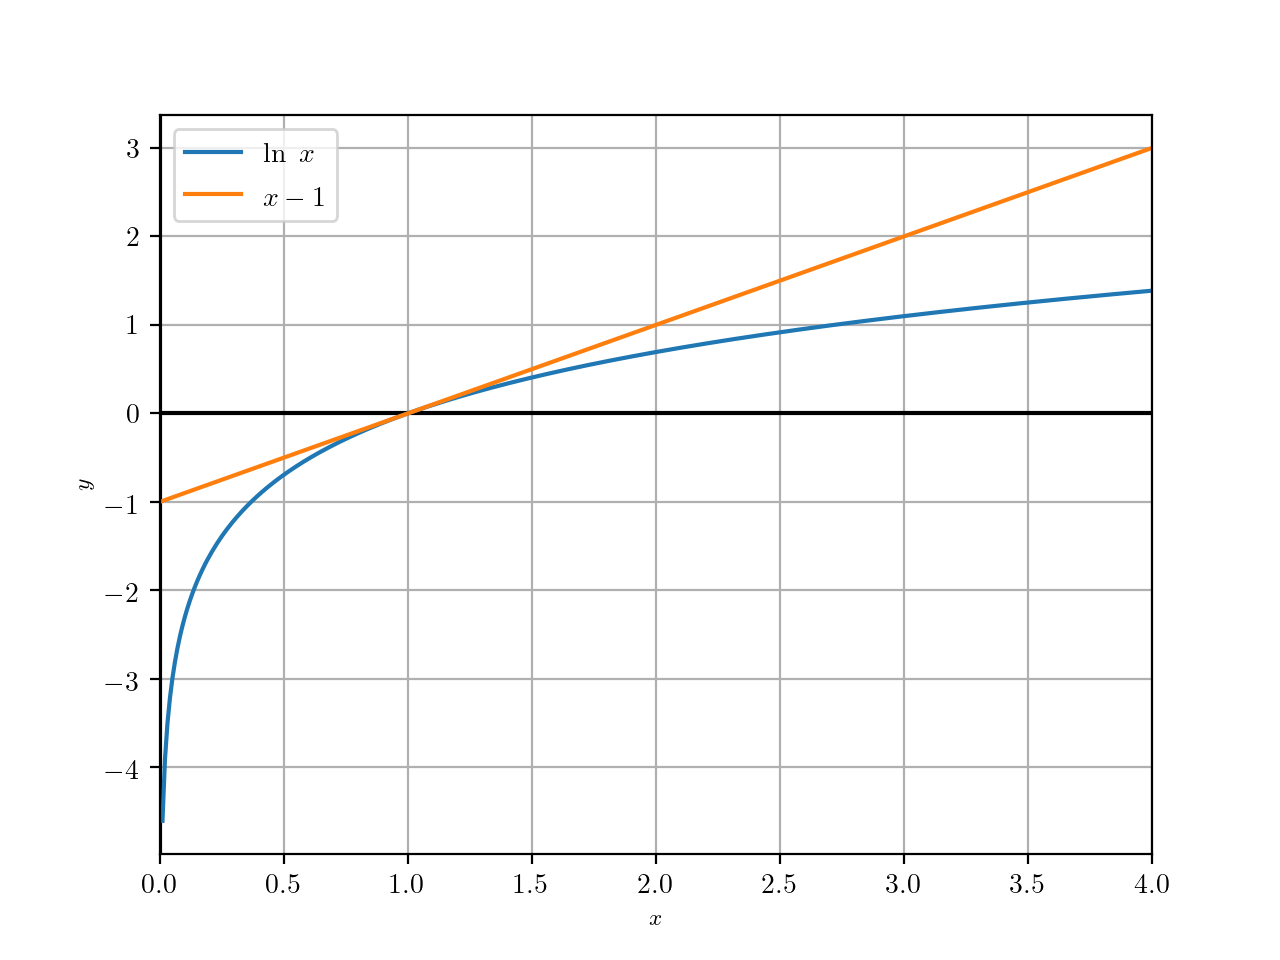
\includegraphics[scale=0.6]{lognep.png}
  \caption{Tracé du logarithme népérien}
  \label{fig:traceln}
\end{figure}
%
\begin{theo}
  L'ensemble \(E\) des fonctions dérivables de \(\R^{\Rplusetoile}\) telles que~:
  \begin{equation}
    \label{eq:fonclog}
    \forall x, y \in \Rplusetoile \quad f(xy)=f(x)+f(y)
  \end{equation}
  est la droite vectorielle engendrée par le logarithme népérien, c'est-à-dire que~:
  \begin{equation}
    E=\enstq{\fonction{f_{\alpha}}{\Rplusetoile}{\R}{x}{\alpha \ln x}}{\alpha \in \R}.
  \end{equation}
\end{theo}
\begin{proof}
  Soit une fonction \(f \in \R^{\Rplusetoile}\) dérivable sur \(\Rplusetoile\) vérifiant l'équation~\eqref{eq:fonclog}. Comme \(f\) est dérivable, on peut dériver l'équation~\eqref{eq:fonclog} par rapport à \(x\) et on obtient pour tout \(y\) strictement positif
  \begin{equation}
    y f'(xy)=f'(x).
  \end{equation}
  Pour \(x=1\), on a
  \begin{equation}
    y f'(y)=f'(1),
  \end{equation}
  c'est-à-dire \(f'(y)=f'(1) \ln' y\). Donc en intégrant cette équation à partir de \(1\), on a
  \begin{equation}
    f(y)=f'(1)\ln y + f(1).
  \end{equation}
  En appliquant l'équation~\eqref{eq:fonclog} en \(x=y=1\), on a \(f(1)=2f(1)\) donc \(f(1)=0\).

  On a montré que si une fonction \(f\) de \(\R^{\Rplusetoile}\) dérivable vérifie l'équation~\eqref{eq:fonclog}, alors elle est proportionnelle au logarithme népérien. La réciproque est due au théorème~\ref{theo:lognep1}.
\end{proof}
%
\subsection{Logarithmes de base a}
\label{subsec:chap1-loga}
\begin{defdef}
  Soit un réel \(a\) de \(\Rplusetoile\setminus\{1\}\). On définit la fonction logarithme de base  \(a\), notée \(\log_a\) par \(\fonction{\log_a}{\Rplusetoile}{\R}{x}{\dfrac{\ln x}{\ln a}}\).
\end{defdef}
%
\begin{prop}
  \begin{itemize}
  \item \(\log_a(1)=0\);
  \item pour tout \(a \in\Rplusetoile\setminus\{1\}\), la fonction \(\log_a\) est dérivable, donc continue, sur \(\Rplusetoile\) et pour tout réel \(x\) strictement positif
    \begin{equation}
      \log_a'(x)=\frac{1}{x \ln a}.
    \end{equation}
  \end{itemize}
\end{prop}
\begin{proof}
  Ce sont des conséquences immédiates de la définition et des propriétés du logarithme népérien.
\end{proof}
%
\begin{prop}
  Soient \(x\) et \(y\) deux réels strictement positifs, \(a\) et \(b\) deux bases de logarithme~\footnote{Une base de logarithme est un réel strictement positif différent de 1}, alors~:
  \begin{gather}
    \log_a xy=\log_a x + \log_a y; \\
    \log_b x=\log_ba \log_ax; \\
    \log_{1/a} x=-\log_a x.
  \end{gather}
\end{prop}
\begin{proof}
  \begin{itemize}
  \item \(\log_a xy= \frac{\ln xy}{\ln a}= \frac{\ln x}{\ln a} +\frac{\ln y}{\ln a}=\log_ax+\log_ay\);
  \item \(\log_b x = \frac{\ln x}{\ln b}=\frac{\ln x}{\ln a} \times \frac{\ln a}{\ln b}=\log_ax \log_ba\);
  \item soit en prenant \(b=\frac{1}{a} \in \Rplusetoile-\{1\}\) alors \(\log_{\frac{1}{a}}x=\log_ax \log_{\frac{1}{a}}(a)=\log_ax \frac{\ln a}{-\ln a}=-\log_ax\).
  \end{itemize}
\end{proof}
Le logarithme décimal en base \(10\) et le logarithme binaire en base \(2\).
\begin{figure}
  \centering
  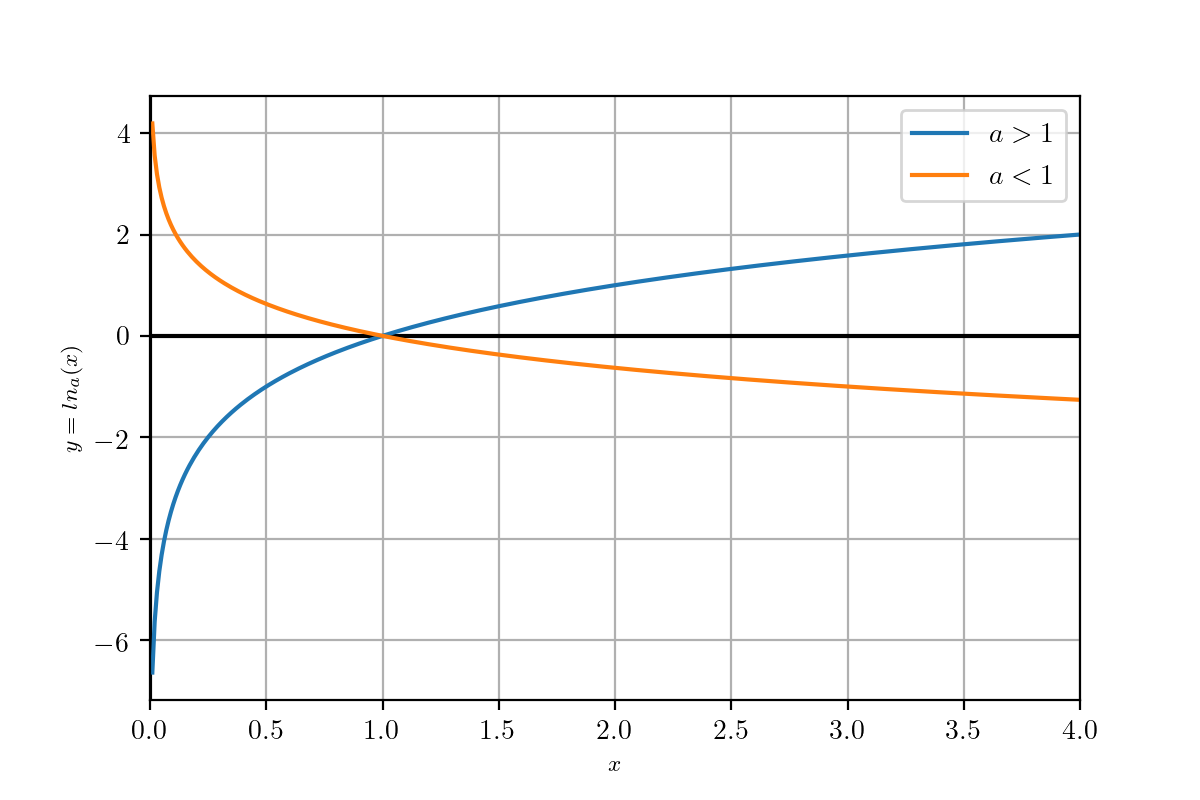
\includegraphics[scale=0.6]{logbase.png}
  \caption{Tracé des logarithmes de bases quelconque}
  \label{fig:traceloga}
\end{figure}
\subsection{Exponentielle}
\label{subsec:chap1-exp}
\begin{defdef}
  L'application logarithme népérien est continue sur \(\Rplusetoile\) et strictement croissante, telle que \(\lim\limits_{0^+} \ln =-\infty\) et \(\lim\limits_{+\infty} \ln = +\infty\). Alors le logarithme népérien induit une bijection de \(\Rplusetoile\) sur \(\R\). L'application réciproque du logarithme népérien est la fonction exponentielle notée \(\exp\) telle que
  \begin{equation}
    \fonction{\exp}{\R}{\Rplusetoile}{x}{\exp(x)}.
  \end{equation}
\end{defdef}
%
\begin{prop} Les fonctions logarithme népérien et exponentielle vérifient
  \begin{equation}
    \forall (x,y) \in \R \times \Rplusetoile \quad y=\exp(x) \iff x=\ln y.
  \end{equation}
\end{prop}
\begin{proof}
  C'est une conséquence de la définition.
\end{proof}
%
\begin{prop}
  La fonction exponentielle est dérivable sur \(\R\) et
  \begin{equation}
    \forall x \in \R \quad \exp'(x)=\exp(x).
  \end{equation}
\end{prop}
\begin{proof}
  La fonction \(\ln\) est dérivable sur \(\Rplusetoile\) et pour tout réel \(y\), \(\exp(y)>0\). Alors d'après les théorèmes généraux~\footnote{cf.\ annexe~\ref{chap:theogen}}, on a
  \begin{equation}
    \exp'(y)=\frac{1}{\ln'(\exp(y))}=\exp(y).
  \end{equation}
\end{proof}
%
\begin{prop} \label{prop-chap1:addexp}
  \begin{equation}
    \forall x, y \in \R \quad \exp(x+y)=\exp(x) \cdot \exp(y).
  \end{equation}
On dira plus tard que c'est un morphisme de groupes du  groupe additif \((\R,+)\) sur le groupe multiplicatif \((\R^*,\times)\)~\footnote{cf.\ chapitre~\ref{chap:groupes}}.

\end{prop}
\begin{proof}
  Soient deux réels \(x\) et \(y\). Comme
  \begin{equation}
    \ln(\exp(x+y))=x+y=\ln(\exp(x))+\ln(\exp(y))=\ln(\exp(x) \exp(y)),
  \end{equation}
  en appliquant l'exponentielle~\footnote{L'exponentielle est une fonction bijective} on obtient le résultat.
\end{proof}
%
\begin{prop}
  Soient \(x\) et \(y\) deux réels et un entier relatif \(n\), alors
  \begin{gather}
    \exp(-x)=\frac{1}{\exp(x)}; \\
    \exp(x-y)=\frac{\exp(x)}{\exp(y)}; \\
    \exp(nx)=\exp(x)^n.
  \end{gather}
\end{prop}
\begin{proof}
  \begin{itemize}
  \item \(\ln(\exp(-x))=-x=-\ln(\exp(x))=\ln \left(\frac{1}{\exp(x)}\right)\) et on peut composer par \(\exp\)~\footnote{Idem} pour obtenir le résultat;
  \item \(\exp(x-y)=\exp(x) \exp(-y)=\frac{\exp(x)}{\exp(y)}\);
  \item \(\ln(\exp(nx))=nx=n \ln(\exp(x))=\ln(\exp(x)^n)\) puis en composant par l'exponentielle, on a le résultat.
  \end{itemize}
\end{proof}
%
\begin{prop}
  La fonction exponentielle admet les limites suivantes~:
  \begin{gather}
    \lim\limits_{x \to \infty} \exp(x)=+\infty;\\
    \lim\limits_{x \to -\infty} \exp(x)=0;\\
    \lim\limits_{x \to 0} \frac{\exp(x)-1}{x}=1.
  \end{gather}
\end{prop}
\begin{proof}
  Les deux premières propositions sont des conséquences de la définition et la dernière est la limite du taux d'accroissement en zéro, soit la dérivée en 0 de l'exponentielle.
\end{proof}
%
\begin{figure}
  \centering
  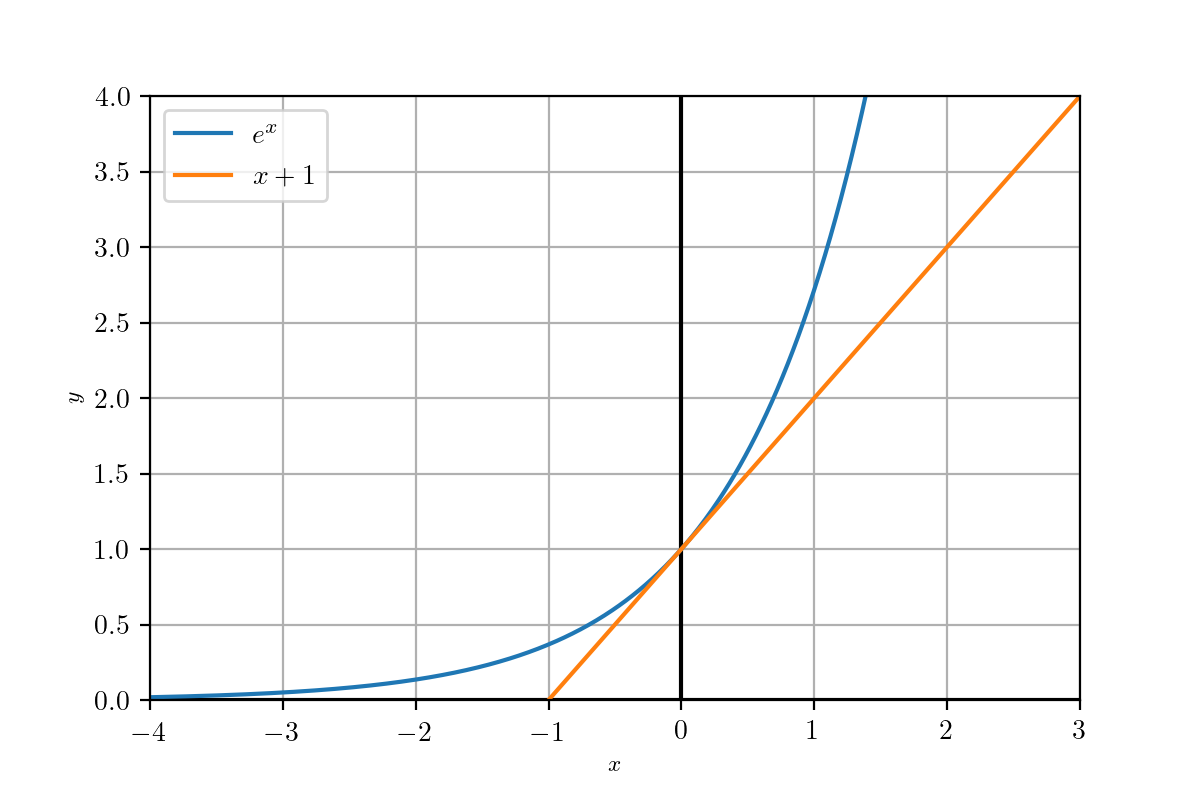
\includegraphics[scale=0.6]{exp.png}
  \caption{Tracé de l'exponentielle}
  \label{fig:traceexp}
\end{figure}
%
\begin{theo}
  L'ensemble \(E\) des fonctions de \(\R^{\R}\) dérivables qui vérifient l'équation
  \begin{equation}
    \label{eq:foncexp}
    \forall x, y \in \R \quad f(x+y)=f(x) \cdot f(y)
  \end{equation}
  est
  \begin{equation}
    E=\left\{0\right\} \cup \enstq{\fonction{g_{\alpha}}{\R}{\R}{x}{\exp(\alpha x)}}{\alpha \in \R}.
  \end{equation}
\end{theo}
\begin{proof}
  Soit une fonction \(f \in \R^{\R}\) dérivable qui vérifie l'équation~\eqref{eq:foncexp}, alors en dérivant cette équation on obtient~:
  \begin{equation}
    \label{eq:foncexpun}
    f'(x+y)=f'(x)f(y)=f(x)f'(y).
  \end{equation}
  Deux cas sont possibles~:
  \begin{itemize}
  \item la fonction nulle est solution,
  \item si la fonction n'est pas nulle, il existe une réel \(x_0\) tel que \(f(x_0) \neq 0\). Alors
    \begin{equation}
      \forall y \in \R \quad f(x_0)= f(x_0-y)f(y).
    \end{equation}
    Soit \(y \in \R\), alors \(f(y) \neq 0\). La fonction \(f\) ne s'annulant donc jamais, on peut reprendre l'équation~\ref{eq:foncexpun} et écrire que
    \begin{equation}
      \label{eq:foncexpdeux}
      \forall x \in \R \quad \frac{f'(x)}{f(x)}=\frac{f'(0)}{f(0)}.
    \end{equation}
    D'après l'équation~\ref{eq:foncexp}, on a
    \begin{equation}
      f(0)=f(0)^2.
    \end{equation}
    Comme \(f\) ne s'annule pas, nécessairement \(f(0)=1\). La fonction \(f\) est donc toujours positive. D'après l'équation~\eqref{eq:foncexpdeux}, il existe un réel \(c\) tel que
    \begin{equation}
      \forall x \in \R \quad \ln \abs{f(x)}=\ln f(x)=f'(0) x + c.
    \end{equation}
    Alors
    \begin{equation}
      f(x)=\exp(f'(0) x +c),
    \end{equation}
    et comme \(f(0)=1\), on a \(c=0\).
  \end{itemize}
  La réciproque est due à la proposition~\ref{prop-chap1:addexp}. Si une fonction est dans \(E\) alors elle vérifie l'équation~\ref{eq:foncexp}.
\end{proof}
%
\subsection{Exponentielles de base a}
\label{subsec:chap1-expa}
\begin{defdef}
  Soit une base \(a\) de logarithme dans \(\Rplusetoile\setminus\{1\}\). Comme l'application logarithme népérien, l'application \(\log_a\) induit une bijection de \(\Rplusetoile\) sur \(\R\) et admet une bijection réciproque appelée exponentielle de base \(a\), notée \(\exp_a\).
\end{defdef}
\begin{prop}
  \begin{equation}
    \forall x \in \R \ \forall y \in \Rplusetoile \ \forall a \in \Rplusetoile\setminus\{1\} \quad y=\exp_a(x) \iff x=\log_a(y).
  \end{equation}
\end{prop}
\begin{proof}
  C'est une conséquence directe de la définition.
\end{proof}
%
\begin{prop}
  \begin{equation}
    \forall x \in \R \ \forall a \in \Rplusetoile\setminus\{1\} \quad \exp_a(x)=\exp(a\ln x).
  \end{equation}
\end{prop}
\begin{proof}
  On sait que~:
  \begin{equation}
    \log_a(\exp_a(x))=x=\frac{\ln(\exp(x \ln a))}{\ln a}=\log_a(\exp(x \ln a)),
  \end{equation}
  et en appliquant \(\exp_a\), qui est bijective, on obtient le résultat.
\end{proof}
%
\begin{prop}
  Soient \(a\) une base de logarithme, \(x\) et \(y\) deux réels et \(n\) un entier relatif. Alors les propriétés suivantes sont vraies~: la fonction \(\exp_a\) est indéfiniment dérivable sur \(\R\) et
  \begin{equation}
    \forall x \in \R \quad \exp_a'(x)=\ln a \exp_a(x).
  \end{equation}
 De plus~:
  \begin{gather}
    \exp_a(x+y)=\exp_a(x) \exp_a(y); \\
    \exp_a(-x)=\frac{1}{\exp_a(x)}; \\
    \exp_a(x-y)=\frac{\exp_a(x)}{\exp_a(y)}; \\
    \exp_a(nx)=\exp_a(x)^n;\\
    \exp_{\frac{1}{a}}(x)=\exp(-x \ln a)=\exp_a(-x).
  \end{gather}
\end{prop}
\begin{proof}
  Ce sont des conséquences immédiates des propriétés de l'exponentielle.
\end{proof}
%
En appliquant la formule précédente en \(x=1\), et on a~: \(\exp_a(n)=\exp_a(1)^n=a^n\). Alors on pose
\begin{equation}
  \forall x \in \R \quad a^x=\exp_a(x)=\exp(x \ln a)
\end{equation}
En particulier pour l'exponentielle~: \(\e^x=\exp(x)\). On pose aussi que pour tout réel \(x\), \(1^x=1\). Donc \(\forall a>0 \ \forall x>0 \quad a^x=\exp(x \ln a)\).
%
\begin{figure}
  \centering
  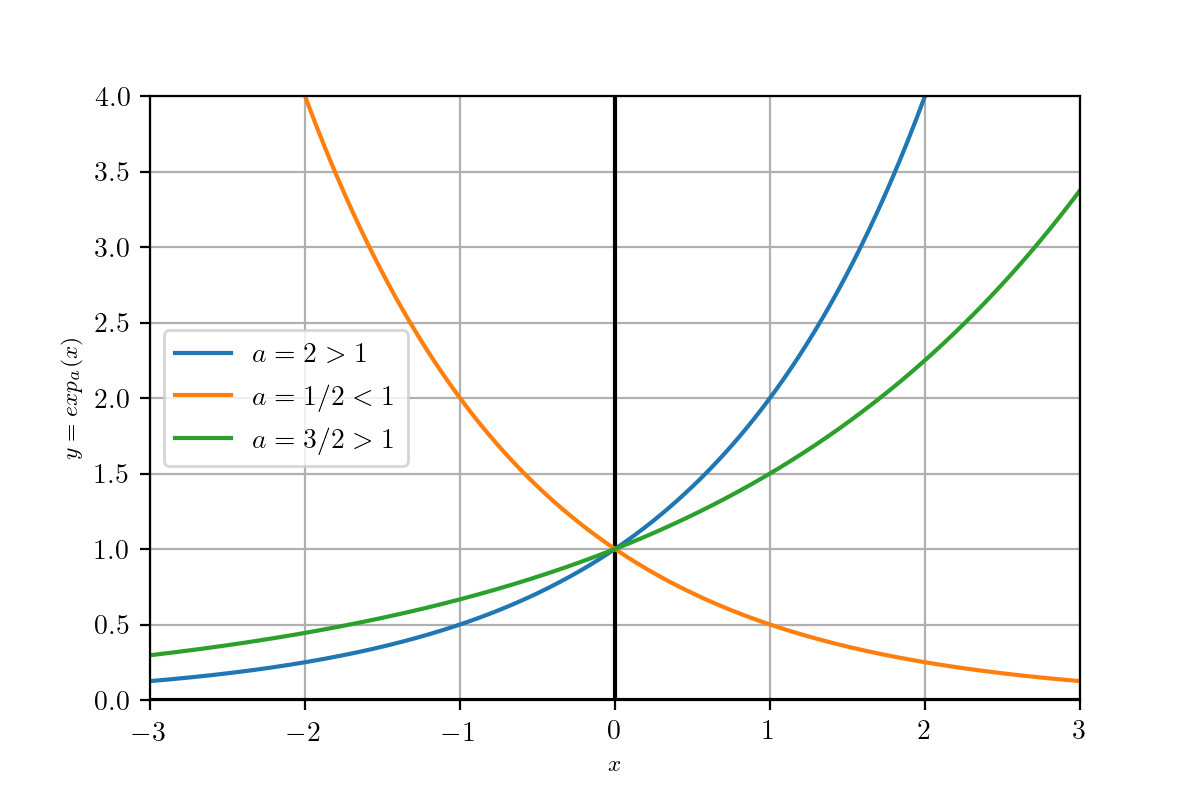
\includegraphics[scale=0.6]{expa.png}
  \caption{Tracé des exponentielles de base quelconque}
  \label{fig:traceexpa}
\end{figure}
%
\section{Puissances}
\label{sec:chap1-puissances}
\subsection{Les fonctions puissances}
\label{subsec:chap1-fonctionspuissances}
\begin{defdef}
  Soit un réel \(\alpha\). On appelle fonction puissance d'exposant \(\alpha\) la fonction
  \begin{equation}
    \fonction{f_{\alpha}}{\Rplusetoile}{\R}{x}{x^{\alpha}=\e^{\alpha \ln x}}.
  \end{equation}
\end{defdef}
%
\begin{prop}
  Soient deux réels \(\alpha\) et \(x\), alors les formules suivantes sont vraies~:
  \begin{gather}
    1^{\alpha}=1; \\
    x^0=1; \\
    \ln x^{\alpha} = \alpha \ln x.
  \end{gather}
\end{prop}
\begin{proof}
  Ce sont des conséquences immédiates de la définition.
\end{proof}
%
\begin{prop}
  Soient deux réels \(\alpha\) et \(\beta\), puis deux réels strictement positifs \(x\) et \(y\). Les formules suivantes sont vraies
  \begin{gather}
    x^{\alpha+\beta}=x^\alpha x^\beta;\\
    (xy)^\alpha = x^\alpha y^\alpha;\\
    (x^\alpha)^\beta=x^{\alpha\beta}.
  \end{gather}
\end{prop}
\begin{proof}
  Soient deux réels \(\alpha\) et \(\beta\), puis deux réels strictement positifs \(x\) et \(y\). Alors
  \begin{gather}
  x^{\alpha+\beta}=\e^{(\alpha+\beta)\ln x}=\e^{\alpha \ln x} \e^{\beta \ln x}=x^\alpha x^\beta;\\
  (xy)^\alpha=\e^{\alpha \ln (xy)}=\e^{\alpha \ln x +\alpha \ln y}=\e^{\alpha \ln x} \e^{\alpha \ln y}=x^\alpha x^\beta ;\\
  (x^\alpha)^\beta=(\e^{\alpha \ln x})^\beta=\e^{\beta \ln(\e^{\alpha \ln x})}=\e^{\beta \alpha \ln x}=x^{\alpha \beta}.
  \end{gather}
\end{proof}

Les fonctions puissances admettent les limites suivantes~:
\begin{equation}
  \begin{cases}
    \alpha=0 & f_0=\tilde{1};\\
    \alpha>0 & \lim\limits_{+\infty}f_\alpha=+\infty \quad \lim\limits_{0^{+}}f_\alpha=0;\\
    \alpha<0 & \lim\limits_{+\infty}f_\alpha=0 \quad \lim\limits_{0^{+}}f_\alpha=+\infty.
  \end{cases}
\end{equation}
\begin{prop}
  Pour tout \(\alpha \in \R\), la fonction \(f_\alpha\) est dérivable sur \(\Rplusetoile\) telle que
  \begin{equation}
    \forall x \in \Rplusetoile \quad f'_\alpha(x)=\alpha x^{\alpha -1}.
  \end{equation}
\end{prop}
\begin{proof}
  La fonction \(f_\alpha\) est dérivable par composition de fonctions qui le sont et pour tout \(x > 0\) on a
  \begin{equation}
    f_\alpha'(x)=\frac{\alpha}{x} \e^{\alpha \ln x}=\frac{\alpha}{x} x^\alpha=\alpha x^{\alpha-1}.
  \end{equation}
\end{proof}

Lorsque \(\alpha \geqslant 0\), les fonctions \(f_\alpha\) peuvent se prolonger en zéro pour obtenir une fonction continue. Deux cas se présentent~:
\begin{itemize}
\item Si \(\alpha>0\) on pose \(\fonction{\tilde{f}_\alpha}{\Rpluss}{\R}{x}{\begin{cases} f_\alpha(x) & x>0 \\ 0 & x=0 \end{cases}}\);
\item Si \(\alpha=0\) on pose \(\fonction{\tilde{f}_0}{\Rpluss}{\R}{x}{1}\).
\end{itemize}
Le prolongement en zéro des fonction puissances s'effectue de cette manière~:
\begin{itemize}
\item Si \(\alpha=0 \quad \tilde{f}_0\) est dérivable et sa dérivée est nulle;
\item Si \(\alpha>1 \quad x^{\alpha-1}\underset{x \to 0^+}{\longrightarrow}0\), le prolongement par continuité \(\tilde{f}_\alpha\) est dérivable en 0 et \(\tilde{f}_\alpha'(0)=0\) La courbe admet une tangente horizontale;
\item Si \(\alpha=1 \quad x^{\alpha-1}\underset{x \to 0^+}{\longrightarrow}1\), le prolongement  \(\tilde{f}_1\) est dérivable en 0 et \(\tilde{f}_1'(0)=1\);
\item Si \(0<\alpha<1 \quad x^{\alpha-1}\underset{x \to 0^+}{\longrightarrow}+\infty \), le prolongement \(\tilde{f}_\alpha\) n'est pas dérivable en zéro et la courbe admet une tangente verticale.
\end{itemize}
%
\begin{figure}
  \centering
  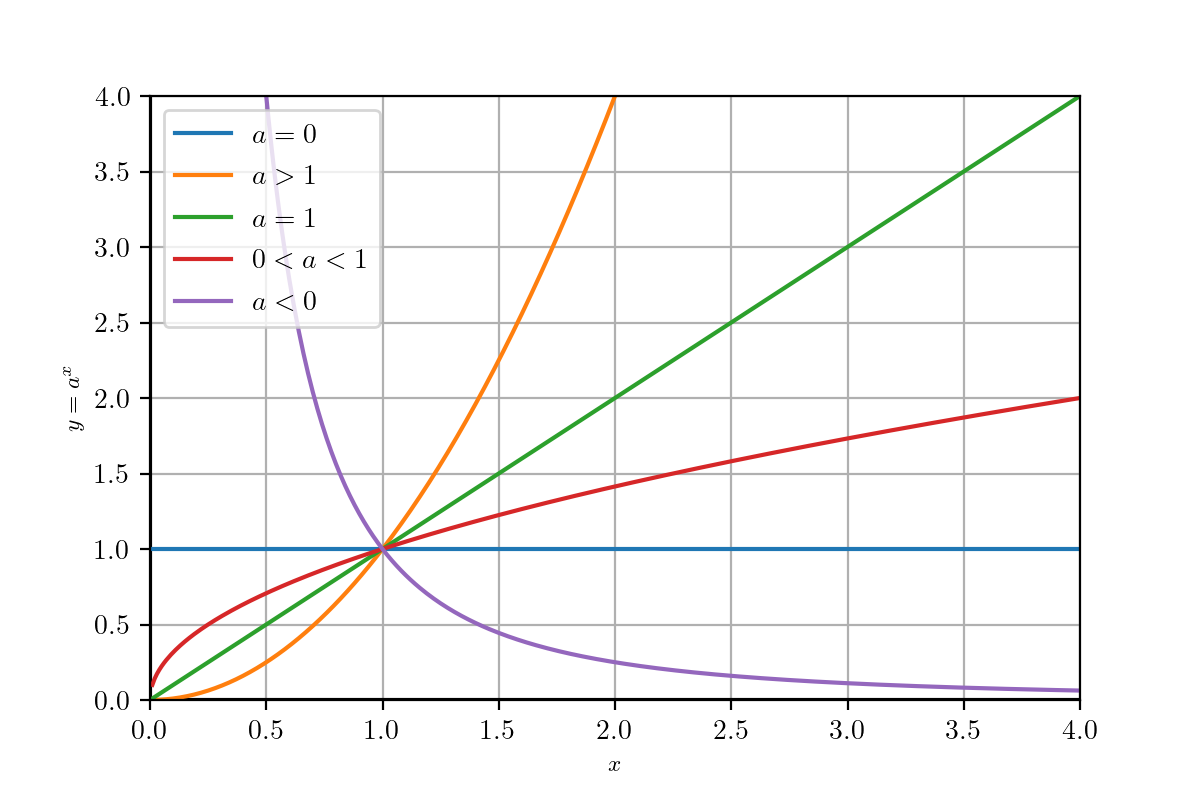
\includegraphics[scale=0.6]{puiss.png}
  \caption{Tracé de quelques fonctions puissance}
  \label{figtracepuissance}
\end{figure}

Si \(\alpha \neq 0\), les fonctions \(f_{\frac{1}{\alpha}}\) et \(f_\alpha\) sont réciproques l'une de l'autre.
%
\subsection{Dérivation des fonctions de la forme exponentielle}
\label{subsec:chap1-derivationdesfonctionsdelaformeexponentielle}
\begin{prop}
  Soient \(I\) un intervalle réel, \(u\) et \(v\) des fonctions dérivables de \(\R^{I}\), alors la fonction \(u^v\) est dérivable.
\end{prop}
\begin{proof}
  Soit un réel \(x\) de \(I\) et soit \(f(x)=\e^{v(x) \ln u(x)}\). La fonction \(f\) est dérivable comme produit et composée de fonctions qui le sont, et
  \begin{align}
    f'(x) &=\left[ v'(x) \ln u(x) + v(x) \frac{u'(x)}{u(x)} \right]\e^{v(x) \ln u(x)} \\
    &= \left[v'(x)u(x)\ln u(x) + v(x) u'(x) \right]u(x)^{v(x)-1}.
  \end{align}
\end{proof}
%
\section{Croissances comparées}
\label{sec:chap1-croissancescomparees}
\begin{theo}
  \begin{equation}
    \lim\limits_{x \to +\infty} \frac{\ln x}{x}=0^+.
  \end{equation}
  Ce qui traduit la \og lenteur \fg{} de croissance du logarithme népérien par rapport à l'identité. On écrira par la suite \(\ln x=o_{+\infty}(x)\).
\end{theo}
\begin{proof}
  Soient deux réels \(x\) et \(t\) supérieurs à 1, alors
  \begin{align}
    \sqrt{t} & \leqslant t \\
    \frac{1}{t} &\leqslant \frac{1}{\sqrt{t}}\\
    0 \leqslant \ln x = \int_{1}^{x} \frac{\diff t}{t} &\leqslant \int_1^x\frac{\diff t}{\sqrt{t}}=2\sqrt{x}-2\\
    0 \leqslant \frac{\ln x}{x} &\leqslant \frac{2}{\sqrt{x}} - \frac{2}{x}.
  \end{align}
  En passant à la limite, et d'après le théorème des gendarmes on obtient la limite en zéro.
\end{proof}
%
\begin{prop}
  \label{prop-chap1:croissancecomparelnpuissance}
  Soient \(\alpha\) et \(\beta\) deux réels strictement positifs, alors
  \begin{equation}
    \lim\limits_{x \to +\infty} \frac{(\ln x)^\alpha}{x^\beta} = 0^+ \quad \lim\limits_{x \to 0^+} x^\beta \abs{\ln x}^\alpha=0^+.
  \end{equation}
  Ce qui veut dire que les puissances \og l'emportent \fg{} toujours devant les logarithmes.
\end{prop}
\begin{proof}
  Soit un réel \(x \geqslant 1\) alors
  \begin{equation}
    \frac{\ln x^\alpha}{x^\beta}=\left(\frac{\alpha}{\beta} \frac{\ln x^{\frac{\beta}{\alpha}}}{x^{\frac{\beta}{\alpha}}} \right)^\alpha.
  \end{equation}
  On a
  \begin{equation}
    x^{\frac{\beta}{\alpha}}\underset{x \to +\infty}{\longrightarrow}+\infty,
  \end{equation}
  donc par composition de limites
  \begin{equation}
    \lim\limits_{x \to \infty} \frac{\ln x^{\frac{\beta}{\alpha}}}{x^{\frac{\beta}{\alpha}}}=0^{+}.
  \end{equation}
  Ainsi
  \begin{equation}
    \frac{\ln x ^\alpha}{x^\beta}=\e^{\alpha \ln \left(\frac{\alpha}{\beta} \frac{\ln x^{\frac{\beta}{\alpha}}}{x^{\frac{\beta}{\alpha}}} \right)} \underset{x \to +\infty}{\longrightarrow}0.
  \end{equation}
  La deuxième limite peut s'obtenir en faisant apparaître \(\frac{1}{x}\)~: soit un réel \(x\) tel que \(0<x<1\), alors
  \begin{equation}
    x^\beta \abs{\ln x}^\alpha=\frac{\abs{-\ln\left(\frac{1}{x}\right)}^\alpha}{\left(\frac{1}{x} \right)^\beta}=\frac{\ln\left(\frac{1}{x}\right)^\alpha}{\left(\frac{1}{x}\right)^\beta}.
  \end{equation}
  Soit en appliquant la première limite ---~puisque \(\frac{1}{x}\underset{x \to 0^+}{\longrightarrow}+\infty\)~--- on obtient le résultat.
\end{proof}
%
\begin{prop}
  Soient \(\alpha\) et \(\beta\) deux réels strictement positifs, alors
  \begin{equation}
    \lim\limits_{x \to + \infty} \frac{\e^{\alpha x}}{x^\beta}=+\infty \quad \lim\limits_{x \to -\infty} \e^{\alpha x} \abs{x}^\beta=0^+.
  \end{equation}
  Ce qui traduit la prépondérance des fonctions exponentielles face aux fonctions puissances.
\end{prop}
%
\begin{proof}
  Soit un réel \(x\) strictement positif. On pose \(y=\e^{x}\) alors
  \begin{equation}
    \frac{\e^{\alpha x}}{x^\beta}=\frac{y^\alpha}{\ln(y)^\beta},
  \end{equation}
  puisque \(\e^{x} \underset{x \to \infty}{\longrightarrow}+\infty\) la proposition~\ref{prop-chap1:croissancecomparelnpuissance} nous permet d'écrire que par composition de limites, la première limite est vraie
  \begin{equation}
    \lim\limits_{x \to + \infty} \frac{\e^{\alpha x}}{x^\beta}=+\infty.
  \end{equation}
  Soit un réel \(x\) strictement négatif, alors
  \begin{equation}
    \e^{\alpha x}\abs{x}^\beta=\frac{(-x)^\beta}{\e^{\alpha(-x)}}.
  \end{equation}
  D'après la première limite
  \begin{equation}
    \lim\limits_{x \to - \infty} \frac{\e^{\alpha (-x)}}{(-x)^\beta}=+\infty.
  \end{equation}
  D'où
  \begin{equation}
    \lim\limits_{x\to -\infty}\frac{(-x)^\beta}{\e^{\alpha (-x)}}=\lim\limits_{x \to -\infty} \e^{\alpha x} \abs{x}^\beta=0^+.
  \end{equation}
\end{proof}
%
\section{Trigonométrie circulaire}
\label{sec:chap1-trigocirc}
On présente un tableau récapitulatif~\ref{tab:fonctiontrigo} des différentes fonctions trigonométriques de base et leurs propriétés. On a tracé les mêmes fonctions sur le cercle trigonométrique de la figure~\ref{fig:cercletrigo}.
\begin{table}[!h]
  \centering
  \begin{tabular}{|c|c|c|c|c|}
    \hline
    Nom & définie sur & parité & T & propriétés \\ \hline
    sinus & \(\R\) & impaire & \(2\pi\) & \(\sin(\pi+x)=-\sin x\) \\
    & & & & \(\sin(\pi-x)=\sin x\) \\ \hline
    cosinus & \(\R\) & paire & \(2\pi\) & \(\cos(\pi+x)=-\cos x\)\\
    & & & & \( \sin(\pi-x)=-\cos x\) \\ \hline
    tangente & \(D_1=\R\setminus\{\frac{\pi}{2}+\pi \Z\}\) & impaire & \(\pi\) & \(\tan x =\frac{\sin x}{\cos x}\) \\ \hline
    cotangente & \(D_2=\R\setminus\{\pi \Z\}\) & paire & \(\pi\) & \(\cot x =\frac{\cos x}{\sin x}\) \\ \hline
  \end{tabular}
  \caption{Fonctions trigonométriques de base}
  \label{tab:fonctiontrigo}
\end{table}

%\begin{figure}
%\centering
%\begin{tikzpicture}
%\draw (0,0) circle (4);
%\draw (180:4) -- (0:4);
%\draw (-90:4) -- (90:4);
%\draw (1,0) arc(0:35:1) node[right, below]{\(\theta\)};
%\draw (0,0) -- (35:4) node[midway, above, sloped]{\(1\)};
%\draw[color=blue] (35:4) -- (0,2.29) node[midway, above, sloped]{\(\cos \theta\)};
%\draw[color=red] (35:4) -- (3.276,0) node[midway, below, sloped]{\(\sin \theta\)};
%%\draw (4,-4) --++ (0,8);
%\draw[color=yellow](35:4) -- (4,2.8);%Pour compléter la tangente
%\draw[color=orange](4,2.8) -- (5.71,4);
%\draw[color=green] (4,0) -- (4,2.8) node[midway, below, sloped]{\(\tan \theta\)};
%\draw[color=pink] (0,4) -- (5.71,4) node[midway, above, sloped]{\(\cot \theta\)};
%\end{tikzpicture}
%\caption{Cercle trigonométrique}
%\label{fig:cercletrigo}
%\end{figure}
\begin{figure}
\centering
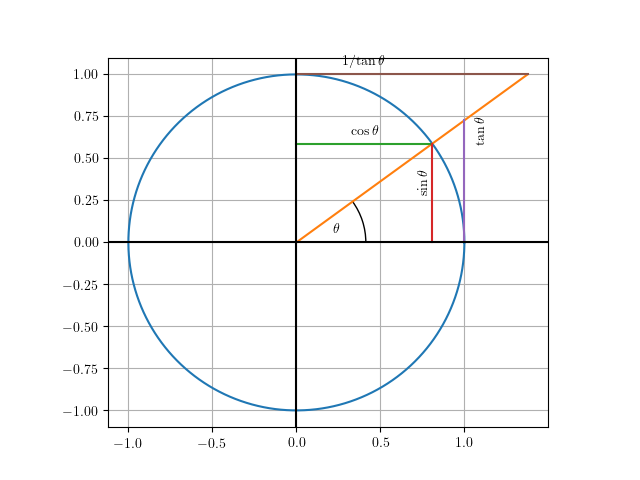
\includegraphics[scale=0.7]{./CercleTrigo.png}
\caption{Cercle trigonométrique}
\label{fig:cercletrigo}
\end{figure}
%
Soit un réel \(x\) et un réel \(y \in D_2\), alors
\begin{gather}
  \cos^2 x+\sin^2 x=1;\\
  \sin \left(\frac{\pi}{2}-x\right)=\cos x=\sin \left(\frac{\pi}{2}+x\right); \\
  \cos \left(\frac{\pi}{2}-x\right)=\sin x=-\cos\left(\frac{\pi}{2}+x\right);\\
  \tan \left(\frac{\pi}{2}-y \right)=\cot y=-\cot \left(\frac{\pi}{2}+y\right).
\end{gather}
%
\begin{figure}
  \centering
  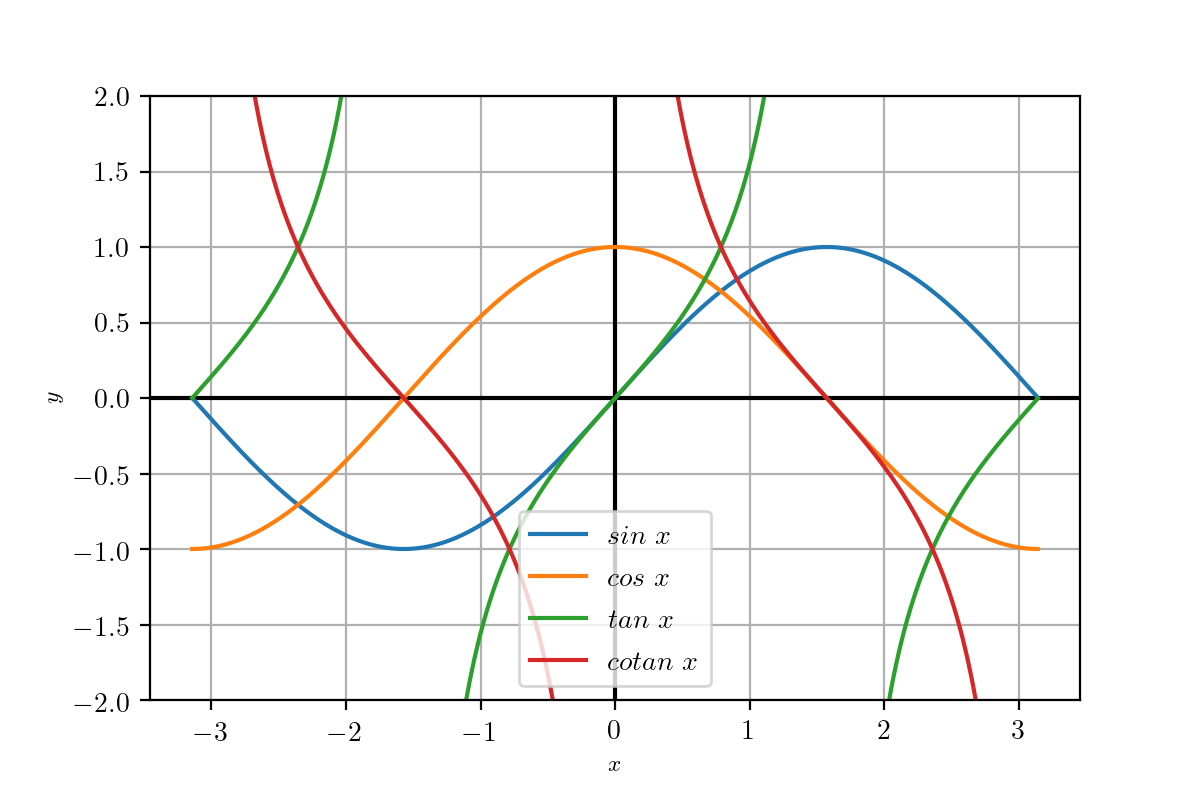
\includegraphics[scale=0.6]{trig.png}
  \caption[Tracé de quelques fonctions trigonométriques]{Tracé de quelques fonctions trigonométriques. En rouge sinus, en bleu cosinus, en vert tangente et en rose cotangente}
  \label{fig:tracetrigo}
\end{figure}
%
\renewcommand{\arraystretch}{2.2}
\begin{table}
  \centering
  \begin{tabular}{|c|c|c|c|c|c|}
    \hline
    \(\displaystyle x\)& \(\displaystyle 0\)&\(\displaystyle \frac{\pi}{6}\)&\(\displaystyle \frac{\pi}{4}\)&\(\displaystyle \frac{\pi}{3}\)&\(\displaystyle \frac{\pi}{2}\)\\ \hline
    \(\displaystyle \sin x\) &\(\displaystyle  0\) &\(\displaystyle  \frac{1}{2}\) &\(\displaystyle  \frac{\sqrt{2}}{2}\) & \(\displaystyle \frac{\sqrt{3}}{2}\) &\(\displaystyle  1 \)\\ \hline
    \(\displaystyle \cos x\) &\(\displaystyle  1 \)&\(\displaystyle \frac{\sqrt{3}}{2}\) & \(\displaystyle \frac{\sqrt{2}}{2}\) & \(\displaystyle \frac{1}{2}\) & \(\displaystyle 0\) \\ \hline
    \(\displaystyle \tan x\) & \(\displaystyle  0 \)&\(\displaystyle \frac{1}{\sqrt{3}}\) & \(\displaystyle 1\) & \(\displaystyle \sqrt{3}\) & \(\displaystyle \infty\) \\ \hline
    \(\displaystyle \cot x\) & \(\displaystyle \infty\) & \(\displaystyle \sqrt{3}\) &\(\displaystyle  1\) & \(\displaystyle \frac{1}{\sqrt{3}}\) &\(\displaystyle  0\)\\ \hline
  \end{tabular}
  \caption{Valeurs particulières des fonctions trigonométriques}
  \label{tab:valeurpart}
\end{table}
\renewcommand{\arraystretch}{1}
\paragraph{Dérivées}
Les fonctions sinus, cosinus, tangente et cotangente sont dérivables sur leurs ensembles de définition, et on a:
\begin{gather}
\forall x \in \R \quad \sin'x=\cos x \ \cos'x=-\sin x; \\
\forall x \in D_1 \quad \tan'x=\frac{1}{\cos^2 x}=1+\tan^2 x; \\
\forall x \in D_2 \quad \cot'x=\frac{-1}{\sin^2 x}=-1-\cot^2 x.
\end{gather}
\begin{prop}
  Les fonctions trigonométriques vérifient les égalités suivantes~:
  \begin{gather}
    \forall x, y \in \R \quad \cos x = \cos y \iff \exists k \in \Z \ x=\pm y + 2k\pi;\\
    \forall x, y \in \R \quad \sin x = \sin y \iff \begin{cases} \exists k \in \Z & x = y + 2 k \pi \\ \exists k \in \Z & x = \pi - y + 2 k \pi\end{cases}; \\
    \forall x, y \in D_1 \quad \tan x = \tan y \iff \exists k \in \Z \ x = y + k \pi;\\
    \forall x, y \in D_2 \quad \cot x = \cot y \iff \exists k \in \Z \ x = y + k \pi.
  \end{gather}
\end{prop}

\section{Fonctions circulaires réciproque}
\label{sec:chap1-fonctionscircréciproques}
\subsection{Fonction arcsinus}
\label{subsec:chap1-fonctionarcsinus}
\begin{defdef}
  La fonction \(\fonction{\sin}{\intervalleff{-\frac{\pi}{2}}{\frac{\pi}{2}}}{\intervalleff{-1}{1}}{x}{\sin x}\) est une bijection~\footnote{parce qu'elle est continue, strictement croissante telle que \(\sin -\frac{\pi}{2}=-1\)  et \(\sin \frac{\pi}{2}=1\)} et cette bijection admet une réciproque appelée arcsinus notée \(\arcsin\).
\end{defdef}
%
\begin{prop}
  \begin{equation}
    \forall x \in \intervalleff{-\frac{\pi}{2}}{\frac{\pi}{2}} \forall y \in \intervalleff{-1}{1} \quad y = \sin x \iff x = \arcsin y;
  \end{equation}
  et
  \begin{gather}
    \sin(\arcsin y)) = y, \\
    \arcsin(\sin x) = x.
  \end{gather}
\end{prop}
\begin{proof}
  C'est une conséquence de la définition de \(\arcsin\).
\end{proof}
\emph{Remarque~:} La formule \(\arcsin(\sin x) = x\) n'est valable que dans \(\intervalleff{-\frac{\pi}{2}}{\frac{\pi}{2}}\) et la deuxième dans \(\intervalleff{-1}{1}\).
%
\begin{prop}
  La fonction \(\arcsin\) est impaire et strictement croissante.
\end{prop}
\begin{proof}
  La fonction \(\arcsin\) est croissante par construction car sa réciproque est strictement croissante. Ensuite, l'intervalle \(\intervalleff{-1}{1}\) est centré en 0 et puisque sinus est impaire on a
  \begin{equation}
    \forall y \in \intervalleff{-1}{1} \quad \sin (\arcsin -y)=-y=-\sin(\arcsin y)=\sin (-\arcsin y).
  \end{equation}
  En appliquant la fonction \(\arcsin\)~\footnote{qui est bijective} à chaque membre, on trouve que la fonction \(\arcsin\) est impaire.
\end{proof}
%
\begin{prop}
  La fonction arcsinus est dérivable sur \(\intervalleoo{-1}{1}\) et
  \begin{equation}
    \forall y \in \intervalleoo{-1}{1} \quad \arcsin'y = \frac{1}{\sqrt{1-y^2}}.
  \end{equation}
\end{prop}
\begin{proof}
  La fonction sinus est dérivable sur \(\intervalleff{-\frac{\pi}{2}}{\frac{\pi}{2}}\) telle que \(\sin'=\cos\). Si \(y=\pm 1\) alors \(\cos(\arcsin y)=0\) et donc arcsinus n'est pas dérivable. De plus la courbe représentative admet des tangentes verticales en \(-1\) et \(1\). Si \(y \in \intervalleoo{-1}{1}\), alors \(\cos(\arcsin y) \neq 0\), arcsinus et donc dérivable en \(y\) et
  \begin{equation}
    \arcsin' y = \frac{1}{\cos( \arcsin y)}=\frac{1}{\sqrt{1-\sin^2(\arcsin y)}}=\frac{1}{\sqrt{1-y^2}}.
  \end{equation}
\end{proof}
\begin{figure}
  \centering
  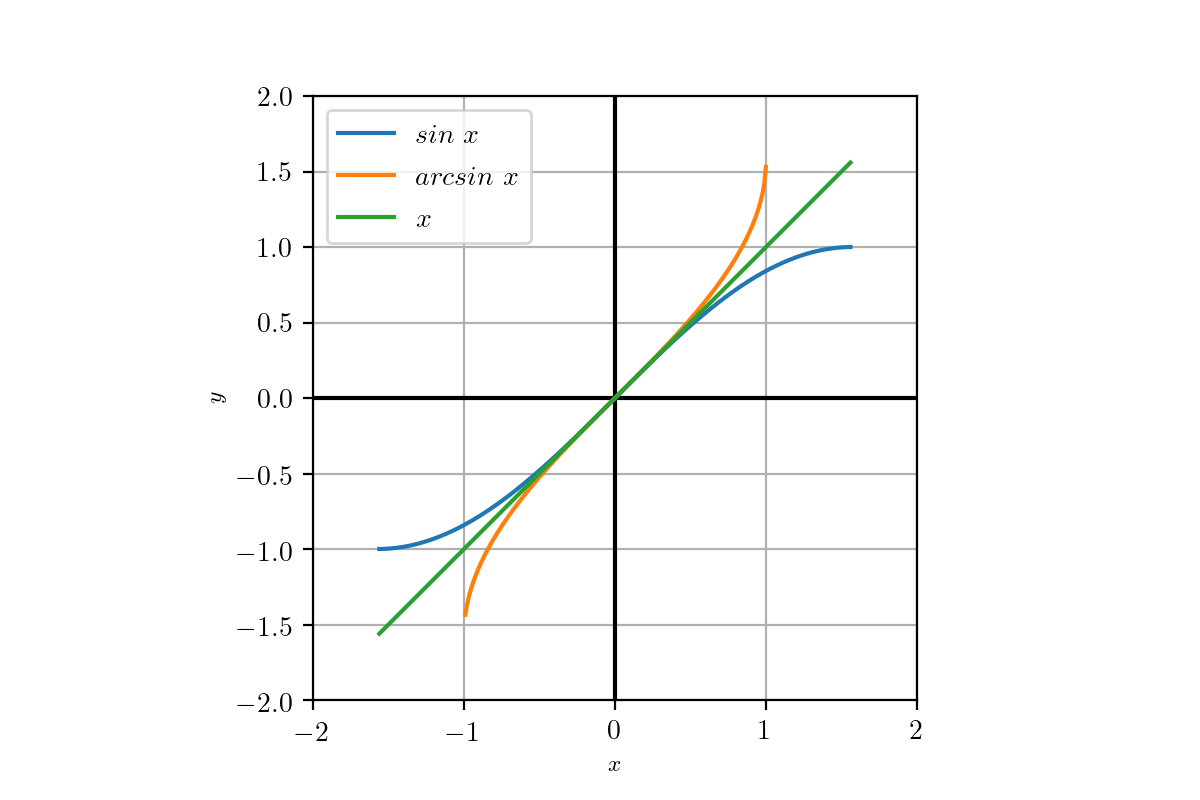
\includegraphics[scale=0.7]{arcsin.png}
  \caption{Tracé de arcsinus}
  \label{fig:tracearcsinus}
\end{figure}
%
\subsection{Fonction arccosinus}
\label{subsec:chap1-fonctionarccos}
\begin{defdef}
  La fonction \(\fonction{\cos}{\intervalleff{0}{\pi}}{\intervalleff{-1}{1}}{x}{\cos x}\) est une bijection~\footnote{parce qu'elle est continue, strictement décroissante telle que \(\cos 0=1\) et \(\cos \pi=-1\).} et cette bijection admet une réciproque appelée arccosinus notée \(\arccos\).
\end{defdef}
%
\begin{prop}
  \begin{equation}
    \forall x \in \intervalleff{0}{\pi} \forall y \in \intervalleff{-1}{1} \quad y = \cos x \iff x = \arccos y;
  \end{equation}
  et
  \begin{gather}
    \cos(\arccos y) = y, \\
    \arccos(\cos x) = x.
  \end{gather}
\end{prop}
\begin{proof}
  C'est une conséquence de la définition de la fonction \(\arccos\).
\end{proof}
%
\emph{Remarque~:} La première formule n'est valable que dans l'intervalle \(\intervalleff{0}{\pi}\) et la deuxième dans l'intervalle \(\intervalleff{-1}{1}\).
\begin{prop}
  La fonction \(\arccos\) est strictement décroissante.
\end{prop}
\begin{proof}
  La fonction \(\arccos\) est décroissante par construction.
\end{proof}
%
\begin{prop}
  La fonction arcsinus est dérivable sur \(\intervalleoo{-1}{1}\) et
  \begin{equation}
    \forall y \in \intervalleoo{-1}{1} \quad \arccos'y = -\frac{1}{\sqrt{1-y^2}}.
  \end{equation}
\end{prop}
\begin{proof}
  La fonction cosinus est dérivable sur l'intervalle \(\intervalleff{0}{\pi}\) telle que \(\cos'=-\sin\). Si \(y=\pm 1\) alors \(-\sin(\arccos(y))=0\)  et donc arccosinus n'est pas dérivable. De plus la courbe représentative admet des tangentes verticales en \(-1\) et \(1\). Si \(y \in \intervalleoo{-1}{1}\), alors \(-\sin(\arccos y) \neq 0\), arccosinus et donc dérivable en \(y\) et
  \begin{equation}
    \arccos' y = \frac{1}{-\sin( \arccos y)}=\frac{-1}{\sqrt{1-\cos^2(\arccos y)}}=\frac{-1}{\sqrt{1-y^2}}.
  \end{equation}
\end{proof}
%
\begin{figure}
  \centering
  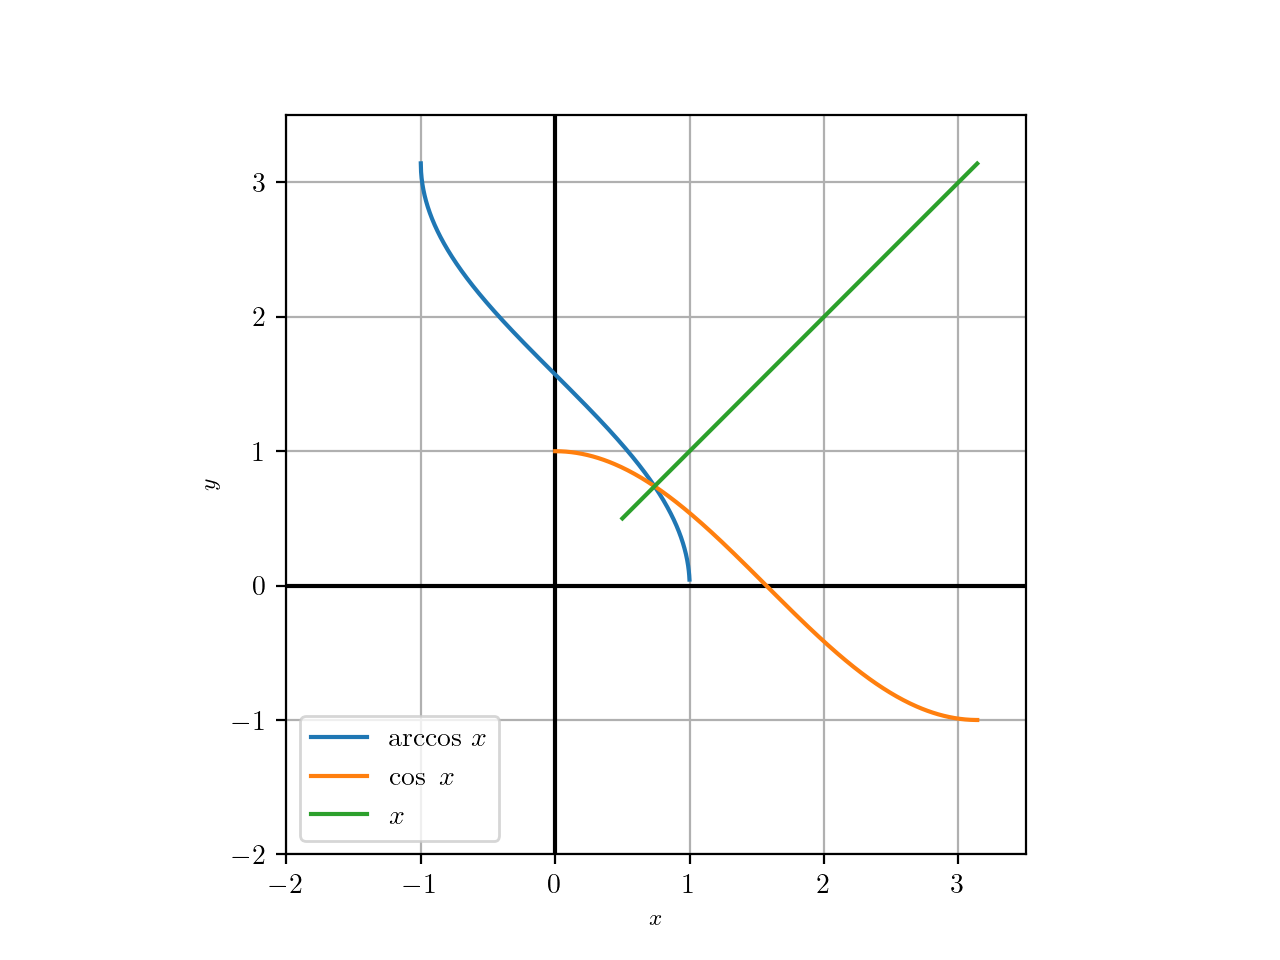
\includegraphics[scale=0.7]{arccos.png}
  \caption{Tracé de arccosinus}
  \label{fig:tracearccosinus}
\end{figure}
%
\begin{prop}
  Soit un réel \(x\) de \(\intervalleff{-1}{1}\), alors on a
  \begin{gather}
    \cos( \arcsin x)=\sin( \arccos x)=\sqrt{1-x^2}; \\
    \arccos x + \arcsin x = \frac{\pi}{2};\\
    \arccos(-x) = \pi - \arccos x.
  \end{gather}
\end{prop}
\begin{proof}
  \begin{itemize}
  \item puisque \(\arcsin x \in \intervalleff{-\frac{\pi}{2}}{\frac{\pi}{2}}\) alors
    \begin{equation}
      \cos( \arcsin x)=\sqrt{1- \sin^2(\arcsin x)}=\sqrt{1-x^2} \geqslant 0
    \end{equation}
    On fait le même raisonnement avec \(\arccos x\).
  \item On sait aussi que
    \begin{equation}
      \cos( \arccos x) = x = \sin( \arcsin x)=\cos \left( \frac{\pi}{2} - \arcsin x \right),
    \end{equation}
    et puisque \(\cos\) est bijective sur \(\intervalleff{0}{\pi}\), on a égalité.
  \item De la même manière
    \begin{equation}
      \cos( \arccos -x)=-x=-\cos( \arccos x)=\cos(\pi - \arccos x),
    \end{equation}
    et comme cosinus est bijectif dans \(\intervalleff{0}{\pi}\), on en déduit l'égalité.
  \end{itemize}
\end{proof}
%
\subsection{Fonction arctangente}
\label{subsec:chap1-fonctionarctangente}
\begin{defdef}
  La restriction de la fonction tangente à l'intervalle \(\intervalleoo{-\frac{\pi}{2}}{\frac{\pi}{2}}\) est une bijection~\footnote{Idem}, sa réciproque est la fonction arctangente notée \(\arctan\).
\end{defdef}
\begin{prop}
  Soit un réel \(x\) quelconque et un réel \(y\) non nul. Alors
  \begin{gather}
    \cos(\arctan x)=\frac{1}{\sqrt{1+x^2}};\\
    \sin(\arctan x)=\frac{x}{\sqrt{1+x^2}};\\
    \arctan y + \arctan \frac{1}{y} = \sgn(y) \frac{\pi}{2}.
  \end{gather}
\end{prop}
\begin{proof}
  Soit un réel \(x\) quelconque et un réel \(y\) non nul, alors
  \begin{itemize}
  \item puisque \(-\frac{\pi}{2} < \arctan x < \frac{\pi}{2}\) alors \(\cos(\arctan x)>0\) donc
    \begin{equation}
      \cos(\arctan x)=\sqrt{\cos^2(\arctan x)}=\sqrt{\frac{1}{1+\tan^2(\arctan x)}}=\frac{1}{\sqrt{1+x^2}};
    \end{equation}
  \item de la même manière on a
    \begin{equation}
      \cos(\arctan x)=\sin( \arctan x) \tan(\arctan x) = \frac{x}{\sqrt{1+x^2}};
    \end{equation}
  \item soit la fonction \(\fonction{f}{\Rplusetoile}{\R}{y}{\arctan y + \arctan \frac{1}{y}}\) dérivable et pour tout réel \(y\) positif, on a
    \begin{equation}
      f'(y)=\frac{1}{1+y^2} - \frac{1}{y^2} \cdot \frac{1}{1+\frac{1}{y^2}}=0.
    \end{equation}
    La fonction \(f\) est donc constante et en \(y=1\) on a \(f(1)=\frac{\pi}{2}=f(y)\). Si \(y\) est strictement négatif, alors comme \(\arctan\) est impaire, on a \(f(y)=-\frac{\pi}{2}\).
\end{itemize}
\end{proof}
%
\begin{figure}
  \centering
  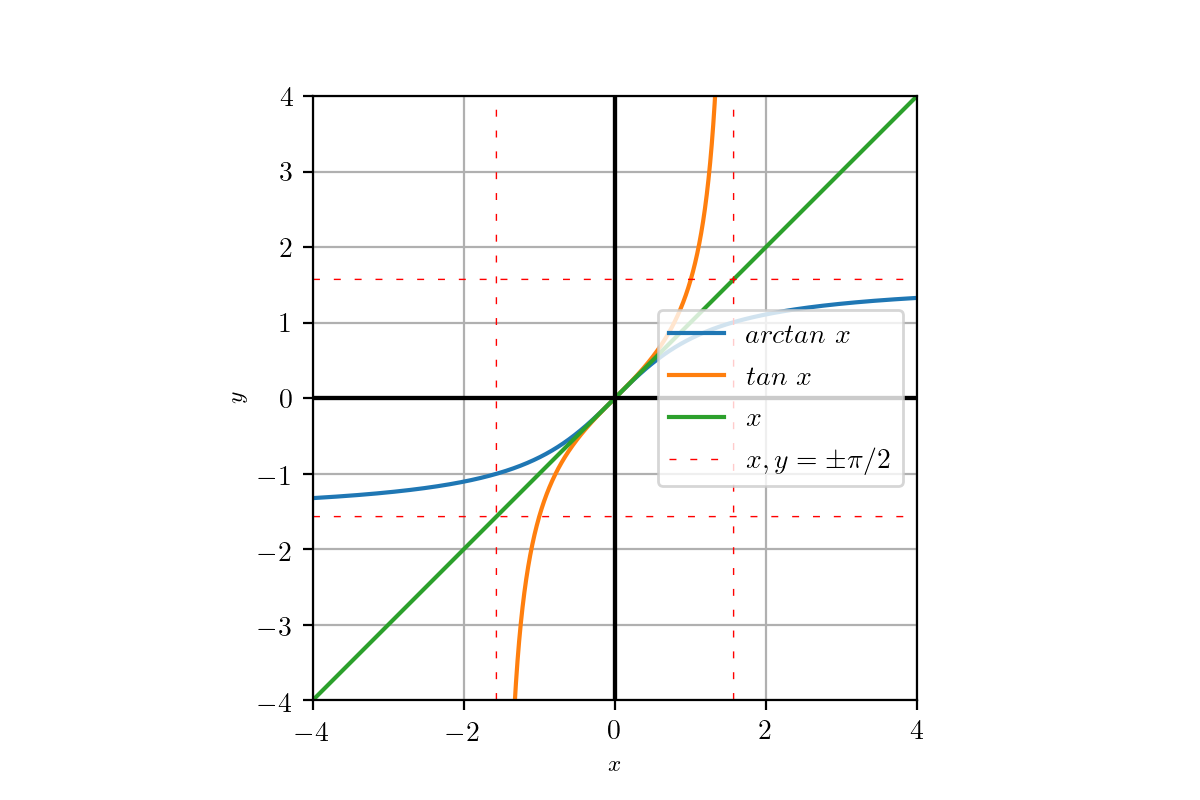
\includegraphics[scale=0.7]{arctan.png}
  \caption{Tracé de arctangente et de ses asymptotes}
  \label{fig:tracearctangente}
\end{figure}
%
\begin{theo}
  \label{chap1-theo:thetasin}
  Soient des réels \(x\) et \(y\) tels que \(x^2+y^2=1\), alors il existe un unique réel \(\theta\) dans \(\intervalleof{-\pi}{\pi}\) tel que \(x=\cos \theta\) et \(y=\sin \theta\).
\end{theo}
\begin{proof}[Existence]
  On sait que \(x^2=1-y^2\) avec \(x^2 \in \intervalleff{0}{1}\) donc \(x \in \intervalleff{-1}{1}\). On peut donc définir un \(\theta_0=\arccos x \in \intervalleff{0}{\pi}\) tel que \(x=\cos \theta_0\). Ainsi \(y^2=1-x^2=\sin^2 \theta_0\). Puisque \(\theta_0 \in \intervalleff{0}{\pi}\) on a \(\sin \theta_0>0\) alors \(\abs{y}=\sin \theta_0\).
Si \(y \geqslant 0\) et comme \(\theta_0 \in \intervalleff{0}{\pi}\), alors \(\theta=\theta_0\) est le bon réel.

Mais si \(y<0\), alors on prend l'opposé \(\theta=-\theta_0 \in \intervalleof{-\pi}{0}\).

On a bien montré l'existence d'un réel \(\theta \in \intervalleof{-\pi}{\pi}\) tel que \(x=\cos \theta\) et \(y=\sin \theta\).
\end{proof}
\begin{proof}[Unicité]
  Supposons qu'il existe deux réel \(\theta\) et \(\theta'\) tels que
  \begin{equation}
    \begin{cases} x=\cos \theta = \cos \theta' \\ y=\sin \theta = \sin \theta' \end{cases},
  \end{equation}
  alors \(x=\cos \abs{\theta}=\cos \abs{\theta'}\) puisque la fonction cosinus est paire. Les réels \(\abs{\theta}\) et \(\abs{\theta'}\) sont dans \(\intervalleff{0}{\pi}\). La restriction de cosinus à \(\intervalleff{0}{\pi}\) est bijective, on en déduit que \(\abs{\theta}=\abs{\theta'}\). Deux cas se présentent~:
  \begin{itemize}
  \item Soit \(\theta'=\theta\);
  \item Soit \(\theta'=-\theta\) et alors \(\sin \theta = \sin \theta' = -\sin \theta\) donc \(\sin \theta = 0\) ainsi, \(\theta = 0\) ou \(\theta = \pi\). Comme \(\theta'=-\theta \in \intervalleof{-\pi}{\pi}\) on a forcément \(\theta = 0 = \theta'\).
\end{itemize}
\end{proof}
%
\section{Trigonométrie hyperbolique}
\label{sec:chap1-trigohyper}
\subsection{Fonctions sinus et cosinus hyperbolique}
\label{subsec:chap1-sinushetcosh}
\begin{defdef}
  On définit les applications de \(\R\) dans \(\R\), appelées respectivement sinus et cosinus hyperbolique, notée \(\hsin\) et \(\hcos\), par
  \begin{gather}
    \forall x \in \R \quad \hsin x = \frac{\e^x - \e^{-x}}{2}, \\
    \forall x \in \R \quad \hcos x = \frac{\e^x + \e^{-x}}{2}.
  \end{gather}
\end{defdef}
%
\begin{prop}
  La fonction sinus hyperbolique est impaire et cosinus hyperbolique est paire. Les fonctions sinus hyperbolique et cosinus hyperbolique sont dérivables sur \(\R\) avec \(\hsin'=\hcos\) et \(\hcos'=\hsin\).
\end{prop}
\begin{proof}
  \(\R\) est centré en \(0\) et ---~grâce aux calculs~--- \(\hsin(-x)=-\hsin x\) et \(\hcos(-x)=\hcos x\). La fonction exponentielle est dérivable sur \(\R\), donc \(\hsin\) et \(\hcos\) sont dérivables et les calculs donnent bien la formule.
\end{proof}
%
\begin{prop} Soit un réel \(x\), alors
\begin{gather}
  \hcos x + \hsin x = \e^x, \\
  \hcos x - \hsin x = \e^{-x}, \\
  \hcos^2 x - \hsin^2 x = 1.
\end{gather}
\end{prop}
\begin{proof}
  Ces formules sont des conséquences de la définition.
\end{proof}
%
\begin{figure}
  \centering
  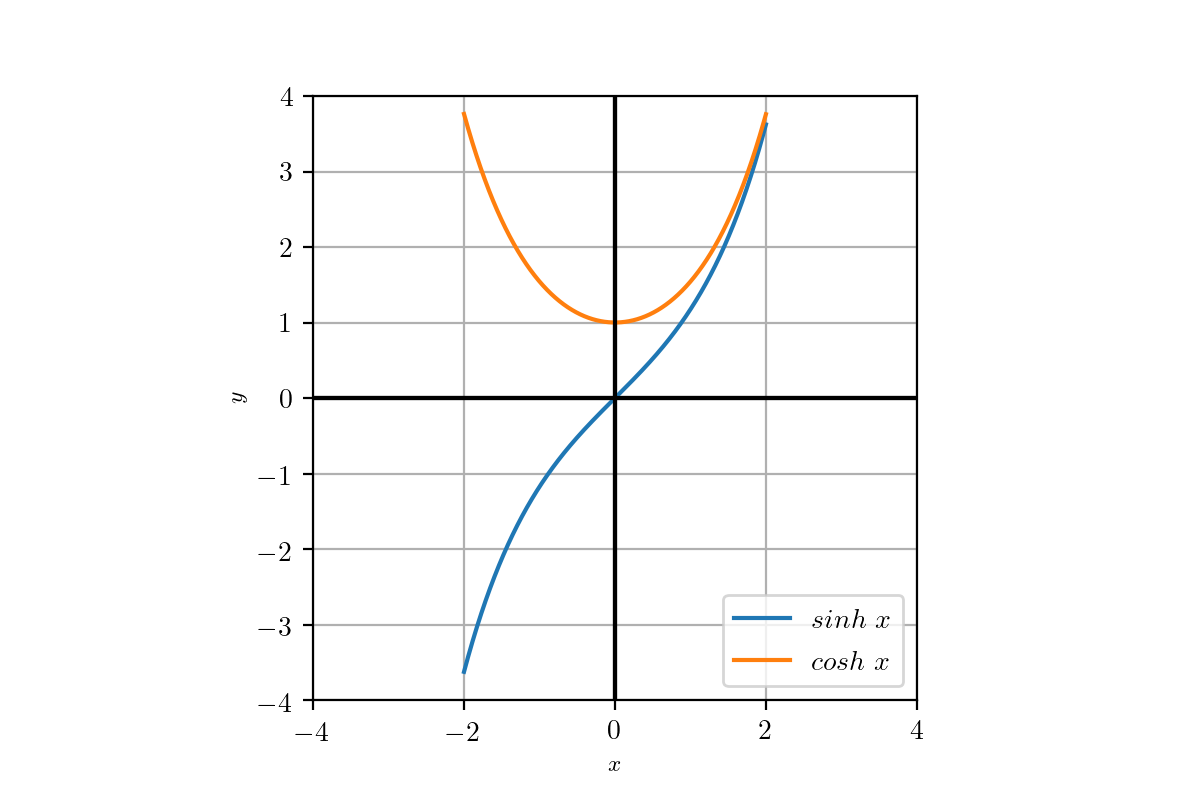
\includegraphics[scale=0.7]{trigh.png}
  \caption{Tracé de fonctions hyperbolique \(\hsin\) et \(\hcos\)}
  \label{fig:tracesinhcosh}
\end{figure}
%
Les fonctions \(\hsin\) et \(\hcos\) permettent de paramétrer l'hyperbole \(\mathcal{H}\) d'équation~: \(\frac{x^2}{a^2} - \frac{y^2}{b^2}=1\)  par \(\begin{cases} x(t)=a \epsilon \hcos t \\ y(t)=b \epsilon \hsin t\end{cases} \epsilon \in \intervalleff{-1}{1}\), d'où le nom de ces fonctions.
%
\subsection{Fonctions tangente et cotangente hyperbolique}
\label{subsec:chap1-tanhetcotanh}
\begin{defdef}
  On définit la tangente hyperbolique, noté \(\htan\), et la cotangente hyperbolique, notée \(\hcotan\), comme
  \begin{gather}
    \forall x \in \R \quad \htan(x)=\frac{\hsin x}{\hcos x}=\frac{\e^x - \e^{-x}}{\e^x+\e^{-x}}, \\
    \forall x \in \R^* \quad \hcotan(x)=\frac{\hcos x}{\hsin x}=\frac{\e^x + \e^{-x}}{\e^x-\e^{-x}}.
  \end{gather}
\end{defdef}
%
\begin{prop}
  Les fonctions tangente et cotangente hyperbolique sont impaires. Elles sont dérivables sur leurs ensembles de définition respectifs et on a
  \begin{equation}
    \forall x \in \R \quad \htan' x = 1-\htan^2 x = \frac{1}{\hcos^2 x}
  \end{equation}
  et
  \begin{equation}
    \forall y \in \Rplusetoile \quad \hcotan' x=1-\hcotan^2 x=-\frac{1}{\hsin^2 x}.
  \end{equation}
\end{prop}
\begin{proof}
  \(\R\) est centré en zéro et on vérifie que
  \begin{gather}
    \htan(-x)=-\htan x, \\
    \hcotan(-x) = -\hcotan x.
  \end{gather}
  Ensuite puisque \(\hsin\) et \(\hcos\) sont dérivables sur \(\R\) et puisque \(\hcos\) ne s'annule pas sur \(\R\), on a pour tout réel \(x\)
  \begin{equation}
    \htan' x = \frac{\hcos^2 x - \hsin^2 x}{\hcos^2 x},
  \end{equation}
  qui nous donne la formule. De la même manière \(\sinh\) ne s'annule qu'en \(x=0\) donc pour \(x\) non nul, on a la formule
  \begin{equation}
    \hcotan' x = \frac{\hsin^2 x - \hcos^2 x}{\hsin^2 x},
  \end{equation}
  qui nous donne aussi la formule.
\end{proof}
La fonction tangente hyperbolique est strictement croissante et la cotangente décroît sur \(\Rmoinsetoile\) et sur \(\Rplusetoile\).
%
\begin{figure}
  \centering
  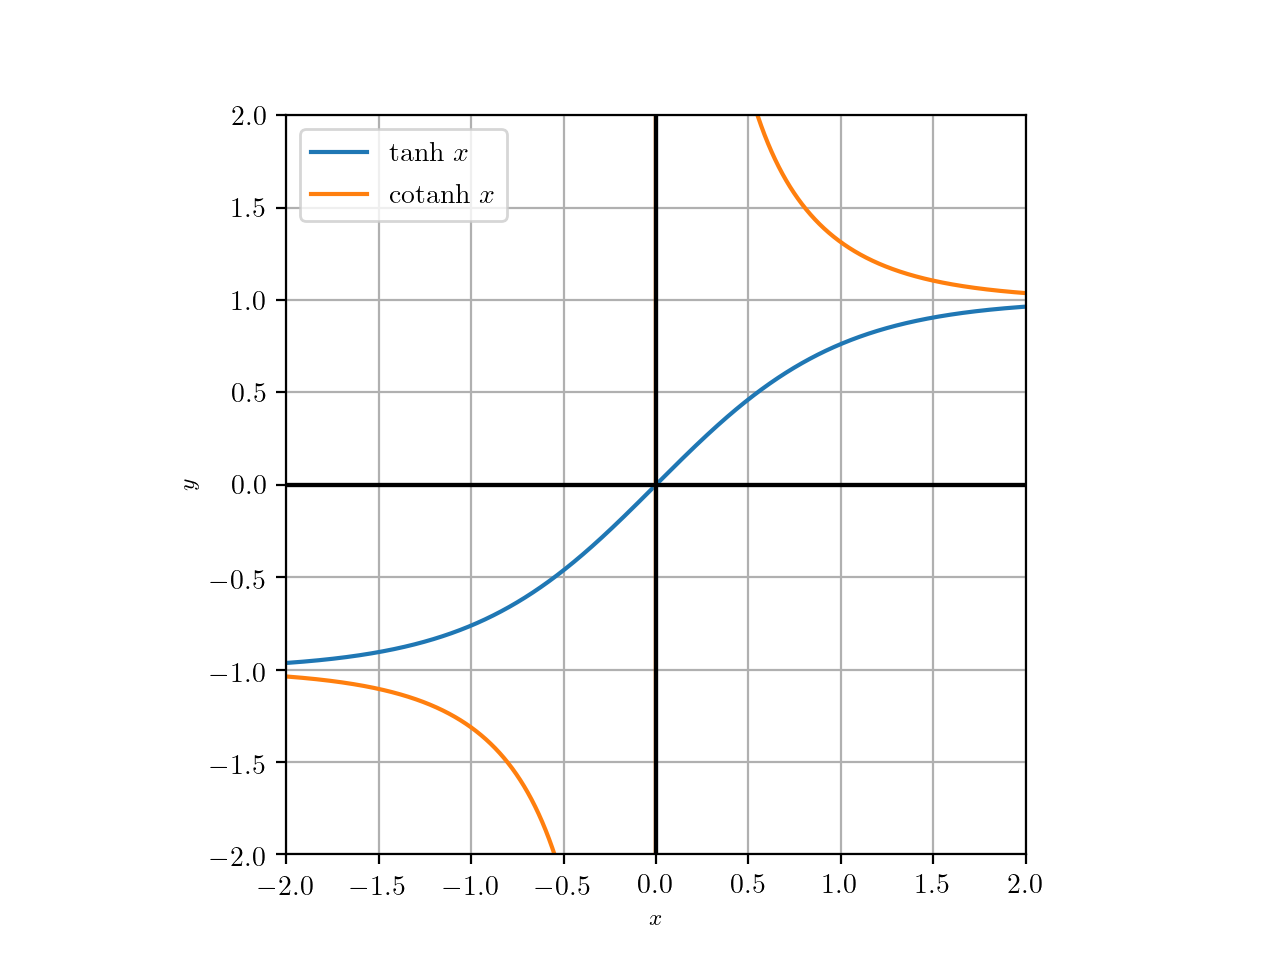
\includegraphics[scale=0.7]{tanh.png}
  \caption{Tracé de fonctions hyperbolique \(\htan\) et \(\hcotan\)}
  \label{fig:tracetanhcoth}
\end{figure}
%
\subsection{Formulaire de trigonométrie hyperbolique}
\label{subsec:chap1-formulairetrigohyp}
En théorie la seule formule exigible est \(\hcos^2-\hsin^2=1\) mais les autres existent, elles peuvent se retrouver à partir du formulaire de trigonométrie circulaire en remplaçant \(\cos\) par \(\hcos\) et \(\sin\) par \(\ii \hsin\).
%
\section{Fonctions hyperboliques réciproques}
\label{sec:chap1-fonctionshyprec}
\subsection{Fonction argument sinus hyperbolique}
\label{subsec:chap1-fonctionargsinh}
\begin{defdef}
  La fonction sinus hyperbolique est une bijection de \(\R\) sur lui-même et admet une réciproque appelée argument sinus hyperbolique notée \(\argsh\).
\end{defdef}
%
\begin{prop}
  \begin{equation}
    \forall x, y \in \R \quad y=\hsin x \iff x=\argsh y.
  \end{equation}
\end{prop}
%
\begin{prop}
La fonction \(\argsh\) est impaire et strictement croissante.
\end{prop}
\begin{proof}
  Soit un réel \(x\), alors
  \begin{equation}
    x=\hsin (\argsh x)=-\hsin(-\argsh x),
  \end{equation}
  donc
  \begin{equation}
    -x=\hsin(\argsh -x)=\hsin(-\argsh x).
  \end{equation}
  Comme la fonction sinus hyperbolique est bijective, on a bien l'égalité
  \begin{equation}
    \argsh(-x)=-\argsh x,
  \end{equation}
  et comme \(\R\) est centré en zéro, alors \(\argsh\) est impaire.
\end{proof}
%
\begin{prop}
  La fonction argument sinus hyperbolique est dérivable sur \(\R\) et pour tout réel \(x\), on a
  \begin{equation}
    \argsh' x= \frac{1}{\sqrt{1+x^2}}.
  \end{equation}
\end{prop}
\begin{proof}
  La fonction sinus hyperbolique est dérivable sur \(\R\) et
  \begin{equation}
    \forall y \in \R \quad \hsin' (\argsh y)=\hcos(\argsh y)>0,
  \end{equation}
  donc la fonction argument sinus hyperbolique est dérivable en \(y\) et
  \begin{equation}
    \argsh' y =\frac{1}{\hcos( \argsh y)}=\frac{1}{\sqrt{1+\hsin^2(\argsh y)}}=\frac{1}{\sqrt{1+y^2}}.
  \end{equation}
\end{proof}
%
\begin{prop}[Expression logarithmique]
La fonction argument sinus hyperbolique peut s'exprimer ainsi
 \begin{equation}
   \forall x \in \R \quad \argsh x = \ln(x+\sqrt{1+x^2}).
 \end{equation}
\end{prop}
\begin{proof}
  Soient deux réels \(x\) et \(y\) tels que \(y=\argsh x\) alors \(x=\frac{\e^y - \e^{-y}}{2}\). C'est-à-dire
  \begin{equation}
    \e^y - \e^{-y} -2x=0,
  \end{equation}
  soit
  \begin{equation}
    \e^{2y}-1-2x\e^{y}=0.
  \end{equation}
  Les solutions réelles de l'équation \(Y^2-2xY-1=0\) sont \(x-\sqrt{x^2+1}<0\) et \(x+\sqrt{x^2+1}\) et donc \(\e^y=x+\sqrt{x^2+1}\) soit pour finir l'expression logarithmique
  \begin{equation}
    \argsh x = y = \ln(x+\sqrt{x^2+1}).
  \end{equation}
\end{proof}
%
\begin{figure}
  \centering
  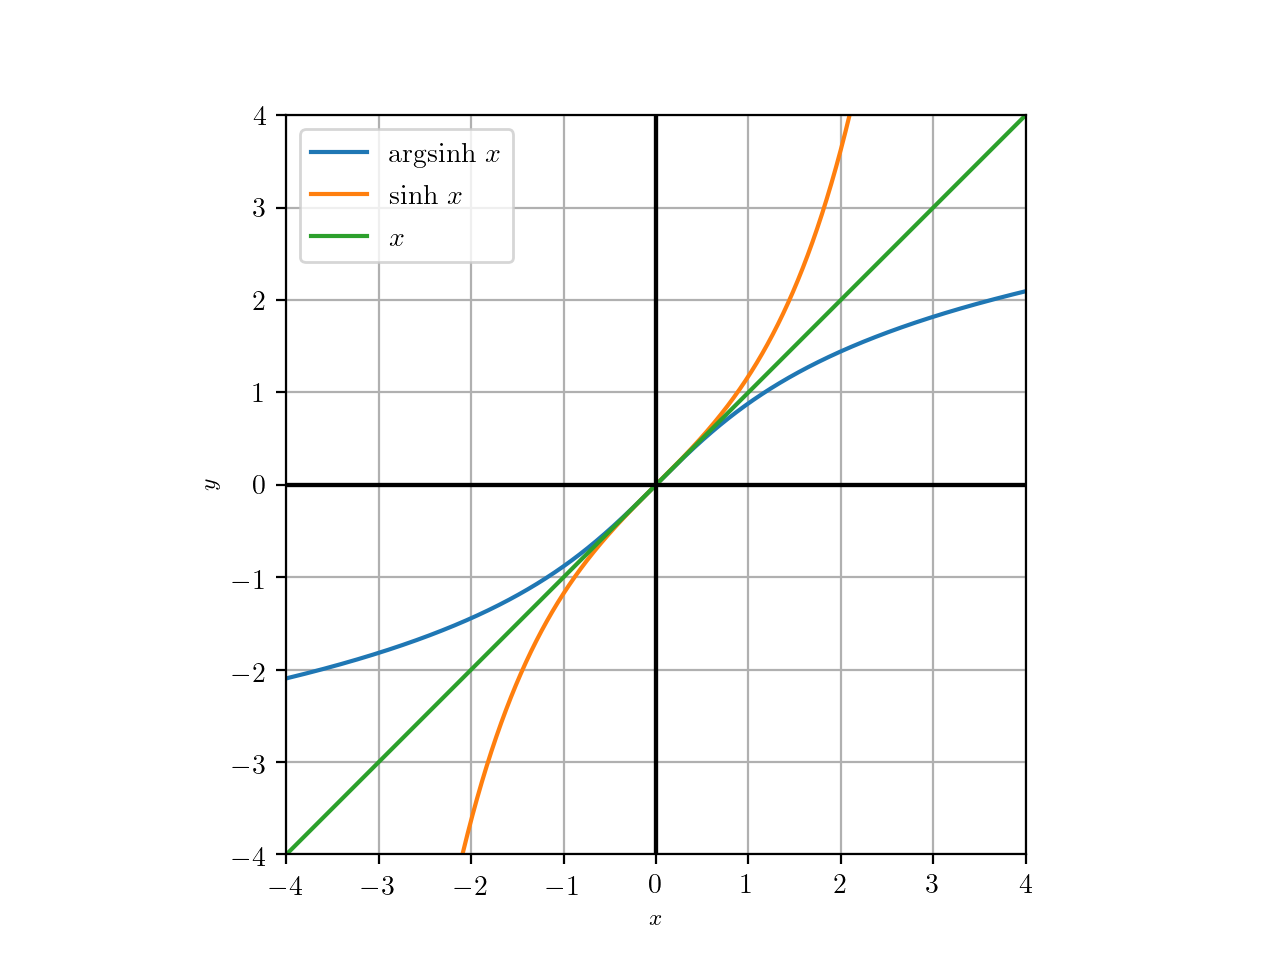
\includegraphics[scale=0.7]{argsinh.png}
  \caption{Tracé de fonctions hyperbolique \(\hsin\) et \(\argsh\)}
  \label{fig:tracesinhargsh}
\end{figure}
%
\subsection{Fonction argument cosinus hyperbolique}
\label{subsec:chap1-fonctionargcosh}
\begin{defdef}
  La fonction cosinus hyperbolique induit une bijection de \(\Rplus\) sur \(\intervallefo{1}{+\infty}\) qui admet une réciproque appelée argument cosinus hyperbolique et notée \(\argch\).
\end{defdef}
%
\begin{prop}
  \begin{equation}
    \forall x \in \Rplus \ \forall y \in \intervallefo{1}{+\infty} \quad y=\hcos x \iff x = \argch y ;
  \end{equation}
  et on a
  \begin{gather}
    \forall y \in \intervallefo{1}{+\infty} \quad \hcos(\argch y) = y, \\
    \forall x \in \Rplus \quad \argch(\hcos x) = x.
  \end{gather}
\end{prop}
%
\begin{prop}
  La fonction argument cosinus hyperbolique est strictement croissante et est dérivable sur son domaine de définition telle que
  \begin{equation}
    \forall x\geqslant{}1 \quad \argch' x =\frac{1}{\sqrt{x^2-1}}.
  \end{equation}
\end{prop}
\begin{proof}
  Puisque la fonction cosinus hyperbolique est dérivable sur \(\Rplus\) et que \(\hsin(\argch y) \neq 0\) On tire que \(\argch\) n'est pas dérivable en un~: \(\hcos'(\argch 1)=0\) la courbe admet une tangente verticale. Si \(y>1\), alors \(\argch\) est dérivable en \(y\) et
  \begin{equation}
    \argch'(y)=\frac{1}{\hsin(\argch y)}=\frac{1}{\sqrt{\hcos^2(\argch y)-1}}=\frac{1}{\sqrt{y^2-1}}.
  \end{equation}
\end{proof}
%
\begin{prop}[Expression logarithmique] La fonction argument cosinus hyperbolique peut s'exprimer telle que
  \begin{equation}
    \forall x>1 \quad \argch x = \ln \left(x +\sqrt{x^2-1}\right).
  \end{equation}
\end{prop}
\begin{proof}
  \begin{equation}
    \forall x \in \Rplus \ \forall y \in \intervallefo{1}{+\infty} \quad x=\argch y \iff y=\hsin x.
  \end{equation}
  Soit donc en remplaçant \(\hcos\) par son expression
  \begin{equation}
    \e^{2x} +1 - 2y\e^x =0.
  \end{equation}
  Ainsi \(\e^x\) est solution de \(X^2-2yX+1=0\) soit \(\e^x = y \pm \sqrt{y^2-1}\). En choisissant la solution supérieure à un on obtient \(x=\ln \left(y+\sqrt{y^2-1} \right)\).
\end{proof}
%
\begin{figure}
  \centering
  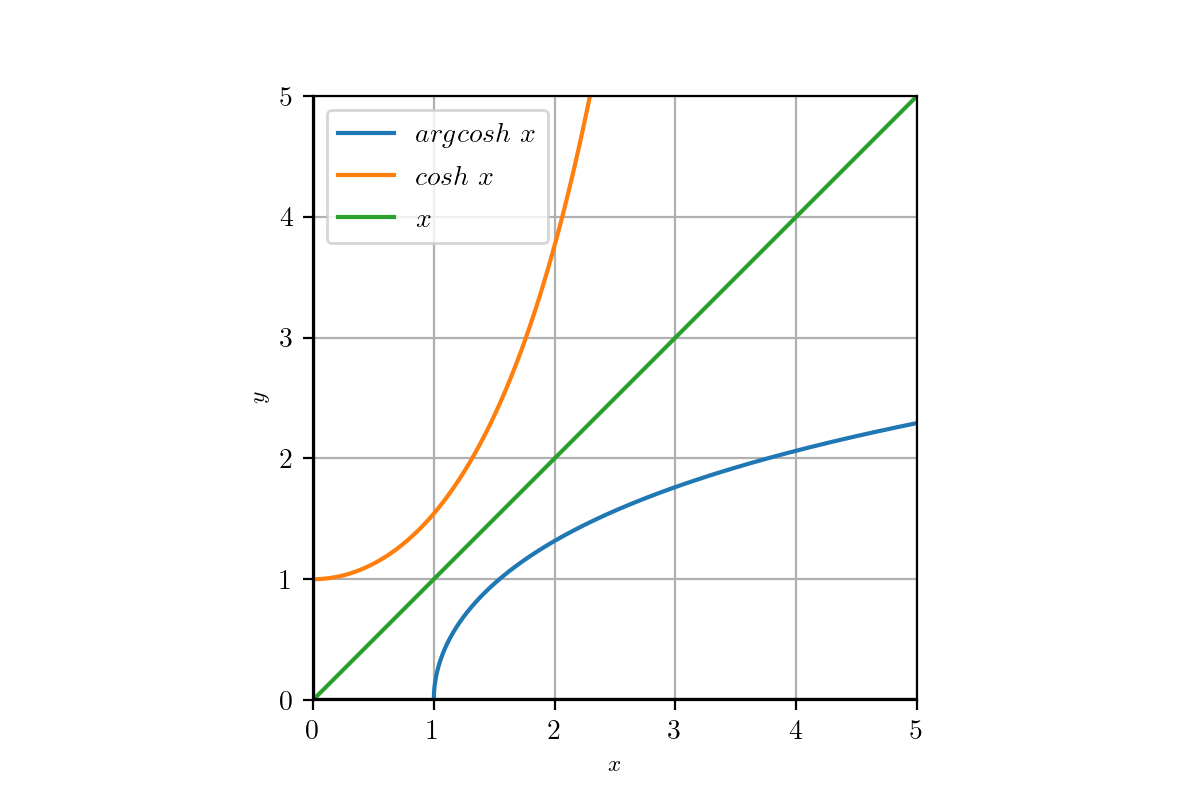
\includegraphics[scale=0.7]{argcosh.png}
  \caption{Tracé de fonctions hyperbolique \(\hcos\) et \(\argch\)}
  \label{fig:tracecoshargcosh}
\end{figure}
%
\subsection{Fonction argument tangente hyperbolique}
\label{subsec:chap1-fonctionargtanh}
\begin{defdef}
  La fonction tangente hyperbolique induit une bijection de \(\R\) sur \(\intervalleoo{-1}{1}\). Elle admet donc une réciproque appelée argument tangente hyperbolique notée \(\argth\).
\end{defdef}
%
\begin{prop}
  Pour tous réel \(x\) et \(y\) de \(\intervalleoo{-1}{1}\), on a
  \begin{gather}
    y=\htan x \iff x= \argth x, \\
    \argth(\htan x)=x, \\
    \htan(\argth y)=y.
  \end{gather}
\end{prop}
%
\begin{prop}
  La fonction argument tangente hyperbolique est impaire et strictement croissante.
\end{prop}
%
\begin{prop}
  La fonction argument tangente hyperbolique est dérivable sur son ensemble de définition telle que
  \begin{equation}
    \forall x \in \intervalleoo{-1}{1} \quad \argth'(x)=\frac{1}{1-x^2}.
  \end{equation}
\end{prop}
\begin{proof}
  Puisque tangente hyperbolique est dérivable sur \(\R\) et que
  \begin{equation}
    \htan'(\argth y)=1-\htan^2(\argth y)=1-y^2>0,
  \end{equation}
  alors la fonction \(\argth\) est dérivable et la formule est donnée.
\end{proof}
%
\begin{prop}[Expression logarithmique]
  La fonction argument tangente hyperbolique peut s'écrire telle que
  \begin{equation}
    \forall y \in \intervalleoo{-1}{1} \quad \argth y =\frac{1}{2} \ln \left( \frac{1+y}{1-y} \right).
  \end{equation}
\end{prop}
\begin{proof}
  \begin{equation}
    \forall (x,y) \in \R \times \intervalleoo{-1}{1} \quad y=\htan x = \frac{\e^{2x}-1}{\e^{2x}+1},
  \end{equation}
  de la même manière on arrive à une équation du deuxième degré~:
  \begin{equation}
    \e^{2x} = \frac{1+y}{1-y} ,
  \end{equation}
  et puisque \(-1<y<1\), on peut passer au logarithme et on obtient la formule.
\end{proof}
%
\begin{figure}
  \centering
  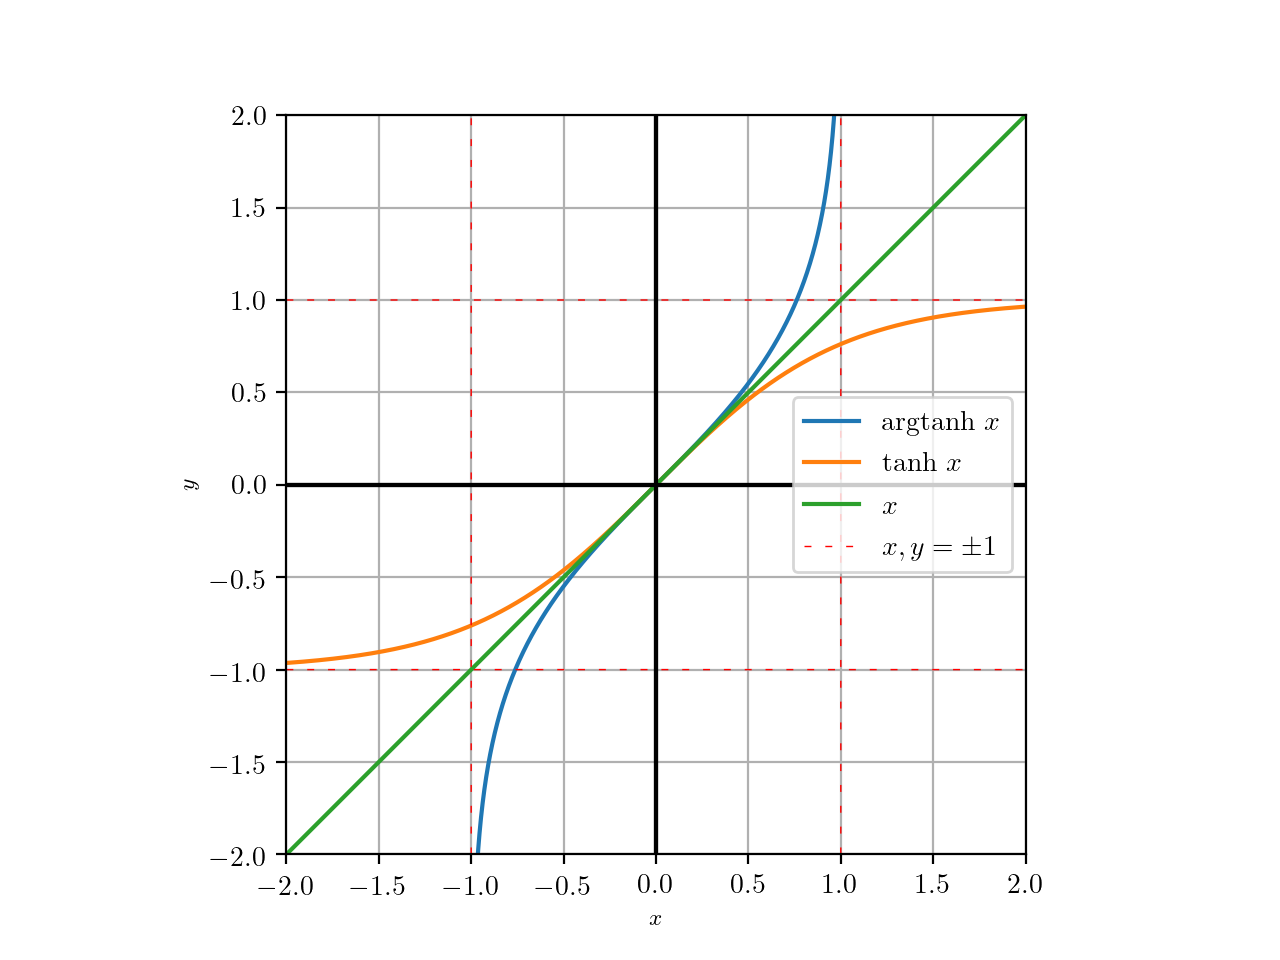
\includegraphics[scale=0.7]{argtanh.png}
  \caption{Tracé des fonctions hyperbolique \(\htan\) et \(\argth\) et de leurs asymptotes}
  \label{fig:tracetanhargth}
\end{figure}
\cleardoublepage
\section{Exercices}
\subsection{Fonctions logarithme, exponentielle et puissance}
\begin{exercice}
    Soit \(a > 1\) et \(\alpha \in \R\).
    \begin{itemize}
        \item Discuter le nombre de racines sur \(\intervalleoo{0}{+\infty}\) de l'équation~:
            \begin{equation}
                \label{eq:fiche1-1}
                a^x = x^\alpha
            \end{equation}
        \item Démontrer que l'équation~:
            \begin{equation}
                a^{a^x} = x
            \end{equation}
            a les mêmes racines que l'équation~:
            \begin{equation}
                a^x = x.
            \end{equation}
            En déduire le nombre de racines de l'équation \eqref{eq:fiche1-1}.
    \end{itemize}
\end{exercice}
\begin{exercice}
    Résoudre sur \(\intervalleoo{0}{+\infty}\) le système d'équations aux inconnues \(x\) et \(y\) suivant~:
    \begin{equation}
       \begin{cases} 7(\log_y x +\log_x y) = 50 \\ xy = 256 \end{cases} 
    \end{equation}
\end{exercice}
\begin{exercice}
    Comparer \(\e^\pi\) et \(\pi^e\).
\end{exercice}
\begin{exercice}
    Soit, pour tout réel \(\alpha\) et tout naturel \(n\) non nul la fonction \(f_{alpha, n}\), notée par la suite $f$, définie pour tout \(x>0\), \(f_{\alpha, n}(x) = x^\alpha (\ln x)^n \).
    \begin{enumerate}
        \item Étudier la fonction \(f\) au voisinage de ses bornes
        \item Étudier les variations de \(f\)
        \item Représenter graphiquement \(f\). \emph{Attention, on devra trouver 15 représentations graphiques distinctes, en fonction de la valeur de \(n\) et de \(\alpha\).}
    \end{enumerate}
\end{exercice}
\begin{exercice}
    Résoudre dans \(\R\) les équations suivantes~:
    \begin{align}
        (\sqrt{x})^x &= x^{\sqrt{x}} \\
        2\ln x + \ln(2x-1) &= \ln(2x+8) + 2\ln(x-1) \\
        \e^{2x} -2\e^x-3 &=0 \\
        \sqrt{x+4-4\sqrt{x}} + \sqrt{x+9-6\sqrt{x}} &= 1
    \end{align}
\end{exercice}
\subsection{Fonctions circulaires, hyperboliques et leurs réciproques}
\begin{exercice}
    Résoudre sur \(\R\) l'équation~:
    \begin{equation}
        \frac{\sin x + \sin 2x + \sin 3x}{\cos x + \cos 2x + \cos 3x} = 1
    \end{equation}
\end{exercice}
\begin{exercice}
    Soit la fonction \(f\) telle que~:
    \begin{equation}
        f(x) = (\sqrt{1-\sin 2x}+\sqrt{1+\sin 2x})^{\frac{1}{\ln(\cos 2x)}}
    \end{equation}
    \begin{enumerate}
        \item Quel est le domaine de définition de \(f\) ?
        \item Démontrer que quelque soit le réel \(x\), \(\sqrt{1-\sin 2x}=\abs{\sin x - \cos x}\).
        \item Étudier la parité et la périodicité de \(f\)
        \item Trouver une expression de \(f\) plus simple sur \(\intervallefo{0}{\pi/2}\setminus\{\pi/3\}\).
        \item Étudier les variations de \(f\) et la représenter graphiquement.
    \end{enumerate}
\end{exercice}
\begin{exercice}
    Résoudre sur \(\R\) l'équation
    \begin{equation}
        2\arcsin x = \arcsin(2x\sqrt{1-x^2})
    \end{equation}
\end{exercice}
\begin{exercice}
    Déterminer pour tout réel \(a\) et tout naturel \(n\) une expression simple de la somme~:
    \begin{equation}
        S_n = \sum_{k=1}^n 2^k \tanh(2^k a
    \end{equation}
    \emph{Indication :} On pourra essayer de simplifier l'expression~:
    \[\frac{2}{\tanh 2x} - \frac{1}{\tanh x}\]
\end{exercice}
\begin{exercice}
    Déterminer, pour tout réel \(x\) de l'intervalle \(\intervallefo{0}{\pi/2}\) et tout naturel \(n\), une expression simple du réel~:
    \begin{equation}
        \sum_{k=0}^{n-1} \frac{\cos kx}{\cos^k x}
    \end{equation}
\end{exercice}
\begin{exercice}
    Déterminer si elles existent les limites~:
    \begin{align}
        \lim\limits_{x \to +\infty} 2\cosh^2x-\sinh 2x \\
        \lim\limits_{x \to +\infty} \e^{2x}(2\cosh^2x-\sinh 2x)
    \end{align}
\end{exercice}
\begin{exercice}
    Soient \(y \in \intervalleoo{0}{\pi/2}\) et \(x = \ln\tan(\pi/4+y/2)\). Exprimer en focntion de \(y\) chacun des réels \(\tanh(x/2), \sinh x, \cosh x\) et \(\tanh x\).
\end{exercice}
\begin{exercice}
    Démontrer que pour tout réels \(a\) et \(b\) strictement compris entre \(-1\) et \(1\),
    \begin{equation}
        \argth a + \argth b = \argth \frac{a+b}{1+ab}
    \end{equation}
\end{exercice}
\begin{exercice}
    Soient \(a\) et \(b\) deux réels. Résoudre sur \(\R\) le système suivant~:
    \begin{equation}
        \begin{cases} \cosh x \cosh y = a \\ \sinh x \sinh y = b \end{cases}
    \end{equation}
\end{exercice}
\begin{exercice}
    Étudier et représenter graphiquement les fonctions \(f\) suivantes~:
    \begin{align}
        f(x) &= \arcsin \sin x \\
        f(x) &= \argch \sqrt{\frac{1+\cosh x}{2}} \\
        f(x) &= \arccos(4x^3-3x) \\
        f(x) &= \argth\sqrt{\frac{\cosh x - 1}{\cosh x + 1}}
    \end{align}
\end{exercice}
\begin{exercice}
    Soit un réel \(x\), simplifier l'expression~:
    \begin{equation}
        \arccos \cos x + 1/2 \arccos\cos 2x + 1/6\arccos\cos 3x
    \end{equation}
\end{exercice}
\begin{exercice}
    Soit un réel \(x\), comparer \(\cos\sin x\) et \(\sin\cos x\).
\end{exercice}

\chapter{Nombres complexes}
\label{chap:complexes}
\minitoc
\minilof
\minilot

Les nombres complexes sont présentés dans ce chapitre. L'ensemble des nombres complexes forme une extension de l'ensemble des nombres réels. Les complexes permettent notamment de définir des solutions à toutes les équations polynomiales à coefficients réels.

La première section se focalise sur leur définition et leurs propriétés. On s'intéresse ensuite à la trigonométrie en utilisant les complexes. Les équations du second degré sont ensuite résolues grâce aux complexes. L'exponentielle complexe est ensuite présentée puis l'application des complexes en géométrie plane est exposée.

\section{Corps des nombres complexes}
\label{sec:corpsdescomplexes}
La construction de ce corps est hors programme. On le définit tel quel.
\begin{defdef}
  L'ensemble des complexes est défini par
\begin{empheq}[box=\shadowbox*]{align}
%  \begin{equation}
    \C = \enstq{x+ \ii y}{(x,y)\in \R},
%  \end{equation}
\end{empheq}
  tel que \(\ii^2=-1\).
\end{defdef}
\emph{Remarque} L'unité imaginaire \(\ii\) est souvent notée \(j\) en physique (pour ne pas confondre avec l'intensité). L'ensemble des complexes est muni de deux lois :
\begin{itemize}
\item l'addition, notée \(+\);
\item la multiplication, notée \(\times\) ou \(\cdot\).
\end{itemize}
%
\begin{prop} Tous les réels sont complexes, c'est-à-dire~:
\begin{empheq}[box=\shadowbox*]{align}
%  \begin{equation}
    \R \subset \C.
%  \end{equation}
\end{empheq}
  Les lois de \(\R\) coïncident avec les lois sur \(\C\).
\end{prop}
%
\begin{prop}
    \emph{\((\C,+)\) est un groupe commutatif}. C'est-à-dire que~:
  \begin{itemize}
  \item la loi \(+\) est associative,
    \begin{equation}
      \forall (x,y,z) \in \C^3 \quad x+(y+z)=(x+y)+z;
    \end{equation}
  \item la loi \(+\) est commutative,
    \begin{equation}
      \forall (x,y) \in \C^2 \quad x+y=y+x;
    \end{equation}
  \item \(\C\) admet un neutre pour \(+\)~: c'est \(0\);
  \item tout élément de \(\C\) est inversible par \(+\) et l'opposé de tout complexe \(x\) et \(-x\).
  \end{itemize}
\end{prop}
%
\begin{prop}
    \emph{\((\C,+,\times)\) est un anneau commutatif}. C'est-à-dire que \((\C,+)\) est un groupe commutatif et que
  \begin{itemize}
  \item \(\times\) est associative;
  \item \(\times\) admet un élément neutre noté \(1\);
  \item \(\times\) est distributive sur \(+\)~:
    \begin{equation}
      \forall (a,b,c) \in \C^3 \quad a \times (b+c)=a \times b+ a \times c.
    \end{equation}
\end{itemize}
\end{prop}
%
\begin{prop}
  Pour tout complexe \(z \in \C\), il existe un unique couple de réels \((x,y) \in \R^2\) tel que \(z=x+\ii y\). C'est-à-dire que l'application \(\fonctionL{\varphi}{\R^2}{\C}{(x,y)}{x+\ii y}\) est bijective.
\end{prop}
\emph{Interprétation géométrique~:} L'application $\varphi$ peut être vue comme une ``correspondance'' entre $\C$ et le plan $\R^2$, voir la figure~\ref{fig:complexe}.
\begin{figure}
    \centering
    \includegraphics[scale=0.7]{./Complexes.png}
    \caption{Représentation géométrique des complexes}
    \label{fig:complexe}
\end{figure}
\begin{proof}[Unicité]
  S'il existe deux couples de réels \((x,y),(x',y')\) tels que
  \begin{equation}
    x'+\ii y'=x +\ii y,
  \end{equation}
  alors
  \begin{equation}
    \underbrace{(x-x')^2}_{\geqslant 0}=\underbrace{-(y'-y)^2}_{\leqslant 0}.
  \end{equation}
  Finalement
  \begin{equation}
    (x-x')^2=(y'-y)^2=0.
  \end{equation}
\end{proof}
\begin{proof}[Existence]
  Par définition de l'ensemble des complexes, pour un complexe \(z\) donné, il existe toujours un couple de réels qui lui est associé.
\end{proof}
%
On appelle le réel \(x\) la partie réelle du complexe \(z\), \(x=\Re(z)\) et on appelle le réel \(y\) la partie imaginaire du complexe \(z\), \(y=\Im(z)\).
%
\begin{prop}
  Soient des complexes \(z\) et \(z'\) puis un réel \(\lambda\), alors
  \begin{equation}
      \Re(z+z')=\Re(z)+\Re(z'), \quad \Im(z+z')=\Im(z)+\Im(z'), \quad \Re(\lambda z)=\lambda \Re(z), \quad \Im(\lambda z)=\lambda \Im(z).
  \end{equation}
\end{prop}
%
\emph{Un complexe n'a pas de signe}. On note \(\C^*=\C \setminus \{0\}\)
%
\subsection{Conjugaison de complexe}
\label{subsec:conjugaisoncomplexe}
\begin{defdef}
  Soit \(z=x+\ii y \in \C\) avec \((x,y)\in \R\), on définit son conjugué de \(z\) noté \(\bar{z}\) par \(\bar{z}=x- \ii y\).
\end{defdef}
Les conjugués de deux complexes sont représentés dans le plan complexe sur la figure \ref{fig:conjugueComplexe}.
\begin{figure}
    \centering
    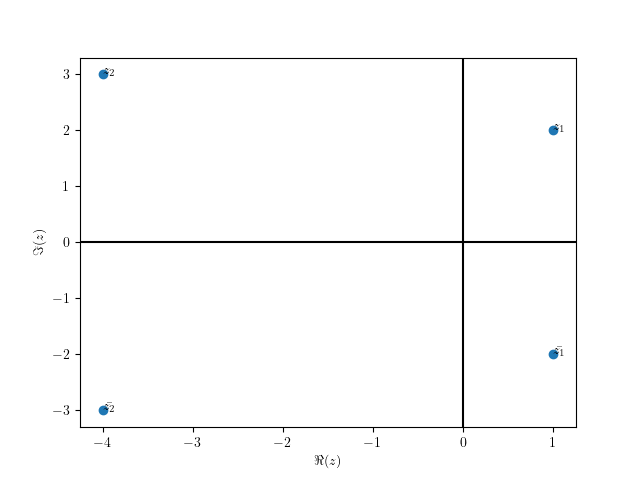
\includegraphics[scale=0.7]{conjugue.png}
    \caption{Représentation dans le plan complexe du conjugué de deux complexes $z_1$ et $z_2$}
    \label{fig:conjugueComplexe}
\end{figure}
%
\begin{prop}
  Soient des complexes \(z\) et \(z'\), alors
  \begin{equation}
      \bar{z+z'}=\bar{z} + \bar{z'}; \quad \bar{z \cdot z'}=\bar{z} \cdot \bar{z'}; \quad \bar{\bar{z}}=z.      
  \end{equation}
\end{prop}
\begin{prop}
  Pour tout complexe \(z\), on a
  \begin{equation}
      \Re(z)=\frac{z+\bar{z}}{2}; \quad \Im(z)=\frac{z-\bar{z}}{2 \ii}; \quad z \in \R \iff z=\bar{z}; \quad
      z \in \ii\R \iff z=-\bar{z}.
  \end{equation}
\end{prop}
%
\subsection{Module d'un complexe}
\label{subsec:modulecomplexe}
\begin{prop}
  Soit un complexe \(z\), alors \(z \bar{z} \in \R\) et \(z \bar{z}=0 \iff z = 0\).
\end{prop}
\begin{proof}
  Soit un complexe \(z\), notons \(x\) sa partie réelle et \(y\) sa partie imaginaire, alors
  \begin{equation}
    z \bar{z}=x^2+y^2 \geqslant 0,
  \end{equation}
  et
  \begin{equation}
    z \bar{z}=0 \iff x^2+y^2=0 \iff x=y=0 \iff z=0.
  \end{equation}
\end{proof}
%
\begin{defdef}
  Pour tout complexe \(z\), on définit le module de \(z\) par \(\abs{z}=\sqrt{z \bar{z}}\).
\end{defdef}
%
On peut représenter le module dans le plan complexe par la figure \ref{fig:moduleComplexe}
\begin{figure}
    \centering
    \includegraphics[scale=0.7]{module_complexe.png}
    \caption{Représentation dans le plan complexe du module}
    \label{fig:moduleComplexe}
\end{figure}
%
\begin{prop}
  Soient \(z\) et \(z'\) deux complexes, alors
  \begin{equation}
      \abs{z}=\abs{\bar{z}}; \quad \abs{z \cdot z'}=\abs{z} \cdot \abs{z'}; \quad \abs{z+z'}\leqslant\abs{z}+\abs{z'}.
  \end{equation}
  Avec égalité s'il existe un réel \(\lambda\) tel que \(z'=\lambda z\).
\end{prop}
\begin{proof}
  \begin{equation}
    (\abs{z}+\abs{z'})^2-\abs{z+z'}^2
    =(\sqrt{z \bar{z}} +\sqrt{z' \bar{z'}})^2 - (z+z')(\bar{z+z'})
    =2 \sqrt{z \bar{z} z' \bar{z'}} - z \bar{z'} - z'\bar{z}
  \end{equation}
  On pose \(u=z \bar{z'}\) et on a
  \begin{equation}
    (\abs{z}+\abs{z'})^2-\abs{z+z'}^2=2 \abs{u}-2 \Re(u) \geqslant 0.
  \end{equation}
  On a montré que \((\abs{z}+\abs{z'})^2 \geqslant \abs{z+z'}^2\) et comme ce sont des nombres positifs, en appliquant la racine carré~\footnote{qui est une fonction croissante}, on obtient l'inégalité triangulaire.

  \emph{Cas d'égalité}~: Notons ici que \(\frac{z'}{z}=x + \ii y\) avec \(x\) et \(y\) deux réels. On va montrer que l'égalité est vraie si et seulement si \(y=0\) et \(x \geqslant 0\).
  \begin{align}
    \abs{z+z'}=\abs{z}+\abs{z'} &\iff \abs{1+\frac{z'}{z}}^2=\left(1+\abs{\frac{z'}{z}}\right)^2 \\
    &\iff \abs{1+x+\ii y}^2 = (1+ \abs{x+ \ii y})^2 \\
    &\iff (1+x)^2+y^2 = (1+\sqrt{x^2+y^2})^2 \\
    &\iff 1+2x+x^2+y^2 = 1 + 2\sqrt{x^2+y^2} + x^2+y^2 \\
    &\iff x = \sqrt{x^2+y^2}\\
    &\iff y=0 \text{~et~} x \geqslant 0.
  \end{align}
\end{proof}
%
\begin{prop}
    Tout complexe \(z\) non nul admet un unique inverse
\begin{empheq}[box=\shadowbox*]{align}
%   \begin{equation}
        \frac{1}{z} = \frac{\bar{z}}{\abs{z}^2}.
%   \end{equation}
\end{empheq}
\end{prop}
\begin{proof}
  D'une part \(z \cdot \frac{\bar{z}}{\abs{z}^2}=\frac{z \bar{z}}{\abs{z}^2}=1\) et d'autre part si \(z\cdot z'=z'\cdot z=1\) alors \(z'\cdot z\cdot \frac{\bar{z}}{\abs{z}^2}=z'\). Comme \(z\cdot z'=1\), on a \( \frac{\bar{z}}{\abs{z}^2}\cdot z\cdot z'=\frac{\bar{z}}{\abs{z}^2}\) donc \(z'=\frac{\bar{z}}{\abs{z}^2}\).
\end{proof}
En pratique, on multiplie par le complexe conjugué : \(\frac{1}{x+\ii y}=\frac{x -\ii y}{x^2+y^2}\).
%
\begin{prop}
  \((\C,+,\times)\) est un anneau commutatif intègre. C'est-à-dire qu'il n'admet pas de diviseurs de 0 : Si \(a, b \in \C\) tels que \(ab=0\) alors soit \(a=0\) ou \(b=0\).
  \((\C^*,+,\times)\) est aussi un corps commutatif. C'est-à-dire que tout complexe non nul admet un inverse
\end{prop}
%
 
\begin{prop}
  Soient un complexe \(z\) non nul et un complexe \(z'\) quelconque, alors on a
  \begin{equation}
      \bar{\frac{1}{z}}=\frac{1}{\bar{z}}; \quad \abs{\frac{1}{z}}=\frac{1}{\abs{z}}; \quad
      \bar{\frac{z'}{z}}=\frac{\bar{z'}}{\bar{z}}; \quad \abs{\frac{z'}{z}}=\frac{\abs{z'}}{\abs{z}}
  \end{equation}
\end{prop}
%
\begin{defdef}
  Soient un complexe \(a\) et un réel positif \(r\), on définit le disque ouvert de centre \(a\) et de rayon \(r\) par \(D_o(a,r)=\enstq{z\in\C}{\abs{z-a}<r}\), et on définit le disque fermé, par \(D_f(a,r)=\enstq{z\in\C}{\abs{z-a}\leqslant r}\).
\end{defdef}
%
\subsection{Plan complexe}
\label{subsec:plancomplexe}
%
Soit \(\P\) le plan euclidien muni d'un repère orthonormé \((O,\vect{u}, \vect{v})\). Si \(M\) est un point du plan \(\mathcal{P}\) de coordonnées \((x,y)\) dans le repère \((O,\vect{u}, \vect{v})\), on appelle l'affixe de \(M\), le complexe \(z=x + \ii y\). Pour tous complexe \(z\), il existe un point du plan \(\mathcal{P}\) d'affixe \(z\), c'est \(M(z)\). L'application \(\fonctionL{\varphi}{\C}{\P}{z}{M(z)}\) est une bijection. Cette bijection permet ``d'identifier'' \(\C\) et le plan \(\P\). Dans ce cadre~:
\begin{itemize}
\item \(M(\bar{z})\) est le symétrique de \(M(z)\) par rapport à l'axe \((O,\vect{u})\);
\item \(M(-z)\) est le symétrique de \(M(z)\) par rapport au point O;
\item le module de \(z\), \(\abs{z}\) est la distance de O à \(M(z)\);
\item \(\abs{z-z'}\) est la distance entre \(M(z)\) et \(M(z')\);
\item l'inégalité triangulaire dit que la distance de \(M(z)\) à \(M(z')\) est inférieure ou égale à la somme de la distance entre O et \(M(z)\) et de la distance entre O et \(M(z')\);
\item \(D_o(a,r)\) est l'ensemble des points \(M(z)\) dont la distance au point \(A(a)\) est strictement inférieure à \(r\).
\end{itemize}
Si \(\vect{a}\) est un vecteur on définit son affixe comme l'affixe du point \(M\) tel que \(\vect{a}=\vect{OM}\).
% La figure~\ref{planP} représente ces points.
% \begin{figure}
%   \centering
%   \begin{tikzpicture}
%     \draw [thin, gray] (-4,-4) grid[step=0.5] (4,4);

%     \draw[->] (-4,0) -- (4,0);
%     \draw[->] (0,-4) -- (0,4);

%     \coordinate (O) at (0,0);
%     \coordinate (M) at (2,2);
%     \coordinate (moinsM) at (-2,-2);
%     \coordinate (Mbar) at (2,-2);
%     \coordinate (Mprime) at (-1,3);

%     \draw (O) node[below left]{\(O\)};
%     \draw (M) node {\(\bullet\)}; \draw (M) node[below] {\(M(z)\)};
%     \draw (moinsM) node {\(\bullet\)}; \draw (moinsM) node[below] {\(M'(-z)\)};
%     \draw (Mbar) node {\(\bullet\)}; \draw (Mbar) node[below] {\(\bar{M}(\bar{z})\)};
%     \draw (Mprime) node {\(\bullet\)}; \draw (Mprime) node[below] {\(M'(z')\)};
%     \draw (3,0) node[below] {\(\vect{u}\)};
%     \draw (0,3) node[right] {\(\vect{v}\)};
%     \draw[>=latex,->] (M) -- (Mprime);

%   \end{tikzpicture}
%   \label{planP}
%   \caption{Représentation du plan complexe}
% \end{figure}
%
\section{Groupe des complexes de module 1}
\label{sec:groupeU}
\subsection{Définitions et premières propriétés}
\label{subsec:groupeU-defetprop}
\begin{defdef}
  Le groupe des complexes de module 1, noté \(\U\), est~:
\begin{empheq}[box=\shadowbox*]{align}
%  \begin{equation}
    \U=\enstq{z \in \C}{\abs{z}=1}.
%  \end{equation}
\end{empheq}
  Géométriquement parlant, \(\U\) est le cercle de centre \(O\) et de rayon \(1\).
\end{defdef}
%
\begin{prop}
  Soit un complexe \(z\), alors
  \begin{equation}
    z \in \U \iff z \cdot \bar{z}=1 \iff \bar{z}=\frac{1}{z}.
  \end{equation}
\end{prop}
%
\begin{prop}
    \emph{\((\U, \times)\) est un groupe commutatif}, c'est-à-dire que~:
  \begin{enumerate}
  \item \(\forall (z,z') \in \U^2 \quad zz' \in \U\);
  \item la loi \(\times\) est associative et commutative;
  \item \(\U\) admet \(1\) comme élément neutre pour \(\times\);
  \item tout élément de \(\U\) admet un inverse dans \(\U\).
  \end{enumerate}
\end{prop}
\begin{proof}
  \begin{enumerate}
  \item Soit deux complexes \(z\) et \(z'\) de \(\U\), alors \(\abs{zz'}=\abs{z}\abs{z'}=1\) donc \(zz' \in \U\);
  \item puisque la loi \(\times\) est associative et commutative dans \(\C\), elle l'est dans \(\U\);
  \item le module de 1 est égal à 1 donc \(1 \in \U\);
  \item soit un complexe \(z\) de \(\U\), comme son module vaut 1, il est non nul et il admet un inverse et \(\abs{\frac{1}{z}}=\frac{1}{\abs{z}}=1\) donc l'inverse est dans \(\U\).
  \end{enumerate}
\end{proof}
%
\begin{prop}\label{prop:expsurj}
  Soit un complexe \(z\) de \(\U\), alors il existe un réel \(\theta\) ---~unique modulo \(2\pi\)~--- tel que \(z=\cos\theta +\ii\sin\theta\).
\end{prop}
\begin{proof}[Existence]
  Soit un complexe \(z\) de \(\U\), notons \(x\) et \(y\) respectivement sa partie réelle et sa partie imaginaire. Alors \(x^2+y^2=\abs{z}^2=1\), donc d'après le théorème~\ref{chap1-theo:thetasin} il existe un unique \(\theta_0 \in \intervalleof{-\pi}{\pi}\) tel que \(x=\cos\theta_0\) et \(y=\sin\theta_0\).
\end{proof}
\begin{proof}[Unicité]
  Montrons l'unicité modulo \(2\pi\) : Soit deux réels \(\theta\) et \(\theta'\) vérifiant  \(x=\cos \theta=\cos \theta'\) et \(y=\sin \theta = \sin \theta'\). Il existe deux entiers relatifs \(k\) et \(l\) tels que \(\theta +2k \pi \in \intervalleof{-\pi}{\pi}\) et \(\theta' +2kl \pi \in \intervalleof{-\pi}{\pi}\). Donc on a \(\theta_0=\theta + 2k \pi=\theta'+2l \pi\), soit encore \(\theta-\theta'=(l-k) 2\pi\), c'est à dire \(\theta \equiv \theta' [2\pi]\).
\end{proof}
%
\begin{defdef}[Exponentielle complexe]
  Pour tout réel \(\theta\), on note
  \begin{equation}\
    \expc{}{\theta}=\cos\theta +\ii\sin\theta.
  \end{equation}
\end{defdef}
%
\begin{prop}
  L'application \(\fonction{\psi}{\R}{\U}{\theta}{\expc{}{\theta}}\) est un morphisme du groupe \((\R,+)\) sur le groupe \((\U,\times)\).
\end{prop}
\begin{proof}
  pour tout réel \(\theta\), on a bien
  \begin{equation}
    \abs{\expc{}{\theta}}=\sqrt{\cos^2 \theta + \sin^2 \theta}=1,
  \end{equation}
  donc \(\psi(\theta) \in \U\). Ensuite,
  \begin{align}
    \psi(\theta +\theta') = &\cos(\theta +\theta') + \ii \sin(\theta + \theta')\\
    =&\cos \theta \cos \theta' - \sin \theta \sin \theta' +\ii(\cos \theta \sin \theta' + \sin \theta \cos \theta')\\
    =&(\cos \theta + \ii \sin \theta)(\cos \theta' + \ii \sin \theta')\\
    =&\psi(\theta) \psi(\theta')
  \end{align}
\end{proof}
%
\begin{prop} Soient deux réels \(\theta\) et \(\theta'\) et un entier relatif \(n\), alors~:
  \begin{gather}
    \expc{}{(\theta-\theta')}=\frac{\expc{}{\theta}}{\expc{}{\theta'}};\\
    \expc{}{n \theta}=(\expc{}{\theta})^n;\\
    \cos \theta = \frac{\e^{\ii \theta}+\e^{-\ii\theta}}{2} \quad \sin \theta = \frac{\e^{\ii \theta}-\e^{-\ii\theta}}{2\ii}.
  \end{gather}
\end{prop}
\begin{proof}
	La première égalité découle directement de la proposition précédente, \(\psi\) est un morphisme de \((\R,+)\) sur \((\U,\times)\). Ensuite, la deuxième égalité se démontre par récurrence et la dernière découle directement de la définition de l'exponentielle complexe.
\end{proof}

Soient un entier naturel \(n\) non nul et \(\theta \in \R \setminus 2\pi\Z\). La somme vaut~:
\begin{align}
  \sum_{k=0}^n \cos(k\theta) =& \frac{1}{2} \sum_{k=0}^n (\expc{}{k \theta} + \expc{}{-k \theta})\\
  =&\frac{1}{2} \left[\frac{1-\expc{}{(n+1)\theta}}{1-\expc{}{\theta}}\right] + \frac{1}{2} \left[\frac{1-\expc{}{(-(n+1) \theta)}}{1-\expc{}{-\theta}}\right]\\
  =&\frac{1}{2} \left[\frac{\expc{}{(n+1) \frac{\theta}{2}}}{\expc{}{\frac{\theta}{2}}} \left(\frac{\expc{}{\left(-(n+1) \frac{\theta}{2}\right)}-\expc{}{(n+1) \frac{\theta}{2}}}{\expc{}{\left(-\frac{\theta}{2}\right)} - \expc{}{\frac{\theta}{2}}} \right)\right] \notag + \frac{1}{2} \left[\frac{\expc{}{\left(-(n+1) \frac{\theta}{2}\right)}}{\expc{}{\left(-\frac{\theta}{2}\right)}} \left(\frac{\expc{}{(n+1) \frac{\theta}{2}}-\expc{}{\left(-(n+1) \frac{\theta}{2}\right)}}{\expc{}{\frac{\theta}{2}} - \expc{}{\left(-\frac{\theta}{2}\right)}} \right)\right] \\
  =& \frac{1}{2} \frac{\sin \left(\frac{(n+1)\theta}{2} \right)}{\sin \left( \frac{\theta}{2} \right)} \left[\expc{}{n \frac{\theta}{2}} +\expc{}{\left(-n \frac{\theta}{2}\right)} \right] \\
  =& \frac{\sin \left(\frac{(n+1)\theta}{2} \right)}{\sin \left( \frac{\theta}{2} \right)} \cos \left( \frac{n\theta}{2} \right).
\end{align}
%
Car
\begin{equation}
  \forall (a,b) \in \R^2 \quad \expc{}{a}-\expc{}{b}=2\ii \sin\left(\frac{a-b}{2}\right)\expc{}{\frac{(a+b)}{2}}.
\end{equation}

\begin{prop}
  L'application \(\psi\) est  \(2\pi\)-périodique et surjective. C'est-à-dire que pour tout complexe \(z\) de \(\U\), il existe un réel \(\theta\) tel que \(z=\expc{}{\theta}\). On a
  \begin{gather}
    \forall \theta \in \R \quad \psi(-\theta)=\bar{\psi(\theta)};\\
    \forall (\theta, \theta') \in \R^2 \quad \expc{}{\theta}=\expc{}{\theta'} \iff \congru{\theta}{\theta'}{2\pi}.
  \end{gather}
\end{prop}
\begin{proof}
  \begin{itemize}
  \item \(\psi\) est \(2\pi\)-périodique car \(\cos\) et \(\sin\) le sont;
  \item \(\psi\) est surjective d'après la proposition~\ref{prop:expsurj}.
  \end{itemize}
\end{proof}
%
\begin{prop}
  L'application \(\psi\) est dérivable sur \(\R\) et
  \begin{equation}
    \forall \theta \in \R \quad \psi'(\theta)=\ii \expc{}{\theta}.
  \end{equation}
\end{prop}
\begin{proof}
  Admettons qu'une fonction \(f \in \C^{\R}\) telle que \(f=x+\ii y\) avec \((x,y) \in \R^{\R} \times \R^{\R}\) est dérivable si et seulement si \(x\) et \(y\) sont dérivables sur \(\R\) et auquel cas \(f'=x' +\ii y'\). Ici, \(\psi=\cos +\ii \sin\), \(\sin\) et \(\cos\) sont dérivables alors \(\psi'=-\sin + \ii \cos=\ii (\cos +\ii \sin)=\ii \psi\).
\end{proof}
%
\subsection{Trigonométrie}
\label{subsec:complexestrigo}
\subsubsection{Polynômes de Chebychev}
\label{subsubsec:Chebychev}
\begin{defdef}
  On définit les polynômes de Chebychev en suivant ce raisonnement~:
  \begin{align}
    \cos n \theta + \ii \sin n \theta =& (\cos \theta + \ii \sin \theta)^n\\
    =& \sum_{k=0}^n \binom{n}{k} \ii^k \sin^k \theta \cos^{n-k} \theta\\
    =& \sum_{2p \leqslant n} \binom{n}{2p} (-1)^p \sin^{2p} \theta \cos^{n-2p} \theta \\ &+ \ii \sin \theta \sum_{2p +1\leqslant n} \binom{n}{2p+1} (-1)^p \sin^{2p} \theta \cos^{n-2p-1} \theta.
  \end{align}
  En remplaçant par \(\sin^2 \theta\) par \(1-\cos^2 \theta\), on obtient
  \begin{equation}
    \cos n \theta = P_n(\cos \theta) \quad \sin n \theta = \sin \theta \cdot Q_n(\cos \theta).
  \end{equation}
  \(P_n\) et \(Q_n\) sont respectivement les polynômes de Chebychev de 1\iere{} et de 2\ieme{} espèce.
\end{defdef}
%
\subsubsection{Arc moitié}
\label{subsubsec:arcmoitie}
Pour tout réel \(\theta\) non congru à \(\pi\) modulo--\(2\pi\) on pose \(t=\tan \left( \frac{\theta}{2} \right)\) alors
\begin{gather}
  \cos \theta = \dfrac{1-t^2}{1+t^2};\\
  \sin \theta = \dfrac{2t}{1+t^2}; \\
  \tan \theta = \frac{2t}{1-t^2};\\
  \e^{\ii \theta}=\frac{(1+\ii \theta)^2}{1+t^2}.
\end{gather}
La bijection \(\fonction{\varphi}{\R}{\U\setminus \{-1\}}{t}{\frac{(1+\ii \theta)^2}{1+t^2}}\) fournit un paramétrage du cercle trigonométrique privé du point \((-1,0)\).
%
\subsubsection{Linéarisation}
\label{subsubsec:linearisation}
Pour tout réel \(\theta\) on a~:
\begin{gather}
  \cos^2 \theta = \frac{1+\cos 2\theta}{2}; \\
  \sin^2 \theta = \frac{1-\cos 2\theta}{2}.
\end{gather}
Si l'exposant \(p \geqslant 3\), on utilise les formules d'Euler
\begin{gather}
  \cos^p \theta = \left(\frac{\expc{}{\theta}+\expc{}{\theta}}{2} \right)^p, \\
  \sin^p \theta = \left(\frac{\expc{}{\theta}-\expc{}{\theta}}{2 \ii} \right)^p,
\end{gather}
puis on développe avec la formule du binôme de Newton et on regroupe judicieusement les termes obtenus.
%
\subsubsection{Transformations de sommes en produits}
\label{subsubsec:sommeprod}
La transformation de produit en somme s'effectue en suivant le raisonnement suivant~:
\begin{align}
  \expc{}{a}+\expc{}{b} &= \expc{}{\frac{a+b}{2}} \left(\expc{}{\frac{a-b}{2}} + \expc{}{\frac{b-a}{2}}\right) \\
  & =  \expc{}{\frac{a+b}{2}} 2\cos \left(\frac{a-b}{2} \right).\\
  \expc{}{a}-\expc{}{b} &= \expc{}{\frac{a+b}{2}} \left( \expc{}{\frac{a-b}{2}} - \expc{}{\frac{b-a}{2}} \right) \\
  & =  \expc{}{\frac{a+b}{2}} 2 \ii \sin \left( \frac{a-b}{2} \right).
\end{align}
On identifie la partie réelle et la partie imaginaire pour écrire que
\begin{align}
  & \cos a + \cos b = 2 \cos \left( \frac{a+b}{2} \right) \cos \left(\frac{a-b}{2} \right);\\
  & \sin a + \sin b = 2 \sin \left( \frac{a+b}{2} \right) \cos \left(\frac{a-b}{2} \right);\\
  & \cos a - \cos b = -2 \sin \left( \frac{a+b}{2} \right) \sin \left(\frac{a-b}{2} \right);\\
  & \sin a - \sin b = 2 \cos \left( \frac{a+b}{2} \right) \sin \left(\frac{a-b}{2} \right).
\end{align}
On peut retrouver les formules de transformation de sommes en produits, puis de produits en sommes.
%
\subsection{Argument d'un complexe}
\label{subsec:argumentcomplexe}
Soit \(z\) un complexe non nul. Le complexe \(\frac{z}{\abs{z}}\) est de module 1, donc il existe un réel \(\theta\) tel que \(\frac{z}{\abs{z}}=\expc{}{\theta}\)
\begin{defdef}
  Si \(z\) est un complexe non nul, on appelle argument de \(z\) tout réel \(\theta\) tel que \(z=\expc{\abs{z}}{\theta}\).  Le réel \(\theta\) est défini modulo-\(2\pi\), on note \(\congru{\arg(z)}{\theta}{2\pi}\). L'unique réel \(\theta \in \intervalleof{-\pi}{\pi}\), qui est un argument de \(z\), est l'argument principal de \(z\), noté \(\Arg(z)\).
\end{defdef}
L'écriture \(z=\expc{\abs{z}}{\theta}\) avec \(\theta \in \R\) est appelée forme trigonométrique du complexe non nul \(z\).

\emph{Remarque}~: Si on ne sait pas que le complexe est non nul, on ne parle ni d'argument ni de forme trigonométrique.
\begin{prop}
  Soit un complexe \(z\) non nul, alors
  \begin{equation}
    \forall (\theta, \theta') \in \R^2 \ \forall (\rho, \rho') \in \Rpluss \times \Rpluss \quad z=\expc{\rho}{\theta}=\expc{\rho'}{\theta'} \iff
    \begin{cases}
      \rho = \rho' = \abs{z} \\
      \congru{\theta}{\theta'}{2\pi}
    \end{cases}.
  \end{equation}
\end{prop}
\begin{proof}
  La preuve de cette proposition découle directement de la définition.
\end{proof}
%
\begin{prop}
  Soient deux complexes non nuls \(z\) et \(z'\) et un entier relatif \(n\), alors
  \begin{gather}
    \congru{\arg(z)}{0}{\pi} \iff z \in \R^*;\\
    \congru{\arg(z)}{\frac{\pi}{2}}{\pi} \iff z \in \ii\R^{*};\\
    \congru{\arg(\bar{z})}{-\arg(z)}{2\pi};\\
    \congru{\arg(z z')}{\arg(z) + \arg(z')}{2\pi};\\
    \congru{\arg(z^n)}{n \arg(z)}{2\pi};\\
    \congru{\arg \left(\frac{z}{z'} \right)}{\arg(z) - \arg(z') }{2\pi};\\
    \congru{\arg(-z)}{\pi + \arg(z)}{2\pi}.
  \end{gather}
\end{prop}
\begin{proof}
  La preuve s'articule en cinq parties~:
  \begin{enumerate}
  \item \(\congru{\arg(z)}{0}{\pi} \iff z = \pm \abs{z}\);
  \item \(\congru{\arg(z)}{\frac{\pi}{2}}{\pi} \iff z = \pm \ii \abs{z}\);
  \item si \(z=\expc{\abs{z}}{\theta}\), alors \(\bar{z}=\bar{\expc{|z|}{\theta}}=\expc{|z|}{(-\theta)}\) donc \(\congru{\arg(\bar{z})}{-\arg(z)}{2\pi}\);
  \item si on met \(z\) et \(z'\) sous forme trigonométrique, on retrouve les formules 4, 5 et 6 par le calcul;
  \item puisque \(-1=\expc{}{\pi}\), on a bien la dernière formule.
  \end{enumerate}
\end{proof}

\emph{Interprétation géométrique}~: Dans le plan complexe muni d'un repère \((O,\vect{u}, \vect{v})\), \(\arg(z)\) représente une mesure de l'angle \(\widehat{\vect{u}, \vect{OM}(z)}\). Plus généralement, si \(a\), \(b\) et \(c\) sont trois complexes distincts affixes respectives des points \(A\), \(B\) et \(C\) alors \(\arg\left(\frac{b-a}{c-a}\right)\) représente une mesure de l'angle \((\widehat{\vect{BA},\vect{BC}})\). Donc \(A\), \(B\) et \(C\) sont alignés si et seulement si le complexe \(\frac{b-a}{c-a}\) est un réel non nul.
%
\subsection{Racines \(n\)\iemes{} de l'unité}
\label{subsec:racineunite}
\begin{defdef}
  Soit un entier naturel non nul \(n\), on appelle racine \(n\)\iemes{} de l'unité tout complexe \(z\) tel que \(z^n=1\). L'ensemble de ces complexes est noté \(\U_n\)
\end{defdef}
\begin{prop}
  Soit un entier naturel \(n\) non nul, alors
  \begin{equation}
    \U_n=\enstq{\expc{}{\frac{2 \pi k}{n}}}{k\in\intervalleentier{0}{n-1}}.
  \end{equation}
  Cet ensemble est de cardinal \(n\).
\end{prop}
\begin{proof}
  Soit un complexe \(z\) de \(\U_n\) noté \(\expc{\rho}{\theta}\), alors comme \(z^n=1\) on a \(\rho=1\) et \(\congru{n\theta}{0}{2\pi}\) c'est à dire que \(z \in \enstq{\expc{}{\frac{2k\pi}{n}}}{k \in \Z}\).
  \begin{itemize}
  \item Soient deux entiers relatifs \(k\) et \(l\) de \(\intervalleentier{0}{n-1}\) alors \(\abs{\frac{2\pi}{n}k - \frac{2\pi}{n}l} \leqslant 2\pi\) donc \(\expc{}{\frac{2\pi k}{n}} \neq \expc{}{\frac{2\pi l}{n}}\). Il y a donc \(n\) racines distinctes.
  \item Soit un entier relatif \(k\), il existe un entier \(l \in \intervalleentier{0}{n-1}\) tel que \(\congru{k}{l}{n}\)~:
      Puisque si on définit \(k\) tel que \(p=\Ent\left( \frac{k}{n} \right)\) alors
      \begin{align}
        np \leqslant & k < np +n \\
        0 \leqslant & k-np \leqslant n-1 <n.
      \end{align}
    \end{itemize}
    Alors on a démontré que \(\U_n \subset \enstq{\expc{}{\frac{2k\pi}{n}}}{k \in \Z}\), on déduit l'autre inclusion en vérifiant que tous les éléments de \(\enstq{\expc{}{\frac{2k\pi}{n}}}{k \in \Z}\) élevés à la puissance \(n\) font 1.
\end{proof}

\emph{Interprétation géométrique}~: Les points d'affixes \(z \in \U_n\) forment les sommets d'un polygone régulier à \(n\) cotés centré en O dont l'un des sommet est \(1\). Les représentations géométriques des ensembles \(\U_3\) jusqu'à \(\U_{14}\) sont données par le figure~\ref{fig:racinesnieme}.
\begin{figure}
    \begin{subfigure}{.3\textwidth}
      \centering
      % include first image
      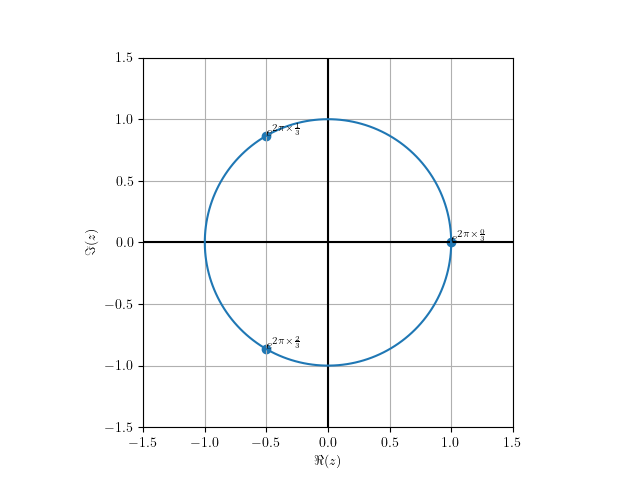
\includegraphics[scale=.33]{U_3.png}  
      \caption{$\U_3$}
      \label{fig:U3}
    \end{subfigure}
    \begin{subfigure}{.3\textwidth}
      \centering
      % include second image
      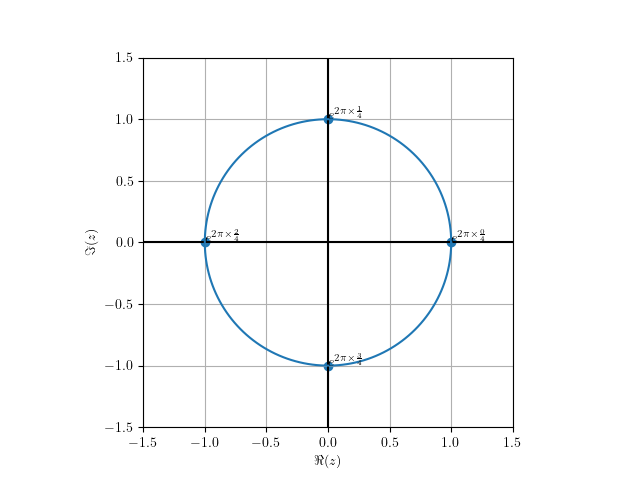
\includegraphics[scale=.33]{U_4.png}  
      \caption{$\U_4$}
      \label{fig:U4}      
    \end{subfigure}
    \begin{subfigure}{.3\textwidth}
      \centering
      % include second image
      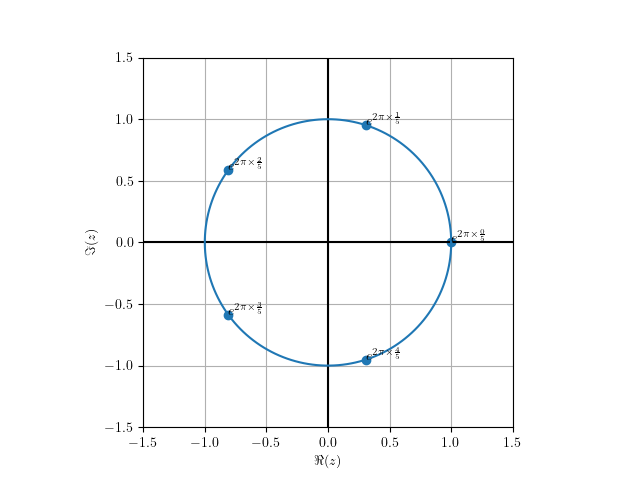
\includegraphics[scale=.33]{U_5.png}  
      \caption{$\U_5$}
      \label{fig:U5}      
    \end{subfigure}
    \newline
    \begin{subfigure}{.3\textwidth}
      \centering
      % include second image
      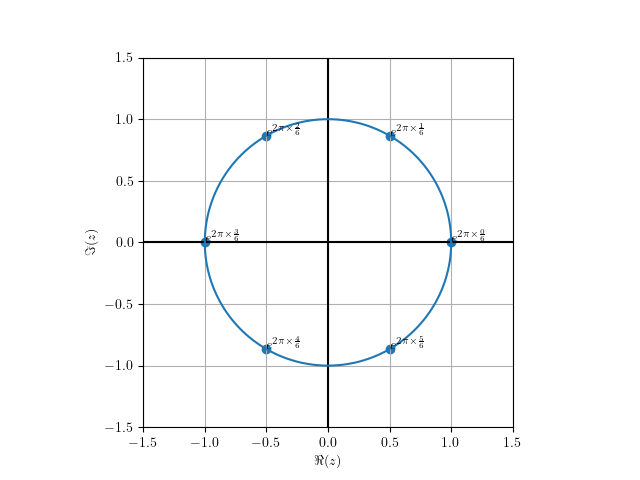
\includegraphics[scale=.33]{U_6.png}  
      \caption{$\U_6$}
      \label{fig:U6}      
    \end{subfigure}
    \begin{subfigure}{.3\textwidth}
      \centering
      % include first image
      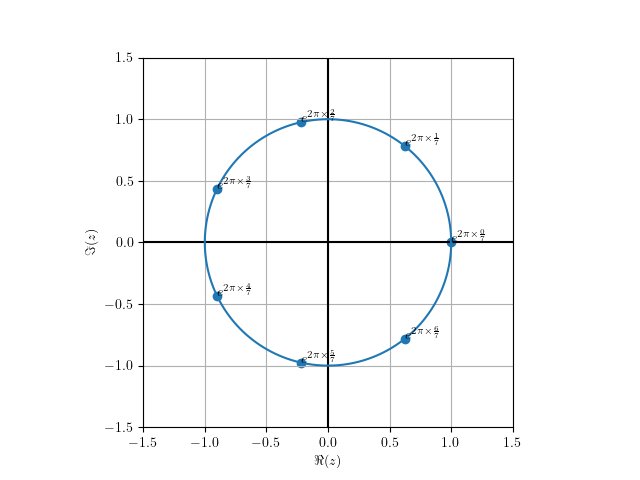
\includegraphics[scale=.33]{U_7.png}  
      \caption{$\U_7$}
      \label{fig:U7}
    \end{subfigure}
    \begin{subfigure}{.3\textwidth}
      \centering
      % include second image
      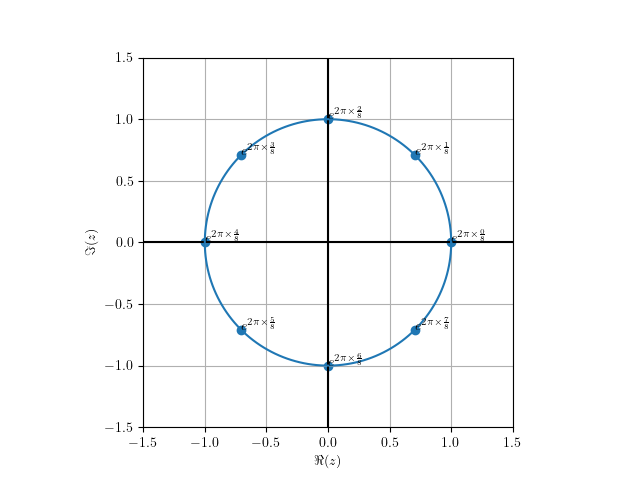
\includegraphics[scale=.33]{U_8.png}  
      \caption{$\U_8$}
      \label{fig:U8}      
    \end{subfigure}
    \newline
    \begin{subfigure}{.3\textwidth}
      \centering
      % include second image
      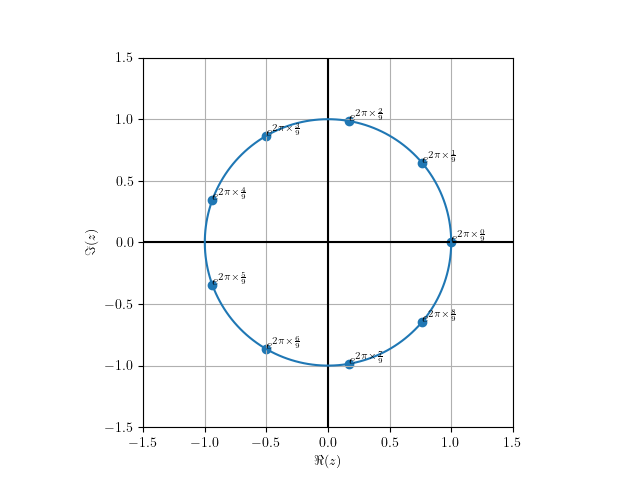
\includegraphics[scale=.33]{U_9.png}  
      \caption{$\U_9$}
      \label{fig:U9}      
    \end{subfigure}
    \begin{subfigure}{.3\textwidth}
      \centering
      % include second image
      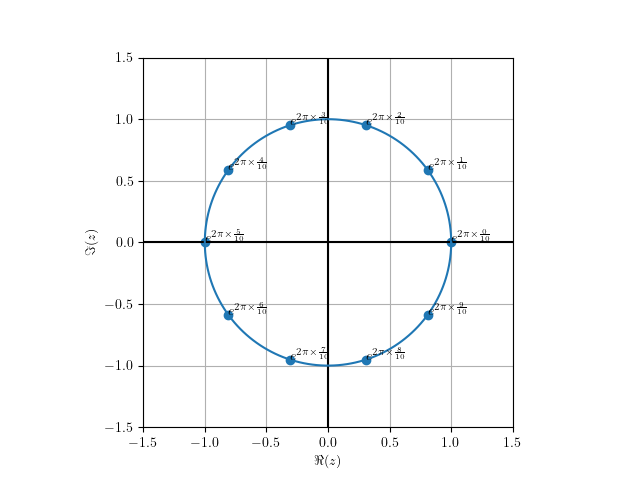
\includegraphics[scale=.33]{U_10.png}  
      \caption{$\U_{10}$}
      \label{fig:U10}
    \end{subfigure}  
    \begin{subfigure}{.3\textwidth}
      \centering
      % include first image
      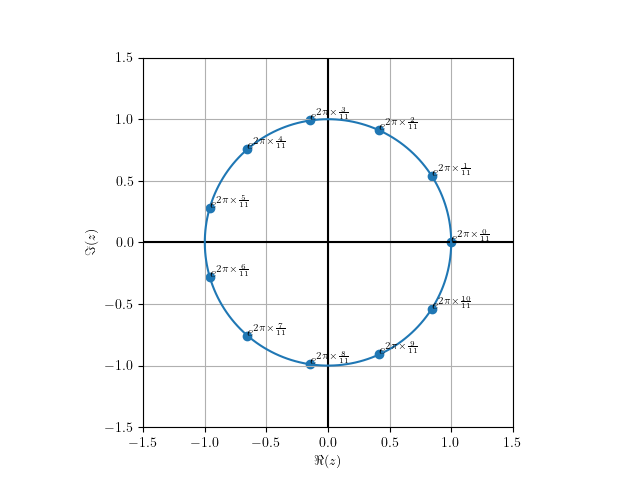
\includegraphics[scale=.33]{U_11.png}  
      \caption{$\U_{11}$}
      \label{fig:U11}
    \end{subfigure}
    \newline
    \begin{subfigure}{.3\textwidth}
      \centering
      % include second image
      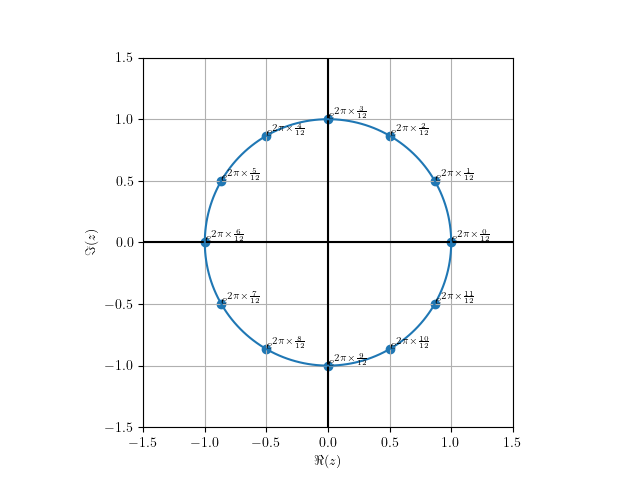
\includegraphics[scale=.33]{U_12.png}  
      \caption{$\U_{12}$}
      \label{fig:U12}      
    \end{subfigure}
    \begin{subfigure}{.3\textwidth}
      \centering
      % include second image
      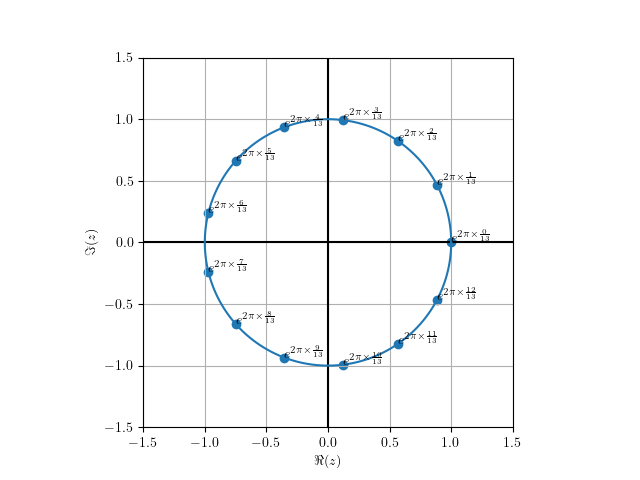
\includegraphics[scale=.33]{U_13.png}  
      \caption{$\U_{13}$}
      \label{fig:U13}      
    \end{subfigure}
    \begin{subfigure}{.3\textwidth}
      \centering
      % include second image
      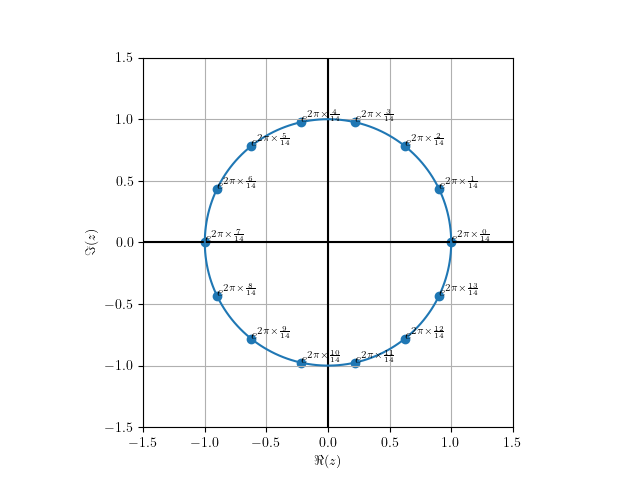
\includegraphics[scale=.33]{U_14.png}  
      \caption{$\U_{14}$}
      \label{fig:U14}
    \end{subfigure}
 \caption{Représentations graphique de $\U_3$, \ldots, $\U_{14}$}
  \label{fig:racinesnieme}
\end{figure}

\begin{theo}
  Soit \(n\) un entier naturel non nul alors
  \begin{equation}
    \forall z \in \U_n \setminus \{1\} \quad \sum_{k=0}^{n-1} z^k = 0.
  \end{equation}
\end{theo}
\begin{proof}
  C'est la somme des termes d'une suite géométrique de raison \(z \neq 1\) donc
  \begin{equation}
    \sum_{k=0}^{n-1} z^k = \frac{1-z^{n-1+1}}{1-z} = 0.
  \end{equation}
\end{proof}

Application à la résolution de \(z^n=a\) pour \(a \in \C\)~: On étudie ce problème en étude de cas~:
\begin{itemize}
\item si \(a=0\), la seule solution est zéro;
\item si \(a \neq 0\), on cherche des solutions dans \(\C^*\) et on peut écrire les formes trigonométriques~: \(z=\expc{\rho}{\theta} \quad a = \expc{A}{\alpha}\), alors
  \begin{equation}
    \rho = \sqrt[n]{A} \quad \congru{\theta}{\frac{\alpha}{n}}{\frac{2\pi}{n}};
  \end{equation}
  soit \(z_0=\expc{\sqrt[n]{A} }{\frac{\alpha}{n}}\), c'est une solution de l'équation; une solution \(z\) de l'équation est telle que \(\frac{z}{z_0} \in \U_n\)
\end{itemize}
%
\begin{prop}
  Pour un complexe \(a\) non nul, l'ensemble des solutions de l'équation \(z^n=a\) est
  \begin{equation}
    S_{z^n=a}=\enstq{\expc{\sqrt[n]{A}}{\frac{(\alpha + 2\pi k)}{n}}}{k \intervalleentier{0}{n-1}}.
  \end{equation}
  Si on connaît une solution \(z_0\) de l'équation, alors
  \begin{equation}
    S_{z^n=a}=\enstq{\expc{z_0}{\frac{2 k \pi}{n}}}{k \in \intervalleentier{0}{n-1}}.
  \end{equation}
\end{prop}
\emph{Cas particulier}
Si \(n=2\), on trouve deux racines complexes conjuguées. Par exemple les racines de \(Z=3+4\ii\) sont telles que
\begin{align}
  z^2=3+4\ii & \iff  \begin{cases} x^2-y^2=3 \\ 2xy=4 \end{cases} \\
  & \iff \begin{cases} x^2=4 \\ y^2=1 \\ xy=2 \end{cases} \\
  & \iff z \in \{2+\ii, -2-\ii\}.
\end{align}
%
\section{Résolution d'équations du second degré}
\label{sec:resolutionequationseconddegre}
\subsection{Résolution}
\label{subsec:resolution}
Soient \(a\), \(b\), \(c\) trois complexes avec a non nul. On s'intéresse à l'équation
\begin{equation}
  \label{eq:eq1}
  az^2+bz+c=0,
\end{equation}
avec \(z \in \C\) l'inconnue. On note \(\mathcal{S}\) l'ensemble des solutions de l'équation \eqref{eq:eq1}. Ces solutions sont les racines complexes du trinôme \(aX^2+bX+c\).

Mise sous forme canonique du trinôme~: le trinôme peut se factoriser en cherchant les racines
\begin{align}
  az^2+bz+c &= a \left(z^2+ 2 \frac{b}{2a}z + \frac{b^2}{4a^2} - \frac{b^2}{4a^2} +\frac{c}{a} \right)\\
  &=a \left( \left(z+\frac{b}{2a} \right)^2 - \frac{b^2-4ac}{4a^2} \right).
\end{align}
Comme \(a\) est non nul, les solution de l'équation \eqref{eq:eq1} sont des solutions de l'équation
\begin{equation}
  \left(z+\frac{b}{2a} \right)^2 - \frac{b^2-4ac}{4a^2} =0.
\end{equation}
%
\begin{defdef}
  On définit le discriminant de l'équation \eqref{eq:eq1} comme étant le complexe \(\Delta=b^2-4ac\).
\end{defdef}
%
\begin{enumerate}
\item Soit le discriminant est nul et auquel cas l'ensemble des solutions est
  \begin{equation}
    \mathcal{S}=\biggl\lbrace-\frac{b}{2a} \biggl\rbrace;
  \end{equation}
\item soit le discriminant est non nul et dans ce cas on pose que le complexe \(\delta\) est une de ses racines carrées et l'ensemble des solutions est
\begin{equation}
  \mathcal{S}=\biggl\lbrace \frac{-b+\delta}{2a} , \frac{-b-\delta}{2a} \biggl\rbrace.
\end{equation}
\end{enumerate}

\emph{Cas particulier} : si \(a\), \(b\) et \(c\) sont réels alors le discriminant \(\Delta\) de l'équation \eqref{eq:eq1} est réel et admet deux racines (si \(\Delta \neq 0\)) et donc~:
\begin{itemize}
\item soit le discriminant est positif et alors
  \begin{equation}
    \Delta >0 \quad \delta=\sqrt{\Delta} \quad \mathcal{S} = \biggl\lbrace \frac{-b+\sqrt{\Delta}}{2a} , \frac{-b-\sqrt{\Delta}}{2a} \biggl\rbrace;
  \end{equation}
\item soit le discriminant est négatif et alors
  \begin{equation}
    \Delta <0 \quad \delta=\ii\sqrt{\Delta} \quad \mathcal{S} = \biggl\lbrace \frac{-b+\ii\sqrt{-\Delta}}{2a} , \frac{-b-\ii\sqrt{-\Delta}}{2a} \biggl\rbrace.
  \end{equation}
\end{itemize}
Si le nombre \(2\) apparaît naturellement en facteur dans \(b\), on pose \(b'=\frac{b}{2}\) et on définit le discriminant réduit~: \(\Delta'=b'^2-ac\) et les solutions sont sous la forme \(\frac{-b'\pm \delta'}{a}\).
%
\begin{theo}[Théorème fondamental de l'algèbre (1799 -- Gauss)]
  Toute équation polynomiale de degré \(n\) admet \(n\) solutions dans \(\C\).
\end{theo}
\begin{proof}
  La preuve n'est pas au programme de MPSI.
\end{proof}
%
\subsection{Relation entre les coefficients et les racines}
\label{subsec:relationcoefsracines}
%
\begin{prop}
  Soient \(s\) et \(p\) deux complexes. Alors deux complexes quelconques \(x\) et \(y\) sont solutions de \(\begin{cases} x +y = s \\ xy=p \end{cases}\) si et seulement si \(x\) et \(y\) sont solutions de l'équation \(z^2 -sz+p=0\).
\end{prop}
\begin{proof}
  Soient \(s\) et \(p\) deux complexes. On considère l'équation
  \begin{equation}
    z^2-sz+p=0.
  \end{equation}
  Soient \(\alpha\) et \(\beta\) les solutions de cette équation, alors
  $\begin{cases} \
    \alpha +\beta = s \\
    \alpha \beta=p
  \end{cases}$.
  Plus généralement si \(\alpha\) et \(\beta\) sont les deux racines de l'équation \eqref{eq:eq1} alors \(\begin{cases} \alpha + \beta = -\frac{b}{a} \\ \alpha \beta = \frac{c}{a} \end{cases}\).
\end{proof}
%
\section{Exponentielle complexe}
\label{sec:expcomplexe}
\begin{defdef}
  Soit \(z\) un nombre complexe. On définit l'exponentielle complexe de \(z\) (notée \(\exp(z)\) ou \(\e^z\)) par \(\exp(z)=\e^{\Re(z)}(\cos \Im(z) + \ii \sin \Im(z))\).
\end{defdef}
\begin{prop}
  L'application \(\fonction{}{\C}{\C^*}{z}{\e^z}\) est un morphisme du groupe \((\C,+)\) sur le groupe \((\C^*,\times)\)~\footnote{cf.\ chapitre~\ref{chap:groupes}}.
\end{prop}
\begin{proof}
  Si on note avec quatre réels \(x,x',y,y'\) les complexes \(z=x+\ii y\) et \(z'=x'+\ii y'\) alors
  \begin{align}
    \e^{z+z'} =& \e^{(x+x') + \ii(y+y')}\\
    =&\e^{x+x'} \e^{\ii (y+y')}\\
    =& \e^{x} \e^{x'} \e^{\ii y} \e^{\ii y'}\\
    =& \e^z \e^{z'}.
  \end{align}
\end{proof}
%
\begin{prop}
  Soient \(z\) et \(z'\) deux complexes alors
  \begin{equation}
    \e^z=\e^{z'} \iff \congru{z}{z'}{2\pi \ii}.
  \end{equation}
\end{prop}
\begin{proof}
   Cette formule est due au caractère \(2\pi\)-périodique des fonctions sinus et cosinus.
 \end{proof}
%
 \begin{prop}
   Soit un intervalle \(I\) réel et \(\varphi \in \C^{I}\) une application dérivable. Alors \(f=\e^\varphi\) est dérivable telle que \(f'=\varphi' \e^\varphi\). En particulier si \(a\) est complexe, l'application \(\fonction{f_a}{\R}{\C}{x}{\e^{ax}}\) est dérivable sur \(\R\) et \(f_a'=af_a\).
 \end{prop}
 \begin{proof}
   Soient \(\varphi_1\) et \(\varphi_2\), respectivement la partie réelle de \(\varphi\) et la partie imaginaire de \(\varphi\). Alors
   \begin{align}
     \forall x \in I \quad f(x)=e^{\varphi(x)}&=\cos \varphi_2(x) \e^{\varphi_1(x)}+ \ii \sin \varphi_2(x)\e^{\varphi_1(x)} \\
     &= \Re[f(x)] + \Im[f(x)].
   \end{align}
  Comme \(\varphi\) est dérivable, \(\varphi_1=\Re[f]\) et \(\varphi_2=\Im[f]\) le sont, ainsi \(f\) est dérivable.
\end{proof}
\emph{Remarque}~: L'application \(\fonction{f}{\C}{\C}{z}{\e^z}\) n'est pas dérivable.
\section{Nombres complexes et géométrie plane}
\label{sec:complexesetgeometrie}
\subsection{Écriture complexe de quelques transformations usuelles du plan}
\label{subsec:ecriturecomplexeettransformations}
À toute transformation \(F\) du plan \(\P\), on peut associer un application \(f \in \C^{\C}\) telle que pour tous points \(M(z)\) et \(M'(z')\) on ait
\begin{equation}
  M'=f(M) \iff z'=f(z).
\end{equation}
On dit que \(F\) est représentée par l'application \(f\). Soient deux complexes \(z_0\) et \(b\) deux complexes correspondant respectivement à un point \(M_0\) et un vecteur \(\vect{u}\) du plan \(\P\).
\begin{itemize}
\item La rotation de centre \(M_0\) d'angle \(\theta\) est représentée par
  \begin{equation}
    \fonction{f}{\C}{\C}{z}{\expc{}{\theta}(z-z_0) +z_0};
  \end{equation}
\item la translation de vecteur \(\vect{u}\) est représentée par
  \begin{equation}
    \fonction{f}{\C}{\C}{z}{z+b};
  \end{equation}
\item la symétrie de centre \(M_0\) est représentée par
  \begin{equation}
    \fonction{f}{\C}{\C}{z}{2z_0-z};
  \end{equation}
\item l'homothétie de rapport \(k\neq 0\) et de centre \(M_0\) est représentée par
  \begin{equation}
    \fonction{f}{\C}{\C}{z}{k(z-z_0)+z_0}.
  \end{equation}
\end{itemize}
%
\subsection{Similitudes directes}
\label{subsec:simdirecte}
Soient \(\omega \in \C\), \(k\in \R^*\) et \(\theta \in \R^*\). La rotation \(\mathcal{R}\) de centre \(\omega\) et d'angle \(\theta\) est représentée par \[\fonction{r}{\C}{\C}{z}{\expc{}{\theta}(z-\omega)+\omega},\] et l'homothétie \(\mathcal{H}\) de rapport \(k \in \R^*\) est représentée par \[\fonction{h}{\C}{\C}{z}{k(z-\omega)+\omega}.\]
%
\begin{defdef}
  On appelle similitude directe de centre \(\Omega(\omega)\), d'angle \(\theta\) et de rapport \(k \in \R^*\), la transformation \(\Psi\) du plan dans le plan représentée par l'application \(\fonction{\psi}{\C}{\C}{z}{\expc{k}{\theta}(z-\omega)+\omega}\).
\end{defdef}

%
Soient \(a\) non nul et \(b\) dans \(\C\), on considère la bijection \(\fonction{\varphi}{\C}{\C}{z}{az+b}\) qui représente \(\fonction{\Phi}{\P}{\P}{M(z)}{M(az+b)}\).
\begin{itemize}
\item Si \(a=1\); alors  \(\Phi\) est la translation de vecteur \(\vect{u}(b)\).
\item Si \(a \neq 1\), alors on montre que \(\Phi\) admet un unique point fixe \(\Omega(\omega) \quad \omega = \frac{b}{1-a}\) et \(\varphi(z)=a(z-\omega)+\omega\).
  \(\Phi\) est la similitude de centre \(\Omega(\omega)\), de rapport \(k=\abs{a}\) et d'angle \(\congru{\theta}{\arg(a)}{2\pi}\)
\end{itemize}
%
\subsection{Application inversion}
\label{subsec:appinverse}
Soit l'application \(\fonction{f}{\C^*}{\C^*}{z}{\frac{1}{z}}\) la transformation du plan associée \(\fonction{F}{\P \setminus\{O\}}{\P \setminus\{O\}}{M(z)}{M \left( \frac{1}{z} \right)}\) est une inversion. Si \(M\) appartient au cercle trigonométrique, \(F(M)\) est le symétrique de \(M\) par rapport à l'axe des réels et il est sur le cercle.
%
\subsection{Barycentre}
\label{subsec:complexebarycentre}
Soient \(n \in \N^{*} \ , \ (A_1, \ldots A_n) \in \P^n\)  d'affixes respectives \(z_1 \ldots z_n\) et \(\lambda_1 \ldots \lambda_n\) des réels tels que \(\sum_{k=0}^{n} \lambda_k \neq 0\). Soit \(G\) le barycentre de ces points,n l'affixe de \(G\) est \(z_G=\frac{\sum_{k=1}^{n}\lambda_k z_k}{\sum_{k=1}^{n}\lambda_k}\)
%
\subsection{Orthogonalité}
\label{subsec:complexeorthogonalite}
Soient \(\vect{v}\) et \(\vect{v'}\) deux vecteurs d'affixes respectives \(z=x+\ii y\) et \(z'=x'+\ii y'\). On sait que \(\vect{v}\) et \(\vect{v'}\) sont orthogonaux si et seulement si leur produit scalaire est nul. Soit \(\vect{v}\) et \(\vect{v'}\) si et seulement si \(\Re(z \bar{z'})=0\).
%
\subsection{Alignement}
\label{subsec:complexealignement}
Soient deux réels \(k\) et \(\lambda\).
\begin{enumerate}
\item Quel est l'ensemble des points \(E_k = \enstq{M(z) \in \P}{\abs{\frac{z-a}{z-b}}=k}\)~?
\item Quel est l'ensemble des points \(E_\lambda = \enstq{M(z) \in \P}{\congru{\arg \left(\frac{z-a}{z-b} \right)}{\lambda}{2\pi}}\)~?
\end{enumerate}

Si le réel \(k<0\) alors \(E_k=\emptyset\), s'il est nul alors \(E_0=\{A(a)\}\), s'il vaut 1 alors \(E_1\) est la médiatrice de \([AB]\).

Si le réel \(k\) est strictement positif non égal à 1 alors \(\frac{MA}{MB}=k\) et donc \((\vect{MA}+k\vect{MB}) \cdot (\vect{MA}-k\vect{MB})=0\). Soit \(I\) le barycentre de \((A,1)(B,k)\) et \(J\) le barycentre de \((A,1)(B,-k)\) alors \((1+k)(1-k) \vect{MI} \cdot \vect{MJ} =0\) comme \(k \neq \pm 1\) on a que M est sur le cercle de diamètre \([IJ]\).

Si \(z \in \{a,b\}\) alors \(E_\lambda=\emptyset\) et sinon \(E_\lambda\) est la droite qui forme l'angle \(\lambda\) avec la droite \((A(a)B(b))\).
\cleardoublepage
\section{Exercices}
\begin{exercice}[Identité du parallèlogramme]
    Démontrer que pour tous nombres complexes \(z\) et \(z'\) on a~:\(\abs{z+z'}^2 + \abs{z-z'}^2 = 2\abs{z}^2 + 2\abs{z'}^2\).
\end{exercice}
\begin{exercice}
    Soient un naturel \(n\) et un réel \(a\) tel que \(0 \leqslant a < 2\pi\). Calculer le module et l'argument (s'il existe) de \(z = (1+\ii\e^{\ii a})^n\)
\end{exercice}
\begin{exercice}
    Mettre les nombres complexes suivants sous forme algébrique~: \(\alpha = \frac{9-4\ii}{3+2\ii}\), \(\beta=(1-\ii\sqrt{3})^{2007}\), \(\gamma = \frac{(1+j)^3+(1-j)^3}{(1+j)(1+j^2)}\) et \( \delta = \e^{1+i}\).
\end{exercice}
\begin{exercice}
    Soient \(a\) et \(b\) des réels de \(\intervallefo{0}{2\pi}\). On pose \(u=\e^{a\ii}\) et \(v=\e^{b\ii}\). Déterminer le module et un argument, si possible, de chacun des complexes~: \(1+u\) et \(\frac{u+v}{1+uv}\).
\end{exercice}
\begin{exercice}[Théorème de l'angle inscrit]
    Soient \((a, b, c) \in \C^3\) tels que \(\abs{a}=\abs{b}=\abs{c}=1\) et \(a \neq c\) et \(b \neq c\). Montrer que~:\(\Arg \frac{c-b}{c-a} \equiv \frac{1}{2} \Arg \frac{b}{a} \pmod \pi\). En donner une interprétation géométrique.
\end{exercice}
\begin{exercice}
    Résoudre sur \(\C\), de deux façons, l'équation \(z^4+z^3+z^2+z+1=0\). L'une des deux méthodes consistera à se ramener à une équation du deuxième degré obtenue en faisant le changement de variable \(y = z+1/z\). Déterminer des expressions de \(\cos 2\pi/5\) et \(\sin 2\pi/5\).
\end{exercice}
\begin{exercice}
    Soient \(A\), \(B\), et \(C\) trois points non alignés du plan complexe d'affixes respectives \(a\), \(b\) et \(c\). Montrer l'équivalence entre les trois propriétés suivantes~:
    \begin{enumerate}
        \item Le triangle \(ABC\) est équilatéral;
        \item \(a+bj+cj^2=0\) ou \(a+bj^2+cj=0\);
        \item \(a^2+b^2+c^2=ab+ac+bc\).
    \end{enumerate}
\end{exercice}
\begin{exercice}
    Déterminez les nombres complexes \(z\) tels que \(z, 1/z\) et \(z-1\) aient le même module.
\end{exercice}
\begin{exercice}
    On pose \(a=\e^{2\ii\pi/7}\). Déterminer une expression de chacun des complexes \(A = a+a^2+a^4 \qquad B = a^3+a^5+a^6\).
\end{exercice}
\begin{exercice}
    Soient \(n \in \N^{*}\) et \((z_1, \ldots, z_n) \in (\C^{*})^n\).
    \begin{enumerate}
        \item Montrer que \( \abs{\sum_{k=1}^n z_k} \leqslant \sum_{k=1}^n \abs{z_k}\).
        \item Montrer qu'il y a égalité dans cette inégalité si et seulement si~: \(\Arg(z_1) \equiv \Arg(z_2) \equiv \cdots \equiv \arg(z_n) \pmod{2\pi}\)
        \item Montrer qu'il y a égalité dans cette inégalité si et seulement si, pour tout couple \((a,b) \in \intervalleentier{1}{n}^2 \ z_a \bar{z_b} \in \Rpluss\).
    \end{enumerate}
\end{exercice}
\begin{exercice}
    Soient un réel \(\alpha\) et un naturel non nul \(n\) fixés. Résoudre dans \(\C\) les équations suivantes~:
    \begin{multicols}{2}
        \begin{enumerate}
            \item \(z^2 = 46-14\ii\sqrt{3}\)
            \item \(z^2-2\cos(\alpha)z+1=0\)
            \item \(z+\bar{z}=\abs{z}\)
            \item \((1+\ii)z^2+3(1-\ii)z-2(2+\ii)=0\)
            \item \(z^4-(3+i)z^2+4+3\ii=0\)
            \item \(z^{2n}+z^n+1=0\)
            \item \(\left(1+\frac{\ii z}{n}\right)^n = \left(1-\frac{\ii z}{n}\right)^n\)
        \end{enumerate}
    \end{multicols}
\end{exercice}
\begin{exercice}
    Déterminer l'ensemble des points \(M\) du plan complexe d'affixe \(z\) tels que~:
    \begin{enumerate}
        \item le nombre \(\frac{z+2}{z+3\ii}\) soit réel
        \item Le nombre \(\left(\frac{z+1}{z-1}\right)^2\) soit imaginaire pur
        \item \(\abs{\frac{z-1}{z+1}}=2\).
    \end{enumerate}
\end{exercice}
\begin{exercice}
    Soient \(a\) et \(h\) deux nombre réels et \(n\) un naturel non nul. Donner une expression simple des sommes suivantes~: \( C_n = \sum_{k=0}^{n-1} \cos(a+kh), S_n = \sum_{k=0}^{n-1} \sin(a+kh)\)
\end{exercice}
\begin{exercice}
    Soient \(a\) un réel et \(n\) un naturel non nul. Donner une expression simple de la somme~: \(T_n = \sum_{p=1}^n \cos^p a \sin(pa)\).
\end{exercice}
\begin{exercice}
    Soient \(n \in \N\setminus\{0,1\}\) et \(\omega = \e^{2\ii\pi/n}\), \(a\) et \(b\) deux complexes. Montrer que~:
\(\abs{a+b} \leqslant \frac{2}{n} \sum_{k=0}^{n-1} \abs{a+\omega^k b}\).
\end{exercice}
\begin{exercice}
    Résoudre dans \(\C\) les systèmes suivants
    \begin{equation}
        (1) \begin{cases} x+y+z=1 \\ xyz=1 \\ \abs{x}=\abs{y}=\abs{z}=1 \end{cases}
        (2) \begin{cases} 5x-\ii{}y=2 \\ (1+\ii)x+3y=5 \end{cases}
        (3) \begin{cases} (1+\ii)x+\bar{y} = 3+7\ii \\\bar{x}+y=2+\ii\end{cases}
    \end{equation}
\end{exercice}
\begin{exercice}
    Déterminer toutes les applications \(f \in \C^{\C}\) telles que \(\forall z \in \C, f(z)+\ii f(\bar{z}) = 1+z\)
\end{exercice}
\begin{exercice}[Méthode de Cardan]
    Soient \(a, b, c\) des réels. On considère l'équation du troisième degré
    \begin{equation}
        X^3+aX^2+bX+c=0
    \end{equation}
    \begin{enumerate}
        \item à l'aide du changement de variable \(Y = X+a/3\), montrer qu'on peut se ramener à la résolution d'une équation de la forme~:
            \begin{equation}
                \label{eq:cardan1}
                Y^3+pY+q = 0,
            \end{equation}
            avec \(p\) et \(q\) deux réels.
        \item Soit \(y\) une racine de l'équation~\eqref{eq:cardan1}. Montrer qu'il existe un couple \((u,v)\) de complexes tel que \(u+v=y\) et \(uv=-p/3\), et que \(u^3\) et \(v^3\) sont racines de l'équation~\eqref{eq:cardan2}
            \begin{equation}
                \label{eq:cardan2}
                Z^2+qZ-p^3/27 = 0.
            \end{equation}
         \item Résoudre l'équation~\eqref{eq:cardan2} en discutant selon la valeur de \(\Delta_3 = 4p^3+27q^2\).
         \item En déduire les racine de l'équation~\eqref{eq:cardan1}. En particulier, on discutera le nombre de racines réelles.
    \end{enumerate}
\end{exercice}

\chapter{Théorie des ensembles et des applications}
\label{chap:ensembles}
\minitoc
\minilof
\minilot

La théorie des ensembles comprend l'étude des ensembles, l'étude de leurs parties et l'étude de leurs interactions grâce aux applications. On s'intéresse particulièrement aux injections, aux surjections et aux bijections. La troisième section présente les relations binaires comme la relation d'ordre ou la relation d'équivalence. La quatrième et dernière section se focalise sur les familles d'éléments comme par exemple des suites. 

Ce chapitre est primordial dans le programme de MPSI, il décrit le langage nécessaire pour travailler de manière sérieuse en mathématiques.
%
\section{Vocabulaire relatif aux ensembles}
\label{chap3-sec:vocabensemble}
Nous prenons comme notion primitive les notions d'ensemble, d'élément et d'appartenance. On ne cherchera pas à les définir, \og\(x \in E\)\fg{} sera lu \og \emph{l'élément \(x\) appartient à l'ensemble \(E\)} \fg{}.
%
\subsection{Égalité de deux ensembles}
\label{chap3-subsec:egalitededeuxensembles}
\begin{defdef}
  On dira que deux ensembles \(E\) et \(F\) sont égaux si ils ont les mêmes éléments. On notera \(E=F\),
  \begin{equation}
    E=F \iff \forall x \quad \left(x \in E \iff x \in F \right).
  \end{equation}
\end{defdef}
%
\subsection{Inclusion}
\label{chap3-subsec:inclusion}
\begin{defdef}
  Soient \(E\) et \(F\) deux ensembles. On dira que \(E\) est inclus dans \(F\) ou que \(E\) est un sous-ensemble de \(F\) si et seulement si tous les éléments de \(E\) sont des éléments de F. On notera \(E \subset F\)
\end{defdef}
\begin{prop} 
  \begin{equation}
    E=F \iff E \subset F \textrm{~et~} F \subset E.
  \end{equation}
\end{prop}
Pour dire que \(E\) est strictement inclus dans \(F\) c'est à dire \(E \subset F \textrm{~et~} F \not\subset E\), on notera \(E \subsetneq F\)
\begin{equation}
  E \subsetneq F \iff \left[\forall x \quad \left(x \in E \iff x \in F \right) \right] \textrm{~et~} \left[\exists x \in F \quad x \not\in E \right].
\end{equation}
%
\subsection{Ensemble des parties d'un ensemble}
\label{chap3-subsec:ensembledesparties}
\begin{axiome}[Axiome de l'ensemble des parties]
  Soit un ensemble \(E\). Il existe un ensemble dont les éléments sont les parties de \(E\). On l'appelle ensemble des partie de \(E\) et il est noté \(\Part(E)\) et
\begin{equation}
  A \in \Part(E) \iff A \subset E.
\end{equation}
\end{axiome}
Il n'y a que deux autres façons de définir un ensemble~:
\begin{itemize}
\item en extension, c'est-à-dire qu'on énumère les éléments de l'ensemble, par exemple \(S=\{1;2;3\}\) ;
\item en compréhension, c'est-à-dire qu'on définit l'ensemble \(E\) comme sous-ensemble d'un ensemble plus grand. Le sous ensemble des éléments de \(F\) qui vérifie une certaine propriété, par exemple l'ensemble des entiers pairs de \(\Z\), \(E_1=\enstq{n\in\Z}{\exists k \in \Z \quad n=2k}\).
\end{itemize}
%
\subsection{Opérations sur les parties d'un ensemble}
\label{chap3-subsec:operationparties}
Soient \(E\) un ensemble, \(A\) et \(B\) des parties de \(E\). On définit les opérations sur les ensembles \(A\) et \(B\) suivantes
décrites dans les paragraphes suivants.
%
\subsubsection{Complémentaire de \(A\) dans \(E\)} 
\label{chap3-subsubsec:complementaire}
C'est l'ensemble de \(E\) qui ne sont pas des éléments de \(A\), noté \(\complement_E A\) ou \(\bar{A}\)~\footnote{ne pas confondre avec l'adhérence, cf programme de MP} ou \(E \setminus A\).
\begin{equation} 
  \forall x \in E \quad x \in \complement_E A \iff x \not\in A.
\end{equation}
Le diagramme de Venn correspondant est donné par la figure~\ref{chap3-fig:comp}.
%
\begin{figure}
\centering
\begin{tikzpicture}
\draw \En; 
\fill[pink] \An; 
%\fill[green, opacity=0.2] \Bn;
\draw (-4,-1) node[above right]{\(E\)}; 
\draw (-2,0) node{\(A\)}; 
\draw (0,-0.5) node{\(\bar{A}\)}; 
%\draw (2,0) node{\(B\)};
\end{tikzpicture}
\caption{Représentation du complémentaire}
\label{chap3-fig:comp}
\end{figure}
%
\begin{prop}
  Soient \(A\) et \(B\) deux parties de \(E\)
  \begin{gather}
  \complement_E (\complement_E A)=A; \label{eq:comp1}\\
  A \subset B \iff \complement_E B \subset \complement_E A. \label{eq:comp2}
  \end{gather}
\end{prop}
\begin{proof}
    Prouvons \eqref{eq:comp1}. Soit \(a \in E\), \(a \in \complement_E (\complement_E A)\) équivaut à \(a \not\in \complement_E A\) ; ce qui équivaut à \(a \in A\). Prouvons la première implication de \eqref{eq:comp2}. Soit \(x \in \complement_E B\) alors \(x \not\in B\), alors par hypothèse, \(A \subset B\), \(x\) ne peut pas être dans \(A\), \(x \not\in A\), donc \(x\) est dans le complémentaire de \(A\)~: \(x \in \complement_E A\).

    Prouvons la deuxième implication de \eqref{eq:comp2}. Soit \(x \in A\), alors \(x \not\in \complement_E A\), alors par hypothèse, \(\complement_E B \subset \complement_E A\), \(x\) ne peut pas être dans \(\complement_E B\), \(x \not\in \complement_E B\), donc par définition du complémentaire, \(x \in B\).
\end{proof}
%
\subsubsection{Intersection des parties \(A\) et \(B\)}
\label{chap3-subsubsec:intersection}
C'est l'ensemble des éléments qui sont à la fois dans \(A\) et dans \(B\), on le note \(A \cap B\),
\begin{equation}
  \forall x \in E \quad x \in A \cap B \iff x \in A \text{~et~} x \in B.
\end{equation}
Le diagramme de Venn correspondant est donné par la figure~\ref{chap3-fig:inter}.

\begin{figure}
\centering
\begin{tikzpicture}
\draw \En; 
\fill[red, opacity=0.2] \An; 
\fill[green, opacity=0.2] \Bn;
\fill[blue, opacity=0.5] \AnB;
\draw (-4,-1) node[above right]{\(E\)}; 
\draw (-2,0) node{\(A\)}; 
\draw (2,0) node{\(B\)};
\draw (0,2) node{\(A \cap B\)};
\end{tikzpicture}
\caption{Représentation de l'intersection}
\label{chap3-fig:inter}
\end{figure}

\subsubsection{Réunion des parties \(A\) et \(B\)}
\label{chap3-subsubsec:reunion}
C'est l'ensemble des éléments qui appartiennent au moins à l'une des parties \(A\) et \(B\), on le note \(A \cup B\).
\begin{equation}
  \forall x \in E \quad x \in A \cup B \iff x \in A \text{~ou~} x \in B
\end{equation}
Le diagramme de Venn correspondant est donné par la figure~\ref{chap3-fig:reunion}.

\begin{figure}
\centering
\begin{tikzpicture}
\draw \En; 
\fill[red, opacity=0.2] \An; 
\fill[green, opacity=0.2] \Bn;
\fill[blue, opacity=0.5] \AuB;
\draw (-4,-1) node[above right]{\(E\)}; 
\draw (-2,0) node{\(A\)}; 
\draw (2,0) node{\(B\)};
\draw (0,2) node{\(A \cup B\)};
\end{tikzpicture}
\caption{Représentation de la réunion}
\label{chap3-fig:reunion}
\end{figure}

\subsubsection{Différence de A et B}
\label{chap3-subsubsec:difference}
C'est l'ensemble des éléments de \(E\) qui appartiennent à \(A\) mais pas à \(B\), noté \(A \setminus B\).
\begin{gather}
  \forall x \in E \quad x \in A \setminus B \iff x \in A \text{~et~} x \not\in B; \\
  A \setminus B=A \cap \complement_E B.
\end{gather}
Le diagramme de Venn correspondant est donné par la figure~\ref{chap3-fig:diff}.

\begin{figure}
\centering
\begin{tikzpicture}
\draw \En; 
\fill[red, opacity=0.2] \An; 
\fill[green, opacity=0.2] \Bn;
\fill[blue, opacity=0.5] \AmB;
\draw (-4,-1) node[above right]{\(E\)}; 
%\draw (-2,0) node{\(A\)}; 
\draw (2,0) node{\(B\)};
\draw (-2,2) node{\(A \setminus B\)};
\end{tikzpicture}
\caption{Représentation de la différence \(A \setminus B\)}
\label{chap3-fig:diff}
\end{figure}

\subsubsection{Différence symétrique de \(A\) et \(B\)}
\label{chap3-subsubsec:differencesymetrique}
C'est l'ensemble des éléments de \(E\) qui appartiennent à exactement une des parties \(A\) et \(B\), on le note $A \Delta
B$~:
\begin{equation}
  \forall x \in E \quad x \in A \Delta B \iff x \in A \cup B \text{~et~} x \not\in A \cap B.
\end{equation}
Le diagramme de Venn correspondant est donné par la figure~\ref{chap3-fig:diffsym}.

\begin{figure}
\centering
\begin{tikzpicture}
\draw \En; 
\fill[red, opacity=0.2] \An; 
\fill[green, opacity=0.2] \Bn;
\fill[blue, opacity=0.5] \AmB;
\fill[blue, opacity=0.5] \BmA;
\draw (-4,-1) node[above right]{\(E\)}; 
%\draw (-2,0) node{\(A\)}; 
%\draw (2,0) node{\(B\)};
\draw (-1,2) node{\(A \Delta B\)};
\end{tikzpicture}
\caption{Représentation de la différence symétrique \(A \Delta B\)}
\label{chap3-fig:diffsym}
\end{figure}

\begin{prop}
  Soient \(A\) et \(B\) des parties de \(E\), on a 
  \begin{gather}
    A \Delta B = (A\setminus B) \cup (B \setminus A) = (A \cap \bar{B}) \cup (B \cap \bar{A}); \\
    A \Delta B =(A \cup B) \setminus (B \cap A) = (A \cup B) \cap \bar{A \cap B} =(A \cup B) \cap (\bar{A} \cup \bar{B})
  \end{gather}
\end{prop}

\subsubsection{Propriétés}
\label{chap3-subsubsec:prop}
\begin{axiome}
  Soient \(A, B\) et \(C\) trois parties de \(E\), on a les axiomes suivants respectivement~:
  \begin{itemize}
    \item La commutativité
        \begin{gather}
            A \cap B= B \cap A, \\  
            A \cup B=B \cup A;
        \end{gather}
    \item l'associativité
        \begin{gather}
            A \cap (B \cap C)=(A \cap B) \cap C, \\ 
            A \cup (B \cup C)=(A \cup B) \cup C;
        \end{gather}
    \item la distributivité
        \begin{gather}
            A \cap (B \cup C)=(A \cap B) \cup (B \cap C), \\ 
            A \cup (B \cap C)=(A \cup B) \cap (A \cup C);
        \end{gather}
    \item la stabilité
        \begin{gather}
            A \subset B \implies (A \cap C) \subset (B \cap C), \\ 
            A \subset B \implies (A \cup C) \subset (B \cup C);
        \end{gather}
    \item les lois de De Morgan
        \begin{gather}
            \complement_E (A \cup B)=\complement_E A \cap \complement_E B, \\ 
            \complement_E (A \cap B)=\complement_E A \cup \complement_E B;
        \end{gather}
    \item les lois de Boole
        \begin{gather}
            A \cap (A \cup B)=A, \\ 
            A \cup (A \cap B)=A.
        \end{gather}
    \end{itemize}
\end{axiome}
%
\subsection{Ensemble vide}
\label{chap3-subsec:ensemblevide}
Si \(E\) est un ensemble, \(\complement_E E\) est la seule partie de \(E\) sans élément. On l'appelle la partie vide de \(E\). Si \(F\) est un autre ensemble, on a \(\complement_E E = \complement_F F\). On parlera de l'ensemble vide de \(E\) au lieu de dire la partie vide de \(E\), on le note \(\emptyset\). Quelque soit l'ensemble \(E\), \(\complement_E E =\emptyset\).

Faire attention à ne pas confondre \(\emptyset = \{\}\) qui ne contient rien avec \(\{\emptyset\}\) qui contient l'ensemble
vide.

\subsection{Produit cartésien de deux ensembles}
\label{chap3-subsec:prodcart}
\begin{defdef}
  Pour deux éléments \(x\) et \(y\) de \(E\), on appelle couple \((x,y)\) la partie \(\{\{x\},\{x;y\}\}\). C'est un artifice pour se donner les éléments dans un certain ordre.
\end{defdef}
%
\begin{prop}
  Soient quatre éléments de \(E\), \(x\) ,\(y\), \(x'\) et \(y'\) alors 
  \begin{equation} 
    (x,y)=(x',y') \iff \begin{cases} x=x' \\ y=y' \end{cases}.
  \end{equation}
\end{prop}
\begin{proof}
Supposons que \(x=x'\) et \(y=y'\), alors 
\begin{equation}
  (x,y)=\{\{x\},\{x,y\}\}=\{\{x'\},\{x',y'\}\}=(x',y').
\end{equation}
Si on suppose maintenant que \((x,y)=(x',y')\) alors 
\begin{equation}
  \{\{x\},\{x,y\}\}=\{\{x'\},\{x',y'\}\}.
\end{equation}
Par l'absurde, si \(x \neq x'\) on a \(\{x\}=\{x',y'\}\) et \(\{x,y\} = \{x'\}\) donc \(x'=y'=x\) et \(y=x'=x\) donc on aboutit à la contradiction \(x=x'\). Nécessairement \(x'=x\) et donc \(y=y'\).
\end{proof}
%
\begin{defdef}
  Soient \(E\) et \(F\) deux ensembles, on appelle produit cartésien de \(E\) et \(F\), qu'on note \(E \times F\) l'ensemble $E
  \times F = \enstq{(x,y)}{x \in E \ y \in F}$.
\end{defdef}
Si \(E=F\) alors on note \(E \times E=E^2\). Si on dispose de \(n\) ensemble \(E_k\), on définit par récurrence le produit \(\prod_{k=1}^n E_k\) et les n-uplets \((x_k)\).

\section{Application}
\label{chap3-sec:applications}
\subsection{Notion d'application}
\label{chap3-subsec:notiondapplication}
\begin{defdef}
  On appelle application tout triplet \((E, F, \Gamma)\) où \(E\) et \(F\) sont des ensembles, \(\Gamma\) une partie de \(E \times F\) telle que 
  \begin{equation}
    \forall x \in E \ \exists! y \in F \quad (x,y) \in \Gamma.
  \end{equation}
\end{defdef}
Une représentation graphique de la notion d'application est donné sur la figure~\ref{chap3-fig:application}. Soit une
application \(f=(E,F,\Gamma)\), alors \(E\) est l'ensemble de départ, \(F\) celui d'arrivée et \(\Gamma\) est le graphe de \(f\).
Pour un élément \(x \in E\), soit \(y\) l'unique élément de \(F\) tel que \((x,y) \in \Gamma\) alors \(y\) est l'image de \(x\) par
l'application \(f\) et \(x\) est l'antécédent de \(y\) par \(f\). On écrit \(y=f(x)\). On note \(\fonction{f}{E}{F}{x}{f(x)}\) et on dit que \(f\) est une application de \(E\) dans \(F\). On note \(F^E\) l'ensemble des applications de \(E\) dans \(F\).
%
\begin{defdef}
  Soient \(f=(E,F,\Gamma)\) et \(g=(E',F',\Gamma')\) deux applications, on dit que \(f=g\) si \(E=E'\), \(F=F'\) et \(\Gamma=\Gamma'\).
\end{defdef}
Dans le cas où on sait déjà que \(E=E'\) et \(F=F'\), on a
\begin{equation}
  f=g \iff \forall x \in E \quad f(x)=g(x).
\end{equation}
%
\begin{figure}
  \centering
\begin{tikzpicture}[label distance=1mm]
    % draw the sets
    \filldraw[fill=blue!20, draw=blue!60] (-4.5,0) circle (3cm);
    \filldraw[fill=red!20, draw=red!60] (4.5,0) circle (3cm);
%    \filldraw[fill=green!20, draw=green!60] (3.2,0) circle (1.5cm);
%    \filldraw[fill=yellow!20, draw=yellow!60] (-3.2,0) circle (1.5cm);

    % the texts
%    \node at (3,0) {\LARGE$f(E)$};
%    \node at (-3.35,0) {\LARGE$f^{-1}(f(E))$};
    \node at (-5.5,0) {\huge$E$};
    \node at (5.5,0) {\huge$F$};
    \node at (0,-3) {\huge$f: E \longrightarrow F$};

    % the points in the sets (here I just create nodes to use them later on to position
    % the circles and the arrows
    % \node[mycirc, label=right:{$x-1$}] at (0,0) {};
    \node[label=below:{\large$x_1$}] (x1) at (-3.7,1) {};
    \node[label=below:{\large$x_2$}] (x2) at (-3,1) {};
    \node[label=below:{\large$x_3$}] (x3) at (-2.75,-0.75) {};
    % \node[label=below:{\large$x_4$}] (x4) at (-7,-0.5) {};
    % \node[label=below:{\large$x_5$}] (x5) at (-5,-1.5) {};
    % \node[label=below:{\large$x_6$}] (x6) at (-4.8,1.5) {};
    \node[label=below:{\large$x_7$}] (x7) at (-3.5,-0.75) {};
    %
    \node[label=below:{\large$y_1$}] (y1) at (2,0) {};
    \node[label=below:{\large$y_2$}] (y2) at (3,1) {};
    \node[label=below:{\large$y_3$}] (y3) at (3,-1) {};
    \node[label=below:{\large$y_4$}] (y4) at (5,-1.3) {};
    \node[label=below:{\large$y_5$}] (y5) at (5.5,1.5) {};
    \node[label=below:{\large$y_6$}] (y6) at (6.5,1) {};

    % position the elements in the sets (at the nodes we just created)
    \fill[blue] (x1) circle (2pt);
    \fill[blue] (x2) circle (2pt);
    \fill[blue] (x3) circle (2pt);
    %\fill[blue] (x4) circle (2pt);
    %\fill[blue] (x5) circle (2pt);
    %\fill[blue] (x6) circle (2pt);
    \fill[blue] (x7) circle (2pt);
    %
    \fill[red] (y1) circle (2pt);
    \fill[red] (y2) circle (2pt);
    \fill[red] (y3) circle (2pt);
    \fill[red] (y4) circle (2pt);
    \fill[red] (y5) circle (2pt);
    \fill[red] (y6) circle (2pt);

    % draw the arrows
    \draw[->] (x1) --  (y1);
    \node[fill=white] at (0,0.5) {$f$};    
    \draw[->] (x2) -- (y2);    
    \node[fill=white] at (0,1) {$f$};
    \draw[->] (x3) -- (y3);
    \node[fill=white] at (0,-0.8) {$f$};
    \draw[->] (x7) -- (y1);
    \node[fill=white] at (-1,-0.4) {$f$};
\end{tikzpicture}
\caption{Représentation de la notion d'application}
\label{chap3-fig:application}
\end{figure}

%
\subsection{Restriction et prolongement}
\label{chap3-restrictionetprolongement}
\subsubsection{Restriction au départ} 
\label{chap3-subsubsec:restrictiondep}
Soit \(f=(E,F,\Gamma)\) et \(A\) une partie de \(E\), posons \(\Gamma_A=\enstq{(x,f(x))}{x \in A} \subset A \times F\). Pour
tout élément \(x\) de \(A\), il existe un unique élément \(y\) de \(F\) tel que \((x,y) \in \Gamma_A\). Le triplet \((A,F, \Gamma_A)\) est donc une application. On l'appelle restriction de \(f\) au départ à la partie \(A\), notée \(f_{|A}\), telle que
\begin{equation}
\fonction{f_{|A}}{A}{F}{x}{f(x)}.
\end{equation}
On dira aussi que l'application \(f\) est un prolongement au départ de \(f_{|A}\). Notons que \(f_{|E}=f\).
%
\subsubsection{Restriction à l'arrivée}
\label{chap3-subsubsec:restrictionarr}
Soit une application \(f=(E,F,\Gamma)\) et \(B\) une partie de \(F\) telle que \(f(E) \subset B\). Alors \(\Gamma \in E \times B\) et le triplet \((E,B,\Gamma)\) est une application. On l'appelle restriction de \(f\) à l'arrivée à la partie \(B\), notée \(f^{|B}\), telle que
\begin{equation}
\fonction{f^{|B}}{E}{B}{x}{f(x)}.
\end{equation}
On dit que l'application \(f\) est un prolongement de l'application \(f^{|B}\). Remarquons que~:
\begin{enumerate}
    \item \(f^{|F}=f\), 
    \item l'application \(f^{|f(E)}\) est surjective et 
    \item pour définir la restriction à l'arrivée à \(B\), il faut vérifier l'hypothèse \(f(E) \subset B\) (sinon ça n'a aucun sens).
\end{enumerate}

\subsubsection{Prolongement au départ}
\label{chap3-subsubsec:prolongementdep}
Soit une application \(f=(A,F,\Gamma)\) et \(E\) un ensemble tel que \(A \subset E\). Alors l'application \(g=(E,F,\Gamma')\) est un prolongement de \(f\) au départ à la partie \(E\) si et seulement si \(\Gamma \subset \Gamma'\), soit encore si et seulement si pour tous élément \(x\) de \(A\) \(f(x)=g(x)\).
\begin{equation}\
\Gamma=\enstq{(x,f(x))}{x \in A} \quad \Gamma'=\enstq{(x,g(x))}{x \in A}.
\end{equation}
\subsubsection{Prolongement à l'arrivée}
\label{chap3-subsubsec:prolongementarr}
Soit \(f=(E,B,\Gamma)\) une application et \(F\) tel que \(B \subset F\). Alors \(g=(E,F,\Gamma')\) est un prolongement à l'arrivée à \(F\) si et seulement si \(\Gamma = \Gamma'\), c'est-à-dire \(\forall x \in E \quad f(x)=g(x)\).
%
\subsection{Compositions d'applications}
\label{chap3-subsec:compapp}
\begin{defdef}
  Soient \(E,F\) et \(G\) des ensembles, \(f=(E,F,\Gamma_f)\) et \(g=(F,G, \Gamma_g)\) deux applications et \(\Gamma = \enstq{(x,g(f(x)))}{x \in E} \subset E \times G\).
\end{defdef}
Pour tous élément \(x\) de \(E\), il existe un unique élément \(z\) de \(G\) tel que \((x,z) \in \Gamma\). Donc \((E,G,\Gamma)\) est une application qu'on note \(g \circ f\) qu'on appelle la composée de \(f\) par \(g\),
\begin{equation}
  \forall x \in E \quad g \circ f(x)=g(f(x)).
\end{equation}

\emph{Remarque}~: Soit \(B\) une partie de \(F\) telle que \(f(E) \subset B\) et \(g=(B,G,\Gamma_g)\). On a encore le droit de parler de \(g \circ f\), mais il s'agit en fait de l'application \(g \circ f^{|B}\) avec \( f^{|B} =(E,B,\Gamma_f)\).
Une représentation graphique de la composition est donnée par la figure~\ref{chap3-fig:compose}.
%
\begin{figure}
  \centering
  \begin{tikzpicture}[roundnode/.style={circle},]
    \node[roundnode,fill=blue!20, draw=blue!60] at (-2cm,0) (ensembleE) {E};
    \node[roundnode,fill=red!20, draw=red!60] at (0,0) (ensembleF) {F};
    \node[roundnode,fill=green!20, draw=green!60] at (2cm,0)  (ensembleG) {G};    
    \path[->] (ensembleE.east) edge[bend left=25] node[pos=0.5,above] {\(f\)} (ensembleF.west);
    \path[->] (ensembleF.east) edge[bend right=25] node[pos=0.5,below] {\(g\)} (ensembleG.west);    
    \node at (0,-1cm) {$h = g \circ f \in G^E$};
\end{tikzpicture}
%  \includegraphics[scale=0.4]{compose.png}
  \caption{Représentation graphique de la composition}
  \label{chap3-fig:compose}
\end{figure}
%
\begin{prop}
  Soient \(E,F,G\) et \(H\) des ensembles et trois applications \(f:E \longrightarrow F\), \(g:F \longrightarrow G\) et \(h:G \longrightarrow H\). Alors~:
  \begin{gather}
  h \circ (g \circ f)=(h \circ g) \circ f;\\
  \Id_f \circ f = f;\\
  f \circ \Id_E=f.
  \end{gather}
\end{prop}
\begin{proof}
  \begin{enumerate}
  \item Les ensembles de départ et d'arrivée sont les mêmes et 
    \begin{align}
      \forall x \in E \quad h \circ (g \circ f)(x) &=h(g(f(x))) \\ 
      &=(h \circ g)(f(x)) \\ 
      &=((h \circ g) \circ f)(x),
    \end{align}
    donc \(h \circ (g \circ f)=(h \circ g) \circ f\).
  \item Les ensembles de départ et d'arrivée sont les mêmes et 
    \begin{equation}
      \forall x \in E \quad \Id_F \circ f(x)=\Id_F(f(x))=f(x)=f(\Id_E(x))=f \circ \Id_E(x),
    \end{equation}
    donc \(\Id_f \circ f = f\) et \(f \circ \Id_E=f\).
  \end{enumerate}
\end{proof}

\emph{Remarque}~: l'application \(g \circ f\) peut avoir un sens sans que \(f \circ g\) en ait un et même si on peut définir les deux composées, en général elles ne sont pas égales.
%
\subsection{Images directes et images réciproques}
\label{chap3-subsec:imagesdirecteetrec}
\subsubsection{Image directe}
\label{chap3-subsec:imagedirecte}
Soient \(E\) et \(F\) deux ensembles et \(f: E \longrightarrow F\) une application.
\begin{defdef}
  Si \(A\) est une partie de \(E\), on appelle image directe de \(A\) par l'application \(f\) et on note \(f(A)\) la partie de \(F\) telle que
  \begin{equation}
    f(A)=\enstq{f(x)}{x \in A}=\enstq{y \in F}{\exists x \in A \quad y=f(x)}.
  \end{equation}
\end{defdef}
%
\begin{prop}
  Soient \(E\) et \(F\) des ensembles et \(f:E \longrightarrow F\) une application. Soient aussi \(A\) et \(B\) des parties de \(E\) alors
  \begin{gather}
    A \subset B \implies f(A) \subset f(B); \\
    f(A \cup B)=f(A) \cup f(B); \\
    f(A \cap B) \subset f(A) \cap f(B).
  \end{gather}
\end{prop}
\begin{proof}
  \begin{enumerate}
  \item Supposons que \(A \subset B\). Soit \(y \in f(A)\), alors il existe \(x \in A\) tel que \(y=f(x)\). Comme \(x \in A\) et \(A \subset B\) alors \(x \in B\) or \(y=f(x)\) donc \(y \in f(B)\).
  \item Montrons l'égalité par deux inclusions~: Puisque
      \begin{gather}
        A \subset A \cup B, \\
        B \subset A \cup B;
      \end{gather}
      alors
      \begin{gather}
        f(A) \subset f(A \cup B), \\
        f(B) \subset f(A \cup B).
      \end{gather}
      Donc \(f(A) \cup f(B) \subset f(A \cup B)\).
      
      Soit \(y \in f(A \cup B)\). Il existe \(x \in A \cup B\) tel que \(y=f(x)\), et donc \(x \in A\) ou \(x \in B\). Donc \(f(x) \in f(A)\) ou \(f(x) \in f(B)\) et ainsi \(f(x) \in f(A) \cup  f(B)\). Alors \(y \in f(A) \cup f(B)\) et finalement \(f(A \cup B) \subset f(A) \cup f(B)\). La double inclusion montre l'égalité.
  \item On a \(A \cap B \subset A\) et \(A \cap B \subset B\) donc \(f(A \cap B) \subset f(A)\) et \(f(A \cap B) \subset f(B)\) donc \(f(A \cap B) \subset f(A) \cap f(B)\). En général, il n'y a pas égalité.
  \end{enumerate}
\end{proof}
%
\emph{Exemple}~: Soit \(\fonction{f}{\{0,1\}}{\R}{x}{\pi}\) On pose \(A=\{0\}, B=\{1\}, f(A)=f(B)=\{\pi\}\) alors \(f(A \cap B)=f(\emptyset)=\emptyset\) et \(f(A) \cap f(B)=\{\pi\}\). Finalement \(f(A \cap B) \subseteq f(A) \cap f(B)\)

\subsubsection{Image réciproque} 
\label{chap3-subsubsec:imagereciproque}
\begin{defdef}
  Soient \(E,F\) deux ensembles, \(f:E \longrightarrow F\) une application. Soit \(B\) une partie de \(F\). On définit l'image réciproque de la partie \(B\) par l'application \(f\) comme étant la partie de \(E\)~:
  \begin{equation}
    f^{-1}(B)=\enstq{x \in E}{f(x) \in B}.
  \end{equation}
  Ce n'est pas à confondre avec une application réciproque (qui n'aurai aucun sens ici).
\end{defdef}
%
\begin{prop}
  Soient \(E,F\) deux ensembles, \(f:E \longrightarrow F\) une application et \(A,B\) deux parties de \(F\). Alors
  \begin{gather}
    A \subset B \implies f^{-1}(A) \subset f^{-1}(B);\\
    f^{-1}(A \cup B) = f^{-1}(A) \cup f^{-1}(B);\\
    f^{-1}(A \cap B) = f^{-1}(A) \cap f^{-1}(B);\\
    f^{-1}(\complement_F A) = \complement_E f^{-1}(A).
  \end{gather}
\end{prop}
\begin{proof}
  \begin{enumerate}
  \item Supposons que \(A \subset B\) et soit \(x \in f^{-1}(A)\) alors \(f(x) \in A\). Comme \(A\subset B\) cela entraîne que \(f(x) \in B\) donc \(x \in f^{-1}(B)\).
  \item On peut montrer l'égalité par deux inclusions~: on sait que
    \begin{gather}
      A \subset A \cup B, \\
      B \subset A \cup B.
    \end{gather}
    Donc
    \begin{gather} 
      f^{-1}(A) \subset f^{-1}(A \cup B); \\
      f^{-1}(B) \subset f^{-1}(A \cup B).
    \end{gather}
    Ainsi 
    \begin{equation}
      f^{-1}(A) \cup f^{-1}(B) \subset f^{-1}(A \cup B).
    \end{equation}
    On montre maintenant la deuxième inclusion. Soit \(x \in f^{-1}(A \cup B)\), \(f(x) \in A \cup B\) donc \(f(x) \in A\) ou \(f(x) \in B\) donc \(x \in f^{-1}(A)\) ou \(x \in f^{-1}(B)\) donc \(x \in f^{-1}(A) \cup f^{-1}(B)\). Donc au final \(f^{-1}(A \cup B) \subset f^{-1}(A) \cup f^{-1}(B)\). L'égalité résulte des deux inclusions.
  \item On sait que
    \begin{gather}
      A \cap B \subset A ; \\ A \cap B \subset B.
    \end{gather}
    Donc
    \begin{gather}
      f^{-1}(A \cap B) \subset f^{-1}(A); \\ f^{-1}(A \cap B) \subset f^{-1}(B).
    \end{gather}
    Finalement
    \begin{equation}
      f^{-1}(A \cap B) \subset f^{-1}(A) \cap f^{-1}(B).
    \end{equation}
    Soit \(x \in f^{-1}(A) \cap f^{-1}(B)\) donc \(x \in f^{-1}(A)\) et \(x \in f^{-1}(B)\). Alors \(f(x) \in A\) et \(f(x) \in B\), donc \(f(x) \in A \cap B\). Alors \(x \in f^{-1}(A \cap B)\). Finalement \(f^{-1}(A) \cap f^{-1}(B) \subset f^{-1}(A \cap B)\). L'égalité résulte des deux inclusions.
  \item On pose \(C=\complement_F A\). D'une part \(A \cap C =\emptyset\) et donc
    \begin{equation}
      f^{-1}(A \cap C)=\emptyset=f^{-1}(A) \cap f^{-1}(C).
    \end{equation}
D'autre part \(A \cup C =F\) et donc
\begin{equation}
 f^{-1}(A \cup C) = E = f^{-1}(A) \cup f^{-1}(C).
\end{equation}
Ces deux égalités signifient que \(f^{-1}(\complement_F A) = \complement_E f^{-1}(A)\).
  \end{enumerate}
\end{proof}
%
\begin{prop}
  Soient \(E,F\) des ensembles, \(f:E\longrightarrow F\) une application, \(A\) une partie de \(E\) et \(B\) une partie de \(F\), alors
  \begin{gather}
    A \subset f^{-1}(f(A)) \\
    f(f^{-1}(B)) \subset B.
  \end{gather}
  En général ce ne sont pas des égalités.
\end{prop}
\begin{proof}
  \begin{enumerate}
  \item Soit \(x \in A\), alors \(f(x) \in f(A) = C\) donc \(x \in f^{-1}(C)=f^{-1}(f(A))\).
  \item Soit \(y \in f(f^{-1}(B))\). Il existe alors \(x \in f^{-1}(B)\) tel que \(y=f(x)\) donc \(f(x) \in B\) et donc \(y \in B\).
  \end{enumerate}
\end{proof}
%
\section{Injection, surjection, bijection}
\label{chap3-sec:injsurbij}
%
%\begin{figure}
%  \centering
%  \includegraphics[scale=0.7, width=\textwidth]{Surjection_Injection_Bijection.png}
%  \caption[Surjection, injection et bijection]{Représentation graphique des notions de surjection, injection et bijection}
%  \label{chap3-fig:surjinjbij}
%\end{figure}
%
\subsection{Équation}
\label{chap3-subsec:equation}
\begin{defdef}
  On appelle équation, toute égalité du type
  \begin{equation}
    \Phi(a)=b,
  \end{equation}
  où~:
  \begin{itemize}
  \item \(\Phi\) est une application d'un ensemble \(A\) vers un ensemble \(B\).
  \item \(b\) est un élément de l'ensemble \(B\).
  \item \(a\) est un élément de l'ensemble \(A\), appelé \emph{inconnue} de l'équation. On appelle solution de l'équation tout élément \(a\) de l'ensemble \(A\) tel que \(\Phi(a)=b\). On note \(\mathcal{S}\) l'ensemble des solutions de l'équation
    \begin{equation}
      \mathcal{S} = \enstq{a \in A}{\Phi(a)=b}.
    \end{equation}
  \end{itemize}
\end{defdef}
\emph{Remarque \& Exemples}~: L'équation ci-dessus admet au moins une solution si et seulement si \(b \in \Phi(A)\). Les équations polynomiales de degré \(n\), les équations différentielles, les équations matricielles sont des exemples.
%
\subsection{Injection et surjection}
\label{chap3-subsec:injetsurj}
\subsubsection{Injection}
\label{chap3-subsubsec:injection}
Soient \(E\) et \(F\) des ensembles et \(f: E \longrightarrow F\) une application.
\begin{defdef}
  On dit que \(f\) est injective ou que c'est une injection si elle vérifie l'une des propriétés suivantes:
  \begin{itemize}
  \item tout élément de \(F\) admet au plus un antécédent par \(f\) dans \(E\);
  \item pour tout \(y\) de \(F\), l'équation \(f(x)=y\) admet au plus une solution dans \(E\);
  \item \(\forall (x,x') \in E^2 \quad f(x)=f(x') \implies x=x'\);
  \item \(\forall (x,x') \in E^2 \quad  x \neq x' \implies f(x) \neq f(x')\).
  \end{itemize}
  Ainsi
  \begin{equation}
      f \text{est non injective} \iff \exists (x,x') \in E^2 \quad x \neq x' \text{~et~} f(x) = f(x').
  \end{equation}
  La figure~\ref{chap3-fig:inj} donne une représentation graphique de la notion d'injection.
\end{defdef}
\begin{theo}
  La composée de deux applications injectives est injective.
\end{theo}
\begin{proof}
  Soient \(E,F\) et \(G\) trois ensembles et \(f:E \longrightarrow F\) et \(g: F \longrightarrow G\) deux applications injectives. Montrons que \(g \circ f\) est injective. 

Soient \(x\) et \(x'\) deux éléments de \(E\) tels que \(g \circ f(x) = g \circ f(x')\). Comme \(g\) est injective alors \(f(x)=f(x')\). Comme \(f\) est injective alors \(x=x'\). Finalement \(g \circ f\) est injective.
\end{proof}
\begin{figure}
    \begin{tikzpicture}[label distance=1mm]
    % draw the sets
    \filldraw[fill=blue!20, draw=blue!60] (-4.5,0) circle (3cm);
    \filldraw[fill=red!20, draw=red!60] (4.5,0) circle (3cm);
%    \filldraw[fill=green!20, draw=green!60] (3.2,0) circle (1.5cm);
%    \filldraw[fill=yellow!20, draw=yellow!60] (-3.2,0) circle (1.5cm);

    % the texts
%    \node at (3,0) {\LARGE$f(E)$};
%    \node at (-3.35,0) {\LARGE$f^{-1}(f(E))$};
    \node at (-5.5,0) {\huge$E$};
    \node at (5.5,0) {\huge$F$};
    \node at (0,-3) {\huge$f: E \longrightarrow F$};
    %\node at (0,-4) {\huge$\forall X \subset E \ f^{-1}(f(X)) = X$};
    \node at (0,-4) {\huge Injection};

    % the points in the sets (here I just create nodes to use them later on to position
    % the circles and the arrows
    % \node[mycirc, label=right:{$x-1$}] at (0,0) {};
    \node[label=below:{\large$x_1$}] (x1) at (-3.7,1) {};
    \node[label=below:{\large$x_2$}] (x2) at (-3,1) {};
    \node[label=below:{\large$x_3$}] (x3) at (-2.75,-0.75) {};
    % \node[label=below:{\large$x_4$}] (x4) at (-7,-0.5) {};
    % \node[label=below:{\large$x_5$}] (x5) at (-5,-1.5) {};
    % \node[label=below:{\large$x_6$}] (x6) at (-4.8,1.5) {};
    % \node[label=below:{\large$x_7$}] (x7) at (-3.5,-0.75) {};
    %
    \node[label=below:{\large$y_1$}] (y1) at (2,0) {};
    \node[label=below:{\large$y_2$}] (y2) at (3,1) {};
    \node[label=below:{\large$y_3$}] (y3) at (3,-1) {};
    \node[label=below:{\large$y_4$}] (y4) at (5,-1.3) {};
    \node[label=below:{\large$y_5$}] (y5) at (5.5,1.5) {};
    \node[label=below:{\large$y_6$}] (y6) at (6.5,1) {};

    % position the elements in the sets (at the nodes we just created)
    \fill[blue] (x1) circle (2pt);
    \fill[blue] (x2) circle (2pt);
    \fill[blue] (x3) circle (2pt);
    %\fill[blue] (x4) circle (2pt);
    %\fill[blue] (x5) circle (2pt);
    %\fill[blue] (x6) circle (2pt);
    % \fill[blue] (x7) circle (2pt);
    %
    \fill[red] (y1) circle (2pt);
    \fill[red] (y2) circle (2pt);
    \fill[red] (y3) circle (2pt);
    \fill[red] (y4) circle (2pt);
    \fill[red] (y5) circle (2pt);
    \fill[red] (y6) circle (2pt);

    % draw the arrows
    \draw[->] (x1) --  (y1);
    \node[fill=white] at (0,0.5) {$f$};    
    \draw[->] (x2) -- (y2);    
    \node[fill=white] at (0,1) {$f$};
    \draw[->] (x3) -- (y3);
    \node[fill=white] at (0,-0.8) {$f$};
    %\draw[->] (x7) -- (y1);
    %\node[fill=white] at (-1,-0.4) {$f$};
\end{tikzpicture}
    \caption[Injection]{Représentation graphique d'une injection}
    \label{chap3-fig:inj}
\end{figure}
\subsubsection{Surjection}
\label{chap3-subsubsec:surjection}
\begin{defdef}
  On dit que f est une surjection, ou qu'elle est surjective si elle vérifie l'une des propriétés suivantes~:
  \begin{itemize}
  \item tout élément de \(F\) admet au moins un antécédent par \(f\) dans \(E\);
  \item pour tout \(y\) de \(F\), l'équation \(f(x)=y\) admet au moins une solution dans \(E\);
  \item \(\forall y \in F \ \exists x \in E \quad y=f(x)\);
  \end{itemize}
  Ainsi 
  \begin{equation}
      f \text{est non surjective} \iff \exists y \in F \ \forall x \in E \quad y \neq f(x).
  \end{equation}
  La figure~\ref{chap3-fig:surj} donne une représentation graphique de la notion de surjection.
\end{defdef}
\begin{prop}
  Une application \(f:E \longrightarrow F\) est surjective si et seulement si \(f(E)=F\).
\end{prop}
\begin{proof}
    Par définition tout élément de \(F\) admet au moins un antécédent par \(f\) dans \(E\), ce qui équivaut à \(F \subset f(E)\) et l'autre inclusion est évidente par définition des applications \(f(E) \subset F\).
\end{proof}
\begin{theo}
  La composée de deux applications surjectives est surjective.
\end{theo}
\begin{proof}
  Soient \(f:E \longrightarrow F\) et \(g:F \longrightarrow G\) deux surjections, montrons que \(g \circ f: E \longrightarrow G\) est surjective. 

  Soit \(z \in G\), puisque \(g\) est surjective alors il existe \(y \in F\) tel que \(z=g(y)\). Puisque \(y \in F\) et que \(f\) est surjective alors il existe \(x\) tel que \(y=f(x)\). Finalement, on a montré qu'il existe \(x \in E\) tel que \(z=g(y)=g(f(x))= g \circ f(x)\).
\end{proof}
\begin{figure}
    \centering
    \begin{tikzpicture}[label distance=1mm]
    % draw the sets
    \filldraw[fill=blue!20, draw=blue!60] (-4.5,0) circle (3cm);
    \filldraw[fill=red!20, draw=red!60] (4.5,0) circle (3cm);
%    \filldraw[fill=green!20, draw=green!60] (3.2,0) circle (1.5cm);
%    \filldraw[fill=yellow!20, draw=yellow!60] (-3.2,0) circle (1.5cm);

    % the texts
%    \node at (3,0) {\LARGE$f(E)$};
%    \node at (-3.35,0) {\LARGE$f^{-1}(f(E))$};
    \node at (-5.5,0) {\huge$E$};
    \node at (5.5,0) {\huge$F$};
    \node at (0,-3) {\huge$f: E \longrightarrow F$};
    %\node at (0,-4) {\huge$\forall Y \subset F \ f(f^{-1}(Y)) = Y$};
    \node at (0,-4) {\huge Surjection};

    % the points in the sets (here I just create nodes to use them later on to position
    % the circles and the arrows
    % \node[mycirc, label=right:{$x-1$}] at (0,0) {};
    \node[label=below:{\large$x_1$}] (x1) at (-3.7,1) {};
    \node[label=below:{\large$x_2$}] (x2) at (-3,1) {};
    \node[label=below:{\large$x_3$}] (x3) at (-2.75,-0.75) {};
    % \node[label=below:{\large$x_4$}] (x4) at (-7,-0.5) {};
    % \node[label=below:{\large$x_5$}] (x5) at (-5,-1.5) {};
    % \node[label=below:{\large$x_6$}] (x6) at (-4.8,1.5) {};
    \node[label=below:{\large$x_7$}] (x7) at (-3.5,-0.75) {};
    %
    \node[label=below:{\large$y_1$}] (y1) at (2,0) {};
    \node[label=below:{\large$y_2$}] (y2) at (3,1) {};
    \node[label=below:{\large$y_3$}] (y3) at (3,-1) {};
%    \node[label=below:{\large$y_4$}] (y4) at (5,-1.3) {};
%    \node[label=below:{\large$y_5$}] (y5) at (5.5,1.5) {};
%    \node[label=below:{\large$y_6$}] (y6) at (6.5,1) {};

    % position the elements in the sets (at the nodes we just created)
    \fill[blue] (x1) circle (2pt);
    \fill[blue] (x2) circle (2pt);
    \fill[blue] (x3) circle (2pt);
    %\fill[blue] (x4) circle (2pt);
    %\fill[blue] (x5) circle (2pt);
    %\fill[blue] (x6) circle (2pt);
    \fill[blue] (x7) circle (2pt);
    %
    \fill[red] (y1) circle (2pt);
    \fill[red] (y2) circle (2pt);
    \fill[red] (y3) circle (2pt);
    %\fill[red] (y4) circle (2pt);
    %\fill[red] (y5) circle (2pt);
    %\fill[red] (y6) circle (2pt);

    % draw the arrows
    \draw[->] (x1) --  (y1);
    \node[fill=white] at (0,0.5) {$f$};    
    \draw[->] (x2) -- (y2);    
    \node[fill=white] at (0,1) {$f$};
    \draw[->] (x3) -- (y3);
    \node[fill=white] at (0,-0.8) {$f$};
    \draw[->] (x7) -- (y1);
    \node[fill=white] at (-1,-0.4) {$f$};
\end{tikzpicture}
\caption[Surjection]{Représentation graphique d'une surjection}
\label{chap3-fig:surj}
\end{figure}
\subsection{Bijection}
\label{chap3-subsubsec:bijection}
Soient \(E\) et \(F\) deux ensemble et \(f:E \longrightarrow F\) une application.
\begin{defdef}
  On dit que \(f\) est bijective lorsqu'elle vérifie une des propriétés suivantes équivalentes
  \begin{itemize}
  \item Tout élément de \(F\) admet un et un seul antécédent par \(f\) dans \(E\);
  \item pour tout \(y \in F\) l'équation \(y=f(x)\) admet exactement une solution dans \(E\);
  \item \(\forall y \in F \ \exists! x \in E \quad f(x)=y\);
  \item \(f\) est injective et surjective.
  \end{itemize}
La figure~\ref{chap3-fig:bij} donne une représentation graphique de la notion de bijection.
\end{defdef}
%
Soit \(f=(E,F,\Gamma)\) une bijection, on pose 
\begin{equation}
\Gamma^{-1}=\enstq{(y,x) \in F \times E}{(x,y) \in \Gamma}
\end{equation}
pour tout \((y,x) \in F \times E\), on a les équivalences suivantes
\begin{equation}
  (y,x) \in \Gamma^{-1} \iff (x,y) \in \Gamma \iff y=f(x).
\end{equation}

Pour tout \(y \in F\) il existe un unique \(x \in E\) tel que \(y=f(x)\) ---~définition de la bijection~--- c'est-à-dire un unique \(x \in E\) tel que \((y,x) \in \Gamma^{-1}\). L'application \((F,E,\Gamma^{-1})\) est l'application réciproque de \(f\) et on la note \(f^{-1}\).
%
\begin{prop} Soit une bijection \(f : E \longrightarrow F\). Alors \(f^{-1} : F \longrightarrow E\) est une bijection et
  \begin{gather}
    f^{-1} \circ f =\Id_E; \\
    f \circ f^{-1}=\Id_F.
  \end{gather}
\end{prop}
\begin{proof}
Soit \((x,y) \in E \times F\) tels que \(x=f^{-1}(y) \iff y=f(x)\). Pour tous élément \(x\) de \(E\), il existe un unique \(y\) dans \(F\) tel que \(x=f^{-1}(y)\). Donc \(f^{-1}\) est une bijection.
\end{proof}
\begin{figure}
\begin{tikzpicture}[label distance=1mm]
    % draw the sets
    \filldraw[fill=blue!20, draw=blue!60] (-4.5,0) circle (3cm);
    \filldraw[fill=red!20, draw=red!60] (4.5,0) circle (3cm);
%    \filldraw[fill=green!20, draw=green!60] (3.2,0) circle (1.5cm);
%    \filldraw[fill=yellow!20, draw=yellow!60] (-3.2,0) circle (1.5cm);

    % the texts
%    \node at (3,0) {\LARGE$f(E)$};
%    \node at (-3.35,0) {\LARGE$f^{-1}(f(E))$};
    \node at (-5.5,0) {\huge$E$};
    \node at (5.5,0) {\huge$F$};
    \node at (0,-3) {\huge$f: E \longrightarrow F$};
    %\node at (0,-4) {\huge$\forall X \subset E \ f^{-1}(f(X)) = X$};
    \node at (0,-4) {\huge Bijection};

    % the points in the sets (here I just create nodes to use them later on to position
    % the circles and the arrows
    % \node[mycirc, label=right:{$x-1$}] at (0,0) {};
    \node[label=below:{\large$x_1$}] (x1) at (-3.7,1) {};
    \node[label=below:{\large$x_2$}] (x2) at (-3,1) {};
    \node[label=below:{\large$x_3$}] (x3) at (-2.75,-0.75) {};
    % \node[label=below:{\large$x_4$}] (x4) at (-7,-0.5) {};
    % \node[label=below:{\large$x_5$}] (x5) at (-5,-1.5) {};
    % \node[label=below:{\large$x_6$}] (x6) at (-4.8,1.5) {};
    % \node[label=below:{\large$x_7$}] (x7) at (-3.5,-0.75) {};
    %
    \node[label=below:{\large$y_1$}] (y1) at (2,0) {};
    \node[label=below:{\large$y_2$}] (y2) at (3,1) {};
    \node[label=below:{\large$y_3$}] (y3) at (3,-1) {};
    %\node[label=below:{\large$y_4$}] (y4) at (5,-1.3) {};
    %\node[label=below:{\large$y_5$}] (y5) at (5.5,1.5) {};
    %\node[label=below:{\large$y_6$}] (y6) at (6.5,1) {};

    % position the elements in the sets (at the nodes we just created)
    \fill[blue] (x1) circle (2pt);
    \fill[blue] (x2) circle (2pt);
    \fill[blue] (x3) circle (2pt);
    %\fill[blue] (x4) circle (2pt);
    %\fill[blue] (x5) circle (2pt);
    %\fill[blue] (x6) circle (2pt);
    % \fill[blue] (x7) circle (2pt);
    %
    \fill[red] (y1) circle (2pt);
    \fill[red] (y2) circle (2pt);
    \fill[red] (y3) circle (2pt);
    %\fill[red] (y4) circle (2pt);
    %\fill[red] (y5) circle (2pt);
    %\fill[red] (y6) circle (2pt);

    % draw the arrows
    \draw[->] (x1) --  (y1);
    \node[fill=white] at (0,0.5) {$f$};    
    \draw[->] (x2) -- (y2);    
    \node[fill=white] at (0,1) {$f$};
    \draw[->] (x3) -- (y3);
    \node[fill=white] at (0,-0.8) {$f$};
    %\draw[->] (x7) -- (y1);
    %\node[fill=white] at (-1,-0.4) {$f$};
\end{tikzpicture}
    \caption[Bijection]{Représentation graphique d'une bijection}
    \label{chap3-fig:bij}
\end{figure}

\begin{theo}[Caractérisation des bijections]
Soient \(E\) et \(F\) des ensembles et \(f:E \longrightarrow F\) une application. L'application \(f\) est une bijection si et seulement s'il existe une application \(g:F \longrightarrow E\) telle que \(g \circ f = \Id_E\) et \(f \circ g = \Id_F\). Auquel cas \(g\) est unique et \(g=f^{-1}\).
\end{theo}
\begin{proof}
  Supposons l'existence d'une application \(g:F \longrightarrow E\) telle que \(g \circ f = \Id_E\) et \(f \circ g = \Id_F\). Montrons que \(f\) est injective et surjective.
  \begin{itemize}
  \item Soient \(x\) et \(x'\) dans \(E\) tels que \(f(x)=f(x')\) alors \(g \circ f(x) = g \circ f(x')\) donc \(x=x'\). \(f\) est donc injective.
  \item Soit \(y \in F\) alors \(y=\Id_F(y)=f(g(y))\) si on pose \(x=g(y) \in E\) alors \(y=f(x)\). On a montré qu'il existe \(x \in E\) tel que \(y=f(x)\), donc \(f\) est surjective.
  \end{itemize}
  On en conclus que \(f\) est bijective.
\end{proof}
%
\begin{prop}
  Soient \(E,F,G\) trois ensembles et deux applications \(f:E \longrightarrow F\) et \(g:F \longrightarrow G\) alors si \(g \circ f\) est injective (respectivement surjective) alors \(f\) est injective (respectivement surjective).
\end{prop}
\begin{proof}
  \begin{itemize}
  \item Soient \(x\) et \(x'\) dans \(E\) tels que \(f(x)=f(x')\) alors \(g \circ f(x) = g \circ f(x')\) et puisque \(g \circ f\) est injective donc \(x=x'\) donc \(f\) est injective.
  \item Soit \(y\) un élément de \(F\), \(f \circ g\) est surjective donc il existe \(x \in F\) tel que \(y=f \circ g(x)=f(g(x))\) donc \(f\) est surjective.
  \end{itemize}
\end{proof}
%
\begin{prop}
La composée de deux applications bijectives est bijective.
\end{prop}
\begin{proof}
La composée de deux applications surjectives est surjective et la composée de deux applications injectives est injective donc la composée de deux applications bijectives est bijective.
\end{proof}
%
\begin{defdef}
\begin{enumerate}
\item On appelle permutation de \(E\) toute bijection de \(E\) dans \(E\);
\item on appelle involution de \(E\) toute application \(f: E \longrightarrow E\) telle que \(f \circ f=\Id_E\). Une involution de \(E\) est une permutation de \(E\) telle que \(f=f^{-1}\).
\end{enumerate}
\end{defdef}
%
\emph{Remarques}~:
\begin{enumerate}
\item Si \(f\) est une involution alors les courbes représentatives de \(f\) et \(f^{-1}\) sont symétriques par rapport à la première bissectrice;
\item soit \(f\) une application bijective de \(E\) dans \(F\) et \(B\) une partie de \(F\). On dispose de \(A_1=f^{-1}(B)\) l'image réciproque de \(B\) par rapport à \(f\), \(A_2=f^{-1}(B)\) l'image directe de \(B\) par \(f^{-1}\). On a aussi \(A_1=A_2\).
\end{enumerate}
%
\section{Relations}
\label{chap3-sec:relations}
\subsection{Relations binaires}
\label{chap3-subsec:relationbinaire}
\begin{defdef}
On appelle correspondance entre éléments d'un ensemble \(E\) et éléments d'un ensemble \(F\) tout triplet \((E,F,G)\) où \(G\) est une partie de \(E \times F\). \(E\) est appelé ensemble de départ, \(F\) ensemble d'arrivée et \(G\) le graphe de la correspondance. Dans le cas où \(E=F\), on parle de relation binaire sur l'ensemble \(E\).
\end{defdef}
%
\emph{Notation}~: Si \(\RelBin=(E,E,G)\) est une relation binaire sur \(E\), au lieu de noter \((x,y) \in G\). On écrira \(x\RelBin{}y\) et on dira que les éléments de \(x\) et \(y\), pris dans cette ordre, vérifient la relation \(\RelBin\).
\begin{defdef}
On peut définir des qualités éventuelles d'une relation binaire. Soit \(E\) un ensemble et \(\RelBin{}\) une relation binaire sur \(E\), on définit~:
\begin{enumerate}
\item \(\RelBin{}\) est réflexive si \(\forall x \in E \quad x\RelBin{}x\);
\item \(\RelBin{}\) est symétrique si \(\forall (x,y) \in E^2 \quad x\RelBin{}y \implies y\RelBin{}x\);
\item \(\RelBin{}\) est antisymétrique si \(\forall (x,y) \in E^2 \quad x\RelBin{}y \text{~et~} y\RelBin{}x \implies y=x\);
\item \(\RelBin{}\) est transitive si \(\forall (x,y,z) \in E^3 \quad x\RelBin{}y \text{~et~} y\RelBin{}z \implies x\RelBin{}z\).
\end{enumerate}
\end{defdef}
%
\subsection{Relations d'ordre}
\label{chap3-subsec:relationdordre}
\subsubsection{Définition et exemples}
\label{chap3-subsubsec:relationordredef}
\begin{defdef}
On appelle relation d'ordre sur \(E\) toute relation binaire sur \(E\) qui est réflexive, antisymétrique et transitive. Un ensemble muni d'une relation d'ordre est appelé un ensemble ordonné. On note souvent \(\prec\) les relations d'ordre, on réserve la notation \(\leqslant\) à l'ordre usuel, sur les ensembles de nombres.
\end{defdef}

\emph{Exemples}~: les relations d'ordres usuelles sur \(\R\), \(\Z\), \(\Q\) et \(\N\); La relation d'ordre strict sur \(\R\) n'est pas une relation d'ordre car elle n'est pas réflexive. La relation de divisibilité est une relation d'ordre sur \(\N\). La relation d'inclusion sur l'ensemble \(\mathfrak{P}(E)\) est une relation d'ordre.
%
\subsubsection{Éléments comparables - Ordre total}
\label{chap3-subsubsec:ordretotal}
\begin{defdef}
Soit \((E, \prec)\) un ensemble ordonné. Deux éléments \(x\) et \(y\) de \(E\) sont dits comparables par la relation d'ordre \(\prec\) si et seulement si l'une au moins des relations \(x \prec y\) ou \(y \prec x\) est vérifiée.
\end{defdef}
\begin{defdef}
On dit que \((E, \prec)\) est un ensemble totalement ordonné ou encore que l'ordre \(\prec\) est total si et seulement si pour tous les éléments \(x\) et \(y\) pris dans \(E\), \(x\) et \(y\) sont comparables par \(\prec\). Sinon on dit que \((E,\prec)\) est partiellement ordonné ou encore que l'ordre \(\prec\) est partiel.
\end{defdef}
%
\subsubsection{Éléments remarquables d'un ensemble ordonné}
\label{chap3-subsubsec:elementremarquables}
Soit \((E,\prec)\) un ensemble ordonné et \(A\) une partie de \(E\).
\begin{defdef}[Partie majorée, minorée, bornée]
\begin{enumerate}
\item Un élément \(M\) de \(E\) est appelé un majorant de la partie \(A\) dans \(E\) si et seulement si \(\forall a \in A \quad a \prec M\), on dit que la partie \(A\) est majorée dans \(E\) si et seulement si elle admet un majorant dans \(E\);
\item un élément \(m\) de \(E\) est appelé un minorant de la partie \(A\) dans \(E\) si et seulement si \(\forall a \in A \quad m \prec a\), on dit que la partie \(A\) est minorée dans \(E\) si et seulement si elle admet un minorant dans \(E\);
\item une partie \(A\) de \(E\) est dite bornée dans \(E\) lorsqu'elle est à la fois majorée dans \(E\) et minorée dans \(E\).
\end{enumerate}
Il est important de préciser dans quel ensemble la partie est majorée et minorée.
\end{defdef}
%
\begin{defdef}[plus petit et plus grand élément]
\begin{enumerate}
\item On appelle un plus petit élément de la partie \(A\) tout élément de \(A\) qui minore \(A\) dans \(E\), si \(A\) admet un plus petit élément celui-ci est unique et on l'appelle \emph{le} plus petit élément de \(A\);
\item on appelle un plus grand élément de la partie \(A\) tout élément de \(A\) qui majore \(A\) dans \(E\), si \(A\) admet un plus grand élément celui-ci est unique et on l'appelle \emph{le} plus grand élément de \(A\).
\end{enumerate}
\end{defdef}
\begin{proof}[Unicité]
\begin{enumerate}
\item Si \(a\) et \(b\) sont les plus petits éléments de \(A\) alors comme \(a\) est un minorant \(a \prec b\) et puisque \(b\) est un minorant \(b \prec a\) et comme \(\prec\) est antisymétrique on a forcément \(a=b\).
\item On démontre l'unicité du plus grand élément de la même manière.
\end{enumerate}
\end{proof}
%
\emph{Exemples}~:
\begin{enumerate}
\item Dans \((\mathfrak{P}(E), \subset)\) \(\emptyset\) est le plus petit élément et \(E\) est le plus grand.
\item Dans \((\N,|)\), avec \(|\) la relation de divisibilité, \(1\) est le plus petit élément et \(0\) est le plus grand.
\end{enumerate}
%
\begin{defdef}[Borne supérieure et borne inférieure]
\begin{enumerate}
\item La borne supérieure de la partie \(A\) dans \(E\) est le plus petit élément, s'il existe, de l'ensemble des majorants de la partie \(A\) dans \(E\);
\item la borne inférieure de la partie \(A\) dans \(E\) est le plus grand élément, s'il existe, de l'ensemble des minorants de la partie \(A\) dans \(E\).
\end{enumerate}
\end{defdef}
%
\subsection{Relation d'équivalence}
\label{chap3-subsec:relationequivalence}
\begin{defdef}
On appelle relation d'équivalence sur \(E\) toute relation binaire qui est réflexive, symétrique et transitive
\end{defdef}
On note généralement \(\sim\) les relations d'équivalences. Si \(x \sim y\), on dit que \(x\) est équivalent à \(y\), ou encore, compte tenu de la symétrie, que \(x\) et \(y\) sont équivalents. Par exemple, on peut citer l'égalité, la congruence, la similitude de matrice ou l'équivalence de matrices.
%
\section{Familles}
\label{chap3-sec:familles}
\subsection{Notion de famille}
\label{chap3-subsec:notionfamille}
\begin{defdef}
Soient \(E\) et \(I\) des ensembles quelconques. On appelle famille d'éléments de \(E\) indexée par \(I\) toute application \(\mathcal{U} : I \longrightarrow E\), on notera \(\mathcal{U}=(u_i)_{i \in I}\).
\end{defdef}
%
On dit que \(I\) est l'ensemble des indices de la famille \(\mathcal{U}\). On notera \(E^I\) l'ensemble des familles de \(E\) indexées par \(I\). Par exemple, si l'ensemble des indices est \(\N\) alors \(E^{\N}\) est l'ensemble des suites à valeur dans \(E\). Si \(I\) est un ensemble fini, on identifie les familles indexées par \(I\) à des listes de longueur Cardinal(\(I\)).
%
\subsection{Familles de parties d'un ensemble}
\label{chap3-subsec:familledeparties}
Soit \(E\) un ensemble.
\begin{defdef}
  Soit \((A_i)_{i \in I}\) une famille de parties de \(E\), on définit
  \begin{enumerate}
  \item L'intersection de la famille \((A_i)_{i \in I}\)  \(\bigcap\limits_{i \in I} A_i = \enstq{x \in E}{\forall i \in I \quad x \in A_i}\);
  \item La réunion de la famille \((A_i)_{i \in I}\)  \(\bigcup\limits_{i \in I} A_i = \enstq{x \in E}{\exists i \in I \quad x \in A_i}\).
  \end{enumerate}
\end{defdef}
Ainsi, l'intersection est l'ensemble des éléments de \(E\) qui appartiennent à chacun des \(A_i\) et la réunion est l'ensemble des éléments de \(E\) qui appartiennent à au moins un des \(A_i\).

\emph{Remarques}~:
\begin{enumerate}
\item Si \(I=\{1,2\}\), on retrouve la définition de l'intersection et de la réunion de deux parties de \(A\).
\item Si \(I \neq \emptyset\), il existe \(i_0 \in I\) tel que \(\bigcap\limits_{i \in I} A_i \subset A_{i_0} \subset \bigcup\limits_{i \in I} A_i\).
\item Si \(I = \emptyset\) alors \(\bigcap\limits_{i \in I} A_i =E \quad \bigcup\limits_{i \in I} A_i=\emptyset\).
\end{enumerate}
%
\subsubsection{Formulaire}
\label{chap3-subsubsec:formulaireensemble}
\paragraph{Lois de Morgan}
\label{chap3-par:morgan}
\begin{align}
  E \setminus \bigcup\limits_{i \in I} A_i &= \bigcap\limits_{i \in I} E \setminus A_i;\\
  E \setminus \bigcap\limits_{i \in I} A_i &= \bigcup\limits_{i \in I} E \setminus A_i.
\end{align}
\paragraph{Images directes}
\label{chap3-par:imagedir}
Soit une application \(f \in F^E\) une application si \((A_i)_{i \in I}\) est une famille de parties de \(E\), on dispose de \((f(A_i))_{i \in I}\) familles de parties de \(F\) et on a 
\begin{align}
  f \left(\bigcap\limits_{i \in I} A_i\right) &\subset \bigcap\limits_{i \in I} f(A_i);\\
  f \left(\bigcup\limits_{i \in I} A_i\right) &= \bigcap\limits_{i \in I} f(A_i).
\end{align}
\paragraph{Images réciproques}
\label{chap3-par:imagerec}
Si on dispose d'une famille de parties de \(F\) \((B_i)_{i \in I}\) alors on peut utiliser la famille \((f^{-1}(B_i))_{i \in I}\) de parties de \(E\) et on a 
\begin{align}
  f^{-1} \left(\bigcap\limits_{i \in I} B_i\right) &= \bigcap\limits_{i \in I} f^{-1}(B_i);\\
  f^{-1} \left(\bigcup\limits_{i \in I} B_i\right) &= \bigcap\limits_{i \in I} f^{-1}(B_i).
\end{align}
\subsection{Opérations sur des familles de complexes indexées par un ensemble fini}
\label{chap3-subsec:operationsfamilles}
On suppose que \(I=(i_k)_{k \in  \intervalleentier{1}{n}}\). On note 
\begin{align}
  \sum_{i \in I} u_i &= u_{i_1} +u_{i_2} +u_{i_3} + \dotsb +u_{i_n}; \\
  \prod_{i \in I} u_i &= u_{i_1} \times u_{i_2} \times u_{i_3} \times \dotsm \times u_{i_n}. 
\end{align}
Si \(I=\emptyset\) alors \(\sum_{i \in I} u_i=0\) et \(\prod_{i \in I} u_i=1\) par convention.
\cleardoublepage
\section{Exercices --- Ensembles, applications et relations binaires}
\begin{exercice}
    Pour chacun des ensembles \(E\) suivants, déterminer les éléments de l'ensemble \(\Part(E)\) des parties de \(E\), puis les éléments de l'ensemble \(\Part(\Part(E))\).
    \begin{enumerate}
        \item \(E=\emptyset\);
        \item \(E\) est un singleton \(\{a\}\);
        \item \(E\) est une paire \(\{a, b\}\).
    \end{enumerate}
\end{exercice}
\begin{exercice}
    Soient \(E\) un ensemble quelconque et \(A\) et \(B\) deux parties de \(E\). Démontrer les équivalences suivantes~:
    \begin{enumerate}
        \item \(A \cap B = A \iff A \subset B \);
        \item \(A \cup B = A \iff B \subset A \);
        \item \(A \cup B = A \cap B \iff A = B \).
    \end{enumerate}
\end{exercice}
\begin{exercice}[Résolution dans \(\Part(E)\) des équations \(X \cup Y=A\) et \(X \cap Y=A\)]
    Soient \(E\) un ensemble et \(A\) une partie de \(E\).
    \begin{enumerate}
        \item Montrer que \((X,Y)\in\Part(E)^2\) est solution de \(X \cup Y=A\) si et seulement s'il existe \((U, V) \in \Part(E)^2\) tel que \[X=A\cup(U\cap \complement V) \ Y=A\cup(\complement U \cap V)\].
        \item Résoudre dans \(\Part(E)^2\) l'équation \(X \cup Y = A\).
    \end{enumerate}
\end{exercice}
\begin{exercice}[Caractérisation des injections]
    Soient \(E\) et \(F\) deux ensembles et une application \(f \in F^E\).
    \begin{enumerate}
        \item Montrer que si \(f\) est injective alors pour tout couple \((A,B) \in \Part(E)^2, f(A\cap B) = f(A) \cap f(B)\). Prouver que cette égalité peut avoir lieu pour une application \(f\) non injective.
        \item Établir que \(f\) est injective si et seulement si \(\forall (A,B) \in \Part(E)^2, f(A\cap B) = f(A) \cap f(B)\).
    \end{enumerate}
\end{exercice}
\begin{exercice}
    \begin{enumerate}
        \item Soit \(f : \C^* \longrightarrow \C\) définie par \(f(z)=z+1/z\). L'application \(f\) est-elle surjective ? Est-elle injective ?
        \item Soit \(g : \R^* \longrightarrow \R\) définie par \(g(x)=x+1/x\). L'application \(g\) est-elle surjective ? Est-elle injective ?
        \item Peut on trouver des sous-ensembles \(A\) et \(B\) de \(\R^*\) et \(\R\) tels que la restriction \(h\) de \(g\) à \(A\) au départ et à \(B\) à l'arrivée soit bijective ?
    \end{enumerate}
\end{exercice}
\begin{exercice}
    Soit \(\fonctionL{f}{\R}{\R}{x}{-x^2+3x+1}\). Déterminer \(f(\R)\), \(f(\intervalleff{0}{5})\), \(f^{-1}(\intervalleff{0}{1})\), \(f^{-1}(\intervalleff{1}{4})\) et \(f(f^{-1}(\intervalleff{1}{4}))\).
\end{exercice}
\begin{exercice}
    Soit \(E\) un ensemble. Démontrer qu'il n'existe pas de surjection \(\varphi\) de \(E\) sur \(\Part(E)\). On pourra raisonner par l'absurde et introduire l'ensemble \(A=\enstq{a \in E}{a \not\in \varphi(a)}\).
\end{exercice}
\begin{exercice}
    Soient \(f : E \longrightarrow F, g : F \longrightarrow G, h : G \longrightarrow E\) trois applications telles que \(h \circ g \circ f\) et \(g \circ f \circ h\) sont injectives et \(f \circ h \circ g\) est surjective. Montrer que \(f, g, h\) sont bijectives.
\end{exercice}
\begin{exercice}[Conjugaison]
    Soient \(E\) un ensemble et \(f : E \longmapsto E\) bijective. La conjugaison par \(f\) est l'application \(\Phi_f : E^E \longmapsto E^E\) définie par
    \begin{equation}
        \forall \varphi \in E^E \quad \Phi_f(\varphi) = f \circ \varphi \circ f^{-1}.
    \end{equation}
    \begin{enumerate}
        \item Montrer que \(\Phi_f\) est une bijection de \(E^E\).
        \item Si \(g : E \longmapsto E\) est une autre application bijective, simplifier \(\Phi_f \circ \Phi_g\).
        \item Pour toutes \(\varphi, \psi \in E^E\), simplifier  \(\Phi_f(\varphi) \circ \Phi_g(\psi)\).
        \item Montrer que l'image par \(\Phi_f\) d'une application injective (respectivement surjective) est une application injective (respectivement surjective).
        \item Si \(\varphi\) est bijective, expliciter \((\Phi_f(\varphi))^{-1}\).
    \end{enumerate}
\end{exercice}
\begin{exercice}[Factorisation d'une application]
    \begin{enumerate}
        \item Soient \(f : F \longmapsto E\) et \(g : G \longmapsto E\) deux applications. Montrer qu'il existe une application \(h : G \longmapsto F\) telle que \(g = f \circ h\) si et seulement si \(g(G) \subset f(F)\). A quelle condition \(h\) est-elle unique ?
        \item Soient \(f : E \longmapsto F\) et \(g : E \longmapsto F\) deux applications. Montrer qu'il existe une application \(h : F \longmapsto G\) telle que \(g = f \circ h\) si et seulement si 
            \begin{equation}
                \forall x,y \in E \qquad f(x)=f(y) \implies g(x)=g(y).
            \end{equation}
        A quelle condition \(h\) est elle unique ?
    \end{enumerate}
\end{exercice}
\begin{exercice}
    Soient \(E\) et \(F\) deux ensembles, \(f : E \longmapsto F\) une application et \(G\) un ensemble ayant au moins deux éléments. On construit deux nouvelles applications~:
    \begin{equation}
        \fonction{f_{*}}{E^G}{F^G}{\varphi}{f \circ \varphi} \quad \fonction{f^{*}}{G^F}{G^E}{\varphi}{\varphi \circ f}
    \end{equation}
    Montrer que~:
    \begin{enumerate}
        \item \(f\) est injective si et seulement si \(f_{*}\) est injective si et seulement si \(f^{*}\) est surjective ;
        \item \(f\) est surjective si et seulement si \(f_{*}\) est surjective si et seulement si \(f^{*}\) est injective.
    \end{enumerate}
\end{exercice}
\begin{exercice}[Caractérisation des bijections]
    Soient \(E\) et \(F\) deux ensembles.
    \begin{enumerate}
        \item Montrer que pour tout \(B \in \Part(F)\),
            \begin{equation}
                f^{-1}(F\setminus B) = E \setminus f^{-1}(B)
            \end{equation}
        \item Montrer que \(f\) est bijective si et seulement si~:
            \begin{equation}
                \forall A \in \Part(E) \quad f(E\setminus A) = F\setminus f(A)
            \end{equation}
    \end{enumerate}
\end{exercice}
\begin{exercice}
    Soit \(f : E \longmapsto F\). Pour tout entier naturel non nul \(n\), on note \(f^n = \underbrace{f \circ f \circ \cdots \circ f}_{n \textrm{ fois}}\) et on pose \(f^0=\Id_E\). Soient \(A\) une partie de \(E\), \(A_n=f^{n}(A)\) et \(B = \bigcup_{n\in \N} A_n\).
    \begin{enumerate}
        \item Montrer que \(f(B) \subset B\).
        \item Montrer que \(B\) est la plus petite partie de \(E\) stable par \(f\) contenant \(A\) (c'est-à-dire la plus petite partie \(C\) de \(E\) telle que \(f(C) \subset C\) et \(A \subset C\)).
    \end{enumerate}
\end{exercice}
\begin{exercice}
    Soit \(\RelBin\) une relation binaire transitive et symétrique. Est-elle nécessairement réflexive ?
\end{exercice}
\begin{exercice}
    Soit un ensemble quelconque \(E\).
    \begin{enumerate}
        \item Démontrer que la relation d'inclusion est une relation d'ordre dans l'ensemble \(\Part(E)\).
        \item Soient \(A, B \in \Part(E)\), déterminer si elles existent, la borne inférieure et la borne supérieure de \(\{A, B\}\) dans \((\Part(E), \subset)\).
    \end{enumerate}
\end{exercice}
\begin{exercice}
    \begin{enumerate}
        \item La relation binaire \(\RelBin\) définie sur \(\N^2\), pour tout couples d'entiers naturels \((x,y), (x',y')\) par~: \[(x,y)\RelBin{}(x',y') \iff (x \leqslant x' \land y \leqslant y')\] est une relation d'ordre ?
        \item La relation binaire \(\mathcal{L}\) définie sur \(\N^2\), pour tout couples d'entiers naturels \((x,y), (x',y')\) par~: \[(x,y)\mathcal{L}(x',y') \iff (x < x' \lor (x=x' \land y \leqslant y')\] est une relation d'ordre ?
    \end{enumerate}
\end{exercice}

\chapter{Équations différentielles linéaires}
\label{chap:equadiff}
\minitoc
\minilof
\minilot

Ce chapitre présente les équations différentielles linéaires du premier et du deuxième ordre. Les équations différentielles apparaissent dans toutes les branches de la physique. Elles sont en général la description d'un phénomène variant dans l'espace ou dans le temps. Les équations différentielles que nous étudieront là ne sont qu'une petite partie de celle qui existent et qui sont pour la plupart non linéaires, comme par exemple les équations de Navier Stokes.

On considère des fonctions à valeurs dans un corps \(\K\). Soit un entier naturel non nul \(n\), \(I\) un intervalle réel et \(a_0, \ldots a_n\) et \(b\) des fonctions de \(I\) dans \(\K\) au moins continues. On considère l'équation différentielle
\begin{equation}
\sum_{i=0}^n a_i(x) y^{(i)} = b(x) \label{eq:eqdiff}.
\end{equation}
On peut alors définir ce qu'on appelle des \emph{solutions} de cette équation différentielle.
\begin{defdef}
Soit \(f : I \longrightarrow \K\). On dira que \(f\) est une solution de l'équation différentielle~\eqref{eq:eqdiff} si et seulement si :
\begin{enumerate}
\item \(f\) est au moins \(n\) fois dérivable,
\item \(\forall x \in I \sum_{i=0}^n a_i(x) y^{(i)} = b(x)\).
\end{enumerate}
\end{defdef}
En pratique on traitera dans ce cours du cas où \(n=1\) de façon complète et du cas \(n=2\) dans le cas où \(a_0\), \(a_1\) et \(a_2\) sont des constantes. On recherchera des solutions qui vérifient des conditions initiales de la forme 
\begin{equation}
 \forall i \in \intervalleentier{0}{n-1} \quad y^{(i)}(t_0)=y_i,
\end{equation}
où \(t_0 \in I\)  et les \(y_i\) sont des scalaires fixes dans \(\K\).
\section{Équation différentielle linéaire homogène du premier ordre}
\label{sec:equadifflinhomog1}
\subsection[Solution équation homogène coefficients constants]{Solution d'une équation différentielle linéaire homogène du premier ordre à coefficients constants}
\label{subsec:solutioneqdifflinhomog1coefconstants}
Soit un scalaire \(a \in \K\). On s'intéresse à l'équation 
\begin{equation}
\label{eq:Hdiff}
y'+ay=0.
\end{equation}
%
\begin{theo}
\label{theo:1}
Soit une application \(f \in \K^{\R}\). \(f\) est solution de l'équation \eqref{eq:Hdiff} si et seulement s'il existe un scalaire \(\lambda \in \K\) tel que pour tous réel \(t\), \(f(t)=\lambda \e^{-at}\).
\end{theo}
\begin{proof}
Soit \(\lambda \in \K\) tel que , \(\fonction{f}{\R}{\K}{t}{\lambda \e^{-at}}\). \(f\) est dérivable et
\begin{equation}
\forall t \in \R \quad f'(t)+af(t)=-a \lambda \e^{-at}+a \lambda \e^{-at}=0,
\end{equation}
donc la fonction \(f\) est solution de l'équation \eqref{eq:Hdiff} sur \(\R\). 

Soit maintenant une fonction \(f\) solution de l'équation \eqref{eq:Hdiff} sur \(\R\). Posons la fonction \(\fonction{g}{\R}{\K}{t}{f(t)\e^{at}}\) \(g\) est dérivable par produit de fonctions qui le sont et
\begin{equation}
\forall t \in \R \quad g'(t)=f'(t)\e^{at} + af(t)\e^{at}=\e^{at}(f'(t)+af(t))=0,
\end{equation}
la fonction \(g\) est donc constante sur \(\R\). Il existe donc un réel \(\lambda\) tel que \(\forall t \in \R \quad g(t)=\lambda\). Par conséquent \(f(t)=g(t)\e^{-at}=\lambda \e^{-at}\).
\end{proof}

\subsection[Solution équation homogène coefficients non constants]{Solution d'une équation différentielle linéaire homogène du premier ordre à coefficients non constants}
Soient maintenant \(I\) un intervalle réel, \(a\) une fonction de \(I\) vers \(\K\) au moins continue sur \(I\). On considère l'équation
\begin{equation}
y'+a(t)y=0 \label{eq:Hdiff1}.
\end{equation}
Pour le cas où \(\K=\R\), on suppose qu'il existe une solution \(f:I \longrightarrow \R\) de l'équation \eqref{eq:Hdiff1} \emph{qui ne s'annule pas sur \(I\)} telle que
\begin{equation}
\forall t \in I \quad \frac{f'(t)}{f(t)}=-a(t).
\end{equation}
La fonction \(a\) est continue sur \(I\), donc elle admet une primitive \(A\) sur \(I\). Par intégration il existe une constante \(K \in \R\) telle que pour tout \(t \in I\)~:
\begin{equation}
\ln\abs{f(t)}=-A(t) +K \iff \abs{f(t)}=\e^K \e^{-A(t)}.
\end{equation}
La fonction \(f\) est continue, car dérivable, et ne s'annule pas sur l'intervalle \(I\) donc elle est de signe constant sur \(I\). Dans les deux cas on pose \(\lambda=\pm \e^K\) et on a \(f(t)=\lambda e^{-A(t)}\). 

Revenons maintenant au cas général où \(\K \in \{\R, \C\}\).
%
\begin{theo}\label{theo:2}
Soit \(A\) une primitive de la fonction \(a\) continue sur \(I\). Soit \(f:I \longrightarrow \K\), \(f\) est solution de l'équation \(\H\) si est seulement s'il existe un scalaire \(\lambda\) tel que \(\forall t \in I \quad f(t)=\lambda \e^{-A(t)}\)
\end{theo}
\begin{proof}
Soit \(\lambda \in \K\) et \(\fonction{f}{I}{\R}{t}{\lambda \e^{-A(t)}}\). \(A\) est dérivable sur \(I\) (puisque c'est une primitive de \(a\)) et l'exponentielle l'est aussi donc \(f\) est dérivable par composition.
\begin{equation}
\forall t \in I \quad f'(t)+a(t)f(t)=\lambda(-A'(t)\e^{-A(t)}) + \lambda a(t)\e^{-A(t)}=0,
\end{equation}
\(f\) est donc solution de l'équation \eqref{eq:Hdiff1}.

Soit maintenant une fonction \(f\) solution de l'équation \eqref{eq:Hdiff1} sur \(I\). On définit alors la fonction \(\fonction{g}{I}{\K}{t}{f(t)\e^{A(t)}}\). La fonction \(f\) est dérivable puisque c'est une solution de l'équation différentielle~\eqref{eq:Hdiff1}. La fonction  \(A\) est aussi dérivable, l'exponentielle est dérivable donc \(g\) est dérivable par composition et produit. Alors
\begin{equation}
\forall t \in I \quad g'(t)=f'(t) \e^{A(t)} + f(t)A'(t)\e^{A(t)}=\e^{A(t)}(f'(t) + a(t)f(t)) =0.
\end{equation}
Il existe donc un scalaire \(\lambda\) tel que \(\forall t \in I \quad g(t)=\lambda\). D'où 
\begin{equation} 
\forall t \in I \quad f(t)=g(t) \e^{-A(t)}=\lambda \e^{-A(t)}.
\end{equation}
\end{proof}

\emph{Remarques}~:
\begin{enumerate}
\item si on prend comme fonction \(a\) une fonction constante, une primitive de \(a\) est \(A\) une fonction linéaire et on retrouve le résultat du premier théorème;
\item on constate à posteriori que les solutions de l'équation \eqref{eq:Hdiff1} distinctes de l'application nulle ne s'annulent pas sur \(I\);
\item une combinaison linéaire de solutions de l'équation \eqref{eq:Hdiff1} est une solution de l'équation \eqref{eq:Hdiff1}, si on note \(S_{\H} \) l'ensemble des solutions de l'équation \eqref{eq:Hdiff1}, alors puisque \(S_\mathcal{H} \) est soit non vide ou soit stable par combinaison linéaire alors c'est un \(\K\)-espace vectoriel (c'est même une droite vectorielle).
\end{enumerate}

\section{Équation différentielle linéaire du premier ordre avec second membre}
\label{sec:equadifflinpremierordresecondmembre}
On considère l'équation différentielle
\begin{equation}
y'+a(t)y=b(t) \label{eq:Ediff}
\end{equation}
avec \(a\) et \(b\) des fonctions au moins continues sur l'intervalle réel \(I\) à valeurs dans \(\K\).
On considère aussi l'équation homogène à l'équation \eqref{eq:Ediff}, c'est l'équation \eqref{eq:Hdiff}.
\subsection{Solution générale et solution particulière}
\label{subsec:solutiongeneraleetpart}
\begin{theo}\label{theo:3}
Supposons connaître une solution \(f_0\) de l'équation \eqref{eq:Ediff}, qu'on appellera solution particulière, alors une fonction \(f:I \longrightarrow \K\) est solution de l'équation \eqref{eq:Ediff} si et seulement si la fonction \(f-f_0\) est solution de l'équation \eqref{eq:Hdiff}.
\begin{equation}
\mathcal{S}_{\E}=f_0 + \mathcal{S}_{\H}
\end{equation}
\end{theo}
\begin{proof}
  Soit \(f:I \rightarrow \K\) solution de l'équation \eqref{eq:Ediff}. Soit \(g=f-f_0\), alors \(f\) et \(f_0\) sont solutions de l'équation \eqref{eq:Ediff}, donc elles sont dérivables et donc \(g\) est dérivable.
  \begin{equation}
    \forall t \in I \quad g'(t)+a(t)g(t)=(f'(t)+a(t)f(t))-(f'_0(t)+a(t)f_0(t))=b(t)-b(t)=0
  \end{equation}
g est donc solution de l'équation \eqref{eq:Ediff}.

Supposons ensuite que \(g=f-f_0\) est solution de l'équation \eqref{eq:Hdiff}, alors \(f=f_0+g\) est dérivable et
\begin{align}
  \forall t \in I \quad f'(t)+a(t)f(t)&=(g'(t)+f_0'(t)) + a(t)(g(t)+f_0(t)) \\ &=\underbrace{g'(t)+a(t)g(t)}_{b(t)} + \underbrace{f_0'(t)+a(t)f_0(t)}_{0}
\end{align}
donc \(f\) est solution de l'équation \eqref{eq:Ediff}.
\end{proof}

\emph{Remarque}~: Toute la difficulté est bien sûr de trouver une solution particulière de l'équation \eqref{eq:Ediff} dont l'existence n'est pas assurée par le théorème~\ref{theo:3}.

\subsection{Recherche de solutions particulière}
\label{subsec:recherchesolutionpart}
\subsubsection{Lorsque l'équation \eqref{eq:Hdiff} est à coefficient constants}
\label{subsubsec:recherchesolutionpart-coefconstants}
On suppose que le second membre \(b\) est de la forme \og exponentielle polynôme \fg{}, c'est-à-dire \(\forall t \in I \quad b(t)=P(t) \e^{mt}\) où \(P\) est une fonction polynomiale, \(P(t)=\sum_{i=0}^d \alpha_i t^i\) et \(m \in \K\). Dans ce cas on cherche une solution particulière sous la forme \(t \longmapsto Q(t)\e^{mt}\) où \(Q\) est un polynôme de même degré que \(P\).

\emph{Remarques}:
\begin{itemize}
\item c'est une méthode assez lourde quand le degré est élevé;
\item on peut l'appliquer avec un second membre polynomial ou avec un second membre \(t \longmapsto \e^{mt}\);
\item on peut aussi l'appliquer avec un second membre en sinus ou en cosinus, cosinus hyperbolique ou sinus hyperbolique car ces fonctions s'écrivent comme somme d'exponentielle.
\end{itemize}
\subsubsection{Lorsque l'équation \eqref{eq:Hdiff} est à coefficients non constants}
\label{subsubsec:recherchesolutionpart-coefnnconstants}
Il n'y a pas de méthode générale. Si on ne voit pas de solution \og évidente \fg{} on utilise la méthode de la variation de la constante.
%
\subsection{Principe de superposition}
\label{subsec:principesuperposition}
\begin{prop}
  Soient trois applications \(a\), \(b_1\) et \(b_2\) de \(I\) vers \(\K\) au moins continues. Si \(f_1\) et \(f_2\) sont des solutions respectives des équations
  \begin{align}
    y'+a(t)y&=b_1(t)\\ y'+a(t)y&=b_2(t)
  \end{align}
Alors la fonction \(f=f_1+f_2\) est une solution de l'équation différentielle 
\begin{equation}
  y'(t)+a(t)=b_1(t)+b_2(t)
\end{equation}
\end{prop}
\begin{proof}
  Soient \(f_1\) et \(f_2\) des solutions respectives des équations précédentes, alors elles sont dérivables sur \(I\) et donc \(f\) est dérivable sur \(I\)
  \begin{equation}
    f'+a \cdot f=(f_1' + f_2')+a(f_1+f_2)=(f_1'+af_1)+(f_2'+af_2)=b_1+b_2
  \end{equation}
Donc \(f\) est solution de \(\E\).
\end{proof}
%
\subsection{Variation de la constante}
\label{subsec:variationdelaconstante}
Soit l'équation
\begin{equation}
  \label{eq:varcnst}
  y'+a(t)y=b(t)
\end{equation}
avec \(a\) et \(b\) des fonctions au moins continues sur l'intervalle réel \(I\). Soit \(A\) une primitive de la fonction \emph{continue} \(a\) sur \(I\). On a vu que l'ensemble des solutions de l'équation homogène associée est
\begin{equation}
  S_{\H}=\{I \to \K : t \longmapsto \lambda \e^{-A(t)}; \lambda \in \R \}.
\end{equation}
On cherche des fonctions solutions de \(\E\) de la forme \(t \longmapsto \lambda(t)\e^{-A(t)}\) avec \(\lambda\) une fonction. D'où le nom de variation de la constante. Procédons par un raisonnement d'analyse/synthèse.
\begin{proof}[Analyse] Supposons qu'il existe une solution \(f\) de \(\E\) sur \(I\), on définit alors la fonction
  \begin{equation}
    \fonction{g}{I}{\K}{t}{f(t)\e^{A(t)}}.
  \end{equation}
  La fonction \(f\) est dérivable puisque c'est une solution de \(\E\) et comme \(A\) est dérivable aussi on déduit que \(g\) est dérivable sur \(I\), et pour tout \(t \in I\)~:
\begin{equation}
  g'(t)=f'(t)\e^{A(t)}+f(t)A(t)\e^{A(t)}=b(t)\e^{A(t)},
\end{equation}
puisque \(f\) est solution de \(\E\). Les fonctions \(b\) et \(A\) sont continues donc \(t \longmapsto b(t)\e^{A(t)}\) est continue par théorème généraux, elle admet donc des primitives sur l'intervalle \(I\). Soit \(C\) l'une de ses primitives alors, pour tout \(t \in I\), 
\begin{equation}
  g(t) = C(t) + \mu \iff f(t)=C(t)\e^{-A(t)} + \mu \e^{-A(t)}.
\end{equation}
Alors on a montré que si \(f\) est solution alors \(f\) est de cette forme.
\end{proof}
\begin{proof}[Synthèse] Soit \(C\) une primitive de la fonction continue \(t \longmapsto b(t)\e^{-A(t)}\), soit un scalaire \(\mu \in \K\). On définit \(\fonction{f}{I}{K}{t}{C(t)\e^{-A(t)}+\mu \e^{-A(t)}}\), alors \(f\) est dérivable puisque \(A\), \(C\) et l'exponentielle le sont et, pour tout \(t \in I\),
  \begin{align}
    f'(t)+a(t)f(t)&=C'(t) \e^{-A(t)} -a(t)C(t)\e^{-A(t)}-\mu a(t) \e^{-A(t)} \notag \\ 
    &\phantom{=}+ a(t)C(t)\e^{-A(t)} + \mu a(t) \e^{-A(t)} \\ 
    & = b(t) \e^{A(t)} \e^{-A(t)}=b(t).
  \end{align}
Ceci démontre l'existence d'une solution pour l'équation avec second membre et fournit une méthode pour la trouver.
\end{proof}
%
\begin{theo} 
  \label{theo:4}
  Soient \(I\) un intervalle réel, \(a\) et \(b\) deux fonctions au moins dérivables sur \(I\). Soit \(t_0\) un réel de \(I\) et \(y\) un scalaire de \(\K\). Il existe alors une unique fonction \(f:I \longmapsto \R\) solution de l'équation \eqref{eq:Ediff} qui satisfait la condition initiale \(y(t_0)=y_0\)
\end{theo}
\begin{proof}
  Soit \(f_0\) une solution particulière ---~dont on connaît l'existence grâce à la variation de la constante. Soit \(A\) une primitive de \(a\). D'après les théorèmes~\ref{theo:2} et~\ref{theo:3}, on sait qu'une application \(f:I \longmapsto \R\) est solution de l'équation \eqref{eq:Ediff} si et seulement si il existe \(\mu \in \K\) tel que
  \begin{equation}
    \forall t \in I \quad f(t)=f_0(t) + \mu \e^{-A(t)}
  \end{equation}
Donc 
\begin{align}
  f \text{~satisfait les conditions initiales} & \iff f(t_0)=y_0 \\ & \iff f_0(t_0)+\mu\e^{-A(t_0)} = y_0 \\ & \iff \mu = \e^{A(t_0)}(y_0-f_0(t_0))
\end{align}
Il existe donc une et une seule valeur de \(\mu\) telle que \(f\) soit solution de \(\E\) et satisfait les conditions initiales.
\end{proof}

\subsection{Problème de raccordement des solutions}
\label{subsec:pbmraccordement}
Soient à présent \(a\), \(b\) et \(c\) trois applications au moins continues de \(I\) vers \(\K\). On considère l'équation différentielle suivante
\begin{equation}
  \label{eq:raccord}
  a(t) y'+b(t)y=c(t).
\end{equation}
On distingue deux cas :
\begin{itemize}
\item si \(a\) ne s'annule pas sur \(I\), alors l'équation \eqref{eq:raccord} est équivalent à
  \begin{equation}
    y' + \frac{b}{a}(t) y = \frac{c}{a}(t),
  \end{equation}
et on sait alors résoudre ce genre d'équations comme on vient de le faire auparavant;
\item si \(a\) s'annule, c'est en général en un nombre fini de points. On commence par résoudre l'équation sur les sous intervalles de \(I\) où \(a\) ne s'annule pas, ensuite on envisage l'existence de solutions globales sur \(I\) qui devront être dérivables ---~donc continues~--- en tout point.
\end{itemize}
%
\section{Équations différentielles homogènes du second ordre à coefficients constants}
\label{sec:eqdiffsecondordrecoefconstants}
Soient \(a\),\(b\) et \(c\) trois scalaires avec \(a \neq 0\). Considérons l'équation différentielle
\begin{equation}
  \label{eq:Hdiff2}
  ay''+by'+cy=0
\end{equation}

\emph{Remarque}~: L'ensemble des solutions de cette équation noté \(\mathcal{S}_{\H}\) est un \(\K\)-espace vectoriel.
%
\subsection{Résolution dans \(\C\)}
\label{subsec:resdansC}
Maintenant \(a\), \(b\) et \(c\) sont des complexes avec \(a \neq 0\). On considère l'équation différentielle~\eqref{eq:Hdiff2} et on cherche des solutions de la forme \(g :t \longmapsto \e^{rt}\) avec \(r \in \C\). Alors 
\begin{align}
  g\text{~est solution de } \eqref{eq:Hdiff2} & \iff ag'' + bg'+cg=0  \\ & \iff ar^2+br+c=0
\end{align}
On appelle cette dernière équation \emph{l'équation caractéristique} de l'équation \eqref{eq:Hdiff2}, et on note \(\Delta\) son discriminant. Soient \(r \in \C\) une racine de cette équation, un complexe \(\lambda\) et une fonction \(f:t \longmapsto \lambda \e^{rt}\). La fonction \(f\) est donc une solution de l'équation \eqref{eq:Hdiff2}.
%
\begin{theo}
  \label{theo:5} 
  Les solutions à valeurs complexes de l'équation \eqref{eq:Hdiff2} sont de la forme~:
  \begin{itemize}
  \item Si le discriminant de l'équation caractéristique est nul~: 
    \begin{equation} 
      t \longmapsto (\lambda t + \mu)\e^{rt},
    \end{equation} 
    avec \(r\) la racine double et \(\lambda \ \mu\) des complexes;
  \item Si le discriminant de l'équation caractéristique est non nul~: 
    \begin{equation} 
      t \longmapsto \lambda \e^{r_1 t} + \mu \e^{r_2 t},
    \end{equation} 
    avec \(r_1 \ r_2\) les racines et \(\lambda \ \mu\) des complexes.
  \end{itemize}
\end{theo}
\begin{proof}[Analyse] Soit \(f\) une solution de l'équation \eqref{eq:Hdiff2}. On définit
  \begin{equation}
    \fonction{g}{\R}{\C}{t}{f(t)\e^{-rt}}.
  \end{equation}
  Comme \(f\) est solution de l'équation \eqref{eq:Hdiff2}, elle est dérivable deux fois. Donc pour tout réel \(t\) \(f(t)=g(t) \e^{rt}\), et en injectant cette forme dans l'équation différentielle, on obtient~:
\begin{equation}
  \forall t \in \R \quad ag''(t)+(2ar+b)g'(t)=0
\end{equation}
C'est une équation du premier ordre en \(g'\) que l'on sait résoudre. On distingue deux cas~:
\begin{itemize}
\item \(2ar+b=0 \iff r=-\frac{b}{2a} \ \Delta = 0\) On obtient une racine double donc \(g''=0\) soit \(g\) est une fonction affine et donc 
  \begin{equation}
   \exists (\mu,\lambda) \in \C^2 \ \forall t \in \R \quad f(t)=(\lambda t+\mu)\e^{rt};
  \end{equation}
\item Le discriminant est non nul et on note \(\delta\) la racine carrée complexe de \(\Delta\), ainsi \(2ar+b=\delta\) donc 
  \begin{equation}
    g''+\frac{a}{\delta} g'=0.
  \end{equation}
D'après le théorème~\ref{theo:1}, il existe un complexe \(\lambda\) tel que
\begin{equation}
  \forall t \in \R \quad g'(t)=\lambda \e^{-\frac{\delta}{a}}.
\end{equation}
Ainsi il existe un autre complexe, la constante d'intégration, \(\mu\) tel que
\begin{equation}
 \forall t \in \R \quad g(t)=-\lambda \frac{a}{\delta} \e^{-\frac{\delta}{a} t} + \mu. 
\end{equation}
En revenant à la fonction \(f\), on a
\begin{equation}
  \forall t \in \R \quad f(t)=\lambda' \e^{r_2 t} + \mu \e^{r_1 t},
\end{equation}
où \(r_1\) et \(r_2\) sont les racines de l'équation caractéristique.
\end{itemize}
Dans chacun des deux cas, on est arrivé à trouver la solution \(f\) de l'équation différentielle.
\end{proof}
\begin{proof}[Synthèse]
  Ici aussi, on distingue deux cas
\begin{itemize}
\item Cas où le discriminant est nul. L'équation caractéristique admet alors une racine double \(r=-\frac{b}{2a}\). On considère alors la fonction \(\fonction{f_1}{\R}{\C}{t}{t\e^{rt}}\). Montrons que \(f_1\) est solution de l'équation \eqref{eq:Hdiff2}. La fonction \(f_1\) est deux fois dérivable et on a 
  \begin{equation}
    \forall t \in \R  \quad af_1''(t)+bf_1'(t)+cf_1(t)=\e^{rt} \left( (ar^2+br+c)t + 2ar+b \right),
  \end{equation}
\(r\) est une racine double donc \(ar^2+br+c=2ar+b=0\) donc \(f_1\) est solution de l'équation \eqref{eq:Hdiff2}. Soit la fonction \(\fonction{f_2}{\R}{\C}{t}{\e^{rt}}\). Elle est solution de l'équation \eqref{eq:Hdiff2} puisque \(r\) est une racine de l'équation caractéristique.
\item Cas où le discriminant n'est pas nul. L'équation caractéristique admet alors deux solutions distinctes \(r_1\) et \(r_2\). Si on pose les fonctions associées \(f_1\) et \(f_2\), elles sont solutions de l'équation \eqref{eq:Hdiff2}. Puisque l'ensemble des solutions de l'équation \eqref{eq:Hdiff2} est un espace vectoriel alors toute combinaison linéaire de \(f_1\) et \(f_2\) est une solution de l'équation \eqref{eq:Hdiff2}.
\end{itemize}
\end{proof}
%
\subsection{Résolution sur \(\R\)}
\label{subsec:resR}
Dans ce paragraphe, on considère que les scalaires \(a\), \(b\) et \(c\) sont des réels avec \(a \neq 0\). On note \(\Delta=b^2-4ac\) le discriminant de l'équation caractéristique.
\begin{theo}
  \label{theo:6} 
  Les solutions à valeurs complexes de l'équation \eqref{eq:Hdiff2} sont de la forme suivante
  \begin{itemize}
  \item si le discriminant est nul, \(t \longmapsto (\lambda t + \mu)\e^{rt}\), avec \(r\) la racine double et \(\lambda \ \mu\) des réels;
  \item si le discriminant est positif, \(t \longmapsto \lambda \e^{r_1 t} + \mu \e^{r_2 t}\), avec \(r_1 \ r_2\) les racines et \(\lambda \ \mu\) des réels;
  \item si le discriminant est négatif, \(t \longmapsto \e^{\alpha t} (A \cos \omega t + B \sin \omega t)\) avec \(A\) et \(B\) des réels et \(\alpha=-\frac{b}{2a} \ \omega = \frac{\sqrt{-\Delta}}{2a}\).
  \end{itemize}
  On dit alors que \(\mathcal{S}_{\H}\) est de dimension 2, c'est-à-dire que c'est un plan vectoriel.
\end{theo}
\begin{proof}
  On cherche des solutions de la première sous-section qui sont à valeurs réelles~:
  \begin{itemize}
  \item Cas 1, si le discriminant est nul alors si \(f\) est à valeurs réelles alors \(f(0)=\mu \in \R\) et \(f(1)=(\lambda+\mu)\e^r \iff \lambda=f(1)\e^{-r}-f(0) \in \R\). Réciproquement si \(\lambda\) et \(\mu\) sont des réels alors \(f\) est à valeurs réelles;
  \item Cas 2, si le discriminant est positif alors si \(f\) est à valeurs réelles alors on a \(f(0)=\lambda + \mu\) et \(f(1)=\lambda \e^{r_1} + \mu \e^{r_2}\) donc \(\mu=\frac{f(1)-f(0)\e^{r_1}}{\e^{r_2}-\e^{r_1}}\) et \(\lambda = f(0) - \mu\) et comme \(r_2 \neq r_1\) et que \(\exp\) est injective alors \(\e^{r_1} \neq \e^{r_2}\) ainsi \(\lambda, \mu \in \R\), réciproquement si \(\lambda, \mu \in \R\) alors \(f\) est à valeur réelles;
  \item Cas 3, si le discriminant est négatif alors l'équation caractéristique admet deux racines complexes conjuguées \(r_1=\alpha+\ii \omega\) et \(r_2=\alpha-\ii \omega\) avec \(\alpha=-\frac{b}{2a}\) et \(\omega=\frac{\sqrt{-\Delta}}{2a}\), il existe un doublet de complexe \((\lambda, \mu)\) tel que pour tous réel \(t\) on ait \(f(t)=\lambda \e^{r_1 t} + \mu \e^{r_2 t}=\lambda \e^{\alpha t} \e^{\ii \omega t} + \mu \e^{\alpha t} \e^{\ii \omega t}\). Alors
      \begin{align}
        f(t)&=(\lambda_1 + \ii \lambda_2) \e^{\alpha t} \e^{\ii \omega t} +(\mu_1 + \ii \mu_2) \e^{\alpha t} \e^{-\ii \omega t} \\
       &= \lambda_1\e^{\alpha t} \cos(\omega t) + \ii \lambda_1 \e^{\alpha t} \sin(\omega t) + \ii \lambda_2 \e^{\alpha t} \cos(\omega t) - \lambda_2 \e^{\alpha t} \sin(\omega t) \notag \\ 
       &\phantom{=}+ \mu_1\e^{\alpha t}\cos(\omega t) -\ii \mu_1 \e^{\alpha t} \sin(\omega t) + \ii\mu_2 \e^{\alpha t} \cos(\omega t) + \mu_2 \e^{\alpha t} \sin(\omega t) \\  
       &=\e^{\alpha t} \left[ \cos(\omega t) (\lambda_1+\mu_1)+ \sin(\omega t)(\mu_2-\lambda_2)\right]+\ii\e^{\alpha t} \cos(\omega t) (\lambda_2+\mu_2) \notag \\ 
       &\phantom{=}+ \ii\e^{\alpha t} \sin(\omega t)(\lambda_1-\mu_1).
      \end{align}
Si \(f\) est à valeurs réelles alors \(\Im(f)=\tilde{0}\), ce qui implique que pour tous réel \(t\) on ait
\begin{equation}
  \e^{\alpha t} \left[ \cos(\omega t) (\lambda_2+\mu_2)+ \sin(\omega t)(\lambda_1-\mu_1)\right] = 0,
\end{equation}
puisque pour tous les réels \(t\) \(\e^{\alpha t} \neq 0\) on a
\begin{equation}
  \cos(\omega t) (\lambda_2+\mu_2)+ \sin(\omega t)(\lambda_1-\mu_1) = 0,
\end{equation}
et en posant \(t=0\) et \(t=\frac{\pi}{2 \omega}\), on obtient un système d'équation qui nous donne \(\mu=\bar{\lambda}\).

Réciproquement si \(\mu=\bar{\lambda}\) alors pour tout réel \(t\), on a
\begin{equation}
 f(t)=\lambda \e^{\alpha t} \e^{\ii \omega t} + \bar{\lambda} \e^{\alpha t} \e^{-\ii\omega t}, 
\end{equation}
alors
\begin{equation}
 f(t)=(\lambda + \bar{\lambda}) \e^{\alpha t} \cos \omega t + \ii(\lambda - \bar{\lambda}) \e^{\alpha t}\sin \omega t. 
\end{equation}
On pose \(A=2 \Re(\lambda)\) et  \(B=2\Im(\lambda)\), ainsi
\begin{equation}
  \forall t \in \R \quad f(t)=\e^{\alpha t} (A \cos \omega t -B \sin \omega t).
\end{equation}
Si \((A,B)=(0,0)\) alors \(f(t)=0\). Sinon, on a \(A^2+B^2>0\) et 
\begin{equation}
\left(\dfrac{A}{\sqrt{A^2+B^2}} \right)^2+\left(\dfrac{B}{\sqrt{A^2+B^2}} \right)^2=1,
\end{equation}
donc il existe un réel \(\varphi\) tel que \(\cos \varphi=\dfrac{A}{\sqrt{A^2+B^2}}\) et \(\sin \varphi = \dfrac{B}{\sqrt{A^2+B^2}}\) avec \(C=\sqrt{A^2+B^2}\). On a donc pour tous réel \(t\) 
\begin{equation}
f(t)=\e^{\alpha t} (C \cos \varphi \cos \omega t - C \sin \varphi \sin \omega t) = C \e^{\alpha t} \cos(\omega t + \varphi)
\end{equation}
 Dans les deux cas, les solutions obtenues sont à valeurs réelles.
  \end{itemize}
Dans chacun de ses trois cas, on a trouvé une solution à cette équation différentielle.
\end{proof}
%
\section{Équation différentielles linéaires du second ordre à coefficients constants avec second membre}
\label{sec:eqdifflinsecondordrecoefconstantsecondmembre}
Soient \((a,b,c) \in \K^{*}\), \(d:I \longmapsto \K\) une fonction au moins continue. On considère l'équation différentielle
\begin{equation}
  \label{eq:Ediff2}
  ay'' + by' + cy=d(t)
\end{equation}
On note \(\mathcal{S}_\E\) l'ensemble des solutions de l'équation \eqref{eq:Ediff2}. On introduit l'équation homogène associée
\begin{equation}
  \label{eq:Hdiff3}
  ay''+by'+cy=0
\end{equation}
et de la même manière on note \(\mathcal{S}_{\H}\) l'ensemble des solutions de l'équation \eqref{eq:Hdiff3}.
\subsection{Solution générale et solution particulière}
\label{subsec:solutiongeneraleetsolutionpart}
\begin{theo}
Supposons connaître une solution \(f_0\) de l'équation \(\E\) ---~dite solution particulière~--- alors une application \(f:I \longmapsto \K\) est une solution de \(\E\) si et seulement si la fonction \(f-f_0\) est une solution de l'équation \eqref{eq:Hdiff3}. On a donc \(\mathcal{S}_\E=\mathcal{S}_{\H} + f_0\). On dit que la solution générale de \(\E\) est la somme d'une solution particulière et de la solution générale de l'équation \eqref{eq:Hdiff3}.
\end{theo}
\begin{proof}
  Supposons que \(f\) est une solution de \(\E\) et posons \(g=f-f_0\) puisque \(f\) et \(f_0\) sont des solutions de \(\E\), elles sont dérivables deux fois et par conséquent \(g\) est aussi dérivable deux fois, et on a
  \begin{align}
    \forall t \in I \quad ag''(t)+bg'(t)+cg(t) &= af''(t)+bf'(t)+cf(t) \\ &- (af_0''(t)+bf_0'(t)+cf_0(t))\\ &= d(t)-d(t)=0
  \end{align}
La fonction \(g\) est donc solution de l'équation \eqref{eq:Hdiff3}.

Soit une application \(f:I \longmapsto \K\). Supposons que \(g=f-f_0\) soit solution de l'équation \eqref{eq:Hdiff3}. Puisque \(g\) est solution de l'équation \eqref{eq:Hdiff3} elle est deux fois dérivable et puisque \(f\) est solution de l'équation \eqref{eq:Ediff2} alors elle est deux fois dérivable. Ainsi donc \(f=g+f_0\) est deux fois dérivable et on a pour tout \(t \in I\)~:
\begin{align}
  af''(t)+bf'(t)+cf(t)&=(ag''(t)+bg'(t)+cg(t))\notag\\ &\phantom{=}+(af_0''(t)+bf_0'(t)+cf_0(t))\\ &=0+d(t) 
\end{align}
donc \(f\) est solution de l'équation \eqref{eq:Ediff2}.
\end{proof}
\subsection{Principe de superposition}
\begin{prop}
  Soient \(f_1\) et \(f_2\) des solutions particulières respectives des équations
  \begin{align}
    ay''+by'+cy=&d_1(t) \label{eq:EdiffE1}\\ 
    ay''+by'+cy=&d_2(t) \label{eq:EdiffE2},
  \end{align}
où \(d_1\) et \(d_2\) sont des fonctions au moins continues de \(I\) vers \(\K\). Alors \(f=f_1+f_2\) est une solution de l'équation
\begin{equation}
  ay''+by'+cy=d_1(t)+d_2(t)
\end{equation}
\end{prop}
\begin{proof}
  Soient \(f_1\) et \(f_2\) des solutions respectives de l'équation \eqref{eq:EdiffE1} et de l'équation \eqref{eq:EdiffE2}, alors \(f_1\) et \(f_2\) sont dérivables sur \(I\) donc \(f_1+f_2\) aussi~:
  \begin{align}
    \forall t \in I \quad af''(t)+bf'(t)+cf(t)&=af_1''(t)+bf_1'(t)+cf_1(t) \notag \\ %je met \notag parce que ce n'est qu'unes seule equation avec celle du dessous
    &\phantom{=}+af_2''(t)+bf_2'(t)+cf_2(t)\\ &=d_1(t)+d_2(t)
  \end{align}
Car \(f_1\) et \(f_2\) sont solutions de l'équation \eqref{eq:EdiffE1} et de l'équation \eqref{eq:EdiffE2} respectivement. La fonction \(f\) est donc une solution de l'équation \eqref{eq:Ediff2}.
\end{proof}
\emph{Application :} si le second membre est de la forme \(d_1(t)+ \dotsb +d_n(t)\) on cherche indépendamment des solutions particulières \(f_i\) des équations différentielles correspondantes avec le second membre \(d_i\) et ensuite on somme toutes les solutions pour trouver la solution particulière de l'équation de départ.

\subsection{Recherche d'une solution particulière dans le cas où le second membre est une \og exponentielle polynôme \fg}
\label{subsec:recherchesolutionpartexppol}
Dans ce cours on s'intéresse uniquement à des seconds membre de cette forme.
\begin{defdef}
  On appelle exponentielle polynôme toute fonction \(d\) de la forme
  \begin{equation}
    d(t)=\sum_{k=1}^{n} \e^{m_k t} P_k (t),
  \end{equation}
où \(n \in \N^*\), \(m_1, \ldots, m_n \in \K\) et \( P_1, \ldots, P_n\) sont des fonctions polynomiales. 
\end{defdef}
On considère l'équation différentielle  suivante avec \((a,b,c) \in \K^{*}\times\K\times\K\)
\begin{equation}
  \label{eq:Ediff4}
  ay''+by'+cy=\sum_{k=1}^{n} \e^{kt} P_k(t)
\end{equation}
On cherche une solution particulière de l'équation \eqref{eq:Ediff4}. Grâce au principe de superposition, il suffit de trouver une solution particulière pour chacune des équation \(\E_k\) : 
\begin{equation}
  \label{eq:Ediffk}
  ay''+by'+cy= \e^{kt} P_k(t)
\end{equation}
On admet l'indice \(k\) dans une partie de la suite pour alléger la notation.
\begin{theo}
  Pour tout entier \(k \in \intervalleentier{1}{n}\) il existe une solution particulière \(f_k\) de l'équation \eqref{eq:Ediffk} de la forme suivante
  \begin{itemize}
  \item si \(m_k\) n'est pas racine de l'équation caractéristique alors
    \begin{equation}
      \forall t \in I \quad f_k(t)=e^{m_k t} Q_k(t)
    \end{equation}
    où \(\deg(Q_k)=\deg(P_k)\);
  \item si \(m_k\) est une racine simple de l'équation caractéristique alors 
    \begin{equation}
      \forall t \in I \quad f_k(t)=e^{m_k t} Q_k(t)
    \end{equation}
    où \(\deg(Q_k)=\deg(P_k)+1\);
  \item si \(m_k\) est une racine double de l'équation caractéristique alors 
    \begin{equation}
      \forall t \in I \quad f_k(t)=e^{m_k t} Q_k(t)
    \end{equation}
    où \(\deg(Q_k)=\deg(P_k)+2\).
  \end{itemize}
La fonction \(f=\sum_{k=1}^{n} f_k\) est alors une solution particulière de l'équation \eqref{eq:Ediff4}. Dans le deuxième cas, on pourra supposer le terme constant de \(Q_k\) nul et dans le troisième cas, on pourra supposer que le terme de degré \(0\) et \(1\) de \(Q_k\) sont nuls.
\end{theo}
\begin{proof}[Analyse]
Soit  \(f\) une solution de l'équation \eqref{eq:Ediffk}. On définit \(\fonction{g}{I}{\K}{t}{\e^{-mt}f(t)}\) alors puisque \(f\) est solution, elle est deux fois dérivable et donc \(g\) est dérivable deux fois. Alors 
\begin{gather}
  \forall t \in I \quad f(t)=g(t)\e^{mt}, \\ 
  \forall t \in I \quad f'(t)= (mg(t)+g'(t))\e^{mt}, \\
  \forall t \in I \quad f''(t)=(m^2g(t)+2mg'(t)+g''(t))\e^{mt}.
\end{gather}
La fonction \(f\) est solution de l'équation \eqref{eq:Ediffk} donc 
\begin{gather}
  \forall t \in I \quad af''(t)+bf'(t)+cf(t)=\e^{mt} P(t), \\
  \forall t \in I \quad  \e^{mt}(am^2g(t)+2amg'(t)+ag''(t))  \notag \\ +\e^{mt}(bmg(t)+bg'(t))+c\e^{mt}g(t)=\e^{mt}P(t), \\
  \forall t \in I \ \e^{mt} \neq 0  \quad  ag''(t)+(2am+b)g'(t) +(am^2+bm+c)g(t)=P(t). \label{eq:F}
\end{gather}
On a montré que \(g\) est solution d'une équation différentielle linéaire du 2\up{nd} ordre à coefficients constants dont le 2\up{nd} membre est un polynôme. On distingue trois cas :
\begin{enumerate}
\item si \(am^2+bm+c \neq 0\) alors il existe une solution particulière de l'équation \eqref{eq:F} sous la forme \(g=Q\) où \(Q\) est un polynôme de même degré que \(P\). Il en existe une seule de cette forme.
\item si \(am^2+bm+c=0\) et \(2am+b \neq 0\) alors il existe une solution particulière de l'équation \eqref{eq:F} sous la forme \(g=Q\) où \(Q\) est un polynôme de degré \(deg(P)+1\).
\item si  \(am^2+bm+c=0\) et \(2am+b = 0\) alors il existe une solution particulière de l'équation \eqref{eq:F} sous la forme \(g=Q\) où \(Q\) est un polynôme de degré \(deg(P)+2\).
\end{enumerate}
On propose de démontrer ces trois cas un par un.

Si \(am^2+bm+c \neq 0\) on pose \(P(t)=\sum_{j=0}^{n} \alpha_j t^j\) et on cherche \(g\) sous la forme \(g(t)=\sum_{j=0}^{n} \beta_j t^j\). La fonction \(g\) est deux fois dérivable et 
\begin{gather}
\forall t \in I \qquad g'(t)=\sum_{j=1}^n \beta_j j t^{j-1}=\sum_{j=0}^{n-1} \beta_{j+1} t^j; \\
\forall t \in I \qquad g''(t)=\sum_{k=0}^{n-2} \beta_{k+2} (k+2)(k+1) t^k.
\end{gather}
 Ainsi \(g\) est solution de l'équation \eqref{eq:F} si et seulement si 
  \begin{align}
    \forall t \in I \quad  a \sum_{j=0}^{n-2} \beta_{j+2} (j+2)(j+1)t^j+ (2am+b) \sum_{j=0}^{n-1} \beta_{j-1}(j+1)t^j \notag \\
      + (am^2+bm+c)\sum_{j=0}^{n} \beta_j t^j  =  \sum_{j=0}^{n} \alpha_j t^j,
\end{align}
c'est-à-dire en changeant les variables si et seulement si
\begin{align}
    \forall t \in I \quad \sum_{j=0}^{n-2} a\beta_{j+2} (j+2)(j+1)t^j +  \sum_{j=0}^{n-2}(2am+b)\beta_{j+1}(j+1)t^j  \notag \\ 
    + (2am+b)\beta_n nt^{n-1}+ \sum_{j=0}^{n-2} (am^2+bm+c) \beta_j t^j  + (am^2+bm+c)\beta_{n-1} t^{n-1} \notag \\ 
    + (am^2+bm+c) \beta_nt^n=\sum_{j=0}^{n} \alpha_j t^j.
  \end{align}
Deux polynômes sont égaux si et seulement s'ils ont les mêmes coefficients, donc si et seulement si pour tout naturel \(j\) de \(\intervalleentier{0}{n-2}\)
\begin{equation}
  \begin{cases}
    \alpha_j= a \beta_{j+2}(j+2)(j+1)+(2am+b)\beta_{j+1}(j+1)+(am^2+bm+c)\beta_j\\ 
    \alpha_{n-1}= (2am+b)\beta_n n +(am^2+bm+c)\beta_{n-1} \\ 
    \alpha_n=(am^2+bm+c) \beta_n
  \end{cases}.
\end{equation}

Comme \(am^2+bm+c \neq 0\), on peut calculer \(\beta_n\) en fonction de \(\alpha_n\). Ensuite on peut exprimer \(\beta_{n-1}\) en fonction de \(\beta_{n}\) et \(\alpha_{n-1}\) et donc tous les coefficients de proche en proche. Ce système se résout de proche en proche et admet une unique solution.

Si \(am^2+bm+c=0\) et \(2am+b \neq 0\), \(g\) est solution de \(ay''+(2am+b)y'=P\) et donc \(g'\) est solution de \(0z''+az'+(2am+b)z=P\) avec \(2am+b \neq 0\). D'après le premier cas, la dernière équation admet une solution polynomiale de degré \(\deg(P)\), et si on prend une primitive de cette solution, on obtient une fonction polynomiale \(g\) de degré \(\deg(P) + 1\) qui est solution de l'équation initiale. On peut choisir la constante d'intégration comme on veut, mais d'habitude on prend la constante nulle.

Si \(am^2+bm+c = 0\) et \(2am+b = 0\) alors \(ay''=P\) et puisque \(a \neq 0\), on peut trouver une solution en intégrant deux fois \(\dfrac{P}{a}\) et on obtient une solution polynomiale de degré \(\deg(P)+2\) et les constantes d'intégration peuvent être choisies de façon arbitraire.
\end{proof}
\begin{proof}[Synthèse]
Soit \(g_k\) une solution polynomiale de \((F_k)\), on définit alors l'application
\begin{equation}
  \fonction{f_k}{I}{\K}{t}{g_k(t)e^{m_k t}}.
\end{equation}
Comme \(g_k\) est solution alors elle est deux fois dérivable et donc \(f_k\) est deux fois dérivable. D'après le même calcul que dans l'analyse on a
  \begin{equation}
    \forall t \in I \ af_k''(t)+bf_k'(t)+cf_k(t)=\e^{m_k t} P_k(t)
  \end{equation}
La somme \(f=\sum_{k=1}^n f_k\) est une solution particulière de l'équation \eqref{eq:Ediff4} d'après le principe de superposition.
\end{proof}
%
Cette méthode permet également de trouver des solutions particulières pour les seconds membres de la forme
\begin{equation}
\sum_{k=1}^n \e^{m_k t} \left( P_k(t) \cos(\alpha_k t) +Q_k(t)\sin(\alpha_kt)\right),
\end{equation}
grâce au passage aux exponentielles complexes.
%
\begin{theo}
Soient \((t_0,y_0,y'_0) \in I \times \K^2\), \((a,b,c) \in \K^{*} \times \K^2\) et \(d: I \longmapsto \K\) une fonction exponentielle polynôme. Alors l'équation différentielle \(ay''+by'+cy=d(t)\) admet une unique solution qui satisfait les conditions initiales \( \left\{~\begin{array}{l} y(t_0)=y_0 \\ y'(t_0)=y'_0 \end{array}\right.\).
\end{theo}
\begin{proof}
On considère \(\K=\C\) pour simplifier les notations. Soit \(f_0\) une solution particulière de l'équation \eqref{eq:Ediff4}~\footnote{on peut le faire car le théorème précédent montre qu'il en existe} et on divise le problème en deux cas.

Le discriminant de l'équation caractéristique est non nul et soient \(r_1\) et \(r_2\) les racines de l'équation caractéristique. Alors une fonction \(f\) est solution de l'équation différentielle si et seulement s'il existe des complexes \(\mu\) et \(\lambda\) tels que \(\forall t \in I \ f(t)=\lambda \e^{r_1 t}+ \mu \e^{r_2 t} + f_0(t)\). Alors la suite d'équivalence est vraie~:
  \begin{align}
    f \text{~satisfait les CI} &\iff  \begin{cases}f(t_0)=y_0 \\ f'(t_0)=y'_0 \end{cases}\\
    &\iff  \begin{cases}\lambda \e^{r_1 t_0}+ \mu \e^{r_2 t_0} + f_0(t_0)=y_0 \\ \lambda r_1 \e^{r_1 t_0}+ \mu r_2 \e^{r_2 t_0} + f_0'(t_0)=y'_0 \end{cases}\\ 
    &\iff  \begin{cases}\mu\e^{r_2t_0}=y_0-f_0(t_0)-\lambda \e^{r_1t_0} \\ \lambda r_1 \e^{r_1t_0}+r_2(y_0-f_0(t_0)-\lambda\e^{r_1t_0})+f'_0(t_0)=y'_0 \end{cases}\\ 
    &\iff \begin{cases} \mu=\e^{-r_2t_0}(y_0-f_0(t_0)-\lambda \e^{r_1t_0}) \\ \lambda(r_1-r_2)=\e^{-r_1t_0}(y'_0-f'_0(t_0)+r_2f_0(t_0)-r_2y_0)\end{cases}.
  \end{align}
Puisque \(r_2 \neq r_1\) il existe un unique couple de complexe \((\lambda, \mu)\) tel que \(f\) satisfait les conditions initiales.

Dans le cas du discriminant nul, on pose \(r\) sa racine double. Si la fonction \(f\) est solution de l'équation différentielle alors il existe un couple de complexes \((\lambda, \mu)\) tel que \(\forall t \in I \ f(t)=(\lambda t+\mu)\e^{rt}+f_0(t)\). Alors la suite d'équivalence est vraie :
  \begin{align}
    f \text{~satisfait les CI} &\iff \begin{cases} f(t_0)=y_0 \\ f'(t_0)=y'_0 \end{cases}\\ 
    &\iff \begin{cases}(\lambda t_0+\mu)\e^{rt_0}+f_0(t_0)=y_0 \\ (\lambda+r(\lambda t_0 +\mu)\e^{rt_0}+f_0'(t_0)=y'_0\end{cases}\\ 
    &\iff \begin{cases}\mu=\e^{-rt_0}(y_0-f_0(t_0))-\lambda t_0 \\ (\lambda+\lambda r t_0)\e^{rt_0}+r(y_0-f_0(t_0))-\lambda t_0 r \e^{rt_0}+f'(t_0)=y'_0\end{cases}\\ 
    &\iff \begin{cases}\lambda \e^{rt_0}=y'_0 -f'_0(t_0)-r(y_0-f_0(t_0)) \\ \mu=\e^{-rt_0}(y_0-f_0(t_0))-\lambda t_0\end{cases}.
  \end{align}
\end{proof}
\cleardoublepage
\section{Exercices}
\begin{exercice}
    Résoudre l'équation différentielle~:
    \begin{equation}
        y'-xy = x\sin(x^2).
    \end{equation}
    On pourra rechercher une solution particulière de la forme \(x \longmapsto \alpha\cos(x^2)+\beta\sin(x^2)\)
\end{exercice}
\begin{exercice}
    Résoudre l'équation différentielle suivante
    \begin{equation}
        y'\cos x + y \sin x = x \sin 2x + x^2
    \end{equation}
\end{exercice}
\begin{exercice}
    Déterminer toutes les fonctions dérivables de \(\R\) dans \(\R\), \(x\) et \(y\) tels que \(x(0)=y(0)=0\) et pour tout réel \(t\)~:
    \begin{align}
        x'(t) & = x(t) + y(t) + \sin t \\
        y'(t) & = -x(t) + 3y(t)
    \end{align}
\end{exercice}
\begin{exercice}
    Résoudre sur \(\intervalleoo{-\frac{\pi}{2}}{\frac{\pi}{2}}\) l'équation différentielle~:
    \begin{equation}
        y'-y\tan x = -\cos^2 x
    \end{equation}
\end{exercice}
\begin{exercice}
    Déterminer les fonctions dérivables sur \(\intervalleoo{0}{+\infty}\) qui vérifie pour tout réel \(x\) strictement positif~:
    \begin{equation}
        f'(x) = f\left(\frac{1}{4x}\right)
    \end{equation}
    Si $f$ est une solution, on pourra montrer que la fonction \(\fonction{g}{\R}{\R}{t}{f(\e^t)}\) est une solution d'une équation différentielle linéaire à coefficients constants que l'on résoudra.
\end{exercice}
\begin{exercice}
    Résoudre l'équation différentielle~:
    \begin{equation}
        y' = \abs{y-x}
    \end{equation}
\end{exercice}
\begin{exercice}
    Montrer que, pour tout \(m \in \intervalleoo{0}{2}\), l'équation différentielle~:
    \begin{equation}
        y'' + (1-2m)y' - 2my = \e^{2x}
    \end{equation}
    admet une et une seule solution \(f_m\) telle que \(f_m(0)=f_m'(0)=0\). Montrer que pour tout réel \(x\) \(\lim\limits_{m \to 1} f_m(x) = f_1(x)\).
\end{exercice}
\begin{exercice}
    Résoudre sur \(\R\) l'équation différentielle~:
    \begin{equation}
        y'' - 4y' + 3y = x^2\e^x + x\e^{2x}\cos x
    \end{equation}
\end{exercice}
\begin{exercice}
    Déterminer l'ensemble des fonctions \(f\) de \(\R\) dans \(\R\) dérivables telles que~:
    \begin{equation}
        \forall x \in \R \quad f'(x) = f(-x)
    \end{equation}
\end{exercice}
\begin{exercice}
    Déterminer l'ensemble des fonctions \(f\) de \(\R\) dans \(\R\) deux fois dérivables telles que~:
    \begin{equation}
        \forall x \in \R \quad f''(x) + f(-x) = x\e^{-x}
    \end{equation}
\end{exercice}
\begin{exercice}
    On considère l'équation différentielle non linéaire 
    \begin{equation}
        \label{eq:nonlin}
        y' = 1 + y^2.
    \end{equation}
    \begin{enumerate}
        \item Trouver une solution particulière de cette équation sur l'intervalle \(\intervalleoo{-\frac{\pi}{2}}{\frac{\pi}{2}}\).
        \item Soient \(a<b\) deux réels, \(I = \intervalleoo{a}{b}\) et \(f : I \longmapsto \R\) une fonction solution de l'équation~\eqref{eq:nonlin}. On définit une fonction \(g\) de \(I\) dans \(\R\) définit pour tout réel \(x\) de \(I\) par~: \(g(x) = \arctan f(x) \). Montrer que \(g\) est dérivable et que c'est une solution d'une équation différentielle linéaire du premier ordre notée \(\mathcal{H}\).
        \item Résoudre \(\mathcal{H}\).
        \item En déduire que l'équation~\eqref{eq:nonlin} possède une unique solution sur l'intervalle \(\intervalleoo{-\frac{\pi}{2}}{\frac{\pi}{2}}\).
    \end{enumerate}
\end{exercice}
\begin{exercice}    
    On cherche des solutions sur \(\intervalleoo{0}{+\infty}\) de l'équation~:
    \begin{equation}
        \label{eq:eqH}
        x^2y'' + 2xy' + y = \frac{1}{x}
    \end{equation}
    \begin{enumerate}
        \item Soit \(y\) une solution de \eqref{eq:eqH}. On définit la fonction \(Y \in \R^{\R}\) en posant pour tout réel \(t\), \(Y(t) = y(\e^t)\). Montrer que la fonction \(Y\) vérifie une équation différentielle linéaire à coefficients constants que l'on notera \(\mathcal{E}'\).
        \item Résoudre \(\mathcal{E}'\). 
        \item En déduire l'ensemble des solutions de l'équation~\eqref{eq:eqH}.
        \item Montrer qu'il existe une unique solution \(y\) de \eqref{eq:eqH} telle que \(y(1)=y'(1)=0\).
    \end{enumerate}
\end{exercice}
\begin{exercice}
    \begin{enumerate}
        \item Soient un intervalle réel \(I\), \(a \in \R^I\) et \(b \in \C^I\) deux fonctions continues. On suppose que la fonction \(f \in \C^I\) est une solution de l'équation différentielle \(y' + a(x)y = b(x)\). Notons \(c = \Re(b)\) et \(d = \Im(b)\). Montrer que la fonction \(g = \Re(f)\) est une solution de l'équation différentielle \(y' + a(x)y = c(x)\) et que la fonction \(h = \Im(f)\) est une solution de l'équation différentielle \(y' + a(x)y = d(x)\).
        \item Déterminer les fonctions de \(\R\) dans \(\C\) solutions de l'équation différentielle \(2y'-y = x\e^{(3\ii-1)x}\).
        \item En déduire les fonctions de \(\R\) dans \(\R\) solutions de l'équation différentielle \(2y'-y = x\e^{-x}\sin(3x)\).
    \end{enumerate}
\end{exercice}

\chapter{Géométrie élémentaire du plan}
\label{chap:geomplan}
\minitoc
\minilof
\minilot
\section{Modes de repérage dans le plan}
\label{sec:modederep}
Soit \(\P\) le plan géométrique euclidien. On suppose que \(\P\) est muni d'un repère \(\Rep=(O,\vi, \vj)\).
%
\subsection{Coordonnées cartésiennes}
\label{subsec:coordcart}
\begin{defdef}
  Soit \(M\) un point du plan \(\P\). Il existe un unique couple de réels \((x,y)\) tel que \(\vect{OM}=x\vi+y\vj\). On appelle ce couple les coordonnées cartésiennes de \(M\) dans le repère \(\Rep\). Ainsi, la donnée d'un repère cartésien permet de définir une bijection entre \(\R^2\) et \(\P\), ce qui permettra d'identifier ces deux ensembles. %La représentation de ce mode de repérage est donnée par la figure \ref{fig:coordcart}.
\end{defdef}
% \begin{figure}
%   \centering
%   \includegraphics[scale=0.5]{coordcartesienne.eps}
%   \caption{Représentation garphique des coordonnées cartésiennes}
%   \label{fig:coordcart}
% \end{figure}
%
\subsection{Coordonnées polaires}
\label{subsec:coordpol}
  On suppose ici que \(\Rep\) est un repère orthonormal direct. Pour tout réel \(\theta\), on définit le vecteur \(\vu_\theta\) par \(\vu_\theta=\cos\theta\vi+\sin\theta\vj\). C'est l'unique vecteur \(\vu\) tel que \(\norme{\vu}=1\) et \(\congru{(\vi,\vu)}{\theta}{2\pi}\).
\begin{defdef}
  Soit \(M\) un point du plan \(\P\). On dit que \((\rho,\theta)\) est un \emph{système de coordonnées polaires}~\footnote{abrégé en s.c.p.} de \(M\) dans \(\Rep\) si \(\vect{OM}=\rho\vu_\theta\).
\end{defdef}
%
Si le point \(M\) est l'origine du repère \(O\) alors \((\rho,\theta)\) est un s.c.p.\ de \(M\) si et seulement si \(\rho=0\) et l'angle \(\theta\) est quelconque. Si \(M\) n'est pas l'origine du repère alors \((\rho,\theta)\) est un s.c.p.\ de \(M\) si et seulement si \(\rho=OM\) et \(\congru{(\vi,\vu)}{\theta}{2\pi}\) ou si \(\rho=-OM\) et \(\congru{(\vi,\vu)+\pi}{\theta}{2\pi}\). Pour un même point, il existe une infinité de s.c.p.\ possibles. Par contre un s.c.p.\ définit un unique point.
% 
\begin{defdef}
  Pour tout réel \(\theta\) on définit le repère polaire d'angle \(\theta\) : \((O, \vu_\theta, \vv_\theta)\) avec 
  \begin{equation}
    \begin{cases} 
      \vu_\theta&=\cos \theta \vi + \sin \theta \vj \\ 
      \vv_\theta&=-\sin \theta \vi + \cos \theta \vj
    \end{cases}.
  \end{equation}
\end{defdef}

On a aussi pour tout réel \(\theta\), \(\vv_\theta=\vu_{\theta+\frac{\pi}{2}}\). Le repère \(\Rep\) est orthonormal direct \(\norme{\vu_\theta}=\norme{\vv_\theta}=1\) et l'affixe de \(\vu_\theta\) est \(\e^{i \theta}\) et celle de \(\vv_\theta\) est \(i \e^{i \theta}\). %La représentation de ce mode de repérage est donnée par la figure \ref{fig:coordpol}.
% \begin{figure}
%   \centering
%   \includegraphics[scale=1, width=\textwidth]{coordpolaires.eps}
%   \caption{Représentation garphique des coordonnées polaires}
%   \label{fig:coordpol}
% \end{figure}
%
\subsection{Changements de repères}
\label{subsec:changementsderepere}
\subsubsection{Changement de repère cartésien}
\label{subsubsec:changementsdereperecart}
Soit une deuxième repère cartésiens \(\Rep'=(\Omega,\vu,\vv)\) tels que dans le repère \(\Rep\), \(\Omega(x_1,y_1)\) \(\vu(a,b)\) \(\vv(c,d)\). Soit \(M\) un point de \(\P\) de coordonnées \((x,y)\) dans le repère \(\Rep\) et \((X,Y)\) dans le repère \(\Rep'\).
On a ainsi d'une part
\begin{equation}
 \vect{OM}=x \vi+ y \vj, 
\end{equation}
et d'autre part
\begin{equation}
  \vect{OM}=\vect{O\Omega}+\vect{\Omega M}=x_\Omega \vi + y_\Omega \vj + X \vu +Y\vv.
\end{equation}
Comme
\begin{equation}
  \begin{cases}
    \vu=a \vi + b \vj \\
    \vv=c\vi+d\vj
  \end{cases};
\end{equation}
alors
\begin{equation}
 \vect{OM}=(x_\Omega+aX+cY)\vi+(y_\Omega+bX+dY) \vj. 
\end{equation}
Par unicité des coordonnées on a
\begin{equation}
  \begin{cases}
    x=x_\Omega+aX+cY\\
    y=y_\Omega+bX+dY
  \end{cases}.
\end{equation}
%
\subsubsection{Formules de changement de bases orthonormales directes (BOND)}
\label{subsubsec:formuledechangementdeBOND}
On considère que \(\Rep\) est un repère orthonormal direct (ROND). Soit \((\vu,\vv)\) une base orthonormale directe de \(\Rep\). Pour tout réel \(\theta\) on définit
\begin{align}
 \vect{u_\theta}&=\cos \theta \vi + \sin \theta \vj; \\
 \vect{v_\theta}&=\cos \theta \vj -\sin \theta \vi .
\end{align}
Il existe un réel \(\varphi\) tel que \(\vu=\vect{u_\varphi}\) et \(\vv=\vect{v_\varphi}\).
\begin{proof}
  Soit \(\varphi\) le réel tel que \(\congru{\varphi}{(\vi,\vu)}{2\pi}\). Alors, \(\vu\) est l'unique vecteur unitaire tel que \(\congru{\varphi}{(\vi,\vu)}{2\pi}\), donc \(\vu=\vect{u_\varphi}\). De plus le vecteur \(\vv\) est unitaire et \((\vi,\vv)=\congru{(\vi,\vu)+(\vu,\vv)}{\varphi+\frac{\pi}{2}}{2\pi}\). Le vecteur \(\vv\) est l'unique vecteur unitaire tel que \((\vi,\vv)=\varphi+\frac{\pi}{2}\) donc \(\vv=\vect{v_\varphi}\).
\end{proof}
Soit un point \(M\) du plan \(\P\), on note \((x,y)\) ses coordonnées dans \(\Rep\) et \((X,Y)\) dans \(\Rep'\). Alors
\begin{equation}
  \begin{cases}
    x=\cos \varphi X - \sin \varphi Y \\
    y=\sin \varphi X + \cos \varphi Y
  \end{cases}.
\end{equation}
En inversant ce système d'équations, on obtient
\begin{equation}
  \begin{cases}
    X=\cos \varphi x + \sin \varphi y\\
    Y=-\sin \varphi x + \cos \varphi y
  \end{cases}.
\end{equation}
%
\subsubsection{Coordonnées cartésiennes et coordonnées polaires}
\label{subsubsec:coordpoletcoordcart}
On considère que \(\Rep\) est un repère orthonormal direct. On considère un point \(M\) de coordonnées cartésiennes \((x,y)\) et dont un s.c.p.\ est \((\rho,\theta)\) alors
\begin{equation}
 \vect{OM}=x \vi+y\vj=\rho \cos \theta \vi + \rho \sin \theta \vj.
\end{equation}
On en déduit alors par unicité des coordonnées cartésiennes que \(x=\rho \cos \theta\) et \(y=\rho \sin \theta\). Donc si on sait que \(\rho\) est strictement positif alors \(\rho=\sqrt{x^2+y^2}\).
%
\subsection{Équations cartésiennes et polaires}
\label{subsec:equationspoletcoordcart}
Soit \(X\) une partie du plan \(\P\) munie du repère \(\Rep\).
\begin{defdef}
  \begin{enumerate}
  \item Soit \(F:\R^2 \longmapsto \R\) une application, on dit que \(F(x,y)=0\) est une équation cartésienne de \(X\) dans \(\Rep\) si et seulement si pour tout point \(M\) du plan on a
    \begin{equation}
      M \in X \iff \exists (x,y)\in\R^2 \quad F(x,y)=0.
    \end{equation}
  \item Soit \(G:\R^2 \longmapsto \R\) une autre application, on dit que \(G(r,\theta)=0\) est une équation polaire de \(X\) dans \(\Rep\) si et seulement si pour tout point \(M\) du plan on a
      \begin{equation}
        M \in X \iff \exists (\rho, \theta)\in\R^2 \quad G(\rho,\theta)=0.
      \end{equation}
  \item Soit \(I\) un intervalle réel et \(\fonction{f}{I}{\R^2}{t}{(x(t),y(t))}\). On dit que \(f\) est un paramétrage de la partie \(X\) du plan dans le repère \(\Rep\) si et seulement si \(X=\enstq{M(x(t),y(t))}{t \in I}\).
  \end{enumerate}
\end{defdef}
%
\subsubsection{Applications}
\label{subsubsec:applicationeqcartetpol}
\paragraph{Équation d'un cercle}
\label{par:eqcercle}
Soit \(\Omega \in \P \setminus\{O\}\) et \((R,\varphi)\) un s.c.p.\ de \(\Omega\) avec \(R>0\). L'ensemble \(\courbe\) est le cercle de centre \(\Omega\) passant par \(O\). Il s'agit de donner une équation polaire de ce cercle.
\begin{proof}[Analyse]
Soit \(M\) un point du cercle et soit \((\rho, \theta)\) un s.c.p.\ de \(M\). 

Dans un premier temps, on commence par supposer que \(\rho >0\). Le triangle \(O\Omega M\) est isocèle en \(\Omega\). Soit \(H\) le projeté orthogonal de \(\Omega\) sur \((OM)\) alors \(H\) est le milieu de \([OM]\) et
\begin{equation}
 \cos(\theta - \varphi)=\frac{OH}{OM}=\frac{\rho/2}{R}, 
\end{equation}
donc
\begin{equation}  
  \rho=2R \cos(\theta-\varphi). 
\end{equation}

Dans un deuxième temps, on suppose que \(\rho\) est nul, alors \(M=O\). Tout couple \((0,\theta)\) est un s.c.p.\ de \(M\) et en particulier \((0,\varphi+\frac{\pi}{2})\) et donc \(2R \cos(\varphi+\frac{\pi}{2} - \varphi)=0=\rho\). 

Dans un troisième et dernier temps, on suppose que \(\rho <0\), alors \((-\rho, \theta+\pi)\) est un autre s.c.p.\ de \(M\). Donc
\begin{equation}
  -\rho = 2R \cos(\theta+\pi-\varphi),
\end{equation}
soit en simplifiant
\begin{equation}
  \rho=2R\cos(\theta-\varphi).
\end{equation}

On a donc montré que pour tous point \(M\) du cercle, il existe un s.c.p.\ \((\rho,\theta)\) de \(M\) tel que \(\rho=2R\cos(\theta-\varphi)\).
\end{proof}
\begin{proof}[Synthèse]
Soit un point \(M\) du plan admettant un s.c.p.\ \((\rho,\theta)\) tel que \(\rho=2R\cos(\theta-\varphi)\). Si on se place dans le repère \(\Rep' (O,\vect{u_\varphi}, \vect{v_\varphi})\) alors \(\Omega =(R,0)\) dans \(\Rep'\). Un s.c.p.\ de \(M\) dans \(\Rep'\) peut aussi être \((\rho,\theta-\varphi)\). Alors, dans \(\Rep'\), on a \(M=(\rho \cos(\theta-\varphi), \rho \sin(\theta-\varphi))\). Ainsi~:
\begin{align}
  {\Omega M}^2&=(\rho\cos(\theta-\varphi)-R)^2 + (\rho\sin(\theta-\varphi))^2 \\
  &= \rho^2 \cos^2(\theta-\varphi)+R^2 - 2R\cos(\theta-\varphi)\rho + \rho^2 \sin^2(\theta-\varphi) \\
  &= \rho^2 + R^2 - \rho^2\\
  &= R^2.
\end{align}
On a montré que si \(M\) admettait un s.c.p.\ vérifiant l'équation, alors il est sur le cercle.
\end{proof}
%
\paragraph{Équation d'une droite}
\label{par:eqdroite}
Soit \(H \in \P\setminus\{O\}\) dont un s.c.p.\ est \((R,\varphi)\) avec \(R>0\). Soit \(\Dr\) la droite passant par \(H\) et orthogonale à \((OH)\). Il s'agit de donner une équation polaire de \(\Dr\).
\begin{proof}[Analyse]
  Soit \(M\) un point de \(\Dr\) et \((\rho,\theta)\) un s.c.p.\ de \(M\). Puisque \(O \notin \Dr\) alors \(\rho \neq 0\). Commençons en supposant que \(\rho>0\) alors
  \begin{equation}
    \cos(\theta-\varphi)=\frac{OH}{OM}=\frac{R}{\rho},
  \end{equation}
  et donc \(R=\rho \cos(\theta-\varphi)\). 

  Si \(\rho<0\) alors \((-\rho,\theta+\pi)\) est un autre s.c.p.\ de \(M\) et on a encore \(\rho\cos(\theta-\varphi)=R\). On a donc montré que tout point de \(\Dr\) admet un s.c.p.\ \((\rho, \theta)\) tel que \(\rho\cos(\theta-\varphi)=R\).
\end{proof}
\begin{proof}[Synthèse]
Soit \(M\) un point qui admet un s.c.p.\ \((\rho,\theta)\) vérifiant l'équation
\begin{equation}
  \rho\cos(\theta-\varphi)=R.
\end{equation}
On se place dans le repère \((O,\vect{u_\varphi}, \vect{v_\varphi})\). Alors \(H\) est de coordonnées \((R,O)\) et \(M\) est de coordonnées \((\rho\cos(\theta-\varphi), \rho\sin(\theta-\varphi))\)~\footnote{parce que \((\rho, \theta-\varphi)\) est un s.c.p.\ de \(M\)}. Du coup le vecteur \(\vect{HM}\) est de coordonnées \((0, \rho\sin(\theta-\varphi))\) et on a \(\vect{u_\varphi}\) de coordonnée \((1,0)\). 

On voit donc que ces deux vecteurs sont orthogonaux et donc que \(M\) est sur la droite \(\Dr\).
\end{proof}

\section{Produit scalaire}
\label{sec:prodscalaire}
\subsection{Définition géométrique}
\begin{defdef}
  Soient \(\vu\) et \(\vv\) deux vecteurs du plan. On définit le réel \(\vu \cdot \vv\) appelé produit scalaire de \(\vu\) et \(\vv\) 
  \begin{itemize}
  \item si \(\vu\) est nul ou si \(\vv\) est nul par \(\vu \cdot \vv=0\);
  \item si \(\vu\) est non nul et si \(\vv\) est non nul par \(\vu \cdot \vv=\norme{\vu}\norme{\vv}\cos(\vu, \vv)\).
  \end{itemize}
\end{defdef}
\begin{prop}
   Soient deux vecteurs \(\vu\) et \(\vv\), ils sont orthogonaux si et seulement si leur produit scalaire est nul.
\end{prop}
\begin{proof}
Les vecteurs \(\vu\) et \(\vv\) sont orthogonaux si et seulement si l'un des deux est nul ou s'il forment un angle droit. C'est à dire si et seulement si l'un des deux est nul ou si le cosinus de leur angle est nul donc si et seulement si leur produit scalaire est nul d'après la définition.
\end{proof}

Supposons maintenant que \(\vu\) soit non nul, alors on définit un vecteur unitaire \(\vect{a}=\frac{\vu}{\norme{\vu}}\). Soit le vecteur \(\vect{b}\) unitaire et unique tel que \((\vect{a},\vect{b})=\frac{\pi}{2}\). Le couple \((\vect{a},\vect{b})\) forme donc une base orthonormale directe. Dans cette base, le vecteur \(\vu\) a pour coordonnées \((\norme{\vu},0)\) et si \(\vv\) est non nul alors il existe un s.c.p.\ dans le repère \((\vect{a},\vect{b})\), c'est \((\norme{\vv}, (\vu,\vv))\). Les coordonnées cartésiennes de \(\vv\) dans le repère \((\vect{a},\vect{b})\) sont \((\norme{\vv}\cos(\vu,\vv),\norme{\vv}\sin(\vu,\vv))\). Alors \(\vu \cdot \vv=X_{\vu}X_{\vv}\) (si \(\vv\) est nul alors l'expression est encore vraie). On note \(\Dr\) la droite passant par \(O\) dirigée par \(\vu\). Soient \(M\) tel que \(\vect{OM}=\vu\), \(N\) tel que \(\vect{ON}=\vv\) et \(H\) le projeté orthogonal de \(N\) sur \(\Dr\). Alors \(\vu \cdot \vv=\vect{OM} \cdot \vect{ON}= \overline{OM}~\overline{OH}\).

\subsection{Propriétés algébriques}
\begin{prop}
  Le produit scalaire est une forme bilinéaire et symétrique, c'est à dire que pour trois vecteur \(\vu, \vv, \vw\) quelconques du plan et un réel \(\lambda\) on a~:
  \begin{gather}
    \vu \cdot \vv = \vv \cdot \vu;\\
    \vu \cdot (\lambda \vv) = \lambda (\vu\cdot \vv) \qquad \vu \cdot (\vv + \vw)=\vu \cdot \vv + \vu \cdot \vw;\\
    (\lambda \vu) \cdot \lambda \vv = \lambda (\vu \cdot \vv) \qquad (\vv + \vw) \vu=\vv \cdot \vu + \vw \cdot \vv;\\
    \vu \cdot \vu = \norme{\vu}^2.
  \end{gather}
\end{prop}
\begin{proof}
  Si \(\vu\) ou \(\vv\) est nul alors leur produit scalaire est nul, donc il commute. Sinon puisque la fonction cosinus est paire et puisque \((\vu,\vv)=-(\vv,\vu)\) alors la proposition est vraie.

  Si \(\vu\) est nul alors l'égalité est vraie et sinon on se place dans la base \((\vect{a},\vect{b})\) définie précédemment et on a 
  \begin{equation}
    \vu \cdot (\lambda \vv) = X_{\vu} X_{\lambda \vv}=\lambda X_{\vu} X_{\vv}=\lambda \vu \cdot \vv,
  \end{equation}
  et on démontre de la même manière la distributivité à droite. La linéarité à gauche découle de la symétrie et de la linéarité à droite du produit scalaire.
   
  Si le vecteur \(\vu\) est nul alors l'égalité est vraie, sinon puisque \((\vu,\vu)=0\) alors on a l'égalité.  
\end{proof}
\begin{prop}
  Soient \((\vi,\vj)\) une BON, deux vecteurs \(\vu\) et \(\vv\) de coordonnées cartésiennes \((x,y)\) et \((x',y')\) dans \((\vi,\vj)\). Alors \(\vu \cdot \vv=xx+yy'\)
\end{prop}
\begin{proof}
  On peut décomposer le produit scalaire sur la base orthonormale du plan \((\vi,\vj)\)~:
  \begin{align}
    \vu \cdot \vv &= (x \vi + y \vj) \cdot (x' \vi + y' \vj) \\
    &= x x' \vi \cdot \vi + xy' \vi \cdot \vj + yx' \vi \cdot \vj + yy' \vj \cdot \vj\\
    & = xx' +yy'.
  \end{align}
  Puisque les vecteurs \(\vi\) et \(\vj\) sont unitaires et orthogonaux.
\end{proof}
\begin{prop}
  Soient \((\vi,\vj)\) une BON, deux vecteurs \(\vu\) et \(\vv\) des vecteurs d'affixes respectives \(z\) et \(z'\) dans la BON\@. Alors \(\vu \cdot \vv=\Re(\bar{z} z')\).
\end{prop}
\begin{proof}
  On note \(z=x+\ii y\) et \(z'=x'+\ii y'\) avec \((x,y)\) les coordonnées cartésiennes de \(\vu\) et \((x',y')\) les coordonnées cartésiennes de \(\vv\). Alors
  \begin{equation}
    \bar{z} z' = (x-\ii y)(x'+\ii y')=xx'+yy' + \ii(xy'-x'y).
  \end{equation}
  Alors \(\vu \cdot \vv=xx' + yy'=\Re(\bar{z} z')\).
\end{proof}
\begin{prop}[Théorème d'Al-Kashi]
  Dans un triangle ABC quelconque, on a 
  \begin{equation}
    BC^2=AC^2+AB^2-2 AB \times AC \cos(\widehat{BAC}).
  \end{equation}
\end{prop}
\begin{proof}
  \begin{align}
    BC^2=\vect{BC} \cdot \vect{BC}& =(\vect{BA}+\vect{AC})^2 \\
    & = BA^2+AC^2 +2 \vect{BA} \cdot \vect{AC} \\ 
    & = BA^2+AC^2 -2 \vect{AB} \cdot \vect{AC}\\ 
    & = BA^2+AC^2 -2 AB \times AC \cos(\widehat{BAC}).
  \end{align}
\end{proof}

\subsection{Lignes de niveaux du produit scalaire}
Soient \(A\) un point du plan fixe et \(\vu\) un vecteur fixe, on considère
\begin{equation}
  \fonction{\psi}{\P}{\R}{M}{\vu\cdot\vect{AM}}.
\end{equation}
Il s'agit de déterminer les ensembles
\begin{equation}
  \forall \lambda \in \R \quad  X_\lambda = \enstq{M \in \P}{\psi(M)=\lambda}=\enstq{M \in \P}{\vu \cdot \vect{AM} = \lambda}.
\end{equation}
\begin{itemize}
\item[Cas 1] si \(\vu\) est nul alors pour tous point \(M\) du plan on a \(\psi(M)=0\). Ainsi si \(\lambda=0\) alors \(X_0=\P\) et sinon alors \(X_\lambda=\emptyset\);
\item[Cas 2] si \(\vu\) est non nul alors on commence par chercher les éventuels éléments \(M\) de \(X_\lambda\) tels que \(\vect{AM}\) soit colinéaire à \(\vu\), c'est à dire si et seulement s'il existe un réel \(\alpha\) tel que \(\vect{AM}=\alpha \vu\). On a donc la suite d'équivalence :
  \begin{align}
    M \in X_\lambda &\iff  \vu \cdot \vect{AM}=\lambda \\
    & \iff \alpha \norme{\vu}^2=\lambda \\
    & \iff \alpha= \frac{\lambda}{\norme{\vu}^2}.
  \end{align}
  Soit donc le point \(H_\lambda\) défini par \(\vect{AH_\lambda}=\frac{\lambda}{\norme{\vu}^2} \vu\) (\(H_\lambda \in X_\lambda\)). Alors pour un point \(M\) quelconque, on a
  \begin{align}
    M \in X_\lambda &\iff  \vu \cdot \vect{AM}=\lambda \\
    &\iff  \vu \cdot \vect{AM} = \vu \cdot \vect{AH_\lambda} \\
    &\iff  \vu \cdot \vect{H_\lambda M}=0.
  \end{align}
  Ce qui est équivalent à \(\vect{H_\lambda M}\) et \(\vu\) orthogonaux. On en déduit que \(X_\lambda\) est la droite passant par \(H_\lambda\) orthogonale à \(\vu\).
\end{itemize}

\emph{Conséquences}~:
\begin{enumerate}
\item Si \(\lambda = 0\) alors \(X_0\) est la droite passant par \(A\) et orthogonale à \(\vu\). Si \(\Dr\) est une droite, si on connaît un point \(A(a,b)\) de \(\Dr\) et un vecteur normal \(\vect{n}(\alpha,\beta)\), on peut facilement déduire une équation cartésienne de \(\Dr\). Soit un point \(M(x,y)\) du plan, alors~:
  \begin{align}
    M \in \Dr  \iff & \vect{n} \cdot \vect{AM}=0 \\
    \iff & \alpha(x-a)+\beta(y-b)=0\\
    \iff & \alpha x + \beta y=a \alpha + b \beta;
  \end{align}
\item Soient \(A=O\), \(\Dr\) une droite quelconque du plan, H le projeté orthogonal de O sur \(\Dr\), \(\vu\) un vecteur normal unitaire de \(\Dr\). Il existe un réel \(\varphi\) tel que \(\vu=\vect{u_\varphi}\) et on note \(\rho=\vu \cdot \vect{OH}\) alors pour tous point \(M(x,y)\) on a 
  \begin{align}
    M \in \Dr & \iff \vect{MH} \cdot \vect{OM}=0 \\
    & \iff \vect{MH} \cdot \vu =0 \\
    & \iff \vect{MO} \cdot \vu +\vect{OH} \cdot \vu=0\\
    & \iff \vu \cdot \vect{OM}=\rho\\
    & \iff x \cos \varphi + y \sin \varphi=\rho.
  \end{align}
  C'est l'équation normale de la droite \(\Dr\).
\end{enumerate}

\section{Déterminant}
\subsection{Définition géométrique}
\begin{defdef}
  Soient \(\vu\) et \(\vv\) deux vecteurs. On définit le réel \(\Det(\vu;\vv)\) appelé déterminant de \(\vu\) et \(\vv\) par:
  \begin{itemize}
  \item si \(\vu\) ou \(\vv\) est nul alors \(\Det(\vu;\vv)=0\);
  \item sinon \(\Det(\vu;\vv)=\norme{\vu}\norme{\vv} \sin(\vu,\vv)\).
  \end{itemize}
\end{defdef}
\begin{prop}
  Deux vecteurs du plan sont colinéaires si et seulement si leur déterminant est nul. Deux vecteurs forment une base (in)directe si leur déterminant est positif (négatif).
\end{prop}
\begin{proof}
  Soient \(\vu\) et \(\vv\) deux vecteurs du plan. Alors \(\vu\) et \(\vv\) sont colinéaires si et seulement si l'un des deux est nul ou \(\congru{(\vu,\vv)}{0}{\pi}\). C'est-à-dire si et seulement si l'un des deux est nul ou \( \sin(\vu,\vv) = 0\), c'est à dire si et seulement si leur déterminant est nul.

  Supposons que \((\vu,\vv)\) soit non congru à 0 modulo \(\pi\) alors on considère \(\theta\) la mesure principale de l'angle \((\vu,\vv)\), \(\theta \in \intervalleof{-\pi}{\pi}\). Si le déterminant est positif, alors \(\sin \theta\) est positif donc dans \(\intervalleof{-\pi}{\pi }\), \(\theta\) est positif. C'est donc un base directe. Avec un raisonnement équivalent on montre que si le déterminant est négatif alors la base est indirecte.
\end{proof}

Si \(\vu\) est non nul alors on introduit la base \((\vect{a},\vect{b})\) (vue à la section~\ref{sec:prodscalaire}). On avait vu que dans cette base, les coordonnées de \(\vu\) et \(\vv\) étaient \(\vu(\norme{\vu},0)\) et \(\vv(\norme{\vv} \cos(\vu,\vv),\norme{\vv} \sin(\vu,\vv))\). Donc \(\Det(\vu;\vv)=X_{\vu} Y_{\vv}\). De façon géométrique le déterminant de \(\vu\) et \(\vv\) représente l'aire du parallélogramme basé sur ces deux vecteurs.

\subsection{Propriétés algébriques}
\begin{prop}
Pour \(\vu, \vv, \vw\) trois vecteurs et \(\lambda\) un réel on a~:
\begin{gather}
  \Det(\vu,\vu)=0;\\
  \Det(\vu, \vv)=-\Det(\vv, \vu);\\
  \Det( \lambda \vu, \vv) = \lambda \Det(\vu, \vv) \quad \Det(\vu+ \vv, \vw) =\Det(\vu, \vv) + \Det(\vv, \vw);\\
  \Det(\vu, \lambda \vv) = \lambda \Det(\vu, \vv) \quad \Det(\vu, \vw + \vv) =\Det(\vu, \vw) + \Det(\vu, \vv)
\end{gather}
\end{prop}
\begin{proof}
\begin{enumerate}
\item On a déjà vu que si les vecteurs sont colinéaires alors le déterminant est nul.
\item Si l'un des deux vecteur est nul alors puisque leur déterminant est nul, la formule est vraie. Sinon puisque la fonction sinus est impaire, alors le résultat est vrai aussi.
\item Si l'un des deux vecteur est nul alors puisque leur déterminant est nul, la formule est vraie. Sinon on se place dans la base \((a,b)\) définie dans la section~\ref{sec:prodscalaire} et dans ce cas \(\Det( \lambda \vu, \vv) = X_{\vu} Y_{\lambda \vv}=\lambda X_{\vu} Y_{\vv}=\lambda \Det(\vu, \vv)\) et aussi pour l'additivité : \(\Det(\vu, \vw + \vv)=X_{\vu} Y_{\vv + \vw}= X_{\vu} Y_{\vv} + X_{\vu} Y_{\vw}=\Det(\vu, \vw) + \Det(\vu, \vv)\)
\item La dernière formule se déduit des deux précédentes propriétés.
\end{enumerate}
\end{proof}
\begin{prop}
Soient \((\vi,\vj)\) une BOND, \(\vu\) et \(\vv\) deux vecteurs de coordonnées cartésiennes respectives \((x,y)\) et \((x',y')\) dans \((\vi,\vj)\). Alors 
\begin{equation}
  \Det(\vu,\vv)=xy'-yx'=\begin{vmatrix} x&x'\\y&y'\end{vmatrix}.
\end{equation}
\end{prop}
\begin{proof}
  Puisque le déterminant est bilinéaire, on peut écrire que
  \begin{equation}
    \Det(\vu,\vv)=xx' \Det(\vi,\vi) + xy' \Det(\vi,\vj)+x'y\Det(\vj,\vi)+yy'\Det(\vj,\vj).
  \end{equation}
  Puisque \((\vi,\vj)\) est une BOND, on a le résultat.
\end{proof}
\begin{prop}
  Soient \((\vi,\vj)\) une BOND, \(\vu\) et \(\vv\) deux vecteurs d'affixe respectives \(z\) et \(z'\), alors 
\begin{equation}
  \Det(\vu,\vv)=\Im(\bar{z}z').
\end{equation}
\end{prop}
\begin{proof}
  Voir la preuve de la proposition correspondante au produit scalaire.
\end{proof}
\begin{prop}
  Pour tous vecteurs \(\vu\) et \(\vv\)~:
  \begin{equation}
    (\vu \cdot \vv)^2+\Det(\vu,\vv)^2=\norme{\vu}^2 \norme{\vv}^2.
  \end{equation}
\end{prop}
\begin{proof}
  Si l'un des deux vecteur est nul la formule est vérifiée par \(0+0=0\). Sinon le résultat découle de l'égalité \(\sin^2+\cos^2=1\).
\end{proof}

\subsection{Lignes de niveaux du déterminant}
Soient \(A\) un point fixe du plan, \(\vu\) un vecteur fixe, \(\lambda\) un réel fixe. On cherche à déterminer
\begin{equation} 
  Y_\lambda = \enstq{M \in \P}{\Det(\vu, \vect{AM})=\lambda}.
\end{equation}
\begin{enumerate}
\item[Cas 1] Si le vecteur \(\vu\) est nul alors si \(\lambda\) est nul \(Y_0=\P\) et si \(\lambda\) n'est pas nul alors \(Y_\lambda=\emptyset\).
\item[Cas 2] Si le vecteur \(\vu\) est non nul, alors on considère le vecteur \(\vv\) tel que \(\norme{\vv}=\norme{\vu}\) et \(\congru{(\vu,\vv)}{\frac{\pi}{2}}{2\pi}\). On commence par chercher un point \(M\) de \(Y_\lambda\) qui vérifie \(\vect{AM}\) colinéaire à \(\vv\)~:
  \begin{align}
    \begin{cases} \exists \alpha \in \R \quad \vect{AM}=\alpha \vv \\  M \in Y_\lambda\end{cases}  \iff & \begin{cases}\exists \alpha \in \R \quad \vect{AM}=\alpha \vv \\ \Det(\vu,\vect{AM})=\lambda\end{cases} \\
    \iff & \begin{cases} \exists \alpha \in \R \quad \vect{AM}=\alpha \vv \\ \lambda=\alpha \norme{\vu}^2\end{cases} \\
    \iff & \vect{AM}=\frac{\lambda}{\norme{\vu}^2} \vv.
  \end{align}
  Soit donc \(H_\lambda\) le point tel que \(\vect{AH_\lambda}=\frac{\lambda}{\norme{\vu}^2} \vv\). Pour tout point \(M\) du plan, on a
  \begin{align}
    M \in Y_\lambda \iff & \Det(\vu,\vect{AM})=\lambda \\ 
    \iff & \Det(\vu,\vect{AM})=\Det(\vu,\vect{AH_\lambda}) \\ 
    \iff & \Det(\vu,\vect{H_\lambda M})=0
  \end{align}
  Donc \(Y_\lambda\) est la droite passant par \(H_\lambda\) et dirigée par \(\vu\).
\end{enumerate}

\emph{Remarques}~:
\begin{enumerate}
\item Le vecteur \(\vv\) est défini par la propriété suivante~: pour tout vecteur \(\vw\), on a \(\vv \cdot \vw=\Det(\vu,\vw)\).
  \begin{proof}
    Si le vecteur \(\vw\) est nul alors comme le produit scalaire est nul et le déterminant aussi, c'est bon. Sinon alors 
    \begin{align}
      \vv\cdot\vw&=\norme{\vv}\norme{\vw}\cos(\vv,\vw)\\ 
      &=\norme{\vu}\norme{\vw} \cos((\vv,\vu) + (\vu,\vw))\\ 
      &=\norme{\vu}\norme{\vw} \cos\left(\vu,\vw -\frac{\pi}{2} \right)\\ 
      &=\norme{\vu} \norme{\vw} \sin(\vu,\vw) \\ 
      &=\Det(\vu,\vw).
    \end{align}
  \end{proof}
  Le vecteur \(\vv\) est l'unique vecteur à vérifier cette propriété : Supposons qu'un deuxième vecteur \(\vv'\) vérifie la propriété, alors pour tout vecteur \(\vw\) on a \(\vv \cdot \vw =\vv' \cdot \vw\) alors \((\vv-\vv') \cdot \vw=0\) et en particulier si \(\vw=\vv-\vv'\) alors \(\norme{\vv-\vv'}^2=0\) alors \(\vv=\vv'\).
\item La méthode précédente permet d'obtenir une équation pour les droites \(\Dr\) dont on connaît :
  \begin{itemize}
  \item un point \(A\) de \(\Dr\) et un vecteur directeur de \(\Dr\)
    \begin{equation}
      \forall M \in \P \quad M \in \Dr \iff \Det(\vu, \vect{AM})=0,
    \end{equation}
  \item deux points \(A\) et \(B\) de \(\Dr\) 
    \begin{equation}
      \forall M \in \P \quad M \in \Dr \iff \Det(\vect{AB}, \vect{AM})=0.
    \end{equation}
  \end{itemize}
\end{enumerate}

\section{Droites}
\index{sec:droites}
\subsection{Équations de droites}

On se place dans un repère orthonormal \((O,\vi,\vj)\).
\begin{prop}
Trois points \(A(a_1,b_1)\) \(B(a_2,b_2)\) et \(C(a_3,b_3)\) du plan sont alignés si et seulement si
\begin{equation}
  \Det(\vect{AB},\vect{AC})=
  \begin{vmatrix}
    a2-a1&a3-a2\\
    b2-b1&b3-b1
  \end{vmatrix} =0.
\end{equation}
\end{prop}
\begin{prop}
On considère une droite \(\Dr\) passant par \(A(a_1,b_1)\) et dirigé par \(\vu(a,b)\). L'équation paramétrique de \(\Dr\) est
\begin{equation}
 \forall \lambda \in \R \begin{cases} x=a_1+\lambda a \\ y=b_1+ \lambda b\end{cases}. 
\end{equation}
L'équation cartésienne de \(\Dr\) est donnée par la condition sur le déterminant. Si un point \(M\) du plan est sur la droite alors \(\Det(\vu,\vect{AM})=0\) qui est équivalent à l'équation \(a(y-b_1)-b(x-a_1)=0\).
\end{prop}
Si la droite \(\Dr\) a pour équation cartésienne
\begin{equation}
 ax+by+c=0 \quad ((a,b) \neq (0,0)),
\end{equation}
alors un vecteur directeur de \(\Dr\) est \(\vu(-b,a)\).
\begin{prop}
  On considère une droite \(\Dr\) passant par \(A(a_1,b_1)\) et \(B(a_2,b_2)\) avec \(A \neq B\). L'équation paramétrique de \((AB)\) est
  \begin{equation}
    \forall \lambda \in \R \begin{cases} x=a_1+\lambda (a_2-a_1) \\ y=b_1+ \lambda (b_2-b_1)\end{cases}.
  \end{equation}
L'équation cartésienne de \(\Dr\) est donnée par la condition sur le déterminant. Si un point \(M\) du plan est sur la droite \((AB)\) alors \(\Det(\vect{AB},\vect{AM})=0\) qui est équivalent à l'équation \((a_2-a_1)(y-b_1)-(b_2-b_1)(x-a_1)=0\).
\end{prop}
\begin{prop}
  Soient un point \(A(a_1,b_1)\) et un vecteur \(\vv(v_1,v_2)\). On considère la droite \(\Dr\) passant par \(A\) et dont \(\vv\) est un vecteur normal. Alors pour tous point \(M(x,y)\) du plan, \(M\) est sur la droite si et seulement si \(\vect{AM}\cdot\vv=0\), c'est-à-dire si et seulement si \(v_1(x-a_1)+v_2(y-b_1)=0\).
\end{prop}
Si \(\Dr\) admet pour équation cartésienne \(ax+by+c=0\) avec \((a,b) \neq (0,0)\), alors un vecteur normal de \(\Dr\) est \(\vn(a,b)\).
\begin{prop}
  Soit \(\Dr\) une droite et \(\vn=\vect{v_\varphi}\) un vecteur normal unitaire de \(\Dr\). Soit \(H\) le projeté orthogonal de \(O\) sur \(\Dr\).
  \begin{equation}
    M(x,y) \in \Dr \iff x\cos\phi + u \sin\phi=p.
  \end{equation}
\end{prop}

\subsection{Distance d'un point à une droite}

Soient \(\Dr\) une droite et \(A\) un point. On cherche à déterminer la plus courte distance de \(A\) a un point de la droite et à montrer qu'elle est atteinte en un seul point. Soit \(H\) le projeté orthogonal de \(A\) sur la droite \(\Dr\). Pour tout point \(M\) du plan, on peut appliquer le théorème de Pythagore sur le triangle rectangle \(AHM\) : \(AM^2=AH^2+HM^2 \geqslant AH^2\). Donc \(AM \geqslant AH\) et on a \(AM=AH \iff H=M\). Ainsi \(d(A,\Dr)=AH\) et elle n'est atteinte qu'en un seul point : le projeté orthogonal de \(A\) sur la droite \(\Dr\).% On représente le problème par la figure \ref{fig:dist}
% \begin{figure}[!h]
%   \centering
%   \includegraphics[scale=0.5]{distance-point-droite.eps}
%   \caption{Distance d'un point à une droite}
%   \label{fig:dist}
% \end{figure}

\emph{Expressions de \(d(A,\Dr)\)}~:
On montre ici plusieurs cas de figure selon la situation~:
\begin{enumerate}
\item Soit un vecteur unitaire \(\vu\) normal à \(\Dr\) et \(M\) un point de \(\Dr\) quelconque. Alors
  \begin{equation}
    \vu \cdot \vect{AM} = \vu \cdot \vect{AH} + \vu \cdot \vect{HM}=\vu \cdot \vect{AH},
  \end{equation}
  puisque \(\vu\) et \(\vect{AH}\) sont colinéaires, on peut écrire que~:
  \begin{equation}
    \forall M \in \Dr \quad d(A,\Dr)=|\vu \cdot \vect{AH}|
  \end{equation}
\item Soit un vecteur \(\vu=\vu_\varphi(\cos \varphi, \sin \varphi)\) et si \(\Dr\) admet pour équation normale
  \begin{equation}
    x \cos \varphi + y \sin \varphi=p,
  \end{equation}
  avec \(A(a_1,b_1)\), alors pour tout point \(M(x,y)\) de la droite \(\Dr\) on a
  \begin{align}
    \vu \cdot \vect{AM} &= \cos \varphi (x-a_1) + \sin \varphi (y-b_1)\\
    &= p-a_1\cos\varphi -b_1\sin\varphi.
  \end{align}
  Ainsi
  \begin{equation}
    d(A,\Dr)=|p-a_1\cos\varphi-b_1\cos\varphi|.
  \end{equation}
\item Si \(\Dr\) a pour équation polaire \(\rho\cos(\theta-\varphi)=p\) alors \(x \cos \varphi + y \sin \varphi=p\) est une équation normale de \(\Dr\). Soit \((\rho_A,\theta_A)\) un s.c.p.\ de A, alors \(a_1=\rho_A\cos\theta_A \ b_1=\rho_A\sin\theta_A\), donc
  \begin{equation}
    d(A,\Dr)=|p-\rho_A\cos(\theta_A-\varphi)|.
  \end{equation}
\item Si \(\Dr\) admet pour équation cartésienne \(ax+by+c=0\) avec \((a,b) \neq (0,0)\), soient \(A(x_0,y_0)\) et \(\vu \left(\frac{a}{\sqrt{a^2+b^2}}, \frac{b}{\sqrt{a^2+b^2}}\right)\) un vecteur normal unitaire de \(\Dr\). Alors pour tout point \(M(x,y)\) de la droite \(\Dr\) on a
  \begin{equation}
      \vu\cdot\vect{AM}=\frac{a(x-x_0)+b(y-y_0)}{\sqrt{a^2+b^2}}=\frac{-c-ax_0-by_0}{\sqrt{a^2+b^2}}.
    \end{equation}
    Donc
    \begin{equation}
      d(A,\Dr)=\frac{c+ax_0+by_0}{\sqrt{a^2+b^2}}.
    \end{equation}
  \end{enumerate}
  
\subsection{Positions relatives de droites}
 On dit que deux droites du plan sont parallèles si elles admettent des vecteurs directeurs colinéaires et on dit qu'elles sont orthogonales si elles admettent des vecteurs directeurs orthogonaux.

 \begin{prop}
Soient deux droites du plan \(\Dr_1\) et \(\Dr_2\) deux droites d'équations cartésiennes respectives~:
\begin{align}
  a_1x+b_1y+c_1&=0 \quad (a_1,b_1)\neq(0,0)\\
  a_2x+b_2y+c_2&=0 \quad (a_2,b_2)\neq(0,0).
\end{align}
\begin{enumerate}
\item \(\Dr_1\) et \(\Dr_2\) sont parallèles si seulement si \((a_1,b_1)\) et \((a_2,b_2)\) sont proportionnels. Ce qui équivaut encore à \(
  \begin{vmatrix}
    a_1 & a_2 \\
    b_1 & b_2
  \end{vmatrix}=0\).
Elle sont alors disjointes ou confondues.
\item Sinon elles se coupent en un unique point.
\end{enumerate}
 \end{prop}
 \begin{proof}
   \begin{enumerate}
   \item \(\vect{m}_1(a_1,b_1)\) et \(\vect{m}_2(a_2,b_2)\) sont des vecteurs normaux de \(\Dr_1\) et \(\Dr_2\). \(\Dr_1\) et \(\Dr_2\) sont parallèles équivaut à \(\vect{m}_1(a_1,b_1)\) et \(\vect{m}_2(a_2,b_2)\) sont colinéaires. S'il existe \(I \in \Dr_1 \cap \Dr_2\), \(\Dr_1\) et \(\Dr_2\) sont toutes les deux égales à la droite passant par \(I\) de vecteur directeur \((-b_1 a_1)\), car \((-b_1 a_1)\) et \((-b_2 a_2)\) sont alors colinéaires.
     \item Sinon \(
  \begin{vmatrix}
    a_1 & a_2 \\
    b_1 & b_2
  \end{vmatrix} \neq 0\) et la détermination de \(\Dr_1 \cap \Dr_2\) se ramène à la résolution du système linéaire
\begin{equation}
 \begin{cases} 
   a_1x+b_1y+c_1 &=0 \\ 
   a_2x+b_2y+c_2 &=0
 \end{cases}
\end{equation}
dont le déterminant est non nul, la solution est donc unique.
   \end{enumerate}
\end{proof}
\begin{prop}
  Soient \(\Dr_1\) et \(\Dr_2\) deux droites d'équations cartésiennes respectives \(a_1x+b_1y+c_1=0\) et \(a_2x+b_2y+c_2=0\) avec \((a_1,b_1) \neq (0,0)\) et \((a_2,b_2) \neq (0,0)\). Alors elles sont orthogonales si et seulement si \(a_1 a_2 + b_1 b_2=0\)
\end{prop}
\begin{proof}
  Ces deux droites sont orthogonales si et seulement si leurs vecteurs directeurs \(\begin{pmatrix} -b_1 \\ a_1 \end{pmatrix}\) et \(\begin{pmatrix} -b_2 \\ a_2 \end{pmatrix}\) sont orthogonaux soit si et seulement si leur produit scalaire est nul, \emph{id est} \(b_1 b_2 + a_1 a_2=0\)
\end{proof}

\emph{Angles de droites}~:
Soient \(\Dr_1\) et \(\Dr_2\) deux droite, \(\vu_1\) un vecteur directeur de \(\Dr_1\) et \(\vu_2\) un vecteur directeur de \(\Dr_1\). On appelle mesure de l'angle orienté de ces deux droites tout réel \(\theta\) tel que \((\vect{u_1};\vect{u_2})=\theta\).

\section{Cercles}
\label{sec:cercle}
\subsection{Caractérisation de l'appartenance à un cercle}
\label{sec:caractcercle}
On se place dans un ROND \((O,\vi,\vj)\). Soient \(A(a,b)\) et \(R \in \Rplusetoile\). Le cercle de centre \(A\) et de rayon \(R\), noté \(\cercle{A}{R}\), est l'ensemble des points \(M(x,y)\) tel que \(AM=R\). Si un point \(M(x,y)\) est sur le cercle \(\cercle{A}{R}\), c'est équivalent à
\begin{align}
  AM^2=R^2 & \iff (x-a)^2+(y-b)^2=R^2\\
&\iff x^2+y^2-2ax-2by=R^2-a^2-b^2.
\end{align}
Réciproquement, Soit \(X\) la partie du plan d'équation cartésienne \(x^2+y^2-2ax-2by=c\) où \(a\), \(b\) et \(c\) sont des réels, alors \((x-a)^2+(y-b)^2=c+a^2+b^2\). Trois cas de figures se présentent :
\begin{itemize}
\item si \(c+a^2+b^2<0\) alors \(X=\emptyset\);
\item si \(c+a^2+b^2=0\) alors \(x=a\), \(y=b\) et donc \(X=\{A\}\);
\item si \(c+a^2+b^2>0\) alors soit \(R=\sqrt{a^2+b^2+c}\) et \(A=(a,b)\) et donc \(X=\cercle{A}{R}\).
\end{itemize}
\begin{prop}
  \label{prop:cocy}
  Soit \(\mathcal{C}\) un cercle de centre \(\Omega\), \(M\) \(A\) et \(B\) trois points de \(\mathcal{C}\) tels que \(M \neq A\) et \(M \neq B\). Alors 
  \begin{equation}
    (\vect{\Omega A},\vect{\Omega B})=2 (\vect{MA},\vect{MB})
  \end{equation}
\end{prop}
\begin{proof}
  L'égalité suivante est vraie selon la relation de Chasles
  \begin{equation}
    (\vect{\Omega A},\vect{\Omega B}) = (\vect{\Omega A},\vect{\Omega M}) + (\vect{\Omega M},\vect{\Omega B}).
  \end{equation}
  Le triangle \(\Omega \)A\( M\) est isocèle en \(\Omega\) donc
  \begin{equation}
    \congru{(\vect{\Omega A}, \vect{\Omega M})}{\pi - 2 (\vect{M\Omega}; \vect{MA})}{2\pi}.
  \end{equation}
  De la même manière, le triangle \(\Omega M B\) est isocèle en \(\Omega\) donc
  \begin{equation}
    \congru{(\vect{\Omega M}, \vect{\Omega B})}{\pi - 2 (\vect{MB}; \vect{M\Omega})}{2\pi}.
  \end{equation}
  Soit alors finalement 
  \begin{equation}
    \congru{(\vect{\Omega A}, \vect{\Omega B})}{2 (\vect{MB}, \vect{MA})}{2\pi}.
\end{equation}
\end{proof}
\begin{theo}
  Soient \(A,B,C\) et \(D\) quatre points distincts du plan.
  \begin{equation}
    \text{A,B,C et D sont alignés ou cocycliques} \iff \congru{(\vect{CA}, \vect{CB})}{(\vect{DA}, \vect{DB})}{\pi}.
  \end{equation}
\end{theo}
\begin{proof}
  En effet, si \(A\), \(B\), \(C\) et \(D\) sont alignés alors \(\congru{(\vect{CA},\vect{CB})}{0}{\pi}\) et \(\congru{(\vect{DA},\vect{DB})}{0}{\pi}\) donc l'égalité est vraie. S'ils sont cocycliques, il existe un cercle \(\mathcal{C}\) de centre \(\Omega\) tel que \(A\), \(B\), \(C\) et \(D\) soient sur le cercle, alors d'après la proposition~\ref{prop:cocy}, on a
  \begin{equation}
    \congru{(\vect{\Omega A}, \vect{\Omega B})}{2(\vect{CA},\vect{CB})}{2\pi},
  \end{equation}
  et 
  \begin{equation}
    \congru{(\vect{\Omega A}, \vect{\Omega B})}{2(\vect{DA},\vect{DB})}{2\pi},
  \end{equation}
  donc 
  \begin{equation}
    \congru{(\vect{CA},\vect{CB})}{(\vect{DA},\vect{DB})}{\pi}.
  \end{equation}
  Supposons maintenant que 
  \begin{equation}
    \congru{(\vect{CA},\vect{CB})}{(\vect{DA},\vect{DB})}{\pi},
  \end{equation}
  et supposons que \(A\), \(B\) et C soient alignés, alors 
  \begin{equation}
    \congru{(\vect{CA},\vect{CB})}{0}{\pi}.
  \end{equation}
  D'après l'hypothèse
  \begin{equation}
    \congru{(\vect{DA},\vect{DB})}{0}{\pi}.
  \end{equation}
  Ainsi \(A\), \(B\) et \(D\) sont alignés donc les quatre points sont alignés. De la même manière, on montre que si \(A\), \(B\) et \(D\) sont alignés alors les quatre points sont alignés. Si maintenant \(A\), \(B\) et \(C\) ne sont plus alignés alors \(A\), \(B\) et \(D\) ne le sont pas non plus. Il existe un cercle \(\mathcal{C}\) passant par \(A\), \(B\) et \(C\) et un autre cercle \(\mathcal{C}'\) passant par \(A\), \(B\) et \(D\). Soit une droite \(\Dr\) passant par \(A\) et ne passant pas par \(B\), non tangente à \(\mathcal{C}\) ni à \(\mathcal{C}'\). Cette droite \(\Dr\) coupe donc \(\mathcal{C}\) en un point \(E\) (différent de \(A\) et de \(B\)) et \(\mathcal{C}'\) en un point F (différent de \(A\) et de \(B\)). En utilisant la première implication (qu'on a démontré puisque \(A\), \(B\), \(C\), et \(E\) sont sur \(\mathcal{C}\)) on obtient~:
\begin{equation}
  \congru{(\vect{EA},\vect{EB})}{(\vect{CA},\vect{CB})}{\pi}  
\end{equation}
et puisque \(A\), \(B\), \(D\) et \(F\) sont sur \(\mathcal{C}'\)~:
\begin{equation}
  \congru{(\vect{FA},\vect{FB})}{(\vect{DA},\vect{DB})}{\pi}.
\end{equation}
D'après l'hypothèse on a 
\begin{equation}
\congru{(\vect{FA},\vect{FB})}{(\vect{EA},\vect{EB})}{\pi}.
\end{equation}
Les points \(E\), \(A\) et \(F\) sont sur \(\Dr\) donc \(\vect{EA}\) et \(\vect{FA}\) sont colinéaires, ainsi \(\vect{EB}\) et \(\vect{FB}\) sont aussi colinéaires. Si \(E \neq F\) alors la droite \((EF)\) est la droite \(\Dr\), et donc \(B \in \Dr\) qui est une contradiction avec la définition de \(\Dr\). Donc \(E=F\) et ainsi les cercles \(\mathcal{C}\) et \(\mathcal{C}'\) sont confondus. Les points \(A\), \(B\), \(C\) et \(D\) sont donc cocycliques.
\end{proof}
\begin{defdef}
  Si \(A\), \(B\), \(C\) et \(D\) sont quatre points distincts d'affixes respectives \(a\), \(b\), \(c\) et \(d\) on définit le complexe noté \(B(a,b,c,d)\) appelé le birapport des points \(A\), \(B\), \(C\) et \(D\) par
  \begin{equation}
    B(a,b,c,d)=\frac{a-c}{a-d} \times \frac{b-d}{b-c}.
  \end{equation}
\end{defdef}
\begin{theo}
  Si \(A\), \(B\), \(C\) et \(D\) sont quatre points distincts, ils sont cocycliques ou alignés si et seulement si leur birapport est réel.
\end{theo}

\subsection{Problème d'intersection}
\subsubsection{Intersection d'un cercle et d'une droite}
\begin{prop}
  Soient \(\Dr\) une droite, \(A\) un point (\(d(A,\Dr)=d\)), \(R \in \Rplusetoile\). Alors
  \begin{itemize}
  \item si \(d \geqslant R\) alors \(\cercle{A}{R} \cap \Dr = \emptyset\), ils sont disjoints;
  \item si \(d = R\) alors \(\cercle{A}{R} \cap \Dr\) est un singleton, ils sont tangents;
  \item si \(d\leqslant R\) alors l'ensemble \(\cercle{A}{R} \cap \Dr\) est constitué de deux points, ils sont sécants.
  \end{itemize}
\end{prop}
\begin{proof}
  Soit \(\vu\) un vecteur directeur unitaire de \(\Dr\). Soit \(\vv\) le vecteur unitaire orthogonal à \(\vu\). Alors \((A,\vu,\vv)\) est un repère orthonormal direct et dans ce repère, l'équation cartésienne du cercle est \(x^2+y^2=R^2\) et celle de la droite est \(y=\pm d=\epsilon d\), avec \(\epsilon \in \{-1; 1\}\). Alors 
\begin{equation}
  M \in \cercle{A}{R} \cap \Dr \iff  \begin{cases} y&=\epsilon d \\ x^2&=R^2-d^2\end{cases}.
\end{equation}
Trois cas de figures peuvent se produire :
\begin{itemize}
\item si \(d \geqslant R\) alors l'intersection est vide;
\item si \(d = R\) alors \(x=0 y=\epsilon d\) alors l'intersection est un singleton;
\item si \(d \leqslant R\) alors le système admet deux solutions et l'intersection est constituée de deux points \((\sqrt{R^2-d^2},\epsilon d)\) et \((-\sqrt{R^2-d^2},\epsilon d)\).
\end{itemize}
\end{proof}

\subsubsection{Intersection de deux cercles}
\begin{prop}
  Soient \(A\) et \(B\) deux points distincts du plan, \(R\) et \(R'\) deux réels strictement positifs. On considère les cercles \(\cercle{A}{R}\) et \(\cercle{B}{R'}\) et on note \(d=AB\)
  \begin{itemize}
  \item si \(\abs{R-R'}<d<R+R'\) alors l'intersection est constitué de deux points, les cercles sont dits sécants;
  \item si \(d \in \{\abs{R-R'};R+R'\}\) alors l'intersection est un singleton, les cercles sont dits tangents;
  \item sinon il n'y a pas d'intersection.
  \end{itemize}
\end{prop}
\begin{proof}
  Soit le vecteur unitaire \(\vu=\frac{\vect{AB}}{AB}\) et le vecteur \(\vv\) unitaire orthogonal à \(\vu\) de telle manière à ce que le repère \((A,\vu,\vv)\) constitue un repère orthonormal direct. Dans ce repère, \(A\) est l'origine et \(B(d,0)\), l'équation cartésienne de \(\mathcal{C}\) est \(x^2+y^2=R^2\) et celle de \(\mathcal{C}'\) est \((x-d)^2+y^2=R'^2\). Soit un point \(M(x,y)\) du plan, alors
  \begin{align}
    M \in \mathcal{C} \cap \mathcal{C}' &\iff \begin{cases} x^2+y^2&=R^2 \\ (x-d)^2+y^2 &=R'^2\end{cases}\\
&\iff \begin{cases} x^2+y^2&=R^2 \\ -2dx &=R'^2-R^2-d^2\end{cases}\\
&\iff \begin{cases} x&=\frac{R^2+d^2-R'^2}{2d} \\ y^2&=R^2-\frac{(R^2+d^2-R'^2)^2}{(2d)^2}\end{cases}\\
&\iff \begin{cases} x&=\frac{R^2+d^2-R'^2}{2d} \\ y^2&=\frac{(R'^2-(R-d)^2)((R+d)^2-R'^2)}{4d^2}\end{cases}\\
  \end{align}

Il y a une solution unique si et seulement si \(R'^2=(R-d)^2\) ou \((R+d)^2=R'^2\) c'est à dire si et seulement si \(R'=R-d\) ou \(R'=d-R\) ou \(R+d=R'\) ou \(R+d=-R'\) soit si et seulement si \(d=R-R'\) ou \(d=R'+R\) ou \(d=R'-R\). Soit finalement si et seulement si \(d=R+R'\) ou \(d=\abs{R-R'}\).

Il y a deux solutions si et seulement si \(\begin{cases}R'^2 > (R-d)^2 \\ (R+d)^2>R'^2\end{cases}\) ou \(\begin{cases}R'^2 < (R-d)^2 \\ (R+d)^2<R'^2\end{cases}\).
Le deuxième système d'équation implique que \((R+d)^2<(R-d)^2\) et donc \(4dR<0\) ce qui est impossible (\(d>0\) et \(R>0\)).
Le premier système est équivalent à \(\begin{cases}(R'-R+d)(R'+R-d) > 0 \\ (R+d-R)(R'+R+d)>0\end{cases}\) et la première ligne est équivalente à \(\begin{cases} R'-R+d>0 \text{~ou~} R'+R-d> 0 \\ R'-R+d<0 \text{~ou~} R'+R-d<0\end{cases}\). Puisque la deuxième ligne est impossible, on a bien l'équivalence totale jusqu'à \(\begin{cases}d <& R+R' \\ d>&\abs{R-R'}\end{cases}\).
\end{proof}

Si les points \(A\) et \(B\) sont confondus alors pour tout point \(M(x,y)\) on a~:
\begin{equation}
  M \in \mathcal{C} \cap \mathcal{C}' \iff \begin{cases} x^2+y^2 & =R^2 \\ x^2+y^2&=R'^2 \end{cases} \iff \begin{cases} x^2+y^2 & =R^2 \\ R&=R' \end{cases}.
\end{equation}
Ainsi si \(R=R'\) alors \(\mathcal{C}' \cap \mathcal{C}=\mathcal{C}\), les deux cercles sont confondus. Sinon \(\mathcal{C}' \cap \mathcal{C}=\emptyset\) et les deux cercles sont disjoints.

\subsection{Quelques lignes de niveaux}
\subsubsection{Décrire les lignes de niveau de l'application \(\varphi_1\)}
Plus précisément, on se  donne deux points \(A\) et \(B\) distincts et un réel \(\lambda\). Cette fonction est définie par \(\fonction{\varphi_1}{\P}{\R}{M}{\vect{AM} \cdot \vect{MB}}\). On veut décrire l'ensemble \(X_{\lambda}^{1}=\enstq{M \in \P}{\vect{MA} \cdot \vect{MB} = \lambda}\). On introduit le milieu \(I\) de \([AB]\). Pour tous point \(M\) du plan \(\P\),
\begin{align}
  M \in X_{\lambda}^{1} & \iff \vect{MA} \cdot \vect{MB} = \lambda \\ & \iff MI^2 + \vect{MI} \cdot \vect{IB} + \vect{IA} \cdot \vect{MI} + \vect{IA} \cdot \vect{IB} = \lambda
\end{align}
Puisque \(\vect{IA}=-\vect{IB}\), on a 
\begin{equation}
  M \in X_{\lambda}^{1}  \iff MI^2=\lambda + IA^2=\lambda + \frac{IA^2}{4}.
\end{equation}
Trois cas de figure se présente :
\begin{itemize}
\item si \(\lambda \geqslant -\frac{AB^2}{4}\) alors \(X_{\lambda}^{1}\) est le cercle de centre \(I\) et de rayon \(\sqrt{\lambda +\frac{AB^2}{4}}\);
\item si \(\lambda = -\frac{AB^2}{4}\) alors \(X_{\lambda}^{1}=\{I\}\);
\item si \(\lambda \leqslant -\frac{AB^2}{4}\) alors \(X_{\lambda}^{1}=\emptyset\).
\end{itemize}
En particulier, \(X_{0}^{1}\) est le cercle de centre \(I\) et de rayon \(\sqrt{\frac{AB^2}{4}}=\frac{AB}{2}\) (ou encore le cercle de diamètre \([AB]\)).

\subsubsection{Décrire les lignes de niveaux de l'application \(\varphi_2\)}
Plus précisément, on se donne deux points \(A\) et \(B\) distincts et un réel \(\lambda\). Cette fonction est définie par \(\fonction{\varphi_2}{\P\setminus\{B\}}{\R}{M}{\frac{MA}{MB}}\). On veut décrire l'ensemble
\begin{equation}
  X_{\lambda}^2=\enstq{M \in \P\setminus\{B\}}{\frac{MA}{MB}=\lambda}.  
\end{equation}
 Pour tout point \(M\) du plan privé de \(B\), on a
\begin{equation}
  M \in X_{\lambda}^2 \iff MA=\lambda MB. 
\end{equation}
\begin{itemize}
\item Si \(\lambda \leqslant 0\) alors \(X_{\lambda}^2=\emptyset\);
\item si \(\lambda = 0\) alors \(X_{\lambda}^2=\{A\}\);
\item si \(\lambda = 1\) alors \(X_{\lambda}^2\) est la médiatrice de \([AB]\);
\item si \(\lambda > 0\) et \(\lambda \neq 1\) alors si \(M \in X_{\lambda}^2\) on a \(MA^2-\lambda^2 MB^2=0\) soit alors \((\vect{MA}-\lambda \vect{MB}) \cdot (\vect{MA}+\lambda \vect{MB})=0\). On définit alors \(I=\text{bar}(A,1;B,-\lambda)\) et \(J=\text{bar}(A,1;B,\lambda)\) (défini puisque \(\lambda \neq 1\) et \(\lambda \neq -1\))
 Si \(M \in X_{\lambda}^2\), alors
 \begin{equation}
  (1-\lambda) \vect{MI} \cdot (1+\lambda) \vect{MJ}=0 \iff \vect{MI} \cdot \vect{MJ}=0. 
 \end{equation}
 \(X_{\lambda}^2\) est le cercle de diamètre \([IJ]\).
\end{itemize}

\subsubsection{Décrire les lignes de niveaux de l'application \(\varphi_3\)}
Plus précisément, on se donne deux points \(A\) et \(B\) distincts et un réel \(\alpha\). Cette fonction est définie par \(\fonction{\varphi_3}{\P\setminus\{A;B\}}{\intervalleff{0}{2\pi}}{M}{(\vect{MA},\vect{MB})}\). On veut décrire l'ensemble
\begin{equation}
X_{\alpha}^3=\enstq{M \in \P\setminus\{A;B\}}{\congru{(\vect{MA},\vect{MB})}{\alpha}{2\pi}}.  
\end{equation}

Deux cas se présentent à nous, selon que \(\alpha\) est congru ou non à 0.

Premièrement si \(\congru{\alpha}{0}{\pi}\). Ainsi si \(M \in X_\alpha^3\) alors \(A\), \(M\) et \(B\) sont alignés. Donc \(X_\alpha^3 \subset (AB)\). Le premier sous cas se présente lorsque \(\congru{\alpha}{0}{2\pi}\), alors \(X_\alpha^3\) est la droite \((AB)\) privée du segment \([AB]\). Le deuxième sous cas se présente lorsque \(\congru{\alpha}{\pi}{2\pi}\), alors  \(X_\alpha^3\) est le segment \([AB]\) privé des points \(A\) et \(B\).  Alors dans tous les sous cas, l'ensemble \(X_\alpha^3\) est la droite \((AB)\) privée des points \(A\) et \(B\).

Secondement si  \(\noncongru{\alpha}{0}{\pi}\), on va obtenir un arc de cercle d'extrémités \(A\) et \(B\). Soit \(I\) le milieu de \([AB]\), soit \(\Dr\) la médiatrice de \([AB]\). Soit \(\Omega\) le point de \(\Dr\) tel que
\begin{equation}
  \overline{\Omega I}=\frac{AB}{2}\cotan \alpha=IB \cotan \alpha,
\end{equation}
qui est possible puisque \(\noncongru{\alpha}{0}{\pi}\), donc on peut définir sa cotangente. Ainsi \(\congru{(\vect{\Omega I},\vect{\Omega B})}{\alpha}{2\pi}\). Soit le vecteur unitaire \(\vu=\frac{\vect{\Omega I}}{\Omega I}\) et le vecteur unitaire \(\vv\) tel que \((\Omega, \vu \vv)\) forme un repère orthonormal direct. Dans ce repère, \(B\) a pour affixe \(\Omega B \e^{\ii \alpha}\) et \(A\) a pour affixe \(\Omega A \e^{-\ii \alpha}\).

On définit le réel \(r=\Omega A=\Omega B\) dont on cherche la valeur et \(\sin \alpha = \frac{IB}{\Omega B}\). Alors pour tout point \(M\) du plan,

\begin{align}
  M \in X_{\alpha}^3 & \iff \congru{(\vect{MA},\vect{MB})}{\alpha}{2\pi} \\
& \iff \congru{\Arg\left(\frac{z_B-z_M}{z_A-z_M}\right)}{\Arg(\e^{\ii \alpha})}{2\pi}\\
& \iff \congru{\Arg\left(\frac{z_B-z_M}{z_A-z_M} \frac{1}{\e^{\ii \alpha}}\right)}{0}{2\pi}\\
& \iff \frac{z_B-z_M}{z_A-z_M} \e^{-\ii \alpha} \in \Rplusetoile\\
& \iff (z_B-z_M)(\bar{z_A}-\bar{z_M})\e^{-\ii \alpha} \in \Rplusetoile.
\end{align}
Soit \(z\) l'affixe de \(M\), alors
\begin{align}
  (z_B-z_M)(\bar{z_A}-\bar{z_M})\e^{-\ii \alpha} & = (r\e^{\ii \alpha} - z)(r\e^{\ii \alpha} - \bar{z})\e^{-\ii \alpha}\\
&=r^2 \e^{\ii \alpha} -rz-r\bar{z}+\abs{z}^2\e^{-\ii \alpha}\\
&=(r^2\cos \alpha - 2r\Re{z}+\abs{z}^2\cos \alpha) \\ 
&+ \ii(r^2\sin \alpha - \abs{z}^2\sin \alpha).
\end{align}
Donc on a la suite d'équivalences suivante
\begin{align}
  M \in X_{\alpha}^3 & \iff \begin{cases} r^2\cos \alpha - 2r\Re(z)+\abs{z}^2\cos \alpha \geqslant 0 \\ r^2\sin \alpha - \abs{z}^2\sin \alpha  = 0\end{cases}\\
& \iff \begin{cases}\abs{z}^2=r^2 & (\noncongru{\alpha}{0}{\pi}) \\ 2r^2\cos \alpha - 2r \Re(z)>0&\end{cases}\\
& \iff \begin{cases}\abs{z}=r & (\abs{z}>0)\\ r\cos \alpha > \Re(z)>0& (r\neq 0)\end{cases}\\
& \iff \begin{cases}\abs{z}=r \\ \Re(z_A) > \Re(z)\end{cases}.
\end{align}
Alors \(X_{\alpha}^{3}\) est l'arc de cercle d'extrémité \(A\) et \(B\) qui comprend les points dont l'abscisse est strictement inférieure à celle de \(A\). Si on remplace \(\alpha\) par \(\alpha+\pi\) on obtient l'autre arc de cercle. Donc dans tous les cas, \(X_{\alpha}^3\) est le cercle de diamètre \([AB]\) privé de \(A\) et de \(B\).

\section{Transformation remarquables du plan}

À toute transformation \(f\) du plan, on peut associer une application \(\tilde{f} : \C \longrightarrow \C\) telle que pour tous points \(M\) et \(M'\) d'affixe \(z\) et \(z'\), \(M'=f(M) \iff z'=\tilde{f}(z)\). On dit que \(f\) est représentée dans le plan complexe par \(\tilde{f}\).

\subsection{Homothéties et translations}
\begin{defdef}
  Soient \(\vu\) un vecteur d'affixe \(b\), \(\Omega\) un point d'affixe \(\omega\) et \(\lambda\) un réel non nul. La translation de vecteur \(\vu\) est définie comme l'application \(\fonction{T}{\P}{\P}{M}{M' / \vect{MM'}=\vu}\) et elle est représentée par \(\fonction{T'}{\C}{\C}{z}{z+b}\). L'homothétie de centre \(\Omega\) de rapport \(\lambda\) est \(\fonction{H}{\P}{\P}{M}{M' / \vect{\Omega M'}=\lambda \vect{\Omega M}}\), représentée par \(\fonction{H'}{\C}{\C}{z}{\lambda(z-\omega)+\omega}\).
\end{defdef}
 \begin{figure}
   \centering
   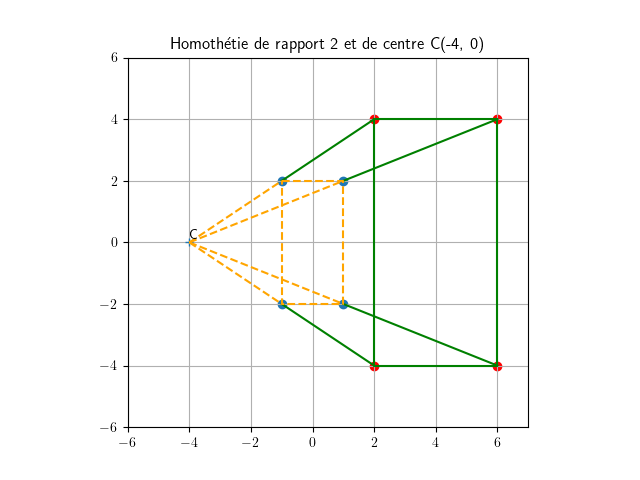
\includegraphics[width=\textwidth]{homothetie.png}
   \caption{Représentation graphique d'une homothétie de centre O}
   \label{fig:homothetie}
 \end{figure}

\begin{prop}
  Soient \(t\) une translation et \(h\) une homothétie de rapport \(\lambda\), alors
  \begin{itemize}
  \item pour tous point \(A\) et \(B\), si \(A'=t(A)\) et si \(B'=t(B)\) alors \(\vect{A'B'}=\vect{AB}\). On dit que \(t\) conserve les distances, \(t\) est une isométrie;
  \item soient \(A\) et \(B\) des points, si \(A'=h(A)\) et si \(B'=h(B)\) alors \(\vect{A'B'}=\lambda\vect{AB}\);
  \item soit \(\Dr\) une droite, alors \(t(\Dr)\) et \(h(\Dr)\) sont des droites parallèles à \(\Dr\).
  \end{itemize}
\end{prop}
\begin{proof} On ne démontre que le troisième point. \(\Dr\) est la droite passant par \(A\) de vecteur directeur \(\vv\) et \(t\) est la translation de vecteur \(\vu\) alors
  \begin{equation}
    t(\Dr)=\enstq{M \in \P}{\exists N \in \Dr \quad \vect{NM}=\vu}.
  \end{equation}
Or \(N \in \Dr \iff \exists \alpha \in \R \ \vect{AN}=\alpha \vv\), donc
\begin{align}
    t(\Dr)&=\enstq{M \in \P}{\exists \alpha \in \R \quad \vect{AM}-\alpha \vv=\vu}\\
    &=\enstq{M \in \P}{\exists \alpha \in \R \quad \vect{AM}=\alpha \vv+\vu}.
  \end{align}
  Comme \(\vect{At(A)}=\vu\), on peut écrire que 
\begin{equation}
  t(\Dr)=\enstq{M \in \P}{\exists \alpha \in \R \quad \vect{t(A)M}=\alpha \vv}.
\end{equation}
L'ensemble \(t(\Dr)\) est donc la droite passant par \(t(A)\) de vecteur directeur \(\vv\), donc elle est parallèle à \(\Dr\).

L'application \(h\) est une homothétie de centre \(\Omega\) et de rapport \(\lambda\), alors
\begin{align}
  h(\Dr)&=\enstq{M \in \P}{\exists N \in \Dr \quad \vect{\Omega M}=\lambda \vect{\Omega N}}\\
    &=\enstq{M \in \P}{\exists \alpha \in \R \quad \vect{\Omega M}=\lambda \vect{\Omega A}+\lambda\alpha \vv}.
\end{align}
Comme \(\vect{\Omega h(A)}=\lambda \vect{\Omega A}\) on peut écrire que 
\begin{equation}
  h(\Dr)=\enstq{M \in \P}{\exists \alpha \in \R \quad \vect{h(A) M}=\lambda\alpha \vv}.
\end{equation}
L'ensemble \(h(\Dr)\) est la droite passant par \(h(A)\) de vecteur directeur \(\vv\) (\(\lambda \neq 0\)) donc elle est parallèle à \(\Dr\).
\end{proof}
\begin{theo}[Théorème de Thalès]
  Soient \(\Dr\) et \(\Dr'\) deux droites sécantes en un point \(\Omega\), \(A\) et \(B\) deux points distincts de \(\Dr\), \(A'\) et \(B'\) deux points distincts de \(\Dr'\). Alors
  \begin{equation}
    (AA') \parallel (BB') \iff \frac{\overline{\Omega B}}{\overline{\Omega A}}=\frac{\overline{\Omega B'}}{\overline{\Omega A'}}=\frac{\overline{BB'}}{\overline{AA'}}
  \end{equation}
\end{theo}
\begin{proof}
  Soit \(h\) l'homothétie de centre \(\Omega\) et de rapport \(\frac{\overline{\Omega B}}{\overline{\Omega A}}\), \(h(A)=B\). L'image par \(h\) de la droite \((AA')\) est une droite passant par \(B\) et parallèle à \((AA')\).

Si \((AA')\) et \((BB')\) sont parallèles, alors la droite \((BB')\) est l'image par \(h\) de la droite \((AA')\). \(A' \in \Dr'\) et \(A' \in (AA')\) donc \(h(A') \in h(\Dr')=\Dr'\) et \(h(A') \in h(AA') = (BB')\) ainsi \(h(A')\) est le point d'intersection de \(\Dr'\) et de \((BB')\) : \(h(A')=B'\). D'où \(\frac{\overline{\Omega B}}{\overline{\Omega A}}=\frac{\overline{\Omega B'}}{\overline{\Omega A'}}\).

Si \(\frac{\overline{\Omega B}}{\overline{\Omega A}}=\frac{\overline{\Omega B'}}{\overline{\Omega A'}}\) alors \(h(A')=B'\) d'où \(h(AA')=(BB')\). Or \(h(AA')\) est une droite parallèle à \((AA')\), donc \((AA')\) est parallèle à \((BB')\).
\end{proof}

\subsection{Rotations}

\begin{defdef}
  Soient \(\Omega\) un point d'affixe \(\omega\) et \(\alpha \in \R\). La rotation de centre \(\Omega\) d'angle \(\alpha\) est l'application définie comme 
\begin{equation}
\fonction{R}{\P}{\P}{M}{M' \norme{\vect{\Omega M}}= \norme{\vect{\Omega M'}} \ \congru{(\vect{\Omega M},\vect{\Omega M'})}{\alpha}{2\pi}}.
\end{equation}
 Elle est représentée dans le plan complexe par \(\fonction{R'}{\C}{\C}{z}{\e^{\ii \alpha}(z-\omega) + \omega}\).
\end{defdef}
\begin{prop}
  Soient des points \(A\) et \(B\), \(r\) une rotation telle que \(A'=r(A)\), \(B'=r(B)\) et \(A'B'=AB\). C'est une isométrie.
\end{prop}

\subsection{Similitudes}

Une similitude directe est une transformation représenté par une application de la forme \(z \longmapsto az+b\) avec \(a\) un complexe non nul et \(b\) un complexe quelconque. Si \(a=1\) alors c'est une translation de vecteur d'affixe \(b\), sinon il existe un unique point fixe appelé centre noté \(\Omega\). Si on note \(h=h_{\Omega, \abs{a}} \ r=r_{\Omega, \Arg{a}}\) alors \(s=r \circ h=h \circ r\).

En particulier, si \(\abs{a}=1\) c'est une rotation, si \(a \in \R\), c'est une homothétie de rapport \(a\).

\begin{prop}
  Une similitude directe conserve les angles et les rapports de distances.
\end{prop}
\begin{proof}
  Soient une similitude \(s : z \longmapsto az+b\) avec \(a \neq 0\), les points \(A_1,A_2,A_3,A_4\) tels que \(A_1 \neq A_3\) et \(A_2 \neq A_4\), on note avec des primes leurs images par \(s\). Alors
  \begin{equation}
    \congru{(\vect{A_1 A_3};\vect{A_2 A_4})}{\Arg\left(\frac{z_4-z_2}{z_3-z_1}\right)}{2\pi},
  \end{equation}
et aussi
\begin{align}
    &\congru{(\vect{A'_1 A'_3};\vect{A'_2 A'_4})}{\Arg\left(\frac{z'_4-z'_2}{z'_3-z'_1}\right)}{2\pi}\\
    \iff&\congru{(\vect{A'_1 A'_3};\vect{A'_2 A'_4})}{\Arg\left(\frac{a(z_4-z_2)}{a(z_3-z_1)}\right)}{2\pi}\\
    \iff&\congru{(\vect{A'_1 A'_3};\vect{A'_2 A'_4})}{(\vect{A_1 A_3};\vect{A_2 A_4})}{2\pi}.
  \end{align}
  On a aussi
\begin{equation}
  \frac{A'_2A'_4}{A'_1A'_3}=\frac{\abs{z'_4-z'_2}}{\abs{z'_3-z'_1}}=\frac{\abs{z_4-z_2}}{\abs{z_3-z_1}}=\frac{A_2A_4}{A_1A_3}.
\end{equation}
\end{proof}

\begin{prop}
  Soient \([AB]\) et \([A'B']\) deux segments de longueur non nulle. Il existe une unique similitude directe \(s\) telle que \(s(A)=A'\) et \(s(B)=B'\).
\end{prop}

\chapter{Courbes planes paramétrées}
\label{chap:courbesparam}
\minitoc
\minilof
\minilot
\section{Préliminaire}
\label{sec:prelim}
\subsection{Notations et interprétations cinématiques}
\label{subsec:not}
On fixe pour tout le chapitre un repère orthonormal direct \(\Rep=(O,\vi,\vj)\) du plan. On identifie le plan à \(\R^2\), un point M à ses coordonnées dans \((O,\vi,\vj)\), un vecteur \(\vu\) à ses coordonnées \((x,y)\) dans \(\Rep\).
\begin{defdef}
 On appelle arc paramétré la donnée de
 \begin{itemize}
 \item un intervalle réel \(I\);
 \item une application \(\fonction{f}{I}{\R^2}{t}{(x(t),y(t))}\).
 \end{itemize}
On supposera que la fonction \(f\) est de classe \(\classe{1}\), c'est-à dire-que \(f\) est dérivable et sa dérivée est continue. Cela signifie que \(x\) et \(y\) sont aussi \(\classe{1}\).
\end{defdef}
%
\subsubsection{Notation}
Pour tout réel \(t\) de \(I\), on considère \(f(t)=(x(t),y(t))\) comme un vecteur (le vecteur de coordonnées \((x(t),y(t))\)). On notera \(M(t)\) le point de coordonnées \((x(t),y(t))\), c'est-à-dire tel que \(\vect{OM}(t)=f(t)\). On notera \(\derived{\vect{OM}}{t}(t)=(x'(t),y'(t))\) et \(\deriveds{\vect{OM}}{t}(t)=(x''(t),y''(t))\) lorsque les dérivées et les dérivées secondes existent.
%
\subsubsection{Interprétation cinématique}
Si \(M(t)\) représente la position d'un point mobile au temps, \(\derived{\vect{OM}}{t}(t)\) est le vecteur vitesse au temps \(t\), et \(\deriveds{\vect{OM}}{t}(t)\) est le vecteur accélération au temps \(t\). On notera \(\Gamma=f(I)=\enstq{f(t)}{t \in I}\) sa trajectoire. On dit que \(\Gamma\) est la courbe paramétrée par \((I,f)\).
%
\subsection{Arcs en coordonnées polaires}
Le point \(M(t)\) peut être donné par un système de coordonnées polaire \((\rho(t),\theta(t))\). Là encore on suppose que les applications \(\rho\) et \(\theta\) sont au moins de classe \(\classe{1}\) sur un intervalle \(I\). Pour tout réel \(t\) de \(I\) on a \(\vect{OM}(t)=f(t)=\rho(t)\vect{u_\theta}(t)\), soit en coordonnées cartésiennes \(M(t)(\rho(t)\cos\theta(t);\rho(t)\sin\theta(t))\).
\begin{prop}
  Les applications \(\fonction{\vu}{\R}{\R^2}{\theta}{\vect{u_\theta}}\) et \(\fonction{\vv}{\R}{\R^2}{\theta}{\vect{v_\theta}}\) sont dérivables et
  \begin{equation}
    \derived{\vu}{\theta}(\theta)=\vect{v_\theta} \quad \derived{\vv}{\theta}(\theta)=-\vect{u_\theta}.
  \end{equation}
\end{prop}
\begin{proof}
  Pour tout réel \(\theta\), on peut identifier \(\vect{u_\theta}\) et \(\vect{v_\theta}\) à leur coordonnées, soit
  \begin{equation}
    \forall \theta \in \R \quad \vect{u_\theta}=(\cos \theta, \sin \theta) \ \vect{v_{\theta}}=(-\sin \theta, \cos \theta).
  \end{equation}
  Puisque les applications sinus et cosinus sont dérivables sur \(\R\), et que pour tout réel \(\theta\), on a \(\sin' \theta=\cos \theta\) et \(\cos' \theta = -\sin \theta\).
\end{proof}

\subsubsection{Calcul du vecteur vitesse}
Supposons que \(f\) et \(\theta\) soit de classe \(\classe{1}\), alors
\begin{align}
  \forall t \in I \quad \vect{OM}(t)&=\rho(t) \vect{u_\theta}=\rho(t)\cos \theta(t) \vi + \rho(t)\sin \theta(t) \vj \\
  \forall t \in I \quad \derived{\vect{M}}{t}(t)&=(\rho'(t) \cos \theta(t) - \rho(t) \theta'(t) \sin \theta(t)) \vi \\
  &+ (\rho'(t) \sin \theta(t) - \rho(t) \theta'(t) \cos \theta(t)) \vj \\
  &=\rho'(t) (\cos \theta(t) \vi + \sin\theta(t) \vj) \\
  & + \rho(t)\theta'(t)(-\sin\theta(t)\vi + \cos\theta(t)\vj)\\
  &=\rho'(t)\vect{u_\theta} + \rho(t)\theta'(t)\vect{v_\theta}.
\end{align}
Tout se passe comme si on dérivait un produit, mais il s'agit ici d'un produit d'une fonction à valeurs réelles par une fonction à valeurs vectorielles, il n'existe pas de théorèmes généraux. Finalement on a~:
\begin{equation}
  \derived{\vect{OM}}{t} = \rho' \vect{u_\theta} + \rho \theta' \vect{v_\theta}.
\end{equation}

\subsubsection{Calcul de l'accélération}
On suppose que \(\rho\) et \(\theta\) sont de classe \(\classe{2}\) sur l'intervalle \(I\). Soit un réel \(t\) de \(I\), alors de la même manière que pour le calcul du vecteur vitesse on arrive à
\begin{equation}
  \deriveds{\vect{OM}}{t}=(\rho''-\rho\theta'^2)\vect{u_\theta} + (2\rho'\theta'+\rho\theta'')\vect{v_\theta}.
\end{equation}

\subsection{Calculs utiles}
Soient \(\fonction{\vect{f}}{I}{\R^2}{t}{(x(t),y(t))}\) et \(\fonction{\vect{g}}{I}{\R^2}{t}{(X(t),Y(t))}\) deux applications de classe \(\classe{1}\).

\subsubsection{Dérivée du produit scalaire}
Soit \(\fonction{\varphi}{I}{\R}{t}{\vect{f}(t) \cdot \vect{g}(t)}\), alors \(\varphi\) vaut
\begin{equation}
  \forall t \in I \quad \varphi(t)=x(t)X(t)+y(t)Y(t).
\end{equation}
Comme \(\varphi\) est la somme de deux fonctions dérivables, elle est dérivable. On calcule
\begin{align}
  \forall t \in I \quad \varphi'(t)&=x'(t)X(t)+x(t)X'(t)+y'(t)Y(t)+y(t)Y'(t)\\
  &=\vect{f'}(t)\vect{g}(t)+\vect{f}(t)+\vect{g'}(t).
\end{align}
On a bien vérifié
\begin{equation}
  (\vect{f} \cdot \vect{g})'=\vect{f'} \cdot \vect{g} + \vect{f} \cdot \vect{g'}.
\end{equation}

\subsubsection{Dérivée de la norme}
Soit \(\fonction{\psi_f}{I}{\R}{t}{\sqrt{\vect{f} \cdot \vect{f}}}\). Par composition d'applications dérivables, \(\psi_f\) est dérivable en tout instant \(t\) où \(\vect{f}(t) \neq \vect{0}\). En un tel instant \(t\), on a
\begin{equation}
  \psi_f'(t)=\frac{2 \vect{f'}(t)\cdot\vect{f}(t)}{2 \sqrt{\vect{f} \cdot \vect{f}}}=\frac{\vect{f}(t)\cdot\vect{f'}(t)}{\norme{\vect{f}}(t)}.
\end{equation}
On a bien vérifié que
\begin{equation}
 \norme{f}'=\frac{\vect{f} \cdot \vect{f'}}{\norme{\vect{f}}}.
\end{equation}

\subsubsection{Dérivée du déterminant}
Soit \(\fonction{\Phi}{I}{\R}{t}{\Det(\vect{f}(t),\vect{g}(t))}\). Soit un réel \(t\) de \(I\), alors
\begin{equation}
 \Phi(t)=x(t)Y(t)-y(t)X(t).
\end{equation}
On voit là que \(\Phi\) est dérivable sur \(I\), puisque c'est une composée de sommes et produits d'applications qui le sont, et
\begin{align}
 \Phi'(t)&=x'(t)Y(t)+x(t)Y'(t)-y'(t)X(t)-y(t)X'(t)\\
 &= \Det(\vect{f'}(t),\vect{g}(t)) + \Det(\vect{f}(t),\vect{g'}(t)).
\end{align}
On a bien vérifié
\begin{equation}
 \Det(\vect{f},\vect{g})'=\Det(\vect{f'},\vect{g}) + \Det(\vect{f},\vect{g'}).
\end{equation}

\section{Arcs paramétrés}
On se fixe dans cette partie un arc paramétré \((I,f)\) avec \(f\) de classe au moins \(\classe{1}\). On note \(\Gamma=f(I)\) et \(M(t)\) le point de coordonnées \(f(t)=(x(t),y(t))\).
\subsection{Étude locale}
Soit \(t_0 \in I\) et \(M_0=f(t_0)\).
\begin{defdef}
 On dit que l'arc \((I,f)\) est régulier en \(t_0\) (ou encore \(M_0\) est un point régulier) si \(\derived{\vect{OM}}{t}(t_0) \neq 0\), alors la courbe \(\Gamma\) admet une tangente au point \(M_0\) dirigée par le vecteur \(\derived{\vect{OM}}{t}(t_0)\).% La figure~\ref{fig:pointreg} illustre cette propriété.
\end{defdef}
\begin{defdef}
 On dit que l'arc \((I,f)\) est birégulier en \(_0\) si les vecteurs \(\derived{\vect{OM}}{t}(t_0)\) et \(\deriveds{\vect{OM}}{t}(t_0)\) ne sont pas colinéaires. La courbe \(\Gamma\) au voisinage de \(M_0\) est du même coté de la tangente en \(M_0\) que le vecteur \(\deriveds{\vect{OM}}{t}(t_0)\). On dit qu'elle \og tourne sa concavité\fg{} vers le vecteur accélération.
\end{defdef}
\begin{prop}
 Le point \(M_0\) est birégulier si et seulement si
 \begin{equation}
  \Det\left(\derived{\vect{OM}}{t}(t_0),\deriveds{\vect{OM}}{t}(t_0)\right) \neq 0,
 \end{equation}
 c'est-à-dire si et seulement si
 \begin{equation}
  x'(t_0)y''(t_0) - x''(t_0)y'(t_0) \neq 0.
 \end{equation}
\end{prop}
On peut généraliser la dernière proposition en écrivant que~: si on suppose que \(p\) et \(q\) sont deux entiers les plus petits possibles tels que \(p<q\) et \(\dfrac{\D^p \vect{OM}}{\D t^p}(t_0)\) et \(\dfrac{\D^q \vect{OM}}{\D t^q}(t_0)\) ne sont pas colinéaires. \(p=\min\enstq{k\geqslant 1}{\dfrac{\D^k \vect{OM}}{\D t^k}(t_0) \neq 0}\) et \(q=\min\enstq{k\geqslant p+1}{\dfrac{\D^k \vect{OM}}{\D t^k}(t_0) \text{~n'est pas colinéaire à~} \dfrac{\D^p \vect{OM}}{\D t^p}(t_0)}\). Alors~:
\begin{itemize}
\item si \(p\) est impair et \(q\) est pair alors c'est un point birégulier,
\item si \(p\) et \(q\) sont impairs alors c'est un point d'inflexion,
\item si \(p\) est impair et \(q\) est pair alors c'est un point de rebroussement de première espèce,
\item si \(q\) et \(p\) sont pairs alors c'est un point de rebroussement de deuxième espèce.
\end{itemize}
En pratique, en un point régulier, \(x'(t_0)\) ou \(y'(t_0)\) est non nul.
\begin{itemize}
\item si \(x'(t_0)=0\) et \(y'(t_0) \neq 0\), la tangente en \(M_0\) est verticale;
\item si \(x'(t_0) \neq 0\) et \(y'(t_0) = 0\), la tangente en \(M_0\) est horizontale;
\item si \(x'(t_0) \neq 0\) et \(y'(t_0) \neq 0\), la tangente en \(M_0\) est de pente \(\frac{y'(t_0)}{x'(t_0)}\).
\end{itemize}
On est amené à étudier les dérivées de \(x\) et de \(y\) afin de déterminer les points singuliers éventuels et leur allure, les tangentes horizontales et verticales.

\subsection{Étude aux bornes}
Soit maintenant une borne \(\alpha\) de l'intervalle I (\(\alpha \in \bar{\R}\)).

\subsubsection{Limite finie}
Si \(\lim\limits_{t \to \alpha}{x(t)}=x_0\) et \(\lim\limits_{t \to \alpha}{y(t)}=y_0\) avec \((x_0,y_0) \in \R^2\), la courbe se rapproche du point \(M_0\) quand \(t\) tend vers \(\alpha\), mais sans l'atteindre \emph{a priori}. On étudie l'existence d'une éventuelle tangente à \(\Gamma\) en considérant le rapport \(\frac{y(t)-y_0}{x(t)-x_0}\).
\begin{itemize}
\item Si \(\lim\limits_{t \to \alpha}\frac{y(t)-y_0}{x(t)-x_0}=p \in \R\) alors la courbe admet une tangente de pente \(p\);
\item sinon la limite est infinie et alors la courbe admet une tangente verticale.
\end{itemize}

\subsubsection{Branche infinie}
On dit que \(\Gamma\) admet une branche infinie quand \(t\) tend vers \(\alpha\) si \(\norme{\vect{OM}(t)}\) tend vers l'infini. En pratique, la courbe présente une branche infinie quand \(x\) ou \(y\) tend vers l'infini. On considère le vecteur \(\frac{\vect{OM}(t)}{\norme{\vect{OM}(t)}}\) (qui est unitaire). S'il existe un réel \(\theta\) tel que ce dernier vecteur tend vers \(\vect{u_\theta}\) alors la courbe \(\Gamma\) admet la direction asymptotique de \(\vect{u_\theta}\). En pratique, on étudie la limite du rapport \(\frac{y(t)}{x(t)}\); si le rapport tend vers un réel \(p\) alors on dit que la courbe \(\Gamma\) admet une direction asymptotique de pente \(p\), sinon la courbe admet une branche asymptotique verticale.

S'il existe une droite \(\Dr\) telle que la limite de la distance entre la courbe est la droite est nulle en \(t \to \alpha\), alors la droite \(\Dr\) est asymptote à la courbe en \(\alpha\). Si la courbe admet une asymptote de pente \(p\), on forme alors le terme \(y(t)-px(t)\), si sa limite est un réel \(m\) en \(\alpha\) alors l'asymptote a pour équation \(y=px+m\) et si sa limite est infinie alors la courbe admet une branche parabolique de direction asymptotique de pente \(p\) mais ce n'est pas une asymptote. Si le rapport a une limite infinie et si \(x\) tend vers un réel \(c\) alors la courbe admet une asymptote d'équation \(x=c\) et si \(x\) tend vers l'infini alors la courbe admet une branche parabolique de direction asymptotique verticale.

Le prolongement naturel de cette étude consiste à étudier la positon de la courbe \(\Gamma\) par rapport à l'asymptote \(\Delta\). Si l'équation de l'asymptote est \(y=px+m\) alors on étudie le signe de \(y(t)-px(t)-m\). Si on a une asymptote d'équation \(x=c\) alors on étudie le signe de \(x(t)-c\).

\subsection{Étude des symétries}
Afin de réduire l'intervalle d'étude, on cherche des symétries de \(\Gamma\), c'est-à-dire des transformations qui la laissent globalement invariante. Soient \(J_1\) et \(J_2\) deux sous-intervalles de \(I\), \(\Psi:J_2 \longmapsto J_1\) une application continue bijective telle que \(\Psi^{-1}\) soit continue. On note \(\Gamma_1=(J_1,f_{|J_1})\) et \(\Gamma_2=(J_2,f_{|J_2})\). En pratique \(\Psi\) sera de la forme \(\Psi(t)=t+\tau\), \(\Psi(t)=-t\), \(\Psi(t)=\frac{1}{t}\) et le reste. Suivant d'éventuelle formule liant \(f(\Psi(A))\) et \(f(t)\) on déduit la courbe \(\Gamma_2\) de la courbe \(\Gamma_1\) par une bonne transformation, un tableau de ces transformations est donné en table~\ref{tab:sym}.

\begin{table}
 \centering
 \begin{tabular}{|c|c|} \hline
  sur \( J_2\) & transformation \\ \hline
  \(x \circ \Psi=\Id \quad y \circ \Psi=\Id\) &Identité \\ \hline
  \(x \circ \Psi=\Id \quad y \circ \Psi=-\Id\) &Symétrie d'axe \((Ox)\) \\ \hline
  \(x \circ \Psi=-\Id \quad y \circ \Psi=\Id\) &Symétrie d'axe \((Oy)\) \\ \hline
  \(x \circ \Psi=\Id+a \quad y \circ \Psi=\Id+b\) & Translation de vecteur \(\vu(a,b)\)\\ \hline
  \(x \circ \Psi=y \quad y \circ \Psi=x\) & Symétrie / première bissectrice\\ \hline
  \(x \circ \Psi=-y \quad y \circ \Psi=-x\) & Symétrie / origine\\ \hline
 \end{tabular}
 \caption{Symétries possibles}
 \label{tab:sym}
\end{table}

\subsection{Plan d'étude globale}
\begin{enumerate}
\item Domaine de définition de \(f\) : \(Df=Dx \cap Dy\)
\item Restriction du domaine d'étude par la recherche de symétries
\item Étude des variations de \(x\) et \(y\) (recherche d'éventuels points singuliers et de tangentes)
\item Étude aux bornes
\item Tracé de la courbe, le morceau étudié complété par symétrie
\item Éventuellement, rechercher les points multiples (c'est-à-dire les points où la courbe se recoupe elle-même). On se place sur un intervalle \(I\) avec lequel on obtient toute la courbe. On regarde s'il existe \((u,v) \in I^2\) avec \(u \neq v\) et \(M(u)=M(v)\). On définit particulièrement la notion de point double, ou triple.
\end{enumerate}

\subsection{Folium de Descartes}\index{folium}
Le folium est une courbe paramétrée définie telle que
\begin{equation}
 x(t) = \frac{t}{1+t^3} \qquad y(t)=\frac{t^2}{1+t^3}
\end{equation}
Le domaine de définition de cette courbe est \(D_f = \R\setminus\{-1\}\). Pour tout réel non nul de \(D_f\) on a \(x\left(\frac{1}{t}\right)=y(t)\) et \(y\left(\frac{1}{t}\right)=x(t)\) alors on peut travailler dans \(I=\intervalleoo{-1}{1}\) et on obtiendra le reste par symétrie par rapport à la première bissectrice. Les composantes de la courbe, \(x\) et \(y\), sont dérivables sur \(I\) et on a pour tout \(t \in I\)
\begin{equation}
 x'(t)=\dfrac{1-2t^3}{(1+t^3)^2} \qquad y'(t)=\dfrac{t(2-t^3)}{(1+t^3)^2}.
\end{equation}
Alors pour tout \(t \in I\), on a~:
\begin{equation}
 x'(t)=0 \iff t=\sqrt[3]{\frac{1}{2}} \qquad y'(t)=0 \iff t=0.
\end{equation}
Tous les points sont donc réguliers.
\begin{itemize}
\item En \(t=0\), \(x(0)=y(0)=0\) et \(y'(0)=0\), la tangente est horizontale;
\item en \(t=t_0=\sqrt[3]{\frac{1}{2}}\),  \(x(t_0)=\frac{2^{2/3}}{3} \approx 0.53\) et \(y(t_0)=\frac{2^{1/3}}{3}\approx 0.42\), la tangente est verticale.
\end{itemize}

Le tableau de variation de cette courbe paramétrée est donnée par le tableau~\ref{tab:folium}.

%\begin{table}
%\centering
% \variations
%t   &  & -1   &     & 0  &   & t_0=\sqrt[3]{\frac{1}{2}}        &    & 1        \\
%x'(t) &\bg &    &  +   &   &   & \z                    &  -  &         \\
%x   &\bg &\b{\mI} & \tcb   & 0  & \ch & \h{\frac{2}{3} \sqrt[3]{\frac{1}{2}}}  & \d   & \b{\frac{1}{2}} \\
%y'(t) &\bg &    &  -   & \z  & +  &                     &    &         \\
%y   &\bg &\h{\pI} & \d    & \b 0 & \tcb & \frac{\sqrt[3]{2}}{3}          & \ch  & \h{\frac{1}{2}} \\
%\fin
%\caption{Tableau de variations de la courbe paramétrée \(\left(\frac{t}{1+t^3},\frac{t^2}{1+t^3}\right)\)}
%\label{tab:folium}
%\end{table}

\begin{table}
    \centering   
    \begin{tikzpicture}
       \tkzTabInit{t / 1, $x'(t)$ / 1 , $x(t)$ / 1, $y'(t)$ / 1, $y(t)$ / 1}{$-1$, $0$, $t_0$, $1$}
       \tkzTabLine{d, +, , +, z, -,}
       \tkzTabVar{D-/ $-\infty$, R , +/ $\frac{2}{3}t_0$, -/ $\frac{1}{2}$}
       \tkzTabVal{1}{3}{0.5}{$0$}{$0$}
       \tkzTabLine{d, +, z, +, ,+ }
       \tkzTabVar{D+/ $+\infty$, -/ $0$, R, +/ $\frac{1}{2}$}
       \tkzTabVal{2}{4}{0.5}{$t_0$}{$\frac{2}{3}t_0^2$}
    \end{tikzpicture}
    \caption{Tableau de variations du folium de Descartes}
    \label{tab:folium}
\end{table}

\emph{Étude aux bornes}~:
ici les bornes à étudier sont \(1\) et \(-1\). Si on étudie le comportement de cette courbe en 1, on remarque que \(x(1)=y(1)=\frac{1}{2}\) et que \(y'(1)=-x'(1)=-\frac{1}{4}\). La tangente est perpendiculaire à la première bissectrice.

L'étude en \(-1\) montre que la courbe admet une branche infinie et si on forme le rapport \(\frac{y}{x}\), on trouve qu'il vaut \(t\) et tend donc vers \(-1\) en \(-1\). Donc la courbe admet une direction asymptotique de pente \(-1\). La différence \(y(t)-px(t)\) avec \(p=-1\) vaut pour tout \(t\) non nul de \(I\) \(y(t)+x(t)\) et tend vers \(-\frac{1}{3}\) donc la courbe admet une asymptote d'équation \(y=-x-\frac{1}{3}\). Puisque le signe de \(y(t)+x(t)+\frac{1}{3}\) est toujours positif, l'asymptote est sous la courbe. La représentation graphique du folium est donnée par la figure~\ref{fig:folium}.
\begin{figure}
 \centering
 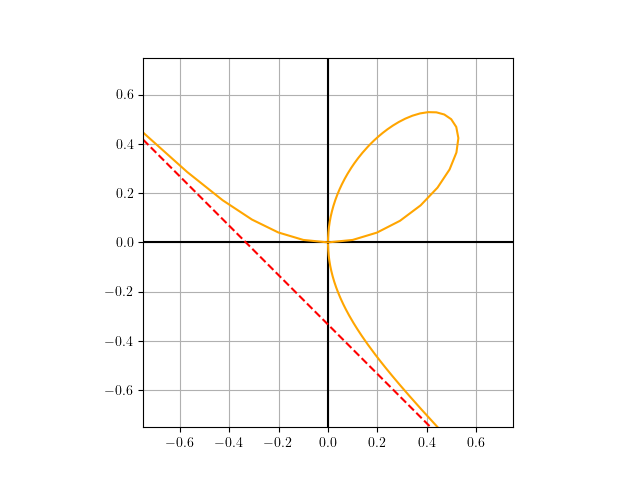
\includegraphics[scale=0.7]{folium.png}
 \caption{Représentation graphique du folium de Descartes}
 \label{fig:folium}
\end{figure}

\emph{Remarque}~:
soit \(\Psi : I \longmapsto \R\) continue et \(\Gamma\) le graphe de \(\Psi\). \(\Gamma\) peut être considérée comme une courbe paramétrée \(x(t)=t \quad y(t)=\Psi(t)\). On définit \(\fonction{f}{I}{\R^2}{t}{(x(t),y(t))}\). Si \(\Psi\) est dérivable alors pour tout réel \(t\) de I on a \(f'(t)=(1;\Psi'(t))\) alors tous les points sont réguliers. Si \(\Psi\) est deux fois dérivable alors \(f\) est deux fois dérivable et pour tout réel \(t\) de I on a \(f''(t)=(0,\Psi''(t))\), alors \(\Det(f'(t),f''(t))=\Psi''(t)\) et donc l'équivalence est vraie
\begin{equation}
 t_0 \text{~est un point birégulier } \iff \Psi''(t_0) \neq 0.
\end{equation}

\section{Courbes en polaires}
Soient I un intervalle de \(\R\), \(r\) une application de I vers \(\R\) au moins de classe \(\classe{1}\). On considère la courbe définie par l'équation polaire \(\rho=r(\theta)\), qu'on étudie comme un arc paramétré par \(\theta\). On note \(M(\theta)\) le point \og courant \fg{}.

\subsection{Étude locale en un point}
\subsubsection{Dérivation}
On sait que \(\theta(t)=\theta \quad \theta'(t)=1 \quad \theta''(t)=0\) alors si \(r\) et deux fois dérivable, en appliquant la formule de la section~\ref{subsec:not} on arrive à
\begin{align}
 \derived{\vect{OM}}{\theta}(\theta)&=r'(\theta) \vu_\theta + r(\theta) \vv_\theta;\\
 \deriveds{\vect{OM}}{\theta}(\theta)&=(r''(\theta)-r(\theta)) \vu_\theta + 2r'(\theta) \vv_\theta.
\end{align}

\subsubsection{Points réguliers}
Pour tout réel \(\theta\) de I,
\begin{equation}
 \derived{\vect{OM}}{\theta}(\theta)=0 \iff
 \begin{cases}
   r'(\theta) = 0 \\ r(\theta)=0
 \end{cases}.
\end{equation}
Tous les points différents du pôle (ou origine) sont réguliers. En un point tel que \(r(\theta) \neq 0\), la courbe \og tourne autour du pôle dans le sens direct \fg{}. Si le rapport \(\frac{r'(\theta)}{r(\theta)}\) est négatif (resp.\ positif) alors \(r(\theta)\) se rapproche (resp.\ s'éloigne) du pôle.

\subsubsection{Points d'annulation}
On suppose ici que \(\theta_0\) est un zéro \emph{isolé} de la fonction \(r\), c'est-à-dire \(r(\theta_0)=0\) et il existe \(\epsilon >0\) tel que pour tout réel \(\theta\) de l'intervalle ouvert \(\intervalleoo{\theta_0-\epsilon}{\theta_0+\epsilon}\setminus\{\theta_0\}\), on a \(r(\theta) \neq 0\)

\begin{prop}[admise]
 Soit \(\theta_0\) un zéro isolé de la fonction \(r\), alors \(\Gamma\) admet pour tangente en \(M(\theta_0)\) la droite \(\Dr_{\theta_0}\). De plus~:
 \begin{enumerate}
 \item si \(r\) change de signe en \(\theta_0\) alors le point est d'allure normale (comme par exemple un cercle qui passe par le pôle);
 \item si \(r\) s'annule sans changer de signe alors le point est un point de rebroussement de première espèce (comme par exemple une cardioïde).
 \end{enumerate}
\end{prop}

\subsection{Étude aux bornes}
\subsubsection{Lorsque \(\theta\) tend vers l'infini}
Si la fonction \(r\) tend vers zéro lorsque \(\theta\) tend vers l'infini, alors le point courant tend vers le pôle. \(\Gamma\) n'admet pas d'asymptote et on dit que le pôle est un \emph{point asymptote}.

Si la fonction \(r\) tend vers un réel \(a\) non nul lorsque \(\theta\) tend vers l'infini, alors la distance du point courant au cercle \(\cercle{0}{\abs{a}}\) tend vers zéro et donc c'est un \emph{cercle asymptote}.

Si par contre la fonction \(r\) tend vers l'infini lorsque \(\theta\) tend vers l'infini, alors la courbe admet une branche infinie sans direction asymptotique, on parle de \emph{branche spirale}.

\subsubsection{Lorsque \(\theta\) tend vers \(\theta_0\)}
Si la fonction \(r\) tend vers une limite finie, il n'y a rien de particulier. Par contre si la fonction \(r\) tend vers l'infini lorsque \(\theta\) tend vers \(\theta_0\), alors la courbe admet une branche infinie de direction asymptotique \(\vu_{\theta_0}\). On analyse s'il y a une asymptote. Pour le faire, on effectue un changement de repère et on se place dans le repère \(\Rep'\) déduit du repère \(\Rep\) par une rotation de centre \(O\) et d'angle \(\theta_0\). Les coordonnées cartésiennes de \(M(\theta)\) dans \(\Rep'\) seront alors
\begin{equation}
  M(\theta)
  \begin{cases}
    X(\theta)=r(\theta)\cos(\theta-\theta_0)\\
    Y(\theta)=r(\theta)\sin(\theta-\theta_0)
  \end{cases}.
\end{equation}
Lorsque \(\theta\) tend vers \(\theta_0\), \(X(\theta)\) tend vers l'infini et \(Y(\theta)\) est une forme indéterminée. Deux cas se présentent~:
\begin{itemize}
\item si \(Y\) tend vers une limite finie \(L\) alors la courbe admet une asymptote d'équation \(y=L\) dans \(\Rep'\);
\item sinon la courbe n'admet pas d'asymptote, le graphe présente une branche parabolique de direction asymptotique \(\vu_{\theta_0}\).
\end{itemize}

\subsection{Symétries}
On cherche de nouveau à réduire l'intervalle d'étude. Une liste non-exhaustive de transformation est donnée dans la table~\ref{tab:sympol}.
\begin{table}
  \centering
  \begin{tabular}{|c|c|}\hline
    Hypothèse & Transformation \\ \hline
    \(r(-\theta)=r(\theta)\) & Symétrie / \((Ox)\) \\ \hline
    \(r(-\theta)=-r(\theta)\) & Symétrie / \((Oy)\) \\ \hline
    \(r(\theta+\alpha)=kr(\theta)\) & Similitude directe de centre O \\ & d'angle \(\alpha\) et de rapport k \\ \hline
    \(r(\alpha-\theta)=r(\theta)\) & Symétrie / droite \(\Dr_{\alpha/2}\) \\ \hline
    \(r(\alpha-\theta)=-r(\theta)\) & Symétrie / droite \(\Dr_{\pi/2 + \alpha/2}\) \\ \hline
 \end{tabular}
 \caption{Table des symétries}
 \label{tab:sympol}
\end{table}
Si la fonction \(r\) est de période \(T\), alors on peut réduire l'intervalle d'étude.
\subsection{Points multiples}\index{multiple}
Le point \(M(\theta)\) est un point multiple si et seulement s'il existe \(\theta' \neq \theta\) tel que \(M(\theta)=M(\theta')\) c'est-à-dire si et seulement si
\begin{align}
 r(\theta)&=r(\theta')=0, \\
 r(\theta)&=r(\theta') \quad \congru{\theta}{\theta'}{2\pi},\\
 r(\theta)&=-r(\theta') \quad \congru{\theta}{\theta'+\pi}{2\pi}.
\end{align}
On se placera sur un intervalle, le plus petit possible, qui permet d'obtenir toute la courbe.
\subsection{Plan d'étude globale}
\begin{enumerate}
\item Ensemble de définition de la fonction \(r\);
\item Restriction du domaine d'étude par la recherche de symétries et périodes;
\item Étude de \(r\)~: variations, signe, points d'annulation, tangentes remarquables;
\item Étude aux bornes;
\item Tracé de la courbe (le morceau étudié puis complétion par symétrie);
\item Éventuellement les points multiples.
\end{enumerate}

\subsection{Exemple}

Soit \(\Gamma\) définie par \(r(\theta)=\cos \theta + \cos 3\theta\). La fonction \(r\) est définie sur \(\R\) tout entier. Elle est \(2\pi\)-périodique, on peut donc restreindre l'étude à \(\intervalleff{-\pi}{\pi}\). Puisque la fonction cosinus est paire, la fonction \(r\) est aussi paire, on peut donc encore restreindre le domaine d'étude à \(\intervalleff{0}{\pi}\) et ensuite on complétera la courbe par une symétrie d'axe \((Ox)\). Pour tout réel \(\theta \in \intervalleff{0}{\pi}\) on a \(r(\pi-\theta)=-r(\theta)\) alors on peut restreindre l'étude sur \(\intervalleff{0}{\frac{\pi}{2}}\) puis on complète par une symétrie d'axe \(\Dr_{\pi/2+\pi/2}\) c'est-à-dire \((Ox)\). On fait deux fois la même symétrie, cela signifie qu'on obtient toute la courbe pour \(\theta \in \intervalleff{0}{\pi}\). Au final le domaine d'étude est restreint à \(\intervalleff{0}{\frac{\pi}{2}}\)

Soit \(\theta \in \intervalleff{0}{\frac{\pi}{2}}\), alors \(r(\theta)=\cos \theta + \cos 3\theta=2\cos(2\theta)\cos \theta\) d'après les transformations produit en somme. Donc
\begin{equation}
  r(\theta)=0 \iff \cos(2\theta)=0 \text{~ou~} \cos \theta=0 \iff \theta \in \left\{\frac{\pi}{4}; \frac{\pi}{2}\right\}.
\end{equation}
La fonction \(r\) est dérivable sur \(\intervalleff{0}{\frac{\pi}{2}}\). Pour tout \(\theta \in \intervalleff{0}{\frac{\pi}{2}}\), on a
\begin{equation}
 r'(\theta)=-\sin\theta - 3 \sin(3 \theta).
\end{equation}
De plus on sait que \(\sin(3 \theta) = \Im(\e^{\ii 3\theta})\) et
\begin{equation}
 \e^{\ii 3 \theta}=\cos^3 \theta + 3\cos^2 \theta \ii \sin \theta + 3 \cos \theta \ii^2 \sin^2 \theta + \ii^3\sin^3 \theta.
\end{equation}
 Ainsi \(\sin(3 \theta) = 3 \sin\theta \cos^2 \theta - \sin^3 \theta\). En introduisant \(\sin^2=1-\cos^2\) dans l'équation et en factorisant, on arrive à
 \begin{equation}
  r'(\theta)=2 \sin \theta (1-6 \cos^2 \theta).
 \end{equation}
Alors
\begin{equation}
 r'(\theta)=0 \iff \sin\theta=0 \text{~ou~} \cos^2 \theta = \frac{1}{6} \iff \theta \in \left\{0, \arccos\left(\frac{1}{\sqrt{6}}\right)\right\}.
\end{equation}
\begin{itemize}
\item En \(\frac{\pi}{4}\), on a \(r\left(\frac{\pi}{4}\right)=0\) et \(r'\left(\frac{\pi}{4}\right)=-2\sqrt{2}\) et donc \(\derived{\vec{M}}{\theta}\left(\frac{\pi}{4}\right) = -2\sqrt{2}\vec{u}_{\frac{\pi}{4}}\) La tangente est donc la première bissectrice;
\item en \(\theta_0=\arccos\left(\frac{1}{\sqrt{6}}\right)\), on a \(r'(\theta_0)=0\) et
 \begin{align}
  r(\theta_0) & = \cos(\theta_0) + \cos(3 \theta_0) \\
  & = \frac{1}{\sqrt{6}} + \cos^3\theta_0 - 3 \sin^2\theta_0 \cos\theta_0 \\
  & = \frac{\sqrt{6}}{6} \left(1+\frac{1}{6}-3\left(1-\frac{1}{6}\right)\right) \\
  & = -\frac{2\sqrt{6}}{9}
 \end{align}
En \(\theta_0\), la tangente est perpendiculaire à \((OM(\theta_0))\).
\end{itemize}
\begin{itemize}
\item En \(0\), \(r'(0)=0\) et \(r(0)=2\) et donc \(\derived{\vec{M}}{\theta}(0)=2 \vec{v}_0=2 \vj\), la tangente est parallèle à \((Oy)\);
\item En \(\frac{\pi}{2}\), \(r\left(\frac{\pi}{2}\right)=0\) et \(r'\left(\frac{\pi}{2}\right)=2\) et donc \(\derived{\vec{M}}{\theta}\left(\frac{\pi}{2}\right)=2 \vec{v}_0=2 \vj\), la tangente est parallèle à \((Oy)\).
\end{itemize}

Le tableau de variations est donnée par le tableau \ref{tab:gamma}.

\begin{table}
    \centering   
    \begin{tikzpicture}
       \tkzTabInit{$\theta$ / 1, $r'(\theta)$ / 1 , $r$ / 1}{$0$, $\frac{\pi}{4}$, $\theta_0$, $\frac{\pi}{2}$}
       \tkzTabLine{z, -, , -, z, +,}
       \tkzTabVar{+/ $2$, R , -/ $r(\theta_0)$, +/ $0$}
%       \tkzTabVal{1}{3}{0.5}{$0$}{$0$}
%       \tkzTabLine{d, +, z, +, ,+ }
%       \tkzTabVar{D+/ $+\infty$, -/ $0$, R, +/ $\frac{1}{2}$}
%       \tkzTabVal{2}{4}{0.5}{$t_0$}{$\frac{2}{3}t_0^2$}
    \end{tikzpicture}
    \caption{Tableau de variations de $\Gamma$}
    \label{tab:gamma}
\end{table}

On trace cette courbe paramétrée sur la figure~\ref{fig:pol}.
\begin{figure}
 \centering
 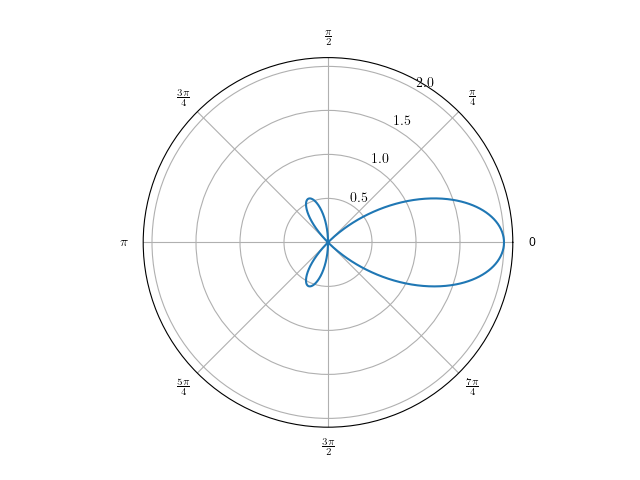
\includegraphics[scale=0.85]{courbepolaire.png}
 \caption{Courbe polaire $\Gamma$ définie par \(r(\theta)=\cos\theta+\cos(3\theta)\)}
 \label{fig:pol}
\end{figure}
\section{Exercices}
\begin{exercice}[Astroïde]
    Soit un réel \(a > 0\) fixé. Tracer la courbe paramétrée par \(x(t) = a \cos^3 t, y(t) = a \sin^3(t)\) pour \(t \in \R\). On étudiera en particulier les axes de symétries.
\end{exercice}
\begin{exercice}
    Tracer la courbe paramétrée par \(x(t) = \tan t + \sin t, y(t) = \frac{1}{\cos t}\). On précisera en particulier la nature de son point de rebroussement et de ses branches infinies.
\end{exercice}
\begin{exercice}
    Soit \(\mathcal{C}\) la courbe paramétrée par \(x(t) = t^4 - t^3 - t^2, y(t) = t^4 + t^3 + t^2\) pour \(t \in \R\).
    \begin{enumerate}
        \item Donner un paramétrage de \(\mathcal{C}\) dans le repère \((O, \vi+\vj,\vj-\vi)\).
        \item Montrer que la courbe admet un unique point non régulier ; préciser sa nature.
        \item Étudier la branches infinies de la courbe.
        \item Donner l'allure de la courbe.
    \end{enumerate}
\end{exercice}
\begin{exercice}[Deltoïde]
    Représenter l'arc défini par le paramétrage \(x(t) = 2 \cos t + cos(2t), y(t) = 2\sin(t) - \sin(2t)\).
\end{exercice}
\begin{exercice}[Cycloïde]
    \begin{enumerate}
        \item Soient \(a>0\) fixé et \(\Gamma_1\) l'arc défini par le paramétrage \(x(t) = a(t-\sin t), y(t) = a(1-\cos t)\). Représenter cet arc. On se demandera en particulier si les points sont biréguliers.
        \item Soient maintenant \(\lambda \in \intervalleoo{0}{+\infty}\) et \(\Gamma_\lambda\) l'arc défini par par le paramétrage \(x(t) = a(t-\lambda \sin t), y(t) = a(1-\lambda \cos t)\). Donner l'allure de cet arc en distinguant les cas \(\lambda >1\) et \(\lambda < 1\).
    \end{enumerate}
\end{exercice}
\begin{exercice}
    On considère l'arc \(\Gamma\) défini par le paramétrage \(x(t) = (1-t)^2\e^t , y(t) = 2(1-t)\e^t\). Représenter \(\Gamma\).
\end{exercice}
\begin{exercice}
    Tracer l'arc \(\Gamma\) défini par l'équation polaire \(\rho = \frac{1}{\cos^3 \frac{\theta}{3}} \). On étudiera en particulier ses symétries et la nature de ses branches infinies.
\end{exercice}
\begin{exercice}
    Tracer l'arc \(\Gamma\) défini par l'équation polaire \(\rho = \frac{1}{\e^{\theta}-1} \). On étudiera en particulier la nature de ses branches infinies et la position de la courbe par rapport à ses asymptotes.
\end{exercice}
\begin{exercice}
    Tracer la courbe d'équation polaire \(\rho = 1 + 2 \cos \theta - 4 \cos^2 \theta \). Préciser en particulier ses points multiples.
\end{exercice}
\begin{exercice}
    Soient \(\mathcal{C}\) un cercle et \(O\) un point fixe du cercle. Pour tout point \(M\) du cercle, on note \((\mathcal{D})\) la tangente au cercle au point \(M\) et \(N\) le symétrique par rapport de \(O\) par rapport à \((\mathcal{D})\). Représenter le lieu du point \(N\) lorsque \(M\) parcourt le cercle et en donner une équation polaire (dans un repère choisi judicieusement).
\end{exercice}
\begin{exercice}
    Tracer la courbe définie par l'équation polaire \(\rho = \frac{1+\sin\theta}{\theta}\).
\end{exercice}

\chapter{Coniques}
\minitoc
\minilof
\minilot
\section{Définition monofocale et équation polaire}
Soient \(F\) un point du plan, \(\Dr\) une droite ne passant pas par \(F\), \(e\) un réel strictement positif.
\subsection{Définition monofocale}
\begin{defdef}
   On appelle conique de foyer \(F\), de directrice \(\Dr\) et d'excentricité \(e\) l'ensemble des points \(M\) du plan tels que
  \begin{equation}
    MF=e MH,
  \end{equation}
  où \(H\) est le projeté orthogonal de \(M\) sur \(\Dr\).
\end{defdef}
\begin{defdef}
  On appelle axe focal de la conique \(\con{e}\) la droite \(\Delta\) perpendiculaire à la droite \(\Dr\) passant par \(F\).
\end{defdef}
\begin{prop}
  La conique \(\con{e}\) est symétrique par rapport à l'axe focal \(\Delta\).
\end{prop}
\begin{proof}
  On note \(K\) le projeté orthogonal de \(F\) sur \(\Dr\) : \(K=D \cap \Delta\). Soit \(M \in \con{e}\) et \(H\) son projeté orthogonal sur \(\Dr\). Soit \(M'\) le symétrique de \(M\) par rapport à \(\Delta\), \(H'\) le projeté orthogonal de \(M'\) sur \(\Dr\) (c'est aussi le symétrique de \(H\) par rapport à \(\Delta\)). Alors
\begin{equation}
  \frac{M'F}{M'H'} = \frac{MF}{MH} = e,
\end{equation}

donc le point \(M'\) appartient à la conique \(\con{e}\).
\end{proof}
Si on considère l'application \(\fonction{\varphi}{P\setminus\{\Dr \cup F\}}{\Rplusetoile}{M}{\frac{MF}{MH}}\), où \(H\) est le projeté orthogonal de \(M\) sur \(\Dr\), les coniques \(\con{e}\) de directrice \(\Dr\) sont les lignes de niveau de \(\varphi\). On cherche les points d'intersection entre \(\con{e}\) et l'axe \(\Delta\). On note \(K\) le projeté orthogonal de \(F\) sur \(\Dr\). On place l'origine des abscisses en \(K\) et on oriente \(\Delta\) de \(K\) vers \(F\), on note \(d=KF\).

Soit M sur \(\Delta\) le point d'abscisse \(x\). Le projeté orthogonal de M sur la directrice \(\Dr\) est le point \(K\), puisque \(\Dr\) et \(\Delta\) sont orthogonales et se croisent en \(K\). On a alors la suite d'équivalence suivante~:
\begin{align}
  M \in \con{e} &\iff MF = e MK \\
  &\iff MF^2=e^2 MK^2 \\
  &\iff (x-d)^2=e^2 x^2\\
  &\iff x^2+d^2-2xd=e^2 x^2\\
  &\iff x^2(1-e^2)-2xd+d^2=0.
\end{align}
On distingue deux cas~:
\begin{itemize}
\item si \(e=1\), alors le point M est sur la conique si et seulement si \(x=\frac{d}{2}\). Il y a donc un unique point d'intersection entre la conique \(\con{1}\) est son axe focal \(\Delta\), c'est le milieu de \([KF]\). Cette conique est une parabole;
\item sinon comme \(1-e^2 \neq 0\), on peut calculer le discriminant de ce trinôme qui vaut \((2de)^2\), alors les deux racines réelles du trinôme sont \(x_1=\frac{d}{1+e}\) et \(x_2=\frac{d}{1-e}\). Soient les points d'intersections \(A_1\) et \(A_2\) de \(\con{e}\) et \(\Delta\), d'abscisse respectives \(x_1\) et \(x_2\). Alors \(\vect{KA}=\frac{1}{1+e} \vect{KF}\) et \(\vect{KA'}=\frac{1}{1-e} \vect{KF}\). On peut distinguer deux sous-cas~:
  \begin{itemize}
  \item si \(e<1\) alors \(x_1\) et \(x_2\) sont positifs et les deux points \(A\) et \(A'\) sont du même côté de \(\Dr\) que \(F\). On dira que \(\con{e}\) est une ellipse;
  \item si \(e>1\) alors \(A\) est du même côté que \(F\) mais \(A'\) est de l'autre, dans ce cas là on dira que \(\con{e}\) est une hyperbole.
  \end{itemize}
\end{itemize}

\subsection{Équation polaire de \(\con{e}\)}
On munit le plan de la base orthonormale \((\vi,\vj)\) où \(\vi=\frac{\vect{FK}}{\norme{\vect{FK}}}\) et où \(\vj\) est tel que \((\vi,\vj)=\frac{\pi}{2}\) et \(\norme{\vj}=1\). On se place dans le repère \(\Rep=(F,\vi,\vj)\). Notons \(d=FK\), une équation de \(\Dr\) dans \(\Rep\) est \(x=d\) et son équation polaire dans \(\Rep\) est \(\rho=\frac{d}{\cos \theta}\). Soient un point \(M\) du plan et son système de coordonnées polaires \((\rho,\theta)\) : \(\vect{FM}=\rho\vect{u}_\theta\), alors~:
\begin{align}
  M \in \con{e} &\iff MF = e MH \\
  &\iff \abs{\rho}=e\abs{d-\rho \cos\theta}\\
  &\iff \begin{cases}\rho = ed-e\rho\cos\theta \\ \text{ou}\\ \rho = e\rho\cos\theta-ed \end{cases} \\
  &\iff  \begin{cases}\rho = \frac{ed}{1+e\cos\theta} \\ \text{ou}\\ \rho = \frac{-ed}{1-e\cos\theta} \end{cases}.
\end{align}
On obtient deux équations polaires, mais ces deux équations sont les mêmes~: en effet, si \((\rho,\theta)\) est un s.c.p.\ de \(M\) alors \(\rho=\frac{ed}{1+e\cos\theta}\) et donc en prenant l'opposé \(-\rho=\frac{-ed}{1-e\cos(\theta+\pi)}\) et donc \((-\rho,\theta+\pi)\), étant un deuxième s.c.p.\ de \(M\) dans \(\Rep\) vérifie la deuxième équation. Alors~:
\begin{equation}
  M(\rho,\theta) \in \con{e} \iff \rho=\frac{ed}{1+e\cos\theta}.
\end{equation}
\(\rho=\frac{ed}{1+e\cos\theta}\) est une équation polaire de la conique \(\con{e}\).
\begin{enumerate}
\item Si on oriente la droite (FK) dans l'autre sens on obtient une équation du même type avec un signe négatif;
\item l'équation est la même pour toutes les valeurs de l'excentricité, mais le domaine dans lequel varie \(\theta\) dépend de l'excentricité.
\end{enumerate}

\section{Équations réduites}
\label{sec:eqred}
Soit \(\con{e}\) la conique de foyer \(F\), de directrice \(\Dr\), d'excentricité \(e\). On note \(d=d(F,\Dr)>0\). On pose \(p=ed\), \(p\) est appelé le paramètre de la conique \(\con{e}\). On se place dans le ROND \((F,\vi,\vj)\) avec \(\vi=\frac{\vect{KF}}{KF}\). Dans ce repère, \(F(0,0), K(-d,0)\) et soit \(M(x,y)\) un point du plan, \(H\) le projeté orthogonal de \(M\) sur \(\Dr\), \(H(-d,y)\). Alors~:
\begin{align}
  M \in \con{e} &\iff MF = e MH \\
  &\iff MF^2 = e^2 MH^2\\
  &\iff x^2+y^2=e^2(x+d)^2.
\end{align}

\subsection{Cas de la parabole}
Soit \(S\) l'unique point d'intersection entre \(\con{1}\) et \(\Delta\). Le point \(S\) est le sommet de la parabole, c'est aussi le milieu de \([KF]\), alors \(S\left(\frac{-d}{2}\right)\). On adopte un nouveau repère~: le ROND \((S,\vi,\vj)\), si \(M\) a pour coordonnées \((x,y)\) dans \((F,\vi,\vj)\) et \((X,Y)\) dans \((S,\vi,\vj)\) alors \(X=x+\frac{d}{2}\) et \(Y=y\). Ainsi~:
\begin{align}
  M(X,Y) \in \con{1} &\iff \left(X-\frac{d}{2}\right)^2+Y^2=\left(X+\frac{d}{2}\right)^2\\
  &\iff \left(X-\frac{d}{2}\right)^2 - \left(X+\frac{d}{2}\right)^2+Y^2=0\\
  &\iff Y^2=2dX=2pX,
\end{align}
puisque \(p=ed=d\).
\begin{theo}
Soit \(\P\) une parabole de foyer \(F\) de directrice \(\Dr\). Il existe un repère orthonormal \((S,\vi,\vj)\) dans lequel \(\P\) a pour équation \(Y^2=2pX\), c'est ce qu'on appelle l'équation réduite de la parabole \(\P\).

Réciproquement, si \(p\) est un réel strictement positif, l'ensemble des points représentés par l'équation cartésienne \(Y^2=2pX\) dans un repère orthonormal \(\rond\) est une parabole de foyer \(F\left(\frac{p}{2},0\right)\), de directrice \(\Dr\) et d'équation \(X=\frac{-p}{2}\). Le nombre \(p\) est le paramètre de la parabole. Un paramétrage de la parabole est~:
  \begin{equation}
    \forall t \in \R \quad
    \begin{cases}
      x(t)=\frac{t^2}{2p} \\
      y(t)=t
    \end{cases}.
  \end{equation}
\end{theo}

Plusieurs paraboles sont représentées sur la figure~\ref{fig:parabole}.

\begin{figure}
    \begin{subfigure}{.5\textwidth}
      \centering
      % include first image
      \includegraphics[scale=.45]{Tracé_parabole_0.5.png}  
      \caption{$p=0.5$}
      \label{fig:parabole1}
    \end{subfigure}
    \begin{subfigure}{.5\textwidth}
      \centering
      % include first image
      \includegraphics[scale=.45]{Tracé_parabole_0.75.png}  
      \caption{$p=0.75$}
      \label{fig:parabole2}
    \end{subfigure}
    \newline
    \begin{subfigure}{.5\textwidth}
      \centering
      % include first image
      \includegraphics[scale=.45]{Tracé_parabole_1.png}  
      \caption{$p=1$}
      \label{fig:parabole3}
    \end{subfigure}    
    \begin{subfigure}{.5\textwidth}
      \centering
      % include first image
      \includegraphics[scale=.45]{Tracé_parabole_1.5.png}  
      \caption{$p=1.5$}
      \label{fig:parabole4}
    \end{subfigure}
    \newline
    \begin{subfigure}{.5\textwidth}
      \centering
      % include first image
      \includegraphics[scale=.45]{Tracé_parabole_1.75.png}  
      \caption{$p=1.75$}
      \label{fig:parabole5}
    \end{subfigure}
    \begin{subfigure}{.5\textwidth}
      \centering
      % include first image
      \includegraphics[scale=.45]{Tracé_parabole_2.png}  
      \caption{$p=2$}
      \label{fig:parabole6}
    \end{subfigure}
    \newline
    \begin{subfigure}{.5\textwidth}
      \centering
      % include first image
      \includegraphics[scale=.45]{Tracé_parabole_2.5.png}  
      \caption{$p=2.5$}
      \label{fig:parabole7}
    \end{subfigure}    
    \begin{subfigure}{.5\textwidth}
      \centering
      % include first image
      \includegraphics[scale=.45]{Tracé_parabole_3.png}  
      \caption{$p=3$}
      \label{fig:parabole8}
    \end{subfigure}
%  \centering
%  \includegraphics[width=\textwidth, scale=1]{parabole.png}
  \caption{Représentations graphiques de plusieurs paraboles}
  \label{fig:parabole}
\end{figure}


\subsection{Cas des coniques à centre (\(e\neq 1\))}
Dans ce cas la conique \(\con{e}\) est son axe focal \(\Delta\) on deux points d'intersection. Dans le repère \((K,\vi,\vj)\), ce sont les points \(A(\frac{d}{1+e},0)\) et \(A'(\frac{d}{1-e},0)\). Ces deux points sont les sommets de la conique \(\con{e}\). On définit le milieu O de [AA'] et on se place dans le repère orthonormal \(\rond\). Alors \(\vect{KO}=\frac{1}{2}\left(\frac{d}{1+e}+\frac{d}{1-e}\right)\vi=\frac{d}{1-e^2}\vi\). Si M a pour coordonnées (x,y) dans \((K,\vi,\vj)\) et (X,Y) dans \(\rond\) alors puisque \(\vect{OM}=\vect{OK}+\vect{KM}=\vect{KM}-\frac{d}{1-e^2}\vi\) donc \(X=x-\frac{d}{1-e^2}\) et \(Y=y\). Alors on peut noter les coordonnées dans le nouveau repère~:
\begin{equation}
  K\left(-\frac{d}{1-e^2},0\right) \ F\left(-\frac{de^2}{1-e^2},0\right) \ A\left(-\frac{de}{1-e^2},0\right) \ A'\left(\frac{de}{1-e^2},0\right)
\end{equation}
Soit un point \(M(x,y)\) et son projeté sur la directrice \(H\left(-\frac{d}{1-e^2},Y\right)\). Alors~:
\begin{align}
  M \in \con{e} &\iff MF^2=e^2 MH^2\\
  &\iff \left(X+\frac{de^2}{1-e^2}\right)^2+Y^2=e^2 \left(X+\frac{d}{1-e^2}\right)^2\\
  &\iff X^2+\left(\frac{de^2}{1-e^2}\right)^2+Y^2=e^2 X^2+e^2\left(\frac{d}{1-e^2}\right)^2\\
&\iff X^2(1-e^2)+Y^2=\frac{d^2e^2}{1-e^2}=\frac{p^2}{1-e^2}.
\end{align}
Alors finalement, on distingue deux sous-cas.

\subsubsection{Cas des hyperboles (\(e>1\))}
Si on pose \(a=\frac{p}{e^2-1}\) et \(b=\frac{p}{\sqrt{e^2-1}}\), alors dans le repère \(\rond\) l'équation devient~:
\begin{equation}
  M(X,Y) \in \con{e} \iff \frac{X^2}{a^2}-\frac{Y^2}{b^2}=1.
\end{equation}
\begin{theo}
  Il existe un repère orthonormal direct dans lequel l'hyperbole admet pour équation cartésienne~:
  \begin{equation}
    \frac{X^2}{a^2}-\frac{Y^2}{b^2}=1,
  \end{equation}
avec \(a\) et \(b\) des réels strictement positifs.
\end{theo}
\begin{prop}
  \begin{enumerate}
  \item \(p=\frac{b^2}{a}\) et \(e^2-1=\frac{b^2}{a^2}\);
  \item si on pose \(c=\sqrt{a^2+b^2}\), alors \(e=\frac{c}{a} \ d=\frac{b^2}{c}\);
  \item le foyer F a pour coordonnées \((c,0)\) et la directrice \(\Dr\) a pour équation \(X=\frac{a^2}{c}\)
  \end{enumerate}
\end{prop}
\begin{proof}
  \begin{enumerate}
  \item \(\frac{b^2}{a}=\frac{\frac{p^2}{e^2-1}}{\frac{p}{e^2-1}}=p\) et \(\frac{b^2}{a}=\frac{\frac{p^2}{e^2-1}}{\frac{p^2}{(e^2-1)^2}}=e^2-1\);
  \item \(c=a\sqrt{1+\left(\frac{b}{a}\right)^2}=a\sqrt{1+e^2-1}=ae\) puisque \(e>0\) et \(d=\frac{p}{e}=\frac{b^2}{a} \frac{a}{c}=\frac{b^2}{c}\);
  \item à la base l'abscisse de F est \(-\frac{de^2}{1-e^2}=\frac{-pe}{1-e^2}=ae=c\) et l'équation de la courbe est \(X=-\frac{d}{1-e^2}=-\frac{p/e}{1-e^2}=\frac{a}{e}=\frac{a^2}{c}\)
  \end{enumerate}
\end{proof}
\begin{theo}[Théorème réciproque]
  Soient deux réels strictement positifs \(a\) et \(b\) et \(c=\sqrt{a^2+b^2}\), un repère orthonormal \(R=\rond\). La courbe d'équation cartésienne dans \(R\) \(\frac{X^2}{a^2}-\frac{Y^2}{b^2}=1\) est une hyperbole de foyer \(F(-c,0)\) et de directrice \(\Dr\) d'équation \(X=\frac{a^2}{c}\) d'excentricité \(e=\frac{c}{a}\) et de paramètre \(p=\frac{b^2}{a}\).
\end{theo}
L'hyperbole \(\H\) est aussi l'hyperbole de foyer \(F'(-c,0)\) de directrice \(\Dr ':X=-\frac{a^2}{c}\). Les intersections de \(\H\) avec l'axe focal sont appelés les sommets de l'hyperbole. Ce sont les points \(A(a,0)\) et \(A'(-a,0)\).
\begin{prop}
  L'hyperbole \(\H\) est la réunion des deux courbes paramétrées suivantes~:
  \begin{equation}
    \Gamma_1 : x(t)=a\cosh(t), y(t)=b\sinh(t) \quad \Gamma_2 : x(t)=-a\cosh(t), y(t)=b\sinh(t)
  \end{equation}
\end{prop}
\begin{proof}
  \begin{itemize}
  \item On démontre dans ce premier point l'inclusion \(\Gamma_1 \subset \H\)~: Soit un point \(M(t)(x(t),y(t)) \in \Gamma_1\) alors pour chaque instant \(t \in \R\), \(\frac{x(t)^2}{a^2}-\frac{y(t)^2}{b^2}=\cosh^2(t)-\sinh^2(t)=1\) donc le point \(M(t)\) est sur l'hyperbole.
  \item On démontre de la même manière l'inclusion  \(\Gamma_2 \subset \H\)
  \item Démontrons maintenant l'inclusion inverse \(\H \in \Gamma_1\cup\Gamma_2\). Soit un point \(M(x,y)\) sur l'hyperbole, on pose \(t=\argsh\left(\frac{y}{b}\right)\) alors \(y=b\sinh(t)\) et puisque le point est sur l'hyperbole on écrit~: \(\frac{x^2}{a^2}=1+\frac{y^2}{b^2}=\cosh(t)\) donc \(x^2=(a\cosh(t))^2\). Si \(x\geqslant 0\) alors \(x=a\cosh(t)\) et le point M est sur \(\Gamma_1\) sinon \(x=-a\cosh(t)\) et il est sur \(\Gamma_2\). Dans tous les cas le point M est dans l'union \(\Gamma_1 \cup \Gamma_2\).
  \end{itemize}
Finalement \(\H=\Gamma_1 \cup \Gamma_2\).
\end{proof}
\begin{prop}
  L'hyperbole \(\H\) admet pour asymptote les droites d'équations \(y\frac{b}{a}x\) et \(y\frac{-b}{a}x\).
\end{prop}
\begin{proof}
  Étudions la courbe paramétrée \(\Gamma_1\)~: lorsque \(t \to +\infty\) alors \(x\) et \(y\) deviennent infinis, il y a donc une branche infinie. Le rapport \(\frac{y(t)}{x(t)}=\frac{b}{a} \tanh(t)\) tend vers \(\frac{b}{a}\). Ainsi la courbe admet une direction asymptotique de pente \(\frac{b}{a}\) et la différence \(y(t) -\frac{b}{a}x(t)=b(\sinh t -\cosh t)=-b\e^{-t}\) tend vers 0. Alors la courbe admet bien la droite d'équation \(y=\frac{b}{a}x\) pour asymptote. On raisonne de la même manière en \(t\to -\infty\) et pour la courbe \(\Gamma_2\).
\end{proof}
Si \(a=b\), on dit que l'hyperbole est équilatère et les asymptotes sont les bissectrices.



\subsubsection{Cas des ellipses (\(e<1\))}
Si on pose \(a=\frac{-p}{1-e^2}\) et \(b=\frac{p}{\sqrt{1-e^2}}\), alors dans le repère \(\rond\) l'équation devient~:
\begin{equation}
  M(X,Y) \in \con{e} \iff \frac{X^2}{a^2}+\frac{Y^2}{b^2}=1
\end{equation}
\begin{theo}
  Il existe une repère orthonormal direct dans lequel l'ellipse admet pour équation cartésienne~:
  \begin{equation}
    \frac{X^2}{a^2}+\frac{Y^2}{b^2}=1
  \end{equation}
  avec \(a\) et \(b\) des réels strictement positifs.
\end{theo}
\begin{prop}
  \begin{enumerate}
  \item \(p=\frac{b^2}{a}\) et \(1-e^2=\frac{b^2}{a^2}\);
  \item si on pose \(c=\sqrt{a^2-b^2}\), alors \(e=\frac{c}{a}\) et \(d=\frac{b^2}{c}\);
  \item le foyer F a pour coordonnées \((c,0)\) et la directrice \(\Dr\) a pour équation \(X=\frac{a^2}{c}\)
  \end{enumerate}
\end{prop}
\begin{proof}
  \begin{enumerate}
  \item \(\frac{b^2}{a}=\frac{\frac{p^2}{1-e^2}}{\frac{p}{1-e^2}}=p\) et \(\frac{b^2}{a^2}=\frac{\frac{p^2}{1-e^2}}{\frac{p^2}{(1-e^2)^2}}=1-e^2\);
  \item \(\frac{c}{a}=\sqrt{1-\left(\frac{b}{a}\right)^2}=\sqrt{1-1+e^2}=e\) puisque \(e>0\) et \(d=\frac{p}{e}=\frac{b^2}{a} \frac{a}{c}=\frac{b^2}{c}\);
  \item à la base l'abscisse de \(F\) est \(-\frac{de^2}{1-e^2}=\frac{-pe}{1-e^2}=ae=c\) et l'équation de la courbe est \(X=-\frac{d}{1-e^2}=-\frac{p/e}{1-e^2}=\frac{a}{e}=\frac{a^2}{c}\)
  \end{enumerate}
\end{proof}
\begin{theo}[Théorème réciproque]
  Soient deux réels strictement positifs \(a\) et \(b\) et \(c=\sqrt{a^2-b^2}\), un repère orthonormal \(R=\rond\). La courbe d'équation cartésienne dans \(R\) \(\frac{X^2}{a^2}+\frac{Y^2}{b^2}=1\) est une ellipse de foyer \(F(c,0)\) et de directrice \(\Dr\) d'équation \(X=\frac{a^2}{c}\) d'excentricité \(e=\frac{c}{a}\) et de paramètre \(p=\frac{b^2}{a}\).
\end{theo}
%L'ellipse \(\Elli\) est aussi l' de foyer \(F'(-c,0)\) de directrice \(\Dr ':X=-\frac{a^2}{c}\). Les intersections de \(\H\) avec l'axe focal sont appelés les sommets de l'hyperbole. Ce sont les points \(A(a,0)\) et \(A'(-a,0)\).
\begin{prop}
  L'ellipse \(\Ell\) est la courbe paramétrée suivante~:
  \begin{equation}
    \Gamma : x(t)=a\cos(t), y(t)=b\sin(t).
  \end{equation}
\end{prop}
% \begin{proof}
%   %% À faire
% \end{proof}


\section{Définition bifocale des coniques à centre}
\subsection{Définition bifocale de l'ellipse}
\begin{prop}
  \label{prop:bifellipse}
  Soient \(F\) et \(F'\) deux points distincts et \(a\) un réel tel que \(2a>FF'\). Alors l'ensemble des points M du plan tel que \(MF+MF'=2a\) est une ellipse de foyers \(F\) et \(F'\).
\end{prop}
\begin{proof}
  Soit O le milieu de \([FF']\) et le vecteur \(\vi=\frac{\vect{FF'}}{FF'}\) et le vecteur \(\vj\) tel que le repère \(R=\rond\) soit orthonormal direct. Les coordonnées de F et F' sont tels que \(F'(c,0)\) et \(F(-c,0)\). Soit \(\epsilon=\enstq{M \in \P}{MF+MF'=2a}\), pour tout point \(M(x,y)\),
  \begin{align}
    M \in \epsilon & \iff MF+MF'=2a \\
    & \iff \sqrt{(x+c)^2+y^2} + \sqrt{(x-c)^2+y^2}=2a \\
    & \iff (x+c)^2+y^2+(x-c)^2+y^2 \notag \\
    & \phantom{\iff} + 2\sqrt{((x+c)^2+y^2)((x-c)^2+y^2)}=4a^2 \label{eq:tag:1}\\
    & \iff x^2+c^2+y^2+\sqrt{(x^2+c^2+y^2)^2-4c^2x^2}=2a^2\\
    & \iff \begin{cases} (x^2+c^2+y^2)^2-4c^2x^2 = (2a^2-(c^2+y^2+x^2))^2 \\ x^2+y^2 \leqslant 2a^2 -c^2\\\end{cases}\\
    & \iff \begin{cases} (x^2+c^2+y^2 + 2a^2-(c^2+y^2+x^2)) \\ \times (x^2+c^2+y^2 - 2a^2+(c^2+y^2+x^2))=4c^2x^2  \\ x^2+y^2 \leqslant 2a^2 -c^2\end{cases}\\
    & \iff \begin{cases} 2a^2(2x^2+2y^2+2c^2-2a^2)=4c^2x^2  \\ x^2+y^2 \leqslant 2a^2 -c^2\end{cases}\\
    & \iff \begin{cases} (a^2-c^2)x^2 +a^2y^2=(a^2-c^2)a^2  \\ x^2+y^2 \leqslant 2a^2 -c^2\end{cases}
  \end{align}
L'équation~\eqref{eq:tag:1} est justifiée puisque les deux membres sont positifs. Si on  pose \(b=\sqrt{a^2-c^2}\), \(2a>FF'=2c\) donc \(a>c>0\), alors
\begin{align}
  M \in \epsilon & \iff \begin{cases} b^2x^2 +a^2y^2=b^2a^2 \\ x^2+y^2 \leqslant a^2 +b^2\\\end{cases}\\
  & \iff \begin{cases} \frac{x^2}{a^2} +\frac{y^2}{b^2}=1\\ x^2+y^2 \leqslant a^2 +b^2 \\\end{cases}
\end{align}
Si le couple \((x,y)\) vérifie la première équation du système alors \(\frac{x^2}{a^2}=1-\frac{y^2}{b^2}\leqslant 1\) et \(\frac{y^2}{b^2}=1-\frac{x^2}{a^2} \leqslant 1\) donc \(x^2 \leqslant a^2\) et \(y^2 \leqslant b^2\) et donc \(x^2+y^2 \leqslant a^2+b^2\) ce qui correspond à la deuxième équation du système.
Alors \(M \in \epsilon \iff \frac{x^2}{a^2} +\frac{y^2}{b^2}=1\) donc \(\epsilon\) est une ellipse et \(c=\sqrt{a^2-b^2}>0\), \(\epsilon\) est une ellipse de foyer F et F'.
\end{proof}
Soit \(\fonction{f}{\P}{\R}{M}{MF+MF'}\), un réel \(c\) tel que \(2c=FF'\), \(\lambda>c\) et l'ensemble \(X_\lambda=\enstq{M \in \P}{f(M)=\lambda}\) avec pour tout point M du plan \(FF'\leqslant MF+MF'\).
\begin{itemize}
\item Si \(\lambda < FF'\) alors \(X_\lambda=\emptyset\);
\item sinon si \(\lambda=FF'\) alors \(FF'=MF+MF'\) si et seulement si \(M \in [F,F']\) soit si et seulement si \(X_\lambda=[FF']\);
\item sinon si \(\lambda >FF'\) alors \(X_\lambda\) est une ellipse de foyer \(F\) et \(F'\).
\end{itemize}

On a représenté plusieurs ellipses sur la figure~\ref{fig:ellipse}.
\begin{figure}
    \begin{subfigure}{.5\textwidth}
      \centering
      % include first image
      \includegraphics[scale=.5]{Tracé_ellipse_1.png}  
      \caption{$e=\frac{\sqrt{5}}{3}, p=\frac{2}{3}$}
      \label{fig:ellipse1}
    \end{subfigure}
    \begin{subfigure}{.5\textwidth}
      \centering
      % include first image
      \includegraphics[scale=.5]{Tracé_ellipse_2.png}  
      \caption{$e=\frac{\sqrt{3}}{2}, p=\frac{1}{2}$}
      \label{fig:ellipse2}
    \end{subfigure}
    \newline
    \begin{subfigure}{.5\textwidth}
      \centering
      % include first image
      \includegraphics[scale=.5]{Tracé_ellipse_3.png}  
      \caption{$e=\frac{\sqrt{21}}{5}, p=\frac{2}{5}$}
      \label{fig:ellipse3}
    \end{subfigure}    
    \begin{subfigure}{.5\textwidth}
      \centering
      % include first image
      \includegraphics[scale=.5]{Tracé_ellipse_4.png}  
      \caption{$e=\frac{\sqrt{8}}{3}, p=\frac{1}{3}$}
      \label{fig:ellipse4}
    \end{subfigure}
    \newline
    \begin{subfigure}{.5\textwidth}
      \centering
      % include first image
      \includegraphics[scale=.5]{Tracé_ellipse_5.png}  
      \caption{$e=\frac{3\sqrt{5}}{7}, p=\frac{2}{7}$}
      \label{fig:ellipse5}
    \end{subfigure}    
    \begin{subfigure}{.5\textwidth}
      \centering
      % include first image
      \includegraphics[scale=.5]{Tracé_ellipse_6.png}  
      \caption{$e=\frac{\sqrt{15}}{4}, p=\frac{1}{4}$}
      \label{fig:ellipse6}
    \end{subfigure}
   \caption{Représentations graphiques de plusieurs ellipses}
  \label{fig:ellipse}
\end{figure}


\subsection{Définition bifocale de l'hyperbole}
\begin{prop}
  Soient \(F\) et \(F'\) deux points distincts. Soit \(a\) un réel tel que \(0<2a<FF'\). L'ensemble \(\H\) des points M du plan tels que \(\abs{MF-MF'}=2a\) est une hyperbole de foyer F et F'.
\end{prop}
\begin{proof}
  On se place dans le même repère que pour la démonstration de~\ref{prop:bifellipse}. On note \(F(-c,0)\) et \(F'(c,0)\). Pour tout point \(M(x,y)\)  on a~:
  \begin{align}
    M \in \H & \iff \abs{MF'-MF}=2a \\
    & \iff \abs{\sqrt{(x+c)^2+y^2}-\sqrt{(x-c)^2+y^2}}=2a \\
    & \iff (x+c)^2 +y^2 + (x-c)^2 + y^2 \notag \\ & \phantom{\iff} -2\sqrt{[(x-c)^2+y^2][(x+c)^2+y^2]}=4a^2\\
    & \iff 2x^2+2y^2+2c^2-4a^2=2\sqrt{[(x-c)^2+y^2][(x+c)^2+y^2]}\\
    & \iff \begin{cases}(x^2+y^2+c^2-2a^2)^2=(x^2+y^2+c^2)^2-4c^2x^2 \\ x^2+y^2+c^2-2a^2 \geqslant 0\end{cases}\\
    & \iff \begin{cases}-a^2(x^2+y^2+c^2-a^2)+c^2x^2=0 \\ x^2+y^2+c^2-2a^2 \geqslant 0\end{cases}\\
    & \iff \begin{cases}(c^2-a^2)x^2 - a^2y^2=a^2(c^2-a^2) \\ x^2+y^2 \geqslant 2a^2-c^2\end{cases}.
  \end{align}
  Or \(0<2a<FF'=2c\) donc \(0<a<c\) et on pose \(b=\sqrt{c^2-a^2}\), alors
  \begin{equation}
    M \in \H \iff \begin{cases}b^2x^2 - a^2y^2=a^2b^2 \\ x^2+y^2 \geqslant a^2-b^2\end{cases}\iff\begin{cases}\frac{x^2}{a^2} - \frac{y^2}{b^2}=1 \\ x^2+y^2 \geqslant a^2-b^2\end{cases}.
\end{equation}
Si \((x,y)\) vérifie la première équation alors \(\frac{x^2}{a^2}= \frac{y^2}{b^2}+1>1\) donc \(x^2\geqslant a^2\) et \(y^2\geqslant -b^2\) donc il vérifie l'inégalité \(x^2+y^2\geqslant a^2-b^2\), alors~:
\begin{equation}
  M \in \H \iff \frac{x^2}{a^2} - \frac{y^2}{b^2} =1.
\end{equation}
\(\H\) est donc une hyperbole. De plus \(c=\sqrt{b^2+a^2}\) donc F et F' sont les foyers de \(\H\).
\end{proof}
Soit l'application \(\fonction{g}{\P}{\R}{M}{\abs{MF+MF'}}\) alors d'après l'inégalité triangulaire \(MF \leqslant MF'+F'F\) et \(MF'\leqslant MF+FF'\) donc \(MF-MF'\leqslant FF\) et \(MF'-MF\leqslant FF'\) ainsi \(\abs{MF-MF'}\leqslant F'F\). Il y a égalité si et seulement si \(MF'=MF+FF'\) ou si \(MF=MF'+FF'\), c'est-à-dire si et seulement si M est dans \((FF') \setminus \intervalleoo{F}{F'}\). Soit \(\lambda\) un réel, si on considère l'ensemble \(Y_{\lambda}=\enstq{M \in \P}{g(M)=\lambda}\) alors plusieurs cas sont possibles~:
\begin{itemize}
\item si \(\lambda>FF'\) alors \(Y_{\lambda}=\emptyset\);
\item si \(\lambda=FF'\) alors \(Y_{FF'}=(FF') \setminus \intervalleoo{F}{F'}\);
\item si \(0\leqslant\lambda\leqslant FF'\) alors \(Y_{\lambda}\) est l'hyperbole de foyer \(F\) et \(F'\);
\item si \(\lambda=0\) alors \(Y_{0}\) est la médiatrice de \([FF']\);
\item si \(\lambda<0\) alors \(Y_{\lambda}=\emptyset\) puisqu'une valeur absolue ne peut pas être négative.
\end{itemize}

On a représenté plusieurs hyperboles sur la figure~\ref{fig:hyperbole}.

\begin{figure}
    \begin{subfigure}{.5\textwidth}
      \centering
      % include first image
      \includegraphics[scale=.5]{Tracé_hyperbole_1.png}  
      \caption{$e=\frac{2\sqrt{3}}{3}, p=\frac{1}{3}$}
      \label{fig:hyperbole1}
    \end{subfigure}
    \begin{subfigure}{.5\textwidth}
      \centering
      % include first image
      \includegraphics[scale=.5]{Tracé_hyperbole_2.png}  
      \caption{$e=\frac{\sqrt{6}}{2}, p=\frac{1}{2}$}
      \label{fig:hyperbole2}
    \end{subfigure}
    \newline
    \begin{subfigure}{.5\textwidth}
      \centering
      % include first image
      \includegraphics[scale=.5]{Tracé_hyperbole_3.png}  
      \caption{$e=\sqrt{2}, p=1$}
      \label{fig:hyperbole3}
    \end{subfigure}    
    \begin{subfigure}{.5\textwidth}
      \centering
      % include first image
      \includegraphics[scale=.5]{Tracé_hyperbole_4.png}  
      \caption{$e=\sqrt{3}, p=2$}
      \label{fig:hyperbole4}
    \end{subfigure}
    \newline
    \begin{subfigure}{.5\textwidth}
      \centering
      % include first image
      \includegraphics[scale=.5]{Tracé_hyperbole_5.png}  
      \caption{$e=2, p=3$}
      \label{fig:hyperbole3}
    \end{subfigure}    
    \begin{subfigure}{.5\textwidth}
      \centering
      % include first image
      \includegraphics[scale=.5]{Tracé_hyperbole_6.png}  
      \caption{$e=\sqrt{6}, p=5$}
      \label{fig:hyperbole4}
    \end{subfigure}

%  \centering
%  \includegraphics[width=\textwidth]{./hyperbole.png}
  \caption{Représentations graphiques de plusieurs hyperboles}
  \label{fig:hyperbole}
\end{figure}


\section{Courbes définies par une équation cartésienne de degré deux}
\label{sec:eqcart}
\subsection{Problème}
On se donne six réels, \(a\), \(b\), \(c\), \(d\), \(e\) et \(f\) avec \(a\), \(b\), \(c\) non tous nuls. On veut décrire la courbe \(\con{{}}\) définie dans un repère orthonormal par l'équation cartésienne suivante~:
\begin{equation}
  ax^2+bxy+cy^2+dx+ey+f=0 \label{eq:con2gre2}
\end{equation}
Un paramètre important de~\eqref{eq:con2gre2} est son discriminant \(\Delta=b^2-4ac\). L'idée est de reconnaître l'équation d'une conique par des changements de RON\@. On doit se débarrasser des termes \(xy\) et de degré 1 en \(x\) et \(y\).

\subsection{Étape 1~: si \(b\neq 0\), on se ramène par changement de repère à l'équation où \(b=0\)}
Soit \((\vect{u_{\varphi}},\vect{v_{\varphi}})\) la nouvelle BON\@. On va choisir \(\varphi\) judicieusement pour que l'équation de la courbe \(\con{{}}\) dans la nouvelle base n'ait pas de termes en \(xy\). Si \(M(x,y)\) dans \(\rond\), on note \(M(X,Y)\) ses coordonnées dans \((O,\vect{u}_\varphi,\vect{v}_\varphi)\) alors~:
\(\begin{cases} x&=\cos\varphi X - \sin\varphi Y \\ y&=\sin\varphi X + \cos\varphi Y\end{cases}\) ainsi~:
\begin{align}
  ax^2&=a(\cos^2\varphi X^2 + \sin^2\varphi Y^2 - 2\cos\varphi\sin\varphi XY)\\
  bxy&=b(\cos\varphi X^2 -\sin\varphi\cos\varphi Y^2 + (\cos^2\varphi \sin^2\varphi)XY)\\
  cy^2&=c(\sin^2\varphi Y^2 + \cos^2\varphi X^2 + 2\cos\varphi\sin\varphi XY)
\end{align}
alors l'équation~\eqref{eq:con2gre2} est équivalente à~:
\begin{multline}
 (a\cos^2\varphi + b\cos\varphi\sin\varphi +c\sin^2\varphi)X^2+(a\sin^2\varphi - b\cos\varphi\sin\varphi +c\cos^2\varphi)Y^2\\+(2c\cos\varphi\sin\varphi-2a\cos\varphi\sin\varphi+b(\cos^2\varphi - \sin^2\varphi))XY + \\ (d\cos\varphi + e\sin\varphi)X +(e\cos\varphi - d\sin\varphi)Y +f=0
\end{multline}
c'est à dire qu'il existe six réels A,B,C,D,E et F tels que~:
\begin{equation}
  AX^2+BXY+CY^2+DX+EY+F=0 \label{eq:eqz}
\end{equation}
avec
\begin{equation}
 B=(c-a)\sin(2\varphi)+b\cos(2\varphi).
\end{equation}
Alors
\begin{equation}
 B=0 \iff \cotan(2\varphi)=\frac{a-c}{b}.
\end{equation}
Puisque la cotangente induit une bijection de \(\intervalleoo{0}{\pi}\) sur \(\R\) alors il existe un certain \(\varphi\) tel que \(B=0\). On choisit maintenant \(\varphi\) tel que \(B=0\). Montrons que \(B^2-4AC=-4AC=b^2-4ac\)~:
\begin{align}
  -4AC&=-4(a\cos^2\varphi+b\cos\varphi\sin\varphi +c\sin^2\varphi)(a\sin^2\varphi \\ &- b\cos\varphi\sin\varphi +c\cos^2\varphi) \notag\\
  &=-4(ac\cos^4\varphi + ac\sin^4\varphi+(a^2+c^2-b^2)\cos^2\varphi\sin^2\varphi\\ & +(bc-ab)\cos^3\varphi\sin\varphi+(ab-bc)\cos\varphi\sin^3\varphi) \notag\\
  &=-4(ac(\cos^2\varphi+\sin^2\varphi)^2+(a^2+c^2-b^2)\cos^2\sin^2\varphi \\ & +b(c-a)\cos\varphi\sin\varphi(\cos^2\varphi-\sin^2\varphi)) \notag\\
  &=-4ac-\sin^2(2\varphi)[(a-c)^2-b^2]-2b(c-a)\sin(2\varphi)\cos(2\varphi)
\end{align}
et puisque \(B=0\), \(\varphi\) vérifie \((c-a)\sin(2\varphi)=-b\cos(2\varphi)\), alors
\begin{align}
  -4AC&=-4ac-(a-c)^2\sin^2(2\varphi)+b^2\sin^2(2\varphi)+2b^2\cos^2(2\varphi)\\
  &=b^2-4ac-(a-c)^2\sin^2(2\varphi)+b^2\cos^2(2\varphi)\\
  &=b^2-4ac
\end{align}

\subsection{Étape 2~: disjonction des cas selon la valeur de \(\Delta\)}
\subsubsection{\(\Delta=0\), la courbe \(\con{{}}\) est du type parabole}
C'est à dire que \(A=0\) ou \(C=0\), quitte à faire un changement d'axe on suppose que \(C=0\). Le réel \(A\) est non nul sinon \((A,B,C)=(0,0,0)\). Alors~:
\begin{equation}
  AX^2+DX+EY+F=0 \iff A\left(X+\frac{D}{2A}\right)^2-\frac{AD^2}{4A^2}+EY+F=0
\end{equation}
on pose \(\begin{cases}X'=X+\frac{D}{2A} \\ Y'=Y\end{cases}\) et \(F'=F-\frac{D^2}{4A}\)(on change d'origine) et on a~:
\begin{equation}
  AX'^2+EY'+F'=0.
\end{equation}
Plusieurs cas sont possibles~:
\begin{itemize}
\item si \(E \neq 0\) alors \(Y'=-\frac{A}{E}X'^2-\frac{F'}{E}\) et donc la courbe \(\con{{}}\) est une parabole;
\item sinon alors \(AX'^2+F'=0\)
  \begin{itemize}
  \item si \(\frac{F'}{A}>0\) alors \(\con{{}}=\emptyset\);
  \item sinon si \(F'=0\) alors \(X'=0\) et \(\con{{}}\) est une droite;
  \item sinon si \(\frac{F'}{A}<0\) alors \(X'=\pm \sqrt{\frac{-F'}{A}}\), et \(\con{{}}\) est la réunion de deux droites parallèles.
  \end{itemize}
\end{itemize}

\subsubsection{\(\Delta>0\), la courbe \(\con{{}}\) est du type hyperbole}
Dans ce cas on a \(AC<0\) et quitte à changer l'équation en son opposée, on peut supposer que \(A>0\) et \(C<0\). Alors l'équation~\eqref{eq:eqz} est équivalente à~:
\begin{equation}
  A\left(X+\frac{D}{2A}\right)^2 -A\frac{D^2}{4A^2} + C\left(Y+\frac{E}{2C}\right)^2 -C\frac{E^2}{4C^2}+F=0,
\end{equation}
puis en effectuant le changement de variable
\begin{equation}
  \begin{cases}
    X' = X+\frac{D}{2A} \\
    Y' = Y+\frac{E}{2C}
  \end{cases},
\end{equation}
alors on obtient (en posant \(F'=F-\frac{D^2}{4A}-\frac{E^2}{4C}\)):
\begin{equation}
  AX'^2+CY'^2+F'=0.
\end{equation}
Deux cas sont alors possibles~:
\begin{itemize}
\item si \(F'=0\) alors \(X'=\pm \sqrt{\frac{-C}{A}}Y'\) et la courbe \(\con{{}}\) est la réunion de deux droites sécantes d'équation \(X'=\sqrt{\frac{-C}{A}}Y'\) et \(X'=-\sqrt{\frac{-C}{A}}Y'\);
\item sinon alors \(\frac{-C}{F'}Y^2-\frac{A}{F'}X^2=0\) et \(\con{{}}\) est une hyperbole dont les asymptotes sont les droites précédentes.
\end{itemize}

\subsubsection{\(\Delta<0\), la courbe \(\con{{}}\) est du type ellipse}
Dans ce cas on a \(AC<0\) et quitte à changer l'équation en son opposée, on peut supposer que \(A>0\) et \(C>0\). Alors l'équation~\eqref{eq:eqz} est équivalente à~:
\begin{equation}
  A\left(X+\frac{D}{2A}\right)^2 -A\frac{D^2}{4A^2} + C\left(Y+\frac{E}{2C}\right)^2 -C\frac{E^2}{4C^2}+F=0.
\end{equation}
En effectuant le changement de variable
\begin{equation}
  \begin{cases}
    X' = X+\frac{D}{2A}\\Y' = Y+\frac{E}{2C}
  \end{cases},
\end{equation}
on choisit une nouvelle origine \(\Omega\left(-\frac{D}{2A},-\frac{E}{2C}\right)\). Alors on obtient (en posant \(F'=F-\frac{D^2}{4A}-\frac{E^2}{4C}\))~:
\begin{equation}
  AX'^2+CY'^2+F'=0.
\end{equation}
Trois cas sont alors possibles~:
\begin{itemize}
\item si \(F'>0\) alors \(\con{{}}=\emptyset\);
\item si \(F'=0\) alors \(X'=Y'=0\) et donc \(\con{{}}=\{\Omega\}\);
\item sinon \(\frac{A}{-F'}X'^2+\frac{C}{-F'}Y'^2=1\) et~:
  \begin{itemize}
  \item si \(A=C\) alors \(\con{{}}\) est un cercle;
  \item sinon alors \(\con{{}}\) est une ellipse.
  \end{itemize}
\end{itemize}
On parle de conique propre pour l'ellipse, l'hyperbole et la parabole; sinon on parle de conique dégénérée pour le cercle et les droites.

\section{Tangentes à une conique}
\subsection{Conique définie par une équation cartésienne}
Soient \(a,b,c,d,e\) et \(f\) six réels avec \(a,b,c\) non tous nuls et \(\con{{}}\) la conique d'équation~:
\begin{equation}
  ax^2+bxy+cy^2+dx+ey+f=0
\end{equation}
On suppose de plus que \(\con{{}}\) est une conique propre. Nous avons vu dans la section~\ref{sec:eqred} que \(\con{{}}\) peut être paramétrée par \((I,x,y)\) avec \(x\) et \(y\) dérivables. Nous rappelons que les équations étaient dans un bon repère telles que~:
\begin{itemize}
\item pour une parabole on a \(\begin{cases} x(t) &= \frac{t^2}{2p} \\ y(t) &= t \end{cases}\);
\item pour une ellipse on a \(\begin{cases} x(t) &= a\cos t\\ y(t) &= b\sin t \end{cases}\);
\item  et pour l'hyperbole \(\begin{cases} x(t) &= \pm a\cosh t\\ y(t) &= b\sinh t \end{cases}\).
\end{itemize}
On a aussi vu dans la section~\ref{sec:eqcart} que n'importe quelle conique admettait une équation cartésienne de degré deux telle que~:
\begin{equation}
\forall t \in I \quad   ax(t)^2+bx(t)y(t)+cy(t)^2+dx(t)+ey(t)+f=0
\end{equation}
Les fonctions \(x\) et \(y\) sont dérivables, alors si on dérive cette équation on a~:
\begin{equation}
  \forall t \in I \quad x'(t) \cdot [2ax(t)+by(t)+d]+y'(t) \cdot [2cy(t)+bx(t)+e]=0
\end{equation}
Montrons que si \((x_0,y_0)\) est un point de la courbe \(\con{{}}\) alors \((2ax_0+by_0+d,2cy_0+bx_0+e)\neq (0,0)\).
\begin{proof}
  Soit \(M_0(x_0,y_0)\) un point du plan qui vérifie le système suivant \(\begin{cases}2ax_0+by_0+d &=0 \\ 2cy_0+bx_0+e &=0\end{cases}\). Si on pose les points \(M(x,y)\) et \(M'(2x_0-x,2y_0-y)\) alors après le développement des calculs on a~:
  \begin{align}
    a(2x_0-x)^2+b(2x_0-x)+c(2y_0-y)^2+d(2x_0-x)+e(2y_0-y)+f \notag \\
= ax(t)^2+bx(t)y(t)+cy(t)^2+dx(t)+ey(t)+f
  \end{align}
Alors \(M \in \con{{}} \iff M' \in \con{{}}'\). Un tel point serait un centre de symétrie de \(\con{{}}\). Deux cas sont possibles~:
\begin{itemize}
\item Si \(\con{{}}\) est une parabole, un tel point n'existe pas;
\item sinon \(M_0\) existe mais n'est pas sur \(\con{{}}\).
\end{itemize}
En conclusion si un point \(M_0(x_0,y_0)\) est sur \(\con{{}}\) alors \(2ax_0+by_0+d \neq 0\) ou \(2cx_0+dy_0+e \neq 0\).
\end{proof}
Par conséquent, en un point \(M_0(x_0,y_0)\) la conique \(\con{{}}\) admet une tangente \(T\) orthogonale à \(\vect{u}=\begin{pmatrix} 2ax_0 +by_0 +d \\ 2cy_0+bx_0+e \end{pmatrix}\)  alors~:
\begin{align}
M \in (T) &\iff \vect{M_0 M} \cdot \vect{u}=0 \\
&\iff (x-x_0)(2ax_0+by_0+d)+(y-y_0)(2cy_0+bx_0+e)=0 \\
&\iff 2axx_0 + b(xy_0+yx_0)+2cyy_0 +dx+ey - \alpha=0
\end{align}
avec
\begin{equation}
\alpha=2ax_0^2+  2bx_0y_0+2cy_0^2+dx_0+ey_0=-2f-dx_0-ey_0,
\end{equation}
puisque le point \(M_0\) est sur la conique. Alors
\begin{equation}
  M \in (T) \iff 2axx_0+b(xy_0+x_0y)+2cyy_0+dx+e_y+dx_0+ey_0+2f=0.
\end{equation}
On dit que l'équation de la tangente \(T\) à la courbe \(\con{{}}\) est obtenue à partir de l'équation de \(\con{{}}\) par la règle du dédoublement. En pratique \(\frac{X^2}{a^2} + \frac{Y^2}{b^2}=1\) alors la tangente en un point \((x_0,y_0)\) est telle que
\begin{equation}
  \frac{1}{a^2}(2xx_0) + \frac{1}{b^2}(2yy_0)=2 \iff \frac{1}{a^2}(xx_0) + \frac{1}{b^2}(yy_0)=1.
\end{equation}

\subsection{Coniques définies par une équation polaire}

Soit \(\con{{}}\) la conique d'équation polaire \(\rho=\frac{p}{1+e\cos \theta}\) avec \(e>0\) et \(p=ed>0\). la fonction \(\rho\) est dérivable. La tangente en un point \(M_{\theta}\) de coordonnées polaires \((\rho(\theta),\theta)\) est dirigée par le vecteur \(\rho'(\theta) \vect{u}_\theta + \rho(\theta) \vect{v}_\theta\) et on a~:
\begin{equation}
  \forall \theta \in \R \quad \rho'(\theta)=\frac{pe\sin\theta}{(1+e\cos\theta)^2},
\end{equation}
alors
\begin{equation}
  \rho'(\theta) \vect{u}_\theta + \rho(\theta) \vect{v}_\theta = \frac{p}{(1+e\cos\theta)^2} \vect{w}_\theta,
\end{equation}
avec \(\vect{w}_\theta = e\sin\theta\vect{u}_\theta + (1+e\cos\theta)\vect{v}_\theta\) le vecteur directeur de la tangente \(T\). Dans le repère \((O,\vect{u}_\theta, \vect{v}_\theta)\) soit \(M(X,Y)\), alors
\begin{align}
  M \in T & \iff  \Det(\vect{M_\theta M},\vect{w}_\theta)=0 \\
  & \iff \begin{vmatrix} X-\rho(\theta) & e\sin\theta \\ Y & 1+e\cos\theta \end{vmatrix} = 0 \\
  & \iff X(1+e\cos\theta)-\rho(\theta)(1+e\cos\theta)-e\sin\theta Y = 0\\
  & \iff (1+e\cos\theta)X-e\sin\theta Y=p.
\end{align}
Si on note les coordonnées de \(M(x,y)\) dans le repère initial \(\rond\), alors
\begin{align}
  M \in T &\iff (1+e\cos\theta)(\cos\theta x+\sin\theta y)-e\sin\theta(-\sin\theta x+\cos\theta y)=p\\
&\iff (e+\cos\theta)x+\sin\theta y=p.
\end{align}

\subsection{Caractérisation géométrique des tangentes à une conique}
\subsubsection{Cas de la parabole}
\begin{prop}
  Soient \(\P\) une parabole de foyer \(F\) et de directrice \(\Dr\), un point \(M\) de \(\P\) et son projeté orthogonal \(H\) sur \(\Dr\). Ainsi la tangente à \(\P\) en M est la médiatrice du segment \([FH]\), comme le montre la figure~\ref{fig:tangente_parabole}.
\end{prop}
\begin{proof}
  On se place dans le repère orthonormal direct \(\rond\) dans lequel \(\P\) a pour équation cartésienne \(y^2=2px\), alors \(F\left(\frac{p}{2},0\right)\) et \(\Dr{}~: x=-\frac{p}{2}\). Soit \(M_0(x_0,y_0)\in\P\), l'équation de la tangente à \(\P\) en \(M_0\) est \(yy_0=p(x+x_0)\). Soit \(I\) le point d'intersection de \(T\) avec \((Oy)\) alors l'ordonnée du point I vaut \(p\frac{x_0}{y_0}=\frac{y_0^2}{2y_0}=\frac{y_0}{2}\). Les coordonnées du point H sont \(H\left(\frac{-p}{2}, y_0\right)\) et celle du foyer sont bien sûr \(F\left(\frac{p}{2},0\right)\). Le point I est donc le milieu de \([HF]\) or \(M_0\in\P\) donc \(M_0H=M_0F\) donc \((M_0I)=T\) est la médiatrice de \([HF]\).
\end{proof}
\emph{Remarque}~: le point \(M_0\) de la démonstration est confondu avec I si et seulement si \(M_0=O\) et alors dans ce cas \(T=(Oy)\) et c'est encore la médiatrice de \([HF]\).

\subsubsection{Cas de l'ellipse}
\begin{prop}
  Soit \(\Ell\) une ellipse de foyer \(F\) et \(F'\). Soit \(M\) un point de l'ellipse. La tangente \(T\) en \(M\) à l'ellipse est la bissectrice extérieure de l'angle \(\widehat{F'MF}\), comme le montre la figure~\ref{fig:tangente_ellipse}.
\end{prop}
\begin{proof}
  Soient \((I,f(t))\) un paramétrage de l'ellipse avec \(f\) une application dérivable et les applications \(h=\norme{\vect{F'M}}\) \(g=\norme{\vect{FM}}\). On sait que \(g+h=2a\) avec \(\vect{FM}\) et \(\vect{F'M}\) tous deux non nuls (puisqu'on sait que les foyers ne sont pas sur l'ellipse). Alors \(g\) et \(h\) sont dérivables. Soit un réel \(t\), alors~:
\begin{gather}
  g'(t)+h'(t)=0; \\
  \vect{FM}(t)=\vect{FO}+\vect{OM}(t), \quad \vect{F'M}(t)=\vect{F'O}+\vect{OM}(t);\\
  \derived{\vect{FM}}{t}=\derived{\vect{OM}}{t}, \quad \derived{\vect{F'M}}{t}=\derived{\vect{OM}}{t}.
\end{gather}
  Alors pour tout \(t \in I\)
  \begin{equation}
    0=g'(t)+h'(t)=\frac{\vect{FM(t)}\cdot\derived{\vect{OM}}{t}}{\norme{\vect{FM(t)}(t)}} + \frac{\vect{F'M(t)}\cdot\derived{\vect{OM}}{t}}{\norme{\vect{F'M(t)}(t)}}=(\vect{u}+\vect{v})\cdot \derived{\vect{OM}}{t}.
  \end{equation}
Le vecteur \(\derived{\vect{OM}}{t}\) est orthogonal au vecteur \((\vect{u}+\vect{v})\) avec \(\vect{u}\) unitaire qui dirige \((FM)\) et \(\vect{v}\) unitaire qui dirige \((F'M)\), donc \(\vect{u}+\vect{v}\) dirige la bissectrice intérieure de \(\widehat{F'MF}\). Alors \(T\) est la droite passant par \(M\) de vecteur normal \(\vect{u}+\vect{v}\), donc \(T\) est la bissectrice extérieure de l'angle \(\widehat{F'MF}\).
\end{proof}

\subsubsection{Cas de l'hyperbole}
\begin{prop}
    Soient \(\H\) une hyperbole de foyers \(F\) et \(F'\), \(M\) un point de \(\H\). La tangente \(T\) à \(\H\) en \(M\) est la bissectrice intérieure de l'angle \(\widehat{F'MF}\), comme le montre la figure~\ref{fig:tangente_hyperbole}.
\end{prop}
\begin{proof}
  Soit \((I,f)\) un paramétrage d'une des deux branches de l'hyperbole avec \(f\) dérivable. Soient les applications \(h=\norme{\vect{F'M}}\) \(g=\norme{\vect{FM}}\). On sait que pour tout point \(M\) de l'hyperbole, \(\abs{MF'-MF}=2a\). De plus, si on se place sur une des deux branche alors \(MF'-MF\) est constant. Comme pour l'ellipse, les foyers n'appartiennent à l'hyperbole, donc \(\vect{FM}(t)\) et \(\vect{F'M}(t)\) sont toujours non nuls. Les fonction \(g\) et \(h\) sont ainsi dérivables sur \(I\) et de manière analogue à l'ellipse on a~:
\begin{equation}
\forall t \in I \quad 0=g'(t)-h'(t)=(\vect{u}-\vect{v})\cdot \derived{\vect{OM}}{t}(t).
\end{equation}
 Le vecteur vitesse \(\derived{\vect{OM}}{t}\) est orthogonal au vecteur \((\vect{u}-\vect{v})\) avec \(\vect{u}\) unitaire qui dirige \((FM)\) et \(\vect{v}\) unitaire qui dirige \((F'M)\), donc \(\vect{u}-\vect{v}\) dirige la bissectrice extérieure de \(\widehat{F'MF}\). Alors \(T\) est la droite passant par \(M\) de vecteur normal \(\vect{u}-\vect{v}\), donc \(T\) est la bissectrice intérieure de l'angle \(\widehat{F'MF}\).
\end{proof}
\begin{figure}
    \centering
    \includegraphics[scale=0.7]{./Tangente_parabole.png}
    \caption{Représentation graphique de tangentes d'une parabole}
    \label{fig:tangente_parabole}
\end{figure}
\begin{figure}
    \centering
    \includegraphics[scale=0.7]{./Tangente_hyperbole.png}
    \caption{Représentation graphique de tangentes d'une hyperbole}
    \label{fig:tangente_hyperbole}
\end{figure}
\begin{figure}
    \centering
    \includegraphics[scale=0.7]{./Tangente_ellipse.png}
    \caption{Représentation graphique de tangentes d'une ellipse}
    \label{fig:tangente_ellipse}
\end{figure}
\newpage
\section{Exercices}
\begin{exercice}
    Étudier et représenter la courbe d'équation~: \(x^2-2y^2+4x+12y-16=0\).
\end{exercice}
\begin{exercice}
    Soient \(F\) un point et \(\Dr\) une droite du plan. Déterminer l'ensemble des points \(O\) tels que le cercle de centre \(O\) passant par \(F\) soit tangent à la droite \(\Dr\).
\end{exercice}
\begin{exercice}
    On considère la parabole \((\P)\) d'équation \(y=ax^2\) avec \(a \in \R\). Soient \(p, p'\) deux réels distincts donnés. Par un point \(A\) de \((\P)\), on mène une droite de pente \(p\) et une droite de pente \(p'\) et on note \(B\) et \(C\), respectivement, les points où elles recoupent la parabole \((\P)\).
    \begin{enumerate}
        \item Quel est le lieu des milieux \(I\) de \([BC]\) lorsque \(A\) parcourt \((\P)\) ?
        \item Quel est le lieu des centres de gravité \(G\) des triangles \(ABC\) lorsque \(A\) parcourt \((\P)\) ?
    \end{enumerate}
\end{exercice}
\begin{exercice}
    \begin{enumerate}
        \item Soient \((\mathcal{C})\) un cercle du plan et \(M_0\) un point à l'intérieur du cercle. Si \(\Dr\) est une droite passant par \(M_0\), elle coupe le cercle en deux points \(P, Q\). Quel est le lieu du milieu \(I\) de \([PQ]\) lorsque \(\Dr\) "tourne" autour de \(M_0\) ?
        \item Même question dans le cas d'une ellipse \((\mathcal{E})\) avec \(M_0\) à l'intérieur.
    \end{enumerate}
\end{exercice}
\begin{exercice}
    Dans un repère orthonormal \((O, \vi, \vj)\) on considère les points \(A(-\sqrt{2}, -\sqrt{2}), B(\sqrt{2}, -\sqrt{2})\) et le cercle \(\mathcal{C}\) de centre \(O\) et de rayon \(2\).
    \begin{enumerate}
        \item Soit \(M\) un point du cercle distinct de \(A\) et \(B\). Les droites \((AM)\) et \((BM)\) coupent l'axe \((Ox)\) en \(P\) et \(Q\). On note \(I\) le centre du cercle circonscrit au triangle \(MPQ\). Montrer qu'il existe \(\lambda_M \in \R\) tel que \(\vect{OI} = \lambda_M \vect{OM}\), calculer \(\lambda_M\).
        \item Quel est le lieu des points \(I\) lorsque \(M\) parcourt \(\mathcal{C}\setminus\{A, B\}\) ? donner un système d'équation polaire à la courbe et la reconnaitre.
    \end{enumerate}
\end{exercice}
\begin{exercice}
    Soit \(ABCD\) un rectangle. Déterminer le lieu des points \(M\) tels que les cercles circonscrits à \(MAB\) et à \(MCD\) aient le même diamètre.
\end{exercice}
\begin{exercice}
    Soient \(\mathcal{R} = (O, \vi, \vj)\) un repère orthonormal direct fixé et \(a>b>0\) deux réels fixés. Pour \(\lambda \in \intervalleoo{-\infty}{a}\setminus\{b\}\), on note \(\mathcal{C}_\lambda\) la courbe d'équation cartésienne dans \(\mathcal{R}\) \(\frac{x^2}{a-\lambda} + \frac{y^2}{b-\lambda} = 1\).
    \begin{enumerate}
        \item Caractériser \(\mathcal{C}_\lambda\) selon la valeur de \(\lambda\). Faire un dessin.
        \item Montrer que par un point du plan, situé hors des deux axes, passent exactement deux courbes \(\mathcal{C}_\lambda\) et \(\mathcal{C}_\mu\). Montrer que ces deux courbes sont perpendiculaires.
    \end{enumerate}
\end{exercice}
\begin{exercice}
    Dans un carré, représenter l'ensemble des points plus proches du centre que des bords.
\end{exercice}
\begin{exercice}
    Soient \(F, A, B\) trois points distincts du plan. Déterminer l'ensemble des points \(F'\) tels que \(A, B\) appartiennent à une même conique de foyers \(F\) et \(F'\).
\end{exercice}

\chapter{Géométrie élémentaire de l'espace}
\label{chap:geomEspace}
\minitoc
\minilof
\minilot
\section{Modes de repérage dans l'espace}
Soit \(\E\) l'espace géométrique euclidien. On munit \(\E\) d'un repère cartésien \(\Rep=\rondtrois\).

\subsection{Coordonnées cartésiennes}
\begin{defdef}
  Soit M un point de l'espace \(\E\). Il existe un unique triplet \((x,y,z)\in\R^3\) tel que \(\vect{OM}=x\vi+y\vj+z\vk\), ce sont les coordonnées cartésiennes du point M dans le repère \(\rondtrois\). Réciproquement pour tout triplet \((x,y,z)\) de \(\R^3\) il existe un unique point M de l'espace tel que \(\vect{OM}=x\vi+y\vj+z\vk\)
\end{defdef}
Ainsi la donnée d'un repère cartésien de l'espace permet de définir une bijection entre \(\R^3\) et \(\E\). La représentation du repère cartésien est donné par la figure \ref{fig:repcart}.

\emph{Changement de repère en coordonnées cartésiennes}
Soient \(\Rep=\rondtrois\) et \(\Rep'=\rondtroisu\) deux repères cartésiens. Dans \(\Rep\) \(\Omega(x_0,y_0,z_0)\) et les vecteurs \(\vu(a,b,c)\) \(\vv(a',b',c')\) et \(\vw(a'',b'',c'')\). Soit M un point de l'espace. On note \((x_0,y_0,z_0)\) ses coordonnées dans \(\Rep\) et \((X,Y,Z)\) ses coordonnées dans \(\Rep'\). D'une part~:
\begin{equation}
  \vect{OM}=x\vi+y\vj+z\vk,
\end{equation}
et d'autre part~:
\begin{equation}
  \vect{OM}=\vect{O\Omega}+\vect{\Omega M}.
\end{equation}
Alors par unicité des coordonnées dans \(\Rep\) on a~:
\begin{equation}
  \begin{cases}
    x=x_0+aX+a'Y+a''Z\\
    y=y_0+bX+b'Y+b''Z\\
    z=z_0+cX+c'Y+c''Z
  \end{cases}.
\end{equation}

\danger Ces formules donnent les \og{}anciennes\fg{} coordonnées en fonction des \og{}nouvelles\fg{}.

\begin{figure}
    \centering
    \includegraphics[scale=1]{coord-cartesiennes.png}
    \caption{Représentation des coordonnées cartésiennes}
    \label{fig:repcart}
\end{figure}

\subsection{Coordonnées cylindriques}
\label{subsec:coordcyl}
Pour tout réel \(\varphi\) on définit \(\begin{cases}\vu_\varphi=\cos\varphi\vi+\sin\varphi\vj\\ \vv_\varphi=-\sin\varphi\vi+\cos\varphi\vj\end{cases}\). Soit un point \(M\) de l'espace de coordonnées \((x,y,z)\) et \(P\) le projeté orthogonal de \(M\) sur le plan \(\rond\), \(P(x,y,0)\). Soit \((r,\varphi)\) un système de coordonnées polaires de \(P\), alors \(\vect{OP}=r\vu_\varphi\) et donc \(\vect{OM}=r\vu_\varphi+z\vk\). Une représentation graphique des du repère cylindrique est donné par la figure \ref{fig:repcyl}.
\begin{defdef}
  Soit \(M\) un point de l'espace \(\E\), on appelle système de coordonnées cylindriques de \(M\) dans \(\Rep\) tout triplet de réels \((r,\varphi,z)\) avec \(r>0\) tel que \(\vect{OM}=r\vu_\varphi+z\vk\). Alors \(\vect{OM}=r\cos\varphi\vi+r\sin\varphi\vj+z\vk\), on peut retrouver les coordonnées cartésiennes. On a \(r=OP\), l'unicité de \(z\) est claire car c'est la conséquence de l'unicité des coordonnées cartésiennes. 
\begin{itemize}
\item Si \(M\notin(Oz)\) alors \(P\neq O\) et donc \(\congru{\varphi}{\widehat{(\vi;\vect{OP})}}{2\pi}\);
\item par contre si \(M\in(Oz)\) alors on définit le repère cylindrique associé à \(M\), \((0,\vu_\varphi,\vv_\varphi,\vk)\) et c'est un repère orthonormal direct de l'espace.
\end{itemize}
\end{defdef}

\begin{figure}
    \centering
    \includegraphics[scale=1]{coord-cylindriques.png}
    \caption{Représentation des coordonnées cylindriques}
    \label{fig:repcyl}
\end{figure}


\emph{Remarque}~: Soit \(r_0>0\), l'ensemble des points \(M\) de l'espace dont un système de coordonnées cylindriques est \((r_0,\varphi,z)\) lorsque \((\varphi,z)\) varie dans \(\R^2\) est un cylindre de rayon \(r_0\) d'axe \((Oz)\) d'où le nom de coordonnées cylindriques.


\subsection{Coordonnées sphériques}
On conserve les notations de la sous-section~\ref{subsec:coordcyl}. On sait que \(\vect{OM}=r\vu_\varphi+z\vk\), donc si on note \(\rho=OM\) on a \(\rho=\sqrt{r^2+z^2}\). Un représentation des coordonnées sphériques est donnée par la figure \ref{fig:repsphere}
\begin{itemize}
\item Si le point \(M\) est différent de l'origine alors \(\rho>0\) et \(\frac{r^2}{\rho^2}+\frac{z^2}{\rho^2}=1\); alors il existe \(\theta\in \intervalleff{0}{2\pi}\) tel que \(\begin{cases}r=\rho\sin\theta\\ z=\rho\cos\theta\end{cases}\) on a \(r\geqslant 0\) et \(z\geqslant 0\) donc on peut choisir \(\theta\in \intervalleff{0}{\pi}\) et on a \(\vect{OM}=\rho\vu_{\varphi,\theta}\) où \(\vu_{\varphi,\theta}=\sin\theta\vu_\varphi+\cos\theta\vk\).
\item Si le point \(M\) est l'origine alors \(\rho=r=z=0\), on peut prendre n'importe quel \(\theta \in \intervalleff{0}{\pi}\) et on a encore \(\begin{cases}r=\rho\sin\theta\\ z=\rho\cos\theta\end{cases}\).
\end{itemize}
\begin{defdef}
  Étant donné un point \(M\) de l'espace, on appelle système de coordonnées sphérique de \(M\) tout triplet \((\rho,\varphi,\theta)\in\Rpluss \times \R \times \intervalleff{0}{\pi}\) tel que \(\vect{OM}=\rho\vu_{\varphi,\theta}\). On appelle \(r\) la rayon, \(\theta\) la colatitude (\(\frac{\pi}{2}-\theta\) est la latitude) et \(\varphi\) la longitude.
\end{defdef}
Alors \(\vect{OM}=\rho\vu_{\varphi,\theta}=\rho\sin\theta\cos\varphi\vi+\rho\sin\theta\sin\varphi\vj+\rho\cos\theta\vk\). On peut retrouver les coordonnées cartésiennes à partir des coordonnées cylindriques grâce à~:
\begin{equation}
  \begin{cases}
    x&=\rho\sin\theta\cos\varphi\\ y&=\rho\sin\theta\sin\varphi\\ z&=\rho\cos\theta
  \end{cases}
\quad
  \begin{cases}
    r&=\rho\sin\theta\\ \varphi&=\varphi\\ z&=\rho\cos\theta
  \end{cases}.
\end{equation}
On a \(\rho=OM\) et si \(M\) est différent de l'origine alors \(\theta\) est la mesure de l'angle non-orienté \((\vect{z},\vect{OM})\) dans l'espace (défini de manière unique dans \(\intervalleff{0}{\pi}\)).
\begin{itemize}
\item Si le point \(M\) est sur l'axe \((Oz)\) alors l'angle \(\varphi\) est unique modulo \(2\pi\)~: \(\congru{\varphi}{(\vi,\vect{OM})}{2\pi}\);
\item par contre si le point \(M\) n'est pas sur cet axe alors on définit le repère sphérique attaché à \(M\), c'est le ROND \((O,\vu_{\varphi,\theta},\vv_{\varphi,\theta},\vw_{\varphi,\theta})\) où \(\vv_{\varphi,\theta}=\vv_{\varphi}\) et \(\vw_{\varphi,\theta}=-\cos\theta\vu_\varphi+\sin\theta\vk\).
\end{itemize}

\emph{Remarque}~: Soit \(\rho_0>0\), l'ensemble des points \(M\) de l'espace \(\E\) dont un système de coordonnées sphérique est \((\rho_0,\varphi,\theta)\) avec \(\varphi\in\R\) et \(\theta\in \intervalleff{0}{\pi}\) est la sphère de centre \(O\) et de rayon \(r_0\) (d'où le nom de coordonnées sphériques).

\begin{figure}
    \centering
    \includegraphics[scale=1]{coord-spheriques.png}
    \caption{Représentation des coordonnées sphériques}
    \label{fig:repsphere}
\end{figure}


\section{Produit scalaire}
\subsection{Définition géométrique}
\begin{defdef}
  Soient \(\vu\) et \(\vv\) deux vecteurs de l'espace. On définit le réel \(\vu\cdot\vv\) appelé \emph{produit scalaire} des vecteurs \(\vu\) et \(\vv\) par~:
  \begin{itemize}
  \item Si \(\vu=0\) ou \(\vv=0\) on pose \(\vu\cdot\vv=0\);
  \item si \(\vu\neq 0\) ou \(\vv\neq 0\) on pose \(\vu\cdot\vv=\norme{\vu}\norme{\vv}\cos(\widehat{\vu,\vv})\).
  \end{itemize}
\end{defdef}
\begin{prop}
Soient \(\vu\) et \(\vv\) deux vecteurs de l'espace, alors~:
\begin{equation}
  \vu\cdot\vv=0 \iff \vu \bot \vv.
\end{equation}
\end{prop}
\begin{proof}
  Soient \(\vu\) et \(\vv\) deux vecteurs de l'espace, alors~:
  \begin{align}
    \vu \bot \vv &\iff \vu=0 \text{~ou~} \vv=0 \text{~ou~} (\widehat{\vu,\vv})=\frac{\pi}{2}\\
&\iff \vu=0 \text{~ou~} \vv=0 \text{~ou~} \cos(\widehat{\vu,\vv})=0\\
&\iff \vu\cdot\vv=0.
  \end{align}
\end{proof}

\emph{Remarque}~: Soient \(\vu\) et \(\vv\) deux vecteurs de l'espace. Si on se place dans le plan qui contient ces deux vecteurs, on comprend que la définition du produit scalaire dans le plan coïncide avec la définition du produit scalaire dans l'espace.

\subsection{Propriétés algébriques}
\begin{prop}
  \label{prop:propalgprodsc}
  Pour tous vecteur \(\vu\), \(\vv\), et \(\vw\) de l'espace \(\E\) et pour tout réel \(\lambda\) on a~:
  \begin{enumerate}
  \item \(\vu\cdot\vv=\vv\cdot\vu\), c'est la symétrie;
  \item \(\vu\cdot(\lambda\vv)=\lambda(\vu\cdot\vv)\) et \(\vu\cdot(\vu+\vw)=\vu\cdot\vv+\vu\cdot\vw\), c'est la linéarité à gauche;
    \item \((\lambda\vu)\cdot\vv=\lambda(\vu\cdot\vv)\) et \((\vu+\vv)\cdot\vw=\vu\cdot\vv+\vu\cdot\vw\), c'est la linéarité à droite;
    \item \(\vu\cdot\vu=\norme{\vu}^2\).
  \end{enumerate}
\end{prop}
\begin{proof}
  La démonstration est donnée au chapitre~\ref{chap:geomplan}.
\end{proof}
\begin{prop}
  Soit \(\rondtrois\) une BOND de l'espace et \(\vu\) et \(\vv\) deux vecteurs de coordonnées respectives \((x,y,z)\) et \((x',y',z')\) dans cette BON\@. Alors~:
  \begin{equation}
    \vu\cdot\vv=xx'+yy'+zz'.
  \end{equation}
\end{prop}
\begin{proof}
  De la même manière que pour la proposition~\ref{prop:propalgprodsc}, la démonstration est la même qu'au chapitre~\ref{chap:geomplan}.
\end{proof}

\emph{Distance de deux points dans un repère orthonormal}~: Soit \(\Rep=\rondtrois\) un ROND et deux points de l'espace \(A(a,b,c)\) et \(B(a',b',c')\) dans \(\Rep\) alors \(AB=\sqrt{(a-a')^2+(b-b')^2+(c-c')^2}\) puisque \(\vect{AB}\cdot\vect{AB}=AB^2\).

\section{Produit vectoriel}
\label{sec:prodvec}
\subsection{Définition géométrique}
Il y a plusieurs façons de définir le produit vectoriel~:
\begin{itemize}
\item on peut le définir \emph{en coordonnées}, c'est-à-dire en écrivant ses coordonnées en fonction de celle de \(\vu\) et \(\vv\) dans une BOND;
\item on peut aussi le définir de manière théorique à partir du déterminant;
\item on peut finalement le définir de façon géométrique qu'on effectuera ici (selon les indications du programme).
\end{itemize}
Dans ce chapitre, on admet certains résultats concernant le produit vectoriel.
\begin{prop}[admise]
 Soient deux vecteurs \(\vu\) et \(\vv\) de l'espace non colinéaires. Il existe un troisième vecteur \(\vw\) directement orthogonal au plan engendré par les deux premiers vecteurs. De plus les vecteurs directement orthogonaux à \((\vu,\vv)\) sont alors engendrés par \(\vw\), c'est-à-dire qu'ils sont tous colinéaires à \(\vw\).
\end{prop}
\begin{defdef}
  Soient deux vecteurs \(\vu, \vv\) de l'espace. On définit le vecteur \(\vu \wedge \vv\) appelé produit vectoriel de \(\vu\) et \(\vv\) par~:
  \begin{itemize}
  \item si \(\vu\) et \(\vv\)  sont colinéaires alors \(\vu \wedge \vv=0\);
  \item sinon \(\vu \wedge \vv\) est l'unique vecteur directement orthogonal à \((\vu,\vv)\) de norme égale à \(\norme{\vu}\norme{\vv}\sin(\widehat{\vu,\vv})\).
  \end{itemize}
\end{defdef}

\subsubsection{Remarque}
Notons que si \(\vu\) et \(\vv\) ne sont pas colinéaires alors en particulier ils sont non nuls et donc \(\norme{\vu}>0\), \(\norme{\vv}>0\) et \((\widehat{\vu,\vv})\in \intervalleoo{0}{\pi}\). Ainsi \(\sin(\widehat{\vu,\vv})>0\). La quantité \(\norme{\vu}\norme{\vv}\sin(\widehat{\vu,\vv})\) est donc positive.
\begin{prop}
  \label{prop:1}
  Soient \(\vu\) et \(\vv\) deux vecteurs de \(\E\), alors~:
  \begin{enumerate}
  \item \(\vu \wedge \vv \bot (\vu,\vv)\);
  \item \(\vu \wedge \vv = 0 \iff \vu \textrm{ et } \vv \text{ sont colinéaires}\).
  \end{enumerate}
\end{prop}
\begin{proof}
  \begin{enumerate}
  \item si \(\vu\) et \(\vv\) sont colinéaires alors \(\vu \wedge \vv = O\) est orthogonal à tout vecteur; sinon, c'est la définition.
  \item
    \begin{itemize}
    \item[\(\impliedby\)] C'est la définition.
    \item[\(\implies\)] Si \(\vu\) et \(\vv\) ne sont pas colinéaires, on a vu que \(\vu \wedge \vv\) possède une norme strictement positive donc il n'est pas nul.\qedhere
    \end{itemize}
  \end{enumerate}
\end{proof}

\subsubsection{Interprétation géométrique}
Si \(\vu\) et \(\vv\) sont deux vecteurs non colinéaires, \(\norme{\vu\wedge\vv}\) est l'aire du parallélogramme construit sur ces deux vecteurs. Si \(ABC\) est un triangle non plat, alors \(\frac{1}{2}\norme{\vect{AB}\wedge\vect{AC}}\) est son aire.
\begin{prop}
  Soit \(\bondtrois\) une BON de l'espace, alors~:
  \begin{align}
    \bondtrois\text{~est directe~}\iff \vk=\vi\wedge\vj\\
    \bondtrois\text{~est indirecte~}\iff \vk=-\vi\wedge\vj.
  \end{align}
\end{prop}
\begin{proof}
  En effet, on a \(\norme{\vi\wedge\vj}=1\) et on sait que \(\vk\) est orthogonal à \((\vi,\vj)\) de norme \(1\), donc \(\vk=\pm\vi\wedge\vj\).  
\end{proof}

\subsection{Propriétés algébriques}
\begin{prop}
  Pour tous vecteurs \(\vu\), \(\vv\), \(\vw\) de l'espace \(\E\) et tout réel \(\lambda\) on a~:
  \begin{enumerate}
  \item l'antisymétrie~: \(\vu\wedge\vv=-\vv\wedge\vu\);
  \item la linéarité à droite~: \(\vu\wedge(\lambda\vv+\vw)=\lambda\vu\wedge\vv+\vu\wedge\vw\);
  \item la linéarité à gauche~: \((\vu+\lambda\vv)\wedge\vw=\vu\wedge\vw+\lambda\vv\wedge\vw\).
  \end{enumerate}
\end{prop}
\begin{prop}
  Si deux vecteurs \(\vu\) et \(\vv\) sont orthogonaux, alors~:
\begin{equation}
  \norme{\vu\wedge\vv}=\norme{\vu}\cdot\norme{\vv}.
\end{equation}
\end{prop}
\begin{proof}
  Si l'un des deux vecteur est nul, alors c'est trivial; sinon ils sont orthogonaux et non nuls et donc non colinéaires et \(\sin(\vu,\vv)=1\).
\end{proof}
\begin{prop}
  Soit deux vecteurs quelconques \(\vu\) et \(\vv\), alors~:
  \begin{equation}
    \norme{\vu\wedge\vv}^2+(\vu\cdot\vv)^2=\norme{\vu}^2\cdot\norme{\vv}^2.
  \end{equation}
\end{prop}
\begin{proof}
  \begin{enumerate}
  \item Si \(\vu\) et \(\vv\) sont colinéaires, alors soit \(\vu=0\) soit il existe un réel \(\lambda\) tel que \(\vu=\lambda\vv\) si et seulement s'il existe  un réel \(\lambda\) tel que \(\vu=\lambda\vv\) ou qu'il existe un autre réel \(\mu\) tel que \(\vv=\mu\vu\). Quitte à intervertir \(\vu\) et \(\vv\), on peut supposer qu'il existe un réel \(\lambda\) tel que \(\vv=\lambda\vu\). Alors~:
    \begin{align}
      \norme{\vu\wedge\vv}^2+(\vu\cdot\vv)^2&=0+\lambda^2\norme{\vu}^4\\
      &=\norme{\lambda\vu}^2\cdot\norme{\vu}^2\\
      &=\norme{\vu}^2\cdot\norme{\vv}^2
    \end{align}
  \item S'ils ne sont pas colinéaires, alors ils sont tous les deux non nuls et donc puisque \(\sin^2+\cos^2=1\) on a bien l'égalité.
  \end{enumerate}
\end{proof}
\begin{prop}
  Soit \(\bondtrois\) une BOND, \(\vu\) et \(\vv\) deux vecteurs de coordonnées respectives \((x,y,z)\) et \((x',y',z')\) dans cette base. Alors \(\vu\wedge\vv\) a pour coordonnée \((yz'-y'z,x'z-xz',xy'-yx')\)
\end{prop}
\begin{proof}
  Puisque \(\vu=x\vi+y\vj+z\vk\) et \(\vv=x'\vi+y'\vj+z'\vk\) alors \(\vu\wedge\vv=(xy'-x'y)\vi\wedge\vj+(xz'-zx')\vi\wedge\vk+(yz'-zy')\vj\wedge\vk\) et comme \(\bondtrois\) est une base orthonormale directe on a \(\vu\wedge\vv=(xy'-x'y)\vk-(xz'-zx')\vj+(yz'-zy')\vi\).
\end{proof}
\begin{prop}[Double produit vectoriel]
  Soient trois vecteurs \(\vu,\vv\) et \(\vw\) de l'espace \(\E\), alors~:
  \begin{equation}
    (\vu\wedge\vv)\wedge\vk=(\vu\cdot\vw)\vv-(\vv\cdot\vw)\vu.
  \end{equation}
\end{prop}
\begin{proof}
  Si on suppose dans un premier temps que \(\vu\) et \(\vv\) sont colinéaires et on prétend qu'il existe un réel \(\lambda\) tel que \(\vu=\lambda\vv\) et alors le premier terme de l'égalité est nul d'après la proposition~\ref{prop:1} et le deuxième terme vaut \((\vu\cdot\vw)\vv-(\vv\cdot\vw)\vu=\lambda(\vu\cdot\vw)\vu-\lambda(\vu\cdot\vw)\vu=0\).
  
  On suppose dans un dernier temps que \(\vu\) et \(\vv\) ne sont pas colinéaires. On se place dans une base orthonormale directe adaptée à notre problème. On pose le premier vecteur de la BOND comme \(\vi=\frac{\vu}{\norme{\vu}}\) et le deuxième \(\vj\) comme étant unitaire directement orthogonal à \(\vi\) dans le plan \((O,\vu,\vv)\) et pour finir la base on pose \(\vk=\vi\wedge\vj\). Dans cette base les coordonnées de nos vecteurs de départs sont les suivantes~: \(\vu(\alpha,0,0)\) \(\vv(\beta,\gamma,0)\) et \(\vw(\delta,\epsilon,\eta)\). Alors si on calcule on obtient~: \(\vu\wedge\vv(0,0,\alpha\gamma)\) \((\vu\wedge\vv)\wedge\vw(-\alpha\gamma\epsilon,\alpha\gamma\delta,0)\) et les produit scalaires~: \(\vu\cdot\vw=\alpha\delta\) et donc \((\vu\cdot\vw)\vv(\alpha\delta\beta, \alpha\delta\gamma,0)\) puis \(\vv\cdot\vw=\beta\delta+\gamma\epsilon\) et donc \((\vv\cdot\vw)\vu(\alpha\beta\delta+\alpha\gamma\epsilon,0,0)\). Au final on a bien l'égalité.
\end{proof}

\section{Déterminant ou produit mixte}
\subsection{Définition}
\begin{defdef}
  Soient trois vecteurs de \(\E\) \(\vu,\vv \& \vw\). On leur associe un réel appelé déterminant ou produit mixte de \(\vu,\vv\) et \(\vw\) noté \(\Det(\vu,\vv,\vw)\) ou \([\vu,\vv,\vw]\) définie par \(\Det(\vu,\vv,\vw)=(\vu\wedge\vv)\cdot\vw\).
\end{defdef}

\emph{Interprétation géométrique}~: Le nombre \(\abs{\Det(\vu,\vv,\vw)}\) est le volume du parallélépipède construit sur \(\vu\), \(\vv\) et \(\vw\) noté \(ABCDEFGH\) avec \(\vu=\vect{AB}\), \(\vv=\vect{AD}\), \(\vw=\vect{AE}\) alors le volume est égal à l'aire \(\A\) de \(ABCD\) multiplié par la hauteur \(h\) du parallélépipède. L'aire n'est rien d'autre que \(\A=\norme{\vect{AB}\wedge\vect{AD}}\) et si on note \(\vk\) un vecteur unitaire directement orthogonal à \((\vect{AB},\vect{AD})\) alors \(\vect{AB}\wedge\vect{AD}=\A \vk\). La hauteur est \(h=\abs{\vk\cdot\vw}\). On a bien~:
\begin{equation}
  \abs{\Det(\vu,\vv,\vw)}=\abs{(\vu\wedge\vv)\cdot\vw}=\abs{\A\vk\cdot\vw}=\A h.
\end{equation}
\begin{prop}
  Soient \(\vu\), \(\vv\) et \(\vw\) trois vecteurs de \(\E\), alors~:
  \begin{equation}
    \Det(\vu,\vv,\vw)=0 \iff \vu,\vv\&\vw \text{~sont coplanaires}.
  \end{equation}
\end{prop}
\begin{proof}
  On rappelle que trois vecteurs \(\vu\), \(\vv\), \(\vw\) sont coplanaires si et seulement si deux parmi ces trois vecteurs sont colinéaires ou si un des trois est une combinaison linéaire des deux autres (à savoir s'il existe deux réels \(\lambda,\mu\) tel que \(\vw=\lambda\vu+\mu\vv\)).
  \begin{itemize}
  \item[\(\impliedby\)] On suppose ces trois vecteurs coplanaires alors~:
    \begin{itemize}
    \item Si \(\vu\) et \(\vv\) sont colinéaires alors leur produit vectoriel est nul donc le déterminant des trois vecteurs est nul;
    \item sinon s'il existe deux réels \(\lambda,\mu\) tels que \(\vw = \lambda\vu+\mu\vv\) alors \((\vu\wedge\vv)\cdot\vw=\lambda(\vu\wedge\vv)\cdot\vu+\mu(\vu\wedge\vv)\cdot\vv=0\) puisque \(\vu\wedge\vv\) est orthogonal à \(\vu\) et à \(\vv\).
    \end{itemize}
  \item[\(\implies\)] On suppose que le produit mixte est nul, alors \(\vu\wedge\vv\) et \(\vw\) sont orthogonaux. 
    \begin{itemize}
    \item Soit \(\vu\wedge\vv=0\) donc \(\vu\) et \(\vv\) dont colinéaires donc \(\vu,\vv\) et \(\vw\) sont coplanaires;
    \item soit \(\vw=0\) alors ils sont aussi coplanaires;
    \item soit \(\vu\wedge\vv \neq 0\) et \(\vw\neq 0\) et donc \((\vu\wedge\vv)\) et \(\vw\) sont \og orthogonaux \fg{} et donc \(\vu,\vv\) et \(\vw\) sont orthogonaux au même vecteur non nul \(\vu\wedge\vv\) donc ils sont coplanaires.
    \end{itemize}
  \end{itemize}
\end{proof}
\begin{prop}
  Soit \(\bondtrois\) une BON, c'est une base (in)directe si et seulement si \(\Det\bondtrois=\pm 1\)
\end{prop}
\begin{proof}
  D'après la section~\ref{sec:prodvec}, \(\bondtrois\) est (in)directe si et seulement si \(\vk=\pm\vi\wedge\vj\) donc si et seulement si \(\Det\bondtrois=(\vi\wedge\vj)\cdot\vk=\pm\norme{\vk}^2=\pm 1\). Il vaut un lorsque la base est directe.
\end{proof}

\subsection{Propriétés algébriques}
\begin{prop}[Antisymétrie, trilinéarité]
  Pour tous vecteurs \(\vu\), \(\vv\), \(\vw\) et \( \vz\) de l'espace \(\E\) et tout réel \(\lambda\) on a~:
  \begin{gather}    
    \Det(\vu,\vw,\vv)=\Det(\vv,\vu,\vw)=\Det(\vw,\vv,\vu)=-\Det(\vu,\vv,\vw)\label{eq:antisym};\\
    \Det(\lambda\vu,\vv,\vw)=\Det(\vu,\lambda\vv,\vw)=\Det(\vu,\vv,\lambda\vw)=\lambda\Det(\vu,\vv,\vw)\label{eq:trilin1};\\
    \Det(\vu+\vv,\vw,\vz)=\Det(\vu,\vw,\vz)+\Det(\vv,\vw,\vz)\label{eq:trilin2};\\
    \Det(\vu,\vv+\vw,\vz)=\Det(\vu,\vv,\vz)+\Det(\vu,\vw,\vz)\label{eq:trilin3};\\
    \Det(\vu,\vv,\vw+\vz)=\Det(\vu,\vv,\vw)+\Det(\vu,\vv,\vz)\label{eq:trilin4}.
  \end{gather}
\end{prop}
\begin{proof}
  Les équations~\eqref{eq:trilin1},~\eqref{eq:trilin2},~\eqref{eq:trilin3} et~\eqref{eq:trilin4} sont des conséquences de la bilinéarité du produit scalaire et du produit vectoriel. Par exemple, on peut montrer l'équation~\eqref{eq:trilin3}~:
  \begin{align}
    \Det(\vu,\vv+\vw,\vz)&=(\vu\wedge(\vv+\vw))\cdot\vz\\
    &=(\vu\wedge\vv+\vu\wedge\vw)\cdot\vz\\
    &=(\vu\wedge\vv)\cdot\vz+(\vu\wedge\vw)\cdot\vz\\
    &=\Det(\vu,\vv,\vz)+\Det(\vu,\vw,\vz)
  \end{align}
Puisque le produit vectoriel est antisymétrique alors le produit mixte est antisymétrique. On peut démontrer un morceau de l'équation~\eqref{eq:antisym}~:
\begin{align}
  \Det(\vv,\vu,\vw)&=(\vv\wedge\vu)\cdot\vw\\
  &=(-\vu\wedge\vv)\cdot\vw\\
  &=-(\vu\wedge\vv)\cdot\vw\\
  &=-\Det(\vu,\vv,\vw).
\end{align}
Pour les autres résultats, on utilise le résultat suivant~: si deux des trois vecteurs sont égaux alors le déterminant est nul. Cela signifie que le déterminant est alterné
\begin{equation}
  0=\Det(\vu,\vv+\vw,\vv+\vw)=\Det(\vu,\vv,\vw)+\Det(\vu,\vw,\vv).
\end{equation}
D'où le résultat.
\end{proof}
\begin{cor}
  Pour tous vecteur \(\vu\), \(\vv\), \(\vw\), on a~:
  \begin{equation}
    \Det(\vu,\vv,\vw)=\Det(\vv,\vw,\vu)=\Det(\vw,\vu,\vv).
  \end{equation}
\end{cor}
\begin{proof}
  On échange deux vecteurs à chaque fois et on multiplie par \(-1\times(-1)=1\)~:
  \begin{equation}
   \Det(\vv,\vw,\vu)=-\Det(\vu,\vw,\vv) =-(-\Det(\vu,\vv,\vw)))=\Det(\vu,\vv,\vw).
  \end{equation}
\end{proof}
\begin{prop}[Règle de Sarrus]
  Soit \(\bondtrois\) une BOND de l'espace. On considère trois vecteurs \(\vu,\vv,\vw\) de coordonnées respectives \((x,y,z)\), \((x',y',z')\), \((x'',y'',z'')\) dans cette base, alors~:
  \begin{equation}
    \Det(\vu,\vv,\vw)=xy'z''+yz'x''+zx'y''-zy'x''-xz'y''-yx'z''.
  \end{equation}
\end{prop}
\begin{proof}
  La démonstration se construit sur le détail des calculs du produit vectoriel et du produit scalaire puisque \(\Det(\vu,\vv,\vw)=(\vu\wedge\vv)\cdot\vw\).
\end{proof}

\section{Droites et plans}
On place dans toute cette section un ROND \(\rondtrois\).

\subsection{Définition}
\begin{defdef}
  On appelle droite de l'espace \(\E\) toute partie \(\Dr\) de \(\E\) telle que~:
  \begin{itemize}
  \item Tout barycentre d'une famille de points de \(\Dr\) est dans \(\Dr\), c'est-à-dire que \(\Dr\) est un sous-espace affine;
  \item la partie \(\Dr\) contient au moins deux points, c'est-à-dire que \(\Dr\) est au moins de dimension 1;
  \item trois points de \(\Dr\) sont alignés, c'est-à-dire que \(\Dr\) est au plus de dimension 1.
  \end{itemize}
Par deux points passe une et une seule droite. On dit qu'un vecteur non nul \(\vu\) est directeur d'une droite \(\Dr\) s'il existe deux points \(A\) et \(B\) de \(\Dr\) tels que \(\vu=\vect{AB}\).
\end{defdef}
\begin{defdef}
  On appelle plan de l'espace \(\E\) toute partie \(\P\) de \(\E\) telle que~:
  \begin{itemize}
  \item tout barycentre de points de \(\P\) est dans \(\P\), c'est-à-dire que \(\P\) est un sous-espace affine;
  \item quatre points quelconque de \(\P\) sont nécessairement coplanaires, c'est-à-dire que \(\P\) est au plus de dimension \(2\);
  \item \(\P\) contient au moins trois points non alignés, c'est-à-dire que \(\P\) est au moins de dimension \(2\).
  \end{itemize}
Par trois points \(A\), \(B\), et \(C\) non alignés passe un unique plan. Un vecteur non nul \(\vect{n}\) est dit normal au plan s'il est orthogonal à tous les vecteur du plan.
\end{defdef}

\subsection{Représentations paramétriques}
\subsubsection{Représentation paramétrique d'une droite}
\paragraph{Droite définie par un point et un vecteur directeur}
Soit \(\Dr\) passant par \(A(x_0,y_0,z_0)\) dirigé selon \(\vu(a,b,c)\) alors \(\Dr\) est paramétré 
\begin{equation}
  \Dr : \forall t\in\R
  \begin{cases}
    x(t)=at+x_0\\y(t)=bt+y_0\\z(t)=ct+z_0
  \end{cases}.
\end{equation}
Réciproquement un tel paramétrage avec \(a\), \(b\), \(c\) non tous nuls représente une droite passant par le point \((x_0,y_0,z_0)\) de direction \((a,b,c)\).

\paragraph{Droite définie par deux points distincts A et B}
C'est la droite passant par A de vecteur directeur \(\vect{AB}\) avec \(A(x_0,y_0,z_0)\) et \(B(x_1,y_1,z_1)\) alors \(\Dr\) est paramétrée
\begin{equation}
  \Dr : \forall t\in\R
  \begin{cases}
    x(t)=(x_1-x_0)t+x_0\\y(t)=(y_1-y_0)t+y_0\\z(t)=(z_1-z_0)t+z_0
  \end{cases}.
\end{equation}

\subsubsection{Représentation paramétrique d'un plan}
On considère le plan \(\P\) passant par le point \(A(x_0,y_0,z_0)\) de vecteurs directeurs \(\vu(a_1,b_1,c_1)\) et \(\vv(a_2,b_2,c_2)\). Un paramétrage de \(\P\) est~:
\begin{equation}
  \P : \forall (t,s)\in\R^2
  \begin{cases}
    x(t,s)=a_1t+a_2s+x_0\\y(t,s)=b_1t+b_2s+y_0\\z(t,s)=c_1t+c_2s+z_0
  \end{cases}.
\end{equation}
C'est moins pratique que pour une droite, puisqu'il y a deux paramètres.

\subsection{Équations cartésiennes}

\subsubsection{Représentation cartésienne d'un plan}

\paragraph{Plan défini par un point et deux vecteur non colinéaires}

Soit \(\P\) le plan passant par \(A(x_0,y_0,z_0)\) dirigé par les vecteurs non colinéaires \(\vu(a_1,b_1,c_1)\) et \(\vv(a_2,b_2,c_2)\). Alors
\begin{align}
  M(x,y,z) \in \P &\iff  \vect{AM}, \vu, \vv \text{~sont coplanaires}\\
  &\Det(\vect{AM},\vu,\vv)=\begin{vmatrix} x-x_0 & a_1 & a_2 \\ y-y_0 & b_1 & b_2 \\ z-z_0 & c_1 & c_2\end{vmatrix}=0.
\end{align}

\paragraph{Plan défini par trois points non alignés}

Soit \(\P\) le plan passant par \(A\), \(B\) et \(C\), alors \(\P\) est le plan passant par \(A\) et dirigé par \(\vect{AB}\) et \(\vect{BC}\),
\begin{equation}
  M \in \P \iff \Det(\vect{AM},\vect{AB},\vect{BC})=0.
\end{equation}

\paragraph{Plan défini par un point et un vecteur normal}

Soit \(\P\) le plan passant par \(A(x_0,y_0,z_0)\) de vecteur normal \(\vect{n}(a,b,c)\) non nul. Soit un point \(M(x,y,z)\), alors
\begin{align}
  M \in \P &\iff \vect{AM}\cdot\vect{n}=0 \\
  &\iff ax+by+cz=ax_0+by_0+cz_0.
\end{align}

Réciproquement une équation cartésienne de la forme \(ax+by+cz=\alpha\) avec \(a\), \(b\) et \(c\) non tous nuls définit un plan dont un vecteur normal est \(\vect{n}(a,b,c)\).

\subsubsection{Représentation cartésienne d'une droite}

Une droite est définie comme l'intersection de deux plans sécants. Soient deux plans sécants \(\P\) et \(\P'\) d'équation cartésiennes respectives~:
\begin{align}
  ax+by+cz=\alpha \\ a'x+b'y+c'z=\alpha',
\end{align}
et leur intersection \(\Dr\) est définie par~:
\begin{equation}
 \begin{cases} ax+by+cz&=\alpha \\ a'x+b'y+c'z&=\alpha'\end{cases}.
\end{equation}
Réciproquement, un tel système d'équation cartésiennes peut définir~:
\begin{itemize}
\item un plan si \(\P\) et \(\P'\) sont confondus;
\item une droite, s'ils sont sécants;
\item le vide, s'ils sont paralléles mais non-confondus.
\end{itemize}

\subsection{Positions relatives}

\subsubsection{Positions relatives de deux plans -- Parallélisme et orthogonalité}

\begin{defdef}
  Deux plans \(\P\) et \(\P'\) sont dits parallèles s'ils admettent un vecteur normal, non nul, commun.
\end{defdef}
\begin{prop}
  Soient \(\P\) et \(\P'\) deux plans d'équations cartésiennes respectives \(ax+by+cz=\alpha\) et \(a'x+b'y+c'z=\alpha'\). Alors \(\P\) et \(\P'\) sont paralléles si et seulement si \((a,b,c)\) et \((a',b',c')\) sont proportionnels et \(\P\) et \(\P'\) sont égaux si et seulement si \((a,b,c,\alpha)\) et \((a',b',c',\alpha')\) sont proportionnels.
\end{prop}
\begin{defdef}
  Deux plans sont orthogonaux s'ils admettent des vecteurs normaux orthogonaux.
\end{defdef}
\begin{prop}
  Deux plans \(\P\) et \(\P'\) d'équations cartésiennes respectives \(ax+by+cz=\alpha\) et \(a'x+b'y+c'z=\alpha'\) avec des vecteurs normaux non nuls; alors \(\P\) et \(\P'\) sont orthogonaux si et seulement si \(aa'+bb'+cc'=0\).
\end{prop}

\subsubsection{Positions relatives d'une droite et d'un plan}

\begin{defdef}
  Soient \(\Dr\) une droite et \(\P\) un plan. On dit que \(\Dr\) est parallèles à \(\P\) si pour tout vecteur directeur \(\vu\) de \(\Dr\) il existe deux points du plan \(\P\) tels que \(\vu=\vect{AB}\).
\end{defdef}
\begin{prop}
  Soient \(\Dr\) une droite et \(\P\) un plan.
  \begin{enumerate}
  \item Si \(\Dr\) est paralléles à \(\P\)~:
    \begin{itemize}
    \item soit \(\Dr\subset\P\);
    \item soit \(\Dr\cap\P=\emptyset\).
    \end{itemize}
  \item Si \(\Dr\) n'est pas paralléle à \(\P\), alors l'intersection de \(\Dr\) et de \(\P\) est un singleton.
  \end{enumerate}
\end{prop}
\begin{proof}
  \begin{enumerate}
  \item Si \(\Dr\) est parallèle à \(\P\) alors soit \(\vu\neq 0\) un vecteur directeur de \(\Dr\) et on suppose qu'il existe \(A\in\Dr\cap\P\), alors il existe trois points C,D et E tels que \(\vu=\vect{CD}=\vect{AE}\). Pour tout point M du plan, il existe un réel \(\lambda\) tel que \(\vect{AM}=\lambda\vu=\lambda\vect{AE}\). Les point A et E sont dans le plan \(\P\), alors la droite \((AE)\) est incluse dans le plan \(\P\) donc si M est sur \((AE)\) alors M est sur le plan \(\P\), donc \(D \subset \P\).
  \item Si \(\Dr\) n'est pas parallèle à \(\P\), alors \(\Dr\) est la droite passant par A et dirigé par \(\vu\). \(\P\) est le plan passant par B de vecteur normal \(\vv\). Les vecteurs \(\vu\) et \(\vv\) ne sont pas orthogonaux
    \begin{align}
      M \in \Dr\cap\P &\iff \begin{cases} \exists \lambda \in \R \ \vect{AM}=\lambda\vu \\ \vect{BM}\cdot\vv=0\end{cases} \\
      &\iff \begin{cases} \exists \lambda \in \R \ \vect{AM}=\lambda\vu \\ \vect{BA}\cdot\vv+\vect{AM}\cdot\vv=0\end{cases}\\
      &\iff \begin{cases} \exists \lambda \in \R \ \vect{AM}=\lambda\vu \\ \lambda\vu\cdot\vv=\vect{AB}\cdot\vv\end{cases}\\
      &\iff \begin{cases} \exists \lambda \in \R \ \vect{AM}=\lambda\vu \\\lambda=\frac{\vect{AB}\cdot\vv}{\vu\cdot\vv}\end{cases}\\
      M \in \Dr\cap\P &\iff \vect{AM}=\frac{\vect{AB}\cdot\vv}{\vu\cdot\vv}\vu.
    \end{align}
Il y a donc un unique point d'intersection.
  \end{enumerate}
\end{proof}

\subsection{Distace d'un point à un plan ou à une droite}
\subsubsection{Projeté orthogonal}
\begin{defdef}
  Soit \(M\) un point de l'espace \(\epsilon\) et \(X\) une droite ou un plan. On appelle distance de \(M\) à \(X\) le réel~:
  \begin{equation}
    d(M,X)=\Inf\enstq{MM'}{M' \in X}.
  \end{equation}
Il s'agit de la borne inférieur, la plus petite distance de \(M\) à un point de \(X\).
\end{defdef}
%
\begin{prop}
  Soit \(M\) un point de l'espace \(\epsilon\) et \(X\) une droite ou un plan. Il existe un unique point \(H\) de \(X\) tel que \(\vect{MH}\) soit orthogonal à \(X\). On l'appelle projeté orthogonal de \(M\) sur \(X\) et il vérifie \(d(M,X)=MH\) et la distance de \(M\) à \(X\) n'est atteinte qu'en \(H\).
\end{prop}
\begin{proof}
  \begin{itemize}
  \item \(X\) est une droite. Soit \(\vu\) un vecteur directeur de \(X\), puis \(A\) et \(N\) des points de X. Alors~:
    \begin{align}
      \vect{MN}\perp X &\iff \vect{MN}\cdot\vu=\vect{MA}\cdot\vu+\vect{AN}\cdot\vu=0\\
      N \in X &\iff \exists \lambda \in \R \ \vect{AN}=\lambda\vu\\
      \vect{MN}\perp X &\iff \lambda = \frac{\vect{AM}\cdot\vu}{\norme{\vu}^2}.
    \end{align}
    On a montré qu'il existe un unique point H de X tel que \(\vect{AH}\perp X\) et de plus \(\vect{AH}=\frac{\vect{AM}\cdot\vu}{\norme{\vu}^2}\vu\)
  \item X est un plan. Soit A un point de X et \(\bond\) une BON de X. Alors~:
    \begin{align}
      N \in X &\iff \exists (\lambda,\mu)\in\R^2 \ \vect{AN}=\lambda\vi+\mu\vj\\
      \vect{MN}\perp X &\iff \vect{MN}\cdot\vi=0 \wedge \vect{MN}\cdot\vj=0\\
      &\iff \vect{MA}\cdot\vi+\vect{AN}\cdot\vi=0 \wedge \vect{MA}\cdot\vj+\vect{AN}\cdot\vj=0.
    \end{align}
    Or on sait que~:
    \begin{align}
      \vect{AN}\cdot\vu&=\lambda\vi\cdot\vi+\mu\vj\cdot\vi=\lambda\\
      \vect{AN}\cdot\vv&=\lambda\vi\cdot\vj+\mu\vj\cdot\vj=\mu.
    \end{align}
    Alors finalement, 
    \begin{equation}
      \vect{MN}\perp X \iff \lambda=\vect{AM}\cdot\vi \wedge \mu=\vect{AM}\vj.
    \end{equation}
    Il existe un seul point H de X tel que \(\vect{MH}\perp X\).
  \item \(X\) est une droite ou un plan. Soit \(M'\) un point de \(X\), \(\vect{MH}\) est orthogonal à \(\vect{HM'}\); le théorème de Pythagore nous donne \(MM'^2=MH^2+M'H^2\) donc \(MM'^2\geqslant MH^2\). Et \(MM'=MH \iff HM'=0 \iff H=M'\), la distance est atteinte pour \(M'=H\) et seulement pour \(M'=H\)
  \end{itemize}
\end{proof}

\subsubsection{Distance à un plan}

\paragraph{Plan défini par un point A et deux vecteurs non colinéaires}

Soit \(\P\) un plan, \(M\) un point de l'espace, \(H\) son projeté orthogonal sur \(\P\). \(\vect{HM}\) est orthogonal à \(\vu\) et \(\vv\) donc il existe un réel \(\lambda\) tel que \(\vect{HM}=\lambda \vu\wedge\vv\). 
\begin{equation}
  \vect{AM}\cdot(\vu\wedge\vv)=\vect{AH}\cdot(\vu\wedge\vv)+\vect{HM}\cdot(\vu\wedge\vv)=\lambda \norme{\vu\wedge\vv}^2.
\end{equation}
Donc du coup,
\begin{equation}
  HM=\abs{\lambda} \norme{\vu\wedge\vv}=\frac{\abs{\vect{AM}\cdot(\vu\wedge\vv)}}{\norme{\vu\wedge\vv}}=\frac{\abs{\Det(\vu,\vv,\vect{AM})}}{\norme{\vu\wedge\vv}}.
\end{equation}
Donc la distance vaut~:
\begin{equation}
  \label{eq:freq}
  d(M,\P)=\frac{\abs{\Det(\vu,\vv,\vect{AM})}}{\norme{\vu\wedge\vv}}.
\end{equation}

\paragraph{Plan défini par trois points non alignés A,B et C}

En appliquant la formule~\eqref{eq:freq} avec ces trois points, on obtient~:
\begin{equation}
  d(M,\P)=\frac{\abs{\Det(\vect{AB},\vect{AC},\vect{AM})}}{\norme{\vect{AB}\wedge\vect{AC}}}.
\end{equation}

\paragraph{Plan défini par un point A et un vecteur normal}

Ce vecteur normal est noté \(\vn(a,b,c)\) et \(A(x_0,y_0,z_0)\), soient \(\vu\) et \(\vv\) deux vecteurs directeurs directeurs de \(\P\). Il existe un réel non nul \(\lambda\) tel que \(\lambda\vn=\vu\wedge\vv\), alors
\begin{equation}
  HM=\frac{\abs{\vect{AM}\cdot(\vu\wedge\vv)}}{\norme{\vu\wedge\vv}}=\frac{\abs{\vect{AM}\cdot\lambda\vn}}{\norme{\lambda\vn}}=\frac{\abs{\vect{AM}\cdot\vn}}{\norme{\vn}}.
\end{equation}
Une équation cartésienne de \(\P\) est \(ax+by+cz=\alpha\) avec \(\alpha=ax_0+by_0+cz_0\), finalement~:
\begin{equation}
  d(M,\P)=\frac{\abs{ax+by+cz-\alpha}}{\sqrt{a^2+b^2+c^2}}.
\end{equation}
\begin{defdef}
  On dit qu'une équation d'un plan \(\P\) du type \(ax+by+cz=\alpha\) est une équation normale lorsque \(a^2+b^2+c^2=1\), c'est-à-dire lorsque le vecteur normal \(\vn\) est de norme 1. Dans ce cas \(d(M,\P)=\abs{ax+by+cz-\alpha}\), où \(\abs{\alpha}\) est la distance de l'origine au plan \(\P\).
\end{defdef}

\subsubsection{Distance à une droite}

Si la droite est définie par un point \(A\) et un vecteur \(\vu\) non nul, soit M un point de l'espace \(\epsilon\), H son projeté orthogonal sur \(\Dr\). Alors \(d(M,\Dr)=HM\) et \(\vect{AM}\wedge\vu=\vect{HM}\wedge\vu\), donc \(\norme{\vect{AM}\wedge\vu}=\norme{\vect{HM}}\norme{\vu}\), alors \(d(M,\D)=\frac{\norme{\vect{AM}\wedge\vu}}{\norme{\vu}}\).

Si la droite est définie par deux points distincts \(A\) et \(B\), alors \(d(M,\D)=\frac{\norme{\vect{AM}\wedge\vect{AB}}}{\norme{\vect{AB}}}\).

\subsection{Perpendiculaire commune et distance entre deux droites non parallèles}

Soient \(\Dr\) et \(\Dr'\) deux droites de l'espace non parallèles.
\begin{defdef}
  Soient \(\Dr\) et \(\Dr'\) deux droites de l'espace,
  \begin{itemize}
  \item on dit qu'elles sont orthogonales si et seulement si leur vecteurs directeurs sont orthogonaux;
  \item on dit qu'elles sont perpendiculaires si et seulement si elles sont orthogonales et sécantes.
  \end{itemize}
\end{defdef}

\subsubsection{Perpendiculaire commune}

\begin{theo}
  Soient \(\Dr\) et \(\Dr'\) deux droites de l'espace non parallèles. Il existe une unique droite \(\Delta\) perpendiculaire à \(\Dr\) et à \(\Dr'\), c'est la perpendiculaire commune de \(\Dr\) et \(\Dr'\).
\end{theo}
\begin{proof}[Existence]
  Soient A un point de \(\Dr\) et \(\vu\) un de ses vecteur directeur et \(A'\) un point de \(\Dr'\) et \(\vu'\) un vecteur directeur de \(\Dr'\). Ces deux vecteurs ne sont pas colinéaires. Soit le vecteur non nul \(\vv=\vu\wedge\vu'\). Le triplet \((\vu,\vu',\vv)\) est alors une base directe de l'espace. Il existe donc trois réels \(a,b,c\) tel que \(\vect{AA'}=a\vu+b\vu'+c\vv\). Posons le point H tel que \(\vect{AH}=a\vu\), alors H est un point de \(\Dr\). De la même manière, on pose le point \(H'\) tel que \(\vect{H'A'}=b\vu'\) alors \(H'\) est un point de \(\Dr'\). Soit \(\Delta\) la droite passant par \(H\) et dirigée par \(\vv\). Premièrement, \(\Delta\) passe par \(H\in\Dr\), \(\Delta\) et \(\Dr\) sont sécantes. \(\Delta\) est dirigée par \(\vv\) qui est orthogonal à \(\vu\) et \(\vv\) donc \(\Delta\) est orthogonale à \(\Dr\) et \(\Dr'\). Il reste à montrer qu'elle est sécante avec \(\Dr'\). Secondement,
\begin{equation}
  \vect{HH'}=\vect{HA}+\vect{AA'}+\vect{A'H'}=-a\vu+(a\vu+b\vu'+c\vv)-b\vu'=c\vv.
\end{equation}
Puisque \(H\in\Delta\) et que \(\vv\) dirige \(\Delta\) alors \(H'\in\Delta\). Ainsi \(\Delta\) et \(\Dr'\) sont sécantes. On a prouvé l'existence d'une droite perpendiculaire à \(\Dr\) et à \(\Dr'\).
\end{proof}
\begin{proof}[Unicité]
  Soit \(\Delta'\) une perpendiculaire commune à \(\Dr\) et à \(\Dr'\). Notons \(C\) et \(C'\) ses points d'intesections avec \(\Dr\) et \(\Dr'\). Alors \(\vect{CC'}=\vect{CH}+\vect{HH'}+\vect{H'C'}\). Puisque \(C\) et \(H\) sont des points de \(\Dr\), il existe un réel \(\alpha\) tel que \(\vect{CH}=\alpha\vu\) et puisque \(C'\) et \(H'\) sont des points de \(\Dr'\), il existe un réel \(\beta\) tel que \(\vect{C'H'}=\beta\vu'\); nous savons aussi que \(\vect{HH'}=c\vv\). Alors \(\vect{CC'}=\alpha\vu+c\vv+\beta\vu'\), or \(\vect{CC'}\) est orthogonal à \(\vu\) et à \(\vu'\) donc il est colinéaire à \(\vv=\vu\wedge\vu'\). Par unicité des coordonnées, on a forcément \(\alpha=\beta=0\) alors \(C=H\) et \(C'=H'\). Ainsi \(\Delta=\Delta'\).
\end{proof}

\subsubsection{Distance entre deux droites non parallèles}

\begin{defdef}
  Soient \(\Dr\) et \(\Dr'\) deux droites non parallèles. On définit la distance entre \(\Dr\) et \(\Dr'\) par~:
  \begin{equation}
    d(\Dr,\Dr')=\inf\enstq{MM'}{M \in \Dr \text{~et~} M'\in \Dr'}.
  \end{equation}
C'est la plus petite distance d'un point de \(\Dr\) à un autre point de \(\Dr'\).
\end{defdef}
\begin{prop}
  Soient deux droites \(\Dr\) et \(\Dr'\) non parallèles.
  \begin{equation}
    d(\Dr,\Dr')=HH'
  \end{equation}
\end{prop}
\begin{proof}
  Pour tout point \(M\) de \(\Dr\) et tout point \(M'\) de \(\Dr'\), 
  \begin{equation}
    \vect{MM'}=\vect{MH}+\vect{HH'}+\vect{H'M'}
  \end{equation}
Il existe des réels \(\alpha\) et \(\beta\) tel que \(\vect{MH}=\alpha\vu\) puisque M et H sont sur \(\Dr\) et \(\vect{M'H'}=\beta\vu'\) puisque \(M'\) et \(H'\) sont sur \(\Dr'\); il reste aussi \(\vect{HH'}=c\vv\). Alors \(\vect{MM'}=(\alpha\vu+\beta\vu')+c\vv\). Le vecteur \(\vv\) est orthogonal à \(\alpha\vu+\beta\vu'\).

Le théorème de Pythagore affirme donc que \(MM'^2=\norme{\alpha\vu+\beta\vu'}^2+HH'^2\). Alors pour tous M de \(\Dr\) et tout \(M'\) de \(\Dr'\) on a \(MM'\geqslant HH'\).

\begin{align}
  MM'=HH' &\iff \norme{\alpha\vu+\beta\vu'}^2=0\\
&\iff \alpha\vu+\beta\vu'=0\\
&\iff \alpha=0 \wedge \beta=0\\
&\iff M=H \wedge M'=H'
\end{align}
\(d(\Dr,\Dr')=HH'\) et cette distance n'est atteinte qu'en \(H\) et \(H'\).
\end{proof}
\begin{prop}
  \begin{equation}
    d(\Dr,\Dr')=\frac{\abs{\Det(\vu,\vu',\vect{AA'}}}{\norme{\vu\wedge\vu'}}.
  \end{equation}
\end{prop}
\begin{proof}
  \begin{align}
    \Det(\vu,\vu',\vect{AA'})&=\Det(\vu,\vu',\vect{AH})+\Det(\vu,\vu',\vect{HH'})+\Det(\vu,\vu',\vect{H'A'})\\
    &=\Det(\vu,\vu',\vect{HH'})\\
    &=(\vu\wedge\vu')\cdot\vect{HH'}\\
    &=c\norme{\vu\wedge\vu'}^2.
  \end{align}
  Donc finalement, 
  \begin{equation}
    HH'=\norme{c\vu\wedge\vu'}=\abs{c}\norme{\vu\wedge\vu'}=\frac{\abs{\Det(\vu,\vu',\vect{AA'})}}{\norme{\vu\wedge\vu'}}.
  \end{equation}
\end{proof}

\section{Cercles et sphères}

\subsection{Équations d'une sphère en ROND}

On munit l'espace d'un ROND \(\rondtrois\).
\begin{defdef}
  Soient \(A\) un point de l'espace et \(r\) un réel strictement positif. La sphère de centre \(A\) et de rayon \(r\), \(S(a,r)\), est l'ensemble des points \(M\) de l'espace tels que \(AM=r\). Si le point \(A\) est de coordonnées \((a,b,c)\), alors une équation cartésienne de \(S(A,r)\) est~:
  \begin{gather}
    (x-a)^2+(y-b)^2+(z-c)^2=r^2; \\
    x^2+y^2+z^2-2ax-2by-2cz=d \quad d=r^2-a^2-b^2-c^2.
  \end{gather}
\end{defdef}
Réciproquement, soit \(X\) l'ensemble défini par l'équation cartésienne suivante
\begin{equation}
  x^2+y^2+z^2-2ax-2by-2cz=d \quad (a,b,c,d)\in \R^4,
\end{equation}
si et seulement si
\begin{equation}
  (x-a)^2+(y-b)^2+(z-c)^2=d+a^2+b^2+c^2.
\end{equation}
\begin{itemize}
\item si \(d+a^2+b^2+c^2<0\) alors \(X=\emptyset\);
\item si \(d+a^2+b^2+c^2=0\) alors \(X=A\);
\item si \(d+a^2+b^2+c^2>0\) alors \(X=S(A,\sqrt{d+a^2+b^2+c^2})\).
\end{itemize}

\emph{Représentation paramétrique}~: Si \(S\) est la sphère de centre O de rayon \(\rho_0>0\), alors \(S\) est l'ensemble des points qui admettent un système de coordonnées sphériques de la forme \((\rho_0,\varphi,\theta)\), avec \(\varphi\in[0,\pi]\).
On en déduit une représentation paramétrique de \(S\)~:
\begin{equation}
  \begin{cases}
    x(\varphi,\theta)=\rho_0\sin\varphi\sin\theta\\
    y(\varphi,\theta)=\rho_0\cos\varphi\sin\theta\\
    z(\varphi,\theta)=\rho_0\cos\theta
  \end{cases}.
\end{equation}
Soient A et B deux points distincts de l'espace, l'ensemble S tel que \(S=\{M \in \epsilon, \vect{MA}\cdot\vect{MB}=0\}\) et I le milieu de \([AB]\). Alors
\begin{align}
  M \in S & \iff (\vect{MI}+\vect{IA})\cdot(\vect{MI}+\vect{IB})= (\vect{MI}+\vect{IA})\cdot(\vect{MI}-\vect{IA})=0\\
  &\iff MI^2-IA^2=0\\
  &\iff MI^2=\frac{AB^2}{4}.
\end{align}
\(S\) est la sphère de centre \(I\) de rayon \(\frac{AB}{2}\), c'est aussi la sphère de diamètre \([AB]\).

\subsection{Problème d'intersection}
Soit \(S\) la sphère de centre \(A(a,b,c)\) de rayon \(\rho>0\).

\subsubsection{Intersection d'une sphère et d'une droite}

\begin{prop}
  Soit \(\Dr\) une droite de l'espace. L'intersection de \(S\) et de \(\Dr\) est~:
  \begin{itemize}
  \item vide, si \(d(A,\Dr)>\rho\);
  \item réduite au projeté orthogonal H de A sur \(\Dr\), si \(d(A,\Dr)=\rho\) et dans ce cas la sphère et la droites sont tangentes;
  \item constituée de deux point symétrique par rapport au point H, si \(d(A,\Dr)<\rho\).
  \end{itemize}
\end{prop}

\begin{proof}
  Soit \(H\) le projeté orthogonal de \(A\) sur \(\Dr\). Soit \(M\) un point de \(\Dr\), alors \(\vect{AM}\) et \(\vect{HM}\) sont orthogonaux. Le théorème de Pythagore dit que \(AM^2=d(A,\Dr)^2+HM^2\). Alors
  \begin{align}
    M \in S &\iff AM=\rho\\
    &\iff AM^2=d(A,\Dr)^2+HM^2=\rho^2\\
    &\iff HM^2=\rho^2-d(A,\Dr)^2.
  \end{align}
Si \(d(A,\Dr)>\rho\), alors l'intersection est vide; si \(d(A,\Dr)=\rho\) alors \(HM=0\) donc l'intersection est réduite au point H; si \(d(A,\Dr)<\rho\) alors \(HM=\pm\sqrt{\rho^2-d(A,\Dr)^2}\). Si on note, pour le dernier cas, \(\vu\) un vecteur unitaire de \(\Dr\) alors \(\vect{HM_1}=\sqrt{\rho^2-d(A,\Dr)^2}\vu\) et \(\vect{HM_2}=-\sqrt{\rho^2-d(A,\Dr)^2}\vu=-\vect{HM_1}\), alors les points d'intersection sont symétriques par rapport au point \(H\).
\end{proof}

\subsubsection{Intersection d'une sphère et d'un plan}

\begin{prop}
  Soit \(\P\) un plan de l'espace \(\epsilon\), l'intersection de S et \(\P\) est~:
  \begin{itemize}
  \item vide si \(d(A,\P)>\rho\);
  \item réduite au projeté orthogonal \(H\) de A sur \(\P\) si \(d(A,\P)=\rho\) et dans ce cas la sphère et le plan sont dit tangents;
  \item un cercle de centre H, si \(d(A,\P)<\rho\).
  \end{itemize}
\end{prop}
\begin{proof}
  Soit le point H le projeté orthogonal du point A sur le plan \(\P\). Soit M un point du plan \(\P\). Les vecteurs \(\vect{AH}\) et \(\vect{HM}\) sont orthogonaux, alors le théorème de Pythagore affirme que \(AM^2=d(A,\P)^2+HM^2\). Alors
  \begin{align}
    M \in S &\iff AM^2=d(A,\P)^2+HM^2=\rho^2\\
    &\iff HM^2=\rho^2-d(A,\P)^2.
  \end{align}
Ainsi
\begin{itemize}
\item si \(d(A,\P)>\rho\), alors l'intersection est vide;
\item si \(d(A,\P)=\rho\), alors M est dans l'intersection si et seulement si \(HM=0\) donc si et seulement si \(M=H\) donc l'intersection est réduite au point H;
\item si \(d(A,\P)<\rho\) alors M est dans l'intersection si et seulement si M est dans le plan et si \(HM=\sqrt{\rho^2-d(A,\P)^2}\), donc l'intersection est le cercle de centre H inclus dans \(\P\) de rayon \(\sqrt{\rho^2-d(A,\P)^2}\).
\end{itemize}
\end{proof}

\subsubsection{Intersection de deux sphères}

\begin{prop}
  Soit \(S'\) une sphère de centre \(A'\neq A\) et de rayon \(\rho'\). L'intersection de \(S\) et de \(S'\) est~:
  \begin{itemize}
  \item vide si \(AA'>\rho+\rho'\) ou si \(AA'<\abs{\rho'-\rho}\);
  \item réduite à un point si \(AA'=\rho+\rho'\) ou si \(AA'=\abs{\rho-\rho'}\), dans ce cas les sphères sont tangentes en un point H, qui est sur la droite \((AA')\);
  \item un cercle si \(\abs{\rho-\rho'}<AA'<\rho+\rho'\), le centre de ce cercle est sur \((AA')\) et se situe dans un plan orthogonal à \((AA')\).
  \end{itemize}
\end{prop}
\begin{proof}
  Puisque \(A\neq A'\), soient \(\vc=\frac{\vect{AA'}}{\norme{\vect{AA'}}}\) un vecteur directeur de \((AA')\) \(\va\) un vecteur unitaire orthogonal à \(\vc\) et \(\vb=\va\wedge\vc\). Ainsi \((A,\va,\vb,\vc)\) est un ROND de l'espace. L'équation de \(S\) dans ce ROND est : \(x^2+y^2+z^2=\rho^2\). et \(\vect{AA'}=\norme{\vect{AA'}}\vc=d\vc\) et donc \(A'(0,0,d)\) et l'équation de \(S'\) est telle que \(x^2+y^2+(z-d)^2=\rho'^2\). Soit un point \(M(x,y,z)\) de l'espace \(\epsilon\), alors
  \begin{align}
    M \in S\cap S' &\iff \begin{cases} x^2+y^2+z^2=\rho^2 \\ x^2+y^2+(z-d)^2=\rho'^2 \end{cases} \\
    &\iff \begin{cases} z = \frac{\rho^2-\rho'^2+d^2}{2d}\\ x^2+y^2+\left(\frac{\rho^2-\rho'^2+d^2}{2d}\right)^2=\rho^2 \end{cases}.
  \end{align}
  Alors
  \begin{align} 
    M \in S\cap S' &\iff x^2+y^2=\rho^2-\left(\frac{\rho^2-\rho'^2+d^2}{2d}\right)^2\\
    &\iff x^2+y^2=\left(\rho-\frac{\rho^2-\rho'^2+d^2}{2d}\right)\left(\rho+\frac{\rho^2-\rho'^2+d^2}{2d}\right)\\
    &\iff x^2+y^2=\frac{1}{4d^2}(\rho'-d+\rho)(\rho'+d-\rho)(\rho+d-\rho')(\rho+d+\rho')=\alpha.
  \end{align}
  Le réel \(\alpha\) est du signe de \((\rho'-d+\rho)(\rho'+d-\rho)(\rho+d-\rho')=(\rho'+d-\rho)(d^2-\abs{\rho-\rho'}^2)\). Alors
  \begin{itemize}
  \item si \(d>\rho+\rho'\) alors \(d>\abs{\rho-\rho'}\) donc \(\alpha<0\) et \(S\cap S'=\emptyset\);
  \item si \(d<\abs{\rho+\rho'}\) alors \(d<\rho+\rho'\) donc \(\alpha<0\) et \(S\cap S'=\emptyset\);
  \item si \(d=\rho+\rho'\) ou si \(d=\abs{\rho-\rho'}\) alors \(\alpha=0\) donc
    \begin{equation}
      M\in S\cap S' \iff \begin{cases} z=\frac{\rho^2-\rho'^2+d^2}{2d} \\x^2+y^2=0\end{cases},
    \end{equation}
    et l'intersection est constituée d'un seul point H dont les coordonnées sont de la forme \((0,0,z_H)\) et \(\vect{AH}=z_H \vc\), le point H est sur la droite \((AA')\);
  \item si \(\abs{\rho-\rho'}\leqslant d \leqslant \rho+\rho'\) alors \(\alpha>0\) donc
    \begin{equation}
      M\in S\cap S' \iff \begin{cases} z=\frac{\rho^2-\rho'^2+d^2}{2d} \\x^2+y^2=\alpha\end{cases},
    \end{equation}
    et l'intersection est constituée d'un cercle dans le plan d'équation \(z=\frac{\rho^2-\rho'^2+d^2}{2d}\) et soit \(B\) le centre du cercle, qui est sur la droite \((AA')\). Ce cercle est dans le plan \((B,\va,\vb)\) qui est orthogonal à \(\vc\) qui dirige \((AA')\).
  \end{itemize}
\end{proof}
Dans le cas particulier où \(S\) et \(S'\) ont le même centre, alors on choisit un ROND de centre \(A\) et on a soit \(\rho=\rho'\) et donc \(S\cap S'=S=S'\) ou alors \(\rho\neq \rho'\) et donc \(\S\cap S' =\emptyset\).

\subsection{Projection orthogonale d'un cercle sur un plan}

Soient \(\courbe\) un cercle contenu dans un plan \(\P\) et \(\P'\) un deuxième plan. On définit l'application \(\pi:\epsilon \longmapsto \P'\) qui à un point M associe son projeté orthogonal sur \(\P'\). On veut déterminer l'ensemble \(X=\pi(\courbe)\). On note A le centre du cercle \(\courbe\). On pose \(H=\pi(A)\) le projeté orthogonal de A sur \(\P'\). 

Soit \(\vn\) un vecteur normal unitaire du plan \(\P\). Soit \(\Dr\) la droite passant par \(A\) de vecteur directeur \(\vn\). Soit \(\Dr'\) l'image par \(\pi\) de la droite \(\Dr\). Soit \(\vi\) un vecteur unitaire de \(\Dr'\) et soit \(\vj\) orthogonal à \(\vi\) unitaire dans le plan \(\P'\). On pose \(\vk=\vi\wedge \vj\). Le repère \((H,\vi,\vj,\vk)\) est donc un ROND de l'espace \(\epsilon\).

Soit un point B tel que \(\vect{AB}=\vn\), alors B est un point de la droite \(\Dr\) et soit \(B'=\pi(B)\) son projeté orthogonal sur \(\P'\), alors \(B'\) est un point de \(\Dr'\). Le produit scalaire \(\vn\cdot\vj=(\vect{AH}+\vect{HB'}+\vect{B'B})\cdot\vj\) vaut \(\vect{HB'}\cdot\vj\) puisque \(\vect{AH}\) et \(\vect{B'B}\) sont orthogonaux à \(\P'\) donc à \(\vj\). Les point \(H\) et \(B'\) sont sur la droite \(\Dr'\), le vecteur \(\vi\) dirige \(\Dr'\) donc \(\vect{HB'}\) est colinéaire à \(\vi\). Par définition \(\vi\cdot \vj=0\) alors \(\vn\cdot \vj=0\), ainsi \(\vn\) est dans le plan \((\vi,\vk)\), il existe alors un réel \(\theta\in[0,2\pi[\) tel que \(\vn=\cos\theta\vi+\sin\theta\vk\). Alors si on résume~:
\begin{itemize}
\item l'équation de \(\P'\) est telle que \(z=0\),
\item les coordonnées du point A sont telles que \(A(0,0,d)\),
\item les coordonnées du projeté orthogonal de \(M(x,y,z)\) sur \(\P'\) sont telles que \(\pi(M)(x,y,0)\),
\item l'équation de \(\P\) est telle que 
  \begin{align}
    M\in\P &\iff \vect{AM}\cdot\vn=0\\ &\iff x\cos\theta+(z-d)\sin\theta=0
  \end{align}
\item l'équation de \(\courbe\) est telle que 
  \begin{align}
    M\in\courbe &\iff \begin{cases} AM=r\\M\in\P \end{cases}\\
    &\iff \begin{cases} x^2+y^2+(z-d)^2=r^2\\ \cos\theta x+\sin\theta (z-d)=0\end{cases}.
  \end{align}
\end{itemize}
À partir de ce point, on peut déterminer l'ensemble \(X\).

Soit \(N(x,y,0)\), alors~:
\begin{align}
  N \in X &\iff \exists M \in \courbe \ N=\pi(M)\\
&\iff \exists (\alpha,\beta,\gamma) \in \R^3 \ M(\alpha,\beta,\gamma) \ N=\pi(M)\\
&\iff \exists \gamma \in \R \ M(x,y,\gamma)\in\courbe\\
&\iff \exists \gamma \in \R \begin{cases} x^2+y^2+(\gamma-d)^2=r^2\\ \cos\theta x+\sin\theta (\gamma-d)=0\end{cases}.
\end{align}
On distingue plusieurs cas selon la valeur de \(\theta\).
\begin{enumerate}
\item Dans le cas où \(\sin \theta=0\) alors \(\vn=\pm\vi\), alors \(\vn\) et \(\vk\) sont orthogonaux, et les plans \(\P\) et \(\P'\) aussi. Alors
  \begin{equation}
    N \in X \iff \exists \gamma \in \R \begin{cases} x^2+y^2+(\gamma-d)^2=r^2\\ x=0\end{cases},
  \end{equation}
donc 
\begin{equation}
  N \in X \iff \exists \gamma \in \R \ \begin{cases} x=0 \\ \gamma=d\pm\sqrt{r^2-y^2}\end{cases}.
\end{equation}
Finalement 
\begin{equation}
  N \in X \iff  \begin{cases}x=0 \\ -r\leqslant y \leqslant r\end{cases}.
\end{equation}
On trouve un segment de la droite \((H,\vj)\)
\item Dans le cas où \(\sin \theta\neq 0\), alors les plans \(\P\) et \(\P'\) ne sont pas orthogonaux. Alors
\begin{equation}
  N \in X \iff \exists \gamma \in \R \ \begin{cases} x^2+y^2+(\gamma-d)^2=r^2\\ \cos\theta x+\sin\theta (\gamma-d)=0\end{cases}.
\end{equation}
Alors 
\begin{equation}
  N \in X \iff \exists \gamma \in \R \ \begin{cases} \gamma=d-\frac{\cos\theta}{\sin\theta}x \\ x^2+y^2+\frac{\cos^2\theta}{\sin^2\theta}x^2=r^2\end{cases}.
\end{equation}
Si la deuxième équation est vraie alors il existe un réel \(\gamma\) tel que la première et la deuxième soient vraies. Si la deuxième équation est fausse alors les deux équations sont fausses. Donc
\begin{equation}
  N \in X \iff x^2\left(1+\frac{\cos^2\theta}{\sin^2\theta}\right)+y^2=r^2.
\end{equation}
Soit alors 
\begin{equation}
  N \in X \iff \frac{x^2}{r^2\sin^2\theta}+\frac{y^2}{r^2}=1.
\end{equation}
\begin{enumerate}
\item si \(\sin^2\theta\neq 1\) alors \(\vn\) et \(\vk\) ne sont pas colinéaires donc les plans \(\P\) et \(\P'\) ne sont pas parallèles, \(X\) est alors une ellipse;
\item si \(\sin^2\theta= 1\) alors \(\vn\) et \(\vk\) sont colinéaires donc les plans \(\P\) et \(\P'\) sont parallèles, \(X\) est alors le cercle de centre \(H=\pi(A)\) de même rayon que \(\courbe\).
\end{enumerate}
On vient de trouver \(X\) quelque soit \(\theta\).
\end{enumerate}
Dans tous les cas, l'ensemble \(X\) est trouvé.
\clearpage
\section{Exercices}
\begin{exercice}
    Soient \(\Dr_1 = \begin{cases} y = x+1 \\z = -1 \end{cases}\), \(\Dr_2 = \begin{cases} y = -x+1 \\z = 0 \end{cases}\) et \(\Dr_3 = \begin{cases} y = x-1 \\z = 1 \end{cases}\). On note \(\vu\) le vecteur de coordonnées \((1,2,3)\). Déterminer l'ensemble des droites \(\Dr\) de l'espace rencontrant les trois droites \(\Dr_1, \Dr_2, \Dr_3\) et orthogonales à \(\vu\).
\end{exercice}
\begin{exercice}
    \begin{enumerate}
        \item Étudier la position relative d'une droite et d'une sphère en fonction du rayon \(R\) de la sphère et de la distance \(d\) du centre de la sphère à cette droite.
        \item Soit \(ABC\) un triangle non aplati. Déterminer l'ensemble \(\mathcal{E}\) des points \(M\) de l'espace tels que \(\vect{MA}, \vect{MB}\) et  \(\vect{MC}\) soient deux à deux orthogonaux.
    \end{enumerate}
\end{exercice}
\begin{exercice}
    On se place dans l'espace muni d'un repère orthonormal \((O, \vi, \vj, \vk)\).
    \begin{enumerate}
        \item Donner une équation cartésienne du plan \(\P\) passant par \(A(1,3,0)\) et orthogonal au vecteur \(\vu(-2,3,1)\).
        \item Donner une équation cartésienne du plan \(\mathcal{Q}\) passant par le point \(B(5,1,-2)\) et contenant les vecteurs \(\vv(4,4,4)\) et \(\vw(1, -1, 0)\).
        \item Soit \(\Dr\) la droite d'intersection des plans \(\P\) et \(\mathcal{Q}\). Donner un point et un vecteur directeur de \(\Dr\).
    \end{enumerate}
\end{exercice}
\begin{exercice}
    Soit \(ABCD\) un tétraèdre. On suppose que les quatre face on la même aire. Montrer que les arêtes opposées ont la même longueur.
\end{exercice}
\begin{exercice}
    On se place dans l'espace muni d'un repère orthonormal direct \((O, \vi, \vj, \vk)\). Soient \(A(1,2,0)\), \(B(-1,0,3)\), et \(C(0,2,-1)\) trois points.
    \begin{enumerate}
        \item Donner une équation cartésienne du plan \(\P\) contenant les points \(A, B, C\).
        \item Donner une équation cartésienne du plan \(\mathcal{Q}\) passant par \(A\) et orthogonal à \((BC)\) ; du plan \(\mathcal{R}\) passant par \(B\) et orthogonal à la droite \((AC)\).
        \item Déterminer les coordonnées cartésiennes de l'orthocentre du triangle \(ABC\).
        \item Déterminer l'ensemble des points équidistants de \(A, B, C\).
    \end{enumerate}
\end{exercice}
\begin{exercice}
    Soit \(\mathcal{R} = (O, \vi, \vj, \vk)\) un repère orthonormal direct de l'espace. On définit le point \(\Omega\) de coordonnées \((-1,2,4)\) dans \(\mathcal{R}\) et les vecteurs \(\vect{I} = \vi+\vj, \vect{J} = \vi - \vj, \vect{K} = \vi - \vk\).
    \begin{enumerate}
        \item Montrer que \(\mathcal{R}' = (\Omega, \vect{I}, \vect{J}, \vect{K})\) est un repère de l'espace. Est-il direct ou indirect ? Est-il orthogonal, orthonormal ?
        \item Soit \(A\) le point de coordonnées \((1, 2, 3)\) dans \(\mathcal{R}\). Déterminer ses coordonnées dans \(\mathcal{R}'\).
        \item Donner une équation du plan passant par \(A\) orthogonal à \(\vn = \vi + \vj\) dans \(\mathcal{R}'\).
    \end{enumerate}
\end{exercice}
\begin{exercice}
    Soient \(\va, \vb\) deux vecteur de l'espace. Résoudre l'équation \(\va \wedge \vect{x} = \vb\) d'inconnue un vecteur \(\vect{x}\) de l'espace.
\end{exercice}
\begin{exercice}
    Calculer le volume du parallélépipède construit sur les vecteurs \(\vu(-1,1,1), \vv(1,2,-1), \vw(2,0,3)\).
\end{exercice}
\begin{exercice}
    Déterminer les coordonnées du projeté orthogonal du point \(A(1,1,4)\) sur le plan \(\P\) d'équation cartésienne \(x-2y+2z = 2\) puis calculer \(d(A,\P)\).
\end{exercice}
\begin{exercice}
    Soient \(\Dr\) et \(\Dr'\) deux droites passant respectivement par \(A(1,2,3)\) et \(A'(0,4,-1)\) et dirigées respectivement par \(\vu(4,2,1)\) et \(\vu'(1,1,0)\).
    \begin{enumerate}
        \item Calculer \(d(\Dr,\Dr')\).
        \item Déterminer une équation cartésienne de la perpendiculaire commune à \(\Dr\) et à \(\Dr'\).
    \end{enumerate}
\end{exercice}
\begin{exercice}
    On considère un cube \(ABCDEFGH\) tel que l'arête \(AB\) est égale à \(1\) et tel que les points \(E, F, G, H\) sont les images dans cet ordre des points \(D, A, B, C\) par la translation de vecteur \(\vect{DE}\). On se propose de déterminer la perpendiculaire commune \(\Delta\) des droites \((AC)\) et \((DF)\). On se place dans le repère \((A, \vect{AF}, \vect{AD}, \vect{AB})\).
    \begin{enumerate}
        \item Faire un dessin et préciser les coordonnées des sommets \(B, C, D\) et \(F\)
        \item Soient \(P\) et \(Q\) les points d'intersection respectifs de \(\Delta\) avec \((CA)\), et \((DF)\). On définit \(u\) et \(v\) tels que \(\vect{AP} = u \vect{AC}\) et \(\vect{DQ} = v \vect{DF}\). Démontrer les deux égalités suivantes~: \[u \norme{\vect{AC}}^2 -v \vect{DF}\cdot\vect{AC} = \vect{AD}\cdot\vect{AC}\] et \[u \vect{AC}\cdot\vect{DF} - v\norme{\vect{DF}}^2= \vect{AD}\cdot\vect{DF}\]
        \item Déterminer les coordonnées de \(P\) et \(Q\).
        \item Soient \(I\) le point d'intersection des droites \((DP)\) et \((AB)\), \(J\) le point d'intersections des droites \((AQ)\) et \((ED)\). Déterminer les coordonnées de \(I\) et \(J\) et donner une construction simple de \(\Delta\).
    \end{enumerate}
\end{exercice}

\chapter{Nombres entiers naturels, récurrence et ensembles finis}
\minitoc
\minilof
\minilot
\label{chap:naturels}
\section{Nombres entiers naturels}

\subsection{Ensemble des naturels \(\N\)}

L'ensemble des entiers naturels \(\N=\{0,1,2,\ldots\}\) est muni de deux lois de compositions internes~: une addition notée \(+\) et d'une multiplication notée \(\times\) ou \(\cdot\) ou rien du tout qui vérifient les propriétés suivantes. On notera \(\N^*=\N\setminus\{0\}\).

\begin{prop}[Loi \(+\)]
  Elle est associative 
  \begin{equation}
    \forall (a,b,c) \in \N^3 \quad (a+b)+c=a+(b+c),
  \end{equation}
  commutative
  \begin{equation}
    \forall (a,b) \in \N^2 \quad a+b=b+a,
  \end{equation}
  l'entier \(0\) est son élément neutre
  \begin{equation}
    \forall a \in \N \quad a+0=0+a=a,
  \end{equation}
  et tout entier naturel est régulier pour cette loi
  \begin{equation}
    \forall (a,b,c) \in \N^3 \quad a+b=a+c \implies b=c.
  \end{equation}
\end{prop}
\begin{prop}[Loi \(\times\)]
  Elle est associative 
  \begin{equation}
    \forall (a,b,c) \in \N^3 \quad (a\times b)\times c=a\times (b\times c),
  \end{equation}
  commutative
  \begin{equation}
    \forall (a,b) \in \N^2 \quad a\times b=b\times a,
  \end{equation}
  distributive par rapport à la loi \(+\)
  \begin{equation}
    \forall (a,b,c) \in \N^3 \quad (a+ b)\times c=a\times c + b\times c,
  \end{equation}
  l'entier \(1\) est son élément neutre
  \begin{equation}
    \forall a \in \N \quad a\times 1=1\times a=a,
  \end{equation}
  et tout entier naturel non nul est régulier pour cette loi
  \begin{equation}
    \forall a \in \N^* \ \forall (b,c) \in \N^3 \quad a\times b=a\times c \implies b=c.
  \end{equation}
\end{prop}
On munit l'ensemble \(\N\) d'une relation d'ordre total notée \(\leqslant\) qui vérifie les propriétés suivantes
\begin{prop}
  Toute partie non vide de \(\N\) admet un plus petit élément et toute partie non vide et majorée de \(\N\) admet un plus grand élément.
\end{prop}
\begin{prop}
  La relation d'ordre \(\leqslant\) est compatible avec l'addition et la multiplication. C'est-à-dire que
  \begin{equation}
    \forall (a,b,c,d)\in \N^4 \quad
    \begin{cases}
      a\leqslant b \\ c \leqslant d
    \end{cases}
    \iff
    \begin{cases}
      a+c\leqslant b+d \\ ac\leqslant bd
    \end{cases}.
  \end{equation}
\end{prop}

 Si \(p\) et \(q\) sont des entiers naturels tels que \(p\leqslant q\) alors \(\intervalleentier{p}{q}= \N\cap\intervalleff{p}{q}\) 

\subsection{Théorème de récurrence}

\begin{theo}[théorème de récurrence]
  \label{theo:rec}
  Soient A une partie de \(\N\), et \(n_0\in\N\) tel que
  \begin{itemize}
  \item Initialisation~: \(n_0\in A\);
  \item Hérédité~: \(\forall n\geqslant n_0 \quad n\in A \implies n+1\in A\);
  \end{itemize}
  Conclusion~: Alors \(\forall n \in N \quad n\geqslant n_0 \implies n \in A\).
\end{theo}
\begin{proof}
  Soit \(E=\N\cap \intervallefo{n_0}{+\infty}\), l'ensemble des entiers plus grands ou égaux à \(n_0\) et \(B=\complement_E A\). Montrons par l'absurde que \(B\) est vide. 

Supposons que \(B\) soit non vide, alors il admet un plus petit élément noté \(\alpha\). Alors par définition de \(E\), \(\alpha\geqslant n_0\) ; et par hypothèse d'initialisation \(n_0\in A\), donc \(\alpha > n_0\), c'est-à-dire donc \(\alpha\geqslant n_0+1\geqslant 1\). Par suite \(\alpha-1\geqslant n_0\). 

Puisque \(\alpha\) est le plus petit élément de \(B\), \(\alpha-1 \notin B\) donc \(\alpha-1 \in A\). Alors par hypothèse d'hérédité, on obtient que \(\alpha-1+1=\alpha\in A\). 

L'hypothèse de départ qu'on avait fait nous disait que \(\alpha \in B\). L'élément \(\alpha\) ne peut être à la fois dans \(A\) et dans \(B\), on arrive donc à une absurdité, alors B est vide, \(E=A\).
\end{proof}
\begin{cor}[Récurrence simple]
  \label{cor:recsimple}
  Soit \(\P\) une propriété définie sur \(\N\cap \intervallefo{n_0}{+\infty}\) telle que
  \begin{itemize}
  \item Initialisation \(\P(n_0)\) est vraie;
  \item Hérédité \(\forall n\geqslant n_0 \quad \P(n) \implies \P(n+1)\);
  \end{itemize}
  Conclusion alors \(\forall n\geqslant n_0 \quad \P(n)\).
\end{cor}
\begin{proof}
  On applique le théorème de récurrence à \(A=\enstq{n\in\N}{\P(n)}\) puisque~:
  \begin{itemize}
  \item Initialisation \(\P(n_0) \iff n_0 \in A\)
  \item Hérédité
    \begin{equation}
      \left(\forall n\geqslant n_0 \quad \P(n) \implies \P(n+1)\right) \iff \left( \forall n \geqslant n_0 \quad n\in A \implies n+1\in A\right)
    \end{equation}
  \end{itemize}
  Conclusion alors d'après le théorème \(A=\N\cap \intervallefo{n_0}{+\infty}\)
\end{proof}
\begin{cor}[Récurrence double]
  \label{cor:recdouble}
  Soit P une propriété définie sur \(\N\cap \intervallefo{n_0}{+\infty}\) telle que
 \begin{itemize}
  \item Initialisation \(\P(n_0)\) et \(\P(n_1)\) sont vraie;
  \item Hérédité \(\forall n\geqslant n_0 \ \P(n)\) et \(\P(n+1) \implies \P(n+2)\);
  \end{itemize}
  Conclusion alors \(\forall n \in \N\cap \intervallefo{n_0}{+\infty} \ \P(n)\) 
\end{cor}
\begin{proof}
  On définit sur \(\N\cap \intervallefo{n_0}{+\infty}\) la propriété \(Q(n)=(\P(n) \text{ et } \P(n+1))\) et on applique le corollaire~\ref{cor:recsimple} à \(Q\).
\end{proof}
Il ne faut pas oublier d'initialiser deux fois. Il existe aussi des récurrences triples ou multiples, qu'il ne faut pas oublier d'initialiser autant de fois.
\begin{cor}[Récurrence forte]
  \label{cor:recforte}
  Soit P une propriété définie sur \(\N\cap \intervallefo{n_0}{+\infty}\) telle que
  \begin{itemize}
  \item Initialisation \(\P(n_0)\) est vraie;
  \item Hérédité \(\forall n \in \N\cap \intervallefo{n_0}{+\infty} \ (\P(n_0), \ldots, \P(n)) \implies \P(n+1)\)
  \end{itemize}
  Conclusion alors \(\forall n \in \N\cap \intervallefo{n_0}{+\infty}\ \ \P(n)\)
\end{cor}
\begin{proof}
  On définit sur \(\N\cap \intervallefo{n_0}{+\infty}\) la propriété \(R(n)=(\P(n_0), \ldots, \P(n))\) et on applique le corollaire~\ref{cor:recsimple} à \(R\).
\end{proof}

\subsection{Suites définies par une relation de récurrence}

Soit \(E\) un ensemble. On rappelle qu'une suite à valeur dans \(E\) est une famille d'éléments de \(E\) indexée par \(\N\). Étant donné \(a\in E\) et \(f\in E^E\), il existe une seule suite \((u_n)_{n\in\N}\) telle que (I) \(u_0=a\) et (H) \(u_{n+1}=f(u_n)\). C'est une conséquence du théorème de récurrence (théorème~\ref{theo:rec}).

De même on peut définir une unique suite \((u_n)_{n\in\N}\) par la donnée de~:
\begin{enumerate}
\item \(u_0, u_1\) deux éléments de \(E\) et une relation de récurrence de la forme \(u_{n+2}=f(u_{n+1},u_{n})\) avec \(f:E\times E\longmapsto E\) d'après le corollaire~\ref{cor:recdouble}.
\item \(u_0\) élément de \(E\) et une relation de récurrence de la forme \(u_{n+1}=f(n,u_{0},\ldots,u_{n})\) avec \(f:\N\times E^{n+1}\longmapsto E\) d'après le corollaire~\ref{cor:recforte}.
\end{enumerate}

\subsection{Exemples}
\begin{defdef}[Suite arithmétique]
  Une suite arithmétique à valeurs dans le corps des complexes \(\C\) est une suite définie par la donnée de \(u_0\in\C\) et d'une relation de récurrence 
  \begin{equation}
    \forall n \in \N \quad u_{n+1}=u_n+r
  \end{equation}
  où le complexe \(r\) est la raison et ne dépend pas de \(n\).
\end{defdef}
\begin{prop}
  Soit \(u\) une suite arithmétique de raison \(r\), alors
  \begin{equation}
    \forall n \in \N \quad u_n=u_0+nr.
  \end{equation}
\end{prop}
\begin{proof}
  Pour tout entier \(n\) on définit la propriété \(\P(n) \ u_n=u_0+nr\). On initialise et on voit que \(\P(0)\) est vraie. Ensuite on vérifie l'hérédité : soit un entier \(n\) et on suppose que \(\P(n)\) est vraie, alors \(u_{n+1}=u_n+r\) par définition et \(u_{n+1}=u_0+(n+1)r\) par hypothèse de récurrence, donc \(\P(n+1)\) est vraie. Alors d'après le théorème de récurrence la proposition est vraie.
\end{proof}
\begin{prop}
  Soit \(u\) une suite arithmétique de premier terme \(a\in\C\) et de raison \(r\in\C\), alors pour tout entier \(n\)
  \begin{equation}
    S_n=\sum_{k=0}^n u_k=(n+1)a+r\frac{n(n+1)}{2}.
  \end{equation}
\end{prop}
\begin{proof}
  Soit un entier \(n\), alors
  \begin{equation}
    S_n=\sum_{k=0}^n u_0+kr= \sum_{k=0}^n u_0 + r\sum_{k=0}^n k.
  \end{equation}
  On montre par récurrence que \(\sum_{k=0}^n k=\frac{n(n+1)}{2}\), en effet pour \(n=0\) \(\sum_{k=0}^0 k=0=\frac{0(0+1)}{2}\) et pour l'hérédité si on considère que la somme est vraie pour un entier \(n \geqslant 1\) alors \(\sum_{k=0}^{n+1} k= n+1 \sum_{k=0}^n k=n+1+\frac{n(n+1)}{2}=\frac{(n+2)(n+1)}{2}\).
\end{proof}
\begin{defdef}[Suite géométrique]
  Une suite géométrique à valeur dans \(\C\) est une suite définie par la donnée de \(u_0\in\C\) et d'une relation de récurrence
  \begin{equation}
    \forall n \in \N \quad u_{n+1}=ru_n,
  \end{equation}
  où \(r\in\C\) est la raison de la suite et ne dépend pas de \(n\).
\end{defdef}
\begin{prop}
  Soit \(u\) une suite géométrique de raison \(r\), alors
  \begin{equation}
    \forall n \in \N \quad u_n=u_0r^n.
  \end{equation}
\end{prop}
\begin{proof}
  Soit pour tout \(n\in\N\) la propriété \(\P(n)\ u_n=u_0r^n\). On remarque que \(\P(0)\) est vraie puisque \(r^0=1\). Soit un naturel \(n\geqslant 1\) et supposons que \(\P(n)\) soit vraie. Alors \(u_{n+1}=r u_n\) par définition et par hypothèse de récurrence \(u_{n+1}=r u_n = r u_0 r^n=u_0 r^{n+1}\) donc \(\P(n+1)\) est vraie. Par théorème de récurrence pour tout entier \(n\in\N\) \(\P(n)\) est vraie.
\end{proof}
\begin{prop}
  Soit \(u\) une suite géométrique de premier terme \(u_0\in\C\) et de raison \(r\in\C\). Soient \(p\) et \(q\) deux entiers naturels tels que \(p\leqslant q\), alors
  \begin{equation}
    S_{p,q}=\sum_{k=p}^q u_k=
    \begin{cases}
      (q-p+1) & r=1 \\
      \frac{u_p-u_{q+1}}{1-r}=u_0r^p\left(\frac{1-r^{q-p+1}}{1-r}\right) & r \neq 1
    \end{cases}.
  \end{equation}
  C'est ``le premier terme écrit'' moins ``le premier terme négligé'' sur ``un moins la raison''.
\end{prop}
\begin{proof}
  Si \(r=1\) alors \(S_{p,q}=\sum_{k=p}^qu_0=(q-p+1)u_0\) et sinon on a
  \begin{align}
    (1-r)S_{p,q}=(1-r)\sum_{k=p}^q u_0r^k &= \sum_{k=p}^q u_0r^k - \sum_{k=p}^q u_0r^{k+1}\\
&=\sum_{k=p}^q u_0r^k - \sum_{j=p+1}^{q+1} u_0r^{j}\\
&=u_0 r^p -u_0 r^{q+1} = u_p-u_{q+1},
  \end{align}
et puisque \(r\neq 1\) on a bien  \(S_{p,q}=\frac{u_p-u_{q+1}}{1-r}\).
\end{proof}
\begin{prop}
  Soient \(a\) et \(b\) deux complexes et \(n\) un entier naturel, alors
  \begin{equation}
    a^{n+1}-b^{n+1}=(a-b)\sum_{k=0}^n a^k b^{n-k}.
  \end{equation}
\end{prop}
\begin{proof}
  \begin{itemize}
  \item si \(a=b\) la proposition est vraie puisque \(0=0\);
  \item si \(a=0\) alors \(-b^{n+1}=-b b^n\);
  \item si \(a\neq 0\) et \(a\neq b\), on définit la suite géométrique \(u\) de premier terme \(1\) et de raison \(\frac{b}{a}\) qui existe puisque \(a\neq 0\) et qui est différente de \(1\) puisque \(a\neq b\). En appliquant la proposition précédente on a~: 
\begin{equation}
  S_{0,n}=\sum_{k=0}^n\left(\frac{b}{a}\right)^k=\frac{1-\left(\frac{b}{a}\right)^{n+1}}{1-\frac{b}{a}},
\end{equation}
donc
\begin{equation}
  a^n \sum_{k=0}^n\left(\frac{b}{a}\right)^k = \frac{a^{n+1}-b^{n+1}}{a-b},
\end{equation}
finalement
\begin{equation}
  (a-b)\sum_{k=0}^n b^ka^{n-k}=(a-b)\sum_{k=0}^n b^{n-k}a^{k}=a^{n+1}-b^{n+1}.
\end{equation}
\end{itemize}
On peut aussi le démontrer directement en utilisant les sommes télescopiques comme dans le calcul de \(S_{p,q}\).
\end{proof}

\section{Entiers naturels \(n!\) et \(\binom{n}{k}\)}

\subsection{Factorielle}

\begin{defdef}
  Pour tout entier naturel \(n\) non nul, on définit \(n!=\prod_{k=1}^n k\) et par convention \(0!=1\).
\end{defdef}
\begin{prop}
  La suite \((n!)_{n\in\N}\) est l'unique suite \(u\) vérifiant
  \begin{equation}
    \begin{cases}
      u_0=1 \\
      \forall n\geqslant 1 \quad u_{n+1}=(n+1) u_n
    \end{cases}.
  \end{equation}
\end{prop}
\begin{proof}
  L'unicité est assurée par le théorème de récurrence. 
\end{proof}
Quelques valeurs de la factorielle sont données par le tableau \ref{tab:factorielle}. Cette suite croît très vite, plus vite que l'exponentielle.
\begin{table}[h]
    \centering
    \begin{tabular}{|c|c|c|c|c|c|c|c|c|c|}
        \hline
        0 & 1 & 2 & 3 & 4  & 5   & 6   & 7    & 8     & 9 \\ \hline
        1 & 1 & 2 & 6 & 24 & 120 & 720 & 5040 & 40320 & 362880 \\ \hline
    \end{tabular}
    \caption{Premières valeurs de la factorielle}
    \label{tab:factorielle}
\end{table}

\subsection{Coefficients binomiaux -- formule de Pascal}

\begin{defdef}[Coefficients binomiaux]
  Pour tout entier naturels \(n\) et \(p\) on définit un nombre noté \(\binom{n}{p}\) par~:
  \begin{equation}
    \begin{cases}
      \binom{n}{p}=\frac{n!}{p!(n-p)!} & 0\leqslant p \leqslant n \\
      \binom{n}{p}=0 & p > n
    \end{cases}.
  \end{equation}
\end{defdef}
\begin{prop}
  Soit un entier naturel \(n\), alors \(\binom{n}{0}=1\), \(\binom{n}{1}=n\) et \(\binom{n}{2}=\frac{n(n-1)}{2}\).
\end{prop}
\begin{proof}
  \begin{gather}
    \forall n \in \N \quad \binom{n}{0}=\frac{n!}{0!(n-0)!}=1; \\
    \forall n \in \N \ \forall m\in \N^* \quad \binom{m}{1}=\frac{m!}{1!(m-1)!}=m \ \binom{0}{1}=0;\\
    \forall n \geqslant 2 \quad \binom{n}{2}=\frac{n!}{2!(n-2)!}=\frac{n(n-1)}{2} \ \binom{0}{2}=\binom{1}{2}=0.
  \end{gather}
\end{proof}
\begin{prop}
  \begin{gather}
    \forall (n,p)\in\N^2 \quad 0\leqslant p \leqslant n \quad \binom{n}{p}=\binom{n}{n-p};\\
    \forall (n,p)\in\N\times\N^* \quad \binom{n}{p}=\frac{n}{p}\binom{n-1}{p-1} \quad \binom{n}{p}=\frac{n-p+1}{p}\binom{n}{p-1};
  \end{gather}
  \begin{equation}
      \label{eq:TrianglePascal}
    \forall (n,p)\in{\N^*}^2 \ \binom{n}{p}=\binom{n-1}{p-1}+\binom{n-1}{p}.
  \end{equation}
  Une représentation graphique est donnée en figure \ref{fig:TrianglePascal}\footnote{Crédit : https://www.logamaths.fr/} pour illustrer cette dernière formule.
\end{prop}
\begin{proof}
  \begin{enumerate}
  \item Il faut et il suffit de changer \(n\) par \(n-p\) dans la définition;
  \item soient \((p,n)\in\N^2\ p\neq 0\) alors~:
    \begin{itemize} 
    \item si \(p>n\) alors \(\binom{n}{p}=0\) et \(p-1>n-1\) alors \(\binom{n-1}{p-1}=0\) d'où l'égalité, si \(0<p\leqslant n\) alors
      \begin{align}
        \binom{n}{p}=\frac{n!}{p!(n-p)!}&=\frac{n}{p}\frac{(n-1)!}{(p-1)!((n-1)-(p-1))!}\\
        &=\frac{n}{p}\binom{n-1}{p-1}
      \end{align}
    \item si \(p>n\) \(\binom{n}{p}=0\) alors \(p-1\geqslant n\) et si \(p-1=n\) alors \(n-p+1=0\) et les deux membres de l'égalité sont nuls; si \(p-1>n\)  \(\binom{n}{p-1}=0\) et les deux membres de l'égalité sont nuls.
    \item si \(0<p<n\) alors
      \begin{align}
        \binom{n}{p}&=\frac{n-p+1}{p}\frac{n!}{(p-1)!(n-p+1)(n-p)!}\\
        &=\frac{n-p+1}{p}\frac{n!}{(p-1)!(n-p+1)!}
      \end{align}
      donc \(\binom{n}{p}=\frac{n-p+1}{p}\binom{n}{p-1}\)
    \end{itemize}
  \item Soient \(n\) et \(p\) deux entiers tout deux non nuls, alors
    \begin{itemize}
    \item si \(p>n\) alors \(p>p-1>n-1\) alors \(\binom{n}{p}=0=0+0=\binom{n-1}{p-1}+\binom{n-1}{p}\)
    \item si \(0<p\leqslant n-1\) alors \(p<n\) et \(p-1<n-1\) donc
      \begin{align}
        \binom{n-1}{p}+\binom{n-1}{p-1}&=\frac{(n-1)!}{p!(n-1-p)}+\frac{(n-1)!}{(p-1)!((n-1)-(p-1))!}\\
        &=\frac{(n-1)!}{(p-1)!(n-1-p)!}\left(\frac{1}{p}+\frac{1}{n-p}\right)\\
        &=\frac{(n-1)!}{(p-1)!(n-1-p)!}\frac{n}{p(n-p)}\\
        &=\frac{n!}{p!(n-p)!}=\binom{n}{p}
      \end{align}
    \item si \(p=n\) alors
      \begin{equation}
        \binom{n-1}{p}+\binom{n-1}{p-1}=\binom{n-1}{n}+\binom{n-1}{n-1}=0+1=\binom{n}{n}.
      \end{equation}
    \end{itemize}
  \end{enumerate}
\end{proof}
\begin{figure}
    \centering
    \includegraphics[scale=0.7]{./Triangle-de-Pascal-01-3.png}
    \caption{Représentation --- Triangle de Pascal --- de la formule \eqref{eq:TrianglePascal}}
    \label{fig:TrianglePascal}
\end{figure}
\begin{prop}
  Soient deux entiers naturels \(n\) et \(p\), alors \(\binom{n}{p}\) est un entier naturel.
\end{prop}
\begin{proof}
  On démontre ce résultat par récurrence sur \(n\in\N\). On définit la propriété \(\P(n)\) ``\(\forall p \in \N \ \binom{n}{p}\in\N\)''. On vérifie l'étape d'initialisation \(n=0\) : \(\binom{0}{p}=\begin{cases} 0 & p>0 \\ 1 & p=1\end{cases}\) donc \(\P(0)\) est vraie. 
  
Vérifions l'hérédité, soit \(n \in \N\) et supposons que \(\P(n)\) soient vraie, alors \(\binom{n+1}{0}=1\in \N\). Pour tout \(p\) non nul \(\binom{n+1}{p}=\binom{n}{p}+\binom{n}{p-1}\) d'après la relation de Pascal. L'hypothèse de récurrence donne \(\binom{n}{p}\in\N\) et \(\binom{n}{p-1}\in\N\) et puisque l'addition est une loi de composition interne sur \(\N\) alors \(\binom{n+1}{p}\in\N\). Donc \(\P(n+1)\) est vraie. 

Le théorème de récurrence nous permet de conclure et de dire que la proposition \(\P(n)\) est vraie pour n'importe quel entier naturel \(n\).
\end{proof}

\subsection{Formules du binôme de Newton}

\begin{prop}
  Pour tous complexes \(a\) et \(b\) et tout entier \(n\),
  \begin{equation}
    (a+b)^n=\sum_{k=0}^n \binom{n}{k}a^kb^{n-k}.
  \end{equation}
  On peut aussi voir que les coefficients de la décomposition du binôme de Newton peuvent être visualisés sur les lignes du triangle de Pascal, voir la figure \ref{fig:TrianglePascal}.
\end{prop}
\begin{proof}
  Soient \(a\),\(b\) deux complexes et \(n\) un entier naturel, alors on définit la propriété \(\P(n)\) ``\((a+b)^n=\sum_{k=0}^n \binom{n}{k}a^kb^{n-k}\)''. Vérifions l'étape initiale~:
\begin{equation}
  (a+b)^0=1=\binom{0}{0}a^0b^0=\sum_{k=0}^0 \binom{0}{k}a^kb^{0-k},
\end{equation}
\(\P(0)\) est vraie. Vérifions ensuite l'hérédité en supposant que \(\P(n)\) soit vraie alors
\begin{align}
  (a+b)^n&=(a+b)(a+b)^n=(a+b)\sum_{k=0}^n \binom{n}{k}a^kb^{n-k}\\
  &=\sum_{k=0}^n \binom{n}{k}a^{k+1}b^{n-k}+\sum_{k=0}^n \binom{n}{k}a^kb^{n-k+1}\\
  &=\sum_{j=1}^{n+1} \binom{n}{j-1}a^{j}b^{n-j+1}+\sum_{k=0}^n \binom{n}{k}a^kb^{n-k+1}\\
  &=\binom{n}{n}a^{n+1}b^0 +\binom{n}{0}a^0b^{n+1} + \sum_{k=1}^{n}\left[\binom{n}{k-1}+\binom{n}{k}\right]a^kb^{n+1-k}\\
  &=\binom{n+1}{n+1}a^{n+1}b^0+\binom{n+1}{0}a^0b^{n+1}+ \sum_{k=1}^{n}\binom{n+1}{k}a^kb^{n+1-k}\\
  &=\sum_{k=0}^{n+1}\binom{n+1}{k}a^kb^{n+1-k}.
\end{align}
Donc \(\P(n+1)\) est vraie.

Le théorème de récurrence nous permet donc de conclure et d'affirmer que pour tout entier \(n\) la proposition \(\P(n)\) est vraie.
\end{proof}
Cas particulier :
\begin{equation}
  \sum_{k=0}^n \binom{n}{k}=2^n.
\end{equation}

\section{Ensembles finis -- dénombrement}

\subsection{Notion d'ensemble fini}

\begin{defdef}
  Soit \(E\) un ensemble. \(E\) est fini s'il existe un entier \(n\) non nul et une bijection \(\varphi:\intervalleentier{1}{n} \longmapsto E\), sinon \(E\) est infini.
\end{defdef}
\begin{theo}\label{theo:ensemblefini}
  Soient \(p\) et \(q\) deux entiers naturels non nuls. S'il existe une bijection \(\varphi:\intervalleentier{1}{p} \longmapsto \intervalleentier{1}{q}\) alors \(p=q\).
\end{theo}
\begin{proof}
  Hors programme, cependant la démonstration est écrite en annexe~\ref{chap:ensemblesFinis}.
\end{proof}
\begin{prop}[Définition]
  Soit \(E\) un ensemble fini. Alors l'entier naturel \(n\) de la définition est unique et on l'appelle le cardinale de \(E\) et on le note \(\Card E\).
\end{prop}
Par convention, l'ensemble vide est fini et son cardinal vaut \(0\).
\begin{proof}
    Soient deux bijections \(\varphi:\intervalleentier{1}{n} \longmapsto E\) et \(\psi:\intervalleentier{1}{p} \longmapsto E\) (on note \(\psi^{-1}:E \longmapsto \intervalleentier{1}{p}\)). Par composé de deux bijections, l'application \(\psi^{-1}\circ \varphi: \intervalleentier{1}{n} \longmapsto \intervalleentier{1}{p}\) est une bijection. Si on applique le théorème~\ref{theo:ensemblefini} on en déduit donc que \(n=p\).
\end{proof}
\begin{prop}
  Soit \(E\) un ensemble fini et \(F\) un ensemble tel qu'il existe une bijection \(\varphi:E\longmapsto F\). Alors \(F\) est un ensemble fini de même cardinal que \(E\).
\end{prop}
\begin{proof}
  \(E\) est fini, donc il existe un entier \(n\) et une bijection \(\psi:\intervalleentier{1}{n} \longmapsto E\). Ainsi l'application \(\varphi\circ\psi:\intervalleentier{1}{n} \longmapsto F\) est bijective, puisque c'est la composée de deux applications bijectives. Donc \(F\) est un ensemble fini et \(\Card F=n=\Card E\).
\end{proof}

Si \(E\) est un ensemble fini de cardinal \(n\neq 0\), l'existence d'une bijection \(\varphi:\intervalleentier{1}{n} \longmapsto E\) permet de ``numéroter'' les éléments de \(E\) et donc d'écrire l'ensemble \(E\) en extension \(E=\{\varphi(1), \ldots, \varphi(n)\}\).
Réciproquement, si on dispose d'une écriture en extension on peut en déduire que \(E\) est un ensemble fini mais pas forcément que son cardinal est égal à \(p\), car pour cela il faut que les éléments soient distincts.

La notion de cardinal correspond à la notion intuitive du nombre d'éléments d'un ensemble.

\subsection{Parties finies}

\subsubsection{Parties finies de \(\N\)}

\begin{theo}\label{theo:partfinN}
  Soit \(\P\) une partie non vide et majorée de \(\N\). Alors il existe un entier non nul \(n\) et une bijection croissante \(\varphi:\intervalleentier{1}{n} \longmapsto \P\). \(\P\) est donc fini et de plus le couple \((n,\varphi)\) est unique.
\end{theo}
\begin{proof}
  La démonstration est hors programme, elle se fait par récurrence sur \(M\in\N^*\) et la propriété est \(\P(M)\) Pour toute partie non vide \(\P\) de \(\N\) et majorée par \(M\), il existe un unique couple \((n,\varphi)\) avec \(n\neq 0\) et \(\varphi:\intervalleentier{1}{n} \longmapsto \P\) bijective et croissante. 
\end{proof}

\begin{enumerate}
\item La définition de la fonction \(\varphi\) correspond à l'idée de ranger les éléments par ordre croissant;
\item L'application \(\varphi:\intervalleentier{1}{n} \longmapsto \P\) \(\P \subset \N\) est telle que \(\varphi(1)\geqslant 0\) \(\varphi(2)\geqslant 1\) \ldots;
\item On montre par récurrence que pour tout \(k\in\intervalleentier{1}{n} \ \varphi(k)\geqslant k-1\), en particulier \(\varphi(n)\leqslant n-1\). 

Or \(M\) est un majorant de \(\P\) donc \(\varphi(n)\leqslant M\) donc \(n-1\leqslant M\) soit alors \(n\geqslant M+1\).
\item M est un majorant de \(\P\) donc \(\varphi(n)\geqslant M\) et \(\varphi\) est strictement croissante donc \(\varphi(n-1)<\varphi(n)\) donc \(\varphi(n-1)\leqslant\varphi(n)-1\) donc \(\varphi(n-1)\leqslant M-1\). 

On montre par récurrence descendante sur \(k\in\intervalleentier{0}{n}\) la propriété \(\P(k) \ \varphi(k)\leqslant M-(n-k)\)

Initialisation à n : \(\P(n)\) est vraie puisque \(\varphi(n)\leqslant M\).

Hérédité : Supposons \(\P(k)\) vraie pour tout entier \(k\in\{2, \ldots,n\}\) et montrons alors que \(\P(k-1)\) est vraie. Puisque \(\varphi\) est strictement croissante, on a \(\varphi(k-1)\leqslant \varphi(k)-1\) et par hypothèse de récurrence \(\P(k)\) est vraie donc \(\varphi(k)\leqslant M-(n-k)\) et \(\varphi(k-1)\leqslant M-(n-k)-1=M-(n-k+1)=M-(n-(k-1))\) donc \(\P(k-1)\) est vraie. 

On en conclue donc , grâce au théorème de récurrence, que la proposition est vraie. \(\forall k \in \{1, \ldots, n\} \varphi(k)\leqslant M-(n-k)\). Si \(n=M+1\) alors 
\(k-1\leqslant \varphi(k)\leqslant M - (M+1-k)=k-1\) donc \(\forall k \in \{1, \ldots,n\} \varphi(k)=k-1\) et ainsi \(\P=\varphi(\intervalleentier{1}{n})=\intervalleentier{0}{n-1}= \intervalleentier{0}{M}\).
\end{enumerate}
\begin{prop}
  Soit \(\P\) une partie non vide de \(\N\). Alors \(\P\) est finie si et seulement si\(\P\) est majorée.
\end{prop}
\begin{proof}
  \begin{itemize}
  \item[\(\impliedby\)] Déjà fait grâce au théorème~\ref{theo:partfinN}.
  \item[\(\implies\)] On démontre par récurrence sur \(p=\Card(\P)\in \N^*\) la propriété \(\P(p)\) pour toute partie finie \(\P\) de \(\N\), si \(\P\) est de cardinal \(p\) alors \(\P\) est majorée. 

Regardons l'initialisation à \(p=1\), si \(\P\) est de cardinal \(1\), il existe un entier \(a\in\N\) tel que \(\P=\{a\}\) et \(a\) est un majorant de \(\P\) donc \(\P\) est majorée.

Ensuite, passons à l'hérédité. Soit \(p \in \N\) et supposons que \(\P(p)\) soit vérifiée. Soit une partie \(\P\) de \(\N\) à \(p+1\) éléments, alors soit \(a\in \P\) et \(\P'=\P\setminus\{a\}\). La partie \(\P'\) est une partie de \(\N\) à \(p\) éléments, donc d'après l'hypothèse de récurrence elle et majorée. Notons \(M\) le majorant de \(\P'\) et notons \(N=\max(M,a)\). Alors \(N\) est un majorant de la partie \(\P\). La partie \(\P\) est donc majorée. \(\P(p+1)\) est donc vérifiée.

Grâce au théorème de récurrence, on peut affirmer que la propriété \(\P(p)\) est vraie sur \(N^*\). Donc une partie finie de \(\N\) est majorée.
  \end{itemize}
\end{proof}

\subsubsection{Parties d'un ensemble fini}

\begin{theo}\label{theo:partiesfinies}
  Soient \(E\) et F deux ensembles tel que \(E\) soit fini et \(F\subset E\). Alors F est un ensemble fini et \(\Card(F)\leqslant\Card(E)\). De plus \(F=E \iff \Card(F)=\Card(E)\)
\end{theo}
\begin{proof}
  \begin{enumerate}
  \item Si \(F=\emptyset\), \(F\) est fini et son cardinal est nul, \(0\leqslant\Card(E)\). De plus \(E=F=\emptyset \iff \Card(E)=0=\Card(F)\);
  \item sinon il existe un entier \(n\) non nul tel qu'il existe une bijection \(\varphi:\intervalleentier{1}{n} \longmapsto E\). Soit \(A=\varphi^{-1}(F) \subset\intervalleentier{1}{n}\). A est une partie non vide et majorée de \(\N\). A est donc une partie finie de \(\N\). Il existe donc un entier naturel \(p\) non nul et une bijection \(\psi:\intervalleentier{1}{p} \longmapsto A\). On peut définir la restriction \(\fonction{\widetilde{\varphi}}{A}{F}{x}{\varphi(x)}\). \(\widetilde{\varphi}\) est bijective. En effet~:
    \begin{itemize}
    \item \(\widetilde{\varphi}\) est injective, puisque si pour tout \(x,y\) de A \(\widetilde{\varphi}(x)=\widetilde{\varphi}(y)\) alors \(\varphi(x)=\varphi(y)\) et comme \(\varphi\) est injective (puisque bijective) on a \(x=y\).
    \item \(\widetilde{\varphi}\) est surjective, pour tout \(y\in F\) il existe \(x\in E\) tel \(y\varphi(x)\). Mais \(A=\varphi^{-1}(F)\) donc \(x\in A\) et \(y=\varphi(x)=\widetilde{\varphi}(x)\).
    \end{itemize}
    Soit \(f=\widetilde{\varphi}\circ \psi\), alors \(f\) est bijective comme la composée de deux applications bijectives. On a prouvé que F est un ensemble fini de cardinal p. Soit \(A'=\{x-1, x\in A\}\subset \N\). \(A'\) est une partie finie de \(\N\) de même cardinal que \(A\) et donc que \(F\). Puisque \(A\subset\intervalleentier{1}{n}\) alors \(A'\subset\intervalleentier{0}{n-1}\). \(M=n-1\) est un majorant de \(A'\). Alors \(p=\Card(A')\leqslant M+1=n-1+1=n\). De plus, 
    \begin{itemize}
    \item si \(E=F\) alors \(\Card(E)=\Card(F)\)
    \item si \(\Card(E)=\Card(F)\), alors \(n=p=M+1\) on en déduit que \(A'=\intervalleentier{0}{M} = \intervalleentier{0}{n-1}\) et donc que \(A=\intervalleentier{1}{M+1} = \intervalleentier{1}{n}\). \(F=\varphi(A)=\varphi(\intervalleentier{1}{n})=E\)
    \end{itemize}
  \end{enumerate}
\end{proof}

Si \(E\) est un ensemble infini, \(E\) peut par exemple être en bijection avec une de ses parties strictes. Comme par exemple \(\N\) et l'ensemble des entiers pairs sont en bijection.

\subsection{Opérations sur les ensembles finis}

\subsubsection{Réunion d'ensembles finis}

\begin{prop}\label{prop:reunionfindis}
  Soient \(E\) et F deux ensembles finis \emph{disjoints}. Alors \(E\cup F\) est fini et 
  \begin{equation}
    \Card(E\cup F)=\Card(E)+\Card(F).
  \end{equation}
\end{prop}

\begin{proof}
  Soit \(n=\Card(E)\geqslant 1\) et \(m=\Card(F)\geqslant 1\). Il existe deux bijections \(\varphi\) et \(\psi\) telles que \(\varphi:\intervalleentier{1}{n} \longmapsto E\) et \(\psi:\intervalleentier{1}{m} \longmapsto F\). Soit maintenant l'application
  \begin{equation}
    \fonction{f}{\intervalleentier{1}{m+n}}{E\cup F}{k}{\begin{cases} \varphi(k) & 1\leqslant k\leqslant n \\ \psi(k-n) & n+1\leqslant k\leqslant m+n\end{cases}}.
  \end{equation}
  Alors~:
    \begin{itemize}
    \item la fonction \(f\) est bien définie puisque si \(1\leqslant k \leqslant n\) alors \(\varphi(k)\) existe et \(\varphi(k)\in E\subset E\cup F\). si \(n+1\leqslant k \leqslant n+m\) alors \(1\leqslant k-n \leqslant m\) et donc \(\psi(k-n)\) existe et \(\psi(k)\in F\subset E\cup F\).
    \item la fonction \(f\) est injective. En effet, soient deux entiers \(k\) et \(k'\) différents  dans \(\intervalleentier{1}{m+n}\). Alors trois cas se proposent à nous~:
      \begin{itemize}
      \item si ces deux entiers sont dans \(\intervalleentier{1}{n}\), alors puisque \(\varphi\) est injective alors \(f\) l'est aussi.
      \item si ces deux entiers sont dans \(\intervalleentier{n}{n+m}\), alors puisque \(\psi\) est injective alors \(f\) l'est aussi.
      \item par contre si par exemple \(k\in\intervalleentier{1}{n}\) et \(k'\in\intervalleentier{n+1}{n+m}\) (on peut inverser les positions) alors \(f(k)=\varphi(k')\in E\) et \(f(k')=\psi(k'-n)\in F\) et \(E\cap F = \emptyset\) donc \(f(k)\neq f(k')\) donc \(f\) est aussi injective.
      \end{itemize}
    \item La fonction \(f\) est surjective. En effet, soit un élément \(y\) de \(E\cup F\). Si \(y\in E\), alors il existe un entier \(k\) dans \(\intervalleentier{1}{n}\) tel que \(y=\varphi(k)=f(k)\) puisque \(\varphi\) est surjective. Si \(y\in F\), alors il existe un entier \(k\) dans \(\intervalleentier{1}{n}\) tel que \(y=\psi(k)=f(k+n)\) puisque \(\psi\) est surjective. Donc \(f\) est surjective.
    \end{itemize}
    Au final, on a démontré que l'application \(f\) est bijective, donc \(E\cup F\) est un ensemble fini avec \(\Card(E\cup F)=n+m=\Card(E)+\Card(F)\).
  \end{proof}
  \begin{prop}
    Soient \(E\) et \(F\) deux ensembles finis, alors \(E\cup F\) est un ensemble fini et
    \begin{equation}
    \Card(E\cup F)=\Card(E)+\Card(F)-\Card(E\cap F).
  \end{equation}
\end{prop}
\begin{proof}
  On sait que 
  \begin{equation}
    E=(E\cap F)\cup (E\cap \bar{F}) \quad \emptyset=(E\cap F)\cap (E\cap \bar{F}),
  \end{equation} 
  alors en appliquant la proposition précédente on a
  \begin{equation}
    \Card(E)=\Card(E\cap F)+\Card(E\cap \bar{F}).
  \end{equation}
  Montrons que \(E\cup F =(E\cap \bar{F}) \cup F\). D'une part \(E \cap \bar{F} \subset E\) donc \((E\cap \bar{F}) \cup F \subset E\cup F\). D'autre part, soit un élément \(x\), alors si \(x \in E \cup F\) trois cas de figure se présentent~:
  \begin{itemize}
  \item si \(x\in F\) alors \(x \in (E\cap \bar{F}) \cup F\);
  \item si \(x \in E\) et \(x \in F\) alors \(x \in (E\cap \bar{F}) \cup F\);
  \item si \(x \in E\) et \(x \notin F\) alors \(x \in E\cap \bar{F}\), donc \(x \in (E\cap \bar{F}) \cup F\).
  \end{itemize}
  Alors \(E\cup F \subset (E \cap \bar{F})\cup F\), donc avec les deux inclusions \(E\cup F =(E\cap \bar{F}) \cup F\). On a aussi \((E\cap \bar{F})\cap F=\emptyset\), donc en appliquant la proposition~\ref{prop:reunionfindis}, \(E\cup F\) est un ensemble fini et
  \begin{align}
    \Card(E\cup F)&=\Card(E\cap \bar{F})+\Card(F)\\ &=\Card(E) - \Card(E\cap F)+\Card(F).
  \end{align}
\end{proof}
\begin{prop}
  Si \(F\) est une partie d'un ensemble fini \(E\), alors \(F\) est fini, son complémentaire \(\complement_E F\) est aussi fini et \(\Card(\complement_E F)=\Card(E)-\Card(F)\).
\end{prop}
\begin{proof}
  En appliquant le théorème~\ref{theo:partiesfinies}, les ensembles \(F\) et \(\complement_E F\) sont finis et comme ils sont disjoints de réunion égale à \(E\), la proposition~\ref{prop:reunionfindis}, nous permet d'écrire que
  \begin{equation}
    \Card(E)=\Card(F)+\Card(\complement_E F).
  \end{equation}
\end{proof}
\begin{prop}
  Soient \(p\) un entier naturel et \((A_k)_{k\in\intervalleentier{1}{p}}\) \(p\) ensembles deux à deux disjoints. Alors \(\bigcup_{k=1}^{p}A_k\) est un ensemble fini et
  \begin{equation}
    \Card\left(\bigcup_{k=1}^{p}A_k\right)=\sum_{k=1}^{p}\Card(A_k).
  \end{equation}
\end{prop}
\begin{proof}
  On démontre par récurrence sur \(p\in \N^*\) la propriété \(\P(p)\) ``pour toute suite d'ensemble \((A_k)_{k\in\intervalleentier{1}{p}}\) \(p\) ensembles deux à deux disjoints. Alors \(\bigcup_{k=1}^{p}A_k\) est un ensemble fini et \(\Card\left(\bigcup_{k=1}^{p}A_k\right)=\sum_{k=1}^{p}\Card(A_k)\)''. L'étape initiale pour \(p=1\) est évident. L'hérédité se démontre en supposant que pour un naturel \(p\), \(\P(p)\) vraie. On note \(B_p=\bigcup_{k=1}^{p}A_k\) et donc \(\bigcup_{k=1}^{p+1}A_k=A_{p+1}\cup B_p\). Puisque \(\P(p)\) est vraie, alors \(B_p\) est fini de cardinal \(\Card(B_p)=\sum_{k=1}^{p}\Card(A_k)\). Puisque tous les ensembles \((A_k)_{k\in\intervalleentier{1}{p+1}}\) sont deux à deux disjoints on a \(A_{p+1}\cap B_p=\emptyset\). D'après la proposition~\ref{prop:reunionfindis}, \(A_{p+1}\cup B_p\) est fini et
\begin{equation}
  \Card(A_{p+1}\cup B_p) = \Card(A_{p+1})+\Card(B_p).
\end{equation}
Donc si on remplace \(B_p\) par l'union on obtient
\begin{equation}
  \Card\left(\bigcup_{k=1}^{p+1}A_k\right) = \sum_{k=1}^{p+1}\Card(A_k).
\end{equation}
Donc \(\P(p+1)\) est vraie. Alors le théorème de récurrence nous permet de conclure en affirmant que la propriété P est vraie pour tout naturel \(p\) non nul.
\end{proof}

\subsubsection{Produit d'ensembles finis}
\begin{prop}\label{prop:produitfini}
  Soient \(E\) et \(F\) deux ensembles finis, alors \(E\times F\) est un ensemble fini et
  \begin{equation}
    \Card(E\times F)=\Card(E)\times \Card(F).
  \end{equation}
\end{prop}
\begin{proof}
Si \(E=\emptyset\) alors \(E\times F=\emptyset\) est finie et \(\Card(E\times F)=0=\Card(E)\times \Card(F)\).
  
Si \(E\neq\emptyset\), alors il existe un entier naturel non nul \(n\) et une application bijective \(\varphi:\intervalleentier{1}{n}\longmapsto E\). Donc on peut noter \(E=\{\varphi(1),\ldots ,\varphi(n)\}\) et \(A_k=\{\varphi(k)\}\times F\). Alors \(E\times F=\bigcup_{k=1}^n A_k\). Puisque \(\varphi\) est bijective, les \(A_k\) sont deux à deux disjoints. Soit pour tout \(k\in\intervalleentier{1}{n}\), \(\fonction{\psi_k}{F}{A_k}{x}{(\varphi(k),x)}\). Cette fonction est bien définie, elle est bijective. Donc \(A_k\) est un ensemble fini et \(\Card(A_k)=\Card(F)\). Puisque les \(A_k\) sont finis et deux à deux disjoints, le produit \(E\times F\) est fini et d'après la proposition~\ref{prop:reunionfindis} on a
    \begin{equation}
      \Card(E\times F)=\sum_{k=1}^{n} A_k=\sum_{k=1}^{n}\Card(F)=n\Card(F)=\Card(E)\times \Card(F).
    \end{equation}
\end{proof}
\begin{prop}
  Soit \(E\) un ensemble fini, alors pour tout entier naturel \(p\) non nul \(E^p\) est un ensemble fini et
  \begin{equation}
    \Card(E^p)=\Card(E)^p.
  \end{equation}
\end{prop}
\begin{proof}
  La démonstration se fait par récurrence sur \(p\in\N^*\), \(\P(p)\) ``\(E^p\) est fini et \(\Card(E^p)=\Card(E)^p\)''. L'étape d'initialisation, pour \(p=1\) est triviale. L'hérédité se démontre en considérant que pour tout naturel \(p\geqslant 1\), \(\P(p)\) vraie pour montrer \(\P(p+1)\). En effet puisque \(E^{p+1}=E^p \times E\) d'après l'hypothèse de récurrence \(E^p\) est fini et \(\Card(E^p)=\Card(E)^p\). La proposition~\ref{prop:produitfini} affirme que \(E^{p+1}\) est fini et que
  \begin{equation}
    \Card(E^{p+1})=\Card(E^p)\times \Card(E)=\Card(E)^{p+1}.
  \end{equation}
  Donc \(\P(p+1)\) est vraie. Ainsi par théorème de récurrence la proposition \(\P(p)\) est vraie pour tout entier \(p\) non nul.
\end{proof}

\subsection{Applications d'un ensemble fini vers un ensemble fini}
Soient \(E\) et \(F\) deux ensembles finis. On s'intéresse à l'ensemble des applications de \(E\) dans \(F\) noté \(F^E\).
\begin{theo}\label{theo:bijinjsurj}
  Soient \(E\) et F deux ensembles finis non vides \emph{de même cardinal} et \(f\in F^E\), alors
  \begin{equation}
    f \text{~est bijective}\iff f \text{~est injective}\iff f \text{~est surjective}.
  \end{equation}
\end{theo}
\begin{proof}
  On sait déjà que la bijectivité entraîne l'injectivité et la surjectivité.
  \begin{itemize}
  \item Supposons que \(f\) est injective. Soit \(A=f(E)\), l'application \(f^{|A}\) est une application bijective, donc \(\Card(A)=\Card(E)\) et puisque \(E\) et F ont le même cardinal, \(\Card(A)=\Card(F)\) mais on sait aussi que \(A\subset F\) donc au final \(A=f(E)=F\). Cela signifie que \(f\) est surjective. Elle est donc bijective (\(f^{|A}=f\)).
  \item Supposons que \(f\) est surjective. Pour tout \(y\in F\) on peut choisir un élément \(x\in E\) tel que \(y=f(x)\). Définissons l'ensemble \(A\) constitué par ces éléments \(x\) de E. L'application \(f_{|A}:A\longmapsto E\) est donc bijective. Alors \(\Card(A)=\Card(F)\) et puisque \(E\) et F ont le même cardinal, \(\Card(A)=\Card(E)\), or \(A\subset E\) donc \(A=E\) et ainsi \(f\) est bijective (\(f_{|A}=f\)).
  \end{itemize}
\end{proof}
\begin{itemize}
\item Si \(E\) et F sont finis de même cardinal, il existe une bijection \(\varphi:E\longmapsto F\). En effet il existe un entier naturel non nul \(n\) et une fonction \(f_1:\intervalleentier{1}{n} \longmapsto E\) bijective (puisque \(E\) est fini) et une fonction \(f_2:\intervalleentier{1}{n} \longmapsto F\) bijective (puisque \(F\) est fini), donc il faut et il suffit de prendre \(\varphi=f_2\circ f_1^{-1}\).
\item Si \(E\) et \(F\) sont finis et une application \(f:E\longmapsto F\), alors
  \begin{gather}
    f \text{~est injective} \implies \Card(E)\leqslant\Card(F); \\
    f \text{~est surjective}\implies \Card(E)\geqslant\Card(F);\\
    f \text{~est bijective} \implies \Card(E)=\Card(F). 
  \end{gather}
\end{itemize}
\begin{theo}
  Soient \(E\) et \(F\) des ensembles finis non vides, alors \(F^E\) est un ensemble fini tel que
  \begin{equation}
    \Card\left(F^E\right)=\Card(F)^{\Card(E)}.
  \end{equation}
\end{theo}
\begin{proof}
  Puisque \(E\) est fini, il existe un entier naturel \(p\) non nul et une bijection \(\varphi:\intervalleentier{1}{p} \longmapsto E\), c'est à dire qu'on peut écrire \(E=\{\varphi(k)\}_{k\in\intervalleentier{1}{p}}\). Soit l'application \(f\) telle que
  \begin{equation}
    \fonction{f}{F^E}{F^p}{u}{(u(\varphi(1)), \ldots, u(\varphi(p)))}.
  \end{equation}
  Alors \(f\) est bien définie : puisque pour toute fonction \(u\) de \(F^E\) et tout entier \(i\) de \(\intervalleentier{1}{p}\), \(\varphi(i) \in E\) et \(u(\varphi(i))\in F\). La fonction \(f\) est bijective, puisque pour tout \((b_1, \ldots, b_p) \in F^P\) il existe une unique application \(u:E\longmapsto F\) telle que \(u(\varphi(1))=b_1\), \ldots, \(u(\varphi(p))=b_p\). Alors \(F^E\) est fini et \(\Card\left(F^E\right)=\Card(F^p)=\Card(F)^p=\Card(F)^{\Card(E)}\).
\end{proof}
\begin{prop}\label{prop:nbinj}
  Soient \(E\) et F des ensembles finis non vide de cardinaux respectifs \(p\) et \(n\). Soit \(I(E,F)\) l'ensemble des injections de \(E\) dans F. Alors \(I(E,F)\) est fini et
  \begin{equation}
    \Card(I(E,F))=\prod_{k=0}^{p-1}(n-k)=n(n-1) \dotsm (n-p+1).
  \end{equation}
\end{prop}
\begin{proof}
  Notons \(A_n^p\) le nombre d'injections d'un ensemble à \(p\) éléments sur un ensemble à \(n\) éléments. On fait une récurrence sur le cardinal de l'ensemble de départ. Soit \(p\) un entier naturel non nul, alors \(\P(p)\) ``\(\forall n \in \N^* \ A_n^p=\prod_{k=0}^{p-1}(n-k)\)''. 
  \begin{itemize}
  \item[I] Si \(\Card(E)=1\) alors \(E=\{a\}\) donc \(I(E,F)=F^E\) puisque toutes les applications de \(E\) dans F sont injectives. Donc pour tout naturel non nul \(n\) \(A_n^1=\Card(F)^{\Card(E)}=n^1=n=\prod_{k=0}^{1-1}(n-k)\). Donc \(\P(1)\) est vérifiée.
  \item[H] Supposons que \(\P(p)\) soit vraie pour tout \(p\) non nul, alors soit \(E\) un ensemble fini de cardinal \(p+1\). Soit un entier naturel non nul \(n\) et F un ensemble de cardinal \(n\). Soit un élément \(a\in E\) et \(E'=E\setminus\{a\}\). Se donner une injection \(i\) de \(E\) dans F revient à se donner
    \begin{itemize}
    \item \(i(a)\) un élément de \(F\) (\(n=\Card(F)\) choix possibles),
    \item une application injective de \(E'\) sur \(F\setminus\{i(a)\}\) (\(A_{n-1}^p\) choix possibles d'après l'hypothèse de récurrence).
    \end{itemize}
    Donc \(A_{n}^{p+1}=n \times A_{n-1}^p\). Alors 
    \begin{itemize}
    \item si \(n\geqslant 2\), alors  \(A_{n-1}^p=\prod_{k=0}^{p-1}(n-1-k)\) et on a
      \begin{equation}
        A_{n}^{p+1}=n\prod_{k=0}^{p-1}(n-1-k)=\prod_{k=0}^{p}(n-k);
      \end{equation}
    \item si \(n=1\), alors \(A_{1}^{p+1}=0\) et \(\prod_{k=0}^{p}(1-k)=0\) car \(p\geqslant 1\).
    \end{itemize}
    On a montré que pour tout entier naturel \(n\) non nul, \(A_{n}^{p+1}=\prod_{k=0}^{p}(n-k)\). Donc \(\P(p+1)\) est vraie.
  \item[C] Par théorème de récurrence, \(\P(p)\) est vraie pour tout entier naturel \(p\) non nul.
  \end{itemize}
\end{proof}
\begin{defdef}
  Une permutation d'un ensemble \(E\) est une bijection de \(E\) dans E. On note \(\sigma(E)\) leur ensemble.
\end{defdef}
\begin{prop}
  Si \(E\) est un ensemble fini, \(\sigma(E)\) est un ensemble fini et
  \begin{equation}
    \Card(\sigma(E))=\prod_{k=0}^{n-1}(n-k)=n!.
  \end{equation}
\end{prop}
\begin{proof}
  En appliquant le théorème~\ref{theo:bijinjsurj} puisque \(E\) est fini et en notant que \(\sigma(E)=I(E,E)\) puis en appliquant la proposition~\ref{prop:nbinj} et on obtient
  \begin{equation}
    \Card(\sigma(E))=\prod_{k=0}^{n-1}(n-k)=n!.
  \end{equation}
\end{proof}

\subsection{Parties à \(p\) éléments d'un ensemble fini}

Soit \(E\) un ensemble fini. On note pour tout entier naturel \(p\), \(\Part_p(E)\) l'ensemble des parties de \(E\) à \(p\) éléments.
\begin{prop}\label{prop:ppartiesfinies}
  Soit \(E\) un ensemble fini de cardinal \(n\in \N\) et \(p \in \N\) alors \(\Part_p(E)\) est un ensemble fini et
  \begin{equation}
    \Card(\Part_p(E))=\binom{n}{p}
  \end{equation}
\end{prop}
\begin{proof}
  \begin{itemize}
  \item si \(p=0\) alors \(\Part_p(E)=\{\emptyset\}\) et \(\Card(\Part_p(E))=1=\binom{n}{0}\);
  \item si \(p>n\) alors \(\Part_p(E)=\emptyset\) et \(\Card(\Part_p(E))=0=\binom{n}{0}\);
  \item si \(1\leqslant p \leqslant n\) alors le nombre d'injection de \(\intervalleentier{1}{p}\) dans \(E\) est \(A_{n}^p=\frac{n!}{(n-p)!}\). Se donner une injection de  \(\intervalleentier{1}{p}\) dans \(E\) revient à
    \begin{itemize}
    \item choisir \(p\) éléments distincts dans E, c'est à dire une partie à \(p\) éléments de \(E\) (\(\Card(\Part_p(E))\) choix possibles);
    \item ordonner ces éléments, c'est à dire définir une bijection de \(\intervalleentier{1}{p}\) dans \(E\) (\(p!\) choix possibles).
    \end{itemize}
    Ainsi,
    \begin{equation}
      \frac{n!}{(n-p)!}=\Card(\Part_p(E)) p!.
    \end{equation}
    Du coup
    \begin{equation}
      \Card(\Part_p(E))=\binom{n}{p}.
    \end{equation}
  \end{itemize}
\end{proof}
\begin{defdef}
  Soit \(E\) un ensemble fini. On appelle combinaison de \(E\) à \(p\) éléments tout élément A de \(\Part_p(E)\).
\end{defdef}
\begin{prop}
  Soit \(E\) un ensemble fini, alors l'ensemble des parties de \(E\) \(\Part(E)\) est un ensemble fini et
  \begin{equation}
    \Card(\Part(E))=2^{\Card(E)}.
  \end{equation}
\end{prop}
\begin{proof}
  Soit \(n=\Card(E)\in \N\). Alors \(\Part(E)=\bigcup_{k=0}^{n}\Part_k(E)\), les \(\Part_k(E)\) sont tous deux à deux disjoints, donc d'après le théorème~\ref{theo:partiesfinies} et la proposition~\ref{prop:ppartiesfinies} on a
  \begin{equation}
    \Card(\Part(E))=\sum_{k=0}^n \Card(\Part_k(E))=\sum_{k=0}^n \binom{n}{k}=2^n.
  \end{equation}
\end{proof}
\section{Exercices}
\subsection{Raisonnement par récurrence}
\begin{exercice}
    Montrer, par récurrence (sans le binôme de Newton) que pour tout réel \(x \geqslant 0\) et tout entier naturel \(n\), \((1+x)^n \geqslant 1 + nx\).
\end{exercice}
\begin{exercice}
    Soit un naturel \(n\) non nul. Démontrer par récurrence les égalités suivantes (qui seront à connaître)~:
    \begin{flalign*}
        \sum_{k=1}^{n} k   & = \frac{n(n+1)}{2} \\
        \sum_{k=1}^{n} k^2 & = \frac{n(n+1)(2n+1)}{6}\\
        \sum_{k=1}^{n} k^3 & = \left(\frac{n(n+1)}{2}\right)^2
    \end{flalign*}
\end{exercice}
\begin{exercice}
    Montrer par récurrence les inégalités suivantes~:
    \begin{flalign*}
        \forall n \in \N^{*} \quad 2^{n-1} \leqslant n! \leqslant n^n \\
        \forall n \in \N^{*} \quad (n+1)! \geqslant \sum_{k=1}^{n} k!
    \end{flalign*}
\end{exercice}
\begin{exercice}
    Démontrer que pour tout naturel \(n\) et tout réel \(x\) \[\sin^{(n)}(x) = \sin\left(x + n\frac{\pi}{2}\right) \qquad \cos^{(n)}(x) = \cos\left(x + n\frac{\pi}{2}\right)\]
\end{exercice}
\begin{exercice}
    Soient les nombres \(C(n,p)\) définis par~:\[\begin{cases} C(0,0)=1 \\ \forall n \in \N^* \ C(n,0)=1 \\ \forall p \in \N^* \ C(0,p) = 0 \\ \forall (n,p) \in (\N^*)^2 \ C(n,p) = C(n-1,p) = C(n-1,p-1) \end{cases}\]
    Démontrer que pour tout naturels \(n\) et \(p\), \(C(n,p) = \binom{n}{p}\).
\end{exercice}
\begin{exercice}
    Trouver les applications \(f : \N \longmapsto \N\) strictement croissantes telles que~:
    \[\begin{cases} f(2) &= 2 \\\forall p, q \in \N, \ f(pq) &= f(p)f(q) \end{cases}\]
\end{exercice}
\begin{exercice}
    Soit une application \(f : I \longmapsto \R\) solution de l'équation différentielle \(y' = \cos^2(y)\). Démontrer que \(f\) est indéfiniment dérivable sur \(I\) et que pour tout \(x \in I\) et tout naturel \(n\) non nul~: \[f^{(n)}(x) = (n-1)! \cos^n(f(x)) \sin\left(nf(x) + n\frac{\pi}{2}\right)\]
\end{exercice}
\subsection{Sommation, ensembles finis}
\begin{exercice}
    Soit un naturel non nul \(n\). On pose \(p = E(n/2)\) et \(q = E((n-1)/2)\), où \(E\) désigne la partie entière. Déterminer une expression simple de chacune des sommes suivantes.
    \begin{align*}
        A_n &= \sum_{k=0}^n \binom{n}{k}, & B_n&=\sum_{k=0}^n (-1)^k\binom{n}{k}, & C_n&=\sum_{k=0}^p \binom{n}{2k}, \\
        D_n &= \sum_{k=0}^q \binom{n}{2k+1}, & E_n&=\sum_{k=0}^p (-1)^k\binom{n}{2k}, & F_n&=\sum_{k=0}^q (-1)^k\binom{n}{2k+1}, \\
        G_n &= \sum_{k=0}^n k\binom{n}{k}, & H_n&=\sum_{k=0}^n k(k-1)\binom{n}{k}, & I_n&=\sum_{k=0}^n k^2\binom{n}{k}
    \end{align*}
\end{exercice}
\begin{exercice}
    \begin{enumerate}
        \item Soient \(p, q, n\) des entiers naturels. Déterminer une expression simple de la somme \[\sum_{k=0}^n \binom{p}{k}\binom{q}{n-k}.\] Indication~: \((1+x)^{p+q} = (1+x)^p (1+x)^q\).
        \item En déduire une expression simple de \[\sum_{k=0}^n \binom{n}{k}^2\]
    \end{enumerate}
\end{exercice}
\begin{exercice}
    Pour tous naturels \(n\) et \(p\) tels que \(n \leqslant p\), on pose \(S(n,p) = \sum_{k=n}^p \binom{k}{n}\).
    \begin{enumerate}
        \item Démontrer que \(S(n,p) = \binom{p+1}{n+1}\)
        \item Soit \(p \geqslant 1\). En utilisant cette expression, retrouver les expressions bien connues de~:\[\sum_{k=1}^p k ; \sum_{k=1}^p k^2 ; \sum_{k=1}{p} k^3\]
    \end{enumerate}
\end{exercice}
\begin{exercice}
    Soient \(A, B, C\) trois parties d'un ensemble \(E\). Exprimer le cardinal de \(A \cup B \cup C\) en fonction des cardinaux de \(A, B, C\) et de leurs intersections.
\end{exercice}
\begin{exercice}
    Soient deux naturels non nuls \(n\geqslant p\). Quel est le nombre d'applications strictement croissantes de \(\intervalleentier{1}{p}\) dans \(\intervalleentier{1}{n}\) ?
\end{exercice}
\begin{exercice}
    Soient \(E\) un ensemble fini de cardinal \(n\) et \(A\) une partie de \(E\) de cardinal \(p\).
    \begin{enumerate}
        \item Quel est le nombre de parties à \(k\) éléments de \(E\) contenant un et un seul élément de \(A\) ?
        \item Quel est le nombre de parties à \(k\) éléments de \(E\) contenant au moins un  élément de \(A\) ?
    \end{enumerate}
\end{exercice}
\begin{exercice}
    Soient \(E\) un ensemble fini non vide, \(n\) son cardinal, \(A\) une partie quelconque de \(E\) et \(p\) son cardinal.
    \begin{enumerate}
        \item Déterminer, en fonction de \(n\) et de \(p\), le cardinal de l'ensemble \(\mathcal{X} = \enstq{B \in \Part(E)}{B \cap A = \emptyset}\)
        \item Déterminer, en fonction de \(n\) et de \(p\), le cardinal de l'ensemble \(\mathcal{Y} = \enstq{B \in \Part(E)}{A \subset B}\)
        \item Déterminer, en fonction de \(n\) et de \(p\), le cardinal de l'ensemble \(\mathcal{Z} = \enstq{(B,C) \in \Part(E)^2}{B \cap C = A}\)
    \end{enumerate}
\end{exercice}

\chapter{Nombres réels}
\label{chap:reels}
\minitoc
\minilof
\minilot
\section{Ensemble ordonné \((\R,\leqslant)\)}

\subsection{Notion d'ordre, éléments remarquables}

\subsubsection{Relation d'ordre \(\leqslant\)}

On admet l'existence d'un ensemble \(\R\) dont les éléments sont appelés réels, muni d'une relation d'ordre notée \(\leqslant\), c'est-à-dire d'une relation binaire qui est~:
\begin{itemize}
\item reflexive, \(\forall a \in \R \quad a\leqslant a\);
\item antisymétrique, \(\forall (a,b) \in \R^2 \quad a\leqslant b\) et \( b\leqslant a \implies a=b\);
\item transitive, \(\forall (a,b,c) \in \R^2 \quad a\leqslant b\) et \(b\leqslant c \implies a\leqslant c\).
\end{itemize}
L'ensemble \(\R\) est totalement ordonné par \(\leqslant\), c'est-à-dire que deux réels quelconques sont toujours comparables.

\subsubsection{Relation d'ordre stricte \(<\)}

\begin{defdef}
  On définit sur \(\R\) une relation binaire, appelée ``ordre'' stricte et notée \(<\) par~:
  \begin{equation}
    \forall (a,b) \in \R^2 \quad x<y \iff x\leqslant y \text{~et~} x\neq y.
  \end{equation}
\end{defdef}
Ce n'est pas une relation d'ordre puisqu'elle n'est pas symétrique.

\subsubsection{Éléments remarquables}

Soit \(A\) une partie de \(\R\), alors
\begin{defdef}
  \begin{enumerate}
  \item on appelle majorant de \(A\) dans \(\R\) tout élément \(a\) de \(\R\) tel que \(\forall x \in A \ x\leqslant a\). On dit que \(A\) est majorée si elle admet un majorant;
  \item on appelle minorant de \(A\) dans \(\R\) tout élément \(b\) de \(\R\) tel que \(\forall x \in A \ b\leqslant x\). On dit que \(A\) est minorée si elle admet un minorant;
  \item la partie \(A\) est bornée si et seulement si elle est majorée et minorée.
  \end{enumerate}
\end{defdef}
\begin{defdef}
  \begin{enumerate}
  \item On appelle un plus grand élément de \(A\) tout élément de \(A\) qui majore \(A\) et s'il existe, il est unique et on l'appelle le plus grand élément de \(A\);
  \item on appelle un plus petit élément de \(A\) tout élément de \(A\) qui minore \(A\) et s'il existe, il est unique et on l'appelle le plus petit élément de \(A\).
  \end{enumerate}
\end{defdef}
L'unicité est une conséquence de l'antisymétrie de la relation d'ordre.

\subsection{Caractérisation d'une borne supérieure dans \(\R\)}

Soit \(A\) une partie de \(\R\).
\begin{defdef}
  \begin{enumerate}
  \item On appelle borne supérieure (ou supremum) de \(A\) dans \(\R\), le plus petit élément, s'il existe, de l'ensemble des majorants de \(A\) et si elle existe elle est unique et on la note \(\sup A\) ou \(\sup\limits_{x\in A} x\);
\item On appelle borne inférieure (ou infimum) de \(A\) dans \(\R\), le plus grand élément, s'il existe, de l'ensemble des minorants de \(A\) et si elle existe elle est unique et on la note \(\inf A\) ou \(\inf\limits_{x\in A} x\);
  \end{enumerate}
\end{defdef}
\begin{theo}
  Soient \(A\) une partie de \(\R\) et un réel \(a\), alors
  \begin{equation}
    a=\sup A \iff \begin{cases} \forall x \in A \ x\leqslant a \\  \forall \epsilon >0 \ \exists x_0\in A \ a-\epsilon<x_0\end{cases}.
  \end{equation}
\end{theo}
\begin{proof}
  \begin{itemize}
  \item[\(\implies\)] si \(a=\sup A\), alors par définition \(a\) majore \(A\) donc pour tout \(x \in A\) on a \(x\leqslant a\) et s'il existe un \(\epsilon\) positif tel que pour tout \(x\in A\) \(a-\epsilon\geqslant x\) alors \(a-\epsilon\) est un majorant de \(A\), or \(a-\epsilon<a\) et c'est impossible puisque \(a\) est le plus petit des majorants de \(A\). Donc pour tout \(\epsilon >0\) il existe \(x_0\in A \ a-\epsilon<x_0\).
  \item [\(\impliedby\)] Déjà \(a\) est un majorant de \(A\). Supposons qu'il existe un majorant \(b\) qui soit plus petit que \(a\). Soit \(\epsilon=a-b>0\), par hypothèse il existe \(x_0\in A\) tel que \(x_0>a-\epsilon=b\), alors \(b\) n'est pas un majorant de \(A\). On arrive donc à une contradiction. Il n'existe donc pas de majorant de \(A\) qui soit strictement inférieur à \(a\). Le réel \(a\) est donc la borne supérieure de la partie \(A\).
  \end{itemize}
\end{proof}
On peut voir une représentation illustrant un ensemble réel majoré, ses majorant et sa borne supérieure sur la figure~\ref{fig:BorneSup}.
\begin{figure}[h]
    \centering
    \includegraphics[scale=0.7]{./BorneSup.png}
    \caption{Illustration de la borne supérieure d'un ensemble réel}
    \label{fig:BorneSup}
\end{figure}
\begin{theo}
  Soient \(A\) une partie de \(\R\) et \(a\) un réel, alors
  \begin{equation}
    a=\inf A \iff \begin{cases} \forall x \in A \ x\geqslant a \\  \forall \epsilon >0 \ \exists x_0\in A \ x_0<a+\epsilon\end{cases}.
  \end{equation}
\end{theo}
\begin{proof}
  Soit la partie \(B=-A=\{x\in\R; -x\in A\}\). L'ensemble des minorants de \(A\) correspond à l'ensemble des majorants de B. S'il existe le plus grand élément de l'ensemble des minorants de \(A\) sera égal à l'opposé du plus petit élément de l'ensemble des majorants de \(B\).
  \begin{equation}
    \inf A=-\sup B=-\sup(-A).
  \end{equation}
Alors,
\begin{align}
  a=\inf A &\iff -a=\sup(-A)\\
  &\iff \begin{cases} \forall x \in -A \ x\leqslant -a \\ \forall \epsilon>0 \ \exists x_0 \in -A \ x_0>-a-\epsilon \end{cases}\\
  &\iff \begin{cases} \forall y \in A \ -y\leqslant -a \\ \forall \epsilon>0 \ \exists y_0 \in A \ -y_0>-a-\epsilon \end{cases}\\
  &\iff \begin{cases} \forall y \in A \ y\geqslant a \\ \forall \epsilon>0 \ \exists y_0 \in A \ y_0<a+\epsilon \end{cases}.
\end{align}
\end{proof}

Si \(A\) admet un plus petit élément \(a\), alors \(A\) admet une borne inférieure et \(\inf A=a\). La réciproque est fausse. De la même manière, Si \(A\) admet un plus grand élément \(a\), alors \(A\) admet une borne supérieure et \(\sup A=a\) et la réciproque est aussi fausse.

\section{Corps des réels \((\R,+,\times)\)}

\subsection{Définition}

L'ensemble \(\R\) est muni de deux lois de compositions internes, appelées addition et multiplication notées respectivement \(+\) et \(\times\) ou \(\cdot\) ou rien.
\begin{prop}
  L'ensemble \((\R,+)\) est un groupe abélien (ou commutatif), c'est-à-dire que~:
  \begin{enumerate}
  \item La loi \(+\) est une loi de composition interne associative et commutative
    \begin{equation}
      \forall (x,y,z) \in \R^3 \quad (x+y)+z=x+(y+z) \ x+y=y+x;
    \end{equation}
  \item \(\R\) admet \(0\) comme élément neutre pour \(+\)
    \begin{equation}
      \forall x \in \R \quad x+0=0+x=x;
    \end{equation}
  \item Tout élément \(x\in\R\) admet un symétrique pour la loi \(+\) noté \(-x\)
    \begin{equation}
      \forall x \in \R \quad x+(-x)=-x+x=0.
    \end{equation}
  \end{enumerate}
\end{prop}
\begin{prop}
  L'ensemble \((R,+,\times)\) est un anneau commutatif, c'est-à-dire que~:
  \begin{enumerate}
  \item L'ensemble \((\R,+)\) est un groupe abélien;
  \item La loi \(\times\) est une loi de composition interne sur \(\R\) qui est associative et commutative
    \begin{equation}
      \forall (x,y,z) \in \R^3 \quad (x\times y)\times z=x\times (y\times z) \ x\times y=y\times x;
    \end{equation}
  \item La loi \(\times\) est distributive par rapport à la loi \(+\)
    \begin{equation}
      \forall (x,y,z) \in \R^3 \quad x\times(y+z)=x\times y+x\times z \ (x+y)\times z=x\times z+y\times z;
    \end{equation}
  \item \(\R\) admet \(1\) comme élément neutre pour la loi \(\times\)
    \begin{equation}
      \forall x \in \R \quad x\times 1=1\times x=x.
    \end{equation}
  \end{enumerate}
\end{prop}
\begin{prop}
  L'ensemble \((\R,+,\times)\) est un corps (commutatif), c'est-à-dire que~:
  \begin{enumerate}
  \item L'ensemble \((R,+,\times)\) est un anneau commutatif;
  \item tout élément \(x\) non nul de \(\R\) admet un symétrique pour la loi \(\times\) noté \(\frac{1}{x}\) tel que \(x\cdot \frac{1}{x}=\frac{1}{x}\cdot x=1\);
  \item \(0\neq 1\).
  \end{enumerate}
\end{prop}

\subsection{Propriétés de compatibilité avec l'ordre}

\begin{prop}
  Pour tout réels \(x\), \(y\), et \(z\) on a~:
  \begin{align}
    x\leqslant y &\implies x+z\leqslant y+z \\
    \begin{cases} x\leqslant y \\ 0\leqslant z \end{cases} &\implies xz \leqslant yz.
  \end{align}
On dit que \((R,+,\times)\) muni de la relation d'ordre \(\leqslant\) est un corps totalement ordonné. La multiplication d'une inégalité par un nombre négatif change le sens de cette inégalité.
\end{prop}
\begin{enumerate}
\item Pour tous réels \(x\), \(y\), \(z\) et \(t\) on a~:
  \begin{equation}
    \begin{cases}x\leqslant y \\ z \leqslant t \end{cases} \implies x+z\leqslant y+t;
  \end{equation}
\item pour tous réels \(x\), \(y\), \(z\) et \(t\) on a~:
  \begin{equation}
    \begin{cases}0\leqslant x\leqslant y \\ 0 \leqslant z \leqslant t \end{cases} \implies 0\leqslant xz \leqslant yt;
  \end{equation}
\item pour tout réel \(x\) on a~:
  \begin{equation}
    x>0 \iff \frac{1}{x}>0;
  \end{equation}
\item pour tous réels \(x\) et \(y\) on a~:
  \begin{equation}
    0<x\leqslant y \iff 0<\frac{1}{y}\leqslant \frac{1}{x}.
  \end{equation}
\end{enumerate}

\subsection{Valeur absolue et distance}

\begin{defdef}
  Pour tout réel \(x\) on définit un réel appelé valeur absolue de \(x\) noté \(\abs{x}\) par
  \begin{equation}
    \abs{x}=\begin{cases} x & \text{si } x\geqslant 0 \\ -x & \text{si } x<0\end{cases},
  \end{equation}
ou encore \(\abs{x}=\max(x,-x)\).
\end{defdef}
\begin{prop}
  Pour tout réel \(x\)
  \begin{gather}
    \abs{x}\geqslant 0 \\
    \abs{x}=0 \iff x=0.
  \end{gather}
\end{prop}
\begin{proof}
  si \(x\geqslant 0\) alors \(\abs{x}=x\geqslant 0\) et \(\abs{x}=0 \iff x=0\). Sinon si \(x<0\) alors \(\abs{x}=-x>0\) donc \(\abs{x}\geqslant 0\) et \(\abs{x}\neq 0\).
\end{proof}
\begin{prop}
  Pour tous réels \(x\) et \(y\) et tout réel non nul \(z\), on a~:
  \begin{gather}
    \abs{xy}=\abs{x}\abs{y}, \\ 
    \abs{\frac{1}{z}}=\frac{1}{\abs{z}}.
  \end{gather}
\end{prop}
\begin{prop}[Inégalité triangulaire]
  Soient \(x\) et \(y\) deux réels, alors
  \begin{equation}
    \abs{\abs{x}-\abs{y}}\leqslant \abs{x+y} \leqslant \abs{x}+\abs{y}.
  \end{equation}
\end{prop}
\begin{proof}
  D'une part,
  \begin{align}
    (\abs{x}+\abs{y})^2-\abs{x+y}^2 &=\abs{x}^2+\abs{y}^2+2\abs{xy}-(x+y)^2\\
    &=x^2+y^2+2\abs{xy}-x^2-y^2-2xy\\
    &=2(\abs{xy}-xy)\geqslant 0.
  \end{align}
Donc \(\abs{x+y}^2\leqslant (\abs{x}+\abs{y})^2\) et puisque les deux membres sont positifs \(\abs{x+y}\leqslant \abs{x}+\abs{y}\). D'autre part,
\begin{equation}
  \abs{x}=\abs{x+y-y}\leqslant \abs{x+y}+\abs{y}.
\end{equation}
Donc \(\abs{x}-\abs{y}\leqslant \abs{x+y}\) et par symétrie des rôles de \(x\) et \(y\) on complète en écrivant \(\abs{\abs{x}-\abs{y}}\leqslant \abs{x+y}\).
\end{proof}
\begin{defdef}
  Soit une application \(d:\R\times\R\longmapsto \R\) appelée distance définie comme suit~:
  \begin{equation}
    \forall (x,y) \in \R^2 \quad d(x,y)=\abs{x-y}.
  \end{equation}
\end{defdef}
\begin{prop}
  \(d\) est une distance sur \(\R\), c'est-à-dire que pour tout réels \(x\), \(y\) et \(z\) on a
  \begin{enumerate}
  \item \(d(x,y)\geqslant 0\), positivité;
  \item \(d(x,y)=0 \iff x=y\), séparation;
  \item \(d(x,y)=d(y,x)\), symétrie;
  \item \(d(x,y)\leqslant d(x,z)+d(z,y)\), inégalité triangulaire.
  \end{enumerate}
\end{prop}
\begin{proof}
  Ce sont des conséquences immédiates des propriétés de la valeur absolue.
\end{proof}
\begin{prop}
  Pour tous réels \(x\) et \(y\), on a
  \begin{equation}
    \max(x,y)=\frac{x+y+\abs{x-y}}{2} \quad \min(x,y)=\frac{x+y-\abs{x-y}}{2}.
  \end{equation}
\end{prop}
\begin{proof}
  Si d'une part \(x\geqslant y\) alors \(\abs{x-y}=x-y\) et donc \(\max(x,y)=\frac{x+y+\abs{x-y}}{2}=\frac{2x}{2}=x\) et \(\min(x,y)=\frac{x+y-\abs{x-y}}{2}=\frac{2y}{2}=y\). Si d'autre part \(x\leqslant y\) alors \(\abs{x-y}=y-x\) et donc \(\max(x,y)=\frac{x+y+\abs{x-y}}{2}=\frac{2y}{2}=y\) et \(\min(x,y)=\frac{x+y-\abs{x-y}}{2}=\frac{2x}{2}=x\).
\end{proof}
\begin{defdef}
  Pour tout réel \(x\), on note \(x^+=\max(x,0)\) et \(x^-=\max(-x,0)\).
\end{defdef}
\begin{prop}
  Pour tout réel \(x\), on a
  \begin{equation}
    x^+=\frac{x+\abs{x}}{2} \quad x^-=\frac{\abs{x}-x}{2},
  \end{equation}
  ou alors
  \begin{equation}
    \abs{x}=x^++x^- \quad x=x^+-x^-.
  \end{equation}
\end{prop}
\begin{prop}
  Pour tous réels \(x\) et \(y\) et tout réel \(h>0\)
  \begin{align}
    \abs{x-y}\leqslant h \iff & -h \leqslant x-y \leqslant h\\
    &\iff y-h \leqslant x \leqslant y+h
  \end{align}
\end{prop}
\begin{prop}
  Soit \(A\) une partie de \(\R\), alors \(A\) est bornée si et seulement s'il existe un réel \(M\geqslant 0\) tel que pour tout élément \(a\) de \(A\) on a \(\abs{a}\leqslant M\).
\end{prop}
\begin{proof}
  \begin{itemize}
  \item[\(\impliedby\)] Supposons qu'il existe un réel \(M\) positif tel que pour tout élément \(a\) de \(A\) on ait \(\abs{a}\leqslant M\). Alors \(-M\leqslant a\leqslant M\) donc \(-M\) est un minorant de \(A\) et \(M\) en est un majorant. Ainsi \(A\) est bornée.
  \item[\(\implies\)] Supposons que \(A\) soit bornée, c'est-à-dire majorée et minorée, alors il existe deux réels \(m_1\) et \(m_2\) tels que pour tout élément \(a\) de \(A\) on ait \(m_1\leqslant a\leqslant m_2\). Si on pose \(M=\max(m_2,-m_1,0)\) alors \(\abs{a}\leqslant M\).
  \end{itemize}
\end{proof}

\subsection{Droite numérique achevée}

\begin{defdef}
  On adjoint à \(\R\) deux éléments distincts notés \(+\infty\) et \(-\infty\) et on note \(\bar{\R}=\R\cup\{+\infty\}\cup\{-\infty\}\). \(\bar{\R}\) est la droite numérique achevée. 
\end{defdef}
On prolonge la relation d'ordre \(\leqslant\) définie sur \(\R\) à \(\bar{\R}\) en posant
\begin{equation}
  \forall x\in \bar{\R} \quad -\infty\leqslant x\leqslant +\infty.
\end{equation}
Le plus petit (grand) élément de \(\bar{\R}\) est \(-\infty\) (\(+\infty\)). On prolonge aussi partiellement les lois \(\times\) et \(+\) à \(\bar{\R}\).
\begin{table}[!h]
\centering
\begin{tabular}{|c|c|c|c|}\hline
  + & \(-\infty\) & \(y\in\R\) & \(+\infty\) \\ \hline
  \(-\infty\) & \(-\infty\) & \(-\infty\)& Ind \\ \hline
  \(x\in\R\) & \(-\infty\) & \(x+y\) & \(+\infty\) \\ \hline
  \(+\infty\) & Ind & \(+\infty\) & \(+\infty\) \\ \hline 
\end{tabular}
\caption{Prolongement de la loi \(+\) à la droite numérique achevée}
\end{table}
\begin{table}[!h]
\centering
\begin{tabular}{|c|c|c|c|c|c|}\hline
  \(\times\) & \(-\infty\) & \(x<0\) & \(x=0\) & \(x>0\) & \(+\infty\) \\ \hline
  \(-\infty\) & \(+\infty\)& \(+\infty\)& Ind& \(-\infty\)& \(-\infty\)\\ \hline
  \(y<0\) &\(+\infty\) & xy& 0& xy& \(-\infty\)\\ \hline
  \(y=0\) & Ind& 0& 0& 0&Ind \\ \hline
  \(y>0\) & \(-\infty\)& xy& 0& xy& \(+\infty\)\\ \hline
  \(+\infty\) & \(-\infty\)& \(-\infty\)& Ind& \(+\infty\) & \(+\infty\)\\ \hline 
\end{tabular}
\caption{Prolongement de la loi \(\times\) à la droite numérique achevée}
\end{table}

\subsection{Intervalles de \(\R\)}

\begin{defdef}
  Soient deux réels, \(a\) et \(b\) tels que \(a<b\), les intervalles de \(\R\) sont les parties suivantes~:
  \begin{itemize}
  \item \(\R=\intervalleoo{-\infty}{+\infty}\);
  \item \(\intervalleff{a}{b}=\enstq{x \in \R}{a\leqslant x \leqslant b}\) segment;
  \item \(\intervallefo{a}{b}=\enstq{x \in \R}{a\leqslant x < b}\) intervalle semi-ouvert ou semi-fermé;
  \item \(\intervalleof{a}{b}=\enstq{x \in \R}{a< x \leqslant b}\) idem;
  \item \(\intervalleoo{a}{b}=\enstq{x \in \R}{a< x < b}\) intervalle ouvert;
  \item \(\intervallefo{a}{+\infty}=\enstq{x \in \R}{a\leqslant x}\) demi-droite fermée;
  \item \(\intervalleoo{a}{+\infty}=\enstq{x \in \R}{a< x}\) demi-droite ouverte;
  \item \(\intervalleof{-\infty}{b}=\enstq{x \in \R}{x \leqslant b}\) demi-droite fermée;
  \item \(\intervalleoo{-\infty}{b}=\enstq{x \in \R}{x <b}\) demi-droite ouverte;
  \end{itemize}
\end{defdef}
On note que l'ensemble vide est aussi un intervalle \(\emptyset=\intervalleoo{a}{a}\).
\begin{defdef}
  On notera que
  \begin{itemize}
  \item \(\Rpluss=\intervallefo{0}{+\infty}\);
  \item \(\R-=\intervalleof{-\infty}{0}\);
  \item \({\Rpluss}^*=\intervalleoo{0}{+\infty}\);
  \item \(\R-^*=\intervalleoo{-\infty}{0}\);
  \item \(\R^*=\R-^* \cup {\Rpluss}^*\).
  \end{itemize}
  \(\R^*\) n'est pas un intervalle.
\end{defdef}
\begin{defdef}
  Soit \(A\) une partie de \(\R\). On dit que \(A\) est convexe si et seulement si
  \begin{equation}
    \forall (x,y) \in A^2 \quad x\leqslant y \implies \intervalleff{x}{y}\subset A.
  \end{equation}
\end{defdef}
\begin{theo}
  \label{theo:partieconvexe1}
  Soit \(I\) une partie de \(\R\), alors si \(I\) est un intervalle alors \(I\) est convexe.
\end{theo}
\begin{proof}
  Soient \(a\) et \(b\) deux réels tels que \(a\leqslant b\), alors
  \begin{itemize}
  \item \(\R\) est convexe, puisque pour tout réels \(x\) et \(y\), si \(x\leqslant y\) alors \([x,y]\subset \R\);
  \item \(\intervalleff{a}{b}\) est convexe puisque pour tous réels \(x\) et \(y\) de \(\intervalleff{a}{b}\) si \(a\leqslant x\leqslant y\leqslant b\) alors \(\intervalleff{x}{y}\subset \intervalleff{a}{b}\). Idem pour les intervalles semi-ouverts et semi-fermés;
  \item \(\intervallefo{a}{+\infty}\) est convexe, puisque pour tous réels \(x\) et \(y\) de \(\intervallefo{a}{+\infty}\) tels que \(a\leqslant x\leqslant y\) \(\intervalleff{x}{y}\subset \intervallefo{a}{+\infty}\). Idem pour les autres demi-droites.
  \end{itemize}
\end{proof}

\section{Propriété de la borne supérieure}

\subsection{Axiome}

\begin{theo}[Axiome de la borne supérieure]
  \label{theo:bornesup}
  Toute partie non vide et majorée de \(\R\) admet une borne supérieure.
\end{theo}
\begin{theo}
  Toute partie non vide et minorée de \(\R\) admet une borne inférieure.
\end{theo}
\begin{proof}
  Soit \(A\) une partie non vide et minorée de \(\R\). Soit \(B=-A=\enstq{x\in \R}{-x \in A}\). \(B\) est donc non vide et majorée, alors en appliquant l'axiome de la borne supérieure, \(B\) admet une borne supérieure. D'après la caractérisation de la borne inférieure, on en déduit que \(A\) admet une borne inférieure et de plus \(\inf A=-\sup B\).
\end{proof}

\subsection{Intervalles et parties convexes}

\begin{theo}
  Soit \(I\) une partie de \(\R\), alors \(I\) est un intervalle si et seulement si c'est une partie convexe.
\end{theo}
\begin{proof}
  \begin{itemize}
  \item[\(\implies\)] déjà vue au théorème~\ref{theo:partieconvexe1}.
  \item[\(\impliedby\)] Supposons \(I\) convexe. Si \(I\) est vide, alors c'est un intervalle. Sinon, soit \(a\in I\) et on définit \(G_a=\intervalleof{-\infty}{a}\cap I\) et \(D_a=\intervallefo{a}{+\infty}\cap I\).
    \begin{itemize}
    \item Si \(D_a\) n'est pas majoré, on va montrer que \(D_a=\intervallefo{a}{+\infty}\).
      \begin{equation}
        \forall M \geqslant a \ \exists b \in D_a \quad b\geqslant M.
      \end{equation}
      Donc \(b\in \intervallefo{a}{+\infty}\) et \(b\in I\). On note que \(\intervalleff{a}{b}\subset \intervallefo{a}{+\infty}\). Comme I est convexe et que \(a,b \in I \ a \leqslant b\) alors \(\intervalleff{a}{b}\subset I\) et \(M\in \intervalleff{a}{b} \subset D_a\). On a donc montré que \(\intervallefo{a}{+\infty} \subset D_a\) et par définition de \(D_a\) l'inclusion réciproque est triviale donc \(D_a=\intervallefo{a}{+\infty}\).
    \item Si \(D_a\) est majorée et non vide (puisque \(a\in D_a\)) alors \(D_a\) admet une borne supérieure notée \(b\). la borne supérieure \(b\) est un majorant de \(D_a\) donc \(D_a \subset \intervalleff{a}{b}\). D'après la caractérisation de la borne supérieure
      \begin{equation}
        \forall \epsilon >0 \ \exists x_0 \in D_a \ b-\epsilon < x_0\leqslant b.
      \end{equation}
      Soit \(x\in \intervallefo{a}{b}\), on pose \(\epsilon=b-x>0\). Il existe un \(x_0\in D_a\) tel que \(b-\epsilon<x_0 \leqslant b\), qui est équivalent à ce que pour tout \(x\in[a,b[\) il existe un \(x_0\in D_a\) tel que \(x<x_0 \leqslant b\). Comme \(\intervalleff{a}{x_0}\subset \intervallefo{a}{+\infty}\) et \(\intervalleff{a}{x_0}\subset I\) (car \(a,x_0 \in I\) et I est convexe). Alors \(\intervalleff{a}{x_0} \subset D_a\). Comme \(a\leqslant x < x_0\leqslant b\) alors \(x\in \intervalleff{a}{x_0}\subset D_a\). Finalement \(\intervallefo{a}{b}\subset D_a \subset \intervalleff{a}{b}\), alors \(D_a=\intervallefo{a}{b}\) ou \(D_a=\intervalleff{a}{b}\).
    \end{itemize}
    De la même manière, on peut montrer que soit \(G_a=\intervalleof{-\infty}{a}\), soit \(G_a=\intervalleff{c}{a}\), soit \(G_a=\intervalleof{c}{a}\).
  \end{itemize}
  Donc comme \(I=G_a\cup D_a\), c'est un intervalle de \(\R\).
\end{proof}

\subsection{Propriété d'Archimède}
\begin{prop}
  Le corps des réels \(\R\) est archimèdien, c'est-à-dire
  \begin{equation}
    \forall x>0 \ \forall y\in \R \ \exists n\in \N \quad nx\geqslant y.
  \end{equation}
\end{prop}
\begin{proof}
  On peut démontrer ce résultat par l'absurde. Supposons qu'il existe un réel \(x>0\) et un réel \(y\) et que pour tout entier naturel \(n\) on ait \(nx<y\). Soit \(A=\enstq{nx}{n\in \N}\), alors \(A\) est non vide (car \(0\in A\)) et majorée par \(y\) d'après l'hypothèse. La partie \(A\) admet donc une borne supérieure noté \(S\). Soit un naturel \(n\), alors \((n+1)x \in A\) donc \((n+1)x\leqslant S\) donc \(nx \leqslant S-x\). Ceci montre que \(S-x\) est un majorant de \(A\), or \(S-x<S\) puisque \(x>0\) et \(S\) est censé être le plus grand des majorants de \(A\). On aboutit donc à une contradiction. L'hypothèse de départ est fausse.
\end{proof}

\subsection{Partie entière d'un réel}\index{partie entiere}

\begin{prop}
  Pour tout réel \(x\), il existe un unique entier \(n\) relatif, tel que \(n\leqslant x<n+1\), c'est la partie entière de \(x\) et on la note \(E(x)\).
\end{prop}
\begin{proof}[Unicité]
  Soient deux entiers relatifs \(n\) et \(m\) tels que \(E(x)=m=n\), alors
  \begin{align}
    n\leqslant x< n+1 \\  m\leqslant x< m+1.
  \end{align}
  Alors
  \begin{align}
    n<m+1 \\  m<n+1,
  \end{align}
  et donc \(-1<n-m<1\) et comme c'est un entier, forcément \(m=n\).
\end{proof}
\begin{proof}[Existence]
  Le corps \(\R\) est archimédien, il existe donc deux naturels \(n\) et \(m\) tels ques \(x\leqslant n\) et  \(-x\leqslant m\). Soit la partie \(A=\enstq{k \in \Z}{k\leqslant x}\), alors \(A\) est majorée par \(n\) et non vide puisque \(-m\in A\). \(A\) est une partie de \(\Z\) non vide et majorée, elle admet donc un plus grand élément noté \(n_0\). Alors \(n_0\in \Z\) et \(n_0\leqslant x\). Puisque \(n_0\) est le plus grand élément de \(A\), \(n_0+1\) n'est pas dans \(A\). donc \(n_0+1>x\). Au final \(n_0\) est la partie entière de \(x\) : \(n_0\leqslant x<n_0+1\).
\end{proof}

\subsection{Ensembles \(\Q\) et \(\R\setminus\Q\)}

\begin{defdef}[Densité]
  Soit \(A\) une partie de \(\R\). On dit que \(A\) est dense dans \(\R\) si et seulement si pour tout couple de réels \((x,y)\) tels que \(x<y\), on ait \(\intervalleff{x}{y}\cap A \neq \emptyset\).
\end{defdef}
\begin{prop}
  L'ensemble des irrationnels \(\R\setminus\Q\) est non vide. Autrement dit, il existe des réels non rationnels.
\end{prop}
\begin{proof}
  On prouve  qu'il existe des réels non rationnels en prenant l'exemple du nombre \(\sqrt{2}\). Supposons que \(\sqrt{2}\) est rationnel, alors il existe deux entiers \(p\) et \(q \neq 0\) tels que \(\sqrt{2}=\frac{p}{q}\) (fraction irréductible), donc \(2q^2=p^2\). L'entier \(p^2\) est pair, donc cela entraine qu'il existe un entier \(k\) tel que \(p=2k\). D'où \(2q^2=p^2=4k^2\) donc \(q^2=2k^2\), alors \(q^2\) est pair, donc \(q\) est pair. Alors \(p\) et \(q\) ne sont pas premiers enre eux. Contradiction. Alors \(\sqrt{2}\) n'est pas rationnel.
\end{proof}

L'ensemble \(\Q\) est un sous-corps de \(\R\), c'est-à-dire que \(\Q\) est stable par addition et multiplication et même quotient. Cependant, l'ensemble des irrationnels n'est pas un sous-corps, puisqu'il n'est stable ni pour la multiplication ni pour l'addition.

\begin{prop}
  \begin{enumerate}
  \item La somme d'un rationnel et d'un irrationnel quelconques est irrationnelle
    \begin{equation}
      \forall x \in \Q \ \forall y \in \R\setminus\Q \quad x+y \in \R\setminus\Q.
    \end{equation}
  \item Le produit d'un rationnel non nul et d'un irrationnel quelconques est irrationnel
    \begin{equation}
      \forall x \in \Q\setminus\{0\} \ \forall y \in \R\setminus\Q \quad xy \in \R\setminus\Q.
    \end{equation}
  \end{enumerate}
\end{prop}
\begin{proof}
  \begin{enumerate}
  \item Par l'absurde, si \(x+y\in\Q\) alors \(y=(x+y)-y \in \Q\), contradiction, donc \(x+y\in\R\setminus\Q\);
  \item idem, par l'absurde, si \(xy\in \Q\) alors \(y=\frac{1}{x}xy\in\Q\). contradiction, donc \(xy\in\R\setminus\Q\).
  \end{enumerate}
\end{proof}

La conséquence est que ces deux ensembles sont infinis.

\begin{theo}
  Les ensembles \(\Q\) et \(\R\setminus\Q\) sont denses dans \(\R\).
\end{theo}
\begin{proof}
  D'après la définition de la densité, il faut montrer que pour tout couple de réels \((x,y)\) avec \(x<y\) il existe un rationnel \(a\) qui soit dans \(\intervalleff{x}{y}\) et un irrationnel \(b\) qui soit aussi dans \(\intervalleff{x}{y}\). Montrons d'abord la densité de \(\Q\). Soit le rationnel \(q=E\left(\frac{1}{y-x}\right)+1\), donc \(0<\frac{1}{q}<y-x\). Soit \(p=E(qx)\), alors \(p\leqslant qx<p+1\) et donc \(\frac{p}{q}\leqslant x <\frac{p+1}{q}\). Donc \(x<\frac{p}{q}+\frac{1}{q}<x+y-x\). Finalement \(x<\frac{p+1}{q}<y\), donc \(\frac{p+1}{q}\) est le rationnel recherché, ce qui prouve que \(\Q\) est dense dans \(\R\). Montrons la densité de \(\R\setminus\Q\). Comme \(\Q\) est dense dans \(\R\), il existe un rationnel \(r\) tel que \(x+\sqrt{2}<r<y+\sqrt{2}\) et \(r-\sqrt{2}\in\R\setminus\Q\) avec \(x<r-\sqrt{2}<y\), on montre que  \(\R\setminus\Q\) est dense dans \(\R\).
\end{proof}

\section{Exercices}
\begin{exercice}
    Soient \(A\) et \(B\) deux parties bornées et non vides de \(\R\). On suppose que leur intersection est non vide. Montrer que l'intersection est bornées et que~:
    \[ \max(\inf A, \inf B) \leqslant \inf(A \cap B) \leqslant \sup(A \cap B) \leqslant \min(\sup A, \sup B)\]
\end{exercice}
\begin{exercice}
    Les parties de \(\R\) suivantes sont-elles majorées, minorées ? Si oui, déterminer leur bornes supérieures, inférieures, et dire s'il s'agit d'un maximum, d'un minimum.
    \begin{align*}
        E &= \enstq{\frac{1}{2^n}+\frac{(-1)^n}{n}}{n \in \N^*} \\
        F &= \enstq{\frac{1+(-1)^n}{n}-n^2}{n \in \N^*}
    \end{align*}
\end{exercice}
\begin{exercice}
    Soit \(A\) une partie non vide de \(\R+\) et \(B = \enstq{x \in \R}{\exists a \in A \ ax=1}\). On suppose que \(A\) est majorée et non réduite au singleton nul. Montrer que \(B\) admet une borne inférieure telle que \(\inf B = \frac{1}{\sup A}\).
\end{exercice}
\begin{exercice}
    Soit \(A = \enstq{r \in \Q}{r^2 \leqslant 2}\). Montrer que \(A\) n'admet pas de borne supérieure dans \(\Q\).
\end{exercice}
\begin{exercice}
    Calculer les bornes supérieures et inférieures de \(\mathcal{E} = \enstq{\frac{3p-q}{2p+q+1}}{(p,q) \in \N^2 \ 0 <q<p}\).
\end{exercice}
\begin{exercice}
    Déterminer \(\inf \enstq{\Ent(x) + \Ent(1/x)}{x \in \R^*+}\).
\end{exercice}
\begin{exercice}
    Soient \(a\) et \(b\) deux réels tels que \(b-a>3\). Démontrer qu'entre \(a\) et \(b\) il existe au moins trois entiers relatifs distincts.
\end{exercice}
\begin{exercice}
    Soit \(f\) une application croissante de \(I = \intervalleff{0}{1}\) vers lui-même. Démontrer qu'il existe au moins un réel \(a \in I\) tel que \(f(a)=a\).
    \emph{Indication}: on pourra utiliser la partie \(A = \enstq{x \in I}{f(x) \geqslant x}\).
\end{exercice}
\begin{exercice}
    Soient \(I\) et \(J\) des intervalles de \(\R\) non vides. Démontrer qu'une condition suffisante pour que \(I \cup J\) soit un intervalle est \(I \cap J \neq \emptyset\). Est-ce une condition nécessaire ?
\end{exercice}
\begin{exercice}
    Soient un réel \(x\) et un naturel non nul \(p\).
    \begin{enumerate}
        \item Démontrer qu'il existe un seul naturel \(k\) avec \(0 \leqslant k \leqslant p-1\) tel que \(\Ent(px) = p\Ent(x)+k\).
        \item Soit un naturel \(q\) tel que \(0 \leqslant q \leqslant p-1\). Prouver que \(\Ent(x+q/p)\) est égal à \(\Ent(x)\) lorsque \(0 \leqslant q \leqslant p-k-1\) et à \(\Ent(x)+1\) lorsque \(p-k\leqslant q \leqslant p-1\).
        \item En déduire que \(\sum_{q=0}^{p-1} \Ent(x+q/p) = \Ent(px)\).
    \end{enumerate}
\end{exercice}


\chapter{Suites  réelles}
\label{chap:suites}
\minitoc
\minilof
\minilot
\section{Convergence et divergence d'une suite numérique}

\subsection{$\R$-espace vectoriel $(\R^{\N},+,\perp)$ des suites réelles à valeurs dans le corps $(\R,+,\cdot)$}

\begin{defdef}
  On appelle suite de nombres réels ou suites à valeurs réelles, toute famille de réels indexée par $\N$, c'est à dire toute application de $\N$ dans $\R$.
\end{defdef}
$u_n$ est appelé le terme général de la suite réelle $u$. La suite réelle $u$ est notée $(u_n)_{n\in\N}$. \emph{Ne pas confondre la suite réelle $u$ et son terme général $u_n$}. On notera $\R^{\N}$ l'ensemble des suite réelles. Par extension on parlera aussi de suite réelle pour des familles indexées par $\N^*$ ou même indexées par $\N \cap \intervallefo{n_0}{+\infty}$ pour un $n_0 \in \N$. On munit $\R^\N$ d'une loi de composition interne, noté $+$, définie par
\begin{equation}
  \forall u,v \in \R^\N \quad \fonction{u+v}{\N}{\R}{n}{u_n+v_n}.
\end{equation}
L'ensemble $(\R^\N,+)$ est un groupe abélien. L'élément neutre pour l'addition est la suite réelle nulle de terme général égal à $0$. On munit aussi $\R^\N$ d'une loi de composition externe appelée multiplication par un réel et notée $\perp$ ou rien du tout définie telle que
\begin{equation}
  \fonction{\perp}{\R\times\R^\N}{\R^\N}{(\lambda,u)}{(\lambda u_n)_{n\in\N}}.
\end{equation}
\begin{prop}
  L'ensemble $(\R^\N,+,\perp)$ est un $\R$-espace vectoriel.
\end{prop}
On munit $\R^\N$ d'une deuxième loi de composition interne appelée multiplication et notée $\times$ ou rien du tout, définie par
\begin{equation}
  \forall u,v \in \R^\N \quad uv=(u_nv_n)_{n\in \N}.
\end{equation}
\begin{prop}
  L'ensemble $(\R^\N,+,\cdot)$ est un anneau commutatif non intègre. De plus
  \begin{equation}
    \forall \lambda \in \R \ \forall u,v \in \R^\N \quad \lambda(uv)=(\lambda u)v=u(\lambda v).
  \end{equation}
\end{prop}
Ainsi, $(\R^\N,+,\perp,\cdot)$ est une $\R$-algèbre. La suite réelle constante égale à $1$ est neutre pour la multiplication.
\begin{defdef}
  On dit qu'une suite réelle $u$ est constante s'il existe un réel $k$ tel que pour entier $n$ $u_n=k$. On dit qu'une suite réelle $u$ est stationnaire s'il existe un entier $n_0$ et un réel $k$ tels que pour tout entier naturel $n$, si $n\geq n_0$ alors $u_n=k$.
\end{defdef}

\subsection{$\R$-espace vectoriel $B(\R)$ des suites réelles bornées}

\begin{defdef}
  Soit $u$ une suite réelle. On dit que~:
  \begin{enumerate}
  \item la suite $u$ est majorée s'il existe un réel $M$ tel que pour tout entier naturel $n$ $u_n\leq M$
  \item la suite $u$ est minorée s'il existe un réel $m$ tel que pour tout entier naturel $n$ $u_n\geq m$
  \item la suite $u$ est bornée si elle est majorée et minorée.
  \end{enumerate}
\end{defdef}
\begin{prop}
  Soit une suite réelle $u$, alors $u$ est bornée si et seulement s'il existe un réel positif $M$ tel que pour tout naturel $n$ $\abs{u_n}\leq M$.
\end{prop}
\begin{proof}
  \begin{itemize}
  \item[$\impliedby$] S'il existe un réel $M\geq 0$ tel que pour tout naturel $n$ $\abs{u_n}\leq M$, alors $u$ est majorée par $M$ et minoré par $-M$ donc $u$ est bornée.
  \item[$\implies$] Si $u$ est bornée, il existe deux réels $m$ et $M$ tels que pour tout naturel $n$ $m\leq u_n \leq M$. Posons $M_0=\max(\abs{m},\abs{M})$, alors pour tout naturel $n$
    \begin{equation}
      -M_0\leq -\abs{m} \leq m\leq u_n\leq M\leq \abs{M}\leq M_0,
    \end{equation}
    donc en passant à la valeur absolue
    \begin{equation}
      \forall n \in \N \quad \abs{u_n}\leq M_0.
    \end{equation}
  \end{itemize}
\end{proof}
On note $B(\R)$ l'ensemble des suites réelles bornées.
\begin{prop}
  L'ensemble $B(\R)$ est un espace vectoriel.
\end{prop}
\begin{proof}
  Premièrement $B(\R)$ est non vide, puisque la suite réelle nulle est bornée. La combinaison linéaire de deux suites réelles bornées est bornée, en effet soient $u$ et $v$ bornées et un réel $\lambda$. Il existe donc deux réels positifs $M$ et $M'$ tel que pour tout naturel $n$ $\abs{u_n}\leq M$ et $\abs{v_n}\leq M'$. Alors pour tout naturel $n$
  \begin{equation}
    \abs{\lambda u_n + v_n}\leq \abs{\lambda}\abs{u_n}+\abs{v_n}\leq \abs{\lambda} M+M'.
  \end{equation}
Donc $\lambda u+v$ est bornée. Ainsi $B(\R)$ est un espace vectoriel.
\end{proof}
\begin{prop}
  Le produit de deux suites réelles bornées est bornée.
\end{prop}
\begin{proof}
  Soient $u$ et $v$ bornées. Il existe donc $M$ et $M'$ des réels positifs tels que pour tout naturel $n$ $\abs{u_n}\leq M$ et $\abs{v_n}\leq M'$ donc $\abs{u_n v_n}=\abs{u_n}\abs{v_n}\leq MM'$. 
\end{proof}

\subsection{Notion de suite réelle convergente et de suite réelle divergente}

\subsubsection{Suites réelles convergentes}

\begin{defdef}
  Soit une suite réelle $u$. On dit que la suite réelle $u$ converge ou tend vers $0$ si et seulement si
  \begin{equation}
    \forall \epsilon >0 \ \exists n_0\in \N \ \forall n \in \N \quad n\geq n_0 \implies \abs{u_n}\leq \epsilon
  \end{equation}
\end{defdef}
\begin{defdef}
  Soient une suite réelle $u$ et un réel $l$. On dit que $u$ tend vers $l$ si et seulement si $u-l$ tend vers 0. On dit que $u$ est convergent si et seulement s'il existe un réel $l$ tel que $u$ tende vers $l$. Le réel $l$, s'il existe, est unique et il est appelé la limite de la suite réelle $u$. On note
  \begin{equation}
    l=\lim\limits_{n\to\infty} u_n \quad l=\lim u \quad u_n \rightarrow l.
  \end{equation}
\end{defdef}
\begin{proof}[Unicité]
  Soit une suite réelle $u$. On suppose qu'il existe deux réels différents $l$ et $l'$ tels que $u$ tende vers ces deux réels. Alors
  \begin{align}
    \forall \epsilon >0 \ \exists n_0\in \N \ \forall n\in\N \quad n\geq n_0 \implies \abs{u_n-l}\leq \epsilon \\ 
    \forall \epsilon >0 \ \exists n_1\in \N \ \forall n\in\N \quad n\geq n_1 \implies \abs{u_n-l'}\leq \epsilon.
  \end{align}
  Puisque $l$ et $l'$ sont différents, prenons $\epsilon=\frac{\abs{l-l'}}{3}$ et $n_2=max(n_1,n_0)$ alors pour tout naturel $n$ si $n\geq n_2$ alors
\begin{equation}
  \abs{l-l'}\leq \abs{l-u_n}+\abs{u_n-l'}\leq \frac{2}{3} \abs{l-l'},
\end{equation}
alors puisque $\abs{l-l'}>0$ on obtient $1\leq \frac{2}{3}$, ce qui est absurde. Donc $l=l'$.
\end{proof}
\begin{defdef}
  Une suite réelle qui n'est pas convergente est divergente.
\end{defdef}
\begin{prop}
  Soient une suite réelle $u$ et un réel $l$. Si $u$ converge vers $l$, alors $\abs{u}$ converge vers $\abs{l}$. \emph{La réciproque est fausse}
\end{prop}
\begin{proof}
  La suite réelle $u$ converge vers $l$ donc
  \begin{equation}
    \forall \epsilon>0 \ \exists n_0 \in \N \ \forall n \in \N \quad n\geq n_0 \implies \abs{u_n-l}\leq \epsilon.
  \end{equation}
  Alors pour tout naturel $n$, si $n\geq n_0$ on a
  \begin{equation}
    \abs{\abs{u_n}-\abs{l}}=\abs{\abs{u_n}-\abs{-l}}\leq \abs{u_n+(-l)}\leq \epsilon.
  \end{equation}
  Donc $\abs{u}$ tend vers $\abs{l}$.
\end{proof}
La réciproque est fausse, en effet il peut arriver que $\abs{u}$ converge sans que $u$ converge comme par exemple la suite réelle de terme général $u_n=(-1)^n$.
\begin{prop}
  Toute suite réelle convergente est bornée. \emph{La réciproque est fausse}.
\end{prop}
\begin{proof}
  Soit $u\in \R^\N$, on suppose que $u$ converge vers $l$. On écrit la définition avec $\epsilon=1$. Il existe alors un naturel $n_0$ tel que pour tout $n\geq n_0$ $\abs{u_n-l}\leq 1$. Alors
  \begin{equation}
    \abs{u_n}=\abs{u_n-l+l}\leq \abs{u_n-l}+\abs{l},
  \end{equation}
  alors
  \begin{equation}
    \abs{u_n}\leq 1+\abs{l}.
  \end{equation}
  Soient $M_0=\max(\abs{u_0},\ldots,\abs{u_{n_0-1}})$ et $M=\max(1+\abs{l},M_0)$, alors
  \begin{equation}
    \forall n \in \N \quad
    \begin{cases}
      n \geq n_0 & \abs{u_n}\leq 1+\abs{l}\leq M \\
      n>n_0 & \abs{u_n}\leq M_0\leq M
    \end{cases}.
  \end{equation}
  Dans tous les cas, on majore la valeur absolue de $u$ par $M$. Donc $u$ est bornée.
\end{proof}

Si on sait qu'une suite réelle n'est pas bornée, on peut en conclure directement qu'elle diverge.
\begin{prop}
  Soient une suite réelle $u$ et deux réels $a$ et $b$. On suppose que $u$ converge vers une limite $l\in\R$
  \begin{enumerate}
  \item si $a<l$ alors il existe un naturel $n_0$ tel que pour tout naturel $n$, si $n\geq n_0$ alors $u_n\geq a$
  \item si $b>l$ alors il existe un naturel $n_1$ tel que pour tout naturel $n$, si $n\geq n_1$ alors $u_n\leq b$
  \item si $a\leq l\leq b$ alors il existe un naturel $n_2$ tel que pour tout naturel $n$, si $n\geq n_2$ alors $a \leq u_n \leq b$
  \end{enumerate}
\end{prop}
\begin{proof}
  \begin{enumerate}
  \item si $a<l$ alors on pose $\epsilon=l-a>0$, il existe un naturel $n_0$ tel que pour tout naturel $n$ si $n \geq n_0$ alors $\abs{u_n-l}\leq l-a$ alors $a-l \leq u_n \leq l-a$ donc $a \leq u_n$
  \item De la même manière, si $b>l$ on pose $\epsilon=b-l$ et il existe un naturel $n_1$ tel que pour tout naturel $n$ si $n \geq n_1$ alors $\abs{u_n-l} \leq b-l$ alors $u_n-l \leq \abs{u_n-l}\leq b-l$ donc $u_n \leq b$
  \item Soit $n_2=\max(n_1,n_0)$ donc pour tout naturel $n$, si $n \geq n_2$ alors $u_n \geq a$ et $u_n \leq b$ donc $a \leq u_n \leq b$.
  \end{enumerate}
\end{proof}
\begin{defdef}
  Soit une propriété $P$ portant sur un entier $n$. On dira que $P$ est vraie ``à partir d'un certain rang'' s'il existe un naturel $n_0$ tel que pour tout naturel $n$ si $n\geq n_0$ alors $P(n)$ est vraie.
\end{defdef}
\begin{cor}
  Soit une suite réelle $u$. Si $u$ converge vers une limite $l$ positive alors il existe un réel $a$ positif tel que $u$ soit minorée par $a$ ``à partir d'un certain rang''
\end{cor}
\begin{proof}
  Soit $a=\frac{l}{2}$ alors $0<a<l$. On applique la proposition avec ce réel $a$. Il existe un naturel $n_0$ tel que pour tout naturel $n$ si $n \geq n_0$ alors $u_n \geq a$. La suite réelle $u$ est donc minorée ``à partir d'un certain rang''.
\end{proof}
\begin{cor}
  Soit une suite réelle $u$. Si $u$ converge vers une limite $l$ non nulle, alors il existe un réel $a$ strictement positif tel que la suite réelle $\abs{u}$ soit minorée par $a$ ``à partir d'un certain rang''.
\end{cor}
\begin{proof}
  On sait que $\abs{u}$  converge vers $\abs{l}>0$. On applique le corollaire précédent à cette suite réelle.
\end{proof}

\subsubsection{Suites réelles tendant vers l'infini}

\begin{defdef}
  Soit une suite réelle $u$, on dit que $u$ tend vers $+\infty$ si et seulement si
  \begin{equation}
    \forall A \in \R \exists n_0 \in \N \forall n \in \N \quad n \geq n_0 \implies u_n \geq A,
  \end{equation}
  et on note $\lim\limits_{n\to\infty}u_n=+\infty$. 

  On dit aussi que $u$ tend vers $-\infty$ si et seulement si
  \begin{equation}
    \forall A \in \R \exists n_0 \in \N \forall n \in \N \quad n \geq n_0 \implies u_n \leq A
  \end{equation}
  et on note $\lim\limits_{n\to\infty}u_n=-\infty$.
\end{defdef}
Une suite réelle qui tend vers $\pm\infty$ diverge. De telles suites réelles sont dites divergentes de première espèce. Les suites réelles divergentes qui n'admettent pas de limites sont dites divergentes de deuxième espèce, par exemple telle que la suite réelle de terme général $u_n=(-1)^n$.
\begin{prop}
  Soit une suite réelle $u$. Si $u$ tend vers $\pm\infty$ alors $\abs{u}$ tend vers $+\infty$.
\end{prop}
\begin{proof}
  En effet, si la limite de $u$ est $+\infty$, alors pour tout réel $A$ il existe un naturel $n_0$  tel que pour tout naturel $n$ si $n \geq n_0$ alors $u_n \geq A$, donc $\abs{u_n} \geq u_n \geq A$. Ainsi $\abs{u}$ tend vers $+\infty$. 

  De la même manière si $u$ tend $-\infty$ alors  pour tout réel $B$ il existe un naturel $n_1$  tel que pour tout naturel $n$ si $n \geq n_1$ alors $u_n \leq -B$, alors $-u_n \geq B$ donc $\abs{u_n} \geq -u_n \geq B$. Ainsi $\abs{u}$ tend vers $+\infty$. 
\end{proof}
\begin{prop}
  Soit une suite réelle $u$.
  \begin{enumerate}
  \item Si $u$ tend vers $+\infty$ alors $u$ est minorée mais n'est pas majorée.
  \item Si $u$ tend vers $-\infty$ alors $u$ est majorée mais n'est pas minorée.
  \end{enumerate}
\end{prop}
\begin{proof}
  \begin{enumerate}
  \item D'après la définition, $u$ n'est pas majorée. En particulier pour tout réel $A$ il existe un entier $n_0$ tel que $u_{n_0} \geq A$. Si on applique la définition avec $A=0$ alors pour tout entier $n$ plus grand que $n_0$ $u_{n_0} \geq 0$. Soient $m_0=\min(u_0,\ldots,u_{n_0-1},0)$ et un naturel $n$. Si $n > n_0$ alors $u_n \geq 0 \geq m_0$. Si $n \leq n_0$ alors $u_n \geq m_0$. Donc pour tout entier $n$ $u_n \geq m_0$. La suite réelle $u$ est minorée
  \item idem
  \end{enumerate}
\end{proof}
La suite réelle $\abs{u}$ peut tendre vers $+\infty$ sans que $u$ tende vers $+\infty$ ou $-\infty$. Comme par exemple la suite réelle de terme général $u_n=(-1)^n n$

\subsection{Suites réelles extraites}

\begin{defdef}
  Soit une suite réelle $u$, on dit que $v$ est une suite réelle extraite de $u$ s'il existe une application $\varphi:\N \longmapsto \N$ strictement croissante telle que $\forall n\in \N \quad v_n=u_{\varphi(n)}$.
\end{defdef}
\begin{lemme}
  Soit une application $\varphi:\N \longmapsto \N$ strictement croissante, alors pour tout naturel $n$ $\varphi(n) \geq n$.
\end{lemme}
\begin{proof}
  On montre par récurrence sur $n \in \N$ la propriété $\P(n)$ $\varphi(n) \geq n$.
  \begin{itemize}
  \item[I] $n=0$, puisque $\varphi(0) \in \N$ alors $\varphi(0) \geq 0$.
  \item[H] soit $n \in \N$, supposons $\P(n)$ alors puisque $\varphi$ est strictement croissante $\varphi(n+1) > \varphi(n)$ et par hypothèse de récurrence $\varphi(n+1) > n$ et comme $\varphi(n+1) \in \N$ on a $\varphi(n+1) \geq n+1$. Alors $\P(n+1)$ est vraie.
  \item[C] par théorème de récurrence, la propriété $\P$ est vraie pour tout naturel $n$.
  \end{itemize}
\end{proof}
\begin{prop}
  Soient $u$ une suite réelle et $v$ une suite réelle extraite de $u$. Si $u$ converge vers un réel $l$ alors $v$ converge aussi vers $l$. La réciproque est fausse.
\end{prop}
\begin{proof}
  Puisque $v$ est extraite de $u$, il existe une application $\varphi:\N \longmapsto \N$ strictement croissante telle que pour tout naturel $n$ $v_n=u_{\varphi(n)}$. Puisque $u$ converge vers $l$, pour tout $\epsilon>0$ il existe un naturel $n_0$ tel que pour tout naturel $n$, si $n \geq n_0$ alors $\abs{u_n-l} \leq \epsilon$. D'après le lemme, pour tout naturel $n_0$, $\varphi(n) \geq n \geq n_0$ donc $\abs{v_n-l}=\abs{u_{\varphi(n)}-l} \leq \epsilon$. Alors $v$ converge vers $l$.
\end{proof}
Pour démontrer qu'une suite réelle diverge, on peut parfois montrer soit qu'une de ses sous-suites réelles diverge, soit que deux de ses sous-suites réelles ont des limites différentes. Comme par exemple la suite réelle de terme général $u_n=(-1)^n$.
\begin{prop}
  Soit une suite réelle $u$. On suppose que les deux suite réelle extraites $(u_{2n})_{n \in \N}$ et $(u_{2n+1})_{n \in \N}$ convergent toutes deux vers un réel $l$. Alors $u$ converge vers $l$.
\end{prop}
\begin{proof}
  Soit un réel $\epsilon>0$. Il existe alors deux naturels $n_1$ et $n_2$ tels que pour tout naturel $n$
  \begin{align}
    n \geq n_0 \implies \abs{u_{2n}-l} \leq \epsilon \\  n \geq n_1 \implies \abs{u_{2n+1}-l} \leq \epsilon
  \end{align}
  On note $n_2=\max(2n_0,2n_1+1)$ et si $n \geq n_2$ alors
  \begin{itemize}
  \item $n$ est pair, il existe donc un naturel $p$ tel que $n=2p$ donc $p\geq n_0$ d'où $\abs{u_n-l}=\abs{u_{2p}-l} \leq \epsilon$
  \item $n$ est impair, il existe donc un naturel $p$ tel que $n=2p+1$ donc $p\geq n_1$ d'où $\abs{u_n-l}=\abs{u_{2p+1}-l} \leq \epsilon$
  \end{itemize}
  Alors pour tout naturel $n$ si $n \geq n_2$ alors $\abs{u_n-l} \leq \epsilon$. Donc $u$ converge vers $l$.
\end{proof}
\begin{prop}
  Soit une suite réelle $u$ et $v$ une suite réelle extraite de $u$. Si $u$ est bornée, alors $v$ est aussi bornée. La réciproque est fausse.
\end{prop}

\subsection{$\R$-espace vectoriel des suites réelles de limite nulle}

\begin{prop}
  L'ensemble des suites réelles de limite nulle est un sous espace vectoriel de $\R^\N$.
\end{prop}
\begin{proof}
  La suite réelle nulle est de limite nulle, donc il est non vide. Cet espace est stable par combinaison linéaire, en effet soient deux suites réelles de limite nulle et un réel $\lambda$. Montrons que $\lambda u+v$ est de limite nulle. Déjà si $\lambda=0$ alors $\lambda u+v=v$ est de limite nulle. On suppose désormais que $\lambda$ est non nul. Soit $\epsilon>0$ il existe deux naturels $n_0$ et $n_1$ tels que pour tout naturel $n$
  \begin{align}
    n \geq n_0 \implies \abs{u_n} \leq \frac{\epsilon}{2\abs{\lambda}} \\ n \geq n_1 \implies \abs{v_n} \leq \frac{\epsilon}{2}
  \end{align}
  Posons $n_2=\max(n_0,n_1)$ alors si $n \geq n_2$ on a
  \begin{equation}
    \abs{\lambda u_n + v_n}\leq \abs{\lambda}\abs{u_n}+\abs{v_n}\leq \epsilon
  \end{equation}
  donc $\lambda u+v$ tend vers 0.
\end{proof}
%
\begin{prop}
  Le produit d'une suite réelle de limite nulle par une suite réelle bornée est de limite nulle. En particulier le produit d'une suite réelle de limite nulle et d'une suite réelle convergente est de limite nulle.
\end{prop}
\begin{proof}
  Soient $u$ et $v$ deux suites réelles telles que $u$ soit de limite nulle et $v$ bornée. Il existe alors un réel strictement positif $M$ tel que pour tout entier $n$ $v_n \leq M$. Puisque $u$ est de limite nulle, pour tout $\epsilon>0$ il existe un entier naturel $n_0$ tel que pour tout entier naturel $n$ si $n \geq n_0$ alors $\abs{u_n} \leq \frac{\epsilon}{M}$. Pour tout entier naturel $n$  si $n \geq n_0$ $\abs{u_n v_n}=\abs{u_n}\abs{v_n}\leq M \frac{\epsilon}{M}=\epsilon$. Donc la suite réelle $uv$ tend vers 0.
\end{proof}

\subsection{Opérations sur les limites}

\subsubsection{Suites réelles convergentes}

\begin{prop}
  Soient $u$ et $v$ deux suites réelles convergentes de limites respectives $l$ et $l'$. Alors pour tout réels $\lambda$ et $\mu$~:
  \begin{itemize}
  \item $\lambda u + \mu v$ tend vers $\lambda l + \mu l'$
  \item $uv$ tend vers $ll'$
  \end{itemize}
\end{prop}
\begin{proof}
  Soit un naturel $n$, alors $(\lambda u_n + \mu v_n) - (\lambda l +\mu l')=\lambda(u_n-l)+\mu(v_n-l')$. Puisque $(u_n-l)_{n\in\N}$ et $(v_n-l')_{n\in\N}$ sont de limite nulle. Le produit d'une suite réelle de limite de limite nulle par une constante est une suite réelle de limite nulle. Ainsi $\lambda(u_n-l)$ et $\mu(v_n-l')$ sont de limite nulle. Leur somme converge donc vers zéro. Pour tout entier naturel $n$
\begin{equation}
  u_nv_n-ll'=(u_n-l)v_n+l(v_n-l').
\end{equation}
$l(v_n-l)$ tend vers zéro, puisque c'est une suite réelle de limite nulle multipliée par une constante. De même $(u_n-l)v_n$ tend vers zéro, puisque c'est le produit d'une suite réelle de limite nulle par une suite réelle convergente. La somme de deux suites réelles de limite nulle est donc de limite nulle.
\end{proof}
L'ensemble des suites réelles convergentes est un sous espace vectoriel de $\R^\N$.
\begin{prop}
  Soit une suite réelle $u$. On suppose que $u$ converge vers une limite $l$ non nulle. Alors il existe un entier naturel $n_0$ tel que pour tout $n \geq n_0$ $u_n \neq 0$. La suite réelle $\left(\frac{1}{u_n}\right)_{n \geq n_0}$ est convergente et tend vers $\frac{1}{l}$
\end{prop}
\begin{proof}
  $l$ est non nulle donc il existe un réel $a$ strictement positif et un naturel $n_0$ tels que pour tout entier $n$ si $n \geq n_0$ alors $\abs{u_n} \geq a >0$. En particulier si $n \geq n_0$ alors $u_n \neq 0$ donc on peut considérer la suite réelle $\left(\frac{1}{u_n}\right)_{n \geq n_0}$. Soit un entier $n$ tel que $n \geq n_0$ alors
  \begin{equation}
    \frac{1}{u_n}-\frac{1}{l}=\frac{1}{lu_n}(l-u_n).
  \end{equation}
  Or on sait que
  \begin{align}
    \forall n \geq n_0 \quad &\abs{u_n} \geq a > 0 \\
    & 0 \leq \frac{1}{\abs{u_n}} \leq \frac{1}{a} \\
    & 0 \leq \frac{1}{\abs{lu_n}} \leq \frac{1}{a\abs{l}}.
  \end{align}
  La suite réelle $\left(\frac{1}{\abs{lu_n}}\right)_{n \geq n_0}$ est bornée et la suite réelle $(l-u_n)_{n \geq n_0}$ tend vers 0. Leur produit est une suite réelle de limite nulle. Autrement dit la suite réelle de terme général $\frac{1}{u_n}$ tend donc vers $\frac{1}{l}$.
\end{proof}

\subsubsection{Suites réelles tendant vers l'infini}

\begin{prop}
  Soient $u$ et $v$ deux suites réelles telles que $u$ tende vers $+\infty$ et $v$ soit minorée. Alors $u+v$ tend vers $+\infty$.
\end{prop}
\begin{proof}
  $v$ est minorée, il existe alors un réel $a$ tel que pour tout entier naturel $n$ tel que $u_n \geq a$. Comme $u$ tend vers $+\infty$, soit un réel $A$, il existe un entier naturel $n_0$ tel que pour tout entier naturel $n$ si $n \geq n_0$ alors $u_n \geq A-a$. Ainsi si $n \geq n_0$ $u_n+v_n \geq A-a+a =A$ alors $u+v$ tend vers $+\infty$.
\end{proof}
\begin{prop}
  De la même manière on montre que si $u$ tend vers $-\infty$ et si $v$ est majorée, alors $u+v$ tend vers $-\infty$.
\end{prop}
\begin{prop}
  Soient deux suites réelles $u$ et $v$. On suppose que $u$ tend vers $+\infty$ et que $v$ est minorée par un réel strictement positif, au moins à partir d'un certain rang. Alors $uv$ tend vers $+\infty$.
\end{prop}
\begin{proof}
  $v$ est minorée donc il existe un réel $a>0$ et il existe un naturel $n_0$ tel que pour tout entier $n$ si $n \geq n_0$ alors $v_n \geq a > 0$. La suite réelle $u$ tend vers $+\infty$, donc pour tout réel $A$ positif il existe un naturel $n_1$ tel que pour tout naturel $n$ si $n \geq n_1$ alors $u_n \geq \frac{A}{a}$. Soit $n_2=\max(n_0,n_1)$ alors pour tout naturel $n$, si $n \geq n_2$ alors $u_nv_n \geq \frac{A}{a} a=A$. Alors $uv$ tend vers $+\infty$.
\end{proof}
\begin{prop}
  Soit une suite réelle $u$, on suppose que $u$ diverge vers $+\infty$. Alors il existe un naturel $n_0$ tel que pour tout naturel $n$, si $n \geq n_0$ alors $u_n>0$. La suite réelle $\left(\frac{1}{u_n}\right)_{n \geq n_0}$ est de limite nulle. 
\end{prop}
\begin{proof}
  Soit $\epsilon > 0$, il existe un naturel $n_1$ tel que pour tout entier $n$ si $n \geq n_1$ alors $\frac{1}{u_n} \geq \frac{1}{\epsilon} > 0$. D'où
  \begin{align}
    \forall n \in \N \quad n \geq n_1 \implies 0 < \frac{1}{u_n} \geq \epsilon \\
    \forall n \in \N \quad n \geq n_1 \implies \abs{\frac{1}{u_n}}= \frac{1}{u_n} \geq \epsilon.
  \end{align}
  Donc $\frac{1}{u}$ tend vers 0.
\end{proof}
\begin{prop}
  Soit une suite réelle $u$. On suppose que $u$ est de limite nulle et qu'il existe un naturel $n_0$ tel que pour tout naturel $n$ si $n \geq n_0$ alors $u_n > 0$, alors la suite réelle $\left(\frac{1}{u_n}\right)_{n \geq n_0}$ tend vers $+\infty$.
\end{prop}
\begin{proof}
  Soit $A>0$ alors il existe un naturel $n_1$ tel que pour $n \geq n_1$ $\abs{u_n} \leq \frac{1}{A}$. Soit $n_2=\max(n_0,n_1)$ alors pour tout naturel $n \geq n_2$ on a
  \begin{equation}
    0 < u_n=\abs{u_n} \leq \frac{1}{A}.
  \end{equation}
  D'où
  \begin{equation}
    0 < A \leq \frac{1}{u_n},
  \end{equation}
  donc $\frac{1}{u}$ tend vers $+\infty$
\end{proof}

\subsubsection{Récapitulatif}

\paragraph{Somme}

%\begin{table}[!h]
%  \centering
\begin{center}
  \begin{tabular}{|c|c|c|c|c|}\hline
    $+$ & $l'$ & $+\infty$ & $-\infty$ & PL \\ \hline
    $l$ & $l+l'$ & $+\infty$ & $-\infty$ & PL \\ \hline
    $+\infty$ & $+\infty$ & $+\infty$ & FI & FI \\ \hline
    $-\infty$ & $-\infty$ & FI & $-\infty$ & FI \\ \hline
    PL & PL & FI & FI & FI \\ \hline
  \end{tabular}
\end{center}
%\end{table}

avec PL ``pas de limite'' et FI ``forme indéterminée''

\paragraph{Produit}
%\begin{table}[!h]
%  \centering
\begin{center}
  \begin{tabular}{|c|c|c|c|c|c|c|}\hline
    $\times$ & $l'>0$ & $l'=0$ & $l'<0$ & $+\infty$ & $-\infty$ & PL \\ \hline
    $l>0$ & $ll'$ & $0$ & $ll'$ & $+\infty$ & $-\infty$ & PL \\ \hline
    $l=0$ & $0$ & $0$ & $0$ & FI & FI & FI \\ \hline
    $l<0$ & $ll'$ & $0$ & $ll'$ & $-\infty$ & $+\infty$ & PL \\ \hline
    $+\infty$ & $+\infty$ & FI & $-\infty$ & $+\infty$ & $-\infty$ & FI \\ \hline
    $-\infty$ & $-\infty$ & FI & $+\infty$ & $-\infty$ & $+\infty$ & FI \\ \hline
    PL & PL & FI & PL & FI & FI & FI \\ \hline
  \end{tabular}
\end{center}
%\end{table}

\subsubsection{Compatibilité avec la relation d'ordre}

\begin{prop}
  Soient une suite réelle $u$ et un réel $l$. On suppose qu'il existe une suite réelle $\alpha$ et un naturel $n_0$ tels que
  \begin{itemize}
  \item $\forall n \in \N \quad n \geq n_0 \implies \abs{u_n-l} \leq \alpha_n$;
  \item $\alpha$ est de limite nulle.
  \end{itemize}
  Alors $u$ tend vers $l$.
\end{prop}
\begin{proof}
  Il existe un naturel $n_0$ tel que pour tout naturel $n$, si $n \geq n_0$ alors $\abs{u_n-l} \leq \alpha_n$. Pour tout $\epsilon>0$ il existe un naturel $n_1$ tel que pour tout naturel $n$ si $n\geq n_1$ alors $\abs{\alpha_n} \leq \epsilon$. Soit $n_2=\max(n_1,n_0)$ alors pour tout naturel $n$, si $n \geq n_2$ alors $\abs{u_n-l}\leq \abs{\alpha_n}\leq \epsilon$. Donc $u$ tend vers $l$.
\end{proof}
\begin{prop}[Passage à la limite]
  Soient $u$ et $v$ deux suites réelles convergentes et on suppose qu'il existe un naturel $n_0$ tel que pour tout naturel $n$ si $n \geq n_0$ alors $u_n \leq v_n$. Alors $\lim u \leq \lim v$.
\end{prop}
\begin{proof}
  Soit un naturel $n \geq n_0$ et soit la suite réelle $w=v-u$. Alors, au-delà de $n_0$, la suite réelle $w$ est positive, $w_n=\abs{w_n}$. Alors
  \begin{equation}
    \lim w_n=\lim \abs{w_n}=\abs{\lim w_n}.
  \end{equation}
Alors la limite de $w$ est positive. On sait aussi d'après la proposition sur la limite d'une somme de suites réelles convergentes que
\begin{equation}
  \lim w_n = \lim v_n - \lim u_n \geq 0.
\end{equation}
Finalement
\begin{equation}
  \lim u_n \leq \lim v_n.
\end{equation}
\end{proof}
\begin{theo}[Théorème des gendarmes]
  Soient $u$ et $v$ deux suites réelles convergentes de même limite $l$ et une troisième suite réelle $w$ telle qu'il existe un entier $n_0$ et que pour tout naturel $n$ si $n \geq n_0$ on ait $u_n \leq w_n \leq v_n$. Alors $w$ converge vers $l$.
\end{theo}
\begin{proof}
  Soit un entier $n$, si $n \geq n_0$ alors $0 \leq w_n-u_n \leq v_n -u_n$. Puisque $u$ et $v$ ont la même limite, $v-u$ est de limite nulle. Donc pour $n \geq n_0$ $\abs{w_n-u_n} \leq \abs{v_n-u_n}$. Alors par passage à la limite, $\lim (w-u) \leq \lim (v-u)$. Par conséquent, $w-u$ est convergente de limite nulle. Puisque $w=(w-u)+u$ avec $\lim (w-u)=0$ et $\lim u=l$ on a $\lim w =l$.
\end{proof}
\begin{prop}
  Soient $u$ et $v$ deux suites réelles telles qu'il existe un naturel $n_0$ tel que pour tout naturel $n$ si $n \geq n_0$ alors $u_n<v_n$. Alors
  \begin{gather}
    \lim u =+\infty \implies \lim v =+\infty,\\
    \lim v =-\infty \implies \lim u =-\infty.
  \end{gather}
\end{prop}
\begin{proof}
  \begin{itemize}
  \item Pour tout réel $A$ il existe un naturel $n_1$ tel que pour tout naturel $n$ si $n \geq n_1$ alors $u_n \geq A$. Soit $n_2=\max(n_0,n_1)$, donc pour tout naturel $n$, si $n \geq n_2$ alors $v_n \geq u_n \geq A$ donc $\lim v=+\infty$.
  \item Pour tout réel $A$ il existe un naturel $n_1$ tel que pour tout naturel $n$ si $n \geq n_1$ alors $v_n \leq A$. Soit $n_2=\max(n_0,n_1)$, donc pour tout naturel $n$, si $n \geq n_2$ alors $u_n \leq v_n \leq A$ donc $\lim v=+\infty$.
  \end{itemize}
\end{proof}
Dans ce paragraphe bien faire la différence entre~:
\begin{itemize}
\item des résultats qui permettent de comparer les limites lorsqu'on sait déjà qu'elles existent (passages à la limite dans les inégalités);
\item des résultats qui permettent de conclure à l'existence d'une limite (gendarmes).
\end{itemize}

\section{Suites réelles monotones, Théorème de Bolzano-Weiertrass}

\subsection{Étude de la convergence des suites réelles monotones}

\begin{defdef}
  Soit une suite réelle $u$. On dit que $u$ est
  \begin{itemize}
  \item croissante, si pour tout naturel $n$ $u_n \leq u_{n+1}$;
  \item décroissante, si pour tout naturel $n$ $u_n \geq u_{n+1}$;
  \item monotone, si $u$ est croissante ou décroissante.
  \end{itemize}
\end{defdef}
\begin{defdef}
  Soit une suite réelle $u$. On dit que $u$ est
  \begin{itemize}
  \item strictement croissante, si pour tout naturel $n$ $u_n < u_{n+1}$;
  \item strictement décroissante, si pour tout naturel $n$ $u_n > u_{n+1}$;
  \item strictement monotone, si $u$ est strictement croissante ou strictement décroissante.
  \end{itemize}
\end{defdef}
\begin{theo}
  Soit une suite réelle $u$ croissante. Alors
  \begin{itemize}
  \item soit $u$ est majorée et alors $u$ converge de limite $l=\sup\{u_n, n \in \N\}$;
  \item soit $u$ n'est pas majorée et alors $u$ tend vers $+\infty$.
  \end{itemize}
\end{theo}
\begin{proof}
  Supposons, dans un premier temps, que $u$ soit majorée. Il existe alors un réel $M$ tel que pour tout naturel $n$ $u_n \leq M$. Soit $A=\{u_n, n \in \R\}$ A est une partie non vide et majorée de $\R$, donc elle admet une borne supérieure qu'on note $l$. Par caractérisation de la borne supérieure
  \begin{align}
      \forall \epsilon > 0 & \ \exists a \in A \quad l-\epsilon &< a \leq l \\
      \forall \epsilon > 0 & \ \exists n_0 \in \N \quad l-\epsilon &< u_{n_0} \leq l \\
      \forall \epsilon > 0 & \ \exists n_0 \in \N \forall n \geq n_0 \quad l &\geq u_n \geq u_{n_0} > l-\epsilon
  \end{align}
donc pour tout naturel $n$ si $n \geq n_0$ alors $\abs{u_n-l}=l-u_n \leq \epsilon$ donc $\lim u =l$.

Supposons, dans un deuxième temps, que la suite réelle $u$ ne soit pas majorée. Alors pour tout réel $M$ il existe un naturel $n_0$ tel que $u_{n_0} \geq M$. Or $u$ est croissante donc pour tout naturel $n \geq n_0$ alors $u_n \geq u_{n_0} \geq M$. Donc $\lim u =+\infty$.
\end{proof}
En appliquant ce théorème à la suite réelle $-u$ on obtient le théorème suivant
\begin{theo}
  Soit une suite réelle $u$ décroissante. Alors
  \begin{itemize}
  \item soit $u$ est minorée et elle converge et $\lim u = \inf\{u_n, n \in \N\}$;
  \item soit $u$ n'est pas minorée et elle tend vers $-\infty$.
  \end{itemize}
\end{theo}

\subsection{Suites réelles adjacentes}

\begin{defdef}
  Soient $u$ et $v$ deux suites réelles. On dit que $u$ et $v$ sont adjacentes si
  \begin{itemize}
  \item $u$ est croissante;
  \item $v$ est décroissante;
  \item et $\lim u-v =0$.
  \end{itemize}
\end{defdef}
\begin{prop}
  Soient $u$ et $v$ deux suites réelles adjacentes, alors $u$ et $v$ convergent de même limite $l$, de plus
  \begin{equation}
    \forall n \in \N \quad u_n \leq l \leq v_n
  \end{equation}
\end{prop}
\begin{proof}
  La suite réelle $u$ est croissante et la suite réelle $v$ est décroissante, alors $u-v$ est croissante. Or $u-v$ converge vers zéro. Alors $u-v$ est majorée et
  \begin{equation}
    \sup\enstq{u_n-v_n}{n \in \N}=\lim u-v=0.
  \end{equation}
Par conséquent, pour tout naturel $n$ on a $u_n-v_n \leq 0$ donc $u_n \leq v_n$ or $v$ décroît par conséquent $u_n \leq v_n \leq v_0$. La suite réelle $u$ est alors croissante et majorée donc elle converge. On note $l$ sa limite. 

Ensuite, $v=(v-u)+u$ et $v-u$ est de limite nulle et $u$ tend vers $l$ donc $v$ tend vers $l$. On a montré que $u$ et $v$ converge de même limite $l$. De plus
\begin{equation}
  l=\sup\enstq{u_n}{n\in \N}=\inf\enstq{v_n}{n\in \N}.
\end{equation}
Ainsi
\begin{equation}
  \forall n \in \N \quad u_n \leq l \leq v_n.
\end{equation}
\end{proof}

\subsection{Valeurs décimales approchées d'un réel}

Soit un réel $x$. Pour tout naturel $n$, on définit $P_n=E(10^n x)$. $P_n$ est l'unique entier relatif tel que $P_n \leq 10^n x \leq p_n+1$. Autrement dit $\frac{P_n}{10^n} \leq x \leq \frac{P_n+1}{10^n}$.
\begin{defdef}
  Pour tout naturel $n$, on appelle 
  \begin{itemize}
  \item valeur décimale approchée de $x$ par défaut à $10^{-n}$ près le réel $u_n = \frac{P_n}{10^n}$;
  \item valeur décimale approchée de $x$ par excès  à $10^{-n}$ près le réel $v_n = \frac{P_n+1}{10^n}$.
  \end{itemize}
\end{defdef}
\begin{prop}
  Les suites réelles $u$ et $v$ des valeurs décimales approchées de $x$ par défaut et par excès sont adjacentes et convergent vers $x$.
\end{prop}
\begin{proof}
  Soit un naturel $n$, alors $v_n-u_n=\frac{1}{10^n}$ et $\lim v-u=0$. De plus
  \begin{align}
    P_n \leq 10^n x \leq P_n +1 \\
    10 P_n \leq 10^{n+1} x \leq 10 P_n +10.
  \end{align}
  $P_{n+1}$ est l'unique entier tel que
  \begin{equation}
    P_{n+1} \leq 10^{n+1} x \leq P_{n+1}+1.
  \end{equation}
$10P_n$ et $10P_n +10$ sont des entiers, donc $\begin{cases} 10 P_n \leq P_{n+1} \\ p_{n+1}+1 \leq 10 P_n +10\end{cases}$. Alors 
\begin{equation}
u_{n+1} = \frac{P_{n+1}}{10^{n+1}} \geq \frac{10 P_n}{10^{n+1}} = \frac{P_n}{10^n}=u_n.
\end{equation}
 La suite réelle $u$ est donc croissante. Et
\begin{equation}
v_{n+1} = \frac{P_{n+1}+1}{10^{n+1}} \leq \frac{10 P_n+10}{10^{n+1}} = \frac{P_n+1}{10^n}= v_n.
\end{equation}
La suite réelle $v$ est donc décroissante. Ainsi les suites réelles $u$ et $v$ sont adjacentes. Elles admettent donc une même limite notée $l$. De plus par définition
\begin{equation}
  u_n \leq x \leq v_n.
\end{equation}
En passant à la limite on a $l=x$
\end{proof}
\begin{cor}
  \begin{enumerate}
  \item Tout réel est limite d'une suite réelle de rationnels;
  \item tout réel est limite d'une suite réelle d'irrationnels.
  \end{enumerate}
\end{cor}
\begin{proof}
  \begin{enumerate}
  \item Soit un réel $x$, la suite réelle $\left(\frac{E(10^n x)}{10^n}\right)_{n \in \N}$ est une suite réelle de rationnels qui tend vers $x$;
  \item soit un réel $y$, pour tout naturel $n$ on définit $w_n=\frac{E(10^n y)+\sqrt{2}}{10^n}$ donc $\lim w =y$. Puisque $\sqrt{2} \in \R \setminus \Q$ alors $\forall n \in \N \ w_n \in \R \setminus \Q$.
  \end{enumerate}
\end{proof}
 Ce corollaire est en fait une formulation différente de la densité de $\Q$ et $\R \setminus \Q$ dans $\R$.

\subsection{Théorème des segments emboîtés}

\begin{theo}[Théorème des segments emboîtés]
  Soit $(I_n=\intervalleff{a_n}{b_n})_{n \in \N}$ une suite réelle décroissante par inclusion de segments non vides dont la longueur tend vers zéro. C'est-à-dire que
  \begin{itemize}
  \item pour tout naturel $n$, $\intervalleff{a_{n+1}}{b_{n+1}} \subset \intervalleff{a_{n}}{b_{n}}$;
  \item $\lim b-a =0$.
  \end{itemize}
Alors il existe un réel $l$ tel que $\bigcap_{n \in \N} I_n = \{l\}$.
\end{theo}
\begin{proof}
  On sait que $\lim b-a = 0$. L'hypothèse de décroissance par inclusion s'écrit aussi
  \begin{equation}
    \forall n \in \N \quad a_n \leq a_{n+1} \leq b_{n+1} \leq b_n.
  \end{equation}
La suite réelle $a$ est croissante et la suite réelle $b$ est décroissante. Les suites réelles $a$ et $b$ sont donc adjacentes. Elle convergent donc toutes les deux vers une limite $l$ et pour tout naturel $n$, $a_n \leq l \leq b_n$. On a donc montré que les suites réelles sont convergentes de même limite $l$. Prouvons maintenant que $\bigcap_{n \in \N} I_n = \{l\}$

D'une part, pour tout naturel $n$ on a $l \in I_n$ alors $l \in \bigcap_{n \in \N} I_n$. D'autre part soit $x \in \bigcap_{n \in \N} I_n$ alors pour tout naturel $n$ $x \in I_n$ donc $a_n \leq x \leq b_n$. Puisque $a$ et $b$ sont convergentes de limite $l$, en passant à la limite dans l'inégalité il vient que $x=l$. Donc $\bigcap_{n \in \N} I_n \subset \{l\}$. Par conséquent, par double inclusion, $\bigcap_{n \in \N} I_n = \{l\}$.
\end{proof}

\subsection{Théorème de Bolzano-Weiertrass}

\begin{theo}[Théorème de Bolzano-Weiertrass]
  De toute suite réelle bornée on peut extraire une sous-suite réelle convergente.
\end{theo}
\begin{proof}
 La démonstration s'effectue en deux mouvements principaux. Le premier mouvement va construire par récurrence une suite réelle décroissante de segments emboîtés dont la longueur tend vers zéro. On en conclura grâce au théorème des segments emboîtés que la suite réelle tend vers un réel $l$. Le deuxième mouvement va construire une sous-suite réelle de $u$ qui converge vers $l$ en définissant par récurrence une application $\varphi : \N \longmapsto \N$ strictement croissante. On montrera que la sous-suite réelle $(u_{\varphi(n)})_{n \in \N}$ converge.

 Soit une suite réelle bornée $u$. Soient $m$ un minorant de $u$ et $M$ un majorant de $u$. Alors pour tout naturel $n$, $m \leq u_n \leq M$.

\emph{Premier mouvement}~:

Construisons par récurrence une suite réelle de segments emboîtés $(\intervalleff{a_n}{b_n})_{n \in \N}$ telle que
\begin{itemize}
\item $\lim b-a =0$
\item pour tout naturel $n$ l'ensemble $\enstq{k \in \N}{u_k \in \intervalleff{a_n}{b_n}}$ soit infini.
\end{itemize}

Attention, cela signifie que $u_k \in \intervalleff{a_n}{b_n}$ pour une infinité d'indices $k$, mais surtout pas que $\intervalleff{a_n}{b_n}$ contient une infinité de termes de la suites réelles $u$. Un contre exemple est une suite réelle constante.

\emph{Initialisation}~: Soit $a_0=m$ et $b_0=M$ alors pour tout naturel $k$ $a_0 \leq u_k \leq b_0$. Du coup $\enstq{k \in \N}{a_0 \leq u_k \leq b_0}=\N$ est infini.

\emph{Hérédité}~: Supposons avoir construit les segments vérifiant les hypothèses. C'est-à-dire que
\begin{itemize}
\item $\lim b-a =0$
\item pour tout naturel $n$ l'ensemble $\enstq{k \in \N}{u_k \in \intervalleff{a_n}{b_n}}$ soit infini.
\end{itemize}

Soit deux ensembles $\enstq{k \in \N}{u_k \in \intervalleff{a_n}{\frac{a_n+b_n}{2}}}$ et $\enstq{k \in \N}{u_k \in \intervalleff{\frac{a_n+b_n}{2}}{b_n}}$. Alors l'un des deux au moins est forcément infini. Puisque s'ils étaient finis, on pourrait écrire que

$\enstq{k \in \N}{u_k \in \intervalleff{a_n}{b_n}}= \enstq{k \in \N}{u_k \in \intervalleff{a_n}{\frac{a_n+b_n}{2}}} \cup \enstq{k \in \N}{u_k \in \intervalleff{\frac{a_n+b_n}{2}}{b_n}}$
Ce serait donc l'union de deux ensembles finis, donc il serait fini (Contradiction). On choisit alors comme segment suivant $\intervalleff{a_{n+1}}{b_{n+1}}$ l'un des deux segments $\intervalleff{a_n}{\frac{a_n+b_n}{2}}$ ou $\intervalleff{\frac{a_n+b_n}{2}}{b_n}$ qui vérifie
\begin{equation}
  \enstq{k \in \N}{u_k \in \intervalleff{a_{n+1}}{b_{n+1}}} \text{~est infini}.
\end{equation}

\emph{Conclusion}~: On dispose donc d'une suite de segments réels $(\intervalleff{a_n}{b_n})_{n \in \N}$ telle que pour tout naturel $n$
\begin{itemize}
\item $\intervalleff{a_{n+1}}{b_{n+1}} \subset \intervalleff{a_{n}}{b_{n}}$;
\item $\enstq{k \in \N}{u_k \in \intervalleff{a_{n+1}}{b_{n+1}}}$ est infini;
\item $b_{n+1}-a_{n+1}=\frac{1}{2}(b_n-a_n)$.
\end{itemize}

La suite réelle $b-a$ est géométrique de raison $\frac{1}{2}$ de premier terme $b_0-a_0=M-m$. Alors pour tout naturel $n$, $b_n-a_n=(M-m) \left(\frac{1}{2}\right)^n$ d'où $\lim b-a=0$. Par théorème des segments emboîtés, il existe un réel $l$ tel que $\bigcap_{n \in \N} \intervalleff{a_{n}}{b_{n}}=\{l\}$ et $l=\lim a = \lim b$.

\emph{Deuxième mouvement}~: On construit une sous-suite réelle de $u$ qui converge vers $l$. On définit par récurrence une application $\varphi : \N \longmapsto \N$ strictement croissante telle que
\begin{equation}
  \forall n \in \N \quad a_n \leq u_{\varphi(n)} \leq b_n.
\end{equation}

\emph{Initialisation}~: On pose $\varphi(0)=0$ alors $a_0=m \leq u_{\varphi(0)}=u_{0} \leq b_0=M$.

\emph{Hérédité}~: Supposons avoir construit $\varphi(0) < \ldots < \varphi(n)$ tels que
\begin{equation}
  \forall p \in \intervalleentier{0}{n} \quad a_p \leq u_{\varphi(p)} \leq b_p.
\end{equation}

On sait d'après le premier mouvement de la démonstration que l'ensemble $\enstq{k \in \N}{u_k \in \intervalleff{a_{n+1}}{b_{n+1}}}$ est infini. C'est une partie de $\N$ infinie donc elle n'est pas majorée.

Il existe $k_0 \in \N$ tel que $u_{k_0}\in \intervalleff{a_{n+1}}{b_{n+1}}$ et $k_0 > \varphi(n)$. On pose $k_0=\varphi(n+1)$. Ainsi $\varphi(n+1) > \varphi(n)$ et $u_{\varphi(n+1)}=u_{k_0}\in \intervalleff{a_{n+1}}{b_{n+1}}$.

\emph{Conclusion}~: On a défini une application $\varphi : \N \longmapsto \N$ strictement croissante telle que pour tout naturel $n$, $u_{\varphi(n)} \in \intervalleff{a_{n}}{b_{n}}$. La suite réelle $(u_{\varphi(n)})_{n \in \N}$ est une suite réelle extraite de $u$ et pour tout naturel $n$ $a_n \leq u_{\varphi(n)} \leq b_n$. On sait que les suites réelles $a$ et $b$ convergent de même limite $l$. On déduit du théorème des gendarmes que $(u_{\varphi(n)})_{n \in \N}$ converge vers $l$.
\end{proof}

Le procédé utilisé ici s'appelle la dichotomie. Il permet de prouver l'existence d'une suite réelle extraite qui converge mais ne donne pas de méthode pratique pour en trouver une.

\section{Relations de comparaison}

\subsection{Relation de domination}

\begin{defdef}
  Soient $u$ et $v$ deux suites réelles. On dit que $u$ est dominée par $v$ et on écrit $u=\grandO{v}$ ou encore $u_n=\grandO{v_n}$ lorsque $n$ tend vers l'infini si et seulement s'il existe une suite réelle $w$ bornée et un naturel $n_0$ tels que pour tout naturel $n$ si $n \geq n_0$ alors $u_n = v_n w_n$. 
\end{defdef}
\begin{prop}
  La définition de la relation de domination est équivalente à : soient deux suites réelles $u$ et $v$, alors
  \begin{equation}
    u=\grandO{v} \iff \exists M \in \Rpluss \ \exists n_0 \in \N \ \forall n \in \N \quad n \geq n_0 \implies \abs{u_n} \leq M \abs{v_n}.
  \end{equation}
\end{prop}
\begin{proof}
  Si $u=\grandO{v}$ il existe une suite réelle bornée $w$ telle qu'à partir d'un certain rang $n_0$ pour tout naturel $n$ on a $u_n=v_n w_n$ alors il existe un réel $M$ positif tel que pour tout entier $n$ $\abs{w_n} \leq M$. Alors pour tout entier $n > n_0$, $\abs{u_n}\leq M \abs{v_n}$.

Si $n \in \intervalleentier{0}{n_0-1}$ on pose $w_n=0$. Si $n \geq n_0$ et si $v_n \neq 0$ on pose $w_n = \frac{u_n}{v_n}$ ainsi $u_n = v_n w_n$; si $v_n = 0$ alors $\abs{u_n} \leq M \abs{v_n}$ donc $u_n=0$ on pose $w_n=0$ ainsi $u_n=v_n w_n$.

On a construit une suite réelle $w$ telle que pour tout naturel $n$ si $n \geq n_0$ alors $u_n = v_n w_n$. De plus $w$ est bornée puisque pour tout naturel $n$ si $n \leq n_0 -1$ alors $w_n=0$ sinon si $n \geq n_0$ et $v_n=0$ alors $w_n=0$ mais si $v_n \neq 0$ alors $\abs{w_n}=\abs{\frac{u_n}{v_n}} \leq M$. La suite réelle $w$ est donc bornée donc $u=\grandO{v}$.
\end{proof}
\begin{prop}
  Soient $u$ et $v$ deux suites réelles. On suppose que $v$ ne s'annule pas, alors $u$ est dominée par $v$ si et seulement si $\frac{u}{v}$ est bornée.
\end{prop}
\begin{proof}
  La suite réelle $v$ ne s'annule pas donc $u$ est dominée par $v$ si et seulement s'il existe un réel positif $M$ et un entier $n_0$ tel que pour tout entier $n$ si $n \geq n_0$ alors $\abs{\frac{u_n}{v_n}} \leq M$. Ce qui est équivalent à la suite réelle $\frac{u}{v}$ est bornée à partir d'un certain rang ce qui équivaut à  ce que la suite réelle $\frac{u}{v}$ est bornée.
\end{proof}

En particulier $u=\grandO{1} \iff u$ est bornée.

\begin{prop}[Règles de calculs]
  Soient quatre suites réelles $u_1$, $u_2$, $v_1$ et $v_2$, alors
  \begin{gather}
  u_1=\grandO{v_1} \text{~et~} u_2=\grandO{v_1} \implies u_1+u_2=\grandO{v_1}\\
  u_1=\grandO{v_1} \text{~et~} u_2=\grandO{v_2} \implies u_1u_2=\grandO{v_1 v_2}\\
  u_1=\grandO{v_1} \text{~et~} v_1=\grandO{v_2} \implies u_1=\grandO{v_2}.
  \end{gather}
\end{prop}
\begin{proof}
  \begin{enumerate}
  \item Il existe deux suites bornées $w_1$, $w_2$ et deux naturels $n_1$ et $n_2$ tels que pour tout naturel $n$
    \begin{align}
      n \geq n_1 \implies u_{1,n}=v_{1,n}w_{1,n} \\
      n \geq n_2 \implies u_{2,n}=v_{1,n}w_{2,n}.
    \end{align}
    Soit $n_0=\max(n_1,n_2)$ donc si $n \geq n_0$ alors $u_{1,n} + u_{2,n}= v_{1,n} (w_{2,n}+w_{1,n})$. La suite $w_{1} + w_{2}$ est bornée donc $u_1+u_2=\grandO{v_1}$.
  \item Il existe deux suites bornées $w_1$, $w_2$ et deux naturels $n_1$ et $n_2$ tels que pour tout naturel $n$
    \begin{align}
      n \geq n_1 \implies u_{1,n}=v_{1,n}w_{1,n} \\
      n \geq n_2 \implies u_{2,n}=v_{1,n}w_{2,n},
    \end{align}
    alors pour tout naturel $n \geq \max(n_1,n_2)$ on a
    \begin{equation}
      u_{1,n} u_{2,n} = v_{1,n} v_{2,n} w_{1,n} w_{2,n}.
    \end{equation}
    La suite $w_1 w_2$ est le produit de deux suites bornées donc elle est bornée, alors $u_1u_2=\grandO{v_1v_2}$.
  \item Il existe deux suites bornées $w_1$, $w_2$ et deux naturels $n_1$ et $n_2$ tels que pour tout naturel $n$ 
    \begin{align}
      n \geq n_1 \implies u_{1,n}=v_{1,n}w_{1,n} \\
      n \geq n_2 \implies v_{1,n}=u_{2,n}w_{2,n}, 
    \end{align}
    alors pour tout naturel $n \geq \max(n_1,n_2)$ on a
    \begin{equation}
      u_{1,n}=(v_{2,n} w_{2,n})w_{1,n}=(w_{2,n} w_{1,n}) v_{2,n}.
    \end{equation}
    La suite $w_1 w_2$ est bornée (comme étant le produit de deux suites bornées) donc $u_1=\grandO{v_2}$.
  \end{enumerate}
\end{proof}

\subsection{Relation de négligeabilité}

\begin{defdef}
  Soient $u$ et $v$ deux suites réelles, on dit que $u$ est négligeable devant $v$ et on note $u=\petito{v}$ lorsque $n$ tend vers l'infini s'il existe une suite $w$ de limite nulle et un naturel $n_0$ à partir duquel on ait pour tout naturel $n \geq n_0$ $u_n = v_n w_n$.
\end{defdef}
\begin{prop}
  La définition de la relation de négligeabilité est équivalente à : soient deux suites réelles $u$ et $v$ telles que
  \begin{equation}
    u=\petito{v} \iff \forall \epsilon > 0 \ \exists n_0 \in \N \ \forall n \in \N \quad n \geq n_0 \implies \abs{u_n} \leq \epsilon \abs{v_n}.
  \end{equation}
\end{prop}
\begin{proof}
  Supposons que $u=\petito{v}$ alors il existe un naturel $n_0$ tel que pour tout entier, si $n \geq n_0$ alors $u_n = v_n w_n$. La suite $w$ tend vers zéro donc
  \begin{equation}
    \forall \epsilon > 0 \ \exists n_1 \in \N \ \forall n \in \N \ n \geq n_1 \implies \abs{w_n} \leq \epsilon.
  \end{equation}
  Alors pour tout naturel $n$, si $n \geq \max(n_0, n_1)$ alors $\abs{u_n} = \abs{v_n w_n} \leq \epsilon \abs{v_n}$.

  D'autre part, pour tout naturel $n$, on définit la suite $w$~:
  \begin{equation}
    \begin{cases} w_n=\frac{u_n}{v_n} & v_n \neq 0 \\ w_n=0 & v_n=0\end{cases}.
  \end{equation}
  Avec $\epsilon=1$ il existe un naturel $n_0$ tel que pour tout entier $n$, si $n \geq n_0$ alors $\abs{u_n} \leq \abs{v_n}$. Montrons que $w$ tend vers zéro. On sait que
  \begin{align}
    & \forall \epsilon > 0 \ \exists n_1 \in \N \ \forall n \in \N \quad n \geq n_1 \implies \abs{u_n} \leq \epsilon \abs{v_n} \\ 
    \iff & \forall \epsilon > 0 \ \exists n_1 \in \N \ \forall n \in \N \quad n \geq n_1 \implies \abs{w_n}= \begin{cases} 0 \leq \epsilon & v_n=0 \\ \abs{\frac{u_n}{v_n}} \leq \epsilon & v_n\neq 0 \end{cases} \\
    \iff & \forall \epsilon > 0 \ \exists n_1 \in \N \ \forall n \in \N \quad n \geq n_1 \implies \abs{w_n} \leq \epsilon.
  \end{align}
  Alors $w$ est de limite nulle donc $u=\petito{v}$. Les définitions sont équivalentes.
\end{proof}
\begin{prop}
  Soient $u$ et $v$ deux suites réelles, on suppose que $v$ ne s'annule pas. Alors
  \begin{equation}
    u=\petito{v} \iff \lim \frac{u}{v}=0.
  \end{equation}
\end{prop}
\begin{proof}
  \begin{align}
    u=\petito{v} & \iff \forall \epsilon > 0 \ \exists n_0 \in \N \ \forall n \in \N \quad n \geq n_0 \implies \abs{u_n} \leq \epsilon \abs{v_n} \\
    & \iff \forall \epsilon > 0 \ \exists n_0 \in \N \ \forall n \in \N \quad n \geq n_0 \implies \abs{\frac{u_n}{v_n}} \leq \epsilon \\
    & \iff \lim \frac{u}{v} =0.
  \end{align}
\end{proof}
En particulier $u=\petito{1} \iff \lim u =0$.
\begin{prop}
  Soient $u$ et $v$ deux suites réelles, si $u=\petito{v}$ alors $u=\grandO{v}$.
\end{prop}
\begin{proof}
  cela découle des deux définitions, puisqu'une suite de limite nulle est a fortiori bornée.
\end{proof}
\begin{prop}
  Soient quatre suites réelles $u_1, u_2, v_1$ et $v_2$. Alors
  \begin{gather}
    u_1=\petito{v_1}\text{~et~}u_2=\petito{v_1}\implies u_1+u_2=\petito{v_1};\\
    u_1=\petito{v_1}\text{~et~}u_2=\grandO{v_2}\implies u_1u_2=\petito{v_1 v_2};\\
    u_1=\petito{v_1}\text{~et~}u_2=\petito{v_2}\implies u_1u_2=\petito{v_1 v_2};\\
    u_1=\grandO{v_1}\text{~et~}v_1=\grandO{v_2}\implies u_1=\grandO{v_2};\\
    u_1=\petito{v_1}\text{~et~}v_1=\grandO{v_2}\implies u_1=\petito{v_2};\\
    u_1=\grandO{v_1}\text{~et~}v_1=\petito{v_2}\implies u_1=\petito{v_2};\\
    u_1=\petito{v_1}\text{~et~}v_1=\petito{v_2}\implies u_1=\petito{v_2}.
  \end{gather}
\end{prop}
\begin{proof}
  La preuve est presque identique à la preuve pour la relation de domination.
  \begin{itemize}
  \item idem. La somme de deux suites de limites nulle est une somme de limite nulle.
  \item Il existe une suite $w_1$ de limite nulle et un naturel $n_1$ tel que si $n \geq n_1$ alors $u_{1,n}=v_{1,n} w_{1,n}$. Il existe une suite $w_2$ bornée et un naturel $n_2$ tel que si $n \geq n_2$ alors $u_{2,n}=v_{2,n} w_{2,n}$. Pour tout naturel $n \geq \max(n_1,n_2)$ on a $u_{1,n}u_{2,n} = (w_{1,n}w_{2,n}) v_{1,n}v_{2,n}$ Or $w_{1,n}w_{2,n}$ est une suite de limite nulle (puisque c'est le produit d'une suite bornée par une suite de limite nulle), donc $u_1u_2=\petito{v_1 v_2}$.
  \item idem pour les autres points.
  \end{itemize}
\end{proof}
\begin{prop}
  Soient $u$ et $v$ deux suites réelles. Alors
  \begin{itemize}
  \item si $u=\grandO{v}$ et si $\lim v=0$ alors $\lim u=0$,
  \item si $u=\petito{v}$ et si $v$ est bornée alors $\lim u=0$.
  \end{itemize}
\end{prop}
\begin{proof}
  \begin{itemize}
  \item $u=\grandO{v}$ et $v=\petito{1}$ donc $u=\grandO{\petito{1}}=\petito{1}$, alors $\lim u =0$,
  \item $u=\petito{v}$ et $v=\grandO{1}$ donc $u=\petito{\grandO{1}}=\petito{1}$, alors $\lim u =0$.
  \end{itemize}
\end{proof}

\danger Les notations $u=\grandO{0}$ et $u=\petito{0}$ signifient toutes les deux que $u$ est nulle à partir d'un certain rang. Ce qui ne se produit que très rarement. Il ne sera pas autorisé d'écrire cette équivalence.

\subsection{Relation d'équivalence}

\begin{defdef}
  Soient $u$ et $v$ deux suites réelles. On dit que $u$ est équivalente à $v$ et on note $u \sim v$ en l'infini s'il existe une suite $w$ qui tend vers $1$ et un naturel $n_0$ tel que pour tout naturel $n$, si $n \geq n_0$ alors $u_n =w_n v_n$.
\end{defdef}

Si $u$ est équivalente à $v$, alors $v$ est équivalente à $u$. En effet $w$ tend vers $1$, alors il existe un naturel $n_1$ tel que pour tout naturel $n$, si $n \geq n_1$ $w_n >0$. Donc pour tout naturel $n \geq \max(n_0,n_1)$, $v_n = \frac{1}{w_n} u_n$ et la suite $\frac{1}{w}$ tend vers 1. On dira que $u$ et $v$ sont équivalentes.

\begin{prop}
  Soient $u$ et $v$ deux suite réelles. Alors
  \begin{equation}
    u \sim v \iff u-v = \petito{v}.
  \end{equation}
\end{prop}
\begin{proof}
  \begin{align}
    u \sim v & \iff \exists w \in \R^\N \ \lim w =1 \ \exists n_0 \in \N \ \forall n \in \N \quad n \geq n_0 \implies u_n= v_n w_n \\
    & \iff \exists w \in \R^\N \ \lim w =1 \ \exists n_0 \in \N \ \forall n \in \N \quad n \geq n_0 \implies u_n-v_n= v_n (w_n -1) \\
    & \iff \exists z \in \R^\N \ \lim z =0 \ \exists n_0 \in \N \ \forall n \in \N \quad n \geq n_0 \implies u_n-v_n= v_n z_n \\
    u \sim v & \iff u-v = \petito{v}.
  \end{align}
\end{proof}
\begin{prop}
  Soient $u$ et $v$ deux suites réelles. On suppose que $v$ ne s'annule pas, alors
  \begin{equation}
    u \sim v \iff \lim \frac{u}{v}=1.
  \end{equation}
\end{prop}
\begin{proof}
  La suite $v$ ne s'annule pas, donc
  \begin{align}
    u \sim v & \iff u-v = \petito{v} \\
    & \iff \lim \frac{u-v}{v} =0 \\
    & \iff \lim \frac{u}{v} =1.
  \end{align}
\end{proof}
En particulier pour tout réel $l$ non nul, $u \sim l$ signifie que $\lim u =l$. Cependant $u \sim 0$ signifie que $u$ est nulle à partir d'un certain rang, ce qui n'arrive que très rarement. En bref, on n'écrit jamais $\sim 0$.
\begin{prop}
  Soient quatre suites réelles $u_1, u_2, v_1 v_2$.
  \begin{enumerate}
  \item si $u_1 \sim u_2$ et $u_2 \sim v_1$ alors $u_1 \sim v_1$;  
  \item si $u_1 \sim u_2$ et $v_1 \sim v_2$ alors $u_1 v_1 \sim u_2 v_2$;
  \item si $u_1 \sim u_2$ et $v_1 \sim v_2$ et si $v_1$ et $v_2$ ne s'annulent pas (au moins à partir d'un certain rang) alors $\frac{u_1}{v_1} \sim \frac{u_2}{v_2}$;
  \item si $u_1 \sim u_2$ et si elles sont strictement positives (au moins à partir d'un certain rang) alors pour tout réel $\alpha$ $u_1^\alpha \sim u_2^\alpha$.
  \end{enumerate}
\end{prop}
\begin{proof}
  \begin{enumerate}
  \item Il existe deux suites $w_1$ et $w_2$ de limite égale à $1$ et deux entiers $n_1$ et $n_2$ tels que pour tout entier naturel $n$
    \begin{align}
      n \geq n_1 \implies u_{1,n} = w_{1,n} u_{2,n}, \\
      n \geq n_2 \implies u_{2,n} = w_{2,n} v_{2,n}.
    \end{align}
    Donc pour tout $n \geq \max(n_1,n_2)$ on a $u_{1,n}=(w_{1,n}w_{2,n}) v_{1,n}$. La suite $w_1 w_2$ tend vers $1$ donc $u_1 \sim v_1$.
  \item Il existe deux suites $w_1$ et $w_2$ de limite égale à $1$ et deux entiers $n_1$ et $n_2$ tels que pour tout entier naturel $n$
  \begin{align}
    n \geq n_1 \implies u_{1,n} = w_{1,n} u_{2,n}, \\
    n \geq n_2 \implies u_{2,n} = w_{2,n} v_{2,n}.
  \end{align}
  Donc pour tout $n \geq \max(n_1,n_2)$ on a $u_{1,n}v_{1,n}=(w_{1,n}w_{2,n}) u_{2,n}v_{2,n}$. La suite $w_1 w_2$ tend vers $1$ donc $u_1 v_1\sim u_2 v_2$.
\item idem pour les autres points.
\end{enumerate}
\end{proof}

On peut faire des produits et des quotients d'équivalents, mais on ne peut pas faire des sommes, des différences ou des composition (par exponentielle ou logarithme par exemple). Cependant, on peut démontrer quelque propositions.
\begin{prop}
  Soient $u$ et $v$ deux suites réelles telles que $u=\petito{v}$ alors $u+v \sim v$.
\end{prop}
\begin{proof}
  On a $(u+v)-v=u=\petito{v}$ donc $u+v \sim v$.
\end{proof}
\begin{prop}
  Étant données deux suites réelles $u$ et $v$ équivalentes, si $v$ tend vers une limite $l$ réelle ou infinie, alors $u$ admet la même limite $l$.
\end{prop}
\begin{proof}
  Puisque $u$ et $v$ sont équivalentes, il existe une suite réelle $w$ de limite égale à $1$ et un naturel $n_0$ tels que pour tout naturel $n$ si $n \geq n_0$ alors $u_n = w_n v_n$ En passant à la limite, on obtient $\lim u=\lim w \lim v =l$.
\end{proof}
\begin{prop}
  Soient $u$ et $v$ deux suites réelles équivalentes. Alors
  \begin{enumerate}
  \item si $v$ ne s'annule pas à partir d'un certain rang alors $u$ ne s'annule pas à partir d'un certain rang;
  \item à partir d'un certain rang $u$ et $v$ sont de même signe.
  \end{enumerate}
\end{prop}
\begin{proof}
  Il existe une suite $w$ de limite égale à $1$ telle qu'il existe un naturel $n_0$ et si pour tout naturel $n$ $n \geq n_0$ alors $u_n = v_n w_n$. Comme $w$ tend vers $1$, il existe un naturel $n_1$ à partir duquel $w$ est strictement positive. Donc pour tout naturel $n$, si $n \geq \max(n_0,n_1)$ alors $u_n = w_n v_n$ avec $w_n >0$. On en déduit les deux points de la proposition.
\end{proof}

La relation d'équivalence est symétrique et transitive. Pour toute suite réelle $u$, on peut écrire que $u \sim u$, elle est donc réflexive. C'est donc une \emph{vraie} relation d'équivalence.

\section{Suites de référence}

\subsection{Suites géométriques, arithmétiques \& arithmético-géo\-métriques}

\subsubsection{Suites géométriques}

\begin{defdef}
  Soit une suite réelle $u$. S'il existe un réel $r$ telle que pour tout naturel $n$ $u_{n+1}=r u_n$ alors la suite $u$ est dite géométrique de raison $r$.
\end{defdef}
\begin{prop}
  Soit une suite géométrique $u$ de raison $r$. Alors pour tout naturel $n$
  \begin{equation}
    u_n = u_0 r^n \quad S_n=\sum_{k=0}^n u_k = \begin{cases} (n+1) u_0 & r=1 \\ u_0 \frac{1-r^{n+1}}{1-r} & r \neq 1 \end{cases}.
  \end{equation}
\end{prop}
\begin{prop}{Convergence d'une suite géométrique}
  Soit une suite réelle $u$ géométrique de raison $r$.
  \begin{enumerate}
  \item si $\abs{r} < 1$ alors $u$ est de limite nulle;
  \item si $r=1$, alors $u$ est constante égale à $u_0$;
  \item si $r=-1$ et $u_0 \neq 0$ $u$ est divergente de deuxième espèce;
  \item si $\abs{r}>1$ et $u_0 \neq 0$ alors $\abs{u}$ est divergente de première espèce.
  \end{enumerate}
\end{prop}

Pour le quatrième cas, la suite $u$ n'admet pas forcément de limite.
\begin{prop}{Convergence d'une série géométrique}
  Soit une suite $u$ géométrique de raison $r$ et $S$ la suite définie comme étant la somme partielle de $u$. Alors
  \begin{enumerate}
  \item si $\abs{r} < 1$ la série converge et $\lim S = \frac{u_0}{1-r}$;
  \item si $\abs{r} \geq 1$ et $u_0 \neq 0$ la série diverge.
  \end{enumerate}
\end{prop}
\begin{proof}
  \begin{enumerate}
  \item $S$ converge puisque $\lim\limits_{n \to \infty} r^{n+1}=0$;
  \item 
    \begin{itemize} 
    \item si $\abs{r}>1$ alors $\lim_{n \to \infty} \abs{r}^{n+1}=+\infty$ donc $S$ diverge;
    \item si $r=1$ alors $\forall n \in \N \ S_n=(n+1)u_0$ donc $S$ diverge;
    \item si $r=-1$ $(-1)^n$ diverge alors $S$ diverge.
    \end{itemize}
  \end{enumerate}
\end{proof}

\subsubsection{Suites arithmétiques}

\begin{defdef}
  Soit une suite réelle $u$. On dit que $u$ est arithmétique s'il existe un réel $r$ tel que pour tout naturel $n$, $u_{n+1}=u_n +r$. La suite $u$ est dite arithmétique de raison $r$.
\end{defdef}
\begin{prop}
  Soit une suite $u$ arithmétique de raison $r$. Alors pour tout entier naturel $n$
  \begin{equation}
    u_n=u_0+nr \quad S_n=\sum_{k=0}^n u_k = (n+1)u_0 + \frac{n(n+1)}{2}r.
  \end{equation}
\end{prop}
\begin{prop}{Convergence d'une suite arithmétique}
  Soit une suite $u$ arithmétique de raison $r$. Alors
  \begin{enumerate}
  \item si $r=0$ alors $u$ est constante égale à $u_0$;
  \item si $r>0$ alors $\lim u =+\infty$;
  \item si $r<0$ alors $\lim u =-\infty$.
  \end{enumerate}
\end{prop}

\subsubsection{Suites arithmético-géométriques}

\begin{defdef}
  Soit une suite réelle $u$. On dit que $u$ est arithmético-géométrique s'il existe deux entiers $a$ et $b$ tels que pour tout naturel $n$ $u_{n+1}=au_n +b$
\end{defdef}

Si $a=1$, alors $u$ est arithmétique de raison $b$. Si $b=0$ alors $u$ est géométrique de raison $a$.

\begin{prop}
  Si $a\neq 1$ il existe une unique réel $\alpha$ tel que $\alpha=a\alpha+b$. %C'est $\alpha=\frac{b}{1-a}$. 
% La suite $u-\alpha$ est géométrique de raison $a$. En effet, soit $n \in \N$, alors
%   \begin{align}
%     (u-\alpha){n+1} = u_{n+1}-\alpha &=au_n+b - \frac{b}{1-a} \\
%     &=a\left(u_n - \frac{b}{1-a}\right)
%     &=a(u-\alpha)_n.
%   \end{align}
%   Ainsi, le terme général s'exprime pour tout naturel $n$, $u_n-\alpha = (u_0-\alpha)a^n$. Donc
  \begin{equation}
    \forall n \in \N \quad u_n=\alpha + a^{n}(u_0-\alpha).
  \end{equation}
\end{prop}
\begin{proof}
  Puisque $a \neq 1$ on a $\alpha = \frac{b}{1-a}$. Soit $v$, la suite définie comme
  \begin{equation}
    \forall n \in \N \quad v_n = u_n -\alpha.
  \end{equation}
Alors
\begin{align}
  \forall n \in \N \quad v_{n+1}&=u_{n+1}-\alpha \\
  &= a u_n +b - a\alpha -b \\
  &= a(u_n-\alpha)=a v_n.
\end{align}
Donc $v$ est géométrique de raison $a$, ainsi pour tout naturel $n$ on a $u_n=\alpha + (u_0-\alpha)a^n$.
\end{proof}

\subsubsection{Suites récurrentes}

Elles sont définies par une relation de récurrence de la forme $u_{n+1}=f(u_n)$. Elles seront étudiées plus tard dans le cours.

\subsection{Comparaison des suites de référence}

\begin{prop}
  Soient $\alpha$ et $\beta$ deux réels tels que $\alpha < \beta$ alors $n^\alpha = \petito{n^\beta}$
\end{prop}
\begin{proof}
  \begin{equation}
    \forall n \geq 1 \ n^\beta \neq 0 \quad \frac{n^\alpha}{n^\beta}=\frac{1}{n^{\beta-\alpha}} \rightarrow 0
  \end{equation}
\end{proof}

\begin{prop}
  Soient $\alpha$ et $\beta$ deux réels avec $\alpha>0$, alors $\ln^\beta n = \petito{n^\alpha}$
\end{prop}
\begin{proof}
  \begin{equation}
    \forall n \geq 1 \ (n^\alpha \neq 0) \quad \frac{\ln^\beta n}{n^\alpha} \rightarrow 0.
  \end{equation}
En effet
\begin{equation}
  \begin{cases}
    \beta \neq 0 & \frac{\ln^\beta n}{n^\alpha}=\frac{1}{\ln^{-\beta} n n^\alpha} \rightarrow 0 \\
    \beta > 0 & \frac{\ln^\beta n}{n^\alpha} = \left(\frac{\ln n}{n^{\frac{\alpha}{\beta}}}\right)^\beta = \left(\frac{\frac{\beta}{\alpha}\ln n^{\alpha/\beta}}{n^{\frac{\alpha}{\beta}}}\right)^\beta \rightarrow 0
  \end{cases}.
\end{equation}
\end{proof}

\begin{prop}
  Pour tout réel $a$, $a^n=\petito{n!}$.
\end{prop}
\begin{proof}
  Soit un naturel $n$, alors puisque $n! \neq 0$ on écrit $\frac{a^n}{n!}=\prod_{k=1}^n \left(\frac{a}{k}\right)$. Soit un naturel $N$ tel que $N \geq \abs{a}$ alors pour tout naturel $n \geq N$
  \begin{equation}
    \frac{a^n}{n!} = \frac{a^N}{N!} \prod_{k=N+1}^n \left(\frac{a}{k}\right),
  \end{equation}
  et on a
  \begin{equation}
    \abs{\prod_{k=N+1}^n \left(\frac{a}{k}\right)} = \prod_{k=N+1}^n \left(\frac{\abs{a}}{k}\right).
  \end{equation}
  Pour tout naturel $k$ tel que $N+1 \leq k \leq n$ ou $\frac{1}{n} \leq \frac{1}{k} \leq \frac{1}{N+1}$ on a
  \begin{equation}
    \abs{\prod_{k=N+1}^n \left(\frac{a}{k}\right)} \leq \prod_{k=N+1}^n \frac{\abs{a}}{N+1} = \left(\frac{\abs{a}}{N+1}\right)^{n-N}.
  \end{equation}
  Alors du coup
  \begin{equation}
    \forall n \in \N \quad \abs{\frac{a^n}{n!}} \leq \frac{a^N}{N!} \left(\frac{\abs{a}}{N+1}\right)^{n-N}.
  \end{equation}
  De plus $0 \leq \frac{\abs{a}}{N+1} < 1$ donc $\left(\frac{a^N}{N!} \left(\frac{\abs{a}}{N+1}\right)^{n-N}\right)_{n \geq N}$ converge de limite nulle. Par théorème des gendarmes $\left(\frac{a^n}{n!}\right)_{n\in \N}$ tend vers zéro.
\end{proof}

\subsection{Exemples d'équivalents}

Soit une suite réelle $u$ telle que $\lim u \neq 0$. On suppose que $u$ n'est pas stationnaire à zéro. Alors $\ln(1+u_n) \sim_\infty u_n$. En effet, puisque $\frac{\ln(1+u_n)}{u_n}= \frac{\ln(1+u_n) - \ln(1+0)}{u_n-0} \to \frac{1}{1+0} =1$ par taux d'accroissement. On sait aussi que $\lim\limits_{x \to 0} \frac{\e^{x}-1}{x}=1$ donc $\e^{u_n}-1 \sim_\infty u_n$. Soit $\fonction{f}{\intervalleoo{-1}{1}}{\R}{x}{(1+x)^\alpha}$ $f$ est dérivable et pour tout réel $x$ de $\intervalleoo{-1}{1}$, $f'(x)=\alpha(1+x)^{\alpha -1}$. On a $f'(0)=\alpha = \lim\limits_{x \to 0}\frac{(1+x)^\alpha-1}{x}$ si $\alpha \neq 0$ $(1+u_n)^\alpha \sim \alpha u_n$.

\section{Brève extension aux suites complexes}

\subsection{Notion de suite à valeurs dans $\C$}

\begin{defdef}
  On appelle suite complexe ou suite à valeur complexe toute famille de complexe indexée par $\N$ c'est à dire une application de $\N$ dans $\C$. On note $\C^\N$ leur ensemble.
\end{defdef}
\begin{defdef}
  Soit $u$ une suite complexe, on lui associe les suites suivantes : $\abs{u}$, $\Re(u)$, $\Im(u)$ et $\bar{u}$.
\end{defdef}
\begin{defdef}
  Soit une suite complexe $u$. On dit que $u$ est bornée si la suite réelle $\abs{u}$ est bornée.
\end{defdef}

\begin{prop}
  Soit une suite complexe $u$. Alors $u$ est bornée si et seulement si sa partie imaginaire et sa partie réelle sont bornées.
\end{prop}
\begin{proof}
  Supposons que $u$ est bornée, alors il existe un réel $M$ tel que pour tout naturel $n$ $\abs{u_n} \leq M$ alors $\abs{\Re(u_n)} \leq \abs{u_n}$ et $\abs{\Im(u_n)} \leq \abs{u_n}$. Alors $\Re(u)$ et $\Im(u)$ sont bornées.

Supposons maintenant que $\Re(u)$ et $\Im(u)$ sont bornées. Alors il existe deux réels $M$ et $N$ qui majorent respectivement $\Re(u)$ et $\Im(u)$. Du coup le réel $\sqrt{N^2+M^2}$ majore $\abs{u}$ donc $u$ est bornée.
\end{proof}

\begin{prop}
  Soient deux suites complexe $u$ et $v$ bornées et deux complexes $\lambda$ et $\mu$, alors
  \begin{itemize}
  \item $\lambda u + \mu v$ est bornée;
  \item $uv$ est bornée.
  \end{itemize}
Il existe alors deux réels $M$ et $N$ qui majorent respectivement $\abs{u}$ et $\abs{v}$ alors le réel $\abs{\lambda}M+\abs{\mu}N$ majore la suite $\abs{\lambda u + \mu v}$ et le réel $MN$ majore $\abs{uv}$. Donc ces deux suites sont bornées.
\end{prop}

\subsection{Convergence d'une suite complexe}

\begin{defdef}
  Soit une suite complexe $u$ et un complexe $\lambda$. On dit que $u$ converge vers $\lambda$ si la suite $\abs{u-\lambda}$ tend vers zéro. Le complexe $\lambda$ est alors l'unique limite de $u$. On note $\lambda = \lim u$.
\end{defdef}
\begin{proof}
  Supposons que $u$ tendent vers deux complexes $\lambda$ et $\lambda'$ alors on a
  \begin{equation}
    0 \leq \abs{\lambda - \lambda'} \leq \abs{u_n-\lambda} + \abs{u_n-\lambda'}.
  \end{equation}
Par théorème des gendarmes comme les deux suites tendent vers zéro, alors $\lambda=\lambda'$.
\end{proof}

\begin{prop}
  Soit une suite complexe $u$, elle converge si et seulement si $\Re(u)$ et $\Im(u)$ convergents. Auquel cas $\lim u = \lim \Re(u) + i \lim \Im(u)$.
\end{prop}
\begin{proof}
  Si $u$ converge vers $\lambda=\alpha+ i \beta$ on sait que pour tout naturel $n$, $\abs{u_n-\lambda}=\abs{\Re(u_n)-\alpha + i(\Im(u_n)-\beta)}$. Alors
  \begin{align}
    0 \leq \abs{\Re(u_n) -\alpha} \leq \abs{u_n-\lambda}, \\ 
    0 \leq \abs{\Im(u_n) -\beta} \leq \abs{u_n-\lambda}.
  \end{align}
  Par théorème des gendarmes, on en déduit que les deux suites réelles $\Re u$ et $\Im u$ tendent respectivement vers $\alpha$ et $\beta$.

  Supposons désormais que deux suites réelles $\Re u$ et $\Im u$ tendent respectivement vers deux réels $\alpha$ et $\beta$. Posons $\lambda = \alpha + i \beta$, alors pour tout naturel $n$ on a par inégalité triangulaire
\begin{equation}
  \abs{u_n-\lambda} \leq \abs{\Re(u_n) - \alpha} + \abs{\Im(u_n) - \beta}.
\end{equation}
En appliquant le théorème des gendarmes on en conclue que $u$ tend vers le complexe $\lambda$.
\end{proof}

\begin{prop}
  Soit une suite complexe $u$ convergente vers $\lambda$, alors $\abs{u}$ tend vers $\abs{\lambda}$, $\Re(u)$ tend vers $\Re(\lambda)$, $\Im(u)$ tend vers $\Im(\lambda)$, $\bar{u}$ tend vers $\bar{\lambda}$.
\end{prop}
\begin{proof}
  Soit un naturel $n$, alors 
  \begin{itemize}
  \item $0 \leq \abs{}u_n\abs{-}\lambda\abs{} \leq \abs{u_n - \lambda}$, donc $\abs{u}$ tend vers $\abs{\lambda}$;
  \item $0 \leq \abs{\bar{u_n} - \bar{\lambda}}\leq \abs{u_n - \lambda}$, donc $\bar{u}$ tend vers $\bar{\lambda}$;
  \item voir proposition ci-avant;
  \item idem.
  \end{itemize}
\end{proof}
%Soit une suite complexe $u$ qui ne s'annule pas alors il existe deux suites réelles $r$ et $\theta$ telles que $u=r \e^{i \theta}$. La convergence de $u$ n'est pas équivalente à la convergence $r$ et $\theta$.
\begin{prop}
  Soit une suite complexe $u$, si elle converge alors elle est bornée.
\end{prop}
\begin{proof}
  Il existe un complexe $\lambda$  tel que $\abs{u-\lambda}$ tende vers zéro, alors $\abs{u-\lambda}$ est bornée. Il existe un réel $M$ tel que pour tout naturel $n$ $\abs{u_n-\lambda} \leq M$ donc $\abs{u_n} \leq \abs{u_n-\lambda}+\abs{\lambda} \leq M+\abs{\lambda}$ donc $u$ est bornée.
\end{proof}

\subsection{Opérations sur les limites}

\begin{prop}
  Soient deux suites complexes $u$ et $v$ qui convergent de limite respectives $\lambda$ et $\lambda'$. Soit $\alpha$ et $\beta$ deux complexes, alors
  \begin{itemize}
  \item $\alpha u + \beta v$ converge de limite $\alpha \lambda + \beta \lambda'$;
  \item $uv$ est convergente de limite $\lambda \lambda'$.
  \end{itemize}
\end{prop}
\begin{proof} Voir la démonstration pour les suite réelles.
  %Soit un naturel $n$
\end{proof}
\begin{prop}
  Soit une suite complexe $u$, supposons que $u$ converge vers un complexe $\lambda$. Il existe donc un naturel $n_0$ à partir duquel $u$ est non nulle. Donc la suite $\left(\frac{1}{u_n}\right)_{n \geq n_0}$ tend vers $\frac{1}{\lambda}$.
\end{prop}
\begin{proof}
  On sait que $\abs{u}$ tend vers $\abs{\lambda}>0$ et pour tout naturel $n$ si $n \geq n_0$ alors $\abs{u_n} \geq 0$, on peu alors définir la suite inverse $\left(\frac{1}{u_n}\right)_{n \geq n_0}$ et on sait que
  \begin{equation}
    \forall n \in \N \quad n \geq n_0 \implies \frac{1}{u_n}=\frac{\bar{u_n}}{\abs{u_n}^2}.
  \end{equation}
La suite réelle $\frac{1}{\abs{u_n}^2}$ tend vers $\frac{1}{\abs{\lambda}^2}$ et de plus on sait que $\lim \bar{u}=\bar{\lambda}$. Alors par produit $\lim \frac{1}{u}=\frac{1}{\lambda}$
\end{proof}
\subsection{Suites extraites et théorème de Bolzano-Weiertrass}
\begin{defdef}
  Soit une suite complexe $u$. Une suite complexe $v$ est dite extraite de $u$ s'il existe une application $\varphi:\N \longmapsto \N$ strictement croissante telle que pour tout naturel $n$ $v_n=u_{\varphi(n)}$.
\end{defdef}
\begin{prop}
  Soit une suite complexe $u$ et $v$ une suite extraite de $u$. Alors
  \begin{itemize}
  \item si $u$ converge alors $v$ converge de même limite;
  \item si $u$ est bornée, alors $v$ est bornée.
  \end{itemize}
  Les deux réciproques sont fausses.
\end{prop}
\begin{proof}
  \begin{itemize}
  \item il existe un complexe $\lambda$ tel que $\abs{u-\lambda}$ tende vers zéro. La proposition appliqué aux suites réelles donne que la suite $\abs{v-\lambda}$ tend vers zéro. La suite $v$ tend vers $\lambda$.
  \item La suite réelle $\abs{u}$ est bornée et la suite réelle $\abs{v}$ est extraite de $\abs{u}$ alors $v$ est bornée.
  \end{itemize}
\end{proof}
\begin{theo}[théorème de Bolzano-Weiertrass]
  De toute suite complexe bornée on peut extraire une sous-suite convergente.
\end{theo}
\begin{proof}
  Soit une suite complexe $u$ bornée. La suite réelle $\Re(u)$ est bornée, on applique donc le théorème pour les suites réelles pour affirmer qu'il existe une application $\varphi:\N \longmapsto \N$ strictement croissante telle que $(\Re(u_{\varphi(n)})_{n \in \N}$ converge. La suite réelle $v=\Im(u_{\varphi(n)})_{n \in \N}$ est bornée puisqu'elle est extraite de la suite $\Im(u)$. le théorème pour les suites réelles permet d'affirmer qu'il existe une application $\psi:\N \longmapsto \N$ strictement croissante telle que $(v_{\psi(n)})_{n \in \N}$. Alors $v_{\psi(n)}=\Im(u_{\varphi \circ \psi(n)})$ et l'application $\varphi \circ \psi$ est strictement croissante. Ainsi $u_{\varphi \circ \psi(n)}$ est extraite de $u$. La suite $\Im(u_{\varphi \circ \psi(n)})_{n \in \N}$ converge donc. La suite $\Re(u_{\varphi \circ \psi(n)})_{n \in \N}$ est extraite de $\Re(u_{\varphi(n)})_{n \in \N}$, donc elle converge aussi. De cette manière la suite $(u_{\varphi \circ \psi(n)})_{n \in \N}$ converge.
\end{proof}

Ne pas étendre aux suites complexes les propositions, vues sur les suites réelles, relatives à la notion d'ordre. Puisqu'il n'y a pas d'ordre sur $\C$.

\chapter{Limites et continuité des fonctions réelles de la variable réelle}

\minitoc%
\minilof%
\minilot%
\section[Ensemble des fonctions de \(X\) vers \(\R\)]{Ensemble des fonctions de
\(X\) vers \(\R\) \((\R^X, +, \cdot, \perp,\leqslant)\)}

\subsection{\(\R\)-espace vectoriel \((\R^X, +, \perp)\) \& anneau \((\R^X, +,
\cdot)\) }

On note \(\R^X\) l'ensemble des applications de \(X\) vers \(\R\). On munit
\(\R^X\) de deux lois de composition internes, l'une est  appelée addition notée
\(+\) et l'autre est appelée multiplication notée \(\cdot\) ou rien. On le munit
aussi d'une loi de composition externe appelée multiplication par un réel notée
\(\perp\). Ces opérations sont telles que pour toutes fonctions \(f\) et \(g\)
de \(\R^X\) et tout réel \(\lambda\)
\begin{align}
  \fonction{f+g}{X}{\R}{x}{f(x)+g(x)}, \\
  \fonction{fg}{X}{\R}{x}{f(x)g(x)}, \\
  \fonction{\lambda f}{X}{\R}{x}{\lambda f(x)}.
\end{align}
\begin{prop}
  L'ensemble \((\R^X, +, \perp)\) est un \(\R\)-espace vectoriel. L'élément
  neutre pour l'addition est la fonction nulle \(\tilde{0}\).
\end{prop}
\begin{prop}
  L'ensemble \((\R^X, +, \cdot)\) est un anneau commutatif non intègre (dès que
  \(X\) admet au moins deux éléments). De plus pour toutes fonctions \(f\) et
  \(g\) de \(\R^X\) et tout réel \(\lambda\) on a
  \begin{equation}
    \lambda(fg)=(\lambda f)g=f(\lambda g).
  \end{equation}
\end{prop}
Dans ce cas, on dit que \((\R^X,+,\cdot,\perp)\) est une \(\R\)-algèbre. Le
neutre pour la multiplication est la fonction constante égale à un.
\begin{defdef}
  Soit \(f \in \R^X\). On suppose que pour tout réel \(x\), \(f(x)\neq 0\),
  alors on peut définir la fonction inverse de \(f\) notée \(\dfrac{1}{f}\)
  telle que \(\fonction{\dfrac{1}{f}}{X}{\R}{x}{\dfrac{1}{f(x)}}\).
\end{defdef}

\subsection{Ensemble \((\R^X, \leqslant)\) partiellement ordonné}

On définit une relation d'ordre sur \(\R^X\) à partir de la relation d'ordre
usuel \(\leqslant\) sur \(\R\) de la manière suivante
\begin{equation}
  \forall f,g \in \R^X \quad f \leqslant g \iff \forall x \in X \ f(x) \leqslant
  g(x).
\end{equation}
Cet ordre n'est pas total. En effet, on peut trouver des fonctions qui ne sont
pas comparables par \(\leqslant\). Attention à la notation \(f < g\), car elle
est ambiguë puisqu'elle peut signifier
\begin{itemize}
  \item soit \(\forall x \in X \ f(x) < g(x)\);
  \item soit \(f \leqslant g\) et \(f \neq g\) c'est-à-dire que pour tout \(x
    \in \X\), \(f(x) \leqslant g(x)\) et \(\exists x_0 \in X \ f(x_0) <
    g(x_0)\).
\end{itemize}
Ne pas utiliser cette notation si possible. En particulier se méfier de la
notation \(f > \tilde{0}\) qui peut signifier
\begin{itemize}
  \item soit \(f\) est à valeur strictement positives;
  \item soit \(f\) est à valeurs positives ou nulles et \(f\) est différente de
    \(\tilde{0}\).
\end{itemize}

Les propriétés de compatibilité de l'ordre sur \(\R^X\) avec l'addition, la
multiplication par un réel et la multiplication interne se déduisent des
propriétés de compatibilité de l'ordre sur \(\R\) avec l'addition et la
multiplication.

\subsection{Application valeur absolue, borne supérieure et borne inférieure}

\subsubsection{Valeur absolue}

\begin{defdef}
  Pour toute fonction \(f \in \R^X\), on définit une fonction appelée valeur
  absolue notée \(\abs{f}\) et définie par
  \begin{equation}
    \forall x \in X \quad \abs{f}(x)=\abs{f(x)}.
  \end{equation}
\end{defdef}

\subsubsection{Borne supérieure et borne inférieure}
\begin{defdef}
  Soient \(f\) et \(g\) deux fonctions de \(X\) dans \(\R\). On définit deux
  applications \(S\) et \(I\) de \(X\) vers \(\R\) par
  \begin{gather}
    \fonction{S}{X}{\R}{x}{\max(f(x),g(x))},\\
    \fonction{I}{X}{\R}{x}{\min(f(x),g(x))}.
  \end{gather}
\end{defdef}

\begin{prop}
  La fonction \(S\) (resp.\ \(I\)) est la borne supérieure (resp.\ inférieure)
  de \(\{f,g\}\) dans l'ensemble ordonné \((\R^X, \leqslant)\). On notera
  \begin{equation}
    S=\sup(f,g), \quad I=\inf(f,g).
  \end{equation}
\end{prop}
\begin{proof}
  Pour la fonction \(S\). Montrons que \(S\) est le plus petit des majorants de
  \(\{f,g\}\) dans \((\R^X, \leqslant)\). Soit un réel \(x \in X\)
  \(S(x)=\max(f(x),g(x))\) alors \(S(x) \geqslant f(x)\) et \(S(x) \geqslant
  g(x)\) donc \(S \geqslant f\) et \(S \geqslant g\) donc \(S\) est un majorant
  de \(\{f,g\}\). Soit \(h\) un majorant de \(\{f,g\}\) dans \(\R^X\),
  c'est-à-dire que \(h \geqslant f\) et \(h \geqslant g\) et donc que pour tout
  réel \(x\) de la partie \(X\) on a \(h(x) \geqslant f(x)\) et \(h(x) \geqslant
  g(x)\) donc que \(h(x) \geqslant \max(f(x),g(x))=S(x)\) donc \(h \geqslant
  S\). Alors \(S\) est le plus petit majorant. Finalement \(S=\sup\{f,g\}\).
\end{proof}
\begin{prop}
  On peut exprimer différemment \(\sup\) et \(\inf\), en effet pour toutes
  fonctions \(f\) et \(g\) de \(X\) dans \(\R\) on a
  \begin{equation}
    \sup(f,g)=\frac{1}{2}(f+g+\abs{f-g}) \quad
    \inf(f,g)=\frac{1}{2}(f+g-\abs{f-g}).
  \end{equation}
\end{prop}
\begin{proof}
  Voir celle du chapitre~\ref{chap:reels}.
\end{proof}
\begin{cor}
  Pour toute fonction \(f \in \R^X\),
  \begin{equation}
    \abs{f}=\sup(f,-f).
  \end{equation}
\end{cor}
\begin{proof}
  En effet, \(\sup(f,-f)=\frac{1}{2}(f-f+\abs{2f})=\abs{f}\).
\end{proof}

\subsubsection{Applications \(f^+\) et \(f^-\)}

\begin{defdef}
  Soit une fonction \(f \in \R^X\), on lui associe deux applications de \(X\)
  dans \(\R\), notées \(f^+\) et \(f^-\) définies par
  \begin{equation}
    f^+=\sup(f,0)=\frac{\abs{f}+f}{2}, \quad f^-=\sup(-f,0)=\frac{\abs{f}-f}{2}.
  \end{equation}
\end{defdef}
\begin{prop}[Propriétés]
  \begin{itemize}
    \item \(f^+\) et \(f^-\) sont à valeurs positives ou nulles;
    \item \(\abs{f}=f^++f^-\);
    \item \(f=f^+-f^-\);
    \item \(-f^-=\inf(f,0)\);
    \item \(-f^+=\inf(-f,0)\).
  \end{itemize}
\end{prop}

\subsection{Fonctions majorées, minorées et bornées}

\subsubsection{Définitions}
\begin{defdef}
  Soit une fonction \(f \in \R^X\), on dit que
  \begin{itemize}
    \item \(f\) est majorée, s'il existe un réel \(M\) tel que pour tout \(x \in
      X\) \(f(x) \leqslant M\);
    \item \(f\) est minorée, s'il existe un réel \(m\) tel que pour tout \(x \in
      X\) \(f(x) \geqslant m\);
    \item \(f\) est bornée si elle est majorée et minorée.
  \end{itemize}
\end{defdef}
\begin{prop}
  Soit une fonction \(f\) de \(X\) dans \(\R\), alors \(f\) est bornée si et
  seulement s'il existe un réel \(M\) positif tel que pour tout réel \(x \in
  X\), \(\abs{f(x)} \leqslant M\).
\end{prop}
\begin{proof}
  Voir celle du chapitre~\ref{chap:suites}.
\end{proof}
\begin{defdef}
  On appelle \(\Born(X,\R)\) l'ensemble des applications bornées de \(X\) dans
  \(\R\).
\end{defdef}

\subsubsection{Borne supérieure d'une fonction majorée}
Soit une fonction \(f \in \R^X\), alors \(f\) est majorée si et seulement si la
partie \(f(X)\) est majorée dans \(\R\). Puisque \(X\) est non vide alors
\(f(X)\) est non vide et par conséquent \(f(X)\) admet une borne supérieure dans
\(\R\) et on la note \(\sup\limits_{X}f\) ou \(\sup\limits_{x \in X}f(x)\).

\begin{defdef}
  Soit une fonction \(f \in \R^X\) et \(a\) un réel de \(X\).
  \begin{itemize}
    \item On dit que \(f\) admet un maximum en \(a\) si pour tout \(x \in X\),
      \(f(x) \leqslant f(a)\);
    \item On dit que \(f\) admet un maximum local en \(a\) s'il existe un réel
      \(h >0\) tel que pour tout réel \(x \in X\), \(\abs{x-a} \leqslant h
      \implies f(x) \leqslant f(a)\);
    \item On dit que \(f\) admet un minimum en \(a\) si pour tout \(x \in X\),
      \(f(x) \geqslant f(a)\);
    \item On dit que \(f\) admet un minimum local en \(a\) s'il existe un réel
      \(h >0\) tel que pour tout réel \(x \in X\), \(\abs{x-a} \leqslant h
      \implies f(x) \geqslant f(a)\).
  \end{itemize}
\end{defdef}

Soit \(f \in \R^X\), si elle est majorée alors \(\sup\limits_{X}f\) existe mais
a priori \(\sup\limits_{X}f \notin f(X)\) (une borne supérieure n'est en général
pas atteinte). Cependant si \(\sup\limits_{X}f \in f(X)\) alors \(f\) admet un
maximum et c'est la borne supérieure. Mais si \(f\) admet une borne supérieure
ce n'est pas forcément le maximum.

\subsubsection{Propriétés de de la borne supérieure}
\begin{prop}
  Soient deux fonctions \(f,g\) de \(\R^X\). Si \(f\) et \(g\) sont majorées,
  alors \(f+g\) est majorée et de plus \begin{equation}
    \sup\limits_{X}(f+g) \leqslant \sup\limits_{X}f + \sup\limits_{X}g.
  \end{equation}
\end{prop}
En général, ce n'est pas une égalité. Il suffit de prendre
\(X=\intervalleff{0}{1}\) et \(f=\Id\) et \(g=-\Id\) pour voir que
\(\sup\limits_{X}(f+g) \neq \sup\limits_{X}f + \sup\limits_{X}g\)
(\(\sup\limits_{X}f=1\), \(\sup\limits_{X}g=0\) et \(\sup\limits_{X}(f+g)=0\)).
\begin{proof}
  Comme \(f\) et \(g\) sont majorées, alors leurs bornes supérieures existent.
  Soit \(x \in X\) alors
  \begin{equation}
    f(x)+g(x) \leqslant \sup\limits_{X}f + \sup\limits_{X}g.
  \end{equation}
  Donc \(\sup\limits_{X}f + \sup\limits_{X}g\) est un majorant de \(f+g\), donc
  \(f+g\) admet une borne supérieure. Par définition, comme c'est le plus petit
  des majorants, en passant à la borne supérieure dans l'inégalité on a bien le
  résultat
  \begin{equation}
    \sup\limits_{X}(f+g) \leqslant \sup\limits_{X}f + \sup\limits_{X}g.
  \end{equation}
\end{proof}
\begin{prop}
  Soit une fonction \(f \in \R^X\) et \(\lambda \in \Rplus\). On suppose que
  \(f\) est majorée, alors \(\lambda f\) est aussi majorée et
  \begin{equation}
    \sup\limits_{X}(\lambda f)= \lambda \sup\limits_{X}f.
  \end{equation}
\end{prop}
\begin{proof}
  \(f\) est majorée, donc elle admet une borne supérieure et puisque \(\lambda
  \geqslant 0\) alors, on a
  \begin{equation}
    \lambda f \leqslant \lambda \sup\limits_{X}f.
  \end{equation}
  Alors \(\sup\limits_{X}f\) est un majorant de la partie \(\enstq{\lambda
  f(x)}{x \in X}\). La fonction \(\lambda f\) est majorée donc
  \(\sup\limits_{X}\lambda f\) existe. Puisque c'est le plus petit des majorant
  de la partie \(\enstq{\lambda f(x)}{x \in X}\), on passe à la borne supérieure
  dans l'inégalité
  \begin{equation}
    \label{eq:inégalité2}
    \sup\limits_{X}\lambda f \leqslant \lambda \sup\limits_{X}f.
  \end{equation}
  Deux cas de figures se présentent~:
  \begin{itemize}
    \item si \(\lambda =0\) alors \(\lambda f\) est la fonction nulle donc il y
      a égalité.
    \item sinon, on a \(\lambda > 0\) et
      \begin{equation}
        \lambda \sup\limits_{X} f= \lambda \sup\limits_{X} \frac{1}{\lambda}
        \lambda f.
      \end{equation}
      Or d'après la première partie de la preuve, en notant \(g=\lambda f\) et
      en appliquant l'équation.~\eqref{eq:inégalité2} à la fonction \(g\) et au
      réel \(\frac{1}{\lambda}\), on a
      \begin{equation}
        \label{eq:inegalite1}
        \sup\limits_{X}\frac{1}{\lambda} g \leqslant \frac{1}{\lambda}
        \sup\limits_{X}g.
      \end{equation}
      %on sait que \(\sup\limits_{X}\frac{1}{\lambda} \lambda f \leqslant
      %\frac{1}{\lambda} \sup\limits_{X}\lambda f\).
      Or \(\dfrac{1}{\lambda}g=f\) et en multipliant par \(\lambda > 0\) de
      chaque coté de l'équation.~\eqref{eq:inegalite1}, on obtient
      \begin{equation}
        \lambda \sup\limits_{X} f \leqslant \sup\limits_{X}\lambda f.
      \end{equation}
      D'où l'égalité par double inégalité.
  \end{itemize}
\end{proof}
\begin{prop}
  Soient \(f\) et \(g\) deux applications de \(X\) dans \(\R\). On suppose que
  \(f \geqslant \tilde{0}\), \(g \geqslant \tilde{0}\) et que \(f\) et \(g\)
  sont majorées. Alors la fonction \(fg\) est majorée et
  \begin{equation}
    \sup\limits_{X}(fg) \leqslant (\sup\limits_{X}f)(\sup\limits_{X}g).
  \end{equation}
  Ce n'est en général pas une égalité.
\end{prop}
\begin{proof}
  Les fonctions \(f\) et \(g\) sont majorées donc \(\sup\limits_{X}f\) et
  \(\sup\limits_{X}g\) existent. Soit \(x \in X\) alors
  \begin{gather}
    0 \leqslant f(x) \leqslant \sup\limits_{X}f, \\
    0 \leqslant g(x) \leqslant \sup\limits_{X}g.
  \end{gather}
  Donc en multipliant les inégalités
  \begin{equation}
    0 \leqslant f(x)g(x) \leqslant (\sup\limits_{X}f)(\sup\limits_{X}g).
  \end{equation}
  Alors \((\sup\limits_{X}f)(\sup\limits_{X}g)\) est un majorant de \(fg\), donc
  la fonction \(fg\) est majorée, elle admet donc une borne supérieure et de
  plus
  \begin{equation}
    \sup\limits_{X} fg \leqslant (\sup\limits_{X}f)(\sup\limits_{X}g).
  \end{equation}
\end{proof}

\subsubsection{Définition et propriétés de la borne inférieure}
\begin{defdef}
  Soit une fonction \(f \in \R^X\) est minorée, alors la partie \(f(X)\) est
  minorée et non vide. Donc celle-ci admet une borne inférieure notée
  \(\inf\limits_{X} f\) ou \(\inf\limits_{x \in X} f(x)\).
\end{defdef}
\begin{lemme}
  Soit une fonction \(f \in \R^X\). Alors \(f\) est minorée si et seulement si
  \(-f\) est majorée. Auquel cas \(\inf\limits_{X} f = -\sup\limits_{X} (-f)\)
\end{lemme}
\begin{proof}
  En effet, puisque
  \begin{align}
    f \text{~est minorée} &\iff \exists m \in \R \ \forall x \in X \ m \leqslant
    f(x)\\
    &\iff \exists m \in \R \ \forall x \in X \ -f(x) \leqslant -m\\
    &\iff \exists M \in \R \ \forall x \in X \ -f(x) \leqslant M\\
    &\iff -f \text{~est majorée}.
  \end{align}
  La fonction \(-f\) est majorée, donc \(\sup\limits_{X} (-f)\) existe et
  \begin{equation}
    \forall x \in X \quad -f(x) \leqslant \sup\limits_{X}(-f),
  \end{equation}
  et donc
  \begin{equation}
    \forall x \in X \quad f(x) \geqslant -\sup\limits_{X}(-f).
  \end{equation}
  Du coup \(-\sup\limits_{X}(-f)\) est un minorant de la partie \(f(X)\). Soit
  \(m\) un minorant de \(f(X)\), alors \begin{equation}
    \forall x \in X \quad f(x) \geqslant m,
  \end{equation}
  donc \begin{equation}
    \forall x \in X \quad -f(x) \leqslant -m.
  \end{equation}
  Alors \(-m\) est majorant de la partie \(\enstq{-f(x)}{x \in X}\). Donc \(-m
  \geqslant \sup\limits_{X}(-f)\) (puisque \(\sup\limits_{X}(-f)\) est le plus
  petit des majorants de \(\enstq{-f(x)}{x \in X}\)). Ainsi \(m \leqslant
  -\sup\limits_{X}(-f)\) et \(-\sup\limits_{X}(-f)\) est donc le plus grand des
  minorants de \(\enstq{f(x)}{x \in X}\).
  \begin{equation}
    \inf\limits_{X} f = -\sup\limits_{X} (-f).
  \end{equation}
\end{proof}
Grâce à ce lemme, on peut déduire trois propositions~:
\begin{prop}
  Soient \(f\) et \(g\) deux applications de \(X\) dans \(\R\). Si \(f\) et
  \(g\) sont minorée, alors \(f+g\) l'est aussi et de plus
  \begin{equation}
    \inf\limits_{X}(f+g) \geqslant \inf\limits_{X} f + \inf\limits_{X} g.
  \end{equation}
\end{prop}
\begin{proof}
  Les applications \(f\) est \(g\) sont minorées, donc d'après le lemme \(-f\)
  et \(-g\) sont majorées. Alors d'après la propriété sur la borne supérieure
  \(-f-g\) est majorée. Encore d'après le lemme l'application \(f+g\) est
  minorée et
  \begin{equation}
    \inf\limits_{X}(f+g)=-\sup\limits_{X}(-f-g).
  \end{equation}
  D'après les propriétés de la borne supérieure
  \begin{equation}
    \sup\limits_{X}(-f-g) \leqslant \sup\limits_{X}(-f) + \sup\limits_{X}(-g).
  \end{equation}
  Alors en inversant l'inégalité on obtient
  \begin{equation}
    \inf\limits_{X}(f+g) = - \sup\limits_{X}(-f-g) \geqslant
    -\sup\limits_{X}(-f) - \sup\limits_{X}(-g) = \inf\limits_{X} f +
    \inf\limits_{X} g.
  \end{equation}
\end{proof}
\begin{prop}
  Soient \(f \in \R^X\) et un réel positif \(\lambda\). Si \(f\) est minorée,
  alors \(\lambda f\) est minoré et de pus
  \begin{equation}
    \inf\limits_{X} (\lambda f) = \lambda \inf\limits_{X} f.
  \end{equation}
\end{prop}
\begin{proof}
  Si \(f\) est minorée, alors \(-f\) est majorée, comme \(\lambda \geqslant 0\)
  alors \(-\lambda f\) est majorée et sa borne supérieure existe et de plus
  \(\sup\limits_{X}(\-\lambda f)=\lambda \sup\limits_{X}(-f)\). Alors \(\lambda
  f\) est minorée et \begin{equation}
    \inf\limits_{X}(\lambda f) = -\sup\limits_{X}(-\lambda
    f)=-\lambda\sup\limits_{X}(-f)= \lambda\inf\limits_{X} f
  \end{equation}
\end{proof}
\begin{prop}
  Soient \(f\) et \(g\) deux fonctions de \(X\) dans \(\R\). On suppose que
  \(f\) et \(g\) sont minorées et à valeurs négatives, alors \(fg\) est majorée
  et
  \begin{equation}
    \sup\limits_{X} fg \leqslant \inf\limits_{X} f \inf\limits_{X} g.
  \end{equation}
\end{prop}
\begin{proof}
  \(f\) et \(g\) sont minorées, donc leurs bornes inférieures existent. Alors
  \(-f\) et \(-g\) sont positives et majorées. D'après les propriétés sur la
  borne supérieure \(fg=(-f)(-g)\) est majorée et de plus
  \begin{equation}
    \sup\limits_{X}[(-f)(-g)]\leqslant \sup\limits_{X}(-f)\sup\limits_{X}(-g),
  \end{equation}
  donc \begin{equation}
    \sup\limits_{X} fg\leqslant (-\inf\limits_{X} f)(-\inf\limits_{X} g).
  \end{equation}
  Finalement
  \begin{equation}
    \sup\limits_{X} fg\leqslant \inf\limits_{X} f \inf\limits_{X} g.
  \end{equation}
\end{proof}

\subsubsection{Ensemble des fonctions bornées}
\begin{theo}
  L'ensemble \(\Born(X,\R)\) est un sous-espace vectoriel de \(\R^X\).
  c'est-à-dire qu'il est non vide et stable par combinaison linéaire.
\end{theo}
On peut aussi dire que c'est une sous-algèbre puisque \(\tilde{0}\) et
\(\tilde{1}\) sont bornées et qu'il est stable par produit.
\begin{defdef}[Norme infinie]
  Pour toute fonction \(f \in \Born(X,\R)\), \(\abs{f}\) est majorée donc sa
  borne supérieure existe. On appelle cette borne supérieure la norme infinie ou
  la norme de la convergence uniforme
  \begin{equation}
    \norme{f}_\infty=\sup\limits_{X}\abs{f}.
  \end{equation}
\end{defdef}
\begin{theo}
  L'application norme infinie
  \(\fonction{\norme{{.}}_\infty}{\Born(X,\R)}{\R}{f}{\norme{f}_\infty}\) est
  une vraie norme, c'est-à-dire qu'elle vérifie pour toutes fonctions bornées
  \(f\) et \(g\) et tout réel \(\lambda\)~:
  \begin{align}
    \norme{f}_\infty \geqslant 0; \\
    \norme{f}_\infty = 0 \iff f=\tilde{0};\\
    \norme{f+g}_\infty \leqslant \norme{f}_\infty + \norme{g}_\infty;\\
    \norme{\lambda f}_\infty = \abs{\lambda} \norme{f}_\infty.
  \end{align}
\end{theo}
\begin{proof}
  \begin{itemize}
    \item \(\abs{f} \geqslant \tilde{0}\) donc en passant à la borne supérieure
      \(\norme{f}_\infty \geqslant 0\);
    \item \(\norme{f}_\infty = 0 \iff \sup\limits_{X}\abs{f}=0\) c'est-à-dire si
      et seulement si \(\abs{f}=\tilde{0}\) donc si et seulement si
      \(f=\tilde{0}\);
    \item C'est une conséquence des propriétés de la borne supérieure.
  \end{itemize}
\end{proof}

\subsection{Fonctions paires et fonctions impaires}

\begin{defdef}
  Soit une fonction \(f\) de \(\R^X\). On suppose que pour tout \(x \in X\),
  \(-x \in X\). La fonction \(f\) est dite paire si et seulement si pour tout
  \(x \in X\) \(f(-x)=f(x)\) et elle est dite impaire si et seulement si  pour
  tout \(x \in X\) \(f(-x)=-f(x)\). On note \(\P(X,\R)\) l'ensemble des
  fonctions paires de \(X\) dans \(\R\) et \(\I(X,\R)\) l'ensemble des fonctions
  impaires de \(X\) dans \(\R\).
\end{defdef}

Si une fonction \(f \in \P(X,\R)\) alors son graphe est symétrique par rapport à
l'axe des ordonnées. Si une fonction \(f \in \I(X,\R)\) alors son graphe est
symétrique par rapport à l'origine. Si \(0 \in X\) est que \(f\) est impaire,
alors \(f(0)=0\). Cependant, zéro peut ne pas être dans \(X\). Néanmoins si
\(f\) est définie sur un intervalle I non vide symétrique par rapport à \(0\)
alors \(0 \in I\).
\begin{prop}
  Soit \(X\) une partie de \(\R\) symétrique par rapport à zéro. \(\P(X,\R)\) et
  \(\I(X,\R,)\) sont des sous-espaces vectoriels supplémentaires de \(\R^X\).
  C'est-à-dire qu'ils sont stables par combinaisons linéaires et que pour toute
  fonction \(f \in \R^X\) il existe un unique couple \((\varphi, \psi)\) de
  fonction de \(\R^X\) tel que : \(f= \varphi+\psi\), \(\varphi\) est paire et
  \(\psi\) est impaire.
\end{prop}
\begin{proof}[Analyse \& unicité]
  On suppose qu'il existe un tel couple \((\varphi, \psi)\) de \(\R^X\), alors
  pour tout réel \(x \in X\) on a
  \begin{equation}
    \forall x \in X \quad f(x)= \varphi(x) + \psi(x),
  \end{equation}
  et aussi
  \begin{equation}
    \forall x \in X \quad f(-x)= \varphi(x) - \psi(x).
  \end{equation}
  Alors
  \begin{equation}
    \varphi(x)=\frac{f(x)+f(-x)}{2} \quad \psi(x)=\frac{f(x)-f(-x)}{2}.
  \end{equation}
  On a prouvé l'unicité du couple. Si la solution existe elle est unique et le
  couple est donné comme étant les fonction ci-dessus.
\end{proof}
\begin{proof}[Synthèse \& existence]
  On définit les fonctions suivantes
  \begin{gather}
    \fonction{\varphi}{X}{\R}{x}{\frac{f(x)+f(-x)}{2}}, \\
    \fonction{\psi}{X}{\R}{x}{\frac{f(x)-f(-x)}{2}}.
  \end{gather}
  Montrons que le couple est solution du problème. Soit un réel \(x \in X\),
  alors
  \begin{gather}
    \varphi(x)+\psi(x)=\frac{f(x)+f(-x)}{2} + \frac{f(x)-f(-x)}{2} =f(x),\\
    \varphi(-x)=\frac{f(-x)+f(-(-x))}{2}=\varphi(x),\\
    \psi(-x)=\frac{f(-x)-f(-(-x))}{2}=-\psi(x).
  \end{gather}
  Alors on a montré qu'il existe une fonction \(\varphi\) paire et un fonction
  \(\psi\) impaire telle que \(f=\varphi+\psi\).
\end{proof}

\subsection{Fonctions périodiques}

\begin{defdef}
Soit \(T\) un réel non nul et \(f \in \R^\R\). On dit que \(T\) est une période
de \(f\), ou que \(f\) est \(T\)-périodique si pour tout réel \(x \in \R\),
\(f(x+T)=f(x)\). \end{defdef}
On n'a pas forcément besoin que \(f\) soit définie sur \(\R\) mais sinon il faut
préciser que pour tout réel \(x \in X\), \(x+T\in X\) comme par exemple la
fonction tangente.
%
\begin{prop}
  Soit un réel \(T\) non nul. L'ensemble des applications périodiques de \(\R\)
  dans \(\R\) est un sous-espace vectoriel de \(\R^\R\). C'est même une
  sous-algèbre.
\end{prop}
%
\section{Limites et continuité en un point}

\subsection{Fonctions définies sur un voisinage}

Soit un réel \(a\).

\begin{defdef}
  Soit une fonction \(f:\Dr_{f} \longrightarrow \R\) avec \(\Def{f} \subset
  \R\). On dit que \(f\) est définie au voisinage de \(a\) s'il existe un réel
  \(h > 0\) tel que
  \begin{itemize}
    \item soit \(\intervalleff{a-h}{a+h}\setminus\{a\} \subset \Def{f}\);
    \item soit \(\intervalleoo{a-h}{a} \subset \Def{f}\);  \item ou soit
      \(\intervalleoo{a}{a+h} \subset \Def{f}\).
  \end{itemize}
\end{defdef}
Par exemple la fonction \(x \longmapsto \frac{\ln x}{x}\) est définie au
voisinage de zéro.
\begin{defdef}
  Soit une fonction \(f:\Def{f} \longrightarrow \R\) avec \(\Def{f} \subset
  \R\). On dit que \(f\) est définie au voisinage de \(+\infty\) s'il existe un
  réel \(A\) tel que \(\intervallefo{A}{+\infty} \subset \Def{f}\). De la même
  manière, on dit que \(f\) est définie au voisinage de \(-\infty\) s'il existe
  un réel \(B\) tel que \(\intervalleof{-\infty}{B} \subset \Dr_{f}\).
\end{defdef}
\begin{defdef}
  Soit \(b \in \Rbar\) et \(f : \Def{f} \longrightarrow \R\). On dit qu'une
  propriété \(P\) portant sur \(f\) est vraie au voisinage de \(b\), si \(f\)
  est définie au voisinage de \(b\) et si
  \begin{itemize}
    \item \(b \in \R\), il existe un réel \(h\) tel que \(P\) soit vraie sur
      \(\intervalleff{a-h}{a+h} \cap \Def{f}\);
    \item \(b=+\infty\), il existe un réel \(A\) tel que \(P\) soit vraie sur
      \(\intervallefo{A}{+\infty} \cap \Def{f}\);
    \item \(b=+\infty\), il existe un réel \(A\) tel que \(P\) soit vraie sur
      \(\intervalleof{-\infty}{A} \cap \Def{f}\).
  \end{itemize}
\end{defdef}

\subsection{Limite en un point d'une fonction}

\subsubsection{Fonctions de limite nulle}

\begin{defdef}
  \begin{itemize}
    \item Soit un réel \(a\) et une fonction \(f:\Def{f} \longrightarrow \R\),
      on dit que \(f\) tend vers zéro en \(a\) si \(f\) est définie au voisinage
      de \(a\) et si
      \begin{equation}
        \forall \epsilon > 0 \ \exists \eta > 0 \ \forall x \in \Def{f} \quad
        \abs{x-a} \leqslant \eta \implies \abs{f(x)} \leqslant \epsilon ;
      \end{equation}
    \item on dit que \(f\) tend vers zéro en \(+\infty\) si \(f\) est définie au
      voisinage de \(+\infty\) et si
      \begin{equation}
        \forall \epsilon > 0 \ \exists A \in \R \ \forall x \in \Def{f} \quad x
        \geqslant A \implies \abs{f(x)} \leqslant \epsilon ;
      \end{equation}
    \item on dit que \(f\) tend vers zéro en \(-\infty\) si \(f\) est définie au
      voisinage de \(+\infty\) et si
      \begin{equation}
        \forall \epsilon > 0 \ \exists A \in \R \ \forall x \in \Def{f} \quad x
        \leqslant A \implies \abs{f(x)} \leqslant \epsilon.
      \end{equation}
  \end{itemize}
\end{defdef}

\subsubsection{Fonctions admettant une limite finie}

\begin{defdef}
  Soient \(a \in \Rbar\) et \(\ell \in \R\). On dit que \(f\) tend vers \(\ell\)
  en \(a\) si la fonction \(f-\ell\) tend vers zéro en \(a\).
\end{defdef}
\begin{theo}[Unicité de la limite]
  Soit \(a \in \Rbar\) et \(f\) une application définie au voisinage de \(a\).
  Il existe au plus un réel \(\ell\) tel que \(f\) tende vers \(\ell\) en \(a\).
  S'il existe on dit que \(\ell\) est la limite de la fonction \(f\) en \(a\).
  On note
  \begin{equation}
    \lim\limits_{x \to a}f(x)=\ell \qquad \lim\limits_{a}f=\ell \qquad f(x)
    \underset{x \to a}{\longrightarrow} \ell.
  \end{equation}
\end{theo}
\begin{proof}
  Pour \(a \in \R\). On suppose qu'il existe \(\ell\) et \(\ell'\) deux réels
  différents tels que \(f-\ell\) et \(f-\ell'\) tendent vers zéro en \(a\). On
  va chercher une absurdité pour montrer que \(\ell=\ell'\). Soit \(\epsilon =
  \frac{\abs{\ell-\ell'}}{3} > 0\) puisque \(\ell \neq \ell'\). Il existe donc
  deux réels \(\eta_1\) et \(\eta_2\) strictement positifs tels que pour tout
  \(x \in \Def{f}\) on ait
  \begin{gather}
    \abs{x-a} \leqslant \eta_1 \implies \abs{f(x)-\ell} \leqslant \epsilon, \\
    \abs{x-a} \leqslant \eta_2 \implies \abs{f(x)-\ell'} \leqslant \epsilon.
  \end{gather}
  Soit \(\eta=\min(\eta_1, \eta_2)\), alors pour tout \(x \in \Def{f}\) si
  \(\abs{x-a} \leqslant \eta\) alors par inégalité triangulaire
  \begin{equation}
    \abs{\ell-\ell'} \leqslant \abs{f(x)-\ell} + \abs{f(x)-\ell'} \leqslant
    \frac{2}{3}\abs{\ell-\ell'}.
  \end{equation}
  Car \(\abs{\ell-\ell'} >0\), on peut simplifier l'inégalité et \(1 \leqslant
  \frac{2}{3}\), ce qui est absurde. Donc \(\ell=\ell'\).
\end{proof}

\subsubsection{Fonction admettant une limite infinie}

\begin{defdef}
  Soit \(a \in \Rbar\) et \(f\) une application définie au voisinage de \(a\).
  On dit que \(f\) tend vers \(+\infty\) en \(a\) si
  \begin{itemize}
    \item si \(a \in \R\)
      \begin{equation}
        \forall A \in \R \ \exists \eta > 0 \ \forall x \in \Def{f} \quad
        \abs{x-a} \leqslant \eta \implies f(x) \geqslant A;
      \end{equation}
    \item si \(a= + \infty\)
      \begin{equation}
        \forall A \in \R \ \exists B \in \R \ \forall x \in \Def{f} \quad x
        \geqslant B \implies f(x) \geqslant A;
      \end{equation}
    \item si \(a= - \infty\)
      \begin{equation}
        \forall A \in \R \ \exists B \in \R \ \forall x \in \Def{f} \quad x
        \leqslant B \implies f(x) \geqslant A.
      \end{equation}
  \end{itemize}
  On dit aussi que \(f\) admet \(+\infty\) pour limite en \(a\) et on note
  \begin{equation}
    \lim\limits_{x \to a}f(x)=+\infty \qquad \lim\limits_{a}f=+\infty \qquad
    f(x) \underset{x \to a}{\longrightarrow} +\infty.
  \end{equation}
\end{defdef}
\begin{defdef}
  Soit \(a \in \Rbar\) et \(f\) une application définie au voisinage de \(a\).
  On dit que \(f\) tend vers \(-\infty\) en \(a\) si \(-f\) tend vers
  \(+\infty\) en \(a\). C'est-à-dire
  \begin{itemize}
    \item si \(a \in \R\)
      \begin{equation}
        \forall A \in \R \ \exists \eta > 0 \ \forall x \in \Def{f} \quad
        \abs{x-a} \leqslant \eta \implies f(x) \leqslant A;
      \end{equation}
    \item si \(a= + \infty\)
      \begin{equation}
        \forall A \in \R \ \exists B \in \R \ \forall x \in \Def{f} \quad x
        \geqslant B \implies f(x) \leqslant A;
      \end{equation}
    \item si \(a= - \infty\)
      \begin{equation}
        \forall A \in \R \ \exists B \in \R \ \forall x \in \Def{f} \quad x
        \leqslant B \implies f(x) \leqslant A.
      \end{equation}
  \end{itemize}
  On dit aussi que \(f\) admet \(-\infty\) pour limite en \(a\) et on note
  \begin{equation}
    \lim\limits_{x \to a}f(x)=-\infty \qquad \lim\limits_{a}f=-\infty \qquad
    f(x) \underset{x \to a}{\longrightarrow} -\infty.
  \end{equation}
\end{defdef}
\begin{theo}
  \begin{equation}
    \lim\limits_{x \to +\infty} \ln x = + \infty.
  \end{equation}
\end{theo}
\begin{proof}
  Soit \(A \in \R\). Comme \(\R\) est archimédien, il existe un entier naturel
  \(n\) tel que \(n \ln 2 \geqslant A\). Soit \(B=2^n\), alors
  \begin{equation}
    \forall x \geqslant B \quad \ln x \geqslant \ln B,
  \end{equation}
  car le logarithme népérien est croissant. Alors \(\ln x \geqslant \ln B
  \geqslant A\) donc \(\ln x \geqslant A\). On a montré
  \begin{equation}
    \forall A \in \R \ \exists B \in \R \ \forall x \geqslant B \quad \ln x
    \geqslant A,
  \end{equation}
  donc \(\lim\limits_{x \to +\infty} \ln x = + \infty\).
\end{proof}

\subsubsection{Restriction --- Limites à gauche --- Limites à droite}
Soit un intervalle réel \(I\).
\begin{prop}
  Soit un réel \(a\) et une fonction \(f \in \R^I\). Soit un intervalle non vide
  \(I' \subset I\). On suppose que \(f_{|I^{'}}\) est définie au voisinage de
  \(a\). Alors
  \begin{equation}
    \lim\limits_{\begin{array}{l} x \to a \\ x \in
      I\end{array}}f(x)=\lim\limits_{a}f=\ell \implies
      \lim\limits_{\begin{array}{l} x \to a \\ x \in
      I'\end{array}}f(x)=\lim\limits_{a}f_{|I^{'}}=\ell
  \end{equation}
  La réciproque est fausse. Par exemple, on prend \(I=[-1,1]\), \(I'=[0,1]\),
  \(a=0\) et
  \begin{equation}
    \fonction{f}{I}{\R}{x}{%
      \begin{cases}
          0 & -1 \leqslant x < 0 \\
          1 & 0 \leqslant x \leqslant 1
      \end{cases}
    },
  \end{equation}
  alors \(\lim\limits_{x \to 0}f_{|I^{'}}(x)=1\) cependant \(f\) n'admet pas de
  limite en zéro.
\end{prop}
\begin{proof}
  On a \( I' \subset I\), par exemple si \(\lim\limits_{a} f =\ell\) alors
  \begin{equation}
    \forall \epsilon > 0 \ \exists \eta > 0 \ \forall x \in I' \subset I \quad
    \abs{x-a} \leqslant \eta \implies \abs{f(x) - \ell} \leqslant \epsilon.
  \end{equation}
\end{proof}

\emph{Limites à droite et limite à gauche}~:

Soit \(f \in \R^I\), \(a\in \R\) et \(I'=I \cap ]a, +\infty[ \neq \emptyset\).
Alors \(f\) est définie au voisinage de \(a\). On considère la restriction de
\(f\) à \(I'\). On dit que \(f\) admet une limite à droite en \(a\) si
\(f_{|I^{'}}\) admet une limite en \(a\). On note sous réserve d'existence
\begin{equation}
  \lim\limits_{\begin{array}{l} x \to a \\ x \in
    I\end{array}}f(x)=\lim\limits_{\begin{array}{c} x \to a \\
  >\end{array}}f(x)=\lim\limits_{x \to a^{+}}f(x)=\lim\limits_{a^{+}}f
\end{equation}
\begin{defdef}[Écriture quantifiée de la limite à droite]
  Soit \(f \in \R^I\), \(a\in \R\) et \(l \in \R\). La fonction \(f\) admet pour
  limite à droite \(\ell\) en a si et seulement si
  \begin{equation}
    \forall \epsilon > 0 \ \exists \eta > 0 \ \forall x \in \Def{f} \quad
    a<x\leqslant a+\eta \implies \abs{f(x)-\ell} \leqslant \epsilon
  \end{equation}
\end{defdef}

\begin{prop}
  Si \(f\) tend vers \(\ell \in \Rbar\), en \(a\) alors
  \(\lim\limits_{a^{+}}f=\ell\). La réciproque est fausse.
\end{prop}
\begin{proof}
  C'est une conséquence du résultat sur les restrictions et de la définition de
  la limite à droite.
\end{proof}

On définit de la même manière la limite à gauche et les propriétés sont
identiques.

\begin{prop}
  Soient \(f \in \R^I\), \(a \in \R\) et \(\ell \in \Rbar\). La fonction \(f\)
  admet \(\ell\) pour limite à gauche et limite à droite en \(a\) si et
  seulement si \(\lim\limits_{\begin{array}{c} x \to a \\ x \in
  I\setminus\{a\}\end{array}}f(x)=\ell\).
\end{prop}
\begin{proof}
  \begin{itemize}
    \item[\(\impliedby\)] C'est la conséquence de la proposition sur les
      restrictions.
    \item[\(\implies\)] On peut par exemple le montrer avec \(\ell=+\infty\). On
      a la limite à droite \(\lim\limits_{a^{+}}f=\ell\), alors
      \begin{equation}
        \forall A \in \R \ \exists \eta > 0 \ \forall x \in I \quad a < x < a +
        \eta \implies f(x) \geqslant A
      \end{equation}
      et la limite à gauche \(\lim\limits_{a^{-}}f=\ell\)
      \begin{equation}
        \forall A \in \R \ \exists \alpha > 0 \ \forall x \in I \quad a-\alpha
        \leqslant x < a
      \end{equation}
      Soit \(\beta=\min(\alpha, \eta)\). Pour tout \(x \in I\setminus\{a\}\)
      \begin{equation}
        \abs{x-a} \leqslant \beta \implies a-\beta \leqslant x \leqslant
        a+\beta,
      \end{equation}
      alors deux cas de figure se présentent~:
      \begin{itemize}
        \item soit \(a < x \leqslant a+\beta \leqslant a + \eta\) et alors
          \(f(x) \geqslant A\);
        \item soit \(\alpha - \beta \leqslant x < a\) et comme \(\beta \leqslant
          \alpha\) alors on a \(a-\alpha \leqslant x < a\) donc \(f(x) \geqslant
          A\).
      \end{itemize}
      Pour tout \(x \in I\setminus\{a\}\) on a bien \(\abs{x-a}\leqslant \beta
      \implies f(x) \geqslant A\) donc \(\lim\limits_{\begin{array}{l} x \to a
      \\ x \in I\setminus\{a\}\end{array}}f(x)=+\infty\).
  \end{itemize}
\end{proof}

L'égalité des limites à gauche et à droite à \(\ell\) n'est pas équivalente à
\(\lim\limits_{a}f=\ell\). En effet, si on considère la fonction définie sur
\(\intervalleff{-1}{1}\) qui est nulle partout sauf en \(0\) où elle vaut \(1\).
Alors les limites à droite et à gauche sont nulles pourtant la limite de \(f\)
en zéro n'existe pas. Si \(f\) tend vers \(\ell\) en zéro, alors les limites à
gauche et à droite sont égales à \(\ell=0\). En effet, si \(f\) était de limite
nulle en zéro on aurait
\begin{equation}
  \forall \epsilon > 0 \ \exists \eta > 0 \ \forall x \in \intervalleff{-1}{1}
  \quad \abs{x-0} \leqslant \eta \implies \abs{f(x)-0} \leqslant \epsilon.
\end{equation}
Avec \(\epsilon=\frac{1}{2}\), on écrit
\begin{equation}
  \exists \eta > 0 \ \forall x \in \intervalleff{-1}{1} \quad \abs{x}\leqslant
  \eta \implies \abs{f(x)} \leqslant \frac{1}{2}.
\end{equation}
Or \(0 \in \intervalleff{-1}{1}\) et \(\abs{0}\leqslant \eta\) donc
\(\abs{f(0)}=1 \leqslant \frac{1}{2}\), ce qui est absurde. Donc \(f\) n'est pas
continue en zéro.

\subsubsection{Propriétés des limites}

Soient \(f\) une fonction définie au voisinage de \(a \in \Rbar\) et \(\ell \in
\R\).
\begin{prop}
  \begin{gather}
    \lim\limits_{a} f = \ell \iff \lim\limits_{a} \abs{f-\ell} = 0 \\
    \lim\limits_{a} f = \ell \iff \lim\limits_{a} \abs{f}=\abs{\ell}.
  \end{gather}
\end{prop}
\begin{proof}
  Voir la démonstration équivalente du chapitre~\ref{chap:suites} relative aux
  suites.
\end{proof}
\begin{prop}
  Si la fonction \(f\) admet une limite finie en \(a \in \Rbar\), alors \(f\)
  est bornée au voisinage de \(a\).
\end{prop}
\begin{proof}
  Par exemple, si on prend \(a=-\infty\) alors il existe \(l \in \R\) tel que
  \(\lim\limits_{-\infty} f = \ell\). C'est-à-dire
  \begin{equation}
    \forall \epsilon >0 \ \exists A \in \R \ \forall x \in \Def{f} \quad x
    \leqslant A \implies \abs{f(x)-\ell} \leqslant \epsilon.
  \end{equation}
  Avec \(\epsilon=1\), on écrit
  \begin{equation}
    \exists A \in \R \ \forall x \in \Def{f} \quad x \leqslant A \implies
    \abs{f(x)-\ell} \leqslant 1.
  \end{equation}
  On pose \(M=1+\abs{l}\), alors
  \begin{equation}
    \forall x \in \Def{f} \cap \intervalleof{-\infty}{A} \quad \abs{f(x)}
    \leqslant \abs{f(x)-\ell}+\abs{\ell} \leqslant 1+\abs{\ell}=M.
  \end{equation}
  La fonction \(f\) est donc bornée au voisinage de \(-\infty\).
\end{proof}
\begin{prop}
  Soit un réel \(m\). On suppose que \(\lim\limits_{a} f=\ell\) avec \(\ell>m\).
  Alors \(f\) est minorée par \(m\) au voisinage de \(a\).
\end{prop}
\begin{proof}
  Prenons le cas où \(a \in \R\). Alors deux cas de figures se présentent~: soit
  \(\ell \in \R\) ou soit \(\ell = + \infty\)
  \begin{itemize}
    \item Dans le cas où \(\ell \in \R\), on pose \(\epsilon = \ell-m >0\) et
      donc
      \begin{equation}
        \exists \eta > 0 \ \forall x \in \Def{f} \quad \abs{x-a} \leqslant \eta
        \implies \abs{f(x)-\ell} \leqslant \epsilon.
      \end{equation}
      Alors pour tout \(x \in \Def{f} \cap \intervalleff{a-\eta,}{a+\eta}\) on a
      \(-\epsilon \leqslant f(x)-l \leqslant \epsilon\) soit en particulier
      \(m-\ell \leqslant f(x)-\ell\), donc \(m \leqslant f(x)\). La fonction
      \(f\) est donc minorée au voisinage de \(a\).
    \item Dans le cas où \(\ell=\infty\), on écrit la définition
      \begin{equation}
        \forall m \in \R \ \exists \eta \in \R \ \forall x \in \Def{f} \quad
        \abs{x-a} \leqslant \eta \implies f(x) \geqslant m.
      \end{equation}
      Donc \(\forall x \in \Def{f} \cap \intervalleff{a-\eta}{a+\eta} \quad f(x)
      \geqslant m\). La fonction \(f\) est donc minorée au voisinage de \(a\).
  \end{itemize}
\end{proof}
\begin{cor}
  \begin{itemize}
    \item Si \(f\) admet une limite positive, finie ou infinie, en \(a \in
      \Rbar\), alors \(f\) est minorée par un réel strictement positif au
      voisinage de \(a\),
    \item si \(f\) admet une limite non nulle, alors \(\abs{f}\) est minorée par
      un réel strictement positif au voisinage de \(a\).
  \end{itemize}
\end{cor}
\begin{prop}
  Soient \(a \in \R\), \(f\in \R^X\), et \(l \in \Rbar\).
  \begin{equation}
    \lim\limits_{a}f=\ell \iff \lim\limits_{h \to 0} f(a+h)=\ell.
  \end{equation}
\end{prop}
\begin{proof}
  Soient l'ensemble \(Y=\enstq{h \in \R}{a+h \in X}\) et la fonction
  \begin{equation}
    \fonction{g}{Y}{\R}{h}{f(a+h)}.
  \end{equation}
  Alors
  \begin{equation}
    \lim\limits_{x \to a, x \in X}f(x)=\ell \iff \lim\limits_{x-a \to 0, x \in
    X}f(a+x-a)=\ell \iff \lim\limits_{h \to 0, h \in Y}g(h)=\ell.
  \end{equation}
\end{proof}

\subsection{Notion de continuité en un point}

\subsubsection{Définition de la continuité en un point}

\begin{prop}
  Soient \(f \in \R^X\) et \(a \in X\). La limite en \(a\) de \(f\) existe et
  est finie si et seulement si \(\lim\limits_{a} f = f(a)\).
\end{prop}
\begin{proof}
  \begin{itemize}
    \item[\(\impliedby\)] Évident
    \item[\(\implies\)] Soit \(l=\lim\limits_{a} f\). Supposons que \(l \neq
      f(a)\). Alors puisque \(\ell\) existe et est finie, on a
      \begin{equation}
        \forall \epsilon > 0 \ \exists \eta > 0 \ \forall x \in X \quad
        \abs{x-a} \leqslant \eta \implies \abs{f(x)-\ell} \leqslant \epsilon
      \end{equation}
      Avec \(\epsilon=\frac{\abs{f(a)-\ell}}{2}\) et avec \(a \in X\)
      (\(\abs{a-a}=0 \leqslant \eta\)) on a
      \begin{equation}
        \abs{f(a)-\ell} \leqslant \frac{\abs{f(a)-\ell}}{2},
      \end{equation}
      et comme \(\abs{f(a)-\ell} > 0\) on simplifie et on obtient \(1 \leqslant
      \frac{1}{2}\). Ce qui est absurde donc \(\ell=f(a)\).
  \end{itemize}
\end{proof}
\begin{defdef}
  Soient \(f \in \R^X\) et \(a \in X\). On dit que \(f\) est continue en \(a\)
  si et seulement si \(f\) admet une limite finie en \(a\). En vertu de la
  proposition précédente, \(f\) est continue en a si et seulement si
  \(\lim\limits_{a} f = f(a)\).
\end{defdef}

\subsubsection{Prolongement par continuité en un point}

Soient \(X\) une partie de \(\R\) et \(a\) un réel. On suppose que \(f\) est
définie sur X, qu'elle est définie au voisinage de \(a\) mais pas en \(a\), par
exemple \(X=]a,b]\), ou \(X=\R\setminus\{a\}\). On suppose que \(f\) admet une
limite finie \(\ell\) en \(a\). Le prolongement par continuité de \(f\) en \(a\)
est la fonction \(g:X\cup\{a\} \longrightarrow \R\) définie comme égale à \(f\)
sur \(X\) et égale à \(\ell\) en \(a\).

\begin{prop}
  Le prolongement par continuité de \(f\) en \(a\) est une application continue
  en \(a\) et c'est l'unique prolongement de \(f\) à \(X \cup \{a\}\) qui soit
  continu en \(a\).
\end{prop}
\begin{proof}[Preuve de la continuité]
  On sait que \(\ell=\lim\limits_{a}f\) donc
  \begin{equation}
    \forall \epsilon >0 \ \exists A \in \R \ \forall x \in X \quad x \leqslant A
    \implies \abs{f(x)-\ell} \leqslant \epsilon.
  \end{equation}
  Pour tout \(x \in X \cup \{a\}\) tel que \(\abs{x-a} \leqslant \eta\), deux
  cas de figure se présentent~:
  \begin{itemize}
    \item si \(x \in X\) alors \(\abs{g(x)-\ell}=\abs{f(x)-\ell} \leqslant
      \epsilon\),
    \item si \(x=a\) alors \(\abs{g(a)-\ell}=0 \leqslant \epsilon\).
  \end{itemize}
  Donc pour tout \(x \in X \cup \{a\}\), si \(\abs{x-a} \leqslant \eta\) alors
  \(\abs{g(x)-\ell} \leqslant \epsilon\). La fonction \(g\) admet une limite
  finie en \(a\), alors elle est continue en \(a\).
\end{proof}
\begin{proof}[Preuve de l'unicité]
  Soit \(h\) un prolongement de \(f\) à \(X \cup \{a\}\) continue en \(a\). Pour
  tout réel \(x \in X\), \(f(x)=g(x)=h(x)\).
  \begin{equation}
    h(a)= \lim\limits_{\begin{array}{c} x \to a \\ x \in
    X\cup\{a\}\end{array}}h(x).
  \end{equation}
  D'après les résultats sur les restrictions cela implique que
  \begin{equation}
    h(a)= \lim\limits_{\begin{array}{c} x \to a \\ x \in
      X\cup\{a\}\end{array}}h(x) \text{~et~} h(a)= \lim\limits_{\begin{array}{c}
    x \to a \\ x \in X\cup\{a\}\end{array}}f(x).
  \end{equation}
  On en déduit donc par unicité de la limite que \(h(a)=\ell=g(a)\). Ainsi
  \(h=g\) et \(g\) est l'unique prolongement de \(f\) en \(a\) continu.
\end{proof}

\emph{Exemples}~:
\begin{itemize}
  \item Soit la fonction \(\fonction{f}{\R^*}{\R}{x}{\frac{\sin x}{x}}\). On
    sait que \(\lim\limits_{0} f=1\). On peut prolonger \(f\) par continuité en
    zéro en prenant \(f(0)=1\) (en notant abusivement \(f\) la fonction
    prolongée alors que ces deux fonctions sont différentes). On obtient une
    fonction définie sur \(\R\) appelée sinus cardinal et notée \(\sinc\)
    couramment utilisée en physique.
  \item Soit la fonction \(\fonction{g}{\R^*}{\R}{x}{\e^{-\frac{1}{x^2}}}\). On
    sait que \(\lim\limits_{0} g=0\). On peut prolonger \(g\) par continuité en
    posant \(g(0)=0\).
  \item Soit la fonction \(\fonction{h}{\R^*}{\R}{x}{\e^{-\frac{1}{x}}}\). Cette
    fonction n'est pas prolongeable par continuité puisque
    \(\lim\limits_{0^{+}}h=0\) et \(\lim\limits_{0^{-}}h=+\infty\). Par contre
    la restriction de \(h\) à \(]0,+\infty[\) notée \(h_1\) est prolongeable par
    continuité en posant \(h_1(0)=0\).
\end{itemize}

\subsubsection{Continuité à gauche et continuité à droite}

\begin{defdef}
  Soient une fonction \(f \in \R^X\) et un réel \(a \in X\). Alors \(f\) est
  continue à droite en \(a\) si et seulement si la restriction de \(f\) à
  \(X\cap\intervallefo{a}{+\infty}\) est continue en \(a\) si et seulement si la
  restriction de \(f\) à \(X\cap \intervallefo{a}{+\infty}\) admet une limite
  finie en \(a\) si et seulement si \(\lim\limits_{x \to a^{+}}f(x) = f(a)\).
\end{defdef}
La définition est similaire pour la continuité à gauche.
\begin{prop}
  Soient \(f \in \R^X\) et un réel \(a \in X\). Alors \(f\) est continue en
  \(a\) si et seulement si \(f\) est continue à droite en \(a\) et si \(f\) est
  continue à gauche en \(a\).
\end{prop}
Les limites à gauche et à droite peuvent être différentes. Par exemple prenons
la fonction qui vaut 1 sur \(\Rpluss\) et est nulle ailleurs. Alors
\(\lim\limits_{0^{+}} f=1\) et \(\lim\limits_{0^{-}} f=0\). La fonction \(f\)
n'est pas continue à gauche en zéro.
\begin{proof}
  \begin{itemize}
    \item[\(\implies\)] C'est une conséquence du théorème sur les restrictions.
    \item[\(\impliedby\)] Soit \(\epsilon > 0\), il existe alors deux réels
      \(\eta_1\) et \(\eta_2\) strictement positifs tels que pour tout \(x \in
      X\) on a
      \begin{align}
        a < x \leqslant a +\eta_1 \implies \abs{f(x)-f(a)} \leqslant \epsilon;\\
        a-\eta_2 \leqslant x < a \implies \abs{f(x)-f(a)} \leqslant \epsilon.
      \end{align}
      On pose \(\eta=\min(\eta_1,\eta_2)\). Si \(\abs{x-a} \leqslant \eta\),
      trois cas de figures se présentent
      \begin{itemize}
        \item si \(a < x \leqslant a+\eta_0 \leqslant a+\eta_1\) alors
          \(\abs{f(x)-f(a)} \leqslant \epsilon\);
        \item si \(x=a\) alors \(\abs{f(x)-f(a)} = 0 \leqslant \epsilon\);
        \item si \(a-\eta_2 < a-\eta_0 \leqslant x < a\) alors \(\abs{f(x)-f(a)}
          \leqslant \epsilon\).
      \end{itemize}
      Finalement,
      \begin{equation}
        \forall x \in X \quad \abs{x-a} \leqslant \eta \implies \abs{f(x)-f(a)}
        \leqslant \epsilon.
      \end{equation}
      Alors \(\lim\limits_{a} f=f(a)\). La fonction \(f\) est continue en \(a\).
  \end{itemize}
\end{proof}

\subsection{\(\R\)-espace vectoriel des fonctions de limite nulle}
Soit \(a \in \Rbar\).
\begin{theo}
  L'ensemble des applications de \(X\) vers \(\R\) admettant une limite nulle en
  \(a\) est un sous-espace vectoriel de \(\R^X\). C'est-à-dire qu'il est non
  vide et stable par combinaison linéaire.
\end{theo}
\begin{proof}
  Avec \(a=+\infty\). Cette ensemble contient l'application nulle. Soit \(f\) et
  \(g\) deux fonctions de limite nulle en \(+\infty\) et un réel \(\lambda\).
  Alors Pour tout \(\epsilon >0\) il existe deux réels \(A\) et \(B\) tels que
  pour tout \(x \in X\) on a
  \begin{align}
    x \geqslant A &\implies \abs{f(x)} \leqslant
    \frac{\epsilon}{2(\abs{\lambda}+1)}; \\
    x \geqslant B &\implies \abs{g(x)} \leqslant \frac{\epsilon}{2}.
  \end{align}
  Soit \(C=\max(A,B)\), alors pour tout réel \(x \in X\), si \(x \geqslant C\)
  alors \begin{equation}
    \abs{\lambda f(x)+g(x)} \leqslant \abs{\lambda f(x)}+\abs{g(x)}\leqslant
    \abs{\lambda}\frac{\epsilon}{2(\abs{\lambda}+1)} + \frac{\epsilon}{2}
    \leqslant \epsilon.
  \end{equation}
  Donc \(\lambda f+g\) tend vers zéro en l'infini.
\end{proof}
\begin{prop}
Soient \(f\) et \(g\) deux applications de \(\R^X\) et \(a \in \Rbar\). On
suppose que \(f\) est de limite nulle en \(a\) et que \(g\) est bornée au
voisinage de \(a\), alors l'application \(fg\) est de limite nulle en \(a\).
\end{prop}
\begin{proof}
  Avec \(a \in \R\). La fonction \(g\) est bornée au voisinage de \(a\), il
  existe donc un réel \(M \geqslant 0\) et un réel \(h > 0\) tels que pour tout
  \(x \in X \cap [a-h,a+h]\) \(\abs{g(x)} \leqslant M\). On sait aussi que la
  limite de \(f\) en \(a\) est nulle, donc
  \begin{equation}
    \forall \epsilon > 0 \ \exists \eta > 0 \ \forall x \in X \quad \abs{x-a}
    \leqslant \eta \implies \abs{f(x)} \leqslant \frac{\epsilon}{M+1}.
  \end{equation}
  Soit \(\alpha = \min(\eta, h) >0\), alors pour tout \(x \in X\) si
  \(\abs{x-a}\leqslant \alpha\) alors \(\abs{f(x)g(x)} \leqslant
  \frac{\epsilon}{M+1}M \leqslant \epsilon\). Donc \(\lim\limits_{a} fg=0\).
\end{proof}

\subsection{Opérations algébriques}

les opérations 1,2,3 et 4 concernant les limites finies et infinies, la somme,
le produit et le quotient sont sur le polycopié.

\subsubsection{Composition}
\begin{theo}
  Soient \(I\) et \(J\) deux intervalles réels, \(f \in \R^I\) et \(g \in \R^J\)
  et \(a,b\) dans \(\Rbar\). On suppose que \(\lim\limits_{a}f=b\),
  \(\lim\limits_{b}g=\ell\) et que \(f(I) \subset J\) alors \(\lim\limits_{a} g
  \circ f=\ell\)
\end{theo}
\begin{proof}
  Soit par exemple \(a \in \R\), \(b=-\infty\) et \(\ell=+\infty\). Comme
  \(\lim\limits_{-\infty}g=+\infty\) on écrit
  \begin{equation}
    \forall A \in \R \ \exists B \in \R \ \forall y \in J \quad y \leqslant B
    \implies g(y) \geqslant A.
  \end{equation}
  Comme \(\lim\limits_{a}f=-\infty\) alors
  \begin{equation}
    \exists \eta > 0 \ \forall x \in I \quad \abs{x-a} \leqslant \eta \implies
    f(x) \leqslant B.
  \end{equation}
  Alors partant de là on a
  \begin{align}
    \forall x \in I \quad \abs{x-a} \leqslant \eta &\implies f(x) \leqslant B\\
    &\implies g \circ f(x)=g(f(x)) \geqslant A
  \end{align}
  donc \(\lim\limits_{x \to a} g \circ f(x)=+\infty=\ell\)
\end{proof}
\begin{cor}
  Soient \(I\) et \(J\) deux intervalles réels, \(f \in \R^I\) et \(g \in \R^J\)
  et \(a \in I\). On suppose que \(f\) est continue en \(a\), \(g\) est continue
  en \(f(a)\) et que \(f(I) \subset J\). Alors \(g \circ f\) est continue en
  \(a\).
\end{cor}
\begin{proof}
  D'après la définition, \(g \circ f\) est continue en \(a\) est équivalent à ce
  que la limite de \(g \circ f\) en \(a\) soit finie. On applique ensuite le
  théorème du dessus.
\end{proof}

\subsection[Caractérisation séquentielle]{Caractérisation séquentielle de la
limite et de la continuité}

\begin{theo}[Caractérisation séquentielle de la limite]
  Soient \(f \in \R^X\), \((a,\ell) \in \Rbar^2\). Alors \(\lim\limits_{a}
  f=\ell\) si et seulement si pour toute suite \(u \in X^\N\), \(\lim u =a
  \implies \lim f(u)=\ell\).
\end{theo}
\begin{proof}
  On prend par exemple \(a=-\infty\) et \(\ell \in \R\).
  \begin{itemize}
    \item[\(\implies\)] On suppose que la limite en \(a\) de \(f\) vaut
      \(\ell\). Alors
      \begin{equation}
        \forall \epsilon > 0 \ \exists A \in \R \ \forall x \in X \quad x
        \leqslant A \implies \abs{f(x)-\ell} \leqslant \epsilon.
      \end{equation}
      Soit une suite \(u \in X^\N\) telle que \(\lim u = a =-\infty\), alors
      \begin{equation}
        \exists n_0 \in \N \ \forall n \in \N \quad n \geqslant n_0 \implies u_n
        \leqslant A.
      \end{equation}
      Pour tout \(n \geqslant n_0\), \(u_n \in X\) et \(u_n \leqslant A\) donc
      \(\abs{f(u_n) -\ell} \leqslant \epsilon\). Par conséquent \(\lim
      f(u)=\ell\).
    \item[\(\impliedby\)] On montre cela par contraposée. Supposons que \(f\)
      n'admette pas \(\ell\) comme limite en \(a=-\infty\) alors
      \begin{equation}
        \exists \epsilon \ \forall A \in \R \ \exists x \in X \quad x \leqslant
        A \wedge \abs{f(x)-\ell} > \epsilon.
      \end{equation}
      En particulier avec \(A=-n\) pour tout naturel \(n\).
      \begin{equation}
        \forall n \in \N \exists x_n \in X \ x_n \leqslant -n \wedge
        \abs{f(x_n)-\ell} \geqslant \epsilon.
      \end{equation}
      La suite \((x_n)_{n \in \N}\) tend vers \(a=-\infty\) et la suite
      \(f(x_n)_{n \in \N}\) ne tend pas vers \(\ell\). On a donc montré que si
      \(f\) n'admet pas \(\ell\) pour limite en \(a\) alors il existe une suite
      \(x \in X^\N\) qui converge vers \(a\) telle que \(f(x_n)\) ne converge
      pas vers \(\ell\). Finalement, par contraposée, la limite de \(f\) en
      \(a\) vaut \(\ell\).
  \end{itemize}
\end{proof}
\begin{theo}[Caractérisation séquentielle de la continuité]
  Soient \(f \in \R^X\), \(a \in X\). Alors \(f\) est continue en \(a\) si et
  seulement si pour toute suite \(u \in X^\N\) si \(u\) tend vers \(a\) alors
  \(f(u)\) tend vers \(f(a)\).
\end{theo}
\begin{proof}
  La fonction \(f\) est continue en \(a\) si et seulement si \(\lim\limits_{a}f
  = f(a)\) et d'après le théorème précédent si et seulement si pour toute suite
  \(u \in X^\N\) \(\lim u =a \implies \lim f(u)=f(a)\).
\end{proof}

Les théorèmes précédents sont très utiles pour démontrer qu'une fonction n'a pas
de limite ou alors qu'elle n'est pas continue. Pour cela il suffit de trouver~:
\begin{itemize}
  \item une suite \(u\) qui tend vers \(a\) alors que \(f(u)\) diverge;
  \item deux suites \(u\) et \(v\) qui tendent vers \(a\) alors que \(f(u)\) et
    \(f(v)\) ont deux limites distinctes.
\end{itemize}

Par exemple, montrons que la fonction cosinus n'a pas de limite en \(+\infty\).
Soit pour tout naturel \(n\) \(u_n=2n\pi\), alors \(u\) tend à l'infini,
pourtant \(\cos(u)\) est constante égale à 1. Soit pour tout naturel \(n\),
\(v_n=\pi(2n+1)\). Alors \(v\) tend à l'infini et pourtant \(\cos(v)\) est
constante égale à \(-1\). Alors cosinus n'admet pas de limite en l'infini.

\subsection{Applications monotones}

\subsubsection{Définitions}

Soient \(X\) une partie de \(\R\) contenant au moins deux éléments et \(f \in
\R^X\). Soit \(x\) et \(x'\) deux éléments de \(X\). Alors
\begin{enumerate}
  \item \(f\) est croissante si \(x \leqslant x' \implies f(x) \leqslant
    f(x')\);
  \item \(f\) est décroissante si \(x \leqslant x' \implies f(x) \geqslant
    f(x')\);
  \item \(f\) est monotone si elle est croissante ou décroissante;
  \item \(f\) est strictement croissante si \(x < x' \implies f(x) < f(x')\);
  \item \(f\) est strictement décroissante si \(x < x' \implies f(x) > f(x')\);
  \item \(f\) est strictement monotone si elle est strictement croissante ou
    strictement décroissante.
\end{enumerate}

\subsubsection{Monotonie et opérations algébriques}

\begin{prop}
  Soient \(f\) et \(g\) deux applications de \(\R^X\) et un réel \(\lambda\).
  Alors
  \begin{enumerate}
    \item si \(f\) et \(g\) sont croissantes, alors \(f+g\) est croissante;
    \item si \(f\) est croissante et \(\lambda \geqslant 0\) alors \(\lambda f\)
      est croissante;
    \item si \(f\) est croissante et \(\lambda \leqslant 0\) alors \(\lambda f\)
      est décroissante;
    \item si \(f\) et \(g\) sont croissantes et positives, alors \(fg\) est
      croissante;
    \item si \(f\) est croissante et \(f(X)\subset ]0,+\infty[\) alors
      \(\frac{1}{f}\) est décroissante;
    \item si \(f\) est croissante et \(f(X)\subset ]-\infty, 0[\) alors
      \(\frac{1}{f}\) est décroissante.
  \end{enumerate}
\end{prop}
\begin{proof}
  Les quatre premiers points se démontrent facilement, intéressons nous au
  cinquième et au sixième. Si \(f\) est croissante et que \(f(X)\subset
  \intervalleoo{0}{+\infty}[\) ou \(f(X)\subset \intervalleoo{-\infty}{0}\).
  Alors soit deux éléments \(x\) et \(x'\) de \(X\). Si \(x \leqslant x'\)
  alors \(f(x) \leqslant f(x')\). Dans les deux cas \(f(x)f(x') > 0\). Donc en
  divisant on a \(\frac{f(x)}{f(x)f(x')} \leqslant \frac{f(x')}{f(x)f(x')}\) et
  en simplifiant \(\frac{1}{f(x')} \leqslant \frac{1}{f(x)}\). Alors
  \(\frac{1}{f}\) décroît.
\end{proof}
\begin{theo}
  Soient \(f \in \R^X\) et \(g \in \R^Y\) tels que \(f(X) \subset Y\). Si \(f\)
  et \(g\) sont monotones alors \(g \circ f\) est monotone. De plus
  \begin{itemize}
    \item \(g \circ f\) est croissante si \(f\) et \(g\) sont de même monotonie;
    \item \(g \circ f\) est décroissante sinon.
  \end{itemize}
\end{theo}

\subsubsection{Monotonie et injectivité}
\begin{theo}
  Soit \(g \in \R^X\), alors \(f\) est injective et monotone si et seulement si
  \(f\) est strictement monotone.
\end{theo}
\begin{proof}
  \begin{itemize}
    \item[\(\implies\)] Soit \((x,x') \in X^2\) tels que \(x < x'\). Alors
      \(f(x) \leqslant f(x')\) puisque \(f\) croît et ensuite comme \(x \neq
      x'\) et que \(f\) est injective alors \(f(x) < f(x')\). Donc \(f\) est
      strictement croissante.
    \item[\(\impliedby\)] \(f\) est strictement monotone donc \(f\) est
      monotone. Soit \(x\) et \(x'\) deux éléments de \(X\) différents. Deux cas
      de figure se présentent
      \begin{itemize}
        \item soit \(x < x'\) auquel cas \(f(x) < f(x')\) donc \(f(x) \neq
          f(x')\);
        \item soit \(x > x'\) auquel cas \(f(x) > f(x')\) donc \(f(x) \neq
          f(x')\).
      \end{itemize}
      Dans les deux cas, \(\forall (x,x') \in X^2 \quad x \neq x' \implies f(x)
      \neq f(x')\). La fonction \(f\) est donc injective.
  \end{itemize}
\end{proof}
\begin{cor}
  Soit \(f \in \R^X\) une application strictement monotone, alors \(f\) induit
  une bijection \(g\) de \(X\) sur \(f(X)\). De plus la bijection réciproque
  \(g^{-1}\) (notée abusivement \(f^{-1}\)) est strictement monotone, de même
  sens de monotonie que \(f\).
\end{cor}
\begin{proof}
  La fonction \(f\) est injective d'après le théorème précédent. La fonction
  \(g=f^{|f(X)}\) est surjective. Donc \(g\) est bijective. On définit donc sa
  bijection réciproque \(g^{-1}:f(X) \longrightarrow X\). On suppose que \(f\)
  est strictement décroissante. Montrons que \(g^{-1}\) est strictement
  décroissante.

  La fonction \(g\) est strictement décroissante si et seulement si
  \begin{equation}
    \forall x,x' \in f(X) \quad x < x' \implies g^{-1}(x) > g^{-1}(x') ,
  \end{equation}
  c'est-à-dire, par contraposée, si et seulement si \begin{equation}
    \forall x,x' \in f(X) \quad  g^{-1}(x) \leqslant g^{-1}(x') \implies x
    \geqslant x'.
  \end{equation}
  Montrons cette dernière inégalité pour conclure. Soient \((x, x') \in
  f(X)^2\), supposons que \(g^{-1}(x) \leqslant g^{-1}(x')\) alors comme \(f\)
  est décroissante on a \(f \circ g^{-1}(x) \geqslant f \circ g^{-1}(x')\) donc
  comme \(f=g\), on a bien \(x \geqslant x'\). La fonction \(g^{-1}\) est alors
  strictement décroissante.
\end{proof}

\subsubsection{Monotonie et limite}

\begin{theo}
  Soit \(a \in \R\) et \(b \in \R\cup\{+\infty\}\) et \(f : \intervallefo{a}{b}
  \longrightarrow \R\). On suppose que \(f\) croît. Alors
  \begin{itemize}
    \item Soit \(f\) est majorée et \(f\) admet une limite en \(b\) et
      \(\lim\limits_{b} = \sup\limits_{\intervalleff{a}{b}}f\);
    \item Soit \(f\) n'est pas majorée et \(\lim\limits_{b}f=+\infty\).
  \end{itemize}
\end{theo}
\begin{proof}
  Soit la partie \(E=\enstq{f(x)}{x \in \intervallefo{a}{b}}\).
  \begin{itemize}
    \item si \(f\) est majorée, alors \(E\) est une partie non vide et majorée
      de \(\R\). Elle admet donc une borne supérieure notée S. Par
      caractérisation de la borne supérieure
      \begin{equation}
        \forall \epsilon >0 \ \exists y_0 \in E \quad S-\epsilon <y_0 \leqslant
        S,
      \end{equation}
      ou alors
      \begin{equation}
        \forall \epsilon >0 \ \exists x_0 \in \intervallefo{a}{b} \quad
        S-\epsilon <f(x_0) \leqslant S.
      \end{equation}
      Pour tout \(x \geqslant x_0\) dans \(\intervallefo{a}{b}\) \(S \geqslant
      f(x) \geqslant f(x_0) > S-\epsilon\). Pour tout \(x \geqslant x_0\) dans
      \(\intervallefo{a}{b}\), \(\abs{f(x)-S}=S-f(x) \leqslant \epsilon\) donc
      \(\lim\limits_{b} f =S\).
    \item Si \(f\) n'est pas majorée. Alors
      \begin{equation}
        \forall A \in \R \ \exists y_0 \in E \quad y_0 \geqslant A,
      \end{equation}
      ou alors
      \begin{equation}
        \forall A \in \R \ \exists x_0 \in \intervallefo{a}{b} \quad f(x_0)
        \geqslant A.
      \end{equation}
      La fonction \(f\) est croissante, donc
      \begin{equation}
        \forall x \in \intervallefo{a}{b} \quad x \geqslant x_0 \implies f(x)
        \geqslant f(x_0) \geqslant A.
      \end{equation}
      Alors \(f\) tend vers \(+\infty\).
  \end{itemize}
\end{proof}

\begin{theo}
  Soient \(a\) et \(b\) deux réels tels que \(a < b\) et \(f:\intervalleff{a}{b}
  \longrightarrow \R\). On suppose que \(f\) croît. Alors \(f\) est majorée et
  \(\lim\limits_{b^{-}}f \leqslant f(b)\).
\end{theo}
\begin{proof}
  \(f\) est croissante donc \(f(b)\) est un majorant de
  \(E=f(\intervallefo{a}{b})\). Alors \(\sup E\) existe et \(\sup E \leqslant
  f(b)\), c'est-à-dire \(\lim\limits_{b^{-}}f \leqslant f(b)\).
\end{proof}
On peut énoncer de la même manière.
\begin{theo}
  Soient \(a \in \R\cup \{-\infty\}\) et \(b \in \R\) tels que \(b > a\) et
  \(f:\intervalleof{a}{b} \longrightarrow \R\) croissante. Alors
  \begin{itemize}
    \item soit \(f\) est minorée sur \(\intervalleof{a}{b}\) et alors \(f\)
      admet une limite en \(a\) telle que \(\lim\limits_{a} f =
      \inf\limits_{\intervalleof{a}{b}}f\);
    \item soit \(f\) n'est pas minorée et \(\lim\limits_{a} f = -\infty\).
  \end{itemize}
\end{theo}
\begin{proof}
  Soit la fonction \(\fonction{g}{\intervallefo{-b}{-a}}{\R}{x}{-f(-x)}\). La
  fonction \(g\) est croissante comme \(f\). Appliquons le théorème précédent à
  \(g\) puisque \(f\) est majorée si et seulement si \(g\) est minorée.
\end{proof}
\begin{theo}
  Soit deux réels \(a,b\) tels que \(a < b\) et soit une application croissante
  \(f:\intervalleff{a}{b} \longrightarrow \R\). Alors \(f\) est minorée,
  \(\lim\limits_{a^{+}} f\) existe et \(f(a) \leqslant \lim\limits_{a^{+}} f\).
\end{theo}
\begin{cor}
  Soient deux réels \(a\) et \(b\) tels que \(a < b\), un réel \(c \in
  \intervalleoo{a}{b}\) et une application \(f :\intervalleff{a}{b}
  \longrightarrow \R\) croissante. Alors \(\lim\limits_{c^{+}} f\) et
  \(\lim\limits_{c^{-}} f\) existe et de plus \(\lim\limits_{c^{-}} f \leqslant
  f(c) \leqslant \lim\limits_{c^{+}} f\).
\end{cor}
\begin{proof}
  C'est une conséquence des deux théorèmes précédents.
\end{proof}

Il existe des énoncés analogues pour les fonctions décroissantes.

\section{Continuité sur un intervalle}

Soit \(I\) un intervalle de \(\R\) qui contient au moins deux éléments
distincts.

\subsection{Retour sur la continuité en un point}

\begin{rappel}
  Soit \(f \in \R^I\) et \(a \in I\). Alors \(f\) est continue en \(a\) si et
  seulement si \(f\) admet une limite finie en \(a\), c'est-à-dire
  \begin{align}
    &\iff \lim\limits_{x \to a} f(x) = f(a)\\
    &\iff \forall \epsilon>0 \ \exists \eta>0 \ \forall x \in I \quad \abs{x-a}
    \leqslant \eta \implies \abs{f(x)-f(a)} \leqslant \epsilon\\
    &\iff \forall \epsilon>0 \ \exists \eta>0 \ \forall x \in I\setminus\{a\}
    \quad \abs{x-a} \leqslant \eta \implies \abs{f(x)-f(a)} \leqslant \epsilon\\
    &\iff \lim\limits_{x \in I\setminus\{a\} \to a } f = f(a).
  \end{align}
\end{rappel}
On notera \(\contpoint{a}{I}{\R}\) l'ensemble des applications de \(\R^I\) qui
sont continues en \(a\).

\begin{rappel}
  Soit \(f \in \R^I\) et \(a \in I\). Alors, \(f\) n'est pas continue en \(a\)
  s'écrit
  \begin{equation}
    \exists \epsilon >0 \ \forall \eta >0 \ \exists x \in I\setminus\{a\} \quad
    \abs{x-a} \leqslant \eta \text{~et~} \abs{f(x)-f(a)} > \epsilon.
  \end{equation}
\end{rappel}

\begin{prop}
  \begin{enumerate}
    \item Si \(f \in \contpoint{a}{I}{\R}\) alors \(f\) est bornée au voisinage
      de \(a\), ça ne signifie pas que \(f\) est bornée sur \(I\).
    \item L'ensemble \(\contpoint{a}{I}{\R}\) est un sous-espace vectoriel et un
      sous-anneau de \(\R^I\).
    \item Si \(f \in \contpoint{a}{I}{\R}\) et \(f(a) \neq 0\) alors
      \(\frac{1}{f}\) est définie au voisinage de \(a\) et \(\frac{1}{f}\) est
      continue en \(a\).
    \item Soit \(f \in \R^I\), \(J\) un intervalle réel et \(g \in \R^J\) telles
      que \(f(I) \subset J\). Alors si \(f \in \contpoint{a}{I}{\R}\) et \(f \in
      \contpoint{a}{J}{\R}\) alors \(g \circ f \in \contpoint{a}{I}{\R}\).
  \end{enumerate}
\end{prop}

\subsection{Continuité sur un intervalle}

\subsubsection{Définition}

\begin{defdef}
  Soit \(f \in \R^I\). On dit que \(f\) est continue, ou continue sur \(I\), si
  \(f\) est continue en tout point de I. On note \(\cont{I}{\R}\) l'ensemble des
  applications continues de \(I\) vers \(\R\). De plus
  \begin{equation}
    \cont{I}{\R}=\bigcap_{a \in I} \contpoint{a}{I}{\R}.
  \end{equation}

\end{defdef}

\subsubsection{Restrictions et prolongements}

\begin{prop}
  Soient \(f \in \R^I\), \(J\) un intervalle inclus dans \(I\) qui contient au
  moins deux points. Si la fonction \(f\) est continue, alors \(f_{|J}\) est
  continue. La réciproque est fausse.
\end{prop}
\begin{proof}
  Soit \(a \in J\) alors \(a \in I\) et puisque \(f\) est continue \(f(a) =
  \lim\limits_{x\in I, x\to a} f(x)\) et comme \(J \subset I\), d'après les
  résultats sur les restrictions de la continuité en un point, on peut écrire
  que \(f_{|J}(a) = \lim\limits_{x\in I, x\to a} f_{|J}(x)\), alors \(f_{|J}\)
  est continue en \(a\). Puisque c'est vrai pour tout \(a \in J\) alors
  \(f_{|J}\) est continue.
\end{proof}
\begin{prop}
  Soient \(a,b,c\) trois réels tels que \(a<b<c\) et \(f:\intervalleff{a}{c}
  \rightarrow \R\) alors, \(f\) est continue sur \(\intervalleff{a}{c}\) si et
  seulement si \(f\) est continue sue \(\intervalleff{a}{b}\) et sur
  \(\intervalleff{b}{c}\).
\end{prop}
\begin{proof}
  \begin{itemize}
    \item[\(\implies\)] C'est la conséquence de la proposition précédente.
    \item[\(\impliedby\)] La fonction \(f\) est continue en tout point de
      \(\intervalleff{a}{c}\) autre que \(b\). Pourtant \(\lim\limits_{b^{-}}
      f=f(b)\) et \(\lim\limits_{b^{+}} f=f(b)\) donc \(\lim\limits_{b} f\)
      existe et vaut \(f(b)\). Alors \(f\) est continues en \(b\).
  \end{itemize}
\end{proof}
\begin{prop}
  Soient \(a\) et \(b\) deux réels, \(f:\intervallefo{a}{b} \rightarrow \R\) une
  application continue. On suppose que \(f\) admet une limite finie \(\ell\) en
  \(b\). Alors l'application
  \(\fonction{g}{\intervalleff{a}{b}}{\R}{x}{\begin{cases}f(x) & x \in
  \intervallefo{a}{b} \\ \ell & x=b\end{cases}}\) est continue sur
  \(\intervalleff{a}{b}\).
\end{prop}
\begin{proof}
  On a déjà vu que \(g\) est continue en \(b\) et que c'est l'unique
  prolongement de \(f\) à \(\intervalleff{a}{b}\) continu en \(b\). Il reste
  simplement à voir que \(g\) est continue en tout point de
  \(\intervallefo{a}{b}\). Or \(g_{\intervallefo{a}{b}}=f\) et \(f\) est
  continue, donc \(g\) est continue sur \(\intervalleff{a}{b}\).
\end{proof}

\subsection{Opérations algébriques}

\begin{prop}
  Soient \(f\) et \(g\) deux applications continues de \(I\) dans \(\R\) et
  \(\lambda\) un réel, alors~:
  \begin{itemize}
    \item \(f+g\) est continue;
    \item \(\lambda f\) est continue;
    \item pour tout naturel \(n\), \(f^n\) est continue;
    \item \(fg\) est continue;
    \item si \(f\) ne s'annule pas, \(\frac{1}{f}\) est continue;
    \item si \(f\) ne s'annule pas, \(\frac{g}{f}\) est continue;
    \item si \(f\) ne s'annule pas, pour tout relatif \(n\), \(f^n\) est
      continue.
  \end{itemize}
  \(\cont{I}{\R}\) est alors un sous-espace vectoriel et un sous-anneau de
  \(\R^I\).
\end{prop}
\begin{proof}
  C'est la conséquence des résultats vus sur la continuité en un point.
\end{proof}
\begin{prop}
  Soient \(f\) et \(g\) deux application continues de I vers \(\R\). Alors
  \begin{enumerate}
    \item \(\abs{f}\) est continue;
    \item \(\sup(f,g)\) et \(\inf(f,g)\) sont continues;
    \item \(f^{+}\) et \(f^{-}\) sont continues.
  \end{enumerate}
\end{prop}
\begin{proof}
  \begin{enumerate}
    \item Soit \(a\) un élément de \(I\), alors \(f\) admet une limite finie
      \(\ell\) en \(a\), donc \(\abs{f}\) tend vers \(\abs{\ell}\);
      l'application \(\abs{f}\) est donc continue en tout point de \(I\);
    \item Puisque \(\sup(f,g)=\frac{f+g+\abs{f-g}}{2}\) et
      \(\inf(f,g)=\frac{f+g-\abs{f-g}}{2}\) alors d'après le point précédent
      elles sont continues;
    \item Puisque \(f^{+}=\sup(f,0)\) et \(f^{-}=\sup(-f,0)\) alors d'après le
      point précédent elles sont continues;
  \end{enumerate}
\end{proof}
\begin{prop}
  Soient \(I\) et \(J\) deux intervalles réels et \(f\) et \(g\) deux
  applications telles que \(f(I) \subset J\). Si \(f\) et \(g\) sont continues
  alors la composée \(g \circ f\) est continue.
\end{prop}
\begin{proof}
  On le démontre en prenant un point \(a\) quelconque de \(I\).
\end{proof}

\subsection{Image d'un intervalle par une application continue}

\begin{rappel}
  On a montré au chapitre~\ref{chap:reels} sur les réels que les intervalles de
  \(\R\) sont les parties
  convexes de \(\R\). C'est-à-dire les parties \(I\) telles que
  \begin{equation}
    \forall (x,y) \in I^2 \quad x \leqslant y \implies \intervalleff{x}{y}
    \subset I
  \end{equation}
\end{rappel}

\subsubsection[Image continue d'un intervalle quelconque]{Image d'un intervalle
quelconque \(I\) par une application continue \(f\)}

\begin{theo}
  Soient \((a,b) \in I^2\) avec \(a<b\) et une application \(f:I\rightarrow \R\)
  continue telle que \(f(a) f(b) < 0\) (Elle change de signe sur l'intervalle).
  Alors il existe un élément \(c \in \intervalleoo{a}{b}\) tel que \(f(c)=0\).
\end{theo}
\begin{proof}[Démonstration hors-programme]
  On utilise une méthode de dichotomie et on construit par récurrence deux
  suites \(a\) et \(b\). Initialement, on pose \(a_0=a\) et \(b_0=b\) on a bien
  \(f(a_0)f(b_0) < 0\) et quitte à changer \(f\) en \(-f\) on peut supposer que
  \(f(a_0)>0\) et \(f(b_0)<0\). Pour l'hérédité, on suppose avoir construit
  \(a\) et \(b\) jusqu'au rang \(n\) de telle sorte que
  \begin{equation}
    f(a_n) > 0 \geqslant f(b_n).
  \end{equation}
  Soit alors \(c_n=\frac{a_n+b_n}{2}\). Si \(f(c_n) >0\) alors \(a_{n+1}=c_n\)
  et \(b_{n+1}=b_n\), sinon \(a_{n+1}=a_n\) et \(b_{n+1}=c_n\). Dans les deux
  cas \(f(a_{n+1})> 0 \geqslant f(b_{n+1})\). Les deux suites \((a_n)\) et
  \((b_n)\) vérifient~:
  \begin{enumerate}
    \item \(\forall n \in \N \quad f(a_n) > 0 > f(b_n)\);
    \item La suite \((a_n)\) est croissante et la suite \((b_n)\) est
      décroissante;
  \item pour tout naturel \(n\), \(b_{n+1}-a_{n+1}=\frac{b_n -a_n}{2}\).
  \end{enumerate}
  La suite \((b_n-a_n)\) est géométrique de raison \(\frac{1}{2}\) donc elle
  tend vers zéro. Les suite \((a_n)\) et \((b_n)\) sont adjacentes. Alors elles
  tendent vers la même limite qu'on note \(c\). Alors pour tout naturel \(n\),
  \(a\leqslant a_n \leqslant c \leqslant b_n \leqslant b\). Donc \(c \in
  [a,b]\). On sait que \(f\) est  continue en \(c\). Alors les suites
  \((f(a_n))\) et \((f(b_n))\) tendent vers \(f(c)\). D'ailleurs pour tout
  naturel \(n\), \(f(a_n) \geqslant 0 \geqslant f(b_n)\) donc en passant à la
  limite on obtient que \(f(c) \geqslant 0 \geqslant f(c)\) donc \(f(c)=0\). On
  a trouvé un élément \(c \in \intervalleff{a}{b}\) tel que \(f(c)=0\). Or
  \(f(a)f(b) < 0\) donc \(c\) est dans\(\intervalleoo{a}{b}\).
\end{proof}
\begin{cor}[Théorème des valeurs intermédiaires]
  Soient \(f\) une application continue sur \(I \subset \R\) à valeurs réelles
  et \((a,b) \in I^2\) tels que \(a < b\). Alors pour tout \(\lambda\)
  strictement comprit entre \(f(a)\) et \(f(b)\), il existe un réel \(c \in
  \intervalleoo{a}{b}\) tel que \(\lambda =f(c)\).
\end{cor}
\begin{proof}
  Soit l'application continue \(g=f-\lambda\). Puisque \(\lambda\) est
  strictement compris entre \(f(a)\) et \(f(b)\) on a \(g(a)g(b) < 0\). Donc, en
  appliquant le théorème, il existe un réel \(c \in \intervalleoo{a}{b}\) tel
  que \(g(c)=0\), c'est-à-dire \(f(c)=\lambda\).
\end{proof}
\begin{cor}[Théorème fondamental]
  L'image directe par une application continue d'un intervalle est un
  intervalle.
\end{cor}
\begin{proof}
  Soient \(I\) un intervalle et \(f \in \R^I\) une application continue.
  Montrons que \(f(I)\) est un intervalle en montrant qu'il est convexe. Soit
  \((y,y') \in f(I)^2\) avec \(y \leqslant y'\). Si \(y=y'\) alors
  \(\intervalleff{y}{y'} \subset f(I)\), sinon il existe \((a,b) \in I^2\) tel
  que \(y=f(a)\) et \(y'=f(b)\). Pour tout \(\lambda\) strictement compris entre
  \(y\) et \(y'\) il existe un réel \(c \in I\) strictement compris entre \(a\)
  et \(b\) tel que \(\lambda=f(c) \in f(I)\). Alors \(\intervalleff{y}{y'}
  \subset f(I)\). Ainsi \(f(I)\) est convexe, c'est donc un intervalle.
\end{proof}
\begin{cor}
  Soient un intervalle \(I\) et \(f \in \cont{I}{\R}\), alors
  \begin{enumerate}
    \item si \(f\) admet pour limite \(+\infty\) (resp.\ \(-\infty\)) en une
      extrémité de \(I\) et prend par ailleurs une valeur strictement négative
      (resp.\ positive) en un point de \(I\), alors \(f\) s'annule au moins en
      un point de \(I\);
    \item si \(f\) admet pour limite \(+\infty\) en une extrémité de \(I\) et
      \(-\infty\) en l'autre alors \(f\) s'annule en au moins un point de \(I\).
  \end{enumerate}
\end{cor}
\begin{proof}
  \begin{enumerate}
    \item Soit par exemple \(I=\intervallefo{a}{b}\) avec \(\lim\limits_{b} f
      =+\infty\). Alors il existe \(d \in I\) tel que \(f(d)>0\). On sait qu'il
      existe \(e \in I\) tel que \(f(e) < 0\). Alors d'après le théorème il
      existe \(c \in I\) tel que \(f(c)=0\).
    \item Soit par exemple \(I=\intervalleoo{a}{b}\) avec \(\lim\limits_{b} f
      =+\infty\) et \(\lim\limits_{a} f =-\infty\) alors il existe \(d\) et
      \(e\) dans I tels que \(f(d)>0\) et \(f(e) <0\). D'après le théorème, il
      existe un point \(c\) de I tel que \(f(c)=0\).
  \end{enumerate}
\end{proof}

\subsubsection[Image continue d'un segment]{Image d'un segment
\(\intervalleff{a}{b}\) par une application continue}

Si \(A\) est une partie de \(\R\) non majorée, on définit \(\sup A = + \infty\)
par convention. Si on voit \(A\) comme une partie de \(\Rbar\), alors
\(+\infty\) est un majorant de \(A\) dans \(\Rbar\) et c'est même le seul donc
c'est le plus petit et donc \(+\infty=\sup_{\Rbar} A\).

\begin{lemme}
  Soient \(A\) et \(B\) deux parties non vide de \(\R\), alors
  \begin{itemize}
    \item si \(A\) et \(B\) sont majorées alors \(A \cup B\) est majorée et
      \(\sup(A\cup B)=\max(\sup A, \sup B)\);
    \item si \(A\) ou \(B\) n'est pas majoré alors \(A \cup B\) n'est pas
      majorée et \(\sup(A\cup B)=+\infty\).
  \end{itemize}
\end{lemme}
\begin{proof}
  \begin{itemize}
    \item Si \(A\) et \(B\) sont majorées, alors \(\sup A\) et\(\sup B\)
      existent. Soit \(c \in A \cup B\). Si \(c \in A\) alors \(c \leqslant \sup
      A \leqslant \max(\sup A, \sup B)\), sinon \(c \in B\) alors \(c \leqslant
      \sup B \leqslant \max(\sup A, \sup B)\). Dans tous les cas \(c \leqslant
      \max(\sup A, \sup B)\) donc \(A \cup B\) est majorée. Soit \(M\) un autre
      majorant de \(A \cup B\), alors \(M\) est un majorant de \(A\) et de \(B\)
      et donc \(M \geqslant \sup A\) et \(M \geqslant \sup B\). Par conséquent
      \(M \geqslant \max(\sup A, \sup B)\). C'est donc bien la borne supérieure
      \(\max(\sup A, \sup B)=\sup(A \cup B)\).
    \item Si \(A\) ou \(B\) n'est pas majorée, alors l'union non plus et donc
      \(\sup(A\cup B)=+\infty\).
  \end{itemize}
\end{proof}
Alors pour tout réel \(\alpha < \beta< \gamma\) et pour toute application \(f\)
\begin{equation}
  \sup\limits_{\intervalleff{\alpha}{\gamma}}f =
  \max(\sup\limits_{\intervalleff{\alpha}{\beta}}f,
  \sup\limits_{\intervalleff{\beta}{\gamma}}f).
\end{equation}
%
\begin{theo}[Théorème des bornes]
  \label{theo:bornes}
  Soient \(a<b\) deux réels et \(f:\intervalleff{a}{b} \longrightarrow \R\)
  continue. Alors \(f\) est bornée et atteint ses bornes, c'est-à-dire qu'il
  existe \(c\) et \(d\) dans \(\intervalleff{a}{b}\) tels que
  \(f(c)=\sup\limits_{\intervalleff{a}{b}}f\) et
  \(f(d)=\inf\limits_{\intervalleff{a}{b}}f\)
\end{theo}
\begin{proof}
  On construit deux suites \((a_n)\) et \((b_n)\) par récurrence. Initialement
  \(a_0=a\) et \(b_0=b\). Soit \(S=\sup\limits_{\intervalleff{a}{b}}f \in
  \R\cup\{+\infty\}\) alors \(S=\sup\limits_{\intervalleff{a_0}{b_0}}f \in
  \R\cup\{+\infty\}\). On suppose avoir construit \((a_n)\) et \((b_n)\) telles
  que \(S=\sup\limits_{\intervalleff{a_n}{b_n}}f \in \R\cup\{+\infty\}\) alors
  on pose \(c_n=\frac{a_n+b_n}{2}\). On sait d'après le lemme que
  \begin{equation}
    \sup\limits_{\intervalleff{a_n}{b_n}}f=\max(\sup\limits_{\intervalleff{a_n}{c_n}}f,
    \sup\limits_{\intervalleff{c_n}{b_n}}f).
  \end{equation}
  Deux cas se présentent~:
  \begin{itemize}
    \item si \(S=\sup\limits_{\intervalleff{a_n}{c_n}}f\) alors \(a_{n+1}=a_n\)
      et \(b_{n+1}=c_n\);
    \item si \(S=\sup\limits_{\intervalleff{c_n}{b_n}}f\) alors \(a_{n+1}=c_n\)
      et \(b_{n+1}=b_n\).
  \end{itemize}
  Dans les deux cas, la suite \((b_n-a_n)\) est géométrique de raison
  \(\frac{1}{2}\). Les suites \((a_n)\) et \((b_n)\) vérifient les propriétés
  suivantes
  \begin{enumerate}
    \item pour tout naturel \(n\), \(S=\sup\limits_{\intervalleff{a_n}{b_n}}f\);
    \item la suite \(a\) est croissante et la suite \(b\) est décroissante;
    \item la suite \((b-a)_n\) tend vers zéro.
  \end{enumerate}
  Alors les suite \((a_n)\) et \((b_n)\) sont adjacentes, elles tendent alors
  vers la même limite notée \(c\). Alors \(c \in \intervalleff{a}{b}\). Il reste
  à prouver que \(S\) est finie et que \(f(c)=S\). Supposons par l'absurde que
  \(S=+\infty\). Alors pour tout naturel \(n\), \(+\infty =
  \sup\limits_{\intervalleff{a_n}{b_n}}f\). Il existe alors \(x_n \in
  \intervalleff{a_n}{b_n}\) tel que \(f(x_n) \geqslant n\). On sait aussi que
  pour tout naturel \(n\), \(a_n \leqslant x_n \leqslant b_n\) et que par
  théorème des gendarmes \((x_n)_{n _in \N}\) tend vers \(c\). D'une part, pour
  tout naturel \(n\), \(f(x_n) \geqslant n\) donc en passant à la limite \(\lim
  f(x_n) = +\infty\). D'autre part comme \(f\) est continue sur
  \(\intervalleff{a}{b}\), notamment en \(c\), alors \((f(x_n))_{n\in \N}\) tend
  vers \(f(c)\). On arrive donc à une absurdité par unicité de la limite donc
  \(S\) est finie. Avec \(\epsilon=\frac{1}{n+1}\), par caractérisation de la
  borne supérieure, il existe \(x_n \in \intervalleff{a_n}{b_n}\) tel que
  \begin{equation}
    S-\frac{1}{n+1} < f(x_n) \leqslant S.
  \end{equation}
  Le théorème des gendarmes appliqué à cette inégalité nous montre que \(S=\lim
  f(x_n)\). De la même manière pour tout naturel \(n\), \(a_n \leqslant x_n
  \leqslant b_n\) donc par théorème des gendarmes \((x_n)_{n\in \N}\) tend vers
  \(c\) et comme \(f\) est continue \((f(x_n))_{n\in \N}\) tend vers \(f(c)\).
  Par unicité de la limite \(f(c)=S\). La fonction continue \(f\) est majorée
  sur \(\intervalleff{a}{b}\) et atteint sa borne supérieure.
\end{proof}

\begin{theo}[Théorème fondamental]
  L'image directe par une application continue d'un segment est un segment.
\end{theo}
\begin{proof}
  Soit \(f:\intervalleff{a}{b} \longrightarrow \R\) une application continue. On
  sait déjà que l'image directe \(f(\intervalleff{a}{b})\) est un intervalle. Le
  théorème des bornes nous dit que \(f\) est bornée et atteint ses bornes. Ainsi
  \(f(\intervalleff{a}{b})=\intervalleff{\inf\limits_{\intervalleff{a}{b}}f}{\sup\limits_{\intervalleff{a}{b}}f}\).
\end{proof}

\subsubsection[Image directe d'un intervalle]{Image directe d'un intervalle par
une application continue et monotone}

\begin{theo} \label{theo:imagesegment}
  Soient \(a<b\) des réels et \(f:\intervalleff{a}{b} \longrightarrow \R\) une
  application continue et croissante. Alors
  \(f(\intervalleff{a}{b})=\intervalleff{f(a)}{f(b)}\).
\end{theo}
\begin{proof}
  C'est une conséquence du théorème fondamental. Comme \(f\) est continue
  \(f(\intervalleff{a}{b})=\intervalleff{\inf\limits_{\intervalleff{a}{b}}f}{\sup\limits_{\intervalleff{a}{b}}f}\).
  Il existe \(c\) et \(d\) dans \(\intervalleff{a}{b}\) tels que
  \(\inf\limits_{\intervalleff{a}{b}}f=f(c)\) et
  \(\sup\limits_{\intervalleff{a}{b}}f=f(d)\) or \(f\) croît donc \(f(a)=f(c)\)
  et \(f(b)=f(d)\). Ainsi \(f(\intervalleff{a}{b})=\intervalleff{f(a)}{f(b)}\).
\end{proof}

\begin{theo}
  Soient \(a\) un réel et \(b\) dans \(\R\cup\{+\infty\}\) avec \(a < b\), une
  application continue croissante \(f:\intervallefo{a}{b} \longrightarrow \R\).
  Alors
  \begin{enumerate}
    \item si \(f\) n'est pas majorée,
      \(f(\intervallefo{a}{b})=\intervallefo{f(a),}{+\infty}\)
    \item si \(f\) est majorée, on pose \(S=\sup\limits_{\intervallefo{a}{b}}f\)
      et alors
      \begin{equation}
        \intervallefo{f(a)}{S} \subset f(\intervallefo{a}{b}) \subset
        \intervalleff{f(a)}{S}.
      \end{equation}
      Si on suppose de plus que \(f\) est strictement croissante alors
      \begin{equation}
        f(\intervallefo{a}{b}) = \intervallefo{f(a)}{S}.
      \end{equation}
  \end{enumerate}
\end{theo}
\begin{proof}
  \begin{enumerate}
    \item
      \begin{itemize}
        \item Soit \(y \in f(\intervallefo{a}{b})\). Il existe alors un réel \(x
          \in \intervallefo{a}{b}\) tel que \(y=f(x)\). Puisque \(f\) croît
          alors \(f(x) \geqslant f(a)\). Alors \(y \in
          \intervallefo{f(a)}{+\infty}\).
        \item Soit \(y \in \intervallefo{f(a)}{+\infty}\), il existe alors un
          réel \(c \in \intervallefo{a}{b}\) tel que \(f(c) \geqslant y\).
          L'application continue \(f\) croît sur \(\intervalleff{a}{c}\) donc
          d'après le théorème~\ref{theo:imagesegment} on écrit que
          \(f(\intervalleff{a}{c})=\intervalleff{f(a)}{f(c)}\). On sait que
          \(f(a) \le y \leqslant f(c)\) alors \(y \in f(\intervalleff{a}{c})\).
          Il existe donc un réel \(d \in \intervalleff{a}{c}\) tel que
          \(y=f(d)\).
      \end{itemize}
      Par double inclusion, on a montré l'égalité
      \(f(\intervallefo{a}{b})=\intervallefo{f(a)}{+\infty}\).
    \item Si \(f\) est majorés, alors on pose
      \(S=\sup\limits_{\intervallefo{a}{b}}f\)
      \begin{itemize}
        \item Si \(y \in f(\intervallefo{a}{b})\), alors il existe \(x \in
          \intervallefo{a}{b}\) tel que \(y=f(x)\). \(f\) est croissante donc
          \(y \geqslant f(a)\) mais \(S=\sup\limits_{\intervallefo{a}{b}}f\)
          alors \(y \leqslant S\). Alors \(y \in \intervalleff{f(a)}{S}\). D'où
          l'inclusion.
        \item Si \(y \in \intervallefo{f(a)}{S}\), alors \(y < S\) et soit
          \(\epsilon=S-y\). Par caractérisation de la borne supérieure, il
          existe un réel \(c \in \intervallefo{a}{b}\) tel que
          \begin{equation}
            y=S-\epsilon < f(c) \leqslant S
          \end{equation}
          la fonction \(f\) croît et est continue sur \(\intervalleff{a}{c}\)
          donc \(f(\intervalleff{a}{c})=\intervalleff{f(a)}{f(c)}\). Alors \(y
          \in f(\intervalleff{a}{c})\) et donc \(y \in f(\intervallefo{a}{b})\)
          (car \(f(\intervalleff{a}{c}) \subset f(\intervallefo{a}{b})\)).
      \end{itemize}
      On a montré que
      \begin{equation}
        \intervallefo{f(a)}{S} \subset f(\intervallefo{a}{b}) \subset
        \intervalleff{f(a)}{S},
      \end{equation}
      c'est-à-dire
      \begin{equation}
        f(\intervallefo{a}{b}) = \intervallefo{f(a)}{S} \text{~ou~}
        f(\intervallefo{a}{b}) = \intervalleff{f(a)}{S}.
      \end{equation}
      Dans le cas général, on ne peut rien dire de plus. Dans le cas où \(f\)
      est strictement croissante, on va montrer que \(f(\intervallefo{a}{b}) =
      \intervallefo{f(a)}{S}\). Il faut montrer que \(S\) n'admet pas
      d'antécédents. On suppose par l'absurde que \(S\) en admet un. Alors il
      existe un réel \(c \in \intervallefo{a}{b}\) tel que \(f(c)=S\). Puisque
      \(f\) croît strictement il existe un \(x \in \intervalleoo{c}{b}\) tel que
      \(f(x) \geqslant f(c)=S\). Or c'est absurde puisque \(S\) est la borne
      supérieure de \(f\). Alors \(S\) n'admet pas d'antécédent et
      \(f(\intervallefo{a}{b}) = \intervallefo{f(a)}{S}\).
  \end{enumerate}
\end{proof}

\subsection{Continuité d'une bijection réciproque}

\subsubsection[Pour qu'une application monotone soit continue]{Condition
suffisante pour qu'une application monotone soit continue}

\begin{theo}\label{theo:monotone-intervalle-donc-continue}
  Soit \(f\) une application monotone d'un intervalle \(I\) vers \(\R\). Si
  \(f(I)\) est un intervalle, alors \(f\) est continue. La réciproque est
  toujours vraie même sans l'hypothèse de monotonie.
\end{theo}
\begin{proof}
  Supposons par exemple que \(f\) soit croissante tel que \(f(I)\) soit un
  intervalle. Supposons par l'absurde qu'il existe \(c \in I\) tel que \(f\) ne
  soit pas continue en \(c\)
  \begin{enumerate}
    \item Dans le cas où \(c\) est à l'intérieur de \(I\). On a
      \begin{equation}
        \ell_1 = \lim\limits_{c^{-}}f \leqslant f(c) \leqslant \ell_2 =
        \lim\limits_{c^{+}}f.
      \end{equation}
      Dire que \(f\) n'est pas continue en \(c\) revient à dire que l'une des
      deux au moins de ces inégalités est stricte. Supposons que c'est la
      première \(\ell_1 < f(c)\) et \(\ell_1 = \lim\limits_{c^{-}}f =
      \sup\limits_{x < c} f(x)\). Soient \(b \in I\) tel que \(b < c\), alors
      \(f(b) \leqslant l_1\). Soit \(y \in \intervalleoo{\ell_1}{f(c)} \subset
      \intervalleoo{f(b)}{f(c)}\). Alors on a
      \begin{itemize}
        \item \(y \in \intervalleoo{f(b)}{f(c)}\);
        \item \(f(b)\) et \(f(c)\) sont dans \(f(I)\);
        \item \(I\) est convexe (car c'est un intervalle).
      \end{itemize}
      Donc \(y \in f(I)\). Il existe donc un \(x \in I\) tel que \(y=f(x)\), or
      \begin{itemize}
        \item si \(x < c\) alors \(f(x) < \ell_1\);
        \item si \(x \geqslant c\) alors \(f(x) \geqslant f(c)\) (car \(f\) est
          croissante).
      \end{itemize}
      C'est absurde puisqu'on avait posé \(f(x)=y \in
      \intervalleoo{\ell_1}{f(c)}\). Alors \(f\) est continue.
    \item Si \(c\) est une borne de \(I\) alors on fait le même raisonnement
      avec une inégalité.
  \end{enumerate}
\end{proof}

\subsubsection{Applications continues strictement monotones}

\begin{theo}
  Soit \(f\) une application continue et strictement monotone sur l'intervalle
  \(I\). Alors
  \begin{enumerate}
    \item \(f(I)\) est un intervalle;
    \item \(f\) induit une bijection de \(I\) sur \(f(I)\);
    \item la bijection réciproque \(g\), notée abusivement \(f^{-1}\), est
      continue et strictement monotone (de même monotonie que \(f\)) sur
      \(f(I)\).
  \end{enumerate}
\end{theo}
\begin{proof}
  Tout a déjà été vu sauf la continuité de \(f^{-1}\). On sait que \(f^{-1}\)
  est strictement monotone (déjà vu) et que \(I=f^{-1}(f(I))\) est un
  intervalle. Donc \(f^{-1}\) est continue.
\end{proof}

\subsubsection[Pour qu'une application continue soit monotone]{Condition
suffisante pour qu'une application continue soit monotone}

\begin{theo}
  Soit \(f\) une application continue et injective de \(I\) dans \(\R\). Alors
  \(f\) est monotone et le théorème précédent s'applique.
\end{theo}
\begin{proof}[Démonstration par l'aburde]
  Supposons que \(f\) n'est pas monotone, alors \(f\) n'est pas croissante donc
  il existe \((a,b) \in I^2\) tel que \(a < b\) et \(f(a) > f(b)\). Elle n'est
  pas non plus décroissante donc il existe \((c,d) \in I^2\) tel que \(c < d\)
  et \(f(c) > f(d)\). Soit la fonction
  \begin{equation}
    \fonction{\varphi}{\intervalleff{0}{1}}{\R}{t}{f(ta+(1-t)c)-f(tb+(1-t)d)}.
  \end{equation}
  La fonction \(\varphi\) est bien définie parce que pour tout \(t \in
  \intervalleff{0}{1}\) \(ta+(1-t)c \in \intervalleff{a}{c}\) et \(tb+(1-t)d \in
  \intervalleff{b}{d}\). \(I\) est un intervalle et \(a\), \(b\), \(c\) et \(d\)
  sont dans \(I\) donc \(\intervalleff{a}{c} \subset I\) et
  \(\intervalleff{b}{d} \subset I\). La fonction \(\varphi\) est continue
  puisque \(f\) est continue. On a \(\varphi(0)=f(c)-f(d) <0\) et
  \(\varphi(1)=f(a)-f(b) >0\). Par théorème des valeurs intermédiaires il existe
  un réel \(t_0 \in \intervalleoo{0}{1}\) tel que \(\varphi(t_0)=0\).
  C'est-à-dire
  \begin{equation}
    f(t_0a+(1-t_0)c)-f(t_0b+(1-t_0)d)=0,
  \end{equation}
  comme \(f\) est injective, cela signifie que \(t_0a+(1-t_0)c=t_0b+(1-t_0)d\)
  donc \(t_0(a-b)=(1-t_0)(b-c)\). Le premier membre est strictement négatif
  alors que le deuxième membre est strictement positif. C'est absurde, donc
  \(f\) est monotone.
\end{proof}
\begin{cor}
  Soient \(I\) et \(J\) deux intervalles réels, et soit \(\fonctionR{f}{I}{J}\).
  Il y a équivalence entre
  \begin{enumerate}
    \item \(f\) est une bijection et \(f\) est continue;
    \item \(f\) est une bijection et \(f\) est monotone.
  \end{enumerate}
  Une telle application qui vérifie l'une ou l'autre hypothèse est appelée un
  \emph{homéomorphisme}.
\end{cor}
\begin{proof}
  \begin{itemize}
    \item[\(1 \implies 2\)] C'est la conséquence du théorème précédent, \(f\)
      est continue et bijective donc \(f\) est continue et injective donc
      monotone.
    \item[\(2 \implies 1\)] La fonction \(f\) est monotone et \(f(I)=J\)
      (puisque \(f\) est bijective) donc \(f(I)\) est un intervalle alors par
      théorème~\ref{theo:monotone-intervalle-donc-continue}) l'application \(f\)
      est continue.
  \end{itemize}
\end{proof}

\subsection{Applications uniformément continues}

\subsubsection{Définition}

\begin{defdef}
  Soit \(I\) un intervalle réel et \(f\) une application continue de I dans
  \(\R\). On dit que \(f\) est uniformément continue sur \(I\), ou uniformément
  continue, si et seulement si
  \begin{equation}
    \forall \epsilon > 0 \ \exists \eta > 0 \ \forall (x,x') \in I^2 \quad
    \abs{x-x'} \leqslant \eta \implies \abs{f(x)-f(x')} \leqslant \epsilon
  \end{equation}
\end{defdef}
Si la fonction \(f\) est non uniformément continue cela équivaut à
\begin{equation}
  \exists \epsilon > 0 \ \forall \eta > 0 \ \exists (x,x') \in I^2 \quad
  \abs{x-x'} \leqslant \eta \text{~et~} \abs{f(x)-f(x')} > \epsilon
\end{equation}

\subsubsection{Propriétés}

\begin{theo}
  Soit \(f\) une application de I vers \(\R\). Si \(f\) est uniformément
  continue, alors elle est continue. La réciproque est fausse.
\end{theo}
\begin{proof}
  Pour tout \((x,x') \in I^2\) on note
  \begin{equation}
    C(x,x') \iff \abs{x-x'} \leqslant \eta \implies \abs{f(x)-f(x')} \leqslant
    \epsilon.
  \end{equation}
  Alors
  \begin{align}
    f \text{~est uniformément continue} &\iff \forall \epsilon > 0 \ \exists
    \eta_{\epsilon} > 0 \ \forall (x,x') \in I^2 \quad C(x,x')\\
    &\implies \forall \epsilon > 0 \ \forall x \in I \ \exists \eta_{\epsilon,
    x} > 0 \ \forall x' \in I \quad C(x,x')\\
    &\implies \forall x \in I \ \left[\forall \epsilon > 0 \ \exists
    \eta_{\epsilon, x} > 0 \ \forall x' \in I \quad C(x,x')\right]\\
  &\implies \forall x \in I \ f \text{~est continue en } x \end{align}
  Alors \(f\) est continue sur \(I\).
\end{proof}

\emph{Contre-exemple}~: Soit la fonction
\(\fonction{f}{\intervalleoo{0}{1}}{\R}{x}{\frac{1}{x}}\). Alors \(f\) est
continue, montrons qu'elle n'est pas uniformément continue. Soit \(\epsilon=1\),
montrons que
\begin{equation}
  \forall \eta > 0 \ \exists (x,x') \in \intervalleoo{0}{1}^2 \quad \abs{x-x'}
  \leqslant \eta \text{~et~} \abs{f(x')-f(x)} > 1.
\end{equation}
Soit \((x,x') \in \intervalleoo{0}{1}^2\) tel que \(x < x'\), alors
\begin{align}
  \abs{f(x)-f(x')} > 1 &\iff \abs{\frac{1}{x} - \frac{1}{x'}} > 1\\
  &\iff \abs{x'-x} > \abs{xx'} \\
  &\iff x'-x > xx'.
\end{align}
On a deux cas, soit \(1>\eta >0\) ou soit \(\eta>1\) alors
\begin{itemize}
  \item Pour tout \(1>\eta >0\), si on pose \(x'=\eta\) et \(x=\frac{\eta}{2}\)
    alors \(\abs{x'-x}= \frac{\eta}{2} \leqslant \eta\) et \(xx'= \eta
    \frac{\eta}{2} < \frac{\eta}{2}\). Avec ce \(x\) et ce \(x'\) on a \(x'-x >
    xx'\) ce qui est équivalent à \(\abs{f(x')-f(x)} > 1\);
  \item pour tout \(\eta \geqslant 1\), on pose \(\eta_0 \in
    \intervalleoo{0}{1}\) tel que \(\abs{x-x'} \leqslant \eta_0 \leqslant \eta\)
    et, comme dans le premier cas, \(\abs{f(x)-f(x')} > 1\).
\end{itemize}
La fonction \(f\) n'est pas uniformément continue. On dispose cependant du
théorème suivant.
\begin{theo}[Théorème de Heine]
  Soit \(f\) une application continue définie sur un \emph{segment}. Alors \(f\)
  est uniformément continue.
\end{theo}
\begin{proof}[Démonstration par l'absurde]
  Soient deux réels, \(a\) et \(b\) tels que \(a<b\). Supposons que \(f\) ne
  soit pas uniformément continue. Alors
  \begin{equation}
    \exists \epsilon > 0 \ \forall \eta > 0 \ \exists (x,y) \in
    \intervalleff{a}{b}^2 \quad \abs{x-y} \leqslant \eta \text{~et~}
    \abs{f(x)-f(y)} > \epsilon.
  \end{equation}
  En particulier
  \begin{equation}
    \exists \epsilon > 0 \ \forall n \in \N \ \exists (x_n,y_n) \in
    \intervalleff{a}{b}^2 \quad \abs{x_n-y_n} \leqslant \frac{1}{n+1}
    \text{~et~} \abs{f(x_n)-f(y_n)} > \epsilon.
  \end{equation}
  La suite \((x_n)\) est bornée (puisqu'elle est à valeurs dans
  \(\intervalleff{a}{b}\)) et on peut donc appliquer le théorème de
  Bolzano-Weiertrass. Il existe une application \(\varphi : \N \longrightarrow
  \N\) strictement croissante telle que la suite extraite \((x_{\varphi(n)})\)
  soit convergente de limite notée \(c\). On sait que
  \begin{equation}
    \forall n \in \N \quad a \leqslant x_{\varphi(n)} \leqslant b.
  \end{equation}
  Donc \(c \in \intervalleff{a}{b}\) et on sait que
  \begin{equation}
    \forall n \in \N \quad \abs{x_{\varphi(n)}-y_{\varphi(n)}} \leqslant
    \frac{1}{\varphi(n)+1} \leqslant \frac{1}{n+1}.
  \end{equation}
  Alors en passant à la limite \(\lim x_{\varphi(n)}-y_{\varphi(n)}\). La suite
  \((y_{\varphi(n)})\) tend aussi vers \(c\). On avait supposé que \(f\) était
  non uniformément continue donc
  \begin{equation}\label{eq:etoile}
    \forall n \in \N \quad \abs{f(x_{\varphi{n}})-f(y_{\varphi{n}})} > \epsilon.
  \end{equation}
  Les suites \((y_{\varphi(n)})\) et \((x_{\varphi(n)})\) convergent de même
  limite \(c\), \(f\) est continue sur \(\intervalleff{a}{b}\) par hypothèse
  donc particulièrement en \(c\). Par conséquent les suites
  \(f(x_{\varphi{n}})\) et \(f(y_{\varphi{n}})\) convergent vers \(f(c)\). On
  peut donc passer à la limite dans l'équation~\ref{eq:etoile} pour écrire que
  \(0 \geqslant \epsilon\).
  C'est absurde puisqu'on avait posé \(\epsilon >0\). Alors la fonction \(f\)
  est uniformément continue.
\end{proof}
\begin{prop}
  \begin{enumerate}
    \item Soient \(f\) et \(g\) deux fonctions uniformément continues de \(I\)
      vers \(\R\) et un réel \(\lambda\). Alors \(\lambda f +g\) est
      uniformément continue mais en général le produit \(fg\) n'est pas
      uniformément continu.
    \item Soient deux intervalles réels \(I\), \(J\) et deux fonctions \(f \in
      \R^I\) et \(g\in \R^J\) uniformément continues telles que \(f(I)\subset
      J\). Alors la fonction \(f \circ g\) est uniformément continue sur \(I\).
  \end{enumerate}
\end{prop}
\begin{proof}
  \begin{enumerate}
    \item Soit \(\epsilon >0\), il existe alors deux réels \(\eta_1\) et
      \(\eta_2\) tels que pour tout \((x,x') \in I^2\) on ait
      \begin{align}
        \abs{x-x'} \leqslant \eta_1 &\implies \abs{f(x)-f(x')} \leqslant
        \frac{\epsilon}{2(\abs{\lambda}+1)},\\
        \abs{x-x'} \leqslant \eta_2 &\implies \abs{g(x)-g(x')} \leqslant
        \frac{\epsilon}{2}.
      \end{align}
      Soit \(\eta=\min(\eta_1,\eta_2)\) et donc si \(\abs{x'-x} \leqslant \eta\)
      alors \begin{align}
        \abs{(\lambda f+g)(x)-(\lambda f+g)(x')} &\leqslant \abs{\lambda}
        \abs{f(x)-f(x')} + \abs{g(x)-g(x')} \\
        &\leqslant \frac{\abs{\lambda}}{\abs{\lambda} +1}
        \frac{\epsilon}{2}+\frac{\epsilon}{2} \leqslant \epsilon.
      \end{align}
      Alors \(\lambda f+g\) est uniformément continue.
    \item Puisque \(g\) est uniformément continue, pour tout \(\epsilon >0\) il
      existe \(\eta >0\) tels que pour tout \((y,y') \in J^2\) si \(\abs{y-y'}
      \leqslant \eta\) alors \(\abs{g(y)-g(y')} \leqslant \epsilon\). Comme
      \(f\) est aussi uniformément continue il existe \(\alpha >0\) tel que pour
      tout \((x,x') \in I^2\) si \(\abs{x-x'} \leqslant \alpha\) alors
      \(\abs{f(x)-f(x')} \leqslant \eta\). Comme \(f(x)\) et \(f(x')\) sont dans
      \(f(I)\), ils sont dans \(J\) et \(\abs{f(x)-f(x')} \leqslant \eta\).
      Alors en appliquant \(g\) on a \(\abs{g \circ f(x)-g \circ f(x')}
      \leqslant \epsilon\). Alors la composée \(g \circ f\) est uniformément
      continue.
  \end{enumerate}
\end{proof}
Attention, le produit \(fg\) n'est pas forcément uniformément continu.

\subsection{Applications lipschitziennes}

\subsubsection{Définitions}

\begin{defdef}
  Soit \(f \in \R^I\) et un réel \(k \geqslant 0\). On dit que \(f\) est
  \(k-\)lipschitzienne si et seulement si
  \begin{equation}
    \forall (x,x')^2 \in I \quad \abs{f(x)-f(x')} \leqslant k \abs{x-x'}.
  \end{equation}
  On dit que \(f\) est lipschitzienne s'il existe un réel \(k \geqslant 0\) tel
  que \(f\) soit \(k-\)lipschitzienne.
\end{defdef}
Si \(f\) est \(k-\)lipschitzienne, alors \(f\) est \(k'-\)lipschitzienne pour
tout \(k' \geqslant k\). Lorsque \(k \in \intervalleoo{0}{1}\), on dit que \(f\)
est \(k-\)contractante.
%
\begin{theo}
  Toute fonction lipschitzienne est uniformément continue. La réciproque est
  fausse.
\end{theo}
\begin{proof}
  Soient \(k >0\) et \(f\) une application \(k-\)lipschitzienne, alors pour tout
  \((x,x') \in I^2\), \(f(x)-f(x') \leqslant k\abs{x-x'}\). Soit \(\epsilon >0\)
  il existe alors \(\eta = \frac{\epsilon}{k+1}\) tel que si \(\abs{x-x'}
  \leqslant \eta\) alors \begin{equation}
    \abs{f(x)-f(x')} \leqslant k\abs{x-x'} \leqslant \frac{k}{k+1} \epsilon
    \leqslant \epsilon.
  \end{equation}
  Donc \(f\) est uniformément continue.
\end{proof}
La réciproque est fausse. On en donne un contre-exemple. Soit
\(I=\intervalleff{0}{1}\) et \(\fonction{f}{I}{\R}{x}{\sqrt{x}}\). Alors \(f\)
est continue sur le segment \(I\). D'après le théorème de Heine, elle est
uniformément continue. Montrons qu'elle n'est pas lipschitzienne. Supposons par
l'absurde qu'elle le soit, alors il existe un \(k >0\) tel que pour tout
\((x,x') \in I^2\), \(\abs{\sqrt{x}-\sqrt{x'}} \leqslant k\abs{x-x'}\). Soit
alors en prenant \(x'=0\) on a \(\sqrt{x} \leqslant k x\). Alors pour tout \(x
\in \intervalleof{0}{1}\) on aurait \(\frac{\sqrt{x}}{x}=\frac{1}{\sqrt{x}}
\leqslant k\). Par passage à la limite en \(0\) on aurait \(k \geqslant +
\infty\). Ce qui est complètement absurde. Alors \(f\) n'est pas lipschitzienne.

Si on note \(\Lip{I}{\R}\) l'ensemble des applications lipschitziennes de \(I\)
dans \(\R\) et \(\mu\cont{I}{\R}\) l'ensemble des applications uniformément
continues de I dans \(\R\). Alors on a montré que
\begin{equation}
  \Lip{I}{\R} \varsubsetneq \mu\cont{I}{\R} \varsubsetneq \cont{I}{\R}.
\end{equation}

\begin{prop}
  Soient \(I\) un intervalle réel, deux réels \(k\) et \(k'\) positifs, un autre
  réel \(\lambda\) et deux applications \(f\in \R^I\) \(k-\)lipschitzienne et
  \(g\in \R^I\) \(k'-\)lipschitzienne. Alors
  \begin{enumerate}
    \item \(\lambda f+g\) est \(\abs{\lambda}k+k'\)-lipschitzienne;
    \item si on suppose que \(f(I) \subset J\) alors \(g \circ f\) est
      \(kk'-\)lipschitzienne.
  \end{enumerate}
\end{prop}
\begin{proof}
  \begin{enumerate}
    \item Soient \((x,x') \in I^2\) alors
      \begin{align}
        \abs{(\lambda f+g)(x)-(\lambda f+g)(x')} &\leqslant \abs{\lambda}
        \abs{f(x)-f(x')}+\abs{g(x)-g(x')}\\
        &\leqslant (\abs{\lambda}k+k')\abs{x-x'},
      \end{align}
      alors \(\lambda f+g\) est \(\abs{\lambda}k+k'\)-lipschitzienne.
    \item Soient \((x,x') \in I^2\) alors
      \begin{equation}
        \abs{g \circ f(x)-g \circ f(x')} \leqslant k' \abs{f(x)-f(x')} \leqslant
        kk' \abs{x-x'},
      \end{equation}
      alors \(g \circ f\) est \(kk'-\)lipschitzienne
  \end{enumerate}
\end{proof}

\section[Brève extension aux fonctions complexes]{Brève extension aux fonctions
à valeurs complexes}

\subsection{Notion de fonction à valeurs complexes}

Soit \(X\) une partie de \(\R\) qui contient au moins deux éléments. On note
\(\C^X\) l'ensemble des fonctions définies sur \(X\) à valeurs dans \(\C\).

\begin{defdef}
  Soit \(f \in \C^X\), on lui associe les fonctions suivantes~:
  \begin{enumerate}
    \item La partie réelle de \(f\), \(\fonction{\Re(f)}{X}{\R}{x}{\Re(f(x))}\);
    \item La partie imaginaire de \(f\),
      \(\fonction{\Im(f)}{X}{\R}{x}{\Im(f(x))}\);
    \item Le module de \(f\), \(\fonction{\abs{f}}{X}{\R}{x}{\abs{f(x)}}\);
    \item Le conjugué de \(f\), \(\fonction{\bar{f}}{X}{\R}{x}{\bar{f(x)}}\).
  \end{enumerate}
\end{defdef}
\begin{defdef}
  Soit \(f \in \C^X\). On dit que \(f\) est bornée lorsque \(\abs{f}\) est
  bornée.
\end{defdef}
\begin{prop}
  Soit \(f \in \C^X\), alors \(f\) est bornée si et seulement si \(\Re(f)\) et
  \(\Im(f)\) sont bornées.
\end{prop}
\begin{prop}
  Soient \(f\) et \(g\) de \(\C^X\) et deux complexes \(\lambda\) et \(\mu\). Si
  les fonctions \(f\) et \(g\) sont bornées alors \(\lambda f+\mu g\) est bornée
  et \(fg\) aussi.
\end{prop}

\subsection{Limite et continuité en un point}

\subsubsection{Limites}

\begin{defdef}
  Soit \(f \in \C^X\) et \(a \in \Rbar\). On dit que la fonction \(f\) tend vers
  le complexe \(\ell\) en \(a\) lorsque la fonction réelle \(\abs{f-l}\) tend
  vers zéro en \(a\).
\end{defdef}
\begin{prop}
  Soient \(f \in \C^X\), \(a \in \Rbar\) et \(l \in \C\). Alors
  \begin{equation}
    \lim\limits_{a}f = l \iff \lim\limits_{a}\Re(f) = \Re(l) \wedge
    \lim\limits_{a}\Im(f) = \Im(l).
  \end{equation}
\end{prop}
\begin{proof}
  \begin{itemize}
    \item[\(\implies\)] Soit \(x \in X\), alors
      \(\abs{\Re(f)x-\Re(l)}=\abs{\Re(f(x)-l)} \leqslant \abs{f(x)-l}\) par
      passage à la limite, on a \(\lim\limits_{a}\Re(f) = \Re(l)\) et de la même
      manière \(\abs{\Im(f)(x)-\Im(l)}=\abs{\Im(f(x)-l)} \leqslant
      \abs{f(x)-l}\) par passage à la limite, on a \(\lim\limits_{a}\Im(f) =
      \Im(l)\).
    \item[\(\impliedby\)] Si \(\Re(f)\) tend vers \(\alpha\) en \(a\) et si
      \(\Im(f)\) tend vers \(\beta\) en \(a\) alors pour tout \(x \in X\) on a
      par inégalité triangulaire
      \begin{equation}
        \abs{f(x)-(\alpha+\ii \beta)} \leqslant \abs{\Re(f)(x)-\alpha} +
        \abs{\Im(f)(x)-\beta},
      \end{equation}
      alors en passant à la limite on montre que \(f\) tend vers \(\alpha+\ii
      \beta\) en \(a\).
  \end{itemize}
\end{proof}
\begin{cor}[Unicité de la limite]
  Soient \(f \in \C^X\) et \(a \in \Rbar\). Il existe au plus un complexe
  \(\ell\) tel que \(f\) tende vers \(\ell\) en \(a\). Si un tel \(\ell\)
  existe, il est la limite de \(f\) en \(a\) et on note \(\lim\limits_{x \to a}
  f(x)=\lim\limits_{a}f = \ell\).
\end{cor}
\begin{proof}
  D'après la proposition, \(\Re(\ell)\) et \(\Im(\ell)\) sont uniques, donc
  \(\ell\) est unique.
\end{proof}
\begin{prop}
  Soient \(f \in \C^X\), \(a \in \Rbar\) et \(\ell \in \C\), si
  \(\ell=\lim\limits_{a}f\) alors
  \begin{itemize}
    \item \(\lim\limits_{a} \abs{f}=\abs{\ell}\);
    \item \(\lim\limits_{a} \Re(f)=\Re(\ell)\);
    \item \(\lim\limits_{a} \Im(f)=\Im(\ell)\);
    \item \(\lim\limits_{a} \bar{f}=\bar{\ell}\).
  \end{itemize}
\end{prop}
\begin{proof}
  On a déjà vu la preuve pour la partie réelle et la partie imaginaire. Soit \(x
  \in X\), alors \(\abs{\bar{f}(x)-\bar{\ell}} = \abs{f(x)-\ell} \rightarrow 0\)
  et \(\abs{\abs{f}(x)-\abs{\ell}} \leqslant \abs{f(x)-\ell} \rightarrow 0\).
\end{proof}
\begin{prop}
  Soient \(f \in \C^X\) et \(a \in \Rbar\). Si \(f\) admet une limite en \(a\),
  alors \(f\) est bornée au voisinage de \(a\).
\end{prop}
\begin{proof}
  Si \(f\) tend vers \(\ell\) en \(a\), alors \(\Im(f)\) et \(\Re(f)\) admettent
  des limites finies en \(a\) et donc elles sont bornées au voisinage de \(a\).
  Ainsi \(f\) est bornée au voisinage de \(a\).
\end{proof}
\subsubsection{Opérations algébriques sur les limites}
cf polycopié
\subsubsection{Continuité en un point}
\begin{defdef}
  Soit \(f \in \C^X\) et \(a \in X\). On dit que \(f\) est continue en \(a\) si
  et seulement si \(f\) admet une limite finie en \(a\).
\end{defdef}
\begin{prop}
Soit \(f \in \C^X\) et \(a \in X\). Alors \(f\) est continue en \(a\) si et
seulement si \(\Im(f)\) et \(\Re(f)\) sont continues en \(a\). \end{prop}
\begin{proof}
  \(f\) est continue en \(a\) si et seulement si \(f\) admet une limite en
  \(a\). C'est équivalent à ce que \(\Im(f)\) et \(\Re(f)\) aient des limites
  finies en \(a\), c'est-à-dire si et seulement si \(\Im(f)\) et \(\Re(f)\) sont
  continues en \(a\).
\end{proof}
\subsection{Continuité sur un intervalle}
Soit \(I\) un intervalle réel qui contient au moins deux points.
\begin{defdef}
Soit \(f \in \C^I\). On dit que \(f\) est continue, ou continue sur I si elle
est continue en tout point de I. On note \(\cont{I}{\C}\) l'ensemble des
fonctions continues de \(I\) vers \(\C\). \end{defdef}
\begin{prop}
  Soit \(f \in \C^I\), alors \begin{equation}
    f \in \cont{I}{\C} \iff \Re(f) \in \cont{I}{\R} \text{~et~}\Im(f) \in
    \cont{I}{\R}
  \end{equation}
\end{prop}
\begin{prop}
  Soit \(f \in \cont{I}{\C}\), alors \(\bar{f} \in \cont{I}{\C}\) et \(\abs{f}
  \in \cont{I}{\R}\).
\end{prop}
\begin{prop}
  L'ensemble \(\cont{I}{\C}\) est un sous-espace vectoriel et un sous-anneau de
  \(\C^I\).
\end{prop}
\begin{theo}
  Soient \(I\) et \(J\) deux intervalles réels et \(f \in \R^I\) et \(g \in
  \C^J\) tel que \(f(I) \subset J\). Si \(f\) est continue et que \(g\) est
  continue alors \(f \circ g\) est continue. Attention, \(f\) doit être à
  valeurs réelles.
\end{theo}
\begin{theo}
  Soient deux réels \(a\) et \(b\) tels que \(a < b\) et \(f:\intervalleff{a}{b}
  \longrightarrow \C\). Si \(f\) est continue sur \(\intervalleff{a}{b}\) alors
  \(f\) est bornée et il existe \(x_0 \in \intervalleff{a}{b}\) tel que
  \(\abs{f(x_0)} = \sup\limits_{\intervalleff{a}{b}}\abs{f}\).
\end{theo}
\begin{proof}
  La fonction \(\abs{f}\) est continue sur \(\intervalleff{a}{b}\). On lui
  applique le théorème des bornes et on dit qu'elle est bornée et atteint ses
  bornes.
\end{proof}


\chapter{Comparaison locale des fonctions}
\minitoc%
\minilof%
\minilot%

\section{Comparaison des fonctions au voisinage d'un point}

Soient \(A\) une partie de \(\R\) et \(a \in \Rbar\) tel que \(a\) est un point 
de \(A\) ou une borne de \(A\). On s'intéresse à des fonctions de \(A\) vers 
\(\R\) définies au voisinage de \(a\).
\begin{defdef}
  Soit \(a \in \Rbar\) et \(U\) une partie de \(\R\). On dit que \(U\) est un 
  voisinage de \(a\)
  \begin{itemize}
    \item si \(a \in \R\), s'il existe \(h > 0\) tel que 
      \(U=\intervalleff{a-h}{a+h}\) ou \(U=\intervallefo{a-h}{a}\) ou 
      \(U=\intervalleof{a}{a+h}\);
    \item si \(a=+\infty\), s'il existe \(A \in \R\) tel que 
      \(U=\intervallefo{A}{+\infty}\);
    \item si \(a=-\infty\), s'il existe \(B \in \R\) tel que 
      \(U=\intervalleof{-\infty}{B}\).
  \end{itemize}
\end{defdef}
\begin{prop}
  Si \(U\) et \(V\) sont deux voisinages de \(a\), alors \(U \cap V\) est aussi 
  un voisinage de \(a\).
\end{prop}

\subsection{Relation de domination}

\begin{defdef}
  Soient \(f\) et \(g\) deux fonctions de \(A\) vers \(\R\). On dit que \(f\) 
  est dominée par \(g\) au voisinage de \(a\) et on note \(f=\grandOf{a}{g}\) si 
  et seulement s'il existe un voisinage \(U\) de \(a\) et une application 
  \(\Lambda:U\cap A \longrightarrow \R\) tels que~:
  \begin{itemize}
    \item pour tout \(x \in U\cap A\) \(f(x)=\Lambda(x)g(x)\);
    \item la fonction \(\Lambda\) est bornée.
  \end{itemize}
\end{defdef}
\begin{prop}
  Dans le cas où \(g\) ne s'annule pas au voisinage de \(a\), alors \(f\) est 
  dominée par \(g\) au voisinage de \(a\) si et seulement si \(\frac{f}{g}\) est 
  bornée au voisinage de \(a\).
\end{prop}

\emph{Cas particuliers importants}~:
\begin{itemize}
  \item \(f\) est dominée par l'application constante égale à 1 au voisinage de 
    \(a\) signifie que \(f\) est bornée au voisinage de \(a\);
  \item \(f\) est dominée par l'application nulle au voisinage de \(a\) signifie 
    que \(f\) est identiquement nulle au voisinage de \(a\).
\end{itemize}

\begin{prop}[Transitivité]
  Soient \(f\), \(g\) et \(h\) des applications de \(A\) vers \(\R\), alors si 
  au voisinage de \(a\) \(f\) est dominée par \(g\) et \(g\) est dominée par 
  \(h\) alors \(f\) est dominée par \(h\) au voisinage de \(a\).
  \begin{equation}
    f=\grandOf{a}{g} \ g=\grandOf{a}{h} \implies f=\grandOf{a}{h}.
  \end{equation}
\end{prop}
\begin{proof}
  D'après les hypothèses il existe deux voisinage de \(U_1\) et \(U_2\) de \(a\) 
  et deux fonctions bornées \(\Lambda_1:U_1 \cap A \rightarrow \R\) et 
  \(\Lambda_2:U_2 \cap A \rightarrow \R\) telles que~:
  \begin{gather}
    \forall x \in U_1\cap A \quad f(x)=\Lambda_1(x)g(x);\\
    \forall x \in U_2\cap A \quad g(x)=\Lambda_2(x)h(x).
  \end{gather}
  Soit \(U_0=U_1 \cap U_2\), qui est aussi un voisinage de \(a\), on a
  \begin{equation}
    \forall x \in U_0 \cap A \quad f(x) = (\Lambda_1(x) \Lambda_2(x)) h(x).
  \end{equation}
  La fonction \(\Lambda_1 \Lambda_2\) est bornée donc \(f=\grandOf{a}{h}\).
\end{proof}
\begin{prop}
  Soit \(g \in \R^A\). On note \(F=\enstq{f \in \R^A}{f=\grandOf{a}{g}}\). 
  L'ensemble \(F\) est un sous-espace vectoriel de \(\R^A\), c'est-à-dire qu'il 
  est non vide et stable par combinaison linéaire.
\end{prop}
\begin{proof}
  Il est non vide, puisque l'application nulle lui appartient. Pour toutes 
  fonctions \(f\) et \(h\) de \(F\) et tous réels \(\lambda\) et \(\mu\) il 
  existe deux voisinages de \(a\) \(U_1\), \(U_2\) et deux  applications bornées 
  \(\Lambda_1:U_1 \cap A \longrightarrow \R\) et \(\Lambda_2:U_2 \cap A 
  \longrightarrow \R\)  telles que~:
  \begin{gather}
    \forall x \in U_1\cap A \quad f(x)=\Lambda_1(x)g(x),\\
    \forall x \in U_2\cap A \quad h(x)=\Lambda_2(x)g(x).\\
  \end{gather}
  Soit \(U_0=U_1 \cap U_2\), c'est aussi un voisinage de \(a\) et pour tout 
  \(x\) de \(U_0 \cap A\) on a \((\lambda f +\mu 
  g)(x)=(\lambda\Delta_1(x)+\mu\Delta_2(x))g(x)\). L'application 
  \(\lambda\Delta_1+\mu\Delta_2\) est bornée donc \(\lambda f + \mu g\) est 
  dominée par \(g\) au voisinage de \(a\). Donc \(F\) est stable par combinaison 
  linéaire. C'est donc au final un sous-espace vectoriel.
\end{proof}
\begin{prop}[Compatibilité avec la multiplication]
  Soient \(f_1\), \(f_2\), \(g_1\) et \(g_2\) des applications de \(A\) dans 
  \(\R\). Alors
  \begin{equation}
    f_1=\grandOf{a}{g_1} \text{~et~} f_2=\grandOf{a}{g_2} \Longrightarrow f_1f_2 
    = \grandOf{a}{g_1g_2}.
  \end{equation}
\end{prop}
\begin{proof}
  D'après les hypothèse il existe deux voisinage de \(U_1\) et \(U_2\) de \(a\) 
  et deux fonctions bornées \(\Lambda_1:U_1 \cap A \rightarrow \R\) 
  \(\Lambda_2:U_2 \cap A \rightarrow \R\) telles que
  \begin{align}
    \forall x \in U_1\cap A \quad f_1(x)=\Lambda_1(x)g_1(x)\\
    \forall x \in U_2\cap A \quad f_2(x)=\Lambda_2(x)g_2(x)
  \end{align}
  Soit \(U_0=U_1 \cap U_2\), c'est aussi un voisinage de \(a\) et
  \begin{equation}
    \forall x \in U_0 \cap A \quad f_1(x)f_2(x) = (\Lambda_1(x) \Lambda_2(x)) 
    g_1(x)g_2
  \end{equation}
  La fonction \(\Lambda_1 \Lambda_2\) est bornée, donc \(f_1f_2 = 
  \grandOf{a}{g_1g_2}\).
\end{proof}

\subsection{Relation de négligeabilité}

\begin{defdef}
  Soient \(f\) et \(g\) deux applications de \(A\) dans \(\R\). On dit que \(f\) 
  est négligeable devant \(g\) au voisinage de \(a\) et on note 
  \(f=\petitof{a}{g}\) si et seulement s'il existe un voisinage de U de \(a\) et 
  une application \(\epsilon : U\cap A \longrightarrow \R\) tels que
  \begin{itemize}
    \item \(\forall x \in U \cap A \ f(x)=g(x)\epsilon(x)\);
    \item \(\lim\limits_{a} \epsilon =0\).
  \end{itemize}
\end{defdef}
\begin{prop}
  Soient \(f\) et \(g\) deux applications de \(A\) dans \(\R\). Dans le cas où 
  la fonction \(g\) ne s'annule pas au voisinage de \(a\),
  \begin{equation}
    f=\petitof{a}{g} \iff \lim\limits_{a} \frac{f}{g}=0.
  \end{equation}
\end{prop}

\emph{Cas particuliers}~:
\begin{itemize}
  \item si une fonction \(f\) est négligeable devant la fonction constante égale 
    à \(1\) en \(a\) alors elle tend vers zéro en \(a\);
  \item si une fonction \(f\) est négligeable devant la fonction nulle au 
    voisinage de \(a\) alors elle est identiquement nulle au voisinage de \(a\).
\end{itemize}

\subsection{Propriétés et relations de domination et de négligeabilité}

\begin{prop}
  Soit \(f\) et \(g\) deux applications de \(A\) dans \(\R\),
  \begin{equation}
    f=\petitof{a}{g} \implies f=\grandOf{a}{g}.
  \end{equation}
\end{prop}
\begin{proof}
  Il existe un voisinage \(U\) de \(a\) et une application \(\epsilon : U\cap A 
  \rightarrow \R\) telle que \begin{itemize}
    \item \(\forall x \in U \cap A \ f(x)=g(x)\epsilon(x)\);
    \item \(\lim\limits_{a} \epsilon =0\).
  \end{itemize}
  La fonction \(\epsilon\) est bornée au voisinage de \(a\). On note \(V\) un 
  voisinage de \(a\) telle que \(\epsilon\) soit bornée dessus. Soit \(U_0=U 
  \cap V\), qui est aussi un voisinage de \(A\), alors \(\epsilon\) est bornée 
  sur \(U_0\) et \(\forall x \in U_0 \cap A\),  \(f(x)=g(x)\epsilon(x)\). Alors 
  \(f=\grandOf{a}{g}\).
\end{proof}
\begin{prop}[Transitivité]
  Pour toutes fonctions \(f\), \(g\), et \(h\) de \(\R^A\), on a~:
  \begin{align}
    f=\petitof{a}{g} \text{~et~} g=\grandOf{a}{h} \implies f=\petitof{a}{h};\\
    f=\petitof{a}{g} \text{~et~} g=\petitof{a}{h} \implies f=\petitof{a}{h}.
  \end{align}
\end{prop}
\begin{proof}
  Montrons la première implication, il existe deux voisinage de \(a\) \(U_1\), 
  \(U_2\). Il existe aussi une fonction bornée \(\Lambda : U_1\cap A \rightarrow 
  \R\) et une fonction de limite nulle en \(a\) \(\epsilon : U_2\cap A 
  \rightarrow \R\) telles que
  \begin{align}
    \forall x \in U_1 \cap A \quad f(x)=\epsilon(x)g(x)\\
    \forall x \in U_2 \cap A \quad g(x)=\Lambda(x) h(x)
  \end{align}
  Soit \(U_0=U_1\cap U_2\), c'est aussi un voisinage de \(a\).
  \begin{equation}
    \forall x \in U_0 \cap A \quad f(x)=\epsilon(x) \Lambda(x) h(x)
  \end{equation}
  La fonction \(\epsilon \Lambda\) tend vers zéro en \(a\), donc 
  \(f=\petitof{a}{h}\).

  La deuxième implication se montre de la même façon en inversant. La 
  transitivité découle de la proposition précédente, mais ce qu'on a montré est 
  plus général.
\end{proof}

\begin{prop}
  Soit \(g \in \R^A\), on note \(G=\enstq{f \in \R^A}{f=\petitof{a}{g}}\). Alors 
  \(G\) est un sous-espace vectoriel de \(\R^A\). C'est-à-dire qu'il est non 
  vide est stable par combinaison linéaire.
\end{prop}
\begin{proof}
  L'ensemble \(G\) n'est pas vide puisque la fonction nulle lui appartient. Pour 
  toute fonction \(f,h \in G\) et tous réels \(\lambda, \mu\) il existe deux 
  voisinages \(U_1\) et \(U_2\) et deux fonctions de limite nulle en \(a\), 
  \(\epsilon_1 : A \cap U_1 \rightarrow \R\) et \(\epsilon_2 : A \cap U_2 
  \rightarrow \R\) telles que
  \begin{align}
    \forall x \in U_1 \cap A \quad f(x)=\epsilon_1(x)g(x);\\
    \forall x \in U_2 \cap A \quad h(x)=\epsilon_2(x)g(x).
  \end{align}
  Soit \(U_0=U_1\cap U_2\), qui est un voisinage de \(a\). Pour tout réel \(x 
  \in U_0 \cap A\), on a \((\lambda f+\mu 
  h)(x)=(\lambda\epsilon_1+\mu\epsilon_2)(x)g(x)\). La fonction 
  \(\lambda\epsilon_1+\mu\epsilon_2\) tend vers zéro en \(a\), donc \((\lambda 
  f+\mu h)=\petitof{a}{g}\) et donc \(\lambda f+\mu h \in G\).
\end{proof}

\begin{prop}[Compatibilité avec la multiplication]
  Soient \(f_1\), \(f_2\), \(g_1\), et \(g_2\) des applications de \(A\) vers 
  \(\R\). Alors
  \begin{equation}
    f_1=\petitof{a}{g_1} \text{~et~} f_2=\petitof{a}{g_2} \implies f_1f_2 = 
    \petitof{a}{g_1g_2}.
  \end{equation}
\end{prop}
\begin{proof}
  Il existe deux voisinage \(U_1\), \(U_2\) de \(a\). Il existe aussi une 
  fonction bornée \(\Lambda : U_1\cap A \rightarrow \R\) et une fonction de 
  limite nulle en \(a\) \(\epsilon : U_2\cap A \rightarrow \R\) telles que
  \begin{align}
    \forall x \in U_1 \cap A \quad f_1(x)=\Lambda(x)g_1(x),\\
    \forall x \in U_2 \cap A \quad f_2(x)=\epsilon(x)g_2(x).
  \end{align}
  Soit \(U_0=U_1\cap U_2\), c'est aussi un voisinage de \(a\). Pour tout \(x \in 
  U_0 \cap A\) \((f_1 f_2)(x)=(\Lambda \epsilon)(x) (g_1g_2)(x)\). La fonction 
  \(\Lambda \epsilon\) tend vers zéro en \(a\), alors \(f_1f_2 = 
  \petitof{a}{g_1g_2}\). Alors puisque si la fonction \(f\) est négligeable par 
  rapport à \(g\), elle est dominée par \(g\) donc
  \begin{equation}
    f_1=\petitof{a}{g_1} \text{~et~} f_2=\petitof{a}{g_2} \implies f_1f_2 = 
    \petitof{a}{g_1g_2}.
  \end{equation}
\end{proof}

\subsection{Relation d'équivalence}

\begin{defdef}
  Soient \(f\) et \(g\) deux applications de \(A\) dans \(\R\). On dit que \(f\) 
  est équivalente à \(g\) et on note \(f \sim_{a} g\) si et seulement si 
  \(f-g=\petitof{a}{g}\).
\end{defdef}
\begin{prop}
  Soient \(f\) et \(g\) deux applications de \(A\) dans \(\R\). La fonction 
  \(f\) est équivalente à \(g\) au voisinage de \(a\) si et seulement s'il 
  existe un voisinage \(U\) de \(a\) et une application \(\varphi : U\cap A 
  \rightarrow \R\) tels que pour tout \(x \in U \cap A\) \(f(x)=\varphi(x)g(x)\) 
  et \(\lim\limits_{a}\varphi =1\).
\end{prop}
\begin{proof}
  En effet,
  \begin{align}
    f \sim_a g &\iff f-g = \petitof{a}{g}\\
    &\iff \exists U \in v(a) \exists \epsilon:U\cap A \rightarrow \R 
    \lim\limits_{a}\epsilon = 0 \notag \\
    &\phantom{\iff} \text{~et~} \forall x \in U\cap A \ f(x)=(\epsilon(x)+1)g(x) 
    \\
    &\iff \exists U \in v(a) \exists \varphi:U\cap A \rightarrow \R 
    \lim\limits_{a}\varphi = 1 \notag \\
    &\phantom{\iff} \text{~et~} \forall x \in U\cap A \ f(x)=\varphi(x)g(x) 
  \end{align}
\end{proof}
\begin{prop}
  Soient \(f\) et \(g\) deux applications de A dans \(\R\). Dans le cas où la 
  fonction \(g\) ne s'annule pas au voisinage de \(a\),
  \begin{equation}
    f \sim_a g \iff \lim\limits_a\frac{f}{g}=1.
  \end{equation}
  En particulier
  \begin{equation}
    \forall x \in \R\setminus\{0\} \quad f(x) \sim_a \ell \iff \lim\limits_{x 
    \to a} f(x) =\ell.
  \end{equation}
  \(f \sim_a 0\) signifie que \(f\) est constante nulle au voisinage de zéro, à 
  ne pas utiliser.
\end{prop}
\begin{prop}
  La relation d'équivalence est une ``vraie'' relation d'équivalence, c'est à 
  dire qu'elle est :
  \begin{itemize}
    \item réflexive, \(\forall f \in \R^A \ f \sim_a f\);
    \item symétrique, \(\forall f,g \in \R^A \ f \sim_a g \implies g \sim_a f\);
    \item transitive, \(\forall f,g,h \in \R^A \ (f \sim_a g \text{~et~} g\sim_a 
      h) \implies f \sim_a h\).
  \end{itemize}
\end{prop}
\begin{proof}
  \begin{itemize}
    \item \(\forall f \in \R^A \ f=\tilde{1} f \text{~et~} \tilde{1} \to 1\);
    \item On suppose que \(f \sim_a g\), il existe un voisinage \(U\) de \(a\) 
      et une application \(\varphi : U\cap A \longrightarrow \R\) telle que 
      \(\lim\limits_{a} \varphi =1\) et telles que pour tout \(x \in U \cap A\) 
      \(f(x)=\varphi(x) g(x)\). Il existe donc un voisinage \(V\) tel que pour 
      tout \(x \in V\) \(\varphi(x) \neq 0\). 

      Soit \(U_0=V \cap U\), c'est aussi un voisinage de \(a\) et pour tout \(x 
      \in U_0 \cap A\) \(g(x)=\frac{1}{\varphi(x)} f(x)\) et \(\lim\limits_{a} 
      \frac{1}{\varphi} =1\). Donc \(g \sim_a f\).
    \item Il existe deux voisinage de \(a\) \(U_1\), \(U_2\). Il existe aussi 
      deux fonctions de limite égale à 1 en \(a\) \(\varphi_1 : U_1\cap A 
      \rightarrow \R\) et \(\varphi_2 : U_2\cap A \rightarrow \R\)  telles que
      \begin{align}
        \forall x \in U_1 \cap A \quad f(x)=\varphi_1(x)g_1(x),\\
        \forall x \in U_2 \cap A \quad g(x)=\varphi_2(x)h(x).
      \end{align}
      Soit \(U_0=U_1\cap U_2\), c'est aussi un voisinage de \(a\). Pour tout \(x 
      \in U_0 \cap A\), \(f(x)= \varphi_1(x)\varphi_2(x)h(x)\). La fonction 
      \(\varphi_1 \varphi_2\) est de limite égale à 1 en \(a\). Donc \(f\sim_a 
      h\).
  \end{itemize}
\end{proof}
\begin{prop}
  Soient \(f\) et \(g\) dans \(\R^A\) et \(\ell \in \Rbar\). Si \(f \sim_a g\) 
  et \(\lim\limits_{a}g=\ell\) alors \(\lim\limits_a f = \ell\). La réciproque 
  est fausse.
\end{prop}
\begin{proof}
  Au voisinage de \(a\), \(f=\varphi g\) où \(\varphi\) tend vers 1 en \(a\). Si 
  \(g\) tend vers \(\ell\) en \(a\), alors \(f=\varphi g\) tend aussi vers 
  \(\ell\) en \(a\).
\end{proof}

Contre exemple de la réciproque : Soient \(A=\intervalleoo{0}{+\infty}\), 
\(a=+\infty\) et \(\fonction{f}{A}{\R}{x}{x}\) puis \(\fonction{g}{A}{\R}{x}{\ln 
x}\). Ces deux fonctions ont la même limite en \(a\), c'est à dire \(+\infty\), 
cependant elles ne sont pas équivalentes puisque 
\(\lim\limits_{a}\frac{g}{f}=0\)

\begin{prop}
  Soient deux fonctions \(f\) et \(g\) de \(\R^A\). Si \(f\sim_a g\) alors 
  \(fg\) est positive au voisinage de \(a\). De plus si \(f\) est à valeurs 
  strictement positives au voisinage de \(a\), alors \(g\) aussi.
\end{prop}
\begin{proof}
  Il existe une fonction \(\varphi\) de limite égale à 1 en \(a\) telle qu'au 
  voisinage de \(a\) on a \(f=\varphi g\). Alors au voisinage de \(a\) 
  \(fg=\varphi g^2\). Au voisinage de \(a\), \(\varphi\) est à valeurs 
  strictement positives donc \(\varphi g^2 \geqslant 0\) et ainsi \(fg \geqslant 
  0\). Si \(g\) est à valeurs strictement positives au voisinage de \(a\), alors 
  \(f=\varphi g\) est à valeurs strictement positives au voisinage de \(a\).
\end{proof}
\begin{prop}[Compatibilités]
  Soient \(f\), \(g\), \(f_1\), \(g_1\), \(f_2\), et \(g_2\) des fonctions de 
  \(\R^A\), alors~:
  \begin{gather}
    f_1 \sim_a g_1 \text{~et~} f_2 \sim_a g_2 \implies f_1 f_2 \sim_a g_1 g_2;\\
    f \sim_a g \text{~et~} g \neq_{v(a)} 0 \implies \frac{1}{f} \sim_a 
    \frac{1}{g} \text{~et~} f \neq_{v(a)} 0;\\
    f_1 \sim_a g_1 \text{~et~} f_2 \sim_a g_2 \text{~et~} g_2 \neq_{v(a)} 0 
    \implies \frac{f_1}{f_2} \sim_a \frac{g_1}{g_2} \text{~et~} f_2 \neq_{v(a)} 
    0; \\
    f \sim_a g \implies \forall n \in \N^{*} f^n \sim_a g^n.
  \end{gather}
\end{prop}
\begin{proof}
  \begin{enumerate}
    \item Au voisinage de \(a\), il existe \(\varphi_1\) et \(\varphi_2\) de 
      limite égale à 1 en \(a\) telles que \(f_1=\varphi_1 g_1\) et 
      \(f_2=\varphi_2 g_2\). Au voisinage de \(a\), \(f_1f_2 = \varphi_ 
      1\varphi_2 g_1 g_2\) et la limite du produit \(\varphi_1 \varphi_2\) vaut 
      1 en \(a\), donc on a bien \(f_1 f_2 \sim_a g_1 g_2\).
    \item Au voisinage de \(a\), il existe \(\varphi\) de limite égale à 1 en 
      \(a\) telle que \(g=\varphi f\) et comme \(f\) ne s'annule pas (et 
      \(\varphi\) non plus) au voisinage de \(a\), on écrit 
      \(\frac{1}{g}=\frac{1}{\varphi}\frac{1}{f}\) et on a \(\frac{1}{\varphi}\) 
      qui tend vers \(1\) en \(a\). Donc on a bien \(\frac{1}{f} \sim_a 
      \frac{1}{g}\).
    \item Ce point est la conséquence des deux précédents.
    \item S'obtient par récurrence immédiate d'après le premier point.
  \end{enumerate}
\end{proof}

\section{Pratique de la comparaison locale de fonctions}

\subsection{Exemples fondamentaux d'équivalents -- comparaison de fonctions 
usuelles}

\subsubsection{Polynômes}
Soit \(f\) une fonction polynomiale de \(\R\) dans \(\R\). Il existe deux 
entiers naturels \(p, n\) avec \(p \leqslant n\) et des réels \(a_p, \ldots, 
a_n\) avec \(a_p \neq 0\) et \(a_n \neq 0\) tels que
\begin{equation}
  \forall x \in \R \quad f(x)=\sum_{k=p}^{n} a_k x^k = a_p x^P + \dotsb + a_n 
  x^n
\end{equation}
L'entier \(n\) est le degré du polynôme et \(p\) est sa valuation.
\begin{prop}[Voisinage de l'infini]
  Soit \(a \in \{-\infty, +\infty\}\), alors \(f(x) \sim_a a_n X^n\), le 
  polynôme est équivalent à son terme de plus haut degré en l'infini.
\end{prop}
\begin{proof}
  Soit \(x \neq 0\), alors
  \begin{equation}
    f(x)=a_n x^n \left( \frac{a_p}{a_n} x^{p-n} + \dotsb + \frac{a_{n-1}}{a_n} 
    x^{-1} + 1\right).
  \end{equation}
  On pose \(\varphi(x) = \left( \frac{a_p}{a_n} x^{p-n} + \dotsb + 
  \frac{a_{n-1}}{a_n} x^{-1} + 1\right)\). Lorsque \(x\) tend vers \(a\) alors 
  \(\varphi(x)\) tend vers \(1\), alors \(f(x) \sim_a a_n x^n\).
\end{proof}
\begin{prop}[Voisinage de zéro]
  Soit \(a=0\), alors \(f(x) \sim_a a_p X^p\), le polynôme est équivalent à son 
  terme de plus bas degré en zéro.
\end{prop}
\begin{proof}
  Soit \(x \in \R\), alors
  \begin{equation}
    f(x) = a_p x^p \left(1+ \sum_{k=1}^{n-p} \frac{a_{p+k}}{a_p} x^k\right).
  \end{equation}
  On pose \(\varphi(x)=\left(1+ \sum_{k=1}^{n-p} \frac{a_{p+k}}{a_p} 
  x^k\right)\) et on a \(\lim\limits_{a} \varphi = 1\). Donc on a bien \(f(x) 
  \sim_a a_p X^p\).
\end{proof}

\subsubsection{Fonctions continues en un point}
Soient I un intervalle réel, \(a \in I\) et \(f \in \R^I\). Si \(f\) est 
continue en \(a\) et si \(f(a) \neq 0\) alors \(f \sim_a f(a)\).

\subsubsection{Fonctions dérivables en un point}
Soient I un intervalle réel, \(a \in I\) et \(f \in \R^I\). Si \(f\) est 
dérivable en \(a\) et si \(f'(a) \neq 0\) alors \(f \sim_a f'(a)(x-a)\).
\begin{proof}
  Soit la fonction \(\fonction{\varphi}{I}{\R}{x}{\begin{cases}\frac{1}{f'(a)} 
  \frac{f(x)-f(a)}{x-a} & x \neq a \\ 1 & x=a\end{cases}}\). Par définition de 
  la dérivée de \(f\) en \(a\), \(\lim\limits_{a} \varphi = \varphi(a)=1\) et 
  donc
  \begin{equation}
    \forall x \in I \quad f(x)-f(a) = \varphi(x)f'(a)(x-a).
  \end{equation}
  Ainsi \(f \sim_a f'(a)(x-a)\).
\end{proof}

\paragraph{Conséquences, équivalents usuels en zéro}

D'après ce qui précéde, on a les équivalents en zéro des fonctions suivantes sur 
la table~\ref{tab:equiv}.
\begin{table}[!h]
  \centering
  \begin{tabular}{|c|c|c|}\hline
    \(\sin x \sim x\) & \(\sinh x \sim x\) & \(\ln(1+x) \sim x\) \\
    \(\tan x \sim x\) & \(\tanh x \sim x\) & \(\e^x -1 \sim x\) \\
    \(\arcsin x \sim x\) & \(\arctan x \sim x\) & \((1+x)^\alpha -1 \sim \alpha 
    x\) \(\alpha \neq 0\) \\ \hline
  \end{tabular}
  \caption{Équivalents usuels en zéro}
  \label{tab:equiv}
\end{table}
Cette méthode ne permet pas d'obtenir d'équivalent pour \(\cos\) ou \(\cosh\) 
car leurs dérivées sont nulles en zéro. On peut cependant écrire que pour tout 
réel \(x\)
\begin{align}
  \cos x -1 &= \cos x - \cos 0 = -2\sin^2 \left(\frac{x}{2}\right);\\
  \sin \left(\frac{x}{2}\right) &\sim_0 \frac{x}{2};\\
  \cos x -1 &\sim_0 -2\left(\frac{x}{2}\right)^2=-\frac{x^2}{2};\\
  \cosh x -1 &\sim_0 2\sinh^2 \left(\frac{x}{2}\right)\sim_0 \frac{x^2}{2}.
\end{align}
Tous les équivalents sont à connaître par c\oe{}ur. On peut par exemple les 
appliquer pour trouver la limite d'une forme indéterminée. Trouvons par exemple 
la limite de la fonction suivante en zéro. Soit la fonction définie sur 
\(\Def{f}=\intervalleoo{-1}{0} \cup \intervalleoo{0}{+\infty}\) par
\begin{equation}
  f(x) = \frac{\ln(1+x)\sin x}{\cosh x -1}.
\end{equation}
Alors en zéro, on a les équivalent suivants
\begin{align}
  \ln(1+x) &\sim x \\ \sin x &\sim x \\ \cosh x -1 \sim \frac{x^2}{2}.
\end{align}
La fonction \(x \longmapsto \cosh x -1\) ne s'annule pas au voisinage de zéro, 
donc on peut faire le quotient et on obtient \(f\sim_0 2\) donc 
\(\lim\limits_{0} f =2\).

\subsubsection{Logarithmes, puissances \& exponentielles}

Soient \(\alpha\), \(\alpha'\), \(\beta\), \(\beta'\), \(\gamma\), \(\gamma'\) 
des réels strictement positifs tels que \(0 < \alpha < \alpha'\), \(0 < \beta < 
\beta'\) et \(0 < \gamma < \gamma'\).
\begin{prop}[Voisinage de l'infini]
  \begin{align}
    \ln^\alpha x &= \petitof{+\infty}{\ln^{\alpha'} x} & x^\beta &= 
    \petitof{+\infty}{x^{\beta'}}& \e^{\gamma x} = \petitof{+\infty}{\e^{\gamma' 
    x}} \\
    \ln^\alpha x &= \petitof{+\infty}{x^\beta} & x^\beta &= 
    \petitof{+\infty}{\e^{\gamma x}}
  \end{align}
\end{prop}
\begin{prop}[Voisinage de zéro plus]
  \begin{align}
    |\ln|^\alpha x &= \petitof{0}{|\ln|^{\alpha'} x} & x^{-\beta} &= 
    \petitof{0}{x^{-\beta'}} \\
    |\ln|^\alpha x &= \petitof{0}{x^{-\beta}} & x^{\beta'} &= 
    \petitof{0}{\e^{\gamma x}}
  \end{align}
\end{prop}

\subsection{Équivalence et changement de variable}

\begin{theo}
  Soient \(A\) une partie de \(\R\), \(a \in A\) (ou une borne de \(A\)) et deux 
  applications \(f\) et \(g\) de \(\R^A\). Soient \(X\) une partie de \(\R\), 
  \(\alpha \in X\) et \(u \in \R^X\). Alors
  \begin{equation}
    \left.
    \begin{array}{l}
      f \sim_a g \\ \lim\limits_{\alpha}u=a \\ u(X) \subset A
    \end{array}
    \right \}
    \implies f\circ u \sim_a g \circ u.
  \end{equation}
\end{theo}
\begin{proof}
  Il existe un voisinage \(U\) de \(a\) et une application \(\varphi : A \cap U 
  \rightarrow \R\) telles que \(\lim\limits_{a} \varphi =1\) et \(\forall x \in 
  A \cap U f(x)=\varphi(x) g(x)\). \(U\) est un voisinage de \(a\) et puisque 
  \(u\) admet \(a\) pour limite en \(\alpha\), il existe un voisinage \(V\) de 
  \(\alpha\) tel que \(x \in V \implies u(x) \in U\). \(V\) est un voisinage de 
  \(\alpha\), donc pour tout \(x \in V \cap X\), \(u(x) \in U \cap A\) (car 
  \(u(X) \subset A\)). Alors \(f(u(x))=\varphi(u(x))g(u(x))\) et si on pose 
  \(\psi = \varphi \circ u\) alors \(f \circ u = \psi \cdot g \circ u\). 
  Finalement, on a \(\lim\limits_{\alpha} \psi =1\) (par définition de \(\psi\)) 
  et ainsi \(f\circ u \sim_a g \circ u\).
\end{proof}

En pratique on connaît les équivalents des fonctions usuelles au voisinage de 
zéro. Si on cherche un équivalent au voisinage de \(a\) d'une fonction \(f\), on 
peut se ramener à la recherche d'un équivalent en zéro grâce au changement de 
variable \(t=x-a\).
\begin{equation}
  g(t)=g(x-a)=f(x)=f(a+t).
\end{equation}
On détermine un équivalent en zéro de \(g\) puis on revient à \(f\) en faisant 
le changement de variable \(x=a+t\).

\emph{Application}~: Soient \(X\) une partie de \(\R\), \(\alpha \in X\) et 
\(u,v\) deux applications de \(\R^X\) telles que \(\lim\limits_{\alpha} u = 0 = 
\lim\limits_{\alpha} v\). Que peut on dire de \(\e^u-\e^v\)?

Soit \(x \in X\), alors \(\e^{u(x)}-\e^{v(x)}=\e^{v(x)}(\e^{u(x)-v(x)}-1)\) et 
on sait que \(\lim\limits_{\alpha}u-v=0\) et que \(\e^y-1 \sim_0 y\). Alors par 
théorème sur le changement de variable, \(\e^{u-v} \sim_\alpha u-v\). On a 
d'ailleurs \(\lim\limits_{\alpha} \e^v =1\) donc \(\e^v \sim_\alpha 1\). Par 
produit d'équivalents, \(\e^u-\e^v \sim_\alpha u-v\).

\subsection{Équivalence et composition}

Retenir qu'en général on ne peut pas composer les équivalents. \(f \sim g\) 
n'implique pas \(h \circ f \sim h \circ g\). Cependant, il existe des exceptions 
et on peut les écrire dans les propositions suivantes.

\begin{prop}
  Soient \(A\) une partie de \(\R\), \(a \in A\) et \(f, g\) deux application de 
  \(\R^A\). Alors
  \begin{equation}
    f \sim_a g \implies |f| \sim_a |g|.
  \end{equation}
\end{prop}
\begin{proof}
  Au voisinage de \(a\), il existe une fonction \(\varphi\) de limite égale à 
  \(1\) en \(a\) telle que \(f=\varphi g\), alors au voisinage de \(a\), 
  \(\varphi\) est à valeur positives. Au voisinage de \(a\), \(|f|=|\varphi| 
  |g|=\varphi |g|\) donc \(|f| \sim_a |g|\).
\end{proof}
%
\begin{prop}
  Soient \(A\) une partie de \(\R\), \(\alpha \in \R\),  \(a \in A\) et \(f, g\) 
  deux application de \(\R^A\) telles que \(g\) est à valeur strictement 
  positives au voisinage de \(a\). Alors
  \begin{equation}
    f \sim_a g \implies f^\alpha \sim_a g^\alpha.
  \end{equation}
\end{prop}
\begin{proof}
  Il existe une fonction \(\varphi\) de limite égale à 1 en \(a\) telle qu'au 
  voisinage de \(a\), \(f=\varphi g\) et que \(f\), \(g\) et \(\varphi\) sont à 
  valeurs strictement positives. Alors au voisinage de \(a\)
  \begin{equation}
    f^\alpha=\e^{\alpha \ln f}=\e^{\alpha \ln \varphi} \e^{\alpha \ln 
    g}=\e^{\alpha \ln \varphi} g^\alpha.
  \end{equation}
  Lorsque \(x\) tend vers \(a\), \(\varphi\) tend vers \(1\) et donc 
  \(\psi=\e^{\alpha \ln \varphi}\) tend vers \(1\). Au voisinage de \(a\), 
  \(f^\alpha = \psi g^\alpha\) avec \(\lim\limits_{a} \psi =1\). Donc \(f^\alpha 
  \sim_a g^\alpha\).
\end{proof}

Attention, ici \(\alpha\) est une constante et elle ne dépend pas de \(x\).

\subsubsection{Composition par le logarithme}

Retenir qu'en général on ne peut pas composer par le logarithme. On montre un 
contre-exemple :

Soit \(A=\intervalleoo{\frac{-1}{2}}{\frac{1}{2}}\), \(a=0\) \(f: x \longmapsto 
1+x\) et \(g: x \longmapsto 1+2x\). On sait que \(f \sim_0 g\). Cependant 
\(\ln(f(x)) \sim_0 x\) et \(\ln(g(x)) \sim_0 2x\), donc \(\ln(f)\) et \(\ln(g)\) 
ne sont pas équivalents en zéro. La composition par le logarithme n'a pas 
conservé l'équivalence. Cependant, il existe des cas particulier ou la 
composition par le logarithme conserve l'équivalence. On en montre par les 
propositions suivantes.

\begin{prop}
  Soient \(A\) une partie de \(\R\), \(a \in A\) et \(f, g\) deux application de 
  \(\R^A\). On suppose que \(g\) admet une limite \(\ell\) en \(a\) avec \(\ell 
  \in \intervallefo{0}{1} \cup \intervalleof{1}{+\infty}\) et que \(g\) est à 
  valeurs strictement positives au voisinage de \(a\). Alors
  \begin{equation}
    f \sim_a g \implies \ln(f) \sim_a \ln(g).
  \end{equation}
\end{prop}
\begin{proof}
  La fonction \(g\) est à valeurs strictement positives au voisinage de \(a\) et 
  comme \(f\) est équivalente à \(g\) en \(a\), \(f\) est à valeurs strictement 
  positives au voisinage de \(a\). Comme \(\ell \neq 1\), alors 
  \(\lim\limits_{a} \ln g \neq 0\). Au voisinage de \(a\), \(\ln g\) ne s'annule 
  pas et donc
  \begin{equation}
    \frac{\ln(f)}{\ln(g)}-1=\frac{\ln\left(\frac{f}{g}\right)}{\ln(g)}.
  \end{equation}
  Puisque \(f \sim_a g\), on a \(\frac{f}{g} \to 1\), donc 
  \(\ln\left(\frac{f}{g}\right) \to 0\). Au dénominateur, trois cas sont 
  possibles
  \begin{itemize}
    \item si \(\ell =0\) alors \(\ln g\) tend vers \(-\infty\) et donc 
      \(\frac{\ln(f)}{\ln(g)}-1\) tend vers \(0\);
    \item si \(\ell \in \intervalleoo{0}{1} \cup \intervalleoo{1}{+\infty}\) 
      alors \(\ln g\) tend vers \(\ln \ell \neq 0\) et donc 
      \(\frac{\ln(f)}{\ln(g)}-1\) tend vers \(0\);
    \item si \(\ell = +\infty\) alors \(\ln g\) tend vers \(+\infty\) et 
      \(\frac{\ln(f)}{\ln(g)}-1\) tend vers \(0\).
  \end{itemize}
  Dans tous les cas \(\frac{\ln f}{\ln g}\) tend vers \(1\), donc \(\ln f \sim_a 
  \ln g\).
\end{proof}

Il faut faire très attention aux hypothèses, il faut que \(g\) admette une 
limite et elle doit être différente de \(1\). Sinon l'équivalence n'est pas 
forcèment vérifiée lors du passage au logarithme.

\subsubsection{Composition par l'exponentielle}

On ne peut pas composer des équivalences avec la fonction exponentielle. On peut 
exhiber un contre-exemple. Soit \(A=\R\) et \(a=+\infty\) avec 
\(\fonction{f}{A}{\R}{x}{x}\) et \(\fonction{g}{A}{\R}{x}{x+1}\). Ces deux 
fonctions sont équivalentes en l'infini mais \(\frac{\e^{f}}{\e^{g}} 
=\frac{1}{e}\) qui ne tend pas vers 1 donc \(\e^{f}\) et \(\e^{g}\) ne sont pas 
équivalentes.

\begin{theo}
  Soient \(A\) une partie de \(\R\), \(a \in A\) et \(f, g\) deux application de 
  \(\R^A\). Alors
  \begin{equation}
    \e^{f} \sim_a \e^{g} \iff \lim\limits_{a}f-g=0.
  \end{equation}
\end{theo}
\begin{proof}
  \begin{align}
    \e^{f} \sim_a \e^{g} &\iff \frac{\e^f}{\e^g} = \e^{f-g} \to 1 \\
    &\iff f-g \to 0.
  \end{align}
\end{proof}

\subsection{Équivalence et somme}

Retenir qu'en général, on ne peut pas sommer les équivalents. Prenons par 
exemple \(A=\R\) \(a=0\), \(\fonction{f_1}{A}{\R}{x}{\sin x}\), 
\(\fonction{g_1}{A}{\R}{x}{-x}\), \(\fonction{f_2}{A}{\R}{x}{-x}\) et 
\(\fonction{g_2}{A}{\R}{x}{-x}\). Alors \(f_1 \sim_a g_1\) et \(f_2 \sim_a 
g_2\). Cependant \(f_1+f_2\) n'est pas équivalente à \(g_1+g_2=0\) au voisinage 
de zéro, puisque \(f_1+f_2\) n'est pas constante nulle au voisinage de zéro.

\begin{prop}
  Soient \(A\) une partie de \(\R\), \(a \in A\) et \(f_1,f_2, g_1, g_2\) des 
  applications de \(\R^A\). Alors
  \begin{equation}
    \left.
    \begin{array}{l}
      f_1 \sim_a g_1 \\ f_2 \sim_a g_2 \\ g_1 = \petitof{a}{g_2}
    \end{array}
    \right \}
    \implies f_1+f_2 \sim_a g_2.
  \end{equation}
\end{prop}
\begin{proof}
  On a \(f_1+f_2-g_2=(f_1-g_1) + (f_2-g_2) + g_1\) avec \(f_1-g_1 = 
  \petitof{a}{g_1}\), \(f_2-g_2=\petitof{a}{g_2}\) et \(g_1=\petitof{a}{g_2}\) 
  alors forcèment \(f_1-g_1 = \petitof{a}{g_2}\). La somme de trois fonctions 
  qui sont négligeable devant \(g_2\) est une fonction négligeable devant 
  \(g_2\). Donc \(f_1+f_2-g_2 = \petitof{a}{g_2}\). Par définition de 
  l'équivalence on a \(f_1+f_2 \sim_a g_2\).
\end{proof}
\begin{prop}
  Soient \(A\) une partie de \(\R\), \(a \in \Rbar\) et \(f_1, f_2, g\)  des 
  applications de \(\R^A\) puis des réels non nuls \(\lambda_1\) et 
  \(\lambda_2\). On suppose que \(f \sim_a \lambda_1 g\) et que \(f_2 \sim_a 
  \lambda_2 g\). Alors
  \begin{itemize}
    \item si \(\lambda_1+ \lambda_2 =0\), \(f_1+f_2=\petitof{a}{g}\);
    \item sinon \(f_1+f_2 \sim_a (\lambda_1+\lambda_2)g\).
  \end{itemize}
\end{prop}
\begin{proof}
  Il existe deux fonctions \(\varphi_1\) et \(\varphi_2\) de limite égale à 
  \(1\) en \(a\), telles qu'au voisinage de \(a\)
  \begin{align}
    f_1 = \varphi_1 (\lambda_1 g), \\ f_2 = \varphi_2 (\lambda_2 g).
  \end{align}
  Alors au voisinage de \(a\), \(f_1+f_2 = (\lambda_1 \varphi_1+ \lambda_2 
  \varphi_2) g\).
  \begin{itemize}
    \item si \(lambda_1+\lambda_2=0\) alors 
      \(f_1+f_2=\lambda_1(\varphi_1-\varphi_2)g\) au voisinage de \(a\), avec 
      \(\lim\limits_{a}\varphi_1=1\) et \(\lim\limits_{a}\varphi_2=1\) donc 
      \(f_1+f_2\) est de limite nulle en \(a\). Ainsi par définition, \(f_1+f_2 
      =\petitof{a}(g)\).
    \item sinon, au voisinage de \(a\), \(f_1+f_2=\left(\frac{\lambda_1 
      \varphi_1+\lambda_2 \varphi_2}{\lambda_1+\lambda_2}\right) 
      (\lambda_1+\lambda_2)g\). On pose \(\psi=\frac{\lambda_1 
      \varphi_1+\lambda_2 \varphi_2}{\lambda_1+\lambda_2}\). Ainsi 
      \(\lim\limits_{a} \psi=1\)  et \(f_1+f_2 = \psi (\lambda_1+\lambda_2)g\), 
      alors \(f_1+f_2 \sim_a (\lambda_1+\lambda_2)g\).
  \end{itemize}
\end{proof}
\begin{prop}
  Soient \(A\) une partie de \(\R\), \(a \in \Rbar\) et \(f_1\), \(f_2\), 
  \(g_1\), \(g_2\) des applications de \(\R^A\). On suppose que \(g_1\) et 
  \(g_2\) sont à valeurs strictement positives au voisinage de \(a\). Alors
  \begin{equation}
    \left.
    \begin{array}{l}
      f_1 \sim_a g_1 \\ f_2 \sim_a g_2
    \end{array}
    \right \}
    \implies f_1+f_2 \sim_a g_1+g_2.
  \end{equation}
\end{prop}
\begin{proof}
  Il existe deux voisinages \(U,V\) de \(a\) et deux application \(\varphi_1\) 
  et \(\varphi_2\) de limite égale à 1 en \(a\) telles que
  \begin{align}
    \forall x \in A\cap U & f_1(x)=\varphi_1(x) g_1(x); \\
    \forall x \in A\cap V & f_2(x)=\varphi_2(x) g_2(x).
  \end{align}
  Il existe un voisinage \(W\) de \(a\) dans lequel \(g_1\) et \(g_2\) sont 
  strictements positives. Soit le voisinage de \(a\), \(U_0=U \cap V \cap W\), 
  alors
  \begin{align}
    \forall x \in U_0 \quad \abs{\frac{f_1(x)+f_2(x)}{g_1(x)+g_2(x)} - 1} & 
    =\frac{\abs{(\varphi_1(x)-1)g_1(x) + 
    (\varphi_2(x)-1)g_2(x)}}{g_1(x)+g_2(x)}\\
    & \leqslant \frac{g_1(x)\abs{\varphi_1(x) -1}}{g_1(x)+g_2(x)} + 
    \frac{g_2(x)\abs{\varphi_2(x) -1}}{g_1(x)+g_2(x)}
  \end{align}
  De plus
  \begin{equation}
    \forall x \in W \ \frac{g_1(x)}{g_1(x)+g_2(x)} \leqslant 1 \quad 
    \frac{g_2(x)}{g_1(x)+g_2(x)} \leqslant 1.
  \end{equation}
  Alors
  \begin{equation}
    \forall x \in U_0 \quad \abs{\frac{f_1(x)+f_2(x)}{g_1(x)+g_2(x)} - 1} 
    \leqslant \abs{\varphi_1(x) -1} + \abs{\varphi_2(x) -1}.
  \end{equation}
  On sait que \(\varphi_1\) et \(\varphi_2\) tendent vers \(1\) en \(a\). Donc 
  par théorème d'encadrement \(\frac{f_1+f_2}{g_1+g_2}\) tend vers 1 en \(a\). 
  C'est-à-dire que \(f_1+f_2 \sim_a g_1+g_2\).
\end{proof}

\section{Développement limité au voisinage d'un point}

\subsection{Notion de développement limite}

Soient \(I\) un intervalle réel, \(a \in I\) et \(A=I\) ou 
\(A=I\setminus\{a\}\). On s'intéresse à des fonctions définies sur \(A\), donc 
définies au voisinage de \(a\).

\subsubsection{Définition}

\begin{defdef}
  Soit \(f \in \R^A\) et un naturel \(n\). On dit que \(f\) admet un 
  développement limité à l'ordre \(n\) au voisinage de \(a\) s'il existe :
  \begin{itemize}
    \item une application polynomiale \(P_n\) de degré inférieur ou égal à 
      \(n\);
    \item une application \(\epsilon \in \R^A\).
  \end{itemize}
  telles que \(\lim\limits_{a}\epsilon = 0\) et \(\forall x \in A \ 
  f(x)=P_n(x-a) + (x-a)^n\epsilon(x)\). Le polynôme \(P_n\) est de degré 
  inférieur ou égal à \(n\), donc il existe des réels \(\alpha_0, \ldots, 
  \alpha_n\) tels que
  \begin{equation}
    \forall x \in A \quad f(x) = \sum_{k=0}^n \alpha_k(x-a)^k + 
    (x-a)^n\epsilon(x).
  \end{equation}
\end{defdef}
La partie polynomiale s'appelle la partie régulière du développement limité et 
\((x-a)^n\epsilon(x)\) est le reste (à ne pas oublier).

\subsubsection{Autre notation pour le reste}

La fonction \(x \longmapsto (x-a)^n \epsilon(x)\) avec \(\lim\limits_{a}\epsilon 
= 0\) est négligeable au voisinage de \(a\) devant la fonction \(x \longmapsto 
(x-a)^n\). On écrira les développements limités sous la forme
\begin{equation}
  \forall x \in A \quad f(x) = \sum_{k=0}^n \alpha_k(x-a)^k + 
  \petitof{a}{(x-a)^n}.
\end{equation}

\subsubsection{Exemples}

Soit \(I=\intervalleoo{-\infty}{1}\), \(a=0\) \(A=I\) et 
\(\fonction{f}{A}{\R}{x}{\frac{1}{1-x}}\). On va montrer que pour tout naturel 
\(n\), la fonction \(f\) admet un développement limité à l'ordre \(n\) en zéro, 
noté \(DL_n(0)\). Soit un naturel \(n\) et un réel \(x \in A\),
\begin{equation}
  1+x+ \dotsb + x^n = \frac{1-x^{n+1}}{1-x},
\end{equation}
puisque \(x \neq 1\). Donc
\begin{equation}
  f(x) = \frac{1}{1-x}=1+x+ \dotsb + x^n + x^n \cdot \frac{x}{1-x}.
\end{equation}
Soit \(\fonction{\epsilon}{A}{\R}{x}{\frac{x}{1-x}}\) et lorsque \(x \to 0\) 
alors \(\epsilon \to 0\). Ainsi
\begin{equation}
  \forall x \in A \quad f(x) = \frac{1}{1-x}=1+x+ \dotsb + x^n + x^n 
  \epsilon(x).
\end{equation}
La fonction \(f\) admet donc le \(DL_n(0)\) suivant
\begin{equation}
  \frac{1}{1-x} = 1+x+ \dotsb + x^n + x^n \epsilon(x).
\end{equation}

Soit \(I=\R\), \(a=0\), \(A=\R^*\) et 
\(\fonction{f}{A}{\R}{x}{\exp(-\frac{1}{x^2})}\). Montrons que \(f\) admet un 
\(DL_n(0)\) pour tout naturel \(n\), on va montrer que pour tout naturel \(n\) 
et pour tout réel \(x \in A\), \(f(x)=o_0(x^n)\). En effet, soit \(n \in \N\) et 
\(x \in A\), alors
\begin{equation}
  \frac{f(x)}{x^n}=\frac{\e^{-1/x^2}}{x^n}.
\end{equation}
Si on effectue le changement de variable \(y=x^{-2}\) (lorsque \(x \to 0\), \(y 
\to + \infty\)) alors \(\frac{f(x)}{x^n}=y^{n/2}\e^{-y}\). Comme 
\(\lim\limits_{y \to \infty} y^{n/2}\e^{-y} =0\) alors \(\lim\limits_{x \to 0} 
\frac{f(x)}{x^n} =0\). Donc pour tout naturel \(n\), \(f\) admet un \(DL_n(0)\) 
telle que la partie régulière est nulle.
\begin{equation}
  \forall n \in \N \ \forall x \in A \quad \e^{-1/x^2}=o(x^n).
\end{equation}

Soit \(I=\Rplus\), \(A=\Rplusetoile\), \(a=0\) et \(\fonction{f}{A}{\R}{x}{\ln 
x}\). Quelque soit le naturel \(n\), la fonction \(f\) n'admet pas de 
\(DL_n(0)\). Démontrons le par l'absurde. Supposons que \(f\) admette un 
\(DL_n\) pour tout naturel \(n\). Alors il existe des réels \(\alpha_0, \cdots, 
\alpha_n\) et une application \(\epsilon \in \R^A\) de limite nulle en zéro 
telles que
\begin{equation}
  \forall x \in A \quad \ln x =\sum_{k=0}^n \alpha_k x^k + x^n\epsilon(x).
\end{equation}
On sait que \(\lim_0 f = -\infty\) et que \(\lim_{x \to 0} \sum_{k=0}^n \alpha_k 
x^k + x^n\epsilon(x) = \alpha_0\). Or \(\alpha_0\) est fini donc il y a une 
contradiction.

Ce résultat est généralisable à toute fonction n'admettant pas de limite finie 
en zéro, voire même en n'importe quel point \(a \in A\).

\subsection{Unicité du développement limité}

\begin{prop}
  Soit \(f \in \R^A\) et un naturel \(n\). On suppose qu'il existe deux 
  applications polynomiales \(P_n\), et \(Q_n\) de degré inférieur ou égal à 
  \(n\) et deux fonctions de limite nulle en zéro \(\epsilon_1,\) et  
  \(\epsilon_2\) telles que
  \begin{align}
    \forall x \in A \quad f(x)&=P_n(x-a)+(x-a)^n \epsilon_1(x) \\
    &=Q_n(x-a)+(x-a)^n \epsilon_2(x).
  \end{align}
  Alors \(P_n=Q_n\) et \(\epsilon_1=\epsilon_2\).
\end{prop}
\begin{proof}
  Il existe des réels \(\alpha_0, \cdots, \alpha_n\) et \(\beta_0, \cdots, 
  \beta_n\) tels que
  \begin{align}
    \forall x \in \R \quad P_n(x) & = \sum_{k=0}^n \alpha_k x^k, \\
    \forall x \in \R \quad Q_n(x) & = \sum_{k=0}^n \beta_k x^k.
  \end{align}
  Alors
  \begin{align}
    \forall x \in A \quad f(x) & =P_n(x-a) + (x-a)^n \epsilon_1(x)\\
    & = Q_n(x-a) + (x-a)^n \epsilon_2(x).
  \end{align}
  Donc
  \begin{align}
    P_n(x-a)-Q_n(x-a)+ (x-a)^n (\epsilon_1(x)- \epsilon_2(x)) &=0 \\
    (\alpha_0-\beta_0)+\sum_{k=1}^n (\alpha_k - \beta_k) x^k + (x-a)^n 
    (\epsilon_1(x)- \epsilon_2(x)) &=0.
  \end{align}
  Lorsque \(x\) tend vers \(0\), on trouve que \(\alpha_0=\beta_0\). Pour tout 
  \(x \in A\)
  \begin{equation}
    (\alpha_1-\beta_1)(x-a) +\sum_{k=2}^n (\alpha_k - \beta_k) x^k + (x-a)^n 
    (\epsilon_1(x)- \epsilon_2(x)) =0,
  \end{equation}
  pour \(x \neq a\), on peut simplifer l'équation et alors
  \begin{equation}
    (\alpha_1-\beta_1) +\sum_{k=2}^n (\alpha_k - \beta_k) x^{k-1} + (x-a)^{n-1} 
    (\epsilon_1(x)- \epsilon_2(x)) =0.
  \end{equation}
  Cette égalité est vraie au voisinage de \(a\), lorsqu'on passe à la limite on 
  a \(\alpha_1=\beta_1\).

  En itérant ce processus on arrive à ce que pour tout \(x \neq a\)
  \begin{equation}
    (\alpha_n - \beta_n) (x-a)^0 + (x-a)^0 (\epsilon_1(x)-\epsilon_2(x))=0,
  \end{equation}
  soit alors
  \begin{equation}
    \alpha_n - \beta_n = \epsilon_2(x)-\epsilon_1(x).
  \end{equation}
  Alors l'application \(\epsilon_2 - \epsilon_1\) est constante sur \(A\) ou sur 
  \(A\setminus\{a\}\) et par hypothèse les limites en \(a\) de ces deux 
  fonctions sont nulles donc en passant à la limite on a \(\lim\limits_{a} 
  \epsilon_2 - \epsilon_1 =0\) et donc obtient \(\alpha_n = \beta_n\).

  On a prouvé que \(P_n=Q_n\). Il reste à montrer que si \(a \in A\), alors 
  \(\epsilon_1(a)=\epsilon_2(a)\). Si \(a \in A\), que dit l'hypothèse 
  \(\lim\limits_{a} \epsilon_1=0=\lim\limits_{a} \epsilon_2\)?

  \(\epsilon_1\) et \(\epsilon_2\) sont continues en \(a\) et 
  \(\epsilon_1(a)=0=\epsilon_2(a)\). C'était déjà vrai. Donc les deux 
  développements limités sont égaux.
\end{proof}

Le réel \(a\) appartient ou pas à \(A\). Mais si \(a \in A\), alors \(\epsilon\) 
est continue en \(a\). Sinon, \(\epsilon(a)\) n'est pas défini.

\subsubsection{Application au fonctions paires et impaires}
\begin{prop}
  Soit \(I\) un intervalle réel symétrique en zéro (\(\forall x \in I, -x \in 
  I\)). Soit \(f \in \R^I\) admettant le \(DL_n(0)\) suivant
  \begin{equation}
    \forall x \in I \quad f(x)=\sum_{k=0}^n \alpha_k x^k + x^n \epsilon(x).
  \end{equation}
  Alors si \(f\) est (im)paire, \(P_n\) est (im)paire
\end{prop}
\begin{proof}
  Dans l'hypothèse où \(f\) est paire.
  \begin{align}
    \forall x \in I \quad f(x)&= P_n(x)+ x^n\epsilon(x)\\
    f(-x)&= P_n(-x) + x^n [(-1)^n \epsilon(-x)]
  \end{align}
  On définit \(Q_n : x \longmapsto P_n(-x)\), c'est une fonction polynomiale de 
  degré inférieur ou égal à \(n\). On définit aussi \(\epsilon_1 :x \longmapsto 
  (-1)^n \epsilon(-x)\) elle tend aussi vers zéro en zéro. Comme \(f\) est paire 
  on a alors \(P_n = Q_n\) et \(\epsilon = \epsilon_1\). Deux polynômes sont 
  égaux si et seulement s'ils ont les même coefficient donc
  \begin{equation}
    \forall k \in \intervalleentier{0}{n} \quad \alpha_k = (-1)^k \alpha_k.
  \end{equation}
  Si \(k\) est pair c'est tout le temps vrai, sinon \(k\) est impair et alors là 
  \(\alpha_k=0\). Alors les termes de puissance impaires du polynôme \(P_n\) 
  sont nuls. Donc \(P_n\) est paire. La démonstration est analogue pour le cas 
  où \(f\) est impaire.
\end{proof}

Cependant, la réciproque est fausse. Une fonction peut très bien être ni paire 
ni impaire et avoir un \(DL_n\) pair ou impaire.  Comme par exemple la fonction 
\(x \longmapsto \sin x +x^2\). Elle n'est ni paire ni impaire et pourtant 
\(DL_1(0)=x+\petitof{0}{x}\). Sa partie régulière est impaire.

\subsection{Lien entre \(DL_n(a)\) et \(DL_n(0)\)}

En pratique on connaît les développements limités des fonctions usuelles en 
zéro. Si d'aventure on voudrait calculer un développement limité en un réel 
\(a\), il faudrait se ramener en zéro. Soit \(I\) un intervalle de \(\R\), \(a 
\in I\) et \(A=I\) ou \(A=I\setminus\{a\}\), on pose \(J=\enstq{t \in \R}{t+a 
\in I}\) et \(B=J\) ou \(B=J\setminus\{0\}\). Soit \(f \in \R^A\) et 
\(\fonction{g}{B}{\R}{t}{f(a+t)}\). Alors \(f\) admet le \(DL_n(a)\) suivant
\begin{equation}
  f(x)=\sum_{k=0}^n \alpha_k (x-a)^k +\petitof{a}{(x-a)^n}
\end{equation}
si et seulement si \(g\) admet un \(DL_n(0)\) suivant
\begin{equation}
  g(t)=\sum_{k=0}^n \alpha_k t^k +\petitof{0}{t^n}.
\end{equation}
En pratique si on cherche le \(DL_n(a)\) de \(f\),
\begin{itemize}
  \item on définit \(g : t \longmapsto f(a+t)\);
  \item on trouve le \(DL_n(0)\) de \(g\);
  \item on revient à \(f\) en écrivant \(f(x)=g(x-a)\).
\end{itemize}

\subsection{Troncature}

On conserve les mêmes notations.
\begin{theo}
  Soient \(p\) et \(n\) deux naturels tels que \(p \leqslant n\). Si \(f\) admet 
  le \(DL_n(a)\) suivant
  \begin{equation}
    f(x)=\sum_{k=0}^n \alpha_k (x-a)^k +\petitof{a}{(x-a)^n},
  \end{equation}
  alors \(f\) admet le \(DL_p(a)\) suivant
  \begin{equation}
    f(x)=\sum_{k=0}^p \alpha_k (x-a)^k +\petitof{a}{(x-a)^p}.
  \end{equation}
  La réciproque est fausse : une fonction peut admettre un développement limité 
  à un ordre \(p\) mais pas de développement limité aux ordres supérieurs
\end{theo}
\begin{proof}
  Il existe \(\epsilon \in \R^A\) de limite nulle telle que
  \begin{align}
    \forall x \in A \quad f(x) &=\sum_{k=0}^n \alpha_k (x-a)^k 
    +\epsilon(x)(x-a)^n) \\
    & = \sum_{k=0}^p \alpha_k (x-a)^k + \sum_{k=p+1}^n \alpha_k (x-a)^k 
    +\epsilon(x)(x-a)^n\\
    & = \sum_{k=0}^p \alpha_k (x-a)^k \\
    & \phantom{=} + (x-a)^p\left[\sum_{k=p+1}^n \alpha_k (x-a)^{k-p} 
    +\epsilon(x)(x-a)^{n-p}\right],
  \end{align}
  comme tous les entiers \(k \geqslant p+1\) dans la deuxième somme alors 
  \begin{equation}
    \lim\limits_{x \to a} \sum_{k=p+1}^n \alpha_k (x-a)^{k-p} 
    +\epsilon(x)(x-a)^{n-p} =0.
  \end{equation}
  On note pour tout \(x \in A\), \(\epsilon_1(x)\) le terme du dessus alors
  \begin{equation}
    \forall x \in A \quad f(x) = \sum_{k=0}^p \alpha_k (x-a)^k + (x-a)^p 
    \epsilon_1(x),
  \end{equation}
  avec \(\lim\limits_{a} \epsilon_1=0\). Donc \(f\) admet un \(DL_p(a)\). 
\end{proof}

\subsubsection{Application à la recherche d'équivalents}

Soit \(f \in \R^A\) admettant un \(DL_n(a)\) dont la partie régulière est non 
nulle. Alors il existe des réels \(\alpha_k\) tels que
\begin{equation}
  f(x)=\sum_{k=0}^n \alpha_k (x-a)^k+\petitof{a}{(x-a)^n}.
\end{equation}
Soit \(p=\min\enstq{k \in \intervalleentier{0}{n}}{\alpha_k \neq 0}\) qui existe 
puisque la partie régulière est non nulle. Alors
\begin{equation}
  f(x)=\sum_{k=p}^n \alpha_k (x-a)^k +\petitof{a}{(x-a)^n}.
\end{equation}
Alors au voisinage de \(a\), \(f(x) \sim_a \alpha_p(x-a)^p\).
\begin{proof}
  Par troncature, \(f\) admet le \(DL_p(a)\) suivant
  \begin{equation}
    f(x)=\sum_{k=p}^n \alpha_k (x-a)^k +\petitof{a}{(x-a)^p},
  \end{equation}
  donc \(f(x) \sim_a \alpha_p(x-a)^p\), avec \(\alpha_p \neq 0\).
\end{proof}

\subsection{Lien entre \(DL_0(a)\) et limite et continuité en \(a\)}

Soit I un intervale réel, \(f \in \R^I\) et \(a \in I\) et \(A=I\) ou 
\(A=I\setminus\{a\}\)
\begin{prop}
  On suppose que \(f\) est continue en \(a\). Alors \(f\) admet le \(DL_0(a)\) 
  suivant \(f(x)=f(a)+\petitof{a}{1}\). Pour la réciproque, on doit distinguer 
  deux cas selon que \(a \in A\) ou pas.
\end{prop}
\begin{prop}
  Si on suppose que \(f\) admet le \(DL_0(a)\) suivant 
  \(f(x)=\alpha+\petitof{a}{1}\). Alors \(f\) est continue en \(a\) et 
\(f(a)=\alpha\). \end{prop}
\begin{prop}
  Soit \(A=I\setminus\{a\}\) et \(g \in \R^A\). On suppose que \(g\) admet le 
  \(DL_0(a)\) suivant \(g(x)= \alpha +\petitof{a}{1}\) alors \(g\) admet une 
  limite finie en \(a\) et elle est prolongeable par continuité en \(a\) par 
  \(\fonction{\tilde{g}}{I}{\R}{x}{\begin{cases} g(x) & x \in A \\ \alpha & 
  x=a\end{cases}}\).
\end{prop}

\subsection{Opérations algébriques}

\subsubsection{Notations}

On note \(DL_{n,a}(A,\R)\) l'ensemble des fonctions de \(\R^A\) qui admettent un 
\(DL_n(a)\). Si \(f \in DL_{n,a}(A,\R)\), on note \(p_n(f)\) la partie régulière 
de son développement limité à l'ordre \(n\)
\begin{equation}
  f(x)=p_n(f)(x-a)+\petitof{a}{(x-a)^n}.
\end{equation}
On dispose d'une application
\begin{equation}
  \fonction{p_n}{DL_{n,a}(A,\R)}{DL_{n,a}(A,\R)}{f}{p_n(f)},
\end{equation}
pour tout \(f \in DL_{n,a}(A,\R)\), \(p_n(f)\) est une fonction polynomiale en 
\((x-a)\) de degré inférieur ou égal à \(n\). Elle admet un \(DL_n(a)\) dont le 
reste est nul. L'ensemble \(DL_{n,a}(A,\R)\) est un sous-espace vectoriel et un 
sous-anneau de \(\R^A\).

\subsubsection{Somme}

\begin{prop}[Linéarité]
  Soient \(f,g \in DL_{n,a}(A,\R)\) et \(\lambda \in \R\). Alors \(\lambda f + g 
  \in DL_{n,a}(A,\R)\) et \(p_n(\lambda f +g)= \lambda p_n(f) +p_n(g)\).   
\end{prop}
\begin{proof}
  Il existe deux fonctions \(\epsilon_1\) et \(\epsilon_2\) tendant vers zéro en 
  \(a\) telles que pour tout \(x\) au voisinage de \(a\)
  \begin{align}
    f(x) &= p_n(f)(x-a)+\epsilon_1(x)(x-a)^n, \\
  g(x) &= p_n(g)(x-a)+\epsilon_2(x)(x-a)^n. \end{align}
  Alors
  \begin{equation}
    f(x)+\mu g(x) = (\lambda p_n(f)+p_n(g))(x-a)+(\lambda \epsilon_1(x) + 
    \epsilon_2(x)).
  \end{equation}
  De plus \(\lambda p_n(f)+p_n(g)\) est une fonction polynomiale de degré 
  inférieur ou égal à \(n\) et \(\lim\limits_{a} \lambda \epsilon_1 + \epsilon_2 
  =0\) donc c'est un \(DL_n(a)\) de \(\lambda f +g\). L'application \(p_n\) est 
  linéaire, de plus c'est un projecteur et  \(p_n \circ p_n =p_n\).
\end{proof}

\subsubsection{Produit}
\begin{theo}
  Soient \(f, g \in DL_{n,a}(A, \R)\) alors \(fg \in DL_{n,a}(A, \R)\) et 
  \(p_n(fg)=p_n(p_n(f)p_n(g))\)
\end{theo}
\begin{proof}
  Il existe deux application \(\epsilon_1\) et \(\epsilon_2\) de limite nulle en 
  \(a\) telles que
  \begin{align}
    \forall x \in A \quad f(x) &=p_n(f)(x-a)+\epsilon_1(x)(x-a)^n, \\
    g(x) &= p_n(g)(x-a)+\epsilon_2(x)(x-a)^n.
  \end{align}
  Alors
  \begin{align}
    \forall x \in A \quad f(x)g(x) &=p_n(f)(x-a) p_n(g)(x-a) + 
    p_n(f)(x-a)\epsilon_2(x)(x-a)^n \\
    & + p_n(g)(x-a)\epsilon_1(x)(x-a)^n + 
    \epsilon_1(x)(x-a)^n\epsilon_2(x)(x-a)^n \\
    & = p_n(f)(x-a) p_n(g)(x-a) + (x-a)^n \varphi(x).
  \end{align}
  avec \(\lim\limits_a \varphi =0\). La fonction \(p_n(f)(x-a) p_n(g)(x-a)\) est 
  polynomiale mais pas forcément de degré inférieur ou égale à \(n\). On doit 
  prendre sa partie régulière
  \begin{equation}
    \forall x \in A \quad p_n(f)(x-a) p_n(g)(x-a) = p_n(p_n(f)p_n(g))(x-a) 
    +\petitof{a}{(x-a)^n}.
  \end{equation}
  Du coup pour \(fg\), on a bien
  \begin{equation}
    \forall x \in A \quad f(x)g(x) = p_n(p_n(f)p_n(g))(x-a) 
    +\petitof{a}{(x-a)^n} + (x-a)^n \varphi(x).
  \end{equation}
\end{proof}

En clair, on enlève les termes de degré trop élevé lorsqu'on fait le produit.

\subsubsection{Quotient}
\begin{theo}
  Soit \(u \in \R^A\) telle que \(u\) est de limite nulle en \(a\) et admet un 
  \(DL_n(a)\). Alors la fonction \(x \longrightarrow \frac{1}{1-u(x)}\) est 
  définie au voisinage de \(a\) et admet un \(DL_n(a)\).
\end{theo}
\begin{proof}
  Il existe des réels \(\alpha_0, \ldots, \alpha_n\) et une application 
  \(\epsilon_1 \in \R^A\) de limite nulle en \(a\) telle que
  \begin{equation}
    \forall x \in A \quad u(x) = \sum_{k=0}^n \alpha_k (x-a)^k + (x-a)^n 
    \epsilon_1(x).
  \end{equation}
  Comme \(\lim\limits_{a} u =0\) alors \(\alpha_0= 0\). On sait que la fonction 
  \(y \longmapsto \frac{1}{1-y}\) admet le développement limité à l'ordre \(n\) 
  en \(a\) suivant avec \(\epsilon_2\) une fonction de limite nulle en zéro
  \begin{equation}
    \forall y \in v(0) \quad \frac{1}{1-y}= 1+y+y^2+ \dotsb +y^n + y^n 
    \epsilon_2(x).
  \end{equation}
  Au voisinage de \(a\), \(u\) est bien définie de zéro donc \(x \longmapsto 
  \frac{1}{1-u(x)}\) est bien définie et
  \begin{equation}
    \forall x \in A \quad \frac{1}{1-u(x)} = 1 + u(x) + \dotsb + u(x)^n +u(x)^n 
    \epsilon_2(u(x)).
  \end{equation}
  De plus au voisinage de zéro
  \begin{align}
    u(x)^n &= \left(\sum_{k=0}^n \alpha_k (x-a)^k + (x-a)^n \epsilon_1(x) 
    \right)^n \\
    & =(x-a)^n \left(\sum_{k=0}^n \alpha_k (x-a)^{k-1} + (x-a)^{n-1} 
    \epsilon_1(x) \right)^n \\
    u(x)^n \epsilon_2(u(x)) &= (x-a)^n \underbrace{\left(\sum_{k=0}^n \alpha_k 
    (x-a)^{k-1} + (x-a)^{n-1} \epsilon_1(x) \right)^n 
    \epsilon_2(u(x))}_{\epsilon_3(x)}.
  \end{align}
  On sait que \(\lim\limits_{a} u =0\) donc \(\lim\limits_a\epsilon_2(u(x))=0\). 
  De plus \(\lim\limits_{x \to a} \sum_{k=0}^n \alpha_k (x-a)^{k-1} + 
  (x-a)^{n-1} \epsilon_1(x) =\alpha_1\). Aisni donc \(\lim_{a}\epsilon_3=0\).

  La fonction \(x \longmapsto \sum_{k=0}^n u(x)^k\) admet un développement 
  limité à l'ordre \(n\) en \(a\) par produit et somme de développements limité. 
  Donc \(\frac{1}{1-u}\) admet un développement limité à l'ordre \(n\) en \(a\).
\end{proof}

\subsubsection{Application}

On peut obtenir des \(DL_n(a)\) de fonctions de la forme \(g=\frac{1}{f}\) avec 
comme hypothèse que \(f\) admet un \(DL_n(a)\) et que \(\lim\limits_{a} f = \ell 
\neq 0\).
\begin{equation}
  g=\frac{1}{f}=\frac{1}{\ell} \frac{1}{1 - (1-\frac{f}{\ell})}.
\end{equation}
On pose \(u=1-\frac{f}{\ell}\) et donc \(\lim\limits_{a} u =0\). On peut alors 
obtenir des \(DL_n(a)\) pour des quotients \(\frac{f}{g}\) tels que \(f\) et 
\(g\) admettent des \(DL_n(a)\) et que \(\lim\limits_{a} g \neq 0\).

\subsection{Développement limité d'une fonction composée}

Le programme prévoit que l'étude de la composition se fasse par des exemples

\subsubsection{\(DL_2(0)\) de \(x \longmapsto \e^{\sin x}\)}

La fonction sinus admet le \(DL_2(0)\) suivant
\begin{equation}
  \sin x = x + x^2\epsilon_1(x),
\end{equation}
avec \(\epsilon_1\) tendant vers zéro en zéro. La fonction exponentielle admet 
le \(DL_2(0)\) suivant
\begin{equation}
  \e^y = 1+y+\frac{y^2}{2} +y^2\epsilon_2(x).
\end{equation}
Alors en substituant \(y\) par \(\sin x\) on obtient
\begin{align}
  \e^{\sin x} &= 1+\sin x +\frac{1}{2} \sin^2(x) + \sin^2(x) \epsilon_2(\sin(x)) 
  \\
  &= 1+ (x + x^2\epsilon_1(x)) + \frac{1}{2} (x + x^2\epsilon_1(x))^2 + (x + 
  x^2\epsilon_1(x))^2 \epsilon_2(\sin(x)) \\
  &= 1 + x + x^2 \epsilon_1(x) + 
  \frac{1}{2}(x^2+x^4\epsilon_1(x)+2x^3\epsilon_1(x))\\ &  + 
  x^2(1+x\epsilon_1(x))^2\epsilon_2(\sin(x)) \\
  &= 1 + x + \frac{x^2}{2} + x^2 \epsilon_3(x).
\end{align}
avec \(\epsilon_3\) qui tend vers zéro en zéro.
%
\subsubsection{\(DL_2(0)\) de \(x \longmapsto \e^{\cos x}\)}
On sait que pour tout réel \(x\), \(\e^{\cos x}=\e{} \e^{\cos x -1}\). La 
fonction \(x \longmapsto \cos x -1\) admet le \(DL_2(0)\) suivant
\begin{equation}
  \cos x - 1 = -\frac{x^2}{2} + x^2\epsilon_1(x).
\end{equation}
On pose \(y=\cos x-1\). Les puissances de \(y\) supérieures ou égales à 2 sont 
des multiples de puissance supérieure ou égale à 4. On a seulement besoin du 
\(DL_1(0)\) de l'exponentielle
\begin{equation}
  \e^y=1+y +y\epsilon_2(y).
\end{equation}
Alors
\begin{align}
  \e^{\cos x -1} &= 1 + (\cos x - 1) +(\cos x -1)\epsilon_2(\cos x -1) \\
  &= 1 - \frac{x^2}{2} x^2\epsilon_1(x) + \left(\frac{-x^2}{2} + 
  x^2\epsilon_1(x)\right)\epsilon_2(\cos x -1) \\
  &= 1 - \frac{x^2}{2} +x^2\underbrace{\left( \epsilon_1(x) -\left(\frac{1}{2} - 
  \epsilon_1(x)\right) \epsilon_2(\cos x -1)\right)}_{\epsilon_3(x)},
\end{align}
avec \(\epsilon_3\) qui tend vers zéro en zéro. Donc \(\e^{\cos x} = \e 
-\frac{\e}{2}x^2 + o(x^2)\).

\subsubsection{\(DL_7(0)\) de \(x \longmapsto \ln(\cos x)\)}

La fonction cosinus est strictement positive sur 
\(A=\intervalleoo{\frac{-\pi}{2}}{\frac{\pi}{2}}\) alors \(\ln(\cos x)\) est 
bien définie au voisinage de zéro. De plus
\begin{equation}
  \forall x \in A \quad \ln(\cos(x))=\ln(1+(\cos x-1)).
\end{equation}
L'application \(x \longmapsto \cos x -1\) admet le \(DL_7(0)\) suivant
\begin{equation}
  \cos x -1 = \frac{-x^2}{2} + \frac{x^4}{4!} - \frac{x^6}{6!} + 
  \petitof{0}{x^7}.
\end{equation}
En posant \(y= \cos x-1\), on voit que les puissances de \(y\) supérieures ou 
égales à 4 sont des multiples de puissances de \(x\) supérieures ou égales à 8. 
On peut donc se contenter du \(DL_3(0)\) de \(y \longmapsto \ln(1+y)\)
\begin{align}
  \ln(1+y) &= y-\frac{y^2}{2} +\frac{y^3}{3} + \petitof{0}{y^3} \\
  \ln(\cos(x)) &=\left( \frac{-x^2}{2} + \frac{x^4}{4!} - \frac{x^6}{6!}\right) 
  -\frac{1}{2} \left( \frac{-x^2}{2} + \frac{x^4}{4!} - \frac{x^6}{6!} \right)^2 
  \\
  &+ \frac{1}{3} \left(\frac{-x^2}{2} + \frac{x^4}{4!} - \frac{x^6}{6!}\right)^3 
  +\petitof{0}{x^7}\\
  &=\frac{-x^2}{2} -\frac{x^4}{12}-\frac{x^6}{45} + \petitof{0}{x^7}.
\end{align}

\subsection{Remarques}

On verra plus tard qu'il est possible d'intégrer des développements limités. 
Retenir dès maintenant qu'il est interdit de dériver les développements limités.
\begin{theo}[Formule de Taylor-Young]
  Soit \(I\) un intervalle réel, \(a \in I\) et \(f \in \R^I\) une fonction de 
  classe \(\classe{n}\). Alors \(f\) admet le \(DL_n(a)\) suivant
  \begin{equation}
    f(x) = \sum_{k=0}^n \frac{f^{(n)}(a)}{k!} (x-a)^k + \petitof{a}{(x-a)^n}.
  \end{equation}
\end{theo}
On l'admet pour l'instant, elle sera démontrée au chapitre~\ref{chap:integration} sur l'intégration. On peut l'utiliser dès maintenant. 
Elle permet de trouver les développements limités de nombreuses fonctions.

\subsection{Applications aux études locales}

\subsubsection{Au voisinage d'un réel}

On suppose que \(f\) admet le \(DL_n(a)\) suivant
\begin{equation}
  f(x) = \sum_{k=0}^n \alpha_k (x-a)^k + \petitof{a}{(x-a)^n}.
\end{equation}
Alors \(f(x) \sim_a \sum_{k=0}^n \alpha_k (x-a)^k\) en supposant qu'il existe 
\(k \leqslant n-1\) tel que \(\alpha_k \neq 0\) alors
\begin{equation}
  f(x) - \sum_{k=0}^{n-1} \alpha_k (x-a)^k \sim_a \alpha_n (x-a)^n.
\end{equation}
En particulier
\begin{enumerate}
  \item si \(n=1\) \(\alpha_0 \neq 0\) et \(\alpha_1=0\) alors \(f(x) \sim_a 
    \alpha_0\). Et de plus \(f(x) -\alpha_0 \sim_a \alpha_1(x-a)\). Si par 
    exemple \(\alpha_1 >0\) alors la courbe de \(f\) est sous la droite 
    d'équation \(y=\alpha_0\) avant \(a\) et au-dessus après \(a\).
  \item si \(n=2\) \((\alpha_0, \alpha_1) \neq (0,0)\) et \(\alpha_2 \neq 0\), 
    alors \(f(x)-\alpha_0 - \alpha_1(x-a) \sim_a \alpha_2 (x-a)^2\). La droite 
    d'équation \(y = \alpha_0 + \alpha_1(x-a)\) est tangente à la courbe 
    représentative de \(f\) en \(a\). On connaît la position relative de la 
    courbe par rapport à sa tangente en fonction du signe de \(\alpha_2\). S'il 
    est positif la courbe est au-dessus de la tangente sinon elle est sous la 
    tangente.
\end{enumerate}

\subsubsection{Au voisinage de \(+\infty\) ou \(-\infty\)}

Pour travailler au voisinage de l'infini on doit généraliser la notion de 
développement limité. On parlera de développement asymptotique. Au voisinage de 
\(+\infty\). Soit \(A \in \R\) et \(f:\intervallefo{A}{+\infty} \longrightarrow 
\R\). On suppose qu'il existe des réels \(\alpha_0, \ldots, \alpha_n\) tels 
qu'au voisinage de \(+\infty\) on ait
\begin{equation}
  \label{eq:DA}
  f(t) = \sum_{k=0}^n \alpha_k \frac{1}{t^k} + 
  \frac{1}{t^n}\epsilon\left(\frac{1}{t}\right),
\end{equation}
où \(\epsilon\) tend vers zéro en zéro. On dira que \(f\) admet un développement 
asymptotique à l'ordre \(n\) en \(+\infty\) et on définit 
\(\fonction{g}{\intervalleof{0}{\frac{1}{A}}}{\R}{x}{f\left(\frac{1}{x}\right)}\). 
Alors \(f\) admet le développement asymptotique~\eqref{eq:DA} si et seulement si 
\(g\) admet le \(DL_n(0)\) suivant
\begin{equation}
  g(x)= \sum_{k=0}^n \alpha_k x^k + \petitof{0}{x^n}.
\end{equation}
Pour travailler en \(+\infty\) on fera le changement de variabel 
\(x=\frac{1}{t}\) afin de se ramener en zéro et de pouvoir utiliser les 
résultats sur les fonctions usuelles. On peut généraliser encore la notion de 
développement asymptotique. Si \(\gamma \in \R\), si \(t \longmapsto t^\gamma 
f(t)\) admet le développement asymptotique
\begin{align}
  t^\gamma f(t) &= \sum_{k=0}^n \alpha_k \frac{1}{t^k} + 
  \petitof{+\infty}{\frac{1}{t^n}} \\
  f(t)&= \sum_{k=0}^n \alpha_k \frac{1}{t^{\gamma +k}} + 
  \petitof{+\infty}{\frac{1}{t^{n+\gamma}}}
\end{align}
Par exemple avec \(\gamma=-1\)
\begin{align}
  \frac{f(t)}{t} &= \alpha_0 + \frac{\alpha_1}{t} + \dotsb + 
  \frac{\alpha_n}{t^n} + \petitof{+\infty}{\frac{1}{t^n}} \\
  f(t) &= \alpha_0 t +\alpha_1 + \dotsb + \frac{\alpha_n}{t^{n-1}} + 
  \petitof{+\infty}{\frac{1}{t^{n-1}}}
\end{align}
La droite d'équation \(y=\alpha_0 x +\alpha_1\) est asymptote à la courbe 
représentative de \(f\) en \(+\infty\) et
\begin{equation}
  f(t)-\alpha_0 t -\alpha_1 \sim_\infty \frac{\alpha_2}{t},
\end{equation}
avec \(\alpha_2 \neq 0\). La position de la courbe par rapport à l'asymptote est 
donnée par le signe de \(\alpha_2\). S'il est positif, la courbe est au-dessus.

Ceci est généralisable à \(f(t) = \alpha_0 + \alpha_1 t + 
\frac{\alpha_p}{t^{p-1}} + \petitof{+\infty}{\frac{1}{t^{p-1}}}\) avec 
\(\alpha_p \neq 0\). La position de la courbe par rapport à l'asymptote sera 
donnée par le signe de \(\alpha_p\).
\section{Exercices}
\begin{exercice}[Développement limité d'ordre 2]
Soit \( f(x) = \sin(x) \) et \( g(x) = x - \frac{x^3}{6} \).
\begin{enumerate}
    \item Montrer que \( f(x) \sim g(x) \) en \( 0 \).
    \item Déterminer le développement limité d'ordre 3 de \( f(x) - g(x) \) au voisinage de \( 0 \).
\end{enumerate}
\end{exercice}

\begin{exercice}[Fonction exponentielle]
Soit \( h(x) = e^x - (1 + x + \frac{x^2}{2}) \).
\begin{enumerate}
    \item Montrer que \( h(x) \sim \frac{x^3}{6} \) en \( 0 \).
    \item En déduire le développement limité d'ordre 4 de \( e^x \) au voisinage de \( 0 \).
\end{enumerate}
\end{exercice}

\begin{exercice}[Équivalence et logarithme]
Étudier la comparaison locale en \( +\infty \) entre \( f(x) = \ln(x+1) \) et \( g(x) = \ln(x) \).
\end{exercice}

\begin{exercice}[Comparaison locale avec des puissances]
Soit \( f(x) = x^2 + x \sqrt{x} \) et \( g(x) = x^2 \).
\begin{enumerate}
    \item Montrer que \( f(x) \sim g(x) \) en \( +\infty \).
    \item Justifier pourquoi \( x \sqrt{x} \) est négligeable devant \( x^2 \) en \( +\infty \).
\end{enumerate}
\end{exercice}

\begin{exercice}[Développement limité et racine carrée]
Soit \( f(x) = \sqrt{1 + x} \).
\begin{enumerate}
    \item Développer \( f(x) \) jusqu'à l'ordre 2 en \( 0 \).
    \item En déduire que \( \sqrt{1+x} \sim 1 + \frac{x}{2} \) en \( 0 \).
\end{enumerate}
\end{exercice}

\begin{exercice}[Asymptotique en \( +\infty \)]
Comparer en \( +\infty \) les fonctions \( f(x) = e^x \) et \( g(x) = x^n \) avec \( n \in \mathbb{N}^* \).
\end{exercice}

\begin{exercice}[Comparaison locale et série harmonique]
Soit \( f(x) = \ln(x+1) - \ln(x) \).
\begin{enumerate}
    \item Montrer que \( f(x) \sim \frac{1}{x} \) en \( +\infty \).
    \item Interpréter ce résultat dans le cadre de la convergence de la série harmonique.
\end{enumerate}
\end{exercice}

\begin{exercice}[Étude asymptotique]
Étudier la comparaison locale entre \( f(x) = \ln(1+x) \) et \( g(x) = x \) en \( 0 \). Quelle est la nature de la fonction \( h(x) = \frac{\ln(1+x)}{x} \) lorsque \( x \to 0 \) ?
\end{exercice}

\begin{exercice}[Développement asymptotique]
Soit \( f(x) = x^3 e^{-x} \) et \( g(x) = x^3 \).
\begin{enumerate}
    \item Étudier la comparaison locale de \( f(x) \) et \( g(x) \) en \( +\infty \).
    \item Calculer \( \lim_{x \to +\infty} \frac{f(x)}{g(x)} \) et en déduire un équivalent simple.
\end{enumerate}
\end{exercice}

\begin{exercice}[Fonction Gamma]
Soit la fonction \( \Gamma(x) = \int_0^{+\infty} t^{x-1} e^{-t} \, dt \). 
\begin{enumerate}
    \item Montrer que \( \Gamma(x+1) = x \Gamma(x) \).
    \item En déduire un équivalent de \( \Gamma(x) \) en \( +\infty \) à partir de la formule de Stirling : \( \Gamma(x) \sim \sqrt{2\pi x} \left(\frac{x}{e}\right)^x \).
\end{enumerate}
\end{exercice}

\chapter[Dérivation des fonctions de la variable réelle]{Dérivation des fonctions à valeurs réelles de la variable réelle} 
\minitoc
\minilof
\minilot
Dans tout le chapitre \(I\) désigne un intevalle réel non vide et non réduit à un point.
\section{Dérivation en un point}
\subsection{Dérivée en un point}
\subsubsection{Définition}
\begin{defdef}
  Soient \(f \in \R^I\) et \(a \in I\). On dit que \(f\) est dérivable en \(a\) si et seulement si \(\lim\limits_{x \to a} \dfrac{f(x)-f(a)}{x-a}\) existe dans \(\R\). On note \(f'(a)\) cette limite finie si elle existe. Elle est appelée la dérivée de \(f\) en \(a\).
\end{defdef}
C'est équivalent à ce que \(h \longrightarrow \frac{f(a+h)-f(a)}{h}\) admet une limite finie en zéro. Lorsqu'il existe \(f'(a)\) est aussi noté \(\derived{f}{x}(a)\). Avec les quantificateurs, si \(f\) est dérivable en \(a\), \(f'(a)\) vérifie
\begin{equation}
  \forall \epsilon >0 \ \exists \eta > 0 \ \forall x \in I\setminus\{a\} \quad \abs{x-a} \leqslant \eta \implies \abs{\frac{f(x)-f(a)}{x-a} - f'(a)} \leqslant \epsilon.
\end{equation}

\subsubsection{Interprétation graphique}

Soient \(f \in \R^I\) et \(a \in I\). On suppose que \(f\) est dérivable en \(a\). On définit deux fonctions
\begin{align}
  &\fonction{\varphi}{I}{\R}{x}{\begin{cases}\frac{f(x)-f(a)}{x-a} & x \neq a, \\ f'(a) & x=a\end{cases}} \\ 
  &\fonction{\epsilon}{I}{\R}{x}{\begin{cases}\frac{f(x)-f(a)}{x-a} -f'(a)& x \neq a \\ 0 & x=a\end{cases}}
\end{align}
%
\begin{prop}
  Les fonctions \(\varphi\) et \(\epsilon\) sont toutes les deux continues en \(a\). De plus
  \begin{equation}
    \forall x \in I \quad \varphi(x) = \epsilon(x) +f'(a).
  \end{equation}
  La fonction \(f\) admet le développement limité à l'ordre un suivant
  \begin{equation}
    \forall x \in I \quad f(x) = f(a) + f'(a)(x-a) + \epsilon(x)(x-a),
  \end{equation}
  avec \(\lim\limits_{a} \epsilon=0\). Soit \(h\) la partie régulière du \(DL_1(a)\) de \(f\), c'est une fonction affine appelée fonction affine tangente. La droite d'équation \(y=f(a)+f'(a)(x-a)\) est tangente à la courbe représentative de \(f\) au point \(A(a,f(a))\).
% Par exemple on peut donner la tangente de la fonction \(f : x \longrightarrow \frac{1}{x} - \frac{x^2-2}{x-10}\) au point d'abcisse \(\sqrt{2}\) sur la figure~
ef
ef
ef
ef
ef
ef
ef
ef
ef
ef
ef
ef
ef
ef
ef
ef
ef
ef
ef
ef
ef
ef
ef
ef
ef
ef
ef
ef
ef
ef
ef
ef\ref\ref\ref\ref\ref\ref\ref\ref\ref\ref\ref\ref\ref\ref\ref\ref\ref\ref\ref\ref\ref\ref\ref\ref\ref\ref\ref\ref\ref\ref\ref\ref\ref\ref\ref\ref\ref\ref\ref\ref\ref\ref\ref\ref\ref\ref\ref{fig:derivee}. 
% \begin{figure}
%   \centering
%   \includegraphics[angle=-90,scale=1,width=0.6\textwidth]{./derivee.ps}
%   \caption{Dérivée en un point d'une fonction}
%   \label{fig:derivee}
% \end{figure}
% La tangente en \(A\) est la position limite des cordes lorsque \(M(x,f(x))\) tend vers \(A\).
\end{prop}
%
Lorsque \(\frac{f(x)-f(a)}{x-a}\) tend vers \(\pm\infty\) alors la tangente est verticale. La fonction n'est dans ce cas pas dérivable en \(a\).

\subsubsection{Interprétation cinématique}
Si on suppose que \(f(t)\) représente la position d'un point mobile \(M(t)\) à l'innstant \(t\)~:
\begin{itemize}
\item \(\frac{f(t)-f(a)}{t-a}\) est la vitesse moyenne du point \(M\) entre les instants \(a\) et \(t\);
\item \(f'(a)\) est la vitesse instantannée à l'instant \(a\).
\end{itemize}

\subsection{Dérivée à droite, dérivée à gauche}

\subsubsection{Définition}
Soit \(f \in \R^I\), \(a \in I\) et on suppose que \(I \cap \intervalleoo{a}{+\infty}\) est non vide.
\begin{defdef}
  On dit que \(f\) est dérivable à droite en \(a\) lorsque la restriction de \(f\) à \(I \cap \intervalleoo{a}{+\infty}\) est dérivable en \(a\). C'est équivalent à
  \begin{enumerate}
  \item la fonction \(\fonction{h_1}{I\setminus\{a\}}{\R}{x}{\frac{f(x)-f(a)}{x-a}}\) admet une limite finie à droite en \(a\);
  \item la fonction \(\fonction{h_2}{I \cap \intervalleoo{a}{+\infty}}{\R}{x}{\frac{f(x)-f(a)}{x-a}}\) admet une limite finie en \(a\).
  \end{enumerate}
  Sous réserve d'existence de cette limite, on note \(f'_d(a) = \lim\limits_{x \to a^+}\frac{f(x)-f(a)}{x-a}\). On définit de manière analogue la dérivée à gauche en \(f\). On note \(f'_g(a) = \lim\limits_{x \to a^-}\frac{f(x)-f(a)}{x-a}\) lorsque la limite existe et est finie..
\end{defdef}

\subsubsection{Propriétés}

Soit \(f \in \R^I\) et \(a \in I\).
\begin{prop}
  Si \(f\) est dérivable en \(a\) et si \(I\cap \intervalleoo{a}{+\infty}\) est non vide, alors \(f\) est dérivable à droite en \(a\) et \(f'_d(a)=f'(a)\). La réciproque est fausse.
\end{prop}
\begin{prop}
  Si \(f\) est dérivable en \(a\) et si \(I\cap \intervalleoo{-\infty}{a}\) est non vide, alors \(f\) est dérivable à gauche en \(a\) et \(f'_g(a)=f'(a)\). La réciproque est fausse.
\end{prop}
\begin{prop}
  Si \(a\) appartient à l'intérieur de \(I\) (c'est-à-dire si \(I\cap \intervalleoo{a}{+\infty}\) et \(\intervalleoo{-\infty}{a}\) sont non vides) alors \(f\) est dérivable en \(a\) si et seulement si \(f\) est dérivable à gauche et à droite en \(a\) et si \(f'_g(a) = f'_d(a)\) et auquel cas \(f'_g(a)=f'_d(a)=f'(a)\).
\end{prop}
\begin{proof}
  Les deux premières propositions découlent de la définition. La troisième découle des deux premières.
\end{proof}

\subsubsection{Dérivabilité et continuité}

\begin{prop}
  Soit \(f \in \R^I\), \(a \in I\). Si \(f\) est dérivable en \(a\) alors elle est continue en \(a\). La réciproque est fausse.
\end{prop}
\begin{proof}
  On avait vu que si \(f\) est dérivable alors elle admet le développement limité à l'ordre 1 suivant
  \begin{equation}
    \forall x \in I \quad f(x)=f(a)+f'(a)(x-a)+(x-a)\epsilon(x),
  \end{equation}
  avec \(\epsilon\) de limite nulle en \(a\) (donc continue en \(a\)). La fonction \(x \longrightarrow x-a\) est continue alors par produit \(x \longmapsto (x-a)\epsilon(x)\) est continue en \(a\). La fonction affine \(x \longrightarrow f(a)+f'(a)(x-a)\) est continue en \(a\). Ainsi par somme \(f\) est continue en \(a\).
\end{proof}
La réciproque est fausse, on peut avoir des fonctions continues qui ne sont pas dérivables, comme par exemple la valeur absolue en zéro. On peut avoir des fonctions continue en tout point mais dérivable nulle part, comme par exemple la trajectoire du mouvement brownien.

\subsection{Extremums locaux et dérivées}

\subsubsection{Définitions}

Soit \(f \in \R^I\), \(a \in I\), on dit que
\begin{enumerate}
\item \(f\) admet un maximum global en \(a\) si \(\forall x \in I \quad f(x) \leqslant f(a)\);
\item \(f\) admet un minimum global en \(a\) si \(\forall x \in I \quad f(x) \geqslant f(a)\);
\item \(f\) admet un extremum global en \(a\) si elle admet un maximum ou un minimum global en \(a\);
\item \(f\) admet un maximum local en \(a\) si \(\exists h > 0 \forall x \in I \cap \intervalleoo{a-h}{a+h}  \quad f(x) \leqslant f(a)\);
\item \(f\) admet un minimum local en \(a\) si \(\exists h > 0 \forall x \in I \cap \intervalleoo{a-h}{a+h} \quad f(x) \geqslant f(a)\);
\item \(f\) admet un extremum local en \(a\) si elle admet un maximum ou un minimum local en \(a\);
\item On définit les notions d'extremum stricts de la même manière en remplaçant \(\leqslant\) resp.\ \(\geqslant\) par \(<\) resp.\ \(>\).
\end{enumerate}

\subsubsection{Liens avec les dérivées}

\begin{theo}
  Soient \(f \in \R^I\) et \(a \in I\) qui n'est pas une borne de \(I\). On suppose que \(f\) est dérivable en \(a\) et que \(f\) admet un extremum local en \(a\). Alors \(f'(a)=0\).
\end{theo}
\begin{proof}
  On suppose par exemple que \(f\) admet un maximum local en \(a\). Le réel \(a\) est dans l'intérieur de \(I\) donc il existe \(h_1>0\) tel que \(\intervalleff{a-h_1}{a+h_1} \subset I\). La fonction \(f\) admet un maximum local en \(a\) donc il existe \(h_2>0\) tel que pour tout \(x \in I \cap \intervalleff{a-h_2}{a+h_2}\), \(f(x) \leqslant f(a)\). Soit \(h_0=\min(h_1,h_2)\) alors \(\intervalleff{a-h_0}{a+h_0} \cap A = \intervalleff{a-h_0}{a+h_0}\). Soit \(x \in \intervalleff{a-h_0}{a+h_0}\),
  \begin{itemize}
  \item Si \(x > a\) alors \(\frac{f(x)-f(a)}{x-a} \leqslant 0\) et donc par passage à la limite \(f'_d(a) \leqslant 0\);
  \item Si \(x < a\) alors \(\frac{f(x)-f(a)}{x-a} \geqslant 0\) et donc par passage à la limite \(f'_g(a) \geqslant 0\).
  \end{itemize}
  Or on sait que \(f\) est dérivable en \(a\), donc \(0 \leqslant f'_d(a)=f'_g(a) \leqslant 0\). Donc \(f'(a)=0\).
\end{proof}

La réciproque est fausse, un contre-exemple suffisant est la fonction cube en zéro. Sa dérivée est nulle et pourtant elle n'admet pas d'extremum. En fait c'est un point d'inflexion. Cependant une fonction peut admettre un extremum en un point où elle n'est pas dérivable. En effet, la fonction valeur absolue admet zéro comme minimum global en zéro alors qu'elle n'est pas dérivable en zéro.

\subsection{Dérivabilité en un point et existence d'un développement limité à l'ordre un}
On a déja dit que si \(f\) est dérivable en \(a\), alors elle admet un \(DL_1(a)\). De manière réciproque on peut énoncer la proposition suivante
\begin{prop}
  Soit \(f \in \R^I\), \(a \in I\). On suppose que \(f\) admet le \(DL_1(a)\) suivant
  \begin{equation}
    f(x)=\alpha_0 +\alpha_1(x-a) +(x-a) \epsilon(x) \quad \lim_a \epsilon =0,
  \end{equation}
  alors \(f\) est dérivable en \(a\) et \(\alpha_0=f(a)\) et \(f'(a)=\alpha_1\).
\end{prop}
\begin{proof}
  On a déjà vu que \(\alpha_0=f(a)\), par troncature. D'autre part
  \begin{equation}
    \forall x \in I\setminus\{a\} \quad \frac{f(x)-f(a)}{x-a} = \alpha_1 +\epsilon(x).
  \end{equation}
  En passant à la limite, puisque \(\epsilon\) tend vers zéro en \(a\), on a bien \(f'(a)=\alpha_1\).
\end{proof}
Cependant, la propriété n'est pas généralisable pour un \(DLn(a)\) où \(n \geqslant 2\).

\subsubsection{Interprétation graphique du \(DL_1(a)\)}

Si \(f\) admet le \(DL_1(a)\) \(f(x)=\alpha_0 +\alpha_1(x-a) +\petitof{a}{(x-a)}\) avec \(x \longrightarrow \alpha_0 +\alpha_1(x-a)\) la fonction affine tangente. On suppose que \(f\) admet un \(DL_n(a)\) avec \(n \geqslant 2\),
\begin{equation}
  f(x) = \sum_{k=0}^n \alpha_k (x-a)^k +\petitof{a}{(x-a)^n},
\end{equation}
tel qu'il existe \(k \in \intervalleentier{2}{n}\) et \(\alpha_k \neq 0\). Si \(p=\min\enstq{k \in \intervalleentier{2}{n}}{\alpha_k \neq 0}\) alors
\begin{equation}
  f(x) - \alpha_0 - \alpha_1(x-a) \sim_a \alpha_p (x-a)^p.
\end{equation}
On peut donc étudier la position relative de la courbe représentative de \(f\) par rapport à sa tangente en \(a\) en fonction du signe du réel \(\alpha_p\) et de la parité du naturel \(p\).

\subsection{Fonction dérivée. Opérations algébriques}

\subsubsection{Fonction dérivée}

Soient \(I\) un intervalle contenant au moins deux points et un réel \(a \in I\). On note \(\derivpt{a}{I}{\R}\) l'ensemble des fonctions de I vers \(\R\) qui sont dérivables en \(a\). On dit que \(f\) est dérivable sur \(I\) si elle est continue en tout point de \(I\). On note \(\deriv{I}{\R}\) l'ensemble des fonctions de I dans \(\R\) dérivables sur \(I\). On a \(\deriv{I}{\R}=\bigcap\limits_{a \in I} \derivpt{a}{I}{\R}\).

Lorsque \(f\) est dérivable sur \(I\), on peut définir l'application
\begin{equation}
  \fonction{f'}{I}{\R}{a}{f'(a)}.
\end{equation}
Cette application est appelée la dérivée de \(f\). On note \(\classe{1}(I,\R)\) l'ensemble des fonctions de \(\deriv{I}{\R}\) telle que la fonction dérivée est continue sur \(I\).
\begin{equation}
  \classe{1}(I,\R) \subsetneq \deriv{I}{\R} \subsetneq \cont{I}{\R}.
\end{equation}
Les inclusions sont strictes, puisqu'une fonction peut être continue sans être dérivable et dérivable sans que sa dérivée soit continue. On dispose des applications suivantes
\begin{gather}
  \fonction{\varphi}{\derivpt{a}{I}{\R}}{\R}{f}{f'(a)}; \\ 
  \fonction{\psi}{\deriv{I}{\R}}{\R^I}{f}{f'}; \\ 
  \fonction{\zeta}{\classe{1}(I,\R)}{\cont{I}{\R}}{f}{f'}.
\end{gather}

\subsubsection{Somme}

\begin{theo}
  L'ensemble \(\derivpt{a}{I}{\R}\) est un sous-espace vectoriel de \(\R^I\). Autrement dit l'application \(\varphi\) est linéaire.
\end{theo}
\begin{proof}
  Soient \(f\) et \(g\) deux applications dérivables sur \(I\), un réel \(\lambda\). Alors pour tout \(x \in I\setminus\{a\}\)
  \begin{equation}
    \frac{(\lambda f +g)(x)-(\lambda f +g)(a)}{x-a} = \lambda \frac{f(x)-f(a)}{x-a} + \frac{g(x)-g(a)}{x-a}.
  \end{equation}
  En passant à la limite en \(a\), on a
  \begin{equation}
    (\lambda f+g)'(a)=\lambda f'(a)+g'(a).
  \end{equation}
\end{proof}
\begin{corth}
  L'ensemble \(\deriv{I}{\R}\) est un sous-espace vectoriel de \(\R^I\). Autrement dit l'application \(\psi\) est linéaire.
\end{corth}
\begin{corth}
  L'ensemble \(\classe{1}(I,\R)\) est un sous-espace vectoriel de \(\R^I\). Autrement dit l'application \(\zeta\) est linéaire.
\end{corth}

\subsubsection{Produit}

\begin{theo}
  Soient \(f\) et \(g\) deux applications de \(\derivpt{a}{I}{\R}\) alors \(fg \in \derivpt{a}{I}{\R}\) et
  \begin{equation}
    (fg)'(a)=f'(a)g(a)+f(a)g'(a)
  \end{equation}
\end{theo}
\begin{proof}
  Soit un réel \(x \in I \setminus \{a\}\) alors
  \begin{equation}
    \frac{(fg)(x)-(fg)(a)}{x-a} = \frac{f(x)-f(a)}{x-a}g(x) + f(a)\frac{g(x)-g(a)}{x-a}.
  \end{equation}
  Donc, puisque \(f\) et \(g\) sont dérivable en \(a\), en passant à la limite en \(a\) on a bien
  \begin{equation}
    (fg)'(a)=f'(a)g(a)+f(a)g'(a).
  \end{equation}
\end{proof}
\begin{corth}
  Soient \(f\) et \(g\) deux applications de \(\deriv{I}{\R}\)n alors \(fg \in \deriv{I}{\R}\) et
  \begin{equation}
    (fg)'=f'g+fg'.
  \end{equation}
\end{corth}
\begin{corth}
  Soient \(f\) et \(g\) deux applications de \(\classe{1}(I,\R)\)n alors \(fg \in \classe{1}(I,\R)\) et
  \begin{equation}
    (fg)'=f'g+fg'.
  \end{equation}
\end{corth}
En particulier, si \(f\) est dans \(\deriv{I}{\R}\) alors pour tout naturel \(n\) non nul \(f^n \in \deriv{I}{\R}\) et \(\left(f^n\right)'=nf' f^{n-1}\) (preuve par récurrence facile à vérifier).

\subsubsection{Inverse et quotient}

\begin{theo}
  Soit une fonction \(g \in \derivpt{a}{I}{\R}\) qui ne s'annule pas en \(a\). Alors il existe un voisinage de \(a\) dans le quel \(g\) ne s'annule pas. Soit \(U\) un tel voisinage. Alors \(\frac{1}{g}\) est définie et dérivable sur \(U\) telle que
  \begin{equation}
    \left(\frac{1}{g}\right)'(a) = \frac{-g'(a)}{g(a)^2}.
  \end{equation}
  Pour toute fonction \(f\) dérivable sur I, alors \(\frac{f}{g}\) est dérivable sur \(U\) et
  \begin{equation}
    \left(\frac{f}{g}\right)'(a) = \frac{f'(a)g(a)-f(a)g'(a)}{g(a)^2}.
  \end{equation}
\end{theo}
\begin{proof}
  La fonction \(g\) est dérivable en \(a\), donc elle est continue en \(a\) et \(g(a) \neq 0\). Il existe donc un voisinage \(U\) de \(a\) sur lequel \(g\) ne s'annule pas.
  \begin{equation}
    \forall x \in U\setminus\{a\} \quad \frac{\left(\frac{1}{g}\right)(x)-\left(\frac{1}{g}\right)(a)}{x-a} = \frac{-1}{g(x)g(a)} \frac{g(x)-g(a)}{x-a}.
  \end{equation}
  En passant à la limite en \(a\), puisque \(g\) est dérivable en \(a\), alors par produit de limite on a bien
  \begin{equation}
    \left(\frac{f}{g}\right)'(a) = \frac{f'(a)g(a)-f(a)g'(a)}{g(a)^2}.
  \end{equation}
  Pour le quotient, on applique le premier point et le résultat sur les produits.
\end{proof}
%
\begin{corth}
  Soient \(f\) et \(g\) dans \(\deriv{I}{\R}\) telles que \(g\) ne s'annule pas sur \(I\), alors \(\frac{f}{g} \in \deriv{I}{\R}\) et
  \begin{equation}
    \left(\frac{f}{g}\right)' = \frac{f'g-fg'}{g^2}.
  \end{equation}
\end{corth}
\begin{corth}
  Soient \(f\) et \(g\) dans \(\classe{1}(I,\R)\) telles que \(g\) ne s'annule pas sur \(I\), alors \(\frac{f}{g} \in \classe{1}(I,\R)\) et
  \begin{equation}
    \left(\frac{f}{g}\right)' = \frac{f'g-fg'}{g^2}.
  \end{equation}
\end{corth}
On montre par récurrence que si \(f\) est dérivable et ne s'annule pas sur I alors pour tout \(n \in \Z\setminus \N\), \(f^n\) est dérivable sur \(I\).

\subsubsection{Dérivée logarithmique}

\begin{defdef}
  Soit \(f \in \derivpt{a}{I}{\R}\) qui ne s'annule pas en \(a\). On appelle dérivée logarithmique de \(f\) en \(a\) le réel \(\frac{f'(a)}{f(a)}\).
\end{defdef}
\begin{theo}
  Soient deux fonction \(f\) et \(g\) de \(\derivpt{a}{I}{\R}\) qui ne s'annulent pas en \(a\). Alors
  \begin{gather}
    \frac{(fg)'(a)}{(fg)(a)}=\frac{f'(a)}{f(a)}+\frac{g'(a)}{g(a)}; \\
    \forall \lambda \in \R^{*} \quad \frac{(\lambda f)'(a)}{(\lambda f)(a)}=\frac{f'(a)}{f(a)}; \\
    \frac{(f/g)'(a)}{(f/g)(a)}=\frac{f'(a)}{f(a)}-\frac{g'(a)}{g(a)}; \\
    \forall \alpha \in \Z \quad \frac{(f^\alpha)'(a)}{(f^\alpha)(a)}= \alpha \frac{f'(a)}{f(a)}.
  \end{gather}
\end{theo}
Ce théorème est parfois utile pour calculer les dérivées de produits ou de quotient.

\subsection{Composition de fonctions dérivables}

\begin{theo}
  Soient \(I\) et \(J\) deux intervalles de \(\R\). Soit \(f \in \R^I\), \(g \in \R^J\) avec \(f(I) \subset J\). Si \(f\) est dérivable en \(a\) et \(g\) est dérivable en \(f(a)\) alors \(f \circ g\) est dérivabele en \(a\) et
  \begin{equation}
    (g \circ f)'(a)=f'(a) (g' \circ f)(a).
  \end{equation}
\end{theo}
\begin{proof}
  On sait que
  \begin{equation}
    \forall x \in I\setminus\{a\} \quad \frac{g \circ f(x) -g \circ f(a)}{x-a} = \frac{g \circ f(x) -g \circ f(a)}{f(x)-f(a)} \frac{f(x)-f(a)}{x-a}.
  \end{equation}
  Puisque \(f\) est dérivable en \(a\), on a bien \(\lim\limits_{x \to a} \frac{f(x)-f(a)}{x-a} = f'(a)\) et elle est continue en \(a\), donc \(\lim\limits_{x \to a} f(x)=f(a)\). La fonction \(g\) est dérivable en \(f(a)\) donc \(\lim\limits_{y \to f(a)} \frac{g(y)-g(f(a))}{y-f(a)} = g'(f(a))\). Par composition de limites, on en déduit que \(\lim\limits_{x \to a} \frac{g(f(x))-g(f(a))}{f(x)-f(a)} = g'(f(a))\). Donc par produit, \(\lim\limits_{x \to a} \frac{g \circ f(x) -g \circ f(a)}{x-a} = g'(f(a)) f'(a)\).
\end{proof}
\begin{corth}
  Soient deux fonctions \(f \in \deriv{I}{\R}\) et \(g \in \Dr(J)\) telles que \(f(I) \subset J\), alors \(g \circ f \in \deriv{I}{\R}\) et \((g\circ f)'=f' \cdot g' \circ f\).
\end{corth}
\begin{corth}
  Soient deux fonctions \(f \in \classe{1}(I,\R)\) et \(g \in \classe{1}(J)\) telles que \(f(I) \subset J\), alors \(g \circ f \in \classe{1}(I,\R)\).
\end{corth}

\emph{Exemples}

\begin{enumerate}
\item Si \(f \in \deriv{I}{\R}\) (resp.\ \(\classe{1}(I,\R)\)) alors \(\e^f \in \deriv{I}{\R}\) (resp.\ \(\classe{1}(I,\R)\)) et \((\e^f)'=f' \e^f\);
\item si \(f \in \deriv{I}{\R}\) qui ne s'annule pas, alors \(\ln \abs{f} \in \deriv{I}{\R}\) et \(\left(\ln\abs{f} \right)'=\frac{f'}{f}\);
\item si \(f \in \deriv{I}{\R}\) et \(f(I) \subset \Rplusetoile\) et \(\alpha \in \R\) alors \(f^\alpha \in \deriv{I}{\R}\) et \((f^\alpha)'=\alpha f' f^{\alpha-1}\);
\item si \(f \in \deriv{I}{\R}\) avec \(f(I) \subset \Rplusetoile\) et \(u \in \deriv{I}{\R}\) alors \(f^u=\e^{u \ln f} \in \deriv{I}{\R}\) et \((f^u)'=\left(u'\ln f+u \frac{f'}{f}\right) f^u\).
\end{enumerate}

\subsection{Dérivation d'une fonction réciproque}

\begin{theo}
  Soit \(I\) un intervalle réel et \(a \in I\). Soit \(f \in \cont{I}{\R}\) strictement monotone. Alors \(f\) induit une bijection de \(I\) sur \(f(I)=J\) dont on note \(f^{-1}\) l'application réciproque. Alors
  \begin{equation}
    f \in \Dr_{a}(I) \text{~et~} f'(a) \neq 0 \implies f^{-1} \in \Dr_{f(a)}(J) \text{~et~} (f^{-1})'(f(a))=\frac{1}{f'(a)}.
  \end{equation}
\end{theo}
\begin{proof}
  Soit \(y \in J \setminus \{f(a)\}\), on note \(x=f^{-1}(y)\). Alors
  \begin{equation}
    \frac{f^{-1}(y)-f^{-1}(f(a))}{y-f(a)}=\frac{x-a}{f(x)-f(a)} = \frac{1}{\varphi_{f,a}(x)}=\frac{1}{\varphi_{f,a}(f^{-1}(y))}.
  \end{equation}
  Comme \(f^{-1}\) est continue, on a \(\lim\limits_{y \to f(a)}f^{-1}(y) = a\) et comme \(f\) est dérivable \(\lim\limits_{x \to a} \varphi_{f,a}(x)=f'(a)\). Donc par composition de limite on a \(\lim\limits_{y \to f(a)}\varphi_{f,a}(f^{-1}(y))=f'(a)\). Comme \(f'(a)\) n'est pas nul on peut l'inverser et \(f^{-1}\) est dérivable en \(f(a)\), et~:
  \begin{equation}
    (f^{-1})'(f(a))=\frac{1}{f'(a)} = \lim\limits_{y \to f(a)} \frac{f^{-1}(y)-f^{-1}(f(a))}{y-f(a)} = \frac{1}{f'(a)}.
  \end{equation}
\end{proof}
\begin{corth}
  Soit \(I\) un intervalle réel, \(f \in \R^I\) strictement monotone, dérivable sur \(I\) et \(f'\) ne s'annule pas sur \(I\). Alors \(f\) induit une bijection de \(I\) sur \(J=f(I)\) et l'application réciproque \(f^{-1}\) est dérivable sur \(J\) et de plus
  \begin{equation}
    (f^{-1})'=\frac{1}{f' \circ f^{-1}}.
  \end{equation}
\end{corth}
\begin{corth}
  Sous les mêmes hypothèses, si on suppose que \(f \in \classe{1}(I,\R)\) alors \(f^{-1} \in \classe{1}(I,\R)\).
\end{corth}

Que se passe-t-il si \(f'\) s'annule en \(a\)?

Comme \(f\) est strictement monotone, la fonction \(\varphi_{f,a}\) est à valeurs soit strictement positives soit strictement négatives. La limite en \(f(a)\) de \(\frac{1}{\varphi_{f,a}}\) est infinie. Alors \(f^{-1}\) n'est pas dérivable en \(f(a)\) mais la courbe représentative de \(f^{-1}\) admet une tangente verticale en \((f(a),a)\). Comme par exemple la fonction argument cosinus hyperbolique en un.

\subsection{Dérivées successives}

\subsubsection{Définitions et notations}

Soit \(I\) un intervalle réel et \(f \in \R^I\). Si \(f\) est dérivable en tout point \(a\) de \(I\), alors on dispose de l'application \(f'\) qui associe le réel \(a\) eu réel \(f'(a)\). Si \(f'\) est définie et continue sur \(I\), alors on dit que \(f\) est de classe \(\classe{1}\) sur \(I\).

Si \(f'\) est définie sur \(I\) et si \(f'\) est dérivable en un point \(a \in I\), le réel \((f')'(a)\) noté \(f''(a)\) est la dérivée seconde de \(f\) en \(a\). Si \(f'\) est définie et dérivable en tout point \(a\) de \(I\) on note sa dérivée l'application \(f''\) ou encore \(f^{(2)}\). Si \(f''\) est continue sur \(I\) on dit que \(f\) est de classe \(\classe{2}\).

On itére le processus. Supposons que \(f^{(k-1)}\) est définie sur \(I\). Si \(f^{(k-1)}\) est dérivable en \(a \in I\) on note \(f^{(k)}(a)\) le nombre dérivé \((f^{(k-1)})'(a)\) et on dit que \(f\) est \(k\) fois dérivable en \(a\). Si \(f^{(k-1)}\) est définie et dérivable sur \(I\) on note \(f^{(k)} = (f^{(k-1)})'\) et on dit que \(f\) est \(k\) fois dérivable sur \(I\).

Ne pas confondre \(f^{(k)}\) qui est la dérivée \(k\)\ieme de \(f\) avec la puissance \(f^k\). Si \(f^{(k)}\) est continue sur I, alors on dit que \(f\) est de classe \(\classe{k}\) sur \(I\).

Finalement sous réserve d'existence, \(f^{(0)}=f\) et pour tout naturel \(n\), \(f^{(n+1)}=(f^{(n)})'=(f')^{(n)}\). Soit un naturel \(n\), alors
\begin{itemize}
\item \(f\) est dite \(\Dr^n\) lorsqu'elle est dérivable \(n\) fois sur \(I\). On note \(\derivnfois{n}{I}{\R}\) l'ensemble des fonctions qui sont \(\Dr^n\) sur I;
\item \(f\) est dite \(\classe{n}\) lorsqu'elle est dérivable \(n\) fois sur \(I\) et que \(f^{(n)}\) est continue. On note \(\classe{n}(I)\) l'ensemble des applications qui sont \(\classe{n}\) sur I;
\item \(f\) est dite \(\classe{\infty}\) lorsque pour tout naturel \(n\), \(f\) est \(\classe{n}\); on note
  \begin{equation}
    \classe{\infty}(I,\R)=\bigcap\limits_{n \in \N} \classe{n}(I,\R).
  \end{equation}
\end{itemize}
On a donc les inclusions suivantes~:
\begin{equation}
  \classe{\infty}(I,\R) \subsetneq \cdots \subsetneq \classe{{n+1}}(I,\R) \subsetneq \derivnfois{n+1}{I}{\R} \subsetneq \classe{n}(I,\R) \subsetneq \cdots \subsetneq \cont{I}{\R} \subsetneq \R^I.
\end{equation}
Les inclusions sont strictes.
\begin{prop}
  L'égalité suivante est vraie
  \begin{equation}
    \classe{\infty}(I,\R) = \bigcap\limits_{n \in \N} \derivnfois{n}{I}{\R}
  \end{equation}
\end{prop}
\begin{proof}
  Soit \(n \in \N\) alors \(\classe{n}(I,\R) \subset \derivnfois{n}{I}{\R}\). Donc \(\classe{\infty}(I,\R) \subset \bigcap\limits_{n \in \N} \derivnfois{n}{I}{\R}\).

  Soit \(f \in \bigcap\limits_{n \in \N} \derivnfois{n}{I}{\R}\), alors pour tout naturel \(n\) \(f \in \derivnfois{n+1}{I}{\R}\) alors \(f \in \classe{n}(I,\R)\). Finalement \(f \in \classe{\infty}(I,\R)\). On dira que \(f\) est indéfiniment dérivable.
\end{proof}

\subsubsection{Opérations algébriques et théorème de Leibniz}

\begin{theo}
  Soient \(n\) un naturel non nul, \(\lambda\) un réel, \(f\) et \(g\) deux applications de \(I\) dans \(\R\).
  \begin{enumerate}
  \item Si \(f\) et \(g\) sont \(n\) fois dérivables alors \(\lambda f +g\) l'est aussi et \((\lambda f +g)^{(n)}=\lambda f^{(n)} + g^{(n)}\) et \(fg\) est aussi \(n\) fois dérivable telle que \((fg)^{(n)}=\sum_{k=0}^n \binom{n}{k} f^{(k)}g^{(n-k)}\);
  \item si \(f\) et \(g\) sont de classe \(\classe{n}\) alors \(\lambda f +g\) et \(fg\) sont aussi de classe \(\classe{n}\);
  \item si \(f\) et \(g\) sont de classe \(\classe{\infty}\) alors \(\lambda f +g\) et \(fg\) sont aussi de classe \(\classe{\infty}\).
  \end{enumerate}
\end{theo}
\begin{proof}
  La linéarité de \(f \longmapsto f^{(n)}\) se démontre par réccurence à partir de la linéarité de \(f \longmapsto f'\). C'est assez facile. Par contre le morceaux le plus difficile est la formule de Leibniz. Soit un naturel \(n\), on définit la propriété \(\P(n)\)
  \begin{equation}
    \forall (f,g) \in \derivnfois{n}{I}{\R}^2 \quad fg \in \derivnfois{n}{I}{\R} \text{~et~} (fg)^{(n)}=\sum_{k=0}^n \binom{n}{k} f^{(k)}g^{(n-k)}.
  \end{equation}

Soit \(n=1\), alors si \(f\) et \(g\) sont dérivables, alors on sait que \(fg\) est dérivable d'après les propriétés et \((fg)'=f'g+g'f=\sum_{k=0}^1 \binom{1,k} f^{(k)}g^{(1-k)}\). Donc \(\P(1)\) est vraie.

Supposons maintenant \(\P(n)\) pour \(n \neq 0\), montrons \(\P(n+1)\). Soit \(f\) et \(g\) \(n+1\) fois dérivables, alors elles le sont \(n\) fois et par hypothèse de récurrence \((fg)^{(n)}=\sum_{k=0}^n \binom{n}{k} f^{(k)}g^{(n-k)}\). Pour tout \(k \leqslant n\) \(f^{(k)}\) et \(g^{(n-k)}\) sont dérivables (puisque \(f\) et \(g\) le sont \(n+1\) fois). Par produit est combinaisons linéaires de fonctions dérivables, la fonction \((fg)^{(n)}\) est dérivable. Autrement dit \(fg\) est \(n+1\) fois dérivable et
\begin{align}
  (fg)^{(n+1)}=\left((fg)^{(n)}\right)'&=\sum_{k=0}^n \binom{n}{k} [f^{(k)}g^{(n-k)}]' \\
  &=\sum_{k=0}^n \binom{n}{k} [f^{(k+1)}g^{(n-k)}+f^{(k)}g^{(n-k+1)}]\\
  &=\sum_{k=0}^n \binom{n}{k} f^{(k+1)}g^{(n-k)} + \sum_{k=0}^n \binom{n,k} f^{(k)}g^{(n-k+1)}.
\end{align}
On change de variable \(j=k+1\) dans la première somme et on obtient
\begin{align}
  (fg)^{(n+1)}&=\sum_{j=1}^{n+1} \binom{n}{j-1} f^{(j)}g^{(n+1-j)} + \sum_{k=0}^n \binom{n}{k} f^{(k)}g^{(n-k+1)}\\
  &= \binom{n}{n} f^{(n+1)}g^{(0)} + \sum_{j=1}^n \left[\binom{n}{j-1}+\binom{n}{j}\right]f^{(j)}g^{(n+1-j)} + \binom{n}{0} f^{(0)}g^{(n+1)}\\
  &= \sum_{j=0}^{n+1} \binom{n+1}{j}f^{(j)}g^{(n+1-j)}.
\end{align}
Alors \(\P(n+1)\) est vraie. Par théorème de récurrence, \(\P(n)\) est vraie pour tout naturel \(n\) non nul.
\end{proof}

\begin{theo}
  Soient deux applications \(f\) et \(g\) de \(I\) dans \(\R\) telles que \(g\) ne s'annulent pas sur \(I\). Soit un naturel \(n\) non nul.
  \begin{enumerate}
  \item Si \(f\) et \(g\) sont \(n\) fois dérivables alors \(\frac{1}{g}\) et \(\frac{f}{g}\) le sont aussi;
  \item si \(f\) et \(g\) sont de classe \(\classe{n}\) alors \(\frac{1}{g}\) et \(\frac{f}{g}\) le sont aussi;
  \item si \(f\) et \(g\) sont de classe \(\classe{\infty}\) alors \(\frac{1}{g}\) et \(\frac{f}{g}\) le sont aussi.
  \end{enumerate}
\end{theo}
\begin{proof}[Démonstration par récurrence]
   Soit un naturel \(n\) non nul et la propriété \(\P(n)\)~:``\(\forall g \in \derivnfois{n}{I}{\R} \ 0 \notin g(I) \quad \frac{1}{g} \in \derivnfois{n}{I}{\R}\)''.

  L'initialisation a déjà été vue dans les propriétés, donc \(\P(1)\) est vraie. Soit \(n \in \N^*\) et supposons que \(\P(n)\) est vraie, alors soit \(g \in \derivnfois{n+1}{I}{\R}\) qui ne s'annule pas.

  L'hérédité se montre comme tel : Soit \(n \in \N^*\), on suppose que \(\P(n)\) est vraie, montrons \(\P(n+1)\). Soit \(g \in \derivnfois{n+1}{I}{\R}\) telle que \(0 \notin g(I)\). En particulier \(g\) est dérivable et puisqu'elle ne s'annule pas \(\frac{1}{g}\) est dérivable et \(\frac{1}{g} '=-\frac{g'}{g^2}\). Alors \(-g'\) est \(n\) fois dérivable et par hypothèse de récurrence \(\frac{1}{g}\) est \(n\) fois dérivable et donc par produit \(\frac{1}{g^2}\) est \(n\) fois dérivable. Finalement \(\frac{1}{g} '\) est \(n\) fois dérivable donc \(\frac{1}{g}\) est \(n+1\) fois dérivable. \(\P(n+1)\) est vraie.

Alors par théorème de récurrence la propriété P est vrai pour tout naturel \(n\) non nul.
\end{proof}

\subsubsection{Composition}

\begin{theo}
  Soient deux intervalles réels \(I\) et \(J\), \(f \in \R^I\), \(g \in \R^J\), telles que \(f(I) \subset J\) et \(n \in \N^*\). Si \(f\) et \(g\) sont \(n\) fois dérivable alors \(g \circ f\) est aussi \(n\) fois dérivables. Idem avec \(\classe{n}\) et \(\classe{\infty}\).
\end{theo}
\begin{proof}[Démonstration par récurrence]
  Soit un naturel \(n\) non nul et la propriété \(\P(n)\) ``\(\forall (f,g) \in \derivnfois{n}{I}{\R}^2 \times \derivnfois{n}{J}{\R} / f(I)\subset J \quad g \circ f \in \derivnfois{n}{I}{\R}\)''.

\(\P(1)\) est vraie d'après les propriétés sur la dérivée. Soit \(n \in \N^*\), supposons \(\P(n)\) alors soit \(f \in \derivnfois{n+1}{I}{\R}\) et \(g \in \Dr^{n+1}(J)\) telles que \(f(I) \subset J\). En particulier \(f\) et \(g\) sont dérivables et donc \(g \circ f\) est dérivable et \((g \circ f)'=f' g' \circ f\). Alors \(f\) et \(f'\) sont \(n\) fois dérivable et \(g'\) aussi. Alors par hypothèse de récurrence \(g' \circ f\) est \(n\) fois dérivable et par produit \((g \circ f)'\) est \(n\) fois dérivable. Alors finalement \(g \circ f\) est \(n+1\) fois dérivable. \(\P(n+1)\) est vraie. Le théorème de récurrence affirme donc que la propriété \(\P(n)\) est vraie pour tout naturel \(n\) non nul.
\end{proof}

\subsubsection{Application réciproque}

\begin{theo}
  Soit un naturel \(n\) non nul et \(f \in \R^I\). On suppose que \(f\) est \(n\) fois dérivable et qu'elle est strictement monotone. Alors \(f\) induit une bijection de I dur \(J=f(I)\) et \(f^{-1}\) est \(n\) fois dérivable. Idem avec \(\classe{n}\) et \(\classe{\infty}\).
\end{theo}
\begin{proof}[Démonstration par récurrence]
  L'initialisation est vraie pour \(n=1\) grâce aux propriétés sur la dérivation. Soit ensuite \(n \geqslant 1\) et supposons \(\P(n)\). Soit alors \(f\) \(n+1\) fois dérivable et \(f'(I) \subset ]0,+\infty[\). Par théorème on sait que \(f^{-1}\) est dérivable et \((f^{-1})'=\frac{1}{f' \circ f^{-1}}\). Par hypothèse de récurrence on sait que \(f^{-1}\) est \(n\) fois dérivable. On sait aussi que \(f'\) est \(n\) fois dérivable. Alors d'après le théorème précédent \(f' \circ f^{-1}\) est \(n\) fois dérivable. Puisque \(f' \circ f^{-1}\) ne s'annule pas, son inverse et aussi \(n\) fois dérivable. Donc finalement \((f^{-1})\) est \(n\) fois dérivable. Donc \(\P(n+1)\) est vraie. Le théorème de récurrence affirme donc que la propriété \(\P(n)\) est vraie pour tout naturel \(n\) non nul.
\end{proof}

\section{Étude globale de la dérivation sur un intervalle}

\subsection{Théorème de Rolle}

\begin{theo}[Théorème de Rolle]
  Soient deux réels \(a\) et \(b\) tels que \(a < b\) et \(f \in \R^{\intervalleff{a}{b}}\). On suppose que
  \begin{itemize}
  \item \(f\) est continue sur \(\intervalleff{a}{b}\);
  \item \(f\) est dérivable sur \(\intervalleoo{a}{b}\);
  \item \(f(a)=f(b)\).
  \end{itemize}
  Alors il existe au moins un réel \(c \in \intervalleoo{a}{b}\) tel que \(f'(c)=0\).
\end{theo}
\begin{proof}
  La fonction \(f\) est continue sur \(\intervalleff{a}{b}\). Le théorème des bornes, Théorème
ef
ef
ef
ef
ef
ef
ef
ef
ef
ef
ef
ef
ef
ef
ef
ef
ef
ef
ef
ef
ef
ef
ef
ef
ef
ef
ef
ef
ef
ef
ef
ef
ef
ef
ef
ef
ef
ef
ef
ef
ef
ef
ef
ef
ef
ef
ef
ef
ef
ef
ef
ef
ef
ef
ef
ef
ef
ef
ef
ef
ef
ef
ef
ef\ref\ref\ref\ref\ref\ref\ref\ref\ref\ref\ref\ref\ref\ref\ref\ref\ref\ref\ref\ref\ref\ref\ref\ref\ref\ref\ref\ref\ref\ref\ref\ref\ref\ref\ref\ref\ref\ref\ref\ref\ref\ref\ref\ref\ref\ref\ref
ef
ef
ef
ef
ef
ef
ef
ef
ef
ef
ef
ef
ef
ef
ef
ef
ef
ef
ef
ef
ef
ef
ef
ef
ef
ef
ef
ef
ef
ef
ef
ef\ref\ref\ref\ref\ref\ref\ref\ref\ref\ref\ref\ref\ref\ref\ref\ref\ref\ref\ref\ref\ref\ref\ref\ref\ref\ref\ref\ref\ref\ref\ref\ref\ref\ref\ref\ref\ref\ref\ref\ref\ref\ref\ref\ref\ref\ref\ref
ef
ef
ef
ef
ef
ef
ef
ef
ef
ef
ef
ef
ef
ef
ef
ef
ef
ef
ef
ef
ef
ef
ef
ef
ef
ef
ef
ef
ef
ef
ef
ef\ref\ref\ref\ref\ref\ref\ref\ref\ref\ref\ref\ref\ref\ref\ref\ref\ref\ref\ref\ref\ref\ref\ref\ref\ref\ref\ref\ref\ref\ref\ref\ref\ref\ref\ref\ref\ref\ref\ref\ref\ref\ref\ref\ref\ref\ref\ref
ef
ef
ef
ef
ef
ef
ef
ef
ef
ef
ef
ef
ef
ef
ef
ef
ef
ef
ef
ef
ef
ef
ef
ef
ef
ef
ef
ef
ef
ef
ef
ef\ref\ref\ref\ref\ref\ref\ref\ref\ref\ref\ref\ref\ref\ref\ref\ref\ref\ref\ref\ref\ref\ref\ref\ref\ref\ref\ref\ref\ref\ref\ref\ref\ref\ref\ref\ref\ref\ref\ref\ref\ref\ref\ref\ref\ref\ref\ref
ef
ef
ef
ef
ef
ef
ef
ef
ef
ef
ef
ef
ef
ef
ef
ef
ef
ef
ef
ef
ef
ef
ef
ef
ef
ef
ef
ef
ef
ef
ef
ef\ref\ref\ref\ref\ref\ref\ref\ref\ref\ref\ref\ref\ref\ref\ref\ref\ref\ref\ref\ref\ref\ref\ref\ref\ref\ref\ref\ref\ref\ref\ref\ref\ref\ref\ref\ref\ref\ref\ref\ref\ref\ref\ref\ref\ref\ref\ref
ef
ef
ef
ef
ef
ef
ef
ef
ef
ef
ef
ef
ef
ef
ef
ef
ef
ef
ef
ef
ef
ef
ef
ef
ef
ef
ef
ef
ef
ef
ef
ef\ref\ref\ref\ref\ref\ref\ref\ref\ref\ref\ref\ref\ref\ref\ref\ref\ref\ref\ref\ref\ref\ref\ref\ref\ref\ref\ref\ref\ref\ref\ref\ref\ref\ref\ref\ref\ref\ref\ref\ref\ref\ref\ref\ref\ref\ref\ref
ef
ef
ef
ef
ef
ef
ef
ef
ef
ef
ef
ef
ef
ef
ef
ef
ef
ef
ef
ef
ef
ef
ef
ef
ef
ef
ef
ef
ef
ef
ef
ef\ref\ref\ref\ref\ref\ref\ref\ref\ref\ref\ref\ref\ref\ref\ref\ref\ref\ref\ref\ref\ref\ref\ref\ref\ref\ref\ref\ref\ref\ref\ref\ref\ref\ref\ref\ref\ref\ref\ref\ref\ref\ref\ref\ref\ref\ref\ref
ef
ef
ef
ef
ef
ef
ef
ef
ef
ef
ef
ef
ef
ef
ef
ef
ef
ef
ef
ef
ef
ef
ef
ef
ef
ef
ef
ef
ef
ef
ef
ef\ref\ref\ref\ref\ref\ref\ref\ref\ref\ref\ref\ref\ref\ref\ref\ref\ref\ref\ref\ref\ref\ref\ref\ref\ref\ref\ref\ref\ref\ref\ref\ref\ref\ref\ref\ref\ref\ref\ref\ref\ref\ref\ref\ref\ref\ref\ref
ef
ef
ef
ef
ef
ef
ef
ef
ef
ef
ef
ef
ef
ef
ef
ef
ef
ef
ef
ef
ef
ef
ef
ef
ef
ef
ef
ef
ef
ef
ef
ef\ref\ref\ref\ref\ref\ref\ref\ref\ref\ref\ref\ref\ref\ref\ref\ref\ref\ref\ref\ref\ref\ref\ref\ref\ref\ref\ref\ref\ref\ref\ref\ref\ref\ref\ref\ref\ref\ref\ref\ref\ref\ref\ref\ref\ref\ref\ref
ef
ef
ef
ef
ef
ef
ef
ef
ef
ef
ef
ef
ef
ef
ef
ef
ef
ef
ef
ef
ef
ef
ef
ef
ef
ef
ef
ef
ef
ef
ef
ef\ref\ref\ref\ref\ref\ref\ref\ref\ref\ref\ref\ref\ref\ref\ref\ref\ref\ref\ref\ref\ref\ref\ref\ref\ref\ref\ref\ref\ref\ref\ref\ref\ref\ref\ref\ref\ref\ref\ref\ref\ref\ref\ref\ref\ref\ref\ref
ef
ef
ef
ef
ef
ef
ef
ef
ef
ef
ef
ef
ef
ef
ef
ef
ef
ef
ef
ef
ef
ef
ef
ef
ef
ef
ef
ef
ef
ef
ef
ef\ref\ref\ref\ref\ref\ref\ref\ref\ref\ref\ref\ref\ref\ref\ref\ref\ref\ref\ref\ref\ref\ref\ref\ref\ref\ref\ref\ref\ref\ref\ref\ref\ref\ref\ref\ref\ref\ref\ref\ref\ref\ref\ref\ref\ref\ref\ref
ef
ef
ef
ef
ef
ef
ef
ef
ef
ef
ef
ef
ef
ef
ef
ef
ef
ef
ef
ef
ef
ef
ef
ef
ef
ef
ef
ef
ef
ef
ef
ef\ref\ref\ref\ref\ref\ref\ref\ref\ref\ref\ref\ref\ref\ref\ref\ref\ref\ref\ref\ref\ref\ref\ref\ref\ref\ref\ref\ref\ref\ref\ref\ref\ref\ref\ref\ref\ref\ref\ref\ref\ref\ref\ref\ref\ref\ref\ref
ef
ef
ef
ef
ef
ef
ef
ef
ef
ef
ef
ef
ef
ef
ef
ef
ef
ef
ef
ef
ef
ef
ef
ef
ef
ef
ef
ef
ef
ef
ef
ef\ref\ref\ref\ref\ref\ref\ref\ref\ref\ref\ref\ref\ref\ref\ref\ref\ref\ref\ref\ref\ref\ref\ref\ref\ref\ref\ref\ref\ref\ref\ref\ref\ref\ref\ref\ref\ref\ref\ref\ref\ref\ref\ref\ref\ref\ref\ref
ef
ef
ef
ef
ef
ef
ef
ef
ef
ef
ef
ef
ef
ef
ef
ef
ef
ef
ef
ef
ef
ef
ef
ef
ef
ef
ef
ef
ef
ef
ef
ef\ref\ref\ref\ref\ref\ref\ref\ref\ref\ref\ref\ref\ref\ref\ref\ref\ref\ref\ref\ref\ref\ref\ref\ref\ref\ref\ref\ref\ref\ref\ref\ref\ref\ref\ref\ref\ref\ref\ref\ref\ref\ref\ref\ref\ref\ref\ref
ef
ef
ef
ef
ef
ef
ef
ef
ef
ef
ef
ef
ef
ef
ef
ef
ef
ef
ef
ef
ef
ef
ef
ef
ef
ef
ef
ef
ef
ef
ef
ef\ref\ref\ref\ref\ref\ref\ref\ref\ref\ref\ref\ref\ref\ref\ref\ref\ref\ref\ref\ref\ref\ref\ref\ref\ref\ref\ref\ref\ref\ref\ref\ref\ref\ref\ref\ref\ref\ref\ref\ref\ref\ref\ref\ref\ref\ref\ref{theo:bornes}, nous dit alors qu'il existe deux réels \(m,M\) tels que \(f(\intervalleff{a}{b})=\intervalleff{m}{M}\), \(m = \inf\limits_{\intervalleff{a}{b}} f\) et \(M = \sup\limits_{\intervalleff{a}{b}} f\). Deux cas se présentent~:
  \begin{enumerate}
  \item Si \(M=m\), alors \(f\) est constante sur \(\intervalleff{a}{b}\) et sa dérivée et constante nulle sur l'intérieur. On peut donc choisir n'importe quel \(c\) à l'intérieur;
  \item Si \(M > m\), \(f(a)\) ne peut être à la fois égal à \(m\) et à \(M\). On suppose par exemple que \(f(a) \neq m\), alors \(f(b) \neq m\). Comme \(m \in f(\intervalleff{a}{b})\), il existe un réel \(c \in \intervalleoo{a}{b}\) tel que \(m=f(c)\). Le réel \(m\) est un extremum (dans l'exemple ici un minimum) donc \(f'(c)=0\).
  \end{enumerate}
  Dans les deux cas, on a montré l'existence d'un réel \(c \in \intervalleoo{a}{b}\) tel que \(f'(c)=0\).
\end{proof}

C'est-à-dire que graphiquement, il existe au moins une tangente horizontale à la courbe représentative de \(f\) sur \(\intervalleoo{a}{b}\).

\begin{corth}
  Soit un intervalle réel \(I\) et \(f \in \R^I\). On suppose que
  \begin{enumerate}
  \item \(f\) est continue sur I;
  \item \(f\) est dérivable sur \(\mathring{I}\), l'intérieur de I;
  \end{enumerate}
  Alors entre deux zéros de \(f\) sur \(I\), il existe un zéro de \(f'\).
\end{corth}

\subsection{Égalité des accroissements finis}

\begin{theo}[Égalité des accroissements finis]
  Soient deux réels \(a,b\) tels que \(a < b\) et \(f \in \R^{\intervalleff{a}{b}}\). On suppose que
  \begin{enumerate}
  \item \(f\) est continue sur \(\intervalleff{a}{b}\);
  \item \(f\) est dérivable sur \(\intervalleoo{a}{b}\).
  \end{enumerate}
  Alors il existe au moins un réel \(c \in \intervalleoo{a}{b}\) tel que \(f(b)-f(a)=f'(c)(b-a)\). 
\end{theo}
\begin{proof}
  On applique le théorème de Rolle à la fonction définie pour tout réel \(k\) :
  \begin{equation}
    \fonction{\varphi_k}{[a,b]}{\R}{x}{f(x)-f(b)+k(x-b)}.
  \end{equation}
  Par construction \(\varphi_k(b)=0\) et on veut \(\varphi_k(a)=0\) alors on choisit \(k = -\frac{f(a)-f(b)}{a-b}\). Avec cette valeur de \(k\) on a bien les hypothèses du théorème de Rolle alors il existe un réel \(c \in \intervalleoo{a}{b}\) tel que \(\varphi_k'(c)=0\). Or pour tout réel \(x \in \intervalleoo{a}{b}\) on a \(\varphi_k'(x)=f'(x)+k\) et donc comme \(\varphi_k'(c)=0\) alors \(f'(c)=-k=\frac{f(a)-f(b)}{a-b}\).

On a montré l'existence d'un réel \(c \in \intervalleoo{a}{b}\) tel que \(f(b)-f(a)=f'(c)(b-a)\).
\end{proof}

Graphiquement, ce théorème s'interpréte comme cela~: il existe au moins un réel \(c \in \intervalleoo{a}{b}\) tel que la tangente à la courbe représentative de \(f\) au point \((c,f(c))\) soit parallèle à la droite \((A(a,f(a))B(b,f(b)))\).

\emph{Autres formulations}~:

\begin{prop}
  Soit un intervalle réel \(I\) et \(f \in \R^I\). On suppose que \(f\) est continue sur \(I\) et dérivable sur \(\mathring{I}\). Alors pour tous \(x_1\), \(x_2\) de \(I\) -- tels que \(x_1 \neq x_2\)-- il existe \(c \in ](x_1,x_2)[\) tel que \(f(x_2)-f(x_1)=f'(c)(x_1-x_2)\), où \( ](x_1,x_2)[ = \begin{cases} \intervalleoo{x_1}{x_2} & x_1 < x_2 \\ \intervalleff{x_2}{x_1} & x_2 < x_1 \end{cases}\).
\end{prop}
\begin{prop}
  Soit un intervalle réel \(I\) et \(f \in \R^I\). On suppose que \(f\) est continue sur \(I\) et dérivable sur \(\mathring{I}\). Alors pour tout \(x \in I\), tout \(h \in \R\) tel que \(x+h \in I\), il existe au moins un réel \(\theta \in \intervalleoo{0}{1}\) tel que \(f(x+h)=f(x)+hf'(x+\theta h)\). 

En particulier, si \(\theta \in I\) pour tout \(x \in I\), il existe \(\theta \in \intervalleoo{0}{1}\) tel que \(f(x)=f(0)+xf'(\theta h)\).
\end{prop}
\begin{proof}
  \begin{itemize}
  \item si \(h=0\), on choisit n'importe quel \(\theta \in \intervalleoo{0}{1}\)
  \item sinon, on pose \(x_1=x\) et \(x_2=x+h\) et alors \(x_1 \neq x_2\) et on applique la proposition précédente pour dire qu'il existe un \(c \in ](x_1,x_2)[\) tel que \(f(x_2)-f(x_1)=f'(c)(x_1-x_2)\). Alors \(f(x+h)-f(x)=hf'(c)\) et \(](x_1,x_2)[ = \enstq{x+\theta h}{0 < \theta < 1}\). Alors comme \(c \in \enstq{x+\theta h}{0 < \theta < 1}\), on a \(f(x+h)-f(x)=hf'(x + \theta h)\).
  \end{itemize}
\end{proof}

\subsection{Inégalité des accroissements finis}

\begin{theo}[IAF]\label{theo:iaf}
  Soit un intervalle réel \(I\) et \(f \in \R^I\). On suppose que \(f\) est continue sur \(I\) et dérivable sur \(\mathring{I}\). On suppose de plus qu'il existe des réels \(m,M\) tels que pour tout réel \(x \in \mathring{I}\) \(m \leqslant f'(x) \leqslant M\).

Alors pour tout réel \(x_1 \neq x_2 \in I\) on a \(m < \frac{f(x_2)-f(x_1)}{x_2-x_1} < M\).
\end{theo}
\begin{proof}
  C'est une conséquence immédiate de l'égalité des accroissements finis. Soient \(x_1, x_2 \in I\) différents, alors il existe un réel \(c \in ](x_1,x_2)[\) tel que \(\frac{f(x_2)-f(x_1)}{x_2-x_1} = f'(c) \in \intervalleff{m}{M}\)
\end{proof}

\begin{corth}
  Soient deux réels \(a < b\) et \(f \in \R^{\intervalleff{a}{b}}\). On suppose que \(f\) est continue sur \(\intervalleff{a}{b}\) et dérivable sur \(\intervalleoo{a}{b}\) et qu'il existe deux réels \(m,M\) tels que pour tout \(x \in \intervalleoo{a}{b}\) \(m \leqslant f'(x) \leqslant M\).

Alors pour tout réel \(x \in \intervalleff{a}{b}\), \(f(a)+m(x-a) \leqslant f(x) \leqslant f(a)+M(x-a)\).
\end{corth}\label{corth:iaf2}
\begin{proof}
  \begin{itemize}
  \item si \(x=a\) alors \(f(a) \leqslant f(a) \leqslant f(a)\) est vraie
  \item sinon, \(x \in \intervalleof{a}{b}\) et on applique l'inégalité des accroissements finis avec \(x_1=a\) et \(x_2 \neq x_1\). Alors \(m \leqslant \frac{f(x)-f(a)}{x-a} \leqslant M\). Comme \(x-a >0\) on a bien \(f(a)+m(x-a) \leqslant f(x) \leqslant f(a)+M(x-a)\).
  \end{itemize}
\end{proof}

\emph{Cas particulier}~:

\begin{prop}
  Soient \(a, b\) deux réels tels que \(a < b\) et \(f \in \R^{\intervalleff{a}{b}}\). On suppose que \(f\) est de classe \(\classe{1}\). Alors \(f'\) est bornée sur \(\intervalleff{a}{b}\) et pour tout \(x,y\) de \(\intervalleff{a}{b}\) différents on a
  \begin{equation}
    \inf\limits_{\intervalleff{a}{b}}f' \leqslant \inf\limits_{[(x,y)]}f' \leqslant \frac{f(x)-f(y)}{x-y} \leqslant \sup\limits_{[(x,y)]}f' \leqslant \sup\limits_{\intervalleff{a}{b}}f'.
  \end{equation}
\end{prop}
\begin{theo}
  Soient un intervalle réel \(I\) et \(f \in \R^I\). On suppose que
  \begin{itemize}
  \item \(f\) est continue sur \(I\);
  \item \(f\) est dérivable sur \(\mathring{I}\);
  \item qu'il existe \(k \in \Rpluss\) tel que pour tout \(x \in \mathring{I}\) \(\abs{f'(x)} \leqslant k\).
  \end{itemize}
  Alors pour tout \(x,y\) dans \(I\), \(\abs{f(x)-f(y)} \leqslant k\abs{x-y}\)
\end{theo}

Si \(a < b\) et si \(f \in \classe{1}(\intervalleff{a}{b}, \R)\) alors les hypothèses du théorèmes sont satisfaites avec \(k=\sup\limits_{\intervalleff{a}{b}}\abs{f'}\) car \(f'\) est continue sur le segment \(\intervalleff{a}{b}\) donc elle est bornée.

\begin{proof}
  \begin{itemize}
  \item si \(x_1=x_2\), alors on a bien \(0 \leqslant 0\);
  \item sinon, grâce aux inéaglités des accroissements finis on a
    \begin{equation}
      -k \leqslant \frac{f(x_2)-f(x_1)}{x_2-x_1} \leqslant k,
    \end{equation}
    et donc
    \begin{equation}
       \abs{f(x_2)-f(x_1)} \leqslant k\abs{x_2-x_1}.
    \end{equation}
  \end{itemize}
\end{proof}

\subsection{Caractérisation des fonctions constantes, monotones, strictement monotones et lipschitziennes parmi les fonctions dérivables}

À n'utiliser que si on sait que les fonctions sont dérivables. Toutes les fonctions ne le sont pas.

\begin{theo}
  Soient \(I\) un intervalle réel et \(f \in \R^I\) et \(k \in \Rplus\). On suppose que \(f\) est continue sur I et dérivable sur \(\mathring{I}\). Alors
  \begin{enumerate}
  \item \(f\) est constante qur I si et seulement si \(f'\) est nulle sur \(\mathring{I}\);
  \item \(f\) est croissante (resp.\ décroissante) sur I si et seulement si \(f'\) est positive (resp.\ négative) sur \(\mathring{I}\);
  \item \(f\) est strictement croissante (resp.\ strictement décroissante) sur I si et seulement si \(f'\) est positive (resp.\ négative) sur \(\mathring{I}\) et pour tout \(a,b \in I\) qu'il existe un \(c \in \intervalleoo{a}{b}\) en lequel \(f'\) est non nulle;
  \item \(f\) est \(k\)-lipschitzienne si et seulement si \(\sup\limits_{\mathring{I}} \abs{f'} \leqslant k\).
  \end{enumerate}
\end{theo}
\begin{proof}
  Démontrons le deuxième point pour \(f\) croissante. Si \(f\) est croissante alors pour tout \(x_0 \in \mathring{I}\) et tout \(x \in I\) \(\frac{f(x)-f(x_0)}{x-x_0} \geqslant 0\) or on sait que \(f\) est dérivable en \(x_0\) donc par passage à la limite \(f'(x_0) \geqslant 0\). Si maintenant \(f'\) est positive sur \(\mathring{I}\) alors pour tout \(x,y\) de \(I\) tels que \(x < y\), par égalité des accroissements finis, il existe \(c \in ]x,y[\) tel que \(f(x)-f(y) = f'(c)(x-y)\). Or \(f'(c) \geqslant 0\) et \(y-x > 0\). Donc \(f(y) \geqslant f(x)\) et ainsi \(f\) est croissante. Pour \(f\) décroissante on applique le résultat qui précéde à \(-f\).

Le premier point se déduit du deuxième puisque \(f\) est constante si et seulement si \(f\) est croissante et \(f\) est décroissante.

Démontrons le troisième point pour \(f\) strictement croissante. La fonction \(f\) est strictement croissante si et seulement si elle est croissante et injective, c'est à dire si et seulement si \(f' \geqslant \tilde{0}\) et \(f\) injective. Donc d'après l'égalité des accroissement finis pour tout \(a,b \in I\) avec \(a <b\) il existe un \(c \in \intervalleoo{a}{b}\) tel que \(f(b)-f(a)=f'(c)(b-a)\). Comme \(a \neq b\) et que \(f\) est injective alors \(f'(c) \neq 0\). Si maintenant on suppose que \(f\) est croissante et qu'il existe un \(c \in ]a,b[\) tel que \(f'(c) \neq 0\). Alors d'après le premier point \(f\) n'est pas constante donc \(f(a) < f(b)\) (Il serait absurde d'avoir \(f(a)=f(b)\)). Alors \(f\) est strictement croissante. On a montré l'équivalence. Pour \(f\) strictement décroissante on applique le résultat à \(-f\).

Pour le quatrième point, on a déjà vu que si \(f'\) était bornée alors \(f\) est \(k-\)lipschitzienne. Si maintenant on suppose que \(f\) est \(k-\)lipschitzienne et dérivable sur \(\mathring{I}\), alors pour tout \(x_0 \in \mathring{I}\) et tout \(x \in I\) \(x \neq x_0\) on a \(\abs{\frac{f(x)-f(x_0)}{x-x_0}} \leqslant k\). Comme \(f\) est dérivable en \(x_0\), on peut passer à la limite en \(x_0\) et donc on a bien \(\abs{f'(x_0)} \leqslant k\). Il faut quand même vérifier que \(f\) est bien dérivable avant d'appliquer ce point.
\end{proof}

En particulier si \(x \in \mathring{I}\), alors \(f'(x)>0\) et donc \(f\) est strictement croissante. Ou encore si pour tout \(x \in \mathring{I}\),  \(f'(x_0) >0\) et si \(f'\) ne s'annule qu'en un nombre fini de point alors \(f\) est strictement croissante.

\subsection{Prolongement de la dérivée}

\begin{theo}
  Soient deux réels \(a,b\) avec \(a <b\) et \(f \in \R^{\intervallefo{a}{b}}\). On suppose que
  \begin{enumerate}
  \item \(f\) est croissante sur \(\intervallefo{a}{b}\);
  \item \(f\) est dérivable sur \(\intervalleoo{a}{b}\);
  \item qu'il existe un réel \(l\) tel que \(\ell = \lim\limits_{a^+}f'\).
  \end{enumerate}
  Alors \(f\) est dérivable en \(a\) et \(f'(a)=\ell\) et la dérivée de \(f\) est continue en \(a\).
\end{theo}
\begin{proof}
  Pour tout \(x \in \intervalleoo{a}{b}\), on peut appliquer l'égalité des accroissements finis à \(f\) sur \(\intervalleff{a}{x}\) car
  \begin{enumerate}
  \item \(f\) est continue sur \(\intervalleff{a}{x} \subset \intervallefo{a}{b}\);
  \item \(f\) est dérivable sur \(\intervalleoo{a}{x} \subset \intervalleoo{a}{b}\).
  \end{enumerate}
  Alors pour tout \(x \in  \intervalleoo{a}{b}\) il existe \(c_x \in ]a,x[\) tel que \(\frac{f(x)-f(a)}{x-a}=f'(c_x)\). Par théorème des gendarmes \(\lim\limits{x \to a} c_x=a\) et par hypothèse \(\ell = \lim\limits_{a^+}f'\). Alors par composition \(\lim\limits_{x \to a^+} f'(c_x)=\ell\). Alors on a montré que \(\lim\limits_{x \to a^+} \frac{f(x)-f(a)}{x-a} = \ell\). Ainsi \(f\) est dérivable en \(a\) et \(f'(a)=\ell\). Par hypothèse on a aussi \(\ell = \lim\limits_{a^+}f'\). Finalement \(f'(a)=\lim\limits_{a^+}f'\) donc \(f'\) est continue en \(a\).
\end{proof}
\begin{corth}
  Soient deux réels \(a,b\) avec \(a<b\) et \(f\in \R^{\intervalleff{a}{b}}\). On suppose que
  \begin{enumerate}
  \item \(f\) est continue sur \(\intervalleff{a}{b}\);
  \item \(f\) est de classe \(\classe{1}\) sur \(\intervalleof{a}{b}\);
  \item qu'il existe \(\ell \in \R\) tel que \(\ell=\lim\limits_{a^+}f'\).
  \end{enumerate}
  Alors \(f \in \classe{1}(\intervalleff{a}{b},\R)\) et \(f'(a)=\ell\).
\end{corth}

Que se passe-t-il si, avec les mêmes hypothèses, on remplace ``il existe \(\ell \in \R\) tel que \(\ell=\lim\limits_{a^+}f'\)'' par ``\(\lim\limits_{a^+} f'=\pm \infty\)''?

On montre de la même manière que \(\frac{f(x)-f(a)}{x-a} \to \pm \infty\) et que \(f\) n'est pas dérivable en \(a\) et que la courbe représentative de \(f\) admet une tangente verticale au point d'abcisse \(a\).

\section{Brève extension aux fonctions à valeurs complexes}

\(I\) désigne un intervalle de \(\R\). On ne dérivera pas des fonctions définies ailleurs ailleurs que sur \(\R\).

\subsection{Dérivation en un point}

\subsubsection{Dérivée en un point}

\begin{defdef}
  Soit \(f \in \C^I\) et \(a \in I\). On dit que \(f\) est dérivable en \(a\) lorsque la fonction \(x \longmapsto \frac{f(x)-f(a)}{x-a}\) admet une limite \(\ell\). Si cette limite existe elle est unique. On l'appelle nombre dérivée de \(f\) en \(a\) et on note \(\ell=f'(a)\).

On note \(\derivpt{a}{I}{\C}\) l'ensemble des fonctions de \(\C^I\) qui sont dérivables en \(a\).
\end{defdef}
\begin{theo}
  Soit \(f \in \C^I\) et \(a \in I\). \(f\) est dérivable en \(a\) si et seulement si sa partie réelle \(\Re(f)\) et sa partie imaginaire \(\Im(f)\) sont dérivables en \(a\). Auquel cas
  \begin{equation}
    f'(a) = \Re(f)'(a) + \ii \Im(f)'(a).
  \end{equation}
\end{theo}
\begin{proof}
 On note \(\fonction{g}{I\setminus\{a\}}{\C}{x}{\frac{f(x)-f(a)}{x-a}}\). La fonction \(f\) est dérivable en \(a\) si et seulement si \(g\) admet une limite en a -- par définition. Cette fonction \(g\) admet une limite en \(a\) si et seulement si sa partie réelle \(\Re(g)\) et sa partie imaginaire \(\Im(g)\) admettent une limite en \(a\) et auquel cas \(\lim\limits_{a}g =  \lim\limits_{a} \Re(g) + \ii \lim\limits_{a} \Im(g)\). Les fonctions \(\Re(g)\) et \(\Im(g)\) admettent une limite en \(a\) si et seulement si  \(\Re(f)\) et \(\Im(f)\) sont dérivables en \(a\) et auquel cas \(f'(a) = \Re(f)'(a) + \ii \Im(f)'(a)\).
\end{proof}
\begin{prop}
  Soit \(f \in \C^I\) et \(a \in I\). Si \(f\) est dérivable en \(a\) alors elle est continue en \(a\).
\end{prop}
\begin{proof}
  Si \(f\) est dérivable en \(a\), alors sa partie réelle et imaginaire sont dérivable en \(a\). Alors la partie réelle et imaginaire sont continues en \(a\) (ce sont des fonctions à valeurs réelles). Alor \(f\) est continue en \(a\), d'après le chapitre sur la continuité.
\end{proof}
\begin{defdef}
  Soit \(f \in \C^I\). On dit que \(f\) est dérivable sur I si \(f\) est dérivable en tout point de \(I\). On note \(\deriv{I}{\C}\) les fonctions de I vers \(\C\) qui sont dérivables sur I. On définit \(\fonction{f'}{I}{\C}{a}{f'(a)}\). On dit que \(f \in \classe{1}(I,\C)\) si \(f \in \deriv{I}{\C}\) et si \(f'\) est continue sur \(I\).
\end{defdef}

\subsubsection{Opérations algébriques}

\begin{prop}
  Soit \(a \in I\). Les ensembles \(\derivpt{a}{I}{\C}\), \(\deriv{I}{\C}\) et \(\classe{1}(I,\C)\) sont des \(\C-\)espaces vectoriels. C'est à dire que pour tout \(f,g \in \C^I\), tout \(\lambda \in \C\) si \(f,g \in \derivpt{a}{I}{\C}\) alors \(\lambda f +g \in \derivpt{a}{I}{\C}\). Idem pour \(\deriv{I}{\C}\) et \(\classe{1}(I,\C)\).
\end{prop}
\begin{prop}
  Soit \(a \in I\). Soient deux fonctions à valeurs complexes \(f\) et \(g\) dérivables en \(a\) telles que \(g\) ne s'annule pas sur \(I\). Alors il existe un voisinage \(U\) de \(a\) sur lequel \(g\) est non nulle. Ainsi \(\frac{f}{g}\) est définie et dérivable sur \(U\). De plus
  \begin{equation}
    \left(\frac{f}{g}\right)'(a)=\frac{f'(a)g(a)-f(a)g'(a)}{g(a)^2}
  \end{equation}
  Idem pour \(\deriv{I}{\C}\) et \(\classe{1}(I,\C)\).
\end{prop}
\begin{prop}
  Soient \(I\) et \(J\) deux intervalles réels, \(a \in I\) , \(f \in \R^I\) (à valeurs réelles) et \(g \in \C^J\) telles que \(f(I) \subset J\). Alors \(g \circ f\) est dérivable en \(a\) et
  \begin{equation}
    (g \circ f)'(a)=f'(a) (g' \circ f)(a)
  \end{equation}
  Idem pour \(\deriv{I}{\C}\) et \(\classe{1}(I,\C)\).
\end{prop}

\subsubsection{Dérivées successives}

\begin{defdef}
  Soit \(f \in \C^I\). On pose \(f^{(0)}=f\) et on définit par réccurence les dérivées successives de \(f\) si elles existent. Pour \(n \geqslant 1 f^{(n)}=f'^{(n-1)}\).

  On note \(\Dr^n(I,\C)\) l'ensemble des fonctions de \(I\) dans \(\C\) qui sont \(n\) fois dérivables. On note \(\classe{n}(I,\C)\) l'ensemble des fonctions de \(\Dr^n(I,\C)\)  qui sont continues, on dit qu'elles sont \(n\) fois continûment dérivables. Enfin on note \(\classe{\infty}(I,\C)\) l'ensemble des fonctions qui sont indéfiniment continûment dérivables.
\end{defdef}
\begin{prop}
  \begin{equation}
    \forall n \in \N^* \ \forall f \in \C^I \quad f \in \Dr^{n}(I,\C) \Longleftrightarrow \Re(f), \Im(f) \in \Dr^{n}(I,\R)
  \end{equation}
  \begin{equation}
    f^{(n)}=\Re(f)^{(n)}+\ii\Im(f)^{(n)}
  \end{equation}
  Idem pour \(\classe{n}(I,\C)\) et \(\classe{\infty}(I,\C)\).
\end{prop}
\begin{prop}
  Pour tout naturel \(n\) non nul, les ensembles \(\Dr^{n}(I,\C)\), \(\classe{n}(I,\C)\) et \(\classe{\infty}(I,\C)\) sont des sous-espaces vectoriels et des sous-anneaux de \(\C^I\). C'est à dire qu'ils sont stables par combinaison linéaire et produit :
  \begin{equation}
    \forall f,g \in \C^I \ \forall \lambda \in \C \quad f,g \in \Dr^n(I,\C) \implies \lambda f +g, fg \in \Dr^n(I,\C)
  \end{equation}
  Idem pour \(\classe{n}(I,\C)\) et \(\classe{\infty}(I,\C)\). Auquel cas
  \begin{equation}
    (\lambda f +g)^{(n)}=\lambda f^{(n)} + g^{(n)} \quad (fg)^{(n)} = \sum_{k=0}^n \binom{n}{k} f^{(k)}g^{(n-k)}
  \end{equation}
\end{prop}

\subsection{Étude globale de la dérivation sur un intervalle}

\emph{Le théorème de Rolle et l'égalité des accroissements finis ne s'appliquent pas pour des fonctions à valeurs complexes, puisque les complexes n'ont pas de signe.}

En effet, prenons par exemple la fonction \(\fonction{f}{\R}{\C}{t}{\e^{\ii t}}\). Nous avons \(f(0)=f(2\pi)=1\), \(f\) est continue sur \([0,2\pi]\) et dérivable sur \(]0,2\pi[\). Toutes les hypothèses du théorème de Rolle sont réunis, néanmoins pour tout réel \(t \in ]0,2\pi[\) \(f'(t)=i \e^{it}\) et \(|f'(t)|=1\) donc \(f'\) ne s'annule pas.

\begin{theo}
  Soit \(f \in \deriv{I}{\C}\). Alors \(f\) est constante sur I si et seulement si \(f'\) est nulle sur I.
\end{theo}
\begin{proof}
  La preuve se fait en passant par les parties réelle et imaginaire, puisqu'elles sont à valeur dans \(\R\).
\end{proof}
\begin{prop}
  Soit \(f \in \C^I\). Si \(f\) est dérivable alors \(\bar{f}\) est dérivable et \(\left(\bar{f}\right)'=\bar{f'}\). Idem pour \(\classe{n}(I,\C)\) et \(\classe{\infty}(I,\C)\)
\end{prop}
\begin{prop}
  Soit \(f \in \C^I\), on suppose que \(f\) est dérivable sur I et qu'elle ne s'annule pas. Alors \(\abs{f}\) est dérivable et
  \begin{equation}
    \abs{f}'=\frac{\Re(f)\Re(f') + \Im(f)\Im(f')}{\abs{f}}
  \end{equation}
\end{prop}
\begin{proof}
  On sait que \(\abs{f}^2=\Re(f)^2+\Im(f)^2\). Comme \(f\) est dérivable alors sa partie réelle et imaginaire le sont et donc \(\abs{f}\) l'est aussi. En dérivant \(\abs{f}^2\) on obtient la formule.
\end{proof}

\section{Fonctions convexes}\index{convexite}

\emph{Les fonctions convexes sont étudiées dans ce chapitre car on va utiliser des résultats des deux premières sections. Cependant cela ne signifie pas que ce sont des fonctions dérivables. En général, elles ne le sont pas.}

\subsection{Notion de fonction convexe}

\subsubsection{Définition}

Soit \(I\) un intervalle réel non vide et non réduit à un point.

\begin{defdef}
  Soit \(f \in \R^I\). La fonction \(f\) est convexe si et seulement si
  \begin{equation}
    \forall (x_1, x_2) \in I^2 \ \forall t \in \intervalleff{0}{1} \quad f(tx_1+(1-t)x_2) \leqslant tf(x_1)+(1-t)f(x_2).
  \end{equation}
  De la même manière la fonction \(f\) est concave si et seulement si 
  \begin{equation}
    \forall (x_1, x_2) \in I^2 \ \forall t \in \intervalleff{0}{1} \quad f(tx_1+(1-t)x_2) \geqslant tf(x_1)+(1-t)f(x_2).
  \end{equation}
\end{defdef}
\begin{prop}
  Soit \(f \in \R^I\), \(f\) est concave si et seulement si \(-f\) est convexe.
\end{prop}

\subsubsection{Inégalité de convexité}

\begin{theo}[Inégalité de convexité ou de Jensen]
  Soient \(f \in \R^I\) convexe, \(n \in \N^*\), \(x_1, \ldots x_n \in I\), \(\alpha_1, \ldots, \alpha_n \in \R\) tels que
  \begin{equation}
    \forall k \in \intervalleentier{1}{n} \ \alpha_k \geqslant 0 \quad \sum_{k=1}^n \alpha_k = 1
  \end{equation}
  Alors
  \begin{equation}
    \sum_{k=1}^n \alpha_k x_k \in I \quad f\left(\sum_{k=1}^n \alpha_k x_k \right) \leqslant \sum_{k=1}^n \alpha_k f(x_k)
  \end{equation}
\end{theo}
\begin{proof}[Démonstration par récurrence]
  Soit un naturel \(n\) non nul et la propriété \(\P\) telle que \(\P(n)\) ``\(\forall x_1, \ldots x_n \in I \ \forall \alpha_1, \ldots, \alpha_n \in \R\) tels que \(\forall k \in \intervalleentier{1}{n} \ \alpha_k \geqslant 0 \quad \sum_{k=1}^n \alpha_k = 1\) alors \(\sum_{k=1}^n \alpha_k x_k \in I \ f\left(\sum_{k=1}^n \alpha_k x_k \right) \leqslant \sum_{k=1}^n \alpha_k f(x_k)\)''.

Pour l'initialisation à \(n=1\), on a \(\alpha_1=1 \geqslant 0\) alors \(\alpha_1 x_1=x_1 \in I\) et \(f(\alpha_1 x_1)=f(x_1)=\alpha_1f(x_1)\) alors \(\P(1)\) est vraie.

Soit \(n \in \N^*\) et supposons \(\P(n)\), montrons \(\P(n+1)\). Soient \(x_1, \ldots, x_{n+1} \in I \ \forall \alpha_1, \ldots, \alpha_{n+1} \in \R\) tels que \(\forall k \in \llbracket 1,n+1 \rrbracket \ \alpha_k \geqslant 0 \quad \sum_{k=1}^{n+1} \alpha_k = 1\). Deux cas de figure se présentent :
\begin{itemize}
\item si \(\alpha_{n+1}=1\) les autres sont tous nuls et donc 
  \begin{equation}
    \sum_{k=1}^{n+1} \alpha_k x_k = x_{n+1} \in I  \quad f\left(\sum_{k=1}^{n+1} \alpha_k x_k\right) = f(x_{n+1})=\sum_{k=1}^{n+1} \alpha_k f(x_k).
  \end{equation}
  Donc \(\P(n+1)\) est vraie.
\item sinon, \(\sum_{k=1}^{n+1} \alpha_k = 1-\alpha_{n+1} \neq 0\) et donc
  \begin{align}
    \sum_{k=1}^{n+1} \alpha_k x_k &= \sum_{k=1}^{n} \alpha_k x_k + \alpha_{n+1} x_{n+1}\\
    &=(1-\alpha_{n+1}) \sum_{k=1}^{n} \frac{\alpha_k}{1-\alpha_{n+1}} x_k + \alpha_{n+1} x_{n+1}.
  \end{align}
  On note pour tout \(k\) tel que \(1 \leqslant k \leqslant n\) \(\beta_k=\frac{\alpha_k}{1-\alpha_{n+1}} \geqslant 0\). Alors \(\sum_{k=1}^n \beta_k = 1\). Par hypothèse de récurrence, \(\sum_{k=1}^n \beta_kx_k \in I\). De plus \(x_{n+1} \in I\), alors puisque \(I\) est un intervalle, il est convexe donc \((1-\alpha_{n+1}) \sum_{k=1}^{n} \beta_k x_k + \alpha_{n+1} x_{n+1} \in I\). En appliquant \(f\) qui est convexe on a
  \begin{equation}
    f\left(\sum_{k=1}^{n+1} \alpha_k x_k\right) \leqslant (1-\alpha_{n+1}) f\left(\sum_{k=1}^n \beta_k x_k \right) + \alpha_{n+1}f(x_{n+1}).
  \end{equation}
  Par hypothèse de récurrence, puisque pour tout \(k\) \(\beta_k \geqslant 0\) et \(\sum_{k=1}^n \beta_k = 1\) alors \(f\left(\sum_{k=1}^n \beta_k x_k \right) \leqslant \sum_{k=1}^n \beta_k f(x_k)\). Puisque \(1-\alpha_{n+1} \geqslant 0\) on a
  \begin{equation}
    f\left(\sum_{k=1}^{n+1} \alpha_k x_k\right) \leqslant (1-\alpha_{n+1})\sum_{k=1}^n \beta_k f(x_k) + \alpha_{n+1} f(x_{n+1})
  \end{equation}
  Par définition des \(\beta_k\) on obtient
  \begin{equation}
    f\left(\sum_{k=1}^{n+1} \alpha_k x_k\right) \leqslant \sum_{k=1}^{n+1} \alpha_k f(x_k).
  \end{equation}
  Alors \(\P(n+1)\) est vraie.
\end{itemize}
Dans tous les cas, \(\P(n)\) entraîne \(\P(n+1)\) et \(\P(1)\) est vrai donc par théorème de récurrence, la propriété \(\P(n)\) est vraie pour tout naturel \(n\) non nul.
\end{proof}

\subsubsection{Interprétation graphique}

Soit une fonction \(f\) de \(I\) dans \(\R\). La fonction \(f\) est convexe si et seulement si tout sous-arc du graphe de \(f\) est en dessous de la corde qui le sous-tend. Soient \(x_1, x_2 \in I\) et les points \(M_1(x_1,f(x_1))\) et \(M_2(x_2,f(x_2))\). Le segment \([M_1M_2]\) est l'ensemble des barycentres à coefficients dans \([0,1]\) de \(M_1\) et \(M_2\).
\begin{equation}
  [M_1M_2]=\enstq{tM_1 +(1-t)M_2}{t \in \intervalleff{0}{1}}
\end{equation}
et il existe un point \(M \in [M_1M_2]\) si et seulement si \(M(tx_1+(1-t)x_2, tf(x_1)+(1-t)f(x_2))\).

\begin{proof}
  La fonction \(f\) est convexe si et seulement si pour tout \((x_1,x_2) \in I^2\) et tout \(t \in \intervalleff{0}{1}\), \(f(tx_1+(1-t)x_2) \leqslant tf(x_1)+(1-t)f(x_2)\). Si pour tout \(t \in \intervalleff{0}{1}\), tout \(x_1,x_2 \in I\) on note \(M_1(x_1,f(x_1))\), \(M_2(x_2,f(x_2))\), \(M(t)(tx_1+(1-t)x_2,f(tx_1+(1-t)x_2))\) et \(G(t)(tx_1+(1-t)x_2,tf(x_1)+(1-t)f(x_2))\) alors \(f\) est convexe si et seulement si l'ordonnée de \(G(t)\) est inférieure à celle de \(M(t)\). Finalement \(f\) est convexe si et seulement si pour tout point \(M_1, M_2\) de la courbe de \(f\) l'arc \(\wideparen{M_1M_2}\) est sous la corde \([M_1M_2]\).
\end{proof}

\subsection{Premières caractérisations des fonctions convexes}

\begin{theo}
  Soit une fonction \(f\) de I dans \(\R\). Alors \(f\) est convexe si et seulement si pour tout \(x_1, x_2 \in I\) tels que \(x_1 < x_2\) et tout réel \(t \in \intervalleoo{0}{1}\)
  \begin{equation}
    f(tx_1+(1-t)x_2) \leqslant tf(x_1)+(1-t)f(x_2).
  \end{equation}
\end{theo}
\begin{proof}
  Si \(f\) est convexe alors par définition on a pour tout \(x_1, x_2 \in I\) tels que \(x_1 < x_2\) et tout réel \(t \in \intervalleoo{0}{1}\),
  \begin{equation}
    f(tx_1+(1-t)x_2) \leqslant tf(x_1)+(1-t)f(x_2).
  \end{equation}
  Supposons aussi que pour tout \(x_1, x_2 \in I\) tels que \(x_1 < x_2\) et tout réel \(t \in \intervalleoo{0}{1}\),
  \begin{equation}
    f(tx_1+(1-t)x_2) \leqslant tf(x_1)+(1-t)f(x_2).
  \end{equation}
  Pour avoir la définition il manque
  \begin{enumerate}
  \item si \(t=0\) et si \(x_1, x_2 \in I\) alors \(f(tx_1+(1-t)x_2)=f(x_2)=tf(x_1)+(1-t)f(x_2)\);
  \item si \(t=1\) et si \(x_1, x_2 \in I\) alors \(f(tx_1+(1-t)x_2)=f(x_1)=tf(x_1)+(1-t)f(x_2)\);
  \item si \(x_1=x_2\) et si \(t \in [0,1]\) alors \(f(tx_1+(1-t)x_2)=f(x_2)=f(x_2)=tf(x_1)+(1-t)f(x_2)\);
  \item si \(x_1>x_2\) et si \(t \in ]0,1[\) on pose \(x'_1=x_2\), \(x'_2=x_1\) et \(t'=1-t\) et on a
    \begin{align}
      f(tx_1+(1-t)x_2) &=f((1-t')x'_2+t'x'_2)\\ &= (1-t')f(x'_2) + t'f(x'_1) \\ &=tf(x_1)+(1-t)f(x_2).
    \end{align}
  \end{enumerate}
  Finalement puisque ces quatres conditions sont vérifiées, la fonction \(f\) est convexe.
\end{proof}

\subsubsection{Caractérisation de l'épigraphe}

\begin{defdef}
  Soit \(f \in \R^I\). On appelle épigraphe de \(f\) l'ensemble
  \begin{equation}
    \epsilon(f) = \enstq{(x,y) \in I\times\R}{y \geqslant f(x)}.
  \end{equation}
\end{defdef}
\begin{defdef}
  Soient \(A \subset \R^2\), on dit que \(A\) est convexe si et seulement si tout segment reliant deux points de \(A\) est inclus dans \(A\).
\end{defdef}
\begin{theo}
  Soit \(f \in \R^I\). La fonction \(f\) est convexe si et seulement si \(\epsilon(f)\) est une partie convexe du plan \(\R^2\).
\end{theo}
\begin{proof}
  Supposons que \(f\) soit convexe. Soient alors \(M_1\) et \(M_2\) dans son épigraphe. Alors \(y_1\geqslant f(x_1)\) et \(y_2 \geqslant f(x_2)\). Soit un point \(M \in [M_1M_2]\). Il existe un réel \(t \in \intervalleff{0}{1}\) tel que \(M(tx_1+(1-t)x_2, ty_1+(1-t)y_2)\). Comme \(f\) est convexe on a \(f(tx_1+(1-t)x_2) \leqslant tf(x_1)+(1-t)f(x_2) \leqslant ty_1+(1-t)y_2\). C'est à dire \(f(x_M) \leqslant y_M\). Donc \(M\) est dans l'épigraphe de \(f\). L'épigraphe de \(f\) est donc convexe. 

  Supposons ensuite que c'est l'épigraphe de \(f\) qui est convexe. Alors pour tout points \(M_1,M_2\) de l'épigraphe, le segment \([M_1M_2] \subset \epsilon(f)\). Ce qui signifie que la corde \([M_1M_2]\) est au-dessus de l'arc \(\wideparen{M_1M_2}\). Alors \(f\) est convexe.
\end{proof}

\subsubsection{Caractérisation par les pentes des cordes}

\begin{theo}\label{theo:pentes}
  Soit \(f \in \R^I\) convexe, alors
  \begin{equation}
    \forall (a,b,c) \in I^1 \ a<b<c \quad \frac{f(b)-f(a)}{b-a} \leqslant \frac{f(c)-f(a)}{c-a} \leqslant \frac{f(c)-f(b)}{c-b}.
  \end{equation}
\end{theo}
\begin{proof}
  On sait que \(b \in \intervalleoo{a}{c}\) alors il existe un réel \(t \in \intervalleoo{0}{1}\) tel que \(b=ta+(1-t)c\) et donc \(b-a=(1-t)(c-a)\) et \(c-b=t(c-a)\). La fonction \(f\) est convexe alors \(f(b) \leqslant tf(a)+(1-t)f(c)\). Alors \(f(b)-f(a) \leqslant (1-t)(f(c)-f(a))\). Comme \(b-a >0\) on divise et on obtient la premièer inégalité :
  \begin{equation}
    \frac{f(b)-f(a)}{b-a} \leqslant \frac{1-t}{b-a}(f(c)-f(a))=\frac{f(c)-f(a)}{c-a}.
  \end{equation}
  et on a aussi \(f(c)-f(b) \geqslant -tf(a)-(1-t)f(c)+f(c) = t(f(c)-f(a))\). Comme \(t=\frac{c-b}{c-a}\) on obtient \(f(c)-f(b) \geqslant \frac{c-b}{c-a}(f(c)-f(a))\). Puisque \(c-b>0\) on divise et on a la deuxième inégalité
  \begin{equation}
    \frac{f(c)-f(b)}{c-b} \geqslant \frac{f(c)-f(a)}{c-a}.
  \end{equation}
\end{proof}
\begin{theo}
  Soit \(f \in \R^I\). La fonction \(f\) est convexe si et seulement si pour tout \(a \in I\), la fonction \(\fonction{p_a}{I\setminus\{a\}}{\R}{x}{\frac{f(x)-f(a)}{x-a}}\) est croissante.
\end{theo}
\begin{proof}
  Supposons que \(f\) soit convexe. Soit \(a \in I\), montrons que \(p_a\) croît. Soient \((x,x') \in I\setminus\{a\}^2\) tels que \(x < x'\). La démarche repose sur l'utilisation du théorème~
ef
ef
ef
ef
ef
ef
ef
ef
ef
ef
ef
ef
ef
ef
ef
ef
ef
ef
ef
ef
ef
ef
ef
ef
ef
ef
ef
ef
ef
ef
ef
ef\ref\ref\ref\ref\ref\ref\ref\ref\ref\ref\ref\ref\ref\ref\ref\ref\ref\ref\ref\ref\ref\ref\ref\ref\ref\ref\ref\ref\ref\ref\ref\ref\ref\ref\ref\ref\ref\ref\ref\ref\ref\ref\ref\ref\ref\ref\ref{theo:pentes}. Trois cas de figures se présentent :
  \begin{enumerate}
  \item \(x < x' < a\) et dans ce cas le théorème nous dit que
    \begin{equation}
      \frac{f(x')-f(x)}{x'-x} \leqslant \frac{f(a)-f(x)}{a-x} \leqslant \frac{f(a)-f(x')}{a-x'}
    \end{equation}
    et donc \(p_a(x) \leqslant p_a(x')\);
  \item \(a < x < x'\) et dans ce cas le théorème nous dit que
    \begin{equation}
      \frac{f(x)-f(a)}{x-a} \leqslant \frac{f(x')-f(a)}{x'-a} \leqslant \frac{f(x')-f(x)}{x'-x}
    \end{equation}
    et donc \(p_a(x) \leqslant p_a(x')\);
  \item \(x<a<x'\)  et dans ce cas le théorème nous dit que
    \begin{equation}
      \frac{f(a)-f(x)}{a-x} \leqslant \frac{f(x')-f(x)}{x'-x} \leqslant \frac{f(x')-f(a)}{x'-a}
    \end{equation}
    et donc \(p_a(x) \leqslant p_a(x')\).
  \end{enumerate}
  Dans tous les cas, on a montré que \(p_a\) était croissante.

  Supposons maintenant que pour tout \(a \in I\) la fonction \(p_a\) soit croissante. Soient alors \(x_1,x_2 \in I\) tels que \(x_1<x_2\) et \(t \in \intervalleoo{0}{1}\). Posons \(y=tx_1+(1-t)x_2 \in \intervalleoo{x_1}{x_2}\). Nous voulons démontrer que \(f(y) \leqslant tf(x_1)+(1-t)f(x_2)\). Par hypothèse la fonctions \(p_{x_1}\) est croissante donc 
  \begin{equation}
    \frac{f(y)-f(x_1)}{y-x_1} \leqslant \frac{f(x_2)-f(x_1)}{x_2-x_1}.
  \end{equation}
  De plus \(y-x_1=(1-t)(x_2-x_1)\). Alors l'inégalité devient
  \begin{equation}
    \frac{f(y)-f(x_1)}{(1-t)(x_2-x_1)} \leqslant \frac{f(x_2)-f(x_1)}{x_2-x_1}.
  \end{equation}
  Comme \((1-t)(x_2-x_1)>0\) on peut simplifier et alors
  \begin{equation}
    f(y) \leqslant f(x_1)+(1-t)(f(x_2)-f(x_1)) = tf(x_1)+(1-t)f(x_2).
  \end{equation}
  Par caractérisation, la fonction \(f\) est convexe.
\end{proof}

\subsection[Caractérisation des fonctions convexes dans \(\deriv{I}{\R}\)]{Caractérisation des fonctions convexes parmi les fonctions dérivables}

\emph{En général, les fonctions convexes ne sont pas dérivables}. Soit un intervalle réel \(I\).

\subsubsection{Caractérisation par la croissance de la dérivée}

\begin{theo}\label{theo:croisderiv}
  Soit \(f \in \R^I\). On suppose que \(f\) est convexe et dérivable. Alors
  \begin{equation}
    \forall (a,b) \in I^2 \ a<b \quad f'(a) \leqslant \frac{f(b)-f(a)}{b-a} \leqslant f'(b).
  \end{equation}
\end{theo}
\begin{proof}
  Soient \((a,b) \in I^2\) tels que \(a <b\) et \(x \in \intervalleoo{a}{b}\). D'après le théorème~
ef
ef
ef
ef
ef
ef
ef
ef
ef
ef
ef
ef
ef
ef
ef
ef
ef
ef
ef
ef
ef
ef
ef
ef
ef
ef
ef
ef
ef
ef
ef
ef\ref\ref\ref\ref\ref\ref\ref\ref\ref\ref\ref\ref\ref\ref\ref\ref\ref\ref\ref\ref\ref\ref\ref\ref\ref\ref\ref\ref\ref\ref\ref\ref\ref\ref\ref\ref\ref\ref\ref\ref\ref\ref\ref\ref\ref\ref\ref{theo:pentes} on a
  \begin{equation}
    \frac{f(x)-f(a)}{x-a} \leqslant \frac{f(b)-f(a)}{b-a} \leqslant \frac{f(b)-f(x)}{b-x}.
  \end{equation}
  On sait que \(f\) est dérivable et par passage à la limite en \(a^{+}\) et en \(b^{-}\) dans l'inégalité on obtient le résultat.
\end{proof}
\begin{theo}
  Soit \(f \in \R^I\) dérivable, alors \(f\) est convexe si et seulement si \(f'\) est croissante.
\end{theo}
\begin{proof}
  Si \(f\) est convexe alors d'après le théorème~
ef
ef
ef
ef
ef
ef
ef
ef
ef
ef
ef
ef
ef
ef
ef
ef
ef
ef
ef
ef
ef
ef
ef
ef
ef
ef
ef
ef
ef
ef
ef
ef\ref\ref\ref\ref\ref\ref\ref\ref\ref\ref\ref\ref\ref\ref\ref\ref\ref\ref\ref\ref\ref\ref\ref\ref\ref\ref\ref\ref\ref\ref\ref\ref\ref\ref\ref\ref\ref\ref\ref\ref\ref\ref\ref\ref\ref\ref\ref{theo:croisderiv} la dérivée \(f'\) est croissante.

  On suppose que \(f'\) est croissante. Soient \(x_1,x_2 \in I\) tels que \(x_1<x_2\) et \(t \in \intervalleoo{0}{1}\). Posons \(y=tx_1+(1-t)x_2 \in \intervalleoo{x_1}{x_2}\). Nous voulons démontrer que \(f(y) \leqslant tf(x_1)+(1-t)f(x_2)\). La fonction \(f\) est continue sur \(\intervalleff{x_1}{y}\) et dérivable sur \(\intervalleoo{x_1}{y}\). En appliquant l'égalité des accroissements finis, il existe un réel \(c_1 \in \intervalleoo{x_1}{y}\) tel que
  \begin{equation}
    f(y)-f(x_1)=f'(c_1)(y-x_1)=f'(c_1)(1-t)(x_2-x_1).
  \end{equation}
  De la même façon \(f\) est continue sur \(\intervalleff{y}{x_2}\) et dérivable sur \(\intervalleoo{y}{x_2}\). En appliquant l'égalité des accroissements finis, il existe un réel \(c_2 \in \intervalleoo{y}{x_2}\) tel que
  \begin{equation}
    f(x_2)-f(y)=f'(c_2)(x_2-y)=f'(c_2)t(x_2-x_1).
  \end{equation}

Comme \(x_1<c_1<y<c_2<y_2\), comme \(f'\) croît on a \(f'(c_1) \leqslant f'(c_2)\). Comme \(0<t<1\) et \(x_1<x_2\) on divise et on obtient
\begin{equation}
  f'(c_1) = \frac{f(y)-f(x_1)}{(1-t)(x_2-x_1)} \quad f'(c_2) = \frac{f(x_2)-f(x_1)}{t(x_2-x_1)}.
\end{equation}
Alors
\begin{equation}
  \frac{f(y)-f(x_1)}{(1-t)(x_2-x_1)} \leqslant \frac{f(x_2)-f(x_1)}{t(x_2-x_1)}.
\end{equation}
Soit alors, puisque \(t>0, 1-t>0\) et \(x_2-x_1>0\),
\begin{equation}
  t(f(y)-f(x_1)) \leqslant (1-t)(f(x_2)-f(y)).
\end{equation}
Finalement
\begin{equation}
  f(y) \leqslant tf(x_1)+(1-t)f(x_2).
\end{equation}
Par caractérisation des fonctions convexes, la fonction \(f\) est convexe.
\end{proof}
\begin{corth}
  Soit \(f \in \R^I\). Si \(f\) est deux fois dérivable sur \(I\) alors \(f\) est convexe si et seulement si \(f''\) est positive.
\end{corth}

\subsubsection{Caractérisation par les tangentes}

\begin{theo}
  Soit \(f \in \deriv{I}{\R}\). La fonction \(f\) est convexe si et seulement si pour tout \(x,a \in I\), \(f(x) \geqslant f(a)+f'(a)(x-a)\). C'est-à-dire que pour tout \(a \in I\), la courbe de \(f\) est au-dessus de sa tangente en \(a\).
\end{theo}
\begin{proof}
  Supposons que \(f\) soit convexe. Soit \(a \in I\).
  \begin{itemize}
  \item Si \(x=a\) alors la proposition est vraie \(f(a) \geqslant f(a)\);
  \item si \(x < a\) alors d'après le théorème~
ef
ef
ef
ef
ef
ef
ef
ef
ef
ef
ef
ef
ef
ef
ef
ef
ef
ef
ef
ef
ef
ef
ef
ef
ef
ef
ef
ef
ef
ef
ef
ef\ref\ref\ref\ref\ref\ref\ref\ref\ref\ref\ref\ref\ref\ref\ref\ref\ref\ref\ref\ref\ref\ref\ref\ref\ref\ref\ref\ref\ref\ref\ref\ref\ref\ref\ref\ref\ref\ref\ref\ref\ref\ref\ref\ref\ref\ref\ref{theo:croisderiv} \(\frac{f(x)-f(a)}{x-a} \leqslant f'(a)\) et donc comme \(x-a <0\) on a \(f(x) \geqslant f(a)+f'(a)(x-a)\);
  \item si \(x > a\) alors d'après le théorème~
ef
ef
ef
ef
ef
ef
ef
ef
ef
ef
ef
ef
ef
ef
ef
ef
ef
ef
ef
ef
ef
ef
ef
ef
ef
ef
ef
ef
ef
ef
ef
ef\ref\ref\ref\ref\ref\ref\ref\ref\ref\ref\ref\ref\ref\ref\ref\ref\ref\ref\ref\ref\ref\ref\ref\ref\ref\ref\ref\ref\ref\ref\ref\ref\ref\ref\ref\ref\ref\ref\ref\ref\ref\ref\ref\ref\ref\ref\ref{theo:croisderiv} \(\frac{f(x)-f(a)}{x-a} \geqslant f'(a)\) et donc comme \(x-a >0\) on a \(f(x) \geqslant f(a)+f'(a)(x-a)\).
  \end{itemize}

  Supposons maintenant que  pour tout \((x,a) \in I^2\), \(f(x) \geqslant f(a)+f'(a)(x-a)\). Pour montrer que \(f\) est convexe, on va montrer que \(f'\) est croissante. Soit \((a,b) \in I^2\) tels que \(a \leqslant b\) alors
  \begin{align}
    f(b) \geqslant f(a)+f'(a)(b-a); \\
    f(a) \geqslant f(b)+f'(b)(a-b).
  \end{align}
  En ajouant ces deux inégalités, on a
  \begin{equation}
    f(b)+f(a) \geqslant f(a)+f(b) +(f'(a)-f'(b))(b-a),
  \end{equation}
  alors \((f'(a)-f'(b))(b-a) \leqslant 0\) et comme \(b-a \geqslant 0\) alors \(f'(a) \leqslant f'(b)\) et donc \(f'\) est croissante. Finalement \(f\) est convexe.
\end{proof}

\section{Suites récurrentes de la forme \(u_{n+1}=f(u_n)\)}

Soit \(I\) un intervalle réel qui contient au moins deux points. Soit \(f \in \R^I\), pas forcèment dérivable.

\subsection{Définition de la suite et propriétés générales}

Pour pouvoir définir une suite \(u\) par \(\begin{cases} u_0=a \in I \\ u_{n+1}=f(u_n) \end{cases}\) il faut supposer que \(I\) est stable par \(f\), c'est à dire que \(f(I) \subset I\). On supposera également que \(I\) est fermé.

\begin{prop}
  On suppose que 
  \begin{enumerate}
  \item \(f\) est continue;
  \item \(I\) est stable par \(f\);
  \item \(I\) est fermé.
  \end{enumerate}
  Soit \(a \in I\) et \(u\) définie par \(\begin{cases} u_0=a \in I \\ u_{n+1}=f(u_n) \end{cases}\). On suppose que \(u\) tend vers \(\ell\). Alors \(\ell \in I\) et \(f(\ell)=\ell\).
\end{prop}
\begin{proof}
  Grâce à la deuxième hypothèse, la suite \(u\) est définie. Tous les termes de \(u\) sont dans I et I est fermé (d'après la troisième hypothèse), donc on écrira des inégalités larges, par exemple
  \begin{equation}
    \forall n \in \N \quad a \leqslant u_n \leqslant b.
  \end{equation}
  On sait que la suite \(u\) tend vers \(\ell\) par hypothèse. Par passage à la limite dans l'inégalité on obtient que \(\ell \in I\). D'ailleurs
  \begin{equation}
    \forall n \in \N \quad u_{n+1}=f(u_n).
  \end{equation}
  On sait que \(\lim u_{n+1}=\ell\) puisque \((u_{n+1})_n\) est une sous-suite de \(u\). Comme \(f\) est continue d'après la première hypothèse, alors en passant à la limite \(\ell=f(\ell)\).
\end{proof}

Sous les trois premières hypothèses, si la fonction \(f\) n'admet pas de point fixe dans \(I\), c'est à dire (\(\forall x \in I \ f(x) \neq x\)) alors la suite \(u\) est divergente.

\subsection{Cas où \(f\) est monotone}

\subsubsection{\(f\) est croissante sur I}

\begin{prop}\label{prop:fmonotoneu}
  On suppose que \(I\) est stable par \(f\) et que \(f\) est croissante sur \(I\). Alors pour tout \(a \in I\), la suite définie par \(\begin{cases} u_0=a \in I \\ u_{n+1}=f(u_n) \end{cases}\) est monotone.
\end{prop}
\begin{proof}
  \begin{enumerate}
  \item si \(u_0 \leqslant u_1\), on montre par récurrence la sur \(n \in \N\) la propriété \(\P(n)\) ``\(u_n \leqslant u_{n+1}\)''. \(\P(0)\) est vraie par hypothèse. Supposons que pour un \(n \in \N\) donné, \(\P(n)\) soit vérifiée, alors puisque \(f\) est croissante on a \(f(u_n) \leqslant f(u_{n+1})\), c'est-à-dire que \(\P(n+1)\) est vraie. Alors par théorème de récurrence la propriété est vraie pour tout \(n \in \N\). La suite \(u\) croît.
  \item si \(u_0 \geqslant u_1\), on montre de la même manière que pour tout naturel \(n\) \(u_n \geqslant u_{n+1}\). La suite \(u\) décroît.
  \end{enumerate}
\end{proof}

Si \(u_0\) est un point fixe de \(f\), alors \(u\) est constante égale à \(u_0\). Sous les hypothèses de la proposition~
ef
ef
ef
ef
ef
ef
ef
ef
ef
ef
ef
ef
ef
ef
ef
ef
ef
ef
ef
ef
ef
ef
ef
ef
ef
ef
ef
ef
ef
ef
ef
ef\ref\ref\ref\ref\ref\ref\ref\ref\ref\ref\ref\ref\ref\ref\ref\ref\ref\ref\ref\ref\ref\ref\ref\ref\ref\ref\ref\ref\ref\ref\ref\ref\ref\ref\ref\ref\ref\ref\ref\ref\ref\ref\ref\ref\ref\ref\ref{prop:fmonotoneu}, il suffit de vérifier si la suite est majorée ou minorée pour savoir si elle converge.

\subsubsection{\(f\) est décroissante sur I}

\begin{prop}
  On suppose que I est stable par \(f\) et que \(f\) est décroissante sur I. Soit la suite définie pour tout \(a \in I\) par \(\begin{cases} u_0=a \in I \\ u_{n+1}=f(u_n) \end{cases}\). Alors les deux suites extraites \((u_{2n})\) et \((u_{2n+1})\) sont monotones de sens opposés.
\end{prop}
\begin{proof}
  L'application \(f\) est décroissante, donc la composée \(f \circ f\) est aussi décroissante. Pour tout naturel \(n\) \(u_{2n+2}=f \circ f(u_{2n})\). D'après la proposition~
ef
ef
ef
ef
ef
ef
ef
ef
ef
ef
ef
ef
ef
ef
ef
ef
ef
ef
ef
ef
ef
ef
ef
ef
ef
ef
ef
ef
ef
ef
ef
ef\ref\ref\ref\ref\ref\ref\ref\ref\ref\ref\ref\ref\ref\ref\ref\ref\ref\ref\ref\ref\ref\ref\ref\ref\ref\ref\ref\ref\ref\ref\ref\ref\ref\ref\ref\ref\ref\ref\ref\ref\ref\ref\ref\ref\ref\ref\ref{prop:fmonotoneu} la suite extraite \((u_{2n})\) est monotone. Deux cas de figure se présentent
  \begin{enumerate}
  \item si \((u_{2n})\) est croissante alors pour tout naturel \(n\) on a \(u_{2n} \leqslant u_{2n+2}\) et comme \(f\) est décroissante \(f(u_{2n}) \geqslant f(u_{2n+2})\) c'est à dire \(u_{2n+1} \geqslant u_{2n+3}\). Alors la suite extraite \((u_{2n+1})\) est décroissante;
  \item si \((u_{2n})\) est décroissante on montre de la même manière que \((u_{2n+1})\) est croissante.
    \end{enumerate}
\end{proof}

On étudie la convergence des suites extraites en regardant si elles sont majorées ou minorées. Si elles convergent toutes les deux vers la même limite alors la suite \(u\) converge aussi vers cette limite. Si l'une au moins des deux est divergente ou si leurs limites sont différentes, alors la suite \(u\) diverge.

\subsection{Cas où \(f\) est dérivable sur I}

\begin{prop}
  On suppose que I e st stable par \(f\) et que \(f\) est dérivable sur I. On suppose aussi qu'il existe un réel \(M\) strictement positif qui borne \(f'\). Soit \(u\) la suite définie par \(\begin{cases} u_0 \in I \\ u_{n+1}=f(u_n) \end{cases}\) et \(\ell\) un point fixe de \(f\).

  Alors pour tout naturel \(n\)
  \begin{align}
    \abs{u_{n+1}-\ell} \leqslant M \abs{u_n-\ell}; \\
    \abs{u_n-\ell} \leqslant M^n \abs{u_0-\ell}.
  \end{align}
  En particulier si \(M < 1\) alors \(u\) tend vers \(\ell\).
\end{prop}
\begin{proof}
  Il suffit d'appliquer le deuxième corollaire de l'inégalité des accroissements finis~
ef
ef
ef
ef
ef
ef
ef
ef
ef
ef
ef
ef
ef
ef
ef
ef
ef
ef
ef
ef
ef
ef
ef
ef
ef
ef
ef
ef
ef
ef
ef
ef\ref\ref\ref\ref\ref\ref\ref\ref\ref\ref\ref\ref\ref\ref\ref\ref\ref\ref\ref\ref\ref\ref\ref\ref\ref\ref\ref\ref\ref\ref\ref\ref\ref\ref\ref\ref\ref\ref\ref\ref\ref\ref\ref\ref\ref\ref\ref{corth:iaf2}. Soit un naturel \(n\), alors
  \begin{equation}
    \abs{u_{n+1}-\ell}=\abs{f(u_n)-f(\ell)} \leqslant M \abs{u_n-\ell}.
  \end{equation}
  La deuxième inégalité se démontre par une récurrence SUR \(n \in \N\). Si \(M<1\) alors la suite \((M^n)\) tend vers zéro et par théorème d'encadrement la suite \(u\) tend vers \(\ell\).
\end{proof}
\begin{prop}
  On suppose que \(f\) est dérivable et que I est stable par \(f\). Soit \(\ell \in I\) un point fixe de \(f\). On suppose que \(\abs{f'(\ell)}>1\).

  Soit \(u\) la suite définie par \(\begin{cases} u_0 \in I \\ u_{n+1}=f(u_n) \end{cases}\), alors \(u\) ne converge vers \(\ell\) que si elle est stationnaire égale à \(\ell\).
\end{prop}
\begin{proof}
  S'il existe un rang \(n_0\) à partir duquel \(u\) vaut \(\ell\) alors \(u\) est stationnaire et tend vers \(\ell\).

  On démontre la suite par l'absurde.

  Sinon, alors pour tout naturel \(n\) \(u_n \neq \ell\). Soit la suite \(v=|u-\ell|>0\). Supposons que \(u\) tend vers \(\ell\) alors \(v\) tend vers zéro. On sait que \(\abs{f'(l)}>1\). Soit \(a \in \R\) tel que \(\abs{f'(\ell)}>a>1\). Pour tout naturel \(n\) \(v_n>0\) donc \(\frac{v_{n+1}}{v_n} = \abs{\frac{f(u_n)-f(\ell)}{u_n-\ell}} \to \abs{f'(\ell)}\). Comme \(\abs{f'(\ell)}>a\) il existe un naturel \(n_0\) à partir duquel \(\frac{v_{n+1}}{v_n} \geqslant a\). Alors par récurrence immédiate pour tout naturel \(p\) non nul \(v_{n_0+p} \geqslant a^p v_{n_0}\).

Or \(\lim\limits{p \to \infty} v_{n_0+p} = 0\) par hypothèse, mais comme \(a >1\) \(\lim\limits_{p \to \infty} a^p v_{n_0}= + \infty\). On aboutit à une absurdité. La suite \(u\) ne tend pas vers \(\ell\).
\end{proof}

\subsection{Étude d'un exemple}

Considérons la fonction \(\fonction{f}{\R^{*}}{\R}{x}{1+\frac{1}{x}}\). Deux intervalles sont possibles \(\Rmoinsetoile\) et \(\Rplusetoile\). Or \(f(-1)=0\) donc \(\Rmoinsetoile\) n'est pas stable par \(f\). On travaille \(\Rplusetoile\). La fonction \(f\) est dérivable et sa dérivée est strcitement négative, alors \(f\) est strictement décroissante. De plus
\begin{gather}
 f(\Rplusetoile)=\intervalleoo{1}{+\infty}; \\
 f(\intervalleoo{1}{+\infty})=\intervalleoo{1}{2};\\
 f(\intervalleoo{1}{2})=\intervalleoo{3/2}{2} \subset \intervalleoo{1}{2}.
\end{gather}
Alors l'intervalle \(I=\intervalleff{1}{2}\) est stable par \(f\).

Soit la suite définie pour tout naturel \(n\) \(u_{n+1}=f(u_n)\) et par \(u_0 = a>0\). Déjà \(u_2 \in I\) et \(I\) est stable par \(f\) (on l'a choisit exprès). Pour tout naturel \(n \geqslant 2\), \(u_n \in I\). La suite \(u\) est bornée. La fonction \(f\) est décroissante donc les deux suites extraites \((u_{2n})\) et \((u_{2n+1})\) sont monotones de sens contraires. Comme \(u\) est bornées, elles sont bornées donc elles convergent. On pourrait calculer leurs limites et vérifier que c'est la même. Si \(u\) tend vers \(\ell\), alors \(\ell \in I\), et de plus \(f(\ell)=\ell\). Lorsqu'on résoud l'équation, la seule solution possible est \(\ell=\frac{1+\sqrt{5}}{2}\). On pose \(J=\intervalleff{\frac{3}{2}}{2}\), qui est stable par \(f\). Pour tout \(n \geqslant 3\), \(u_n \in J\). De plus \(\ell \in J\).
\begin{equation}
  \forall x \in J \quad \abs{f'(x)}\leqslant \frac{4}{9},
\end{equation}
et d'après l'inégalité des accroissements finis on a
\begin{equation}
 \forall n \geqslant 3 \quad \abs{u_{n+1}-\ell}  \leqslant \frac{4}{9} \abs{u_n-\ell}.
\end{equation}
Alors
\begin{equation}
  \forall n \geqslant 3 \quad \abs{u_n-\ell} \leqslant \left(\frac{4}{9}\right)^{n-3}\abs{u_3-\ell}.
\end{equation}
En passant à la limite dans l'inégalité, \(u\) tend vers \(\ell=\frac{1+\sqrt{5}}{2}\).

\subsection{Application à l'approximation d'un zéro ou d'un point ixe d'une fonction}

Notons déjà que les problèmes sont équivalents, puisqu'un zéro de la fonction \(f\) est un point fixe de la fonction \(g=\Id-f\) et un point fixe de \(g\) est un zéro de \(f\). Soient deux points distincts de \(\R\) \(a\) et \(b\), \(I=\intervalleff{a}{b}\) et les fonctions continues \(f \in \mathit{C}(I)\), \(g=\Id - f\). On définit la suite \(u\) par \(u_0 \in I\) et \(u_{n+1}=g(u_n)\). Si cette suite converge vers \(\ell\), alors \(\ell\) est un point fixe de \(g\) et un zéro de \(f\). Mais cela ne fonctionne que si \(u\) converge.

\subsubsection{Méthode de Newton}

On modifie la fonction \(g\) pour s'assurer de la convergence de la suite \(u\) avec quelques hypothèses sur \(f\). Soit \(\fonction{g}{I}{\R}{x}{x-\frac{f(x)}{f'(x)}}\) en supposant que \(f\) est dérivable et que \(f'\) ne s'annule pas. Plus précisément on pose
\begin{enumerate}
\item \(f(a)f(b) <0\), c'est à dire que \(f\) change de signe sur \(I\);
\item \(f\) est strictement croissante ou décroissante (on supposera que \(f\) est strictement décroissante dans la suite).
\end{enumerate}
La fonction \(f\) est continue et \(f(a)f(b) <0\) si et seulement si \(f\) s'annule au moins une fois sur \(\mathring{I}\), d'après le théorème des valeurs intermédiaires. La deuxième hypothèse entraîne que \(f\) est strictement monotone, alors \(f\) ne peut s'annuler qu'une et une seule fois dans \(\mathring{I}\). Notons \(c\) cet unique zéro de \(f\). Construisons une suite \(u\) qui tend vers \(c\). Soit \(u_0 \in \intervalleff{a}{b}\) et \(u_1=g(u_0)\). La tangente à la courbe de \(f\) en \(u_0\) s'exprime comme
\begin{equation}
  y=f'(u_0)(x-u_0)+f(u_0).
\end{equation}
La tangente en \(u_0\) s'annule au point d'abcisse \(x= u_0-\frac{f(u_0)}{f'(u_0)}=g(u_0)\). Cependant, il n'est pas assuré que \(g(u_0) \in I\). On doit supposer en plus que \(f\) est de classe \(\classe{2}\) et qu'elle est convexe. Si \(f(u_0) <0\) on peut encore avoir \(g(u_0) \notin I\), alors on suppose que \(f(u_0) \geqslant 0\). Puisque \(f(c)=0\) et puisque \(f\) est décroissante alors \(u_0 \leqslant c\) et \(g(u_0)=u_0 - \frac{f(u_0)}{f'(u_0)} \geqslant u_0\). La fonction \(f\) est convexe alors \(\courbe_f\) est au dessus de toutes ses tangentes. C'est-à-dire en particulier en \(u_0\)~:
\begin{equation}
  \forall x \in I \quad f(x) \geqslant f(u_0)+(x-u_0)f'(u_0).
\end{equation}
En \(x=c\), on a
\begin{equation}
  0 \geqslant f(u_0)+(c-u_0)f'(u_0),
\end{equation}
 et comme \(f'(u_0) < 0\) on divise et on obtient
\begin{equation}
  0 \geqslant c - g(u_0).
\end{equation}
Comme \(u_1=g(u_0)\) on a \(u_0 \geqslant u_1 \geqslant c\). Finalement on s'est rapproché de \(c\). Comparons \(\abs{u_1-c}\) et \(\abs{u_0-c}\)~:
\begin{align}
  \abs{u_1-c} = & \abs{u_0 - \frac{f(u_0)}{f'(u_0)} -c} = \frac{\abs{f'(u_0)u_0 - f(u_0) -f'(u_0)c}}{\abs{f'(u_0)}}\\
  &= \frac{\abs{f(c)-f(u_0)-f'(u_0)(c-u_0)}}{\abs{f'(u_0)}}.
\end{align}
En attendant les formules de Taylor, on admet qu'il existe \(d \in \intervalleoo{u_0}{c}\) tel que
\begin{equation}
  \abs{f(c)-f(u_0)-f'(u_0)(c-u_0)} = \abs{f''(d)}\frac{(c-u_0)^2}{2},
\end{equation}
alors
\begin{equation}
  \abs{u_1-c} = \frac{(c-u_0)^2}{2} \frac{\abs{f''(d)}}{f'(u_0)}.
\end{equation}
La fonction \(f\) est de classe \(\classe{2}\) sur \(I\) donc il existe un réel \(M\) qui borne \(f'\)~:
\begin{equation}
  \forall x \in \intervalleff{a}{b} \quad \abs{f'(x)} \leqslant M.
\end{equation}
Comme \(f'\) est continue sur un segment, il existe \((\alpha,\beta) \in \intervalleff{a}{b}^2\) tel que~:
\begin{equation}
  \forall x \in \intervalleff{a}{b} \quad f'(\alpha) \leqslant f'(x) \leqslant f'(\beta) <0.
\end{equation}
On pose \(m=-f'(\beta)>0\) et on a
\begin{equation}
  \forall x \in \intervalleff{a}{b} \quad \abs{f'(x)} \geqslant m.
\end{equation}
Alors
\begin{equation}
  \abs{u_1-c} \leqslant \frac{M}{2m} \abs{u_0-c}^2,
\end{equation}
en posant \(k=\frac{M}{2m}\) et en itérant
\begin{equation}
  \abs{u_n-c} \leqslant k^{2^n-1} \abs{u_0-c}^{2^n}.
\end{equation}
C'est intéressant lorsque \(k < 1\) et on parle dans ce cas de convergence quadratique. On construit par récurrence une suite \(u\) telle que pour tout naturel \(n\), \(u_{n+1}=g(u_n)\). Si \(k<1\) alors \(\lim u =c\). On dispose d'une majoration de \(\abs{u_n-c}\) par récurrence donc si on approche \(c\) par \(u_n\) avec \(n\) assez grand, on a une majoration de l'erreur commise.


\chapter{Groupe, anneau, corps \& arithmétique}\label{chap:groupes}
\minitoc%
\minilof%
\minilot%
\section{Groupe}
\subsection{Notion de loi de composition interne}
\subsubsection{Définition}
\begin{defdef}
  Soit E un ensemble quelconque, on appelle loi de composition interne sur E 
  toute application \(*:E\times E \longmapsto E\). Pour \(x,y \in E\) on note 
  \(x*y\).
\end{defdef}
\subsubsection{Partie stable par une loi de composition interne}
\begin{defdef}
  Soit \((E,*)\) un couple où E est un ensemble et \(*\) une loi de composition 
  interne sur E. On dit que c'est un magma. Soit \(A\) une partie de \(E\). On 
  dit que la partie \(A\) est stable pour la loi \(*\) si et seulement si pour 
  tout \(x,y \in A\) \(x*y \in A\). On dispose alors de la restriction \(*_{A} : 
  A\times A \longmapsto A\). On l'appelle loi induite sur \(A\) par la loi 
  \(*\).
\end{defdef}
\subsubsection{Qualités éventuelles d'une loi de composition interne}
Soit le magma \((E,*)\). Les qualités éventuelles sont les suivantes
\begin{enumerate}
  \item la loi \(*\) est commutative si et seulement si
    \begin{equation}
      \forall (x,y) \in E^2 \quad x*y=y*x;
    \end{equation}
  \item la loi \(*\) est associative si et seulement si
    \begin{equation}
      \forall (x,y,z) \in E^3 \quad x*(y*z)=(x*y)*z,
    \end{equation}
    qu'on pourra noter \(x*y*z\).
\end{enumerate}
On dit que E admet un élément neutre pour \(*\) lorsqu'il existe un élément \(e 
\in E\) tel que pour tout élément \(x \in E\), \(x*e=e*x=x\). Soit \(e \in E\), 
alors \begin{itemize}
  \item \(e\) est neutre à gauche si et seulement si \(\forall x \in E \quad e * 
    x =x\);
  \item \(e\) est neutre à droite si et seulement si \(\forall x \in E \quad x * 
    e =x\).
\end{itemize}
\(e\) est un élément neutre si et seulement si \(e\) est neutre à gauche et 
\(e\) est neutre à droite.
\begin{prop}
  Un élément neutre, s'il existe, est unique.
\end{prop}
\begin{proof}
  Supposons, qu'il en existe deux \(e_1, e_2\). Alors \(e_1*e_2 =e_1\) puisque 
  \(e_2\) est neutre donc neutre à droite. Puisque \(e_1\) est neutre donc 
  neutre à gauche, on a aussi \(e_1*e_2=e_2\) donc finalement \(e_1=e_2\).
\end{proof}
\subsubsection{Propriétés  élémentaires}
Soit le magma \((E,*)\). On suppose que \(*\) est associative et que \(e\) est 
le neutre de \(E\).
\begin{defdef}
  Soit \(x \in E\). On dit que \(x\) est symétrisable à gauche s'il existe \(x' 
  \in E\) tel que \(x' * x=e\). De la même manière \(x\) est symétrisable à 
  droite s'il existe \(x'' \in E\) tel que \(x * x''=e\).
\end{defdef}
\begin{prop}
  Soit \(x \in E\). Si \(x\) admet un symétrique à droite \(x'\) et un 
  symétrique à gauche \(x''\) alors \(x'=x''\). On a donc \(x*x'=x'*x=e\). On 
  dit dans ce cas que \(x\) est inversible et \(x'\) est l'inverse de \(x\).
\end{prop}
\begin{proof}
  On sait par hypothèse que \(x'*x=e\) et que \(x*x''=e\). Alors 
  \(x'*(x*x'')=x'*e=x'\) et comme \(*\) est associative on a
  \begin{equation}
    x'=x'*(x*x'')=(x'*x)*x''=e*x''=x''.
  \end{equation}
\end{proof}
\begin{prop}
  Soit \(x \in E\). Si \(x\) est inversible alors l'inverse est unique et on le 
  note \(x^{-1}\).
\end{prop}
\begin{proof}
  Soient \(x'\) et \(x''\) deux inverses de \(x\), alors x' est inversible à 
  gauche et on a \(x'*x=e\). On compose par \(x''\) à droite et on a 
  \(x'*(x*x'')=e*x''\). Alors \(x'*e=x''\) donc \(x'=x''\).
\end{proof}
\begin{prop}
  Soit \(x \in E\). Si \(x\) est inversible d'inverse \(x^{-1}\) alors celui-ci 
  est inversible d'inverse \(x\), \((x^{-1})^{-1}=x\).
\end{prop}
\begin{proof}
  On sait que \(x*x^{-1}=x^{-1}*x=e\) donc \(x^{-1}\) est inversible et 
  \(x^{-1}*(x^{-1})^{-1}=e\) en composant par \(x\) à gauche on a 
  \((x*x^{-1})*(x^{-1})^{-1}=x*e\) d'où le résultat.
\end{proof}
\begin{prop}
  Soient \(x,y \in E\) inversibles, d'inverse respectif \(x^{-1}\) et 
  \(y^{-1}\). Alors \(x*y\) est inversible d'inverse \(y^{-1}*x^{-1}\).
\end{prop}
\begin{proof}
  \begin{gather}
    (x*y)*(y^{-1}*x^{-1}) = x*(y*y^{-1})*x^{-1}=x*x^{-1}=e; \\
    (y^{-1}*x^{-1})*(x*y) = y^{-1}*(x^{-1}*x)*y=y^{-1}*y=e.
  \end{gather}
\end{proof}
\begin{defdef}
  Soit \(a \in E\). On dit que \(a\) est simplifiable à droite dans \(E\) si
  \begin{equation}
    \forall x,y \in E \quad x*a=y*a \implies x=y.
  \end{equation}
  On dit que \(a\) est simplifiable à gauche dans \(E\) si
  \begin{equation}
    \forall x,y \in E \quad a*x=a*y \implies x=y.
  \end{equation}
  On dit que \(a\) est simplifiable ou régulier s'il est simplifiable à droite 
  et à gauche.
\end{defdef}
\begin{prop}
  Tout élément inversible est régulier.
\end{prop}
\begin{proof}
  Soit \(a \in E\) inversible, et notons \(a^{-1}\) son inverse. Soient \(x,y 
  \in E\) tels que \(x*a=y*a\). Alors
  \begin{align}
    (x*a)*a^{-1}&=(y*a)*a^{-1} \\
    x*(a*a^{-1})&=y*(a*a^{-1})\\
    x*e&=y*e\\
    x&=y.
  \end{align}
  On a montré que \(a\) est simplifiable à droite, on peut monter de la même 
  manière que \(a\) est simplifiable à gauche.
\end{proof}

\subsubsection{Notations usuelles}
\paragraph{Notation multiplicative}
La loi est notée \(\cdot\), pour \(a,b \in E\) on a \(a*b=ab\). Le neutre est 
noté \(1\) et le symétrique de \(a\) est noté \(a^{-1}\).
\paragraph{Notation additive}
La loi est notée \(+\), pour \(a,b \in E\) on a \(a*b=a+b\). Le neutre est noté 
\(0\) et le symétrique de \(a\) est noté \(-a\). La notation additive est en 
général réservée au cas où la loi est commutative.
\paragraph{Itérés d'un élément}

Soit \(x \in E\). Pour un naturel \(n\) non nul, si la loi \(*\) est commutative 
on définit \(x * \ldots *x = *^{n} x = x^n\). Par convention on pose \(x^0=e\) 
et par récurrence \(x^{n+1}=x*x^{n}\). Si \(x\) est inversible, on peut définir 
les itérés pour \(n \in \Z\setminus\N\) par \(x^n=(x^{-1})^{-n}\).

\subsubsection{Premiers exemples}

Soit un ensemble \(E\), \(E^E\) est l'ensemble des applications de \(E\) dans 
\(E\). La loi de composition \(\circ\) est une loi de composition interne sur 
\(E^E\). Elle est associative et \(\Id\) est son élément neutre. Elle n'est en 
revanche pas commutative et tous les élément de \(E^E\) ne sont pas inversibles. 
Les lois habituelles \(+\) et \(\times\) sont des lois associatives et 
commutatives sur \(\N\), \(\Z\), \(\Q\), \(\R\) et \(\C\). \(0\) est le neutre 
de \(+\) et \(1\) est le neutre de \(\times\).

Soit \(E\) un ensemble. \(\Part(E)\) est l'ensemble des parties de \(E\). Les 
opérations \(\bigcap\) et \(\bigcup\) sont des lois de composition internes sur 
\(\Part(E)\). Elles sont toutes deux associatives et commutatives. \(E\) est le 
neutre pour \(\bigcap\) et \(\emptyset\) est le neutre de \(\bigcup\).

\subsection{Notion de groupe}

\subsubsection{Définition}

\begin{defdef}
  Soit \((G,*)\) un magma. On dit que \((G,*)\) est un groupe si
  \begin{itemize}
    \item la loi \(*\) est associative;
    \item \(G\) admet un neutre pour \(*\), noté \(e\);
    \item tout élément de \(G\) est inversible par \(*\).
  \end{itemize}
\end{defdef}
\begin{defdef}
  Un groupe commutatif ou abélien est un groupe pour lequel la loi est 
  commutative.
\end{defdef}

\subsubsection{Propriétés}

\begin{prop}
  Un groupe n'est jamais vide. Puisqu'il contient au moins son neutre.
\end{prop}
\begin{prop}
  L'élément neutre d'un groupe est unique.
\end{prop}
\begin{prop}
  Tout élément d'un groupe admet un et un seul inverse.
\end{prop}
\begin{prop}
  Tout élément d'un groupe est régulier. Puisque tout élément d'un groupe est 
  inversible.
\end{prop}

\subsubsection{Exemples}

\((\Z,+)\), \((\Q,+)\), \((\R,+)\), \((\C,+)\), \((\Q^*,\times)\), 
\((\R^*,\times)\), \((\C^*,\times)\) sont des groupes. Par contre \((\N,+)\), 
\((\R,\times)\) ne sont pas des groupes.

Soit \(E\) un ensemble et \(\sigma(E)\) l'ensemble des permutations de \(E\). 
Alors \((\sigma(E), \circ)\) est un groupe. Mais \((E^E, \circ)\) n'est pas un 
groupe puisqu'il existe des application de E dans E qui ne sont pas inversibles.

Si \((G,*_1)\) et \((H,*_2)\) sont deux groupes alors \((G \times H, *)\) est un 
groupe, le groupe produit, où \(*\) est la loi de composition interne définie 
par
\begin{equation}
  \forall (g_1,g_2) \in G^2 \ \forall (h_1,h_2) \in H^2 \quad 
  (g_1,h_1)*(g_2,h_2) = (g_1*_1g_2, h_1 *_2 h_2).
\end{equation}
La loi \(*\) est appelée la loi produit.

Soit \(E\) un ensemble. Si on note \(\Delta\) la différence symétrique alors 
\((\Part(E), \Delta)\) est un groupe abélien. Avec
\begin{equation}
  \forall A,B \in \Part(E) \quad A\Delta B = (A \cup B) \setminus (A \cap B).
\end{equation}
L'ensemble vide est le neutre de \(\Delta\) et l'inverse de chaque élément est 
l'élément lui-même
\begin{align}
  \forall A \in \Part(E) \quad & A \Delta \emptyset = A \setminus \emptyset = A; 
  \\
  \forall A \in \Part(E) \quad & A \Delta A = A \setminus A = \emptyset.
\end{align}

\subsection{Sous-groupe}

\subsubsection{Définition}

\begin{defdef}
  Soit \((G,*)\) un groupe. Une partie \(H\) de \(G\) est un sous-groupe si
  \begin{itemize}
    \item \(H\) est stable pour la loi \(*\);
    \item \(H\) muni de la loi induite \(*_H\) est un groupe.
  \end{itemize}
\end{defdef}

\subsubsection{Propriétés}

Soit \((G,*)\) un groupe et \(H\) un sous-groupe de G.
\begin{prop}
  Si \(G\) est un groupe abélien, alors \(H\) est un groupe abélien.
\end{prop}
\begin{proof}
  Soient \(g,h \in H\) alors \(h*_H g=h*g\) par définition de \(*_H\) et comme 
  \(G\) est abélien \(h*g=g*h\) donc \(h*_H g=g*_Hh\).
\end{proof}
\begin{prop}
  \(e_H=e_G\).
\end{prop}
\begin{proof}
  Comme \(H\) et \(G\) sont des groupes, on a \(e_H * e_H = e_H*_H e_H =e_H=e_H 
  *e_G\). Donc \(e_H * e_H = e_H *e_G\) et comme \(e_H\) est simplifiable on a 
  \(e_H=e_G\).
\end{proof}
\begin{prop}
  \label{prop:ssgroupesym}
  Tout élément de H admet le même symétrique dans \(H\) et dans \(G\).
\end{prop}
\begin{proof}
  Soit \(h \in H\). \(H\) est un groupe donc il existe un élément \(h' \in H\) 
  qui est le symétrique de \(h\) dans \(H\). \(h \in G\) et \(G\) est un groupe 
  donc il existe un élément \(h'' \in H\) qui est le symétrique de \(h\) dans 
  \(G\). Ainsi
  \begin{align}
    h *_H h' &= h' *_H h = e_H; \\
    h * h' & = h' * h = e_H.
  \end{align}
  De plus
  \begin{equation}
    h *h'' = h'' * h=e_H.
  \end{equation}
  Par unicité du symétrique dans \(G\) on a forcément \(h'=h''\).
\end{proof}

\subsubsection{Caractérisation des sous-groupes}

\begin{theo}
  Soit \((G,*)\) un groupe et \(H\) une partie de \(G\). Il y a équivalence 
  entre
  \begin{enumerate}
    \item \(H\) est un sous-groupe de \(G\);
    \item \(H \neq \emptyset\), \(H \subset G\), \(H\) est stable pour la loi 
      \(*\) et stable par passage au symétrique;
    \item \(H \neq \emptyset\), \(H \subset G\), \(\forall x,y \in H \ x*y^{-1} 
      \in H\).
  \end{enumerate}
\end{theo}
\begin{proof}
  \begin{itemize}
    \item[\(1 \implies 2\)] Si \(H\) est un sous-groupe de \(G\) alors par 
      définition H est non vide, \(H \subset G\) et \(H\) est stable par la loi 
      de \(G\). Soit \(x \in H\) alors son symétrique dans \(H\) est le même que 
      dans \(G\) (d'après la proposition~\ref{prop:ssgroupesym}). Donc son symétrique dans \(G\) est dans \(H\). 
      \(H\) est donc stable par passage au symétrique.
    \item[\(2 \implies 3\)] Il faut juste démontrer le troisième sous-point. 
      Soit \((x, y) \in H^2\), \(H\) est stable par symétrie donc \(y^{-1} \in 
      H\). \(x\) et \(y^{-1}\) sont dans \(H\) et comme \(H\) est stable pour la 
      loi \(*\), on a \(x*y^{-1} \in H\).
    \item[\(3 \implies 1\)] Déjà \(H \subset G\) et \(H\) est non vide. Alors il 
      existe \(h \in H\) tel que \(e_G = h*h^{-1}\) alors \(e_G \in H\). Soit 
      \(y \in H\) alors \(e_G*y^{-1} = y^{-1} \in H\). Tout élément de \(H\) 
      admet un symétrique dans \(H\). Soit \(x \in H\) alors comme \(y^{-1} \in 
      H\) on a \(x*y=x*(y^{-1})^{-1} \in H\). \(H\) est stable par \(*\) donc on 
      peut considérer le couple \((H,*_H)\) où \(*_H\) est la loi induite. 
      Montrons que \((H,*_H)\) est un groupe. La loi \(*_H\) est associative 
      puisque \(*\) l'est.  Soit \(h \in H\) alors
      \begin{align}
        h *_H e_G &= h * e_G =h; \\
        e_G *_H h &= e_G * h =h.
      \end{align}
      Donc \(e_G\) est neutre dans \(H\). Tout élément de \(H\) admet un 
      symétrique dans \(H\). Alors \((H,*_H)\) est un groupe.
  \end{itemize}
\end{proof}

\subsubsection{Exemples de sous-groupes}

Soit \((G,*)\) un groupe, alors les sous-groupes dits triviaux sont \(G\) et 
\(\{e_G\}\). \(\Z\) est un sous-groupe de \((\R,+)\). Les sous-groupes de 
\((\Z,+)\) sont les \(n\Z\) où \(n \in \N\), c'est à dire \(n\Z=\enstq{np}{p \in 
\Z}\). \(\U\) et \(\U_n\) sont des sous-groupes de \((\C^{*},\times)\). Soit 
\((G,*)\) un groupe, \(H_1\) et \(H_2\) deux sous-groupes de \((G,*)\). Soit \(H 
= H_1 \cap H_2\) alors c'est aussi un sous-groupe de \(G\).
\begin{proof}
  Puisque \(H_1 \subset G\) et \(H_2 \subset G\) alors \(H \subset G\). On sait 
  que \(e_G \in H_1\) et \(e_G \in H_2\) donc \(e_G \in H\). Il est non vide. 
  Soit ensuite \((x,y) \in H^2\) alors ils sont dans \(H_1\) et dans \(H_2\). 
  Alors \(x*y^{-1}\) est dans \(H_1\) et dans \(H_2\) donc il est dans \(H\). 
  Par caractérisation, H est un sous-groupe de \((G,*)\).
\end{proof}

En général l'union de sous-groupes n'est pas un sous-groupe.

\subsection{Morphismes de groupes}

\subsubsection{Définition}

\begin{defdef}
  Soient \((G,*)\) et \((H,\#)\) deux groupes. Une application \(f:(G,*) 
  \longrightarrow (H,\#)\) est un morphisme (ou homo-morphisme) de groupes du 
  groupe \(G\) sur le groupe \(H\) si et seulement si
  \begin{equation}
    \forall x,y \in G \quad f(x*g) = f(x)\#f(y).
  \end{equation}
\end{defdef}
Soit \(f:(G,*) \longrightarrow (H,\#)\) un morphisme de groupes. On dit que
\begin{itemize}
  \item \(f\) est un isomorphisme si \(f\) est bijective;
  \item \(f\) est un endomorphisme si \(G=H\) et \(*=\#\);
  \item \(f\) est un automorphisme si \(G=H\), \(*=\#\) et si \(f\) est 
    bijective.
\end{itemize}

\begin{defdef}
  Soient \((G,*)\) et \((H,\#)\) deux groupes. On dit que \((G,*)\) et 
  \((H,\#)\) sont isomorphes si et seulement s'il existe un isomorphisme de 
  groupe de \((G,*)\) sur \((H,\#)\).
\end{defdef}

\subsubsection{Propriétés}

\begin{prop}
  \label{prop:compmorph}
  Soient \((G,*)\), \((H,\#)\) et \((I,\%)\) trois groupes. Soient \(f:(G,*) 
  \longrightarrow (H,\#)\) et \(g: (H,\#) \longrightarrow (I,\%)\) deux 
  morphismes de groupes. Alors la composée \(g \circ f\) est un morphisme de 
  groupe de \((G,*)\) sur \((I,\%)\).
\end{prop}
\begin{proof}
  Déjà \(g \circ f\) es bien définie et pour tout \((x,y) \in G^2\) on a
  \begin{equation}
    g \circ f (x * y) = g(f(x) \# f(y)) = g\circ f(x) \% g\circ f(y)
  \end{equation}
\end{proof}
\begin{prop}
  \label{prop:morphinv}
  Soit \(f\) un isomorphisme de \((G,*)\) sur \((H,\#)\). Alors la réciproque 
  \(f^{-1}\) est un isomorphisme de \((H,\#)\) sur \((G,*)\).
\end{prop}
\begin{proof}
  \(f\) est un isomorphisme donc \(f\) est bijective et sa réciproque existe. On 
  sait que \(f \circ f^{-1}=\Id_{H}\) donc pour tout \((x,y) \in H^2\) on a
  \begin{align}
    f^{-1}(x \# y) &=f^{-1}(f \circ f^{-1}(x) \# f \circ f^{-1}(y))\\
    &=f^{-1}[f(f^{-1}(x) *  f^{-1}(y))]\\
    &=f^{-1}(x) *  f^{-1}(y).
  \end{align}
  C'est donc bien un morphisme de \((H,\#)\) sur \((G,*)\). Comme \(f\) est 
  bijective alors \(f^{-1}\) est aussi bijective. Finalement \(f^{-1}\) est bien 
  un isomorphisme.
\end{proof}
\begin{prop}
  Soit \((G,*)\) un groupe. Alors \(\Auto{G}\) (ensemble des automorphismes de 
  \(G\)) est un sous-groupe de l'ensemble des permutations de \(G\) muni de la 
  composition, \((\sigma(G), \circ)\).
\end{prop}
\begin{proof}
  Déjà \(\Auto{G} \subset \sigma(G)\) car par définition les automorphismes de 
  \(G\) sont des bijections de \(G\) dans \(G\).
  \begin{itemize}
    \item L'application identité est une bijection de \(G\) dans lui-même et
      \begin{equation}
        \forall (x,y) \in G^2 \quad \Id_G(x * y) = x*y=\Id_G(x) * \Id_G(y),
      \end{equation}
      alors l'identité est un endomorphisme de \((G,*)\). Comme c'est une 
      bijection, alors \(\Id_G  \in \Auto{G}\).
    \item Soient \(f\) et \(g\) deux automorphismes de \(G\). Déjà \(f \circ 
      g^{-1}\) est une bijection de \(G\) dans \(G\). D'après la proposition~\ref{prop:morphinv}, \(g^{-1}\) est un isomorphisme. D'après la 
      proposition~\ref{prop:compmorph}, \(f \circ g^{-1}\) est un morphisme. Comme \(f\) et 
      \(g^{-1}\) sont bijectives alors \(f \circ g^{-1}\) est bijective donc 
      c'est un isomorphisme de \(G\) dans \(G\). Finalement c'est un 
      automorphisme.
  \end{itemize}
  Par caractérisation des sous-groupes, on conclue en écrivant que \(\Auto{G}\) 
  est un sous-groupe de \(\sigma(G)\).
\end{proof}
\begin{theo}
  Soit \(f\) un morphisme de groupe de \((G,*)\) vers \((H,\#)\), alors
  \begin{gather}
    f(e_G)=e_H; \\
    \forall x \in G \quad f(x^{-1})=f(x)^{-1}; \\
    \forall (x,y) \in G^2 \quad f(x*y^{-1})=f(x) \# f(y)^{-1}; \\
    \forall n \in \N^{*} \ \forall (x_1, \ldots, x_n) \in G^n \quad f(x_1 * 
    \ldots * x_n) = f(x_1) \# \ldots \# f(x_n); \\
    \forall k \in \Z \ \forall x \in G \quad f(x^k)=f(x)^k.
  \end{gather}
\end{theo}
\begin{proof}
  \begin{enumerate}
    \item \(f\) est un morphisme donc \(f(e_G * e_G)=f(e_G)\#f(e_G)\). Comme 
      \(e_G\) est le neutre, on a \(f(e_G * e_G)=f(e_G)\). Comme \(e_{H}\) est 
      le neutre de H on a \(f(e_G*e_G)=f(e_G) \# e_H\). Donc \(f(e_G)\#f(e_G) = 
      f(e_G) \# e_H\). Comme H est un sous-groupe, tous ses éléments sont 
      simplifiables alors \(f(e_G)=e_H\).
    \item Soit \(x \in G\), puisque \(f\) est un morphisme alors
      \begin{equation}
        f(x) \# f(x^{-1})=f(x * x^{-1})=f(e_G)=e_H,
      \end{equation}
      d'après le premier point. De même on  montre \(f(x^{-1}) \# f(x)=e_H\). 
      Alors \(f(x^{-1})=f(x)^{-1}\).
    \item Soient \((x,y) \in G^2\) alors comme \(f\) est un morphisme, on a
      \begin{equation}
        f(x*y^{-1})=f(x)\#f(y^{-1}) = f(x)\#f(y)^{-1},
      \end{equation}
      d'après le deuxième point.
    \item On démontre par récurrence à partir de la définition
      \begin{equation}
        \forall n \in \N^* \quad P(n) "\forall (x_1, \ldots, x_n) \in G^n \quad 
        f(x_1 * \ldots * x_n) = f(x_1) \# \ldots \# f(x_n)"
      \end{equation}
    \item Si \(k \in \N\) on applique le quatrième point pour \(x_k=x\), sinon 
      on a
      \begin{equation}
        f(x^k)=f((x^{-1})^{-k})=f(x^{-1})^{-k}=(f(x)^{-1})^{-k}=f(x)^k.
      \end{equation}
  \end{enumerate}
\end{proof}

\subsubsection{Image et noyau d'un morphisme de groupes}

Soient \((G,*)\) et \((H,\#)\) deux groupes et \(f\) un morphisme de \(G\) sur 
\(H\).

\begin{theo}
  \label{theo:theo1sousgroupe}
Soit \(G'\) un sous-groupe de G. Alors l'image directe \(f(G')\) est un 
sous-groupe de \(H\). \end{theo}
\begin{proof}
  \begin{itemize}
    \item \(f(G') \subset H\) par définition;
    \item \(G'\) est un sous-groupe de G donc \(e_G \in G'\). \(f(e_G)=e_H \in 
      f(G')\) alors \(f(G')\) est non vide;
    \item Soient \((x,y) \in f(G')^2\) il existe \((z,t) \in G'^2\) tels que 
      \(x=f(z)\) et \(y=f(t)\) et
      \begin{equation}
        x\#y^{-1}  = f(z*y^{-1}).
      \end{equation}
      \(G'\) est un sous-groupe de \(G\) et comme \(z\) et \(t\) sont dans 
      \(G'\) alors \(z*y^{-1} \in G'\) d'où \(f(z*y^{-1}) \in f(G')\). On a 
      montré que \(x\#y^{-1} \in f(G')\).
  \end{itemize}
  Par caractérisation des sous-groupes, \(f(G')\) est un sous-groupe de \(H\).
\end{proof}

\begin{theo}\label{theo:theo2sousgroupe}
  Soit \(H'\) un sous-groupe de \(H\). Alors l'image réciproque \(f^{-1}(H')\) 
  est un sous-groupe de \(G\).
\end{theo}
\begin{proof}
  \(f^{-1}(H')\) est un image réciproque et \(f^{-1}(H')=\enstq{x \in G}{f(x) 
  \in H'}\).
  \begin{itemize}
    \item Par définition \(f^{-1}(H') \subset G\);
    \item \(f(e_G)=e_H\), \(H'\) est un sous-groupe de H donc \(e_H \in H'\) et 
      donc \(f(e_G) \in H'\), alors \(e_G \in f^{-1}(H')\) donc \(f^{-1}(H')\) 
      est non-vide;
    \item soient \((x,y) \in f^{-1}(H')^2\), montrons que \(x*y^{-1} \in 
      f^{-1}(H')\); comme \(f\) est un morphisme
      \begin{equation}
        f(x*y^{-1}) = f(x) \# f(y)^{-1},
      \end{equation}
      et comme \((x,y) \in f^{-1}(H')^2\) alors \((f(x), f(y)) \in H'^2\) et 
      puisque \(H'\) est un sous-groupe \(f(y)^{-1} \in H'\) et \(f(x) \# 
      f(y)^{-1} \in H'\). Finalement \(f(x*y^{-1}) \in H'\) donc \(x*y^{-1} \in 
      f^{-1}(H')\).
  \end{itemize}
  Par caractérisation des sous-groupes, \(f^{-1}(H')\) est un sous-groupe de 
  \(G\).
\end{proof}
\begin{defdef}
  Soient \((G,*)\) et \((H,\#)\) deux groupes et \(f\) un morphisme de \(G\) sur 
  \(H\). On pose
  \begin{align}
    \Image(f) &= \enstq{f(x)}{x \in G} = \enstq{y \in H}{\exists x \in G \quad  
    y=f(x)}=f(G)\\
    \Ker(f) &= \enstq{x \in G}{f(x)=e_{G'}}=f^{-1}(\{e_{G'}\}).
  \end{align}
\end{defdef}
\begin{prop}
  L'image \(\Image(f)\) est un sous-groupe de \(H\) et le noyau \(\Ker(f)\) est 
  un sous-groupe de \(G\).
\end{prop}
\begin{proof}
  On sait que \(\Image(f)=f(G)\) et comme \(G\) est un sous-groupe de \(G\) 
  alors d'après le théorème~\ref{theo:theo1sousgroupe} \(\Image(f)\) est un sous-groupe. On sait aussi que 
  \(\Ker(f)=f^{-1}(\{e_H\})\) et \(\{e_H\}\) est un sous-groupe de \(H\) donc 
  d'après le théorème~\ref{theo:theo2sousgroupe} \(\Ker(f)\) est un sous-groupe.
\end{proof}
\begin{prop}
  Soit \(f:(G,*) \longrightarrow (H,\#)\) un morphisme de groupes. Alors \(f\) 
  est surjective si et seulement si \(\Image(f)=H\).
\end{prop}
\begin{proof}
  Déjà faite au chapitre~\ref{chap:ensembles}.
\end{proof}
\begin{prop}
  Soit \(f:(G,*) \longrightarrow (H,\#)\) un morphisme de groupes. Alors \(f\) 
  est injective si et seulement si \(\Ker(f)=\{e_G\}\).
\end{prop}
\begin{proof}
  Supposons \(f\) injective, alors comme c'est un morphisme de groupes 
  \(f(e_G)=e_H\) alors \(\{e_G\} \subset \Ker(f)\). Soit \(x \in \Ker(f)\) alors 
  \(f(x)=e_H=f(e_G)\) or \(f\) est injective donc \(x=e_G\) donc \(\Ker(f) 
  \subset \{e_G\}\). Finalement \(\Ker(f)=\{e_G\}\).

  Supposons que \(\Ker(f)=\{e_G\}\). Soit \((x,y) \in G^2\) tels que 
  \(f(x)=f(y)\) alors \(f(x)\#f(y)^{-1}=f(y)\#f(y)^{-1} = e_H\). Comme \(f\) est 
  un morphisme on a \(f(x)\#f(y)^{-1} = f(x*y^{-1})\). Alors \(f(x*y^{-1}) = 
  e_H\) et donc \(x*y^{-1} \in \Ker(f)\). Comme \(\Ker(f)=\{e_G\}\) on a 
  \(x*y^{-1} = e_G\). Par conséquent \((x*y^{-1})*y = e_G*y\) et par 
  associativité et grâce aux qualités du neutre on a \(x=y\). Alors \(f\) est 
  injective.
\end{proof}

\subsubsection{Exemples}

La fonction logarithme est un isomorphisme de groupes de \((\R^{*}_+,\times)\) 
sur \((\R,+)\), c'est-à-dire
\begin{equation}
  \forall (x,y) \in {\Rplusetoile}^2 \quad \ln(xy) = \ln x + \ln y.
\end{equation}
La fonction exponentielle est un isomorphisme de groupes de \((\R,+)\) sur 
\((\R^{*}_+,\times)\), c'est-à-dire
\begin{equation}
  \forall (x,y) \in \R^2 \quad \e^{x+y} = \e^x \times \e^y.
\end{equation}
La fonction \(\fonction{\psi}{\Rplusetoile \times 
\R}{\C^{*}}{(r,\theta)}{r\e^{\ii \theta}}\) est un morphisme de groupes du 
groupe produit des groupes \((\Rplusetoile,\times)\) et \((\R,+)\) sur le groupe 
\((\C^{*},\times)\)
\begin{equation}
  \forall (r,r') \in {\Rplusetoile}^2 \ \forall \theta \in \R \quad 
  \psi(rr',\theta+\theta')=\psi(r,\theta) \times \psi(r',\theta').
\end{equation}
C'est un morphisme surjectif, \(\Image(f)=\C^{*}\) mais non injectif puisque 
\(\Ker(f)=\{1\}\times 2\pi \Z\)~\footnote{cf.\ chapitre~\ref{chap:complexes}}.

\section{Anneau et corps}

\subsection{Structure d'anneau}

\subsubsection{Définition}

\begin{defdef}
  On appelle anneau tout triplet \((A,+,\times)\) où \(+\) et \(\times\) deux 
  lois de composition internes sur \(A\) telles que
  \begin{enumerate}
    \item \((A,+)\) est un groupe abélien;
    \item \(\times\) est associative;
    \item \(\times\) admet un élément neutre noté \(1\);
    \item \(\times\) est distributive sur \(+\) :
      \begin{equation}
        \forall (a,b,c) \in A^3 \qquad a \times (b+c)= a \times b + a \times c 
        \quad (a+b) \times c = a \times c + b \times c.
      \end{equation}
  \end{enumerate}
  Si de plus la loi \(\times\) est commutative, on dira que l'anneau 
  \((A,+,\times)\) est commutatif.
\end{defdef}

\subsubsection{Propriétés}

Soit \((A,+,\times)\) un anneau. Déjà \((A,+)\) est un groupe abélien, donc
\begin{itemize}
  \item il existe un unique élément neutre pour la loi \(+\) noté \(0\) et 
    appelé élément nul de A;
  \item tous les éléments de A admettent un unique symétrique pour \(+\) dans A 
    noté \(-x\);
  \item tous les éléments de A sont réguliers pour \(+\);
  \item il existe un unique élément neutre pour \(\times\) noté \(1\) et c'est 
    l'élément unité de A.
\end{itemize}

Mais \((A,\times)\) n'est pas un groupe. Les éléments de \(A\) n'admettent pas 
en général d'inverse pour \(\times\). Les éléments de \(A\) ne sont en général 
pas réguliers pour \(\times\).

\subsection{Exemples d'anneaux}

\subsubsection{Anneaux usuels de nombres}

Les quatre anneaux suivants sont commutatifs : \((\Z,+,\times)\), 
\((\Q,+,\times)\), \((\R,+,\times)\), \((\C,+,\times)\). Pour \(\Z\) les 
éléments inversibles sont 1 et \(-1\) et sont non nuls pour \(\Q\), \(\R\) et 
\(\C\).

\subsubsection{Ensemble quelconque}

Soit \(E\) un ensemble quelconque, \((P(E), \Delta, \bigcap)\) est un anneau.

\subsubsection{Anneau produit}

Soient \((A,+_1,\times_1)\) et \((B,+_2,\times_2)\) deux anneaux. On munit \(A_1 
\times A_2\) des lois produits \(+\) et \(\times\) définies par
\begin{align}
  \forall (a_1,b_1) \in A_1^2 \ \forall (a_2,b_2) \in A_2^2 \quad 
  (a_1,a_2)+(b_1,b_2) = (a_1 +_1 b_1, a_2 +_2 b_2);\\
  \forall (a_1,b_1) \in A_1^2 \ \forall (a_2,b_2) \in A_2^2 \quad (a_1,a_2) 
  \times (b_1,b_2) = (a_1 \times_1 b_1, a_2 \times_2 b_2).
\end{align}
Alors \((A_1 \times A_2, +, \times)\) est un anneau commutatif appelé anneau 
produit des anneaux \(A_1\) et \(A_2\). S'ils sont commutatifs alors \(A_1 
\times A_2\) est commutatif.

\subsubsection{Anneau nul}

Soit \(A=\{a\}\). Alors \(a+a=a\) et \(a \times a=a\) alors \(0=1=a\) donc 
\(A=\{0\}\). \(A\) est un anneau commutatif appelé anneau nul.

\subsubsection{Anneau de fonctions}

Soient \(X\) un ensemble non nul, \((A,+,\times)\) un anneau. On munit \(A^X\) 
de deux lois de composition internes :
\begin{itemize}
  \item une addition définie par
    \begin{equation}
      \forall (f,g) \in \left(A^X\right)^2 \ \forall x \in X \quad 
      (f+g)(x)=f(x)+g(x);
    \end{equation}
  \item une multiplication définie par
    \begin{equation}
      \forall (f,g) \in \left(A^X\right)^2 \ \forall x \in X \quad (f \times 
      g)(x)=f(x) \times g(x).
    \end{equation}
\end{itemize}
Alors \((A^X,+,\times)\) est un anneau. Si \(A\) est commutatif alors \(A^X\) 
est aussi commutatif. L'élément nul est l'application nulle et l'élément unité 
est la fonction constante égale à 1.

\subsection{Anneau intègre}

\begin{defdef}
  Soit \((A,+,\times)\) un anneau. S'il existe \((a,b) \in A^2\) tous non nuls 
  tels que \(ab=0\). On dit alors que \((a,b)\) est un couple diviseur de zéro 
  dans A.
\end{defdef}
Comme \(A\) n'est pas commutatif, on peut avoir \(ab=0\) et \(ba \neq 0\).
\begin{defdef}
  Soit \((A,+,\times)\) un anneau. On dit que \(A\) est un anneau intègre si
  \begin{enumerate}
    \item la multiplication est commutative;
    \item \(A\) n'est pas réduit à l'anneau nul;
    \item \(A\) n'admet pas de diviseur de zéro.
  \end{enumerate}
\end{defdef}
\begin{theo}
  Si \((A,+,\times)\) est un anneau intègre. Alors
  \begin{equation}
    \forall (a,b) \in A^2 \quad ab=0 \implies a=0 \text{~ou~} b=0.
  \end{equation}
\end{theo}
\begin{proof}
  l'anneau \(A\) n'admet pas de diviseurs de zéro, alors il n'existe pas de 
  couple \((a,b)\) tel que \(a \neq 0\) et \(b \neq 0\) et \(ab=0\). Alors 
  lorsqu'on prend la négation de cette assertion, on a bien
  \begin{equation}
    \forall (a,b) \in A^2 \quad ab=0 \implies a=0 \text{~ou~} b=0.
  \end{equation}
\end{proof}
\begin{theo}
  Dans un anneau intègre, tout élément non nul est simplifiable par la 
  multiplication
\end{theo}
\begin{proof}
  Soient \(a \in A^*\) et \((x,y) \in A^2\) alors
  \begin{align}
    ax=ay &\implies ax + (-ay) = ay - ay \\
    &\implies a(x-y)=0.
  \end{align}
  Alors \(a=0\) ou \(x=y\) puisque A est intègre. Cependant \(a\) n'est pas nul 
  donc \(x=y\).

  On a montré que \(a\) est simplifiable à gauche. On peut faire de même pour 
  montrer qu'il est simplifiable à droite. Alors \(a\) est simplifiable.
\end{proof}

Les anneaux \(\Z\), \(\Q\), \(\R\) et \(\C\) munis des lois usuelles sont 
intègres. Si l'ensemble \(X\) a au moins deux éléments, l'anneau \(\R^X\) n'est 
pas intègre. Il existe deux éléments différents \(a,b \in A\) tel que \(f\) est 
nulle partout sauf en \(a\) et \(g\) est nulle partout sauf en \(b\). Alors 
\(f\) et \(g\) sont non nulles et pourtant \(fg\) est nulle. De la même manière 
l'ensemble des suites réelles \(\R^N\) n'est pas intègre. L'anneau 
\((\R^2,+,\cdot)\) n'est pas intègre puisque \((1,0) \cdot (0,1)=(0,0)\).

\subsection{Règles de calcul dans un anneau}

\begin{theo}
  Soit \((A,+,\cdot)\) un anneau alors
  \begin{gather}
    \forall x \in A \quad x \cdot 0 = 0 \cdot x = 0; \\
    \forall (x,y) \in A^2 \qquad x(-y)=-(xy) \quad (-y)x=-(yx); \\
    \forall (x,y,y') \in A^3 \qquad x(y-y')=xy-xy' \quad (y-y')x=yx-y'x; \\
    \forall (x,y) \in A^2 \ \forall k \in \Z \qquad x(ky)=k(xy) \quad 
    (ky)x=k(xy); \\
    \forall n \in \N^* \forall (x, y_1, \ldots, y_n) \in A^{n+1} \qquad x 
    \sum_{i=1}^n y_i = \sum_{i=1}^n xy_i \quad \left(\sum_{i=1}^n y_i\right)x = 
    \sum_{i=1}^n y_ix.
  \end{gather}
\end{theo}
\begin{proof}
  Soit \(x \in A\), on définit \(\fonction{f}{A}{A}{y}{xy}\). La fonction \(f\) 
  est bien définie puisque \((A,+,\cdot)\) est un anneau donc il est stable. De 
  plus \(f\) est un endomorphisme du groupe \((A,+)\)
  \begin{equation}
    \forall (y,y') \in A^2 \quad f(y+y')=x(y+y')=xy+xy'=f(y)+f(y').
  \end{equation}
  Alors les propriétés découlent des propriétés des endomorphismes de groupe.
\end{proof}
\begin{theo}
  Soit \((A,+,\cdot)\) un anneau non nul, alors
  \begin{enumerate}
    \item \(1 \neq 0\)
    \item \(0\) n'est pas inversible pour la multiplication.
  \end{enumerate}
\end{theo}
\begin{proof}
  Si \(0=1\) alors pour tout \(x \in A\) on a \(x=x\cdot 1=x\cdot 0=0\), alors 
  l'anneau serait nul. Contradiction.

  Pour tout \(x \in A\) \(x \cdot 0=0 \neq 1\) alors \(0\) n'est pas inversible 
  dans A pour la multiplication.
\end{proof}

\begin{lemme}
  Soit \((A,+,\cdot)\) un anneau. Pour un couple d'éléments \((a,b) \in A^2\) 
  qui commutent, c'est-à-dire tels que \(ab=ba\), on a \(\forall p,q \in \N 
  \quad a^pb^q=b^qa^p\).
\end{lemme}
\begin{proof}
  On démontre ce résultat par récurrence sur \(p \in \N\) la propriété \(\P(p) 
  "\forall (a,b) \in A^2 \quad ab=ba \implies a^pb=ba^p"\).

  L'initialisation est vraie. Soit \(p \in \N\) supposons \(\P(p)\) alors pour 
  tout \(a,b \in A\) tels que \(ab=ba\). Alors
  \begin{align}
    a^{p+1}b=(a \cdot a^p)b&=a(a^p \cdot b) \\
    &=a(b\cdot a^p)\\
    &=(ab) \cdot a^p\\
    &=(ba) \cdot a^p\\
    &=b(a \cdot a^p)\\
    &=b a^{p+1}.
  \end{align}
  Ainsi \(\P(p+1)\) est vraie. Alors par théorème de récurrence La propriété 
  \(\P\) est vraie pour tout \(p\). Les éléments \(a^p\) et \(b\) commutent. Il 
  suffit d'appliquer ce résultat en posant \(p=q\), \(a=b\) et \(b=a^p\) et on 
  obtient le résultat \(b^qa^p=a^pb^q\).
\end{proof}
\begin{theo}[Formule du binôme de Newton]
  Soit \((A,+,\cdot)\) un anneau. Pour deux éléments \((a,b) \in A^2\) qui 
  commutent on a
  \begin{equation}
    \forall n \in \N^* \quad (a+b)^n=\sum_{k=0}^n \binom{n}{k} a^k b^{n-k}.
  \end{equation}
\end{theo}
\begin{proof}
  Il suffit d'appliquer le lemme et la démonstration est la même qu'au chapitre~\ref{chap:naturels}.
\end{proof}
\begin{theo}
  Soient \((A,+,\cdot)\) un anneau, \(n \in \N\) et \(a,b \in A\) commutant 
  alors
  \begin{equation}
    a^{n+1}-b^{n+1}=(a-b)\sum_{k=0}^n a^kb^{n-k}.
  \end{equation}
\end{theo}
\begin{proof}
  \begin{align}
    (a-b)\sum_{k=0}^n a^kb^{n-k} &= a \sum_{k=0}^n a^kb^{n-k} - b \sum_{k=0}^n 
    a^kb^{n-k}\\
    &=\sum_{k=0}^n a^{k+1}b^{n-k} - \sum_{k=0}^n ba^kb^{n-k}\\
    &=\sum_{j=1}^n a^jb^{n+1-j} - \sum_{k=0}^n b^{n-k+1}a^k \\
    &=\sum_{j=1}^n b^{n+1-j}a^j - \sum_{k=0}^n b^{n-k+1}a^k \\
    &=b^0a^{n+1}-b^{n+1}a^0\\
    &=a^{n+1}-b^{n+1}.
  \end{align}
\end{proof}
\begin{corth}
  Soit \((A,+,\cdot)\) un anneau et \(a \in A\). Alors pour tout naturel \(n\)
  \begin{equation}
    1-a^{n+1}=(1-a)\sum_{j=0}^n a^j.
  \end{equation}
  Si \(1-a\) est inversible dans l'anneau alors
  \begin{equation}
    \sum_{j=0}^n a^j = (1-a)^{-1}(1-a^{n+1}).
  \end{equation}
\end{corth}
Dans un corps, tous les éléments non nuls sont réguliers. Le corollaire sera 
valable pour tout \(a\) différent de 1.

\begin{theo}[Distributivité généralisée]
  Soit \((A,+,\cdot)\) un anneau. Pour tout \(I\) et \(J\) des ensembles finis 
  non vides, toutes familles \((x_i)_{i \in I}\) et \((y_j)_{j \in J}\) 
  d'éléments de \(A\) on a
  \begin{equation}
    \left(\sum_{i \in I} x_i \right)\left(\sum_{j \in J} y_j \right) = 
    \sum_{(i,j)\in I\times J} x_iy_j.
  \end{equation}
\end{theo}
\begin{proof}[Démonstration par récurrence]
  On pose par récurrence sur \(n \in \N^*\) la propriété \(\P(n)\)~: quelque 
  soient les ensembles \(I\) fini de cardinal \(n\) et \(J\) fini et non vide et 
  pour toute famille d'éléments de A \((x_i)_{i \in I}\) et \((y_j)_{j \in J}\) 
  on a
  \begin{equation} \left(\sum_{i \in I} x_i \right)\left(\sum_{j \in J} y_j 
    \right) = \sum_{(i,j)\in I\times J} x_iy_j.
  \end{equation}

  L'initialisation est vraie puisque
  \begin{equation}
    \forall x \in A \ \forall (y_j)_{j \in J} \in A^J \quad x \left(\sum_{j \in 
    J} y_j \right) = \sum_{j \in J} xy_j.
  \end{equation}

  Supposons ensuite que la propriété est vraie au rang \(n\), montrons la au 
  rang \(n+1\). Soient \(I\) fini de cardinal \(n+1\) et \(J\) fini non vide, 
  soient aussi deux familles \((x_i)_{i \in I}\) et \((y_j)_{j \in J}\) 
  d'éléments de \(A\). Soit \(i_0 \in I\) et \(I'=I\setminus\{i_0\}\) alors 
  \(I'\) est de cardinal \(n\). Alors
  \begin{align}
    \left(\sum_{i \in I} x_i \right)\left(\sum_{j \in J} y_j \right) &=x_{i_0} 
    \sum_{j \in J} y_j + \left(\sum_{i \in I'} x_i \right)\left(\sum_{j \in J} 
    y_j \right) \\
    &=\sum_{j \in J} x_{i_0}y_j +  \sum_{(i,j)\in I'\times J} x_iy_j.
  \end{align}
  Puisque \(\P(1)\) et \(\P(n)\) sont vraies. Alors en regroupant
  \begin{equation}
    \left(\sum_{i \in I} x_i \right)\left(\sum_{j \in J} y_j \right) = 
    \sum_{(i,j)\in I\times J} x_iy_j.
  \end{equation}
  Donc \(\P(n+1)\) est vraie. Le théorème de récurrence nous affirme donc que 
  \(\P(n)\) est vraie pour tout naturel non nul \(n\).
\end{proof}
\begin{theo}\label{theo:uinversible}
  Soit \((A,+,\cdot)\) un anneau. On note \begin{equation}
  \uinv{A}=\enstq{a \in A}{a \text{~inversible pour la loi~} \cdot}. 
  \end{equation}
  Alors \((\uinv{A},\cdot)\) est un groupe appelé groupe des inversibles (ou des 
  unités) de \(A\).
\end{theo}
\begin{proof}
  La loi \(\cdot\) est une loi de composition interne sur \(\uinv{A}\) puisque 
  si \(a\) et \(b\) sont des éléments de A inversibles, leur produit \(ab\) est 
  inversible d'inverse \(b^{-1}a^{-1}\). La loi \(\cdot\) est associative car A 
  est un anneau. On a \(1 \in \uinv{A}\), donc il est non vide. Soit \(a \in 
  \uinv{A}\) et notons \(a^{-1}\) l'inverse de A, alors \(a^{-1} \in \uinv{A}\).

  Tout élément de \(\uinv{A}\) admet un inverse dans \(\uinv{A}\). Donc 
  finalement \((\uinv{A},\cdot)\) est un groupe.
\end{proof}

\subsection{Sous-anneau}

\subsubsection{Définition}

\begin{defdef}
  Soit \((A,+,\cdot)\) un anneau. On appelle sous-anneau de \(A\), toute partie 
  \(B\) de \(A\) telle que~:
  \begin{enumerate}
    \item \(B\) est stable pour les lois \(+\) et \(\cdot\);
    \item muni des lois induites, \(B\) est un anneau;
    \item \(1 \in B\).
  \end{enumerate}
\end{defdef}

\subsubsection{Propriétés préliminaires}

Soit \((A,+,\cdot)\) un anneau et \(B\) un sous-anneau de \(A\), alors
\begin{enumerate}
  \item \(B\) et \(A\) ont le même \(0\);
  \item \(B\) et \(A\) ont le même \(1\);
  \item Si \((A,+,\cdot)\) est un anneau commutatif, alors \(B\) est aussi 
    commutatif;
  \item Si \((A,+,\cdot)\) est un anneau intègre, alors \(B\) est aussi intègre.
\end{enumerate}

\begin{proof}
  \((B,+)\) est un sous-groupe de \((A,+)\). \((B,+,\cdot)\) est un anneau, il 
  admet donc un neutre pour \(\cdot\). C'est aussi un neutre pour la loi 
  \(\cdot\) de \(A\). Alors a fortiori par unicité du neutre ils sont égaux. 
  Idem pour \(0\). Si la loi sur \(A\) est commutative, alors elle est 
  commutative sur B. Si maintenant A est intègre, alors il est commutatif, donc 
  \(B\) est commutatif. \(A\) est un anneau non nul donc \(0 \neq A\) sur \(A\). 
  Comme ils ont le même zéro et le même un on a \(O \neq 1\) sur \(B\). Si on 
  considère un couple \((a,b)\) diviseur de zéro dans \(B\) alors c'est aussi un 
  couple diviseurs de zéro dans \(A\), et comme \(A\) est intègre, il n'en a pas 
  donc le couple \((a,b)\) en question n'existe pas et alors \(B\) n'en a pas 
  non plus. Finalement \(B\) est un anneau intègre.
\end{proof}

\subsubsection{Caractérisation des sous-anneaux}

\begin{theo}
  Soit \((A,+,\cdot)\) un anneau et \(B\) une partie de \(A\). Alors il y a 
  équivalence entre
  \begin{enumerate}
    \item \(B\) est un sous-anneau de \(A\);
    \item \((B,+)\) est un sous-groupe de \((A,+)\), \(B\) est stable pour 
      \(\cdot\) et \(1 \in B\);
    \item \(B \subset A\) et \(\forall (x,y) \in B^2 \quad x-y \in B\)  et  \(xy 
      \in B\) et \(1 \in B\).
  \end{enumerate}
\end{theo}
\begin{proof}
  2 et 3 sont équivalents grâce à la caractérisation des sous-groupes. 1 
  entraîne 2 par définition. Montrons ensuite que 1 entraîne 2. \(B\) est stable 
  par \(\cdot\) par hypothèse et comme \((B,+)\) est un sous-groupe de \((A,+)\) 
  il est stable par \(+\). On a \(1 \in B\). Il reste à montrer que B, muni des 
  lois induites, est un anneau
  \begin{itemize}
    \item \((B,+)\) est un groupe abélien car c'est un sous-groupe de \(A\);
    \item \(\cdot\) sur \(B\) est un restriction de la loi associative \(\cdot\) 
      sur \(A\), donc elle est associative;
    \item \(\cdot\) est aussi distributive sur \(+\) sur \(B\) puisqu'elle l'est 
      sur \(A\);
    \item \(1 \in B\).
  \end{itemize}
  Alors \(B\) est un anneau.
\end{proof}

\subsection{Exemples}

Si \((A,+,\cdot)\) est un anneau, alors \(A\) est un sous-anneau mais en général 
\(\{0\}\) n'est pas un sous-anneau de \(A\).

\((\Z,+,\cdot)\) est un sous-anneau de \((\R,+,\cdot)\). 
\(\Z[\sqrt{2}]=\{a+b\sqrt{2}, (a,b) \in \Z^2\}\) est un sous-anneau de \(\R\).

\subsection{Morphisme d'anneaux}

\begin{defdef}
  Soient \((A,+,\cdot)\) et \((B,+,\cdot)\) deux anneaux. On appelle morphisme 
  d'anneaux de \(A\) sur \(B\) toute application \(\fonctionR{f}{A}{B}\) telle 
  que
  \begin{enumerate}
    \item \(\forall (a,b) \in A^2 \quad f(a+b)=f(a)+f(b)\);
    \item \(\forall (a,b )\in A^2 \quad f(a \cdot b)=f(a) \cdot f(b)\);
    \item \(f(1)=1\).
  \end{enumerate}
\end{defdef}

Si \(f\) est un morphisme d'anneaux de \((A,+,\cdot)\) et \((B,+,\cdot)\) alors 
c'est un morphisme de groupe de \((A,+)\) sur \((B,+)\).

\subsection{Corps et sous-corps}

\subsubsection{Corps}

\begin{defdef}
  On appelle corps tout anneau \((\K,+,\cdot)\) commutatif, non nul, dans lequel 
  tous les éléments non nul admettent un inverse pour \(\cdot\).
\end{defdef}
\begin{prop}
  Soit \((\K,+,\cdot)\) un corps. Alors
  \begin{enumerate}
    \item \(\K\) admet au moins deux éléments distincts;
    \item \(\uinv{\K}=\K\setminus\{0\}\);
    \item \((\K\setminus\{0\}, \cdot)\) est un groupe;
    \item \(\K\) est un anneau intègre.
  \end{enumerate}
\end{prop}
\begin{proof}
  Par définition tous les éléments non nuls sont inversibles. Attention à la 
  notation étoilé. \(A^*\) peut signifier \(\uinv{A}\) ou \(A\setminus\{0\}\) 
  qui peuvent être différents. Comme par exemple \(\uinv{\Z}=\{-1,1\}\) et 
  \(\Z^*=\Z\setminus\{0\}\)
  Puisque \(\K\setminus\{0\} = \uinv{\K}\) alors c'est un groupe. 

  Soit \(a,b \in K\) tous non nuls. Si \(ab=0\) et comme \(a\) est non nul alors 
  il est inversible donc \(b=0\) (Contradiction). Donc \(\K\) n'admet pas de 
  diviseur de zéro. En plus il est commutatif et non nul donc il est intègre.
\end{proof}

\subsubsection{Sous-corps}

\begin{defdef}
  Soit \((\K,+,\cdot)\) un corps. On appelle sous-corps de \(\K\) tout 
  sous-anneau \(\L\) de \(\K\) qui, muni des lois induites par celles de \(\K\), 
  est un corps.
\end{defdef}
\begin{theo}[Caractérisation des sous-corps]
  Soit \((\K,+,\cdot)\) un corps. Soit \(\L\) une partie de \(\K\). Il y a 
  équivalence entre
  \begin{enumerate}
    \item \(\L\) est un sous-corps de \(\K\);
    \item \(\L\) est un sous-anneau de \(\K\) et pour tout élément non nul \(x 
      \in \L\) on a \(x^{-1} \in \L\).
  \end{enumerate}
\end{theo}
\begin{proof}
  Si \(\L\) est un sous-corps de \(\K\) alors \(\L\) est un sous-anneau de 
  \(\K\). Muni des lois induites, \(\L\) est un corps et dans un corps tous les 
  éléments non nuls sont inversibles.

Si \(\L\) est un sous-anneau de \(\K\), il faut juste vérifier que, muni des 
lois induites par celles de \(\K\), c'est un corps. Déjà \(\L\) est un 
sous-anneau commutatif, ensuite c'est un sous-anneau de \(\K\) donc \(0 \in \L\) 
et \(1 \in \L\). Comme \(\K\) est un corps \(0 \neq 1\). Donc \(\L\) n'est pas 
réduit à \(\{0\}\). Tout \(x\) non nul dans \(\L\) admet un inverse dans \(\K\) 
et c'est le même dans \(\L\). \(\L\) muni des lois induites est un corps. C'est 
donc un sous-corps de \(\K\). \end{proof}

\subsubsection{Exemples}

Les ensembles de nombres \(\Q\), \(\R\) et \(\C\) sont des corps. Un corps à 
deux éléments est \(\K=\{0,1\}\) tel que \(0+0=0\), \(0+1=1+0=1\),  \(1+1=0\), 
\(0 \cdot 0= 1 \cdot 0=0 \cdot 1=0\) et \(1 \cdot 1=1\).

\subsubsection{Corps des fractions d'un anneau intègre}

\begin{theo}[Admis]
  Soit \((A,+,\cdot)\) un anneau intègre. Il existe un corps \(\K\), unique à 
  isomorphisme près, tel que \(A\) soit un sous-anneau de \(\K\) et tel que les 
  éléments de \(\K\) soient de la forme \(\frac{a}{b}\), avec \(a,b \in A\) et 
  \(b \neq 0\). Ce corps \(\K\) est appelé corps des fractions de l'anneau 
  intègre \(A\).
\end{theo}

``Unique à isomorphisme près'' signifie que si deux corps \(\K\) et \(\K'\) 
vérifient ces hypothèses alors ils sont isomorphes. Comme par exemple, \(\Q\) 
est le corps des fractions de l'anneau intègre \(\Z\). \(\K(X)\), l'ensemble des 
fractions rationnelles, est le corps des fractions de l'anneau des polynômes 
\(K[X]\).

\section{Arithmétique dans \(\Z\)}

\subsection{Entiers relatifs et division euclidienne}

\subsubsection{Anneau \((\Z,+,\cdot)\)}

Les éléments de \(\Z\) sont les entiers relatifs. On admet les résultats 
suivants

\paragraph{Structure de \(\Z\)}

\((\Z,+,\cdot)\) est un anneau intègre. L'ensemble des inversibles de \(\Z\), 
\(\uinv{\Z}=\{-1,1\}\), muni de la multiplication est un groupe.

\paragraph{Ordre sur \(\Z\)}

Muni de l'ordre usuel \(\leqslant\), \(\Z\) est un ensemble totalement ordonné. 
L'ordre est compatible avec la structure d'anneau de \(\Z\).
\begin{align}
  \forall (p,p',q,q') \in \Z^4 &\quad p \leqslant p' \ q \leqslant q' \implies 
  p+q \leqslant p'+q';\\
  \forall (p,p',q,q') \in \Z^4 &\quad p \leqslant p' \ 0 \leqslant q \implies pq 
  \leqslant p'q.
\end{align}

Toute partie non vide et majorée de \(\Z\) admet un plus grand élément. De la 
même manière, toute partie non vide et minorée de \(\Z\) admet un plus petit 
élément. \(\Z\) n'admet ni de plus petit ni de plus grand élément.

\paragraph{\(\Z\) est archimédien}

C'est-à-dire que
\begin{equation}
  \forall a \in \Z \ \forall b \in \N^* \ \exists n \in \N \quad a \neq nb.
\end{equation}
\begin{proof}
  Si \(a \leqslant 0\) on peut prendre \(n=0\) puisque \(0 \cdot b = 0 \geqslant 
  a\). Sinon \(a \geqslant 1\) et \(b \in \N^*\) donc \(b \geqslant 1\) alors 
  \(ab \geqslant a\). On peut prendre \(n=a \in \N\).
\end{proof}

\subsubsection{Division euclidienne}

La division euclidienne d'un entier relatif par un entier relatif non nul est 
telle que
\begin{theo}
  Pour tout couple \((a,b) \in \Z \times \N\) avec \(b \neq 0\). Il existe un 
  unique couple \((q,r) \in \Z^2\) tel que
  \begin{equation}
    \begin{cases}
      a=bq+r \\ 0 \leqslant r < b
    \end{cases}.
  \end{equation}
\end{theo}
L'entier \(q\) est appelé le quotient de la division euclidienne de \(a\) par 
\(b\). L'entier \(r\) est appelé le reste de la division euclidienne de \(a\) 
par \(b\). 

\begin{proof}[Unicité]
  Soient \((q,r)\) et \((q',r')\) deux couples de \(\Z^2\) tels que
  \begin{equation}
    \begin{cases}
      a=bq+r \\ 0 \leqslant r < b
    \end{cases}
    \begin{cases}
      a=bq'+r' \\ 0 \leqslant r' < b
    \end{cases}.
  \end{equation}
  Alors \(bq+r=bq'+r'\) et donc \(b(q-q')=r'-r\). De plus \(\abs{r'-r} < b\). 
  Supposons que \(q-q' \neq 0\), alors \(\abs{q-q'} \geqslant 1\) alors 
  \(\abs{r'-r}=b\abs{q-q'} \geqslant b\). Contradiction. Donc \(q=q'\). Par 
  conséquent \(r=r'\).
\end{proof}
\begin{proof}[Existence]
  Soit l'ensemble \(A=\enstq{k \in \Z}{bk \leqslant a}\). Alors \begin{itemize}
    \item \(A\) est une partie de \(\Z\);
    \item \(A\) est non vide~:
      \begin{itemize}
        \item si \(a \geqslant 0\) alors \(0b \leqslant a\) donc \(0 \in A\);
        \item si \(a < 0\) alors pour tout \(k \in \Z\) \(bk \leqslant a \iff -a 
          \leqslant b(-k)\);
        \item \(\Z\) est archimédien et \(b>0\) donc il existe \(m \in \N\) tel 
          que \(-a \leqslant bm\) on pose \(k=-m \in \Z\) alors \(bk \leqslant 
          a\) donc \(k \in A\).
      \end{itemize}
    \item \(A\) est majorée, puisque pour tout \(k \in \Z\), \(bk \leqslant a 
      \leqslant \abs{a} \leqslant b \abs{a}\) car \(b \geqslant 1\). Alors 
      \(b(k-\abs{a}) \leqslant 0\) or \(b \geqslant 0\) donc \(k-\abs{a} 
      \geqslant 0\) alors \(k \leqslant \abs{a}\). Donc \(\abs{a}\) est un 
      majorant de \(A\).
  \end{itemize}

  Finalement \(A\) est une partie non vide et majorée de \(\Z\) donc \(A\) admet 
  un plus grand élément et on le note \(q\). On pose \(z=ab-q\). Alors \((q,r) 
  \in \Z^2\) par définition. L'élément \(q\) est le plus grand de \(A\) donc \(q 
  \in A\) et \(q+1 \notin A\). Ainsi \(bq \leqslant a\) et \(b(q+1) > a\). Alors 
  \(0 \leqslant r < b\). 

  Le couple \((q,r)\) convient.
\end{proof}

\paragraph{Division euclidienne dans \(\N\)}

\begin{theo}
  Pour tout couple \((a,b) \in \N^2\) avec \(b \neq 0\). Il existe un unique 
  couple \((q,r) \in \N^2\) tel que
  \begin{equation}
    \begin{cases}
      a=bq+r \\ 0 \leqslant r < b
    \end{cases}.
  \end{equation}
\end{theo}
\begin{proof}
  On applique le théorème précédent. La seule chose à vérifier est alors \(q \in 
  \N\). Supposons que \(q \notin \N\) alors \(q \leqslant -1\). Puisque \(b>0\) 
  donc \(bq \leqslant -b\). Alors \(a=bq+r \leqslant r-b <0\), ce qui contredit 
  l'hypothèse de départ. Donc \(q \in \N\).
\end{proof}

\paragraph{Autre division euclidienne dans \(\Z\)}

\begin{theo}
  Pour tout couple \((a,b) \in \Z^2\) avec \(b \neq 0\). Il existe un unique 
  couple \((q,r) \in \Z^2\) tel que
  \begin{equation}
    \begin{cases}
      a=bq+r \\ 0 \leqslant r < \abs{b}
    \end{cases}.
  \end{equation}
\end{theo}
\begin{proof}[Existence]
  Si \(b>0\), on applique le premier théorème et on a \(b=|b|\). Si \(b<0\), on 
  applique le premier théorème à \((a,-b) \in \Z \times \N\) et
  \begin{equation}
    \exists (q^*, r^*) \in \Z^2 \
    \begin{cases}
      a=-bq^* + r^* \\ 0 \leqslant r^* < -b=\abs{b}
    \end{cases}.
  \end{equation}
  On pose \(r=r^*\) et \(q=-q^*\) et on a
  \begin{equation}
    \begin{cases}
      a=bq+r \\ 0 \leqslant r < b
    \end{cases}.
  \end{equation}
\end{proof}
\begin{proof}[Unicité]
  Si on a deux couples \((q,r)\) et \((q',r')\) d'entiers relatifs avec
  \begin{equation}
    \begin{cases}
      a=bq + r \\ 0 \leqslant r < b
    \end{cases}
    \begin{cases}
      a=bq' + r' \\ 0 \leqslant r' < b
    \end{cases}.
  \end{equation}
  On a \(b(q-q')=r'-r\) et on a \(\abs{r'-r} < \abs{b}\). Si \(q \neq q'\) alors 
  \(\abs{q-q'} \geqslant 1\) et donc \(\abs{r'-r}=\abs{b}\abs{q-q'} \geqslant 
  \abs{b}\). On a une contradiction donc \(q=q'\) et alors \(r=r'\).
\end{proof}

\paragraph{Algorithme de la division euclidienne dans \(\N\)}

Soit \(a,b \in \N\) avec \(b \neq 0\). On notera \(q(a,b)\) et \(r(a,b)\) le 
quotient et le reste de la division euclidienne de \(a\) par \(b\).

\begin{prop}
  Si \(a \leqslant b\) alors \(q(a,b)=0\) et \(r(a,b)=a\). Si \(a \geqslant b\) 
  alors \(q(a,b)=q(a-b,b)+1\) et \(r(a,b)=r(a-b,b)\).
\end{prop}
\begin{proof}
  Si \(a < b\) alors \(a=0 \cdot b + a\). On a \(0 \in \N\) et \(a \in \N\) et 
  \(0 \leqslant a <b\) par unicité du reste et du quotient \(q(a,b)=0\) et 
  \(r(a,b)=a\).

  Si \(a > b\) alors \(a=q(a,b)b+r(a,b)\) et donc 
  \(a-b=q(a,b)b+r(a,b)-b=(q(a,b)-1)b+r(a,b)\).

  On sait que \(q(a,b)-1 \in \N\) puisque sinon on aurait \(q(a,b) =0\) et alors 
  on aurait \(a=r(a,b) \leqslant b\) ce qui contredit l'hypothèse.

  Par unicité de la division euclidienne de \(a-b\) par \(b\).
  \begin{equation}
    \begin{cases}
      q(a-b,b) = q(a,b)-1 \\ r(a-b)=r(a,b)
    \end{cases}.
  \end{equation}
\end{proof}

\subsubsection{Divisibilité}

\begin{prop}
  Pour tout entier \(a\), l'ensemble \(a\Z=\enstq{b \in \Z}{\exists q \in \Z 
  b=aq}\) est un sous-groupe de \((\Z,+)\).
\end{prop}
\begin{proof}
  \begin{enumerate}
    \item \(a\Z \subset \Z\);
    \item \(0 \in a\Z\) donc \(a\Z\) est non vide;
    \item soient \((x,y) \in a\Z^2\) alors il existe deux entiers relatifs 
      \(q,q'\) tels que \(x=aq\) et \(y=aq'\), alors \(x-y=a(q-q')\) et comme 
      \(q-q' \in \Z\) on a \(x-y \in a\Z\).
  \end{enumerate}
  Par caractérisation des sous-groupes, \(a\Z\) est un sous-groupe de 
  \((\Z,+)\).
\end{proof}

\paragraph{Divisibilité dans \(\Z\)}

\begin{defdef}
  Soient \((a,b) \in \Z^2\), on dit que \(b\) divise \(a\) dans \(\Z\), ou que 
  \(b\) est un multiple de \(a\) dans \(\Z\) et on note \(b\mid a\) si et 
  seulement s'il existe \(q \in \Z\) tel que \(a=bq\).
  \begin{equation}
    b\mid a \iff a \in b\Z.
  \end{equation}
\end{defdef}
On a \(0\mid 0\) puisque pour tout \(q \in \Z\), \(0=0 \times q\). Pour tout \(q 
\in \Z\) \(q\mid 0\) car \(0=0 \times q\). Pour tout \(q \in \Z\), si \(0\mid 
q\) alors \(q=0\).

\begin{prop}
  La relation de divisibilité est réflexive et transitive, cependant elle n'est 
  ni symétrique ni antisymétrique.
\end{prop}
\begin{proof}
  Pour tout entier \(a \in \Z\), on a \(a\mid a\). Soient \((a,b,c) \in \Z^2\) 
  tels que \(a\mid b\) et \(b\mid c\) alors il existe \(k\) et \(l\) dans \(\Z\) 
  tels que \(b=ak\) \(c=lb\) donc \(c=(lk)a\) donc \(a\mid c\). Ainsi la 
  relation de divisibilité est transitive. Elle ,n'est pas symétrique puisque 2 
  divise 4 mais 4 ne divise pas 2. Elle n'est pas antisymétrique puisque \(5\mid 
  -5\) et \(-5[5\) mais \(5 \neq -5\).
\end{proof}
\begin{prop}
  \begin{equation}
    \forall (a,b) \in \Z^2 \quad b\mid a \iff a\Z \subset b\Z.
  \end{equation}
\end{prop}
\begin{proof}
  \begin{itemize}
    \item[\(\impliedby\)] Si \(a\Z \subset b\Z\) alors \(a \in b\Z\) donc 
      \(b\mid a\).
    \item[\(\implies\)] Si \(b\mid a\) alors il existe \(k \in \Z\) tel que 
      \(a=bk\). Soit \(n \in a\Z\), alors il existe \(q \in \Z\) tel que 
      \(n=aq\). Alors \(n=aq=b(kq)\) donc \(n \in b\Z\). Alors \(a\Z \subset 
      b\Z\).
  \end{itemize}
\end{proof}
\begin{prop}
  \begin{equation}
    \forall (a,b) \in \Z^2 \ b\neq 0 \quad b\mid a \iff r(a,b)=0.
  \end{equation}
\end{prop}
\begin{proof}
  \begin{itemize}
    \item[\(\implies\)] Si \(b\mid a\) alors il existe \(q \in \Z\) tel que 
      \(a=bq+0\) et on a \(0\leqslant \abs{b}\) donc par unicité de la division 
      euclidienne \(r(a,b)=0\).
    \item[\(\impliedby\)] Si \(r(a,b)=0\) alors \(a=q(a,b) b+r(a,b)\) avec 
      \(q(a,b) \in \Z\) et \(r(a,b)=0\) et \(q=q(a,b)\) par définition \(b|a\).
  \end{itemize}
\end{proof}

Si \(b \neq 0\) et si \(b\mid a\), le quotient \(q\) de la division euclidienne 
de \(a\) par \(b\) alors \(a=bq\). Il est appelé le quotient exact de \(a\) par 
\(b\) et noté parfois \(q=\frac{a}{b}\). Cependant cette notation est un peu 
abusive et elle est à éviter.

\paragraph{Entiers relatifs associés}

\begin{defdef}
  Pour tout couple \((a,b) \in \Z^2\) on dit que \(a\) et \(b\) sont associés si 
  et seulement si \(a\mid b\) et \(b\mid a\).
\end{defdef}
\begin{prop}
  Pour tout \(a,b \in \Z\), \(a\) et \(b\) sont associés si et seulement si 
  \(a\Z=b\Z\), c'est à dire si et seulement si \(a=b\) ou \(a=-b\).
\end{prop}
\begin{proof}
  On a déjà vu que \(a\mid b \iff b\Z \subset a\Z\). Alors \(a\) et \(b\) sont 
  associés si et seulement si \(a\mid b\) et \(b\mid a\) donc si et seulement si 
  (par double inclusion) \(a\Z=b\Z\).

  Il faut monter la deuxième équivalence. Si \(a=b\) ou \(a=-b\), on a 
  clairement \(a\Z=b\Z\). Si \(a\) et \(b\) sont associées alors \(b\mid a\) et 
  \(a\mid b\) donc il existe \(k\) et \(l\) dans \(\Z\) tels que \(b=ak\) et 
  \(a=bl\). donc \(b=blk\) donc \(b(1-lk)=0\). L'anneau \(\Z\) est intègre, donc 
  \(b=0\) ou \(1-lk=0\).

  Si \(b=0\) alors \(a=bl=0\) donc \(a=b\). Sinon alors \(1-lk=0\) alors 
  \((l,k)=(1,1)\) ou \((l,k)=(-1,-1)\). Alors \(a=b\) ou \(a=-b\).
\end{proof}

La relation d'association dans \(\Z\) est une relation d'équivalence. En effet, 
elle est réflexive, \(a\) est associé à \(a\)~:
\begin{equation}
  \forall a \in \Z \quad a\Z=a\Z;
\end{equation}
elle est symétrique, si \(a\) est associé à \(b\) alors \(b\) est associé à 
\(a\)~:
\begin{equation}
  \forall a,b \in \Z \quad a\Z=b\Z \iff b\Z=a\Z;
\end{equation}
elle est transitive, si \(a\) est associé à \(b\) et si \(b\) est associé à 
\(c\) alors \(a\) est associé à \(c\)~:
\begin{equation}
  \forall a,b,c \in \Z \quad a\Z=b\Z \ b\Z=c\Z \iff a\Z=c\Z.
\end{equation}

\subsubsection{Sous groupes additifs de \(\Z\)}

\begin{theo}
  les sous-groupes additifs de \((\Z,+)\) sont les parties de la forme \(a\Z\), 
  \(a \in \N\). De plus si \(H\) est un sous-groupe de \((\Z,+)\), il existe un 
  unique entier \(a \in \N\) tel que \(H=a\Z\).
\end{theo}
\begin{proof}
  Les \(a\Z\) \(a \in \N\) sont des sous-groupes de \((\Z,+)\). Soit \(H\) un 
  sous-groupe de \((\Z,+)\). Si \(H\) est le sous-groupe nul alors c'est un 
  \(a\Z\) avec \(a=0\). Sinon, il y a dans \(H\) au moins un entier relatif 
  \(n_0\) non nul. Soit alors \(A=\enstq{\abs{h}}{h \in H\setminus\{0\}}\), 
  alors c'est une partie de \(\N\) qui est non vide (puisque \(\abs{n_0} \in 
  A\)). Alors \(A\) admet un plus petit élément noté \(a\). Alors \(a \in \N\) 
  donc \(\abs{a}=a\) et \(a \in H\setminus\{0\}\). Montrons que \(H=a\Z\), par 
  double inclusion. Déjà \(a \in H\). Puisque \(H\) est un sous-groupe, alors il 
  est stable par addition. Ainsi par récurrence on obtient
  \begin{equation}
    \forall n \in \N^* \quad na \in H.
  \end{equation}
  Si \(n=0\) alors \(na=0 \in H\) puisque c'est un sous-groupe de \((\Z,+)\). 
  %Il est aussi stable par passage au symétrique alors
  \begin{equation}
    \forall n \in \Z\setminus\N \quad na=-(-na) \quad -n \in \N,
  \end{equation}
  comme \(-na \in H\) d'après le premier point et comme \(H\) est stable par 
  passage au symétrique \(na \in H\). Alors
  \begin{equation}
    \forall n \in \Z \quad na \in H.
  \end{equation}
  On vient de montrer que \(a\Z \subset H\). Soit \(h \in H\), montrons que \(h 
  \in a\Z\). On sait que \(a \neq 0\) donc on peut effectuer la division 
  euclidienne de \(h\) par \(a\)
  \begin{equation}
    \exists! (q,r) \in \Z^2 \quad \begin{cases} h=aq+r \\ 0 \leqslant r < a 
    \end{cases}.
  \end{equation}
  Déjà \(h \in H\) et comme \(aq \in a\Z \subset H\) on a \(r=h-aq \in H\) 
  puisque \(H\) est un sous-groupe de \((\Z,+)\). Or \(0 \leqslant r < a\), si 
  \(r \neq 0\) alors \(r \in H\setminus\{0\}\) donc \(\abs{r}=r \in A\) or \(r < 
  a\) et \(a\) est le plus petit élément de \(H\), c'est impossible. 
  Nécessairement \(r=0\). Donc \(a\mid h\) et \(h \in a\Z\). Ainsi \(H \subset 
  a\Z\). Finalement par double inclusion \(H=a\Z\). Soit \((a,b) \in \N^2\) tels 
  que \(a\Z=b\Z\) alors \(a\) et \(b\) sont associés alors \(a=b\) ou \(a=-b\). 
  Or \(a \geqslant 0\) et \(b \geqslant 0\) donc \(a=b\). Si \(H\) est un 
  sous-groupe de \((\Z,+)\) alors il existe un unique naturel \(a\) tel que 
  \(H=a\Z\).
\end{proof}

\subsection{PGCD \& PPCM}

\subsubsection{Diviseurs communs de deux entiers}

\paragraph{Ensemble des diviseurs d'un entier}

\begin{defdef}
  Soit \(a \in \Z\), on pose
  \begin{equation}
    \Div(a)=\enstq{b \in \Z}{b\mid a}=\enstq{b \in \Z}{\exists k \in \Z \quad 
    a=bk}.
  \end{equation}
\end{defdef}
\begin{prop}
  \begin{equation}
    \forall a \in \Z \quad \{1,-1,a,-a\} \subset \Div(a).
  \end{equation}
  Ce sont les diviseurs triviaux. S'il existe d'autres diviseurs, ils sont 
  appelés les diviseurs propres de \(a\).
  \begin{align}
    \forall a \in \Z &\quad \Div(a)=\Div(-a)=\Div(\abs{a}); \\
    \forall (a,x) \in \Z^2 &\quad -x \in \Div(a) \iff x \in \Div(a).
  \end{align}
\end{prop}
\begin{prop}
  \begin{align}
    \forall (a,b) \in \Z^2 &\quad b\in \Div(a) \iff b\mid a \iff a \in b\Z;\\
    \forall (a,b) \in \Z^2 &\quad \Div(b) \subset \Div(a) \iff b\mid a \iff a\Z 
    \subset b\Z; \\
    \forall (a,b) \in \Z^2 &\quad \Div(a)=\Div(b) \iff a\mid b \text{~et~} b 
    \mid a \iff a=b \text{~et~} a=-b.
  \end{align}
\end{prop}

\(b\Z\) est un sous-groupe de \((\Z,+)\) mais pas \(\Div(a)\). En effet, par 
exemple \(\Div(1)=\{-1,1\}\) n'est pas un sous-groupe puisque \(0 \notin 
\Div(1)\) et puisqu'il n'est pas stable par l'addition.

\begin{prop}
  \(\Div(0)=\Z\) et \(b \in \Div(0) \iff \exists k \in \Z \ 0=bk \quad \forall b 
  \in \Z \ 0=b\cdot 0\).
\end{prop}
Si \(a \neq 0\), \(\abs{a}\) est le plus grand élément de \(\Div(a)\) pour 
l'ordre usuel (et \(-\abs{a}\) est le plus petit).
\begin{gather}
  \forall a \in \Z^* \quad (a,-a) \in \Div(a)^2 \\
  \forall x \in \Div(a) \quad x\mid a \text{~et~} x\mid -a.
\end{gather}
\(a\) et \(-a\) sont deux plus grand éléments pour la relation de divisibilité. 
La relation de divisibilité n'est pas une relation d'ordre dans \(\Z\) car elle 
n'est pas antisymétrique, c'est pourquoi il n'y a pas unicité du plus grand 
élément.

Si \(a=0\); \(0\) est le plus grand élément de \(\Z\) qui divise \(a\).

\paragraph{Diviseurs communs de deux entiers}

Étant donnés deux entiers relatifs \(a\) et \(b\). L'ensemble des diviseurs 
communs de \(a\) et \(b\) est \(\Div(a) \cap \Div(b)\),
\begin{equation}
  \forall (a,b) \in \Z^2 \quad \{-1,1\} \subset \Div(a) \cap \Div(b).
\end{equation}

\begin{defdef}\label{def:premiersentreeux}
  Soit \((a,b) \in \Z^2\). Si \(\Div(a) \cap \Div(b) = \{-1, 1\}\). On dit que 
  \(a\) et \(b\) sont premiers entre eux. Cela signifie que les seuls diviseurs 
  communs de \(a\) et \(b\) sont \(1\) et \(-1\).
\end{defdef}

\subsubsection{PGCD de deux entiers}

Soit \((a,b) \in \Z^2\).

\paragraph{Sous-groupe \(a\Z+b\Z\)}

\begin{defdef}
  On définit
  \begin{equation}
    a\Z+b\Z = \enstq{ak+bl}{(k,l) \in \Z^2} = \enstq{n \in \Z}{\exists (k,l) \in 
    \Z^2 \quad n=ak+bl}.
  \end{equation}
\end{defdef}
\begin{theo}
  \(a\Z+b\Z\) est un sous-groupe de \((\Z,+)\).
\end{theo}
\begin{proof}
  \begin{itemize}
    \item Déjà \(a\Z+b\Z \subset \Z\) par définition;
    \item \(a\Z+b\Z\) n'est pas vide et il contient \(0\);
    \item soient \((x,y) \in (a\Z+b\Z)^2\), alors il existe des entiers relatifs 
      \(k,l,m,n\) tels que \(x=ak+bl\) et \(y=am+bn\); alors \(x-y=a(k-m) 
      +b(l-n)\) donc \(x-y \in a\Z+b\Z\).
  \end{itemize}
  Par caractérisation des sous-groupes, \(a\Z+b\Z\) est un sous-groupe de 
  \((\Z,+)\).
\end{proof}
\begin{corth}
  Il existe un unique naturel \(d\) tel que \(a\Z+b\Z=d\Z\). On l'appelle le 
  PGCD de \(a\) et de \(b\). On note \(d=a \wedge b = \pgcd(a,b)\).
\end{corth}
\begin{theo}\label{th:presqueBezout}
  Quelque soient les relatifs \(a\) et \(b\), il existe deux entiers relatifs 
  \(u_0,v_0\) tels que \(\pgcd(a,b)=au_0+bv_0\).
\end{theo}
\begin{proof}
  On sait que \(\pgcd(a,b) \in \pgcd(a,b) \Z =a\Z+b\Z\), alors il existe deux 
  entiers relatifs \(u_0,v_0\) tels que \(\pgcd(a,b)=au_0+bv_0\).
\end{proof}

Si \(a=b=0\) alors \(a\Z+b\Z=\{0\}\) alors \(\pgcd(a,b)=0\). Si \(a \neq 0\) ou 
\(b\neq 0\) alors \(a\) et \(b\) sont dans \(a\Z+b\Z\) et donc \(a\Z+b\Z \neq 
\{0\}\) alors \(\pgcd(a,b) \neq 0\).

\begin{theo}
  Quelque soient \(a,b \in \Z\), on a \begin{equation}
    \Div(a) \cap \Div(b) = \Div(\pgcd(a,b)).
  \end{equation}
\end{theo}
\begin{proof}
  On montre cette égalité par deux inclusions. On sait qu'il existe \(u_0, v_0 
  \in \Z\) tels que \(\pgcd(a,b)=au_0+bv_0\). 

  Soit \(x \in \Div(a) \cap \Div(b)\). Alors \(x\mid a\) et \(x\mid b\). Alors 
  \(x \mid au_0\) et \(x\mid bv_0\) et donc \(x\mid au_0+bv_0\). Finalement 
  \(x\mid \pgcd(a,b)\) et donc \(x \in \Div(\pgcd(a,b))\). Alors \(\Div(a) \cap 
  \Div(b) \subset \Div(\pgcd(a,b))\).

  Soit \(x \in \Div(\pgcd(a,b))\). On sait que \(a\Z+b\Z=\pgcd(a,b)\Z\) et comme 
  \(a \in a\Z+b\Z\) alors \(a \in \pgcd(a,b)\Z\) et donc \(\pgcd(a,b) \mid a\). 
  De la même manière \(\pgcd(a,b) \mid b\). Or \(x\mid \pgcd(a,b)\), alors par 
  transitivité \(x\mid a\) et \(x\mid b\), donc \(x \in \Div(a) \cap \Div(b)\). 
  Au final \(\Div(\pgcd(a,b)) \subset \Div(a) \cap \Div(b)\).

  Finalement par double inclusion, \(\Div(a) \cap \Div(b) = \Div(\pgcd(a,b))\).
\end{proof}

\paragraph{Interprétation}

Les diviseurs communs de \(a\) et \(b\) sont les diviseurs de \(\pgcd(a,b)\). 
L'entier \(\pgcd(a,b)\) est le plus grand naturel au sens de la divisibilité de 
l'ensemble des diviseurs communs de \(a\) et \(b\). D'où son nom de ``Plus Grand 
Commun Diviseur''.

On définit l'application \(\fonction{\bigwedge}{\Z\times 
\Z}{\Z}{(a,b)}{\pgcd(a,b)}\). Elle vérifie les propriétés suivantes
\begin{enumerate}
  \item \(\bigwedge\) est une loi de composition interne sur \(\Z\);
  \item \(\bigwedge\) est commutative et commutative;
  \item \(\bigwedge\) est pseudo-distributive;
    \begin{equation}
      \forall (a,b,c) \in \Z^2 \quad \pgcd(ca,cb) = \abs{c} \pgcd(a,b);
    \end{equation}
  \item Pour tout relatif \(a\), \(a \wedge a=\abs{a}\), \(a \wedge 0=\abs{a}\) 
    et \(a \wedge 1=1\);
  \item Quelque soient \(a,b \in \Z\)
    \begin{equation}
      b\mid a \iff \pgcd(a,b)=\abs{b}.
    \end{equation}
\end{enumerate}

\begin{proof}
  \begin{enumerate}
    \item En effet, le PGCD de deux entiers relatifs est un entier relatif;
    \item Comme \(+\) est commutative \(a\Z+b\Z=b\Z+a\Z\) donc 
      \(\pgcd(a,b)=\pgcd(b,a)\);
    \item
      \begin{align}
        \Div((a \wedge b) \wedge c)&= (\Div(a) \cap \Div(b)) \cap \Div(c)\\
        &=\Div(a) \cap (\Div(b) \cap \Div(c))\\
        &=\Div(a \wedge (b \wedge c)),
      \end{align}
      donc \((a \wedge b) \wedge c=a \wedge (b \wedge c)\);
    \item Soient \(d= a \wedge b\) et \(\delta=(ca) \wedge (cb)\), alors \(d\mid 
      a\) et \(d\mid b\). Ainsi \(\abs{c}d\mid ca\) et \(\abs{c}d\mid cb\). 
      L'entier \(\abs{c}d\) est un diviseur commun de \(ca\) et de \(cb\) donc 
      \(\abs{c}d\mid \delta\).

      Il existe deux relatifs tels que \(d=au_0+bv_0\) alors 
      \(\abs{c}d=acu_0+bcv_0\). Puisque \(\delta = (ca) \wedge (cb)\) on a 
      \(\delta \mid ca\) et \(\delta \mid  bc\). Ainsi \(\delta\mid acu_0\) et 
      \(\delta \mid  bcv_0\). D'où \(\delta \mid  acu_0+bcv_0 =cd\). Alors 
      \(\delta \mid  \abs{c}d\).

      Puisque \(\abs{c}d\mid \delta\) et \(\delta \mid  \abs{c}d\) donc ils sont 
      associés et comme ils sont tous les deux positifs ou nul on a 
      \(\abs{c}d=\delta\);
    \item On a
      \begin{align}
        \Div(a) \cap \Div(a) &= \Div(a) = \Div(\abs{a}) \\
        \Div(a) \cap \Div(0) &= \Div(a) \cap \Z = \Div(a) =\Div(\abs{a}) \\
        \Div(a) \cap \Div(1) &= \Div(a) \cap \{-1, 1\} = \{-1, 1\} = \Div(1);
      \end{align}
    \item
      \begin{align}
        b\mid a &\iff \Div(b) \subset \Div(a) \\
        &\iff \Div(b) \cap \Div(a) = \Div(b) = \Div(\abs{b})\\
        &\iff a \wedge b = \abs{b}.
      \end{align}
  \end{enumerate}
\end{proof}

\subsubsection{Algorithme d'Euclide pour la détermination du PGCD}


Nous savons que pour tout relatifs \(a\) et \(b\) on a \(a \wedge 0 = \abs{a}\) 
et \(\pgcd(a,-b) = \pgcd(-a,-b) = \pgcd(a,b)\). Alors on peut supposer, sans 
perte de généralité, que \((a,b) \in \left(\N^{*}\right)^{2}\). De plus 
\(\pgcd(a,b) =\pgcd(b,a)\), alors on peut supposer de plus que \(a \geqslant 
b\).

\begin{lemme}
  Soit \(r(a,b)\) le reste de la division euclidienne de \(a\) par \(b\), \(b 
  \neq 0\), alors
  \begin{equation}
    \pgcd(a,b) = \pgcd(b,r(a,b)).
  \end{equation}
\end{lemme}
\begin{proof}
  Soit \(q\) le quotient de la division et \(r\) le reste, alors \(a=bq+r\).
  \begin{itemize}
    \item Si \(x \in \Div(b) \cap \Div(r)\) alors \(x \mid b\) et donc \(x \mid 
      bq\) et \(x \mid r\), \(x \mid a\) et alors \(x \in \Div(a)\); ainsi \(x 
      \in \Div(a) \cap \Div(b)\) et finalement \(\Div(b) \cap \Div(r) \subset 
      \Div(a) \cap \Div(b)\);
    \item Si \(x \in \Div(a) \cap \Div(b)\) alors comme \(r=a-bq\), \(x \mid a\) 
      et \(x \mid b\) donc \(x \mid r\); alors \(x \in \Div(r)\); ainsi \(x \in 
      \Div(r) \cap \Div(b)\) et finalement \(\Div(a) \cap \Div(b) \subset 
      \Div(b) \cap \Div(r)\).
  \end{itemize}
  Alors par double inclusion \(\Div(a) \cap \Div(b)= \Div(b) \cap \Div(r)\). 
  Donc \(\Div(\pgcd(a,b)) = \Div(\pgcd(b,r))\) et alors \(\pgcd(a,b) = 
  \pgcd(b,r)\).
\end{proof}

\paragraph{Algorithme d'Euclide}

Soit \(a \geqslant b\) on pose \(r_0=a\), \(r_1=b\) et \(r_2=r(a,b)\). Alors 
\(\pgcd(a,b) = \pgcd(r_0, r_1) = \pgcd(r_1,r_2)\). Tant que \(r_k \neq 0\) on 
effectue la division euclidienne de \(r_{k-1}\) par \(r_k\) et on pose 
\(r_{k+1}=r(r_{k-1},r_k)\). Alors \(r_{k+1} < r_k\).

La suite \((r_k)_{k \in \N}\) est strictement décroissante, à valeurs dans 
\(\N\). La suite s'annule forcément à partir d'un certain rang. Donc il existe 
un naturel \(n\) tel que \(r_n \neq 0\) et \(r_{n+1}=0\). Alors \(\pgcd(a,b)\) 
est égal au dernier reste non nul dans la suite des division euclidiennes de 
l'algorithme d'Euclide.

\subsubsection{PPCM de deux entiers}

Soient \(a\) et \(b\) deux entiers relatifs. L'ensemble \(a\Z \cap b\Z\) est 
l'ensemble des entiers multiples communs de \(a\) et \(b\).
\begin{theo}
  pour tout relatifs \(a\) et \(b\), \(a\Z \cap b\Z\) est un sous-groupe de 
  \((\Z,+)\).
\end{theo}
\begin{proof}
  On sait que \(a\Z\) et \(b\Z\) sont des sous-groupes de \((\Z,+)\) et comme 
  l'intersection de deux sous-groupes est un sous-groupe alors \(a\Z \cap b\Z\) 
  est un sous-groupe.
\end{proof}
\begin{corth}
  pour tout relatifs \(a\) et \(b\) il existe un unique naturel \(m\) tel que 
  \(a\Z \cap b\Z= m \Z\). L'entier \(m\) est appelé le PPCM de \(a\) et de 
  \(b\), on le note \(a \vee b = \ppcm(a,b)\).
\end{corth}
\begin{theo}
  Quelque soient les relatifs \(a\) et \(b\)
  \begin{equation}
    a\Z \cap b\Z = \ppcm(a,b) \Z
  \end{equation}
\end{theo}

\paragraph{Interprétation}

Les multiples communs de \(a\) et de \(b\) sont exactement les multiples de 
\(\ppcm(a,b)\). \(\ppcm(a,b)\) est le plus petit naturel, au sens de la 
divisibilité, de l'ensemble des multiples communs de \(a\) et de \(b\). D'où le 
nom de Plus Petit Commun Multiple.

Si \(a=0\) ou \(b=0\) alors \(a\Z \cap b\Z = \{0\}=0\Z\) donc \(\ppcm(a,b)=0\). 
Si \(a\) et \(b\) sont tous les deux non nuls alors \(\ppcm(a,b)\) est non nul 
car \(ab \neq 0\) et \(ab \in a\Z \cap b\Z\).

\begin{prop}
  Comme le PPCM est défini de manière unique, on peut définir une application 
  \(\fonction{\bigvee}{\Z\times\Z}{\Z}{(a,b)}{\ppcm(a,b)}\). Cette application 
  vérifie les propriétés suivantes
  \begin{enumerate}
    \item c'est une loi de composition interne;
    \item elle est commutative, \(\ppcm(a,b)=\ppcm(b,a)\);
    \item elle est associative, \(\ppcm((\ppcm(a,b),c)=\ppcm(a,\ppcm(b,c))\);
    \item elle est pseudo-distributive, \(\ppcm(ca,cb)=\abs{c}\ppcm(a,b)\);
    \item \(\forall a \in \Z \quad \ppcm(a,a)=\abs{a} \ \ppcm(a,0) = 0 \ 
      \ppcm(a,1)=\abs{a}\);
    \item \(\forall (a,b) \in \Z^2 \quad b\mid a \iff \ppcm(a,b)=\abs{a}\).
  \end{enumerate}
\end{prop}

\begin{proof}
  Soient \(a,b\) et \(c\) trois relatifs
  \begin{enumerate}
    \item le PPCM est un entier relatif;
    \item \(a\Z \cap b\Z = b\Z \cap a\Z\);
    \item
      \begin{align}
        \ppcm((\ppcm(a,b),c) \Z &= a\Z \cap \ppcm(b,c) \Z \\ &= a\Z \cap (b\Z 
        \cap c\Z)\\ &= (a\Z \cap b\Z) \cap c\Z \\ &= \ppcm(a,b) \Z \cap c\Z \\ 
        &=\ppcm(\ppcm(a,b),c) \Z
      \end{align}
      d'où \(\ppcm((\ppcm(a,b),c)=\ppcm(a,\ppcm(b,c))\).
    \item On note \(m=\ppcm(a,b)\) et \(\mu=\ppcm(ca,cb)\). Alors \(a \mid m\) 
      et \(b \mid m\). Par conséquent \(ca \mid \abs{c}m\) et \(cb \mid 
      \abs{c}m\). Alors \(\abs{c}m\) est un multiple commun de \(ca\) et \(cb\). 
      D'où \(\mu=\ppcm(ca,cb)\) divise \(\abs{c}m\).

      On sait que \(ca \mid \mu\) et \(cb \mid \mu\). Alors il existe deux 
      relatifs \(p\) et \(q\) tels que \(\mu = cap\) et \(\mu=cbq\). Alors 
      \(cap=cbq\) et donc \(c(ap-bq)=0\). Comme \(\Z\) est intègre donc soit 
      \(c=0\) ou soit \(ap-bq=0\).
      \begin{itemize}
        \item Si \(c=0\) alors \(\mu=0=\abs{c}=m\);
      \item Si \(c \neq 0\) alors \(ap-bq=0\) donc \(ap=bq\) est un multiple 
      commun de \(a\) et de \(b\). C'est donc un multiple du PPCM \(m\). Alors 
      \(m \mid ap=bq\) et \(\abs{c}m \mid cap = bqc=\mu\). \end{itemize}
      On a montré que \(\mu \mid \abs{c}m\) et \(\abs{c} m \mid \mu\), or ce 
      sont des naturels donc ils sont égaux. \(\mu=\abs{c} m\), soit 
      \(\ppcm(ca,cb)=\abs{c}\ppcm(a,b)\).
    \item \(a\Z \cap a\Z = a\Z\), \(a\Z \cap 0\Z = 0\Z\) et \(a\Z \cap 1\Z = a\Z 
      \cap \Z=a\Z=|a|\Z\).
    \item \(b \mid a \iff a\Z \subset b\Z \iff a\Z \cap b\Z = a\Z=|a|\Z\).
  \end{enumerate}
\end{proof}

\subsection{Entiers premiers entre eux}

Soient \(a\) et \(b\) deux entiers relatifs. On a défini plus tôt dans ce cours, 
cf.\ définition~\ref{def:premiersentreeux}, que \(a\) et \(b\) sont premiers entre eux si et 
seulement si \(\Div(a) \cap \Div(b)=\{-1,1\}\) or \(\Div(a) \cap \Div(b) = 
\Div(\pgcd(a,b))\). Donc \(a\) et \(b\) sont premiers entre eux si et seulement 
si leur PGCD vaut \(1\).

\begin{theo}[Théorème de Bezout]
  Étant donnés deux relatifs \(a\) et \(b\). Ils sont premiers entre eux si et 
  seulement s'il existe deux relatifs \(u\) et \(v\) tels que \(au+bv=1\).
\end{theo}
\begin{proof}
  Si \(a\) et \(b\) sont premiers entre eux alors \(\pgcd(a,b) =1\). %D'après le 
  théorème~\ref{th:presqueBezout}
  On sait que \(a\Z+b\Z=\pgcd(a,b)\Z=\Z\). On a \(1 \in \Z\) donc \(1 \in 
  a\Z+b\Z\) donc il existe deux relatifs \(u\) et \(v\) tels que \(au+bv=1\).

  S'il existe deux relatifs \(u\) et \(v\) tels que \(au+bv=1\). Si \(d \in 
  \Div(a) \cap \Div(b)\) alors \(d \mid au\) et \(d \mid bv\) donc \(d \mid 
  au+bv=1\) donc \(d \in \{-1,1\}\). Alors \(\Div(a) \cap \Div(b) \subset 
  \{-1,1\}\). L'autre inclusion est vraie aussi. Alors \(a\) et \(b\) sont 
  premiers entre eux.
\end{proof}

\begin{defdef}
  Soient \(a\) et \(b\) deux entiers relatifs premiers entre eux. Tout couple 
  \((u,v)\) de relatifs tel que \(au+bv=1\) est un couple de coefficients de 
  Bezout de \((a,b)\).
\end{defdef}

\paragraph{Algorithme de Bezout}

On tente de trouver le couple de Bezout de \((a,b)\). Il s'agit de ``remonter'' 
l'algorithme d'Euclide. Soient deux naturels \(a\) et \(b\) non nuls avec 
\(a>b\). On pose \(r_0=a\), \(r_1=b\) et \(r_2=r(a,b)\) et par récurrence 
\(r_k=r(r_{k-1}, r_{k-2})\) tant que \(r_k \neq 0\). Il existe alors un naturel 
\(n\) tel que \(r_n \neq 0\) et \(r_{n+1}=0\). On a \(r_n=\pgcd(a,b)=1\).

Il existe une suite \((q_k)_{k \in \llbracket 0, n \rrbracket}\) telle que
\begin{align}
  r_0 &= r_1 q_1+r_2 \\
  r_1 &= r_2 q_2+r_3 \\
  \vdots &= \vdots \notag \\
  r_{n-3} &=r_{n-2} q_{n-2}+ r_{n-1} \\
  r_{n-2} &=r_{n-1} q_{n-1}+ r_{n} \\
r_{n-1} &=r_{n} q_{n}+ r_{n+1}. \end{align}
Alors
\begin{align}
  1=r_n&=r_{n-2} -r_{n-1}q_{n-1} \\
  &=r_{n-2} - (r_{n-3} -r_{n-2}q_{n-2})q_{n-1}\\
  &= \vdots \notag \\
  &=ur_0 + vr_1\\
  &=au+bv.
\end{align}

\begin{theo}[Théorème de Gau\ss{}]
  pour tout relatifs \(a,b\) et \(c\), si \(a \mid bc\) et \(\pgcd(a,b)=1\) 
  alors \(a \mid c\).
\end{theo}
\begin{proof}[Première démonstration]
  Les entiers \(a\) et \(b\) sont premiers entre eux alors on peut définir un 
  couple de coefficients de Bezout \((u,v)\) tel que \(au+bv=1\) donc 
  \(cau+cbv=c\). Par hypothèse \(a \mid bc\) donc \(a \mid bcv\) et de plus \(a 
  \mid acu\) donc \(a \mid acu+bcv =c\).
\end{proof}
\begin{proof}[Deuxième démonstration]
  Comme \(\pgcd(a,b)=1\) alors \(\pgcd(ca,cb)=\abs{c}\). Or \(a \mid bc\), par 
  hypothèse et \(a \mid ac\) donc \(a \mid \abs{c}\) soit \(a \mid c\).
\end{proof}

\paragraph{Propriétés}

\begin{prop}\label{prop:prop1}
  Soient \(n \in \N^*\) et \(a\), \(b_1\), \ldots, \(b_n\) des entiers relatifs. 
  On suppose que \(a\) est premier avec chacun des \(b_i\) (pour \(i\) variant 
  de \(1\) à \(n\)). Alors \(a\) est premiers avec \(b_1 \dotsm b_n\).
\end{prop}
\begin{proof}
  On démontre par récurrence sur \(n \in \N^*\) la propriété \(\P(n)\) 
  ``\(\pgcd(a,b_1 \dotsm  b_n)=1\)''.

  \emph{Initialisation}. Pour \(n=1\) le résultat est évident.

  \emph{Hérédité}. Soit \(n \in \N^*\). Supposons que \(\P(n)\) soit vraie alors 
  par hypothèse de récurrence il existe un couple de coefficients de Bezout 
  \((u,v)\) tel que \(au + (b_1 \dotsm b_n) v=1\). On sait aussi que \(b_{n+1}\) 
  et \(a\) sont premiers entre eux alors il existe un deuxième couple de 
  coefficients de Bezout \((w,z)\) tel que \(aw+b_{n+1}z=1\).

  En multipliant les deux relations on a
  \begin{align}
    1&=(au + (b_1\dotsm b_n)v)(aw+b_{n+1}z)\\
    1&=a^2uw +aub_{n+1}z+ (b_1\dotsm b_n)vaw + (b_1\dotsm b_{n+1})vz\\
    1&=a[auw +ub_{n+1}z+(b_1\dotsm b_n)vw] + (b_1\dotsm b_{n+1})vz
  \end{align}
  On pose \(\mathfrak{U}=auw +ub_{n+1}z+(b_1\dotsm b_n)vw \in \Z\) et 
  \(\mathfrak{V}=vz \in \Z\) donc
  \begin{equation}
    1=a\mathfrak{U} + (b_1\dotsm b_n) \mathfrak{V}
  \end{equation}
  Alors d'après le théorème de Bezout, \(\P(n+1)\) est vraie.

  \emph{Conclusion}. La propriété \(\P\) est donc vraie pour tout naturel \(n\) 
  non nul.
\end{proof}
\begin{prop}[Généralisation du théorème de Gau\ss{}]\label{prop:gengauss}
  Soient un naturel \(n\) non nul et des relatifs \(a\), \(c\), \(b_1\), \ldots, 
  \(b_n\). On suppose que \(a \mid b_1\dotsm b_n\cdot c\) et que pour tout \(i 
  \in \intervalleentier{1}{n}\), \(a\) et \(b_i\) sont premiers, alors \(a \mid 
  c\).
\end{prop}
\begin{proof}
  D'après la proposition~\ref{prop:prop1} on sait que \(\pgcd(a, b_1 \dotsm b_n)=1\) et d'après le 
  théorème de Gau\ss{} on a \(a \mid c\).
\end{proof}

\begin{prop}\label{prop:prop3}
  Soient un naturel \(n\) non nul un relatif \(a\) et \(b_1, \dotsc, b_n\) des 
  diviseurs de \(a\). On suppose que les \(b_i\) sont premiers entre eux deux à 
  deux. Alors \(b_1 \dotsm b_n \mid a\).
\end{prop}
\begin{proof}
  On montre par récurrence sur \(n \in \N^*\) la propriété \(\P(n)\) ``\(\forall 
  a \in \Z \quad \forall b_1, \ldots b_n\) diviseurs de \(a\) premiers antre eux 
  deux à deux, \(b_1 \dotsm b_n \mid a\)''

  \emph{Initialisation}. Pour \(n=1\) c'est évident.

  \emph{Hérédité}. Soit \(n \in \N^*\) et on suppose que \(\P(n)\) est vraie. 
  Montrons que \(\P(n+1)\) est vraie. Soient des relatifs \(a, b_1, \dotsc, 
  b_{n+1}\) tels que les \(b_i\) divisent \(a\) et sont premiers entre eux deux 
  à deux. D'après l'hypothèse de récurrence \(b_1 \dotsm b_n  \mid a\). Il 
  existe un relatif \(q\) tel que \(a=b_1 \ldots b_n q\). Or \(b_{n+1} \mid a\) 
  donc \(b_{n+1} \mid b_1 \dotsm b_n q\). Cependant \(\forall i \in \llbracket 
  1,n \rrbracket \ \pgcd(b_{n+1}, b_i)=1\). Donc d'après la proposition~\ref{prop:gengauss} on a \(b_{n+1} \mid q\). Il existe donc un relatif \(r\) 
  tel que \(q=b_{n+1} r\). Alors \(a=b_1 \dotsm b_n q=b_1 \dotsm b_{n+1} r\). 
  Alors \(b_1 \ldots b_{n+1} \mid a\). \(\P(n+1)\) est donc vraie.

  \emph{Conclusion} Par théorème de récurrence, la propriété \(\P\) est vraie 
  pour tout naturel \(n\) non nul.
\end{proof}

\paragraph{Retour sur le PPCM et le PGCD}

Soient deux relatifs \(a\) et \(b\). Si \(x\) est un diviseur non nul de \(a\) 
il existe un unique entier relatif \(q\) tel que \(a=xq\) 
\(\left("\frac{a}{x}"\right)\).

\begin{prop}\label{prop:premiereprop}
  Soient deux relatifs \(a\) et \(b\) et un naturel non nul \(d\). Alors
  \begin{equation}
    \pgcd(a,b)=d \iff d \mid a \ \text{~et~} \ d \mid b \ \text{~et~} \ 
    \pgcd\left("\frac{a}{b}", "\frac{b}{a}" \right) =1
  \end{equation}
\end{prop}
\begin{proof}
  Si \(\pgcd(a,b)=d\) alors \(d\mid a\), \(d\mid b\) et il existe deux relatifs 
  \(a_1\) et \(b_1\) tels que \(a=a_1d\) et \(b=b_1d\). Or \(\pgcd(a,b)=d\) donc 
  \(\pgcd(a_1d,b_1d)=d\). Donc comme \(d \in \N^*\) alors \(\pgcd(a_1,b_1)=1\).

  Si on suppose que \(d \mid a\) et \(d \mid b\) alors il existe deux relatifs 
  \(a_1\) et \(b_1\) tels que \(a=a_1d\) et \(b=b_1d\). De plus par hypothèse 
  ils sont premiers entre eux. Alors \(\pgcd(a,b)=\abs{d}\pgcd(a_1,b_1)=d\), 
  puisque \(d \in \N^*\) et puisque \(a_1\) et \(b_1\) sont premiers entre eux.
\end{proof}
\begin{prop}
  Soient deux entiers relatifs \(a\) et \(b\), alors \(\pgcd(a,b) \cdot 
  \ppcm(a,b)= \abs{ab}\)
\end{prop}
\begin{proof}
  \begin{itemize}
    \item Cas 1, \(\pgcd(a,b)=1\). Comme \(ab\) est un multiple commun de \(a\) 
      et de \(b\) on a \(\ppcm(a,b) \mid ab\). De plus \(a \mid \ppcm(a,b)\), 
      \(b \mid \ppcm(a,b)\) et \(\pgcd(a,b)=1\) alors d'après la proposition~\ref{prop:prop3} on a \(ab \mid \ppcm(a,b)\). Ainsi \(\ppcm(a,b)\) et 
      \(ab\) sont associés, c'est-à-dire que \(\ppcm(a,b)=\abs{ab}\). Finalement  
      \(\ppcm(a,b)\pgcd(a,b)=\abs{ab}\).
    \item Cas 2, \(\pgcd(a,b) \neq 1\)~:
      \begin{itemize}
        \item si \(\pgcd(a,b) = 0\) alors \(a=b=0\) donc \(ab=0=\pgcd(a,b)\);
        \item si \(\pgcd(a,b)=d \in \N\setminus\{0,1\}\), en utilisant la 
          proposition~\ref{prop:premiereprop}, comme \(d  \mid a\) et \(d \mid b\) alors il 
          existe deux entiers relatifs \(a_1\) et \(b_1\) tels que \(a=a_1 d\) 
          et \(b=b_1d\) et \(\pgcd(a_1,b_1)=1\); si on applique le premier cas 
          au couple \((a_1,b_1)\) on obtient
          \begin{equation}
            \pgcd(a_1,b_1) \ppcm(a_1,b_1) = \abs{a_1b_1},
          \end{equation}
          en multipliant par \(d^2\), on obtient
          \begin{equation}
            d\pgcd(a_1,b_1) d\ppcm(a_1,b_1) = d\abs{a_1} d\abs{b_1},
          \end{equation}
          et comme \(d\geqslant 0\) alors \(d=\abs{d}\) et donc    
          \begin{equation}
            \pgcd(da_1,db_1) \ppcm(da_1,db_1) = \abs{da_1} \abs{db_1},
          \end{equation}
          en remplaçant, on a bien
          \begin{equation}
            \pgcd(a,b) \cdot \ppcm(a,b)= \abs{ab}.
          \end{equation}
      \end{itemize}
  \end{itemize}
\end{proof}

\subsection{Nombres premiers}

\subsubsection{Notion de nombre premier}

\begin{defdef}
  Un naturel \(n\) est dit nombre premier lorsqu'il a exactement deux diviseurs 
  distincts (\(1\) et lui-même) dans \(\N\).
\end{defdef}

\emph{Remarque}~: Le nombre \(1\) n'est pas premier, puisqu'il n'a qu'un seul 
diviseur~: lui-même.

\begin{defdef}
  Un entier relatif \(n \in \Z\) est dit premier ou irréductible si et seulement 
  si
  \begin{itemize}
    \item \(n\) n'est pas une unité de \(\Z\) (\(n \notin \{-1,1\}\));
    \item \(n\) n'a pas de diviseurs propres dans \(\Z\) (\(\Div(n) = \{-1, 1, 
      -n, n\}\)).
  \end{itemize}
  Autrement dit, \(n\) admet exactement quatre diviseurs dans \(\Z\).
\end{defdef}

\subsubsection{Propriétés}

\begin{prop}\label{prop:prepoa1}
  Soient \(a\) et \(p\) deux relatifs tels que \(p\) est premier. Alors
  \begin{equation}
    \pgcd(a,p)=1 \iff p \nmid a.
  \end{equation}
\end{prop}
\begin{proof}
  Si \(p \mid a\) alors \(\pgcd(a,p)=\abs{p} \neq 1\) car \(p\) est premier. 
  Alors par contraposée on a montré \(\pgcd(a,p)=1 \implies p \nmid a\).

  Si \(p \nmid a\) alors \(\pgcd(a,p)\) divise \(p\) or \(p\) est premier donc 
  \(\pgcd(a,p) \in \{1, \abs{p}\}\). Si on avait \(\pgcd(a,p)=\abs{p}\) alors on 
  aurait \(\abs{p} \mid a\), ce qui contredit l'hypothèse. Donc 
  \(\pgcd(a,p)=1\).
\end{proof}
\begin{cor}
  Deux entiers relatifs premiers \(p\) et \(q\) sont premiers entre eux dès que 
  \(\abs{p} \neq \abs{q}\).
\end{cor}
\begin{prop}
  Soit \(p\) un entier premier, \(n\) un naturel et \(a_1, \dotsc, a_n\) des 
  entiers relatifs quelconques. Alors
  \begin{equation}
    p \mid a_1\dotsm a_n \iff \exists k \in \intervalleentier{1}{n} \quad p \mid 
    a_k.
  \end{equation}
\end{prop}
\begin{proof}
  Si \(p\) divise l'un des \(a_k\) alors il divise le produit des \(a_k\), c'est 
  évident. 

  Sinon alors pour tout \(k \in \intervalleentier{1}{n}\), \(p \nmid a_k\). 
  Alors d'après la proposition~\ref{prop:prepoa1} pour tout \(k \in \intervalleentier{1}{n}\), on a 
  \(\pgcd(p,a_k)=1\). D'après la proposition~\ref{prop:prop1}, pour tout \(k \in \intervalleentier{1}{n}\), \(\pgcd(p, a_1 
  \dotsm a_k)=1\). On a montré par contraposée
  \begin{equation}
    p \mid a_1 \dotsm a_n \implies \exists k \in \intervalleentier{1}{n} \quad p 
    \mid a_k.
  \end{equation}
\end{proof}
\begin{prop}\label{prop:distinctsunites}
  Tout entier relatif distinct d'une unité admet parmi ses diviseurs au moins un 
  nombre premier.
\end{prop}
\begin{proof}
  Soit \(a \in \Z \setminus \{-1,1\}\). Si \(a\) est nul alors \(a=2 \times 0\) 
  et \(2\) est premier. S'il est non nul alors \(\abs{a} \geqslant 2\). On 
  définit \(\epsilon(a)=\enstq{\abs{b}}{b \mid a \text{~et~} b\notin 
  \{0,1,-1\}}\). Alors \(\epsilon(a) \subset \N\) et il est non vide (\(a \in 
  \epsilon(a)\)). Alors \(\epsilon(a)\) admet un plus petit élément noté \(p\). 

  Alors \(p \in \N\), \(p \mid a\) et \(p \geqslant 2\). Soit \(q \in \N\) tel 
  que \(q \mid p\). Alors par transitivité \(q \mid a\).

  Si \(q<p\) alors \(q \notin \epsilon(a)\) car \(p\) est le plus petit élément 
  de \(\epsilon(a)\). Alors au final \(q \notin \epsilon(a)\), \(q \mid a\) et 
  \(q \in \N\) alors \(q=1\). Les seuls diviseurs de \(p\) dans \(\N\) sont donc 
  \(1\) et \(p\). Alors \(p\) est un nombre premier.

  On a trouvé un nombre premier parmi les diviseurs de \(a\).
\end{proof}
\begin{prop}
  L'ensemble des nombres premiers est infini.
\end{prop}
\begin{proof}
  Notons \(\P\) l'ensemble des nombres premiers. Si \(\P\) est fini, alors on 
  peut écrire pour tout naturel non nul \(N\) \(\P=\enstq{p_i}{i \in 
  \intervalleentier{1}{N}}\). Il est non vide puisque \(2\) est premier. Soit 
  \(a=p_1 \dotsm  p_N +1\) et comme \(\P\) est non vide on a \(a \in \N 
  \setminus \{0,1\}\). D'après la proposition~\ref{prop:distinctsunites} \(a\) admet au moins un nombre premier parmi ses 
  diviseurs. Ce qui s'écrit \(\exists k \in \intervalleentier{1}{n} \quad p_k 
  \mid a\). Alors \(p_k \mid a\) et \(p_k \mid p_1 \dotsm p_N\) ce qui implique 
  que \(p_k \mid 1\). Ce qui est absurde puisque le seul diviseur de 1 est 1 
  lui-même, alors \(p_k\) est premier. Donc \(\P\) est infini.
\end{proof}

\begin{prop}[Crible d'Ératosthéne]
  Tout naturel \(n \geqslant 4\) non premier admet au moins un diviseur \(q\) 
  compris entre \(2\) et \(E(\sqrt{n})\) (partie entière).
\end{prop}
\begin{proof}
  Soit un naturel \(n \geqslant 4\) non  premier. Il admet des diviseurs 
  propres, donc il existe \((x,y) \in \N^2\) tels que \(n=xy\) avec \(x 
  \geqslant 2\) et \(y \geqslant 2\).

  Quitte à intervertir les rôles de \(x\) et \(y\), on peut supposer que \(x 
  \leqslant y\). D'où \(x^2 \leqslant n\) et donc \(x \leqslant \sqrt{n}\). Or 
  \(x \in \N\) donc \(x \leqslant E(\sqrt{n})\). On a donc trouvé un diviseur 
  \(x\) de \(n\) compris entre \(2\) et \(E(\sqrt{n})\).
\end{proof}

Pour l'application pratique du crible, on utilise la contraposée. Si \(n\) est 
un entier plus grand que \(4\) qui n'admet pas de diviseurs compris entre 2 et 
\(\sqrt{n}\) alors \(n\) est un nombre premier.

Soit \(n \geqslant 4\). Supposons connus tous les nombres premiers inférieurs à 
\(E(\sqrt{n})\). Pour chaque \(p\) premier tel que \(p \leqslant E(\sqrt{n})\), 
on garde \(p\) et on barre tous les multiples de \(p\) inférieur ou égaux à 
\(n\).

Les nombres restants sont les nombres premiers inférieurs à \(n\). Par exemple 
pour \(n=100\) \(E(\sqrt{n})=10\). L'ensemble des nombres premiers inférieurs à 
10 est \(\{2,3,5,7\}\). Alors on barre tous les multiples de 2, de 3, de 5 et de 
7. Au final l'ensemble des nombres premiers inférieurs à 100 est \begin{align}
  \P_{\leqslant 100}&=\{2,3,5,7,11,13,17,19,23,29,31,37,41,43,47,53, \notag \\
  & \phantom{=} 61,67,71,73,79,83,89,97\}.
\end{align}

\subsubsection{Décomposition d'un entier en produit de nombres premiers}

On suppose que \(n\) est un entier naturel.

\begin{theo}
  Soit \(n \in \N\), \(n \geqslant 2\). Il existe \(m \in \N^*\), \(p_1, \dotsc, 
  p_m\) des nombres premiers distincts, \(k_1, \dotsc, k_m\) des naturels non 
  nuls tels que
  \begin{equation}
    n = \prod_{i=1}^m p_i^{k_i}.
  \end{equation}
  De plus cette décomposition est unique à l'ordre des facteurs près. On dit que 
  c'est la décomposition primaire du naturel \(n\). L'ensemble \(\enstq{p_i}{i 
  \in \intervalleentier{1}{m}}\) est appelé le support primaire de \(n\).
\end{theo}
\begin{proof}[Existence]
  On démontre par récurrence forte sur \(n \geqslant 2\) la propriété \(\P(n)\) 
  ``\(n\) est produit de facteurs premiers''.

  \emph{Initialisation}. Pour \(n=2\). \(2=2\), \(m=1\), \(p_1=2\) et \(k_1=1\). 
  Donc \(\P(2)\) est vraie.

  \emph{Hérédité}. Soit \(n \geqslant 2\) et on suppose que \(\P(2), \dotsc, 
  \P(n)\) sont vraies. Alors \(n+1\) admet au moins un diviseur de \(p\) qui est 
  un nombre premier. Deux cas se présentent
  \begin{enumerate}
    \item \(p=n+1\). Alors \(n+1\) est premier, il est égal à un produit de 
      facteurs premiers, \(m=1\), \(p_1=n+1\) et \(k_1=1\).
    \item \(p \neq n+1\) et alors \(p < n+1\). Il existe un naturel \(q\) tel 
      que \(n+1=pq\). Le nombre \(p\) est premier donc \(p \geqslant 2\). Alors 
      \(2 \leqslant q \leqslant n\). Comme \(\P(q)\) est vraie alors \(q\) est 
      égal à un produit de nombres premiers.

      Alors \(n+1=pq\) est lui aussi égal à un produit de facteurs premiers, 
      puisque \(p\) est premier. Donc \(\P(n+1)\) est vraie.
  \end{enumerate}

  \emph{Conclusion}. Par théorème de récurrence forte, la propriété \(\P\) est 
  vraie pour tout naturel \(n \geqslant 2\).

  Il reste à mettre le produit sous la bonne forme.
\end{proof}
\begin{proof}[Unicité]
  Soient deux décompositions primaires de \(n\)
  \begin{equation}
    n=\prod_{i=1}^m p_i^{k_i} = \prod_{j=1}^r q_j^{l_j}.
  \end{equation}
  Soit \(i \in \intervalleentier{1}{m}\), alors \(p_i \mid n\) et \(p_i\) est 
  premier donc il existe un naturel \(j \in \intervalleentier{1}{r}\) tel que 
  \(p_i \mid q_j\). Le nombre \(q_j\) est premier et c'est un naturel donc 
  \(p_i=1\) ou \(p_i=q_j\). Or \(p_i\) est aussi premier donc \(p_i=q_j\). on 
  vient de montrer que \(\{p_1, \ldots, p_m\} \subset \{q_1, \ldots q_r\}\). Par 
  symétrie des rôle on a l'autre inclusion et donc l'égalité \(\{p_1, \ldots, 
  p_m\} = \{q_1, \ldots q_r\}\) et \(m=r\).

  Quitte à ré-indexer les \(q_j\), on peut supposer que pour tout \(i \in 
  \intervalleentier{1}{m}\), \(p_i=q_i\). Alors
  \begin{equation}
    n=\prod_{i=1}^m p_i^{k_i} = \prod_{i=1}^m p_i^{l_i}.
  \end{equation}
  Montrons que pour tout \(i \in \intervalleentier{1}{m}\), \(k_i=l_i\). S'il 
  existe \(i_0 \intervalleentier{1}{m}\) tel que \(k_{i_0} \neq l_{i_0}\) (par 
  exemple \(k_{i_0} > l_{i_0}\)) alors \(p_{i_0}^{k_{i_0}} \geqslant 
  p_{i_0}^{k_{i_0}-l_{i_0}}\). Alors
  \begin{align}
    n&=\prod_{i=1}^m p_i^{k_i} = \prod_{i=1}^m p_i^{l_i} \\
    &p_{i_0}^{l_{i_0}} \cdot p_{i_0}^{k_{i_0}-l_{i_0}} \prod_{i \neq i_0}^m 
    p_i^{k_i} = p_{i_0}^{l_{i_0}} \cdot \prod_{i \neq i_0}^m p_i^{k_i}\\
    &p_{i_0}^{k_{i_0}-l_{i_0}} \prod_{i \neq i_0}^m p_i^{k_i} =\prod_{i \neq 
    i_0}^m p_i^{k_i},
  \end{align}
  puisque \(p_{i_0}^{l_{i_0}} \neq 0\). Alors \(p_{i_0}\) divise le membre de 
  gauche mais pas celui de droite. C'est absurde. Donc pour tout \(i \in 
  \intervalleentier{1}{m}\),  \(k_i=l_i\).
\end{proof}
\begin{corth}
  Soit \(n=\prod_{i=1}^m p_i^{k_i}\) une décomposition primaire. Alors
  \begin{enumerate}
    \item pour \(i \in \intervalleentier{1}{m}\) alors \(k_i\) est le plus grand 
      entier \(k\) tel que \(p_i^k \mid n\);
    \item les diviseurs de \(n\) dans \(\N\) sont les \(\prod_{i=1}^m 
      p_i^{l_i}\) avec \(0 \leqslant l_i \leqslant k_i\) (pas tout à fait une 
      décomposition primaire);
    \item Soient deux naturels \(a\) et \(b\) et leurs décompositions primaires
      \begin{equation}
        a=\prod_{i=1}^m p_i^{k_i}, \quad b=\prod_{i=1}^m p_i^{l_i},
      \end{equation}
      ce sont des décompositions primaires dans lesquelles on autorise les 
      puissances \(k_i\) et \(l_i\) à être nulles. 

      Alors
      \begin{equation}
        \pgcd(a,b) = \prod_{i=1}^m p_i^{\min(k_i,l_i)}, \quad \ppcm(a,b) = 
        \prod_{i=1}^m p_i^{\max(k_i,l_i)}.
      \end{equation}
  \end{enumerate}
\end{corth}
\begin{proof}
  \begin{enumerate}
    \item Déjà \(p_i^{k_i} \mid n\). Ensuite, si \(k > k_i\) et si \(p_i^k\) 
      divisait \(n\) alors il existerait \(q \in \N\) tel que \(n=q p_i^k\). 
      Alors
      \begin{equation}
        qp_i^k = \prod_{j=1}^m p_j^{k_j} = p_i^{k_i} \prod_{j \neq i} p_j^{k_j},
      \end{equation}
      donc
      \begin{equation}
        qp_i^{k-k_i}p_i^{k_i} =  p_i^{k_i} \prod_{j \neq i} p_j^{k_j},
      \end{equation}
      et comme \(p_i^{k_i} \neq 0\) on simplifie et on obtient
      \begin{equation}
        qp_i^{k-k_i} = \prod_{j \neq i} p_j^{k_j}.
      \end{equation}
      Alors \(p_i\) diviserait le terme de gauche mais pas celui de droite, 
      c'est absurde donc \(p_i^k\) ne divise pas \(n\).
    \item Déjà les \(p_i^{k_i}\) sont bien des diviseurs de \(n\). Soit \(q \in 
      \N\) qui divise \(n\). Si \(p\) est un nombre premier qui divise \(q\), 
      alors par transitivité \(p\) divise \(n\). Puisque \(n=\prod_{i=1}^m 
      p_i^{k_i}\) il existe \(i \in \intervalleentier{1}{m}\) tel que \(p=p_i\).

      Les diviseurs premiers de \(q\) sont donc à choisir dans \(\{p_1, \ldots, 
      p_m\}\). On peut alors écrire \(q=\prod_{i=1}^m p_i^{l_i}\) avec \(\forall 
      i \in \intervalleentier{1}{m}\), \(l_i \in \N\). Donc pour tout \(i\in 
      \intervalleentier{1}{m}\), \(p_i^{l_i} \mid q\) donc \(p_i^{l_i} \mid n\) 
      et d'après le premier point \(l_i \leqslant k_i\).
    \item On pose \(d= \pgcd(a,b)\) et \(\delta = \prod_{i=1}^m 
      p_i^{\min(k_i,l_i)}\). Comme \(\min(k_i, l_i) \leqslant k_i\) alors 
      d'après le deuxième point \(\delta \mid a\) et de la même manière 
      \(\min(k_i, l_i) \leqslant l_i\) donc \(\delta \mid b\). Alors \(\delta 
      \mid d\).

      D'autre part \(d \mid a\) et \(d \mid b\) donc on peut écrire, d'après le 
      deuxième point, \(d\) sous la forme
      \begin{equation}
        d = \prod_{i=1}^m p_i^{\alpha_i} \quad \alpha_i \leqslant k_i 
        \text{~et~} \alpha_i \leqslant l_i.
      \end{equation}
      Alors \(\alpha_i \leqslant \min(k_i,l_i)\) et donc, toujours d'après le 
      deuxième point, \(d \mid \prod_{i=1}^m p_i ^{\min(l_i,k_i)}=\delta\). 
      Finalement \(d\) et \(\delta\) sont associés et comme ils sont positifs 
      \(d=\delta\). On sait que
      \begin{equation}
        ab=\abs{ab} = \pgcd(a,b) \cdot \ppcm(a,b),
      \end{equation}
      alors
      \begin{equation}
        ab = \prod_{i=1}^m p_i^{l_i+k_i}= \prod_{i=1}^m 
        p_i^{\min(k_i,l_i)+\max(k_i,l_i)} = \pgcd(a,b) \prod_{i=1}^m 
        p_i^{\max(k_i,l_i)},
      \end{equation}
      et comme le PPCM est unique, on en conclue que la formule est vraie.
  \end{enumerate}
\end{proof}

\subsection{Nombres rationnels}

\subsubsection{Corps des nombres rationnels : \(\Q\)}

\begin{defdef}
  On appelle \(\Q\) le corps des fractions de l'anneau intègre \(\Z\). \(\Q\) 
  est appelé le corps des rationnels, les éléments de \(\Q\) sont les nombres 
  rationnels. Par définition, les éléments de \(\Q\) s'écrivent sous la forme 
  \(\frac{a}{b}\) avec \(a\) et \(b\) des relatifs et \(b\) non nul. Par 
  définition, pour tout relatifs \(a\) et \(a'\) et tous relatifs non nuls \(b\) 
  et \(b'\) on a
  \begin{equation}
    \frac{a}{b} = \frac{a'}{b'} \iff ab'=ba'.
  \end{equation}
\end{defdef}
\begin{defdef}
  Soit \(x \in \Q\). Si \((a,b) \in \Z \times \Z^*\) vérifie \(x=\frac{a}{b}\), 
  on dit que \(\frac{a}{b}\) est une représentation du rationnel \(x\).
\end{defdef}

On peut toujours trouver un représentant tel que \(a \in \Z\) et \(b \in \N^*\). 
Si \(b <0\) alors \(\frac{a}{b}=\frac{-a}{-b}\).

\((\Q, +, \cdot)\) est un corps où pour tout relatifs \((a,a')\) et tout 
relatifs non nul \((b,b')\) on a
\begin{align}
  \frac{a}{b}+\frac{a'}{b'} &= \frac{ab'+ba'}{bb'}; \\
  \frac{a}{b} \cdot \frac{a'}{b'} &= \frac{aa'}{bb'}.
\end{align}

\paragraph{Immersion de \(\Z\) dans \(\Q\)}

L'application \(\fonction{j}{\Z}{\Q}{a}{\frac{a}{1}}\) est un morphisme injectif 
d'anneaux. \(j\) induit un isomorphisme de \(\Z\) sur \(\Image{j}\) et on 
choisit d'identifier \(\Z\) et \(\Image{j}\). Autrement dit, pour tout \(a \in 
\Z\), on identifie \(a\) avec le rationnel \(\frac{a}{1}\).

Ainsi \(\Z\) est un sous-anneau de \(\Q\).

\subsubsection{Relation d'ordre sur \(\Q\)}

\begin{defdef}
  Soient \(\frac{a}{b}\) et \(\frac{c}{d}\) deux éléments de \(\Q\). On définit 
  \(\frac{a}{b} \leqslant \frac{c}{d}\) par \((ad-bc)bd \leqslant 0\).
\end{defdef}

C'est légitime car~:
\begin{enumerate}
  \item Le signe de \((ad-bc)bd\) ne dépend pas du choix du représentants des 
    rationnels \(\frac{a}{b}\) et \(\frac{c}{d}\) : si 
    \(\frac{a}{b}=\frac{a'}{b'}\) et \(\frac{c}{d} = \frac{c'}{d'}\) alors 
    \(ab'=b'a\) et \(c'd=cd'\) et
    \begin{align}
      (a'd'-b'c')(b'd')(bd)^2&=(a'd'bd -b'c'bd)(b'd')(bd)\\
      &=(ab'dd'-cd'b'b)(b'd')(bd)\\
      &=(ad-bc)(b'd')^2(bd),
    \end{align}
    les relatifs \((bd)^2\) et \((b'd')^2\) sont positifs ou nuls donc 
    \((a'd'-b'c')(b'd')\) a le même signe que \((ad-bc)(bd)\);
  \item soient \(a\) et \(c\) deux relatifs (ce sont aussi des rationnels) et 
    \(a \leqslant c\) dans \(\Q\) est équivalent à \(\frac{a}{1} \leqslant 
    \frac{c}{1}\) qui est équivalent à \((a\cdot 1-c \cdot 1)\cdot 1 \cdot 1 
    \leqslant 0\) dans \(\Z\) qui est équivalent à \(a \leqslant c\) dans 
    \(\Z\).
\end{enumerate}

La relations d'ordre définie sur \(\Q\) prolonge la relation définie sur \(\Z\).

\paragraph{Propriétés}

\begin{prop}
  Pour tout relatif \(a\) et tout relatif non nul \(b\)
  \begin{equation}
    \frac{a}{b} \geqslant 0 \iff ab \geqslant_\Z 0.
  \end{equation}
\end{prop}
\begin{proof}
  \begin{align}
    \frac{a}{b} \geqslant 0 &\iff \frac{a}{b} \geqslant \frac{0}{1} \\
    & \iff (a \cdot 1 - 0 \cdot b)\cdot b \cdot 1 \geqslant 0 \\
    & \iff ab \geqslant 0.
  \end{align}
\end{proof}
\begin{prop}
  La relation \(\leqslant\) définie sur \(\Q\) est bien une relation d'ordre, 
  c'est-à-dire qu'elle est réflexive, antisymétrique et transitive.
\end{prop}
\begin{proof}
  \begin{equation}
    \forall \frac{a}{b} \in \Q \quad \frac{a}{b} \leqslant \frac{a}{b},
  \end{equation}
  puisque \((ab-ba)b^2=0 \leqslant 0\). La relation d'ordre sur \(\Q\) est 
  réflexive.
  \begin{equation}
    \forall (r,s) \in \Q^2 \ \exists (a,c) \in \Z^2 \ \exists (b,d) \in (\Z^*)^2 
    \quad r=\frac{a}{b} \ s=\frac{c}{d}.
  \end{equation}
  Si \(r\leqslant s\) et \(s \leqslant r\) alors \((ad-bc)bd \leqslant 0\) et 
  \((ad-bc)bd \geqslant 0\) et comme \(\leqslant\) est antisymétrique sur \(\Z\) 
  alors \((ad-bc)bd=0\) or \(b\) et \(d\) sont non nuls et comme \(\Z\) est 
  intègre alors \(ad=bc\) donc \(r=s\). La relation d'ordre sur \(\Q\) est 
  antisymétrique.

  Soient trois rationnels \(r,s\) et \(t\) et leur représentants 
  \(r=\frac{a}{b}\), \(s=\frac{d}{c}\) et \(t=\frac{e}{f}\) tels que \(r 
  \leqslant s\) et \(s \leqslant t\). Alors
  \begin{align}
    (ad-bc)bd \leqslant 0, \\
    (cf-ed)df \leqslant 0.
  \end{align}
  Comme \(f^2\) et \(b^2\) sont positifs alors
  \begin{align}
    abd^2f^2 \leqslant cdb^2f^2, \\
    cdf^2b^2 \leqslant efd^2b^2.
  \end{align}
  Par transitivité de la relation d'ordre sur \(\Z\)
  \begin{align}
    abd^2f^2 \leqslant efd^2b^2, \\
    (af-eb)bd^2f \leqslant 0, \\
    (af-eb)bf \leqslant 0.
  \end{align}
  Donc \(\frac{a}{b} \leqslant \frac{e}{f}\). La relation d'ordre sur \(\Q\) est 
  transitive.
\end{proof}
\begin{prop}
  L'ordre \(\leqslant \) est total sur \(\Q\).
\end{prop}
\begin{proof}
  L'ordre \(\leqslant \) est un ordre total sur \(\Z\) donc \(\forall \left( 
  \frac{a}{b}, \frac{c}{d} \right) \in \Q^2\) on a soit \((ad-bc)bd \geqslant 
  0\) ou soit \((ad-bc)bd \leqslant 0\). Donc soit \(\frac{a}{b} \leqslant 
  \frac{c}{d}\) ou soit \(\frac{a}{b} \geqslant \frac{c}{d}\).
\end{proof}
\begin{prop}
  \((\Q,+,\cdot, \leqslant)\) est un corps totalement ordonné, c'est-à-dire que
  \begin{itemize}
    \item \(\Q\) est un corps;
    \item l'ordre \(\leqslant\) est total sur \(\Q\);
    \item l'ordre \(\leqslant\) est compatible avec les lois \(+\) et \(\cdot\) 
      de \(\Q\).
  \end{itemize}
\end{prop}
\begin{proof}
  Soient \(r,r'\) et \(s\) des rationnels. Soient \((a,b)\), \((c,d)\) et 
  \((a',b')\) des représentants respectifs de \(r\), \(s\) et \(r'\). On suppose 
  que \(r \leqslant r'\). Alors \((ab'-a'b)bb' \leqslant 0\). On sait aussi que 
  \(r+s = \frac{ad+cb}{bd}\) et \(r'+s=\frac{a'd+cb'}{b'd}\). Alors
  \begin{align}
    [(ad+bc)b'd-(a'd+cb')bd](bdb'd) &= (ab'd^2+bb'cd-a'bd^2-bb'cd)(bb'd^2) \\
    &=(ab'-a'b)(bb')d^4 \leqslant 0,
  \end{align}
  puisque \(d^4 \leqslant 0\) et \((ab'-a'b)bb' \leqslant 0\). Donc \(r+r' 
  \leqslant r'+s\).

  On suppose maintenant que \(s \geqslant 0\), c'est à dire \(cd \geqslant 0\). 
  Alors \(rs = \frac{ac}{bd}\) et \(r's = \frac{a'c}{b'd}\). Donc
  \begin{equation}
    (acb'd-a'cbd)(bdb'd) = (ab'-a'b)(bb')(cd)d^2 \leqslant 0,
  \end{equation}
  puisque \(cd \geqslant 0\), \(d^2 \geqslant 0\) et \((ab'-a'b)bb' \leqslant 
  0\). D'où \(rs \leqslant r's\).
\end{proof}
\begin{prop}
  Le corps totalement ordonné \(\Q\) est archimédien. C'est-à-dire que
  \begin{equation}
    \forall r \in \Q \ \forall s \in \Q^*_+ \ \exists n \in \N \quad r \leqslant 
    ns
  \end{equation}
\end{prop}
\begin{proof}
  Soient \(\frac{a}{b}\) et \(\frac{c}{d}\) des représentants respectifs de 
  \(r\) et \(s\). Comme \(s \geqslant 0\) on a \(cd \geqslant 0\). Soit un 
  naturel \(n\) alors
  \begin{align}
    r \leqslant ns &\iff \frac{a}{b} \leqslant \frac{nc}{d} \\
    &\iff (ad-bnc)bd \leqslant 0 \\
    &\iff abd^2 \leqslant n(b^2cd).
  \end{align}
  Or l'anneau \((\Z,+,\cdot)\) est archimédien, \(b^2cd \in \Z^*_+\) donc le 
  naturel \(n\) existe bien. Alors \(\Q\) est archimédien.
\end{proof}

\subsubsection{Représentation irréductible d'un rationnel}

\begin{defdef}
  Soit un rationnel \(r\). On appelle représentant irréductible du rationnel 
  \(r\) tout couple \((a,b) \in \Z \times \Z^*\) tel que
  \begin{enumerate}
    \item \(r=\frac{a}{b}\);
    \item \(\pgcd(a,b)=1\).
  \end{enumerate}
\end{defdef}
\begin{theo}
  Tout rationnel admet au moins un représentant irréductible.
\end{theo}
\begin{proof}
  Soit un rationnel \(r\). Il existe alors \((c,d) \in \Z \times \Z^*\) tel que 
  \(r = \frac{a}{b}\). Soit \(d= \pgcd(a,b)\) comme \(b \neq 0\) on a 
  \(\pgcd(a,b) \neq 0\). Soient \(a_1\) et \(b_1\) les quotients exacts de \(a\) 
  et de \(b\) par \(d\). C'est-à-dire que \(a=a_1d\) et \(b=b_1d\). On sait 
  alors que \(\pgcd(a_1,b_1)=1\). Alors \(ab_1=a_1b_1d=a_1b\). D'où 
  \(\frac{a}{b}=\frac{a_1}{b_1}\).

  On a trouvé un représentant irréductible de \(r\). On dit que \(r\) est mis 
  sous forme irréductible.
\end{proof}

\begin{theo}
  Soient \((a,b) \in \Z \times \Z^*\) et \((p,q) \in \Z \times \Z^*\) tels que 
  \(\pgcd(p,q)=1\). Alors
  \begin{equation}
    \frac{a}{b} = \frac{p}{q} \iff \exists d \in \Z^* \ a=dp \text{~et~} b=dp 
    \text{~et~} \abs{d}=\pgcd(a,b).
  \end{equation}
\end{theo}
\begin{proof}
  \begin{enumerate}
    \item[\(\impliedby\)] Soit \(d=\pgcd(a,b)\) tel que \(a=dp\) et \(b=dq\) 
      alors \(aq=dpq=bp\) donc \(\frac{a}{b} = \frac{p}{q}\).
    \item[\(\implies\)] Si \(\frac{a}{b} = \frac{p}{q}\) alors \(aq=bp\) dans 
      \(\Z\) et \(\pgcd(p,q)=1\). Le théorème de Gau\ss{} nous affirme donc que 
      \(q \mid b\). Il existe donc \(d \in \Z^*\) tel que \(b=dq\). Alors 
      \(aq=bp=dpq\) donc \((a-dp)q=0\) or \(q \neq 0\) donc \(a=dp\) puisque 
      \(\Z\) est intègre. Ainsi 
      \(\pgcd(a,b)=\pgcd(dp,dq)=\abs{d}\pgcd(p,q)=\abs{d}\).
  \end{enumerate}
\end{proof}
\begin{corth}
  Pour tout \((p,q) \in \Z \times \Z^*\) et \((p',q') \in \Z \times \Z^*\) tels 
  que \(\pgcd(p,q)=1\) et \(\pgcd(p',q')=1\), on a
  \begin{equation}
    \frac{p}{q} = \frac{p'}{q'} \iff \exists \mu \in \{-1, 1\} \
    \begin{cases}
      p'=\mu p \\
      q' =\mu q
    \end{cases}.
  \end{equation}
\end{corth}
Tout rationnel admet exactement deux représentants irréductibles et un unique 
représentant irréductible dont le dénominateur est un naturel non nul.

\chapter{Espaces vectoriels}\label{chap:espaceVectoriel}
\minitoc%
\minilof%
\minilot%

Dans tout ce chapitre, \((\K,+,\cdot)\) est un corps, en pratique \(\K=\R\) ou
\(\C\), et en général \(E\) désigne un \(\K\)-espace vectoriel.

\section{Espaces vectoriels, sous-espaces vectoriels}

\subsection{Structure d'espace vectoriel}

\begin{defdef}
  Soit \(E\) un ensemble. On appelle loi de composition externe sur \(E\) à
  opérateurs dans le corps \(\K\) toute application \(\fonction{\perp}{\K \times
  E}{E}{(\lambda,x)}{\lambda x}\).
\end{defdef}
\begin{defdef}
  On appelle espace vectoriel sur le corps \(\K\) tout triplet \((E,+,\perp)\)
  où
  \begin{enumerate}
    \item \((E,+)\) est un groupe abélien;
    \item \(\perp\) est une loi de composition externe sur \(E\) à opérateurs
      dans \(\K\);
    \item vérifiant les propriétés suivantes~:
      \begin{gather}
        \forall (\lambda,\lambda') \in \K^2 \ \forall x \in E \quad
        (\lambda+\lambda')x=\lambda x + \lambda' x; \\
        \forall \lambda \in \K \ \forall (x,x)' \in E^2 \quad
        \lambda(x+x')=\lambda x + \lambda x';\\
        \forall (\lambda, \mu) \in \K^2 \ \forall x \in E \quad \lambda(\mu
        x)=(\lambda \mu) x;\\
        \forall x \in E \quad 1x=x.
      \end{gather}
  \end{enumerate}
\end{defdef}

Les éléments du corps \(\K\) sont les scalaires et les éléments de \(E\) sont
les vecteurs. Comme \((E,+)\) est un groupe abélien, on dispose d'un neutre pour
la loi \(+\), noté \(0\), appelé le vecteur nul. Attention à ne pas confondre
l'addition vectorielle et l'addition scalaire. Il ne faut pas confondre non plus
la multiplication interne dans le corps \(\K\) et la multiplication externe
\(\perp\). Il n'y a pas de multiplication interne dans un espace vectoriel. Cela
n'a aucun sens, dans un espace vectoriel, de multiplier les vecteurs entre eux.
Il ne faut pas non plus ajouter un scalaire et un vecteur. Comme \((E,+)\) est
un groupe, il est non vide. Alors un espace vectoriel n'est jamais vide.

\subsection{Premiers exemples}
\subsubsection{Propositions préliminaires}
\begin{prop}
  Soit \(E\) un \(\K\)-espace vectoriel, soit \(\L\) un sous-corps de \(\K\).
  Alors \(E\) est un \(\L\)-espace vectoriel. Plus particulièrement, tout
  \(\C\)-espace vectoriel est un \(\R\)-espace vectoriel.
\end{prop}
\begin{proof}
  \((E,+)\) est un groupe abélien. \(\L\) est un sous-corps de \(\K\). On peut
  donc considérer comme loi externe à opérateurs dans \(\L\) la loi induite par
  celle à opérateurs dans \(\K\). Les propriétés de la définition sont
  respectées dans \(\K\) alors elles le sont dans \(\L\).
\end{proof}
\begin{prop}
  Tout corps est un espace vectoriel sur lui-même.
\end{prop}
\begin{proof}
  \((\K,+)\) est un groupe abélien. On prend comme loi externe à opérateurs dans
  \(\K\) la multiplication de \(\K\). Comme c'est un corps, la loi \(\cdot\) est
  distributive sur la loi \(+\). La loi \(\cdot\) est associative. L'élément
  \(1\) est neutre pour la multiplication dans \(\K\).
\end{proof}
\begin{cor}
  Tout corps est un espace vectoriel sur chacun de ses sous-corps.
\end{cor}

\subsubsection{Espace vectoriel produit}

Soient deux \(\K\)-espace vectoriels \((E_1,+_1,\perp_1)\) et
\((E_2,+_2,\perp_2)\). On munit le produit cartésien \(E_1 \times E_2\)
\begin{itemize}
  \item d'une loi de composition interne noté \(+\) définie par
    \begin{equation}
      \forall (x_1, y_1)\in E_1^2 \ \forall (x_2, y_2) \in E_2^2 \quad (x_1,x_2)
      + (y_1,y_2) = (x_1+y_1,x_2+y_2);
    \end{equation}
  \item d'une loi de composition externe \(\perp\) à opérateurs dans \(\K\)
    définie par
    \begin{equation}
      \forall \lambda \in \K \ \forall (x_1,x_2) \in E^2 \quad
      \lambda(x_1,x_2)=(\lambda x_1, \lambda x_2).
    \end{equation}
\end{itemize}
Ainsi \((E_1 \times E_2,+,\perp)\) est un espace vectoriel appelé espace
vectoriel produit.

\subsubsection[Espace vectoriel des applications]{Espace vectoriel des
applications d'un ensemble \(X\) vers un espace vectoriel \(E\)}

Soient \(X\) un ensemble non vide et \((E,+_E,\perp_E)\) un \(\K\)-espace
vectoriel. On s'intéresse à l'ensemble des applications de \(X\) vers \(E\),
c'est-à-dire \(E^X\). Soient deux fonctions \(f\) et \(g\) de \(E^X\). On
définit la fonction \(f+g\) par
\begin{equation}
  \forall x \in E \quad (f+g)(x)=f(x)+_{E}g(x).
\end{equation}
Soit l'application `` multiplication par un scalaire''
\(\fonction{\perp}{\K\times E^X}{E^X}{(\lambda,f)}{\lambda f}\) telle que
\begin{equation}
  \forall x \in E \ \forall \lambda \in \K \quad (\lambda f)(x)=\lambda f(x).
\end{equation}
Ainsi \((E^X,+,\perp)\) obtient une structure de \(\K\)-espace vectoriel.

\subsection{Règles de calcul dans un espace vectoriel}
Soit \((E,+,\perp)\) un espace vectoriel sur \(\K\).
\begin{prop}
  Soient un naturel \(n\), \(\lambda, \lambda', \lambda_1, \ldots, \lambda_n\)
  des scalaires de \(\K\) et \(x,x',x_1, \ldots, x_n\) des vecteurs de \(E\).
  Alors on a
  \begin{table}[!h]
    \centering
    \begin{tabular}{cc} \toprule
      A & B \\ \midrule
      \(0 x = 0\) & \(\lambda 0 = 0\) \\
      \((-\lambda)x=-(\lambda x)\) & \(\lambda(-x)=-(\lambda x)\)\\
      \((\lambda-\lambda')x=\lambda x- \lambda' x\) & \(\lambda(x-x')=\lambda x-
      \lambda x'\)\\
      \(\left(\sum_{i=1}^n \lambda_i \right)x=\sum_{i=1}^n \lambda_i x\) &
      \(\lambda\left(\sum_{i=1}^n x_i\right)=\sum_{i=1}^n \lambda x_i\)\\
      \((k\lambda)x=k(\lambda x)\) & \(\lambda (kx)=k(\lambda x)\) \\
      \bottomrule
    \end{tabular}
  \end{table}
\end{prop}
\begin{proof}
  On définit pour tout vecteur \(x\) de \(E\) l'application
  \(\fonction{f_x}{\K}{E}{\lambda}{\lambda x}\). C'est un morphisme de groupes
  de \((\K,+)\) dans \((E,+)\). C'est-à-dire que
  \begin{equation}
    \forall (\lambda,\lambda') \in \K^2 \quad
    f_x(\lambda+\lambda')=f_x(\lambda)+f_x(\lambda').
  \end{equation}
  Alors les propriétés de la colonne A découlent des propriétés des morphismes
  de groupes.

  De la même manière on définit pour tout scalaire \(\lambda\) de \(\K\)
  l'application \(\fonction{h_\lambda}{E}{E}{x}{\lambda x}\). C'est un
  endomorphisme du groupe \((E,+)\). C'est-à-dire que
  \begin{equation}
    \forall (x,x') \in E^2 \quad h_\lambda(x+x')=h_\lambda(x)+h_\lambda(x').
  \end{equation}
  Alors les propriétés de la colonne B découlent des propriétés des morphismes
  de groupes.
\end{proof}

\begin{prop}
  Pour tout scalaire \(\lambda\) et tout vecteur \(x\) on a
  \begin{equation}
    \lambda x = 0 \iff \lambda = 0 \text{~ou~} x=0.
  \end{equation}
\end{prop}
\begin{proof}
  Si \(x=0\) ou \(\lambda=0\) alors d'après ce qui précède on a \(\lambda x=0\).

  Si maintenant \(\lambda \neq 0\), alors il est inversible dans \(\K\) et
  \(\lambda^{-1}\) existe. Alors d'une part
  \begin{equation}
    \lambda^{-1}(\lambda x)=\lambda 0 =0
  \end{equation}
  et d'autre part
  \begin{equation}
    \lambda^{-1}(\lambda x)=1 x=x.
  \end{equation}
  Alors \(x=0\). On a montré que si \(\lambda x=0\) alors soit \(\lambda=0\) ou
  soit \(x=0\).
\end{proof}

Soit \(\lambda \in \K^*\). Comme la fonction qu'on avait définit \(h_\lambda\)
est un endomorphisme du groupe \((E,+)\), on dispose de son noyau
\(\Ker(h_\lambda)\) et de son image \(\Image(h_\lambda)\). Alors
\begin{equation}
  \Ker(h_\lambda)=\enstq{x \in E}{h_\lambda(x)=0}=\{0\},
\end{equation}
alors \(h_\lambda\) est injective. L'image vaut
\begin{equation}
  \Image(h_\lambda)=\enstq{y \in E}{\exists x \in E \quad y=h_\lambda(x)=\lambda
  x} = E,
\end{equation}
donc \(h_\lambda\) est surjective.

Au final c'est un endomorphisme bijectif de \(E\), donc un endomorphisme et un
isomorphisme de \(E\). Ainsi \(h_\lambda\) est un automorphisme de \(E\).

\begin{prop}
  pour tout scalaires \(\lambda\) et \(\lambda'\) de \(\K\) et tous vecteurs
  \(x\) et \(x'\) de \(E\) on a
  \begin{align}
    \lambda x = \lambda x' &\iff \lambda=0 \text{~ou~} x=x'; \\
    \lambda x = \lambda' x &\iff x=0 \text{~ou~} \lambda=\lambda'.
  \end{align}
\end{prop}
\begin{proof}
  Supposons que \(\lambda x=\lambda x'\) on a les équivalences suivantes
  \begin{align}
    \lambda x=\lambda x' &\iff \lambda x-\lambda x' = 0\\
    &\iff \lambda(x-x')=0\\
    &\iff \lambda = 0 \text{~ou~} x-x'=0\\
    &\iff \lambda = 0 \text{~ou~} x=x'.
  \end{align}
  Supposons que \(\lambda x=\lambda' x\) on a les équivalences suivantes
  \begin{align}
    \lambda x=\lambda' x &\iff \lambda x-\lambda' x= 0\\
    &\iff (\lambda-\lambda')x=0\\
    &\iff x = 0 \text{~ou~} \lambda-\lambda'=0\\
    &\iff x = 0 \text{~ou~} \lambda=\lambda'.
  \end{align}
\end{proof}

\subsection{Sous-espaces vectoriels}

\subsubsection{Définition et caractérisation}

\begin{defdef}
  Soit un \(\K\)-espace vectoriel \((E,+_E,\perp_E)\) et \(E'\) une partie de
  \(E\). On dit que \(E'\) est un sous-espace vectoriel de \(E\) si \(E'\) est
  stable par \(+_E\) et \(\perp_E\) et si, muni des lois induites, \((E',+_{E'},
  \perp_{E'})\) est un \(\K\)-espace vectoriel.
\end{defdef}
\begin{theo}[Caractérisation des sous-espaces vectoriels]
  Il y a équivalence entre les assertions suivantes
  \begin{enumerate}
    \item \(E'\) est un sous-espace vectoriel de \(E\);
    \item \(E'\) est une partie de \(E\) non vide stable pour \(+\) et
      \(\perp\);
    \item \(E'\) est une partie de \(E\) non vide telle que
      \begin{equation}
        \label{eq:bidul11}
        \forall (x,y) \in E'^2 \ \forall (\lambda, \mu) \in \K^2 \quad \lambda
        x+\mu y \in E' ;
      \end{equation}
    \item \(E'\) est une partie de \(E\) non vide telle que
      \begin{equation}
        \label{eq:bidul12}
        \forall (x,y) \in E'^2 \ \forall \lambda \in \K \quad \lambda x+ y \in
        E' ;
      \end{equation}
    \item \((E',+,\perp)\) est un sous-groupe de \((E,+)\) et \(E'\) est stable
      par \(\perp\).
  \end{enumerate}
\end{theo}
\begin{proof}
  On montre ces équivalences de manière circulaire~:
  \begin{itemize}
    \item[\(1 \implies 2\)] C'est la définition d'un sous-espace vectoriel;
    \item[\(2 \implies 3\)] on a déjà \(E' \neq \emptyset\) et \(E' \subset E\)
      et l'équation~\eqref{eq:bidul11} est la découle de la définition de la
      stabilité par \(\perp\) et de la stabilité par \(+\);
    \item[\(3 \implies 4\)] on a déjà \(E' \neq \emptyset\) et \(E' \subset E\)
      et l'équation~\eqref{eq:bidul12} découle de l'équation~\eqref{eq:bidul11}
      en prenant \(\mu=1\);
    \item[\(4 \implies 5\)] on a déjà \(E' \neq \emptyset\) et \(E' \subset E\)
      et on prend dans~\eqref{eq:bidul12} \(\lambda=-1\) et on obtient
      \begin{equation}
        \forall (x,y) \in E'^2 \quad y-x \in E',
      \end{equation}
      alors par caractérisation \(E'\) est un sous-groupe de \(E\); comme \(E'\)
      est un sous-groupe, \(0 \in E'\) et
      \begin{equation}
        \forall x \in E' \ \forall \lambda \in \K \quad \lambda x +0=\lambda x
        \in E',
      \end{equation}
      et donc \(E'\) est stable par \(\perp\).
    \item[\(5 \implies 1\)] on a déjà \(E' \subset E\) et \(E'\) stable par
      \(\perp\) et par \(+\) (puisque c'est un sous-groupe de \((E,+)\)). On
      peut considérer \(E'\) muni des lois induites et on a
      \begin{itemize}
        \item \((E',+_{E'})\) est un groupe abélien puisque c'est un sous-groupe
          du groupe abélien \((E,+_E)\);
        \item la loi de composition externe est la loi induite par celle de
          \(E\);
        \item les propriétés du troisième point de la définition d'un espace
          vectoriel sont vérifiées sur \(E'\) puisqu'elles le sont sur \(E\) et
          on considère les lois induites;
      \end{itemize}
      donc \((E',+_E,\perp_E)\) est un sous-espace vectoriel de \(E\).
  \end{itemize}
\end{proof}

\subsubsection{Exemples}
\label{subsec:exemples}

Si \(E\) est un \(\K\)-espace vectoriel, \(\{0\}\) et \(E\) sont les
sous-espaces vectoriels triviaux de \(E\). Si \(E_1\) est un sous-espace
vectoriel d'un \(\K\)-espace vectoriel \(E\) et si \(E_2\) est un sous-espace
vectoriel de \(E_1\) alors \(E_2\) est un sous-espace vectoriel de \(E\).
L'ensemble des suites réelles bornées \(B(\R)\) est un sous-espace vectoriel de
l'espace vectoriel des suites réelles \(\R^\N\). Soit un intervalle réel \(I\),
l'ensemble des fonction dérivables sur \(I\), \(\deriv{I}{\R}\), est un
sous-espace vectoriel du \(\R\)-espace vectoriel des fonctions de \(I\) vers
\(\R\), \(\R^I\). Idem pour \(\cont{I}{\R}\), pour \(\forall n \in \N^* \
\classe{n}(I,\R)\), et pour \(\classe{\infty}(I,\R)\). \(\R\) est un sous-espace
vectoriel du \(\R\)-espace vectoriel \(\C\)~:
\begin{itemize}
  \item \(\R \subset \C\);
  \item \(\R \neq \emptyset\);
  \item \(\forall (x,y) \in \R^2 \ \forall \lambda \in \R \quad \lambda x +y \in
    \R\).
\end{itemize}

Mais \(\R\) n'est pas un sous-espace vectoriel du \(\C\)-espace vectoriel
\(\C\).

\section{Applications linéaires}

\subsection{Notion d'application linéaire}

\subsubsection{Définition}

\begin{defdef}
  Soient deux \(\K\)-espaces vectoriel \((E,+_E,\perp_E)\) et
  \((F,+_F,\perp_F)\). On appelle application linéaire de \(E\) vers \(F\) tout
  morphisme \(u\) du groupe \((E,+_E)\) sur le groupe \((F,+_F)\) tel que
  \begin{equation}
    \forall x \in E \ \forall \lambda \in \K \quad u(\lambda x)=\lambda u(x).
  \end{equation}
  Autrement dit
  \begin{equation}
    \forall (x,x') \in E^2 \ \forall \lambda \in \K \quad u(\lambda x
    +x')=\lambda u(x)+u(x').
  \end{equation}
\end{defdef}

\subsubsection{Vocabulaire}

Soient \(E\) et \(F\) deux \(K\)-espaces vectoriels et \(u\) une application
linéaire de \(E\) vers \(F\). On note \(\Lin{E}{F}\) l'ensemble des applications
linéaires de \(E\) dans \(F\). Si \(E=F\), \(+_E=+_F\) et \(\perp_E=\perp_F\) on
dira que \(u\) est un endomorphisme linéaire de \(E\) ou encore opérateur
linéaire de \(E\). On note \(\Endo{E}\) leur ensemble. Si \(u\) est bijective,
on dira que \(u\) est un isomorphisme linéaire de \(E\) dans \(F\). On dira
alors que \(E\) et \(F\) sont isomorphes si et seulement s'il existe un
isomorphisme de l'un vers l'autre. On notera \(\Isom{E}{F}\) leur ensemble. Si
\(u\) est un endomorphisme linéaire et un isomorphisme linéaire, on dira que
c'est un automorphisme linéaire de \(E\) et on note \(\GL{E}\) leur ensemble.

\subsubsection{Propriétés}

Soient \(E\) et \(F\) deux \(K\)-espaces vectoriels et \(u \in \Lin{E}{F}\).

\begin{prop}
  \(u\) est un morphisme du groupe \((E,+_E)\) vers \((F,+_F)\), c'est-à-dire
  que
  \begin{equation}
    \forall (x,x') \in E^2 \quad u(x+_E x')=u(x)+_F u(x').
  \end{equation}
  Alors \(u\) vérifie les égalités suivantes
  \begin{enumerate}
    \item \(u(0)=0\);
    \item \(\forall x \in E \quad u(-x)=-u(x)\);
    \item \(\forall (x,x') \in E^2 \quad u(x-x')=u(x)-u(x')\);
    \item \(\forall n \in \N^* \forall (x_1, \ldots, x_n) \in E^n \quad
      u\left(\sum_{i=1}^n x_i \right) = \sum_{i=1}^n u(x_i)\).
  \end{enumerate}
  De plus on dispose de l'image et du noyau de \(u\)~:
  \begin{gather}
    \Image(u) = \enstq{y \in  F}{\exists x \in E \quad y=f(x)};\\
    \Ker(u)=\enstq{x \in E}{u(x)=0}.
  \end{gather}
\end{prop}
%
\begin{prop}
  \begin{align}
    u \text{~est injective} &\iff \Ker(u)=\{0\}; \\
    u \text{~est surjective} &\iff \Image(u)=F.
  \end{align}
\end{prop}
Si \(E_1\) est un sous-espace vectoriel de \(E\), on peut considérer la
restriction \(\fonction{u_1}{E_1}{F}{x}{u(x)}\). Alors \(u \in \Lin{E_1}{F}\),
\(\Ker(u_1)=E_1 \cap \Ker(u)\) et \(\Image(u_1)=u(E_1)\).
\begin{prop}
  Soient un naturel \(n\) non nul, \(x_1, \ldots, x_n\) des vecteurs de \(E\) et
  \(\lambda_1, \ldots, \lambda_n\) des scalaires de \(\K\). On dispose de
  \(\sum_{i=1}^n \lambda_i x_i \in E\). Alors
  \begin{equation}
    u\left(\sum_{i=1}^n \lambda_i x_i \right)= \sum_{i=1}^n \lambda_i u(x_i).
  \end{equation}
\end{prop}

\subsubsection{Exemples}

Soient un \(\K\)-espace vectoriel \((E,+_E,\perp_E)\) et \(E_1\) un sous-espace
vectoriel de \(E\). On définit \(\fonction{j}{E_1}{E}{x}{x}\) appelé injection
canonique de \(E_1\) dans \(E\) et \(j \in \Lin{E_1}{E}\). Soient \(E\) et \(F\)
deux \(\K\)-espaces vectoriels. On dispose de l'espace vectoriel produit \(E
\times F\) muni des lois produits. On définit \(\fonction{\Pi}{E\times
F}{E}{(x,y)}{x}\), et alors \(\Pi \in \Lin{E}{F}\) et \(\Pi\) est surjective
\(\forall x \in E \quad x=\Pi(x,0)\).

\paragraph{Homothétie}
Soit \(E\) un \(\K\)-espace vectoriel. Pour tout scalaire \(\lambda\), on
définit l'application \(\fonction{h_\lambda}{E}{E}{x}{\lambda x}\). Ces
fonctions vérifient les propositions suivantes
\begin{prop}
  Pour tout scalaire \(\lambda\), \(h_\lambda \in \Endo{E}\).
\end{prop}
\begin{proof}
  On a déjà vu que c'est un endomorphisme du groupe \((E,+)\) (cf.\ la
  sous-section sur les règles de calculs dans un espace vectoriel). Il reste à
  vérifier que
  \begin{equation}
    \forall x \in E \ \forall \alpha \in \K \quad h_\lambda(\alpha x)=\alpha
    h_\lambda(x)
  \end{equation}
  En effet, grâce à la pseudo-associativité et à la commutativité de la
  multiplication dans le corps \(\K\), on a pour tout scalaire \(\alpha\) et
  tout vecteur \(x\)
  \begin{equation}
    h_\lambda(\alpha x) = \lambda (\alpha x)= \alpha (\lambda x)=\alpha
    h_\lambda(x).
  \end{equation}
  Alors \(h_\lambda \in \Endo{E}\).
\end{proof}
\begin{prop}[Commutativité des homothéties]
  pour tout scalaire \(\lambda\) et \(\mu\), on a
  \begin{equation}
    h_\lambda \circ h_\mu = h_{\lambda\mu}=h_\mu \circ h_\lambda.
  \end{equation}
\end{prop}
\begin{proof}
  Soit un vecteur \(x\), alors
  \begin{align}
    h_\lambda \circ h_\mu(x)&= \lambda(\mu x)) \\
    &=(\lambda\mu)(x)\\
    &= h_{\lambda\mu}(x).
  \end{align}
  Alors \(h_\lambda \circ h_\mu = h_{\lambda\mu}\). Comme la multiplication est
  commutative sur \(\K\), on peut faire commuter les deux applications \(h_\mu
  \circ h_\lambda=h_\lambda \circ h_\mu \).
\end{proof}
\begin{prop}
  Pour tout scalaire \(\lambda\) non nul, \(h_\lambda\) est bijective et
  \((h_\lambda)^{-1}=h_{\lambda^{-1}}\).
\end{prop}
\begin{proof}
  Le scalaire \(\lambda\) est non nul donc son inverse existe et d'après la
  proposition précédente,
  \begin{equation}
    h_{\lambda^{-1}} \circ h_\lambda = h_\lambda \circ h_{\lambda^{-1}} =
    h_1=\Id.
  \end{equation}
\end{proof}

\paragraph{Dérivation}
Soit un intervalle réel \(I\). On appelle application de dérivation
l'application telle que \(\fonction{\Dr}{\Dr(I,\R)}{\R^I}{f}{f'}\). Cette
application est linéaire,
\begin{equation}
  \forall (f,g) \in \deriv{I}{\R}^2 \ \forall \alpha \in \R \quad \Dr(\alpha
  f+g)= \alpha \Dr(f)+\Dr(g).
\end{equation}

\subsection{Images directe et réciproque d'un sous-espace vectoriel par une
application linéaire}

\subsubsection{Image directe}

\begin{theo}
  Soient \(E\) et \(F\) deux espaces vectoriels, \(u \in \Lin{E}{F}\), \(E_1\)
  un sous-espace vectoriel de \(E\). Alors l'image directe \(u(E_1)\) est un
  sous-espace vectoriel de \(F\).
\end{theo}

\begin{proof}
  Déjà \(u(E_1)\) est inclus dans \(F\) par définition et il n'est pas vide, car
  \(0 \in E_1\) et \(u\) est linéaire donc \(u(0_E)=0_F \in u(E_1)\). Soient
  deux vecteurs \(x,y\) de \(u(E_1)\) et un scalaire \(\lambda\). Alors il
  existe \(z\) et \(t\) dans \(E_1\) tels que \(x=u(z)\) et \(y=u(t)\). Comme
  \(u\) est linéaire on a
  \begin{equation}
    \lambda x +y = \lambda u(z)+u(t)=u(\lambda z+t).
  \end{equation}
  Comme \(z\) et \(t\) sont dans \(E_1\) et que c'est un sous-espace vectoriel
  on a \(\lambda z +t \in E_1\). Ainsi \(\lambda x + y \in u(E_1)\). Par
  caractérisation \(u(E_1)\) est un sous-espace vectoriel de \(F\).
\end{proof}
%
\begin{corth}
  Soient deux \(K\)-espaces vectoriel \(E\) et \(F\) et \(u \in \Lin{E}{F}\).
  Alors \(\Image(u)=u(E)\) est un sous-espace vectoriel de \(F\).
\end{corth}

\subsubsection{Image réciproque}

\begin{theo}
  Soient \(E\) et \(F\) deux espaces vectoriels, \(u \in \Lin{E}{F}\), \(F_1\)
  un sous-espace vectoriel de \(F\). Alors l'image réciproque \(u^{-1}(F_1)\)
  est un sous-espace vectoriel de \(E\).
\end{theo}
\begin{proof}
  Par définition, l'image réciproque \(u^{-1}(F_1)\) est incluse dans \(E\).
  Elle n'est pas vide puisque \(F_1\) est un sous-espace vectoriel, alors \(0_F
  \in F_1\) et comme \(u\) est linéaire \(u(0_E)=0_F\) donc \(0_E \in
  u^{-1}(F_1)\). Soient deux vecteurs \(x,y\) de \(u^{-1}(F_1)\) et un scalaire
  \(\lambda\). Comme \(u\) est linéaire \(u(\lambda x+y)=\lambda u(x)+u(y)\). Or
  comme \(F_1\) est un sous-espace vectoriel et que \(u(x) \in F_1\) et \(u(y)
  \in F_1\) on a \(u(\lambda x+y) \in F_1\) alors \(\lambda x+y \in
  u^{-1}(F_1)\). Par caractérisation \(u^{-1}(F_1)\) est un sous-espace
  vectoriel de \(E\).
\end{proof}

\begin{corth}
  Soient \(E\) et \(F\) deux espaces vectoriels et \(u \in \Lin{E}{F}\). Alors
  \(\Ker(u)\) est un sous-espace vectoriel de \(E\).
\end{corth}

\subsection{Équations linéaires}
Soient \(E\) et \(F\) deux espaces vectoriels, \(u \in \Lin{E}{F}\) et \(b \in
F\). On veut résoudre l'équation
\begin{equation}
  u(x)=b,
\end{equation}
c'est-à-dire trouver l'ensemble
\begin{equation}
  \mathcal{S}=\enstq{x \in E}{u(x)=b}.
\end{equation}
Deux cas se présentent~:
\begin{itemize}
  \item soit \(b \not\in \Image(u)\) et alors \(\mathcal{S}\) est vide;
  \item soit \(b \in \Image(u)\) alors il existe \(x_0 \in E\) tel que
    \(u(x_0)=b\), \(x_0\) est la solution particulière et on dit que l'équation
    est compatible. Alors pour tout \(x \in E\)
    \begin{align}
      x \in \mathcal{S} &\iff u(x)=b \\
      &\iff u(x)=u(x_0) \\
      &\iff u(x-x_0)=0_F \\
      &\iff x-x_0 \in \Ker(u) \\
      &\iff \exists y \in \Ker(u) \ x=x_0+y.
    \end{align}
    Donc \(\mathcal{S}=\enstq{x_0 + y}{y \in \Ker(u)} = "x_0+\Ker(u)"\). On dit
    que c'est le sous-espace affine passant par \(x_0\) de direction le
    sous-espace vectoriel \(\Ker(u)\).
\end{itemize}

\emph{Applications}~: On peut par exemple étendre ce résultat aux suites
récurrentes linéaires doubles, ou encore aux équations différentielles. Soient
par exemples \(a\), \(b\) et \(c\) trois applications au moins continues de
\(\R\) dans \(\R\). Soit aussi l'équation différentielle \(y''+ay'+by=c\) et
l'application linéaire \(\fonction{u}{\Dr^{2}(\R,\R)}{\R^{\R}}{f}{f''+af'+bf}\).
Alors l'équation différentielle peut s'écrire \(u(f)=c\) et résoudre l'équation
homogène associée \(u(f)=0\) consiste à trouver le noyau de \(u\). Si \(c \in
\Image{u}\) alors il existe \(f_0 \in \Dr^{2}(\R,\R)\) tel que \(u(f_0)=c\) et
\(f_0\) est la solution dite particulière. L'ensemble des solution de l'équation
différentielle est donc le sous-espace affine \(\mathcal{S}=f_0 + \Ker(u)\).

\subsection{\(\K\)-espace vectoriel \((\Lin{E}{F}, +, \perp)\)}

\begin{theo}
  Soient deux \(\K\)-espaces vectoriels \(E\) et \(F\), alors l'ensemble des
  applications linéaires de \(E\) dans \(F\) \(\Lin{E}{F}\) est un sous-espace
  vectoriel du \(\K\)-espace vectoriel des applications de \(F\) dans \(E\)
  \((F^E,+,\perp)\).
\end{theo}

\begin{proof}
  \(F\) étant un \(\K\)-espace vectoriel, on sait que \((F^E,+,\perp)\) est un
  \(\K\)-espace vectoriel, de plus
  \begin{itemize}
    \item \(\Lin{E}{F}\) est inclus dans \(F^E\);
    \item l'application nulle qui va de \(E\) dans \(F\) est linéaire, donc
      \(\Lin{E}{F}\) n'est pas vide;
    \item Soient deux applications \(f,g \in \Lin{E}{F}\) et un scalaire
      \(\alpha\). Montrons que \(h=\alpha f +g\) est linéaire. Soit alors deux
      vecteurs \(x,y\) de \(E\) et un scalaire \(\lambda\) et on a
      \begin{align}
        h(\lambda x+y)&=(\alpha f+g)(\lambda x+y) \\
        &=\alpha f(\lambda x+y)  +g(\lambda x+y) \\
        &=\alpha(\lambda f(x)+f(y)) +\lambda g(x)+g(y) \\
        &=\lambda(\alpha f(x)) + \lambda g(x) + \alpha f(y) +g(y)\\
        &=\lambda(\alpha f(x)+g(x))+\alpha f(y) +g(y) \\
        &=\lambda h(x)+h(y),
      \end{align}
      donc \(h=\alpha f+g\) est linéaire, \(h \in \Lin{E}{F}\).
  \end{itemize}
  Alors par caractérisation, \(\Lin{E}{F}\) est un sous-espace vectoriel de
  \(F^E\).
\end{proof}

\subsection{Formes linéaires}
On sait que \(\K\) est un espace vectoriel sur lui-même.
\begin{defdef}
  Soit \((E,+,\perp)\) un \(\K\)-espace vectoriel, on appelle forme linéaire sur
  \(E\) toute application linéaire de \(E\) vers \(\K\).
\end{defdef}

Soient, par exemple, deux réels \(a\) et \(b\) tels que \(a<b\) alors
l'application
\begin{equation}
  \fonction{I}{\mathit{C}(\intervalleff{a}{b},\R)}{\R}{f}{\int_{a}^b f(t)\D t}
\end{equation}
est une forme linéaire. Puisque pour toutes fonctions \(f\) et \(g\) continues
de \(\intervalleff{a}{b}\) vers \(\R\) et tout scalaire \(\alpha\) on a
\begin{align}
  \int_{a}^b (\alpha f(t)+g(t))\D t &= \alpha \int_{a}^b f(t)\D t + \int_{a}^b
  g(t)\D t \\
  I(\alpha f+g)&=\alpha I(f)+I(g).
\end{align}
Soit \(X\) un ensemble quelconque. \(\K\) est un espace vectoriel sur lui-même,
donc on dispose du \(\K\)-espace vectoriel \(\K^X\) des applications de \(X\)
vers \(\K\). Alors pour tout élément \(a \in X\), on peut définir
\(\fonction{\hat{a}}{\K^X}{\K}{a}{f(a)}\). La fonction \(\hat{a}\) est une forme
linéaire sur \(\K^X\).
\begin{theo}
  Toute forme linéaire non nulle est surjective.
\end{theo}
\begin{proof}
  Soit \((E,+,\perp)\) un \(\K\)-espace vectoriel et soit \(f \in \K^E\) une
  forme linéaire non nulle. Comme elle est non nulle, il existe \(x_0 \in E\)
  tel que \(f(x_0)\neq 0\). On pose \(\lambda =f(x_0)\). Comme il est non nul,
  on dispose de son inverse \(\lambda^{-1}\). Pour tout scalaire \(\mu\), on a
  \begin{align}
    \mu & =1 \mu \\
    &= \mu (\lambda \lambda^{-1})\\
    &=(\mu\lambda^{-1})f(x_0)\\
    &=f(\mu\lambda^{-1}x_0).
  \end{align}
  Donc \(\mu \in \Image(f)\). Alors \(\K \subset \Image(f)\). L'autre inclusion
  est évidente donc \(\K=\Image(f)\). Donc l'application \(f\) est surjective.
\end{proof}

Si \(E\) est un espace vectoriel, on note \(E^*=\Lin{E}{\K}\) l'ensemble des
formes linéaires sur \(E\). Il est appelé le dual de \(E\).

\subsection{Ensemble des endomorphismes \(\Endo{E}\)}
\subsubsection{Composition d'applications linéaires}
\begin{theo}
  Soient trois \(\K\)-espaces vectoriels \(E\), \(F\) et \(G\). Soient \(u \in
  \Lin{E}{F}\) et \(v\in \Lin{F}{G}\). Alors \(v\circ u \in \Lin{E}{G}\).
\end{theo}
\begin{proof}
  Déjà, \(v\circ u\) est bien définie puisque \(\Image(u) \subset F\). Soient
  \(x\) et \(x'\) deux vecteurs de \(E\) et un scalaire \(\lambda\). Alors
  \begin{align}
    v\circ u(\lambda x+x') &=v(u(\lambda x+x')) \\
    &=v(\lambda u(x)+u(x'))\\
    &=\lambda v\circ u(x) + v\circ u(x'),
  \end{align}
  donc \(v\circ u\) est linéaire.
\end{proof}

\begin{prop}
  Soient trois \(\K\)-espaces vectoriels \(E\), \(F\) et \(G\) et \(u \in
  \Lin{E}{F}\). On définit \begin{equation}
  \fonction{\Phi_u}{\Lin{F}{G}}{\Lin{E}{G}}{v}{v \circ u}. \end{equation}
  Alors \(\Phi_u\) est linéaire.
\end{prop}
\begin{proof}
  Soient deux applications linéaires \(v,v'\) de \(\Lin{F}{G}\) et un scalaire
  \(\lambda\). On a
  \begin{equation}
    \Phi_u(\lambda v+v')=(\lambda v+v') \circ u \qquad \lambda
    \Phi_u(v)+\Phi_u(v')=\lambda v \circ u + v' \circ u.
  \end{equation}
  Alors en appliquant cette fonction à tout vecteur \(x\) de \(E\), on obtient
  \begin{align}
    \Phi_u(\lambda v+v')(x) &= ((\lambda v+v') \circ u)(x) \\
    &= \lambda v \circ u(x) + v' \circ u (x) \\
    &=(\lambda v \circ u + v'\circ u)(x) \\
    &=(\Phi_u(v)+\Phi_u(v'))(x).
  \end{align}
  Comme ceci est vrai pour tout \(x \in E\), on a alors \(\Phi_u(\lambda v+v') =
  \lambda \Phi_u(v)+\Phi_u(v')\). \(\Phi_u\) est donc linéaire.
\end{proof}

\begin{cor}
  La loi de composition \(\circ\) est distributive à droite par rapport à la loi
  \(+\) dans \(\Endo{E}\).
  \begin{equation}
    \forall (u,v,v') \in \Endo{E}^3 \quad (v+v') \circ u = v \circ u + v' \circ
    u.
  \end{equation}
  Ce qui est valable même si les applications ne sont pas linéaires.
\end{cor}

\begin{prop}
  Soient trois \(\K\)-espaces vectoriels \(E,F,G\) et \(u \in \Lin{F}{G}\). On
  définit
  \begin{equation}
    \fonction{\Psi_v}{\Lin{E}{F}}{\Lin{E}{G}}{v}{v \circ u}.
  \end{equation} Alors \(\Psi_v\) est linéaire.
\end{prop}
\begin{proof}
  Soient deux applications linéaires \(u,u'\) de \(\Lin{E}{F}\) et un scalaire
  \(\lambda\). On a
  \begin{equation}
    \Psi_v(\lambda u+u')=v \circ (\lambda u+u') \qquad \lambda
    \Psi_v(u)+\Psi_v(u')=\lambda v \circ u + v \circ u'.
  \end{equation}
  Alors en appliquant cette fonction à tout vecteur \(x\) de \(E\), on obtient
  \begin{align}
    \Psi_v(\lambda u+u')(x)&=v \circ (\lambda u+u')(x) \\
    &=\lambda v(u(x)) + v(u'(x)) \label{eg:eg2}\\
    &=\lambda v\circ u(x) +v\circ u'(x) \\
    &=(\lambda \Psi_v(u)+\Psi_v(u'))(x).
  \end{align}
  Attention, l'égalité~\eqref{eg:eg2} est valable parce que \(v\) est linéaire.
  Comme ceci est vrai pour tout \(x \in E\), on a alors \(\Psi_v(\lambda
  u+u')=\lambda \Psi_v(u)+\Psi_v(u')\), et donc \(\Psi_v\) est linéaire.
\end{proof}
\begin{cor}
  La loi de composition \(\circ\) est distributive à gauche par rapport à la loi
  \(+\) dans \(\Endo{E}\).
  \begin{equation}
    \forall (u,v,v') \in \Endo{E}^3 \quad v \circ (u+u') = v \circ u + v \circ
    u'.
  \end{equation}
  Ce qui est valable uniquement si \(v\) est linéaire.
\end{cor}

\subsubsection{Structure de \(\Endo{E}\)}

Soit \((E,+,\perp)\) un \(\K\)-espace vectoriel et \(\Endo{E}\) l'ensemble des
endomorphismes linéaires de \(E\). Alors
\begin{itemize}
  \item \((\Endo{E},+,\perp)\) est un \(\K\)-espace vectoriel et son élément nul
    est l'application nulle;
  \item \((\Endo{E}, +, \circ)\) est un anneau~:
    \begin{itemize}
      \item \((\Endo{E},+)\) est un groupe abélien (puisque
        \((\Endo{E},+,\perp)\) est un \(\K\)-espace vectoriel),
      \item on a vu que la loi \(\circ\) était associative et distributive par
        rapport à la loi \(+\),
      \item l'élément neutre pour \(\circ\) est l'identité \(\Id_{\Endo{E}}\);
    \end{itemize}
  \item la linéarité des fonctions construites \(\Phi_u\) et \(\Psi_v\)
    entraînent que
    \begin{equation}
      \forall (u,v) \in \Endo{E}^2 \ \forall \lambda \in \K \quad \lambda u
      \circ v = (\lambda u) \circ v = u \circ (\lambda v).
    \end{equation}
\end{itemize}

Ces trois points principaux signifient que \((\Endo{E}, +, \circ, \perp)\) est
une \(\K\)-algèbre.

\subsubsection{Groupe linéaire \(\GL{E}\)}

\begin{theo}
  Soient deux \(\K\)-espaces vectoriels \(E\) et \(F\). Alors
  \begin{equation}
    u \in \Isom{E}{F} \implies u^{-1} \in \Isom{F}{E}.
  \end{equation}
\end{theo}
\begin{proof}
  Soit un isomorphisme \(u\) de \(E\) dans \(F\). Comme \(u\) est bijective, son
  inverse \(u^{-1}\) est bien définie de \(F\) dans \(E\) et elle est aussi
  bijective. Montrons qu'elle est linéaire. Soient deux vecteurs \(x\) et \(x'\)
  de \(E\) et un scalaire \(\lambda\). Alors
  \begin{align}
    u^{-1}(\lambda x+x') &= u^{-1}(\lambda u\circ u^{-1} (x) + u \circ
    u^{-1}(x')) \\
    &=u^{-1}(u(\lambda u^{-1} x +u^{-1}(x'))) \\
    &=\lambda u^{-1} x +u^{-1}(x').
  \end{align}
  Donc \(u^{-1}\) est linéaire et comme elle est aussi bijective on a \(u^{-1}
  \in \Isom{F}{E}\).
\end{proof}

\begin{corth}
  Soit \(E\) un \(\K\)-espace vectoriel, alors
  \begin{equation}
    u \in \GL{E} \implies u^{-1} \in \GL{E}.
  \end{equation}
\end{corth}
Étant donné un \(\K\)-espace vectoriel \(E\), on dispose de
\begin{itemize}
  \item \(\GL{E} = \enstq{u \in \Endo{E}}{u\text{~est bijective}}\) ;
  \item \(\uinv{\Endo{E}}=\enstq{u \in \Endo{E}}{\exists v \in \Endo{E} \quad v
    \circ u = u \circ v = Id_E}\) est le groupe des inversible de l'anneau
    \((\Endo{E}, +, \circ)\).
\end{itemize}
%
\begin{prop}
  Soit \(E\) un \(\K\)-espace vectoriel, alors
  \begin{equation}
    \GL{E} = \uinv{\Endo{E}}.
  \end{equation}
\end{prop}
\begin{proof}
  Soit \(u \in E^E\), alors
  \begin{align}
    u \in \GL{E} &\iff u \in \Endo{E} \text{~et u bijective} \\
    &\iff u \in \Endo{E} \quad \exists v \in E^E \ v \circ u=u \circ v=\Id_E \\
    &\iff u \in \Endo{E} \quad \exists v \in \Endo{E} \ v \circ u=u \circ
    v=\Id_E \\
    &\iff u \in \uinv{\Endo{E}}.
  \end{align}
  La deuxième équivalence est due à la caractérisation des bijections et la
  troisième au corollaire précédent. Du coup \(\GL{E} = \uinv{\Endo{E}}\).
\end{proof}
\begin{theo}
  Soit \(E\) un \(\K\)-espace vectoriel. Alors \((\GL{E}, \circ)\) est un groupe
  appelé groupe des automorphismes linéaires de \(E\), ou groupe linéaire de
  \(E\).
\end{theo}
\begin{proof}
  On sait que \(\GL{E} = \uinv{\Endo{E}}\) et on a vu dans le chapitre~\ref{chap:groupes} au théorème~\ref{theo:uinversible} à la page~\pageref{theo:uinversible} que c'est un
  groupe.
\end{proof}

\section{Intersection et somme de sous-espaces vectoriels}

\subsection{Intersection d'une famille de sous-espaces vectoriels}

\begin{theo}
  Soit \(E\) un \(\K\)-espace vectoriel, \(I\) un ensemble quelconque et
  \((E_i)_{i \in I}\) une famille quelconque de sous-espaces vectoriels de
  \(E\). Alors \(\bigcap_{i \in I} E_i\) est un sous-espace vectoriel de \(E\).
\end{theo}
\begin{proof}
  On note \(F\) cette intersection. Alors
  \begin{itemize}
    \item par définition \(F\) est inclus dans \(E\);
    \item pour tout \(i \in I\), \(E_i\) est un sous-espace vectoriel donc \(0
      \in E_i\). Alors \(0 \in F\) et \(F\) est non vide;
    \item soient un scalaire \(\lambda\) et deux vecteurs \((x,y) \in F^2\).
      Comme ils sont dans \(F\), ils sont dans tous les \(E_i\) pour \(i \in
      I\); et comme chaque \(E_i\) est un sous-espace vectoriel, on a \(\lambda
      x +y \in E_i\) et comme c'est vrai pour chaque \(i \in I\) alors \(\lambda
      x +y \in F\).
  \end{itemize}
  Par caractérisation, \(F\) est un sous-espace vectoriel de \(E\).
\end{proof}
%
En général, l'union de deux sous-espace vectoriel n'est pas un sous-espace
vectoriel. Dans le \(\R\)-espace vectoriel \(\C\) :
\begin{itemize}
  \item \(\R\) est un sous-espace vectoriel;
  \item \(\ii\R\) aussi.
\end{itemize}
Pourtant \(\R \cup \ii\R\) n'est pas un sous-espace vectoriel. En effet \(1 \in
\R\) donc \(1 \in \R \cup \ii\R\) et \(\ii \in \ii\R\) donc \(\ii \in \R\cup
\ii\R\), mais \(1+i \not\in \R\cup\ii\R\). Donc \(\R\cup\ii\R\) n'est pas stable
par addition. Ce n'est donc pas un sous-espace vectoriel.

\subsection{Sous-espace vectoriel engendré par une partie}

Soit un \(\K\)-espace vectoriel \(E\) et \(X\) une partie quelconque de \(E\).

\subsubsection{Définition de \(\VectEngendre{X}\)}

Soit \(\Xi=\enstq{E' \in \Part(E)}{E' \text{~est un sous-espace vectoriel de E
et } X \subset E'}\). Alors
\begin{itemize}
  \item \(\Xi\) est une partie non vide car \(E \in \Xi\);
  \item d'après la dernière sous section, \(\bigcap_{E' \in \Xi} E'\) est un
    sous-espace vectoriel de \(E\);
  \item pour tout \(E' \in \Xi\), on a \(X \in E'\) donc il est dans
    l'intersection \(X \subset \bigcap_{E' \in \Xi} E'\);
  \item soit \(E_0'\) un sous-espace vectoriel de \(E\) qui contient \(X\),
    alors par définition \(E_0' \in \Xi\).
\end{itemize}

Donc \(\bigcap_{E' \in \Xi} E' \subset E_0'\).

\begin{defdef}
  Soient un \(\K\)-espace vectoriel \(E\) et \(X\) une partie de \(E\).
  L'ensemble \(\Xi\) des sous-espaces vectoriels de \(E\) qui contiennent \(X\)
  admet un plus petit élément pour l'inclusion, c'est \(\bigcap_{E' \in \Xi}
  E'\). Ce plus petit élément est appelé sous-espace vectoriel engendré par la
  partie \(X\) et est noté \(\VectEngendre(X)\).

  En ``clair'' : \(\VectEngendre(X)\) est le plus petit sous-espace vectoriel de
  \(E\) contenant \(X\).
\end{defdef}

\begin{prop}[Caractérisation pratique]
  Soient un \(\K\)-espace vectoriel \(E\) et \(X\) une partie de \(E\). Pour
  tout \(E_1 \in \Part(E)\),
  \begin{equation}
    E_1 = \VectEngendre(X) \iff
    \begin{cases}
      E_1 \text{~est un sous-espace vectoriel de } E \\
      X \subset E_1 \\
      \forall E_2 \text{~sous-espace vectoriel de E } X \subset E_2 \implies E_1
      \subset E_2
    \end{cases}.
  \end{equation}
\end{prop}

\subsubsection{Description de \(\VectEngendre(X)\)}

\begin{prop}
  Soit un \(\K\)-espace vectoriel \(E\). Pour toute partie \(X\) de \(E\),
  \(X=\VectEngendre(X)\) si et seulement si \(X\) est un sous-espace vectoriel
  de \(E\).
\end{prop}
\begin{proof}
  Par définition \(\VectEngendre(X)\) est un sous-espace vectoriel de \(E\) donc
  si \(X=\VectEngendre(X)\) alors \(X\) est un sous-espace vectoriel de \(E\).
  Si maintenant on vérifie les hypothèses pour la caractérisation
  \begin{itemize}
    \item \(E_1=X\) est un sous-espace vectoriel de \(E\);
    \item \(X \subset E_1=X\);
    \item pour tout sous-espace vectoriel \(E_2\) de \(E\) si \(X \subset E_2\)
      alors \(X=E_1 \subset E_2\).
  \end{itemize}
  Comme elles sont validées, on peut écrire que \(E_1=X=\VectEngendre(X)\).
\end{proof}
\begin{prop}
  Si \(X=\emptyset\) alors \(\VectEngendre(X)=\{0_E\}\).
\end{prop}
\begin{proof} On démontre ce résultat grâce à une caractérisation. Vérifions les
  hypothèses~:
  \begin{itemize}
    \item \(\{0_E\}\) est un sous-espace vectoriel de \(E\);
    \item \(\emptyset \subset \{0_E\}\)
    \item pour tout sous-espace vectoriel \(E_2\) de \(E\), \(\{0\} \subset
      E_2\).
  \end{itemize}
  Alors par caractérisation, \(\VectEngendre(\emptyset)=\{0_E\}\).
\end{proof}
\begin{prop}
  Si \(X \in \Part(E) \setminus\{\emptyset\}\) alors
  \begin{equation}
    \VectEngendre(X)=\enstq{y \in E}{\exists n \in \N^* \ \exists (x_1, \ldots,
    x_n) \in X^n \ \exists (\lambda_1, \ldots, \lambda_n) \in \K^n \quad
    y=\sum_{i=1}^n \lambda_i x_i}.
  \end{equation}
  C'est l'ensemble des combinaisons linéaires finies d'éléments de \(X\).
\end{prop}
\begin{proof}
  Soit
  \begin{equation}
    V=\enstq{y \in E}{\exists n \in \N^* \ \exists (x_1, \ldots, x_n) \in X^n \
    \exists (\lambda_1, \ldots, \lambda_n) \in \K^n \quad y=\sum_{i=1}^n
    \lambda_i x_i}.
  \end{equation}
  On va montrer que \(V=\VectEngendre(X)\) par caractérisation~:
  \begin{itemize}
    \item \(V\) est un sous-espace vectoriel de \(E\)~:
      \begin{itemize}
        \item \(V \subset E\);
        \item \(V \neq \emptyset\) car \(X \neq \emptyset\) donc il existe \(x
          \in X\) et \(x=1 x \in V\);
        \item Soit deux vecteurs \(y,z \in V\) et un scalaire \(\alpha\)~:
          \begin{align}
            y \in V &\quad \exists n \in \N^* \ \exists x_1, \ldots, x_n \in X \
            \exists \lambda_1, \ldots, \lambda_n \in \K \ y=\sum_{i=1}^n
            \lambda_i x_i \\
            z \in V &\quad \exists p \in \N^* \ \exists x'_1, \ldots, x'_p \in X
            \ \exists \lambda'_1, \ldots, \lambda' \in \K \ z=\sum_{i=1}^p
            \lambda'_i x'_i,
          \end{align}
          alors
          \begin{align}
            \alpha y +z &= \alpha \sum_{i=1}^n \lambda_i x_i + \sum_{i=1}^p
            \lambda'_i x'_i \\
            &= \sum_{i=1}^n (\alpha\lambda_i) x_i + \sum_{i=1}^p \lambda'_i
            x'_i,
          \end{align}
          et donc \(\alpha y +z \in V\).
      \end{itemize}
      Alors par caractérisation, \(V\) est un sous-espace vectoriel de \(E\).
    \item \(X \subset V\) : en effet pour tout \(x \in X\), \(x = 1x \in V\);
    \item soit \(F\) un sous-espace vectoriel de \(E\) qui contient \(X\), alors
      \(F\) est stable par combinaison linéaire et donc il contient toutes les
      combinaisons linéaires d'éléments de \(X\), c'est-à-dire \(V\).
  \end{itemize}
  Alors par caractérisation, \(V=\VectEngendre(X)\).
\end{proof}
\begin{defdef}
  Si \(E_1=\VectEngendre(X)\), on dira que \(X\) est une partie génératrice du
  sous-espace vectoriel \(E_1\).
\end{defdef}
\begin{defdef}
  Si \(X\) est une partie finie de \(E\) de cardinal \(q \in \N^*\) tel que
  \(X=\{x_1, \ldots, x_q\}\) et tel que \(\VectEngendre(X)=\{\sum_{i=1}^q
  \lambda_i x_i \ \lambda_1,\ldots,\lambda_q \in \K\}\) alors \(X\) est appelé
  une famille génératrice de \(\VectEngendre(X)\).
\end{defdef}
Il n'y a pas d'unicité de la famille génératrice, en effet
\(\{0\}=\VectEngendre(\emptyset)=\VectEngendre(\{0\})\).

\emph{Exemples}~:  Dans le \(\R\)-espace vectoriel \(\C\) on a
\(\R=\VectEngendre(\{1\})=\VectEngendre(\{\pi\})\),
\(\ii\R=\VectEngendre(\{\ii\})\) et \(\C=\VectEngendre(\{1,\ii\})\) et alors
\(\{1,\ii\}\) est une famille génératrice du \(\R\)-espace vectoriel \(\C\).
Dans le \(\C\)-espace vectoriel \(\C\) \(\{1\}\) est une famille génératrice du
\(\C\)-espace vectoriel \(\C\).

\subsection{Somme de deux sous-espaces vectoriels}

\begin{defdef}
  Soient un \(\K\)-espace vectoriel \(E\) puis \(E_1\) et \(E_2\) deux de ses
  sous-espaces vectoriels. On définit l'ensemble
  \begin{equation}
    E_1+E_2=\enstq{y \in E}{\exists (x_1,x_2)\in E_1\times E_2 \quad y=x_1+x_2},
  \end{equation}
  et il est appelé la somme de \(E_1\) et de \(E_2\).
\end{defdef}

\begin{theo}
  Soient un \(\K\)-espace vectoriel \(E\) puis \(E_1\) et \(E_2\) deux de ses
  sous-espaces vectoriels. Alors
  \begin{enumerate}
    \item \(E_1+E_2\) est un sous-espace vectoriel de \(E\);
    \item \(E_1+E_2=\VectEngendre(E_1 \cup E_2)\).
  \end{enumerate}
\end{theo}

\begin{proof}
  \begin{enumerate}
    \item On démontre que c'est un sous-espace vectoriel par caractérisation~:
      \begin{itemize}
        \item par définition \(E_1 + E_2 \subset E\);
        \item comme \(E_1\) et \(E_2\) sont des sous-espaces vectoriels de
          \(E\), \(0\in E_1\) et \(0 \in E_2\) donc par somme \(0=0+0 \in
          E_1+E_2\), donc il n'est pas vide;
        \item pour tout scalaire \(\lambda\) et tous vecteurs \(y\), \(y'\) de
          \(E_1+E_2\) on peut dire qu'il existe \(x_1\), \(x'_1\) dans \(E_1\)
          et \(x_2\), \(x'_2\) dans \(E_2\) tels que \(y=x_1+x_2\) et
          \(y'=x'_1+x'_2\), alors
          \begin{align}
            \lambda y + y' &= \lambda(x_1+x_2)+x'_1+x'_2 \\
            &=(\lambda x_1+x'_1)+(\lambda x_2+x'_2),
          \end{align}
          comme \(E_1\) et \(E_2\) sont des sous-espaces vectoriel de \(E\) on a
          \((\lambda x_1+x'_1) \in E_1\) et \((\lambda x_2+x'_2) \in E_2\),
          ainsi \(\lambda y + y' \in E_1+E_2\).
      \end{itemize}
      Alors \(E_1+E_2\) est un sous-espace vectoriel de \(E\).
    \item
      \begin{itemize}
        \item on sait que \(E_1+E_2\) est un sous-espace vectoriel de \(E\);
        \item quelque soit \(x_1 \in E_1\) on a aussi \(0 \in E_2\) donc
          \(x_1=x_1+0 \in E_1+E_2\), alors \(E_1 \subset E_1+E_2\), de la même
          manière \(E_2 \subset E_1+E_2\), ainsi en réunissant les deux
          ensembles : \(E_1 \cup E_2 \subset E_1+E_2\);
        \item Soit un sous-espace vectoriel \(F\) de \(E\) qui contient \(E_1
          \cup E_2\), montrons que \(E_1+E_2 \subset F\)~: Soit \(y \in
          E_1+E_2\) alors il existe \((x_1,x_2) \in E_1 \times E_2\) tel que
          \(y=x_1+x_2\); comme \(x_1 \in E_1 \subset E_1 \cup E_2  \subset F\)
          idem \(x_2 \in E_2 \subset E_1 \cup E_2  \subset F\); \(F\) est un
          sous-espace vectoriel alors \(y=x_1+x_2 \in F\) et finalement
          \(E_1+E_2 \subset F\).
      \end{itemize}
      Alors par caractérisation \(E_1+E_2=\VectEngendre(E_1 \cup E_2)\). Il est
      appelé l'espace somme de \(E_1 \cup E_2\).
  \end{enumerate}
\end{proof}

\begin{defdef}
  Soient un \(\K\)-espace vectoriel \(E\) puis \(E_1\) et \(E_2\) deux de ses
  sous-espaces vectoriels. On dit que la somme \(E_1+E_2\) est directe, on
  notera \(E_1 \oplus E_2\), si et seulement si \(E_1 \cap E_2 =\{0\}\).
\end{defdef}

Par exemple, \(\C=\R \oplus \ii\R\). Puisque tout complexe \(z\) admet une
partie réelle \(a\) et une partie imaginaire \(b\) tels que \(z=a+\ii b\), de
plus \(\R\cap \ii \R=\{0\}\).

\begin{theo}\label{theo:caracSommeDirecte}
  Soient un \(\K\)-espace vectoriel \(E\) puis \(E_1\) et \(E_2\) deux de ses
  sous-espaces vectoriels. Il y a équivalence entre les assertions suivantes~:
  \begin{enumerate}
    \item \(\forall x \in E_1+E_2 \ \exists! (x_1,x_2) \in E_1 \times E_2 \quad
      x=x_1+x_2\);
    \item \(\exists! (x_1,x_2) \in E_1\times E_2 \quad x_1+x_2=0\);
    \item \(\forall (x_1,x_2) \in E_1\times E_2 \quad x_1+x_2=0 \implies
      x_1=x_2=0\);
    \item \(E_1 \cap E_2 = \{0\}\).
  \end{enumerate}
\end{theo}
\begin{proof}
  \(1 \implies 2\) : On applique l'égalité à \(0\) puisque \(E_1+E_2\) est un
  sous-espace vectoriel de \(E\).

  \(2 \implies 3\) : On sait que \(0_{E_1}+0_{E_2}=0_E\) et si \(x_1+x_2=0\)
  avec \(x_1\in E_1\) et \(x_2\in E_2\) alors par unicité on en déduit que
  \(x_1=x_2=0\).

  \(3 \implies 4\) : Soit \(x \in E_1 \cap E_2\) alors \(-x \in E_1 \cap E_2\)
  puisque c'est un sous-espace vectoriel. Alors \(0=x-x\) donc d'après \(3\),
  \(x=-x=0\) donc \(E_1 \cap E_2 \subset \{0\}\) et l'autre inclusion est vraie
  puisque c'est un sous-espace vectoriel.

  \(4 \implies 1\) Supposons que \(E_1 \cap E_2 = \{0\}\). Par définition de
  l'espace somme on sait que pour tout \(x \in E_1+E_2\) il existe \((x_1,x_2)
  \in E_1 \times E_2\) tel que \(x=x_1+x_2\). Montrons que ce couple est
  unique~: supposons qu'il existe un deuxième couple \((x'_1,x'_2) \in E_1
  \times E_2\) tel que \(x=x'_1+x'_2\). Alors \(x_1+x_2=x'_1+x'_2\). Alors
  \(x_1-x'_1=x_2-x'_2\) or \(x_1 -x'_1 \in E_1\) et \(x_2-x'_2 \in E_2\)  et
  comme ils sont égaux ils sont dans l'intersection \(E_1 \cap E_2\). Or comme
  elle est nulle, par hypothèse, donc \(x_1=x'_1\) et \(x'_2=x_2\).
\end{proof}

\subsection{Sous-espaces vectoriels supplémentaires}

\subsubsection{Définitions}

\begin{defdef}
  Soient \(E_1\) et \(E_2\) des sous-espace vectoriels d'un même \(\K\)-espace
  vectoriel \(E\). On dit que \(E_1\) et \(E_2\) sont supplémentaire dans \(E\)
  si et seulement si \(E_1 \oplus E_2=E\), c'est-à-dire si et seulement si \(E_1
  \cap E_2 = \{0\}\) et \(E=E_1+E_2\).
\end{defdef}
\begin{theo}
  Soient \(E_1\) et \(E_2\) deux sous-espace vectoriels d'un même \(\K\)-espace
  vectoriel \(E\). Alors ils sont supplémentaires si et seulement si
  \begin{equation}
    \forall x \in E \ \exists! (x_1,x_2) \in E_1 \times E_2 \quad x=x_1+x_2.
  \end{equation}
\end{theo}
\begin{proof}
  S'ils sont supplémentaires alors on a \(E_1 \cap E_2 = \{0\}\) (qui donne
  l'unicité du couple)  et \(E=E_1+E_2\) (qui donne l'existence du couple). Si
  maintenant on suppose que
  \begin{equation}
    \forall x \in E \ \exists! (x_1,x_2) \in E_1 \times E_2 \quad x=x_1+x_2.
  \end{equation}
  alors elle nous dit que \(E \subset E_1+E_2\) et comme l'autre inclusion est
  triviale on a \(E = E_1+E_2\). Par le théorème~\ref{theo:caracSommeDirecte} c'est équivalent à \(E_1 \cap E_2 =\{0\}\).
\end{proof}

\emph{Exemples}~: \(\R\) et \(\ii\R\) sont supplémentaires dans le \(\R\)-espace
vectoriel \(C\). Pour n'importe quel \(\K\)-espace vectoriel \(E\) \(E=E \oplus
\{0\}\). Si on note \(E=\R^\R\) le \(\R\)-espace vectoriel des fonctions et si
on note \(P\) l'ensemble des fonctions paires et \(I\) l'ensemble des fonctions
impaires alors \(\R^R=P \oplus I\).
En effet, ce sont des sous-espace vectoriel de \(\R^\R\) et on a montré au
chapitre~\ref{chap:fonctionsusuelles} que
\begin{equation}
  \forall f \in \R^R \ \exists! (\varphi, \psi) \in P\times I \quad
  f=\varphi+\psi,
\end{equation}
puisque pour toute fonction \(f\) on a~:
\begin{gather}
  \forall x \in \R \quad \varphi(x)=\frac{f(x)+f(-x)}{2}, \\
  \forall x \in \R \quad  \psi(x)=\frac{f(x)-f(-x)}{2}.
\end{gather}

Ne pas confondre supplémentaire et complémentaire. Le complémentaire d'un
sous-espace vectoriel n'est pas un sous-espace vectoriel puisqu'il ne contient
pas \(0\).

\subsubsection{Supplémentaires d'un sous-espace vectoriel}

\begin{defdef}
  Soit un \(\K\)-espace vectoriel \(E\) et \(E_1\) un sous-espace vectoriel de
  \(E\). On appelle supplémentaire de \(E_1\) dans \(E\) tout sous-espace
  vectoriel \(E_2\) de \(E\) tel que \(E= E_1 \oplus E_2\).
\end{defdef}

Un sous-espace vectoriel donné admet il un supplémentaire? Si oui, est ce que ce
supplémentaire est unique?

Pour l'existence, on la démontrera en dimension finie au chapitre~\ref{chap:dimensionfinie}
et en dimension infinie c'est une conséquence de l'axiome du choix.
Cependant, il n'y a pas unicité du supplémentaire.

\begin{prop}\label{prop:deuxsuppiso}
  Soit un \(\K\)-espace vectoriel \(E\) et \(E_1\) un sous-espace vectoriel de
  \(E\). Supposons que \(E_1\) admettent deux supplémentaires notés \(E_2\) et
  \(E'_2\). Alors
  \begin{itemize}
    \item Ils sont isomorphes;
    \item si \(E_2 \subset E'_2\) ou l'inverse alors \(E_2=E'_2\).
  \end{itemize}
\end{prop}
\begin{proof}
  \begin{itemize}
    \item Voir la sous sous section~\ref{sec:projections}
    \item On sait que \(E=E_1 \oplus E_2=E_1 \oplus E'_2\) et que \(E_2 \subset
      E'_2\). Soit \(x \in E'_2 \subset E\) et comme \(E=E_1 \oplus E_2\) il
      existe un unique couple \((x_1,x_2 ) \in E_1 \times E_2\) tel que
      \(x=x_1+x_2\). Donc \(x-x_2=x_1\) et alors comme \(x_2 \in E_2 \subset
      E'_2\) et comme c'est un sous-espace vectoriel on a \(x-x_2\in E'_2\)  et
      \(x_1 \in E_1\) comme ils sont égaux et que \(E_1 \cap E'_2=0\)  alors
      \(x=x_2 \in E_2\). On a montré \(E'_2 \subset E_2\) donc l'égalité.
  \end{itemize}
\end{proof}

\subsubsection{Préparation du théorème du rang}
Comme son nom l'indique, ce théorème sert à préparer la démonstration du
théorème du rang, Théorème~\ref{theo:rang}.
\begin{theo}\label{theo:preptheorang}
  Soient \(E\) et \(F\) deux \(\K\)-espaces vectoriels et \(u \in \Lin{E}{F}\).
  Ainsi tout supplémentaire à \(\Ker(u)\) est isomorphe à \(\Image(u)\).
\end{theo}
\begin{proof}
  Soit un supplémentaire \(S\) de \(\Ker(u)\) dans \(E\). Construisons un
  isomorphisme de \(S\) sur \(\Image(u)\). Soit l'application
  \(v=u_{|S}^{|\Image(u)}\). Alors~:
  \begin{enumerate}
    \item \(v\) est bien définie puisque pour tout \(x \in S\), \(u(x) \in
      \Image(u)\);
    \item \(v\) est linéaire puisque c'est une restriction de l'application
      linéaire \(u\);
    \item \(\Ker(v)=\Ker(u) \cap S =\{0\}\) puisque par hypothèse ils sont
      supplémentaires, alors \(v\) est injective;
    \item Montrons que \(\Image(u)=\Image(v)\)~:
      \begin{enumerate}
        \item Déjà \(\Image(v) \subset \Image(u)\) par définition de \(v\)
        \item et ensuite soit \(y \in \Image(u)\), alors il existe \(x \in E\)
          tel que \(y=u(x)\). Comme \(E=\Ker(u) \oplus S\) il existe un unique
          couple \((z,t) \in \Ker(u) \times S\) tel que \(x=z+t\). Alors
          \(y=u(z+t)=u(z)+u(t)=u(t)=v(t)\) parce que \(z \in \Ker(u)\) et parce
          que \(t \in S\). Alors \(y \in \Image(v)\). Ainsi \(\Image(u) \subset
          \Image(v)\)
      \end{enumerate}
      Par double inclusion \(\Image(u)=\Image(v)\), donc \(v\) est surjective.
  \end{enumerate}
  Finalement l'application \(v\) est bijective et linéaire. C'est donc un
  isomorphisme de \(S\) sur \(\Image(u)\).
\end{proof}

\section{Éléments remarquables de \(\Endo{E}\) et \(\GL{E}\)}
Dans toute cette section, \(E\) désignera un \(\K\)-espace vectoriel muni de son
addition et de sa multiplication par un scalaire.
\subsection{Projecteurs}

\subsubsection{Projections}
\label{sec:projections}

\begin{defdef}
  Soient \(E_1, E_2\) deux sous-espaces vectoriels supplémentaires de \(E\).
  Pour tout vecteur \(x \in E\) il existe un unique couple \((x_1,x_2) \in E_1
  \times E_2\) tel que \(x=x_1+x_2\) (d'après le théorème~\ref{theo:caracSommeDirecte}). Alors on peut définir les applications
  \(\fonction{p_1}{E}{E_1}{x}{x_1}\) et \(\fonction{p_2}{E}{E_2}{x}{x_2}\).
  L'application \(p_1\) est appelée la projection sur \(E_1\) parallèlement à
  \(E_2\). De manière analogue, l'application \(p_2\) est appelée la projection
  sur \(E_2\) parallèlement à \(E_1\).
\end{defdef}

\begin{theo}\label{theo:propprojection}
  Soient \(E_1, E_2\) deux sous-espaces vectoriels supplémentaires de \(E\).
  Soit aussi \(p_1\) la projection sur \(E_1\) parallèlement à \(E_2\) et
  l'application \(p_2\) la projection sur \(E_2\) parallèlement à \(E_1\). Alors
  ces projections vérifient les propriétés suivantes
  \begin{enumerate}
    \item \(p_1\) et \(p_2\) sont des endomorphismes de \(E\);
    \item \(\Image(p_1)=E_1\) et de manière analogue \(\Image(p_2)=E_2\);
    \item \(\Ker(p_1)=E_2\) et de manière analogue \(\Ker(p_2)=E_1\);
    \item \(p_1 \circ p_1=p_1\) et de manière analogue \(p_2 \circ p_2=p_2\);
    \item \(p_1 \circ p_2 = p_2 \circ p_1=0\);
    \item \(p_1+p_2=\Id\).
  \end{enumerate}
\end{theo}

\begin{proof}
  \begin{enumerate}
    \item
      Soient \(x\) et \(y\) deux vecteurs de \(E\) et un scalaire \(\lambda\).
      Puisque \(E_1\) et \(E_2\) sont deux sous-espaces vectoriels
      supplémentaires de \(E\), il existe deux uniques couples \((x_1,x_2) \in
      E_1 \times E_2\) et \((y_1,y_2) \in E_1 \times E_2\) tels que
      \(x=x_1+x_2\) et \(y=y_1+y_2\). Alors
      \begin{equation}
        \lambda x +y= \lambda (x_1+x_2) + (y_1+y_2) = (\lambda x_1+y_1) +
        (\lambda x_2 +y_2),
      \end{equation}
      et comme \(E_1\) et \(E_2\) sont stables par combinaison linéaire
      \(\lambda x_1+y_1 \in E_1\) et \(\lambda x_2 +y_2 \in E_2\) et comme cette
      décomposition est unique on a bien~:
      \begin{align}
        \lambda p_1(x)+p_1(y) &= p_1(\lambda x+y); \\
        \lambda p_2(x)+p_2(y) &= p_2(\lambda x+y).
      \end{align}
      Ce qui montre bien que \(p_1\) et \(p_2\) sont linéaires, de plus par
      définition \(\Image(p_1) \subset E_1 \subset E\) et \(\Image(p_2) \subset
      E_2 \subset E\) donc \(p_1,p_2 \in \Endo{E}\).
    \item On démontre le résultat pour \(p_1\). Par définition \(\Image(p_1)
      \subset E_1\), alors montrons l'autre inclusion. Soit \(x_1 \in E_1\) et
      on a \(x_1 = x_1+0\) donc \(p(x_1)=x_1\). Ainsi \(x_1 \in \Image(p_1)\) et
      alors \(E_1 \subset \Image(p_1)\). Par double inclusion
      \(\Image(p_1)=E_1\).
    \item On démontre le résultat pour \(p_1\). Soit \(x_2 \in E_2\) et comme
      \(x_2=0+x_2\) alors \(p_1(x_2)=0\), on a montré l'inclusion \(E_2 \subset
      \Ker(p_1)\). Soit maintenant \(x \in \Ker(p_1) \subset E\) alors
      \(p_1(x)=0\). Comme \(x \in E\), il existe un unique couple \((x_1,x_2)
      \in E_1 \times E_2\) tel que \(x=x_1+x_2\). Comme \(x_1=p_1(x)=0\) on a
      \(x=x_2 \in E_2\). Alors on vient de montrer \(\Ker(p_1) \in E_2\). Par
      double inclusion on obtient \(\Ker(p_1)=E_2\).
    \item On démontre le résultat pour \(p_1\). Soit \(x \in E\), alors \(p_1(x)
      \in E_1\) donc \(p_1(p_1(x))=p_1(x)\) (puisque \(\Image(p_1)=E_1\)). Donc
      \(p_1 \circ p_1=p_1\).
    \item On démontre le résultat pour \(p_1\). Soit \(x \in E\), comme \(p_2(x)
      \in E_2 = \Ker(p_1)\) alors \(p_1(p_2(x))=0\) alors \(p_1 \circ p_2=0\).
    \item Soit un vecteur \(x \in E\), il existe un unique couple \((x_1,x_2)
      \in E_1 \times E_2\) tel que \(x=x_1+x_2\). De plus \(x_1=p_1(x)\) et
      \(x_2=p_2(x)\) alors \(x=(p_1+p_2)(x)\). Finalament \(p_1+p_2 = \Id\).
  \end{enumerate}
\end{proof}

\begin{proof}[Démonstration de la proposition~\ref{prop:deuxsuppiso}]
  Soient \(E_1, E_2, E'_2\) trois sous-espaces vectoriels de \(E\) tels que
  \(E_1\) et \(E_2\) soient supplémentaires et tels que \(E_1\) et \(E'_2\)
  soient aussi supplémentaires.
  \begin{equation}
    E=E_1 \oplus E_2 = E_1 \oplus E'_2
  \end{equation}
  Soit \(p_1\) la projection sur \(E_1\) parallèlement à \(E'_2\) et \(p'_2\) la
  projection sur \(E'_2\) parallélement à \(E_1\). Soit l'application
  \(\varphi={p'_2}_{|E_2}^{|E'_2}\), qui est légitime puisque
  \(E'_2=\Image(p'_2)\). L'application \(\varphi\) est linéaire puisque c'est
  une restriction de \(p'_2\) qui est linéaire. Comme \(E_2\) est un
  supplémentaire de \(E_1\) on a \(E_1 = \Ker(p'_2)\) et par définition \(E'_2 =
  \Image(p'_2)\). D'après le théorème~\ref{theo:preptheorang}, comme \(p'_2\) est linéaire tout supplémentaire de
  \(\Ker(p'_2)\) est isomorphe à \(\Image(p'_2)\). C'est-à-dire en remplaçant
  que \(\varphi\) est un isomorphisme de \(E_2\) sur \(E'_2\).
\end{proof}

\subsubsection{Projecteurs}

\begin{defdef}
  On appelle projecteur tout endomorphisme \(p \in \Endo{E}\) tel que \(p \circ
  p=p\).
\end{defdef}

\begin{prop}[Caractérisation de l'image d'un
  projecteur]\label{prop:caracimageproj}
  Soit \(p\) un projecteur de \(E\) alors pour tout vecteur \(x \in E\),
  \begin{equation}
    x \in \Image(p) \iff p(x)=x.
  \end{equation}
\end{prop}
\begin{proof}
  Si \(p(x)=x\) alors \(x \in \Image(p)\), c'est trivial. Soit maintenant \(x
  \in \Image(p)\), alors il existe \(y \in E\) tel que \(x=p(y)\) et
  \(p(x)=p(p(y))=p(y)=x\).
\end{proof}

\begin{prop}[Caractérisation des projecteurs]
  Soit une application \(p \in E^E\), alors
  \begin{equation}
    p \text{~est un projecteur} \iff p \in \Endo{E} \text{~et~} \forall x \in
    \Image(p) \quad p(x)=x.
  \end{equation}
\end{prop}
\begin{proof}
  Si \(p\) est un projecteur alors par définition, \(p\) est linéaire et d'après
  la proposition~\ref{prop:caracimageproj} pour tout \(x \in \Image(p)\) \(p(x)=x\).

  Si maintenant on suppose que \(p \in \Endo{E}\) et \(\forall x \in \Image(p)\)
  \(p(x)=x\). On veut montrer que c'est un projecteur. Déjà \(p\) est linéaire
  et ensuite \(p(x)=x \in \Image(p)\) donc \(p(x)=p(p(x))\) alors \(p \circ
  p=p\).
\end{proof}

\begin{prop}\label{prop:projecteursupplementaire}
  Soit \(p\) un projecteur de \(E\), alors
  \begin{equation}
    E = \Ker(p) \oplus \Image(p).
  \end{equation}
  Cependant, la réciproque n'est pas vraie. Ce n'est pas une caractérisation.
\end{prop}
\begin{proof}
  Soit \(x \in \Ker(p) \cap \Image(p)\). Alors comme \(x \in \Ker(p)\) on a
  \(p(x)=0\) et comme on a aussi \(x \in \Image(p)\) alors \(p(x)=x\). Au final
  \(x = 0\) donc \(\Ker(p) \cap \Image(p) \subset \{0\}\). Ce sont aussi des
  sous-espaces vectoriels donc leur intersection aussi est un sous-espace
  vectoriel, alors l'autre inclusion est triviale. Ainsi \(\Ker(p) \cap
  \Image(p)=\{0\}\).

  Soit un vecteur \(x \in E\). On a \(x = p(x) +(x-p(x))\) et \(p(x) \in
  \Image(p)\) et \(p(x-p(x))=p(x)-p(p(x))=0\) (\(p\) est un projecteur) alors
  \(x-p(x) \in \Ker(p)\). On vient de montrer que \(E \subset \Image(p) +
  \Ker(p)\). L'autre inclusion est triviale puisque ce sont des sous-espaces
  vectoriels et donc \(E = \Ker(p) +\Image(p)\).

  Finalement le noyau et l'image d'un projecteur sont supplémentaires dans
  l'espace vectoriel \(E\).
\end{proof}

\begin{prop}[Équivalence entre projecteur et projection]
  Les projections et les projecteurs de \(E\) vérifient~:
  \begin{enumerate}
    \item Toute projection est un projecteur;
    \item Tout projecteur \(p\) est la projection sur \(\Image(p)\)
      parallèlement à \(\Ker(p)\).
  \end{enumerate}
  On pourra utiliser indifféremment les deux termes.
\end{prop}
\begin{proof}
  \begin{enumerate}
    \item Déjà vu au théorème~\ref{theo:propprojection} au point 4.
    \item Si \(p\) est un projecteur, on a montré que \(E = \Image(p) \oplus
      \Ker(p)\) (proposition~\ref{prop:projecteursupplementaire}). Alors \(p\) est la projection sur
      \(\Image(p)\) parallèlement à \(\Ker(p)\).
  \end{enumerate}
\end{proof}

\begin{prop}[Projecteur associé]
  Soit un projecteur \(p \in \Endo{E}\), alors \(q=\Id-p\) est aussi un
  projecteur appelé projecteur associée de \(p\) et
  \begin{gather}
    \Image(q) = \Ker(p);\\
    \Ker(q)=\Image(p);\\
    p \circ q = q \circ p =0.
  \end{gather}
\end{prop}
\begin{proof}
  On note \(E_1 = \Image(p)\) et \(E_2 = \Ker(p)\). D'après la sous-section~\ref{sec:projections} on sait que \(q=\Id-p\) est la projection sur \(E_2\)
  parallèlement à \(E_1\) et les égalités en découlent.
\end{proof}

\begin{defdef}
  Pour tout endomorphisme \(u \in \Endo{E}\) on définit l'ensemble des
  invariants
  \begin{equation}
    \Inv(u)=\enstq{x \in E}{u(x)=x},
  \end{equation}
  et l'ensemble des opposés
  \begin{equation}
    \Opp(u)=\enstq{x \in E}{u(x)=-x}.
  \end{equation}
\end{defdef}

\begin{prop}
  Pour tout endomorphisme \(u \in \Endo{E}\), \(\Inv(u)\) et \(\Opp(u)\) sont
  des sous-espaces vectoriels de \(E\).
\end{prop}
\begin{proof}
  Soit un vecteur \(x \in E\)
  \begin{align}
    x \in \Inv(u) &\iff u(x) = x \\
    &\iff (u-\Id)(x)=0 \\
    &\iff x \in \Ker(u-\Id)
  \end{align}
  et alors \(\Inv(u) = \Ker(u-\Id)\), de la même manière \(\Opp(u) =
  \Ker(u+\Id)\). Comme ce sont des noyaux d'applications linéaires, ce sont des
  sous-espaces vectoriels de \(E\).
\end{proof}

\begin{prop}
  Pour tout endomorphisme \(u \in \Endo{E}\), \(\Inv(u) \cap \Opp(u) = \{0\}\).
\end{prop}
\begin{proof}
  L'inclusion \(\{0\} \subset \Inv(u) \cap \Opp(u)\) est triviale puisque ce
  sont deux sous-espaces vectoriels donc l'intersection l'est aussi. Soit \(x
  \in \Inv(u) \cap \Opp(u)\) alors \(-x=u(x)=x\) donc \(2x=0\) et comme dans
  \(\K\), \(2\neq 0\) on a bien \(x=0\), alors \(\Inv(u) \cap \Opp(u) \subset
  \{0\}\).

  Au final \(\Inv(u) \cap \Opp(u) = \{0\}\), cependant en général on n'a pas \(E
  = \Inv(u)+\Opp(u)\).
\end{proof}

\begin{prop}
  Soit un projecteur \(p \in \Endo{E}\), alors \(\Inv(p)=\Image(p)\) et
  \(\Opp(p)=\{0\}\).
\end{prop}
\begin{proof}
  On a \(\Inv(p)=\enstq{x \in E}{p(x)=x}=\Image(p)\), d'après la caractérisation
  de l'image d'un projecteur.

  Ensuite soit \(x \in \Opp(p)\) alors \(p(x)=-x\) et comme \(p\) est linéaire
  on a \(x=p(-x)\) et ainsi \(x \in \Image(p)=\Inv(p)\). Donc \(x \in \Opp(p)
  \cap \Inv(p)= \{0\}\).
  Alors \(\Opp(p) \cap \Inv(p) \subset \{0\}\) et donc \(\Opp(p) \subset {0}\)
  et c'est un sous-espace vectoriel l'autre inclusion est triviale. Au final
  \(\Opp(p)=\{0\}\).
\end{proof}

\subsection{Homothéties vectorielles}

\begin{defdef}
  Soit un scalaire \(\lambda\), on appelle homothétie vectorielle de rapport
  \(\lambda\) l'application \(\fonction{h_\lambda}{E}{E}{x}{\lambda x}\)
\end{defdef}

\begin{prop}
  Soient \(\lambda, \mu\) des scalaires et \(\lambda_0\) un scalaire non nul,
  alors
  \begin{enumerate}
    \item \(h_\lambda \in \Endo{E}\);
    \item \(h_\lambda \circ h_\mu = h_{\lambda \mu} = h_{\mu \lambda} = h_\mu
      \circ h_\lambda\);
    \item \(h_{\lambda_0} \in \GL{E} \
      (h_{\lambda_0})^{-1}=h_{\lambda_0^{-1}}\);
    \item l'application
      \(\fonction{\Phi}{\K\setminus\{0\}}{\GL{E}}{\lambda}{h_\lambda}\) est un
      morphisme de groupes du groupe \((\K\setminus\{0\}, \times)\) sur le
      groupe \((\GL{E}, \circ)\). Soit \(\H=\Image(\Phi)\), alors \(\H\) est un
      sous-groupe de \((\GL{E}, \circ)\) isomorphe à \((\K\setminus\{0\},
      \times)\).
  \end{enumerate}

\end{prop}

\begin{proof}
  Les trois premiers points ont déjà vu à la sous-sous section~\ref{subsec:exemples}.

  Pour le quatrième point, l'application \(\Phi\) est bien définie d'après le
  troisième point. C'est un morphisme grâce au deuxième point. Déjà
  \(\Phi^{|\H{}}\) est surjectif par définition. Montrons qu'il est injectif.

  Déjà \(\Ker(\Phi)=\enstq{\lambda \in \K}{\Phi(\lambda)=\Id}\) et soit un
  scalaire non nul \(\lambda\), alors
  \begin{align}
    \Phi(\lambda) = 1 &\iff \forall x \in E \quad \lambda x=x\\
    &\iff \forall x \in E \quad (\lambda-1)x=0\\
    &\iff \lambda=1.
  \end{align}
  Alors  \(\Ker(\Phi)=\{1\}\) donc \(\Phi\) est injectif.

  Finalement \(\Phi\) induit une bijection de \(\K\setminus\{0\}\) sur
  \(\H=\Image(\Phi)\).
\end{proof}

\subsection{Symétries vectorielles}

\begin{defdef}
  On appelle symétrie vectorielle de \(E\) tout endomorphisme involutif \(s\) de
  \(E\), c'est-à-dire que \(s \in \Endo{E}\) et \(s \circ s = \Id\).
\end{defdef}

\begin{prop}
  Soit une symétrie de \(s\) de \(E\), alors \(s \in \GL{E}\) et \(s^{-1}=s\).
\end{prop}
\begin{proof}
  Trivial
\end{proof}

\subsubsection{Des projecteurs aux symétries}

Soit un projecteur \(p\) de \(E\), on dispose de \(E_1=\Image(p)\) et
\(E_2=\Ker(p)\). On sait que \(E=E_1 \oplus E_2\) et que \(p\) est la projection
sur \(E_1\) parallèlement à \(E_2\). On lui associe le projecteur \(q=\Id-p\).

\begin{prop}
  L'application \(s=p-q=2p-\Id\) est une symétrie vectorielle de \(E\), appelée
  la symétrie par rapport à \(E_1\) selon \(E_2\).
\end{prop}
\begin{proof}
  Comme \((p,q) \in \Endo{E}^2\) et que \(s=p-q\) alors \(s \in \Endo{E}\). De
  plus
  \begin{align}
    s \circ s &=(p-q) \circ (p-q)\\
    &=p \circ p -p \circ q -q \circ p +q \circ q\\
    &=p+q\\
    &=\Id.
  \end{align}
  Puisque \(\circ\) est distributive à droite et à gauche et puisque \(p\) et
  \(q\) sont des projecteurs.
\end{proof}

\emph{Remarque}~: L'application \(\sigma=q-p\) est la symétrie associée au
projecteur \(q\), ou la symétrie par rapport à \(E_2\) selon \(E_1\).

\subsubsection{Des symétries aux projecteurs}

Soit une symétrie vectorielle \(s \in \Endo{E}\). Comme \(\K\) est \(\R\) ou
\(\C\), le nombre \(\frac{1}{2}\) existe et on définit une application \(p =
\frac{1}{2}(s+\Id)\).

\begin{prop}
  L'application \(p\) est un projecteur de \(E\) et \(s\) est la symétrie
  associée à \(p\).
\end{prop}
\begin{proof}
  Comme \(s, \Id \in \Endo{E}\) alors \(p \in \Endo{E}\). De plus
  \begin{align}
    p \circ p &= \frac{1}{2}(s+\Id) \circ \frac{1}{2}(s+\Id) \\
    &=\frac{1}{4}(s \circ s + s\circ \Id +\Id \circ s +\Id \circ \Id)\\
    &=\frac{1}{4}(\Id +s +s+\Id)\\
    &=\frac{1}{2}(s+\Id).
  \end{align}
  \(p\) est donc un projecteur, \(s=2p-\Id\) donc \(s\) est la symétrie associée
  à \(p\).
\end{proof}

\subsubsection{\(\Inv(s)\) et \(\Opp(s)\) pour une symétrie \(s\)}

Si on garde les notations de la sous-sous section précédente, on a \(p,q\) des
projecteurs et \(s\) une symétrie tels que \(p=\frac{1}{2}(s+\Id)\), \(q=p-\Id\)
et \(E_1=\Image(p)\) et \(E_2=\Ker(p)\). Alors pour tout \(x \in E\)
\begin{align}
  x \in \Inv(s) &\iff s(x)=x \\
  &\iff p(x)-q(x)=p(x)+q(x) \\
  &\iff 2q(x)=0\\
  &\iff x \in \Ker(q).
\end{align}
Alors comme \(\Ker(q)=\Image(p)=E_1\) on a \(\Inv(s)=E_1\).
\begin{align}
  x \in \Opp(s) &\iff s(x)=-x \\
  &\iff p(x)-q(x)=-p(x)-q(x) \\
  &\iff 2p(x)=0\\
  &\iff x \in \Ker(p).
\end{align}
Alors comme \(\Ker(p)=E_2\) on a \(\Opp(s)=E_2\).
%
\begin{prop}
  Soit une symétrie vectorielle \(s\) de \(E\), alors
  \begin{equation}
    E=\Inv(s) \oplus \Opp(s).
  \end{equation}
\end{prop}
\begin{proof}
  Si on note \(p\) le projecteur associé à \(s\), on a montré juste avant que
  \(\Opp(s)=\Ker(p)\) et \(\Inv(s)=\Image(p)\) et on sait que l'image et le
  noyau d'un projecteur sont supplémentaires (proposition~\ref{prop:projecteursupplementaire}).
\end{proof}

\emph{Exemple}~: Soit l'application \(\fonction{s}{E}{E}{x}{-x}\), donc \(s=-\Id
\in \Endo{E}\). \(s \circ s = (-\Id) \circ (-\Id) = \Id\) donc \(s\) est une
symétrie. Le projecteur auquel \(s\) est associée est nul :
\(p=\frac{1}{2}(s+\Id)=0\). Alors \(E_1=\Image(p)=\{0\}\) et \(E_2=\Ker(p)=E\)
et alors \(\Opp(s)=\Ker(p)=E\) et \(\Inv(s)=\Image(p)=\{0\}\).

\subsection{Affinités vectorielles}
\subsubsection{Des projecteurs aux affinités}
\begin{lemme}\label{lemme:affinites}
  Soient \(E\) un \(\K\)-espace vectoriel et \(E_1,E_2\) deux sous-espaces
  vectoriels supplémentaires de \(E\), alors une application linéaire de \(E\)
  est parfaitement définie par son action sur \(E_1\) et sur \(E_2\).
  C'est-à-dire que
  \begin{equation}
    \forall (u_1,u_2) \in \Endo{E}^2 \ \exists! u \in \Endo{E} \quad
    u_{|E_1}={u_1}_{|E_1} \ u_{|E_2}={u_2}_{|E_2}.
  \end{equation}
  On note \(p_1\) la projection sur \(E_1\) parallélement à \(E_2\) et
  \(p_2=\Id-p_1\) la projection sur \(E_2\) parallélement à \(E_1\).
\end{lemme}
\begin{proof}[Unicité]
  Soit \(u \in \Endo{E}\) tel que \(u_{|E_1}={u_1}_{|E_1}\) et
  \(u_{|E_2}={u_2}_{|E_2}\). Pour tout \(x \in E\), on a~:
  \begin{align}
    x&=p_1(x)+p_2(x)\\
    u(x)&=u(p_1(x))+u(p_2(x))\\
    &=u_1(p_1(x)) +u_2(p_2(x))\\
    &=[u_1\circ p_1 +u_2 \circ p_2](x).
  \end{align}
  Donc nécessairement \(u=u_1\circ p_1 +u_2 \circ p_2\) et il y a unicité.
\end{proof}
\begin{proof}[Existence]
  Soit \(u=u_1\circ p_1 +u_2 \circ p_2\). Puisque \(u_1,p_1,u_2,p_2 \in
  \Endo{E}\) on a \(u \in \Endo{E}\).
  \begin{itemize}
    \item Si \(x \in E_1\) alors \(p_1(x)=x\) et \(p_2(x)=0\) donc
      \(u(x)=u_1(x)+u_2(0)=u_1(x)\);
    \item Si \(x \in E_2\) alors \(p_1(x)=0\) et \(p_2(x)=x\) donc
      \(u(x)=u_1(0)+u_2(x)=u_2(x)\).
  \end{itemize}
  Donc \(u_{|E_1}={u_1}_{|E_1} \ u_{|E_2}={u_2}_{|E_2}\).
\end{proof}
%
\begin{defdef}\label{def:affinites}
  Soient \(E_1\) et \(E_2\) deux supplémentaires dans \(E\) et un scalaire
  \(\alpha\). On appelle affinité de rapport \(\alpha\), de base \(E_1\) selon
  \(E_2\) l'unique application linéaire \(a_\alpha \in \Endo{E}\) telle que
  \({a_\alpha}_{|E_1} = \Id_{|E_1}\) et \({a_\alpha}_{|E_2} =
  {h_\alpha}_{|E_2}\).
\end{defdef}
%
\begin{prop}
  Avec les notations du lemme~\ref{lemme:affinites} et de la définition~\ref{def:affinites}, \(a_{\alpha}=p_1+\alpha p_2\).
\end{prop}
\begin{proof}
  Puisque \(E_1\) et \(E_2\) sont supplémentaires, alors \(a_\alpha=
  {a_\alpha}_{|E_1} + {a_\alpha}_{|E_2}\), c'est à dire avec les notations de la
  définition \(a_\alpha= \Id \circ p_1 + h_\alpha \circ p_2\) et donc pour tout
  \(x \in E\) \(a_\alpha(x)=p_1(x)+\alpha p_2(x)\).
\end{proof}

\emph{Cas particuliers}~: Si \(E_1=E\) et \(E_2=\{0\}\) alors \(a_\alpha=\Id\)
et si c'est le contraire, \(E_1=\{0\}\) et \(E_2=E\) alors
\(a_\alpha=h_\alpha\). \(\alpha_{-1}=p_1-p_2\) est une symétrie.

\begin{prop}[Propriétés des affinités vectorielles]
  On considère toujours le même couple de sous-espaces vectoriels
  supplémentaire, \(E=E_1 \oplus E_2\) et on considère les affinités de base
  \(E_1\) selon \(E_2\). Alors~:
  \begin{gather}
    \forall (\alpha,\beta) \in \K^2 \quad a_{\alpha} \circ a_{\beta} = a_{\alpha
    \beta} = a_{\beta} \circ a_{\alpha} ;\\
    \forall \alpha \in \K\setminus\{0\} \quad a_\alpha \in \GL{E} \
    (a_\alpha)^{-1}=a_{\alpha^{-1}} ; \\
    \forall \alpha \in \K \quad (a_\alpha-\Id) \circ (a_\alpha -\alpha \Id)=0 ;
    \\
    \forall \alpha \in \K\setminus\{1\} \quad E=\Ker(a_\alpha - \Id) \oplus
    \Ker(a_\alpha - \alpha \Id).
  \end{gather}
\end{prop}
\begin{proof}
  \begin{align}
    a_{\alpha} \circ a_{\beta} &= (p_1+\alpha p_2) \circ (p_1+\beta p_2) \\
    &= p_1 \circ p_1 + \beta p_1 \circ p_2 + \alpha p_2 \circ p_1 +\alpha \beta
    p_2 \circ p_2 \\
    &=p_1+ \alpha\beta p_2\\
    &=a_{\alpha\beta}
  \end{align}
  puisque \(p_1\) et \(p_2\) sont des projecteurs.

  Si \(\alpha\) est non nul, alors il est inversible d'invers \(\alpha^{-1}\) et
  on a
  \begin{equation}
    a_\alpha \circ a_{\alpha^{-1}} = a_{\alpha \alpha^{-1}} = \alpha_1 =
    p_1+p_2=\Id
  \end{equation}
  donc \(a_\alpha \in \GL{E}\) et \((a_\alpha)^{-1}=a_{\alpha^{-1}}\).

  On a \(a_\alpha - \Id=p_1+\alpha p_2 -(p_1+p_2) = (\alpha-1)p_2\) et
  \(a_\alpha -\alpha \Id = p_1+\alpha p_2 -\alpha(p_1+p_2) = (1-\alpha)p_1\).
  Alors
  \begin{equation}
    (a_\alpha-\Id) \circ (a_\alpha -\alpha \Id) = -(\alpha-1)^2 p_2 \circ p_1=0.
  \end{equation}

  On a \(a_\alpha-\Id = (\alpha-1)p_2\) et comme \(\alpha \neq 1\) on a
  \(\Ker(a_\alpha-\Id)=\Ker(p_2)=E_1\). De la même manière \(a_{\alpha}-\alpha
  \Id = (1-\alpha)p_1\) et comme \(\alpha \neq 1\) on a
  \(\Ker(a_\alpha-\alpha\Id)=\Ker(p_1)=E_2\). Comme \(E=E_1 \oplus E_2\) alors
  \(E=\Ker(a_\alpha - \Id) \oplus \Ker(a_\alpha - \alpha \Id)\).
\end{proof}

\emph{Remarques}~: La troisième propriété fait appel à des notions de polynôme
annulateur. Si \(p\) est est projecteur alors \(p \circ p=p\) et on dit que
\(X^2-X\) est annulateur de \(p\). Si \(s\) est une symétrie, comme \(s \circ s
=\Id\) alors son polynôme annulateur est \(X^2-1\). Si \(a_\alpha\) est une
affinité de rapport \(\alpha\) alors \((X-1)(X-\alpha)\) est son polynôme
annulateur. La quatrième propriété est en fait une conséquence de la troisième
et du théorème de décomposition des noyaux, car les polynômes sont premiers
entre eux cf.\ chapitre~\ref{chap:polynomes}.

\begin{prop}
  Soit un scalaire \(\alpha \in \K\setminus\{1\}\), si une application \(a \in
  \Endo{E}\) vérifie
  \begin{equation}
    (a-\Id)\circ (a-\alpha \Id)=0,
  \end{equation}
  alors \(a\) est une affinité vectorielle de rapport \(\alpha\).
\end{prop}
\begin{proof}
  Comme \(1-\alpha\neq 0\), on peut poser \(p_1=\frac{1}{1-\alpha}
  (a-\alpha\Id)\). Cette application est un endomorphisme de \(E\) et de plus
  \begin{align}
    p_1 \circ p_1 &= \frac{1}{1-\alpha} (a-\alpha\Id) \circ \frac{1}{1-\alpha}
    (a-\alpha\Id) \\
    &=\frac{1}{(1-\alpha)^2} (a-\alpha\Id) \circ (a-\alpha\Id) \\
    &=\frac{1}{(1-\alpha)^2} (a-\Id +(1-\alpha)\Id) \circ (a-\alpha\Id) \\
    &=\frac{1}{(1-\alpha)^2} (a-\Id) \circ (a-\alpha\Id) +
    \frac{1-\alpha}{(1-\alpha)^2}(a-\alpha\Id) \\
    &= 0 + \frac{1}{(1-\alpha)}(a-\alpha\Id)\\
    &=p_1.
  \end{align}
  Alors \(p_1\) est un projecteur. Ainsi \(E_1=\Image(p_1)\) et
  \(E_2=\Ker(p_1)\) et ils sont supplémentaires dans \(E\). Alors
  \begin{equation}
    a=(1-\alpha)p_1 +\alpha \Id = p_1 +\alpha(\Id-p_1) = p_1+\alpha p_2,
  \end{equation}
  avec \(p_2\) le projecteur associé à \(p_1\). L'endomorphisme \(a\) est donc
  une affinité vectorielle.
\end{proof}

\subsubsection{\(\Inv(a)\) et \(\Opp(a)\) pour une affinité \(a\)}

Soient, comme d'habitude, \(E_1\) et \(E_2\) deux sous-espace vectoriels
supplémentaires de \(E\). On note \(p_1\) la projection sur \(E_1\)
parallélement à \(E_2\) et \(p_2\) la projection sur \(E_2\) parallélement à
\(E_1\). Pour tout scalaire \(\alpha\), on note \(a_\alpha = p_1+\alpha p_2\)
l'affinité vectorielle de rapport \(\alpha\) de base \(E_1\) selon \(E_2\).
Alors
\begin{align}
  \forall x \in E \quad x \in \Inv(a_\alpha) &\iff a_\alpha(x)=x \\
  &\iff p_1(x)+\alpha p_2(x) = p_1(x)+p_2(x) \\
  &\iff (\alpha-1) p_2(x)=0.
\end{align}
Si \(\alpha=1\) alors \(a_1=\Id\) et \(\Inv(a_1)=E\). Sinon, alors
\(\Inv(a_\alpha)=\Ker(p_2)=\Image(p_1)=E_1\), et
\begin{align}
  \forall x \in E \quad x \in \Opp(a_\alpha) &\iff a_\alpha(x)=-x \\
  &\iff p_1(x)+\alpha p_2(x) = -p_1(x)-p_2(x) \\
  &\iff 2p_1(x)=-(\alpha+1)p_2(x).
\end{align}
Or \(2p_1(x) \in E_1\) et \(-(\alpha+1)p_2(x) \in E_2\). Puisque ces
sous-espaces vectoriels sont supplémentaires alors leur intersection est nulle
donc chacun des termes est nul. Donc
\begin{equation}
  \forall x \in E \quad x \in \Opp(a_\alpha) \iff \begin{cases} 2p_1(x) &=0
  \\-(\alpha+1)p_2(x)&=0 \end{cases}
\end{equation}
Deux cas se présentent~:
\begin{itemize}
  \item si \(\alpha=-1\) alors \(x \in \Opp(a_\alpha) \iff 2p_1(x)=0 \iff x \in
    \Ker(p_1)=E_2\);
  \item sinon alors \(x \in \Opp(a_\alpha) \iff \begin{cases} x \in \Ker(p_1) \\
  x \in \Ker(p_2) \end{cases} \iff x=0\).
\end{itemize}
Finalement
\begin{itemize}
  \item si \(\alpha \neq 1\) et \(\alpha \neq -1\) alors \(\Inv(a_\alpha)=E_1\)
    et \(\Opp(a_\alpha)=\{0\}\);
  \item si \(\alpha =1\) alors \(\Inv(a_{-1})=E_1\) et \(\Opp(a_{-1})=E_2\) et
    on a bien les propriétés d'une symétrie \(E=\Inv(a_{-1}) \oplus
    \Opp(a_{-1})\);
  \item si \(\alpha=1\) alors  \(\Inv(a_{1})=E\) et \(\Opp(a_{1})=\{0\}\) et
    c'est normal parce que \(a_1=\Id\).
\end{itemize}

\section{Translation, sous-espace affine}

\subsection{Notion d'espace affine}

\begin{defdef}
  On appelle espace affine tout couple \((\A,E)\) où~:
  \begin{enumerate}
    \item \(\A\) est un ensemble non vide ;
    \item \((E,+,\perp)\) est un \(\R\)-espace vectoriel ;
    \item Il existe une application \(\fonction{+}{\A\times E}{E}{(A,x)}{A+x}\)
      telle que~:
      \begin{enumerate}
        \item \(\forall A \in \A \quad \fonction{+_A}{E}{E}{x}{A+x}\) est
          bijective;
        \item \(\forall A \in \A \ \forall (x,y) \in E^2 \quad (A+x)+y =
          A+(x+y)\).
      \end{enumerate}
  \end{enumerate}
\end{defdef}

\begin{prop}[Exemple fondamental d'espace affine]
  Soit un \(\R\)-espace vectoriel \((E,+,\perp)\). Alors le couple \((E,E)\)
  muni de la loi \(+\) de \(E\) est un espace affine. On dit que le
  \(\R\)-espace vectoriel \(E\) est muni de sa structure d'espace affine
  canonique.
\end{prop}
\begin{proof}
  \begin{enumerate}
    \item \(E\) est non vide, puisque c'est un espace vectoriel ;
    \item \(E\) est un \(\R\)-espace vectoriel ;
    \item Soit l'application \(\fonction{+}{E\times E}{E}{(A,x)}{A+x}\), soit
      \(A \in E\) alors
      \begin{enumerate}
        \item l'application \(x \longmapsto A+x\) est injective
          \begin{equation}
            \forall (x,y) \in E^2 \quad A+x=A+y \implies x=y,
          \end{equation}
          puisque \((E,+)\) est un groupe et donc tous les éléments sont
          simplifiables pour \(+\).
        \item l'application \(x \longmapsto A+x\) est surjective
          \begin{equation}
            \forall B \in E \ \exists x \in E \quad A+x=B,
          \end{equation}
          en prenant \(x=B-A \in E\) puisque \(E\) est un espace vectoriel.
        \item associativité de l'addition dans \(E\).
      \end{enumerate}
  \end{enumerate}
  Alors le couple \((E,E)\) muni de la loi \(+\) de \(E\) est un espace affine.
\end{proof}

Dans toute la suite, \((E,+,\perp)\) est un \(\R\)-espace vectoriel muni de sa
structure canonique d'espace affine. Si \((A,x) \in E\times E\), \(A\) est
appelé un point et \(x\) est appelé un vecteur. On représentera en général les
points par une majuscule et les vecteurs par une minuscule.

\subsection{Translations}

\subsubsection{Equipollence --- Relation de Chasles}

On dispose de l'application \(\fonction{+}{E\times E}{E}{(A,x)}{A+x}\).

\begin{defdef}
  Soit un point \(A \in E\). Pour tout point \(B \in E\), il existe un unique
  vecteur \(x \in E\) tel que \(A+x=B\), on note \(x=\vect{AB}\). Ainsi
  \(B=A+\vect{AB}\).
\end{defdef}
\begin{defdef}
  Soients quatre points \(A,B,C\) et \(D\) de \(E\). Alors les bipoints
  \((A,B)\) et \((C,D)\) sont équipollents si et seulement si
  \(\vect{AB}=\vect{CD}\).
\end{defdef}

\emph{Remarque}~:la relation d'équipollence est en fait une relation
d'équivalence (réflexive, symétrique, transitive).

\begin{prop}
  Soient trois points \(A,B\) et \(C\) de \(E\), alors
  \begin{enumerate}
    \item \(\vect{AB}=0 \iff A=B\);
    \item \(\vect{BA}=-\vect{AB}\);
    \item \(\vect{AB}+\vect{BC}=\vect{AC}\), c'est la relation de Chasles.
  \end{enumerate}
\end{prop}

\emph{Remarque}~:Si on fixe une origine \(A\) de l'espace \(\E\) on pourra
identifier un point \(B\) avec le vecteur \(\vect{AB}\). En général \(A=0\) et
on identifiera le vecteur \(\vect{0B}\) au point \(B\).

\subsubsection{Translations}

\begin{defdef}
  Soit \(x_0 \in E\). On appelle translation de vecteur \(x_0\) l'application
  \(\fonction{t_{x_0}}{E}{E}{A}{A+x_0}\). On note \(\tau(E)\) l'ensemble des
  translations de l'espace affine \(E\), \(\tau(E)=\{t_{x_0}, x_0 \in E\}\).
\end{defdef}

\begin{prop}\label{prop:associativitevec}
  pour tout vecteurs \(x_0, y_0\) de \(E\)
  \begin{equation}
    t_{x_0} \circ t_{y_0} = t_{x_0 +y_0} = t_{y_0} \circ t_{x_0}.
  \end{equation}
\end{prop}
\begin{proof}
  Soit un point \(A\) de \(E\), alors
  \begin{equation}
    t_{x_0} \circ t_{y_0} (A)=t_{x_0}(A+y_0) = (A+y_0)+x_0 = A+(x_0+y_0)
    =t_{x_0+y_0}(A),
  \end{equation}
  puisque la loi \(+\) est associative. Ensuite de la même manière
  \begin{equation}
    t_{y_0} \circ t_{x_0} (A)=t_{y_0}(A+x_0) = (A+x_0)+y_0 =
    A+(x_0+y_0) = t_{x_0+y_0}(A).
  \end{equation}
\end{proof}

\begin{prop}
  Pour tout vecteur \(x_0 \in E\), la translation \(t_{x_0}\) est bijective et
  \((t_{x_0})^{-1} = t_{{-x}_0}\).
\end{prop}
\begin{proof}
  Il suffit d'appliquer la proposition~\ref{prop:associativitevec} pour \(y_0=-x_0\).
\end{proof}

On peut considérer l'application \(\fonction{T}{E}{\sigma(E)}{x_0}{t_{x_0}}\)
avec \(\sigma(E)\) l'ensemble des permutations de \(E\). On rappelle que
\((\sigma(E),\circ)\) est un groupe. La proposition~\ref{prop:associativitevec}
peut se reformuler ainsi~: \(T\) est un morphisme du
groupe \((E,+)\) sur le groupe \((\sigma(E),\circ)\). On note
\(T(E)=\Image(T)\).

\begin{prop}
  \((T(E),\circ)\) est un sous-groupe abélien du groupe \((\sigma(E),\circ)\).
\end{prop}

\emph{Noyau du morphisme \(T\)}~:

\begin{equation}
  \Ker(T)= \enstq{x_0 \in E}{t_{x_0} = \Id},
\end{equation}
alors pour tout \(x_0 \in E\)
\begin{align}
  x_0 \in \Ker(T) &\iff \forall A \in E \quad t_{x_0}(A)=A\\
  &\iff \forall A \in E \quad A+x_0=A \\
  &\iff x_0=0.
\end{align}
Alors \(\Ker(T)=\{0\}\), alors \(T\) est injectif. Ainsi \(T\) induit un
isomorphisme de \((E,+)\) sur \((T(E),\circ)\). On en déduit que
\begin{prop}
  Le groupe \((T(E),\circ)\) est isomorphe au groupe \((E,+)\).
\end{prop}
%
\begin{theo}
  Soit \(f \in E^E\), alors \(f\) est une translation si et seulement si pour
  tout points \(M\) et \(N\) de \(E\) \(\vect{f(M)f(N)}=\vect{MN}\)
\end{theo}
\begin{proof}
  Si \(f\) est une translation de \(E\), il existe un vecteur \(x_0 \in E\) tel
  que \(f=t_{x_0}\) et
  \begin{equation}
    \forall (M, N) \in E^2 \quad f(M)=M+x_0 \text{~et~} f(N)=N+x_0.
  \end{equation}
  donc \(\vect{f(M)f(N)}=f(N)-f(M)=(N+x_0)-(M+x_0)=N-M=\vect{MN}\).

  Soit \(A \in E\) et on pose \(B=f(A)\) et \(x_0=\vect{AB}\). Montrons que
  \(f=t_{x_0}\). Pour tout point \(M \in E\) on a par hypothèse
  \begin{equation}
    \vect{f(A)f(M)}=\vect{AM},
  \end{equation}
  alors
  \begin{align}
    f(M)&=f(A)+\vect{AM} \\
    f(M)&=B+(\vect{AB}+\vect{BM}) \\
    f(M)&=(B+\vect{BM})+\vect{AB} \\
    f(M)&=M+x_0\\
    f(M)&=t_{x_0}(M).
  \end{align}
  Alors \(f=t_{x_0}\) est une translation.
\end{proof}

\subsection{Sous-espaces affines}

\subsubsection{Définition}

\begin{defdef}
  On appelle sous-espace affine de \(E\) toute partie \(W_1\) de \(E\) telle
  que~:
  \begin{enumerate}
    \item il existe un point \(A_1\) de \(E\);
    \item il existe un sous-espace vectoriel \(E_1\) de \(E\);
  \end{enumerate}
  vérifiant \(W_1=\enstq{A_1+x}{x \in E_1} = \{A_1\}+E_1\). On notera
  \(W_1=A_1+E_1\).
\end{defdef}
%
\begin{prop}
  Si \(W_1=A_1+E_1\) est un sous-espace affine de \(E\), alors le point \(A_1\)
  appartient à \(W_1\).
\end{prop}
\begin{proof}
  \(E_1\) est un sous-espace vectoriel de \(E\) donc \(0 \in E_1\) et \(A_1=A_1
  +0 \in W_1\).
\end{proof}
%
\begin{prop}
  Pour tout point \(A \in E\), le singleton \(\{A\}\) est un sous-espace affine.
\end{prop}
\begin{proof}
  \(\{0\}=E_1\) est un sous-espace vectoriel de \(E\) donc \(\{A_1\} = A_1
  +\{0\}\) est un sous-espace affine de \(E\).
\end{proof}
%
\begin{prop}
  \begin{itemize}
    \item Les sous-espace vectoriels sont des sous-espaces affines;
    \item si \(W_1=A_1+E_1\) est un sous-espace affine, alors c'est un
      sous-espace vectoriel si et seulement s'il contient \(0\).
  \end{itemize}
\end{prop}
\begin{proof}
  \begin{itemize}
    \item Soit \(E_1\) un sous-espace vectoriel de \(E\), alors
      \(E_1=\{0\}+E_1\), c'est donc un sous-espace affine;
    \item soit \(W_1=A_1+E_1\) un sous-espace affine~: \(\implies\) Si \(W_1\)
      est un sous-espace vectoriel, alors il contient \(0\);

      \(\impliedby\) Si \(0 \in W_1\), il existe \(x \in E_1\) tel que
      \(A_1+x=0\) et donc \(A_1 = -x \in E_1\) car c'est un sous-espace
      vectoriel.

      Montrons que \(W_1=E1\). Si \(A \in W_1\), il existe alors \(x \in E_1\)
      tel que \(A=A_1+x \in E_1\) donc \(W_1 \subset E_1\). Si \(A \in E_1\),
      alors \(A=A_1 +\vect{A_1A}\) et comme \(A_1\) et \(A\) sont dans \(E\), le
      vecteur \(\vect{A_1A} \in E\) donc \(A \in W_1\). Ainsi \(E_1 \subset
      W_1\). Par double inclusion \(W_1=E1\)
  \end{itemize}
\end{proof}

\paragraph{Choix du point \(A_1\)}
\begin{prop}

  Soit \(W_1=A_1+E_1\) un sous-espace affine. Pour tout point \(A' \in E\), \(A'
  \in W_1\) si et seulement s'il existe un sous-espace vectoriel \(E'\) de \(E\)
  tel que \(W_1=A'+E'\).
\end{prop}
\begin{proof}
  Considérons que \(A' \in W_1\) alors \(A'=A'+0 \in W_1\).

  Soit maintenant \(A' \in W_1\), il existe un vecteur \(x \in E_1\) tel que
  \(A'=A+x\). Montrons que \(W_1=A'+E_1\). Soit \(M \in W_1\), alors il existe
  \(y \in E_1\) tel que \(M=A_1+y=(A'-x)+y=A'+(-x+y)\). Comme \(x,y \in E_1\) et
  puisque c'est un sous-espace vectoriel on a \(-x+y \in E_1\) donc \(M \in
  A'+E_1\). Alors \(W_1 \subset A'+E_1\). Soit \(M \in A'+E_1\), alors il existe
  \(y \in E_1\) tel que \(M=A'+y=(A_1+x)+y=A_1+(x+y)\). Comme \(x,y \in E_1\) et
  puisque c'est un sous-espace vectoriel on a \(x+y \in E_1\) donc \(M \in
  A_1+E_1=W_1\). Donc \(A'+E_1 \subset W_1\).

  Finalement par double inclusion \(W_1=A'+E_1\).
\end{proof}

\paragraph{Choix du sous-espace vectoriel}
\begin{prop}
  Soit \(W_1=A_1+E_1\) un sous-espace affine. Alors
  \begin{align}
    E_1 &=\enstq{\vect{A_1M_1}}{M_1 \in W_1}\\
    &=\enstq{\vect{M_1N_1}}{M_1,N_1 \in \W_1}.
  \end{align}
\end{prop}

\begin{proof}
  Soit \(x \in E_1\) et \(M_1=A_1+x \in W_1\) avec \(x=\vect{A_1M_1}\). Donc
  \(E_1 \subset \enstq{\vect{A_1M_1}}{M_1 \in W_1}\). Soit \(x \in
  \enstq{\vect{A_1M_1}}{M_1 \in W_1}\) alors \(M_1=A_1+x\), or \(M_1 \in W_1\)
  donc il existe \(y \in E_1\) tel que \(M_1=A_1+y\). Ainsi \(x=y \in E_1\).
  Donc \(\enstq{\vect{A_1M_1}}{M_1 \in W_1} \subset E_1\). Finalement par double
  inclusion \(E_1 =\enstq{\vect{A_1M_1}}{M_1 \in W_1}\).

  Comme \(A_1 \in W_1\), on a \(\enstq{\vect{A_1M_1}}{M_1 \in W_1} \subset
  \enstq{\vect{M_1N_1}}{(M_1,N_1) \in \W_1^2}\). Soit maintenant \(x \in
  \enstq{\vect{M_1N_1}}{(M_1,N_1) \in \W_1^2}\), alors il existe \((M_1, N_1)
  \in W_1^2\) tel que \(x=\vect{M_1N_1}\) et il existe \((y,z) \in E_1^2\) tels
  que \(M_1=A_1+y\) et \(N_1=A_1+z\) donc \(x=z-y \in E_1\) puisque c'est un
  sous-espace vectoriel. Alors \(\enstq{\vect{M_1N_1}}{(M_1,N_1) \in \W_1^2}
  \subset E_1\). Par double inclusion, on a bien
  \(E_1=\enstq{\vect{M_1N_1}}{(M_1,N_1) \in \W_1^2}\).
\end{proof}
%
\begin{cor}
  Pour tout sous-espace affine \(W_1\), il existe un unique sous-espace
  vectoriel \(E_1\) tel que \(W_1\) puisse s'écrire
  \begin{equation}
    W_1=A_1+E_1.
  \end{equation}
  Ce sous-espace vectoriel est la direction de \(W_1\) et on dit que c'est le
  sous-espace affine passant par \(A\) et dirigé par \(E_1\).
\end{cor}

\subsubsection{Parallélisme de sous-espaces affines}

\begin{defdef}
  Soient \(W_1\) et \(W_2\) deux sous-espaces affines de directions respectives
  \(E_1\) et \(E_2\). Alors
  \begin{enumerate}
    \item \(W_1\) est parallèle à \(W_2\) si et seulement si \(E_1 \subset E_2\)
      ;
    \item \(W_1\) et \(W_2\) sont parallèles si et seulement si \(E_1=E_2\).
  \end{enumerate}
\end{defdef}
%
\begin{prop}
  Dans l'ensemble des sous-espaces affines de \(E\)
  \begin{enumerate}
    \item la relation ``est parallèle à'' est réflexive et transitive;
    \item la relation \(\RelBin{}\) définie par \(W_1\RelBin{}W_2\) par
      ``\(W_1\) et \(W_2\) sont parallèles'' est une relation d'équivalence.
  \end{enumerate}
\end{prop}
\begin{proof}
  \begin{enumerate}
    \item Si \(W_1\) est un sous-espace affine, \(W_1\) est parallèle à lui-même
      car \(E_1 \subset E_1\), donc elle est symétrique. Si \(W_1\) est
      parallèle à \(W_2\) et si \(W_2\) est parallèle à \(W_3\) alors \(E_1
      \subset E_2 \subset E_3\) donc \(W_1\) est parallèle à \(W_3\), donc elle
      est transitive.
    \item Puisque \(E_1=E_1\) alors \(W_1\RelBin{}W_1\), symétrique. Si \(W_1
      \RelBin{}W_2\) alors \(W_1=W_2\) donc \(W_2\RelBin{}W_1\), symétrique. Si
      \(W_1 \RelBin{}W_2\) et \(W_2\RelBin{}W_3\) alors \(E_1=E_2=E_3\) donc
      \(W_1\RelBin{}W_3\).
  \end{enumerate}
\end{proof}
%
\begin{prop}
  Soient deux sous-espaces affines \(W_1\) et \(W_2\) alors
  \begin{equation}
    W_1 \subset W_2 \implies W_1 \text{~est parallèle à } W_2.
  \end{equation}
\end{prop}
\begin{proof}
  Notons \(E_1\) et \(E_2\) les directions respectives de \(W_1\) et \(W_2\).
  Soit \(I \in W_1\), alors \(W_1 = I+E_1\). Puisque \(W_1 \subset W_2\) on a\(I
  \in W_2\) donc \(W_2 = I+E_2\). Soit \(x \in E_1\) alors \(I+x \in W_1 \subset
  W_2\) donc il existe \(y \in E_2\) tel que \(I+x=I+y\) donc \(x=y \in E_2\).
  Finalement \(E_1 \subset E_2\). Donc \(W_1\) est parallèle à \(W_2\).
\end{proof}

\begin{prop}
  Soient deux sous-espaces affines \(W_1\) et \(W_2\) alors
  \begin{equation}
    W_1 \subset W_2 \iff \begin{cases} W_1 \text{~est parallèle à } W_2 \\ W_1
    \cap W_2 \neq \emptyset \end{cases}
  \end{equation}
\end{prop}
\begin{proof}
  \(\implies\)~: Déjà vu dans la proposition précédente et \(W_1 \cap W_2=W_1
  \neq \emptyset\).

  \(\impliedby\)~: Puisque \(W_1\) est parallèle à \(W_2\), on a \(E_1 \subset
  E_2\). Comme \(W_1 \cap W_2 \neq \emptyset\), il existe \(I \in W_1 \cap W_2\)
  tel que \(W_1=I+E_1\) et \(W_2=I+E_2\) et comme \(E_1 \subset E_2\) alors
  \(W_1 \subset W_2\).
\end{proof}

\subsubsection{Intersection de sous-espaces affines}

Soient \(W_1\) et \(W_2\) deux sous-espaces affines de direction respectives
\(E_1\) et \(E_2\).

\begin{prop}\label{prop:interssaffines}
  Si \(W_1 \cap W_2 \neq \emptyset\), alors \(W_1 \cap W_2\) est un sous-espace
  affine. De plus si pour tout \(I \in W_1 \cap W_2\) \(W_1 \cap W_2 = I+E_1
  \cap E_2\).
\end{prop}

Si \(W_1\cap W_2=\emptyset\), alors ce n'est pas un sous-espace effine puisqu'un
sous-espace affine n'est jamais vide.

\begin{proof}
  Soit \(I \in W_1 \cap W_2\). On sait que \(I+\E_1 \cap E_2\) est un
  sous-espace affine car \(E_1\cap E_2\) est un sous-espace vectoriel. Montrons
  que \(W_1 \cap W_2 = I +E_1 \cap E_2\).

  Soit \(M \in W_1 \cap W_2\), alors \(M \in I+E_1\) donc il existe \(x \in
  E_1\) tel que \(M=I+x\) et \(M \in I+E_2\) aussi donc il existe \(y \in E_2\)
  tel que \(M=I+y\). D'où \(x=y=\vect{IM}\) alors \(x=y \in E_1 \cap E_2\),
  alors \(M=I+x \in I+E_1 \cap E_2\).  On a montré l'inclusion \(W_1 \cap W_2
  \subset E_1 \cap E_2\).

  Soit \(M \in I+E_1 \cap E_2\). Il existe \(x \in E_1 \cap E_2\) tel que
  \(M=I+x\). Comme \(x \in E_1\) alors \(M \in I+E_1=W_1\) et aussi \(x \in
  E_2\) alors \(M \in I+E_2=W_2\). Ainsi \(M \in W_1 \cap W_2\). On a montré
  l'inclusion  \(E_1 \cap E_2 \subset W_1 \cap W_2 \).

  Finalement par double inclusion \(W_1 \cap W_2 = I +E_1 \cap E_2\).
\end{proof}

\begin{prop}[Cas particulier]
  Si \(E_1\) et \(E_2\) sont supplémentaires dans \(E\), alors \(W_1 \cap W_2\)
  est un singleton.
\end{prop}
\begin{proof}
  \(W_1\) et \(W_2\) sont tous deux non vides car ce sont des sous-espaces
  affines. Soit \((A_1,A_2) \in W_1 \times W_2\) et \(\vect{A_1A_2} \in E\).

  Or \(E=E_1 \oplus E_2\) donc il existe un unique couple \((x_1,x_2) \in E_1
  \times E_2\) tel que \(\vect{A_1A_2}=x_1+x_2\) alors \(A_2-x_2=x_1+A_1\).
  Comme \(A_2\) et \(x_2\) sont dans \(W_2\) alors \(A_2-x_2 \in W_2\) et comme
  \(A_1\) et \(x_1\) sont dans \(W_1\) alors \(A_1+x_1 \in W_1\). Si on pose
  \(I=A_2-x_2=x_1+A_1\) alors \(I \in W_1\cap W_2\). D'après la propostion~\ref{prop:interssaffines}, \(W_1 \cap W_2\) est un sous-espace affine et \(W_1
  \cap W_2 = I+E_1 \cap E_2 = I+\{0\}=\{I\}\).
\end{proof}

L'union de sous-espaces affines n'est pas, en général, un sous-espace affine.

\begin{prop}
  Si \(W_1 \cap W_2 \neq \emptyset\), pour tout \(I \in W_1 \cup W_2\),
  \(I+(E_1+E_2)\) est le plus petit sous-espace affine contenant \(W_1 \cup
  W_2\).
\end{prop}
\begin{proof}
  Soit \(A \in W_1 \cap W_2\). Alors~:
  \begin{itemize}
    \item \(W=A+(E_2+E_2)\) est un sous-espace affine puisque \(E_1+E_2\) est un
      sous-espace vectoriel;
    \item \(W_1=A+E_1\) et \(W_2=A+E_2\), et comme \(E_1 \subset E_1+_2\) et
      \(E_2 \subset E_1+E_2\) alors \(W_1 \subset W\) et \(W_2 \subset W\), donc
      \(W_1 \cup W_2 \subset W\); et alors \(W\) est un sous-espace affine qui
      contient \(W_1 \cup W_2\);
    \item soit \(W'\) un sous-espace affine qui contient \(W_1 \cup W_2\) et
      soit \(E'\) sa direction; Puisque \(A \in W_1 \cap W_2 \subset W_1\cup W_2
      \subset W'\) on peut écrire que \(W'=A+E'\); soit \(M \in W\) il existe
      alors \(x \in E_1+E_2\) tel que \(M=A+x\); il existe \(x_1 \in E_1\) et
      \(x_2 \in E_2\) tels que \(x=x_1+x_2\), donc \(M=A+x_1+x_2\); comme
      \(A+x_1 \in W_1 \subset W'=A+E'\) on a \(x_1 \in E'\); comme aussi \(A+x_2
      \in W_2 \subset W'=A+E'\) on a \(x_2 \in E'\); enfin \(M=A+(x_1+x_2) \in
      A+E'=W'\) alors \(W \subset W'\).
  \end{itemize}
  On vient de montrer que pour tout \(I \in W_1 \cup W_2\), \(I+(E_1+E_2)\) est
  le plus petit sous-espace affine contenant \(W_1 \cup W_2\).
\end{proof}

\subsection{Barycentres et convexité}

\subsubsection{Barycentre}

\begin{defdef}
  On appelle un point pondéré dans \(E\) tout couple \((A,\lambda)\) où \(A\)
  est un point de \(E\) et \(\lambda\) un réel.
\end{defdef}

\begin{theo}
  Soient un entier naturel \(n\) non nul, \(\{(A_i,\lambda_i)\}_{i \in
  \llbracket 1,n \rrbracket}\) une famille de points pondérés de \(E\) tel que
  \(\sum_{i=1}^n \lambda_i \neq 0\) (masse totale non nulle). Alors il existe un
  unique point \(G\), appelé barycentre de la famille noté
  \(G=\Bary(A_i,\lambda_i)_{i=1, \ldots, n}\), vérifiant les propriétés
  équivalentes suivantes~:
  \begin{enumerate}
    \item \(\sum_{i=1}^n \vect{GA_i}=0\);
    \item \(\forall A \in E \sum_{i=1}^n \lambda_i \vect{AG}=\sum_{i=1}^n
      \lambda_i \vect{AA_i}\);
    \item \(\exists A \in E \sum_{i=1}^n \lambda_i \vect{AG}=\sum_{i=1}^n
      \lambda_i \vect{AA_i}\).
  \end{enumerate}
\end{theo}
\begin{proof}
  L'égalité \(1\) est équivalente à \(\sum_{i=1}^n \lambda_i A_i =
  \left(\sum_{i=1}^n \lambda_i \right) G\) alors pour tout point \(A \in E\) on
  a
  \begin{equation}
    \sum_{i=1}^n \lambda_i A_i = \left(\sum_{i=1}^n \lambda_i \right) G \iff
    \sum_{i=1}^n \lambda_i \vect{AA_i} = \sum_{i=1}^n \lambda_i \vect{AG}
  \end{equation}
  Les égalités \(2\) et \(3\) ne dépendent pas du point \(A\), donc \(1 \iff 2
  \iff 3 \iff \left(\sum_{i=1}^n \lambda_i \right) G = \sum_{i=1}^n \lambda_i
  A_i\) et comme la masse totale est non nulle, le point \(G\) existe et est
  unique et vérifie \(G = \frac{\sum_{i=1}^n \lambda_i A_i}{\sum_{i=1}^n
  \lambda_i}\).
\end{proof}

\begin{prop}[Homogénéité]
  Soit une famille de points pondérés de \(E\) \((A_i,\lambda_i)_{i=1, \ldots,
  n}\) de masse totale non nulle. Soit un réel \(\lambda\) non nul.  Alors
  \begin{equation}
    \Bary(A_i,\lambda_i)_{i=1, \ldots, n} = \Bary(A_i,\lambda \lambda_i)_{i=1,
    \ldots, n}
  \end{equation}
\end{prop}

\begin{proof}
  Par hypothèse \(\sum_{i=1}^n \lambda_i \neq 0\) et comme \(\lambda \neq 0\) on
  a \(\sum_{i=1}^n \lambda \lambda_i \neq 0\). On dispose de
  \begin{align}
    G &= \Bary(A_i,\lambda_i)_{i=1, \ldots, n};\\
    G' &= \Bary(A_i,\lambda\lambda_i)_{i=1, \ldots, n}.
  \end{align}
  alors \(G'= \frac{\sum_{i=1}^n \lambda\lambda_i A_i}{\sum_{i=1}^n
  \lambda\lambda_i}=\frac{\sum_{i=1}^n \lambda_i A_i}{\sum_{i=1}^n
  \lambda_i}=G\).
\end{proof}

\emph{Conséquence Importante}~; Si \((A_i,\lambda_i)_{i=1, \ldots, n}\) est une
famille de points pondérés de masse totale non nulle, on peut se ramener à \(G =
\Bary(A_i,\lambda_i)_{i=1, \ldots, n}=\Bary(A_i,\alpha_i)_{i=1, \ldots, n}\)
avec \(\sum_{i=1}^n \alpha_i = 1\) en prenant pour tout \(i \in \llbracket 1,n
\rrbracket\) \(\alpha_i=\frac{\lambda_i}{\sum_{i=1}^n \lambda_i}\).

\begin{prop}[Associtivité]
  Soit une famille de points pondérés de \(E\) \((A_i,\lambda_i)_{i=1, \ldots,
  n}\) de masse totale non nulle. Soit \((I_j)_{j=1, \ldots, p}\) une partition
  de \(\llbracket 1,n \rrbracket\), ce qui signifie que
  \begin{align}
    \bigcup_{j=1}^p I_j &= \intervalleentier{1}{n}; \\
    \forall (j,k) \in &\intervalleentier{1}{n}^2 \quad j \neq k \implies I_j
    \cap I_k= \emptyset.
  \end{align}
  On suppose de plus que chaque ``sous-masse'' est non nulle, c'est à dire que
  pour tout \(j \in \llbracket 1,p\rrbracket \), \(\mu_j=\sum_{i \in I_j}
  \lambda_i \neq 0\). On définit pour tout \(j \in \llbracket 1,p\) le
  barycentre \(G_j=\Bary(A_i,\lambda_i)_{i \in I_j}\). Alors
  \begin{equation}
    \Bary(A_i,\lambda_i)_{i=1, \ldots, n} = \Bary(G_j, \mu_j)_{j=1, \ldots, p}.
  \end{equation}
\end{prop}
\begin{proof}
  On pose
  \begin{align}
    G' &=\Bary(G_j,\mu_j )_{j=1, \ldots, p};\\
    G  &=\Bary(A_i,\lambda_i)_{i=1, \ldots, n}.\\
  \end{align}
  Alors pour tout \(j \in \intervalleentier{1}{p}\)~:
  \begin{align}
    G_j &= \frac{\sum_{i\in I_j} \lambda_i A_i}{\sum_{i \in I_j} \lambda_i} =
    \frac{1}{\mu_j} \sum_{i\in I_j} \lambda_i A_i;\\
    G' &= \frac{\sum_{j=1}^p \mu_j G_j}{\sum_{j=1}^p \mu_j} = \frac{\sum_{j=1}^p
    \sum_{i \in I_j}\lambda_i A_i}{\sum_{j=1}^p \sum_{i \in I_j}\lambda_i}.
  \end{align}
  Comme \((I_j)_{j=1, \ldots, p}\) est une partition de
  \(\intervalleentier{1}{n}\) alors
  \begin{equation}
    G' = \frac{1}{\sum_{i=1}^n \lambda_i} \sum_{i=1}^n \lambda_i A_i =G.
  \end{equation}
\end{proof}
%
\begin{prop}
  Soit une famille de points pondérés de \(E\) \((A_i,\lambda_i)_{i=1, \ldots,
  n}\) de masse totale non nulle. Soit \(x_0 \in E\), on condidére la
  translation de vecteur \(x_0\), \(t_{x_0}\). Alors
  \begin{equation}
    \Bary(t_{x_0}(A_i), \lambda_i)_{i=1, \ldots, n} =
    t_{x_0}(\Bary(A_i,\lambda_i)_{i=1,\ldots, n}).
  \end{equation}
\end{prop}
\begin{proof}
  Soien les points
  \begin{align}
    G &= \Bary(A_i,\lambda_i)_{i=1,\ldots, n}; \\
    G' &=\Bary(t_{x_0}(A_i), \lambda_i)_{i=1, \ldots, n}.
  \end{align}
  Alors
  \begin{equation}
    G' = \frac{1}{\sum_{i=1}^n \lambda_i}{\sum_{i=1}^n \lambda_i t_{x_0}(A_i)} =
    \frac{1}{\sum_{i=1}^n \lambda_i} \left(\sum_{i=1}^n \lambda_i A_i +
    \sum_{i=1}^n \lambda_i x_0 \right) = G+x_0 = t_{x_0}(G).
  \end{equation}
\end{proof}

\subsubsection{Stabilité d'un sous-espace affine par barycentration}

\begin{prop}
  Soit \(W_1\) un sous-espace affine et soit une famille de points pondérés de
  \(E\) \((A_i,\lambda_i)_{i=1, \ldots, n}\) de masse totale non nulle de
  barycentre \(G\). Alors
  \begin{equation}
    \forall i \in \intervalleentier{1}{n} \quad A_i \in W_1 \implies G \in W_1.
  \end{equation}
\end{prop}
\begin{proof}
  Soient \(A_1 \in W_1\) et \(E_1\) la direction de \(E_1\), \(W_1=A_1+E_1\).
  Supposons que pour tout \(i \in \intervalleentier{1}{n}\), \(A_i \in W_1\)
  alors \(AA_i \in E_1\). Or \(E_1\) est un sous-espace vectoriel de \(E\) donc
  \(\sum_{i=1}^n \lambda_i \vect{AA_i} \in E_1\). Par définition du barycentre
  on a
  \begin{equation}
    \vect{AG}=\frac{1}{\sum_{i=1}^n \lambda_i}\sum_{i=1}^n \lambda_i
    \vect{AA_i}.
  \end{equation}
  donc \(\vect{AG} \in E_1\) et comme \(G=A+\vect{AG}\) on a \(G \in W_1\).
\end{proof}

\subsubsection{Segments}

\begin{defdef}
  Soient \(A\) et \(B\) deux points de l'espace affine \(E\). On définit le
  sgment \([A;B]\) par
  \begin{equation}
    [A;B] = \enstq{M \in E}{\exists \lambda \in \intervalleff{0}{1} \quad  M =
    \lambda A+(1-\lambda)B}.
  \end{equation}
  C'est l'ensemble des barycentres de \(A\) et \(B\) à coefficients dans
  \(\intervalleff{0}{1}\).
\end{defdef}

\emph{Remarques}~:
\begin{enumerate}
  \item \([A;B]=[B;A]\);
  \item si \(A \neq B\) on définit la droite \((AB)\) par
    \begin{align}
      \forall M \in E \quad M \in (AB) &\iff \exists \mu \in \R \vect{AM}=\mu
      \vect{AB} \\
      &\iff \exists \mu \in \R M=\mu B +(1-\mu)A.\\
    \end{align}
    C'est l'ensemble des barycentres de \(A\) et de \(B\). Soit l'application
    suivante \(\fonction{\varphi}{\R}{E}{\lambda}{\lambda A +(1-\lambda)B}\).
    Elle est injective et induit une bijection de \(\R\) sur \((AB)\).
    \(\varphi\) est un paramétrage de \((AB)\). La restriction de \(\varphi\) à
    \([0,1]\) permet de réaliser un paramétrage du segment \([A;B]\).
\end{enumerate}

\subsubsection{Parties convexes}

\begin{defdef}
  Soit \(\courbe{}\) une partie de \(E\). \(\courbe{}\) est dite conxe si et
  seulement si \(\forall (A,B) \in \courbe{}^2 \quad [A;B] \in \courbe{}\).
\end{defdef}

\begin{prop}
  Pour toute partie \(\courbe{}\) de \(E\), \(\courbe{}\) est convexe si et
  seulement si elle est stable par barycentration à coefficients positifs non
  nuls.
\end{prop}
\begin{proof}
  \(\impliedby\), Supposons que  \(\courbe{}\) est stable par barycentration à
  coefficients positifs non nuls. Alors si \(A\) et \(B\) sont dans
  \(\courbe{}\), tous leurs barycentres à coefficients positifs non nuls le sont
  aussi et donc \(\courbe{}\) est une partie convexe.

  \(\implies\), On va montrer par récurrence sur \(\N\setminus\{0,1\}\)
  l'assertion \(\P(n)\) ``pour toute famille \((A_i,\lambda_i)_{i =1, \ldots,
  n}\) de points pondérés de \(\courbe{}\) telle que tous les \(\lambda_i
  \geqslant 0\) et \(\sum_{i=1}^n \lambda_i\neq 0\) alors
  \(\Bary(A_i,\lambda_i)_{i=1, \ldots, n} \in \courbe{}\)''.

  \emph{Initialisation}~: \(\P(2)\) est vraie par définition d'une partie
  convexe.

  \emph{Hérédité}~: Soit \(n \geqslant 2\) et supposons \(\P(n)\). Soit une
  famille, \((A_{i}, \lambda_i)_{i=1, \ldots, n+}\) telle que pour tout \(i\)
  \(A_{i} \in \courbe{}\), \(\lambda_{i} \geqslant 0\) et
  \(\sum_{i=1}^{n+1}\lambda_i \neq 0\). Deux cas se présentent~:
  \begin{enumerate}
    \item si \(\sum_{i=1}^{n}\lambda_i =0\) alors pour tout \(i \in \llbracket
      1,n \rrbracket \lambda_i =0\) et donc
      \begin{equation}
        G=\Bary(A_i,\lambda_i)_{i=1, \ldots, n+1}=A_{n+1} \in \courbe{}
      \end{equation}
    \item Sinon, on peut appliquer l'hypothèse de récurrence à la famille
      \((A_i,\lambda_i)_{i=1, \ldots, n}\) alors
      \(G_n=\Bary(A_i,\lambda_i)_{i=1,\ldots, n} \in \courbe{}\).
      Alors par associativite
      \begin{equation}
        G=\Bary\left(\left(G_n,\sum_{i=1}^n \lambda_i\right), (A_{n+1},
        \lambda_{n+1})\right),
      \end{equation}
      et alors \(G \in \courbe{}\).
  \end{enumerate}
  Dans les deux cas, \(G \in \courbe{}\) et alors par définiton \(\courbe{}\)
  est une partie convexe. Alors \(\P(n+1)\) est vraie.

  \emph{Conclusion}~: on a montré que \(\P(2)\) est vraie et que \(\forall n
  \geqslant 2 \P(n) \implies \P(n+1)\) alors par théorème de récurrence
  \(\P(n)\) est vraie pour tout \(n \geqslant 2\).
\end{proof}

\begin{cor}
  Les sous-espace affines sont des parties convexes.
\end{cor}
%
\begin{prop}
  Soit \({(\courbe{}_i)}_{i \in I}\) une famille de parties convexes de \(E\).
  Alors \(\bigcap_{i \in I} \courbe{}_i\) est aussi une partie convexe.
\end{prop}
\begin{proof}
  Soient deux points \(A,B \in \bigcap_{i\in I} \courbe{}_i\). Alors pour tout
  \(i \in I\) \(A,B \in C_i\) et comme \(C_i\) est convexe on a \([A;B] \subset
  C_i\) et donc \([A;B] \subset \bigcap_{i \in I} C_i\).
\end{proof}
%
\emph{Remarques}~:
\begin{enumerate}
  \item Si \(\courbe{}_1\) et \(\courbe{}_2\)  sont deux parties convexes
    d'intersection vide, alors comme l'ensemble vide est convexe, la proposition
    précédente est encore vraie.
  \item Par contre l'union de deux paries convexes n'est pas convexe en général.
    Les parties convexes de \(\R\) sont les intervalles cf.\ chapitre~\ref{chap:reels}.
\end{enumerate}

\chapter{Espaces vectoriels de dimension finie}
\label{chap:dimensionfinie}
\minitoc
\minilof
\minilot

Dans tout le chapitre, \((\K,+,\cdot)\) désigne un corps et \((E,+,\perp)\) un \(\K\)-espace vectoriel et \(I\) un ensemble quelconque lorsque ce n'est pas précisé.
\section{Familles de vecteurs}

\subsection{Familles génératrices}

\begin{defdef}
  On appelle combinaison linéaire de la famille \((x_i)_{i \in I} \in E^I\) (\(I\) fini) tout vecteur de \(E\) de la forme \(\sum_{i \in I}\alpha_i x_i\) avec \((\alpha_i)_{i\in I} \in \K^I\).

  Soit \(\X=(x_i)_{i \in I} \in E^I\) (\(I\) fini) et \(E_1 = \{\sum_{i \in I}\alpha_i x_i, (\alpha_i)_{i\in I} \in \K^I\}= \VectEngendre(\X)\).

\(E_1\) est le sous-espace vectoriel engendré par la famille \(\X\).
\end{defdef}

\begin{defdef}
  Soient \(E_1\) un sous-espace vectoriel de \(E\), \(\X = (x_i)_{i \in I}\in E^I\) une famille finie de vecteurs de \(E\). 

  Si \(E_1=\VectEngendre(\X)\), on dit que \(\X\) est une famille génératrice de \(E_1\).
\end{defdef}
On a les hypothèses suivantes~:
\begin{itemize}
\item \(\X=(x_i)_{i \in I} \in E^I\) avec \(I\) fini;
\item \(E_1\) est un sous-espace vectoriel de \(E\);
\item si \(E_1 = \VectEngendre(\X)\) alors \(\X \subset E_1\).
\end{itemize}
Alors finalement
\begin{equation}
  \X \text{~est génératrice de } E_1 \iff \begin{cases} \forall i \in I \quad x_i \in E_1 \\ \forall x \in E_1 \ \exists (\alpha_i)_{i \in I} \in \K^I \quad x=\sum_{i \in I} \alpha_i x_i \end{cases}.
\end{equation}

\emph{Exemples}~: La famille \((1,\ii)\) est génératrice du \(\R\)-espace vectoriel \(\C\). Soit \((x_i)_{i \in I} \in E^I\). On appelle sous-famille de \((x_i)_{i \in I}\) toute famille \((x_i)_{i \in J}\) avec \(J \subset I\). On appelle sur-famille de \((x_i)_{i \in I}\) toute famille \((x_i)_{i \in L}\) avec \(I \subset L\).

\begin{prop}
  Toute sur-famille d'une famille génératrice est aussi génératrice. Plus précisément~: soit \(E_1\) un sous-espace vectoriel de \(E\), \(I\) et \(L\) deux ensembles finis tels que \(I \subset L\) et \(\X=(x_i)_{i \in I} \in E^I\), \(\Y=(x_i)_{i \in L} \in E^L\). Si~:
  \begin{itemize}
  \item \(\X\) est génératrice de \(E_1\);
  \item pour tout \(i \in L\setminus I \quad x_i \in E_1\);
  \end{itemize}
  alors \(\Y\) est génératrice de \(E_1\).
\end{prop}
\begin{proof}
  Soit \(i \in L\) tel que \(x_i \in E_1\) alors soit \(i \in L\setminus I\) et c'est l'hypothèse, soit \(i \in I\) et c'est la conséquence de \(\X\) est génératrice de \(E_1\). 

  Soit \(x \in E_1\) alors il existe une famille de scalaire \((\alpha_i)_{i \in I}\) telle que
  \begin{equation}
    x= \sum_{i \in I} \alpha_i x_i = \sum_{i \in L} \alpha_i x_i + \sum_{i \in L\setminus I} 0 x_i = \sum_{i \in L} \lambda_i x_i.
  \end{equation}
  Avec \(\lambda_i = \alpha_i\) si \(i \in I\) et \(\lambda_i=0\) sinon. Ainsi \(x\) est une combinaison linéaire de \((x_i)_{i \in L}\). Donc \(\Y\) est une famille génératrice de \(E_1\).
\end{proof}
%
\begin{prop}
  Soit \(\X=(x_i)_{i \in I}\) (\(I\) fini) une famille génératrice d'un sous-espace vectoriel \(E_1\). Soit \(i_0 \in I\). Alors la famille \((x_i)_{i \in I\setminus\{i_0\}}\) est génératrice si et seulement si \(x_{i_0}\) est une combinaison linéaire de  \((x_i)_{i \in I\setminus\{i_0\}}\).
\end{prop}
\begin{proof}
  Supposons que \((x_i)_{i \in I\setminus\{i_0\}}\) est génératrice de \(E_1\). Puisque \(x_{i_0}\) est un vecteur de \(E_1\), il s'écrit comme une combinaison linéaire de \((x_i)_{i \in I\setminus\{i_0\}}\).

  Supposons maintenant que \(x_{i_0}\) est une combinaison linéaire de  \((x_i)_{i \in I\setminus\{i_0\}}\). Alors pour tout \(i \in I\setminus\{i_0\}\) \(x_i \in E_1\) (puisque \(\X\) est génératrice de \(E_1\) et donc tous les \(x_i\) sont dans \(E_1\)). De plus pour tout \(x \in E_1\), il existe une famille de scalaires \((\alpha_i)_{i \in I} \in \K^I\) telle que
  \begin{equation}
    x = \sum_{i \in I} \alpha_i x_i = \alpha_{i_0} x_{i_0} + \sum_{i \in I\setminus\{i_0\}} \alpha_i x_i.
  \end{equation}
Par hypothèse, il existe une famille de scalaires \((\lambda_i)_{i \in I} \in K^I\) telle que \(x_{i_0} = \sum_{i \in I\setminus\{i_0\}} \lambda_i x_i\). Alors finalement
\begin{equation}
  x = \alpha_{i_0}\sum_{i \in I\setminus\{i_0\}} \lambda_i x_i + \sum_{i \in I\setminus\{i_0\}} \alpha_i x_i = \sum_{i \in I\setminus\{i_0\}} (\alpha_{i_0} \lambda_i +\alpha_i) x_i,
\end{equation}
alors \((x_i)_{i \in I\setminus\{i_0\}}\) est une famille génératrice de \(E_1\).
\end{proof}

\subsection{Familles libres, familles liées}

\begin{defdef}
  Soit \(\X=(x_i)_{i \in I} \in E^I\) (\(I\) fini). On appelle relation de dépendance linéaire (RDL) toute famille de scalaires \((\alpha_i)_{i \in I} \in \K^I\) telle que \(\sum_{i \in I} \alpha_i x_i =0\).
\end{defdef}
\begin{defdef}
  Soit \(\X=(x_i)_{i \in I} \in E^I\) (\(I\) fini). La famille \(\X\) est libre si et seulement si toute relation de dépendance linéaire est nulle (les vecteurs sont linéairement indépendants). La famille \(\X\) est liée si et seulement s'il existe une relation de dépendance linéaire non nulle de \(\X\). Mathématiquement on écrit~:
\begin{itemize}
\item La famille \(\X\) est libre si pour toute famille de scalaires \((\alpha_i)_{i \in I} \in \K^I\) telle que \(\sum_{i \in I} \alpha_i x_i =0\) alors pour tout \(i \in I\), \(\alpha_i =0\);
\item la famille \(\X\) est liée s'il existe une famille de scalaires \((\alpha_i)_{i \in I} \in \K^I\) telle que \(\sum_{i \in I} \alpha_i x_i =0\) et s'il existe \(i_0 \in I \alpha_{i_0} \neq 0\).
\end{itemize}
\end{defdef}

\begin{prop}
  Si \(I = \emptyset\) alors toute famille indexée sur \(I\) est libre. Si \(I\) est un singleton alors on a un vecteur \(a \in E\) tel que \((x_i)_{i \in I}=(a)\), alors \((a)\) est libre si et seulement si \(a \neq 0\) et \((a)\) est liée si et seulement si \(a=0\).
\end{prop}

\begin{proof}
  Si \(a = 0\) alors \(1 \times a = 0\) or \(1 \neq 0\) \((1)\) est une relation de dépendance linéaire non nulle de \((a)\), donc elle est liée. Si \(a\) est non nul alors pour tout scalaire \(\alpha\) si on a\(\alpha a=0\) alors \(\alpha=0\) donc \((a)\) est libre.
\end{proof}

\begin{prop}
Soit \(\X= (x_i)_{i \in I} \in E^I\) (\(I\) fini). La famille \(\X\) est liée si et seulement s'il existe \(i_0 \in I\) tel que \(x_{i_0}\) est combinaison linéaire de \((x_i)_{i \in I \setminus \{i_0\}}\).
\end{prop}
\begin{proof}
  S'il existe \(i_0 \in I\) tel que \(x_{i_0}\) est combinaison linéaire de \((x_i)_{i \in I \setminus \{i_0\}}\) alors il existe une famille de scalaires \((\lambda_i)_{i \in I\setminus\{i_0\}} \in \K^{I\setminus\{i_0\}}\) tel que \(x_{i_0}= \sum_{i \in I\setminus\{i_0\}} \lambda_i x_i\) alors en posant \(\lambda_{i_0}=1\) on a\(\sum_{i \in I} \lambda_i x_i=0\) comme la famille de scalaire n'est pas la famille alors \(\X\) est liée.

  Si \(\X\) est liée, alors par définition il existe une famille de scalaires non tous nul \((\alpha_i)_{i \in I} \in \K^I\) et un élément \(i_0\), \(\alpha_{i_0} \neq 0\) tels que
  \begin{align}
    0&= \sum_{i \in I} \alpha_i x_i = \sum_{i \in I\setminus\{i_0\}} \alpha_i x_i +\alpha_{i_0} x_{i_0} \\
    x_{i_0} &= -\frac{1}{\alpha_{i_0}} \sum_{i \in I\setminus\{i_0\}} \alpha_i x_i && (\alpha_{i_0} \neq 0) \\
    x_{i_0} &= \sum_{i \in I\setminus\{i_0\}} \lambda_i x_i && \left(\lambda_i = -\frac{\alpha_i}{\alpha_{i_0}}\right)
  \end{align}
\end{proof}

\begin{prop}
  Toute sous famille d'une famille libre est libre. Toute sur famille d'une famille liée est liée.
\end{prop}
\begin{proof}
  Soit \(\X=(x_i)_{i \in I} \in E^I\) une famille libre (\(I\) fini). Soit \(J \subset I\) et \(\Y=(x_i)_{i \in J} \in E^J\), \((\alpha_i)_{i \in J} \in \K^J\) telles que \(\sum_{i \in J} \alpha_i x_i =0\). On définit la famille de scalaires \(\lambda\) comme étant nulle sur \(I\setminus J\) et égale à \(\alpha\) sur \(J\). Ainsi
\begin{equation}
  \sum_{i \in I} \lambda_i x_i = \sum_{i \in J} \alpha_i x_i +0 =0
\end{equation}
Comme la famille \(\X\) est libre on en déduit que la famille de scalaires \(\lambda\) est nulle. En particulier \(\forall i \in J \quad \alpha_i = 0\) donc \(\Y\) est libre.

Soit \(\X\) une famille liée et \(\mathcal{Z}\) une sur famille de \(\X\). Si \(\mathcal{Z}\) était libre, alors \(\X\) serait libre (en tant que sous famille de \(\mathcal{Z}\)). Ce qui contrdit l'hypothèse. Donc la famille \(\mathcal{Z}\) est liée. 
\end{proof}

\begin{prop}
  Soit \(\X=(x_i)_{i \in I}\) une famille libre de vecteurs de \(E\) (\(I\) fini) et \(i_0 \notin I\). Alors la famille \((x_i)_{i \in I \cup \{i_0\}}\) est libre si et seulement si \(x_{i_0}\) n'est pas combinaison linéaire de la famille \(\X\).
\end{prop}
\begin{proof}
 Montrons la première implication~: si \(x_{i_0}\) est une combinaison linéaire de \(\X\) alors \((x_i)_{i \in I \cup \{i_0\}}\) est liée. Alors par contraposée si \((x_i)_{i \in I \cup \{i_0\}}\) est libre alors \(x_{i_0}\) n'est pas une combinaison linéaire de \(\X\).

  Montrons la deuxième implication~: Soit une famille de scalaire \(\alpha\) indexée sur \(I \cup\{i_0\}\) telle que \(\sum_{i \in I \cup\{i_0\}} \alpha_i x_i =0\). Alors
  \begin{equation}
    \alpha_{i_0} x_{i_0} + \sum_{i \in I} \alpha_i x_i =0
  \end{equation}
  Si \(\alpha_{i_0} \neq 0\) alors \(x_{i_0}\) est une combinaison linéaire de \((x_i)_{i \in I}\), ce qui est impossible par hypothèse. Ainsi \(\alpha_{i_0} = 0\) et 
  \begin{equation}
    \sum_{i \in I} \alpha_i x_i =0
  \end{equation}
  et comme \(\X\) est libre alors \(\forall i \in I \quad \alpha_i=0\). Ainsi \(\forall i \in I\cup\{i_0\} \quad \alpha_i=0\). Alors \((x_i)_{i \in I \cup \{i_0\}}\) est libre.
\end{proof}

\emph{Cas particulier important}~: On dit que deux vecteur \(x,y\) sont colinéaires s'il existe un scalaire \(\lambda\) tel que \(x=ky\) ou s'il existe un scalaire \(\mu\) tel que \(x=\mu y\).

\begin{prop}
  Soit deux vecteurs de \(E\) \(x,y\), alors ils sont colinéaires si et seulement si la famille \((x,y)\) est liée.
\end{prop}
\begin{proof}
  On peut trouver une combinaison linéaire \ldots
\end{proof}

\emph{Remarque}~: Dans une famille libre on ne peut pas trouver
\begin{itemize}
\item le vecteur nul ;
\item deux vecteurs colinéaires a fortiori égaux
\end{itemize}

\begin{prop}
  Soit \(\X=(x_i)_{i \in I}\) une famille libre de vecteurs de \(E\) (\(I\) fini). Soient deux familles \(\alpha\) et \(\beta\) de scalaires indexées par \(I\). Alors
  \begin{equation}
    \sum_{i \in I} \alpha_i x_i = \sum_{i \in I} \beta_i \implies \forall i \in I \quad \alpha_i = \beta_i
  \end{equation}
\end{prop}
\begin{proof}
  Par hypothèse \(\sum_{i \in I} (\alpha_i-\beta_i) x_i=0\). Comme la famille \(\X\) est libre on a bien \(\forall i \in I \ \alpha_i = \beta_i\).
\end{proof}

\subsection{Bases d'un \(\K\)-espace vectoriel}

\begin{defdef}
  On appelle base d'un \(\K\)-espace vectoriel \(E\) toute famille \(\X \in E^I\) libre et génératrice de \(E\).
\end{defdef}

\begin{theo}
  Soit \(\E = (e_i)_{i \in I} \in E^I\) une famille finie de vecteurs de \(E\). Alors c'est une base de \(E\) si et seulement si pour tout \(x \in E\) il existe une unique famille de scalaires \((x_i)_{i \in I}\) telle que \(x=\sum_{i \in I}x_i e_i\).
\end{theo}
\begin{proof}
  Si \(\E\) est une base de \(E\), soit un vecteur \(x \in E\) alors
  \begin{itemize}
  \item elle est génératrice donc il existe une famille de scalaires \((x_i)_{i \in I}\) telle que \(x=\sum_{i \in I} x_i e_i\)
  \item elle est libre donc si \((x_i)_{i \in I}\) et \((y_i)_{i \in I}\) sont deux familles de scalaires telles que \(x=\sum_{i \in I} x_i e_i=\sum_{i \in I} y_i e_i\) alors pour tout \(i \in I\) \(x_i =y_i\).
  \end{itemize}

  Supposons que pour tout \(x \in E\) il existe un unique famille de scalaires \((x_i)_{i \in I}\) telle que \(x=\sum_{i \in I}x_i e_i\). Alors \(\E\) est génératrice (puisqu'il existe \ldots). Montrons qu'elle est libre. Soit une famille de scalaires \((\alpha_i)_{i \in I}\) telle que \(\sum_{i \in I} \alpha_i e_i=0\), or \(0=\sum_{i \in I} 0 e_i\) et par unicité d'une telle écriture, \(\forall i \in I \ \alpha_i=0\). Donc \(\E\) est libre.
\end{proof}

\emph{Exemples}~:
\begin{enumerate}
\item \((1,\ii)\) est une base du \(\R\)-espace vectoriel \(\C\);
\item deux vecteurs non colinéaires forment une base du plan;
\item trois vecteurs non coplanaires forment une base de l'espace;
\item dans \(E=\K^n\) (\(n \in \N^*\)), pour tout \(i \in \intervalleentier{1}{n}\) on a \(e_i = (\delta_{ij})_{j \in \intervalleentier{1}{n}}\) avec \(\delta\) le symbole de Krönecker défini par \(\delta_{ij}=1\) si \(i=j\) et zéro sinon. La famille \(\E=(e_i)_{i \in \intervalleentier{1}{n}}\) définie ainsi est une base appelée la base canonique.
\end{enumerate}

\subsection{Applications linéaires et familles de vecteurs}

Soient \(E\) et \(F\) deux \(\K\)-espaces vectoriels et \(u \in \Lin{E}{F}\). Pour toute famille \(\X=(x_i)_{i \in I} \in E^I\) on dispose de la famille \(u(\X)= (u(x_i))_{i \in I} \in F^I\) appelée famille image de la famille \(\X\).

\subsubsection{Propriétés de la famille \(u(\X)\) déduites de celle de \(u\) et de \(\X\)}

\begin{prop}\label{prop:propdeduitesu(x)}
  Soit \(u \in \Lin{E}{F}\) et \(\X=(x_i)_{i \in I} \in E^I\). Alors
    \begin{center}
      \begin{tabular}{|l|l|l|}\hline
        si \(\X\) est \ldots & si \(u\) est \ldots & alors \(u(\X)\) est \ldots \\\hline
        liée & & liée\\
        génératrice de \(E\) & & génératrice de \(\Image(u)\) \\
        génératrice de \(E\) & surjective & génératrice de \(F\) \\
        libre & injective & libre \\
        base de \(E\) & bijective & base de \(F\) \\ \hline
      \end{tabular}
    \end{center}

  \end{prop}
\begin{proof}
  Si \(\X\) est liée, alors par définition il existe une famille de scalaires \(\alpha\) indexée par \(I\) telle que \(\sum_{i \in I} \alpha_i x_i =0\) et il existe \(i_0 \in I\) tel que \(\alpha_{i_0} \neq 0\). L'application \(u\) est linéaire donc
  \begin{align}
    u\left(\sum_{i \in I} \alpha_i x_i \right) &= u(0) \\
    \sum_{i \in I} \alpha_i u(x_i) =0
  \end{align}
  Donc \(u(\X)\) est liée.

  Soit \(y \in \Image(u)\), il existe donc un vecteur \(x \in E\) tel que \(y=u(x)\). Comme \(\X\) est génératrice de \(E\) alors il existe une famille de scalaires \(\alpha\) inndexée par \(I\) telle que \(x = \sum_{i \in I} \alpha_i x_i\). L'application \(u\) est linéaire donc \(y = u\left(\sum_{i \in I} \alpha_i x_i \right)=\sum_{i \in I} \alpha_i u(x_i)\). Alors \(u(\X)\) est génératrice de \(\Image(u)\).

  Si \(u\) est surjective et que \(\X\) est génératrice de \(E\) alors \(u(\X)\) est génératrice de \(\Image(u)=F\).

  Si \(\X\) est libre et \(u\) injective. Soit une famille de scalaires \(\alpha\) inndexée par \(I\) telle que \(x = \sum_{i \in I} \alpha_i u(x_i)=0\). Comme \(u\) est linéaire on a \(u\left(\sum_{i \in I} \alpha_i x_i \right) =0\). Ainsi \(\sum_{i \in I} \alpha_i x_i \in \Ker(u)=\{0\}\) (puisque \(u\) est injective). Alors \(\sum_{i \in I} \alpha_i x_i = 0\) et comme \(\X\) est libre \(\alpha\) est la famille nulle. Donc \(u(\X)\) est libre.

  Si \(\X\) est une base de \(E\) et si \(u\) est bijective, alors~:
  \begin{itemize}
  \item \(\X\) est libre et \(u\) est injective donc \(u(\X)\) est libre;
  \item \(\X\) est génératrice de \(E\) donc \(u(\X)\) est génératrice de \(u(\X)\).
  \end{itemize}
  alors \(u(\X)\) est une base de \(F\).
\end{proof}

\subsubsection{Propriétés de \(u\) déduites de son effet sur une famille de vecteurs de \(E\)}

\begin{prop}\label{prop:propdeduitesu}
  Soit \(u \in \Lin{E}{F}\) et \(\X=(x_i)_{i \in I} \in E^I\). Alors
  \begin{center}
    \begin{tabular}{|l|l|l|}\hline
      si \(\X\) est \ldots & si \(u(\X)\) est \ldots & alors \(u\) est \ldots \\\hline
      & génératrice de \(F\) & surjective \\
      génératrice de \(E\) & libre & injective \\
      génératrice de \(E\) & base de \(F\) & bijective \\ \hline
    \end{tabular}
  \end{center}

\end{prop}
\begin{proof}
  Soit \(y \in F\). La famille \(u(\X)\) est génératrice de \(F\) donc il existe une famille de scalaire \(\alpha\) indexée par \(I\) telle que
  \begin{equation}
    y = \sum_{i \in I} \alpha_i u(x_i)=u \left( \sum_{i \in I} \alpha_i x_i \right),
  \end{equation}
  car \(u\) est linéaire. Alors \(y \in \Image(u)\) et donc on a \(F \subset \Image(u)\). On a aussi \(u \in \Lin{E}{F}\) donc \(\Image(u) \subset F\). Par doucble inclusion \(\Image(u)=F\). L'application \(u\) est donc surjective.

  Soit \(x \in \Ker(u) \subset E\). La famille \(\X\) est génératrice de \(E\) alors il existe une famille de scalaires \(\alpha\) indéxée sur \(I\) telle que \(x = \sum_{i \in I} \alpha_i x_i\). Comme \(u\) est linéaire et comme \(x\) est dans le noyau de \(u\), on a \(0=u(x) = \sum_{i \in I} \alpha_i u(x_i)\). Par hypothèse la famille \(u(\X)\) est libre donc \(\alpha\) est la famille nulle et donc \(x=0\). On a montré que \(\Ker(u) \subset \{0\}\) et comme l'autre inclusion est triviale on a \(\Ker(u)=\{0\}\) et ainsi l'application \(u\) est injective.

  Si \(\X\) est génératrice et si \(u(\X)\) est une base alors \(u\) est bijective (conséquence des points précédents).
\end{proof}

\begin{theo}[Caractérisation des isomorphismes par l'image d'une base]
Soient \(E\) et \(F\) deux \(\K\)-espace vectoriels. On suppose que \(E\) admet une base finie. Soit \(u \in \Lin{E}{F}\). Il y a équivalence entre les assertions suivantes~:
\begin{enumerate}
\item \(u\) est un isomorphisme de \(E\) dans \(F\);
\item pour toute base \(\E\) de \(E\), \(u(\E)\) est une base de \(F\);
\item il existe une base \(\E_0\) de \(E\) telle que \(u(\E_0)\) soit une base de \(F\).
\end{enumerate}
\end{theo}
\begin{proof}
  \(1 \implies 2\), c'est une conséquence de la proposition~\ref{prop:propdeduitesu(x)} cinquième ligne.

  \(2 \implies 3\), par hypothèse il existe une base \(\E_0\) de \(E\) à laquelle on applique \(2\).

  \(3 \implies 1\), c'est une conséquence de la proposition~\ref{prop:propdeduitesu} troisième ligne.
\end{proof}

\subsubsection{Caractérisation d'une application linéaire par la donnée de l'image d'une base}

\begin{lemme}
  Soient \(E\) un \(\K\)-espace vectoriel, \(p \in \N\), \(p>1\) et \(\E=(e_i)_{i=1, \ldots, p}\) une base de \(E\). Pour tout vecteur \(x \in E\), il existe un unique \(p\)-uplet \((x_1, \ldots, x_p)\) tel que \(x = \sum_{i=1}^p x_ie_i\). On définit pour tout entier \(i \in \intervalleentier{1}{p}\) l'application ``coordonnée'' \(\fonction{C_i}{E}{\K}{x}{x_i}\). Alors pour tout \(i \in \intervalleentier{1}{p}\) l'application \(C_i\) est linéaire.
\end{lemme}
\begin{proof}
  Soient deux vecteurs \(x,z\) de \(E\) et un scalaire \(\lambda\). Comme \(\E\) est une base de \(E\), il esxiste deux uniques \(p\)-uplets \((x_1, \ldots, x_p)\) et \((z_1, \ldots, z_p)\) tels que \(x = \sum_{i=1}^p x_ie_i\) et \(z = \sum_{i=1}^p z_ie_i\). Alors
  \begin{equation}
    x+\lambda z = \sum_{i=1}^p (x_i + \lambda z_i)e_i
  \end{equation}
  Par unicité des coordonnées on a bien la linéarité quelque soit \(i \in \intervalleentier{1}{p}\) de l'application \(C_i\)~:
  \begin{equation}
    C_i(x+\lambda z)=C_i(x)+\lambda C_i(z)
  \end{equation}
\end{proof}

\begin{theo}\label{theo:caracapplinimagebase}
  Soient \(E\) et \(F\) deux \(\K\)-espaces vectoriels et \(p\) un naturel plus grand que \(1\). Soit \(\E=(e_i)_{i=1, \ldots, p}\) une base de \(E\). Soit \(\Y=(y_i)_{i=1, \ldots, p}\) une famille quelconque de \(p\) vecteurs de \(F\). Alors il existe une unique application \(u \in \Lin{E}{F}\) telle que \(u(\E)=\Y\).
\end{theo}
\begin{proof}[Unicité]
  Supposons qu'il existe \(u \in \Lin{E}{F}\) telle que \(u(\E)=\Y\). Comme \(\E\) est une base de \(E\), pour tout vecteur \(x \in E\) il existe un unique \(p\)-uplet \((x_1, \ldots, x_p)\) de scalaires tel que
  \begin{equation}
    x = \sum_{i=1}^p x_ie_i
  \end{equation}
  Alors comme \(u\) est linéaire on a
  \begin{equation}
    u(x)=\sum_{i=1}^px_i u(e_i) = \sum_{i=1}^px_i y_i
  \end{equation}
  donc \(u\) est unique (puisque les \(x_i\) et les \(y_i\) sont uniques).
\end{proof}
\begin{proof}[Existence]
  Si on prend les définitions du lemme, on prend l'application \(\fonction{u}{E}{F}{x}{\sum_{i=1}^pC_i(x)y_i}\), alors
  \begin{itemize}
  \item \(u\) est linéaire puisque pour tout \(i\) l'application \(C_i\) est linéaire (d'après le lemme)~: Soient deux vecteurs \(x,z\) de \(E\) et un scalaire \(\lambda\).
    \begin{align}
      u(x+\lambda z)&=\sum_{i=1}^p C_i(x+\lambda z)y_i \\
      &=\sum_{i=1}^p [C_i(x)+\lambda C_i(z)]y_i \\
      &=\sum_{i=1}^p C_i(x) y_i +\lambda \sum_{i=1}^p C_i(z)y_i\\
      &=u(x)+\lambda u(z)
    \end{align}
  \item Pour tout \(i_0 \in \intervalleentier{1}{p}\) \(u(e_{i_O})=\sum_{i=1}^p C_i(e_{i_0}) y_i\) et \(e_{i_0}=\sum_{i=1}^pc_i(e_{i_0}) e_i\) puisque \(c_i(e_{i_0})=1\) si \(i=i_0\) et zéro sinon. Donc \(u(e_{i_0})=c_{i_0}(e_{i_0})y_{i_0}=y_{i_0}\). Alors \(u(\E)=\Y\).
  \end{itemize}
\end{proof}

\emph{Remarque}~: La famille \(\E\) est une base de \(E\) donc elle est génératrice de \(E\), \(\Y=u(\E)\)
\begin{itemize}
\item Si \(\Y\) est libre alors \(u\) est injective;
\item Si \(\Y\) est génératrice de \(F\) alors \(u\) est surjective;
\item Si \(\Y\) est une base de \(F\) alors \(u\) est bijective.
\end{itemize}

\emph{Cas particulier}~: Soit un \(\K\)-espace vectoriel \(E\), \(p \in \N\) \(p>1\) et une famille \(\X=(x_1, \ldots, x_p)\) de \(p\) vecteurs de \(E\). On considère l'espace \(\K^p\) et on dispose de la base canonique \(\E=(e_1, \ldots, e_p)\) où pour tout \(i \in \intervalleentier{1}{p}\), \(e_i = (\delta_{i,j})_{j \in \intervalleentier{1}{p}}\). Il existe une unique application linéaire \(u : \K^p \rightarrow E\) telle que \(u(\E)=\X\).

\emph{Que peut-on dire de \(u\)?}

Noyau~: Pour toute famille de \(p\) éléments \(\alpha \in \K^p\) on a
\begin{align}
  u(\alpha)=0 &\iff u\left(\sum_{i=1}^p \alpha_i e_i \right)=0\\
  &\iff \sum_{i=1}^p \alpha_i u(e_i) =0\\
  &\iff \sum_{i=1}^p \alpha_i x_i =0\\
  &\iff \alpha \text{~est une RDL de } \X.
\end{align}
Alors \(u\) est injective si et seulement si \(\X\) est libre.

Image~: Pour tout vecteur \(x \in E\) on a
\begin{align}
  y \in \Image(u) &\iff \exists \alpha \in \K^p \quad y=u(\alpha)\\
  &\iff \exists \alpha \in \K^p \quad y=u\left(\sum_{i=1}^p \alpha_i e_i \right)= \sum_{i=1}^p \alpha_i u(e_i) \\
  &\iff \exists \alpha \in \K^p \quad y=\sum_{i=1}^p \alpha_i x_i\\
  &\iff y \in \VectEngendre(\X).
\end{align}
Alors \(u\) est surjective si et seulement si \(E=\VectEngendre(\X)\), c'est-à-dire si et seulement si \(\X\) est génératrice de \(E\).

Finalament \(u\) est bijective si et seulement si \(\X\) est une base de \(E\).

\section{Espaces vectoriels de dimension finie}

\subsection{Base d'un espace vectoriel de dimension finie}

\begin{defdef}
  On appelle \(\K\)-espace vectoriel de dimension finie tout \(\K\)-espace vectoriel qui admet au moins une famille génératrice finie. Sinon il est dit de dimension infinie.
\end{defdef}

\begin{theo}[Extraction d'une base]
  Soient \(E\) un \(\K\)-espace vectoriel de dimension finie, \(\G\) une famille génératrice finie de \(E\), \(\Lb\) une famille libre de \(E\) telle que \(\Lb \subset \G\). Alors il existe une base \(\B\) de \(E\) telle que
  \begin{equation}
    \Lb \subset \B \subset \G
  \end{equation}
\end{theo}
\begin{proof}
  Premièrement, comme \(E\) est de dimension finie, il existe bien une telle famille \(\G\). Soit alors \(\G=(x_i)_{i \in I}\) avec \(I\) fini. Il ,existe une famille \(\Lb=(x_i)_{i \in \emptyset}\). La famille \(\Lb\) est libre et incluse dans \(\G\). Donc elles existent bien.

  Soit \(I\) et \(J\) finis tels que \(J \subset I\), \(\G=(x_i)_{i \in I}\) et \(\Lb=(x_i)_{i \in J}\). Soit
  \begin{equation}
    S = \enstq{\Card(J')}{J \subset J' \subset I \text{~et } (x_i)_{i \in J'} \text{~est libre}},
  \end{equation}
  alors~:
  \begin{itemize}
  \item \(S \subset \N\);
  \item \(S \neq \emptyset\) puisque \(\Card J \in S\) (\(\Lb\) est libre);
  \item \(S\) est majorée par \(\Card(I)\).
  \end{itemize}
  La partie \(S\) est une partie de \(\N\) non vide et majorée, elle admet donc un plus grand élément noté \(n_0\). Soit \(J_0\) l'ensemble tel que \(n_0=\Card(J_0)\). Soit \(\B=(x_i)_{i \in J_0}\). Montrons que \(\B\) est une base de \(E\). On sait déjà qu'elle est libre, il faut montrer qu'elle est génératrice de \(E\). Prouvons que tous les vecteurs de \(\G\) sont des combinaisons linéaires de vecteurs de \(\B\). 

  Soit \(i \in I\) et \(x_i \in \G\), alors~:
  \begin{itemize}
  \item si \(i \in J_0\) alors \(x_i \in \B\)
  \item si \(i \in I\setminus J_0\) alors si \(x_i\) n'est pas une combinaison linéaire de \(\B\) alors \(\B \cup \{x_i\}\) est une famille libre de cardinal \(n_0+1 >n_0\), ce qui est contradictoire puisqye \(n_0\) est le plus grand cardinal d'une famille libre de \(E\). Alors \(x_i\) est une combinaison linéaire de vecteur de \(\B\) : \(x_i \in \VectEngendre(\B)\).
  \end{itemize}
  On a montré que \(\G \subset \VectEngendre(\B)\).

  Soit \(x \in E\). Comme la famille \(\G\) est génératrice, il existe une famille de scalaires \(\alpha\) indéxée sur \(I\) telle que \(x = \sum_{i \in I} \alpha_i x_i\). Or \(\G \subset \VectEngendre(\B)\) donc pour tout \(i \in I\setminus J_0\) il existe une famille de scalaires \(\beta_i\) indexée sur \(J_0\) telle que \(x_i = \sum_{j \in J_0} \beta_{ij}x_j\). Alors
  \begin{equation}
    x= \sum_{i \in J_0} \alpha_i x_i + \sum_{i \in I\setminus J_0} \alpha_i \left(\sum_{j \in J_0} \beta_{ij}x_j \right) \in \VectEngendre(\B)
  \end{equation}
  Alors \(\B\) est une famille génératrice de \(E\). Finalement c'est une base de \(E\).
\end{proof}

\begin{theo}[Existence de base en dimension finie]
  Tout \(\K\)-espace vectoriel de dimension finie admet au moins une base (finie).
\end{theo}
\begin{proof}
  Soit un \(\K\)-espace vectoriel \(E\) de dimension finie. Alors par définition \(E\) admet au moins une famille génératrice finie \(\G=(x_i)_{i \in I}\) avec \(I\) fini. On prend une famille libre \(\Lb=(x_i)_{i \in \emptyset}\) et c'est une sous famille de \(G\). D'après le théorème d'extraction de base, il existe une base \(\B\) de E telle que \(\Lb \subset \B \subset \G\). Donc \(E\) admet au moins une base.
\end{proof}

\begin{theo}[Théorème de la base incomplète]
  Soient \(E\) un \(\K\)-espace vectoriel de dimension finie et \(\Lb\) une famille libre de \(E\). Alors il existe une base \(\B\) de \(E\) telle que \(\Lb\) soit une sous famille de \(\B\).
\end{theo}
\begin{proof}
  Par définition, \(E\) admet une famille génératrice finie \(\G\). Soit \(\mathcal{H}=\G \cup \Lb\). Alors \(\mathcal{H}\) est une famille finie de vecteurs de \(E\) et de plus génératrice telle que \(\Lb \subset \mathcal{H}\).

  Par théorème d'extraction de base, il existe une base \(\B\) de \(E\) telle que
  \begin{align}
    \Lb \subset \B \subset \mathcal{H} \\
    \Lb \subset \B \subset \G \cup \Lb
  \end{align}
  \(\B\) est obtenue en complétant la famille libre \(\Lb\) par des vecteurs de la famille génératrice \(\G\)
\end{proof}

\subsection{Dimension d'un espace vectoriel de dimension finie}

\begin{lemme}
  Soit \(n \in N\) on pose \(\P(n)\) ``Soient \(E\) un \(\K\)-espace vectoriel, \(\G\) une famille de \(n\) vecteurs de \(E\), \(\X\) une famille de \(n+1\) vecteurs de \(E\). On suppose que \(\X \subset \VectEngendre(\G)\). Alors la famille \(\X\) est liée''
\end{lemme}
\begin{proof}[Démonstration par récurrence]
  \emph{Initilisation}~: pour \(n=0\) \(\G=\emptyset\), \(\X=\{x_1\}\) \(\X \subset \VectEngendre(\emptyset)=\{0\}\) donc \(x_1=0\) et \(\X\) est liée. \(\P(0)\) est vraie.

  \emph{Hérédité}~: Soit \(n \in \N\) on suppose \(\P(n)\). Démontrons \(\P(n+1)\). Soit \(\G=(g_1, \ldots, g_{n+1})\) et \(\X=(x_1, \ldots, x_{n+2})\). \(\X \subset \VectEngendre(\G)\) c'est-à-dire que pour tout \(j \in \intervalleentier{1}{n+2} \quad x_j \in \VectEngendre(\G)\) donc il existe \(y_j \in E\) et \(\lambda_j \in \K\) tel que
  \begin{equation}
    \begin{cases} x_j = y_j + \lambda_j g_{n+1} \\ y_j \in \VectEngendre(g_1, \ldots, g_n) \end{cases}
  \end{equation}
  Deux cas de figure se présentent~:
  \begin{enumerate}
  \item Soit pour tout \(j \in \intervalleentier{1}{n+1}\) \(\lambda_j=0\) et donc pour tout \(j \in \intervalleentier{1}{n+1}\) \(x_j=y_j \in \VectEngendre(g_1, \ldots, g_n)\), donc par hypothèse de récurrence la famille \((x_1, \ldots, x_{n+1})\) est liée. Par conséquent \(\X\) est liée aussi.
  \item Soit il existe \(j_0 \in \intervalleentier{1}{n+2}\) \(\lambda_j \neq 0\) et quitte à réindexer, supposons que c'est \(\lambda_1\). Ainsi
    \begin{align}
      x_1 &= y_1 + \lambda_1 g_{n+1} \\
      g_{n+1} &= \lambda_1^{-1}(x_1-y_1) \\
      \forall j \in \intervalleentier{2}{n+2} \quad x_j = y_j + \lambda_j g_{n+1} &= y_j + \lambda_j \lambda_1^{-1}(x_1-y_1)\\
      \forall j \in \intervalleentier{2}{n+2} \quad x_j - \lambda_j\lambda_1^{-1}x_1 &= y_j - \lambda_j \lambda_1^{-1} y_1
    \end{align}
    Alors pour tout \(j \in \intervalleentier{2}{n+2}\)
    \begin{equation}
      x_j - \lambda_j\lambda_1^{-1}x_1 \in \VectEngendre(y_1, \ldots, y_{n+2}) \subset \VectEngendre(g_1, \ldots, g_n)
    \end{equation}
    Alors par hypothèse de récurrence la famille \((x_j-\lambda_j\lambda_1^{-1}x_1)_{j \in \intervalleentier{2}{n+2}}\) est liée. Il existe donc une famille de scalaires \(\alpha\) indéxée sur \(\intervalleentier{2}{n+2}\) telle que
    \begin{equation}
      \sum_{j=2}^{n+2} \alpha_j (x_j-\lambda_j\lambda_1^{-1}x_1) = 0 \quad \exists j_0 \in \intervalleentier{2}{n+2} \ \alpha_{j_0} \neq 0
    \end{equation}
    si on pose \(\alpha_1=-\sum_{j=2}^{n+2} \alpha_j \lambda_j \lambda_1^{-1}\) on a alors
    \begin{equation}
      \sum_{j=1}^{n+2} \alpha_j x_j =0 \quad \exists j_0 \in \intervalleentier{2}{n+2} \ \alpha_{j_0} \neq 0
    \end{equation}
    Donc \(\X\) est liée. \(\P(n+1)\) est vraie.
  \end{enumerate}

  \emph{Conclusion}~: Comme \(\P(0)\) est vraie et que \(\P(n) \implies \P(n+1)\) est aussi vraie, alors par théorème de récurrence, l'assertion \(\P(n)\) est vraie pour tout naturel \(n\).
\end{proof}

\begin{cor}
  Soit \(E\) un \(\K\)-espace vectoriel de dimension finie. Soit \(\Lb\) une famille libre de \(E\), \(\G\) une famille génératrice de \(E\). Alors
  \begin{equation}
    \Card(\Lb) \leqslant \Card(\G)
  \end{equation}
\end{cor}
\begin{proof}[Démonstration par l'absurde]
  Soit \(n = \Card(\G)\). Supposons que \(\Card(\Lb) \geqslant n+1\), alors il existe une sous famille \(\Lb'\) de \(\Lb\) telle que \(\Card(\Lb')=n+1\) et \(\Lb' \subset \VectEngendre(\G)=E\). D'après le lemme \(\Lb'\) serait liée, ce qui est impossible puisque c'est une sous famille d'une famille libre, donc \(\Lb'\) est libre. Aburde.  Ainsi 
  \begin{equation}
    \Card(\Lb) \leqslant \Card(\G)
  \end{equation}
\end{proof}

\begin{theo}[Théorème de la dimension]
  Soit un \(\K\)-espace vectoriel \(E\) de dimension finie. Toutes les bases de \(E\) sont finies de même cardinal. Ce cardinal est appelé la dimension de \(E\) sur \(\K\) noté \(\Dim_\K E\).
\end{theo}
\begin{proof}
  Soient deux bases de \(E\) \(\B_1\) et \(\B_2\). Comme \(\B_1\) et libre et \(\B_2\) est génératrice d'aprèse le corollaire \(\Card(\B_1) \leqslant \Card(\B_2)\) et en inversant les rôles on obtient l'inégalité réxirproque. Finalement \(\Card(\B_1)=\Card(\B_2)\).
\end{proof}

\emph{Remarque}~: Ne pas oublier de préciser le corps de l'espace vectoriel, puisque \(\Dim_\C \C=1\) et \(\Dim_\R \C=2\). La dimension de l'espace nul est nulle car il est engendré par l'ensemble vide.

\begin{theo}[Caractérisation des bases parmi les familles génératrices]
  Soit un \(\K\)-espace vectoriel \(E\) de dimension finie. Soit \(\G\) une famille génératrice de \(E\). Alors
  \begin{equation}
    \Card(\G) \geqslant \Dim_\K E
  \end{equation}
et
\begin{equation}
  \Card(\G)=\Dim_\K E \iff \G \text{~est une base de } E
\end{equation}
\end{theo}
\begin{proof}
  Soit \(\B\) une base de \(E\). Alors \(\Card(\B)=\Dim_\K E\) et \(\B\) est libre donc d'après le corollaire \(\Card(\B) = \Dim_\K E \leqslant \Card(\G)\).

  \(\impliedby\) Théorème de la dimension.

  \(\implies\) la famille \(\G\) est génératrice de \(E\) donc il existe une base \(\B\) de \(E\) telle que \(\B \subset \G\) or \(\Card(\B) = \Dim_\K E\) (puisque c'est une base) et par hypothèse \(\Card(\G) = \Dim_\K E\) alors
  \begin{equation}
    \begin{cases} \B \subset \G \\ \Card(\B) = \Card(\G) \end{cases} \implies \B=\G
  \end{equation}
  alors \(\G\) est une base.
\end{proof}

\begin{theo}[Caractérisation des bases parmi les familles libres]
  Soit un \(\K\)-espace vectoriel \(E\) de dimension finie. Soit \(\Lb\) une famille libre de \(E\). Alors
  \begin{equation}
    \Card(\Lb) \leqslant \Dim_\K E,
  \end{equation}
  et
  \begin{equation}
    \Card(\G)=\Dim_\K E \iff \Lb \text{~est une base de } E
  \end{equation}
\end{theo}
\begin{proof}
  Soit \(\B\) une base de \(E\), alors elle est génératrice donc \(\Card(\Lb) \leqslant \Card(\B)=\Dim_\K E\).

  \(\impliedby\) Théorème de la dimension.
  
  \(\implies\) Si \(\Lb\) est une famille libre, on peut la compléter en une base \(\B\) de \(E\) (\(\Lb \subset \B\)) par théorème de la base incompléte. Alors \(\Card(\B)=\Dim_\K E = \Card(\Lb)\). Ainsi \(\Lb=\B\) et c'est une base de \(E\).
\end{proof}

\subsection{Théorème d'isomorphisme}

\begin{prop}
  Soit un \(\K\)-espace vectoriel \(E\) de dimension finie et \(F\) un autre \(\K\)-espace vectoriel. On suppose qu'il existe un isomorphisme de \(E\) dans \(F\). Alors \(F\) est de dimension finie et \(\Dim_\K F = \Dim_\K E\).
\end{prop}
\begin{proof}
  Soit \(n = \Dim_\K E\), \(\B\) une base de \(E\) (\(\Dim_\K E = \Card(\B)\)) et \(u\) un isomorphisme de \(E\) dans \(F\). Alors la famille \(u(\B)\) est une base de \(F\) (puisque \(u\) est bijective et \(\B\) est une base). La famille \(u(\B)\) est de cardinal fini le même que \(\B\). Ainsi \(\Dim_\K F = \Dim_\K E\).
\end{proof}

\begin{theo}[Théorème d'isomorphisme]
  Soient deux \(\K\)-espaces vectoriels de dimension finie \(E\) et \(F\). Ces deux espaces vectoriels sont isomorphes si et seulement s'ils ont la même dimension.
\end{theo}
\begin{proof}
  S'ils sont isomorphes, la proposition précédente nous dit qu'ils ont la même dimension.

  Supposons qu'ils ont la même dimension \(n\). Soient \(\B=(b_1, \ldots, b_n)\) une base de \(E\) et \(\E=(e_1, \ldots, e_n)\) une base de \(F\). D'après le théorème~\ref{theo:caracapplinimagebase} il existe une unique application \(u \in \Lin{E}{F}\) telle que \(u(\B)=\E\).

  Comme \(\B\) est une base de \(E\) (donc génératrice), alors \(\E\) une base de \(F\) et \(u(\B)=\E\). Donc \(u\) est bijective (proposition~\ref{prop:propdeduitesu}). Ainsi \(E\) et \(F\) sont isomorphes.
\end{proof}

\begin{corth}
  Soient \(E\) un \(\K\)-espace vectoriel et \(n \in \N\). Alors \(E\) et \(\K^n\) sont isomorphes si et seulement si \(E\) est de dimension finie égale à \(n\).
\end{corth}
\begin{proof}
  Si \(E\) est de dimension finie, on applique le théorème précédent avec \(F=\K^n\). Si \(E\) n'est pas de dimension finie alors il n'est pas isomorphe à \(\K^n\) et il n'est pas de dimension finie égale à \(n\).
\end{proof}

\subsection{Dimension du produit cartésien \(E \times F\)}

\begin{theo}
  Soient \(E\) et \(F\) deux \(\K\)-espaces vectoriels de dimension finie. Alors le produit cartésien \(E \times F\) est de dimension fine et
  \begin{equation}
    \Dim_\K E \times F = \Dim_\K E + \Dim_\K F.
  \end{equation}
\end{theo}
\begin{proof}
On note \(p=\Dim_\K E\) et \(n=\Dim_\K F\). Soient \(\B=(b_1,\ldots, b_p)\) une base de \(E\) et \(\E=(e_1, \ldots, e_n)\) une base de \(F\). Pour tous vecteurs \(x \in E\) et \(y \in F\) il existe deux uniques familles de scalaires \((x_i)_{i \in \intervalleentier{1}{p}}\) et \((y_i)_{i \in \intervalleentier{1}{n}}\) telles que
    \begin{equation}
      x = \sum_{i=1}^p x_i b_i \quad y = \sum_{i=1}^n y_i e_i.
    \end{equation}
    Donc on a
    \begin{equation}
      (x,y) = \sum_{i=1}^p x_i (b_i,0) + \sum_{i=1}^n y_i (0,e_i).
    \end{equation}
Soit la famille \(\mathcal{F}=(f_k)_{k \in \intervalleentier{1}{n+p}}\) définie par~:
\begin{itemize}
\item si \(1 \leqslant k \leqslant p\) alors \(f_k=(b_k,0)\);
\item si \(p+1 \leqslant k < n\) alors \(f_k=(0,e_{k-p})\).
\end{itemize}
Ainsi
\begin{equation}
  (x,y)=\sum_{i=1}^p x_i f_i + \sum_{j=p+1}^{n+p} y_{j-p} f_j.
\end{equation}
On vient de montrer que la famille \(\mathcal{F}\) est génératrice de \(E \times F\) de cardinal \(n+p\). On a montré que \(E \times F\) est de dimension finie et que \(\Dim_\K E\times F \leqslant n+p\). 

Montrons qu'elle est libre. Soit \((\lambda_k)_{k \in \intervalleentier{1}{n+1}} \in \K^{n+p}\) telle que \(\sum_{i=1}^{n+p} \lambda_i f_i =(0,0)\). Alors
\begin{align}
 &\iff \sum_{k=1}^n \lambda_k (b_k,0) + \sum_{k=p+1}^{n+p} \lambda_k (0,e_{k-p}) =(0,0)\\
 &\iff \left(\sum_{k=1}^n \lambda_k b_k,0 \right) + \left(0,\sum_{k=p+1}^{n+p} \lambda_k e_{k-p}\right) =(0,0)\\
 &\iff \left(\sum_{k=1}^n \lambda_k b_k,\sum_{k=p+1}^{n+p} \lambda_k e_{k-p}\right) = (0,0) \\
 &\iff \begin{cases} \sum_{k=1}^n \lambda_k b_k = 0 \\ \sum_{k=p+1}^{n+p} \lambda_k e_{k-p} =0 \end{cases}
\end{align}
Or \(\B=(b_1,\ldots, b_p)\) est une base de \(\E\) donc a fortiori \(\B\) est libre, ainsi pour tout \(i \in \intervalleentier{1}{p} \ \lambda_k=0\). De même \(\E\) est une base de de \(F\) donc elle est libre, ainsi pour tout \(i \in \intervalleentier{1}{n} \ \lambda_{j+p}=0\). Alors \(\mathcal{F}\) est une famille libre.

Finalement c'est une base de \(E \times F\) et elle est de cardinal \(n+p\) donc \(E \times F\) est de dimension \(n+p\).
\end{proof}

\subsection{Dimension de \(\Lin{E}{F}\)}

\begin{theo}
  Soient \(E\) et \(F\) deux \(\K\)-espaces vectoriels de dimension finie. Alors l'ensemble \(\Lin{E}{F}\) des applications linéaires de \(E\) vers \(F\) est de dimension fine et
  \begin{equation}
    \Dim_\K \Lin{E}{F} = \Dim_\K E \times \Dim_\K F.
  \end{equation}
\end{theo}
\begin{proof}
  On note \(p=\Dim_\K E\) et \(n=\Dim_\K F\). Soit \(\B=(b_1, \ldots, b_n)\) une base de \(E\) et \(\B'=(f_1, \ldots, f_n)\) une base de \(F\). On définit une famille d'applications linéaires de \(E\) dans \(F\) \(\Phi = (\varphi_{i,j})_{(i,j) \in \intervalleentier{1}{n} \times \intervalleentier{1}{p}}\) par~: pour tout couple \((i,j) \in intervalleentier{1}{n} \times \intervalleentier{1}{p}\), \(\varphi_{i,j}\) est définie par son action sur la base \(\B\)~:
  \begin{equation}
    \forall k \in \llbracket 1,p \rrbracket \quad \varphi_{i,j}(e_k)= \delta_{jk} f_i
  \end{equation}
  avec \(\delta\) le symbole de Kronecker. Montrons que la famille \(\Phi\) est une base de \(\Lin{E}{F}\). On le montre en deux temps~:
  \begin{enumerate}
  \item Montrons que \(\Phi\) est libre. Soit \((\lambda_{ij})_{(i,j) \in \intervalleentier{1}{n} \times \intervalleentier{1}{p}} \in \K^{np}\) telle que
    \begin{equation}
      \sum_{i=1}^n \sum_{j=1}^p \lambda_{ij} \varphi_{ij} =0.
    \end{equation}
    C'est-à-dire que pour tout \(k \in \intervalleentier{1}{p}\) on a
    \begin{align}
      \sum_{i=1}^n \sum_{j=1}^p \lambda_{ij} \varphi_{ij}(e_k) &=0\\
      \sum_{i=1}^n \sum_{j=1}^p \lambda_{ij} \delta_{jk} f_i &=0\\
      \sum_{i=1}^n \lambda_{ik} f_i &=0.
    \end{align}
    Or \(\B'=(f_1, \ldots, f_n)\) est une base de \(F\) donc a fortiori libre. Ainsi pour tout \(k \in \intervalleentier{1}{p}\) et pour tout \(i \in \intervalleentier{1}{n}\), \(\lambda_{ik}=0\). Alors \(\Phi\) est libre.
  \item  Montrons que \(\Phi\) est génératrice de \(\Lin{E}{F}\). Soit \(f \in \Lin{E}{F}\). Pour tout \(k \in \intervalleentier{1}{p}\), on a \(f(e_k) \in F\). \(\B'\) est une base de \(F\) donc il existe une famille de scalaires \((\lambda_{ik})_{i \in  \intervalleentier{1}{n}} \in \K^n\) telle que
    \begin{equation}
      f(e_k)= \sum_{i=1}^n \lambda_{ik} f_i.
    \end{equation}
    Comme \(\sum_{j=1}^p \delta_{jk}=1\) on peut l'introduire
    \begin{align}
      f(e_k) = \sum_{i=1}^n \lambda_{ik} \sum_{j=1}^p \delta_{jk} f_i &= \sum_{i=1}^n \sum_{j=1}^p \lambda_{ik} \delta_{jk} f_i \\
      &=\sum_{i=1}^n \sum_{j=1}^p \lambda_{ij} \delta_{jk} f_i\\
      &=\sum_{i=1}^n \sum_{j=1}^p \lambda_{ij} \varphi_{ij}(e_k)\\
      &=\left(\sum_{i=1}^n \sum_{j=1}^p \lambda_{ij} \varphi_{ij}\right)(e_k)
    \end{align}
    Donc \(f=\sum_{i=1}^n \sum_{j=1}^p \lambda_{ij} \varphi_{ij} \in \VectEngendre(\Phi)\). Alors \(\Phi\) est génératrice de \(\Lin{E}{F}\).
  \end{enumerate}
  Donc \(\Phi\) est une base de \(E\) de cardinal \(np\) donc \(\Lin{E}{F}\) est de dimension finie égale à \(\Dim_\K E \times \Dim_\K F\).
\end{proof}

\emph{Remarque}~: il existe une démonstration avec les matrices.

\begin{corth}
  Si \(E\) est un \(\K\)-espace vectoriel de dimension finie alors \(\Endo{E}\) est de dimension finie égale à \((\Dim_\K E)^2\). Le dual \(E^*\) est de dimension finie égale à celle de \(E\).
\end{corth}

\emph{Remarque}~: Notion de la base duale. Si \(E\) est un \(\K\)-espace vectoriel de dimension finie \(p\) et soit \(\B=(e_1, \ldots, e_p)\) une base de \(E\). Pour tout \(j \in  \intervalleentier{1}{p}\) soit \(e_j^*\) l'unique forme linéaire telle que pour tout \(i \in  \intervalleentier{1}{p}\), on ait \(e_j^*(e_i)=\delta_{ij}\).

\begin{prop}
  Si \(E\) est un \(\K\)-espace vectoriel de dimension finie \(p\) et soit \(\B=(e_1, \ldots, e_p)\) une base de \(E\). Pour tout \(j \in  \intervalleentier{1}{p}\), soit \(e_j^*\) l'unique forme linéaire telle que pour tout \(i \in  \intervalleentier{1}{p}\), on ait \(e_j*(e_i)=\delta_{ij}\). Alors la famille \(\B^* = (e_1^*, \ldots, e_p^*)\) est une base de \(E^*\) appelée base duale de la base \(\B\).
\end{prop}
\begin{proof}
  On sait déjà que \(E^*\) est de dimension finie égale à \(p\). Il suffit de montrer que \(\B^*\) est génératrice ou qu'elle est libre. Soit \(\varphi \in E^*\). Pour tout \(k \in \llbracket 1,p \rrbracket\) on a~:
  \begin{align}
    \varphi(e_k)&= \varphi(e_k) \sum_{i=1}^p \delta_{ik} \\
    &=\sum_{i=1}^p e_i^*(e_k) \varphi(e_k) \\
    &=\sum_{i=1}^p \varphi(e_i) e_i^*(e_k)  \\
    &=\left(\sum_{i=1}^p \varphi(e_i) e_i^* \right)(e_k)
  \end{align}
  donc \(\varphi = \sum_{i=1}^p \varphi(e_i) e_i^*\) et alors \(\B^*\) est génératrice. Alors c'est une base.
\end{proof}

\emph{Coordonnées d'un vecteur de \(\B\)}~: Si \(x \in E\) il existe un unique \(p\)-uplet \((x_1, \ldots, x_p) \in \K^p\) tel que \(x = \sum_{i=1}^p x_i e_i\) (coordonnées de \(x\) dans \(\B\)). Pour tout \(j \in  \intervalleentier{1}{p}\), l'application \(e_j^*\) est telle que
\begin{equation}
  e_j^*(x)=\sum_{i=1}^p x_i e_j^*(e_i) = \sum_{i=1}^p x_i \delta_{ij} = x_j.
\end{equation}
La famille \(\B^*\) est la famille des applications coordonnées de la base \(\B\).

\section{Sous-espaces vectoriels en dimension finie}

\subsection{Sous-espace vectoriel d'un espace vectoriel de dimension finie}

\begin{theo}
  Tout sous-espace vcetoriel \(E_1\) d'un \(\K\)-espace vectoriel \(E\) de dimension finie est de dimension finie et
  \begin{equation}
    \Dim_\K E_1 \leqslant \Dim_\K E
  \end{equation}
de plus \(\Dim_\K E_1 = \Dim_\K E \iff E_1 =E\).
\end{theo}
\begin{proof}
  Soit \(\B\) une base de \(E\). On définit 
\begin{equation}
  \courbe=\enstq{\Card \Lb}{\Lb \text{~est une famille libre de } E_1}. 
\end{equation}
Déjà \(\courbe\) est une partie non vide (\(0 \in \courbe\), \(\Lb=\emptyset\)) de \(\N\) et elle est majorée par \(\Dim_\K E\). Alors elle admet un plus grand élément noté \(p\). Soit \(\L\) une famille libre de \(E_1\) de cardinal \(p\). 

Montrons qu'elle est génératrice. Soit \(x \in E_1\), si \(x \in \Lb\) alors on a directement \(x \in \VectEngendre(\Lb)\). Sinon on pose \(\Lb' = \Lb \cup \{x\}\). La famille \(\Lb'\) est dans \(E_1\) et admet \(p+1\) vecteurs. Comme \(p+1 > \max \courbe\), elle ne peut pas être libre. Alors comme \(\Lb' =\Lb\cup\{x\}\) est liée et que \(\Lb\) est libre, on sait que \(x \in \VectEngendre(\Lb)\). Alors \(\Lb\) est génératrice de \(E_1\).

Finalement \(\Lb\) est une base de \(E_1\). Alors \(E_1\) est est de dimension finie égale à \(p\).
\end{proof}
\begin{proof}[Démonstration de l'équivalence]
  S'ils sont égaux alors ils ont la même dimension (trivial). Supposons qu'ils aient la même dimension et soit \(\B\) une base de \(E_1\). Elle est libre dans \(E_1\) donc dans \(E\) et \(\Card(\B)=\Dim_\K E_1=\Dim_\K E\) alors \(\B\) est une base de \(E\). Alors a fortiori \(\B\) est génératrice de \(E\). \(E=\VectEngendre(\B)=E_1\).
\end{proof}

\emph{Vocabulaire}~: Soit \(E_1\) un sous-espace vectoriel d'un \(\K\)-espace vectoriel \(E\). Si \(\Dim_\K E_1=1\) alors \(E_1\) est une droite vectorielle, si \(\Dim_\K E_1=2\) alors \(E_1\) est un plan vectoriel et si \(\Dim_\K E_1 = \Dim_\K E -1\) alors \(E_1\) est un hyperplan de \(E\).

\begin{defdef}
  Soit \(W_1\) un sous-espace affine d'un espace vectoriel réel \(E\) de dimension finie. On appelle dimension de \(W_1\) la dimension de sa direction \(E_1\). Si \(\Dim_\R E_1=1\) alors \(W_1\) est une droite affine, si \(\Dim_\R E_1=2\) alors \(W_1\) est un plan affine et si \(\Dim_\R E_1=\Dim_\R E -1 \) alors \(W_1\) est un hyperplan affine.
\end{defdef}

\emph{Remarque}~: Le corps \(\K\) est un espace vectoriel sur lui-même de dimension \(1\). Les sous-espaces vectoriels de \(\K\) sont de dimension \(0\) ou \(1\). \(\K\) admet deux sous-espaces vectoriels~: \(\K\) et \(\{0\}\).

\subsection{Rang d'une famille de vecteurs}

\begin{defdef}
  Soit un \(\K\)-espace vectoriel \(E\) et soit \(\X\) une famille de vecteurs de \(E\). On dit que \(\X\) est de rang fini si le sous-espace vectoriel \(\VectEngendre(\X)\) est de dimension finie, auquel cas on définit le rang de la famille de vecteurs \(\X\) par
  \begin{equation}
    \rg(\X)=\Dim_\K \VectEngendre(\X).
  \end{equation}
  Sinon on dit que \(\X\) est de rang infini.
\end{defdef}

\begin{prop}
  Soit un \(\K\)-espace vectoriel \(E\) de dimension finie. Alors toute famille \(\X\) de vecteurs de \(E\) est de rang fini et vérifie
  \begin{equation}
    \rg(\X) \leqslant \Dim_\K E.
  \end{equation}
De plus \(\rg(\X) = \Dim_\K E\) si et seulement si \(\X\) est génératrice de \(E\).
\end{prop}
\begin{proof}
  Soit \(E_1=\VectEngendre(\X)\). \(E_1\) est un sous-espace vectoriel de \(E\), donc il est de dimension finie et \(\Dim_\K E_1 \leqslant \Dim_\K E\). De plus
  \begin{align}
    \rg(\X) = \Dim_\K E &\iff \Dim_\K E_1 = \Dim_\K E\\
    & \iff E_1=\VectEngendre(\X)=E,
  \end{align}
  ce qui est équivalent à ce que \(\X\) est génératrice de \(E\).
\end{proof}

\begin{prop}\label{prop:caracrangbase}
   Soit un \(\K\)-espace vectoriel \(E\). Soit \(\X\) une famille génératrice finie de vecteurs de \(E\). Alors \(\X\) est de rang fini et \(\rg(\X) \leqslant \Card(\X)\). De plus \(\rg(\X)=\Card(\X)\) si et seulement si \(\X\) est libre.
\end{prop}
\begin{proof}
  Soit \(E_1=\VectEngendre(\X)\). Comme \(\X\) est une famille génératrice finie de \(E_1\), \(E_1\) est de dimension finie et \(\Dim_\K E_1 \leqslant \Card(\X)\) et donc \(\rg(\X) \leqslant \Card(\X)\). De plus 
  \begin{align}
    \rg(\X) = \Card(\X) &\iff \Dim_\K E_1 = \Card(\X)\\
    &\iff \X \text{~est une base de } E_1\\
    &\iff \X \text{~est libre dans } E_1\\
    &\iff \X \text{~est libre dans } E\\
  \end{align}
\end{proof}

\begin{theo}[Caractérisation du rang]
  Soient \(E\) un \(\K\)-espace vectoriel, \(\X\) une famille de vecteurs de \(E\) de rang fini. Alors le rang de \(\X\) est égal au plus grand nombre de vecteurs linéairement indépendant que l'on peut extraire de \(\X\), ou encore au cardinal de la plus grande famille libre que l'on peut extraire de \(\X\).
\end{theo}
\begin{proof}
  Soit l'ensemble
  \begin{equation}
    \courbe = \enstq{\Card \Lb}{\Lb \text{~famille libre }, \Lb \subset \X},
  \end{equation}
  si \(\Lb\) est une famille libre telle que \(\Lb \subset \X\), alors \(\L\) est une famille libre de \(\VectEngendre(\X)\). Par hypothèse, \(\VectEngendre(\X)\) est de dimension finie donc \(\Card \Lb \leqslant \Dim_\K \VectEngendre(\X)=\rg(\X)\). Alors \(\courbe\) est une partie de \(\N\) non vide (puisque \(0 \in \courbe\)) et majorée. Alors elle admet un plus grand élément noté \(p\).

  On a \(p \leqslant \rg(\X)\), puisque c'est un majorant, et il existe une famille \(\Lb \subset \X\) telle que \(\Card \Lb =p\). Comme \(\X\) est génératrice de \(\VectEngendre(\X)\) et que \(\Lb\) est libre incluse dans \(\X\) il existe une base \(\B\) de \(\VectEngendre(\X)\) telle que \(\Lb \subset \B \subset \X\). Comme la base \(\B\) est une famille libre on a \(\Card \B \in \courbe\). Comme c'est aussi une base \(\Card \B = \Dim_\K \VectEngendre (\X) = \rg(\X)\). D'où \(\rg(\X) \leqslant p = \max \courbe\).

On a alors les deux inégalité
\begin{equation}
  \begin{cases}
    \rg(\X) \leqslant p \\ \rg(\X) \geqslant p,
  \end{cases}
\end{equation}
d'où l'égalité \(\rg(\X) = p= \max \courbe\).
\end{proof}

\subsection{Bases et sous-espaces vectoriels supplémentaires}

\begin{theo}\label{theo:theosuppdimfinie}
  Soient \(E\) un \(\K\)-espace vectoriel de dimension finie. Soit \(\E=(e_i)_{i \in I}\) (\(I\) fini) une base de \(E\). Soit \((I_1, I_2)\) une partition de \(I\), c'est à dire que \(I_1 \subset I\), \(I_2 \subset I\), \(I_1 \cup I_2 =I\) et \(I_1 \cap I_2 = \emptyset\). On note \(E_1 = \VectEngendre((e_i)_{i \in I_1})\) et \(E_2 = \VectEngendre((e_i)_{i \in I_2})\). Alors
  \begin{equation}
    E = E_1 \oplus E_2.
  \end{equation}
\end{theo}
\begin{proof}
  \(E_1\) et \(E_2\) sont des sous-espace vectoriel de \(E\) donc \(E_1+E_2\) est un sous-espace vectoriel de \(E\). Soit \(x \in E\). Comme \(\E\) est une base de \(E\) il existe \((x_i)_{i \in I} \in \K^I\) telle que \(x= \sum_{i \in I} x_i e_i\). Comme \((I_1,I_2)\) est une partition de \(I\), on a aussi \(x = \sum_{i \in I_1} x_i e_i + \sum_{i \in I_2} x_i e_i\) donc \(x \in E_1+E_2\). On a montré \(E \subset E_1+E_2\). Comme l'autre inclusion est établie, on a l'égalité \(E=E_1+E_2\).

Il reste à démontrer que la somme est directe. Montrons que le vecteur nul s'écrit de manière unique sous la forme \(0=x_1+x_2\) avec \((x_1,x_2) \in E_1 \times E_2\). Soit \((x_1,x_2) \in E_1 \times E_2\) tel que \(0=x_1+x_2\). Il existe alors deux familles \((\alpha_i)_{i \in I_1} \in \K^{I_1}\) et \((\alpha_i)_{i \in I_1} \in \K^{I_2}\) telles que \(x_1 = \sum_{i \in I_1} x_i e_i\) et  \(x_2 = \sum_{i \in I_2} x_i e_i\). Comme \((I_1,I_2)\) est une partition de \(I\), leur somme vaut \(0 = \sum_{i \in I} x_i e_i\). Comme \(\E\) est une base de \(E\), elle est libre et donc la famille \((\alpha_i)_{i \in I}\) est nulle. Donc \(x_1\) et \(x_2\) sont tous les deux nuls.

La somme est donc directe \(E = E_1 \oplus E_2\).
\end{proof}

\begin{theo}
  Soient \(E\) un \(\K\)-espace vectoriel de dimension finie, \(E_1\) et \(E_2\) deux sous-espaces vectoriels supplémentaires dans \(E\). Soient \(\E_1\) une base de \(E_1\) et \(\E_2\) une base de \(E_2\) alors la famille \(\E=\E_1 \cup \E_2\) est une base de \(E\), dite adaptée à la somme directe \(E=E_1 \oplus E_2\).
\end{theo}
\begin{proof}
  Notons \(\E_1=(e_i)_{i \in I_1}\), \(\E_2=(e_i)_{i \in I_2}\) avec \(I_1 \cap I_2 = \emptyset\) et \(\E=(e_i)_{i \in I}\) avec \(I = I_1 \cup I_2\).

  \(\E\) est une famille de vecteurs de \(E\). Soit \(x \in E\). Comme \(E=E_1 \oplus E_2\), il existe un unique couplet \((x_1,x_2) \in E_1 \times E_2\) tel que \(x=x_1+x_2\). \(\E_1\) est une base de \(E_1\) donc il existe une famille de scalaires \((\alpha_i)_{i \in I_1}\) telle que \(x_1 = \sum_{i \in I_1} \alpha_i e_i\). De la même manière il existe une famille de scalaires \((\alpha_i)_{i \in I_2}\) telle que \(x_1 = \sum_{i \in I_2} \alpha_i e_i\) (puisque \(I_1 \cap I_2 = \emptyset\)). Comme \((I_1,I_2)\) est une partition de \(I\), on a \(x=x_1+x_2=\sum_{i \in I_1} \alpha_i e_i+\sum_{i \in I_2} \alpha_i e_i = \sum_{i \in I} \alpha_i e_i\). Ainsi \(x \in \VectEngendre(\E)\). La famille \(\E\) est génératrice.

Soit \((\alpha_i)_{i \in I} \in \K^I\) telle que \(\sum_{i \in I} \alpha_i e_i =0\). Alors \(\sum_{i \in I_1} \alpha_i e_i = -\sum_{i \in I_2} \alpha_i e_i \in E_1 \cap E_2 = \{0\}\). Alors \(\sum_{i \in I_1} \alpha_i e_i=0\) et \(\sum_{i \in I_2} \alpha_i e_i\). Les familles \(\E_1\) et \(\E_2\) sont des bases donc elles sont libres alors \(\forall i \in I=I_1 \cup I_2 \ \alpha_i=0\). La famille \(\E\) est donc libre.

\(\E\) est libre et génératrice donc c'est une base de \(E\).
\end{proof}

\begin{corth}
  Soient \(E\) un \(\K\)-espace vectoriel de dimension finie, \(E_1\) et \(E_2\) deux sous-espaces vectoriels supplémentaires dans \(E\). Alors
  \begin{equation}
    \Dim_\K E = \Dim_\K E_1 + \Dim_\K E_2.
  \end{equation}
\end{corth}
\begin{proof}
  Soient \(\E\), \(\E_1\) et \(\E_2\) des bases respectives de \(E\), \(E_1\) et \(E_2\) alors comme on peut établir une partition \(I=(I_1,I_2)\) on a
  \begin{equation}
    \Dim_\K E = \Card \E = \Card \E_1 + \Card \E_2 = \Dim_\K E_1 + \Dim_\K E_2.
  \end{equation}
\end{proof}

\subsection{Existence de supplémentaire}

\begin{theo}
  Soit \(E\) un \(\K\)-espace vectoriel de dimension finie. Tout sous-espace vectoriel de \(E\) admet au moins un supplémentaire dans \(E\).
\end{theo}
\begin{proof}
  Soit \(E_1\) un sous-espace vectoriel de \(E\). Il est de dimension finie puisque \(E\) est de dimension finie. Soit \(\E_1\) une base de \(E_1\). La famille \(\E_1\) est une famille libre de \(E\). Le théorème de la base incomplète permet de la compléter en une base de \(E\). Alors il existe une famille de vecteur \(\E_2\) de \(E\) telle que
  \begin{equation}
    \E=\E_1 \cup \E_2 \quad \E_1 \cap \E_2 = \emptyset.
  \end{equation}
  Soit \(S= \VectEngendre(\E_2)\). D'après le théorème~\ref{theo:theosuppdimfinie}, \(E_1\) et \(S\) sont supplémentaires dans \(E\)~:
  \begin{equation}
    E = E_1 \oplus S.
  \end{equation}
\end{proof}

\emph{Remarque}~: Il n'y a pas unicité du supplémentaire. On retrouve facilement, dans le cas de la dimension finie, le résultat ``Les supplémentaires d'un même espace vectoriel sont isomorphes'' vu au chapitre précédent. Si \(E\) est un \(\K\)-espace vectoriel de dimension finie et soient trois sous-espaces vectoriels tels que \(E=E_1 \oplus S_1\) et \(E=E_1 \oplus S_2\) alors \(\Dim_\K E = \Dim_\K E_1 + \Dim_\K S_1=\Dim_\K E_1 + \Dim_\K S_2\). Alors \(\Dim_\K S_1=\Dim_\K S_2\). \(S_1\) et \(S_2\) sont isomorphes.

\subsection{Formule de Grassmann}

\begin{theo}
  Soient \(E\) un \(\K\)-espace vectoriel, \(E_1\) et \(E_2\) deux sous-espaces vectoriels de dimensions finies. Alors le sous-espace vectoriel \(E_1+E_2\) est de dimension finie et
  \begin{equation}
    \Dim_\K(E_1+E_2) = \Dim_\K E_1 + \Dim_\K E_2 - \Dim_\K(E_1 \cap E_2).
  \end{equation}
\end{theo}
\begin{proof}
  \(E_1 \cap E_2\) est un sous-espace vectoriel de \(E_1\) et \(E_1\) est de dimension finie. Alors d'après la sous section précédente, il existe un sous-espace vectoriel \(S_1\) de \(E_1\) tel que \(E_1 = (E_1 \cap E_2) \oplus S_1\).

  Montrons que \(E_1+E_2 = S_1 \oplus E_2\).

  Déjà \(S_1 \subset E_1 \subset E_1+E_2\). Puis \(E_2 \subset E_1+E_2\). Alors \(S_1+E_2\) est un sous-espace vectoriel de \(E_1+E_2\) : \(S_1 +E_2 \subset E_1+E_2\).

  Soit \(x \in E_1+E_2\), il existe un couple \((x_1,x_2) \in E_1 \times E_2\) tel que \(x = x_1+x_2\). Comme \(E_1 = (E_1 \cap E_2) \oplus S_1\) il existe un couple \((a_1,b_1) \in (E_1 \cap E_2) \times S_1\) tel que \(x_1=a_1+b_1\). Alors finalement \(x=a_1+b_1+x_2\) avec \(b_1 \in S_1\), \(a_1 \in E_1 \cap E_2 \subset E_2\) et \(x_2 \in E_2\). Comme \(E_2\) est un sous-espace vectoriel on a \(a_1 + x_2 \in E_2\) et donc \(x \in S_1+E_2\). Alors \(E_1 +E_2 \subset S_1 + E_2\).

  Comme on a les deux inclusions, on a l'égalité \(E_1+E_2 = S_1+E_2\).

  Montrons que l'intersection est nulle.
  \begin{align}
    S_1 \cap E_1 &= (S_1 \cap E_1) \cap E_2 \\
    &= S_1 \cap (E_1 \cap E_2)\\
    &=\{0\},
  \end{align}
  car \(S_1\) est un supplémentaire de \((E_1 \cap E_2)\) dans \(E_1\).

  Les sous-espaces vectoriels \(E_2\) et \(S_1\) sont de dimension finies donc \(S_1 \oplus E_2\) est de dimension finie égale à
  \begin{equation}
    \Dim_\K (E_1+E_2)=\Dim_\K (S_1 \oplus E_2) = \Dim_\K S_1 + \Dim_\K E_2
  \end{equation}
  On a aussi \(E_1 = (E_1 \cap E_2) \oplus S_1\) et comme \(E_1\) est aussi de dimension finie on a
  \begin{equation}
    \Dim_\K E_1 = \Dim_\K (E_1 \cap E_2) + \Dim_\K S_1
  \end{equation}
  alors au final
  \begin{equation}
    \Dim_\K(E_1+E_2) = \Dim_\K E_1 + \Dim_\K E_2 - \Dim_\K(E_1 \cap E_2).
  \end{equation}
\end{proof}

\section{Applications linéaires en dimension finie}

\subsection{Théorème du rang}

\begin{theo}
  Soient \(E\) un \(\K\)-espaces vectoriel de dimension finie, \(F\) un \(\K\)-espace vectoriel de dimension quelconque et \(u \in \Lin{E}{F}\). Alors le sous-espace vectoriel \(\Image(u)\) de \(F\) est de dimension finie et on a
  \begin{equation}
    \Dim_\K E = \Dim_\K \Ker(u) + \Dim_\K \Image(u).
  \end{equation}
\end{theo}

\emph{Le théorème du rang fait intervenir la dimension de l'espace vectoriel de départ, l'espace d'arrivée n'est pas supposé de dimension finie. Le théorème du rang ne signifie pas que l'image et le noyau de \(u\) sont supplémentaires. Ce qui n'aurait aucun sens puisqu'ils ne sont pas dans le même espace vectoriel. C'est faux même si \(E=F\).}
\begin{proof}
  \(E\) est de dimension finie, le noyau \(\Ker(u)\) est un sous-espace vectoriel de \(E\) donc il existe un supplémentaire \(S\) du noyau dans \(E\) : \(E= S \oplus \Ker(u)\).
  
  D'après le théorème de préparation au théorème du rang (chapitre précédent)~: \(S\) est isomorphe à \(\Image(u)\). Comme \(E\) est de dimension finie, \(S\) est aussi de dimension finie comme étant un sous-espace vectoriel de \(E\). Alors \(\Image(u)\) est aussi de dimension finie et 
  \begin{equation}
    \Dim_\K \Image(u) = \Dim_\K S = \Dim_\K E - \Dim_\K \Ker(u).
  \end{equation}
\end{proof}

\subsection{Rang d'une application linéaire}

\begin{defdef}
  Soient \(E\) et \(F\) deux \(\K\)-espace vectoriels et \(u \in \Lin{E}{F}\). On dit que \(u\) est de rang fini lorsque \(\Image(u)\) est un sous-espace vectoriel de dimension finie, auquel cas le rang est défini par
  \begin{equation}
    \rg(u) = \Dim_\K \Image(u).
  \end{equation}
  Si \(\Image(u)\) est de dimension infinie, on dit que le rang de \(u\) est infini.
\end{defdef}

\begin{theo}
  Soient \(E\) et \(F\) deux \(\K\)-espace vectoriels et \(u \in \Lin{E}{F}\). On suppose que \(E\) est de dimension finie. Alors \(u\) est de rang fini et
  \begin{equation}
    \rg(u) \leqslant \Dim_\K E.
  \end{equation}
De plus \(\rg(u) = \Dim_\K E\) si et seulement si \(u\) est injective.
\end{theo}
\begin{proof}
  Les hypothèses du théorème du rang sont satisfaites donc \(\rg(u)\) est fini et
  \begin{equation}
    \Dim_\K E = \Dim_\K \Ker(u) + \rg(u),
  \end{equation}
  alors l'inégalité est vraie~: \(\rg(u) \leqslant \Dim_\K E\) et
  \begin{align}
    \rg(u) = \Dim_\K E &\iff \Dim_\K \Ker(u) = 0\\
    &\iff \Ker(u)=\{0\}.
  \end{align}
  Ce qui est équivalent à \(u\) est injective.
\end{proof}

\begin{theo}
  Soient \(E\) et \(F\) deux \(\K\)-espace vectoriels et \(u \in \Lin{E}{F}\). On suppose que \(F\) est de dimension finie. Alors \(u\) est de rang fini et
\begin{equation}
    \rg(u) \leqslant \Dim_\K F.
  \end{equation}
De plus \(\rg(u) = \Dim_\K F\) si et seulement si \(u\) est surjective.
\end{theo}
\begin{proof}
  \(\Image(u)\) est un sous-espace vectoriel de \(F\), or \(F\) est de dimension finie donc \(\Image(u)\) aussi. Alors
  \begin{equation}
    \rg(u) = \Dim_\K \Image(u) \leqslant \Dim_\K F.
  \end{equation}
  De plus \(\rg(u) = \Dim_\K F\) si et seulement si \(\Image(u)=F\) c'est à dire si et seulement \(u\) est surjective.
\end{proof}

\begin{prop}
  Soient deux \(\K\)-espaces vectoriels \(E\) et \(F\) et \(u \in \Lin{E}{F}\). On suppose qu'il existe une famille génératrice finie \(\G\) de \(E\) (donc \(E\) est de dimension finie). Alors
  \begin{align}
    \Image(u) &= \VectEngendre(u(\G)) \\
    \rg(u) &= \rg(u(\G)).
  \end{align}
\end{prop}
\begin{proof}
  \(E\) est un espace vectoriel de dimension finie donc \(\rg(u)\) est fini. La première égalité est une conséquence de la proposition~\ref{prop:propdeduitesu(x)}. La deuxième éaglité découle de la définition du rang d'une application linéaire et du rang d'une famille de vecteurs~:
  \begin{equation}
    \rg(u) = \Dim_\K \Image(u) \qquad \rg(u(\G))=\Dim_\K \VectEngendre(u(\G)),
  \end{equation}
  et comme les deux espaces vectoriels sont égaux, on a l'égalité \(\rg(u) = \rg(u(\G))\).
\end{proof}

\begin{prop}
  Soient deux \(\K\)-espaces vectoriels \(E\) et \(F\) et \(u \in \Lin{E}{F}\). Soit \(\X\) une famille de vecteurs de \(E\) supposée de rang fini. Alors la famille \(u(\X)\) est de rang fini et
  \begin{equation}
    \rg(\X) = \rg(u(\X)) + \Dim_\K (\Ker(u) \cap \VectEngendre(\X)).
  \end{equation}
\end{prop}
\begin{proof}
  Soit \(E_1=\VectEngendre(\X)\). C'est un \(\K\)-espace vectoriel de dimension finie et \(\Dim_\K E_1 = \rg(\X)\). Soit \(u_1=u_{|E_1} \in \Lin{E_1}{F}\). Comme \(E_1\) est de dimension finie, on peut appliquer le théorème du rang à \(u_1\) et
  \begin{equation}
    \Dim_\K E_1 = \Dim_\K \Ker(u) + \rg(u_1),
  \end{equation}
  avec~:
  \begin{itemize}
  \item  \(\Dim_\K E_1 = \rg(\X)\);
  \item Comme \(u_1 = u_{|E_1}\) on a \(\Ker(u_1)=\Ker(u) \cap E_1\) et alors
    \begin{equation}
      \Dim_\K \Ker(u_1) =  \Dim_\K(E_1 \cap \Ker(u)) = \Dim_\K(\Ker(u) \cap \VectEngendre(\X))
    \end{equation}
  \item Par définition du rang on a
    \begin{align}
      \rg(u_1)& = \Dim_\K \Image(u_1) \\
      &= \Dim_\K u(E_1) \\
      &= \Dim_\K u(\VectEngendre(\X))\\
      &= \Dim_\K \VectEngendre(u(\X)) \quad u \in \Lin{E}{F} \\
      &=\rg u(\X)
    \end{align}
  \end{itemize}
  Alors finalement en remplaçant tous les membres dans la formule du théorème du rang
  \begin{equation}
    \rg(\X) = \rg(u(\X)) + \Dim_\K (\Ker(u) \cap \VectEngendre(\X)).
  \end{equation}
\end{proof}

\begin{theo}
  La composition par un isomoprhisme ne change pas le rang. Soient \(E\), \(F\) et \(G\) trois \(\K\)-espaces vectoriel et \(u \in \Lin{E}{F}\) et \(v\in \Lin{F}{G}\). On suppose que \(u\) et \(v\) sont de rang finis. Alors
  \begin{align}
    u \in \Isom{E}{F} &\implies \rg(v \circ u)=\rg(v) \\
    v \in \Isom{F}{G} &\implies \rg(v \circ u)=\rg(u)
  \end{align}
\end{theo}
\begin{proof}
  \(\Image(v \circ u) \subset \Image(v)\) et \(\Image(v \circ u)\) est de dimension finie (car \(v\) est de rang fini).
  \begin{align}
    \Image(v \circ u) &= \{y \in \G, \exists x \in E \ y=v \circ u(x) \}\\
    &=\{y \in \G, \exists z \in \Image(u) \ y=v(z)\}\\
    &=v(\Image(u))
  \end{align}

  Supposons que \(u \in \Isom{E}{F}\), alors \(\Image(u) = F\) (puisque \(u\) est bijective). L'application \(u\) est aussi de rang fini, donc \(F\) est de dimension finie et donc \(E\) est aussi de dimension finie (puisque \(\Dim_\K E = \Dim_\K F\)). Alors
  \begin{align}
    \Image(v \circ u) &= v(\Image(u)) \\
    &=v(F) \\
    &=\Image(v) \quad \text{~par définition}
  \end{align}
  Alors en passant aux dimensions dans l'égalité \(\rg(v \circ u) = \rg(v)\).

  Supposons maintenant que ce soit \(v \in \Isom{F}{G}\), alors \(\Image(u) = G\) (pusique \(v\) est bijective).  L'application \(v\) est aussi de rang fini, donc \(G\) est de dimension finie et donc \(F\) est aussi de dimension finie (puisque \(\Dim_\K F = \Dim_\K G\)). L'application \(v\) est bijective, donc sa restriction \(v_{|\Image(u)}^{|v(\Image(u))}\) est aussi bijective. Alors \(\Image(u)\) et \(v(\Image(u))\) ont la même dimension alors \(\rg(v \circ u) =\Dim_\K v(\Image(u))= \Dim_\K \Image(u) = \rg(u)\)
\end{proof}

\subsection[Caractérisation des applications linéaires bijectives]{Caractérisation des applications linéaires bijectives entre deux espaces vectoriels de même dimension finie}

\begin{theo}
  Soient \(E\) et \(F\) deux \(\K\)-espaces vectoriels \emph{de même dimension finie} et \(u \in \Lin{E}{F}\). Alors les assertions suivantes sont équivalentes~:
  \begin{enumerate}
  \item \(u\) est bijective;
  \item \(u\) est injective;
  \item \(u\) est surjective;
  \item \(\rg(u) = \Dim_\K E = \Dim_\K F\);
  \item il existe \(v \in \Lin{E}{F}\) telle que \(v \circ u = \Id\);
  \item il existe \(v \in \Lin{F}{E}\) telle que \(u \circ v = \Id\).
  \end{enumerate}
\end{theo}
\begin{proof}
  \(1 \implies 2\) : C'est évident

  \(2 \implies 3\) : \(E\) est de dimension finie et en appliquant le théorème du rang à \(u\) on obtient
  \begin{equation}
    \rg(u) + \Dim \Ker(u) = \Dim E
  \end{equation}
  Or \(u\) est injective donc \(\Ker(u)=\{0\}\) et sa dimension est nulle donc \(\rg(u) = \Dim F\). Ce qui est équivalent (par théorème) à \(u\) est surjective.

  \(3 \implies 4\) : Comme \(\Dim E = \Dim F\) alors si \(u\) est surjective alors \(\rg(u) = \Dim E\).

  \(4 \implies 1\) : Déjà \(\rg(u) = \Dim E = \Dim F\) alors \(u\) est surjective. De plus par théorème du rang \(\Dim E = \Dim \Ker(u) + \rg(u)\). Donc \(\Dim \Ker(u)=0\) ce qui implique que \(u\) est injective. Au final \(u\) est bijective.

  On a montré que les quatre premières assertions sont équivalentes. 

 Ensuite La première implique la cinquième et la sixième par caractérisation des bijections. 

 \(5 \implies 2\) puisque \(v \circ u = \Id \) implique que \(v \circ u\) est injective ce qui implique que \(u\) est injective. 

 Enfin \(6 \implies 3\) puisque \(u \circ v=\Id\) implique que \(u\circ v\) est surjective ce qui implique que \(u\) est surjective.
\end{proof}

\begin{corth}
  Soient un \(\K\)-espace vectoriel \(E\) de dimension finie et \(u \in \Endo{E}\). Alors
  \begin{equation}
    u \text{~bijective} \iff u \text{~injective} \iff u \text{~surjective}.
  \end{equation}
C'est faux en dimension infinie.
\end{corth}

\subsection{Formes linéaires et hyperplans}

Soit un \(\K\)-espace vectoriel \(E\) quelconque. On ne suppose pas pour l'instant qu'il est de dimension finie.

\subsubsection{Rang d'une forme linéaire}

\begin{prop}
  Soit \(f \in E^*\) alors~:
  \begin{itemize}
  \item soit \(f\) est la forme linéaire nulle et elle est de rang nul;
  \item soit \(f\) est non nulle et \(\rg(f)=1\).
  \end{itemize}
\end{prop}
\begin{proof}
  On avait déjà vu qu'une forme linéaire non nulle est surjective. On peut aussi utiliser la dimension : \(\Image(f)\) est un sous-espace vectoriel de \(\K\) donc \(\Image(f) = \{0\}\) ou \(\Image(f) = \K\) alors en passant à la dimension on a le résultat voulu.
\end{proof}

\subsubsection{Hyperplan vectoriel}

\begin{prop}
  Soit \(H\) un sous-espace vectoriel de \(E\). Il y a équivalence entre~:
  \begin{enumerate}
  \item \(H\) est le noyau d'une forme linéaire non nulle;
  \item Il existe une droite vectorielle qui est le supplémentaire de \(H\) dans \(E\)
    \begin{equation}
      \exists a \in E\setminus\{0\} \quad H \oplus \VectEngendre(a) = E
    \end{equation}
  \end{enumerate}
  Si l'une des deux assertions est vérifiée, on dit que \(H\) est un hyperplan vectoriel de \(E\).
\end{prop}
\begin{proof}
  \(1 \implies 2\) : il existe une forme linéaire \(f\) non nulle telle que \(H = \Ker(f)\). Comme \(f\) est non nulle il existe un vecteur \(a\) de \(E\) tel que \(f(a) \neq 0\) et comme \(f\) est linéaire \(a \neq 0\). Montrons que \(E= H \oplus \VectEngendre(a)\).

  \(H\) et \(\VectEngendre(a)\) sont tous les deux des sous-espaces vectoriels de \(E\) donc \(H + \VectEngendre(a) \subset E\).

  Soit \(x \in H \cap \VectEngendre(a)\) alors
  \begin{align}
    x \in H &\iff x \in \Ker(f) \\
    &\iff f(x)=0
  \end{align}
  \begin{align}
    x \in \VectEngendre(a) &\iff \exists \lambda \in \K \ x=\lambda a
  \end{align}
  Donc \(0=f(x)=f(\lambda a)=\lambda f(a)\). Comme \(f(a) \neq 0\) et que \(\K\) est intègre on a \(\lambda=0\), et donc \(x=0\).

  On a montré \(H \cap \VectEngendre(a) \subset \{0\}\). Comme ce sont des sous-espaces vectoriel, leur intersection est un sous-espace vectoriel et on a l'autre inclusion donc au fnal l'égalité : \(H \cap \VectEngendre(a) = \{0\}\).

  \emph{Analyse}~: Soit \(x \in E\). Supposons qu'il existe \(x_H \in H\) et \(\lambda \in \K\) tels que \(x = x_H + \lambda a\). Alors
  \begin{align}
    f(x) &= f(x_H) +\lambda f(a) \\
    &=\lambda f(a)
  \end{align}
  comme \(f(a) \neq 0\), son inverse existe et donc \(\lambda = f(x) f(a)^{-1}\) (unique) et donc \(x_h = x-f(x) f(a)^{-1}\) (unique).

  \emph{Synthèse}~: Soit \(x \in E\), \(x = (x- f(x) f(a)^{-1} a) + f(x) f(a)^{-1} a\). De plus
  \begin{align}
    f(x- f(x) f(a)^{-1} a)  &= f(x) -f(x)f(a)f(a)^{-1} = 0
  \end{align}
  donc \(x- f(x) f(a)^{-1} a \in \Ker(f) = H\). Ainsi \(E \subset H + \VectEngendre(a)\).

  Finalement la somme est directe et ils sont supplémentaires : \(E = H \oplus \VectEngendre(a)\).

  \(2 \implies 1\) : Soit \(a \in E \setminus\{0\}\) tel que \(E = H \oplus \VectEngendre(a)\). Soit \(f \in E^*\) définie par ses restrictions sur \(H\) et sur \(\VectEngendre(a)\) :
  \begin{itemize}
  \item \(\forall x \in H  \quad f(x)=0\);
  \item \(\forall x \in \VectEngendre(a) \ \exists! \lambda \in \K \quad x=\lambda a \ f(x)=\lambda\).
  \end{itemize}
  Sur \(\VectEngendre(a)\), on associe à \(x\) sa coordonnée dans la base \((a)\) et c'est bien linéaire.

  De plus \(f\) est non nulle (\(f(a)=1\)) et pour tout pour tout \(x \in E\) il existe un unique couple \((x_H, \lambda) \in H \times K\) tel que \(x=x_H+\lambda a\). Alors
  \begin{align}
    x \in \Ker(f) & \iff f(x) = f(x_H) +\lambda f(a) =0\\
    &\iff \lambda f(a) =0\\
    &\iff \lambda =0\\
    &\iff x=x_H\\
    &\iff x \in H
  \end{align}
  donc \(\Ker(f) =H\).
\end{proof}

Soient \(H\) un hyperplan vectoriel de \(E\), \(f \in E^*\setminus\{0\}\) telle que \(H = \Ker(f)\) et \(a \in E\setminus H\) tel que \(E = H \oplus \VectEngendre(a)\).

\begin{prop}
  Pour tout \(D'\) sous-espace vectoriel de \(E\), \(D'\) est un supplémentaire de \(H\) dans \(E\) si et seulement s'il existe \(a' \in E \setminus H\) tel que \(D'=\VectEngendre(a')\).
\end{prop}
\begin{proof}
  S'il existe \(a' \in E \setminus H\) tel que \(D'=\VectEngendre(a')\), on a déjà montrer qu'alors \(D'\) est un supplémentaire de \(H\) dans \(E\) (démontré au \(1 \implies 2\) de la proposition précédente et on avait choisi \(a\) quelconque dans \(E \setminus H\)).

  Si \(D'\) est un supplémentaire de \(H\) dans \(E\) alors on a
  \begin{equation}
    E=D' \oplus H = \VectEngendre(a) \oplus H
  \end{equation}
  alors \(D'\) et \(\VectEngendre(a)\) sont isomorphes et donc \(D'\) est de dimension finie égale à \(1\). Il existe alors un vecteur non nul \(a'\) de \(E\) tel que \(D'=\VectEngendre(a')\). De plus \(a' \notin H\) car sinon \(D' \cap H \supset \{a'\} \neq \{0\}\) ce qui est impossible.
\end{proof}

\begin{prop}
  Pour toute forme linéaire \(g \in E^*\),
  \begin{equation}
    H = \Ker(g) \iff \exists \lambda \in \K\setminus\{0\} \ g=\lambda f.
  \end{equation}
\end{prop}
\begin{proof}
  \(\impliedby\) : Pour tout \(x \in E\), on a
  \begin{align}
    x \in \Ker(g) &\iff (\lambda f)(x) = 0\\
    &\iff \lambda f(x) =0\\
    &\iff f(x) =0 && (\lambda \neq 0)\\
    &\iff x \in \Ker(f)
  \end{align}
  Alors \(\Ker(f)=H=\Ker(g)\).

  \(\implies\) : Si \(H=\Ker(g)\) comme \(a \notin H\) on pose \(\lambda = g(a) f(a)^{-1}\). Pour tout \(x \in E\) il existe un unique couple \((x_H, \lambda) \in H \times \K\) tel que \(x=x_H +\mu a\). On calcule \(f(x)\) et \(g(x)\)

  \begin{align}
    f(x) &= f(x_H)+\mu f(a) = \mu f(a) \\
    g(x) &= g(x_H) +\mu g(a) = \mu (\lambda f(a)) = \lambda (\mu f(a))=\lambda f(x)
  \end{align}
  Alors comme c'est vrai pour tout \(x \in E\), on a \(g=\lambda f\). Le scalaire \(\lambda\) est non nul sinon on aurait \(g\) constante nulle et on aurait aussi \(H = \Ker(g)=E\). Ainsi \(H \neq E\) car \(H\) est un hyperplan.
\end{proof}

\emph{Équations linéaires d'un hyperplan}

Soit \(H\) un hyperplan. Soit \(f \in E^* \setminus\{0\}\) et \(H=\Ker(f)\). Pour tout \(x \in E\), \(x \in H\) si et seulement si \(f(x)=0\). L'écriture ``\(f(x)=0\)'' est une équation linéaire de l'hyperplan \(H\). Les autres équations de \(H\) sont \(\lambda f(x)=0\) avec \(\lambda\) un scalaire non nul.

\emph{Hyperplan affine}

Soit un scalaire \(b\) et \(\mathcal{H}=\{x \in E, f(x)=b\}\). La forme linéaire \(f\) est non nulle, alors elle est surjective, donc il existe \(x_0 \in E\) tel que \(f(x_0)=b\). On sait que \(\mathcal{H}=x_0 + H\). \(\mathcal{H}\) est un hyperplan affine passant par \(x_0\) et dirigé par l'hyperplan vectoriel \(H\).

\subsubsection{Hyperplans en dimension finie}

Soit \(E\) un \(\K\)-espace vectoriel de dimension finie \(n \in \N^*\). Dans ce cadre on avait définit les hyperplans vectoriels par~:
\begin{enumerate}
\item \(H\) est un hyperplan de \(E\) si et seulement si c'est le noyau d'une forme linéaire non nulle;
\item \(H\) est un hyperplan si et seulement si c'est le supplémentaire d'une droite vectorielle dans \(E\);
\item \(H\) est un hyperplan si et seulement si sa dimension vaut \(n-1\).
\end{enumerate}

Vérifions que ces définitions sont équivalentes.

\(1 \implies 3\) : \(H=\Ker(f)\) avec \(f \in E^* \setminus\{0\}\). \(f\) est non nulle donc son rang vaut \(1\) et \(E\) est de dimension finie alors en appliquant le théorème du rang on a
\begin{align}
  \Dim E &= \Dim \Ker(f) +\rg(f)
  n= \Dim H +1
\end{align}
alors \(\Dim H = n-1\).

\(3 \implies 1\) : Il existe \((e_1, \ldots, e_{n-1})\) une base de \(H\). On complète cette famille libre de \(E\) en posant une base \((e_1, \ldots, e_{n})\) de \(E\). On définit \(f\in E^*\) par son action sur cette base~:
\begin{equation}
  \begin{cases}
    i \in \llbracket 1, n-1 \rrbracket & f(e_i)=0 \\
    i=n & f(e_n)=1
  \end{cases}
\end{equation}
alors \(f\) est non nulle et \(\Ker(f)=H\) (\(\forall x \in E\) \(\exists! (x_1, \ldots, x_n) \in \K^n\) \(x = \sum_{i=1}^n x_i e_i\), alors \(f(x)=0\) \(\iff\) \(\sum_{i=1}^n x_i f(e_i)=0\) \(\iff\) \(x_n=0\) \(\iff\) \(x \in H\)).

On peut également montrer que \(2 \iff 3\), mais on n'y est pas forcé (\(1 \iff 2\) et \(1 \iff 3\)).

\(2 \implies 3\) : Il existe un vecteur \(a\) de \(E\) non nul tel que \(E=H \oplus \VectEngendre(a)\). Comme \(E\) est de dimension finie on a
\begin{align}
  \Dim E &= \Dim H +\Dim \VectEngendre(a)\\
  n &= \Dim H +1
\end{align}
soit alors \(\Dim H = n-1\).

\(3 \implies 2\) : On travaille en dimension finie donc \(H\) admet un supplémentaire \(S\) et \(\Dim H = \Dim E -1\) donc \(\Dim S=1\) et alors \(S\) est une droite.

\emph{Équations d'un hyperplan dans une base}

Soit \(\E=(e_1, \ldots, e_n)\) une base de \(E\). Soit \(H\) un hyperplan vectoriel de \(E\) et \(f \in E^*\setminus\{0\}\) telle que \(H=\Ker(f)\). Pour tout vecteur \(x \in E\) il existe un unique \(n\)-uplet de scalaires \((x_1,\ldots, x_n)\) tel que \(x = \sum_{i=1}^n x_i e_i\). Alors

\begin{align}
  x \in H &\iff f(x)=0\\
  &\iff \sum_{i=1}^n x_i f(e_i)=0
\end{align}
Si on note pour tout \(i \in \llbracket 1,n \rrbracket\) \(a_i=f(e_i) \in K\). Comme \(f\) est non nulle il existe un naturel \(i_0 \in \llbracket 1,n \rrbracket\) tel que \(a_{i_0} \neq 0\) et donc
\begin{equation}
  x \in H \iff
  \begin{cases}
    \sum_{i=1}^n a_i x_i=0 \\ \exists i_0 \in \intervalleentier{1}{n} \quad a_{i_0} \neq 0
  \end{cases}
\end{equation}
Alors \(\sum_{i=1}^n a_i x_i=0\) est une équation de l'hyperplan \(H\) dans la base \(\E\). Les autres équations de \(H\) dans cette base sont \(\lambda \left(\sum_{i=1}^n a_i x_i\right)=0\) avec \(\lambda\) un scalaire non nul.

Réciproquement, soit \((b_1, \ldots, b_n) \in \K^n\) tel qu'il existe \(i_0 \in \intervalleentier{1}{n}\) tel que \(b_{i_0} \neq 0\). Soit
\begin{equation}
  K = \enstq{x = \sum_{i=1}^n x_i e_i}{\sum_{i=1}^n b_i x_i =0},
\end{equation}
alors \(K\) est un hyperplan vectoriel.
\begin{proof}
  Soit \(f \in E^*\) définie par : \(\forall i \in \intervalleentier{1}{n} \quad f(e_i)=b_i\). La forme linéaire \(f\) est non nulle puisqu'il existe \(i_0 \in \intervalleentier{1}{n}\) tel que \(b_{i_0} \neq 0\). Soit \(x \in E\), alors
  \begin{align}
    x \in K &\iff \sum_{i=1}^n x_i f(e_i)=0 \\
    &\iff f\left(\sum_{i=1}^n x_i e_i \right) =0\\
    &\iff f(x)=0\\
    &\iff x \in \Ker(f).
  \end{align}
Donc \(K=\Ker(f)\) et c'est un hyperplan.
\end{proof}

\section{Suites récurrentes linéaires d'ordre 2}

Soient \(\K=\R\) ou \(\C\), \((a,b,c) \in \K^3\) tel que \(ac \neq 0\) et \(d \in \K^\N\). On sepropose de résoudre dans \(\K^\N\) l'équation linéaire de récurrence d'ordre 2 à coefficients constants :
\begin{equation}
  au_{n+2}+bu_{n+1}+cu_n = d_n \label{eq:S} \tag{\(\Lb\)},
\end{equation}
c'est-à-dire de déterminer l'ensemble \(\S_\K(\Lb)\) des suites \((u_n)_{n \in \N} \in \K^N\) telles que
\begin{equation}
  \forall n \in \N \quad au_{n+2}+bu_{n+1}+cu_n = d_n.
\end{equation}
Dans le cas où \(d=0\), l'équation sera dite homogène et noté \eqref{eq:H}~:
\begin{equation}
  au_{n+2}+bu_{n+1}+cu_n = 0 \label{eq:H} \tag{\(\H\)}
\end{equation}

\subsection{Résolution de l'équation homogène}

\begin{prop}
  L'ensemble \(\S_\K(\H)\) des solutions de l'équation homogène est un sous-espace vectoriel du \(\K\)-espace vectoriel \(\K^\N\).
\end{prop}
\begin{proof}
  \(\S_\K(\H)\) est une partie de \(\K^\N\) non vide, puisqu'elle contient la suite nulle et stable par combinaison linéaire~:
  soient \((u,v) \in \S_\K(\H)^2\) et \(\lambda \in \K\) alors \(\lambda u +v \in \K^\N\) et pour tout entier \(n\)
  \begin{equation}
    a(\lambda u+v)_{n+2} +b(\lambda u+v)_{n+1} +c(\lambda u+v)_n = \lambda (au_{n+2}+bu_{n+1}+cu_n) + (au_{n+2}+bu_{n+1}+cu_n)=0
  \end{equation}
  La suite \(\lambda u+v\) est bien dans \(\S_\K(\H)\). Par théorème de caractérisation des sous-espaces vectoriel, \(\S_\K(\H)\) est un sous-espace vectoriel de \(\K^\N\).
\end{proof}

\begin{prop}
  Le sous-espace vectoriel \(\S_\K(\H)\) est en fait un plan vectoriel, c'està-dire qu'il est de dimension 2.
\end{prop}
\begin{proof}
  Soit l'application \(f\) de \(\S_\K(\H)\) sur \(\K^2\) définie par \(f(u)=(u_0,u_1)\). Prouvons que \(f\) est un isomorphisme de \(\K\)-espaces vectoriels de \(\S_\K(\H)\) sur \(\K^2\).
  \begin{itemize}
  \item La fonction \(f\) est bijective puisque pour tout couple \((\alpha, \beta) \in \K^2\), il existe une seule suite \(u \in \S_\K(\H)\) telle que \(f(u)=(u_0,u_1)=(\alpha,\beta)\). En effet, on prouve par récurrence sur \(n\) que le terme \(u_n\) est défini sans ambiguïté par la donnée de \(u_0\), \(u_1\) et de la relation de récurrence \(au_{n+2}+bu_{n+1}+cu_n=0\) avec \(\alpha \neq 0\).
  \item La fonction \(f\) est linéaire car, pour tout \((u,v) \in \S_\K(\H)^2\) et tout \(\lambda \in \K\),
    \begin{align}
      f(\lambda u+v) &=(\lambda u_0 +v_0, \lambda u_1+v_1) \\
      &=\lambda (u_0,u_1) +(v_0,v_1)\\
      &=\lambda f(u)+f(v)
    \end{align}
  \end{itemize}
On a démontré que \(f \in \Isom{\S_\K(\H)}{\K^2}\). Le \(\K\)-espace vectoriel \(\S_\K(\H)\) est donc, comme le \(\K\)-espace vectoriel \(\K^2\), de dimension 2.
\end{proof}

On cherche alors une base de \(\S_\K(\H)\). Par analogie avec les équations de récurrences d'ordre 1 (de la forme \(au_{n+1}+bu_n =0\) avec \(ab \neq 0\) qui peuvent se mettre sous la forme \(u_{n+1}=qu_n\)), on cherche les suites géométriques, de premier terme égal à 1, qui sont des éléments de \(\S_\K(\H)\).

\begin{prop}
  Pour tout élément \(r\) pris dans \(\K\), la suite géométrique \((r^n)_{n \in \N}\) est une solution de \eqref{eq:H} si, et seulement si, \(r\) est racine de l'équation de degré 2 suivante, dite équation caractéristique de \eqref{eq:H}.
  \begin{equation}
    ar^2+br+c=0 \label{eq:EC} \tag{E.C.}
  \end{equation}
\end{prop}
\begin{proof}
  \begin{align}
    (r^n)_{n \in  \N} \in \S_\K(\H) &\iff \forall n \in \N \ ar^{n+2} +br^{n+1}+cr^n = 0 \\
    &\iff \forall n \in \N \ r^n(ar^2+br+c)=0\\
    &\iff ar^2+br+c=0 \text{~car } r^0=1 \neq 0
  \end{align}
\end{proof}

On note \(\Delta=b^2-4ac\) le discriminant de l'équation caractéristique

\subsubsection{Premier cas : l'équation caractéristique admet deux racines distinctes sur le corps \(\K\)}

Soit \(\K=\C\) et \(\Delta \neq 0\), soit \(\K=\R\) avec \(\Delta >0\).

Notons \(r_1\) et \(r_2\) avec \(r_1 \neq r_2\), les deux racines distinctes de \eqref{eq:EC} sur \(\K\). Alors \((r_1^n)_{n \in \N}\) et \((r_2^n)_{n \in \N}\) sont deux éléments de \(\S_\K(\H)\). Démontrons qu'ils forment une famille libre de \(\S_\K(\H)\). Pour tout \((\lambda, \mu) \in \K^2\),
\begin{align}
  \lambda (r_1^n)_{n \in \N} + \mu (r_2^n)_{n \in \N} = 0_{\K^\N} &\implies \forall n \in \N \ \lambda r_1^n + \mu r_2^n=0\\
  &\implies \begin{cases} \lambda + \mu =0 & (n=0) \\ \lambda r_1 +\mu r_2 = 0 & (n=1) \end{cases}\\
  &\implies \begin{cases} \lambda = -\mu \\ \lambda(r_1-r_2)=0 \end{cases}\\
  &\implies \lambda=\mu=0 \text{~car } r_1-r_2 \neq 0
\end{align}
Comme la dimension de \(\S_\K(\H)\) est de deux, on en déduit que \(((r_1^n)_{n \in \N},(r_2^n)_{n \in \N})\) est une base de \(\S_\K(\H)\).

\begin{theo}
  Si l'équation caractéristique de \eqref{eq:H} admet deux racines distinctes sur \(\K\), \(r_1\) et \(r_2\), alors le plan vectoriel \(\S_\K(\H)\) admet \(((r_1^n)_{n \in \N},(r_2^n)_{n \in \N})\) comme base. Autrement dit, pour toute suite \(u \in \K^\N\),
  \begin{equation}
    u \in \S_\K(\H) \iff \exists! (\lambda,\mu) \in \K^2 \ \forall n \in \N \quad u_n = \lambda r_1^n +\mu r_2^n
  \end{equation}
\end{theo}

La donnée des conditions initiales \(u_0=\alpha\) et \(u_1=\beta\) permet de trouver l'unique suite \(u\) solution de \eqref{eq:H} vérifiant ces conditions. Le couple \((\lambda, \mu)\) est l'unique solution du système de Cramer \(\begin{cases} \lambda + \mu =\alpha \\ \lambda r_1+\mu r_2 =\beta \end{cases}\).

\subsubsection{Deuxième cas : l'équation caractéristique admet une racine double dans \(\K\)}

C'est le cas \(\K=\R\) ou \(\C\) avec \(\Delta=0\). Notons \(r_0\) la racine double de \eqref{eq:EC} dans \(\K\) : \(r_0 = -b/2a\). Alors \((r_0^n)_{n \in \N}\) est un élément de \(\S_\K(\H)\). Il faut en trouver un second non colinéaire au premier pour obtenir une base de \(\S_\K(\H)\).

Vérifions que c'est le cas de la suite \((nr_0^n)_{n \in \N}\).

Pour tout naturel \(n\),
\begin{align}
  a(n+2)r_0^{n+2} +b(n+1)r_0^{n+1} +cnr_0^n &= nr_0^n(ar_0^2+br_0+c) +r_0^{n+1}(2ar_0+b)\\
  &= nr_0^n \times 0 + r_0^{n+1} \times 0 =0.
\end{align}
La suite \((nr_0^n)_{n \in \N}\) est bien un élément de \(\S_\K(\H)\).

La famille \(((r_0^n)_{n \in \N},(nr_0^n)_{n \in \N})\) est une famille libre de \(\S_\K(\H)\). En effet, pour tout couple de scalaires \((\lambda,\mu)\),
\begin{align}
  \lambda (r_0^n)_{n \in \N} + \mu (nr_0^n)_{n \in \N}) = 0_{\K^\N} &\implies \forall n \in \N \ \lambda r_0^n +\mu n r_0^n = 0\\
  &\implies \begin{cases} \lambda =0 & (n=0) \\ \lambda r_0 +\mu r_0 =0 & (n=1) \end{cases}\\
  &\implies \lambda=\mu=0 \ \text{~car } r_0 \neq 0.
\end{align}
En effet, puisque \(\Delta = b^2-4ac=0\) alors \(b^2 = 4ac \neq 0\). Comme \(\dim_\K(\S_\K(\H))=2\), alors \(((r_0^n)_{n \in \N},(nr_0^n)_{n \in \N})\) est une base de \(\S_\K(\H)\).

\begin{theo}
  Si l'équation caractéristique de \eqref{eq:H} admet une racine double \(r_0\) dans \(K\) alors le plan vectoriel \(\S_\K(\H)\) admet \(((r_0^n)_{n \in \N},(nr_0^n)_{n \in \N})\) pour base. Autrement dit pour toute suite \(u \in \K^\N\),
  \begin{equation}
    u \in \S_\K(\H) \iff \exists! (\lambda,\mu) \in \K^2 \ \forall n \in \N \quad u_n = \lambda r_0^n +\mu nr_0^n.
  \end{equation}
\end{theo}
La donnée des conditions initiales \(u_0=\alpha\) et \(u_1=\beta\) permet de trouver l'unique suite \(u\) solution de \eqref{eq:H} vérifiant ces conditions. Le couple \((\lambda, \mu)\) est l'unique solution du système de Cramer \(\begin{cases} \lambda =\alpha \\ (\lambda +\mu) r_2 =\beta \end{cases}\).

\subsubsection{Troisième cas : l'équation caractéristique n'admet pas de racine dans \(\K\)}

Il s'agit du cas \(\K=\R\) et \(\Delta <0\). Il n'y a donc pas ici de suite géométrique \((r^n)_{n \in \N}\) avec \(r\) réel qui soit solution de \eqref{eq:H}. Il faut trouver un autre moyen de déterminer une base de \(\S_\R(\H)\). Par contre, la résolution de \eqref{eq:H} avec \(\K=\C\), c'est à dire dans l'ensemble \(\C^\N\) des suites complexes, conduirait à l'ensemble \(\S_\C(\H)\) qui relève du premier cas.

Notons \(r_1\) et \(r_2\) avec \(r_1 \neq r_2\), les racines complexes distinctes de \eqref{eq:EC}. Comme \(a\), \(b\) et \(c\) sont des réels et \(\Delta <0\), on sait que \(r_1\) et \(r_2\) sont des complexes non réels et conjugués. Notons \(\rho\) le module de \(r_1\) et \(\theta\) un argument de \(r_1\), alors \(r_1 = \rho\e^{\ii \theta}\) et \(r_2 = \rho\e^{-\ii \theta}\). Comme ils ne sont pas réels \(\sin \theta \neq 0\).

On a vu que les suites \((r_1^n)_{n \in \N}\) et \((r_2^n)_{n \in \N}\) sont dans \(\S_\C(\H)\). Comme \(\S_\C(\H)\) est un espace vectoriel, la suite \(\frac{1}{2}((r_1^n)_{n \in \N} + (r_2^n)_{n \in \N})\) est également dans \(\S_\C(\H)\). Or, pour tout naturel \(n\),
\begin{align}
  \frac{1}{2} r_1^n + \frac{1}{2} r_2^n & =\frac{1}{2} \rho^n \e^{\ii n \theta}+ \frac{1}{2} \rho^n \e^{-\ii n \theta}\\
  &=\rho^n \cos(n \theta).
\end{align}
Cette suite est donc à valeurs réelles et par conséquent c'est un élément de \(\S_\R(\H)\). De même, la suite \(\frac{1}{2\ii}((r_1^n)_{n \in \N} - (r_2^n)_{n \in \N})\) est également dans \(\S_\C(\H)\). Or, pour tout naturel \(n\),
\begin{align}
  \frac{1}{2\ii} r_1^n - \frac{1}{2\ii} r_2^n & =\frac{1}{2\ii} \rho^n \e^{\ii n \theta}- \frac{1}{2\ii} \rho^n \e^{-\ii n \theta}\\
  &=\rho^n \sin(n \theta).
\end{align}
Cette suite est donc à valeurs réelles et par conséquent c'est un élément de \(\S_\R(\H)\).

On a trouvé deux éléments de \(\S_\R(\H)\), les suites réelles \((\rho^n \sin(n \theta))_{n \in \N}\) et \((\rho^n \cos(n \theta))_{n \in \N}\). Montrons qu'elles constituent une famille libre du \(\R\)-espace vectoriel \(\S_\R(\H)\) et on aura trouvé une base de \(\S_\R(\H)\) (car sa dimension est de deux). Pour tout couple de scalaires \((\lambda,\mu)\),
\begin{align}
  &\lambda (\rho^n \cos(n \theta))_{n \in \N} + \mu (\rho^n \sin(n \theta))_{n \in \N} = 0_{\K^\N} \\
  &\implies \forall n \in \N \ \lambda \rho^n \cos(n \theta) +\mu \rho^n \sin(n \theta) = 0\\
  &\implies \begin{cases} \lambda =0 & (n=0) \\ \lambda \rho \cos \theta +\mu \rho \sin \theta =0 & (n=1) \end{cases}\\
  &\implies \lambda=\mu=0 \text{~car } \rho\sin \theta \neq 0 (r_1 \notin \R).
\end{align}

\begin{theo}
  Si \((a,b,c) \in \R^3\) avec \(ac \neq 0\) et \(b^2-4ac <0\), l'équation caractéristique de \eqref{eq:H} a deux racines complexes non réelles et conjuguées \(\rho \e^{\ii \theta}\) et \(\rho \e^{-\ii \theta}\) avec \(\rho>0\) et \(\sin \theta \neq 0\).

  Alors \(S_\R(\H)\) admet pour base \(((\rho^n \sin(n \theta))_{n \in \N},(\rho^n \cos(n \theta))_{n \in \N})\). 
Autrement dit pour toute suite \(u \in \K^\N\),
  \begin{equation}
    u \in \S_\K(\H) \iff \exists! (A,B) \in \R^2 \ \forall n \in \N \quad u_n = \rho^n(A \cos(n\theta) +B\sin(n\theta)).
  \end{equation}
\end{theo}
La donnée des conditions initiales \(u_0=\alpha\) et \(u_1=\beta\) permet de trouver l'unique suite \(u\) solution de \eqref{eq:H} vérifiant ces conditions. Le couple \((A,B)\) est l'unique solution du système de Cramer \(\begin{cases} A =\alpha \\ \rho(A\cos \theta +B \sin\theta) =\beta \end{cases}\).


\subsection{Résolution de l'équation complète}

Soit \(f\) l'application de \(\K^\N\) dans lui-même qui à toute suite \(u\) lui associe la suite \((au_{n+2}+bu_{n+1}+cu_n)_{n \in \N}\). On vérifie facilement que \(f\) est linéaire, d'où \(f \in \Endo{\K^\N}\).

Pour toute suite \(u \in \K^\N\),
\begin{equation}
  u \in \S_\K(\L) \iff f(u) = (d_n)_{n \in \N}.
\end{equation}
On sait alors que~:
\begin{prop}
  Si \((d_n)_{n \in \N} \notin \Image(f)\) alors \(\S_\K(\L) = \emptyset\). Si \((d_n)_{n \in \N} \in \Image(f)\) alors \(\S_\K(\L)\) est le sous-espace affine de \(\K^\N\) de direction \(\S_\K(\H)\) passant par n'importe laquelle des solutions de \eqref{eq:S}.
\end{prop}

\subsubsection{Recherche d'une solution particulière pour \((d_n)_{n \in \N}\) suite constante de valeur \(d\)}

Soit un scalaire \(d\). Il reste donc à trouver une solution particulière de
\begin{equation}
  au_{n+2}+bu_{n+1}+cu_n = d \label{eq:S1} \tag{\(\Lb\)}.
\end{equation}

On commence par chercher s'il existe des suites constantes dans \(\S_\K(\Lb)\). Soit un scalaire \(\alpha\). La suite constante de valeur \(\alpha\) est solution de \eqref{eq:S} si, et seulement si, \((a+b+c)\alpha=d\).
\begin{itemize}
\item[Cas 1] : si \(a+b+c \neq 0\), alors une solution de \eqref{eq:S1} est la suite constante de valeur \(\frac{d}{a+b+c}\) et
  \begin{equation}
    \S_\K(\Lb) = \S_\K(\H) +\frac{d}{a+b+c}
  \end{equation}
\item[Cas 2] : si \(a+b+c=0\), cherchos s'il existe des suites du type \((\alpha+\beta n)_{n \in \N}\) solutions de \eqref{eq:S1}. Pour tout \((\alpha,\beta) \in \K^2\), \((\alpha + \beta n)_{n \in \N}\) est dans \(\S_\K(\L)\) si, et seulement si,
  \begin{align}
    \forall n \in \N \ a(\alpha +(n+2)\beta)+b(\alpha+(n+1)\beta)+c(\alpha +n\beta) &=d \\
    \forall n \in \N \ (a+b+c)\alpha +(a+b+c)n\beta +(2a+b)\beta &=d\\
    (2a+b)\beta &=d
  \end{align}
  On observe que \(\alpha\) est quelconque. En effet, lorsque \(a+b+c=0\), toutes les suites constantes \(u\) sont solutions de l'équation homogène donc vérifient \(f(u)=0\). On ne change donc pas la valeur de \(f(v)\) en ajoutant une suite constante \(u\) à la suite \(v\). Il suffit ainsi de chercher des solutions de \eqref{eq:S1} sous la forme \((\beta_n)_{n \in \N}\).
  \begin{itemize}
  \item[Cas 2-1]~: si \(a+b+c=0\) et \(2a+b \neq 0\), une solution de \eqref{eq:S1} est la suite \(\left(\frac{d}{2a+b}n\right)_{n \in \N}\). Donc~:
    \begin{equation}
      \S_\K(\Lb) = \S_\K(\H) + \left(\frac{d}{2a+b}n\right)_{n \in \N}
    \end{equation}
  \item[Cas 2-2]~: si \(a+b+c=0\) et \(2a+b = 0\). On a alors \(b=-2a\) et \(c=-a-b=a\), d'oùm \(\Delta=0\) et \(r_0=-b/2a=1\). L'ensemble des solutions de l'équation homogène est alors~:
    \begin{equation}
      \S_\K(\H) = \enstq{u \in \K^\N}{\exists (\lambda_1, \lambda_2) \in \K^2 \ \forall n \in \N \quad u_n = \lambda_1+\lambda_2 n}.
    \end{equation}
    Cherchons une solution de \eqref{eq:S1} du type \((\alpha+\beta n + \gamma n^2)_{n \in \N}\). On peut choisir \(\alpha\) et \(\beta\) quelconques puisque les suites \((\alpha+\beta n)_{n \in \N}\) sont solutions de l'équation homogène. Pour tout scalaire \(\gamma\), la suite \((\gamma n^2)_{n \in \N}\) est dans \(\S_\K(\Lb)\) si et seulement si~:
    \begin{align}
      \forall n \in \N a\gamma(n+2)^2 +b\gamma(n+1)^2 +c\gamma n^2 &=d\\
      \forall n \in \N (a+b+c)\gamma n^2 +2(2a+b)\gamma n +(4a+b)\gamma &=d \\
      (4a+b)\gamma &=d.
    \end{align}
    Or \(4a+b=4a-2a=2a \neq 0\) par hypothèse, donc la suite \(\left(\frac{d}{2a} n^2\right)_{n \in \N}\) est solution de \eqref{eq:S1}. D'où
    \begin{equation}
      \S_\K(\Lb) = \S_\K(\H) + \left(\frac{d}{2a} n^2\right)_{n \in \N}.
    \end{equation}
  \end{itemize}
\end{itemize}

\chapter{Polynômes}
\label{chap:polynomes}
\minitoc
\minilof
\minilot

Dans tout le chapitre \(\K\) désigne un corps, en général \(\K=\R\) ou \(\C\).

\section{Ensemble des polynômes à coefficients dans \(\K\)}

\subsection{Notion de polynôme}

\begin{defdef}
  On appelle polynôme à une indéterminée à coefficients dans \(\K\) toute suite d'éléments de \(\K\) nulle à partir d'un certain rang.
\end{defdef}

Si \(A=(a_n)_{n \in \N}\) est un polynôme, il existe \(k \in \N\) tel que pour tout naturel \(n\), \(n >k\) alors \(a_n=0\). On note
\begin{equation}
  A = (a_0, a_1, \ldots, a_k, 0, \ldots).
\end{equation}
Les éléments \(a_0, \ldots, a_k\) sont appelés les coefficients du polynôme \(A\). La suite constante nulle est un polynôme appelé le polynôme nul.

On appelle polynôme constants les suites de la forme
\begin{equation}
  (\lambda, 0, 0, \ldots) \quad (\lambda \in \K).
\end{equation}
Autrement dit \(A=(a_n)_{n \in \N}\) est un polynôme constant si, et seulement si, pour tout entier \(n>1\) \(a_n=0\).

On appelle monômes, les polynômes \(A=(a_n)_{n \in \N}\) tels qu'il existe un naturel \(n_0\) tel que pour tout \(n\), si \(n \neq n_0\) alors \(a_n=0\). C'est-à-dire que \(A\) est de la forme : \(A=(0, 0, \ldots, 0,\lambda,0, \ldots, 0)\) avec \(\lambda \in \K\).

Soit un polynôme \(A=(a_n)_{n \in \N}\), on dit que \(A\) est pair (resp.\ impair) si et seulement si ses coefficients d'indice impairs (resp.\ pairs) sont nuls.

On note \(\K[X]\) l'ensemble des polynômes à une indéterminée à coefficients dans \(\K\).

\subsection{Degré d'un polynôme}

Soit \(A=(a_n)_{n \in \N}\) un polynôme non nul. Soit \(\courbe = \enstq{k \in \N}{a_k \neq 0}\). C'est une partie de \(\N\) non vide (puisque \(A\) est non nul) et majorée (les termes s'annulent à partir d'un certain rang). Alors \(\courbe\) admet un plus grand élément. On en déduit la définition suivante.

\begin{defdef}
  Soit \(A=(a_n)_{n \in \N}\) un polynôme. On définit le degré de \(A\) noté \(\deg(A)\) par~:
  \begin{itemize}
  \item si \(A\) est le polynôme nul, \(\deg(A)=-\infty\);
  \item sinon, \(\deg(A)=\max \enstq{k \in \N}{a_k \neq 0}\).
  \end{itemize}
\end{defdef}

\emph{Vocabulaire}~: si \(A\) est un polynôme non nul de degré \(n\), le coefficient \(a_n\) est le coefficient dominant. Si \(a_n=1\), le polynôme est dit normalisé, ou unitaire.

\emph{Remarque}~: de même si \(A\) est non nul à coefficients dans \(\K\), l'ensemble \(\enstq{k \in \N}{a_k \neq 0}\) admet un plus petit élément. On peut de la même manière définir~:

Soit \(A=(a_n)_{n \in \N}\) un polynôme. On définit la valuation de \(A\) notée \(\val(A)\) par~:
\begin{itemize}
\item si \(A\) est nul, \(\val(A)=+\infty\);
\item sinon, \(\val(A)=\min \enstq{k \in \N}{a_k \neq 0}\).
\end{itemize}


\subsection{Structure de \(\K[X]\)}

\subsubsection{Espace vectoriel \(\K[X]\)}

\begin{lemme}
  Soient \(A=(a_n)_{n \in \N}\) et \(B=(b_n)_{n \in \N}\) deux polynômes à coefficients dans \(\K\) et un scalaire \(\lambda\). Alors la suite \(C=\lambda A+B\) est un polynôme à coefficients dans \(\K\).
\end{lemme}
\begin{proof}
  Déjà comme \(A\) et \(B\) sont des suites de \(\K^\N\) et comme c'est un espace vectoriel (il est stable par combinaison linéaire) donc \(C \in \K^N\). Il existe deux entiers \(p\) et \(q\) tels que la suite \(A\) est nulle à partir du rang \(p\) et la suite \(B\) est nulle à partir du rang \(Q\) (puisque ce sont des polynômes). Posons \(r=\max(p,q)\). Alors la suite \(C\) est nulle à partir du rang \(r\), c'est donc un polynôme à coefficients dans \(\K\). Alors \(\K[X]\) est stable par combinaison linéaire. 
\end{proof}

Ainsi \(\K[X]\) est stable par combinaison linéaire. De plus il est non vide (\(0_{\K^\N} \in \K[X]\)) et il est inclus dans l'espace vectoriel des suites à coefficients dans \(\K\). C'est donc un sous-espace vectoriel de \(\K^\N\), d'où le théorème suivant.

\begin{theo}
  \((\K[X], +, \perp)\) est un \(\K\)-espace vectoriel.
\end{theo}

\begin{prop}
  Soient deux polynômes \(A\) et \(B\) de \(\K[X]\) et un scalaire \(\lambda\). Alors
  \begin{enumerate}
  \item \(\deg(A+B) \leqslant \max(\deg(A),\deg(B))\), si \(\deg(A)=\deg(B)\) il y a égalité;
  \item \(\deg(\lambda A) = \begin{cases} \deg(A) & \lambda \neq 0 \\ -\infty & \lambda =0 \end{cases}\)
  \end{enumerate}
\end{prop}
\begin{proof}
  \begin{enumerate}
  \item Si \(A\) et \(B\) sont nuls alors \(\max(\deg(A),\deg(B))=0\) et leur somme est nulle et donc son degré vaut \(\deg(A+B)=-\infty\) on a bien \(\deg(A+B) \leqslant \max(\deg(A),\deg(B))\). 

    Si \(A\) ou \(B\) est non nul, on pose \(n=\max(\deg(A),\deg(B))\). On peut écrire
    \begin{align}
      A &= (a_0, \ldots, a_n, 0 \ldots, 0) \\
      B &= (b_0, \ldots, b_n, 0 \ldots, 0),
    \end{align}
    avec \(a_n\) ou \(b_n\) non nul. Ainsi
    \begin{equation}
      A+B = (a_0+b_0, \ldots, a_n+b_n, 0, \ldots, 0).
    \end{equation}
    Déjà \(\deg(A+B) \leqslant n = \max(\deg(A),\deg(B))\). Deux cas se présentent
    \begin{enumerate}
    \item Si \(\deg(A) \neq \deg(B)\), un terme parmi \(a_n\) et \(b_n\) est nul et l'autre est non nul alors \(\deg(A+B)=n\);
    \item Si \(\deg(A) = \deg(B)\), \(a_n\) et \(b_n\) sont tous les deux différents de zéro et on peut avoir \(a_n+b_n=0\) ou \(a_n+b_n \neq 0\) donc on ne peut rien dire de plus.
    \end{enumerate}
  \item
    \begin{enumerate}
    \item Si \(A\) est non nul alors \(\deg(A)=n\). Si \(\lambda=0\) alors \(\lambda A=0\) et le degré vaut \(-\infty\). Si \(\lambda \neq 0\) alors \(\lambda a_n \neq 0\) et \(\deg(\lambda A)=\deg(A)\).
    \item Si \(A\) est nul alors \(\deg(\lambda A)=\deg(0)=-\infty=\deg(A)\).
    \end{enumerate}
  \end{enumerate}
\end{proof}

\subsubsection{Anneau \(\K[X]\)}

\begin{lemme}
  Soient \(A=(a_n)_{n \in \N}\) et \(B=(b_n)_{n \in \N}\) deux polynômes à coefficients dans \(\K\) et un scalaire \(\lambda\). Alors la suite \(C = \left(\sum_{k=0}^n a_kb_{n-k}\right)_{n \in \N}\) est un polynôme à coefficients dans \(\K\).
\end{lemme}
\begin{proof}
  Déjà \(C\) est une suite à valeurs dans \(\K\). Comme \(A\) (resp.\ \(B\)) est un polynôme il existe un entier \(p\) (resp.\ \(q\)) à partir duquel \(A\) (resp.\ \(B\)) est nul. Soit \(r=p+q\). Alors
  \begin{equation}
    \forall n>r \quad c_n = \sum_{k=0}^n a_kb_{n-k} = \sum_{k=0}^p a_kb_{n-k} + \sum_{k=p+1}^n a_kb_{n-k}.
  \end{equation}
  Or \(\forall k>p \ a_k=0\) et \(\forall k \leqslant p\) on a \(q=r-p <n-p \leqslant n-k \leqslant n\) donc \(n-k>q\) et \(b_{n-k}=0\). Ainsi
  \begin{equation}
    \forall n>r \quad c_n = 0.
  \end{equation}
  \(C\) est donc un polynôme à coefficients dans \(\K\).
\end{proof}

\begin{defdef}
  Étant données deux polynômes \(A=(a_n)_{n \in \N}\) et \(B=(b_n)_{n \in \N}\) à coefficients dans \(\K\), le polynôme \(C\) défini par \(C = \left(\sum_{k=0}^n a_kb_{n-k}\right)_{n \in \N}\) est appelé produit des polynômes \(A\) et \(B\) et noté \(AB\). On définit une loi de composition interne sur \(\K[X]\) appelée multiplication
  \begin{equation}
    \fonction{\cdot}{\K[X]\times\K[X]}{\K[X]}{(A,B)}{AB}.
  \end{equation}
\end{defdef}

\begin{theo}
  \((\K[X],+,\cdot)\) est un anneau commutatif.
\end{theo}
\begin{proof}
  Déjà \((\K[X],+)\) est un groupe abélien puisque \((\K[X],+,\perp)\) est un espace vectoriel.

  La loi \(\cdot\) est une loi de composition interne d'après le lemme. Montrons qu'elle est associative. Soient \(A=(a_n)_{n \in \N}\), \(B=(b_n)_{n \in \N}\) et \(C=(c_n)_{n \in \N}\) trois éléments de \(\K[X]\). Soient \(D=A(BC)\) et \(E=(AB)C\). Montrons qu'ils sont égaux. Soit un entier naturel \(n\), alors
  \begin{align}
    d_n = \sum_{k=0}^n a_k (BC)_{n-k} &= \sum_{k=0}^n a_k \sum_{j=0}^{n-k} b_j c_{n-k-j} \\
    &=\sum_{\substack{(i,j,k)\in \intervalleentier{0}{n}^3 \\  i+j+k=n}} a_k b_j c_i \\
    e_n = \sum_{k=0}^n (AB)_k c_{n-k} &= \sum_{k=0}^n \sum_{j=0}^{k} a_j  b_{k-j} c_{n-k} \\
    &=\sum_{\substack{(i,j,l)\in \intervalleentier{0}{n}^3 \\  i+j+k=l}} a_i b_j c_l \\
  \end{align}
  Alors \(\forall n \in \N \quad e_n=d_n\) donc \(E=D\) et ainsi \(\cdot\) est associative.

  La loi \(\cdot\) est commutative. Soient \(A=(a_n)_{n \in \N}\), \(B=(b_n)_{n \in \N}\), \(C=AB\) et \(D=BA\). Alors pour tout naturel \(n\),
  \begin{equation}
    c_n = \sum_{k=0}^n a_k b_{n-k} = \sum_{j=0}^n a_{n-j} b_{j} =d_n,
  \end{equation}
  on a fait un changement de variable \(j=n-k\). Alors \(C=D\) et donc \(AB=BA\).

  La loi \(\cdot\) est distributive sur la loi \(+\). Soient \(A=(a_n)_{n \in \N}\), \(B=(b_n)_{n \in \N}\) et \(C=(c_n)_{n \in \N}\) trois éléments de \(\K[X]\). On pose \(D=A(B+C)\) et \(E=AB+AC\). Alors pour tout naturel \(n\),
  \begin{align}
    d_n = \sum_{k=0}^n a_k(B+C)_{n-k} &= \sum_{k=0}^n a_k b_{n-k} + \sum_{k=0}^n a_k c_{n-k} \\
    &=(AB)_n +(AC)_n \\
    &=e_n.
  \end{align}
  Donc \(A(B+C)=AB+AC\). On a montré qu'elle est distributive à gauche et comme elle est commutative, alors elle est distributive à droite.

  Soit \(1=(1,0, \ldots, 0)\) le polynôme constant égal à \(1\). Si on pos que \(A=1\) alors \(\forall n \in \N \quad a_n = \delta_{0n}\). Montrons que \(1\) est l'élément neutre pour \(\cdot\). Pour tout polynôme \(B\) on pose le polynôme \(C=B \times 1\) et montrons que \(C=B\). Pour tout naturel \(n\),
  \begin{equation}
    c_n = \sum_{k=0}^n b_{n} a_{n-k} = \sum_{k=0}^n b_{n} \delta_{0,n-k} = b_n \times 1 = b_n.
  \end{equation}
  Donc \(B \times 1 = B\). Comme \(\cdot\) est commutative on a aussi \(1 \times B=B\) donc \(1\) est l'élément neutre pour \(\cdot\).
\end{proof}

\begin{prop}
  Soient \(A=(a_n)_{n \in \N}\) et \(B=(b_n)_{n \in \N}\) deux polynômes à coefficients dans \(\K\). Alors
  \begin{equation}
    \deg(AB) = \deg(A)+\deg(B)
  \end{equation}
\end{prop}
\begin{proof}
  Deux cas se présentent~:
  \begin{enumerate}
  \item Si \(A\) ou \(B\) est nul alors \(AB\) est nul et donc son dégré vaut \(-\infty\) c'est à dire égal à \(\deg(A)+\deg(B)\).
  \item Si \(A\) et \(B\) sont non nuls alors on note respectivements \(p\) et \(q\) leurs degrés et le degré de \(C=AB\) est \(p+q\) alors
    \begin{align}
      c_{p+q} &= \sum_{k=0}^{p+q} a_k b_{p+q-k} \\
      &= \sum_{k=0}^{p-1} a_k b_{p+q-k} + a_pb_q + \sum_{k=p+1}^{p+q} a_k b_{p+q-k}
    \end{align}
    Divisons l'étude en trois parties~:
    \begin{itemize}
    \item     Si \(k \in \intervalleentier{0}{p-1}\) alors \(1-p \leqslant -k \leqslant 0\) et donc \(q+1 \leqslant p+q-k \leqslant p+q\). Le polynôme \(B\) est de degré \(q\) donc \(b_{p+q-k}=0\) et alors \(\sum_{k=0}^{p-1} a_k b_{p+q-k}=0\). 
    \item Si \(k \in \intervalleentier{p+1}{p+q}\), \(a_k =0\) puisque \(A\) est de degré \(p\), donc \(\sum_{k=p+1}^{p+q} a_k b_{p+q-k}=0\)
    \item Alors \(c_{p+q}=a_pb_q \neq 0\) (puisque \(a_p \neq 0\) et \(b_q \neq 0\) et que \(\K\) est intègre). 
      \end{itemize}
Finalement \(\deg(C)=p+q\) et \(\deg(AB)=\deg(A) + \deg(B)\).
  \end{enumerate}
\end{proof}

\begin{cor}
  \((\K[X],+,\cdot)\) est un anneau intègre.
\end{cor}
\begin{proof}
  Pour tout polynôme \(A\) et \(B\), s'ils sont tous les deux non nuls alors
  \begin{equation}
    \deg(AB) = \deg(A)+\deg(B) \in \N,
  \end{equation}
  alors \(AB \neq 0\). On vient de montrer
  \begin{equation}
    A\neq 0 \text{~et~} A \neq 0 \implies AB \neq 0.
  \end{equation}
  Alors par contraposée
  \begin{equation}
    AB = 0 \implies A=0 \text{~ou~} B=0.
  \end{equation}
  \(\K[X]\) est un anneau commutatif qui n'admet pas de diviseur de zéro : il est intègre.
\end{proof}

\begin{prop}
  Les éléments inversibles de l'anneau \((\K[X],+,\cdot)\) sont les polynômes de degré \(0\).
\end{prop}
\begin{proof}
  Soit un polynôme \(P \in \K[X]\). Si \(P\) est inversible dans \(\K[X]\), il existe un autre polynôme \(Q \in \K[X]\) tel que \(PQ=QP=1\). Alors
  \begin{equation}
    \deg(PQ)=\deg(P)+\deg(Q)=0.
  \end{equation}
  Comme les degrés sont des naturels et leur somme est nulle, alors les degrés sont nuls.

  Si \(\deg(P)=0\) alors il existe un scalaire \(\lambda\) non nul tel que \(P=(\lambda,0, \ldots, 0)\) et soit \(Q=(1/\lambda, 0, \ldots, 0)\). Alors \(PQ=1\)
\end{proof}

\subsubsection{Notation définitive des polynômes}

On note \(X = (0,1,0, \ldots, 0)\) et il est appelé l'``indeterminé''. On pose \(X^0=(1,0, \ldots,0)=1\). On définit par récurrence
\begin{equation}
  \forall k \in \N \quad X^{k+1}=X \cdot X^k.
\end{equation}

\begin{lemme}
  \begin{equation}
    \forall k\in \N \quad X^k = (\delta_{nk})_{n \in \N}
  \end{equation}
\end{lemme}
\begin{proof}
  On montre par récurrence sur \(k \in \N\) la propriété \(\P(k)\) ``\(X^k = (\delta_{nk})_{n \in \N}\)''.

  \emph{Initialisation}~: Par définition \(\P(0)\) est vraie.

  \emph{Hérédité}~: Soit \(k \in \N\) et supposons \(\P(k)\). Alors \(X^k=(\delta_{nk})_{n \in \N}\). On note \(X^{k+1}=X \cdot X^k=(c_n)_{n \in \N}\) et pour tout naturel \(n\)
  \begin{equation}
    c_n = \sum_{j=0}^n \delta_{1j} \delta_{n-j,k}
  \end{equation}
  si \(n=0\) alors \(c_n=0\), si \(n \geqslant 1\) alors \(c_n=\delta_{n-1,k}\) donc \(c_n=1\) si \(n=k+1\) et zéro sinon. Finalement \(c_n=\delta_{n,k+1}\). \(\P(k=1)\) est vraie.

  \emph{Conclusion}~: Par théorème de récurrence, \(\P(n)\) est vraie pour tout naturel \(n\).
\end{proof}

On identifiera le scalaire \(\lambda\) avec le polynome \(\lambda \in \K[X]\).

Soit \(A=(a_n)_{n \in \N} \in \K[X]\) et \(N \geqslant \deg(A)\). Alors
\begin{equation}
  A = (a_0, \ldots, a_N, 0, \ldots, 0) = \sum_{k=1}^N a_k (\delta_{n,k})_{n \in \N}=\sum_{k=0}^N a_k X^k.
\end{equation}
Nous adopterons la notation
\begin{equation}
  A = \sum_{k=0}^N a_k X^k,
\end{equation}
avec \(N \geqslant \deg(A)\) pour le polynôme \(A\). On pourra écrire
\begin{equation}
  A = \sum_{n>0} a_n X^n = \sum_{n=0}^{\infty} a_n X^n.
\end{equation}

\emph{Ce sont des sommes finies car \(A\) est un polynôme donc la suite \(a\) est nulle à partir d'un certain rang}. L'intérêt de ces deux écritures est de ne pas avoir besoin de connaître le degré de \(A\). Avec ces notations~:
\begin{itemize}
\item le polynôme \(A=\sum_{n\geqslant 0} a_n X^n\) est nul si et seulement si \(\forall n \in \N \quad a_n =0\);
\item deux polynômes \(A\) et \(B\) sont égaux si et seulement si \(\forall n \in \N \quad a_n =b_n\);
\item les monômes sont les polynômes de la formes \(A=\lambda X^n\) avec \(\lambda \in \K\) et \(n \in \N\);
\item La somme des polynômes \(P=\sum_{k=0}^n a_k X^k\) et \(Q=\sum_{k=0}^m b_k X^k\) vaut
  \begin{equation}
    P+Q = \sum_{k=0}^{\max(n,m)}(a_k+b_k) X^k.
  \end{equation}
\item Le produit des mêmes polynômes est
  \begin{equation}
    PQ = \sum_{k=0}^{n+m} c_k X^k \quad \forall k \in \N \ c_k=\sum_{j=0}^k a_j b_{k-j}.
  \end{equation}
\end{itemize}

\subsection{Composition de polynômes}

\begin{defdef}
  Soient \(P=\sum_{n \geqslant 0} a_n X^n\) et \(Q=\sum_{n \geqslant 0} b_n X^n\) deux polynômes à coefficients dans \(\K\). On définit un polynôme noté \(P \circ Q\) ou \(P(Q)\) par
  \begin{equation}
    P \circ Q = P(Q) = \sum_{n \geqslant 0} a_n Q^n.
  \end{equation}
\end{defdef}

\emph{Remarque}~: Pour tout polynôme \(P \in \K[X]\), \(P(X)=P \circ X = P\). \(P\) et \(P(X)\) représentent le même polynôme et on écrira indifféremment \(P\) ou \(P(X)\). \emph{Attention à ne pas écrire \(f=f(x)\) puisque \(f\) est une fonction et \(f(x)\) un réel}.

\emph{Exemple}~: On pose \(P=X^2-X\) et \(Q=3X+4\) alors
\begin{align}
  P \circ Q &= (3X+4)^2-(3X+4) = 9X^2+21X+12\\
  Q \circ P &= 3(X^2-X)+4 = 3X^2-3X+4.
\end{align}

\begin{prop}
  Soient deux éléments \(P\) et \(Q\) de \(\K[X]\) tous les deux non nuls. Alors
  \begin{equation}
    \deg(P\circ Q)=\deg(P) \cdot \deg(Q).
  \end{equation}
\end{prop}
\begin{proof}
  On suppose que \(P=\sum_{k=0}^n a_k X^k\) avec \(n=\deg(P)\) et \(a_n \neq 0\) et \(Q=\sum_{k=0}^m b_k X^k\) avec \(m=\deg(Q)\) et \(b_m \neq 0\). Alors
  \begin{equation}
    P \circ Q = \sum_{k=0}^n a_k Q^k = \sum_{k=0}^n a_k \left(\sum_{j=0}^m b_j X^j\right)^k,
  \end{equation}
  et donc \(\deg(P \circ Q) \leqslant mn\). Le coefficient devant \(X^{mn}\) vaut \(a_n b_m^n \neq 0\) car \(a_n \neq 0\) et \(b_m \neq 0\). Donc \(\deg(P \circ Q) =mn = \deg(P) \cdot \deg(Q)\).
\end{proof}

\begin{prop}
  Soient \((P,Q,R) \in \K[X]^3\) et \(\lambda \in \K\), alors
  \begin{itemize}
  \item \((\lambda P+Q)\circ R = \lambda P \circ R +Q \circ R\), distributivité à droite mais pas à gauche;
  \item \((P \circ Q) \circ R = P \circ (Q \circ R)\), associativité;
  \item \((PQ)\circ R = (P \circ R)(Q \circ R)\);
  \item \(P \circ X = X \circ P=P\).
  \end{itemize}
\end{prop}
\begin{proof}
  Notons \(P=\sum_{n \geqslant 0} a_n X^n\), \(Q=\sum_{n \geqslant 0} b_n X^n\), \(P=\sum_{n \geqslant 0} c_n X^n\). Alors
  \begin{itemize}
  \item \((\lambda P+Q)\circ R = \sum_{n \geqslant 0} (\lambda a_n+b_n) R^n = \lambda \sum_{n \geqslant 0} a_n R^n + \sum_{n \geqslant 0} b_n R^n\), soit alors \( (\lambda P+Q)\circ R = \lambda P \circ R +Q \circ R\);
  \item \(P \circ (Q \circ R) = \sum_{n \geqslant 0} a_n (Q \circ R)^n\) et \(Q \circ R = \sum_{k \geqslant 0} b_k R^k\) alors
    \begin{align}
      P \circ (Q \circ R) = \left(\sum_{n \geqslant 0} a_n Q^n \right) \circ R &= \sum_{n \geqslant 0} (Q^n \circ R) \\
      &= \sum_{n \geqslant 0} a_n Q(R)^n\\
      &=P \circ (Q \circ R);
    \end{align}
  \item on note pour tout naturel \(n\), \(d_n=\sum_{k=0}^n a_k b_{n-k}\) et on a
    \begin{align}
      (PQ)\circ R &= \sum_{n \geqslant 0} d_n R^n \\
      &= \sum_{n \geqslant 0} \sum_{k=0}^n a_k b_{n-k} R^{n-k}R^k \\
      &= \sum_{k \geqslant 0} a_k R^k \sum_{n \geqslant k} b_{n-k} R^{n-k}\\
      &=\sum_{k\geqslant 0} a_k R^k \sum_{j \geqslant 0} b_j R^j\\
      &=P(R) \cdot Q(R).
    \end{align}
  \end{itemize}
\end{proof}

\emph{Polynômes pairs et impairs}

\begin{prop}
  Pour tout polynôme \(P \in \K[X]\), on a
  \begin{enumerate}
  \item P est pair si et seulement si \(P(X)=P(-X)\);
  \item P est impair si et seulement si \(P(X)=-P(-X)\).
  \end{enumerate}
\end{prop}

\danger Ici il n'y a pas d'ensemble de définition ni de quantificateur, il s'agit d'égalités entre deux polynômes. \emph{Cependant} si \(f \in \R^I\) est paire c'est équivalent à ce que \(I\) soit centré en zéro et pour tout réel \(x\) \(f(-x)=f(x)\).

\begin{proof}
  On le démontre pour \(P\) pair (la démonstration est analogue pour le cas impair). On note \(P = \sum_{n\geqslant 0} a_n X^n\), alors
  \begin{align}
    P(X) = P(-X) &\iff \sum_{n \geqslant 0} a_n X^n = \sum_{n \geqslant 0} a_n (-1)^n X^n\\
    &\iff \forall n \in \N \quad a_n=a_n(-1)^n\\
    &\iff \forall n \in \N \quad n \text{~est impair et~} a_n=-a_n\\
    &\iff \forall p \in \N \quad a_{2p+1}=0\\
    &\iff P \text{~est impair}
  \end{align}
\end{proof}

\subsection{\(\K\)-espace vectoriel \(\K_n[X]\)}

On note \(\K_n[X]=\enstq{P \in \K[X]}{\deg(P) \leqslant n}\).

\begin{prop}
  L'ensemble \(\K_n[X]\) est un sous-espace vectoriel du \(\K\)-espace vectoriel \(\K[X]\).
\end{prop}
\begin{proof}
  Par définition \(\K_n[X] \subset \K[X]\). Ensuite \(\K_n[X]\) est non vide puisque le polynôme nul est dedans. Montrons qu'il est stable par combinaison linéaire. Soit deux polynômes \(P\) et \(Q\) de \(\K_n[X]\) et un scalaire \(\lambda\), alors
  \begin{equation}
    \lambda P +Q \in \K[X]
  \end{equation}
  et
  \begin{align}
    \deg(\lambda P+Q) &\leqslant \max(\deg(\lambda P),\deg(Q))\\
    &\leqslant \max(\deg(P),\deg(Q))\\
    &\leqslant n
  \end{align}
  et donc \(\lambda P +Q \in \K_n[X]\).

  Finalement \(\K_n[X]\) est bien un sous-espace vectoriel de \(\K[X]\). 
\end{proof}

Cependant ce n'est pas un sous anneau dès que \(n \geqslant 1\). Puisque \(X^n \in \K_n[X]\) mais \(X^n \cdot X^n = x^{2n} \notin \K_n[X]\).

\begin{prop}
  Pour tout naturel \(n\), la famille \(\B=(1,X, \ldots, X^n)\) est une base de \(\K_n[X]\) et donc \(\dim_\K \K_n[X]=n+1\).
\end{prop}
\begin{proof}
  Déjà \(\B \subset \K_n[X]\). Par définition, si \(P \in \K_n[X]\) alors il existe \((a_0,\ldots, a_n) \in \K^{n+1}\) tel que \(P=\sum_{k=0}^n a_k X^k\). alors \(\B\) est génératrice.

  Soit \((a_0,\ldots, a_n) \in \K^{n+1}\) tel que \(\sum_{k=0}^n a_k X^k =0\) alors pour tout \(k\) tel que \(0\leqslant k \leqslant n\) on a \(a_k=0\) (un polynôme est nul si et seulement si ses coefficients sont nuls). La famille \(\B\) est donc libre.

Alors au final \(\B\) est une base de \(\K_n[X]\) et on a \(\dim_\K \K_n[X]=\Card \B = n+1\).
\end{proof}

\emph{Vocabulaire}~: La base \(\B\) sera appelée la base canonique de \(\K_n[X]\).

\begin{prop}
  Soit \((P_i)_{i \in I}\) un famille de polynômes de \(\K[X]\) (\(I\) fini ou infini). On suppose que pour tout couple \((i,j) \in I^2\) on a
  \begin{equation}
    i \neq j \implies \deg(P_i) \neq \deg(P_j).
  \end{equation}
  Alors toute sous-famille finie \((P_i)_{i \in J}\), avec \(J \subset I\) fini, est libre.
\end{prop}
\begin{proof}
  Soit \(J=\{i_1, \ldots, i_k\} \subset I\). Quitte à réindexer, on peut supposer que \(\deg(P_{i_1}) \leqslant \ldots \leqslant \deg(P_{i_k})\). Soit \(k\) scalaires \(\alpha_{i_1}, \ldots, \alpha_{i_k}\). On suppose que \(\sum_{i \in J} \alpha_i P_i=0\). Supposons que cette famille est liée, c'est-à-dire qu'il existe \(l \in J\) tel que \(\alpha_l \neq 0\). Soit la partie \(\{j \in J, \alpha_{ij} \neq 0\}\). Elle est incluse dans \(\N\) et elle est non vide et elle est finie (parce que \(J\) est fini). Alors elle admet un plus grand élément \(j_0\). Ainsi \(\alpha_{ij_0} \neq 0\).
  \begin{gather}
    \forall j > j_0 \quad \alpha_{ij}=0 \\
    0 = \sum_{i \in J} \alpha_i P_i = \sum_{j=1}^{j_0-1} \alpha_{ij} P_{ij} + \alpha_{ij_0} P_{ij_0}\\
    P_{ij_0} = - \sum_{j=1}^{j_0-1} \frac{\alpha_{ij}}{\alpha_{ij_0}} P_{ij}.
  \end{gather}
  En passant au degré on a donc
  \begin{equation}
    \deg(P_{ij_0}) \leqslant \max\limits_{1 \leqslant j \leqslant j_0-1}(\deg(P_{ij})) < \deg(P_{ij_0}).
  \end{equation}
  Ce qui est complétement absurde. Alors \((P_i)_{i \in J}\) est libre.
\end{proof}

\emph{Conséquences}~: l'espace vectoriel \(\K[X]\) est de dimension infinie, car il existe dans \(\K[X]\) des familles libres de cardinal aussi grand qu'on le souhaite. Supposons qu'il est de dimension finie, soit alors \(p\) sa dimension. On note \(\Lb=(1, \ldots, X^p)\) une famille libre. Son cardinal vaut \(p+1 \geqslant \Dim \K[X]\), ce qui est absurde.

\subsection{Division euclidienne dans \(\K[X]\)}

\begin{theo}
  Soient deux polynômes \(A\) et \(B\) de \(\K[X]\) avec \(B\) non nul. Il existe un unique couple \((Q,R) \in \K[X]^2\) tel que
  \begin{equation}
    A=BQ+R \quad \deg(R) < \deg(B).
  \end{equation}
\end{theo}
\begin{proof}[Unicité]
  Soient \((Q_1,R_1) \in \K[X]^2\) et \((Q_2,R_2) \in \K[X]^2\) tels que
  \begin{align}
    \begin{cases}
      A=BQ_1+R_1 \\ \deg(R_1) < \deg(B_1)
    \end{cases}\\
    \begin{cases}
      A=BQ_2+R_2 \\ \deg(R_2) < \deg(B_2)
    \end{cases}
  \end{align}
  donc \(BQ_2+R_2 = BQ_1+R_1\) et donc \(B(Q_1-Q_2) = R_2-R_1\).

  Si \(Q_1-Q_2 \neq 0\) alors \(\deg(Q_1-Q_2) \in \N\) et alors \(\deg(B(Q_1-Q_2)) = \deg(B) + \deg(Q_1-Q_2) \geqslant \deg(B)\). Or \(\deg(R_2-R_1) \leqslant \max(\deg(R_1),\deg(R_2)) < \deg(B)\). Ce qui est absurde. 

  Donc \(Q_1=Q_2\) et ainsi \(R_1=R_2\).
\end{proof}
\begin{proof}[Existence]
  On fixe \(B\) non nul de degré \(m\) : \(B = \sum_{k=0}^m b_k X^k\). Montrons par récurrence sur \(n \in \N\) l'assertion suivante \(\P(n)\) ``Pour tout polynôme \(A\) de degré strictement inférieur à \(n\), il existe un couple \((Q,R)\) de polynômes tel que \(\begin{cases} A=BQ+R \\ \deg(R) < \deg(B)\end{cases}\)''.

  \emph{Initialisation}~: \(n=m\) (degré de \(B\)). Soit un polynôme \(A\) de degré strictement inférieur à \(m\). On peut écrire \(\begin{cases} A=0 \cdot B+A \\ \deg(A) < \deg(B)=m\end{cases}\). Alors le couple \((Q,R)=(0,A)\) vérifient l'assertion. \(\P(m)\) est vraie.

  \emph{Hérédité}~: Soit \(n \geqslant m\) et on suppose \(\P(n)\), déduisons en \(\P(n+1)\). Soit \(A\) un polynôme de degré strictement inférieur à \(n+1\). Alors \(A=\sum_{k=0}^n a_k X^k \in \K_n[X]\). Soit \(A_2 = A-a_nb_m^{-1}X^{n-m}B\) (possible puisque \(b_m \neq 0\) et \(n \geqslant m\). \(A\) et \(a_nb_m^{-1}X^{n-m}B\) sont de degré au plus \(n\) tous les deux. De plus le coefficient devant \(X^n\) vaut~:
  \begin{itemize}
  \item \(a_n\) dans \(A\);
  \item \(a_nb_m^{-1}b_m=a_n\) dans \(a_nb_m^{-1}X^{n-m}B\).
  \end{itemize}
  Donc \(A_2\) est de degré au plus \(n-1\). D'après \(\P(n)\) il existe un couple \((Q_2,R_2) \in \K[X]^2\) tel que \(\begin{cases} A=BQ_2+R_2 \\ \deg(R_2) < \deg(B)\end{cases}\). D'où
  \begin{align}
    A&=A_2 + a_n b_m^{-1}X^{n-m}B\\
    &=BQ_2+R_2 +a_n b_m^{-1}X^{n-m}B\\
    &=BQ+R
  \end{align}
  avec \(Q=Q_2+a_n b_m^{-1}X^{n-m}\) et \(R=R_2\) et donc \(\deg(R) < \deg(B)\). Alors \(\P(n+1)\) est vérifiée.

  \emph{Conclusion}~: Par théorème de récurrence \(\forall n \geqslant m \ \P(n)\).
\end{proof}

\subsection{Diviseurs et multiples}

\begin{defdef}
  Soient \(A\) et \(B\) deux polynômes de \(\K[X]\). On dit que \(A\) divise \(B\) ou bien que \(B\) multiplie \(A\) dans \(\K[X]\) et on note \(A\mid{}B\) s'il existe un polynôme \(Q\) tel que \(B=AQ\).
\end{defdef}

\emph{Remarque}~: Le polynôme nul est multiple de tous les polynômes puisque
\begin{equation}
  \forall A \in \K[X] \quad 0_{\K[X]} = 0_{\K[X]} \cdot A
\end{equation}
mais il n'est diviseur que de lui-même
\begin{equation}
  \forall A \in \K[X] \quad 0_{\K[X]}\mid{}A \implies A=0_{\K[X]}
\end{equation}

Si \(B\) est non nul et si \(A\mid{}B\), alors \(\deg(B) \geqslant \deg(A)\). En effet, il existe un polynôme non nul tel que \(B=AQ\) et en passant au degré
\begin{equation}
  \deg(B) = \deg(A)+\deg(Q)
\end{equation}
donc \(\deg(B) \geqslant \deg(A)\), car \(\deg(Q)\in \N\).

\begin{prop}
  pour tout polynômes \(A,B,C\) on a
  \begin{align}
    A\mid{}A \\
    A\mid{}B \text{~et~} B\mid{}C \implies A\mid{}C
  \end{align}
C'est à dire que la relation de divisibilité est réflexive et transitive.
\end{prop}
\begin{proof}
  Comme \(A=1 A\) on a bien \(A\mid{}A\). Ensuite si \(A\mid{}B \text{~et~} B\mid{}C\) alors il existe deux polynomes \(Q_1\) et \(Q_2\) tels que \(B=AQ_1\) et \(C=BQ_2\) alors \(C=A(Q_1Q_2)\) donc \(A\mid{}C\).
\end{proof}

\begin{prop}
  pour tout polynômes \(A,B,C\) et \(D\) on a
  \begin{gather}
    A\mid{}B \implies A\mid{}BC ;\\
    A\mid{}B \text{~et~} C\mid{}D \implies AC\mid{}BD ;\\
    A\mid{}B \text{~et~} A\mid{}C \implies A\mid{}B+C.
  \end{gather}
\end{prop}
\begin{proof} Soient quatres polynômes \(A,B,C\) et \(D\), alors~:
  \begin{enumerate}
  \item si \(A\mid{}B\) alors il existe un polynôme \(Q\) tel que \(B=AQ\) et alors \(BC=A(QC)\) donc \(A\mid{}BC\);
  \item si \(A\mid{}B\) et \(C\mid{}D\) alors il existe deux polynômes \(Q_1\) et \(Q_2\) tels que \(B=AQ_1\) et \(D=CQ_2\) et alors \(BD = (AQ_1)(CQ_2)=(AC)(Q_1Q_2\) donc \(AC\mid{}BD\).
  \item si \(A\mid{}B\) et \(A\mid{}C\) alors il existe deux polynômes \(Q_1\) et \(Q_2\) tels que \(B=AQ_1\) et \(C=AQ_2\) et alors \(B+C = A(Q_1+Q_2)\) donc \(A\mid{}B+C\).
  \end{enumerate}
\end{proof}

\begin{prop}
  Soit un couple de polynômes \((A,B)\) avec \(B\) non nul. Alors \(B\) divise \(A\) dans \(\K[X]\) si et seulement si le reste de la division euclidienne de \(A\) par \(B\) dans \(\K[X]\) est nul.
\end{prop}
\begin{proof}
  Supposons que \(B\) divise \(A\). Alors il existe un polynôme \(Q\) tel que \(A=BQ = BQ+0\). Le reste est nul et son degré vaut \(-\infty < \deg(B)\). Par unicité de la division euclidienne, \(Q\) est le quotient et \(0\) le reste.

  La divison euclidienne nous indique su'il existe un unique couple de polynômes \((Q,R)\) tels que~:
  \begin{equation}
    \begin{cases}
      A=BQ+R \\ \deg(R) \leqslant \deg(B)
    \end{cases}
  \end{equation}
  Si on fait l'hypothèse que le reste de la division euclidienne de \(A\) par \(B\) dans \(\K[X]\) est nul (\(\deg(R)=-\infty<\deg(B)\)) alors \(A=BQ\) et donc \(B\) divise \(A\).
\end{proof}

\subsection{Polynômes associés}

\begin{prop}
  Soient deux polynômes \(A\) et \(B\). Il y a équivalence entre les assertions suivantes~:
  \begin{enumerate}
  \item \(A\mid{}B\) et \(B\mid{}A\)
  \item Il existe un scalaire \(\lambda\) non nul tel que \(A=\lambda B\).
  \end{enumerate}
  On dit alors que les polynômes \(a\) et \(B\) sont associés.
\end{prop}

\begin{proof}
  Supposons que \(A\) divise \(B\) et que \(B\) divise \(A\), alors il existe deux polynômes \(P\) et \(Q\) tels que \(B=PA\) et \(A=QB\) alors \(B=P(QB)\) donc par associativité et distributivité on a \(B(1-PQ)=0\). Deux cas se présentent~:
  \begin{itemize}
  \item Si \(B\) est nul alors comme \(B\) doivise \(A\), \(A\) est nul aussi. On peut prendre \(\lambda=1\) et la relation est vraie;
  \item Sinon, comme \(\K[X]\) est un anneau intègre, on a \(1-PQ=0\) et donc \(PQ=1\). Le polynôme \(Q_2\) es donc inversible dans \(\K[X]\) alors il est de degré nul, c'est-à-dire qu'il existe un scalaire non nul \(\lambda\) tel que \(Q_2=\lambda\). Alors \(A=\lambda B\).
  \end{itemize}

  Supposons qu'il existe un scalaire \(\lambda\) non nul tel que \(A=\lambda B\). Alors \(B\) divise \(A\). Le scalaire \(\lambda\) est inversible donc \(B=\lambda^{-1}A\) et donc \(A\) divise \(B\).
\end{proof}

\section{Fonctions polynomiales}

\subsection{Fonction polynomiale associée à un polynôme}

\begin{defdef}
  Soit un polynôme \(P\) à coefficients dans \(\K\) tel que \(P=\sum_{n \geqslant 0}a_n X^n\). On définit une application \(\widetilde{P} \in \K^\K\) par~:
  \begin{equation}
    \forall x \in \K \quad \widetilde{P}(x) = \sum_{n \geqslant 0} a_n x^n=\sum_{n=0}^N a_n x^n \quad (\forall N \geqslant \deg(P)).
  \end{equation}
  \(\widetilde{P}\) est appelée fonction polynomiale associée au polynôme \(P\).
\end{defdef}

\subsection{Valeur d'un polynôme en un point}

\begin{defdef}
  Soit un polynôme \(P\) à coefficients dans \(\K\) et un scalaire \(\alpha\). On appelle valeur du polynôme \(P\) en \(\alpha\) et on note \(P(\alpha)\), la valeur prise en \(\alpha\) par la fonction polynomiale \(\widetilde{P}\) associée à \(P\) : \(\widetilde{P}(\alpha)\).
\end{defdef}

\begin{prop}
  pour tout polynômes \(P\) et \(Q\) et tous scalaire \(\lambda\) et \(\alpha\) on a~:
  \begin{enumerate}
  \item \((P+\lambda Q)(\alpha)=P(\alpha) + \lambda Q(\alpha)\);
  \item \((PQ(\alpha))=P(\alpha) \cdot Q(\alpha)\);
  \item \((P \circ Q)(\alpha) = P(Q(\alpha))\).
  \end{enumerate}
\end{prop}
\begin{proof}
  \begin{enumerate}
  \item La linéarité est claire;
  \item On note \(P=\sum_{n \geqslant 0}a_n X^n\), \(Q=\sum_{n \geqslant 0}b_n X^n\) et \(QP=\sum_{n \geqslant 0}c_n X^n\) avec pour tout naturel \(n\) \(c_n = \sum_{k=0}^n a_kb_{n-k}\). Alors
    \begin{align}
      (PQ)(\alpha)&=\sum_{n \geqslant 0}c_n \alpha^n \\
      &=\sum_{n \geqslant 0} \sum_{k=0}^n a_k b_{n-k} \alpha^n\\
      &=\sum_{k \geqslant 0} \sum_{n \geqslant k} a_k b_{n-k} \alpha^k \alpha^{n-k}\\
      &=\sum_{k \geqslant 0}  a_k  \alpha^k \sum_{j \geqslant 0} b_j \alpha^j \quad (j=n-k)\\
      &=P(\alpha) Q(\alpha)
    \end{align}
  \item On note \(P=\sum_{n \geqslant 0}a_n X^n\) et on a
    \begin{align}
      (P \circ Q)(\alpha) &= \left(\sum_{n \geqslant 0} a_n Q^n \right)(\alpha)\\
      &= \sum_{n \geqslant 0} a_n Q^n(\alpha) \quad \text{~d'après} (1)\\
      &= \sum_{n \geqslant 0} a_n Q^n(\alpha) \quad \text{~d'après} (2)\\
      &= P(Q(\alpha))
    \end{align}
  \end{enumerate}
\end{proof}

\subsection{Racines d'un polynôme}

\begin{defdef}
  Soit un polynôme \(P\) à coefficients dans \(\K\) et un scalaire \(\alpha\). On dit que \(\alpha\) est racine du polynôme  \(P\) (c'est un zéro de \(P\)) si la valeur en \(\alpha\) de \(P\) est nulle. C'est-à-dire \(P(\alpha)=0\).
\end{defdef}

\begin{prop}
  Soit un polynôme \(P\) à coefficients dans \(\K\) et un scalaire \(\alpha\). Le scalaire \(\alpha\) est racine de \(P\) si et seulement si \(X-\alpha\) divise \(P\).
\end{prop}
\begin{proof}
  Si \(X-\alpha\) divise \(P\), alors il existe un polynôme \(Q\) tel que \(P=(X-\alpha)Q\) et donc \(P(\alpha)=(\alpha-\alpha)Q(\alpha)=0\).

  On effectue la division euclidienne de \(P\) par \(X-\alpha\). Il existe un unique couple de polynômes \((Q,R)\) tel que \(P=(X-\alpha)Q+R\) avec \(\deg(R) < \deg(X-\alpha)=1\). Alors le degré du reste vaut \(0\) ou \(-\infty\). Ainsi \(R\) est un polynôme constant. Il existe alors un scalaire \(\lambda\) tel que \(R=\lambda\) et \(P=(X-\alpha)Q+\lambda\). Si on prend comme hypothèse que \(\alpha\) est racine de \(P\) alors
  \begin{equation}
    0 = P(\alpha) = (\alpha-\alpha)Q(\alpha)+ \lambda
  \end{equation}
  alors \(\lambda=0\). Le reste est nul par conséquent \(X-\alpha\) divise \(P\).
\end{proof}

\begin{prop}
  Soient un polynôme \(P\) à coefficients dans \(\K\), \(n\) un naturel \(n>1\) et \(n\) racines distinctes \(\alpha_1, \ldots, \alpha_n\) du polynôme \(P\). Alors \(\prod_{i=1}^n (X-\alpha_i)\) divise \(P\).
\end{prop}
\begin{proof}
  On prouve par récurrence sur \(n \in \N^*\) l'assertion suivante : \(\P(n)\) ``\(\forall P \in \K[X] \ \forall (\alpha_1, \ldots, \alpha_n)\) racines de \(P\), \(\prod_{i=1}^n (X-\alpha_i)\) divise \(P\).''

  \emph{Initialisation}: \(n=1\), déjà faite avec la proposition précédente.

  \emph{Hérédité}: Soit \(n>1\) et supposons \(\P(n)\), montrons \(\P(n+1)\). Soient un polynôme \(P\) à coefficients dans \(\K\) et \(n+1\) racines distinctes \(\alpha_1, \ldots, \alpha_{n+1}\) du polynôme \(P\). L'hypothèse de récurrence nous dit donc que \(\prod_{i=1}^n (X-\alpha_i)\) divise \(P\). Il existe donc un polynôme \(Q\) à coefficients dans \(\K\) tel que \(P = \prod_{i=1}^n (X-\alpha_i) Q\).

  Comme \(\alpha_{n+1}\) est une racine on a
  \begin{equation}
    0 = P(\alpha_{n+1}) = \prod_{i=1}^n (\alpha_{n+1}-\alpha_i) Q(\alpha_{n+1})
  \end{equation}
  Comme les racines sont distinctes on a \(\prod_{i=1}^n (\alpha_{n+1}-\alpha_i) \neq 0\) d'où \(Q(\alpha_{n+1})=0\). On en déduit d'après la proposition précédente que \(X-\alpha_{n+1}\) divise \(Q\). Alors il existe un autre polynôme \(Q_1\) tel que \(Q=(X-\alpha_{n+1})Q_1\).

  Finalement
  \begin{equation}
    P = \prod_{i=1}^n (X-\alpha_i) Q =  \prod_{i=1}^{n+1} (X-\alpha_i) Q_1
  \end{equation}
  Donc \(\prod_{i=1}^{n+1} (X-\alpha_i)\) divise \(P\). \(\P(n+1)\) est vraie.

  \emph{Conclusion}~: On a montré \(\P(1)\) et \(\forall n >1 \P(n) \implies \P(n+1)\) donc par théorème de récurrence pour tout naturel \(n\) \(\P(n)\) est vraie.
\end{proof}

\begin{cor}[Important]\label{cor:tresImportant}
  Pour tout naturel \(n\), tout polynôme non nul de degré inférieur ou égal à \(n\) admet au plus \(n\) racines distinctes.
\end{cor}
\begin{proof}
  Soit un un polynôme \(P\) non nul à coefficients dans \(\K\). On prouve cette propriété par contraposée. Si \(P\) admet au moins \(n+1\) racines distinctes \(\alpha_1, \ldots, \alpha_{n+1}\). Alors \(\prod_{i=1}^{n+1} (X-\alpha_i)\) divise \(P\). Comme \(P\) est non nul en passant au degré on a
  \begin{equation}
    \deg(P) \geqslant \deg\left(\prod_{i=1}^{n+1} (X-\alpha_i)\right) = n+1
  \end{equation}
  et donc on a le résultat en passant par la contraposée.
\end{proof}

\emph{Intérêt}~: Si on veut montrer qu'un polynôme \(P\) est nul, il suffit de montrer qu'il a un nombre de racines strictement supérieur à son degré, voire même à prouver qu'il admet une infinité de racines.

\subsection{Ordre de multiplicité d'un racine}

\begin{defdef}
  Soient un un polynôme \(P\) à coefficients dans \(\K\), un scalaire \(\alpha\) et un naturel non nul \(n\).
  \begin{enumerate}
  \item On dit que \(\alpha\) est une racine de \(P\) d'ordre au moins égal à \(n\) si \((X-\alpha)^n\) divise \(P\).
  \item On dit que \(\alpha\) est une racine de \(P\) d'ordre strictement égal à \(n\) si \((X-\alpha)^n\) divise \(P\) mais \((X-\alpha)^{n+1}\) ne divise pas \(P\).
  \end{enumerate}
\end{defdef}

Si \(\alpha \in \K\) est racine du polynôme \(P\), alors \(X-\alpha\) divise \(P\) et donc \(\alpha\) est racine d'ordre au moins égal à \(1\). Soit la partie
\begin{equation}
  \courbe = \{n \in \N^*, (X-\alpha)^n \mid{} P\}
\end{equation}
alors c'est une partie de \(\N^*\) non vide (puisque \(1 \in \courbe\)) et majorée par le degré de \(P\). En effet si \(n \in \courbe\) alors \((X-\alpha)^n \mid{} P\) et en passant au degré on a \(\deg(X-\alpha)^n \leqslant \deg P\) et donc \(n \leqslant \deg(P)\). Ainsi \(\courbe\) admet un plus grand élément. D'où la définition

\begin{defdef}
  Soient un un polynôme \(P\) à coefficients dans \(\K\) et un scalaire \(\alpha\). On suppose que \(\alpha\) est racine de \(P\). Alors il existe un unique naturel \(r \neq 0\) tel que \(\alpha\) soit racine de \(P\) d'ordre strictement égal à \(r\), (\(r=\max \courbe\)).

  L'entier \(r\) est appelé l'ordre de multiplicité de la racine \(\alpha\) du polynôme \(P\). 
\end{defdef}

Ainsi pour tout naturel non nul \(r\), \(\alpha\) est racine d'ordre \(r\) de \(P\) si et seulement si \((X-\alpha)^r \mid{} P\) et \((X-\alpha)^{r+1} \not\mid{} P\). Par extension
\begin{align}
  \alpha \text{~est racine d'ordre zéro de~} P &\iff 1\mid{}P \text{~et~} (X-\alpha) \not\mid{} P \\
  &\iff (X-\alpha) \not\mid{} P\\
  &\iff \alpha \text{~n'est pas racine de~} P
\end{align}

\begin{prop}
  Soient \(P \in \K[X]\), \(\alpha \in \K\) et \(n \in \N^*\). On suppose qu'il existe un polynôme \(Q \in \K[X]\) tel que \(P=(X-\alpha)^n Q\). Alors \(\alpha\) est racine de \(P\) d'ordre de multiplicité égal à \(n\) si et seulement si \(Q(\alpha)\neq 0\).
\end{prop}
\begin{proof}
  Montrons la contraposée, c'est-à-dire que \(\alpha\) admet un ordre de multiplmicité plus grand que \(n+1\) si et seulement si \(Q(\alpha)=0\).

  Si \(Q(\alpha)=0\) alors \(X-\alpha\) divise \(Q\) donc il existe \(Q_1 \in \K[X]\) tel que \(Q=(X-\alpha)Q_1\). Alors \(P=(X-\alpha)^{n+1} Q_1\). Ainsi l'ordre de multiplicité de \(\alpha\) est supérieur ou égal à \(n+1\).

  Si l'ordre de multiplicité de \(\alpha\) est supérieur ou égal à \(n+1\), alors \((X-\alpha)^{n+1}\) divise \(P\). Il existe \(Q_2 \in \K[X]\) tel que \(P=(X-\alpha)^{n+1} Q_2\). Or \(P=(X-\alpha)^n Q\). Donc
  \begin{align}
    (X-\alpha)^{n+1} Q_2 &=(X-\alpha)^n Q \\
    (X-\alpha)^n [(X-\alpha)Q_2 - Q]&=0\\
  \end{align}
  Comme l'anneau \(\K[X]\) est intègre on a \((X-\alpha)Q_2 - Q=0\) et donc \(Q=(X-\alpha)Q_2\). Finalement \(\alpha\) est racine de \(Q\), \(Q(\alpha)=0\).
\end{proof}

\begin{prop}
  Soient \(n \in \N^*\), alors l'assertion suivante est vraie : \(\P(n)\) ``Soient \(P \in \K[X]\) et \(\alpha_1, \ldots, \alpha_n \in \K\) \(n\) racines distinctes de \(P\) d'ordres de multiplicité respectif \(r_1, \ldots, r_n\). Alors \(\prod_{i=1}^n (X-\alpha_i)^{r_i}\) divise \(P\).''
\end{prop}

\begin{proof}[Démonstration par récurrencence]
  \emph{Initialisation}~: Pour \(n=1\), c'est la définition de l'ordre de multiplicité.

  \emph{Hérédité}~: Soit \(n \in \N^*\) et on suppose \(\P(n)\). Montrons \(\P(n+1)\). Soient \(P \in \K[X]\) et \(\alpha_1, \ldots, \alpha_{n+1} \in \K\) \(n\) racines distinctes de \(P\) d'ordres de multiplicité respectif \(r_1, \ldots, r_{n+1}\).

  Les \(n\) premières racines de \(P\) sont distinctes donc l'hypothèse de récurrence nous dit que \(\prod_{i=1}^n (X-\alpha_i)^{r_i}\) divise \(P\). Il existe donc \(Q \in \K[X]\) tel que \(P = \prod_{i=1}^n (X-\alpha_i)^{r_i} Q\).

  On calcule \(P(\alpha_{n+1})\). D'une part \(P(\alpha_{n+1})=0\) puisque c'est une racine. D'autre part \(P(\alpha_{n+1}) = \prod_{i=1}^n (\alpha_{n+1}-\alpha_i)^{r_i} Q (\alpha_{n+1})\). Les racines sont distinctes donc le produit est non nul et donc \(Q(\alpha_{n+1})=0\). Ainsi \(\alpha_{n+1}\) est racine de \(Q\).

  Soit \(r\) l'ordre de multiplicité de \(\alpha_{n+1}\) (en tant que racine de \(Q\)). Montrons que \(r=r_{n+1}\) (\(r_{n+1}\) multiplicité pour \(P\)). Il existe \(Q_1 \in \K[X]\) tel que \(Q=(X-\alpha_{n+1})^r Q_1\) et \(Q_1(\alpha_{n+1}) \neq 0\).

  On sait que
  \begin{align}
    P &=\prod_{i=1}^n (X-\alpha_i)^{r_i} Q \\
    &=\prod_{i=1}^{n} (X-\alpha_i)^{r_i}(X-\alpha_{n+1})^r Q_1\\
    &=(X-\alpha_{n+1})^r Q_2
  \end{align}
  avec \(Q_2=\prod_{i=1}^{n} (X-\alpha_i)^{r_i} Q_1\). Ainsi
  \begin{equation}
    Q_2(\alpha_{n+1}) = \prod_{i=1}^{n} (\alpha_{n+1}-\alpha_i)^{r_i} Q_1(\alpha_{n+1}) \neq 0
  \end{equation}
  Donc \(r\) est aussi l'ordre de la racine \(\alpha_{n+1}\) pour le polynôme \(P\). Alors par définition de \(r_{n+1}\)~: \(r=r_{n+1}\). Finalement
  \begin{equation}
    P =\prod_{i=1}^{n+1} (X-\alpha_i)^{r_i} Q_1
  \end{equation}
  L'assertion \(\P(n+1)\) est vraie.

  \emph{Conclusion}~: On a montré que \(\P(1)\) est vraie et que pour tout naturel \(n>1\) on a \(\P(n) \implies \P(n+1)\). Alors par thèorème de récurrence \(\P\) est vraie.
\end{proof}

Il y a deux manière de compter les racines d'un polynôme~:
\begin{itemize}
\item Soit on compte les racines distinctes;
\item Soit on compte les racines avec leurs oordres de multiplicité, c'est-à-dire qu'une racine \(\alpha\) d'ordre \(r\) comptera comme \(r\) racines.
\end{itemize}

\emph{Exemple}~: \(P=(X-1)^2(X-3)^3\). Alors \(P\) à deux racines distinctes, \(1\) et \(3\). En tenant compte des ordres de multiplicité, \(P\) a ``5'' racines comptées avec leur ordre de multiplicité.

\begin{cor}
  Soit un naturel \(n\). Un polynôme de degré \(n\) admet au plus \(n\) racines comptées avec leurs ordres de multiplicité.
\end{cor}
\begin{proof}
  S'il y a \(n+1\) racines de \(P\) comptées avec leur ordres de multiplicité, on note~:
  \begin{itemize}
  \item \(\alpha_1, \ldots, \alpha_p\) les \(p\) racines distinctes;
  \item \(r_1, \ldots, r_p\) leurs ordres de multiplicité.
  \end{itemize}
  D'après le corollaire~
\ref{cor:tresImportant}, en comptant les racines avec leurs ordres de multiplicité
  \begin{equation}
    \sum_{i=1}^p r_i \geqslant n+1
  \end{equation}
  On a montré que \(\prod_{i=1}^p (X-\alpha_i)^{r_i}\) divise \(P\) donc en passant au degré
  \begin{equation}
    \deg(P) \geqslant \deg\left(\prod_{i=1}^p (X-\alpha_i)^{r_i}\right) = \sum_{i=1}^p r_i \geqslant n+1
  \end{equation}
\end{proof}

\subsection{Isomorphisme entre polynômes et fonctions polynomiales}

Soit \(\K\) un corps infini. Soit aussi l'application \(\fonction{\varphi}{\K[X]}{\K^{\K}}{P}{\widetilde{P}}\).

\begin{prop}
  L'application \(\varphi\) est une application linéaire et injective. Son image est l'ensemble des fonctions polynomiales de \(\K\) dans lui-même, noté \(\P(\K,\K)\).

  L'application \(\psi = \varphi^{|\P(\K,\K)}\) est un isomorphisme de \(\K\)-espaces vectoriels, qui permettra d'identifier \(P\) et \(\widetilde{P}\).
\end{prop}
\begin{proof}
  L'application \(\varphi\) est linéaire clairement. Déterminons son noyau. Soit \(P \in \Ker(\varphi)\), c'est à dire que \(\varphi(P)=0_{\K^\K}\), c'est-à-dire que pour tout scalaire \(x\), \(\widetilde{P}(x) = 0_{\K}\). Comme le corps \(\K\) est infini, cela signifie que le polynôme \(P\) admet une infinité de racines. On a vu qu'un polynôme admettant une infinité de racines est nul. Ainsi \(\Ker(\varphi) \subset \{0\}\). Comme le noyau est un sous-espace vectoriel, l'autre inclusion est vraie aussi. Donc le noyau est nul et ainsi l'application \(\varphi\) est injective.

  Comme \(\P(\K,\K) = \Image(\varphi)\), \(\psi=\varphi^{|\Image(\varphi)}\) est surjective. Comme elle est aussi injective et linéaire (grâce à l'injectivité et la linéarité de \(\varphi\)), c'est un isomorphisme.
\end{proof}

\section{Polynôme dérivé}

Dans cette section \(\K=\R\) ou \(\C\).

\subsection{Notion de polynôme dérivé}

\begin{defdef}
  Soit \(P = \sum_{n \geqslant 0}a_n X^n\) un polynôme à coefficients dans \(\K\). On définit le polynôme dérivée, noté \(P'\), par
  \begin{align}
    P' &= \sum_{n \geqslant 1} na_n X^{n-1} \\
    &=\sum_{n=1}^N na_n X^{n-1} && \forall N \geqslant \deg(P) \\
    &=\sum_{p=0}^{N-1} (p+1)a_{p+1} X^{p} && \forall N \geqslant \deg(P) \\
  \end{align}
\end{defdef}

\emph{Remarque}~: Si \(\K=\R\), l'identification entre \(P\) et sa fonction polynomiale \(\widetilde{P}\) permet de transposer à la dérivation des polynômes réels les propriétés vues sur la dérivations des fonctions de \(\R\) vers \(\R\).

Cependant si \(\K=\C\), on ne sait rien faire.

\begin{prop}
  Soit \(P \in \K[X]\), alors
  \begin{equation}
    \begin{cases}
      \deg(P') = \deg(P)-1 & \deg(P)>0 \\
      \deg(P') = -\infty & \deg(P) \in \{0,-\infty\}
    \end{cases}
  \end{equation}
\end{prop}
\begin{proof}
  Si \(\deg(P)>0\) on écrit \(P\) sous la forme \(P=\sum_{n=0}^N a_n X^n\) avec \(N=\deg(P) \in \N^*\) et tel que \(a_N \neq 0\). Alors \(P'=\sum_{p=0}^{N-1} (p+1)a_{p+1} X^{p}\) et de plus \(\deg(P') \leqslant N-1\) \((N-1+1)a_{N-1+1}=Na_N \neq 0\). Le degré vaut donc \(\deg(P') = N-1=\deg(P)-1\).

  Si \(\deg(P) \leqslant 0\), alors \(P\) est un polynôme constant et son polynôme dérivée est nul. Alors son degré vaut \(\deg(P')=-\infty\).
\end{proof}

\begin{prop}[Linéarité]
  pour tout \((P,Q) \in \K[X]^2\) et tout \(\lambda \in \K\), on a~:
  \begin{equation}
    (\lambda P+Q) = \lambda P'+Q'.
  \end{equation}
\end{prop}
\begin{proof}
  On note \(P=\sum_{n \geqslant 0} a_n X^n\) et \(Q=\sum_{n \geqslant 0} b_n X^n\). Alors \(\lambda P+Q = \sum_{n \geqslant 0} (\lambda a_n+b_n) X^n\). Par définition du polynôme dérivé, on a
  \begin{equation}
    (\lambda P+Q)' = \sum_{n \geqslant 1} n(\lambda a_n+b_n) X^{n-1}
  \end{equation}
  D'où
  \begin{align}
    (\lambda P+Q)' &= \lambda \sum_{n \geqslant 1} n a_n X^{n-1} + \sum_{n \geqslant 1} n b_n X^{n-1}\\
    &=\lambda P' +Q'
  \end{align}
\end{proof}

\begin{prop}
  Soient \(P\) et \(Q\) dans \(\K[X]\) alors
  \begin{equation}
    (PQ)' = P'Q +PQ'.
  \end{equation}
\end{prop}
\begin{proof}
  On note \(P=\sum_{n \geqslant 0} a_n X^n\) et \(Q=\sum_{k \geqslant 0} b_k X^k\). Alors
  \begin{equation}
    PQ = \left(\sum_{n \geqslant 0} a_n X^n\right) \left(\sum_{k \geqslant 0} b_k X^k\right) = \sum_{n \geqslant 0} \sum_{k \geqslant 0} a_nb_k X^{n+k}
  \end{equation}
  La dérivation est linéaire donc~:
  \begin{equation}
    (PQ)' = \sum_{n \geqslant 0} \sum_{k \geqslant 0} a_nb_k (X^{n+k})'
  \end{equation}
  avec pour tout naturel \(k\) et \(n\)
  \begin{align}
    (X^{n+k})' =(n+k)X^{n+k-1} &=nX^{n-1}X^k +kX^{k-1}X^n\\
    &=(X^n)'X^k +(X^k)'X^n
  \end{align}
  Alors
  \begin{align}
    (PQ)' &= \sum_{n \geqslant 0} \sum_{k \geqslant 0} a_nb_k ((X^n)'X^k +(X^k)'X^n) \\
    &= \sum_{n \geqslant 0} a_n (X^n)' \cdot \sum_{k \geqslant 0} b_k X^k + \sum_{n \geqslant 0} a_n X^n \cdot \sum_{k \geqslant 0} b_k (X^k)' \\
    &= \left(\sum_{n \geqslant 0} a_n X^n\right)' Q + P \left(\sum_{k \geqslant 0} b_k X^k\right)' \\
    &=P'Q+PQ'
  \end{align}
\end{proof}

\subsection{Polynômes dérivées successifs et formule de Leibniz}

\begin{defdef}
  Soit \(P \in \K[X]\). On définit par récurrence les polynômes dérivés de \(P\) d'ordre \(k\), \(P^{(k)}\), par
  \begin{align}
    P^{(0)}=P\\
    P^{(1)}=P'\\
    \forall k \in \N \quad P^{(k+1)} = (P^{(k)})'
  \end{align}
\end{defdef}

\begin{prop}
  Soient \(P \in \K[X]\) et \(n \in \N\), alors
  \begin{equation}
    \deg(P) \leqslant n \iff P^{(n+1)} = 0
  \end{equation}
\end{prop}
\begin{proof}
  Si \(\deg(P)=k \in \N^*\), on montre par récurrence ``immédiate'' que
  \begin{equation}
    \deg(P^{(k)}) = \deg(P)-k = 0
  \end{equation}
  Ainsi \(P^{(k+1)}\) est le polynôme nul. Alors si on dérivent encore plus, c'est-à-dire si \(\deg(P) \leqslant n\) alors \(P^{(n+1)}=0\).

  Montrons la deuxième implication par contraposée~: si maintenant \(\deg(P) \geqslant n+1\) alors par récurrence ``immédiate''
  \begin{align}
    \deg(P^{(n)}) &\geqslant n+1-n = 1 \\
    \deg(P^{(n+1)}) &\geqslant 0
  \end{align}
  Alors \(P^{(n+1)}\) n'est pas le polynôme nul. 
\end{proof}

\begin{theo}[Théorème de Leibniz]
  \begin{equation}
    \forall (P,Q) \in \K[X]^2 \ \forall n \in \N \quad (PQ)^{(n)} = \sum_{k=0}^n \binom{n}{k} P^{(k)}Q^{(n-k)}
  \end{equation}
\end{theo}
\begin{proof}
  On montre par récurrence sur \(n \in \N\) l'assertion suivante : \(\P(n)\) ``\(\forall (P,Q) \in \K[X]^2 \ \forall n \in \N\) \((PQ)^{(n)} = \sum_{k=0}^n \binom{n}{k} P^{(k)}Q^{(n-k)}\)''.

  \emph{Initialisation}~: \(n=0\) Par définition \((PQ)^{(0)} = PQ\). Ensuite
  \begin{equation}
    \sum_{k=0}^0 \binom{0}{k} P^{(k)}Q^{(0-k)} = P^{(0)} Q^{(0)} = PQ
  \end{equation}
  Alors \(\P(0)\) est  vraie.

  \emph{Hérédité}~: Soit un nturel \(n\) et supposons \(\P(n)\). Alors par définition
  
  \begin{align}
    (PQ)^{(n+1)} &= \left((PQ)^{(n)}\right)' \\
    &=\left(\sum_{k=0}^n \binom{n}{k} P^{(k)}Q^{(n-k)}\right)'\\
    &=\sum_{k=0}^n \binom{n}{k} (P^{(k)}Q^{(n-k)})'\\
    &=\sum_{k=0}^n \binom{n}{k} (P^{(k+1)}Q^{(n-k)} + P^{(k)} Q^{(n-k+1)})\\
    &=\sum_{k=0}^n \binom{n}{k} P^{(k+1)}Q^{(n-k)} + \sum_{k=0}^n \binom{n}{k} P^{(k)} Q^{(n-k+1)}
    \end{align}
    en faisant le changement de variable \(j=k+1\), on a
    \begin{align}
    (PQ)^{(n+1)} &=\sum_{j=1}^{n+1} \binom{n}{j-1} P^{(j)}Q^{(n+1-j)} + \sum_{k=0}^n \binom{n}{k} P^{(k)} Q^{(n-k+1)}\\
    &=\binom{n}{n} P^{(n+1)}Q^{(0)} \sum_{j=1}^{n} \left[\binom{n}{j-1} + \binom{n}{j} \right] P^{(j)}Q^{(n+1-j)} + \binom{n}{0} P^{(0)}Q^{(n+1)} \\
    &=\binom{n+1}{n+1} P^{(n+1)}Q^{(0)} \sum_{j=1}^{n} \binom{n+1}{j} P^{(j)}Q^{(n+1-j)} + \binom{n+1}{0} P^{(0)}Q^{(n+1)} \\
    &=\sum_{j=0}^{n+1} \binom{n+1}{j} P^{(j)}Q^{(n+1-j)}
  \end{align}
  Alors \(\P(n+1)\) est vraie.

  \emph{Conclusion}~: On a montré \(\P(0)\) et que pour tout naturel \(n\), \(\P(n) \implies \P(n+1)\). Le théorème de récurrence nous dit que que pour tout naturel \(n\) l'assertion \(\P(n)\) est vraie.
\end{proof}

\subsection{Formule de Taylor}

\begin{lemme}
  \begin{align}
    \forall (n,k) \in \N^2 \quad &(X^n)^{(k)} = n(n-1) \ldots (n-k+1) X^{n-k}\\
    = &\begin{cases}
      \frac{n!}{(n-k)!} X^{n-k} & k \leqslant n \\
      0 & k > n
    \end{cases}
  \end{align}
\end{lemme}
\begin{proof}
  Pour un naturel \(n\) fixé, on prouve pour tout \(k \in \K\) l'assertion \(\P_n(k)\) ``\((X^n)^{(k)} = n(n-1) \ldots (n-k+1) X^{n-k}=
    \begin{cases}
      \frac{n!}{(n-k)!} X^{n-k} & k \leqslant n \\
      0 & k > n
    \end{cases}\)''

    \emph{Initialisation}~: \(\P_n(0)\) est vraie puisque \((X^n)^{(0)} = X^n\).

    \emph{Hérédité}~: Soit un naturel \(k\), supposons \(\P_n(k)\). Si \(k \leqslant n\) alors
    \begin{align}
      (X^n)^{(k)} &= \frac{n!}{(n-k)!} X^{n-k} \\
      (X^n)^{(k+1)} &= \frac{n!}{(n-k)!} (n-k) X^{n-k-1} \\
      &=\begin{cases} 0 & n=k \\ \frac{n!}{(n-k-1)!} X^{n-k-1} & k \leqslant n-1 \end{cases}
    \end{align}
    Si \(k > n\) alors \((X^n)^{(k)}\) donc \((X^n)^{(k+1)}=0\)

    Finalement \(\P_n(k+1)\) est vraie.

    \emph{Conclusion}~: Pour tout naturel \(n\), on a montré que \(\P_n(0)\) est vraie et que pour tout naturel \(k\), \(\P_n(k) \implies \P_n(k+1)\). Alors par théorème de récurrence pour tout naturels \(n\) et \(k\), l'assertion \(\P_n(k)\) est vraie.
\end{proof}

\begin{theo}[Formule de Taylor pour les polynômes]
  Soit \(P \in \K[X]\) et \(a \in \K\), alors
  \begin{equation}
    P = \sum_{n=0}^N \frac{P^{(n)}(a)}{n!} (X-a)^n \quad \forall N \geqslant \deg(P)
  \end{equation}
\end{theo}
\begin{proof}
  Soit l'application \(\fonction{\varphi}{\K[X]}{\K[X]}{P}{\sum_{n=0}^N \frac{P^{(n)}(a)}{n!} (X-a)^n}\).

  L'application \(\varphi\) est linéaire~: Soient \((P,Q) \in \K[X]^2\) et \(\lambda \in \K\) alors
  \begin{align}
    \varphi(\lambda P +Q) &= \sum_{n \geqslant 0} \frac{(\lambda P+Q)^{(n)}(a)}{n!}(X-a)^n\\
 &= \sum_{n \geqslant 0} \frac{\lambda P^{(n)}(a) +Q^{(n)}(a)}{n!}(X-a)^n\\
 &= \lambda \sum_{n \geqslant 0} \frac{P^{(n)}(a)}{n!}(X-a)^n + \sum_{n \geqslant 0} \frac{Q^{(n)}(a)}{n!}(X-a)^n \\
 &= \lambda\varphi(P) +\varphi(Q)
  \end{align}
  Calculons pour tout \(n \in \N\), \(\varphi(X^n)\). D'après le lemme
  \begin{align}
    \forall n \in \N^* \quad \varphi(X^n) &= \sum_{k=0}^n \frac{n!}{(n-k)!} a^{n-k} \frac{1}{k!}(X-a)^k\\
    &= \sum_{k=0}^n \binom{n}{k} (X-a)^k a^{n-k}
  \end{align}
  en appliquant la formule du binôme de Newton (puisque \(\K[X]\) est un anneau commutatif) on obtient que pour tout naturel \(n\)
  \begin{equation}
    \varphi(X^n) = (a+X-a)^n = X^n
  \end{equation}
  
  Comme l'application \(\varphi\) est linéaire, on en déduit que pour tout polynôme \(P\), \(\varphi(P)=P\).
\end{proof}

\subsection{Application de la formule de Taylor à la détermination de l'ordre de multiplicité  d'une racine}

\begin{prop}
  Soient \(P \in \K[X]\), \(\alpha \in \K\) et \(r \in \N\setminus\{0,1\}\). On suppose que \(\alpha\) est racine de \(P\) d'ordre de multiplicité égal à \(r\). Alors \(\alpha\) est racine de \(P'\) d'ordre de multiplicité égal à \(r-1\).

  Si \(\alpha\) est racine de \(P\) d'ordre \(1\) alors ce n'est pas une racine de \(P'\).
\end{prop}
\begin{proof}
  Soit \(r \in \N^*\). On suppose que \(\alpha\) est racine d'ordre \(r\). Il existe \(Q \in \K[X]\) tel que \(P=(X-\alpha)^r Q\) et \(Q(\alpha) \neq 0\). Alors
  \begin{align}
    P' &= r(X-\alpha)^{r-1}Q + (X-\alpha)Q'\\
    P'(\alpha) &= r(\alpha-\alpha)^{r-1}Q(\alpha) + (\alpha-\alpha)Q'(\alpha)\\
  \end{align}
  \begin{itemize}
  \item Si \(r=1\), alors \(P'(\alpha)=Q(\alpha) \neq 0\) donc \(\alpha\) n'est pas racine de \(P'\);
  \item Si \(r \geqslant 2\) alors \(P'(\alpha) = 0\) et donc \(\alpha\) est racine de \(P'\). De plus
    \begin{align}
      P' &= (X-\alpha)^{r-1} (rQ + (X-\alpha)Q') \\
      &= (X-\alpha)^{r-1} Q_2
    \end{align}
    avec \(Q_2(\alpha) = rQ(\alpha) + (\alpha-\alpha)Q'(\alpha) = rQ(\alpha) \neq 0\).

    Donc \(\alpha\) est racine de \(P'\) d'ordre égal à \(r-1\).
  \end{itemize}
\end{proof}

\begin{prop}
  Soient \(P \in \K[X]\), \(\alpha \in \K\) et \(r \in \N^*\). \(\alpha\) est racine de \(P\) d'ordre de multiplicité \(r\) si et seulement si
  \begin{equation}
    \begin{cases}
      P(\alpha) = \ldots = P^{(r-1)}(\alpha)=0 \\
      P^{(r)}(\alpha) \neq 0
    \end{cases}
  \end{equation}
\end{prop}
\begin{proof}
  Si \(\alpha\) est racine de \(P\) d'ordre de multiplicité \(r\), alors pour tout \(k \in k \in \intervalleentier{0}{r-1}\), \(\alpha\) est racine de \(P^{(k)}\) d'ordre \(r-k\) (Il suffit de le montrer par récurrence à partir de la proposition précédente). En particulier \(\alpha\) est racine d'ordre \(r-(r-1)=1\) de \(P^{(r-1)}\) donc n'est pas racine de \(P^{(r)}\) \(P^{(r)}(\alpha) \neq 0\).
  
  Supposons que \(\begin{cases}
      P(\alpha) = \ldots = P^{(r-1)}(\alpha)=0 \\
      P^{(r)}(\alpha) \neq 0
    \end{cases}\)
    alors la formule de Taylor pour \(P\) en \(\alpha\) nous donne pour tout naturel \(N \geqslant \deg(P)\)~:
    \begin{align}
      P &= \sum_{n=0}^N \frac{P^{(n)}}{n!} (X-\alpha)^n \\
      &= \sum_{n=r}^N \frac{P^{(n)}}{n!} (X-\alpha)^n \\
      &= (X-\alpha)^r \sum_{n=r}^N \frac{P^{(n)}}{n!} (X-\alpha)^{n-r}\\
      &= (X-\alpha)^r Q
    \end{align}
    avec \(Q = \frac{P^{(r)}(\alpha)}{r!} \sum_{n=r+1}^N \frac{P^{(n)}}{n!} (X-\alpha)^{n-r}\). Alors \(Q(\alpha) \neq 0\). \(\alpha\) est racine de \(P\) d'ordre égal \(r\).
\end{proof}

\section{Polynôme scindé}

\subsection{Notion de polynôme scindé sur un corps \(\K\)}

\begin{defdef}
  Soit \(P \in \K[X]\) non nul. On dit que \(P\) est scindé sur le corps \(\K\) s'il existe \(\lambda \in \K\setminus\{0\}\), \(n \in \N^*\), \((x_1, \ldots, x_n) \in \K^n\) tel que
  \begin{equation}
    P = \lambda \prod_{i=1}^n (X-x_i)
  \end{equation}
\end{defdef}

\emph{Remarques}~:
\begin{enumerate}
\item Si \(n\) est non nul, \(P\) est de de degré \(n\). Si \(P\) admet \(n\) racines distinctes \(x_1, \ldots, x_n\) dans \(\K\) alors \(P\) est scindé sur \(\K\).

  En effet, on a vu qu'alors \(\prod_{i=1}^n(X-x_i)\) divise \(P\). Il existe alors un polynôme \(Q\) tel que \(P=Q\prod_{i=1}^n(X-x_i)\) et par argumlent de degré \(Q\) est constant non nul (\(\deg(Q)=0\)).
\item Si \(P\) est scindé avec \(\lambda\) non nul et \((x_1, \ldots, x_n) \in \K^n\) tel que \(P = \lambda \prod_{i=1}^n (X-x_i)\). Les \(x_i\) sont les racines du polynôme \(P\) mais elles ne sont pas forcèment distinctes. Si on compte les racines avec leurs ordres de multiplicité, \(P\) admet \(n\) racines.
\item Il faut préciser sur quel corps le polynôme \(P\) est scindé (ou pas) car un polynôme peut être scindé sur \(\C\) mais pas sur \(\R\). Comme par exemple \(X^2+1=(X-\ii)(X+\ii)\).
\end{enumerate}

\subsection{Fonctions symétriques élémentaires}

\begin{defdef}
  Soient \(n \in \N^*\), \((x_1, \ldots, x_n) \in \K^n\). On définit les fonctions symétriques élémentaires de \(x_1, \ldots, x_n\) notées \(\sigma_1, \ldots, \sigma_n\) par~:
  \begin{align}
    \sigma_1 &=\sum_{1\leqslant i_1 \leqslant n} x_{i_1} \\
    \sigma_2 &=\sum_{1\leqslant i_1 \leqslant i_2 \leqslant n} x_{i_1} x_{i_2} \\
    \ldots \\
    \sigma_p &=\sum_{1\leqslant i_1 \leqslant i_2 \leqslant \ldots \leqslant i_p\leqslant n} x_{i_1} x_{i_2} \ldots x_{i_p} \\
    \sigma_n &= \prod_{1 \leqslant i_1 \leqslant n} x_{i_1}
  \end{align}
\end{defdef}

\emph{Exemples}~: Pour \(n=2\), on a
\begin{align}
  \sigma_1 &=x_1+x_2 \\
  \sigma_2 &=x_1x_2
\end{align}

pour \(n=3\), 
\begin{align}
  \sigma_1 &=x_1+x_2+x_3 \\
  \sigma_2 &=x_1x_2+x_1x_3 + x_2x_3 \\
  \sigma_3 &= x_1x_2x_3 
\end{align}

pour \(n=4\), 
\begin{align}
  \sigma_1 &=x_1+x_2+x_3 \\
  \sigma_2 &=x_1x_2+x_1x_3 + x_2x_3 \\
  \sigma_3 &= x_1x_2x_3 +x_1x_2x_4 + x_1x_3x_3 + x_2x_3x_4\\
  \sigma_4 &= x_1x_2x_3x_4
\end{align}
et ainsi de suite pour les \(n> 4\).

\subsection[Relation coefficients/racines]{Relations entre les coefficients et les racines d'un polynôme scindé}

\begin{prop}
  Soient \(n \in \N^*\), \((a_0, \ldots, a_n) \in \K^{n+1}\) et \(P=\sum_{k=0}^n a_k X^k\) (\(n=\deg(P)\)). On suppose que \(P\) est scindé sur \(\K\)~: il existe un scalaire non nul \(\lambda\) et un \(n\)-uplet de scalaire \((x_1, \ldots, x_n)\) tels que
  \begin{equation}
    P = \lambda \prod_{i=1}^n (X-x_i).
  \end{equation}

  Alors on peut écrire les fonctions symétriques élémentaires \(\sigma_1, \ldots, \sigma_n\) des racines \(x_1, \ldots, x_n\) du polynôme \(P\) en fonction des coefficients du polynôme \(P\)~:
  \begin{align}
    \sigma_1 &= - \frac{a_{n-1}}{a_n} \\
    \ldots\\
    \sigma_p &= (-1)^p \frac{a_{n-p}}{a_n} \\
    \ldots\\
    \sigma_n &= (-1)^n \frac{a_{0}}{a_n} \\
  \end{align}
\end{prop}

\begin{proof}
  On sait que
  \begin{equation}
    P = \lambda \prod_{i=1}^n (X-x_i) = \sum_{k=0}^n a_k X^k
  \end{equation}
  Alors si on développe le produit, on a
  \begin{equation}
    P = \lambda X^n + \lambda \left[ \sum_{k=0}^{n-1} X^k (-1)^{n-k} \sigma_{n-k} \right]
  \end{equation}
  Comme \((1,X, \ldots, X^n)\) est une base de \(\K[X]\), on peut identifier les coefficients et donc
  \begin{align}
    \lambda &= a_n \\
    \forall k \in \intervalleentier{0}{n-1} & \lambda (-1)^{n-k} \sigma_{n-k} = a_k 
  \end{align}
  Soit alors
  \begin{equation}
    \forall p \in \intervalleentier{1}{n} \quad \sigma_p = \frac{a_{n-p}}{a_n} (-1)^{n-k}
  \end{equation}
\end{proof}

Par exemple avec les polynômes de degré \(2\) : \(P=aX^2+bX+c=\lambda(X-x_1)(X-x_2)\) alors \(\lambda=a\), \(-\lambda(x_1+x_2)=b\) et \(c=\lambda x_1x_2\).

\emph{Conséquence importante}~: Toute expression symétrique e, les racines d'un polynôme peut s'écrire à l'aide des fonctions symétriques élémentaires des racines de \(P\) et par conséquent des coefficients de \(P\).

\emph{Exemple}~: Soit \(P=X^3+rX^2+pX +q\) et soit \((x,y,z)\) un système de racines de \(P\). On peut exprimer \(x+y+z\), \(x^2+y^2+z^2\) et \(x^3+y^3+z^3\) en fonction de \(r, p\) et \(q\). En effet, la proposition précédente permet d'écrire que
\begin{align}
  \sigma_1 &=x+y+z =-r\\
  \sigma_2 &=xy+xz+yz =p\\
  \sigma_3 &=xyz =-q
\end{align}
C'est-à-dire
\begin{align}
  x+y+z &=-r \\
  x^2+y^2+z^2 &= \sigma_1^2 - 2\sigma_2 = r^2-2p\\
  x^3+y^3+z^3 &=\sigma_1^3 -3\sigma_1\sigma_2 + 3 \sigma_3 = -r^3+3rp-3q
\end{align}

\subsection{Factorisation sur \(\C\) d'un polynôme de \(\C[X]\)}

\begin{theo}[Théorème d'Alembert-Gau\ss]
  Tout polynôme non constant de \(\C[X]\) admet au moins une racine dans \(\C\)
\end{theo}
\begin{proof}[Théorème admis]
\end{proof}

\begin{cor}
  Tout polynôme non constant de \(\C[X]\) est scindé sur \(\C\).
\end{cor}
\begin{proof}
  Soit \(P \in \C[X]\) non constant. Alors \(P\) admet au moins une racine, d'après le théorème. Soit \(n \in \N^*\) et \(x_1, \ldots, x_n\) les racines distinctes de \(P\) et \(r_1, \ldots, r_n\) leurs ordres de multiplicité respectifs.

  Alors \(\prod_{i=1}^n (X-x_i)^{r_i}\) divise \(P\). Il existe alors \(Q \in \C[X]\) tel que
  \begin{equation}
    P = Q \prod_{i=1}^n (X-x_i)^{r_i}
  \end{equation}
  
Si on fait l'hypothèse que le polynôme \(Q\) n'est pas constant, alors il admet une racine \(\alpha \in \C\) (d'après le théorème). C'est aussi une racine de \(P\) (puisque \(Q\) divise \(P\)) alors il existe un entier \(i_0 \in \intervalleentier{1}{n}\) tel que \(\alpha=x_{i_0}\).
  Le polynôme \(X-x_{i_0}\) divise \(Q\) donc il existe \(R \in \C[X]\) tel que \(Q=R(X-x_{i_0})\) et ainsi
  \begin{equation}
    P = \prod_{i=1}^n (X-x_i)^{r_i} (X-x_{i_0}) R
  \end{equation}
  et donc \((X-x_{i_0})^{r_{i_0}+1}\) divise \(P\). Ce qui contredit la définition de \(r_{i_0}\) comme l'ordre de multiplicité de \(x_{i_0}\) dans \(P\). Ainsi l'hypothèse qu'on avait fait sur \(Q\) est fausse, il est donc constant.

  Il existe donc un scalaire \(\lambda\) non nul tel que \(P=\lambda \prod_{i=1}^n (X-x_i)^{r_i}\). Alors \(P\) est scindé.
\end{proof}

\danger \danger Ces résultats sont faux dans \(\R\), comme par exemple \(X^2+3\).

\subsection{Polynôme conjugué}

\begin{defdef}
  Soit \(P \in \C[X]\), tel que \(P = \sum_{n=0}^N a_n X^n\). On définit un polynôme de \(\C[X]\), noté \(\bar{P}\), appelé polynôme conjugué de \(P\) par
  \begin{equation}
    \bar{P} = \sum_{n=0}^N \bar{a_n} X^n
  \end{equation}
\end{defdef}

\begin{prop}
  Pour tout couple \((P,Q) \in \C[X]\) et tout complexe \(\alpha\) on a
  \begin{equation}
    \overline{P+Q}=\bar{P}+\bar{Q} \quad \overline{PQ}=\bar{P}\bar{Q} \quad \overline{P(\alpha)} = \bar{P}(\bar{\alpha}) \quad \bar{P'}=\bar{P}'
  \end{equation}
\end{prop}
\begin{proof}[Démonstration évidente à partir de la conjugaison sur \(\C\)]
\end{proof}

\begin{prop}
  Soient \(P \in \C[X]\), \( \alpha \in \C\) et \(r \in \N^*\). \(\alpha\) est racine de \(P\) d'ordre de multiplicité \(r\) si et seulement si \(\bar{\alpha}\) est racine de \(\bar{P}\) d'ordre de multiplicité \(r\)
\end{prop}
\begin{proof}
  \begin{align}
    \alpha \text{~est racine de~} P \text{~d'ordre~} r &\iff
    \begin{cases}
      P(\alpha) = \ldots = P^{(r-1)}(\alpha)=0\\
      P^{(r)}(\alpha)\neq 0
    \end{cases}\\
    &\iff 
     \begin{cases}
      \overline{P(\alpha)} = \ldots = \overline{P^{(r-1)}(\alpha)}=0\\
      \overline{P^{(r)}(\alpha)}\neq 0
    \end{cases}\\
    &\iff 
     \begin{cases}
      \bar{P}\bar{(\alpha)} = \ldots = \bar{P^{(r-1)}}\bar{(\alpha)}=0\\
      \bar{P^{(r)}}\bar{(\alpha)}\neq 0
    \end{cases}\\
    &\iff \bar{\alpha} \text{~est racine de~} \bar{P} \text{~d'ordre~} r
  \end{align}
\end{proof}

\begin{prop}
  Soit \(P \in \R[X]\), \(\alpha \in \C\) et \(r \in \N^*\), alors \(\alpha\) est racine de \(P\) d'ordre \(r\) siu et seulement si \(\bar{\alpha}\) est racine de \(P\) d'ordre \(r\).
\end{prop}
\begin{proof}
  C'est une conséquence immédiate de la proposition précédente.
\end{proof}

\subsection{Factorisation sur \(\R\) d'un polynôme de \(\R[X]\)}

\begin{theo}
  Soit \(P \in \R[X]\) non nul. Alors il existe \(\lambda \in \R^*\), \((p,q) \in \N^2\), \((\alpha_1, \ldots, \alpha_p) \in \R^p\), \((r_1, \ldots, r_p) \in (\N^*)^p\), \((\delta_1, \ldots, \delta_q) \in (\N^*)^q\), \((\beta_1, \ldots, \beta_q) \in \R^q\), \((\gamma_1, \ldots, \gamma_q) \in \R^q\) tels que
  \begin{align}
    \forall k \in \intervalleentier{1}{q} \quad \beta_k^2 - 4\gamma_k <0\\
    P = \lambda \prod_{k=1}^p (X-\alpha_k)^{r_k} \prod_{i=1}^q(X^2+\beta_i X+\gamma_i)^{\delta_i}.
  \end{align}
\end{theo}
\begin{proof}
  On sait que \(P\) est scindé sur \(\C\). Soient \(\alpha_1, \ldots, \alpha_p\) les racines réelles de \(P\) et \(r_1, \ldots, r_p\) leurs ordres respectifs. On sait que si \(\omega \in \C\setminus\R\) est racine de \(P\) d'ordre \(r\) alors \(\bar{\omega}\) est racine de \(\bar{P}\) du même ordre \(r\).
  Soient \(\omega_1, \bar{\omega_1}, \ldots, \omega_q, \bar{\omega_q}\) les racines complexes non réelles de \(P\). 
  Notons \(s_1, \ldots, s_q\) les ordres respectifs de \(\omega_1, \ldots, \omega_q\)et aussi de \(\bar{\omega_1}, \ldots, \bar{\omega_q}\). Dans \(\C[X]\), on peut écrire que
  \begin{equation}
    P=\lambda \prod_{k=1}^p (X-\alpha_k)^{r_k} \prod_{l=1}^q (X-\omega_l)^{s_l} \prod_{m=1}^q (X-\bar{\omega_m})^{s_m}
  \end{equation}
  \(\lambda\) est le coefficient dominant de \(P\) donc \(\lambda \in \R\) et
  \begin{equation}
    P = \lambda \prod_{k=1}^p (X-\alpha_k)^{r_k} \prod_{l=1}^q [(X-\omega_l)(X-\bar{\omega_l})]^{s_l}
  \end{equation}
  et 
  \begin{equation}
    \forall l \in \intervalleentier{1}{q} \quad (X-\omega_l)(X-\bar{\omega_l}) = X^2 -2\Re(\omega_l)X + \abs{\omega_l}^2.
  \end{equation}
  En posant \(\forall l \in \intervalleentier{1}{q}\) \(\beta_l = 2\Re(\omega_l)\) et \(\gamma_l = \abs{\omega_l}^2\). Alors
  \begin{equation}
    \forall l \in \intervalleentier{1}{q} \quad \beta_l^2 -4\gamma_l = -4\Im(\omega_l)^2 < 0.
  \end{equation}
  Finalement
  \begin{equation}
    P = \lambda \prod_{k=1}^p (X-\alpha_k)^{r_k} \prod_{i=1}^q(X^2+\beta_i X+\gamma_i)^{\delta_i}.
  \end{equation}
\end{proof}

\subsection{Exemples de factorisation sur \(\R\) et sur \(\C\)}

\subsubsection{Factoriser \(P=X^n-1\), \(n \in \N\setminus\{0,1\}\) sur \(\C\) et sur \(\R\)}

Soit pour tout \(k \in \intervalleentier{0}{n-1}\), \(\omega_k = \e^{\ii\left(\frac{2\ii \pi k}{n}\right)}\). Ce sont les racines distinctes de \(P\) (cf.\ chapitre~
\ref{chap:complexes}) dans \(\C\) : \(P = \prod_{k=0}^{n-1}(X-\omega_k)\).

Sur \(\R\), on doit déterminer parmi les racines complexes de \(P\) celles qui sont réelles, ce qui oblige à différencier le cas \(n\) pair et le cas \(n\) impair.

Si \(n\) est pair, il existe un naturel \(p\) non nul tel que \(n=2p\). \(P\) admet deux racines réelles \(\omega_0=1\) et \(\omega_p=-1\).
\begin{equation}
  \forall k \in \intervalleentier{1}{p-1} \quad \bar{\omega_k}=\omega_{2p-k}
\end{equation}
Donc
\begin{align}
  X^n-1 &= (X-1)(X+1) \prod_{k=1}^{p-1} (X-\omega_k)\prod_{k=p+1}^{2p-1} (X-\omega_k) \\
  &=(X-1)(X+1) \prod_{k=1}^{p-1} (X-\omega_k) \prod_{k=p+1}^{2p-1} (X-\bar{\omega_{2p-k}})\\
  &=(X-1)(X+1) \prod_{k=1}^{p-1} (X-\omega_k) \prod_{j=1}^{p-1} (X-\bar{\omega_{j}})\\
  &=(X-1)(X+1) \prod_{k=1}^{p-1} (X-\omega_k)(X-\bar{\omega_{k}})\\
  &=(X-1)(X+1) \prod_{k=1}^{p-1} (X^2-(\omega_k+\bar{\omega_k})X+\omega_k\bar{\omega_k})\\
  &=(X-1)(X+1) \prod_{k=1}^{p-1} \left(X^2-2\cos\left(\frac{2k\pi}{n}\right)X+1\right)
\end{align}

Si \(n\) est impair, il existe un naturel \(p\) non nul tel que \(n=2p+1\). \(P\) admet une racines réelles \(\omega_0=1\).
\begin{equation}
  \forall k \in \intervalleentier{1}{p-1} \quad \bar{\omega_k}=\omega_{2p+1-k}
\end{equation}
et de la même manière on trouve que
\begin{equation}
  P=(X-1) \prod_{k=1}^{p} \left(X^2-2\cos\left(\frac{2k\pi}{n}\right)X+1\right)
\end{equation}

\subsubsection{Factoriser \(P=X^4+X^2+1\)}

On cherche les racines complexes. Soit \(z \in \C\). Alors
\begin{align}
  z^4+z^2+1=0 &\iff z^2 \text{~est racine de~} X^2+X+1 \\
  &\iff z^" \in \{\jmath ; \jmath^2\}
\end{align}
avec \(\jmath=\e^{2\ii\pi/3} = \frac{-1+\ii\sqrt{3}}{2}\) et donc \(\jmath^2=\bar{\jmath} = \e^{-2\ii\pi/3} = \frac{-1-\ii\sqrt{3}}{2}\). 

Alors
\begin{equation}
  z^4+z^2+1=0 \iff z \in \{\jmath, -\jmath, \e^{\ii\pi/3}, \e^{-\ii\pi/3}\}
\end{equation}

\(P\) posséde donc quatre racines complexes distinbctes et donc dans \(\C\) il s'écrit:
\begin{equation}
  X^4+X^2+1 = (X-\jmath)(X+\jmath)\left(X-\e^{\ii\pi/3}\right)\left(X-\e^{-\ii\pi/3}\right)
\end{equation}

Dans \(\R\), il faut remarque que \(\bar{\jmath}=-\e^{\ii\pi/3}\) et \(-\bar{\jmath}=\e^{\ii\pi/3}\), donc
\begin{align}
  X^4+X^2+1 &= (X^2-2\Re(\jmath)X+\abs{\jmath}^2)(X^2-2\Re(-\jmath)X+\abs{-\jmath}^2)\\
  &=(X^2+X+1)(X^2-X+1)
\end{align}

\section{Arithmétique dans \(\K[X]\)}

\subsection{Diviseurs communs de deux polynômes}

\begin{defdef}
  Soient \(A\), \(B\) et \(C\) trois polynômes à coefficients dans \(\K\). On dit que \(C\) est un diviseur commun à \(A\) et \(B\) lorsque \(C\mid{}A\) et \(C\mid{}B\).
\end{defdef}

\begin{prop}
  Soient \((A,B)\in\K[X]^2\) avec \(B \neq 0\) et \(R\) le reste de la division euclidienne de \(A\) par \(B\). Les diviseurs communs de \(A\) et \(B\) sont exactements les diviseurs communs de \(B\) et \(R\).
\end{prop}
\begin{proof}
  Il existe un unique couple \((Q,R) \in \K[X]^2\) tel que 
  \begin{equation}
    \begin{cases} 
      A=BQ+R \\ \deg(R) < \deg(B) 
    \end{cases}.
  \end{equation}
  Pour tout \(C \in \K[X]\), si  \(C\mid{}B\) alors \(C\mid{}BQ\), et si en plus \(C\mid{}A\) alors on a \(C\mid{}R\).
  
  Si \(C\mid{}B\) alors \(C\mid{}BQ\) et si en plus \(C\mid{}R\) alors \(C\mid{}A=BQ+R\).
\end{proof}

\subsection{PGCD de deux polynômes}

\begin{prop}
  Soient \(A\) et \(B\) deux polynômes de \(\K[X]\). Il existe un unique polynôme \(D \in \K[X]\), nul ou unitiaire, dont les diviseurs sont exactement les diviseurs communs de \(A\) et de \(B\), c'est-à-dire~:
  \begin{equation}
    \forall C \in \K[X] \quad C\mid{}D \iff C\mid{}A \text{~et~} C\mid{}B.
  \end{equation}
  De plus, il existe un couple \((U,V) \in \K[X]^2\) tel que \(AU+BV=D\).

  \(D\) est appelé le PGCD (plus grand commun diviseur) de \(A\) et de \(B\) noté \(A \wedge B\). Le couple \((U,V)\) est un couple de coefficients de Bezouy de \(A\) et \(B\).
\end{prop}
\begin{proof}[Unicité]
  Soit \(D_1\) et \(D_2 \in \K[X]\) tous les deux nuls ou unitaires tels que
\begin{align}
    \forall C \in \K[X] \quad C\mid{}D_1 &\iff C\mid{}A \text{~et~} C\mid{}B; \\
    \forall C \in \K[X] \quad C\mid{}D_2 &\iff C\mid{}A \text{~et~} C\mid{}B.
  \end{align}
  Comme \(D_1\mid{}D_1\), la première équivalence implique que \(D_1\mid{}A\) et \(D_2\mid{}B\). La deuxième équivalence implique que \(D_1\mid{}D_2\). Par symétrie des rôles, on a aussi \(D_2\mid{}D_1\). Alors les polynômes \(D_1\) et \(D_2\) sont associés. Il existe alors un sclaire \(\lambda\) non nul tel que \(D_1=\lambda D_2\). Comme ils sont nuls ou unitaires (\(\lambda=1\) si non nul) alors ils sont égaux.
\end{proof}
\begin{proof}[Existence]
  Démontrons par récurrence sur \(\N\) l'assertion \(\P(n)\) ``pour tout polynômes \(A\) et \(B\) à coefficients dans \(\K\) tels que \(\deg(B)<n\), il existe un polynôme \(D \in \K[X]\)  nul ou unitiaire, dont les diviseurs sont exactement les diviseurs communs de \(A\) et de \(B\), c'est-à-dire~:
  \begin{equation}
    \forall C \in \K[X] \quad C\mid{}D \iff C\mid{}A \text{~et~} C\mid{}B
  \end{equation}
  De plus, il existe un couple \((U,V) \in \K[X]^2\) tel que \(AU+BV=D\).''

  \emph{Initialisation}~: Pour \(n=0\), soient deux polynômes \(A\) et \(B\) à coefficients dans \(\K\) tels que \(\deg(B)<n=0\), alors \(\deg(B)=-\infty\) et \(B=0\). Tous les polynômes divisent le polynôme nul donc les diviseurs communs de \(A\) et de \(B\) sont les diviseurs de \(A\). On pose \(D=A\) et on prend \(U=1\) et \(V=0\) \(AU+BV=A=D\). L'assertion \(\P(0)\) est vraie.

  \emph{Hérédité}~: Soit \(n \in \N\) et on suppose \(\P(n)\). Montrons que cela implique \(\P(n+1)\). Soient deux polynômes \(A\) et \(B\) à coefficients dans \(\K\) tels que \(\deg(B)<n+1\). Deux cas sont possibles~:
  \begin{enumerate}
  \item Si \(\deg(B)<n\) alors on applmique l'hypothèse de récurrence au couple \((A,B)\);
  \item si \(\deg(B)=n\), alors \(B\) est non nul et on peut effectuer la division euclidienne de \(A\) par \(B\), alors il existe un unique couple de polynôme \((Q,R) \in \K[X]^2\) tel que \(A=BQ+R\) et \(\deg(R)\leqslant\deg(B)=n\).

    On applique l'hypothèse de récurrence au couple \((B,R)\) et il existe un polynôme \(D\) à coefficients dans \(\K\) dont les diviseurs sont exactement les divisurs communs de \(B\) et \(R\) (c'est-à-dire les diviseurs communs de \(A\) et \(B\)). Il existe un couple \((U_1,V_1) \in \K[X]^2\) tel que
    \begin{equation}
      D=BU_1+RV_1=BU_1+(A-BQ)V_1=B(U_1-QV_1)+AV_1
    \end{equation}
    On pose \(U=V_1\) et \(V=U_1-V_1Q\) et on a montré \(\P(n+1)\).
  \end{enumerate}
  
  \emph{Conclusion}~: On a montré que \(\P(0)\) était vrai et que pour tout naturel \(n\), \(\P(n)\implies\P(n+1)\) donc l'assertion \(\P(n)\) est vraie pour tout \(n\).
  
  On en déduit le théorème en divisant \(D\), \(U\) et \(V\) par le coefficient dominant de \(D\) si \(D\) n'est pas nul.Ainsi on remarque que  \(QPD_1 \mid{}PA_1\) et \(QPD_1\mid{}PB_1\) et comme \(P\) est non nul et que \(\K[X]\) est intègre on a \(QD_1 \mid{}A_1\) et \(QD_1\mid{}B_1\). \(QD_1\) est un divisseur de \(A_1\) et de \(B_1\) alors \(QD_1\mid{}D_1\). Comme \(D_1\) est non nul, \(Q\mid{}1\) et donc \(Q\) est constant non nul, c'est-à-dire qu'il existe un scalaire \(\lambda\) non nul tel que \(Q=\lambda\). 

  Alors \(D=\lambda(PD_1)\), les polynômes \(D\) et \(PD_1\) sont associés et commes ils sont tous les deux nuls ou unitaires ils sont égaux.
\end{proof}

\begin{prop}[Associativité]
  pour tout polynômes \(A,B\) et \(C\) de \(\K[X]\), on a
  \begin{equation}
    A \wedge (B\wedge C) = (A\wedge B) \wedge C.
  \end{equation}
\end{prop}
\begin{proof}
  On note \(D=A \wedge (B\wedge C)\) et \(E=(A\wedge B) \wedge C\). Alors~:
  \begin{itemize}
  \item \(D\mid{}A\) et \(D\mid{}B \wedge C\) donc \(D\mid{}A\) et \(D\mid{}B\) et \(D\mid{} C\). Ainsi \(D\mid{}A \wedge B\) et \(D\mid{}C\). Finalement \(D\mid{}(A\wedge B) \wedge C=E\)
  \item De la même manière on montre que \(E\mid{}D\)
  \end{itemize}
  Les polynômes \(E\) et \(D\) sont associés, nuls ou unitaires, donc égaux.
\end{proof}

\subsection{Algorithme d'Euclide}

Dans la démonstration de l'éexistence du PGCD apparaît un algorithme qui permet de calculer le PGCD de deux polynômes \(A\) et \(B\). On pose \(R_0=A\), \(R_1=B\) et pour tout \(n\geqslant 2\)
 si \(R_n \neq 0\) on définit \(R_{n+1}\) comme le reste de la division euclidienne de \(R_{n-1}\) par \(R_n\). Le PGCD de \(A\) et de \(B\) est égal au dernier reste non nul, normalisé.

\subsection{PPCM de deux polynômes}

\begin{prop}
  Soient deux polynômes \(A\) et \(B\) de \(\K[X]\). Il existe un unique \(M \in \K[X]\), nul ou unitaire, dont les multiples sont exactement les multiples de \(A\) et de \(B\)
  \begin{equation}
    \forall C \in \K[X] \quad M\mid{}C \iff (A\mid{}C \text{~et~} B\mid{}C).
  \end{equation}
  \(M\) est appelé le PPCM (plus petit commun multiple) de \(A\) et de \(B\), noté \(M=A \vee B\)
\end{prop}
\begin{proof}[Unicité]
  Soient \(M_1\) et \(M_2\) deux PPCM éventuels de \(A\) et de \(B\). Comme \(M_1\) est un PPCM de \(A\) et de \(B\), on a que \(A\mid{}M_1\) et \(B\mid{}M_1\) et comme \(M_2\) est aussi un pPPCM on a \(M_2\mid{}M_1\). Par symétrie on a aussi \(M_1\mid{}M_2\), alors \(M_1\) sont associées, nuls ou unitaires, donc ils sont égaux.
\end{proof}
\begin{proof}[Existence]
  Si \(A\) est nul ou \(B\) est nul, le seul multiple commun de \(A\) et \(B\) est le polynôme nul, donc \(M=0\).

  Si \(A\) et \(B\) sont tous les deux non nuls on pose
  \begin{equation}
    \E=\enstq{k \in \N}{\exists C \in \K[X] \ \deg(C)=k \ A\mid{}C \text{~et~} B\mid{}C},
  \end{equation}
  alors \(\E\) est une partie de \(\N\). Puisque \(A\mid{}AB\) et \(B\mid{}AB\) et que \(AB \neq 0\) on a \(\deg(AB) \in \E\), alors \(\E\neq \emptyset\). Ainsi \(\E\) admet un plut petit élément \(k_0 \in \E\). Il existe un polynôme \(M \in \K[X]\) tel que \(\deg(M)=k_0\), \(A\mid{}M\) et \(B\mid{}M\).

  Soit un polynôme \(C \in \K[X]\). Deux cas se présentent~:
  \begin{itemize}
  \item Si \(C\) est un multiple de \(M\), \(M\mid{}C\) et par transitivité de la distributivité, \(A\mid{}C\) et \(B\mid{}C\);
  \item si \(C\) est un multiple commun de \(A\) et \(B\). Comme \(M \neq 0\) (puisque \(\deg(M)=k_0 \in \N\)) on effectue la division euclidienne de \(C\) par \(M\)~:
    \begin{equation}
      \exists! (Q,R) \in \K[X]^2 \quad \begin{cases} C=MQ+R \\ \deg(R) < \deg(M)=k_0 \end{cases}
    \end{equation}
    et
    \begin{equation}
      (A\mid{}C \text{~et~} A\mid{}M) \text{~et~} (B\mid{}C \text{~et~} B\mid{}M) \implies A\mid{}R \text{~et~} B\mid{}R.
    \end{equation}
    Si le reste était non nul, son degré serait un élément de \(\E\), or \(\deg(R) < k_0 = \min(\E)\), c'est absurde. Donc le reste est nul. Ce qui signifie que \(M\mid{}C\). Ensuite on divise \(M\) par son coefficient dominant pour avec le PPCM.
  \end{itemize}
\end{proof}

\emph{Remarque}~: pour tout polynômes, leur PPCM est nul si et seulement si l'un des deux polynômes est nul.

\begin{prop}
  Soient \(A\) et \(B\) dans \(\K[X]\). Supposons qu'il existe trois polynômes \(A_1,B_1\) et \(P\) tels que \(P\) soit unitaire et que \(A=PA_1\) et \(B=PB_1\). Alors \(A\vee B = P(A_1 \vee B_1)\).
\end{prop}
\begin{proof}
  On note \(M=A \vee B\) et \(M_1=A_1 \vee B_1\). Par définition, \(A_1\mid{}M_1\) et \(B_1\mid{}M_1\). Alors \(A\mid{}PM_1\) et \(B\mid{}PM_1\) et \(Pm_1\) est donc un multiple de \(A\) et de \(B\) et par défintion de \(M\), on a \(M\mid{}MP_1\).

  On sait que \(A\mid{}M\) donc il existe un polynôme \(Q\) tel que \(M=AQ=PA_1Q\). On sait qussi que \(B\mid{}M\), c'est-à-dire que \(PB_1\mid{}PA_1Q\) et comme \(P\) est non nul on a \(B_1\mid{}A_1Q\). On sait alors que \(A_1\mid{}A_1Q\) et que \(B_1\mid{}A_1Q\) alors \(M_1\mid{}A_1Q\) et en multipliant \(PM_1\mid{}M\).

  Au final \(M\mid{}MP_1\) et \(PM_1\mid{}M\) donc \(PM_1\) et \(M\) sont associées, de plus ils sont nuls ou unitaires, donc \(M=M_1P\).
\end{proof}

\begin{prop}[Associativité]
  pour tout polynômes \(A,B\) et \(C\) de \(\K[X]\), on a
  \begin{equation}
    A \vee (B\vee C) = (A\vee B) \vee C.
  \end{equation}
\end{prop}
\begin{proof}
  On note \(D=A \wedge (B\vee C)\) et \(E=(A\vee B) \vee C\). Alors~:
  \begin{itemize}
  \item \(A\mid{}D\) et \(B \vee C\mid{}D\) donc \(A\mid{}D\) et \(B\mid{}D\) et \(C\mid{} D\). Ainsi \(A \vee B\mid{}D\) et \(C\mid{}D\). Finalement \(E=(A\vee B) \vee C\mid{}D\)
  \item De la même manière on montre que \(D\mid{}E\)
  \end{itemize}
  Les polynômes \(E\) et \(D\) sont associés, nuls ou unitaires, donc égaux.
\end{proof}

\subsection{Polynômes premiers entre eux, théorème de Bezout \ldots}

\subsubsection{Polynômes premiers entre eux}

\begin{defdef}
  Soient \(A\) et \(B\) deux polynômes de \(\K[X]\). On dit que \(A\) et \(B\) sont premiers entre eux si et seulement si \(A \wedge B=1\).

  Cela signifie que les divisuers communs de \(A\) et \(B\) sont exactements les polynômes de degré \(0\).
\end{defdef}

\begin{prop}
  Soient \(A\) et \(B\) dans \(\K[X]\) et \(D=A \wedge B\). Alors il existe deux polynômes \(A_1, B_1\) de \(\K[X]\) tels que
  \begin{equation}
    A=A_1D, \text{~et~} B=B_1D, \text{~et~} A_1 \wedge B_1 =1.
  \end{equation}
\end{prop}
\begin{proof}
  Deux case se présentent~:
  \begin{enumerate}
  \item Si \(A=B=0\) alors \(D=0\) et on peut choisir \(A_1=B_1=1\);
  \item Si \(A\neq 0\) et \(B \neq 0\) alors \(D\neq 0\). Comme par définition \(D\mid{}A\) et \(D\mid{}B\) alors il existe deux polynômes \(A_1\) et \(B_1\) dans \(\K[X]\) tels que \(A=A_1D\) et \(B=B_1D\). Alors
    \begin{equation}
      A \wedge B = (A_1D) \wedge (B_1D) = D (A_1 \wedge B_1)
    \end{equation}
    (puisque \(D\) est unitaire), alors
    \begin{equation}
      D(1-A_1 \wedge B_1)=0,
    \end{equation}
    et comme \(D\) est non nul donc \(A_1 \wedge B_1=1\).
  \end{enumerate}
\end{proof}

\subsubsection{Théorème de Bezout}

\begin{theo}
  Soient deux polynômes \(A\) et \(B\) de \(\K[X]\), alors ils sont premier entre eux si et seulement s'il existe deux polynômes \(U\) et \(V\) tels que \(AU+BV=1\).
\end{theo}
\begin{proof}
  \(\implies\) Déjà vu dans la définition du PGCD.

  \(\impliedby\) S'il existe deux polynômes \(U\) et \(V\) tels que \(AU+BV=1\). Soit un polynôme \(C\) tel que \(C\mid{}A\) et \(C\mid{}B\) alors \(C\mid{}AU+BV=1\) donc \(C\) est de degré zéro et donc \(A \wedge B =1\).
\end{proof}

\begin{proof}
  pour tout polynômes \(A\), \(B\) et \(C\) de \(\K[X]\),
  \begin{equation}
    A \wedge B =1 \text{~et~} A \wedge C=1 \iff A \wedge (BC) =1.
  \end{equation}
\end{proof}
\begin{proof}
  \(\implies\) D'après le théorème de Bezout, il existe quatres polynômes \(U_1,V_1,U_2\) et \(V_2\) tels que \(AU_1+BV_1=1\)et \(AU_2+CV_2=1\). D'où
  \begin{align}
    (AU_1+BV_1)(AU_2+BV_2)&=1\\
    A(U_1U_2A+U_1CV_2+U_2BV_1)+BC(V_1V_2)&=1.
  \end{align}
  Si on pose \(U=U_1U_2A+U_1CV_2+U_2BV_1\) et \(V=V_1V_2\) alors c'est bon. On a montré qu'il existe deux polynômes \(U\) et \(V\) tels que \(AU+(BC)V=1\). Alors \(A \wedge BC=1\).

  \(\impliedby\) Il existe deux polynômes \(U\) et \(V\) tels que \(AU+(BC)V=1\). Donc \(AU+B(CV)=1\) et \(AU+C(BV)=1\) alors \(A \wedge B=1\) et \(A \wedge C=1\).
\end{proof}

\begin{prop}
  pour tout polynômes \(A\), \(B\) et \(C\) de \(\K[X]\) et pour tout naturels non nuls \(k\) et \(l\), on a
  \begin{equation}
    A \wedge B =1 \iff A^k \wedge B^l = 1.
  \end{equation}
\end{prop}
\begin{proof}
  \(\implies\) On montre par récurrence immédiate à partir de la dernière proposition que
  \begin{equation}
    \forall l \in \N^* \quad A \wedge B^l = 1,
  \end{equation}
  et par une deuxième récurrence immédiate que
  \begin{equation}
    \forall l \in \N^* \forall k \in \N^* \quad A^k \wedge B^l = 1.
  \end{equation}
  \(\impliedby\)  De même, se déduit de la proposition précédente par récurrence descendante.
\end{proof}

\subsubsection{Théorème de Gau\ss}

\begin{theo}
  pour tout polynômes \(A\), \(B\) et \(C\) de \(\K[X]\),
  \begin{equation}
    A\mid{}BC \text{~et~} A\wedge B=1 \implies A\mid{}C.
  \end{equation}
\end{theo}
\begin{proof}
  Comme \(A \wedge B=1\), il existe deux polynômes \(U\) et \(V\) de \(\K[X]\) tels que \(AU+BV=1\) et donc \(AUC+BVC=C\). Or \(A\mid{}BC\), donc \(A\mid{}BVC\). Ainsi \(A\mid{}BVC+AUC\) et finalement \(A\mid{}C\).
\end{proof}

\begin{prop}
  Étant donnés trois polynômes\( A\), \(B\) et \(C\) à coefficients dans \(\K\),
  \begin{equation}
    A\mid{}C \text{~et~} B\mid{}C \text{~et~} A\wedge B=1 \implies AB\mid{}C
  \end{equation}
\end{prop}
\begin{proof}
  Comme \(B\mid{}C\), il existe un polynôme \(Q \in \K[X]\) tel que \(C=BQ\). Comme \(A\mid{}BQ\) et que \(A\wedge B=1\) le théorème de Gau\ss donne donc que \(A\mid{}Q\). Il existe donc un polynôme \(R \in \K[X]\) tel que \(Q=AR\). Ainsi \(C=BQ=BAR\) et donc \(AB\mid{}C\).
\end{proof}

\begin{prop}
  Soient \(A\) et \(B\) dans \(\K[X]\) premiers entre eux. Les polynômes \(AB\) et \(A \vee B\) sont associées.
\end{prop}
\begin{proof}
  Le polynôme \(AB\) est un multiple commun à \(A\) et \(B\) donc \(A\vee B \mid{} AB\). On sait que \(A\mid{}A \vee B\) et \(B\mid{} A\vee B\) et que \(A \wedge B=1\), alors la proposition précédente nous donne que \(AB\mid{}A \vee B\). Alors les polynômes \(AB\) et \(A \vee B\) sont associées.
\end{proof}

\begin{prop}
  Soient \(A\) et \(B\) dans \(\K[X]\). Les polynômes \(AB\) et \((A\wedge B)(A \vee B)\) sont associés.
\end{prop}
\begin{proof}
  Si \(A=B=0\) alors \(AB=0=(A\wedge B)(A \vee B)\).

  Si \(A\neq 0\) ou \(B\neq 0\), alors \(D=A \wedge B \neq 0\). Il existe deux polynômes \(A_1\) et \(B_1\) de \(\K[X]\) tels que \(A=DA_1\) et \(B=DB_1\) avec \(A_1 \wedge B_1 =1\).

  Les polynômes \(A_1B_1\) et \(A_1 \vee B_1\) sont donc associés (prop précédente). Il existe un scalaire \(\lambda\) non nul tel que\( A_1B_1= \lambda A_1 \vee B_1\). Ainsi
  \begin{align}
    AB&=(DA_1)(DB_1) = D^2 \lambda A_1 \vee B_2 \\
    &=\lambda (A \wedge B) [(DA_1) \vee (DB_1)]\\
    &=\lambda (A \wedge B)(A \vee B).
  \end{align}
  alors \(AB\) et \((A\wedge B)(A \vee B)\) sont associés.
\end{proof}

\subsubsection{Coefficients de Bezout}

\begin{prop}
  Soient \(A\) et \(B\) dans \(\K[X]\) non constants tels que \(A\wedge B=1\). Alors il existe un unique couple \((U_0,V_0) \in \K[X]^2\) tel que
  \begin{equation}
    AU_0+BV_0 = 1 \quad \deg(U_0) \leqslant \deg(B) \quad \deg(V_0) \leqslant \deg(A).
  \end{equation}
\end{prop}
\begin{proof}
  En TD, fiche 30 exercice 6.
\end{proof}

Présentation sur un exemple de la méthode de recherche d'un couple de Bezout. On pose \(A=X^3+X+1=R_0\) et \(B=X^2+X+1=R_1\). Alors
\begin{equation}
  A=B(X-1)+X+2
\end{equation}
en notant \(R_2=X+2\), on a
\begin{equation}
  B=R_2(X-1)+3
\end{equation}
en notant \(R_3=3\), on sait que \(_3\) est le dernier reste non nul donc \(A\wedge B=1\). Ainsi on peut trouver les coefficients en ``remontant'' l'algorithme~:
\begin{equation}
  1 = \frac{R_3}{3} = \frac{1}{3}(B-R_2(X-1)) = \frac{1}{3}(B-(A-B(X-1))(X-1))
\end{equation}
c'est-à-dire
\begin{equation}
  1 = -\frac{1}{3} A(X-1) + \frac{1}{3}(1-(X-1)^2)B
\end{equation}
On pose alors \(U=-\frac{1}{3}(X-1)\) et \(B=\frac{1}{3}(1-(X-1)^2)\) avec \(\deg(U)=1 < \deg(B)=2\) et \(\deg(V)=2 < \deg(A)=3\).

\subsection{Polynômes irréductibles et théorème de factorisation}

\subsubsection{Définition}

\begin{defdef}
  Soit \(P \in \K[X]\). Le polynôme \(P\) est dit irréductible sur le corps \(\K\) si~:
  \begin{itemize}
  \item \(\deg(P) \geqslant 1\)
  \item les diviseurs de \(P\) sont exactements les polynômes constants non nul et les associés de \(P\).
  \end{itemize}
  Autrement dit, \(P\) est dit irréductible sur le corps \(\K\) si et seulement si
  \begin{itemize}
  \item \(\deg(P) \geqslant 1\)
  \item \(\forall A,B \in \K[X] \quad P=AB \implies \deg(A)=0 \text{~ou~} \deg(B)=0\)
  \end{itemize}
\end{defdef}

\emph{Remarque}~:
\begin{enumerate}
\item Les polynômes de degré \(1\) sont toujours irréductibles, quelque soit le corps \(\K\).
\item Il est important de préciser sur quel corps on travaile : un polynôme peut être irréductible dans un corps mais pas dans un autre. Comme par exemple \(X^2+1\) est irréductible dans \(\R\) mais pas dans \(\C\) \(X-\ii\mid{}X^2+1\).
\end{enumerate}

\subsubsection{Irréductibles de \(\C[X]\)et de \(\R[X]\)}

\begin{prop}
  Les polynômes irréductibles de \(\C[X]\) sont les polynômes de degré \(1\).
\end{prop}
\begin{proof}
  Les polynômes de degré \(1\) sont irréductibles. Si \(P\in \C[X]\) admet un degré supérieur à \(2\), on sait que \(P\) peut être factorisé en produit de polynômes de degré \(1\) (théorème de factorisation dans \(\C\)). Il admet donc des diviseurs non constants et non associés à lui-même : il n'est pas irréductible.
\end{proof}

\begin{prop}
  Les polynômes irréductibles de \(\R[X]\) sont~:
  \begin{itemize}
  \item les polynômes de degré \(1\);
  \item les polynômes de degré \(2\) dont le discriminant est négatif.
  \end{itemize}
\end{prop}
\begin{proof}
  Les polynômes de degré \(1\) sont irréductibles. Soit \(P\) un polynôme de degré \(2\) et soit \(\Delta\) son discriminant.
  \begin{itemize}
  \item Si \(\Delta>0\) alors \(P\) admet deux racines réelles \(x_1\) et \(x_2\) et \(X-x_1\mid{}P\), \(P\) n'est pas irréductible.
  \item Si \(\Delta=0\) alors \(P\) admet une racine double \(x_0\) et \(X-x_0\mid{}P\), \(P\) n'est pas irréductible.
  \item Si \(\Delta <0\) alors \(P\) n'admet pas de racines réelles. S'il existait deux polynômes \(A\) et \(B\) de \(\R[X]\) tels que \(P=AB\) avec \(\deg(A) = \deg(B)=1\), alors \(A\) admettrait une racine réelle et donc \(P\) aussi (Absurde), donc \(P\) est irréductible.
  \end{itemize}
  Si \(P \i n \R[X]\) tel que \(deg(P)\geqslant 3\) alors d'après le théorème de factorisation, on pourrait écrire \(P\) comme un produit de polynômes de degré \(1\) ou \(2\)~: \(P\) admet des diviseurs non constants et non associés à lui-même. Alors \(P\) n'est pas irréductible.
\end{proof}

\subsubsection{Propriétés des polynômes irréductibles}

\begin{prop}
  Soient \(A\) et \(P\) dans \(\K[X]\). On suppose que \(P\) est irréductible dans \(\K\). Alors \(P\mid{}A\) ou \(P \wedge A=1\).
\end{prop}
\begin{proof}
  Soit \(C \in \K[X]\) un diviseur commun de \(A\) et de \(P\). Alors \(C\) est soit constant, soit associé à \(P\).
  \begin{itemize}
  \item Si \(P\mid{}A\) alors \(A\wedge P\) est associé à \(P\).
  \item Sinon, \(C\) est constant non nul donc \(A \wedge P=1\).
  \end{itemize}
\end{proof}

\begin{prop}
  Soient trois polynômes \(A,B\) et \(P\) de \(\K[X]\) avec \(P\) irréductible. Alors
  \begin{equation}
    P\mid{}AB \iff P\mid{}A \text{~ou~} P\mid{}B
  \end{equation}
\end{prop}
\begin{proof}
  \(\impliedby\) C'est clair

  \(\implies\) Si \(P\mid{}A\), c'est ok et sinon alors \(P \wedge A=1\) et donc le théorème de Gau\ss donne donc que \(P\mid{}B\).
\end{proof}

\subsubsection{Décomposition d'un polynôme en produits de facteurs irréductibles}

\begin{theo}
  Soit \(P \in \K[X]\) un polynôme non constant. Alors il existe un scalaire \(\lambda\) non nul, un nturel \(n \in \N^*\), des polynômes \(P_1, \ldots, P_n\) irréductibles unitaires de \(\K[X]\) deux à deux distincts et des entiers tous non nuls \(\alpha_1, \ldots, \alpha_n\) tels que
  \begin{equation}
    P = \lambda \prod_{i=1}^n P_i^{\alpha_i}
  \end{equation}
\end{theo}
\begin{proof}
  Voir celles des entiers, chapitre~
\ref{chap:naturels}.
\end{proof}

\begin{cor}
  Soient \(A\) et \(B\) deux polynômes de \(\K[X]\) tels que \(A=\lambda \prod_{i=1}^n P_i^{\alpha_i}\) et \(B=\mu \prod_{i=1}^n P_i^{\beta_i}\) où \(n \in \N^*\) et \(P_1, \ldots, P_n\) sont irréductibles, unitaires et deux à deux distincts ; \((\lambda, \mu)\in\K\) et \(\alpha_1, \ldots, \alpha_n\), \(\beta_1,\ldots \beta_n \in \N\). Alors
  \begin{align}
    A\mid{}B \iff \forall i \in \intervalleentier{1}{n} \quad \alpha_i \leqslant \beta_i \\
    A \wedge B = \prod_{i=1}^n P_i^{\min(\alpha_i,\beta_i)}\\
    A \vee B = \prod_{i=1}^n P_i^{\max(\alpha_i,\beta_i)}
  \end{align}
\end{cor}
\begin{proof}
  Voir celles des entiers, chapitre~
\ref{chap:naturels}.
\end{proof}

\chapter{Fractions rationnelles}\label{chap:fractionrationnelles}
\minitoc%
\minilof%
\minilot%

Dans tout le chapitre \(\K\) désigne un corps.

\section{Corps des fractions rationnelles à une indéterminée}

\subsection{Notion de fraction rationnelle}

On dispose de l'anneau intègre \(\K[X]\) des polynômes à une indéterminée dans 
le corps \(\K\). On admet qu'on peut définir son corps des fractions, noté 
\(\K(X)\), comme le plus petit corps dont \(\K[X]\) est un sous-anneau 
(définition avec unicité à isomorphisme près).

Les éléments de \(\K(X)\) sont appelés fractions rationnelles à une indéterminée 
à coefficients dans \(\K\). Ils sont de la forme \(F=\frac{A}{B}\) avec \((A,B) 
\in \K[X]^2\) et \(B\) non nul.

Si \(F \in \K(X)\), un couple  \((A,B) \in \K[X]\times \K[X]\setminus\{0\}\) tel 
que \(F=\frac{A}{B}\) est appelé un représentant de \(F\). Il n'y a pas unicité 
de \((A,B)\).

pour tout \((A_1,B_1,A_2,B_2) \in \K[X]^2\) avec \(B_1\) et \(B_2\) non nuls on 
a
\begin{equation}
  \frac{A_1}{B_1} = \frac{A_2}{B_2}   \iff A_1B_2 -A_2B_1 =0.
\end{equation}

\subsubsection{Lois de compositions internes}
\begin{itemize}
  \item On définit l'addition par
    \begin{equation}
      \forall \left(\frac{A}{B}, \frac{C}{D} \right) \in \K(X)^2 \quad 
      \frac{A}{B}+\frac{C}{D} = \frac{AD+BC}{BD};
    \end{equation}
  \item on définit le produit par
    \begin{equation}
      \forall \left(\frac{A}{B}, \frac{C}{D} \right) \in \K(X)^2 \quad 
      \frac{A}{B} \times \frac{C}{D} = \frac{AC}{BD}.
    \end{equation}
\end{itemize}
Ces définitions sont légitimes puisque \(AC\) et \(BD\) sont des polynômes (donc 
\(AC+BD\) en est un aussi). De plus \(BD \neq 0\). Vérifions que ces définitions 
ne dépendent pas du représentant choisi. Si \(\frac{A}{B}=\frac{A^{*}}{B^{*}}\) 
et \(\frac{C}{D}=\frac{C^{*}}{D^{*}}\) alors
\begin{align*}
  & (A^{*}D^{*}+B^{*}C^{*})BD - (AD+BC)B^{*}D^{*} \\
  &= A^{*}BDD^{*}+BB^{*}C^{*}D-AB^{*}DD^{*}-BB^{*}CD^{*} \\
  &=(A^{*}B-AB^{*})DD^{*} - BB^{*}(C^{*}D-CD^{*}) =0.
\end{align*}
Alors la définition de l'addition ne dépend pas du représentant. Vérifions le 
aussi pour le produit. Si \(\frac{A}{B}=\frac{A^{*}}{B^{*}}\) et 
\(\frac{C}{D}=\frac{C^{*}}{D^{*}}\) alors
\begin{align*}
  & A^{*}C^{*}BD-ACB^{*}D^{*} \\
  &= AB^{*}(C^{*}D-CD^{*}) \quad (A^{*}B=B^{*}A) \\
  &=0 \quad (C^{*}D=CD^{*}).
\end{align*}
Alors la définition du produit ne dépend pas du représentant.

\emph{Éléments neutres}~: Pour l'addition, l'élément neutre est 
\(0_{\K(X)}=\frac{0_{\K[X]}}{1_{\K[X]}}\) avec
\begin{equation}
  \forall \frac{A}{B} \in \K(X) \quad \frac{A}{B} = 0_{\K(X)} \iff A = 
  0_{\K[X]}.
\end{equation}
Pour le produit, l'élément neutre est \(1_{\K(X)}=\frac{1_{\K[X]}}{1_{\K[X]}}\) 
avec
\begin{equation}
  \forall \frac{A}{B} \in \K(X) \quad \frac{A}{B} = 1_{\K(X)} \iff A = B.
\end{equation}

\emph{Symétriques}~: Pour l'addition, le symétrique de \(\frac{A}{B}\) et 
\(-\frac{A}{B}=\frac{-A}{B}=\frac{A}{-B}\). Pour la multiplication, si 
\(F=\frac{A}{B}\) est non nul alors c'est \(F^{-1}=\frac{B}{A}\).

\subsubsection{Immersion de \(\K[X]\) dans \(\K(X)\)} L'application 
\(\fonction{\varphi}{\K[X]}{\K(X)}{P}{\frac{P}{1_{\K[X]}}}\) est un morphisme 
injectif d'anneaux. L'image de \(\varphi\), \(\Image(\varphi)\), est un sous 
anneau de \(\K(X)\). Ainsi, \(\varphi\) est un isomorphisme de \(\K[X]\) sur 
\(\Image(\varphi)\), ce qui permet d'identifier \(P\) et \(\varphi(P)\). On peut 
alors considérer \(\K[X]\) comme un sous anneau de \(\K(X)\). En identifiant 
également les polynômes constants à des éléments de \(\K\), on a aussi~: \(\K\) 
est un sous corps de \(\K(X)\).

\emph{Remarque}~: La fraction rationnelle nulle, \(0_{\K(X)}\), est identifiée 
au scalaire nul, \(0_\K\). Idem pour l'unité.

Soit \((A,B) \in \K[X]^2\) avec \(B\) non nul. Si \(B\) divise \(A\) dans 
\(\K[X]\), il existe un polynôme \(Q \in \K[X]\) tel que \(A=BQ\) et alors 
\(A\cdot 1-BQ=0\) donc \(\frac{A}{B}=\frac{Q}{1}=Q\).

``Le quotient'' de deux polynômes au sens de la divisibilité des polynômes, 
lorsqu'il existe, est égal à la fraction rationnelle \(\frac{A}{B}\).

\subsubsection{Conjuguée d'une fraction rationnelle à coefficients complexes}

\begin{defdef}
  Soit \(F=\frac{A}{B} \in \C(X)\). On définit la fraction rationnelle 
  \(\bar{F}\), la fraction rationnelle conjuguée, par 
  \(\bar{F}=\frac{\bar{A}}{\bar{B}}\).
\end{defdef}

C'est légitime puisque~:
\begin{enumerate}
  \item Les polynômes \(\bar{A}\) et \(\bar{B}\) sont dans \(\C[X]\) et comme 
    \(B \neq 0\) alors \(\bar{B} \neq 0\).
  \item Soient deux représentants \(F=\frac{A}{B}=\frac{A^*}{B^*}\) alors 
    \(AB^*=A^*B\) d'où dans \(\K[X]\) on a \(\bar{A}\bar{B^*}=\bar{B}\bar{A^*}\) 
    et ainsi \(\bar{F}=\frac{\bar{A}}{\bar{B}}=\frac{\bar{A^*}}{\bar{B^*}}\). La 
    définition du conjugué ne dépend pas du représentant choisi. En utilisant 
    les propriétés de conjugaison sur \(\C[X]\) on montre que~:
    \begin{equation}
      \forall (F,G) \in \C(X)^2 \qquad \overline{F+G}=\overline{F}+\overline{G} 
      \quad \overline{FG}=\overline{F} \cdot \overline{G}.
    \end{equation}
\end{enumerate}

\subsection{Fraction rationnelle dérivée}

\begin{defdef}
  Soit \(F=\frac{A}{B}\in\K(X)\). On définit la fraction rationnelle dérivée de 
  \(F\), notée \(F'\) par~:
  \begin{equation}
    F' = \frac{A'B-B'A}{B^2}.
  \end{equation}
\end{defdef}
C'est légitime puisque~:
\begin{enumerate}
  \item \(A'B-B'A \in \K[X]\), \(B^2 \in \K[X] \setminus\{0\}\) donc c'est bien 
    une fraction rationnelle.
  \item Soient deux représentants \(F=\frac{A}{B}=\frac{A_1}{B_1}\) alors on 
    sait que
    \begin{align}
      AB_1-A_1B = 0 \label{eq:bidulezz1}\\
      A'B_1 +AB_1' - A_1'B-A_1B'=0\label{eq:bidulezz2}
    \end{align}
    on a dérivé la première égalité. Ensuite
    \begin{align*}
      &(A'B-AB')B_1^{2}-(A_1'B_1-A_1B_1')B^2\\
      &=A'BB_1^{2} - AB'B_1^{2} - A_1'B_1B^{2} -A_1B_1'B^{2} \\
      &=(A'B-A_1'B)BB_1 - (AB_1)B'B_1 +(A_1B)B_1'B\\
      &=(A_1B'-AB_1')BB_1 - (A_1B)B'B_1 +(AB_1)B_1'B\\
      &=0.
    \end{align*}
    d'après les équations \eqref{eq:bidulezz1} et \eqref{eq:bidulezz2}. Donc
    \begin{equation}
      \frac{A'B-AB'}{B^2}=\frac{A_1'B_1-A_1B_1'}{B_1^{2}}.
    \end{equation}
    La définition de la dérivée ne dépend pas du représentant choisi.
  \item Vérifions que c'est compatible avec la définition de la dérivée sur 
    \(\K[X]\). Si \(P\in\K[X]\), alors on identifie \(P\) à la fraction 
    rationnelle \(F=\frac{P}{1}\) et \(F'=\frac{P'1-P1'}{1^2}=\frac{P'}{1}\) 
    identifié à \(P\). La dérivée de \(P\) en tant que fraction rationnelle est 
    égale (ou identifiée) à sa dérivé en tant que polynôme.
\end{enumerate}

\begin{theo}
  Pour toutes fractions rationnelle \(F\) et \(G\) de \(\K(X)\) on a
  \begin{align*}
    (F+G)'&=F'+G' \\
    (FG)&=F'G+FG'.
  \end{align*}
\end{theo}
\begin{proof}
  On note \(F=\frac{A}{B}\) et \(G=\frac{C}{D}\) avec \(A,B,C\) et \(D\) quatre 
  polynômes et \(B\) et \(D\) tous les deux non nuls. Alors 
  \(F+G=\frac{AD+BC}{BD}\) et \(FG=\frac{AC}{BD}\). Lorsqu'on dérive on a~:
  \begin{align*}
    (F+G)' &= \frac{(AD+BC)'BD-(AD+BC)(BD)'}{(BD)^2}\\
    &=\frac{A'BD^2+ABDD'+BB'CD+B^2C'D}{B^2D^2}\\
    &\phantom{=}-\frac{AD^2B'+ABDD'+BB'CD+B^2CD'}{B^2D^2}\\
    &=\frac{(A'B-AB')D^2}{B^2D^2} +\frac{B^2(C'D-CD')}{B^2D^2} \\
    &=\frac{A'B-AB'}{B^2} +\frac{C'D-CD'}{D^2}\\
    &=F'+G'.
  \end{align*}
  Pour le produit
  \begin{align*}
    (FG)' &= \frac{(AC)'BD-(AC)(BD)'}{(BD)^2}\\
    &=\frac{A'BCD+ABC'D-AB'CD-ABCD'}{B^2D^2}\\
    &=\frac{(A'B-AB')CD}{B^2D^2} + \frac{AB(C'D-CD')}{B^2D^2}\\
    &=F'G +FG'.
  \end{align*}
\end{proof}

\subsection{Degré d'une fonction rationnelle}

\begin{defdef}
  Soit \(F=\frac{A}{B} \in \K(X)\). On définit le degré de \(F\) par
  \begin{equation}
    \deg(F)=\deg(A)-\deg(B).
  \end{equation}
  Déjà \(\deg(B) \in \N\) puisqu'il est non nul et \(\deg(A) \in 
  \N\cup\{-\infty\}\). On peut montrer que \(\deg(F)=-\infty\) si et seulement 
  si \(F=0\).
\end{defdef}

C'est légitime puisque~:
\begin{enumerate}
  \item Si \(F=\frac{A}{B}=\frac{A_1}{B_1}\) alors \(AB_1=A_1B\) et 
    \(\deg(AB_1)=\deg(A_1B)\) et donc \(\deg(A)-\deg(B)=\deg(A_1)-\deg(B_1)\). 
    La définition de \(\deg(F)\) ne dépend pas du représentant choisi pour 
    \(F\).
  \item Si \(P\in\K[X]\), on identifie \(P\) à la fraction rationnelle 
    \(\frac{P}{1}\). Son degré en tant que fraction rationnelle vaut 
    \(\deg(P)-\deg(1)=\deg(P)\) est égal à son degré en tant que polynôme.
\end{enumerate}

\begin{prop}
  Soient \(F\) et \(G\) dans \(\K(X)\), alors
  \begin{align*}
    \deg(F+G) \leqslant \max(\deg(F),\deg(G)) \\
    \deg(FG) = \deg(F)+\deg(G).
  \end{align*}
\end{prop}
\begin{proof}
  Soient \((A,B)\) et \((C,D)\) deux représentants respectifs de \(F\) et \(G\). 
  Alors \(F+G=\frac{AD+BC}{BD}\) et \(FG=\frac{AC}{BD}\). Leurs degrés valent~:
  \begin{align*}
    \deg(F+G) &= \deg(AD+BC)-\deg(BD) \\ & \leqslant 
    \max(\deg(AB),\deg(BC))-\deg(B)-\deg(D) \\
    & \leqslant \max(\deg(A)+\deg(D),\deg(B)+\deg(C))-\deg(B)-\deg(D)\\
    & \leqslant \max(\deg(A)-\deg(B),\deg(C)-\deg(D))\\
    & \leqslant \max(\deg(F),\deg(G));
  \end{align*}
  et pour le produit
  \begin{align*}
    \deg(FG) &= \deg(AC)-\deg(BD) \\
    &= \deg(A)+\deg(C)-\deg(B)-\deg(D)\\
    &=\deg(F)+\deg(G).
  \end{align*}
\end{proof}

\subsection{Représentants  irréductibles d'une fraction rationnelle}

\begin{defdef}
  Soit \(F=\frac{A}{B} \in \K(X)\). On appelle représentant irréductible de 
  \(F\) tout couple \((A_1,B_1) \in \K[X]^2\) tel que \(B_1\neq 0\) et \(A_1 
  \wedge B_1=1\) et \(F=\frac{A_1}{B_1}\).

  On dira qu'un représentant est irréductible est unitaire si, de plus, \(B_1\) 
  est unitaire.
\end{defdef}

\begin{theo}
  Toute fraction rationnelle admet au moins un représentant irréductible.
\end{theo}
\begin{proof}
  Soit \(F=\frac{A}{B} \in \K(X)\). Soit \(D=A \wedge B \neq 0\) (car \(B\neq 
  0\)). Il existe un couple \((A_1,B_1) \in \K[X]^2\) tel que \(A=DA_1\), 
  \(B=DB_1\) et \(A_1 \wedge B_1=1\) avec \(B_1 \neq 0\) (car \(B_1\mid{}B\) et 
  \(B\neq 0\)). Alors \(AB_1=DA_1B_1=A_1B\) donc 
  \(\frac{A}{B}=\frac{A_1}{B_1}\).
\end{proof}

\begin{theo}
  Soient quatre polynômes \(A,B,A_1\) et \(B_1\) tels que \(B\) et \(B_1\) tous 
  les deux non nuls et \(A_1\) et \(B_1\) sont premiers entre eux. Alors
  \begin{equation}
    \frac{A}{B}=\frac{A_1}{B_1} \iff \exists D \in \K[X]\setminus\{0\} 
    \begin{cases} A=DA_1 \\ B=DB_1 \end{cases}.
  \end{equation}
  Auquel cas \(D\) est associé à \(A\wedge B\).
\end{theo}
\begin{proof}
  \(\impliedby\) S'il existe \(D \in \K[X]\setminus\{0\}\) tel que \( 
  \begin{cases} A=DA_1 \\ B=DB_1 \end{cases}\) alors on a \(AB_1=DA_1B_1=A_1B\) 
    et donc \(\frac{A}{B}=\frac{A_1}{B_1}\).

    \(\implies\) Si \(AB_1=A_1B\) alors \(B_1 \mid{}A_1B\) et \(A_1 \wedge 
    B_1=1\) donc le théorème de Gar\ss{} affirme que \(B_1\mid{}B\). Il existe 
    alors un polynôme \(D \in \K[X]\) non nul (puisque \(B\) est non nul) tel 
    que \(B=B_1D\). Alors
    \begin{align*}
      AB_1=A_1B=A_1B_1D \\
      B_1(A-A_1D)=0
    \end{align*}
    comme \(B_1\) et non nul et que l'anneau \(\K[X]\) est intègre on a 
    \(A=A_1D\). Puisque \(D\) est non nul soit son coefficient dominant \(\alpha 
    \neq 0\). On pose \(\widetilde{D}=\frac{D}{\alpha}\) (\(\widetilde{D}\) est 
    unitaire). Alors
    \begin{align*}
      A \wedge B &= (A_1D) \wedge (B_1D) \\
      & = (\alpha A_1 \widetilde{D}) \wedge (\alpha B_1 \widetilde{D}) \\
      & = \widetilde{D} (\alpha A_1) \wedge (\alpha B_1) && \widetilde{D} 
      \text{~unitaire}\\
      & = \widetilde{D} = \frac{D}{\alpha}.
    \end{align*}
    Ainsi \(A \wedge B\) et \(D\) sont associés.
\end{proof}

\begin{theo}\label{theo:thm3}
  Soient quatre polynômes \(A_1,B_1,A_2\) et \(B_2\) tels que \(B_1\) et \(B_2\) 
  tous les deux non nuls, \(A_1\) et \(B_1\) premiers entre eux et \(A_2\) et 
  \(B_2\) premiers entre eux. Alors
  \begin{equation}
    \frac{A_1}{B_1}=\frac{A_2}{B_2} \iff \exists \lambda \in \K\setminus\{0\} 
    \begin{cases} A_2=\lambda A_1 \\ B_2 = \lambda B_1 \end{cases}.
  \end{equation}
\end{theo}
\begin{proof}
  \(\implies\) D'après le théorème précédent, il existe un polynôme \(D\) non 
  nul tel que \(A_2=D A_1\) et \(B_2=DB_1\) et \(D\) est associé à  \(A_2 \wedge 
  B_2=1\). Donc \(D\) est un polynôme constant non nul. Autrement dit, il exist 
  un scalaire \(\lambda\) non nul tel que \(D=\lambda\).

  \(\impliedby\) S'il existe un scalaire \(\lambda\) non nul tel que 
  \(\begin{cases} A_2=\lambda A_1 \\ B_2 = \lambda B_1 \end{cases}\) alors 
    \(A_1B_2=\lambda A_1B_1=A_2B_1\) et donc 
    \(\frac{A_1}{B_1}=\frac{A_2}{B_2}\).
\end{proof}

\begin{prop}
  \begin{equation}
    \forall F \in \C(X) \quad F \in \R(X) \iff \bar{F}=F.
  \end{equation}
\end{prop}
\begin{proof}
  \(\implies\) C'est clair.

  \(\impliedby\) Soit \(F=\frac{P}{Q}\) avec \((P,Q)\) un représentant 
  irréductible unitaire. Alors \(\bar{F}=\frac{\bar{P}}{\bar{Q}}=\frac{P}{Q}=F\) 
  avec \(\bar{P}\wedge \bar{Q} =1\). Il existe donc un complexe \(\lambda\) non 
  nul tel que \(\bar{Q}=\lambda Q\) et \(\bar{P}=\lambda P\). Comme \(Q\) et 
  \(\bar{Q}\) sont unitaires on a \(\lambda=1\) et donc \(\bar{Q}=Q\) et 
  \(\bar{P}=P\) et ainsi \(F \in \R(X)\).
\end{proof}

\subsection{Racines et pôles d'une fraction rationnelle}

\begin{defdef}
  Soit \(F=\frac{A}{B} \in \K(X)\). On suppose que \((A,B)\) est un représentant 
  irréductible de \(F\). Soit un scalaire \(\alpha\) et un naturel non nul 
  \(r\). On dit que~:
  \begin{itemize}
    \item \(\alpha\) est racine de \(F\) d'ordre \(r\) si et seulement si 
      \(\alpha\) est racine de \(A\) d'ordre \(r\);
    \item \(\alpha\) est pôle de \(F\) d'ordre \(r\) si et seulement si 
      \(\alpha\) est racine de \(B\) d'ordre \(r\).
  \end{itemize}
\end{defdef}

C'est légitime, puisque
\begin{enumerate}
  \item si \((A,B)\) et \((A_1,B_1)\) sont deux représentants irréductibles de 
    \(F\), d'après le théorème~
    \ref{theo:thm3}, il existe un scalaire \(\lambda\) non nul tel que 
    \(\begin{cases} A=\lambda A_1 \\ B = \lambda B_1 \end{cases}\).

      Pour tout scalaire \(\alpha\) et tout naturel non nul \(r\), \(\alpha\) 
      est racine de \(A\) (resp. \(B\)) d'ordre \(r\) si et seulement si 
      \(\alpha\) est racine de \(A_1\) (resp. \(B_1\)) d'ordre \(r\).

      La définition ne dépend pas du représentant irréductible choisi, mais il 
      doit être irréductible.
    \item Si \(P \in \K[X]\), pour tout couple \((A_1,B_1) \in \K[X] \times 
      \K[X]\setminus\{0\}\), \((A_1,B_1)\) est un représentant irréductible de 
      \(\frac{P}{1}\) si et seulement s'il existe un scalaire \(\lambda\) non 
      nul tel que \(A_1=\lambda P\) et \(B_1=\lambda\).

      Les racines de \(P\) en tant que polynôme sont les mêmes que les racines 
      de \(P\) en tant que fraction rationnelle avec les mêmes ordres.
\end{enumerate}

Il faut faire attention au corps, les racines et les pôles en dépendent. Par 
exemple \(F=\frac{X^2+1}{X^2+2}\).

\emph{Remarque}~: Soit \(F=\frac{A}{B} \in \K(X)\setminus\{0\}\), on note 
\(\ZZ_F\) l'ensemble des racines de \(F\) et \(\P_F\) l'ensemble de ses pôles. 
Alors~: \(\ZZ_F\) est fini, \(\P_F\) est fini et \(\ZZ_F \cap \P_F =\emptyset\).

\begin{proof}
  On suppose que \(\frac{A}{B}\) est un représentant irréductible de \(F\). 
  \(F\) est non nul donc \(A\) est non nul. Ainsi \(\ZZ_F\) est l'ensemble des 
  racines de \(A\) et comme \(A\) est non nul alors \(\ZZ_F\) est fini. De la 
  même manière, le polynôme \(B\) est non nul donc l'ensemble de ses racines, 
  c.-à.-d. \(\P_F\), est fini.

  S'il existe \(\alpha \in \ZZ_F \cap \P_F\) alors \(X-\alpha\mid{}A\) et 
  \(X-\alpha\mid{}B\) mais comme \(A\) et \(B\) sont premiers entre eux, c'est 
  absurde. Donc il n'existe aucun élément dans \(\ZZ_F \cap \P_F\).
\end{proof}

\subsection{Fonction rationnelle associée à une fraction rationnelle}

\begin{defdef}
  Soit \(F \in \K(X)\), \((A_1,B_1)\) un représentant irréductible de \(F\) et 
  \(\P_F\) l'ensemble des pôles de \(F\). On définit l'application 
  \(\widetilde{F}\), fonction rationnelle associée à la fraction rationnelle 
  \(F\), par
  \begin{equation}
    \fonction{\widetilde{F}}{\K\setminus\P_F}{\K}{x}{\frac{\widetilde{A_1}(x)}{\widetilde{B_1}(x)}}.
  \end{equation}
\end{defdef}

C'est légitime, puisque~:
\begin{itemize}
  \item Pour tout scalaire \(x \in \K\setminus\P_F\), \(\widetilde{B_1}(x) \neq 
    0\), donc \(\frac{\widetilde{A_1}(x)}{\widetilde{B_1}(x)}\) est bien défini 
    dans \(\K\).
  \item si \(\frac{A_2}{b_2}\) est un autre représentant irréductible de \(F\), 
    il existe un scalaire non nul \(\lambda\) tel que \(\begin{cases}A_2 = 
    \lambda A_1 \\ B_2=\lambda B_1\end{cases}\), donc pour tout \(x \in 
    \K\setminus\P_F\) on a 
    \(\frac{\widetilde{A_2}(x)}{\widetilde{B_2}(x)}=\frac{\lambda 
    \widetilde{A_1}(x)}{\lambda 
    \widetilde{B_1}(x)}=\frac{\widetilde{A_1}(x)}{\widetilde{B_1}(x)}\).
\item Si \(P \in \K[X]\), on dispose de la fonction polynomiale associée 
\(\widetilde{P}\). Le polynôme \(P\) est identifié à \(F=\frac{P}{1}\). 
Vérifions que \(\widetilde{F}=\widetilde{P}\). On sait que \(\P_F=\emptyset\) 
donc 
\(\fonction{\widetilde{F}}{\K}{\K}{x}{\frac{\widetilde{P}(x)}{\widetilde{1}(x)}=\widetilde{P}(x)}\). 
Donc  \(\widetilde{F}=\widetilde{P}\). \end{itemize}

\begin{prop}
  Soient \(F\) et \(G\) dans \(\K(X)\), \(\P_F\) (resp \(\P_G\)) l'ensemble des 
  pôles de \(F\) (resp de \(G\)). Pour tout scalaire \(\lambda\) et tout \(x \in 
  \K\setminus(\P_F \cup \P_G)\) on a
  \begin{align*}
    \widetilde{F+G}(x) &= \widetilde{F}(x) + \widetilde{G}(x) \\
    (\widetilde{FG})(x)&= \widetilde{F}(x) \cdot \widetilde{G}(x) \\
    (\widetilde{\lambda F})(x)&=\lambda \widetilde{F}(x)
  \end{align*}
\end{prop}
\begin{proof}
  Évident d'après la définition.
\end{proof}

\begin{prop}
  Soient \((F,G) \in \K[X]^2\). On suppose que les fractions rationnelles 
  associées \(\widetilde{F}\) et \(\widetilde{G}\) coïncident en un nombre 
  infini de valeurs de \(\K\). Alors \(F=G\).
\end{prop}
\begin{proof}
  Soir \(F=\frac{A}{B}\) et \(G=\frac{C}{D}\) deux représentants irréductibles. 
  Alors
  \begin{align*}
    \courbe &=\{x \in \K, \widetilde{F}(x)=\widetilde{G}(x)\} \\
    &=\{x \in \K, 
    \frac{\widetilde{A}(x)}{\widetilde{B}(x)}=\frac{\widetilde{C}(x)}{\widetilde{D}(x)}\} 
    \\
    &=\{x \in \K, \widetilde{AD-BC}(x)=0 \}\\
  \end{align*}
  Comme \(\courbe\) est infini, on en déduit par la dernière égalité que le 
  polynôme \(AD-BC\) est nul et par conséquent \(F=G\).
\end{proof}

\subsection{Composition}

\begin{defdef}
  Soit \(F=\frac{P}{Q} \in \K(X)\). Soit \(R\) un polynôme non nul de \(\K[X]\). 
  On définit la fraction rationnelle de \(F\) et de \(R\) par \(F \circ F = F(R) 
  = \frac{P \circ R}{Q \circ R}\).
\end{defdef}

C'est légitime, puisque~:
\begin{enumerate}
  \item \(P \circ R\) et \(Q \circ R\) sont dans \(\K[X]\) et \(Q \circ R\) est 
    non nul car \(Q\) et \(P\) sont non nuls;
  \item Si \(F=\frac{P}{Q}=\frac{P_1}{Q_1}\) alors
    \begin{align*}
      PQ_1&=P_1Q \\
      (PQ_1) \circ R &= (P_1Q) \circ R\\
      (P\circ R)(Q_1\circ R) &= (P_1\circ R)(Q\circ R)
    \end{align*}
    donc \(\frac{P \circ R}{Q \circ R}=\frac{P_1 \circ R}{Q_1 \circ R}\). La 
    définition ne dépend pas du représentant choisi;
  \item Si \(P \in \K[X]\), \(F=\frac{P}{1}\) est identifiée à \(P\) et
    \begin{equation}
    \forall R \in \K[X]\setminus\{0\} \quad F \circ R = \frac{P \circ R}{1 \circ 
    R}=\frac{P \circ R}{1}  \end{equation}
    identifiée à \(P\circ R\). La définition est compatible avec celle sur 
    \(\K[X]\).
\end{enumerate}

\begin{prop}
  \begin{equation}
    \forall (F,R) \in \K(X)\times\K[X]\setminus\{0\} \quad \deg(F \circ 
    R)=\deg(F) \cdot \deg(R).
  \end{equation}
\end{prop}
\begin{proof}
  Soit \(F=\frac{P}{Q}\), alors
  \begin{align*}
    \deg(F \circ R) = \deg\left(\frac{P \circ R}{Q \circ R}\right) &= 
    \deg(P\circ R) - \deg(Q\circ R) \\
    &=\deg(P)\deg(R)-\deg(Q)\deg(R)\\
    &=\deg(R)(\deg(P)-\deg(Q))\\
    &=\deg(R)\deg(F).
  \end{align*}
\end{proof}

\emph{Remarque}~: De la même manière que pour les polynômes, on note 
indifféremment pour toute fraction rationnelle \(F \in \K(X)\) \(F\) ou 
\(F(X)\).

\begin{defdef}
  Soit \(F \in \K(X)\). \(F\) est paire si et seulement si \(F(X)=F(-X)\) et 
  \(F\) est impaire si et seulement si \(F(X)=-F(-X)\).
\end{defdef}

\section{Étude locale d'une fraction rationnelle}

\subsection{Partie entière d'une fraction rationnelle}

\begin{theo}
  Soit \(F \in \K(X)\). Il existe un unique couple \((E,G) \in 
  \K[X]\times\K(X)\) tel que \(F=E+G\) et \(\deg(G)<0\).

  Autrement dit, il existe un unique polynôme \(E \in \K[X]\) tel que 
  \(\deg(F-E)<0\). Ce polynôme \(E\) est appelé la partie entière de la fraction 
  rationnelle \(F\).
\end{theo}
\begin{proof}[Unicité]
  Soient deux couples \((E,G) \in \K[X]\times\K(X)\) et \((E_1,G_1) \in 
  \K[X]\times\K(X)\) tels que
  \begin{equation}
    F=E+G=E_1+G_1 \qquad \deg(G)<0 \ \deg(G_1)<0.
  \end{equation}
  Alors \(E-E_1=G_1-G \in \K(X)\) et \(\deg(G_1-G)\leqslant 
  \max(\deg(G_1),\deg(G))<0\), donc \(\deg(E-E_1)<0\). De plus \(E-E_1 \in 
  \K[X]\) alors \(\deg(E-E_1)=-\infty\) et donc \(E-E_1\) est nul. Finalement 
  \(E=E_1\) et \(G=G_1\).
\end{proof}
\begin{proof}[Existence]
  Soit \((A,B) \in \K[X]^2\) avec \(B\) non nul, un représentant quelconque de 
  la fraction rationnelle \(F\). Le polynôme \(B\) est non nul, on peut donc 
  effectuer la division euclidienne de \(A\) par \(B\)~:
  \begin{equation}
    \exists! (Q,R) \in \K[X]^2 \quad \begin{cases} A=BQ+R \\ \deg(R) < \deg(B) 
    \end{cases}
  \end{equation}
  Alors \(F=\frac{A}{B}=Q+\frac{R}{B}\), avec \(Q \in \K[X]\), \(\frac{R}{B} \in 
  \K(X)\) et \(\deg\left(\frac{R}{B}\right)=\deg(R)-\deg(B)<0\). Le couple 
  \((Q,\frac{R}{B})\) convient.
\end{proof}

\emph{Retenir que la partie entière de la fraction rationnelle \(\frac{A}{B}\) 
est égale au quotient de la division euclidienne de \(A\) par \(B\).}

En particulier, si \(E\) désigne la partie entière de la fonction rationnelle 
\(\frac{A}{B}=F\).
\begin{equation}
  E=0 \iff \deg(F) <0.
\end{equation}

\emph{Remarque}~: \(\K(X)\) est un \(\K\)-espace vectoriel car \(\K\) est un 
sous corps de \(\K(X)\).

\begin{prop}
  L'application
  \begin{equation}
    \fonction{\psi}{\K(X)}{\K[X]}{F}{\text{partie entière de } F}
  \end{equation}
  est une application linéaire de \(\K\)-espaces vectoriels.
\end{prop}
\begin{proof}
  Soit \((F,G) \in \K(X)\) et \(\lambda \in \K\). On note \(H=\lambda F+G\). 
  Soient \(A;B,C\) et \(D\) dans \(\K[X]\) tels que \(B\) et \(D\) sont tous les 
  deux non nuls et tels que \(F=\frac{A}{B}\) et \(G=\frac{C}{D}\).

  Effectuons les divisions euclidiennes de \(A\) par \(B\) et de \(C\) par 
  \(D\)~:
  \begin{align*}
    \exists! (Q_1,R_1) \in \K[X]^2 \quad \begin{cases} A = BQ_1+R_1 \\ \deg(R_1) 
      < \deg(B) \end{cases} \\ \exists! (Q_2,R_2) \in \K[X]^2 \quad 
      \begin{cases} C = DQ_2+R_2 \\ \deg(R_2) < \deg(D) \end{cases}
  \end{align*}
  alors \(\psi(F)=Q_1\) et \(\psi(G)=Q_2\). On calcule \(H\)~:
  \begin{align*}
    H = \lambda F+G &= 
    \lambda\left(Q_1+\frac{R_1}{B}\right)+\left(Q_2+\frac{R_2}{D}\right) \\
    &=(\lambda Q_1 +Q_2) +\left(\lambda \frac{R_1}{B} +\frac{R_2}{D} \right).
  \end{align*}
  De plus
  \begin{equation}
    \deg\left(\lambda \frac{R_1}{B} +\frac{R_2}{D} \right) \leqslant 
    \max\left(\deg\left(\lambda \frac{R_1}{B}\right),\deg\left(\lambda 
    \frac{R_2}{D}\right)\right) <0.
  \end{equation}
  Ainsi,
  \begin{equation}
    \psi(H)= \lambda Q_1+Q_2 = \lambda \psi(F)+\psi(G).
  \end{equation}
  alors \(\psi\) est linéaire.
\end{proof}

\subsection{Partie polaire d'une fraction rationnelle}

\subsubsection{Définition de la partie polaire}

\begin{lemme}
  Soient \(F \in \K(X)\), \(a \in \K\) et \(n \in \N^*\). On suppose que \(a\) 
  est un pôle de \(F\) d'ordre \(n\). Alors il existe un unique couple \((R,G) 
  \in \K[X] \times \K(X)\) tel que
  \begin{equation}
    \begin{cases} F = \frac{R}{(X-a)^n} +G \\ a\notin \P_G \\ \deg(R)<n 
    \end{cases}.
  \end{equation}
\end{lemme}
\begin{proof}[Unicité]
  Soient \((R,G) \in \K[X] \times \K(X)\) et \((R_1,G_1) \in \K[X] \times 
  \K(X)\) tels que
  \begin{equation}
    \begin{cases} F = \frac{R}{(X-a)^n} +G=\frac{R_1}{(X-a)^n} +G_1 \\ a\notin 
    \P_G\cup\P_{G_1} \\ \deg(R)<n \\ \deg(R_1)<n \end{cases}.
  \end{equation}
  Alors
  \begin{equation}
    \frac{R-R_1}{(X-a)^n}=G_1-G
  \end{equation}
  Comme \(a\) n'est pas un pole de \(G\) ni de \(G_1\), alors ce n'est pas un 
  pôle de \(G_1-G\). Par l'absurde, supposons que \(R-R_1\neq 0\), alors \(a\) 
  est une racine de \(R-R_1\) d'ordre \(p\) (\(p \in 
  \intervalleentier{0}{n-1}\), \(a\) n'est pas forcément racine, on peut prendre 
  \(p=0\), \(p\leqslant n-1\) car \(\deg(R-R_1)\leqslant n-1\)). Alors il existe 
  un polynôme \(Q\) tel que
  \begin{equation}
    R-R_1=(X-a)^p \quad \text{et} \quad Q(a)\neq 0.
  \end{equation}
  Ainsi
  \begin{equation}
    \frac{R-R_1}{(X-a)^n} = \frac{(X-a)^pQ}{(X-a)^n} = \frac{Q}{(X-a)^{n-p}}.
  \end{equation}
  Comme \(Q(a)\neq 0\), \(a\) est un pôle d'ordre \(n-p\geqslant n-(n-1)=1\). 
  Alors \(a\) est ``vraiment'' un pôle. Cependant 
  \(\frac{R-R_1}{(X-a)^n}=G_1-G\) et on avait pris comme hypothèse que \(a\) 
  n'est pas un pôle de \(G_1-G\). (Contradiction).
\end{proof}
\begin{proof}[Existence]
  Soit \((A,B)\) un représentant irréductible de \(F\). Comme \(a\) est un pôle 
  de \(F\) d'ordre \(n\), il existe un polynôme \(C \in \K[X]\) tel que
  \begin{equation}
    \begin{cases} B=(X-a)^nC \\ C(a) \neq 0 \end{cases}.
  \end{equation}
  alors \(F=\frac{A}{(X-a)^nC}\). Comme \(C(a)\neq 0\), \(C\) et \(X-a\) sont 
  premiers entre eux. On en déduit que \((X-a)^n\) et \(C\) sont premiers entre 
  eux. Le théorème de Bezout affirme qu'il existe un couple \((U,V) \in 
  \K[X]^2\) tel que
  \begin{equation}
    (X-a)^nU+CV=1,
  \end{equation}
  alors
  \begin{equation}
    F = \frac{A(X-a)^nU+ACV}{(X-a)^nC} = \frac{AU}{C} + \frac{AV}{(X-a)^n}.
  \end{equation}
  Comme \((X-a)^n\) est non nul, on peut effectuer la division euclidienne de 
  \(AV\) par \((X-a)^n\)~:
  \begin{equation}
    \exists! (Q,R) \in \K[X]^2 \quad \begin{cases} AV=(X-a)^nQ+R \\ \deg(R)<n 
    \end{cases}.
  \end{equation}
  On reporte cette équation dans l'expression de \(F\)~:
  \begin{align*}
    F&=\frac{AU}{C} + \frac{(X-a)^nQ+R}{(X-a)^n}\\
    &=\frac{R}{(X-a)^n} + \left(\frac{AU}{C}+Q\right)
  \end{align*}
  avec \(R \in \K[X]\) (\(\deg(R)<n\)) et \(\frac{AU}{C}+Q \in \K(X)\). Comme 
  \(C(a)\neq 0\), le couple \((R,\frac{AU}{C}+Q)\) convient.
\end{proof}

\begin{theo}
  Soient \(F \in \K(X)\), \(a \in \K\) et \(n \in \N^*\). On suppose que \(a\) 
  est un pôle de \(F\) d'ordre \(n\). Alors il existe un unique \(n\)-unlet 
  \((\alpha_1, \ldots, \alpha_n) \in \K^n\) et une unique \(G \in \K(X)\) tels 
  que
  \begin{equation}
    \begin{cases} F = \sum_{i=1}^n \frac{\alpha_i}{(X-a)^i} + G \\ a \notin \P_G 
    \end{cases}
  \end{equation}
\end{theo}

\begin{defdef}
  La quantité \(\sum_{i=1}^n \frac{\alpha_i}{(X-a)^i}\) du théorème est appelée 
  partie polaire de la fraction rationnelle \(F\) relative au pôle \(a\).
\end{defdef}

\begin{proof}[Unicité]
  S'il existe \((\alpha_1, \ldots, \alpha_n) \in \K^n\) et \(G_1 \in \K(X)\) 
  tels que \(F=\sum_{i=1}^n \frac{\alpha_i}{(X-a)^i} + G_1\) et \(a\) n'est pas 
  un pôle de \(G_1\) alors
  \begin{align*}
    F &= \sum_{i=1}^n \frac{\alpha_i(X-a)^{n-i}}{(X-a)^n} + G_1\\
    &= \frac{\sum_{i=1}^n\alpha_i(X-a)^{n-i}}{(X-a)^n} + G_1
  \end{align*}
  avec \(\deg\left(\sum_{i=1}^n\alpha_i(X-a)^{n-i}\right)\leqslant n-1 <n\). 
  D'après l'unicité du lemme, on a forcément
  \begin{equation}
    \left(\sum_{i=1}^n\alpha_i(X-a)^{n-i},G_1\right) = (R,G)_{\text{lemme}}
  \end{equation}
  De plus \((1,X-a,\ldots,(X-a)^{n-1})\) est une base de \(\K_{n-1}[X]\). 
  L'unicité de \(R\) entraîne l'unicité de ses coordonnées \((\alpha_1, \ldots, 
  \alpha_n)\) dans cette base.
\end{proof}
\begin{proof}[Existence]
  D'après le lemme, il existe \((R,G) \in \K[X]\times\K(X)\) tel que
  \begin{equation}
    \begin{cases}
      F = \frac{R}{(X-a)^n}+G \\
      \deg(R)<n\\
      a \notin \P_G
    \end{cases}
  \end{equation}
  Comme \(R \in \K_{n-1}[X]\) et que \((1,X-a,\ldots,(X-a)^{n-1})\) en ait une 
  base, il existe \((\beta_0, \ldots, \beta_{n-1}) \in \K^n\) tel que
  \begin{equation}
    R = \sum_{k=0}^{n-1} \beta_k (X-a)^k.
  \end{equation}
  Ainsi, la fraction rationnelle s'écrit
  \begin{align*}
    F &= \frac{\sum_{k=0}^{n-1} \beta_k (X-a)^k}{(X-a)^n}+G \\
    &=\sum_{k=0}^{n-1} \frac{\beta_k}{(X-a)^{n-k}} +G \\
    &=\sum_{i=1}^{n} \frac{\beta_{n-i}}{(X-a)^{i}} +G.
  \end{align*}
  Posons pour tout naturel \(i \in \intervalleentier{1}{n}\) 
  \(\alpha_i=\beta_{n-i}\) donc
  \begin{equation}
    F = \sum_{i=1}^n \frac{\alpha_i}{(X-a)^i} + G
  \end{equation}
\end{proof}

\subsubsection{Détermination pratique de la partie polaire}

\paragraph{Cas d'un pôle simple (d'ordre 1)}

Soit \(F\in\K(X)\), \(a \in \P_F\) d'ordre \(1\). Le théorème affirme que
\begin{equation}
  \exists! (\alpha,G) \in \K \times \K(X) \quad \begin{cases} 
  F=\frac{\alpha}{X-a}+G \\ a \notin \P_G \end{cases}.
\end{equation}
Alors
\begin{equation}
  (X-a)F=\alpha+(X-a)G
\end{equation}
et comme \(a\) n'est pas un pôle de \(G\) alors ce n'est pas un pôle de 
\((X-a)G\). \(a\) est un pôle de \(F\) d'ordre \(1\) alors ce n'est pas un pôle 
de \((X-a)F\). On peut prendre la valeur en \(a\) de la dernière équation~:
\begin{equation}
  \widetilde{(X-a)F}(a)=\alpha \label{eq:poleordre1}
\end{equation}

\emph{Autres expressions de \(\alpha\)}~: Posons \(F=\frac{A}{B}\) irréductible. 
Alors il existe un polynôme \(C \in \K[X]\) tel que \(B=(X-a)C\) avec \(C(a)\neq 
0\). D'après l'équation \eqref{eq:poleordre1}, on a \(\alpha = 
\widetilde{(X-a)F}(a) = \widetilde{\left(\frac{A}{C}\right)}(a)\). C'est-à-dire
\begin{equation}
  \alpha = \frac{A(a)}{C(a)}.
\end{equation}
On peut dériver l'expression de \(B\)~: \(B'=C+(X-a)C'\) et trouver que 
\(B'(a)=C(a)\), alors~:
\begin{equation}
  \alpha = \frac{A(a)}{B'(a)}.
\end{equation}

\paragraph{Calcul de \(\alpha_n\) pour un pôle d'ordre \(n\)}

Soient \(F \in \K(X)\), \(a\in\K\) un pôle de \(F\) d'ordre \(n \in \N^*\).

\begin{theo}
  Il existe un unique \(n\)-unlet de scalaires \((\alpha_1, \ldots, \alpha_n) 
  \in \K^n\) et une unique fraction rationnelle \(G \in \K(X)\) tels que
  \begin{equation}
    \begin{cases}
      F = \sum_{i=1}^n \frac{\alpha_i}{(X-a)^i} +G \\
      a \notin \P_G
    \end{cases}
  \end{equation}
\end{theo}

Auquel cas,
\begin{equation}
  (X-a)^nF = \sum_{i=1}^n \alpha_i(X-a)^{n-i} +(X-a)^nG.
\end{equation}
Comme \(a\) est un pôle de \(F\) d'ordre \(n\), alors ce n'est pas un pôle de 
\((X-a)^nF\). Ce n'est pas non plus un pôle de \(G\), alors ce n'est pas un pôle 
de \((X-a)^nG\). On prend la valeur en \(a\) de la dernière équation~:
\begin{equation}
  \widetilde{(X-a)^nF}(a)=\alpha_n.
\end{equation}

\emph{Autres expressions de \(\alpha_n\)}~: Notons \(F=\frac{A}{B}\) 
irréductible. Il existe alors un polynôme \(C \in \K[X]\) tel que \(B=(X-a)^nC\) 
avec \(C(a)\neq 0\). Alors \(F=\frac{A}{B}=\frac{A}{(X-a)^nC}\), \(\alpha_n = 
\widetilde{(X-a)^nF}(a)=\widetilde{\left(\frac{A}{C}\right)}(a)\). C'est-à-dire
\begin{equation}
  \alpha_n=\frac{A(a)}{C(a)}
\end{equation}
On peut dériver \(B\) \(n\) fois et d'après la formule de Leibniz on a
\begin{equation}
  B^{(n)} = \sum_{k=0}^n \binom{n}{k} \frac{n!}{(n-k)!}(X-a)^{n-k}C^{(n-k)}
\end{equation}
La valeur en \(a\) vaut donc \(B^{(n)}(a)=n! C(a)\), et ainsi
\begin{equation}
  \alpha_n = \frac{n! A(a)}{B^{(n)}(a)}
\end{equation}

\paragraph{Cas d'un pôle double}

Soient \(F \in \K(X)\), \(a\in\K\) un pôle de \(F\) d'ordre \(2\). Il existe un 
unique couple \((\alpha,\beta) \in \K^2\) et une unique fraction rationnelle \(G 
\in \K(X)\) tels que
\begin{equation}
  \begin{cases}
    F = \frac{\alpha}{(X-a)^2}+\frac{\beta}{X-a}+G \\
    a \notin \P_G
  \end{cases}.
\end{equation}
D'après le paragraphe précédent, on connaît \(\alpha=\widetilde{(X-a)^2F}(a)\). 
Déterminons \(\beta\).

\emph{Première méthode}~: Posons 
\(H=F-\frac{\alpha}{(X-a)^2}=\frac{\beta}{X-a}+G\). Alors d'après le premier 
paragraphe, comme \(a\) est un pôle simple de \(H\), 
\(\beta=\widetilde{(X-a)H}(a)\).

\emph{Deuxième méthode}~: On sait que
\begin{equation}
  (X-a)^2F=\alpha+\beta(X-a)+(X-a)^2G
\end{equation}
En dérivant, on obtient
\begin{equation}
  [(X-a)^2F]'=\beta+2(X-a)G+(X-a)^2G'.
\end{equation}
Le scalaire \(a\) n'est pas un pôle de \(G\), donc se n'est pas un pôle de 
\(G'\). Alors en appliquant cette formule en \(a\), on obtient
\begin{equation}
  \beta = \widetilde{[(X-a)^2F]'}(a)
\end{equation}
Alors en synthétisant
\begin{equation}
  \alpha=\widetilde{(X-a)^2F}(a) \quad  \beta = \widetilde{[(X-a)^2F]'}(a)
\end{equation}

\emph{Autres expressions de \(\beta\)}~:

Posons \(F = \frac{A}{B}=\frac{A}{C(X-a)^2}\) irréductible et tel que \(C(a)\neq 
0\). On a déjà vu que \(\alpha=\frac{A(a)}{C(a)}=\frac{2A(a)}{B''(a)}\). On a
\begin{align*}
  (X-a)^2F&=\frac{A}{C}\\
  [(X-a)^2F]' &=\frac{A'C-C'A}{C^2}
\end{align*}
d'où \(\beta = \frac{A'(a)C(a)-C'(a)A(a)}{C(a)^2}\) et en dérivant trois fois~:
\begin{align*}
  B&=(X-a)^2C \\
  B'&=2(X-a)C+(X-a)^2C'\\
  B''&=2C+4(X-a)C'+(X-a)^2C''\\
  B^{(3)}&=6C'+6(X-a)C''+(X-a)^2C^{(3)}
\end{align*}
et en prenant la valeur en \(a\)~: \(C(a)=\frac{B''(a)}{2}\) et 
\(C'(a)=\frac{B^{(3)}}{6}\). Ainsi
\begin{align*}
  \beta &= 
  \frac{A'(a)\frac{B''(a)}{2}-A(a)\frac{B^{(3)}(a)}{6}}{\frac{B''(a)^2}{4}}\\
  &=\frac{2A'(a)B''(a)-\frac{2}{3}A(a)B^{(3)}(a)}{B''(a)^2}
\end{align*}

\subsection[Décomposition en éléments simples]{Décomposition en éléments simples 
d'une fraction rationnelle}

\begin{defdef}
  On appelle élément simple sur le corps \(\K\) toute fonction fraction 
  rationnelle de la forme~:
  \begin{equation}
    F=\frac{R}{P^j} \quad (R,P,j) \in \K[X]^2\times \N^*
  \end{equation}
  tels que \(P\) est irréductible sur le corps \(\K\), \(\deg(R) < \deg(P)\). Si 
  \(\deg(P)=m\) alors \(F\) est de de \(m\)\ieme espèce.
\end{defdef}

\emph{Exemples}~:
\begin{enumerate}
  \item Sur \(\C\), les polynômes irréductibles sont les polynôme de degré 
    \(1\). Les éléments simples sont tous de première espèce. Ce sont les
    \begin{equation}
      \frac{\alpha}{(X-a)^j} \quad (\alpha,a,j)\in \C^2\times \N^*
    \end{equation}
  \item Sur \(\R\), les polynômes irréductibles sont les polynômes de degré 
    \(1\) et les polynômes de degré \(2\) dont le discriminant est strictement 
    négatif. On dispose donc~:
    \begin{itemize}
      \item des éléments simples de 1\iere espèce \(\frac{\alpha}{(X-a)^j}\) où 
        \((\alpha,a,j)\in \R^2\times \N^*\);
      \item des éléments simples de 2\ieme espèce \(\frac{\alpha 
        X+\beta}{(X^2+pX+q)^j}\) où \((\alpha,\beta,p,q,j)\in \R^4\times \N^*\) 
        et \(p^2<4q\).
    \end{itemize}
\end{enumerate}

\begin{theo}[Décomposition en éléments simples sur \(\C(X)\)]
  Toute fraction rationnelle \(F\) de \(\C(X)\) se décompose de façon unique en 
  la somme d'un polynôme et d'éléments simples.

  Plus précisément, si \(F=\frac{A}{\prod_{i=1}^n(X-a_i)^{k_i}}\) avec 
  \(A\in\K[X]\), \((a_1,\ldots,a_n) \in \C^n\) deux à deux distincts et 
  \((k_1,\ldots,k_n)\in (\N^*)^n\) alors il existe de façon unique des complexes 
  \(\alpha_{i,j}\) et un polynôme \(E\in\K[X]\) tels que
  \begin{equation}
    F=E+\sum_{i=1}^n\sum_{j=1}^{k_i} \frac{\alpha_{i,j}}{(X-a_i)^{j}}.
  \end{equation}
\end{theo}

\emph{Remarque}~: On ne suppose pas que \(F\) est sous forme irréductible. Si 
\(a_i\) n'est pas un pôle, alors les \(a_{i,j}\) correspondants sont nuls.

\begin{proof}[Unicité]
  \(E\) est nécessairement la partie entière de la fraction rationnelle \(F\). 
  Si on note, pour tout \(i \in \intervalleentier{1}{n}\)
  \begin{equation}
    P_i = \sum_{j=1}^{k_i} \frac{\alpha_{i,j}}{(X-a_i)^{j}}
  \end{equation}
  alors \(F-P_i\) n'admet pas \(a_i\) pour pôle. Deux cas se présentent~:
  \begin{enumerate}
    \item Si \(a_i\) est un pôle de \(F\), \(F=P_i+(F-P_i)\). Alors \(P_i\) est 
      forcément la partie polaire de \(F\) relative au pôle \(a_i\). D'où 
      l'unicité des \(\alpha_{i,j}\);
    \item Si \(a_i\) n'est pas un pôle de \(F\), alors tous les \(\alpha_{i,j}\) 
      doivent être nuls car sinon \(a_i\) serait un pôle.
  \end{enumerate}
  Dans les deux cas, les \(\alpha_{i,j}\) sont uniquement déterminés.
\end{proof}
\begin{proof}[Existence]
  Soit \(i \in \intervalleentier{1}{n}\). Si \(a_i\) est un pôle de \(F\), on 
  pose \(P_i = \sum_{j=1}^{k_i} \frac{\alpha_{i,j}}{(X-a_i)^{j}}\) la partie 
  polaire de \(F\) relative à \(a_i\), (\(k_i\) est l'ordre du pôle \(a_i\)). Si 
  \(a_i\) n'est pas un pôle on pose \(P_i=0=\sum_{j=1}^{k_i} 
  \frac{0}{(X-a_i)^{j}}\).

  \(E=F-\sum_{i=1}^n P_i\) est une fraction rationnelle et elle n'admet pour 
  pôle aucun des \(a_i\). Donc \(E\) n'admet aucun pôle. Soit \((P,Q)\) une 
  forme irréductible de \(E\), alors \(Q\) n'admet pas de racines. C'est donc un 
  polynôme constant non nul (\(Q \in \C[X]\)). Alors \(E\) est un polynôme.
\end{proof}

Cette décomposition s'appelle la Décomposition en Éléments Simples (DES) de la 
fraction rationnelle \(F\).

\subsection{Pratique de la DES dans \(\C[X]\)}

Soit \(F \in \C(X)\) tel que \(F=\frac{A}{B}\) avec \((A,B)\in\C[X]^2\) et \(B\) 
non nul.
\begin{enumerate}
  \item Trouver la partie entière de \(F\)
  \item Factoriser \(B\) sous la forme
    \begin{equation}
      B=\lambda \prod_{i=1}^n(X-a_i)^{k_i} \quad \lambda \in \C^*
    \end{equation}
    \(a_1,\ldots,a_n \in \C\) deux à deux distincts et \(k_1, \ldots, k_n\) des 
    naturels tous non nuls
  \item Écrire la DES a priori, il existe de façon unique des complexes 
    \(\alpha_{i,j}\) tels que
    \begin{equation}
      F=E+\sum_{i=1}^n\sum_{j=1}^{k_i} \frac{\alpha_{i,j}}{(X-a_i)^{j}}
    \end{equation}
  \item Il reste à calculer tous les coefficients \(\alpha_{i,j}\)~:
    \begin{itemize}
      \item On a vu des formules pour les pôles simples, pôles doubles, \ldots
      \item On peut aussi utiliser les particularités de \(F\). Par exemple si 
        \(F\) est paire ou impaire, on obtient des relations entre les 
        coefficients en utilisant \(F(-X)=\pm F(X)\) et l'unicité de la DES.
    \end{itemize}

    \emph{Exemple}~:
    \begin{equation}
      F=\frac{1}{X^2+1}=\frac{1}{(X-\ii)(X+\ii)}
    \end{equation}
    Il existe un unique couple \((\alpha,\beta) \in \C^2\) tel que 
    \(F=\frac{\alpha}{X-\ii}+\frac{\beta}{X+\ii}\).

    \(F\) est paire : \(F(-X)=F(X)=\frac{-\beta}{X-\ii}+ 
    \frac{-\alpha}{X+\ii}\). Alors par unicité de la DES : \(\beta=-\alpha\). On 
    a qu'un seul coefficient à trouver~:
    \begin{equation}
      \alpha = \widetilde{(X-\ii)F}(\ii) = \frac{1}{2\ii} = -\frac{\ii}{2}
    \end{equation}
    donc \(\beta=\frac{i}{2}\). Finalement
    \begin{equation}
      F = \frac{-\ii/2}{X-i}+\frac{\ii/2}{X+\ii}
    \end{equation}

    Cette méthode fonctionne aussi avec des relations du genre \(F(\ii X)=F(X)\) 
    ou autre.
  \item S'il reste peu de coefficients à calculer on peut prendre des valeurs de 
    la fonction rationnelle associée à \(F\) pour obtenir des équations
  \item On peut également utiliser des limites de la fonction rationnelle 
    associée à \(F\) en \(\pm \infty\), lorsqu'elles existent.
\end{enumerate}

\emph{Fraction rationnelle à coefficients réels}

Si \(F \in \R(X)\), on utilise que \(\bar{F}=F\) pour obtenir des relations 
entre les coefficients. Si \(a \in \C\) est un pôle de \(F\), alors \(\bar{A}\) 
est aussi un pôle du même ordre.

\emph{Exemple}~: \(F=\frac{1}{(X-3)(X^2+1)^2}\), alors la partie entière est 
nulle et
\begin{equation}
  F = \frac{1}{(X-3)(X-\ii)^2(X+\ii)^2}
\end{equation}
Il existe alors de façon unique cinq complexes \(\alpha,\beta,\gamma,\delta\) et 
\(\epsilon\) tels que
\begin{equation}
  F = \frac{\alpha}{X-3} + \frac{\beta}{X-\ii} +\frac{\gamma}{(X-\ii)^2} 
  +\frac{\delta}{X+\ii} +\frac{\epsilon}{(X+\ii)^2}
\end{equation}
Alors
\begin{align*}
  \alpha &= \widetilde{(X-3)F}(3)=\frac{1}{(1+3^2)^2}=\frac{1}{100} \\
  \gamma &= \widetilde{(X-\ii)^2F}(\ii) = 
  \frac{1}{(\ii-3)(\ii+\ii)^2}=\frac{3+\ii}{40}.
\end{align*}
Comme \(F \in \R[X]\) alors \(\bar{F}=F\) et donc
\begin{equation}
  \bar{F} = \frac{\bar{\alpha}}{X-3} + \frac{\bar{\beta}}{X+\ii} + 
  +\frac{\bar{\gamma}}{(X+\ii)^2} +\frac{\bar{\delta}}{X-\ii} 
  +\frac{\bar{\epsilon}}{(X-\ii)^2}
\end{equation}
et par unicité
\begin{align*}
  \alpha=\bar{\alpha}\\
  \bar{\beta}=\delta\\
  \bar{\gamma}=\epsilon
\end{align*}
d'où \(\epsilon = \frac{3-\ii}{40}\). Il ne reste qu'un coefficient à trouver.

\emph{Valeur en zéro}
\begin{align*}
  F(0)=-\frac{1}{3}\\
  -\frac{99}{300} = \ii(\beta-\bar{\beta})-\frac{3}{20}\\
  \beta-\bar{\beta}=\frac{9}{50}\ii
\end{align*}
\emph{Limite}
\begin{equation}
  0 = \lim\limits_{+\infty}\widetilde{XF(X)}=\alpha+\beta+\delta
\end{equation}
d'où \(\beta+\bar{\beta}=-\frac{1}{100}\). Alors \(\beta = 
\frac{-1}{200}+\frac{9}{100}\ii\). Finalement~:
\begin{align*}
  F = &\frac{-1}{100(X-3)} + \left(\frac{-1}{200}+\frac{9}{100}\ii\right) 
  \frac{1}{X-\ii} + \left(\frac{3+\ii}{40}\right)\frac{1}{(X-\ii)^2} \\ & + 
  \left(\frac{-1}{200}-\frac{9}{100}\ii\right)\frac{1}{X+\ii} + 
  \left(\frac{3-\ii}{40}\right)\frac{1}{(X+\ii)^2}
\end{align*}

\emph{DES sur \(\R[X]\)}

\begin{equation}
  F = \frac{1}{(X-3)(X-\ii)^2(X+\ii)^2}
\end{equation}
Il existe alors de façon unique cinq réels \(a,b,c,d\) et \(e\) tels que
\begin{equation}
  F = \frac{a}{X-3} + \frac{bX+c}{X^2+1} + \frac{cX+e}{(X^2+1)^2}
\end{equation}
De la même manière, on trouve \(a=\frac{1}{100}\). On a
\begin{equation}
  \frac{1}{X-3} = (X^2+1)^2F = \frac{a(X^2+1)^2}{X-3} + (bX+c)(X^2+1)+dX+e
\end{equation}
en prenant les valeurs en \(\ii\) et en \(-\ii\) on a
\begin{align*}
  \frac{1}{\ii-3}&=di+e \\
  \frac{1}{-\ii-3}&=-di+e
\end{align*}
alors \(2e=-\frac{6}{10}\) et donc \(e=-\frac{3}{10}\). Ensuite
\begin{align*}
  d =&\frac{1}{\ii}\left(\frac{1}{\ii-3}-e\right)\\
  =&-\frac{1}{10}
\end{align*}
en zéro on a
\begin{equation}
  F(0)=-\frac{1}{3} = -\frac{1}{300}+c+e
\end{equation}
alors \(c=-\frac{3}{100}\). En l'infini on a
\begin{equation}
  \lim\limits_{+\infty} \widetilde{XF(X)}=0=a+b
\end{equation}
d'où \(b=-\frac{1}{100}\).

\subsection{Exemple classique DES de \(\frac{P'}{P}\) lorsque \(P \in 
\C[X]\setminus\C\)}

Soit \(P \in \C[X]\setminus\C\), \(\deg(P)\geqslant 1\). Le polynôme \(P\) est 
scindé donc il existe \(n \in \N^*\), \(\alpha_1, \ldots, \alpha_n\) des 
complexes deux à deux distincts, \(k_1,\ldots, k_n\) des entiers naturels non 
nuls et un complexe non nul \(\lambda\) tels que
\begin{equation}
  P = \lambda \prod_{i=1}^n (X-a_i)^{k_i}
\end{equation}
Comme \(\deg(P)\geqslant 1\), on a \(\deg(P')=\deg(P)-1\). Alors 
\(\deg\left(\frac{P'}{P}\right)=-1<0\). La partie entière de \(frac{P'}{P}\) est 
nulle. Il existe de façon unique des complexes \(\alpha_{i,j}\) tels que
\begin{equation}
  \frac{P'}{P} = \sum_{i=1}^n \sum_{j=1}^{k_i} \frac{\alpha_{i,j}}{(X-a_i)^j}.
\end{equation}
Dérivons \(P\)~:
\begin{equation}
  P' = \lambda \sum_{i=1}^n \prod_{j \in \intervalleentier{1}{n} \setminus 
  \{i\}} (X-a_j)^{k_j}(X-a_i)^{k_i-1} k_i
\end{equation}
Alors
\begin{align*}
  \frac{P'}{P} &= \frac{\lambda \sum_{i=1}^n \prod_{j \in 
  \intervalleentier{1}{n} \setminus \{i\}} (X-a_j)^{k_j}(X-a_i)^{k_i-1} 
  k_i}{\lambda \prod_{i=1}^n (X-a_i)^{k_i}} \\
  &=\sum_{i=1}^n \left(\frac{\prod_{j \in \intervalleentier{1}{n} \setminus 
  \{i\}} (X-a_j)^{k_j}(X-a_i)^{k_i-1} k_i}{\prod_{i=1}^n (X-a_i)^{k_i}} \right) 
  \\
  &=\sum_{i=1}^n \frac{k_i(X-a_i)^{k_i-1}}{(X-a_i)^{k_i}} \\
  \frac{P'}{P} &= \sum_{i=1}^n \frac{k_i}{X-a_i}
\end{align*}

\chapter{Intégration sur un segment des fonctions à valeur réelles}\label{chap:integration}
\minitoc%
\minilof%
\minilot%
%
\section{Fonctions en escalier, continues par morceaux}

Soient deux réels \(a\) et \(b\) tels que \(a<b\) et deux naturels \(n\) et 
\(m\) tous les deux non nuls. On travaille dans cette section sur le segment 
\(\intervalleff{a}{b}\).

\subsection{Subdivision d'un segment}

\begin{defdef}
  On appelle subdivision du segment \(\intervalleff{a}{b}\) toute famille finie 
  \((a_i)_{i \in \intervalleentier{0}{n}}\) de \(n+1\) points de 
  \(\intervalleff{a}{b}\) telle que~:
  \begin{equation}
    \begin{cases}
      a_0=a \\
      a_n=b \\
      \forall i \in \intervalleentier{0}{n} \quad a_i<a_{i+1}
    \end{cases}.
  \end{equation}
  Le réels \(a_i\) sont appelés les points de la subdivision. Les intervalles 
  ouverts \(\intervalleoo{a_i}{a_{i+1}}\) sont appelés les intervalles ouverts 
  de la subdivision.
\end{defdef}

\begin{defdef}
  Soit \(\sigma=(a_i)_{i \in \intervalleentier{0}{n}}\) une subdivision du 
  segment \(\intervalleff{a}{b}\). on définit un réel appelé le pas de la 
  subdivision, noté \(\delta(\sigma)\) par~:
  \begin{equation}
    \delta(\sigma)=\max_{0 \leqslant i \leqslant n-1}(a_{i+1}-a_i)
  \end{equation}
\end{defdef}

\emph{Exemple fondamental}~: Soit une subdivison \(\sigma=(a_i)_{i \in 
\intervalleentier{0}{n}}\) de \(\intervalleff{a}{b}\) à \(n+1\) points telle 
que~:
\begin{equation}
  \forall k \in \intervalleentier{0}{n} \quad a_k=a+k \frac{b-a}{n}.
\end{equation}
\(\sigma\) est une subdivion régulière de \(\intervalleff{a}{b}\). Tous les 
intervalles de la subdivision ont la même longueur. Le pas de cette subdivision 
vaut \(\delta(\sigma)=\frac{b-a}{n}\).

\begin{defdef}
  Soient \(\sigma=(a_i)_{i \in \intervalleentier{0}{n}}\) et \(\sigma'=(b_i)_{i 
  \in \intervalleentier{0}{m}}\) deux subdivisions de \(\intervalleff{a}{b}\). 
  On dit que \(\sigma'\) est plus fine que \(\sigma\) si et seulement si
  \begin{equation}
    \intervalleentier{a_0}{a_n} \subset \intervalleentier{b_0}{b_m}.
  \end{equation}
\end{defdef}

On peut montrer que la relation ``être plus fine que'' est une relation d'ordre 
sur l'ensemble des subdivisions de \(\intervalleff{a}{b}\). Ce n'est pas un 
ordre total.

La subdivision \((a,b)\) est la moins fine de toutes les subdivisions. Mais il 
n'y a pas pas de subdivision plus fine que toutes les autres.

Si \(\sigma'\) est plus fine que \(\sigma\), alors le pas \(\delta(\sigma')\) 
est inférieur ou égal au pas \(\delta(\sigma)\). La réciproque est fausse.

Supposons qu'on ait \(\sigma=(0,1/2,1)\) et \(\sigma'=(0,1/3,2/3,1)\) alors 
\(\delta(\sigma')<\delta(\sigma)\) mais comme \(1/2 \notin \sigma'\) on ne peut 
pas dire que \(\sigma'\) est plus fine que \(\sigma\).

\subsection{Fonctions en escalier}

\subsubsection{Définitions}

\begin{defdef}
  Soit \(f \in \R^{\intervalleff{a}{b}}\). On dit que \(f\) est en escalier sur 
  \(\intervalleff{a}{b}\) s'il existe une subdivision \(\sigma=(a_i)_{i \in 
  \intervalleentier{0}{n}}\) telle que \(f\) soit constante sur tous les 
  intervalles ouverts de la subdivision. On note \(\E(\intervalleff{a}{b})\) 
  l'ensemble des fonction en escalier sur \(\intervalleff{a}{b}\).

  Il est à noter que la fonction \(f\) est définie en tout point \(a_i\) de la 
  subdivision, mais qu'elle n'est pas forcèment continue en ces points.
\end{defdef}

\begin{defdef}
  Soit \(f \in \E(\intervalleff{a}{b})\). Toute subdivision du segment 
  \(\sigma=(a_i)_{i \in \intervalleentier{0}{n}}\), telle que \(f\) soit 
  constante sur tous les intervalles ouverts de \(\sigma\), est appelée une 
  subdivision adaptée à la fonction \(f\).
\end{defdef}

\emph{Remarque}~:
\begin{enumerate}
  \item Si \(f \in \E(\intervalleff{a}{b})\) et si \(\sigma\) est une 
    subdivision adaptée à \(f\), alors toute subdivision \(\sigma'\) de 
    \(\intervalleff{a}{b}\) plus fine que \(\sigma\) est encore adaptée à \(f\);
  \item les fonctions constantes sur \(\intervalleff{a}{b}\) sont en escalier et 
    toutes les subdivisions de \(\intervalleff{a}{b}\) leurs sont adaptées.
\end{enumerate}

\subsubsection{Premières propriétés}

On peut avoir besoin de construire une subdivision adaptée à la fois à deux 
fonctions \(f\) et \(g\).

Soient \(\sigma=(a_i)_{i \in \intervalleentier{0}{n}}\) et \(\sigma'=(b_i)_{i 
\in \intervalleentier{0}{m}}\) deux subdivisions de \(\intervalleff{a}{b}\). On 
note \(A(\sigma)\) (resp. \(A(\sigma')\)) l'ensemble des points de \(\sigma\) 
(resp. \(\sigma'\)). Il existe une unique subdivision \(s\) de 
\(\intervalleff{a}{b}\) telle que \(A(s)=A(\sigma) \cup A(\sigma')\). La 
subdivision \(s\) est appelée la réunion de \(\sigma\) et \(\sigma'\). Elle est 
plus fine que \(\sigma\) et \(\sigma'\). Si \((f,g) \in 
\E(\intervalleff{a}{b})^2\) sont telles que~:
\begin{itemize}
  \item \(\sigma\) est adpatée à \(f\);
  \item \(\sigma'\) est adpatée à \(g\);
\end{itemize}
alors \(s\) est adaptée à \(f\) et à \(g\).

\begin{prop}
  L'ensemble \(\E(\intervalleff{a}{b})\) est un sous espace vectoriel du 
  \(\R\)-espace vectoriel \(\R^{\intervalleff{a}{b}}\).
\end{prop}
\begin{proof}
  Par définition, \(\E(\intervalleff{a}{b}) \subset \R^{\intervalleff{a}{b}}\). 
  Ensuite il est non vide puisqu'il contient les fonctions constantes. Soient 
  \(f\) et \(g\) dans \(\E(\intervalleff{a}{b})\) et un réel \(\lambda\). Soient 
  \(\sigma\) une subdivision de \(\intervalleff{a}{b}\) adaptée à \(f\) et 
  \(\sigma'\) une subdivision de \(\intervalleff{a}{b}\) adaptée à \(g\). Notons 
  \(s\) la réunion de ces deux subdivisions. On pose \(s=(a_i)_{i \in 
  \intervalleentier{0}{n}}\), elle est adaptée à \(f\) et à \(g\) donc \(f\) et 
  \(g\) sont constantes sur tous les intervalles 
  \(\intervalleoo{a_i}{a_{i+1}}\). Par conséquent, \(\lambda f +g\) est 
  constante sur tous les intervalles \(\intervalleoo{a_i}{a_{i+1}}\). Donc 
  \(\lambda f +g\) est une fonction en escalier et \(s\) est une subdivision 
  adaptée à \(\lambda f+g\).
\end{proof}

\begin{prop}
  Si \(f \in \E(\intervalleff{a}{b})\) alors \(\abs{f} \in 
  \E(\intervalleff{a}{b})\).
\end{prop}
\begin{proof}
  Soit \(\sigma=(a_i)_{i \in \intervalleentier{0}{n}}\) une subdivision adpaptée 
  à \(f\). Alors pour tout \(i \in \intervalleentier{0}{n}\) \(f\) est constante 
  sur \(\intervalleoo{a_i}{a_{i+1}}\). Donc \(\abs{f}\) est constante sur sur 
  \(\intervalleoo{a_i}{a_{i+1}}\). Alors \(\abs{f}\) est une fonction en 
  escalier.
\end{proof}

\subsection{Fonctions continues par morceaux}

\subsubsection{Définitions}

\begin{defdef}
  Soit \(f \in \R^{\intervalleff{a}{b}}\), on dit que \(f\) est continue par 
  morceaux sur \(\intervalleff{a}{b}\) s'il existe une subdivision 
  \(\sigma=(a_i)_{i \in \intervalleentier{0}{n}}\) telle que~:
  \begin{itemize}
    \item \(\forall i \in \intervalleentier{0}{n-1}\) \(f\) est continue sur 
      l'intervalle ouvert \(\intervalleoo{a_i}{a_{i+1}}\)
    \item \(\forall i \in \intervalleentier{0}{n-1}\) la restriction de \(f\) à 
      l'intervalle ouvert \(\intervalleoo{a_i}{a_{i+1}}\) admet une limite finie 
      à gauche en \(a_{i+1}\) et à droite en \(a_i\).
  \end{itemize}
  Une telle subdivision sera dite adaptée à \(f\).
\end{defdef}

Il est à noter que \(f\) est définie en tous les \(a_i\) mais n'est pas a priori 
continue en les \(a_i\). On note \(\CM(\intervalleff{a}{b})\) l'ensemble des 
fonctions continues par morceaux sur \(\intervalleff{a}{b}\). 

Les fonctions continues sur \(\intervalleff{a}{b}\) sont continues par morceaux 
sur \(\intervalleff{a}{b}\) et toute subdivision du segment 
\(\intervalleff{a}{b}\) leur est adaptée. Toute subdivision plus fine est encore 
adaptée.

\subsubsection{Premières propriétés}

\begin{prop}
  Les fonctions en escalier sur \(\intervalleff{a}{b}\) sont continues par 
  morceaux sur \(\intervalleff{a}{b}\). C'est-à-dire \(\E(\intervalleff{a}{b}) 
  \subset \CM(\intervalleff{a}{b})\).
\end{prop}
\begin{proof}
  C'est clair. Soit \(f\) une fonction en escalier. Alors il existe une 
  subdivison \((a_i)_{i \in \intervalleentier{0}{n}}\) telle que \(f\) soit 
  constante donc continue sur tous les intervalles ouverts 
  \(\intervalleoo{a_i}{a_{i+1}}\).
\end{proof}

\begin{prop}
  Les fonctions continues par morceaux sur \(\intervalleff{a}{b}\) sont bornées 
  sur \(\intervalleff{a}{b}\). C'est-à-dire \(\CM(\intervalleff{a}{b}) \subset 
  \Born(\intervalleff{a}{b})\).
\end{prop}
\begin{proof}
  Soit une fonction \(f \in \CM(\intervalleff{a}{b})\) et \(\sigma=(a_i)_{0 
  \leqslant i \leqslant n}\) une subdivision de \(\intervalleff{a}{b}\) adaptée 
  à \(f\). Alors pour tout \(i \in \intervalleentier{1}{n}\), 
  \(f_{|\intervalleoo{a_i}{a_{i+1}}}\) est continue et admet des limites finies 
  à droite en \(a_{i}\) et à gauche en \(a_{i+1}\). On définit le prolongement 
  par continuité \(g_i\) de \(f_{|\intervalleoo{a_i}{a_{i+1}}}\) à l'intervalle 
  fermé \(\intervalleff{a_i}{a_{i+1}}\). Alors \(g_i\) est continue sur le 
  segment \(\intervalleff{a_i}{a_{i+1}}\) donc bornée (d'après le théorème des 
  bornes, Théorème~\ref{theo:bornes}). Il existe alors \(M_i \in \R_+\) tel que pour tout \(x \in 
  \intervalleff{a_i}{a_{i+1}} \) on ait \(\abs{g_i(x)} \leqslant M_i\). D'où
  \begin{equation}
    \forall x \in \intervalleoo{a_i}{a_{i+1}} \quad \abs{f(x)}=\abs{g_i(x)} 
    \leqslant M_i.
  \end{equation}
  Soit \(M=\max\limits_{0 \leqslant i \leqslant n-1} M_i\) et \(N=\max\limits_{0 
  \leqslant i \leqslant n-1} \abs{f(a_i)}\). Alors \(\max(M,N)\) est un majorant 
  de \(\abs{f}\).

  La fonction \(f\) est alors bornée.
\end{proof}

\begin{prop}
  %  L'ensemble des fonctions continues par morceaux 
  \(\CM(\intervalleff{a}{b})\) est un sous espace du \(\R\)-espace vectoriel 
  \(\R^{\intervalleff{a}{b}}\).
\end{prop}
\begin{proof}
  Par définition, \(\CM(\intervalleff{a}{b})\subset \R^{\intervalleff{a}{b}}\). 
  Ensuite \(\CM(\intervalleff{a}{b})\) est non vide puisqu'il contient 
  \(\courbe(\intervalleff{a}{b})\). Soient \(f\) et \(g\) deux fonctions 
  continues par morceaux et un réel \(\lambda\). Soient \(\sigma\) une 
  subdivision de \(\intervalleff{a}{b}\) adaptée à \(f\) et \(\sigma'\) une 
  subdivision de \(\intervalleff{a}{b}\) adaptée à \(g\). Soit \(s\) la réunion 
  de \(\sigma\) et de \(\sigma'\). Elle est plus fine que \(\sigma\) et que 
  \(\sigma'\) donc elle est adaptée à \(f\) et à \(g\). On note \(s=(a_i)_{0 
  \leqslant i \leqslant n}\). Pour tout \(i \in \intervalleentier{0}{n-1}\) 
  \(f\) et \(g\) sont continues sur \(\intervalleoo{a_i}{a_{i+1}}\) donc 
  \(\lambda f+g\) l'est aussi. De plus pour tout \(i \in 
  \intervalleentier{0}{n-1}\) \(f_{|\intervalleoo{a_i}{a_{i+1}}}\) et 
  \(g_{|\intervalleoo{a_i}{a_{i+1}}}\) admettent des limites finies à droite en 
  \(a_i\) et à gauche en \(a_{i+1}\) alors \((\lambda f+ 
  g)_{|\intervalleoo{a_i}{a_{i+1}}}\) admet des limites finies à droite en 
  \(a_i\) et à gauche en \(a_{i+1}\).

  La fonction \(\lambda f +g\) est donc continue par morceaux et \(s\) est une 
  subdivision adpatée. Par caractérisation, \(\CM(\intervalleff{a}{b})\) est un 
  sous espace vectoriel de \(\R^{\intervalleff{a}{b}}\).
\end{proof}

\begin{prop}
  \begin{equation}
    \forall f \in \R^{\intervalleff{a}{b}} \quad f \in \CM(\intervalleff{a}{b}) 
    \implies \abs{f} \in \CM(\intervalleff{a}{b})
  \end{equation}
\end{prop}

\subsection{Approximation d'une fonction continue par morceaux par une fonction 
en escalier}

\begin{theo}
  Soit \(f \in \CM(\intervalleff{a}{b})\), alors
  \begin{equation}
    \forall \epsilon \geqslant 0 \ \exists (\varphi, \psi) \in 
    \E(\intervalleff{a}{b})^2 \quad \begin{cases} \varphi \leqslant f \leqslant 
    \psi \\ \psi-\varphi \leqslant 
    \fonction{\tilde{\epsilon}}{\intervalleff{a}{b}}{\R}{x}{\epsilon} 
    \end{cases}.
  \end{equation}
\end{theo}
\begin{proof}[Démonstration~: Première étape]
  On démontre le théorème dans le cas où \(f\) est continue. D'après le théorème 
  de Heine, \(f\) est uniformément continue sur \(\intervalleff{a}{b}\). 
  C'est-à-dire
  \begin{equation}
    \forall \epsilon >0 \ \exists \eta>0 \ \forall (x,x') \in 
    \intervalleff{a}{b}^2 \quad \abs{x-x'} \leqslant \eta \implies 
    \abs{f(x)-f(x')} \leqslant \frac{\epsilon}{2}.
  \end{equation}
  Soit un naturel \(n\) non nul tel que \(\frac{b-a}{n} \leqslant \eta\) et pour 
  tout \(k \in \intervalleentier{0}{n}\) on pose \(a_k=a_0+k \frac{b-a}{n}\). La 
  subdivision \(\sigma=(a_k)_{0 \leqslant k \leqslant n}\) est régulière de 
  \(\intervalleff{a}{b}\) à \(n+1\) points. On définit \(g\) en escalier sur 
  \(\intervalleff{a}{b}\) par~:
  \begin{equation}
    \forall k \in \intervalleentier{0}{n} \ \forall x \in 
    \intervallefo{a_k}{a_{k+1}} \quad g(x)=f(a_k),
  \end{equation}
  et \(g(b)=f(a_n)=f(b)\). La fonction \(g\) est bien en escalier. De plus pour 
  tout \(x \in \intervallefo{a}{b}\) il existe un unique \(k \in 
  \intervalleentier{0}{n-1}\) tel que \(x \in \intervallefo{a_k}{a_{k+1}}\).  
  Alors
  \begin{equation}
    \abs{g(x)-f(x)} = \abs{f(a_k)-f(x)},
  \end{equation}
  or \(\abs{x-a_k} \leqslant \abs{a_{k+1}-a_k} \leqslant \frac{b-a}{n}\leqslant 
  \eta\). D'où
  \begin{equation}
    \abs{g(x)-f(x)} = \abs{f(a_k)-f(x)} \leqslant \frac{\epsilon}{2},
  \end{equation}
  et \(\abs{g(b)-f(b)}=0 \leqslant \frac{\epsilon}{2}\). Alors
  \begin{equation}
    \forall x \in \intervalleff{a}{b} \quad \abs{g(x)-f(x)} \leqslant 
    \frac{\epsilon}{2}
  \end{equation}
  Soient les fonctions \(\psi=g + \frac{\tilde{\epsilon}}{2}\) et \(\varphi=g - 
  \frac{\tilde{\epsilon}}{2}\). Comme \(g\) est en escalier et les fonctions 
  constantes aussi alors \(\psi\) et \(\varphi\) sont en escalier 
  (\(\E(\intervalleff{a}{b})\) est un espace vectoriel). On a bien
  \begin{equation}
    \begin{cases}
      \varphi \leqslant f \leqslant \psi \\
      \psi-\varphi=\tilde{\epsilon}
    \end{cases}.
  \end{equation}

  On a démontré le théorème dans le cas où \(f\) est continue.
\end{proof}
\begin{proof}[Démonstration~: Deuxième étape]
  On revient au cas général. On suppose que \(f\) est continue par morceaux sur 
  \(\intervalleff{a}{b}\). Soit \(\sigma=(a_i)_{0 \leqslant i \leqslant m}\) une 
  subdivision de \(\intervalleff{a}{b}\) adaptée à \(f\). Soit \(i \in 
  \intervalleentier{0}{m-1}\), alors~:
  \begin{itemize}
    \item \(f_{|\intervalleoo{\alpha_i}{\alpha_{i+1}}}\) est continue
    \item \(f\) admet une limite finie à droite en chacun des \(a_i\)
    \item \(f\) admet une limite finie à gauche en chacun des \(a_{i+1}\)
  \end{itemize}
  On peut alors définir le prolongement par continuité de 
  \(f_{|\intervalleoo{a_i}{a_{i+1}}}\) à \(\intervalleff{a_i}{a_{i+1}}\) noté 
  \(f_i\).

  La fonction \(f_i\) est continue sur \(\intervalleff{a_i}{a_{i+1}}\) donc il 
  existe une fonction en escalier \(g_i\) sur \(\intervalleff{a_i}{a_{i+1}}\) 
  telle que~:
  \begin{equation}
    \forall x \in \intervalleff{a_i}{a_{i+1}} \quad \abs{f_i(x)-g_i(x)} < 
    \frac{\epsilon}{2}
  \end{equation}
  On définit la fonction \(g\) par~: \(g(a_i)=f(a_i)\) et
  \begin{equation}
    \forall x \in \intervalleoo{a_i}{a_{i+1}} \quad g(x)=g_i(x).
  \end{equation}
  Alors \(g\) est en escalier. De plus
  \begin{equation}
    \forall x \in \intervalleff{a}{b} \quad \abs{g(x)-f(x)} \leqslant 
    \frac{\epsilon}{2}
  \end{equation}
  Soient les fonctions \(\psi=g + \frac{\tilde{\epsilon}}{2}\) et \(\varphi=g - 
  \frac{\tilde{\epsilon}}{2}\). Comme \(g\) est en escalier et les fonctions 
  constantes aussi alors \(\psi\) et \(\varphi\) sont en escalier 
  (\(\E(\intervalleff{a}{b})\) est un espace vectoriel). On a bien
  \begin{equation}
    \begin{cases}
      \varphi \leqslant f \leqslant \psi \\
      \psi-\varphi=\tilde{\epsilon}
    \end{cases}.
  \end{equation}
\end{proof}

\section{Intégrale d'une fonction en escalier}

\subsection{Définition de l'intégrale d'une fonction en escalier}

\begin{theo}
  Soit \(f \in \E(\intervalleff{a}{b})\) et soit \(\sigma=(a_i)_{0 \leqslant i 
  \leqslant n}\) une subdivision de \(\intervalleff{a}{b}\) adaptée à \(f\). 
  Soit \((\lambda_i)_{0 \leqslant i \leqslant n}\) une famille de fonctions 
  constantes de \(f\) sur les intervalles ouverts 
  \(\intervalleoo{a_{i-1}}{a_i}\). Alors le réel
  \begin{equation}
    I(f,\sigma) = \sum_{i=1}^n (a_i-a_{i-1})\lambda_i
  \end{equation}
  est indépendant du choix de la subdivision \(\sigma\) adaptée à \(f\).
\end{theo}

\begin{defdef}
  Soit \(f \in \E(\intervalleff{a}{b})\). On définit un réel appelé intégrale de 
  \(f\) sur \(\intervalleff{a}{b}\) et noté \(\int_{\intervalleff{a}{b}}f\) ou 
  \(\int_a^b f\) ou encore \(\int_a^b f(x) \diff x\) par
  \begin{equation}
    \int_a^b f = I(f,\sigma)
  \end{equation}
  pour toute subdivision \(\sigma\) adaptée à \(f\).
\end{defdef}

\begin{proof}
  Soient \(\sigma\) une subdivision de \(\intervalleff{a}{b}\) adaptée à \(f\) 
  et \(c \in \intervalleff{a}{b}\). Soit \(\sigma' = \sigma \cup \{c\}\). Il 
  existe \(i_0 \in \intervalleentier{0}{n}\) tel que \(c \in 
  \intervalleff{a_{i_0}}{a_{i_0+1}}\).
  \begin{itemize}
    \item Si \(c=a_{i_0}\) ou \(c=a_{i_0+1}\) alors \(\sigma=\sigma'\) et donc 
      \(I(f,\sigma')=I(f,\sigma)\);
    \item sinon alors \(c \in \intervalleoo{a_{i_0}}{a_{i_0+1}}\). la 
      subdivision \(\sigma'\) est plus fine que \(\sigma\) et alors
      \begin{align*}
        \sigma &= (a_0, \ldots, a_n) \\
        \sigma' &= (a_0, \ldots, a_{i_0},c,a_{i_0+1}, \ldots, a_n),
      \end{align*}
      donc
      \begin{equation}
        I(f,\sigma')= \sum_{i=1}^{i_0}(a_i-a_{i-1})\lambda_i + 
        (c-a_{i_0})\lambda_{i_0+1} + (a_{i_0+1}-c)\lambda_{i_0+1} + 
        \sum_{i=i_0+1}^{n}(a_i-a_{i-1})\lambda_i,
      \end{equation}
      et finalement en retranchant
      \begin{align*}
        I(f,\sigma')-I(f,\sigma)&= (a_{i_0+1}-a_{i_0})\lambda_{i_0+1} - 
        (c-a_{i_0})\lambda_{i_0+1} - (a_{i_0+1}-c)\lambda_{i_0+1} \\
        &=0.
      \end{align*}
  \end{itemize}
  On en déduit alors par récurrence ``immédiate''  que si on rajoute un nombre 
  fini de points à \(\sigma\) pour former une subdivision \(\sigma'\) alors 
  \(I(f,\sigma')=I(f,\sigma)\). Toute subdivision \(\sigma'\) plus fine que 
  \(\sigma\) vérifie \(I(f,\sigma')=I(f,\sigma)\).

  Soient \(\sigma\) et \(\sigma'\) deux subdivisions quelconque adaptées à 
  \(f\). Soit \(s\) la réunion de \(\sigma\) et de \(\sigma'\). Alors \(s\) est 
  adaptée à \(f\) et est plus fine que \(\sigma\)~: \(I(f,s)=I(f,\sigma)\). La 
  subdivision \(s\) est adaptée à \(f\) et est plus fine que \(\sigma'\)~: 
  \(I(f,s)=I(f,\sigma')\). Par conséquent \(I(f,\sigma')=I(f,\sigma)\).
\end{proof}

\emph{Remarque}~: La valeur de \(I(f,\sigma)\) ne dépend pas de la valeur de 
\(f\) en les points de la subdivision. En particulier si \(f \in 
\R^{\intervalleff{a}{b}}\) est nulle sauf en un nombre fini de points alors 
\(f\) est en escalier sur \(\intervalleff{a}{b}\) et \(\int_a^b f=0\).

\begin{prop}
  Soit \(f \in \E(\intervalleff{a}{b})\) et \(g \in \R^{\intervalleff{a}{b}}\) 
  telles que \(f\) et \(g\) ne différent qu'un un nombre fini de points. Alors 
  \(g\) est également en escalier sur \(\intervalleff{a}{b}\) et
  \begin{equation}
    \int_a^b f = \int_a^b g.
  \end{equation}
\end{prop}
En particulier, une fonction constante égale à \(k \in \R\) sur 
\(\intervalleff{a}{b}\) sauf en un nombre fini de points est en escalier sur 
\(\intervalleff{a}{b}\) et
\begin{equation}
  \int_a^b f =k(b-a).
\end{equation}

\begin{proof}
  Soit \(\sigma\) une subdivision adaptée à \(f\). On rajoute à \(\sigma\) les 
  points de \(\intervalleff{a}{b}\) où \(f\) et \(g\) différents. On obtient 
  alors une subdivision \(\sigma'\) plus fine que \(\sigma\) et donc adaptée à 
  \(f\).

  On note \(\sigma'=(a_i)_{i \in \intervalleentier{0}{n}}\) et sur chaque 
  intervalle \(\intervalleoo{a_i}{a_{i+1}}\) \(g\) est égale à \(f\), donc elle 
  est constante. Ainsi \(g\) est en escalier et \(\sigma'\) est adaptée à \(g\).
  \begin{equation}
    \int_a^bf = I(f,\sigma')=I(g,\sigma')=\int_a^bg
  \end{equation}
\end{proof}

\subsection{Propriétés de l'intégrale d'une fonction en escalier}

\subsubsection{Additivité par rapport aux intervalles}

\begin{prop}
  Soit \(f \in \R^{\intervalleff{a}{b}}\) et \(c \in \intervalleff{a}{b}\), 
  alors
  \begin{equation}
    f \in \E(\intervalleff{a}{b}) \iff f_{|\intervalleff{a}{c}} \in 
    \E(\intervalleff{a}{c}) \text{~et~} f_{|\intervalleff{c}{b}} \in 
    \E(\intervalleff{c}{b}).
  \end{equation}
  Auquel cas
  \begin{equation}
    \int_a^b f = \int_a^c f +\int_c^b f.
  \end{equation}
\end{prop}
\begin{proof}
  Supposons que \(f \in \E(\intervalleff{a}{b})\). Soit 
  \(\sigma=(a_i)_{0\leqslant i \leqslant n}\) une subdivision de 
  \(\intervalleff{a}{b}\) adaptée à \(f\). Soit \(\sigma'\) la subdivision 
  obtenue en ajoutant \(c\) à \(\sigma\). Soit \((\lambda_i)_{0 \leqslant i 
  \leqslant n}\in\R^{n+1}\) la famille des valeurs constantes de \(f\) sur 
  \(\sigma'\). On note \(\sigma_1'\) (resp. \(\sigma_2'\)) les restrictions de 
  \(\sigma'\) à \(\intervalleff{a}{c}\) (resp. \(\intervalleff{c}{b}\)). La 
  fonction \(f_{|\intervalleff{a}{c}}\) (resp. \(f_{|\intervalleff{c}{b}}\)) est 
  constante sur les intervalles ouverts de \(\sigma_1'\) (resp. \(\sigma_2'\)). 
  Alors ces deux fonctions sont en escaliers.
  \begin{align*}
    \int_a^c f_{|\intervalleff{a}{c}} +\int_c^b f_{|\intervalleff{c}{b}} &= 
    I(f_{|\intervalleff{a}{c}},\sigma_1')+I(f_{|\intervalleff{c}{b}},\sigma_2') 
    \\
    &=\sum_{i=1}^{i_0-1} (a_i-a_{i-1})\lambda_i + (c-a_{i_0-1})\lambda_{i_0} + 
    (a_{i_0}-c)\lambda_{i_0} + \sum_{i=i_0+1}^{n} (a_i-a_{i-1})\lambda_i \\
    &= \sum_{i=1}^{i_0-1} (a_i-a_{i-1})\lambda_i + 
    \lambda_{i_0}(a_{i_0}-a_{i_0-1}) +\sum_{i=i_0+1}^{n} 
    (a_i-a_{i-1})\lambda_i\\
    &=\sum_{i=1}^{n} (a_i-a_{i-1})\lambda_i\\
    &=I(f,\sigma)=\int_a^bf
  \end{align*}

  Supposons désormais que \(f_{|\intervalleff{a}{c}} \in 
  \E(\intervalleff{a}{c})\) et \( f_{|\intervalleff{c}{b}} \in 
  \E(\intervalleff{c}{b})\). Soient \(\sigma=(a_i)_{i \in 
  \intervalleentier{0}{n}}\) et \(\sigma'=(a_i)_{i \in 
  \intervalleentier{m}{n}}\) deux subdivisions respectives de 
  \(\intervalleff{a}{c}\) et \(\intervalleff{c}{b}\) respectivement adaptées à  
  \(f_{|\intervalleff{a}{c}}\) et \( f_{|\intervalleff{c}{b}}\). Soit \(s\) la 
  réunion de \(\sigma\) et \(\sigma'\). La fonction \(f\) est constante sur tous 
  les intervalles ouverts de \(s\) donc \(f\) est en escalier sur 
  \(\intervalleff{a}{b}\). De la même manière on montre que \(\int_a^c 
  f_{|\intervalleff{a}{c}} +\int_c^b f_{|\intervalleff{c}{b}} = \int_a^b f\).
\end{proof}

\subsubsection{Linéarité par rapport aux fonctions}

On a vu que \(\E(\intervalleff{a}{b})\) est un \(\R\)-espace vectoriel.

\begin{theo}
  L'application 
  \(\fonction{\varphi}{\E(\intervalleff{a}{b})}{\R}{f}{\int_a^bf}\) est une 
  forme linéaire. Autrement dit
  \begin{equation}
    \forall \lambda \in \R \ \forall (f,g) \in \E(\intervalleff{a}{b})^2 \quad 
    \int_a^b (\lambda f +g) = \lambda \int_a^b f +\int_a^b g
  \end{equation}
\end{theo}
\begin{proof}
  Soient \((f,g) \in \E(\intervalleff{a}{b})^2\) et un réel \(\lambda\). Soient 
  \(\sigma\) et \(\sigma'\) deux subdivisions respectives de 
  \(\intervalleff{a}{b}\) respectivement adaptées à \(f\) et à \(g\). On 
  considère la réunion \(s=(a_i)_{0 \leqslant i \leqslant n}\) de \(\sigma\) et 
  \(\sigma'\). Alors \(s\) est adaptée à \(f\) et à \(g\). Soient 
  \((\alpha_i)_{0 \leqslant i \leqslant n}\) (resp. \((\beta_i)_{0 \leqslant i 
  \leqslant n}\)) la famille des valeurs de \(f\) (resp. \(g\)) sur les 
  intervalles ouverts \(\intervalleoo{a_{i-1}}{a_i}\).

  Alors \(\lambda f+g\) est constante sur chaque intervalle ouvert 
  \(\intervalleoo{a_{i-1}}{a_i}\) égale à \(\lambda \alpha_i +\beta_i\). Ainsi
  \begin{align*}
    I(\lambda f+g,s) &= \sum_{i=1}^n (a_i-a_{i-1})(\lambda \alpha_i+\beta_i) \\
    &=\lambda \sum_{i=1}^n (a_i-a_{i-1}) \alpha_i + \sum_{i=1}^n 
    (a_i-a_{i-1})\beta_i \\
    &=\lambda I(f,s)+ I(g,s)
  \end{align*}
  d'où la linéarité de \(\varphi\).
\end{proof}

\subsubsection{Croissance}

\begin{prop}
  Soient \(f\) et \(g\) en escalier sur \(\intervalleff{a}{b}\) telles que \(f 
  \leqslant g\). Alors
  \begin{equation}
    \int_a^b f \leqslant \int_a^b g.
  \end{equation}
  En particulier si \(f\geqslant \tilde{0}\) alors \(\int_a^b f \geqslant 0\).
\end{prop}
Cependant on peut avoir \(\int_a^b f \geqslant 0\) sans que \(f \geqslant 
\tilde{0}\).
\begin{proof}
  Soit \(f \in \E(\intervalleff{a}{b})\) telle que \(f \geqslant \tilde{0}\). 
  Soit aussi \(\sigma=(a_i)_{0 \leqslant i \leqslant n}\) une subdivision de 
  \(\intervalleff{a}{b}\) adaptée à \(f\). Soit \((\lambda_i)_{0 \leqslant i 
  \leqslant n}\) la la famille des valeurs de \(f\) sur les intervalles ouverts 
  \(\intervalleoo{a_{i-1}}{a_i}\). Puisque \(f \geqslant 0\) alors pour tout \(i 
  \in \intervalleentier{0}{n}\) on a \(\lambda_i \geqslant 0\). Ainsi
  \begin{equation}
    \int_a^b f = I(f,\sigma)=\sum_{i=1}^n(a_i-a_{i-1})\lambda_i \geqslant 0
  \end{equation}

  Soit \((f,g) \in \E(\intervalleff{a}{b})^2\) telles que \(f \leqslant g\). 
  Comme \(g-f\) est en escalaier et que \(g-f \geqslant \tilde{0}\) d'après la 
  première partie on a \(\int_a^b g-f \geqslant 0\). Par linéarité de 
  l'intégrale on a \(\int_a^b f \leqslant \int_a^b g\).
\end{proof}

\subsubsection{Majoration}

\begin{prop}
  Soit \(f\) en escalier sur \(\intervalleff{a}{b}\), alors \(\abs{f}\) est 
  aussi en escalier sur \(\intervalleff{a}{b}\) et
  \begin{equation}
    \abs{\int_a^b f} \leqslant \int_a^b \abs{f}
  \end{equation}
\end{prop}
\begin{proof}
  Soit \(\sigma=(a_i)_{0 \leqslant i \leqslant n}\) une subdivision de 
  \(\intervalleff{a}{b}\) adaptée à \(f\). Soit \((\lambda_i)_{0 \leqslant i 
  \leqslant n}\) la la famille des valeurs de \(f\) sur les intervalles ouverts 
  \(\intervalleoo{a_{i-1}}{a_i}\). Pour tout pour tout \(i \in 
  \intervalleentier{0}{n}\) \(\abs{f}\) est constante égale à 
  \(\abs{\lambda_i}\) sur \(\intervalleoo{a_{i-1}}{a_i}\). Donc \(\sigma\) est 
  adpatée à \(\abs{f}\) et
  \begin{equation}
    \int_a^b \abs{f} = \sum_{i=1}^n (a_i-a_{i-1})\abs{\lambda_i}.
  \end{equation}
  De plus
  \begin{align*}
    \abs{\int_a^b f} &= \abs{\sum_{i=1}^n (a_i-a_{i-1})\lambda_i}\\
    &\leqslant \sum_{i=1}^n (a_i-a_{i-1})\abs{\lambda_i}
  \end{align*}
  puisque \(a_{i-1} < a_i\). Donc on a bien la majoration
  \begin{equation}
    \abs{\int_a^b f} \leqslant \int_a^b \abs{f}.
  \end{equation}
\end{proof}

\begin{corth}
  \begin{equation}
    \forall f \in \E(\intervalleff{a}{b}) \quad \abs{\int_a^b f} \leqslant (b-a) 
    \sup\limits_{\intervalleff{a}{b}} \abs{f}.
  \end{equation}
\end{corth}
\begin{proof}
  On a montré que les fonctions en escalier sur \(\intervalleff{a}{b}\), sont 
  bornée. Alors la borne supérieure de \(\abs{f}\) (notée \(M\)) existe et grâce 
  à la majoration
  \begin{equation}
    \abs{\int_a^b f} \leqslant \int_a^b \abs{f} \leqslant \int_a^b \tilde{M} = 
    M(b-a).
  \end{equation}
\end{proof}

\section{Intégrale d'une fonction continue par morceaux}

\subsection{Définition de l'intégrale}

Soit une fonction \(f\) continue par morceaux sur \(\intervalleff{a}{b}\). On 
définit les ensembles \(\E^{-}(f)=\{\varphi \in \E(\intervalleff{a}{b}), \varphi 
\leqslant f\}\) et \(\E^{+}(f)=\{\psi \in \E(\intervalleff{a}{b}), \psi 
\geqslant f\}\). La fonction \(f\) est bornée, donc il existe deux réels \(m\) 
et \(M\) tels que \begin{equation}
  \tilde{m} \leqslant f \leqslant \tilde{M},
\end{equation}
et comme ces fonctions sont en escalier, on a bien \(\tilde{m} \in \E^{-}(f)\) 
et \(\tilde{M} \in \E^{+}(f)\). Les ensembles \(\E^{-}(f)\) et \(\E^{+}(f)\) 
sont non vides. On définit \begin{align*}
  I^{-}(f)=\enstq{\int_a^b \varphi}{\varphi \in \E^{-}(f)}, \\
  I^{+}(f)=\enstq{\int_a^b \varphi}{\varphi \in \E^{+}(f)}.
\end{align*}
Ces deux ensembles sont non vides puisque \(\E^{-}(f)\) et \(\E^{+}(f)\) sont 
non vides. Comme la fonction \(\tilde{M}\) majore l'ensemble \(\E^{-}(f)\), 
\(I^{-}(f)\) est majoré par \(M(b-a)\). De la même manière comme la fonction 
\(\tilde{m}\) minore l'ensemble \(\E^{-}(f)\), \(I^{+}(f)\) est minoré par 
\(m(b-a)\). Finalement, \(I^{-}(f)\) admet une borne supérieure notée \(S\) et 
\(I^{+}(f)\) admet une borne inférieure notée \(I\). Pour toutes fonctions 
\(\varphi \in \E^{-}(f)\) et \(\psi \in \E^{+}(f)\) on a
\begin{equation}
  \varphi \leqslant f \leqslant \psi,
\end{equation}
donc
\begin{equation}
  \int_a^b \varphi \leqslant \int_a^b \psi.
\end{equation}
Alors \(\int_a^b \psi\) est un majorant de \(I^{-}(f)\) alors\(\int_a^b \psi 
\geqslant S\). De plus \(\int_a^b \psi\) est un minorant de \(I^{-}(f)\) d'où
\begin{equation}
  S \leqslant I
\end{equation}

\begin{theo}
  En reprenant les notations, pour toute fonction \(f\) continue par morceaux 
  sur \(\intervalleff{a}{b}\), on a \(S=I\).
\end{theo}
\begin{proof}
  Supposons (par l'absurde) le contraire, c'est à dire que \(S < I\). Soit alors 
  \(\epsilon=\frac{I-S}{2(b-a)}>0\). Il existe un couple \((\varphi,\psi) \in 
  \E(\intervalleff{a}{b})^2\) tel que
  \begin{equation}
    \begin{cases}
      \varphi \leqslant f \leqslant \psi \\
      \psi-\varphi \leqslant \tilde{\epsilon}.
    \end{cases}
  \end{equation}
  Alors \(\varphi \in \E^{-}(f)\) et \(\psi \in \E^{+}(f)\). D'où
  \begin{equation}
    \int_a^b \varphi \leqslant S \quad \int_a^b \psi \geqslant I.
  \end{equation}
  D'une part on a
  \begin{equation}
    \int_a^b \psi -\varphi \leqslant \int_a^b 
    \tilde{\epsilon}=\epsilon(a-b)=\frac{I-S}{2}
  \end{equation}
  et d'autre part
  \begin{equation}
    \int_a^b \psi-\varphi = \int_a^b \psi - \int_a^b \varphi \geqslant I-S
  \end{equation}
  Finalement on a \(I-S \geqslant \frac{I-S}{2}\) et comme \(I>S\) on a \(1 
  \leqslant \frac{1}{2}\). Ce qui est absurde. Donc \(I=S\).
\end{proof}

\begin{defdef}
  Soit une fonction \(f\) continue par morceaux sur \(\intervalleff{a}{b}\). 
  Alors avec les notations précédentes, le réel \(I=S\) est appelé intégrale de 
  \(f\) sur \(\intervalleff{a}{b}\) et il est noté \(\int_a^b f\), 
  \(\int_{\intervalleff{a}{b}} f\) ou encore \(\int_a^b f(x)\,\diff x\).
\end{defdef}

\emph{Remarque}~: Cette définition est légitime car elle prolonge la définition 
de l'intégrale des fonctions en escalier.

Si \(f \in \E(\intervalleff{a}{b})\), alors \(f \in 
\E^{-}(\intervalleff{a}{b})\) et \(f \in \E^{+}(\intervalleff{a}{b})\) donc 
\(\int_a^b f\) appartient (au sens des fonctions en escalier) à \(I^{+}(f)\) et 
\(I^{-}(f)\). De plus \(\int_a^bf\) est le minimum de \(I^{+}(f)\) et le maximum 
de \(I^{-}(f)\). Donc \(S=I=\int_a^b f\) au sens de la fonction en escalier.

Ce qu'on a appelé \(\int_a^b f\) au sens des fonctions continues par morceaux 
est donc la même intégrale.

\emph{Interprétation graphique}~: Si \(f\) est continue par morceaux sur 
\(\intervalleff{a}{b}\), et si elle est positive, alors \(\int_a^b f\) 
représente l'aire entre l'axe des abscisses et la courbe représentative de 
\(f\).

\subsection{Linéarité de l'intégrale}

\begin{theo}
  L'application \(\fonction{\int_a^b}{\CM(\intervalleff{a}{b})}{\R}{f}{\int_a^b 
  f}\) est une forme linéaire. C'est-à-dire que
  \begin{equation}
    \forall (f,g) \in \CM(\intervalleff{a}{b})^2 \ \forall \lambda \in \R^2 
    \quad \int_a^b (\lambda f+g) = \lambda \int_a^b f + \int_a^b g.
  \end{equation}
\end{theo}
\begin{proof}
  La démonstration se déroule en trois étapes. Soient d'abord deux fonctions 
  \(f\) et \(g\) continues par morceaux sur \(\intervalleff{a}{b}\) et un réel 
  \(\lambda\). On montre d'abord que \(\int_a^b (-f) = -\int_a^b f\), ensuite 
  que \(\int_a^b (f+g) = \int_a^b f + \int_a^b g\) et enfin que \(\int_a^b 
  (\lambda f) = \lambda \int_a^b f\).

  Montrons le premier point. Par définition,
  \begin{align*}
    \int_a^b (-f) &= \sup\limits_{\varphi \leqslant -f \in 
    \E(\intervalleff{a}{b})} \int_a^b \varphi ,\\
    &= \sup\limits_{\psi \geqslant f \in \E(\intervalleff{a}{b})} \int_a^b -\psi 
    ,\\
  &= \sup\limits_{\psi \geqslant f \in \E(\intervalleff{a}{b})} \int_a^b -\psi 
  \end{align*}
  car \(\psi\) est une fonction en escalier et on a montré la linéarité. Ensuite
  \begin{equation}
    \int_a^b (-f) = -\inf\limits_{\psi \geqslant f \in \E(\intervalleff{a}{b})} 
    \int_a^b \psi ,\\
  \end{equation}
  d'après les propriétés de la borne inférieure et supérieures. Alors
  \begin{equation}
    \int_a^b (-f) = -\int_a^b f,
  \end{equation}
  par définition.

  Soit ensuites \((\varphi_1, \varphi_2) \in \E^{-}(f) \times \E^{-}(g)\) alors 
  \(\varphi+\varphi_2\) est en escalier et \(\varphi_1+\varphi_2 \leqslant 
  f+g\), donc \(\varphi_1+\varphi_2 \in \E^{-}(f+g)\). Ainsi
  \begin{equation}
    \int_a^b (\varphi_1+\varphi_2) \leqslant \int_a^b (f+g),
  \end{equation}
  par linéarité de l'intégrale pour les fonction en escalier, \(\int_a^b 
  (\varphi_1+\varphi_2) = \int_a^b \varphi_1 + \int_a^b \varphi_2\). D'où
  \begin{equation}
    \int_a^b \varphi_1 \leqslant \int_a^b (f+g) - \int_a^b \varphi_2,
  \end{equation}
  et cette égalité est vraie pour toute fonction \(\varphi_1 \in \E^{-}(f)\) 
  donc \(\int_a^b (f+g) - \int_a^b \varphi_2\) est un majorant de \(I^{-}(f)\). 
  Alors
  \begin{equation}
    \int_a^b (f+g) - \int_a^b \varphi_2 \geqslant \sup I^{-}(f) = \int_a^b f.
  \end{equation}
  De la même manière
  \begin{equation}
    \int_a^b \varphi_2 \leqslant \int_a^b (f+g) - \int_a^b f,
  \end{equation}
  est vraie pour toute fonction \(\varphi_2 \in \E^{-}(g)\), alors \(\int_a^b 
  (f+g) - \int_a^b f\) est un majorant de \(I^{-}(g)\). D'où
  \begin{equation}
    \int_a^b g = \sup I^{-}(g) \leqslant \int_a^b (f+g) - \int_a^b f.
  \end{equation}

  On vient de montrer que
  \begin{equation}
    \int_a^b f + \int_a^b g \leqslant \int_a^b (f+g),
  \end{equation}
  on a aussi
  \begin{equation}
    \int_a^b (-f) + \int_a^b (-g) \leqslant \int_a^b (-f-g).
  \end{equation}
  Soit alors
  \begin{equation}
    -\int_a^b f - \int_a^b g \leqslant -\int_a^b (f+g),
  \end{equation}
  et en passant à l'opposé on change le sens de l'inégalité
  \begin{equation}
    \int_a^b f + \int_a^b g \geqslant \int_a^b (f+g).
  \end{equation}
  Finalement, il y a égalité \begin{equation}
    \int_a^b f + \int_a^b g = \int_a^b (f+g).
  \end{equation}

  Si \(\lambda>0\) on a
  \begin{align*}
    \int_a^b (\lambda f) &= \sup\limits_{\varphi \leqslant \lambda f \in 
    \E(\intervalleff{a}{b})} \int_a^b \varphi \\
    &= \sup\limits_{\psi \leqslant f \in \E(\intervalleff{a}{b})} \int_a^b 
    \lambda \psi \\
    &= \sup\limits_{\psi \leqslant f \in \E(\intervalleff{a}{b})} \lambda 
    \int_a^b \psi \\
    &= \lambda \sup\limits_{\psi \leqslant f \in \E(\intervalleff{a}{b})} 
    \int_a^b \psi \\
    &=\lambda \int_a^b f.
  \end{align*}
  Si \(\lambda=0\), alors l'égalité est vérifié. Si \(\lambda<0\) alors
  \begin{align*}
    \int_a^b (\lambda f) = \int_a^b (-\lambda)(-f) = -\lambda \int_a^b(-f) = 
    \lambda \int_a^b f.
  \end{align*}
\end{proof}

\subsection{Positivité et croissance -- Majoration de la valeur absolue de 
l'intégrale}

\subsubsection{Fonctions continues par morceaux}

\begin{theo}
  Pour toute fonction \(f\) continue par morceaux sur \(\intervalleff{a}{b}\), 
  on a
  \begin{equation}
    f \geqslant \tilde{0} \implies \int_a^b f \geqslant 0.
  \end{equation}
  \danger Ce sont des inégalités larges.
\end{theo}
\begin{proof}
  La fonction nulle est en escalier. Si en plus \(f \geqslant \tilde{0}\) alors 
  \(\tilde{0} \in \E^{-}(f)\) et alors par définition \(\int_a^b f \geqslant 
  \int_a^b \tilde{0}=0\).
\end{proof}

\begin{theo}
  Pour toute fonctions \(f\) et \(g\) continues par morceaux sur 
  \(\intervalleff{a}{b}\), on a
  \begin{equation}
    f \geqslant g \implies \int_a^b f \geqslant \int_a^b g.
  \end{equation}
  \danger Ce sont des inégalités larges.
\end{theo}
\begin{proof}
  Il suffit d'appliquer le théorème précédent à \(f-g\).
\end{proof}

\begin{theo}
  Pour toute fonction \(f\) continue par morceaux sur \(\intervalleff{a}{b}\), 
  on a
  \begin{equation}
    \abs{\int_a^b f~} \leqslant \int_a^b \abs{f},
  \end{equation}
  et en particulier
  \begin{equation}
    \abs{\int_a^b f~} \leqslant (b-a) \sup\limits_{\intervalleff{a}{b}} \abs{f}.
  \end{equation}
\end{theo}
\begin{proof}
  Pour toute fonction \(f\) continue par morceaux sur \(\intervalleff{a}{b}\), 
  on a
  \begin{equation}
    -\abs{f} \leqslant f \leqslant \abs{f},
  \end{equation}
  alors
  \begin{equation}
    \int_a^b -\abs{f} \leqslant \int_a^bf \leqslant \int_a^b\abs{f},
  \end{equation}
  par linéarité on obtient
  \begin{equation}
    -\int_a^b \abs{f} \leqslant \int_a^bf \leqslant \int_a^b\abs{f},
  \end{equation}
  D'où
  \begin{equation}
    \abs{\int_a^b f~} \leqslant \int_a^b \abs{f}.
  \end{equation}

  Les fonctions continues par morceaux sont bornées. Soit donc \(g\) la fonction 
  constante égale à \(\sup\limits_{\intervalleff{a}{b}} \abs{f}\) sur 
  \(\intervalleff{a}{b}\), alors
  \begin{equation}
    \abs{f} \leqslant g
  \end{equation}
  et ainsi
  \begin{equation}
    \int_a^b \abs{f} \leqslant \int_a^b g = (b-a) 
    \sup\limits_{\intervalleff{a}{b}} \abs{f}
  \end{equation}
\end{proof}

\subsubsection{Cas des fonctions continues}

\danger \emph{Ce qui suit ne s'applique pas aux fonctions continues par 
morceaux}.

\begin{theo}
  Pour toute fonction continue \(f\) sur \(\intervalleff{a}{b}\), si \(f\) est 
  non nulle et \(f \geqslant 0\) alors \(\int_a^b f >0\).
\end{theo}
\begin{proof}
  Comme \(f\) est positive et non nulle, il existe un \(x_0 \in 
  \intervalleff{a}{b}\) tel que \(f(x_0)>0\). Comme \(f\) est continue, il 
  existe un couple \((\alpha,\beta) \in \intervalleff{a}{b}^2\) 
  (\(\alpha<\beta\)) tel que
  \begin{equation}
    \forall x \in \intervalleff{a}{b} \quad \frac{f(x_0)}{2}.
  \end{equation}
  Soit \(\varphi \in \R^{\intervalleff{a}{b}}\) définie par
  \begin{equation}
    \begin{cases}
      \varphi(x)=\frac{f(x_0)}{2} & x \in \intervalleff{\alpha}{\beta} \\
      \varphi(x)=0 & x \in \intervalleff{a}{b} \setminus 
      \intervalleff{\alpha}{\beta}
    \end{cases}.
  \end{equation}
  La fonction \(\varphi\) est donc en escalier sur \(\intervalleff{a}{b}\) et 
  \(\varphi \leqslant f\). Par conséquent
  \begin{equation}
    \int_a^b f \geqslant \int_a^b \varphi,
  \end{equation}
  et par définition
  \begin{equation}
    \int_a^b \varphi = (\beta-\alpha) \frac{f(x_0)}{2} >0.
  \end{equation}
  donc \(\int_a^b f >0\).
\end{proof}

\begin{corth}
  Soit une fonction \(f\) continue sur \(\intervalleff{a}{b}\). Si \(f\) est 
  positive et si son intégrale est nulle alors \(f\) est nulle.
\end{corth}

\begin{theo}
  Pour toutes fonctions \(f\) et \(g\) continues sur \(\intervalleff{a}{b}\), on 
  a
  \begin{equation}
    f \geqslant g \text{~et~} f \neq g \implies \int_a^b f > \int_a^b g.
  \end{equation}
\end{theo}
\begin{proof}
  Il suffit d'appliquer le théorème précédent à \(f-g\).
\end{proof}

\begin{corth}
  Pour toutes fonctions \(f\) et \(g\) continues sur \(\intervalleff{a}{b}\), on 
  a
  \begin{equation}
    f \geqslant g \text{~et~} \int_a^b f = \int_a^b g  \implies f = g.
  \end{equation}
\end{corth}

\begin{theo}
  Pour toute fonctions \(f\) continue sur \(\intervalleff{a}{b}\), on a
  \begin{equation}
    \abs{\int_a^b f~} = \int_a^b \abs{f} \iff f \text{~est de signe constant 
    sur~} \intervalleff{a}{b}.
  \end{equation}
\end{theo}
\begin{proof}
  \(\impliedby\) Si \(f\) est de signe constant, alors si \(f \geqslant 
  \tilde{0}\) alors \(\int_a^b f \geqslant 0\) et donc
  \begin{equation}
    \abs{\int_a^b f~} = \int_a^b f = \int_a^b \abs{f};
  \end{equation}
  sinon \(f \leqslant \tilde{0}\) et alors \(\int_a^b f \leqslant 0\) et donc
  \begin{equation}
    \abs{\int_a^b f~} = -\int_a^b f = \int_a^b (-f) = \int_a^b \abs{f}.
  \end{equation}

  \(\implies\) Deux cas se présentent selon le signe de l'intégrale.
  \begin{itemize}
    \item Si \(\int_a^b f \geqslant 0\) alors l'hypothèse s'écrit~:
      \begin{equation}
        \int_a^b f = \int_a^b \abs{f}
      \end{equation}
      avec \(f \leqslant \abs{f}\). Donc \(f=\abs{f}\) et alors \(f \geqslant 
      \tilde{0}\).
    \item Si \(\int_a^b f \leqslant 0\) alors \(-\int_a^b f = \int_a^b 
      \abs{f}\) et par linéarité
      \begin{equation}
        \int_a^b -f = \int_a^b \abs{f}
      \end{equation}
      avec \(-f \leqslant \abs{f}\) donc \(-f=\abs{f}\) et alors \(f \leqslant 
      \tilde{0}\).
  \end{itemize}
\end{proof}

\subsection{Additivité par rapport au segment d'intégration}

\subsubsection{Relation de Chasles}

\begin{theo}
  Soient trois réels \(a\), \(b\) et \(c\) tels que \(a \leqslant b<c\) et 
  soit une fonction \(f \in \R^{\intervalleff{a}{b}}\). La fonction \(f\) est 
  continue par morceaux si et seulement si sa restriction à 
  \(\intervalleff{a}{c}\) et sa restriction à \(\intervalleff{c}{b}\) sont 
  continues par morceaux. Auquel cas,
  \begin{equation}
    \int_a^b f = \int_a^c f +\int_c^b f.
  \end{equation}
\end{theo}
\begin{proof}
  L'équivalence se prouve comme pour les fonctions en escaliers, c'est-à-dire 
  en travaillant sur les subdivisions.

  Soit une fonction \(f \in \CM(\intervalleff{a}{b})\), alors 
  \(f_{|\intervalleff{a}{c}} \in \CM(\intervalleff{a}{c})\) et 
  \(f_{|\intervalleff{c}{b}} \in \CM(\intervalleff{c}{b})\). Soit 
  \(\epsilon>0\), alors
  \begin{align*}
    \exists (\varphi_1, \psi_1) \in \E(\intervalleff{a}{c})^2 \ \begin{cases} 
      \varphi_1 \leqslant f_{|\intervalleff{a}{c}} \\ \psi_1 - \varphi_1 
    \leqslant \tilde{\epsilon} \end{cases} \\
    \exists (\varphi_2, \psi_2) \in \E(\intervalleff{c}{b})^2 \ \begin{cases} 
      \varphi_2 \leqslant f_{|\intervalleff{c}{b}} \\ \psi_2- \varphi_2 
    \leqslant \tilde{\epsilon} \end{cases}
  \end{align*}
  Soient deux fonctions \(\psi\) et \(\varphi\) de \(\intervalleff{a}{b}\) 
  vers \(\R\) définies par
  \begin{align*}
    \forall x \in \intervallefo{a}{c} \quad \varphi(x)=\varphi_1(x) 
    \text{~et~} \psi(x)=\psi_1(x) \\
    \varphi(c)=\psi(c)=f(c) \\
    \forall x \in \intervalleof{c}{b} \quad \varphi(x)=\varphi_2(x) 
    \text{~et~} \psi(x)=\psi_2(x).
  \end{align*}
  Les fonction \(\psi\) et \(\varphi\) sont en escalier sur 
  \(\intervalleff{a}{b}\) et vérifient \(\varphi \leqslant f \leqslant \psi\). 
  De plus \(\psi-\varphi \leqslant \tilde{\epsilon}\).

  On peut appliquer la relations de Chasles pour les fonctions en escalier~:
  \begin{equation}
    \int_a^b f \leqslant \int_a^b \psi = \int_a^c \psi + \int_c^b \psi= 
    \int_a^c \psi_1 + \int_c^b \psi_2,
  \end{equation}
  par croissance de l'intégrale on a
  \begin{align*}
    \int_a^b f & \leqslant \int_a^c (\psi_1 + \tilde{\epsilon})  + \int_c^b 
    (\psi_2 + \tilde{\epsilon}) \\
    \leqslant \int_a^c f + \int_c^b f + \epsilon(b-a)
  \end{align*}
  et comme c'est vrai pour tout \(\epsilon >0\), lorsqu'on fait tendre 
  \(\epsilon\) vers zéro, on obtient~:
  \begin{equation}
    \int_a^b f \leqslant \int_a^c f + \int_c^b f.
  \end{equation}
  Si on applique ce résultat à \(-f\) on obtient l'inégalité inverse.
\end{proof}

\begin{prop}
  Soient un intervalle réel \(I\) et une fonction \(f \in \CM(I)\). pour tout 
  réels \(a\) et \(b\) de \(I\) on a
  \begin{equation}
    \int_a^b f = - \int_b^a f
  \end{equation}
\end{prop}

\begin{theo}
  Soient un intervalle réel \(I\) et une fonction \(f \in \CM(I)\). pour tout 
  réels \(a\) et \(b\) de \(I\) on a~:
  \begin{enumerate}
    \item Si \(f \geqslant 0\), si \(a \leqslant b\) alors \(\int_a^bf 
      \geqslant 0\) et si \(a \geqslant b\) \(\int_a^b f \leqslant 0\);
    \item \(\abs{\int_a^b f} \leqslant \int_a^b \abs{f}\) si \(a<b\) et 
      \(\abs{\int_a^b f} \geqslant \int_b^a \abs{f}\) si \(a \geqslant b\);
    \item \(\abs{\int_a^b f~} \leqslant \abs{b-a} 
      \sup\limits_{\intervalleff{a}{b}} \abs{f}\)
  \end{enumerate}
\end{theo}

\subsection{Invariance par translation}

\begin{theo}
  Soient deux réels \(a\) et \(b\) (\(a<b\)), \(f \in 
  \CM(\intervalleff{a}{b})\) et un autre réel \(T \in \R\). On dispose alors 
  de l'application translatée
  \begin{equation}
    \fonction{f_T}{\intervalleff{a+T}{b+T}}{\R}{x}{f(x-T)}
  \end{equation}
  alors \(f_T \in \CM(\intervalleff{a+T}{b+T})\) et
  \begin{equation}
    \int_{a+T}^{b+T} f_T = \int_a^b f
  \end{equation}
\end{theo}
\begin{proof}
  Si \(f\) est en escalier sur \(\intervalleff{a}{b}\), soit \(\sigma=(a_i)_{0 
  \leqslant i \leqslant n}\) une subdivision de \(\intervalleff{a}{b}\) 
  adaptée à \(f\). Soit \((\lambda_i)_{0 \leqslant i \leqslant n}\) la famille 
  des valeurs constantes de \(f\) sur \(\intervalleff{a}{b}\). Soit \(\sigma_T 
  = (a_i+T)_{0 \leqslant i \leqslant n}\) et c'est une subdivision de 
  \(\intervalleff{a+T}{b+T}\) adaptée à \(f_T\). La fonction \(f_T\) est en 
  escalier et
  \begin{equation}
    \int_{a+T}^{b+T} f_T = \sum_{i=1}^n ((a_i+T)-(a_{i-1}+T))\lambda_i = 
    \sum_{i=1}^n (a_i-a_{i-1})\lambda_i=\int_a^b f
  \end{equation}


  On suppose maintenant que \(f\) est continue par morceaux sur 
  \(\intervalleff{a}{b}\). Soit \(\sigma=(a_i)_{0 \leqslant i \leqslant n}\) 
  une subdivision de \(\intervalleff{a}{b}\) adaptée à \(f\). Soit \(\varphi 
  \in \E^{-}(f)\), on dispose alors de la fonction \(\varphi_T \in 
  \E(\intervalleff{a+T}{b+T})\) telle que \(\int_{a+T}^{b+T} \varphi_T = 
  \int_a^b\varphi\). Alors
  \begin{equation}
    \varphi_T \leqslant f_T
  \end{equation}
  donc \(\varphi_T \in \E^{-}(f)\) et alors
  \begin{equation}
    \int_a^b\varphi = \int_{a+T}^{b+T} \varphi_T \leqslant \int_{a+T}^{b+T} 
    f_T.
  \end{equation}
  C'est vrai pour toute fonction \(\varphi \in \E^{-}(f)\) donc 
  \(\int_{a+T}^{b+T} f_T\) est un majorant de \(I^{-}(f)\) d'où
  \begin{equation}
    \int_{a+T}^{b+T} f_T \geqslant \sup I^{-}(f) = \int_a^b f.
  \end{equation}
  On applique ce résultat à \(f_T\) et \(-T\) pour obtenir l'autre inégalité, 
  ou on refait le même raisonnement avec \(\psi \in \E^{+}(f)\).
\end{proof}

\subsubsection{Applications aux fonctions périodiques}

Soient \(f \in \R^\R\) et \(T>0\) tel que \(f\) soit \(T\)-périodique. 
Supposons que \(f\) est continue par morceaux sur tous les segments de \(\R\). 
Alors
\begin{align*}
  \forall a,b \in \R^2 \quad \int_{a+T}^{b+T} f = \int_a^b f \\
  \forall a,b \in \R^2 \quad \int_a^{a+T} f =\int_b^{b+T} f
\end{align*}

\begin{proof}
  Pour la première égalité, on applique directement le résultat de la 
  sous-sous-section précédente, \(f_T=f\) puisque \(f\) est \(T\)-périodique.

  Pour la deuxième égalité, on applique la relation de Chasles et la première 
  égalité.
\end{proof}

\subsection{Inégalité de la moyenne}

\begin{theo}
  Soient \((f,g) \in \CM(\intervalleff{a}{b})^2\) et \((m,M)\in \R^2\) tels 
  que \(\tilde{m} \leqslant f \leqslant \tilde{M}\). Si \(g \geqslant 
  \tilde{0}\) alors
  \begin{equation}
    m \int_a^b g \leqslant \int_a^b fg \leqslant M \int_a^b g
  \end{equation}
\end{theo}

\emph{Remarque}~: Puisque \(f\) est continue par morceaux, elle est bornée 
alors on pourra toujours trouver \(m\) et \(M\).

\begin{proof}
  Pour tout réel \(x \in \intervalleff{a}{b}\), on a\( \begin{cases} m 
  \leqslant f(x) \leqslant M \\ 0 \leqslant g(x) \end{cases}\). Donc
  \begin{equation}
    mg(x) \leqslant f(x)g(x) \leqslant Mg(x),
  \end{equation}
  par croissance de l'intégrale on a
  \begin{equation}
    \int_a^b mg \leqslant \int_a^b fg \leqslant \int_a^b Mg,
  \end{equation}
  et par linéarité
  \begin{equation}
    m \int_a^b g \leqslant \int_a^b fg \leqslant M \int_a^b g.
  \end{equation}
\end{proof}

\begin{corth}
  Soient une fonction \(f\)  continue par morceaux sur \(\intervalleff{a}{b}\) 
  et \((m,M)\in \R^2\) tels que \(\tilde{m} \leqslant f \leqslant \tilde{M}\), 
  alors
  \begin{equation}
    m \leqslant \frac{1}{b-a} \int_a^b f \leqslant M.
  \end{equation}
\end{corth}
\begin{proof}
  On applique le théorème avec \(g=\tilde{1}\).
\end{proof}

\begin{defdef}
  Pour toute fonction \(f\) continue par morceaux, le réel \(\mu = 
  \frac{1}{b-a} \int_a^b f\) est appelée la valeur moyenne de \(f\) sur le 
  segment \(\intervalleff{a}{b}\).
\end{defdef}

\emph{Remarque}~: Supposons que \(f\) est continue sur 
\(\intervalleff{a}{b}\). Le théorème des bornes permet de choisir \(m = 
\min\limits_{\intervalleff{a}{b}} f\) et \(M = 
\max\limits_{\intervalleff{a}{b}} f\). Alors la valeur moyenne \(\mu \in 
\intervalleff{m}{M}\). La fonction \(f\) est continue donc d'après le théorème 
des valeurs intermédiaires il existe un réel \(c \in \intervalleff{a}{b}\) tel 
que \(f(c)=\mu\).

\begin{theo}
  Pour toutes fonction \(f\) et \(g\) continues par morceaux sur 
  \(\intervalleff{a}{b}\),
  \begin{equation}
    \abs{\int_a^b fg~} \leqslant \sup_{\intervalleff{a}{b}} \abs{f} \int_a^b 
    \abs{g}
  \end{equation}
\end{theo}
\begin{proof}
  La fonction \(f\) est continue par morceaux docn bornée, alors \(M = 
  \sup_{\intervalleff{a}{b}} \abs{f} \geqslant 0\) existe. Alors
  \begin{equation}
    \abs{\int_a^b fg~} \leqslant \int_a^b \abs{fg}
  \end{equation}
  et comme \(\abs{fg} \leqslant M\abs{g}\) alors par croissance et par 
  linéarité on a
  \begin{equation}
    \abs{\int_a^b fg~} \leqslant M \int_a^b \abs{g}.
  \end{equation}
\end{proof}

\emph{Remarque}~: Avec \(g=\tilde{1}\) on retrouve \(\abs{\int_a^b fg~} 
\leqslant \abs{b-a} \sup_{\intervalleff{a}{b}} \abs{f}\).

\subsection{Inégalité de Cauchy-Schwarz et inégalité de Minkowski}

\subsubsection{Inégalité de Cauchy-Schwarz}

\begin{theo}
  Pour toutes fonctions \(f\) et \(g\) continues par morceaux sur 
  \(\intervalleff{a}{b}\), on a
  \begin{equation}
  \abs{\int_a^b fg} \leqslant \sqrt{\int_a^b f^2 \int_a^b g^2} \end{equation}
\end{theo}

\emph{Remarque}~: Si les fonctions sont continues, on note \(\langle f,g 
\rangle = \int_a^b fg\) , c'est un produit scalaire et on note \(\norme{f}_2 = 
\sqrt{\int_a^b f^2}\) c'est la norme euclidienne associée au produit scalaire. 
L'inégalité devient \(\abs{\prodscal{f}{g}} \leqslant \norme{f}_2 
\norme{g}_2\).

\begin{proof}
  Soit la fonction
  \begin{equation}
    \fonction{P}{\R}{\R}{\lambda}{\int_a^b (f+\lambda g)^2}
  \end{equation}
  Alors pour tout réel \(\lambda\), \(P(\lambda)>0\) et
  \begin{equation}
    P(\lambda)= \lambda^2 \int_a^b g^2 + 2\lambda \int_a^b fg + \int_a^b f^2.
  \end{equation}
  Deux cas se présentent~:
  \begin{enumerate}
    \item Si \(\int_a^b g^2=0\) alors on a \(2\lambda \int_a^b fg + \int_a^b 
      f^2 \geqslant 0\) pour tout \(\lambda\) alors \(\int_a^b fg=0\) et 
      l'inégalité est vraie \(0 \leqslant 0\);
    \item Sinon alors \(P\) est polynomiale de degré \(2\) et \(P \geqslant 
      \tilde{0}\). Alors le dsicriminant est négatif~:
      \begin{equation}
        4 \left(\int_a^b fg \right)^2 - 4 \int_a^bf^2 \int_a^b g^2 \leqslant 0
      \end{equation}
      et ainsi on a bien l'inégalité
      \begin{equation}
        \left(\int_a^b fg \right)^2 \leqslant \int_a^bf^2 \int_a^b g^2
      \end{equation}
      et comme \(\int_a^bf^2 \int_a^b g^2  \geqslant 0\), par positivité de 
      l'intégrale on a bien l'inégalité de Cauchy-Schwarz~:
      \begin{equation}
        \abs{\int_a^b fg~} \leqslant \sqrt{\int_a^b f^2 \int_a^b g^2}.
      \end{equation}
  \end{enumerate}
\end{proof}

\begin{prop}
  Pour toutes fonctions \(f\) et \(g\) continues sur \(\intervalleff{a}{b}\), 
  il y a égalité dans l'inégalité de Cauchy-Schwarz si et seulement si la 
  famille \((f,g)\) est liée.
\end{prop}
\begin{proof}
  Deux cas se présentent~:
  \begin{enumerate}
    \item Si \(\int_a^b g^2=0\) alors \(g^2=\tilde{0}\) donc \(g=\tilde{0}\). 
      Alors
      \begin{equation}
      \abs{\int_a^b fg} =0 = \sqrt{\int_a^b f^2 \int_a^b g^2} \end{equation}
    \item Sinon, alors le discriminant du polynôme \(P\) (cf demonstration 
      précédente) est nul et il existe une racine double \(\lambda_0\) tel que
      \begin{equation}
        \begin{cases}
          \int_a^b (f+\lambda_0 g)^2=0\\
          (f+\lambda_0 g)^2 \geqslant 0
        \end{cases}
      \end{equation}
      comme \(f+\lambda_0 g\) est continue, on a alors d'après l'intégrale 
      nulle \(f=-\lambda_0 g\).

      Réciproquement s'il existe \(\mu \in \R\) tel que \(f=\mu g\) alors
      \begin{equation}
        \abs{\int_a^b fg~} = \abs{\int_a^b \mu g^2~} = \abs{\mu} \int_a^b g^2
      \end{equation}
      et alors
      \begin{equation}
        \sqrt{\int_a^b f^2 \int_a^b g^2}  = \sqrt{\mu^2 \left(\int_a^b g^2 
        \right)^2} = \abs{\mu} \int_a^b g^2.
      \end{equation}
  \end{enumerate}
\end{proof}

\subsubsection{Inégalité de Minkowski}

\begin{theo}
  Pour toutes fonctions \(f\) et \(g\) continues par morceaux sur 
  \(\intervalleff{a}{b}\), on a
  \begin{equation}
    \sqrt{\int_a^b (f+g)^2} \leqslant \sqrt{\int_a^b f^2}+\sqrt{\int_a^b g^2} 
  \end{equation}
  C'est l'inégalité triangulaire \(||f+g||_2 \leqslant ||f||_2 + ||g||_2\).
\end{theo}
\begin{proof}
  Pour toutes fonctions \(f\) et \(g\) continues par morceaux sur 
  \(\intervalleff{a}{b}\), on a
  \begin{align*}
    \int_a^b (f+g)^2 & = \int_a^b f^2 + \int_a^b g^2 +2 \int_a^b fg \\
    &\leqslant \int_a^b f^2 + \int_a^b g^2 +2 \sqrt{\int_a^b f^2 \int_a^b g^2} 
    \\
    &\leqslant \left(\sqrt{\int_a^b f^2}+\sqrt{\int_a^b g^2}\right)^2.
  \end{align*}
  La première inégalité est issue de l'inégalité de Cauchy-Schwarz. Cependant 
  \(\sqrt{\int_a^b f^2}+\sqrt{\int_a^b g^2} \geqslant 0\) et \(\int_a^b 
  (f+g)^2 \geqslant 0\) alors en passant à la racine on a bien l'inégalité de 
  Minkowski~:
  \begin{equation}
    \sqrt{\int_a^b (f+g)^2} \leqslant \sqrt{\int_a^b f^2}+\sqrt{\int_a^b g^2}.
  \end{equation}
\end{proof}

\begin{prop}
  Pour toutes fonctions \(f\) et \(g\) continues par morceaux sur 
  \(\intervalleff{a}{b}\), il y a égalité dans l'inégalité de Minkowski si et 
  seulement si \((f,g)\) est liée.
\end{prop}
\begin{proof}
  Commece cas d'égalité dépend du cas d'égalité dans l'inégalité de 
  Cauchy-Schwarz, c'est évident.
\end{proof}

\section{Sommes de Riemann}

\subsection{Définition}

\begin{defdef}
  Soient deux réels \(a, b\) (\(a<b\)), \(\sigma=(a_i)_{0 \leqslant i 
  \leqslant n}\) une subdivision de \(\intervalleff{a}{b}\) ed \(n+1\) points, 
  une fonction \(f \in \R^{\intervalleff{a}{b}}\) et \(\alpha=(\alpha_i)_{0 
  \leqslant i \leqslant n-1}\) une famille de \(n\) points de 
  \(\intervalleff{a}{b}\) telle que pour tout \(i \in 
  \intervalleentier{0}{n-1}\), \(\alpha_i \in \intervalleff{a_i}{a_{i+1}}\). 
  On définit
  \begin{equation}
    R(f,\sigma,\alpha)=\sum_{i=0}^{n-1}(a_{i+1}-a_i)f(\alpha_i)
  \end{equation}
  la somme de Riemann associée à \(f\), à \(\sigma\) et à la famille de points 
  \(\alpha\).
\end{defdef}

\emph{Cas particulier important}~: Si la subdivision \(\sigma\) est régulière, 
c'est-à-dire que pour tout \(i \in \intervalleentier{0}{n-1}\) \(a_i=a+i 
\frac{b-a}{n}\) alors la somme de Riemann s'écrit
\begin{equation}
  R(f,\sigma,\alpha) = \frac{b-a}{n} \sum_{i=0}^{n-1}f(\alpha_i).
\end{equation}

\subsection{Théorème de convergence des sommes de Riemman pour les fonctions 
continues}

\begin{theo}
  Soient deux réels \(a\) et \(b\) tels que \(a<b\) et une fonction \(f\) 
  continue sur \(\intervalleff{a}{b}\). Pour tout \(\epsilon >0\), il existe 
  \(\eta >0\) tel que si pour toute subdivision \(\sigma=(a_i)_{0 \leqslant i 
  \leqslant n-1}\) de \(\intervalleff{a}{b}\) de pas \(\delta(\sigma) 
  \leqslant \eta\) alors pour toute famille de points \(\alpha=(\alpha_i)_{0 
  \leqslant i \leqslant n-1}\) de \(\intervalleff{a}{b}\) (telle que pour tout 
  \(i \in \intervalleentier{0}{n-1}\) on a \(\alpha_i \in 
  \intervalleff{a_i}{a_{i+1}}\)) on a
  \begin{equation}
    \abs{R(f,\sigma,\alpha)- \int_a^b f~} \leqslant \epsilon
  \end{equation}
\end{theo}
\begin{proof}
  Pour toute subdivision \(\sigma=(a_i)_{0 \leqslant i \leqslant n-1}\) de 
  \(\intervalleff{a}{b}\) et pour toute famille de points 
  \(\alpha=(\alpha_i)_{0 \leqslant i \leqslant n-1}\) de 
  \(\intervalleff{a}{b}\) telle que pour tout \(i \in 
  \intervalleentier{0}{n-1}\) on a \(\alpha_i \in 
  \intervalleff{a_i}{a_{i+1}}\), on a
  \begin{align*}
    R(f,\sigma,\alpha)- \int_a^b f &= \sum_{i=0}^{n-1}(a_{i+1}-a_i)f(\alpha_i) 
    - \sum_{i=0}^{n-1} \int_{a_i}^{a_{i+1}} f \\
    &=\sum_{i=0}^{n-1} \int_{a_i}^{a_{i+1}} (f(\alpha_i)-f).
  \end{align*}
  Comme \(f\) est continue sur \(\intervalleff{a}{b}\), grâce au théorème de 
  Heine, elle est uniformément continue~:
  \begin{equation}
    \forall \epsilon >0 \ \exists \eta >0 \ \forall x,x' \in 
    \intervalleff{a}{b} \quad \abs{x-x'} \leqslant \eta \implies 
    \abs{f(x)-f(x')} \leqslant \frac{\epsilon}{b-a}
  \end{equation}
  Si \(\sigma\) vérifie \(\delta(\sigma) \leqslant \eta\) alors pour tout \(i 
  \in \intervalleentier{0}{n-1}\) et tout \(x \in 
  \intervalleff{a_i}{a_{i+1}}\) on a
  \begin{equation}
    \abs{x-\alpha_i} \leqslant \abs{a_{i+1}-a_i} \leqslant \delta(\sigma) 
    \leqslant \eta
  \end{equation}
  d'où \(\abs{f(x)-f(\alpha_i)} \leqslant \frac{\epsilon}{b-a}\). Par 
  croissance de l'intégrale et pour tout \(i \in \intervalleentier{0}{n-1}\) 
  on a
  \begin{equation}
    \int_{a_i}^{a_{i+1}} \abs{f(\alpha_i)-f} \leqslant 
    \int_{a_i}^{a_{i+1}}\frac{\epsilon}{b-a}.
  \end{equation}
  Alors
  \begin{align*}
    \abs{R(f,\sigma,\alpha)- \int_a^b f~} &\leqslant \sum_{i=0}^{n-1} 
    \int_{a_i}^{a_{i+1}} \abs{f(\alpha_i)-f} \\
    &\leqslant \sum_{i=0}^{n-1} \int_{a_i}^{a_{i+1}}\frac{\epsilon}{b-a} = 
    \int_a^b \frac{\epsilon}{b-a}=\epsilon.
  \end{align*}
\end{proof}

\begin{cor}
  Soient deux réels \(a\) et \(b\) tels que \(a<b\) et une fonction \(f\) 
  continue sur \(\intervalleff{a}{b}\). Pour tout \(\epsilon >0\), il existe 
  \(n_0 \in \N\) tel que pour tout \(n \geqslant n_0\) et pour toute famille  
  \(\alpha=(\alpha_i)_{0 \leqslant i \leqslant n-1}\) une famille de \(n\) 
  points de \(\intervalleff{a}{b}\) telle que pour tout \(i \in 
  \intervalleentier{0}{n-1}\), \(\alpha_i \in \intervalleff{a+i 
  \frac{b-a}{n}}{a+(i+1)\frac{b-a}{n}}\) alors
  \begin{equation}
    \abs{\frac{b-a}{n} \sum_{i=0}^{n-1}f(\alpha_i) - \int_a^b f} \leqslant 
    \epsilon
  \end{equation}
  Cas particulier pour le choix de la famille \(\alpha\)~:
  \begin{enumerate}
    \item Si pour tout \(i \in \intervalleentier{0}{n-1}\) 
      \(\alpha_i=a_i=a+i\frac{b-a}{n}\) alors
      \begin{equation}
        \lim\limits_{n \to \infty} \frac{b-a}{n} 
        \sum_{i=0}^{n-1}f\left(a+i\frac{b-a}{n}\right) = \int_a^b f
      \end{equation}
    \item Si pour tout \(i \in \intervalleentier{0}{n-1}\) 
      \(\alpha_i=a_{i+1}=a+(i+1)\frac{b-a}{n}\) alors
      \begin{equation}
        \lim\limits_{n \to \infty} \frac{b-a}{n} 
        \sum_{j=1}^{n}f\left(a+j\frac{b-a}{n}\right) = \int_a^b f.
      \end{equation}
  \end{enumerate}
\end{cor}

\subsection{Cas des fonctions lipschitziennes}

Dans le cas où \(f\) est lipschitzienne, on peut majorer la différence entre 
les sommes de Riemann et \(\int_a^b f\).

Soient deux réels \(a\) et \(b\) tels que \(a<b\) et \(k>0\) tel que \(f\) 
soit \(k\)-lipschitzienne sur \(\intervalleff{a}{b}\). Soit \(\sigma=(a_i)_{0 
\leqslant i \leqslant n}\) une subdivision de \(\intervalleff{a}{b}\) de pas 
\(\delta(\sigma)\). Soit \((\alpha_i)_{0 \leqslant i \leqslant n-1}\) une 
famille de points de \(\intervalleff{a}{b}\) telle que pour tout \(i \in 
\intervalleentier{0}{n-1}\) on a \(\alpha_i \in \intervalleff{a_i}{a_{i+1}}\). 
Alors
\begin{align*}
  \abs{R(f,\sigma,\alpha)- \int_a^b f~} &\leqslant \sum_{i=0}^{n-1} 
  \int_{a_i}^{a_{i+1}} \abs{f(\alpha_i)-f(x)}\,\diff x \\
  &\leqslant k \sum_{i=0}^{n-1} \int_{a_i}^{a_{i+1}} \abs{\alpha_i-x}\,\diff x
\end{align*}

Soit \(i \in \intervalleentier{0}{n-1}\), alors
\begin{align*}
  \int_{a_i}^{a_{i+1}} \abs{\alpha_i-x}\,\diff x &= \int_{a_i}^{\alpha_i} 
  \abs{\alpha_i-x}\,\diff x + \int_{\alpha_i}^{a_{i+1}} 
  \abs{\alpha_i-x}\,\diff x \\
  &= \left[ -\frac{(\alpha_i-x)^2}{2}\right]_{a_i}^{\alpha_i} + 
  \left[\frac{(x-\alpha_i)^2}{2}\right]_{\alpha_i}^{a_{i+1}} \\
  &= \frac{(\alpha_i-a_i)^2}{2} + \frac{(a_{i+1}-\alpha_i)^2}{2} \\
  & \leqslant \frac{(a_{i+1}-a_i)^2}{2} + \frac{(a_{i+1}-\alpha_i)^2}{2} \\
  & \leqslant \delta(\sigma)^2
\end{align*}
Alors
\begin{equation}
  \abs{R(f,\sigma,\alpha)- \int_a^b f~} \leqslant kn \delta(\sigma)^2.
\end{equation}

En particulier si \(\sigma = \left(a+i \frac{b-a}{n}\right)_{0 \leqslant i 
\leqslant n}\) alors \(\delta(\sigma)=\frac{b-a}{n}\) et donc

\begin{equation}
  \abs{R(f,\sigma,\alpha)- \int_a^b f~} \leqslant k \frac{(b-a)^2}{n}.
\end{equation}

\section{Brève extension aux fonctions à valeurs complexes}

Soit \((a,b) \in \R^2\), \(a<b\). On s'intéresse aux fonction de 
\(\intervalleff{a}{b}\) vers \(\C\).

\subsection{Intégrale d'une fonction continue par morceaux}

\begin{defdef}
  Soit \(f \in \C^{\intervalleff{a}{b}}\). On dit que \(f\) est continue par 
  morceaux sur \(\intervalleff{a}{b}\) s'il existe une subdivision 
  \(\sigma=(a_i)_{0 \leqslant i \leqslant n}\) de \(\intervalleff{a}{b}\) 
  telle que~:
  \begin{enumerate}
    \item pour tout \(i \in \intervalleentier{1}{n}\) \(f\) est continue sur 
      \(\intervalleoo{a_{i-1}}{a_i}\)
    \item pour tout \(i \in \intervalleentier{1}{n}\) 
      \(f_{|\intervalleoo{a_{i-1}}{a_i}}\) admet des limites finies à gauche 
      en \(a_i\) et à droite en \(a_{i-1}\).
  \end{enumerate}
\end{defdef}

D'après les résultats sur les limites et la continuité des fonctions à valeur 
complexes, on a~:
\begin{prop}
  Pour toute fonction \(f \in \C^{\intervalleff{a}{b}}\), \(f\) est continue 
  par morceaux si et seulement si \(\Re(f)\) et \(\Im(f)\) sont continues par 
  morceaux.
\end{prop}

On note \(\CM(\intervalleff{a}{b},\C)\) l'ensemble des fonctions de 
\(\C^{\intervalleff{a}{b}}\) qui sont continues par morceaux.

\begin{defdef}
  Pour toute fonction \(f \in \CM(\intervalleff{a}{b},\C)\), on appelle 
  intégrale de \(f\) sur \(\intervalleff{a}{b}\) et on note 
  \(\int_{\intervalleff{a}{b}}\), \(\int_a^b f\) ou encore \(\int_a^b 
  f(x)\,\diff x\) le complexe
  \begin{equation}
    \int_a^b f = \int_a^b \Re(f) +\ii \int_a^b \Im(f)
  \end{equation}
\end{defdef}

\begin{prop}
  \begin{equation}
    \forall f \in \CM(\intervalleff{a}{b},\C) \quad \int_a^b \bar{f} = 
    \overline{\int_a^b f}
  \end{equation}
\end{prop}

\subsection{Propriétés de l'intégrale}

\subsubsection{Linéarité}

L'application
\begin{equation}
  \fonction{\int_a^b}{\CM(\intervalleff{a}{b},\C)}{\C}{f}{\int_a^bf}
\end{equation}
est une forme linéaire sur le \(\C\)-espace vectoriel 
\(\CM(\intervalleff{a}{b},\C)\).

\begin{proof}
  Soient \((f,g) \in \CM(\intervalleff{a}{b},\C)^2\) et un complexe 
  \(\lambda\). On note
  \begin{align*}
    f_1 = \Re(f) \quad & f_2 = \Im(f) \\
    g_1 = \Re(g) \quad & g_2 = \Im(g) \\
  u = \Re(\lambda) \quad & v = \Im(\lambda) \end{align*}
  alors~:
  \begin{align*}
    \int_a^b (f+g) &= \int_a^b (f_1+g_1) + \ii \int_a^b (f_2+g_2) \\
    &=\int_a^b f_1 + \ii \int_a^b f_2 + \int_a^b g_1 + \ii \int_a^b g_2 \\
    &=\int_a^b f+ \int_a^b g
  \end{align*}
  et comme
  \begin{equation}
    \lambda f = (uf_1-vf_2)+ \ii(vf_1+uf_2)
  \end{equation}
  alors on a
  \begin{align*}
    \int_a^b(\lambda f) &= \int_a^b (uf_1-vf_2)+ \ii \int_a^b (cf_1+uf_2) \\
    &= (u+\ii v) \int_a^b f_1 + (\ii u-v) \int_a f_2\\
    &=\lambda \int_a^b f_1 + \ii \lambda \int_a^b f_2 = \lambda \int_a^b f
  \end{align*}
\end{proof}

\subsubsection{Relation de Chasles}

\begin{theo}
  Soient trois réels \(a\leqslant c \leqslant b\) et \(f \in 
  \C^{\intervalleff{a}{b}}\). Alors
  \begin{equation}
    f \in \CM(\intervalleff{a}{b},\C) \iff f_{|\intervalleff{a}{c}} \in 
    \CM(\intervalleff{a}{c},\C) \text{~et~} f_{|\intervalleff{c}{b}} \in 
    \CM(\intervalleff{c}{b},\C).
  \end{equation}
  Auquel cas
  \begin{equation}
    \int_a^b f = \int_a^c f + \int_c^b f.
  \end{equation}
\end{theo}

\begin{proof}
  L'équivalence est la conséquence immédiate de la propriété analogue avec les 
  fonctions à valeur réelles. La relation de Chasles est aussi la conséquence 
  immédiate de la relation de Chasles avec les fonctions à valeur réelles.
\end{proof}

\subsubsection{Inégalité de la moyenne}

\begin{theo}
  Pour toute fonction \(f \in \CM(\intervalleff{a}{b},\C)\), \(\abs{f} \in 
  \CM(\intervalleff{a}{b},\R)\) et
  \begin{equation}
    \abs{\int_a^b f~} \leqslant \int_a^b \abs{f}
  \end{equation}
\end{theo}
\begin{proof}
  On distingue deux cas, selon que \(\int_a^b f \in \Rpluss\) ou non.
  \begin{enumerate}
    \item Supposons que \(\int_a^b f \in \Rpluss\). Alors \(\abs{\int_a^b 
      f~}=\int_a^b f\) et donc \(\int_a^b \Im(f) =0\) et alors \(\int_a^b f = 
      \int_a^b \Re(f)\). On a
      \begin{equation}
        \Re(f) \leqslant \abs{f}
      \end{equation}
      et par croissance de l'intégrale
      \begin{equation}
        \abs{\int_a^b f~} = \int_a^b \Re(f) \leqslant \int_a^b \abs{f}
      \end{equation}
    \item Supposons maintenant que \(\int_a^b f \notin \Rpluss\) et en 
      particulier \(\int_a^b f \neq 0\). Alors il existe un réel \(\rho >0\) 
      et un réel \(\theta\) tels que
      \begin{equation}
        \int_a^b f = \rho \e^{\ii \theta}
      \end{equation}
      et alors par linéarité
      \begin{equation}
        \rho = \int_a^b \e^{-\ii \theta}f
      \end{equation}
      Soit \(g=\int_a^b \e^{-\ii \theta}f\) alors \(\int_a^b g=\rho \in 
      \Rpluss\). Donc on peut lui ppliquer le premier point~:
      \begin{align*}
        \abs{\int_a^b g} &\leqslant \int_a^b \abs{g} \\
        \abs{\int_a^b \e^{-\ii \theta} f~} &\leqslant \int_a^b \abs{\e^{-\ii 
        \theta} f} \\
        \abs{\int_a^b f} &\leqslant \int_a^b \abs{f} \\
      \end{align*}
  \end{enumerate}
\end{proof}

\danger \emph{La positivité et la croissance n'ont pas de sens pour \(f \in 
\C^{\intervalleff{a}{b}}\)}.

\chapter{Intégration et dérivation}
\label{chap:integrationetderivation}
\minitoc
\minilof
\minilot

Dans tout le chapitre, \(I\) est un intervalle réel contenant au moins deux points.

\section{Primitives et intégrales}

\subsection{Notion de primitive}

\subsubsection{Définition}

\begin{defdef}
  Soit \(f \in \R^I\). On appelle primitive de \(f\) toute application \(F \in \R^I\) telle que~:
  \begin{enumerate}
  \item \(F\) est dérivable sur \(I\);
  \item \(F'=f\).
  \end{enumerate}
\end{defdef}

\subsubsection{Détermination des primitives d'une fonction \(f\) si on en connaît une}

\begin{theo}
  Soit \(f \in \R^I\). On suppose qu'il existe \(F \in \R^I\) une primitive de \(f\). Alors l'ensemble des primitives de \(f\) est \(\enstq{F+\tilde{c}}{c \in \R}\).
\end{theo}
\begin{proof}
  Soit une fonction \(G \in \R^I\). Alors
  \begin{align}
    G \text{~est une primitive de~} f &\iff \begin{cases} G \in \Dr(I,\R) \\ G'=f \end{cases} \\
    &\iff \begin{cases} G \in \Dr(I,\R) \\ G'=F' \end{cases} \\ 
    &\iff \begin{cases} G \in \Dr(I,\R) \\ \exists c \in \R \quad G=F+\tilde{c} \end{cases} \\
    &\iff \exists c \in \R \quad G=F+\tilde{c}.
   \end{align}
   La première équivalence est la définition d'une primitive. La deuxième est claire par définition de \(F\). La troisième est due à l'intégration. Enfin la quatrième est vraie puisque pour toute constante \(c\), \(F+\tilde{c}\) est dérivable.
\end{proof}

\begin{corth}
  Soit \(f \in \R^I\). On suppose qu'il existe une primitive \(F \in \R^I\) de \(f\). Soient \(x_0 \in I\) et \(y_0 \in \R\). Alors il existe une et une seule primitive \(G\) de \(f\) telle que \(G(x_0)=y_0\). C'est l'application \(\fonction{G}{I}{\R}{x}{F(x)+y_0-F(x_0)}\).
\end{corth}

\subsection{Étude des applications \(x \longmapsto \int_a^x f(t)\,\diff t\)}

Soit une fonction \(f \in \R^I\). On suppose que \(f\) est continue par morceaux sur tout segement contenu dans \(I\). Soit \(a \in I\). Pour tout \(x \in I\), \(\int_a^xf(t)\,\diff t\) a bien un sens (cf chapitre~
ef
ef
ef
ef
ef
ef
ef
ef
ef
ef
ef
ef
ef
ef
ef
ef
ef
ef
ef
ef
ef
ef
ef
ef
ef
ef
ef
ef
ef
ef
ef
ef\ref\ref\ref\ref\ref\ref\ref\ref\ref\ref\ref\ref\ref\ref\ref\ref\ref\ref\ref\ref\ref\ref\ref\ref\ref\ref\ref\ref\ref\ref\ref\ref\ref\ref\ref\ref\ref\ref\ref\ref\ref\ref\ref\ref\ref\ref\ref\ref\ref\ref\ref\ref\ref\ref{chap:integration}).

On peut définir l'application \(\fonction{\Phi_f}{I}{\R}{x}{\int_a^x f(t)\,\diff t}\).

\begin{prop}
  Soit \(f \in \CM(I,\R)\). Si on suppose que \(f \geqslant 0\) alors l'application \(\Phi_f\) définie comme ci-dessus est croissante.
\end{prop}
\begin{proof}
  Soit \((x_1,x_2)\in I^2\) tel que \(x_1<x_2\). Alors
  \begin{align}
    \Phi_f(x_2)-\Phi_f(x_1) &= \int_a^{x_2} f(t)\,\diff t - \int_a^{x_1} f(t)\,\diff t \\
    &= \int_a^{x_2} f(t)\,\diff t + \int_{x_1}^a f(t)\,\diff t \\
    &= \int_{x_1}^{x_2} f(t)\,\diff t
  \end{align}
  et comme \(f\) est positive alors \(\Phi_f(x_2)-\Phi_f(x_1) \geqslant 0\) par positivité de l'intagrale. Finalement \(\Phi_f\) est croissante.
\end{proof}

\begin{prop}
  Soit \(f \in \CM(I,\R)\). Si on suppose que \(f\) est bornée alors l'application \(\Phi_f\) définie comme ci-dessus est lipschitzienne. 
\end{prop}
\begin{proof}
  Comme \(f\) est bornée, il existe un réel \(k\) positif tel que pour tout \(x \in I\), \(\abs{f(x)}\leqslant k\). Soient \((x_1,x_2) \in I^2\), alors
  \begin{equation}
    \abs{\Phi_f(x_2)-\Phi_f(x_1)} = \abs{\int_{x_1}^{x_2} f(t)\,\diff t} \leqslant \abs{x_2-x_1} \norme{f}_{\infty} \leqslant k \abs{x_2 -x_1}.
  \end{equation}
  Ce qui montre que \(\Phi\) est lipschitzienne. 
\end{proof}

\begin{prop}
  Soit \(f \in \CM(I,\R)\). L'application \(\Phi_f\) défini comme ci-avant est continue.
\end{prop}
\begin{proof}
  Soit \(x_0 \in I\). Deux cas de figures se présentent~:
  \begin{itemize}
  \item Soit \(x_0 \in \mathring{I}\) (ce qui signifie qu'il est dans l'intérieur et que ce n'est pas une borne, ou plus formellement qu'il existe un réel \(\eta>0\) tel que \(\intervalleoo{x_0-\eta}{x_0+\eta} \subset I\)). On peut alors choisir \((\alpha,\beta) \in I^2\) tel que \(\alpha < x_0 < \beta\) et on pose \(J=\intervalleff{\alpha}{\beta}\).
  \item Soit \(x_0 \in I\setminus\mathring{I}\) (ce qui signifie que c'est une borne) alors deux sous-cas se présentent~:
    \begin{itemize}
    \item soit \(x_0 = \min I\) alors il existe \(\beta \in \R\) tel que \(\beta > x_0\) et donc on pose \(J=\intervalleff{x_0}{\beta} \subset I\);
    \item soit \(x_0 = \max I\) alors il existe \(\alpha \in \R\) tel que \(\alpha < x_0\) et donc on pose \(J=\intervalleff{\alpha}{x_0} \subset I\);
    \end{itemize}
  \end{itemize}

Dans tous les cas et sous-cas, \(J\) est un segment inclus dans \(I\). Alors \(f\) est continue par morceaux sur \(J\). Par conséquent \(f\) est bornée sur \(J\) donc l'application \({\Phi_f}_{|J}\) est lipschitzienne et donc continue.

Or \(x_0 \in J\), donc \(\Phi_f\) est continue en \(x_0\) pour tout \(x_0 \in I\). Donc \(\Phi\) est continue sur \(I\).
\end{proof}

\begin{prop}
  Soit \(f \in \CM(I,\R)\) et \(x_0 \in I\). Si on suppose que \(f\) est continue en \(x_0\) alors \(\Phi_f\) est dérivable en \(x_0\) et \(\Phi'(x_0)=f(x_0)\).
\end{prop}
\begin{proof}
  Soit \(x \in I \setminus\{x_0\}\). Alors le taux d'accroissement de \(\Phi_f\) est
  \begin{equation}
    \frac{\Phi_f(x)-\Phi_f(x_0)}{x-x_0} = \frac{1}{x-x_0} \int_{x_0}^x f(t)\,\diff t.
  \end{equation}
  L'application \(f\) est continue en \(x_0\) alors il existe une application \(\epsilon \in \R^I\) telle que
  \begin{equation}
    \begin{cases} \forall x \in I \quad f(x)=f(x_0)+\epsilon(x) \\ \lim\limits_{x_0} \epsilon =0 \end{cases}.
  \end{equation}
  Alors pour tout \(x \in I \setminus\{x_0\}\), on a
  \begin{align}
    \frac{\Phi_f(x)-\Phi_f(x_0)}{x-x_0} &= \frac{1}{x-x_0} \int_{x_0}^x (f(x_0)+\epsilon(t))\,\diff t \\
    &=  \frac{1}{x-x_0} \int_{x_0}^x f(x_0)\,\diff t + \frac{1}{x-x_0} \int_{x_0}^x\epsilon(t)\,\diff t.
  \end{align}

  Comme la fonction \(f\) est continue en \(x_0\), on a par définition
  \begin{equation}
    \forall \epsilon >0 \ \exists \eta>0 \ \forall x \in I \quad \abs{x-x_0} \leqslant \eta \implies \abs{f(x)-f(x_0)} = \abs{\epsilon(x)} \leqslant \epsilon.
  \end{equation}
  Or pour tout \(x \in I \setminus\{x_0\}\) si \(\abs{x-x_0}\leqslant \eta\), pour tout \(t \in [(x_0;x)]\), on a \(\abs{t-x_0} \leqslant \eta\) et par conséquent \(\abs{\epsilon(t)}\leqslant \epsilon\).

  Ainsi pour tout \(x \in I \setminus\{x_0\}\), si \(\abs{x-x_0}\leqslant \eta\) alors on a \(\abs{\frac{1}{x-x_0} \int_{x_0}^x\epsilon(t)\,\diff t} \leqslant \frac{\abs{x-x_0}}{\abs{x-x_0}}\epsilon=\epsilon\). Donc
  \begin{equation}
    \lim\limits_{x \to x_0} \frac{1}{x-x_0} \int_{x_0}^x\epsilon(t)\,\diff t=0
  \end{equation}
  et donc
  \begin{equation}
    \lim\limits_{x \to x_0}\frac{\Phi_f(x)-\Phi_f(x_0)}{x-x_0} =f(x_0).
  \end{equation}
  On vient de démontrer que \(\Phi\) est dérivable en \(x_0\) et que \(\Phi'(x_0)=f(x_0)\).
\end{proof}

\subsection{Primitive d'une fonction continue sur un intervalle}

\begin{theo}[Théorème fondamental]
  Soit \(f \in \R^I\) \emph{continue} sur \(I\). Alors \(f\) admet des primitives. De plus~:
  \begin{enumerate}
  \item pour tout \(x_0 \in I\), l'unique primitive de \(f\) qui s'annule en \(x_0\) est l'application
    \begin{equation}
      \fonction{F}{I}{\R}{x}{\int_{x_0}^x f(t)\,\diff t};
    \end{equation}
  \item toutes les primitives de \(f\) sont de classe \(\classe{1}\).
  \end{enumerate}
\end{theo}
\begin{proof}
  Soit \(a \in I\) et soit l'application \(\fonction{\Phi_f}{I}{\R}{x}{\int_a^xf(t)\,\diff t}\). La fonction \(f\) est continue sur \(I\), alors pour tout \(x_0 \in I\), \(\Phi_f\) est dérivable en \(x_0\) avec \(\Phi_f'(x_0)=f(x_0)\). Alors comme c'est pour tout \(x_0\), \(\Phi\) est dérivable sur \(I\) et \(\Phi_f'=f\). Comme \(f\) est continue, l'application \(\Phi_f\) est de classe \(\classe{1}\).

Les autres primitives de \(f\) différent de \(\Phi_f\) d'une constantes, donc elles sont aussi de classe \(\classe{1}\).

Enfin, on a déjà vu l'unicité de la primitive de \(f\) qui s'annule en \(x_0\).
\end{proof}

\begin{prop}
  Soit \(f \in \courbe(I,\R)\). Pour tout couple \((a,b) \in I^2\) et toute primitive \(F\) de \(f\), on a~:
  \begin{equation}
    \int_a^b f(t)\,\diff t=F(b)-F(a)
  \end{equation}
\end{prop}
\begin{proof}
  Soit l'application \(\fonction{\Phi_f}{I}{\R}{x}{\int_a^xf(t)\,\diff t}\). C'est la primitive de \(f\) qui s'annule en \(a\) et \(\int_a^b f(t)\,\diff t=\Phi(b)-\Phi(a)\). Soit \(F\) un autre primitive de \(f\), alors il existe un réel \(c\) tel que \(F=\Phi_f +\tilde{c}\) et dans ce cas \(F(b)-F(a)=\Phi_f(b)+c - \Phi_f(a)-c = \int_a^bf(t)\,\diff t\).
\end{proof}

\emph{Notation}~: Dans un calcul d'intégrale, si \(f\) est une fonction continue,  et si \(F\) une primitive de \(F\) sur l'intervalle \(I\), alors on écrira \(\int_a^b f(t)\,\diff t=[F(t)]_a^b\).

\begin{corth}
  Soient une application \(f \in \classe{1}(I,\R)\) et \((a,b) \in I^2\), alors
  \begin{equation}
    \int_a^b f'(t)\,\diff t=f(b)-f(a)
  \end{equation}
\end{corth}

\begin{prop}
  Soient \(I\) et \(J\) deux intervalles réels, et deux applications \(u,v \in \classe{1}(I,\R)\) telles que \(v(J) \subset I\) et \(u(J) \subset I\). Soit \(f \in \courbe(I,\R)\), alors l'application
  \begin{equation}
    \fonction{\Phi}{J}{\R}{x}{\int_{u(x)}^{v(x)}f(t)\,\diff t}
  \end{equation}
  est dérivable sur \(J\).
\end{prop}
\begin{proof}
  Soit une primitive \(F\) de \(f\) sur \(I\). Pour tout \(x \in I\), \(u(x) \in I\) et \(v(x) \in I\) alors
  \begin{equation}
    \Phi(x) = F(v(x))-F(u(x)).
  \end{equation}
  Les applications \(u\) et \(v\) sont dérivables sur \(I\), et \(F\) est dérivable sur \(I\). Alors, par composition et différence d'applications dérivables, \(\Phi\) est dérivable sur \(J\). Ainsi pour tout \(x \in J\),
  \begin{equation}
    \Phi'(x) = v'(x)f(v(x)) -u'(x)f(u(x)).
  \end{equation}
  L'application \(f\) est continue et les applications \(u'\) et \(v'\) aussi. Alors \(\Phi'\) est continue. Alors \(\Phi\) est de classe \(\classe{1}\).
\end{proof}

\subsection{Intégration par parties}

\begin{theo}
  Soient \(I\) un intervalle réel, et deux applications \(u\) et \(v\) de \(\classe{1}(I,\R)\). ALors pour tout couple \((a,b) \in I^2\) on a
  \begin{equation}
    \int_a^b u(t)v'(t)\,\diff t = [u(t)v(t)]_a^b - \int_a^b u'(t)v(t)\,\diff t.
  \end{equation}
\end{theo}
\begin{proof}
  Comme les applications \(u\) et \(v\) sont de classe \(\classe{1}\), l'application \(uv\) est de classe \(\classe{1}\). Alors
  \begin{align}
    [u(t)v(t)]_a^b = u(b)v(b)-u(a)v(a) &=\int_a^b (uv)'(t)\,\diff t \\
    &=\int_a^b[u'(t)v(t)u(t)v'(t)]\,\diff t \\
    &=\int_a^b u'(t)v(t)\,\diff t + \int_a^b u(t)v'(t)\,\diff t.
  \end{align}
\end{proof}

En pratique, on utilise l'intégration par parties pour~:
\begin{enumerate}
\item se ramener à des fonctions plus simples. Comme par exemple pour calculer pour tout \(x>0\), l'intégrale \(\int_1^x \ln(t)\,\diff t\).
\item calculer des intégrales par récurrence, comme par exemple les intégrales de Wallis.
\end{enumerate}

\subsection{Changement de variable}

\begin{theo}
  Soient \(I\) et \(J\) deux intervalles réels, \(f \in \courbe(I,\R)\) et \(\varphi \in \classe{1}(J,\R)\) tels que \(\varphi(J) \subset I\). Alors pour tous réels \(a, b \in J\) on a
  \begin{equation}
    \int_a^b f(\varphi(t)) \varphi'(t)\,\diff t = \int_{\varphi(a)}^{\varphi(b)} f(u)\,\diff u.
  \end{equation}
\end{theo}
\begin{proof}
  L'application \(f\) est continue sur \(I\) alors il existe une primitive \(F\) de \(f\) sur l'intervalle \(I\). Pour tout \((a,b) \in J^2\), on a \((\varphi(a), \varphi(b)) \in I^2\). Donc
  \begin{equation}
    \int_{\varphi(a)}^{\varphi(b)}f(u)\,\diff u = F(\varphi(b)) - F(\varphi(a)).
  \end{equation}
  Comme \(\varphi \in \classe{1}(J,I)\) et \(F \in \classe{1}(J,\R)\), alors \(F \circ \varphi\) est dans  \(\classe{1}(J,\R)\) et \((F\circ \varphi)'=\varphi' \cdot f \circ \varphi\). Alors
  \begin{align}
    \int_a^b f(\varphi(t)) \varphi'(t)\,\diff t &= \int_a^b (F\circ \varphi)'\,\diff t\\
    &=F\circ \varphi(b) - F\circ \varphi(a) \\
    &=\int_{\varphi(a)}^{\varphi(b)}f(u)\,\diff u.
  \end{align}
\end{proof}

\danger \emph{Il ne faut pas oublier les hypothèses, c-à-d \(\varphi\) est \(\classe{1}\).}

\danger \emph{Ne pas oublier de changer les bornes de l'intégrale.}

\danger \emph{Ne pas oublier le '\(\varphi'(t)\)'.}

\emph{Exemple}~: Calculer \(\int_0^{\pi/2} \cos^2 t \sin t\,\diff t\). 

Soit l'application \(\fonction{\varphi}{\intervalleff{0}{\pi/2}}{\R}{t}{\cos t}\). Alors \(\varphi\) est bien de classe \(\classe{1}\) et
\begin{equation}
  \int_0^{\pi/2} \cos^2 t \sin t\,\diff t = -\int_0^{\pi/2} \varphi(t)^2\varphi'(t)\,\diff t = -\int_1^0 u^2\,\diff u =\frac{1}{3}.
\end{equation}


\emph{Cas particulier}~: Changement de variable affine. C'est-à-dire que l'application \(\varphi\) est de la forme \(\varphi : x \longmapsto ax+b\) avec \(a\) et \(b\) deux réels. Ces applications sont toujours de classe \(\classe{1}\).

\emph{Applications}~: Notons trois applications singulières
\begin{enumerate}
\item Les fonctions paires et les fonctions impaires. Soit un réel \(a\) positif strictement et une application \(f : \intervalleff{-a}{a} \longmapsto \R\) continue. Alors
  \begin{align}
    \int_{-a}^a f(t)\,\diff t &=\int_{-a}^0 f(t)\,\diff t + \int_{0}^a f(t)\,\diff t \\
    &=\int_a^0 f(-s)(-\diff s) + \int_{0}^a f(t)\,\diff t \\
    &=\int_0^a f(-s)\,\diff s + \int_{0}^a f(t)\,\diff t \\
  \end{align}
  Si \(f\) est pair alors \(\int_{-a}^a f(t)\,\diff t = 2 \int_{0}^a f(t)\,\diff t\). Si \(f\) est impaire alors l'intégrale est nulle.

\item Les fonctions périodiques. Soit \(T >0\) et \(f \in \R^{\R}\) continue est \(T\)-périodique. Pour tout réel \(a\) et \(b\), on a
  \begin{equation}
    \int_{a+T}^{b+T} f(t)\,\diff t = \int_a^bf(x+T)\,\diff x = \int_a^bf(x)\,\diff x
  \end{equation}
\item Passage de \(\intervalleff{a}{b}\) à \(\intervalleff{0}{1}\). Soient deux réels \(a\) et \(b\) tels que \(b>a\) et \(f:\intervalleff{a}{b} \longmapsto \R\) une application continue. Soit l'application \(\varphi\) telle que
  \begin{equation}
    \fonction{\intervalleff{a}{b}}{\intervalleff{0}{1}}{t}{\frac{t-a}{b-a}}.
  \end{equation}
  Pour tout \(t \in \intervalleff{a}{b}\), on a \(\varphi'(t) = \frac{1}{b-a}\), \(\varphi(a)=0\) et \(\varphi(b)=1\).
  \begin{equation}
    \forall u \in \intervalleff{0}{1} \ \forall t \in \intervalleff{a}{b} \quad u=\varphi(t) \iff t=(b-a)u +a = bu +(1-u)a
  \end{equation}
  et alors
  \begin{equation}
    \int_a^b f(t)\,\diff t = \int_0^1 f(bu+(1-u)a)(b-a)\,\diff u = (b-a) \int_0^1 f(bu+(1-u))a\,\diff u.
  \end{equation}
\end{enumerate}

De façon générale, les changements de variables affines servent à exploiter des symétries de la fonctions à intégrer.

\section{Formules de Taylor}

\subsection{Notion de développement de Taylor}

\begin{defdef}
  Soit \(I\) un intervalle réel, \(a \in I\), \(f \in \R^I\) et \(n \in \N\). Supposons que \(f\) est dérivable au moins \(n\) fois en \(a\).

On appelle développement de Taylor de \(f\) au point \(a\) à l'ordre \(n\), l'application polynomiale
\begin{equation}
  \fonction{T_{n,f,a}}{\R}{\R}{x}{\sum_{k=0}^n \frac{f^{(k)}(a)}{k!}(x-a)^k}
\end{equation}

Pour tout réel \(x\),
\begin{equation}
  T_{n}(x)= f(a) + f'(a)(x-a) + \dotsb +\frac{f^{(n)}(a)}{n!}(x-a)^n.
\end{equation}
Si \(0 \in I\) et si \(a=0\) on parle de développement de Mac-Laurin. 
\end{defdef}

\emph{Remarque}~: Pour tout naturel \(k\) non nul, on a \(f^{(k)} = (f')^{(k-1)}\), donc pour tout réel \(x\)
\begin{equation}
  T_{n,f,a}'(x)=\sum_{k=1}^n \frac{k f^{(k)}(a)}{k!}(x-a)^{k-1} = \sum_{j=0}^{n-1} \frac{f^{(j+1)}(a)}{j!}(x-a)^j = T_{n-1,f',a}(x)
\end{equation}

\emph{Développements de Mac-Laurin des fonctions usuelles}

Soit un naturel \(n\). On pose \(n'=E\left(\frac{n}{2}\right)\) et \(n''=E\left(\frac{n-1}{2}\right)\). C'est-à-dire que ce sont les entiers tels que
\begin{align}
  2n' \leqslant n \leqslant 2n'+2 \\
  2n'' +1 \leqslant n \leqslant 2n''+3
\end{align}
\(2n'\) est le plus grand entier pair inférieur à \(n\) et \(2n''+1\) est le plus grand entier impair inférieur à \(n\). Alors la table~
ef
ef
ef
ef
ef
ef
ef
ef
ef
ef
ef
ef
ef
ef
ef
ef
ef
ef
ef
ef
ef
ef
ef
ef
ef
ef
ef
ef
ef
ef
ef
ef\ref\ref\ref\ref\ref\ref\ref\ref\ref\ref\ref\ref\ref\ref\ref\ref\ref\ref\ref\ref\ref\ref\ref\ref\ref\ref\ref\ref\ref\ref\ref\ref\ref\ref\ref\ref\ref\ref\ref\ref\ref\ref\ref\ref\ref\ref\ref\ref\ref\ref\ref\ref\ref\ref{tab:MacLaurin} donne les développements.

\begin{table}[!h]
  \centering
  \begin{tabular}{|c|c|c|c|}\hline
    \(f(x)\) &  \(f^{(k)}(0), k\geqslant 1\) & \(T_n(x)\) & \(I\) \\ \hline
    \(\e^x\) &  \(1\) & \(\sum_{k=0}^n \frac{1}{k!}x^k\) & \(\R\) \\ \hline
    \(\cosh x\)  & \(1\) si \(k\) pair & \(\sum_{k=0}^{n'} \frac{1}{(2k)!}x^{2k}\) & \(\R\) \\
    &  \(0\) si \(k\) impair & & \\ \hline
    \(\sinh x\)  & \(0\) si \(k\) pair & \(\sum_{k=0}^{n''} \frac{1}{(2k+1)!}x^{2k+1}\) & \(\R\) \\
    &  \(1\) si \(k\) impair & & \\ \hline
    \(\cos x\)  & \(\cos\left(\frac{k\pi}{2}\right)\) & \(\sum_{k=0}^{n'} \frac{(-1)^k}{(2k)!}x^{2k}\) & \(\R\) \\ \hline
    \(\sin x\)  & \(\sin\left(\frac{k\pi}{2}\right)\) & \(\sum_{k=0}^{n''} \frac{(-1)^k}{(2k+1)!}x^{2k+1}\) & \(\R\) \\ \hline
    \(\ln(1+x)\)  & \((-1)^{k-1}(k-1)\)! & \(\sum_{k=1}^n \frac{(-1)^{k-1}}{k} x^k\) & \(\intervalleoo{-1}{+\infty}\) \\ \hline
    \((1+x)^\alpha\) & \(\prod_{p=0}^{k-1} (\alpha-p)\) & \(\sum_{k=0}^n \frac{\prod_{p=0}^{k-1} (\alpha-p)}{k!} x^k\) & \(\intervalleoo{-1}{+\infty}\) \\ \hline
  \end{tabular}
  \caption{Développements de Mac-Laurin usuels}
  \label{tab:MacLaurin}
\end{table}

\subsection{Formule de Taylor avec reste intégral}

\begin{theo}
  Soient \(I\) un intervalle réel, \(a \in I\), \(n \in \N\) et \(f \in \R^I\). Supposons que \(f\) est de classe \(\classe{n+1}\). Alors pour tout \(x \in I\),
  \begin{equation}
    f(x) = \sum_{k=0}^n \frac{f^{(k)}(a)}{k!} (x-a)^k + \int_a^x \frac{(x-t)^n}{n!} f^{(n+1)}(t)\,\diff t.
  \end{equation}

  C'est la formule de Taylor avec reste intégral de \(f\) à l'ordre \(n\) au point \(a\).
\end{theo}

\begin{proof}
  Posons pour tout x\( \in I\),
  \begin{equation}
    R_n(x) = f(x) -\sum_{k=0}\frac{f^{(k)}(a)}{k!} (x-a)^k
  \end{equation}
  et montrons par récurrence sur \(n \in \N\) l'assertion \(\P(n)\) ``si \(f \in \classe{n+1}(I,\R)\) alors \(\R_n(x)=\int_a^x \frac{(x-t)^n}{n!} f^{(n+1)}(t)\,\diff t\).''

\emph{Initialisation}~: \(n=0\), suppsons que \(f\) soit \(\classe{1}\), alors pour tout \(x \in I\), on a
\begin{equation}
  R_0(x) = f(x)-f(a) = \int_a^x f'(t)\,\diff t = \int_a^x \frac{(x-t)^0}{0!}f^{(0+1)}(t)\,\diff t.
\end{equation}
Alors \(\P(0)\) est vraie.

\emph{Hérédité}~: Soit \(n \in \N\) et supposon \(\P(n)\). Si \(f\) est de classe \(\classe{n+2}\) alors pour tout \(x \in I\), on a
\begin{equation}
  R_{n+1}(x)=f(x) - \sum_{k=0}\frac{f^{(k)}(a)}{k!} (x-a)^k = f(x) - T_n(x) - \frac{f^{(n+1)}(a)}{(n+1)!}(x-a)^{n+1}.
\end{equation}

La fonction \(f\) est de classe \(\classe{2}\), donc elle est de classe \(\classe{1}\) et l'hypothèse de récurrence nous donne que pour tout \(x \in I\), on a
\begin{equation}
  f(x) - T_n(x) = \int_a^x \frac{(x-t)^n}{n!} f^{(n+1)}(t)\,\diff t
\end{equation}
et alors
\begin{equation}
   R_{n+1}(x) = int_a^x \frac{(x-t)^n}{n!} f^{(n+1)}(t)\,\diff t - \frac{f^{(n+1)}(a)}{(n+1)!}(x-a)^{n+1}.
\end{equation}

Soit les applications \(\fonction{u}{I}{\R}{t}{f^{(n+1)}(t)}\) et \(\fonction{v}{I}{\R}{t}{-\frac{(x-t)^{n+1}}{(n+1)!}}\). La fonction \(v\) est de classe \(\classe{1}\) puisqu'elle est polynomiale, et \(u\) est aussi de classe \(\classe{1}\) car \(f\) est de classe \(\classe{n+2}\). De plus, pour \(t \in I\), on a
\begin{equation}
  u'(t) = f^{(n+2)}(t) \quad v'(t)=\frac{(x-t)^n}{n!},
\end{equation}
alors pour tout \(x \in I\), en intégrant par parties on a
\begin{align}
  R_{n+1}(x)& = \left[ -\frac{(x-t)^{n+1}}{(n+1)!}f^{(n+1)}(t)\right]_a^x - \int_a^x f^{(n+2)}(t)\left(-\frac{(x-t)^{n+1}}{(n+1)!}\right)\,\diff t \\ 
  &- \frac{f^{(n+1)}(a)}{(n+1)!}(x-a)^{n+1} \notag \\
  &= \int_a^x f^{(n+2)}(t) \frac{(x-t)^{n+1}}{(n+1)!}\,\diff t
\end{align}
donc \(\P(n+1)\) est vraie.

\emph{Conclusion}~: On a montré \(\P(0)\) et pour tout naturel \(n\), \(\P(n) \Rightarrow \P(n+1)\). Alors par théorème de récurrence, pour tout naturel \(n\), \(\P(n)\).
\end{proof}

\subsection{Inégalité de Taylor-Lagrange}

\begin{theo}
  Soient un intervalle \(I\), \(a \in I\), \(n \in \N\) et \(f \in \classe{n+1}(I,\R)\). La fonction \(f^{(n+1)}\) est continue sur un segment donc bornée. Pour tout réel \(x \in I\) alors
  \begin{equation}
    \abs{f(x)-T_{n,f,a}(x)} \leqslant \frac{\abs{x-a}^{n+1}}{(n+1)!} \sup \abs{f^{(n+1)}}.
  \end{equation}

C'est l'inégalité de Taylor-Lagrange à l'ordre \(n\) appliquée à \(f\) au point \(a\).
\end{theo}
\begin{proof}
  La fonction \(f\) est de classe \(\classe{n+2}\), alors d'après la formule de Taylor-Lagrange avec reste intégral, on a pour tout \(x \in I\)
  \begin{equation}
    f(x)-T_{n,f,a}(x) = \int_a^x \frac{(x-t)^{n}}{n!} f^{(n+1)}(t)\,\diff t
  \end{equation}
  Deux cas se présentent~:
  \begin{enumerate}
  \item Si \(x \geqslant a\) alors
    \begin{align}
      \abs{R_n(x)} &\leqslant \int_a^x \frac{\abs{x-t}^n}{n!}\abs{f^{(n+1)}(t)}\,\diff t  \\
      &\leqslant \sup\limits_{\intervalleff{a}{x}}\abs{f^{(n+1)}} \int_a^x \frac{(x-t)^n}{n!}\,\diff t\\
      &\leqslant \sup\limits_{\intervalleff{a}{x}}\abs{f^{(n+1)}} \frac{(x-a)^{n+1}}{(n+1)!};
    \end{align}
  \item Si \(x \leqslant a\) alors
    \begin{align}
      \abs{R_n(x)} &\leqslant \int_x^a \frac{\abs{x-t}^n}{n!}\abs{f^{(n+1)}(t)}\,\diff t  \\
      &\leqslant \sup\limits_{\intervalleff{a}{x}}\abs{f^{(n+1)}} \int_a^x \frac{(t-x)^n}{n!}\,\diff t\\
      &\leqslant \sup\limits_{\intervalleff{a}{x}}\abs{f^{(n+1)}} \frac{(a-x)^{n+1}}{(n+1)!}.
    \end{align}
  \end{enumerate}
  Dans les deux cas,
  \begin{equation}
    \abs{R_n(x)} \sup\limits_{[(a,x)]}\abs{f^{(n+1)}} \frac{\abs{x-a}^{n+1}}{(n+1)!}.
  \end{equation}
\end{proof}

\section{Retour sur les développements limités}

\subsection{Développement limité d'une primitive}

\begin{theo}
  Soient un intervalle réel \(I\), \(a \in I\), \(n \in \N\) et \(f \in \R^I\). Supposons que~:
  \begin{enumerate}
  \item \(f\) admet un développement limité à l'ordre \(n\) au voisinage de \(a\);
  \item \(f\) admet une primitive \(F\) sur \(I\).
  \end{enumerate}
  Alors \(F\) admet un développement limité à l'ordre \(n+1\) au voisinage de \(a\). De plus la partie régulière \(P_{n+1}(F)\) de ce développement limité est la primitive de \(P_n(f)\) qui vaut \(F(a)\) en \(a\).

  Si au voisinage de \(a\) on a
  \begin{equation}
    f(x) = \sum_{k=0}^n \alpha_k(x-a)^k +\petito{(x-a)^n}
  \end{equation}
  alors au voisinage de \(a\), on a aussi
  \begin{equation}
    F(x) = \sum_{k=0}^n \frac{\alpha_k}{k+1}(x-a)^{k+1} +F(a) + \petito{(x-a)^n}
  \end{equation}
\end{theo}
\begin{proof}
  Soit pour tout naturel \(n\), l'application \(A_n : x \longmapsto \sum_{k=0}^n \alpha_k(x-a)^k\). Soit \(B_{n+1}\) une primitive de \(A_n\) qui vaut \(F(a)\) en \(a\). Il existe une application \(\epsilon: x \longmapsto \R\) telle que pour tout \(x \in I\) on a
  \begin{equation}
    \begin{cases}
      f(x) = A_n(x)+(x-a)^n\epsilon(x) \\
      \lim\limits_{0} \epsilon = 0
    \end{cases}.
  \end{equation}
  Alors
  \begin{equation}
    F(x) - B_{n+1}(x) = [F(x)-B_{n+1}(x)] - [F(a)-B_{n+1}(a)]
  \end{equation}
  \(F-B_{n+1}\) est continue sur \([(a,x)]\) et dérivable sur \(](a,x)[\) alors d'après le théorème de Rolle, il existe un réel \(c_x \in [(a,x)]\) tel que
  \begin{align}
    F(x)-B_{n+1}(x) &= (F-B_{n+1})'(c_x)(x-a)\\
    & = (f(c_x)-A_n(c_x))(x-a)\\
    &=(c_x-a)^n\epsilon(c_x)(x-a)\\
    &=(x-a)^{n+1} \left(\frac{c_x-a}{x-a}\right)^n \epsilon(c_x).
  \end{align}
  On note \(\epsilon_1(x)=\left(\frac{c_x-a}{x-a}\right)^n \epsilon(c_x)\). Puisque \(c_x \in [(a,x)]\), le théorème des gendarmes nous dit que \(\lim\limits_{x \to a} c_x =a\). De plus on sait que \(\lim\limits_{x \to a}\epsilon(x)=0\). Alors par composition de limites, \(\lim\limits_{x \to a} \epsilon(c_x)=0\). 

De plus pour tout \(x \in [(a,x)], \abs{\frac{c_x-a}{x-a}} \leqslant 1\) alors finalement \(F(x)-B_{n+1}(x) = \petito{(x-a)^{n+1}}\).
\end{proof}

\begin{corth}
  Soient \(I\) un intervalle réel, \(a \in I\), \(n \in \N\), \(f \in \R^I\) et \(F\) une primitive de \(f\) sur \(I\). Si au voisinage de \(a\) on a \(f(x)=\petito{(x-a)^n}\) alors \(F(x)-F(a)=\petito{(x-a)^n}\) au voisinage de \(a\). 

  En particulier si \(f\) est continue, et si au voisinage de \(a\) on a  \(f(x)=\petito{(x-a)^n}\) alors \(\int_a^x f(t)\,\diff t=\petito{(x-a)^n}\) au voisinage de \(a\). 
\end{corth}

\begin{corth}
  Soient \(I\) un intervalle réel, \(a \in I\), \(n \in \N\), \(f \in \R^I\) et \(F\) une primitive de \(f\) sur \(I\). Soit aussi \(\alpha \in \R^{*}\). Alors
  \begin{equation}
    f(x) \sim_a \alpha(x-a)^n \Rightarrow F(x)-F(a) \sim_a \alpha \frac{(x-a)^{n+1}}{n+1}
  \end{equation}

  En particulier si \(f\) est continue alors
  \begin{equation}
    f(x) \sim_a \alpha(x-a)^n \Rightarrow \int_a^x f(t)\,\diff t \sim_a \alpha \frac{(x-a)^{n+1}}{n+1}
  \end{equation}
\end{corth}

\begin{prop}
  Soient \(I\) un intervalle réel, \(a \in I\), \(n \in \N^*\) et \(f \in \R^I\). On suppose que~:
  \begin{enumerate}
  \item \(f\) admet un \(DL_n(a)\);
  \item \(f\) est dérivable sur \(I\);
  \item \(f'\) admet un \(DL_{n-1}(a)\).
  \end{enumerate}
  Alors si on note \(P\) les parties régulières on a
  \begin{equation}
    P_{n-1}(f')=(P_n(f))'.
  \end{equation}
\end{prop}
\begin{proof}
  Il suffit d'appliquer le théorème sur les primitives de \(f'\).
\end{proof}

\subsection[Développement limité d'une fonction \(\classe{n}\)]{Développement limité d'une fonction \(\classe{n}\), Taylor-Young}

\begin{theo}
  Soient \(I\) un intervalle réel, \(a \in I\), \(n \in \N\), \(f \in \classe{n}(I,\R)\). Alors la fonction \(f\) admet le \(DL_n(a)\) suivant~:
  \begin{equation}
    f(x) = \sum_{k=0}^n \frac{f^{(k)}(a)}{k!} (x-a)^k + \petito{(x-a)^n} = T_{n,f,a}(x)+\petito{(x-a)^n}.
  \end{equation}
  C'est la formule de Taylor-Young à l'ordre \(n\) appliquée à \(f\) en \(a\).
\end{theo}

\begin{proof}
  On montre cette assertion, qu'on note \(\P(n)\) pour tout naturel \(n\), par récurrence sur \(n\).

\emph{Initialisation}~: \(n=0\). Si \(f\) est continue alors on a déjà vue que \(f(x)=f(a)+o(1)\). Alors \(\P(0)\) est vraie.

\emph{Hérédité}~: Soit \(n \in \N\) et supposons \(\P(n)\). Comme \(f\) est de classe \(\classe{n}\), on peut lui appliquer la formule de Taylor avec reste intégral à l'ordre \(n-1\) en \(a\), c'est-à-dire que
\begin{equation}
  \forall x \in I \quad f(x) = T_{n-1,f,a}(x) + \int_a^x \frac{(x-t)^{n-1}}{(n-1)!} f^{(n)}(t)\,\diff t.
\end{equation}

La fonction \(f^{(n)}\) est continue donc il existe une application \(\epsilon: I \longmapsto \R\) telle que
\begin{equation}
  \begin{cases}
    \forall t \in I \quad f^{(n)}(t) = f^{(n)}(a)+\epsilon(t) \\
    \lim\limits_{t \to 0}\epsilon(t)=0
  \end{cases}
\end{equation}
Alors pour tout \(x \in I\), on a
\begin{align}
  f(x) &= T_{n-1,f,a}(x) + f^{(n)}(a) \int_a^x \frac{(x-t)^{n-1}}{(n-1)!} f^{(n)}(t)\,\diff t + \int_a^x \frac{(x-t)^{n-1}}{(n-1)!} \epsilon(t)\,\diff t \\
  &= T_{n-1,f,a}(x) + f^{(n)}(a) \frac{(x-a)^n}{n!} + \int_a^x \frac{(x-t)^{n-1}}{(n-1)!} \epsilon(t)\,\diff t \\
  &= T_{n,f,a}(x) + \int_a^x \frac{(x-t)^{n-1}}{(n-1)!} \epsilon(t)\,\diff t.
\end{align}
Du coup pour tout \(x \in I\setminus\{a\}\) on a
\begin{align}
  f(x) - T_{n,f,a}(x) &= \int_a^x \frac{(x-t)^{n-1}}{(n-1)!} \epsilon(t)\,\diff t \\
  &= (x-a)^{n-1} \int_a^x \left(\frac{x-t}{x-a}\right)^{n-1} \frac{1}{(n-1)!} \epsilon(t)\,\diff t.
\end{align}
Au voisinage de \(a\), on a \(\left(\frac{x-t}{x-a}\right)^{n-1} \frac{1}{(n-1)!} \epsilon(t) = o(1)\). Donc au voisinage de \(a\),
\begin{equation}
\int_a^x \left(\frac{x-t}{x-a}\right)^{n-1} \frac{1}{(n-1)!} \epsilon(t)\,\diff t = o(x-a).
\end{equation}
Par conséquent \(f(x)-T_{n,f,a}(x) = \petito{(x-a)^n})\).
\end{proof}

\emph{Remarque}~: Si \(f\) est de classe \(\classe{n}\) et admet un \(DL_n(a)\)  qui est
\begin{equation}
  f(x) = \sum_{k=0}^n \alpha_k(x-a)^k +\petito{(x-a)^n}
\end{equation}
alors par unicité du \(DL_n(a)\), on peut identifier les coefficients, c'est-à-dire que pour tout \(k \in \llbracket 0,n \rrbracket\), \(\alpha_k = \frac{f^{(k)}(a)}{k!}\).

\subsection{Retour sur les courbes paramétrées}

\subsubsection{Étude locale}

Soient \(R=(O,\vi,\vj)\) un repère orthonormal direct du plan, \((I,f)\) un arc paramétré de classe \(\classe{n}\) (\(n \in \N^*\)). On note \(M(t)(x(t),y(t))\)le point courant et \(\Gamma\) la trajectoire de ce point.

\emph{Rappel}~: Si \(t_0 \in I\), on dit que le point \(M(t_0)\) est régulier, ou que l'arc \((I,f)\) est régulier en \(t_0\), si \(\derived{\vect{OM}}{t} \neq \vect{0}\).

\begin{prop}
  Soit \(t_0 \in I\). Supposons que \(M(t_0)\) est régulier. Alors \(\Gamma\) admet une tangente en \(M(t_0)\) dirigée par \(\derived{\vect{OM}}{t}\).
\end{prop}
\begin{proof}
  On note \(M_0=M(t_0)\). Ainsi pour tout \(t \in I\setminus\{t_0\}\) on a
  \begin{align}
    \vect{M_0M(t)} &= (x(t)-x_0)\vi + (y(t)-y_0)\vj \\
    &= (x'(t_0)(t-t_0) +o(t-t_0))\vi + (y'(t_0)(t-t_0) +o(t-t_0))\vj\\
    &=(t-t_0)\vect{f'(t_0)} +(t-t_0)o(1)(\vi+\vj)
  \end{align}
  Ainsi
  \begin{equation}
    \frac{\vect{M_0M(t)}}{||\vect{M_0M(t)}||} = \pm \frac{\vect{f'(t_0)} +o(1)(\vi+\vj)}{||\vect{f'(t_0)} +o(1)(\vi+\vj)||} \to \frac{\vect{f'(t_0)}}{||\vect{f'(t_0)}||}.
  \end{equation}
  Donc \(\Gamma\) admet une tangente en \(M_0\) dirigée par \(\vect{f'(t_0)}\).
\end{proof}

Les fonctions \(x\) et \(y\) sont de classe \(\classe{n}\) et admettent les \(DL_n(t_0)\) suivants~:
\begin{align}
  x(t) &= \sum_{i=0}^n \frac{x^{(i)}(t_0)}{i!} (t-t_0)^i + o((t-t_0)^n) \\
  y(t) &= \sum_{i=0}^n \frac{y^{(i)}(t_0)}{i!} (t-t_0)^i + o((t-t_0)^n) 
\end{align}
Si on note pour tout \(i \in \llbracket 0,n \rrbracket\) \(x_i=\frac{x^{(i)}(t_0)}{i!}\) et \(y=\frac{y^{(i)}(t_0)}{i!}\), et \(\vect{A_i}(x_i,y_i)\).

Alors pour tout \(t\) au voisinage de \(t_0\) on a
\begin{equation}
  \vect{M_0M(t)} = (t-t_0)\vect{A_i} +\vect{o}((t-t_0)^n)
\end{equation}


Supposons qu'il existe au moins deux vecteurs non colinéaires parmi les \(\vect{A_i}\). Cela permet de définir
\begin{align}
  p &= \min \{i \in \llbracket 1,n \rrbracket \vect{A_i} \neq \vect{0} \} \\
  q &= \min \{i \in \llbracket p+1,n \rrbracket (\vect{A_i},\vect{A_p}) \text{~est libre}\}
\end{align}

Ainsi~: pour tout \(i \in \llbracket 1, p-1 \rrbracket\), \(\vect{A_i}=\vect{0}\) et pour tout \(i \in \llbracket p+1, q-1 \rrbracket\) il existe un réel \(\alpha_i\) tel que \(\vect{A_i}=\alpha_i \vect{A_p}\).

Le couple \((\vect{Ap}, \vect{A_q})\) est libre, c'est donc une base du plan. Alors
\begin{align}
  \vect{M_0M}(t) &= (t-t_0)^p \vect{A_p} + \sum_{i=p+1}^{q-1} (t-t_0)^i \alpha_i \vect{A_p} +(t-t_0)^q \vect{A_q} +\vect{o}((t-t_0)^q) \\
&=[(t-t_0)^q + \sum_{i=p+1}^{q-1} (t-t_0)^i \alpha_i]\vect{A_p} + (t-t_0)^q \vect{A_q} +\vect{o}((t-t_0)^q)
\end{align}

Soit \((X(t),Y(t))\) les coordonnées de \(M(t)\) le repère \((M_0,\vect{A_p},\vect{A_q})\). Alors
\begin{equation}
  X(t) = (t-t_0)^p+\sum_{i=p+1}^{q-1} (t-t_0)^i \alpha_i + o((t-t_0)^q) = (t-t_0)^p + o((t-t_0)^p)
\end{equation}
et alors \(X(t) \sim_{t_0} (t-t_0)^p\) et de la même manière \(Y(t) \sim_{t_0}(t-t_0)^q\).

Au voisinage de \(t_0\), \(X(t)\) a le signe de \((t-t_0)^p\) et \(Y(t)\) a le signe de \((t-t_0)^q\). L'allure de la corube dépend de la parité des entiers \(p\) et \(q\).

\emph{Tangente}~: Pour tout réel \(t \in I\setminus\{t_0\}\) alors
\begin{equation}
  \frac{\vect{M_0M(t)}}{||\vect{M_0M(t)}||} = \pm \frac{\vect{A_p} +\vect{o}(1)}{||\vect{A_p} +\vect{o}(1)|} \to \pm \frac{\vect{A_p}}{||\vect{A_p}||}.
\end{equation}
La tangente est dirigée par \(\vect{A_p}\).

\emph{Allure en fonction de la parité de \(p\) et de \(q\)}~:
\begin{itemize}
\item si \(p\) est impair et si \(q\) est pair alors \(M_0\) est un point birrégulier;
\item si \(p\) est impair et si \(q\) est impair alors \(M_0\) est un point d'inflexion;
\item si \(p\) est pair et si \(q\) est impair alors \(M_0\) est un point de rebroussement de première espèce;
\item si \(p\) est pair et si \(q\) est pair alors \(M_0\) est un point de rebroussement de deuxième espèce;
\end{itemize}

\subsubsection{Asymptotes}

Soit \(\alpha\) une borne de \(I\), (\(\alpha \notin I\)) avec \(\alpha \in \bar{\R}\). Supposons que \(\lim\limits_{t \to \alpha} \frac{Y(t)}{X(t)} = p \in \R\).

Alors la courbe admet une direction asymptotique de pente \(p\). Deux cas se présentent selon que \(\alpha \in \R\) ou pas.
\begin{itemize}
\item Si \(\alpha \in \R\), on suppose que l'on peut faire un développement limité de \(y(t)-px(t)\) au voisinage de \(\alpha\). Si on montre que
  \begin{equation}
    y(t)=px(t)+m +c(t-\alpha)^q +o((t-\alpha)^q)
  \end{equation}
  alors la droite d'équation \(y=px+m\) est asympote à la courbe. On peut connaître la position de l'asymptote par rapport à la courbe à l'aide du signe de \(c(t-\alpha)^q\).
\item Si \(\alpha =\pm \infty\), on pose \(u=\frac{1}{t}\) qui tend vers zéro. On fait un développement limité au voisinage de zéro de \(y(t)-px(t) = y\left(\frac{1}{u}\right) -px \left(\frac{1}{u}\right)\). Si on montre que
  \begin{equation}
    y\left(\frac{1}{u}\right)=px\left(\frac{1}{u}\right)+m +c(u)^q +o(u^q)
  \end{equation}
  alors la droite d'équation \(y=px+m\) est asymptote à la courbe et la position de la courbe par rapport à l'asymptote est donnée par le signe de \(cu^q\).
\end{itemize}

\section{Calcul approché par la méthode des trapèzes}

\subsection{Principe de la méthode}

Soient deux réels \(a\) et \(b\) tels que \(a<b\), une fonction continue de \(\intervalleff{a}{b}\) vers \(\R\). On dispose alors de \(I=\int_a^b f(x)\,\diff x\) qu'on ne sait pas forcèment calculer. On va approcher \(I\) par \(\int_a^bg(x)\,\d x\) où \(g\) sera une fonction continue ``plus simple'' que \(f\).

En un pas, \((n=1)\). On choisit pour \(g\) la fonction affine qui prend les mêmes valeurs que \(f\) en \(a\) et en \(b\), c'est-à-dire
\begin{equation}
  \forall x \in \intervalleff{a}{b} \quad g(x) = f(a) +\frac{f(b)-f(a)}{b-a}(x-a).
\end{equation}
On approche \(I\) par \(T_1=\int_a^bg(x)\,\diff x\). Lorsqu'on calcule on a
\begin{align}
  T_1&=\int_a^bg(x)\,\diff x = (b-a)f(a) + \frac{f(b)-f(a)}{b-a} \int_a^b (x-a)\,\diff x \\
  &=(b-a)f(a) + (f(b)-f(a))\left(\frac{b-a}{2}\right)\\
  &=(b-a) \frac{f(a)+f(b)}{2}.
\end{align}

En \(n\) pas, \(n \in \N\setminus\{0,1\}\). On considère la subdivision régulière \(\sigma\) de \(\intervalleff{a}{b}\) à \(n+1\) points.
\begin{equation}
  \sigma = (a_k)_{0 \leqslant k \leqslant n} \ \forall k \in \llbracket 0,n \rrbracket \quad a_k = a+ k \frac{b-a}{n}
\end{equation}

Sur chaque intervalle \(\intervalleff{a_k}{a_{k+1}}\) on définit la fonction affine \(g_k\) qui prend les mêmes valeurs que \(f\) en \(a_k\) et \(a_{k+1}\). C'est-à-dire
\begin{equation}
  \forall x \in \intervalleff{a_k}{a_{k+1}} \quad g_k(x) = f(a_k) + \frac{f(a_{k+1})-f(a_k)}{a_{k+1}-a_k}(x-a_{k}).
\end{equation}

On approche \(I\) par le réel
\begin{align}
  T_n &= \sum_{k=0}^{n-1} \int_{a_k}^{a_{k+1}} g_k(x)\,\diff x \\
  &= \sum_{k=0}^{n-1} \frac{a_{k+1}-a_k}{2}(f(a_k)+f(a_{k+1}))\\
  &=\frac{b-a}{2n}  \sum_{k=0}^{n-1}(f(a_k)+f(a_{k+1})) \\
  &=\frac{b-a}{n} \left(\frac{f(a)+f(b)}{2} + \sum_{k=1}^{n-1}(f(a_k)+f(a_{k+1})) \right).
\end{align}

\subsection{Majoration de l'erreur lorsque \(f\) est \(\classe{2}\)}

On cherche à majorer la quantité \(\int_a^bf(x)\,\diff x -T_n\). Lorsque \(n=1\), il s'agit de majorer \(\int_a^bf(x)\,\diff x - (b-a)\frac{f(a)+f(b)}{2}\)

\begin{lemme}
  Soit une fonction \(f \in \classe{2}(\intervalleff{a}{b},\R)\). La fonction \(f''\) est continue sur \(\intervalleff{a}{b}\) et donc bornée. Alors
  \begin{equation}
    \abs{\int_a^bf(x)\,\diff x - (b-a)\frac{f(a)+f(b)}{2}} \leqslant \frac{\abs{b-a}^3}{12} \sup\limits_{\intervalleff{a}{b}}\abs{f''}.
  \end{equation}
\end{lemme}
\begin{proof}
  Soit \(M_2=\sup\limits_{\intervalleff{a}{b}}\abs{f''}\) et soit l'application
  \begin{equation}
    \fonction{g}{\intervalleff{a}{b}}{\R}{x}{f(a) + \frac{f(b)-f(a)}{b-a}(x-a)}.
  \end{equation}
  Soit aussi \(x_0 \in \intervalleoo{a}{b}\) et la fonction\(\fonction{\varphi}{\intervalleff{a}{b}}{\R}{x}{f(x)-g(x)-k(x-a)(x-b)}\). On choisit la constante \(k\) de sorte que \(\varphi(x_0)=0\).
  Alors \(k=\frac{f(x_0)-g(x_0)}{(x_0-a)(x_0-b)}\).

  La fonction \(f\) est de classe \(\classe{2}\) alors \(\varphi\) aussi est de classe \(\classe{2}\). De plus \(\varphi(a)=\varphi(x_0)=\varphi(b)=0\).

  La fonction \(\varphi\) est continue sur \(\intervalleff{a}{x_0}\), dérivable sur \(\intervalleoo{a}{x_0}\) et \(\varphi(a)=\varphi(x_0)\) alors le théorème de Rolle nous dit qu'il existe un point \(d \in \intervalleoo{a}{x_0}\) tel que \(\varphi'(d)=0\). De la même manière  \(\varphi\) est continue sur \(\intervalleff{x_0}{b}\), dérivable sur \(\intervalleoo{x_0}{b}\) et \(\varphi(x_0)=\varphi(b)\) alors le théorème de Rolle nous dit qu'il existe un point \(e \in \intervalleoo{x_0}{b}\) tel que \(\varphi'(e)=0\). 

La fonction \(\varphi'\) est continue sur \(\intervalleff{d}{e}\), dérivable su \(\intervalleoo{d}{e}\) et \(\varphi'(d)=\varphi'(e)\) alors le théorème de Rolle nous dit qu'il existe un poinbt \(c_{x_0} \in \intervalleoo{d}{e} \subset ]a,b[\) tel que \(\varphi''(c_{x_0})=0\). 

Or pour tout \(x \in \intervalleff{a}{b}\), \(\varphi''(x)=f''(x)-2k\).

On vient de montrer que pour tout \(x_0 \in ]a,b[\) il existe \(c_{x_0} \in \intervalleoo{a}{b}\) tel que \(f''(c_{x_0})=2\frac{f(x_0)-g(x_0)}{(x_0-a)(x_0-b)}\). C'est-à-dire
\begin{equation}
  f(x_0)-g(x_0)=\frac{1}{2} f''(c_{x_0})(x_0-a)(x_0-b).
\end{equation}
Donc
\begin{equation}
  \int_a^b (f(x)-g(x))\,\diff x = \int_a^b \frac{1}{2} f''(c_{x})(x-a)(x-b)\,\diff x.
\end{equation}
Alors
\begin{equation}
  \abs{\int_a^b (f(x)-g(x))\,\diff x} \leqslant \frac{M_2}{2} \int_a^b (x-a)(x-b)\,\diff x.
\end{equation}
L'intégrale vaut \(\frac{(b-a)^3}{6}\) donc
\begin{equation}
  \abs{\int_a^b f(x)\,\diff x -\frac{b-a}{2}(f(a)+f(b))} = \abs{\int_a^b (f(x)-g(x))\,\diff x} \leqslant \frac{M_2}{12} (b-a)^3.
\end{equation}
\end{proof}

Pour démontrer plus génralement cette majoration, suppososn que \(n \in \N\setminus\{0,1\}\). Alors
\begin{align}
  \left|\int_a^b f(x)\,\diff x-T_{n}\right| &= \left| \sum_{k=0}^{n-1} \int_{a_k}^{a_{k+1}} f(x)\,\diff x -  \sum_{k=0}^{n-1} \int_{a_k}^{a_{k+1}} g_k(x)\,\diff x \right| \\
  &= \left| \sum_{k=0}^{n-1} \int_{a_k}^{a_{k+1}} (f(x) -g_k(x))\,\diff x \right| \\
  &\leqslant \sum_{k=0}^{n-1} \left|\int_{a_k}^{a_{k+1}} (f(x) -g_k(x))\,\diff x \right| \\
  &\leqslant \sum_{k=0}^{n-1} \frac{M_2}{12} (a_{k+1}-a_k)^3 \\
  &\leqslant \frac{M_2}{12} \sum_{k=0}^{n-1} \left(\frac{b-a}{n}\right)^3 \\
  &\leqslant \frac{M_2}{12} \frac{(b-a)^3}{n^2}.
\end{align}

On a ainsi montré que si \(f\) est de classe \(\classe{2}\) sur \(\intervalleff{a}{b}\) alors
\begin{equation}
  \left|\int_a^b f(x)\,\diff x-T_n \right| = O\left(\frac{1}{n^2}\right),
\end{equation}
où \(n+1\) est le nombre de points de la subdivision. On admet que ce résultat est encore valable lorsque \(f\) est seulement de classe \(\classe{1}\).

\subsection{Intérêt du procédé de dichotomie}

Soit \(n \in \N\setminus\{0,1\}\), alors \(T_n = \frac{b-a}{n}\left(\frac{f(a)+f(b)}{2} + \sum_{k=1}^{n-1}f(a_k)\right)\). Pour calculer \(T_n\), on a besoin de calculer la valeur de \(f\) en \(n+1=2+(n-1)\) points. Pour passer de \(T_n\) à \(T_{n+1}\), on a besoin de calculer \(f\) en \(n\) nouveaux points.
  \begin{align}
    T_{2n} &= \frac{b-a}{2n}\left(\frac{f(a)+f(b)}{2} + \sum_{k=1}^{2n-1}f(a+k \frac{b-a}{2n}\right)\\
      &=\frac{T_n}{2} + \frac{b-a}{2n}  \sum_{k=1}^{n-1}f\left(a+(2k+1)\frac{b-a}{2n}\right).
  \end{align}
Donc pour passer de \(T_n\) à \(T_{2n}\), il suffit de calculer la valeur de \(f\) en \(n\) nouveaux points. C'est donc plus intéressant de considérer des subdivisions dichotomiques, c'est-à-dire en divisant l'intervalle en deux parties égales à chaque étape.

\section{Calcul de primitives}

\subsection{Primitives des fonctions usuelles}

On commence par donner une table, la table~
ef
ef
ef
ef
ef
ef
ef
ef
ef
ef
ef
ef
ef
ef
ef
ef
ef
ef
ef
ef
ef
ef
ef
ef
ef
ef
ef
ef
ef
ef
ef
ef\ref\ref\ref\ref\ref\ref\ref\ref\ref\ref\ref\ref\ref\ref\ref\ref\ref\ref\ref\ref\ref\ref\ref\ref\ref\ref\ref\ref\ref\ref\ref\ref\ref\ref\ref\ref\ref\ref\ref\ref\ref\ref\ref\ref\ref\ref\ref\ref\ref\ref\ref\ref\ref\ref{tab:primitivesusuelles}, de primitives des fonctions usuelles.

\begin{table}[!h]
  \centering
  \begin{tabular}{|l|l|l|} \hline
    \(f(x)\) & \(F(x)\) & \(I\) \\ \hline
    \(x^n, n \in\Z\setminus\{-1\}\)& \(\frac{x^{n+1}}{n+1}\) & \(\R\) \\
    \(\frac{1}{x}\) & \(\ln\abs{x}\) & \(\R^*_-\) ou \(\R^*_+\) \\
    \(x^\alpha, \alpha \in\R\setminus\{-1\}\)& \(\frac{x^{\alpha+1}}{\alpha+1}\) & \(]0,+\infty\) \\
    \(\ln\abs{x}\) & \(x\ln{x}-x\) & \(\R^*_-\) ou \(\R^*_+\) \\
    \(\frac{1}{1+x^2}\) & \(\arctan(x)\) & \(\R\) \\
    \(\frac{1}{\sqrt{x^2+a}}\) & \(\ln|x+\sqrt{x^2+a}|\) & \(\begin{cases}a>0 & \R \\ a<0 & \intervalleoo{-\infty}{-\sqrt{-a}} \text{~ou~}  \intervalleoo{-\sqrt{-a}}{+\infty} \end{cases}\) \\
    \(\e^x\) & \(\e^x\) & \(\R\) \\
    \(\cos x\) & \(\sin x\) & \(\R\) \\
    \(\sinh x\) & \(\cosh x\) & \(\R\) \\
    \(\cosh x\) & \(\sinh x\) & \(\R\) \\
    \(\frac{1}{\cos^2 x}\) & \(\tan x\) & \(\intervalleoo{-\pi/2+k\pi}{\pi/2+k\pi}, k \in \Z\) \\
    \(\frac{1}{\sin^2 x}\) & \(-\cotan x\) & \(\intervalleoo{k\pi}{(k+1)\pi}, k \in \Z\) \\
    \(\frac{1}{\cosh^2 x}\) & \(\tanh x\) & \(\R\) \\
    \(\frac{1}{\sinh^2 x}\) & \(-\frac{1}{\tanh x}\) & \(\R^*_-\) ou \(\R^*_+\) \\
    \(\tan x\) & \(-\ln\abs{\cos x}\) & \(\intervalleoo{-\pi/2+k\pi}{\pi/2+k\pi}, k \in \Z\) \\
    \(\cotan x\)& \(\ln\abs{\sin x}\) & \(\intervalleoo{k\pi}{(k+1)\pi}, k \in \Z\) \\
    \(\tanh x\)& \(\ln\cosh x\) & \(\R\)\\
    \(\frac{1}{1-x^2}\) & \(\frac{1}{2} \ln\abs{\frac{1+x}{1-x}}\) & \(\intervalleoo{-\infty}{-1}\), ou \(\intervalleoo{-1}{1}\) ou alors \(\intervalleoo{1}{+\infty}\)\\
  \hline\end{tabular}
  \caption{Primitives de fonctions usuelles}
  \label{tab:primitivesusuelles}
\end{table}

\subsection{Exponentielle polynôme}

\begin{prop}
  Soient \(a \in R^*\) et \(P \in \K[X]\). Il existe un polynôme \(Q \in \K[X]\) tel que \(\deg(Q)=\deg(P)\) et tel que \(x \longmapsto Q(x)\e^{ax}\) soit une primitive de \(x \longmapsto P(x)\e^{ax}\).
\end{prop}
\begin{proof}
  On montre par récurrence sur \(n \in \N\) l'assertion \(\P(n)\) ``Pour tout polynôme \(P\) de \(R_n[X]\) il existe un polynôme \(Q \in \K[X]\) tel que \(\deg(Q)=\deg(P)\) et tel que \(x \longmapsto Q(x)\e^{ax}\) soit une primitive de \(x \longmapsto P(x)\e^{ax}\).''

  \emph{Initialisation}~: \(n=0\) Pour tout polynôme \(P\) dans \(\R_0[X]\), il existe un réel \(\alpha\) tel que \(P=\alpha\). Alors \(Q=\frac{\alpha}{a}\) à le même degré que \(P\). \(\P(0)\) est vraie.

  \emph{Hérédité}~: Soit \(n \in \N\) et on suppose \(\P(n)\). Soit \(P \in \R_{n+1}[X]\). En intégrant par parties, pour tout \(x \in \R\),
  \begin{align}
    \int_a^x P(t)\e^{at}\,\diff t &= \left[P(t)\frac{\e^{at}}{a}\right]_0^x - \int_0^x \frac{P'(t)\e^{at}}{a}\,\diff t \\
  & = \frac{1}{a}(P(x)\e^{ax} -P(0) - \int_0^x P'(t)\e^{at}\,\diff t ).
  \end{align}
  Comme \(P'\in\R_n[X]\), d'après l'hypothèse de récurrence, il existe un polynôme \(Q_0 \in \R_n[X]\) tel que \(\deg(Q_0)=\deg(P)\) et tel que \(x \longmapsto Q_0(x)\e^{ax}\) est une primitive de \(P'(x)\e^{ax}\). Pour tout réel \(x \in \R\), on a donc
  \begin{align}
    \int_a^x P(t)\e^{at}\,\diff t &= \frac{1}{a}(P(x)\e^{ax} -P(0) - (Q_0(x)\e^{ax}-Q_0(0))\\
    &=(P(x)-Q_0(x))\frac{\e^{ax}}{a} - \frac{P(0)-Q_0(0)}{a}.
  \end{align}
  On pose \(Q = \frac{P-Q_0}{a}\) et on a \(\deg(Q)=\deg(P)\) et \(x\longmapsto Q(x)\e^{ax}\) est une primitive de \(x\longmapsto P(x)\e^{ax}\). \(\P(n+1)\) est vraie.

  \emph{Conclusion}~: On a montré que \(\P(0)\) était vraie et que pour tout naturel \(n\), \(\P(n)\) entraîne \(\P(n+1)\). Alors par théorème de récurrence pour tout naturel \(n\), \(\P(n)\) est vraie.
\end{proof}

En pratique, on peut~:
\begin{itemize}
\item soit chercher \(Q\) par une méthode de coefficients indéterminés;
\item soit faire des intégrations par parties successives, cependant à éviter si \(\deg(P) >2\).
\end{itemize}

\emph{Remarque}~: Cette méthode permet également de trouver des primitives pour des applications de la formes~:
\begin{itemize}
\item polynôme \(\times \sinh\) ou \(\cosh\), par passage à l'exponentielle;
\item polynôme \(\times \sin\) ou \(\cos\), par passage à l'exponentielle complexe.
\end{itemize}

\subsection{Fractions rationelles}

Toute fraction rationelle peut être décomposée en éléments simples et il est possible de trouver des primitives des éléments simples à l'aide des fonctions usuelles. On utilise le logarithme népérien et l'arctangente.

\subsection{Fonctions polynomiale en \(\cos\) ou \(\sin\)}

On veut déterminer des primitives de fonctions qui sont somme de termes de la forme \(t \longmapsto \cos^p t \sin^q t\) avec \(p\) et \(q\) des naturels.

Si \(p\) est impair alors il esite \(k \in \N\) tel que \(p=2k+1\). On note \(\int \cos^p x \sin^q x\,\diff x\) une primitive quelconque de la fonction \(t \longmapsto \cos^p t \sin^q t\) et alors
\begin{equation}
  \int \cos^{2k} x \sin^q x \cos x\,\diff x = \int (1-\sin^2x)^k\sin^q x (\cos x\,\diff x).
\end{equation}
En effectuant le changement de variable \(\classe{1}\)~: \(u=\sin x\) alors
\begin{equation}
  \int \cos^p x \sin^q x\,\diff x = \int (1-u^2)^k u^q \,\diff u.
\end{equation}
On s'est ramené à une intégrale de fonction polynomiale que l'on sait calculer.

Si \(q\) est impair, alors il existe un naturel \(k\) tel que \(q=2k+1\) et de la même manière on a
\begin{equation}
  \int \cos^p x \sin^q x\,\diff x = -\int u^p(1-u^2)^k \,\diff u.
\end{equation}
en faisant le changement de variable \(\classe{1}\)~: \(u=\cos x\).

Si \(p\) et \(q\) sont pairs, ces méthodes ne fonctionnent pas. On doit linéariser les expressions.

\subsection{Fractions rationelles en \(\cos\) et \(\sin\)}

Soit \(F(X,Y)\) une fraction rationelle à deux indéterminées. On veut calculer des primitives de la fonction \(x \longmapsto F(\cos x,\sin x)\). On doit faire un changement de variable, ce changement de variable est indiqué par les \emph{régles de Bioche}.

Soit pour ``tout'' \(x\), \(w(x)=F(\cos x,\sin x)\diff x\). Alors les régles sont données par la table~
ef
ef
ef
ef
ef
ef
ef
ef
ef
ef
ef
ef
ef
ef
ef
ef
ef
ef
ef
ef
ef
ef
ef
ef
ef
ef
ef
ef
ef
ef
ef
ef\ref\ref\ref\ref\ref\ref\ref\ref\ref\ref\ref\ref\ref\ref\ref\ref\ref\ref\ref\ref\ref\ref\ref\ref\ref\ref\ref\ref\ref\ref\ref\ref\ref\ref\ref\ref\ref\ref\ref\ref\ref\ref\ref\ref\ref\ref\ref\ref\ref\ref\ref\ref\ref\ref{tab:bioche}.
\begin{table}[!h]
  \centering
  \begin{tabular}{|c|c|}\hline
    Si \(w(x)\) est invariant par & on fait le changement de variable \\
    un changement de \(x\) en &  \\ \hline
    \(-x\) & \(t \to \cos x\)\\
    \(\pi-x\) & \(t \to \sin x\)\\
    \(\pi+x\) & \(t \to \tan x\)\\
  \hline\end{tabular}
  \caption{Régles de Bioche}
  \label{tab:bioche}
\end{table}

Dans tous les cas, on peut utiliser le changement de variable universel \(t \to \tan\left(\frac{t}{2}\right)\). Cependant, il conduit bien souvent à des calculs compliqués. On essaye d'abord les régles de Bioche.

\danger Ne pas oublier de mettre l'élément différentiel ``\(\diff x\)'' lorsqu'on vérifie l'invariance.

\danger Avec la tangete, il faut faire attention aux intervalles sur lesquels on se place pour que le changement de variable soit \(\classe{1}\), voire même bien défini.

\subsection{Fractions rationelles en exponentielles, \ldots}

Soit \(F(X)\) une fraction rationelle. Soit \(G(X,Y)\) une fraction rationelle à deux indéterminées. On veut calculer des primitives des fractions \(x \longmapsto F(\e^x)\) et \(x \longmapsto G(\sinh x,\cosh x)\).

Il existe deux méthodes~:
\begin{enumerate}
\item On fait le changement de variable \(t=\e^x\) pour se ramener à une fraction rationelle;
\item On utilise la ``cousine trigonométrique''. On applique les régles de Bioche avec \(\int G(\cos x,\sin x)\diff x\). On pose \(w(x) = G(\cos x,\sin x) \diff x\) et les régles sont données par la table~
ef
ef
ef
ef
ef
ef
ef
ef
ef
ef
ef
ef
ef
ef
ef
ef
ef
ef
ef
ef
ef
ef
ef
ef
ef
ef
ef
ef
ef
ef
ef
ef\ref\ref\ref\ref\ref\ref\ref\ref\ref\ref\ref\ref\ref\ref\ref\ref\ref\ref\ref\ref\ref\ref\ref\ref\ref\ref\ref\ref\ref\ref\ref\ref\ref\ref\ref\ref\ref\ref\ref\ref\ref\ref\ref\ref\ref\ref\ref\ref\ref\ref\ref\ref\ref\ref{tab:cousinetrigo}

\begin{table}[!h]
  \centering
  \begin{tabular}{|c|c|}\hline
    Si \(w(x)\) est invariant par & on fait le changement de variable \\
    un changement de \(x\) en &  \\ \hline
    \(-x\) & \(t \to \cosh x\)\\
    \(\pi-x\) & \(t \to \sinh x\)\\
    \(\pi+x\) & \(t \to \tanh x\)\\
  \hline\end{tabular}
  \caption{Cousine trigonométrique}
  \label{tab:cousinetrigo}
\end{table}
\end{enumerate}

Dans tous les cas, on peut prendre \(t=\tanh\left(\frac{x}{2}\right)\) mais les claculs sont souvent plus compliqués. Alors on essaie les régles avant.

\section{Extension aux fonctions à valeur complexe}

On considère des fonctions définies sur un intervalle réel \(I\) à valeur dans \(\C\).

\subsection{Primitives}

\begin{defdef}
  Soit \(f \in \C^I\). Une application \(F \in \C^I\) est appelée primitive de \(f\) si et seulement si~:
  \begin{enumerate}
  \item \(F\) est dérivable;
  \item \(F'=f\).
  \end{enumerate}
\end{defdef}

De l'étude de la dérivation des fonctions à valeurs complexes, il vient~:
\begin{prop}
  Soient deux applications \(f\) et \(F\) de \(I\) vers \(\C\), alors
  \begin{itemize}
  \item \(F\) est une primitive de \(f\) si et seulement si \(\Re(F)\) et \(\Im(F)\) sont des primitives respectives de \(\Re(f)\) et \(\Im(f)\).
  \item Si \(F\) est une primitive de \(f\), alors l'ensemble des primitives de \(f\) est \(\{F+\tilde{c}, c \in \C\}\).
  \end{itemize}
\end{prop}

\begin{theo}[Théorème fondamental]
  Soit \(f\) une fonction continue de \(I\) vers \(\C\). Alors \(f\) admet des primitives, de plus
  \begin{enumerate}
  \item pour tout \(t_0 \in I\), il existe une seule primitve \(\Phi_0\) de \(f\) qui s'annule en \(t_0\);
  \item toutes les primitives de \(f\) sont de classe \(\classe{1}\).
  \end{enumerate}
\end{theo}
\begin{proof}
  La fonction \(f\) est continue de \(I\) vers \(\C\) donc \(\Im(f)\) et \(\Re(f)\) sont aussi continues de \(I\) vers \(\R\). Elles admettent des primitives donc \(f\) admet des primitives.
  \begin{enumerate}
  \item l'application \(t\longmapsto \int_{t_0}^t \Re(f)\) est une primitive de \(\Re(f)\) quiu s''annule en \(t_0\), idem pour \(t\longmapsto \int_{t_0}^t \Im(f)\). Alors \(t\longmapsto \int_{t_0}^t f\) est une primitive de \(f\) qui s'annule en \(t_0\). L'unicité découle du fait que les primitives ne différent que d'une constante.
  \item Les primitives de \(f\) sont de classe \(\classe{1}\) car leurs parties imaginaires et réelles sont de classe \(\classe{1}\) en tant que primitives de fonctions continues réelles \(\Re(f)\) et \(\Im(f)\).
  \end{enumerate}
\end{proof}

\begin{prop}
  Soient \((a,b) \in I^2\) et \(f \in \courbe(\intervalleff{a}{b},\C)\). Si \(F\) est une primitive de \(f\), alors
  \begin{equation}
    \int_a^b f(t)\,\diff t = F(b)-F(a)
  \end{equation}
\end{prop}

\begin{cor}
  Soient \((a,b) \in I^2\) et \(f \in \classe{1}(\intervalleff{a}{b},\C)\), alors
  \begin{equation}
    \int_a^b f'(t)\,\diff t = f(b)-f(a)
  \end{equation}
\end{cor}

\subsection{Théorème du relévement}

\begin{theo}
  Soient un intervalle réel \(I\) et \(f \in \classe{k}(I,\C)\) avec \(k \in \N^*\). Supposons que pour tout \(t \in I\), \(|f(t)|=1\) alors il existe une application \(\theta \in \classe{k}(I,\R)\) telle que pour tout \(t \in I\) on ait \(f(t) = \e^{\ii\theta(t)}\).
\end{theo}

\begin{proof}[Analyse]
  Supposons qu'il existe une telle application \(\theta\). Alors comme les applications \(f\) et \(t \longmapsto \e^{\ii\theta(t)}\) sont dérivables. Alors pour tout \(t\in I\) on a
  \begin{equation}
    f'(t) = \ii \theta'(t)f(t),
  \end{equation}
  et puisque \(f\) est de module \(1\), c'est équivalent à
  \begin{equation}
    \theta'(t) = \frac{f'(t)}{\ii f(t)}.
  \end{equation}
  L'application \(\theta\) est donc une primitive de l'application \(t \longmapsto \frac{f'(t)}{\ii f(t)}\) sur \(I\). 
\end{proof}
\begin{proof}[Synthèse]
  Soit l'application \(\fonction{g}{I}{\C}{t}{\frac{f'(t)}{\ii f(t)}}\). Cette application est définie et elle est continue.

  Soit \(t_0 \in I\) et \(\theta_0\) un argument de \(f(t_0)\). On peut alors définir la primitive \(\theta\) de \(g\) qui vaut \(\theta_0\) en \(t_0\), c'est à dire
  \begin{equation}
    \forall t \in I \quad \theta(t) = \int_{t_0}^t g(u)\,\diff u +\theta_0.
  \end{equation}
  Cette application est de classe \(\classe{k}\). Soit \(\fonction{\psi}{I}{\C}{t}{f(t)\e^{-\ii\theta(t)}}\). Par produit et composée, \(\psi\) est de classe \(\classe{k}\) et donc au moins de classe \(\classe{1}\). Alors pour tout \(t \in I\), on a
    \begin{align}
      \psi'(t) &= f'(t)\e^{-\ii \theta(t)}-\ii \theta'(t)f(t) \e^{-\ii\theta(t)} \\
      &=\left(f'(t)-\ii f(t) \frac{f'(t)}{\ii f(t)} \right)\e^{-\ii \theta(t)} =0.
    \end{align}
    Donc \(\psi\) est constante sur \(I\) et comme \(\psi(t_0)=f(t_0)\e^{-\ii \theta_0}=1\) (puisque \(f(t_0)=\e^{\ii \theta_0}\). Donc pour tout \(t \in I\), \(\psi(t)=1\), c'est-à-dire que \(f(t)=\e^{\ii \theta(t)}\).
\end{proof}

\emph{Remarque}~: Si \(f \in \classe{k}(I,\C)\) et si elle ne s'annule pas, alors on peut appliquer le théorème du relévement à \(t \longmapsto \frac{f(t)}{|f(t)|}\). Il existe alors une application \(\theta \in \classe{k}(I,\C)\) telle que pour tout \(t \in I\), on a \(f(t) = |f(t)|\e^{\ii \theta(t)}\).

\subsection{Inégalité des accroissements finis}

\danger Le théorème de Rolle et le théorème des accroissements finis ne s'applique pas aux fonctions à valeurs complexes.

\begin{prop}
  Soit \(f \in \classe{1}(I,\R)\) et deux réels \(a<b\). Alors \(f'\) est bornée sur \(\intervalleff{a}{b}\) et
  \begin{equation}
    |f(b)-f(a)| \leqslant \sup\limits_{\intervalleff{a}{b}}|f'|(b-a)
  \end{equation}
\end{prop}
\begin{proof}
  \begin{equation}
    |f(b)-f(a)| = \left|\int_a^b f'(t)\,\diff t\right| \leqslant \int_a^b |f'(t)\,\diff t| \leqslant (b-a) \sup\limits_{\intervalleff{a}{b}}|f'|.
  \end{equation}
\end{proof}

\subsection{Formules de Taylor}

\subsubsection{Formule de Taylor avec reste intégral}

\begin{theo}
  Soient un intervalle réel \(I\), \(a \in I\), \(n \in \N\) et \(f \in \classe{{n+1}}(I,\C)\). Alors
  \begin{equation}
    \forall x \in I \quad f(x) = \sum_{k=0}^n \frac{f^{(k)}(a)}{k!}(x-a)^k + \int_a^x \frac{(x-t)^n}{n!} f^{(n+1)}(t)\,\diff t
  \end{equation}
  C'est la formule de Taylor avec reste intégral à l'ordre \(n\) appliquée à \(f\) au point \(a\).
\end{theo}
\begin{proof}
  Il suffit de prendre \(\Re(f)\) et \(\Im(f)\).
\end{proof}

\subsubsection{Inégalité de Taylor-Lagrange}

\begin{theo}
  Soient un intervalle \(I\), \(a \in I\), \(n \in \N\) et \(f \in \classe{{n+1}} (I,\C)\). La fonction \(f^{(n+1)}\) est continue sur un segment donc bornée. Pour tout réel \(x \in I\) alors
  \begin{equation}
    \left|f(x)-\sum_{k=0}^n \frac{f^{(k)}(a)}{k!}(x-a)^k\right| \leqslant \frac{|x-a|^{n+1}}{(n+1)!} \sup \abs{f^{(n+1)}}.
  \end{equation}

C'est l'inégalité de Taylor-Lagrange à l'ordre \(n\) appliquée à \(f\) au point \(a\).
\end{theo}
\begin{proof}
  Idem.
\end{proof}

\subsubsection{Formule de Taylor-Young et développements limités}

\begin{theo}
  Soient \(I\) un intervalle réel, \(a \in I\), \(n \in \N\), \(f \in \classe{n}(I,\C)\). Alors la fonction \(f\) admet le \(DL_n(a)\) suivant~:
  \begin{equation}
    f(x) = \sum_{k=0}^n \frac{f^{(k)}(a)}{k!} (x-a)^k + \petito{(x-a)^n}.
  \end{equation}
  C'est la formule de Taylor-Young à l'ordre \(n\) appliquée à \(f\) en \(a\).
\end{theo}
\begin{proof}
  Idem.
\end{proof}

\begin{defdef}
  Soient \(I\) un intervalle réel, \(a \in I\), \(n \in \N\), \(f \in \C^I\). La fonction \(f\) admet un \(DL_n(a)\) si et seulement s'il existe une famille \((a_k)_{0\leqslant k\leqslant n} \in \C^{n+1}\) et une application \(\epsilon \in \R^I\) telles que
  \begin{equation}
    \forall x \in I \quad f(x)=\sum_{k=0}^n a_k (x-a)^k + \epsilon(x)(x-a)^n.
  \end{equation}
  
  On vérifie facilement que \(f\in \C^I\) admet un \(DL_n(a)\) si et seulement si \(\Re(f)\) et \(\Im(f)\) admettent des \(DL_n(a)\) et auquel cas~:
  \begin{equation}
    P_n(f) = P_n(\Re(f)) + \ii P_n(\Im(f)).
  \end{equation}  
\end{defdef}

\chapter{Matrices}
\label{chap:matrices}
\minitoc
\minilof
\minilot

\section{Opérations sur les matrices}

\subsection{\(\K\)-espace vectoriel \(\Mnp{n}{p}{\K}\)}

\subsubsection{Définition}

\begin{defdef}
  On appelle matrice à \(n\) lignes et \(p\) colonnes à coefficients dans \(\K\) 
  toute application \(\fonction{A}{\intervalleentier{1}{n} \times 
  \intervalleentier{1}{p}}{\K}{(i,j)}{a_{ij}}\).
\end{defdef}

\emph{Notation}~: Au lieu d'écrire \(\fonction{A}{\intervalleentier{1}{n} \times 
\intervalleentier{1}{p}}{\K}{(i,j)}{a_{ij}}\), on note \(A=(a_{ij})_{(i,j)\in 
\intervalleentier{1}{n} \times \intervalleentier{1}{p}}\). On note aussi la 
matrice \(A\) par un ``tableau'' rectangulaire de \(n\) lignes et \(p\) colonnes
\begin{equation}
  \begin{pmatrix}
    a_{11} & \ldots & a_{1p} \\
    \vdots & a_{ij} & \vdots \\
    a_{n1} & \ldots & a_{np}
  \end{pmatrix}.
\end{equation}

\emph{Vocabulaire}~:
\begin{itemize}
  \item Si \(n=p\), on parle de matrice carrée. La diagonale de \(A\) est le 
    vecteur \((a_{ii})_{i \in \intervalleentier{1}{n}}\);
  \item si \(n=1\), on parle de matrice ligne;
  \item si \(p=1\), on parle de matrice colonne;
  \item pour tout \(i \in \intervalleentier{1}{n}\), le vecteur \((a_{ij})_{j 
    \in \intervalleentier{1}{p}}\) est le le \(i\)\ieme{} vecteur ligne;
  \item pour tout \(j \in \intervalleentier{1}{p}\), le vecteur \((a_{ij})_{i 
    \in \intervalleentier{1}{n}}\) est le le \(j\)\ieme{} vecteur colonne.
\end{itemize}

On appelle sous matrice de la matrice \(\fonction{A}{\intervalleentier{1}{n} 
\times \intervalleentier{1}{p}}{\K}{(i,j)}{a_{ij}}\) toute restriction de 
l'application \(A\) à \(I_1 \times J_1\) avec \(I_1\neq \emptyset \subset 
\intervalleentier{1}{n}\) et \(J_1 \neq \emptyset \subset 
\intervalleentier{1}{p}\).

L'ensemble des matrices à \(n\) lignes et \(p\) colonnes à coefficients dans 
\(\K\) est noté \(\Mnp{n}{p}{\K}\)
\begin{equation}
  \Mnp{n}{p}{\K}=\{A=(a_{ij})_{(i,j)\in \intervalleentier{1}{n} \times 
  \intervalleentier{1}{p}}, \forall (i,j) \in \intervalleentier{1}{n} \times 
  \intervalleentier{1}{p} \quad a_{ij} \in \K\}
\end{equation}

Pour tout couple \((n,p) \in \N^*\times \N^*\), on définit la matrice nulle à 
\(n\) lignes et \(p\) colonnes par \(0_{n,p}=(0)_{(i,j)\in 
\intervalleentier{1}{n} \times \intervalleentier{1}{p}}\). 

Si \(n=p\), on définit la matrice identité, notée \(I_n\) par 
\(I_n=(\delta_{ij})_{(i,j)\in \intervalleentier{1}{n}^2}\).

\begin{defdef}[Égalité de deux matrices]
  Soit quatre entiers naturels non nuls \(n,p,n'\) et \(p'\). Soient deux 
  matrices \(M \in  \Mnp{n}{p}{\K}\) et \(N \in Mnp{n'}{p'}{\K}\). Alors
  \begin{equation}
    M=N \iff n=n',\ p=p' \text{~et~} \forall (i,j) \in \intervalleentier{1}{n} 
    \times \intervalleentier{1}{p} \ \ a_{ij}=b_{ij}.
  \end{equation}
\end{defdef}

\subsubsection{Structure de \(\K\)-espace vectoriel}

On munit l'ensemble \(\Mnp{n}{p}{\K}\) de deux lois~:

\begin{itemize}
  \item une addition, notée \(+\), définie par~:
    \begin{equation}
      \forall (A,B) \in \Mnp{n}{p}{\K}^2 \quad S=A+B \in \Mnp{n}{p}{\K}
    \end{equation}
    avec
    \begin{equation}
      \forall (i,j) \in \intervalleentier{1}{n} \times \intervalleentier{1}{p} 
      \quad s_{ij}=a_{ij}+b_{ij}.
    \end{equation}
  \item une multiplication externe, notée \(\cdot\), définie par~:
    \begin{equation}
      \forall A \in \Mnp{n}{p}{\K} \ \forall \lambda \in \K \quad B=\lambda A 
      \in \Mnp{n}{p}{\K}
    \end{equation}
    avec
    \begin{equation}
      \forall (i,j) \in \intervalleentier{1}{n} \times \intervalleentier{1}{p} 
      \quad b_{ij}=\lambda a_{ij}
    \end{equation}
\end{itemize}

\begin{theo}
  L'ensemble \((\Mnp{n}{p}{\K}, +, \perp)\) est un \(\K\)-espace vectoriel de 
  dimension finie égale à \(np\).

  La base canonique de \(\Mnp{n}{p}{\K}\) est la famille \((E_{ij})_{(i,j)\in 
  \intervalleentier{1}{n} \times \intervalleentier{1}{p}}\) où pour tout 
  \((i_0,j_0)\in \intervalleentier{1}{n} \times \intervalleentier{1}{p}\) on a 
  \(E_{i_0j_0}=(e_{ij})_{(i,j)\in \intervalleentier{1}{n} \times 
  \intervalleentier{1}{p}}\) et
  \begin{equation}
    \forall (i,j) \in \intervalleentier{1}{n} \times \intervalleentier{1}{p} 
    \quad e_{ij} = \delta_{ii_0} \delta_{jj_0}.
  \end{equation}
\end{theo}
\begin{proof}
  Toute matrice \(A=(a_{ij})_{(i,j)\in \intervalleentier{1}{n} \times 
  \intervalleentier{1}{p}} \in \Mnp{n}{p}{\K}\) s'écrit comme
  \begin{equation}
    A=\sum_{i=1}^n\sum_{j=1}^p a_{ij} E_{ij}.
  \end{equation}
  Tout élément de \(\Mnp{n}{p}{\K}\) s'écrit comme une combinaison linéaire de 
  la famille \((E_{ij})_{(i,j)\in \intervalleentier{1}{n} \times 
  \intervalleentier{1}{p}}\). Le cardinal de \((E_{i,j})\) vaut \(np\) donc 
  cette famille est une base de \(\Mnp{n}{p}{\K}\).
\end{proof}

\subsubsection{Matrice d'application linéaire}

Soit \(E\) un \(\K\)-espace vectoriel de dimension finie non nulle \(p\) et 
\(\E=(e_1, \ldots, e_p)\) une base de \(E\). Soit \(F\) un autre \(\K\)-espace 
vectoriel de dimension finie non nulle \(n\) et \(\F=(f_1, \ldots, f_n)\) une 
base de \(F\). Soit \(u \in \Lin{E}{F}\).
\begin{defdef}
  On appelle matrice de l'application linéaire \(u\) dans les bases \(\E\) et 
  \(\F\) et on note \(\Mat_{\E,\F}(u)\) la matrice \(M \in \Mnp{n}{p}{\K}\) 
  telle que
  \begin{equation}
    \forall j \in \intervalleentier{1}{p} \quad u(e_j) = \sum_{i=1}^n a_{ij} 
    f_i.
  \end{equation}

  Si \(E=F\), \(\E=\F\) et on parle de matrice dans la base \(\E\) de 
  l'endomorphisme linéaire \(u\) de \(E\). La matrice \(\Mat_\E(u)\) est alors 
  carrée.
\end{defdef}

\emph{Exemples}~: Soit un \(\K\)-espace vectoriel \(E\) de dimension finie non 
nulle \(p\).
\begin{itemize}
  \item Homothéties~: Soit un scalaire \(\alpha\) et l'homothétie 
    \(\fonction{h_\alpha}{E}{E}{x}{\alpha x}\). Soit \(\E=(e_1,\ldots, e_p)\) 
    une base de \(E\). Pour tout \(j \in \intervalleentier{1}{p}\) on a 
    \(h(e_j)=\alpha e_j\). Alors \(\Mat_\E(h_\alpha)=\alpha I_p\). Si 
    \(\alpha=1\), on voit que \(I_p\) est la matrice de l'identité.
  \item Projecteurs et symétries~: Soient \(E_1\) et \(E_2\) deux sous espaces 
    vectoriels supplémentaires de \(E\) de dimension non nulles.
    \begin{equation}
      E=E_1 \oplus E_2 \quad \dim(E_1)=r \in \intervalleentier{1}{p-1}.
    \end{equation}

    Soit \(p\) le projecteur sur \(E_1\) parallèlement à \(E_2\) et \(s\) la 
    symétrie associée, \(s=2p -\Id\). Soit \(\E=(e_1, \ldots, e_r, e_{r+1}, 
    \ldots, e_p)\) une base adpatée à la décomposition \(E=E_1 \oplus E_2\), 
    puisqu'ils sont supplémentaires dans \(E\). Soient
    \begin{equation}
      P=\Mat_\E(p) \quad S=\Mat_\E(s)
    \end{equation}
    et
    \begin{equation}
      \begin{cases}
        p(e_i)=e_i, s(e_i)=e_i & i \in \intervalleentier{1}{r} \\
        p(e_i)=0, s(e_i)=-e_i & i \in \intervalleentier{r+1}{p}.
      \end{cases}
    \end{equation}
\end{itemize}

\subsubsection{Isomorphisme canonique entre \(\Lin{\K^p}{\K^n}\) et 
\(\Mnp{n}{p}{\K}\)}


Soient \(\E_c\) et \(\F_c\) les bases canoniques respectives de \(\K^p\) et 
\(\K^n\). Soit l'application 
\[\fonction{\Phi}{\Lin{\K^p}{\K^n}}{\Mnp{n}{p}{\K}}{u}{\Mat_{\E_c,\F_c}(u)}.\]

\begin{prop}
  L'application \(\Phi\) est linéaire.
\end{prop}
\begin{proof}
  Soient \(u\) et \(v\) deux applications de \(\Lin{\K^p}{\K^n}\) et un scalaire 
  \(\lambda\). 

  Pour tout \(j \in \intervalleentier{1}{p}\), le \(j\)\ieme{} vecteur colonne 
  de la matrice \(\Mat_{\E_c,\F_c}(\lambda u+v)\) est le vecteur des coordonnées 
  de \((\lambda u+v)(e_j)\) dans la base \(\F_c\). De plus
  \begin{equation}
    (\lambda u+v)(e_j) = \lambda u(e_j) +v(e_j).
  \end{equation}

  Ensuite, on applique les définitions de la somme de matrice et de la 
  multiplication par un scalaire pour obtenir le résultat.
\end{proof}

\begin{prop}
  L'application \(\Phi\) est bijective.
\end{prop}
\begin{proof}
  Pour toute matrice \(M \in \Mnp{n}{p}{\K}\), il existe une unique application 
  linéaire \(u \in \Lin{\K^p}{\K^n}\) telle que \(\Phi(u)=M\) car~: une 
  application linéaire est entiérement déternminée par l'image d'une base. 
  Ainsi, \(u\) est entiérement déterminée par la donnée de \((u(e_1), \ldots, 
  u(e_p))\). Les vecteurs \(u(e_1), \ldots, u(e_p)\) sont complétement 
  déterminés par leurs coordonnées dans la base \(\F_c\).
\end{proof}

Grâce à ces propositions, il découle le théorème suivant.
\begin{theo}
  \(\Phi\) est un isomorphisme de \(\K\)-espaces vectoriels de 
  \(\Lin{\K^p}{\K^n}\) sur \(\Mnp{n}{p}{\K}\). Nous disposons alors de 
  \(\Phi^{-1}\). Pour toute matrice \(A \in \Mnp{n}{p}{\K}\), l'application 
  \(u=\Phi^{-1}(A)\) est appelée application linéaire canoniquement associée à 
  la matrice \(A\).
\end{theo}

\emph{Exemple}~: Soit la matrice \(A=\begin{pmatrix} 1 & 2 & 3 \\ 4 & 5 & 6 
\end{pmatrix}\). Soit \(u\) l'application linéaire canoniquement associée à 
\(A\). Alors
\begin{equation}
  u((1,0,0))=(1,4) \quad u((0,1,0))=(2,5) \quad u((0,0,1))=(3,6)
\end{equation}
Pour tout vecteur \(x=(x_1,x_2,x_3) \in \R^3\) on a
\begin{equation}
  u(x)=x_1(1,4) + x_2(2,5) +x_3(3,6)=(x_1+2x_2+3x_3, 4x_1+5x_2+6x_3)
\end{equation}

\subsubsection{Identification d'un vecteur de \(\K^n\) et une matrice colonne}

Soit l'application 
\(\fonction{\Psi}{\K^n}{\Mnp{n}{1}{\K}}{(x_1,\ldots,x_n)}{\begin{pmatrix}x_1 \\ 
\vdots \\ x_n \end{pmatrix}}\).

\begin{theo}
  L'application \(\Psi\) est un ismorphisme de \(\K\)-espaces vectoriels de 
  \(\K^n\) sur \(\Mnp{n}{1}{\K}\) qui permet d'identifier les vecteurs de 
  \(\K^n\) avec les matrices colonnes de \(\Mnp{n}{1}{\K}\).
\end{theo}

\subsubsection{Identification d'un vecteur de \(\K^p\) et une matrice ligne}

Soit l'application 
\(\fonction{\gamma}{(\K^p)^{*}}{\Mnp{1}{p}{\K}}{f}{\begin{pmatrix}f(e_1) & 
\ldots & f(e_p) \end{pmatrix}}\).

\begin{theo}
  L'application \(\gamma\) est un ismorphisme de \(\K\)-espaces vectoriels de 
  \((\K^p)^{*}=\Lin{\K^p}{\K}\) sur \(\Mnp{1}{p}{\K}\) qui permet d'identifier 
  les formes linéaires de \((\K^p)^{*}\) avec les matrices lignes de 
  \(\Mnp{n}{1}{\K}\).
\end{theo}

\subsection{Produits de matrices}

\subsubsection{Définition}

Soient trois naturels non nuls \(n\), \(p\) et \(m\).

\begin{defdef}
  Soient deux matrices \(A \in \Mnp{n}{p}{\K}\) et \(B \in \Mnp{m}{n}{\K}\). On 
  définit le produit \(BA\) par \begin{equation}
    BA=(c_{ij})_{(i,j)\in \intervalleentier{1}{m} \times 
    \intervalleentier{1}{p}} \in \Mnp{m}{p}{\K}
  \end{equation}
  avec
  \begin{equation}
    \forall i \in \intervalleentier{1}{m} \ \forall j \in 
    \intervalleentier{1}{p} \quad c_{ij}=\sum_{k=1}^n b_{ik}a_{kj}.
  \end{equation}

  En pratique,
  \begin{equation}
    \begin{pmatrix} b_{i1} & \ldots & b_{in} \end{pmatrix} \begin{pmatrix} 
      a_{1j} \\ \vdots \\ a_{nj} \end{pmatrix} = \begin{pmatrix} b_{i1}a_{1j} & 
  \ldots & b_{in}a_{nj}\end{pmatrix}.
\end{equation}
\end{defdef}

\danger Pour donner un sens à \(BA\), il faut que le nombre de colonne de \(B\) 
soit égal au nombre de lignes de \(A\).

\danger Le produit \(BA\) peut être défini sans que \(AB\) existe.

\danger Même si les deux produits sont définis, ils ne sont en général pas de 
même dimension.

\danger Même si les deux produits sont définis et s'ils sont de même dimension, 
ils ne sont pas égaux en général. En effet si on note \(A=E_{12}=\begin{pmatrix} 
  0 & 1 \\ 0 & 0 \end{pmatrix}\) et \(B=E_{21}=\begin{pmatrix} 0 & 0 \\ 1 & 0 
\end{pmatrix}\) alors
\begin{equation}
  BA = E_{22} = \begin{pmatrix} 0 & 0 \\ 0 & 1 \end{pmatrix} \quad AB = E_{11} = 
    \begin{pmatrix} 1 & 0 \\ 0 & 0 \end{pmatrix}
\end{equation}


\emph{Exemple}~: Produit de matrices de bases canoniques. Soient \(n\), \(m\) et 
\(p\) trois naturels non nuls. Notons \((E_{ij})\) la base canonique de 
\(\Mnp{n}{p}{\K}\), \((E'_{ij})\) la base canonique de \(\Mnp{m}{n}{\K}\) et 
\((E''_{ij})\) la base canonique de \(\Mnp{m}{p}{\K}\). pour tout \(i \in 
\intervalleentier{1}{m}\), \(j \in \intervalleentier{1}{n}\), \(k \in 
\intervalleentier{1}{n}\) et \(l \in \intervalleentier{1}{p}\) on a
\begin{equation}
  E'_{ij} E_{kl} =(e_{\alpha \beta}) \in \Mnp{m}{p}{\K}.
\end{equation}
Alors
\begin{align}
  e_{\alpha \beta} &=\sum_{\gamma=1}^n (E'_{ij})_{\alpha \gamma} 
  (E_{kl})_{\gamma \beta}\\
  &=\sum_{\gamma=1}^n \delta_{i\alpha} \delta_{j\gamma} \delta_{k\gamma} 
  \delta_{l\beta} \\
  &= \delta_{i\alpha} \delta_{jk} \delta_{l\beta}\\
  &= \delta_{jk} (\delta_{i\alpha} \delta_{l\beta})\\
  &= \delta_{jk} (E''_{il})_{\alpha\beta}.
\end{align}
Donc
\begin{equation}
  E'_{ij} E_{kl} = \delta_{jk} E''_{il}.
\end{equation}

\subsubsection{Produit matriciel et composé d'applications linéaires}

Soient trois naturels non nuls \(m\), \(n\) et \(p\). Soient \(\E_c\) la base 
canonique de \(\K^n\), \(\F_c\) la base canonique de \(\K^m\),  \(\Gb_c\) la 
base canonique de \(\K^p\).

\begin{prop}
  Soient \(u \in \Lin{\K^p}{\K^n}\) et \(v \in \Lin{\K^n}{\K^m}\). Alors \(v 
  \circ u \in \Lin{\K^p}{\K^m}\). Alors
  \begin{equation}
    \Mat_{\G_c,\F_c}(v \circ u) = \Mat_{\E_c,\F_c}(v) \Mat_{\G_c,\E_c}(u)
  \end{equation}
\end{prop}
\begin{proof}
  Soient \(A= (a_{ij})=\Mat_{\G_c,\E_c}(u)\) et \(B=(b_{ij})= 
  \Mat_{\E_c,\F_c}(v)\). On note \(C=BA\). Soit un naturel \(j \in 
  \intervalleentier{1}{p}\) et alors
  \begin{align}
    v \circ u (g_j) &= v\left( \sum_{i=1}^n a_{ij} e_i\right) \\
    &=\sum_{i=1}^n a_{ij} v(e_i) \\
    &=\sum_{i=1}^n a_{ij} \sum_{k=1}^m b_{ki} f_k \\
    &=\sum_{k=1}^m c_{kj} f_k
  \end{align}
  D'où \(BA=C=\Mat_{\G_c,\F_c}(v \circ u)\).
\end{proof}

\subsubsection{Écriture matricielle de l'effet d'une application linéaire sur un 
vecteur}

\begin{prop}
  Soient \(u \in \Lin{\K^p}{\K^n}\), \(A\) la matrice de \(u\) dans les bases 
  canoniques \(\E_c\) et \(\F_c\) respectives de \(\K^p\) et \(\K^n\). Soit \(x 
  \in \K^p\) et \(y=u(x)\). \(X\) est le vecteur colonne des coordonnées de 
  \(x\) dans \(\E_c\). \(Y\) est le vecteur colonne des coordonnées de \(u(x)\) 
  dans \(\F_c\). Alors
  \begin{equation}
    Y=AX.
  \end{equation}
\end{prop}

\begin{proof}
  Notons \(X=\begin{pmatrix} x_1 \\ \vdots \\ x_p \end{pmatrix}\), 
    \(A=(a_{ij})\) et \(Y=\begin{pmatrix} y_1 \\ \vdots \\ y_n \end{pmatrix}\). 
      Pour tout \(i \in \intervalleentier{1}{n}\) on a \((AX)_i=\sum_{k=1}^p 
      a_{ik}x_k\). Alors
      \begin{align}
        y&=u\left(\sum_{j=1}^p x_je_j \right)\\
        &=\sum_{j=1}^p x_j u(e_j)\\
        &=\sum_{j=1}^p x_j \sum_{i=1}^n a_{ij}f_i \\
        &=\sum_{i=1}^n \left( \sum_{j=1}^p x_j a_{ij}\right)f_i \\
        &=\sum_{j=1}^p (AX)_i f_i
      \end{align}
      Donc \(Y=AX\).
\end{proof}

\subsubsection{Propriétés du produit matriciel}

\begin{theo}
  Soient quatres naturels non nuls \(m\), \(n\), \(p\) et \(k\). Soit un 
  scalaire \(\lambda \in \K\). Soient cinq matrices \((B,B') \in 
  \Mnp{m}{n}{\K}^2\), \((C,C') \in \Mnp{n}{p}{\K}^2\) et \(C \in 
  \Mnp{k}{m}{\K}\). Alors
  \begin{enumerate}
    \item pseudo associativité \(C(BA)=(CB)A\);
    \item pseudo distributivité \(B(A+A')=BA+BA'\);
    \item pseudo distributivité \((B+B')A=BA+B'A\);
    \item pseudo associativité \((\lambda B)A=\lambda (BA)=B(\lambda A)\);
    \item élément neutre \(I_n A=A\);
    \item élément neutre \(A I_p = A\).
  \end{enumerate}
\end{theo}
\begin{proof}
  Démontrons par exemple le deuxième point. Soient \(u\), \(u'\) et \(v\) les 
  applications linéaires canoniquement respectiviements associées à \(A\), 
  \(A'\) et \(B\). Alors
  \begin{align}
    B(A+A') =& \Mat(v) \cdot (\Mat(u)+\Mat(u')) \\
    &=\Mat(v \circ (u+u')) \\
    &=\Mat(v \circ u) + \Mat(v \circ u') \\
    &=BA +BA'.
  \end{align}

  Les autres se démontrent de manière analogue.
\end{proof}

\emph{Remarque}~: L'application \(\fonction{F}{\Mnp{m}{n}{\K}\times 
\Mnp{n}{p}{\K}}{\Mnp{m}{p}{\K}}{(B,A)}{BA}\) est linéaire par rapport à chacun 
de ses arguments mais elle n'est pas linéaire. On dira que \(F\) est bilinéaire.

\subsection{Anneau \(\Mn{n}{\K}\)}

Soit un naturel non nul \(n\). On note \(\Mn{n}{\K}=\Mnp{n}{n}{\K}\).

\subsubsection{Structure}

On a déjà vu que \((\Mn{n}{\K},+,\perp)\) était un espace vectoriel. Alors 
\((\Mn{n}{\K},+)\) est un groupe commutatif. De plus la multiplication des 
matrices est une loi de composition interne sur \(\Mn{n}{\K}\). Elle est 
associative et distributive par rapport à l'addition. De plus \(I_n\) est 
l'élément neutre de la multiplication.

Ainsi, \((\Mn{n}{\K},+,\cdot)\) est un anneau.

\emph{Remarque}~: \(\Mn{n}{\K}\) est une \(\K\)-algèbre. C'est un anneau 
non-commutatif et non intègre dès que \(n\geqslant 2\).
\begin{equation}
  E_{11}E_{1n}=\delta_{11}E_{1n} \qquad E_{1n}E_{11}=\delta_{n1}E_{11}=0 \, 
  (n\geqslant 2)
\end{equation}

\subsubsection{Isomorphisme canonique entre \(\Mn{n}{\K}\) et \(\Endo{\K^p}\)}

Soit \(\E_c\) la base canonique de \(\K^n\). Soit l'application
\begin{equation}
  \fonction{\Phi}{\Endo{\K^p}}{\Mn{n}{\K}}{u}{\Mat_{\E_c}(u)}.
\end{equation}

On sait que \(\Phi\) est un isomorphisme d'espaces vectoriels et de plus
\begin{equation}
  \forall (u,v) \in \Endo{\K^p}^2 \qquad \Phi(v \circ u) =\Phi(v) \Phi(u) \quad 
  \Phi(\Id)=I_n
\end{equation}

Alors c'est un isomorphisme d'anneaux.

\subsection{Matrices carrées inversibles, groupe linéaire \(\GLn{n}{\K}\)}

On définit le groupe linéaire \(\GLn{n}{\K}\) comme étant l'ensemble des 
matrices carrées inversibles. C'est-à-dire
\begin{equation}
  \GLn{n}{\K}=\{A \in \Mn{n}{\K}, \exists B \in \Mn{n}{\K} \ 
  AB=BA=I_n\}=\uinv{\Mn{n}{\K}}
\end{equation}

On en déduit
\begin{theo}
  \((\GLn{n}{\K},\cdot)\)  est un groupe, le groupe linéaire des matrices 
  carrées.
\end{theo}


\begin{theo}
  Soit une matrice \(A \in \Mn{n}{\K}\) et \(u\) l'endomorphisme canoniquement 
  associé à \(A\). Il y a équivalence entre les assertions suivantes~:
  \begin{enumerate}
    \item \(A \in \GLn{n}{\K}\);
    \item \(u \in \GLn{n}{\K^n}\);
    \item \(\exists B \in \Mn{n}{\K} \ AB=I_n\);
    \item \(\exists B \in \Mn{n}{\K} \ BA=I_n\).
  \end{enumerate}
\end{theo}
\begin{proof}
  Par définition \(1 \implies 3\) et \(1 \implies 4\). 

  \(1 \implies 2\)~: \(A\) est inversible alors par définition il existe une 
  matrice \(B \in \Mn{n}{\K}\) telle que \(AB=BA=I_n\). Soit \(v\) 
  l'endomorphisme canoniquement associée à \(B\). Ainsi \(\Mat(u \circ v) = 
  \Mat(v \circ u) =AB=BA=I_n\). Donc \(v \circ u=u \circ v=\Id\). Alors \(u \in 
  \GL{\K^n}\).

  \(2 \implies 1\)~: Comme \(u\) est inversible, il existe un endomorphisme \(v 
  \in \Endo{\K^n}\) tel que \(u \circ v=v \circ u=\Id\). Soit alors \(B\) la 
  matrice de \(v\) dans la base canonique. Alors
  \begin{equation}
    AB=\Mat(u) \Mat(v)=\Mat(u \circ v)=\Mat(\Id)
  \end{equation}
  alors \(AB=I_n\) et \(A \in \GLn{n}{\K}\).

  \(3 \implies 2\)~: Soit \(v\) l'endomorphisme canoniquement associé à \(B\) 
  alors \(u\circ v=\Id\) est bijectif donc surjectif. Alors \(u\) est surjectif. 
  Or \(u\) est un endormorphisme en dimension finie. Donc \(u\) est bijectif.

  \(4 \implies 2\)~: Soit \(v\) l'endomorphisme canoniquement associé à \(B\) 
  alors \(v\circ u=\Id\) est bijectif donc injectif. Alors \(u\) est injectif. 
  Or \(u\) est un endormorphisme en dimension finie. Donc \(u\) est bijectif.
\end{proof}

\begin{theo}
  L'application
  \begin{equation}
    \fonction{\tilde{\Phi}}{\GL{\K^n}}{\GLn{n}{\K}}{u}{\Mat_{\E_c}(u)}
  \end{equation}
  est un isomorphisme de groupes. Particulièrement pour toute isomorphisme \(u 
  \in \GL{\K^n}\) on a \(\tilde{\Phi}(u^{-1})=\tilde{\Phi}(u)^{-1}\).
\end{theo}
\begin{proof}
  L'application \(\tilde{\Phi}\) est bien définie. Elle est injective puisque 
  c'est une restriction de \(\Phi\). Elle est surjective car pour tout \(A \in 
  \GLn{n}{\K}\) l'endomorphisme canoniquement associée à \(A\) est dans 
  \(\GL{\K^n}\). De plus pour tout isomorphismes \(u\) et \(v\) de \(\GL{\K^n}\) 
  on a
  \begin{equation}
    \tilde{\Phi}(v \circ u)= \tilde{\Phi}(v) \cdot \tilde{\Phi}(u).
  \end{equation}
  \(\tilde{\Phi}\) est un isomorphisme de groupes.
\end{proof}

\emph{Moyen pratique pour déterminer si une matrice est inversible}

Soit \(A \in \Mnp{n}{k}{\K}\) et \(u\) l'endomorphisme canoniquement associé. 
D'après ce qui précéde,
\begin{align}
  A \in \GLn{n}{\K} & \iff u \text{~est surjectif}\\
  & \iff \forall y \in \K^n \ \exists x \in \K^n \quad y=u(x)\\
  & \iff \forall Y \in \Mnp{n}{1}{\K} \ \exists X \in \Mnp{n}{1}{\K} \quad Y=AX.
\end{align}
C'est un système d'équations linéaires à \(n\) équations et \(n\) inconnues.
\begin{equation}
  Y=AX \iff \begin{cases} y_1 = \sum_{k=1}^n a_{1k} x_k \\ \ldots \\ y_n = 
  \sum_{k=1}^n a_{nk} x_k \end{cases}.
\end{equation}

\subsection{Sous anneau des matrices diagonales et triangulaires}

\subsubsection{Définition}

Soient un naturel \(n\) et \(A=(a_{ij}) \in \Mn{n}{\K}\). On dit que~:
\begin{enumerate}
  \item \(A\) est diagonale si et seulement si pour tout \((i,j) \in 
    \intervalleentier{1}{n} ^2\) on a \(i \neq j \implies a_{ij}=0\). On note 
    \(A=\text{diag}(a_{11},\ldots,a_{nn})\). L'ensemble des matrices diagonales 
    de \(\Mn{n}{\K}\) est \(\Dr_n(\K)\).
  \item \(A\) est triangulaire supérieure si et seulement si  pour tout \((i,j) 
    \in \intervalleentier{1}{n} ^2\) on a \(i > j \implies a_{ij}=0\). 
    L'ensemble des matrices diagonales de \(\Mn{n}{\K}\) est \(T_n^s(\K)\).
  \item \(A\) est triangulaire inférieure si et seulement si  pour tout \((i,j) 
    \in \intervalleentier{1}{n} ^2\) on a \(i < j \implies a_{ij}=0\). 
    L'ensemble des matrices diagonales de \(\Mn{n}{\K}\) est \(T_n^i(\K)\).
\end{enumerate}

\subsubsection{Propriétés}

\begin{prop}
  \begin{equation}
    T_n^s(\K) \bigcap T_n^i(\K) = \Dr_n(\K)
  \end{equation}
\end{prop}
\begin{prop}
  \(\Dr_n(\K)\), \(T_n^s(\K)\) et \(T_n^i(\K)\) sont des sous espaces vectoriels 
  de \(\Mn{n}{\K}\). De plus
  \begin{equation}
    \dim(\Dr_n(\K)) = n \quad \dim(T_n^s(\K))=\dim(T_n^i(\K))=\frac{n(n+1)}{2}
  \end{equation}
\end{prop}
\begin{proof}
  Soit une matrice diagonale \(A=\text{diag}(a_{11},\ldots,a_{nn})\), alors 
  \(A=\sum_{i=1}^n a_{ii}E_{ii}\). Ainsi 
  \(\Dr_n(\K)=\VectEngendre{(E_{ii})_{1\leqslant i\leqslant n}}\) et la famille 
  \((E_{ii})_{1\leqslant i\leqslant n}\) est libre (puisque c'est une sous 
  famille de la base canonique). Cette famille est donc une base de 
  \(\Dr_n(\K)\) et alors on a bien la dimension \(\dim(\Dr_n(\K)) = 
  \Card((E_{ii})_{1\leqslant i\leqslant n})=n\).

  De la même manière, on a  \(T_n^s(\K) = \VectEngendre{(E_{ij})_{1\leqslant i 
  \leqslant j \leqslant n}}\). De la même manière la famille génératrice est une 
  sous famille de la base canonique. Donc elle est libre. Finalement c'est une 
  base. Le cardinal de cette famille vaut 
  \(\frac{n(n-1)}{2}+n=\frac{n(n+1)}{2}\).

Idem pour \(T_n^s(\K)\).
\end{proof}

\begin{prop}
  \(\Dr_n(\K)\), \(T_n^s(\K)\) et \(T_n^i(\K)\) sont des sous anneaux de 
  \(\Mn{n}{\K}\). De plus \(\Dr_n(\K)\) est commutatif, \(T_n^s(\K)\) et 
  \(T_n^i(\K)\) ne sont ni commutatifs ni intègre (si \(n \geqslant 2\)).
\end{prop}
\begin{proof}
  Ce sont déjà des sous espaces vectoriels, alors il s'agit de vérifier s'ils 
  sont stables par la multiplication et si l'élémentneutre \(I_n\) leurs 
  appartient.

  Clairement, \(I_n\) est diagonale donc triangulaire supérieure et inférieure. 

  Soient ensuite deux matrices \(A\) et \(B\) diagonales et on note \(C=AB\). 
  pour tout \(i\) et \(j\) dans \(\intervalleentier{1}{n}\) on a
  \begin{equation}
    \begin{cases}
      i \neq j & c_{ij} = \sum_{k=1}^n a_{ik}b_{kj}=a_{ii}b_{ij}=0 \\
      i=j & c_{ii}=a_{ii}b_{ii}
    \end{cases}
  \end{equation}
  Alors \(C\) est diagonale. De plus pour tout \(i \in \intervalleentier{1}{n}\) 
  on a \(c_{ii}=b_{ii}a_{ii}\) donc \(AB=C=BA\). 

  Soient ensuite deux matrices \(A\) et \(B\) triangulaire supérieures et on 
  note \(C=AB\). pour tout \(i\) et \(j\) dans \(\intervalleentier{1}{n}\) on a 
  si \(i > j\)
  \begin{equation}
    c_{ij}=\sum_{k=1}^n a_{ik} b_{kj} = \sum_{k=1}^{i-1} a_{ik} b_{kj} + 
    \sum_{k=i}^{n} a_{ik} b_{kj}
  \end{equation}
  Si \(k \in \intervalleentier{1}{i-1}\) alors \(a_{ik}=0\) et si \(k \in 
  \intervalleentier{i}{n}\) alors \(b_{ik}=0\). D'où \(c_{ij}=0\). Alors \(C\) 
  est triangulaire supérieure.

  La preuve est analogue pour la stabilité des matrices triangulaires 
  inférieures.
\end{proof}

\begin{prop}
  Soit une matrice \(A \in \mathcal{A}\) où \(\mathcal{A}=\Dr_n(\K)\) ou 
  \(T_n^s(\K)\) ou \(T_n^i(\K)\). Ainsi, \(A\) est inversible dans 
  \(\mathcal{A}\) si et seulement si pour tout \(i \in \intervalleentier{1}{n}\) 
  \(a_{ii} \neq 0\).
\end{prop}
\begin{proof}
  Dans le premier cas, on suppose que \(\mathcal{A}=\Dr_n(\K)\). Alors
  \begin{align}
    A \text{~est inversible dans } \Dr_n(\K) &\iff \exists B \in \Dr_n(\K) \ 
    AB=BA=I_n \\
    &\iff \exists B = \text{diag}(b_{11}, \ldots, b_{nn}) \ \forall i \in 
    \intervalleentier{1}{n} \ a_{ii}b_{ii}=1\\
    &\iff \forall i \in \intervalleentier{1}{n} \ a_{ii} \in \uinv{\K}\\
    &\iff \forall i \in \intervalleentier{1}{n} \ a_{ii} \neq 0.
  \end{align}

  Dans un deuxième cas, on suppose que \(\mathcal{A}=T_n^s(\K)\). Alors si on 
  suppose que \(A\) est inversible dans \(T_n^s(\K)\) alors il existe une 
  matrice triangulaire supérieure \(B\) telle que \(AB=BA=I_n\). Alors pour tout 
  \(i \in \intervalleentier{1}{n}\)
  \begin{align}
    1=\sum_{k=1}^n a_{ik}b_{ki} &= \sum_{k=1}^{i-1}a_{ik}b_{ki} + a_{ii}b_{ii} + 
    \sum_{k=i+1}^{n}a_{ik}b_{ki} \\
    &=a_{ii}b_{ii}
  \end{align}
  Alors \(a_{ii} \in \uinv{\K}\) et donc \(a_{ii} \neq 0\).

  Supposons maintenant que pour tout \(i \in \intervalleentier{1}{n}\), 
  \(a_{ii}\) est non nul. Il s'agit de montrer que \(A \in \GLn{n}{\K}\) et que 
  \(A^{-1}\) est triangulaire supérieure. Soient \(\E_c\) la base canonique de 
  \(\K^n\) et \(u\) l'endomorphisme canoniquement associé à \(A\). 

  Alors pour tout \(j \in \intervalleentier{1}{n}\), on a \(u(e_j) = 
  \sum_{i=1}^n a_{ij}e_i\). C'est-à-dire
  \begin{align}
    u(e_1) &=a_{11} e_{1} \\
    u(e_2) &=a_{11} e_{1} + a_{22} e_2\\     \ldots \\
    u(e_n) &= a_{1n}e_1 + \dotsb + a_{nn}e_n.
  \end{align}
  Alors comme les \(a_{ii}\) sont non nuls, on peut inverser le système 
  d'équation et trouver les \(e_i\) en fonction des \(u(e_i)\). Alors pour tout 
  \(j \in \intervalleentier{1}{n}\) on a \(e_j \in \VectEngendre(u(e_1), \ldots, 
  u(e_j))\). La famille \(u(\E_c)\) est génératrice de \(\K^n\) et elle est de 
  cardinal \(n\), c'est donc une base de \(\K^n\). Ainsi \(u\) est une 
  application bijective. Alors au final \(A\) est inversible.
  \begin{equation}
    A^{-1} = \Mat_{\E_c}(u^{-1}) \quad \forall j \in \intervalleentier{1}{n} \ 
    u^{-1}(e_j) \in \VectEngendre(e_1, \ldots, e_j).
  \end{equation}
  Alors \(A^{-1}\) est triangulaire supérieure.

  La démonstration est similaire pour la stabilité des matrices triangualires 
  inférieures.
\end{proof}

\subsection{Transposition}

Soient deux naturel non nuls \(n\) et \(p\).

\begin{defdef}
  Soit une matrice \(A=(a_{ij}) \in \Mnp{n}{p}{\K}\). On définit une matrice 
  appelée transposée de \(A\), notée \(A^\top \in \Mnp{p}{n}{\K}\), par 
  \(A^\top=(\alpha_{ij})\in \Mnp{p}{n}{\K}\) telle que pour tout couple \((i,j) 
  \in \intervalleentier{1}{p} \times \intervalleentier{1}{n}\) on ait 
  \(\alpha_{ij}=a_{ji}\).
\end{defdef}

\emph{Exemple}~: \(
\begin{pmatrix}
  1 & 3 \\
  2 & 6
\end{pmatrix}^\top = 
\begin{pmatrix}
  1 & 2 \\
  3 & 6
\end{pmatrix}
\)

\begin{prop}
  Pour toutes matrices \(A\) et \(B\) de \(\Mnp{n}{p}{\K}\) et tout scalaire 
  \(\lambda\) on a~:
  \begin{enumerate}
    \item \((A^\top)^\top=A\);
    \item \((\lambda A)^\top=\lambda A^\top\);
    \item \((A+B)^\top=A^\top+B^\top\);
    \item pour toute matrice \(A\) de \(\Mnp{n}{p}{\K}\) et \(B\) de 
      \(\Mnp{m}{n}{\K}\) \((BA)^\top=A^\top B^\top\).
  \end{enumerate}
\end{prop}
\begin{proof}
  On démontre le dernier point. On note \(A=(a_{ij})\), \(A^\top 
  =(\alpha_{ij})\), \(B=(b_{ij})\) et \(B^\top =(\beta_{ij})\). On définit 
  \(C=A^\top B^\top = (c_{ij})\) et \(D=BA=(d_{ij})\). Alors pour tout \(i 
  \in \intervalleentier{1}{p}\) et tout \(j \in \intervalleentier{1}{m}\) on 
  a
  \begin{equation}
    c_{ij}=\sum_{k=1}^m \alpha_{ik}\beta_{kj}=\sum_{k=1}^m a_{ki} 
    b_{jk}=d_{ji}
  \end{equation}
  Alors \(C=D^\top\).
\end{proof}

\begin{prop}
  Soit \(A \in \GLn{n}{\K}\), alors \(A^\top \in \GLn{n}{\K}\) et
  \begin{equation}
    (A^\top)^{-1} = (A^{-1})^\top.
  \end{equation}
\end{prop}
\begin{proof}
  Si \(A \in \GLn{n}{\K}\), alors \(A^{-1}\) existe et \(AA^{-1}=I_n\) et en 
  prenant la transposée, on a \((A^{-1})^\top A^\top=I_n\). Alors \(A^\top\) 
  est inversible et \((A^\top)^{-1} = (A^{-1})^\top\).
\end{proof}

\subsection{Matrices symétriques et antisymétriques}

Soit un naturel non nul \(n\) et \(A \in \Mn{n}{\K}\). La matrice \(A\) est 
dite
\begin{itemize}
  \item symétrique si et seulement si \(A^\top=A\);
  \item antisymétrique si et seulement si \(A^\top=-A\).
\end{itemize}

L'ensemble des matrices de \(\Mn{n}{\K}\) symétriques est noté 
\(\SN{n}{\K}\) et celui des matrices antisymétriques \(\AN{n}{\K}\).

\begin{theo}
  Les ensembles \(\Mn{n}{\K}\) et \(\SN{n}{\K}\) sont des sous espaces 
  vectoriels supplémentaires de \(\Mn{n}{\K}\).
  \begin{equation}
    \Mn{n}{\K}=\SN{n}{\K} \oplus \AN{n}{\K}.
  \end{equation}
  De plus toute matrice \(A \in \Mn{n}{\K}\) se décompose comme
  \begin{equation}
    A = \frac{1}{2} (A+A^\top) + \frac{1}{2} (A-A^\top)
  \end{equation}
  avec \(\frac{1}{2} (A+A^\top) \in \SN{n}{\K}\) et \(\frac{1}{2} (A-A^\top) 
  \in \AN{n}{\K}\).
\end{theo}
\begin{proof}
  L'application \(\fonction{s}{\Mn{n}{\K}}{\Mn{n}{\K}}{A}{A^\top}\) est un 
  endomrophisme involutif. C'est donc une symétrie. On voit 
  \(\SN{n}{\K}=\Inv{s}\) et \(\AN{n}{\K}=\Opp{s}\). Alors ce sont des sous 
  espaces vectoriels supplémentaires. Soit \(p\) le projecteur associé à 
  \(s\). On a \(p=\frac{1}{2}(s+\Id)\) et \(q=\Id-p\). Alors 
  \(\SN{n}{\K}=\Image(p)\) et \(\AN{n}{\K}=\Ker(p)=Image(q)\).

  Soit une matrice \(A \in \Mn{n}{\K}\). Alors
  \begin{align}
    A&= p(A)+ (A-p(A))\\
    &= p(A)+q(A)
  \end{align}
  La famille \(p(E_{ij})_{1\leqslant i,j \leqslant n}\) est génératrice de 
  \(\Image(p)\) et pour tout \((i,j) \in \intervalleentier{1}{n}^2\) on a 
  \(p(E_{ij})=p(E_{ji})\). Alors \(p(E_{ij})_{1\leqslant i \leqslant j 
  \leqslant n}\) est génératrice de \(\Image(p)=\SN{n}{\K}\). Donc 
  \(\dim(\SN{n}{\K}) \leqslant \frac{n(n+1)}{2}\). De même 
  \(q(E_{ij})_{1\leqslant i,j \leqslant n}\) est génératrice de 
  \(\Image(q)\) et pour tout \((i,j) \in \intervalleentier{1}{n}^2\) on a 
  \(q(E_{ij})=-q(E_{ji})\), en particulier \(Q(E_{ii})=0\). Alors 
  \(q(E_{ij})_{1\leqslant i \leqslant j \leqslant n}\) est génératrice de 
  \(\Image(q)=\AN{n}{\K}\). Donc \(\dim(\AN{n}{\K}) \leqslant 
  \frac{n(n-1)}{2}\). Or puisqu'ils sont supplémentaires, on a l'égalité 
  dans les dimensions.
\end{proof}

\emph{Exemple pertinent}~: Pour toute matrice \(M \in \Mn{n}{\K}\), les 
matrices \(MM^\top\) et \(M^\top M\) sont symétriques. C'est la base de la 
décomposition en valeurs singulières.

\section{Matrice d'une application linéaire}

Soient deux entiers non nuls \(n\) et \(p\). Soit un \(\K\)-espace vectoriel 
\(E\) de dimension finie égale à \(p\) et \(\E=(e_1,\ldots,e_p)\) une base 
de \(E\). Soit un \(\K\)-espace vectoriel \(F\) de dimension finie égale à 
\(n\) et \(\F=(f_1,\ldots,f_n)\) une base de \(F\).

\subsection{Matrice d'une application linéaire, étant données deux bases}

\subsubsection{Définitions (Rappel)}

Soit \(u \in \Lin{E}{F}\). On appelle matrice de \(u\) dans les bases \(\E\) 
et \(\F\) (de \(E\) et \(F\)). On note 
\(\Mat_{\E,\F}(u)=(a_{ij})\in\Mn{n}{p}{\K}\) la matrice dont la \(j\)\ieme{} 
colonne représente les coordonnées de \(u(e_j)\) dans \(\F\). C'est-à-dire
\begin{equation}
  \forall j \in \intervalleentier{1}{p} \quad u(e_j) = \sum_{i=1}^n a_{ij} 
  f_i.
\end{equation}

\begin{prop}
  Soient \(u \in \Lin{E}{F}\), \(x \in E\) et \(y=u(x)\). Soient 
  \(A=\Mat_{\E,\F}(u)\), \(X\) le vecteur colonne des coordonnées de \(x\) 
  dans \(\E\) et \(Y\) le vecteur colonne des coordonnées de \(y\) dans 
  \(\F\). Alors \(Y=AX\).
\end{prop}

\emph{Remarque}~: Dans le cas où \(E=F\) et \(\E=\F\), on note 
\(\Mat_{\E}(u)=\Mat_{\E,\E}(u) \in \Mn{p}{\K}\).

\subsubsection{Propriétés}

Ces propriétés se démontrent de manière similaire que dans le cas ``base 
canonique''.
\begin{enumerate}
  \item L'application 
    \(\fonction{\Mat_{\E,\F}}{\Lin{E}{F}}{\Mnp{n}{p}{\K}}{u}{\Mat_{\E,\F}(u)}\) 
    est un isomorphisme de \(\K\)-espaces vectoriels. Pour toute matrice \(A 
    \in \Mnp{n}{p}{\K}\) il existe une unique application \(u \in 
    \Lin{E}{F}\) telle que \(A=\Mat_{\E,\F}(u)\).
  \item Soit un troisième espace vectoriel \(G\) de dimension finie non 
    nulle \(m\). Soit \(\Gb=(g_a,\ldots,g_m)\) une base de \(\Gb\). Soient 
    \(u \in \Lin{E}{F}\), \(v \in \Lin{F}{G}\) et \(v \circ u \in 
    \Lin{E}{G}\). Alors
    \begin{equation}
      \Mat_{\E,\G}(v \circ u) = \Mat_{\F,\G}(v) \Mat_{\E,\F}(u).
    \end{equation}
  \item L'application 
    \(\fonction{\Mat_\E}{\Endo{E}}{\Mn{n}{\K}}{u}{\Mat_\E(u)}\) est un 
    isomorphismes d'espaces vectoriels et d'anneaux.
  \item L'application 
    \(\fonction{\GL\Mat_\E}{\GL{E}}{\GLn{n}{\K}}{u}{\Mat_\E(u)}\) est un 
    isomorphismes de groupes et en particulier
    \begin{equation}
      \forall u \in \GL{E} \quad \GL\Mat_\E(u^{-1})=\GL\Mat_\E(u)^{-1}.
    \end{equation}
\end{enumerate}

\subsubsection{Théorème de caractérisation des endomorphismes d'espaces 
vectoriels par les matrices}

\begin{theo}
  On suppose que \(E\) et \(F\) ont la même dimension \(n\) non nulle. Soit 
  \(u \Lin{E}{F}\). Il y a équivalence entre les assertions suivantes~:
  \begin{enumerate}
    \item \(u\) est un isomorphisme de \(E\) dans \(F\);
    \item pour toute base \(\E\) de \(E\) et toute base \(\F\) de \(F\),
      \begin{equation}
        \Mat_{\E,\F}(u) \in \GLn{n}{\K};
      \end{equation}
    \item il existe une base \(\E\) de \(E\) et une base \(\F\) de \(F\),
      \begin{equation}
        \Mat_{\E,\F}(u) \in \GLn{n}{\K}.
      \end{equation}
  \end{enumerate}
\end{theo}
\begin{proof}
  \(1 \implies 2\) On dispose de l'application \(u^{-1} \in \GL(F)\). On 
  sait que \(u^{-1} \circ u = \Id\). Pour toutes bases de \(\E\) de \(E\) et 
  \(\F\) de \(F\), on a
  \begin{equation}
    \Mat_{\E,\E}(u^{-1} \circ u)=\Mat_{\F,\E}(u^{-1}) \Mat_{\E,\F}(u)=I_n.
  \end{equation}
  Alors \(\Mat_{\E,\F}(u) \in \GLn{n}{\K}\).

  \(2 \implies 3\) Comme \(E\) et \(F\) sont de dimension finie, ils 
  admettent des bases.

  \(3 \implies 1\) Soit \(B=(\Mat_{\E,\F}(u))^{-1}\) et soit \(v\) l'unique 
  application linéaire de \(F\) dans \(E\) telle que \(B=\Mat_{\F,\E}(v)\). 
  Alors
  \begin{equation}
    I_n = \Mat_{\E,\F}(u) \cdot B = B \cdot \Mat_{\E,\F}(u),
  \end{equation}
  et comme \(B=\Mat_{\F,\E}(v)\), on a
  \begin{equation}
    I_n = \Mat_{\F,\F}(u \circ v) = \Mat_{\E,\E}(v \circ u)
  \end{equation}
  Alors \(u \circ v = \Id_F\) et \(v \circ u = \Id_E\). L'application \(u\) 
  est bijective.
\end{proof}

\subsection{Matrice dans une base des coordonnées d'une famille finie de 
vecteurs}

\subsubsection{Définitions}

\begin{defdef}
  Soit un naturel \(q\) non nul et \(\X=(x_i)_{1 \leqslant i \leqslant q} 
  \in E^q\). On définit la matrice de \(\X\) dans la base \(\E\) de \(E\), 
  notée \(\Mat_\E(\X)\) par
  \begin{equation}
    \Mat_{\E}(\X) =
    \begin{pmatrix}
      a_{11} & \ldots & a_{1q} \\
      \vdots & a_{ij} & \vdots \\
      a_{p1} & \ldots & a_{pq}
    \end{pmatrix}
  \end{equation}

  La \(j\)\ieme{} colonne de \(\Mat_{\E}(\X)\) est composée de coordonnées 
  de \(x_j\) dans la base \(\E=(e_1, \ldots, e_p)\). Pour tout \(j \in 
  \intervalleentier{1}{q}\) on a
  \begin{equation}
    x_j = \sum_{i=1}^p a_{ij}e_i.
  \end{equation}
  \(\Mat_{\E}(\X) \in \Mnp{p}{q}{\K}\). Particulièrement qi \(q=1\), 
  \(\X=(x)\) avec \(x \in E\), et alors \(\Mat_{\E}(\X)\) est la matrice 
  colonne des coordonnées du vecteur \(x\) dans la base \(\E\).
\end{defdef}

\subsubsection{Caractérisation des bases parmi les matrice}

\begin{theo}
  Soit \(\X=(x_i)_{1 \leqslant i\leqslant p}\) une famille de \(p\) vecteurs 
  de \(E\) (\(p=\dim E\)). Il y a équivalence entre les assertions 
  suivantes~:
  \begin{enumerate}
    \item \(\X\) est une base de \(E\);
    \item pour toute base \(\E\) de \(E\), \(\Mat_\E(\X) \in \GLn{p}{\K}\);
    \item Il existe une base \(\E\) de \(E\) telle que \(\Mat_\E(\X) \in 
      \GLn{p}{\K}\).
  \end{enumerate}
\end{theo}
\begin{proof}
  \(1 \implies 2\)~: Soit \(E\) une base de \(E\). On définit \(u\) l'unique 
  application linéaire de \(E\) dans \(E\) telle que \(u(\E)=\X\). Comme 
  \(\E\) et \(\X\) sont deux bases de \(E\), \(u\) est bijective et 
  \(\Mat_\E(\X)=\Mat_\E(u) \in \GLn{p}{\K}\).

  \(2 \implies 3\)~: L'espace vect\(E\) est de dimension finie, donc il 
  admet au moins une base.

  \(3 \implies 1\)~: Supposons qu'il existe une base \(\E\) de \(E\) telle 
  que \(\Mat_\E(\X) \in \GLn{p}{\K}\). Soit \(u\) l'unique endomorphisme de 
  \(E\) tel que \(\Mat_\E(u)=\Mat_\E(\X)\). Cette matrice est inversible 
  donc \(u\) est aussi inversible. Puisque \(u(\E)=\X\), \(u \in \GL{E}\), 
  et \(\E\) est une base de \(E\) alors \(\X\) est une base de \(E\).
\end{proof}

\subsection{Matrice dans une base d'une famille finie de formes linéaires}

Soient un naturel \(q\) non nul et \(\F=(f_1, \ldots f_q) \in (E^*)^q\). On 
définit la matrice de la famille des formes linéaires \(\F\) dans la base 
\(\E='e_1, \ldots, e_p)\) par~:
\begin{equation}
  \Mat_\E(\F) = (f_i(e_j)) \in M_{q,p}(\K).
\end{equation}

\subsection{Matrices de passage, formule de changement de base}

Soient \(E\) un \(\K\)-espace vectoriel de dimension \(n \in \N^*\) et deux 
bases de \(E\) \(\E=(e_1, \ldots, e_n)\) \(\E'=(e'_1, \ldots, e'_n)\). 

\subsubsection{Matrices de passages}

\begin{defdef} On appelle matrice de passage de \(\E\) à \(\E'\) et on note 
  \(\P_{\E,\E'}\), la matrice
  \begin{equation}
    \P_{\E,\E'} = \Mat_\E(\E') \in \Mn{n}{\K}.
  \end{equation}
  C'est la matrice carrée dont les colonnes représentent les coordonnées des 
  vecteurs de \(\E'\) dans la base \(\E\).
\end{defdef}

\begin{prop}
  \begin{enumerate}
    \item \(\P_{\E,\E'}\) est inversible car \(\E\) et \(\E'\) sont 
      inversibles.
    \item \(\P_{\E,\E'} = \Mat_{\E',\E}(\Id_E)\) puisque pour tout \(j\), 
      \(j\)\ieme{} vecteur colonne de la matrice est le vecteur des 
      coordonnées de \(e'_j=\Id_E(e'_j)\) dans la base \(E\).
    \item Si \(\E''\) est une troisième base de \(E\),
      \begin{equation}
        \P_{\E,\E''}=\P_{\E,\E'} \cdot \P_{\E',\E''}.
      \end{equation}
      \begin{proof}
        On sait que \(\P_{\E,\E''} = \Mat_{\E'',\E}(\Id_E)\), alors
        \begin{align}
          \P_{\E,\E'} \cdot \P_{\E',\E''} &= \Mat_{\E',\E}(\Id_E) 
          \Mat_{\E'',\E'}(\Id_E) \\
          &= \Mat_{\E'',\E}(\Id_E \circ \Id_E) \\
          &=\P_{\E,\E''}
        \end{align}
      \end{proof}
    \item \((\P_{\E,\E'})^{-1} = \P_{\E',\E}\).
      \begin{proof}
        D'après le troisième point, on a \(\P_{\E,\E'} 
        \P_{\E',\E}=\P_{\E,\E}=I_n\).
      \end{proof}
  \end{enumerate}
\end{prop}

\subsubsection{Effet d'un changement de base sur la matrice colonne d'un 
vecteur}

\begin{theo}
  Soient \(\E\) une base de \(E\) (``l'ancienne'') et \(\E'\) une autre base 
  de \(E\) (``la nouvelle''). 

  Soit \(P=\P_{\E,\E'}\) la matrice de passage de l'ancienne à la nouvelle 
  base. Soit un vecteur \(x \in E\), \(X=\Mat_\E(x)\), \(X'=\Mat_{\E'}(x)\). 

  Alors \(X=PX'\), \danger les anciennes coordonnées en fonction des 
  nouvelles.
\end{theo}
\begin{proof}
  Pour tout vecteur \(x \in E\), on a \(\Id_E(x)=x\). On a \(\P_{\E,\E'} = 
  \Mat_{\E,\E'}(\Id_E)\) alors \(X = \Mat_{\E,\E'}(\Id_E) X'\) c'est-à-dire 
  \(X=PX'\).
\end{proof}

\subsubsection{Effet d'un changement de base sur la matrice d'une 
application linéaire}

\begin{theo}
  Soient un \(\K\)-espace vectoriel \(E\) de dimension finie \(p\) non nulle 
  et un autre \(\K\)-espace vectoriel \(F\) de dimension finie \(n\) non 
  nulle. Soient \(\E\) et \(\E'\) des bases de \(E\), \(\F\) et \(\F'\) des 
  bases de \(F\). Soient les matrices de passages \(P=\P_{\E,\E'} \in 
  \GLn{p}{\K}\) et \(Q=\P_{\F,\F'} \in \GLn{n}{\K}\). Soit une application 
  linéaire \(u \in \Lin{E}{F}\) telle que \(A=\Mat_{\E,\F}(u)\) et 
  \(A'=\Mat_{\E',\F'}(u)\). Alors
  \begin{equation}
    A'=Q^{-1}AP.
  \end{equation}
\end{theo}
\begin{proof}
  Soit  \(u \in \Lin{E}{F}\), alors \(u \circ \Id_E = u = \Id_F \circ u\). 
  Donc \(\Mat_{\E',\F}(u \circ \Id_E) = \Mat_{\E',\F}(\Id_F \circ u)\) Alors 
  en développant \(\Mat_{\E,\F}(u) \Mat_{\E',\E}(\Id_E) 
  =\Mat_{\F',\F}(\Id_F) \Mat_{\E',\F'}(u) \). Donc au final \(AP=QA'\) et 
  comme \(Q\) est inversible on a \(A'=Q^{-1}AP\).
\end{proof}

\begin{theo}
  Soient un \(\K\)-espace vectoriel \(E\) de dimension finie \(p\) non 
  nulle, \(\E\) et \(\E'\) des bases de \(E\), et \(u\) un endomorphisme de 
  \(E\) tel que \(A=\Mat_{\E}(u)\) et \(A'=\Mat_{\E'}(u)\) alors 
  \(A'=P^{-1}AP\).
\end{theo}
\begin{proof}
  C'est un cas particulier du théorème précédent.
\end{proof}

\section{Rang d'une matrice}

Soient deux naturel non nuls \(n\) et \(p\), et une matrice \(A \in 
\Mnp{n}{p}{\K}\).

\subsection{Rang du système des vecteurs colonnes}

On note \(A=(a_{ij})_{1\leqslant i\leqslant n, 1\leqslant j\leqslant p}\) et 
pour tout \(j \in \intervalleentier{1}{p}\) le vecteur colonne \(j\) est 
\(c_j=(a_{ij})_{1 \leqslant i \leqslant n} \in \K^n\). La famille des 
vecteurs colonnes de la matrice \(A\) est \(\courbe_A=(c_j)_{1 \leqslant j 
\leqslant p} \in (\K^n)^p\).

\begin{defdef}
  On appelle rang de la matrice \(A\) et on note \(\rg(A)\)  le rang de la 
  famille de vecteur \(\courbe_A\) des colonnes de \(A\).
\end{defdef}

On en déduit que \(\rg(A) \leqslant \min(n,p)\) car \(\courbe_A\) est une 
famille de \(p\) vecteurs de \(\K^n\). De plus,
\begin{align}
  \rg(A) = 0 &\iff \dim \VectEngendre(\courbe_A)=0 \\
  &\iff \forall j \in \intervalleentier{1}{p} c_j = 0_{\K^n} \\
  \iff A=0
\end{align}

\begin{prop}
  Soit un \(\K\)-espace vectoriel \(E\) de dimension finie \(p\) non nulle, 
  \(\E\) une base de \(E\) et \(\X=(x_i)_{1\leqslant i\leqslant n}\) une 
  famille de vecteur de \(E\). Alors
  \begin{equation}
    \rg(\X)=\rg(\Mat_\E(\X)).
  \end{equation}
\end{prop}
\begin{proof}
  Soit \(u: E \rightarrow \K^p\) qui à \(x \in E\) associe ses coordonnées 
  dans la base \(\E\). C'est donc un isomorphisme de \(E\) sur \(\K^p\). 
  Pour tout \(j \in \intervalleentier{1}{n}\) on a \(u(x_j)=c_j\) où les 
  \(c_j\) sont les colonnes de \(\Mat_\E(\X)\). On a
  \begin{equation}
    \rg(\Mat_\E(\X)) = \rg(c_1,\ldots,c_n) = 
    \rg(u(x_1),\ldots,u(x_n))=\rg(X),
  \end{equation}
  puisque \(u\) est bijective.
\end{proof}

\begin{corth}[Première interprétation]
  Le rang d'une matrice est égal au rang de toute famille de vecteurs 
  représentée dans une base par cette matrice.
\end{corth}

\subsection{Rang de l'application linéaire associée}

\begin{theo}
  Soient un \(\K\)-espace vectoriel \(E\) de dimension finie \(p\) non nulle 
  et un autre \(\K\)-espace vectoriel \(F\) de dimension finie \(n\) non 
  nulle. Soient \(\E\) et \(\F\) et \(\F'\) deux bases respectives de \(E\) 
  et \(F\). Soit \(u \in \Lin{E}{F}\). Alors
  \begin{equation}
    \rg(u) = \rg(\Mat_{\E,\F}(u))
  \end{equation}
\end{theo}
\begin{proof}
  On a
  \begin{align}
    \rg(u) = \dim\Image(u) &= \dim \VectEngendre u(\E) \\
    &= \rg(u(\E))\\
    &=\rg(\Mat_{\F}(u(\E))\\
    &=\rg(\Mat_{\E,\F}(u)).
  \end{align}
\end{proof}

\begin{corth}[Deuxième interprétation]
  Le rang d'une matrice est le rang de toute application linéaire 
  représentés par cette matrice dans des bases.
\end{corth}

\begin{corth}
  Soit \(A \in \Mn{n}{\K}\), alors \(A\) est inversible si et seulement si 
  \(\rg(A)=n\).
\end{corth}
\begin{proof}
  Soit \(u\) l'endomorphisme canoniquement associé à \(A\). Alors
  \begin{align}
    A \in \GLn{n}{\K} &\iff u \text{~bijectif}\\
    &\iff u \text{~surjectif}\\
    &\iff \Image(u)=E\\
    &\iff \rg(u) = n\\
    &\iff \rg(A) = n.
  \end{align}
\end{proof}

\subsection{Matrice \(J_r\)}

Soient deux naturel non nuls \(n\) et \(p\). Soit un troisième naturel non 
nul \(r\) tel que \(r \leqslant \min(n,p)\). Posons
\begin{equation}
  J_{n,p,r}=
  \begin{pmatrix}
    I_r & 0_{r,p-r} \\ 0_{n-r,r} & 0_{n-p,p-r}
  \end{pmatrix}.
\end{equation}

\begin{prop}
  \begin{equation}
    \rg(J_{n,p,r})=r.
  \end{equation}
\end{prop}

\begin{theo}
  Soit une matrice \(A \in \Mnp{n}{p}{\K}\) et un un naturel \(r\) non nul 
  tel que \(r \leqslant \min(n,p)\). Alors \(r=\rg(A)\) si et seulement s'il 
  existe deux matrices \(U \in \GLn{n}{\K}\) et \(V \in \GLn{p}{\K}\) telles 
  que \(A=UJ_{n,p,r}V\).
\end{theo}
\begin{proof}
  \(\implies\) Soit l'application linéaire \(u\) de \(\K^p\) vers \(\K^n\) 
  canoniquement associée à \(A\). Nous allons construire des bases de 
  \(\K^p\) et \(\K^n\) dans lesquelles la matrice de \(u\) sera 
  \(J_{n,p,r}\). 

  Comme \(\rg(u)=\rg(A)=r\), d'après le théorème du rang, on a
  \begin{equation}
    \dim \K^p = \rg(u)+\dim \Ker(u),
  \end{equation}
  alors \(\dim \Ker(u) = p-r\). Soit \((e_{r+1}, \ldots, e_p)\) une base de 
  \(\Ker(u)\). Par théorème de la base incomplète, on peut compléter cette 
  famille libre de \(\K^p\) en base de \(\K^p\) : \((e_1, \ldots, e_r, 
  e_{r+1}, \ldots, e_p)\). Pour tout \(i \in \intervalleentier{1}{r}\), on 
  pose \(f_i = u(e_i)\). Alors
  \begin{align}
    \rg(f_i)_{1 \leqslant i \leqslant r} &= \rg(u(e_i))_{1 \leqslant i 
    \leqslant r}\\
    &= \rg(u(e_i))_{1 \leqslant i \leqslant p}\\
    &= \rg(u(\E))\\
    &=\rg(u)=r.
  \end{align}
  Donc \((f_i)_{1\leqslant i\leqslant r}\) est une famille libre de \(\K^p\) 
  (voir proposition~
  \ref{prop:caracrangbase}). On peut donc compléter cette famille en une 
  base \(\F=(f_1, \ldots, f_r,f_{r+1}, \ldots, f_n)\). Alors pour tout \(i 
  \in \intervalleentier{1}{r}\) \(u(e_i)=f_i\), et pour tout \(i \in 
  \intervalleentier{r+1}{p}\) \(u(e_i)=0\). Donc \(\Mat_{\E,\F}(u) = 
  J_{n,p,r}\).

  On a \(A=\Mat_{\E_c,\F_c}(u)\). Soient \(P=\P_{\E_c,\E} \in \GLn{p}{\K}\) 
  et \(Q=\P_{\F_c,\F} \in \GLn{n}{\K}\). Alors \(J_{n,p,r}=Q^{-1}AP\), 
  c'est-à-dire \(A=QJ_{n,p,r}P^{-1}\). En posant \(U=Q\), \(V=P^{-1}\) on a 
  bien \(A=U J_{n,p,r} V\).

  \(\impliedby\)  On définit les famille \(\E\) et \(\F\) de vecteurs 
  respectives de \(\K^p\) et \(\K^n\) par~:
  \begin{equation}
    U=\Mat_{\F_c}(\F)=\P_{\F_c,\F} \quad 
    V^{-1}=\Mat_{\E_c}(\E)=\P_{\E_c,\E}.
  \end{equation}
  Comme \(U\) et \(V^{-1}\) sont inversibles, \(\E\) et \(\F\) sont des 
  bases respectives de \(E\) et \(F\). 

  Soit \(u\) l'unique application linéaire de \(E\) vers \(F\) telle que 
  \(\Mat_{\E,\F}(u)=J_{n,p,r}\). On voit déjà que \(\rg(u)=r\). Ensuite on a
  \begin{align}
    A = U J_{n,p,r} V &= \P_{\F_c,\F} \Mat_{\E,\F}(u) (\P_{\E_c,\E})^{-1} \\
    &=(\P_{\F,\F_c})^{-1} \Mat_{\E,\F}(u) \P_{\E,\E_c}.
  \end{align}
  La matrice \(A\) est donc représentative de l'application \(u\). Donc 
  d'après la deuxième interprétation du rang on a \(\rg(A)=\rg(u)=r\).
\end{proof}

On a montré que toute application linéaire \(u: E \rightarrow F\) de rang 
\(r\) avec \(\dim E=p\) et \(\dim F=n\) peut être représentée dans des bases 
de \(E\) et \(F\) par la matrice \(J_{n,p,r}\).

\subsection{Rang de la transposée}

\begin{theo}
  Pour toute matrice \(A \in \Mnp{n}{p}{\K}\), on a
  \begin{equation}
    \rg(A^\top)=\rg(A).
  \end{equation}
\end{theo}
\begin{proof}
  Soit \(r=\rg(A)\), il existe deux matrices \(U \in \GLn{n}{\K}\) et \(V 
  \in \GLn{p}{\K}\) telles que \(A=U J_{n,p,r} V\). Alors \begin{equation}
    A^\top = V^\top J_{n,p,r}^\top U^\top = V^\top J_{p,n,r} U^\top.
  \end{equation}
  Alors \(\rg(A^\top)=\rg(A)\).
\end{proof}

\subsection{Rang d'un système de vecteurs lignes}

On note pour tout toute matrice \(A \in \Mnp{n}{p}{\K}\) et pour tout \(i 
\in \intervalleentier{1}{n}\), \(L_i=(a_{i1}, \ldots, a_{ip}) \in \K^p\) ety 
\(\L_A=(L_i)_{1\leqslant i \leqslant n}\).
\begin{prop}
  Pour toute matrice \(A \in \Mnp{n}{p}{\K}\), on a
  \begin{equation}
    \rg(\L_A)=\rg(A).
  \end{equation}
\end{prop}
\begin{proof}
  \begin{equation}
    \rg(A)=\rg(A^\top)=\rg(\courbe_{A^\top})=\rg(\L_A).
  \end{equation}
\end{proof}

\chapter{Opérations élémentaires sur les matrices}
\label{chap:operationssurlesmatrices}
\minitoc
\minilof
\minilot

Dans tout le chapitre, \(\K\) est un corps, sous-corps de \(\C\).

\section{Opérations élémentaires sur les matrices}

\subsection{Opérations élémentaires sur les lignes}

Soient deux naturels non nuls \(n\) et \(p\), et \(A \in \Mnp{n}{p}{\K}\). On 
note \(a_{ij}\) les coefficients de \(A\). Pour tout \(i \in 
\intervalleentier{1}{n}\), \(\L_i\) est la \(i\)\ieme{} ligne de \(A\), \(\L_i 
=(a_{i1}, \ldots, a_{ip}) \in \K^p\). On va décrire trois types d'opérations 
élémentaires sur leslignes et on va voir que chacune d'elle est équivalente à la 
multiplication à gauche de \(A\) par une matrice inversible.
%
\subsubsection{Préliminaire : multiplication de \(A\) par les matrices de la 
base canonique}
Soit \((j_0,h_0) \in \intervalleentier{1}{n}^2\). Notons \(E_{i_0h_0} \in 
\Mn{n}{\K}\) la matrice dont tous les coefficients sont nuls sauf celui de la 
ligne \(i_0\) et la colonne \(h_0\) qui vaut \(1\).

Notons \((E'_{ij})_{1\leqslant i \leqslant n, 1\leqslant j \leqslant p}\) la 
base canonique de \(\Mnp{n}{p}{\K}\). Alors
\begin{align*}
  E_{i_0h_0} A &= E_{i_0h_0} \sum_{i = 1}^n \sum_{j = 1}^p a_{ij} E'_{ij} \\
               &= \sum_{i = 1}^n \sum_{j = 1}^p a_{ij} (E_{i_0h_0}E'_{ij})\\
               &= \sum_{i = 1}^n \sum_{j = 1}^p a_{ij} \delta_{h_0 i} E'_{i_0j} 
               \\
               &= \sum_{i = 1}^na_{h_0j} E'_{i_0j}.
\end{align*}
\( E_{i_0h_0} A\) est la matrice à \(n\) lignes et \(p\) colonnes dans laquelle 
la ligne \(i_0\) est égale à la ligne \(h_0\) de \(A\). Toutes les autres lignes 
sont nulle.
\begin{equation}
  E_{i_0h_0} A =
  \begin{pmatrix}
    0 & \ldots & 0 \\
    a_{h_0 1}& \ldots & a_{h_0 p} \\
    0 & \ldots & 0
  \end{pmatrix}.
\end{equation}
%
\subsubsection{Addition d'un multiple d'une ligne à une autre}
Soient \(i\) et \(h\) deux entiers différents de \(\intervalleentier{1}{n}\) et 
un scalaire \(\lambda\). Il s'agit de remplacer la ligne \(L_i\) par la ligne 
\(L_i+\lambda L_h\). Cette opération élémentaire est notée \(L_i \leftarrow 
L_i+\lambda L_h\).
\begin{defdef}
  Pour tout scalaire \(\lambda\) et tous entiers \(i\) et \(h\) différents de 
  \(\intervalleentier{1}{n}\), on définit la matrice de transvection 
  \(T_{i,h}(\lambda)\) par
  \begin{align*}
    T_{i,h}(\lambda) &= I_n +\lambda E_{ih}\\
                     &= \begin{pmatrix}
                       1 &        &        &         &   \\
                         & \ddots &        & \lambda &   \\
                         &        & \ddots &         &   \\
                         &        &        &\ddots   &   \\
                         &        &        &         & 1
                     \end{pmatrix}.
  \end{align*}
\end{defdef}
%
\begin{prop}
  Pour tout scalaire \(\lambda\) et tous entiers \(i\) et \(h\) différents de 
  \(\intervalleentier{1}{n}\), la matrice \(T_{i,h}(\lambda)\) est inversible et 
  \(T_{i,h}(\lambda)^{-1} = T_{i,h}(-\lambda)\).
\end{prop}
\begin{proof}
  \begin{align*}
    T_{i,h}(-\lambda) \cdot T_{i,h}(\lambda) &= (I_n + \lambda E_{ih}) (I_n - 
    \lambda E_{ih})\\
                                             &= I_n -\lambda E_{ih} + \lambda 
                                             E_{ih} - \lambda^2 E_{ih}E_{ih}.
  \end{align*}
  Comme \(i \neq h\) alors \(E_{ih}E_{ih} = 0\). Finalement \(T_{i,h}(-\lambda) 
  \cdot T_{i,h}(\lambda) = I_n\).
\end{proof}
%
\begin{prop}
  Pour tout scalaire \(\lambda\) et tous entiers \(i\) et \(h\) différents de 
  \(\intervalleentier{1}{n}\),
  \begin{equation}
    L_i \leftarrow L_i+\lambda L_h \iff A \leftarrow T_{i,h}(\lambda) A.
  \end{equation}
\end{prop}
\begin{proof}
  On sait que
  \begin{equation}
    T_{i,h}(\lambda) A = (I_n + \lambda E_{ih})A= A + \lambda E_{ih}A.
  \end{equation}
  La matrice \(\lambda E_{ih}A \in \Mnp{n}{p}{\K}\) est la matrice dont toutes 
  les lignes sont nulles sauf éventuellement la ligne qui contient \(\lambda\) 
  fois la ligne \(h\) de \(A\). Ajouter cette matrice à \(A\) revient à ajouter 
  \(\lambda L_h\) à la ligne \(L_i\) de \(A\).
\end{proof}
%
\subsubsection{Multiplication d'une ligne par un scalaire non nul}
Soient un réel \(\mu\) non nul et un entier \(i\) de 
\(\intervalleentier{1}{n}\). Il s'agit de remplacer la ligne \(L_i\) par la 
ligne \(\mu L_i\). Cette opération élémentaire est notée \(L_i \leftarrow \mu 
L_i\).
%
\begin{defdef}
  Pour tout réel non nul \(\mu\) et tout naturel \(i\) de 
  \(\intervalleentier{1}{n}\), on définit la matrice de dilatation \(D_i(\mu)\) 
  par
  \begin{align*}
    D_i(\mu) &= I_n +(\mu-1)E_{ii} \\
             &=
             \begin{pmatrix}
               1 & & & & & & \\
                 & \ddots & & & & & \\
                 & & 1 & & & & \\
                 & & & \mu & & & \\
                 & & & & 1& & \\
                 & & & & & \ddots & \\
                 & & & & & &1
             \end{pmatrix}.
  \end{align*}
\end{defdef}
%
\begin{prop}
  Pour tout réel non nul \(\mu\) et tout naturel \(i\) de 
  \(\intervalleentier{1}{n}\), la matrice de dilatation \(D_i(\mu)\) est 
  inversible et
  \begin{equation}
    D_i(\mu)^{-1} =  D_i(\mu^{-1}).
  \end{equation}
\end{prop}
\begin{proof}
  Pour tout réel non nul \(\mu\) et tout naturel \(i\) de 
  \(\intervalleentier{1}{n}\), la matrice de dilatation \(D_i(\mu)\) est 
  diagonale à coefficients tous non nuls. Alors elle s'inverse facilement.
\end{proof}
%
\begin{prop}
  Pour tout réel non nul \(\mu\) et tout naturel \(i\) de 
  \(\intervalleentier{1}{n}\), on a
  \begin{equation}
    L_i \leftarrow \mu L_i \iff A \leftarrow D_i(\mu)A.
  \end{equation}
\end{prop}
\begin{proof}
  On sait que
  \begin{equation}
    D_i(\mu) A = (I_n + (\mu-1) E_{ii})A= A + (\mu-1)E_{ii}A.
  \end{equation}
  La matrice \((\mu-1)E_{ii}A \in \Mnp{n}{p}{\K}\) est la matrice dont toutes 
  les lignes sont nulles sauf éventuellement la \(i\)\ieme{} ligne qui contient 
  \((\mu-1)L_i\) (où \(L_i\) est la \(i\)\ieme{} ligne de \(A\)). Quand on 
  l'ajoute à \(A\), on remplace la ligne \(L_i\) de \(A\) par \(L_i +(\mu-1) L_i 
  = \mu L_i\).
\end{proof}
%
\subsubsection{Échange de deux lignes}
Soient deux entiers \(i\) et \(h\) différents dans \(\intervalleentier{1}{n}\). 
On veut échanger, dans la matrice \(A\), les lignes \(L_i\) et \(L_h\). Cette 
opération est notée \(L_i \leftrightarrow L_h\).
\begin{defdef}
  Pour tout entiers \(i\) et \(h\) différents dans \(\intervalleentier{1}{n}\), 
  on définit la matrice de permutation \(P_{ih}\) telle que
  \begin{align*}
    P_{ih} &= I_n - E_{ii}-E_{hh} +E_{ih}+E_{hi}\\
           & = \begin{pmatrix}
             1&        &  &        &   &        &        &   &   &        & \\
              & \ddots &  &        &   &        &        &   &   &        & \\
              &        &1 &        &   &        &        &   &   &        & \\
              &        &  & 0      &   & \ldots &        & 1 &   &        & \\
              &        &  &        & 1 &        &        &   &   &        & \\
              &        &  & \vdots &   & \ddots & \vdots &   &   &        & \\
              &        &  &        &   &        & 1      &   &   &        & \\
              &        &  & 1      &   & \ldots &        & 0 &   &        & \\
              &        &  &        &   &        &        &   & 1 &        & \\
              &        &  &        &   &        &        &   &   & \ddots & \\
              &        &  &        &   &        &        &   &   &        & 1
           \end{pmatrix}.
  \end{align*}
\end{defdef}
%
\begin{prop}
  Pour tout entiers \(i\) et \(h\) différents dans \(\intervalleentier{1}{n}\), 
  la matrice \(P_{ih}\) est inversible et
  \begin{equation}
    (P_{ih})^{-1} = P_{ih}.
  \end{equation}
\end{prop}
\begin{proof}
  \begin{align*}
    P_{ih} \cdot P_{ih} &= (I_n - E_{ii}-E_{hh} +E_{ih}+E_{hi})\cdot (I_n - 
    E_{ii}-E_{hh} +E_{ih}+E_{hi})\\
                        & = I_n.
  \end{align*}
\end{proof}
%
\begin{prop}
  Pour tout entiers \(i\) et \(h\) différents dans \(\intervalleentier{1}{n}\), 
  on a
  \begin{equation}
    L_i \leftrightarrow L_h \iff A \leftarrow P_{ih}A.
  \end{equation}
\end{prop}
\begin{proof}
  En effet, le calcul donne
  \begin{equation}
    P_{ih}A = A - E_{ii}A-E_{hh}A+E_{ih}A+E_{hi}A.
  \end{equation}
  Les matrices \(E_{ii}A\) et \(E_{hh}A\) de \(\Mnp{n}{p}{\K}\) contiennent 
  respectivement la ligne \(L_i\) en \(i\)\ieme{} ligne et la ligne \(L_h\) en 
  \(h\)\ieme{} ligne et des zéros partout ailleurs. La matrice \(A - 
  E_{ii}A-E_{hh}A\) est la matrice obtenue à partir de \(A\) en remplaçant 
  \(L_i\) et \(L_h\) par des lignes nulles. On lui ajoute ensuite 
  \(E_{ih}A+E_{hi}A\), c'est-à-dire les matrices qui contiennent \(L_h\) et 
  \(L_i\) en position \(i\) et \(h\). On  a donc mis \(L_i\) à la place de 
  \(L_h\) et vice-versa.
\end{proof}
%
\subsection{Manipulations élémentaires sur les colonnes}
Voir la fiche complémentaire. Les propositions et définitions sont équivalentes 
à celles de la première sous-section.
%
\section{Système d'équations linéaires}
\subsection{Vocabualires et interprétations}
\subsubsection{Définition}
\begin{defdef}
  Soient deux naturels non nuls \(n\) et \(p\). Le nombre \(n\) est le nombre 
  d'équations du système (L) et le nombre \(p\) est le nombre d'inconnues de 
  (L). Soit \((a_{ij})\) une famille d'éléments de \(\K\), appelée famille de 
  coefficients du système (L). Soit \((b_i) \in \K^n\) la famille des seconds 
  membres de (L). On appelle solution du système
  \begin{equation}
    (L)
    \begin{cases}
      a_{11}x_1 + \dotsb +a_{1p}x_p = b_1 \\
      \vdots \\
      a_{n1}x_1 + \dotsb +a_{np}x_p = b_n
    \end{cases},
  \end{equation}
  tout \(p\)-uplet \((x_i)_{1\leqslant i\leqslant p} \in \K^p\) qui vérifi les 
  \(n\) équations de (L). On note \(E(L)\) l'ensemble des solutions de \((L)\). 
  C'est un sous-ensemble éventuellement vide de \(\K^p\).
\end{defdef}
%
\begin{defdef}
  Si la famille des seconds membres est la famille nulle, on dit que le système 
  linéaire est homogéne.
\end{defdef}
%
À tout système linéaire \((L)\), on associe le système homogène \((H)\) appelé 
système homogène associé à \((L)\).
\begin{equation}
  (H)
  \begin{cases}
    a_{11}x_1 + \dotsb +a_{1p}x_p = 0 \\
    \vdots \\
    a_{n1}x_1 + \dotsb +a_{np}x_p = 0
  \end{cases}.
\end{equation}
%
\subsubsection{Traduction matricielle}
Soient une matrice \(A = (a_{ij}) \in \Mnp{n}{p}{\K}\) et un vecteur \(B = 
(b_{i}) \in \Mnp{n}{1}{\K}\). Pour tout vecteur \(X = (x_i)_{1\leqslant i 
\leqslant p} \in \K^p\), on a
\begin{align*}
  X \in E(L) &\iff AX = B, \\
  X \in E(H) &\iff AX = 0.
\end{align*}
%
\subsubsection{Traduction fonctionelle}
Soit \(u\) l'application linéaire canoniquement associée à \(A\), \(u \in 
\Lin{\K^p}{\K^n}\). On note \(b \in \K^p\) le vecteur de coordonnées \((b_1, 
\ldots, b_n)\) dans la base canonique. Pour tout vecteur \(x = (x_i)_{1\leqslant 
i \leqslant p} \in \K^p\), on a
\begin{align*}
  x \in E(L) &\iff u(x) = B, \\
  x \in E(H) &\iff x\in\Ker(u).
\end{align*}

\subsubsection{Traduction vectorielle}

Soit pour tout \(j \in \intervalleentier{1}{p}\) \(C_j\) la \(j\)\ieme{} colonne 
de \(A\). Pour tout vecteur \((x_1,\ldots,x_p) \in \K^p\), on a
\begin{align*}
  (x_1,\ldots,x_p) \in E(L) &\iff x_1C_1+\dotsb+x_pC_p = B, \\
  (x_1,\ldots,x_p) \in E(H) &\iff x_1C_1+\dotsb+x_pC_p = 0.
\end{align*}
Cela signifie que \((x_1,\ldots,x_p)\) est une relation de dépendance linéaire 
de la famille des colonnes.

\subsubsection{Traduction duale}

Pour tout entier \(i\) de \(\intervalleentier{1}{n}\), on définit la forme 
linéaire \begin{equation}
  \fonction{\varphi_i}{\K^p}{\K}{(x_1,\ldots,x_p)}{a_{i1}x_1+ \dotsb 
  +a_{ip}x_p}.
\end{equation} Pour tout vecteur \(x \in \K^p\), on a
\begin{align*}
  x \in E(L) &\iff \forall i \in \intervalleentier{1}{n} \quad \varphi_i(x) = 
  b_i, \\
  x \in E(H) &\iff x\in\bigcap_{i = 1}^n\ker \varphi_i.
\end{align*}

\subsection{Rang d'un système linéaire}

\begin{defdef}
  On appelle rang du système linéaire \((L)\) le rang de la matrice \(A\) 
  associée au système linéaire \((L)\).
\end{defdef}
%
\begin{prop}
  Avec les notations de la sous-section précédente,
  \begin{equation}
    \rg(L)=\rg(A)=\rg(u)=\rg(C_1,\ldots,C_p) = \rg(H).
  \end{equation}
  Le rang d'un système linéaire \((L)\) est à la fois inférieur ou égal au 
  nombre d'inconnues \(p\) et au nombre d'équations \(n\).
\end{prop}

\subsection{Description de l'ensemble des solutions}

Soit \((L)\) un système linéaire à \(n\) équations, \(p\) inconnues et de rang 
\(r\).

\subsubsection{Description de \(E(H)\)}

\begin{theo}
  \(E(H)\) est un sous-espace vectoriel de dimension \(p-r\).
\end{theo}
\begin{proof}
  Avec les notations ci-avant et par définition, \(E(H) = \Ker u\), alors c'est 
  un sous-espace vectoriel. L'application \(u\) est linéaire et \(\rg u = r\) 
  alors le théorème du rang donne \(\rg u +\dim \ker u = \dim \K^p\). 
  C'est-à-dire \(\dim \ker u = p-r\).
\end{proof}
\begin{corth}
  Le système \((H)\) admet une solution non nulle si et seulement si \(p>r\).
\end{corth}

\subsubsection{Description de \(E(L)\)}

\begin{theo}
  Soit \(E(L)\) est vide, soit il est non vide et dans ce cas c'est un 
  sous-espace affine de direction \(E(H) = \ker u\), de dimension \(p-r\).

  Si \(a \in E(L)\) alors \(E(L) = a+E(H)\).
\end{theo}
%
\begin{defdef}
  Lorsque \(E(L)\) est non vide, on dit que le système \((L)\) est compatible.
\end{defdef}
%
Un système homogène est toujours compatible.
%
\subsection{Cas particulier d'un  système de Cramer}
%
\begin{defdef}
  Le système linéaire \((L)\) est dit de Cramer si et seulement si
  \begin{enumerate}
    \item \(n = p\), il y a autant d'inconnues que d'équations;
    \item \(\rg(L)=n = p\).
  \end{enumerate}
\end{defdef}
Il en résulte
\begin{theo}
  \((L)\) est un système de Cramer si et seulement si la matrice associée à 
  \((L)\) est inversible.
\end{theo}
%
\begin{theo}
  Tout système de Cramer admet une et une seule solution. En pratique, pour un 
  système de Cramer homogéne, la solution unique est nulle.
\end{theo}
\begin{proof}
  La matrice \(A\) associée à \((L)\) est inversible, donc l'application \(u\) 
  associée est bijective alors
  \begin{align*}
    u(x) = b &\iff x = u^{-1}(b) \\
    u(x) = 0 &\iff x = 0.
  \end{align*}
\end{proof}
%
\section{Applications des opérations élémentaires}
%

\subsection{Recherche du rang}
%
\begin{lemme}
  Soit une matrice \(A \in \Mnp{n}{p}{\K}\). On suppose que \(B\in 
  \Mnp{n}{p}{\K}\) est obtenue à partir de \(A\) par une suite finie 
  d'opérations élémentaires sur les lignes et les colonnes de \(A\). Alors 
  \(\rg(A) = \rg(B)\).
\end{lemme}
\begin{proof}
  %Il existe des matrices inversibles \(P \in \GLn{p}{\K}\) et \(Q \in 
  %\GLn{n}{\K}\) telles que \(B = QAP\). 
  Les matrices \(A\) et \(B\) représentent la même application linéaire \(u \in 
  \Lin{\K^p}{\K^n}\) mais dans deux bases différentes. Alors \(\rg(A)=\rg(u) = 
  \rg(B)\).
\end{proof}
\emph{Application}~: Lorsqu'on veut déterminer le rang d'une matrice \(A\), on 
peut effectuer des opérations élémentaires sur cette matrice jusqu'à obtenir une 
matrice dont le rang est facilement calculable (comme par exemple la matrice 
\(J_{n,p,r}\)).
%
\subsection{Pivot de Gauss}
%
\begin{lemme}
  Soit une matrice \(A \in \Mnp{n}{p}{\K}\) telle que
  \begin{equation}
    A =
    \begin{pmatrix}
      \alpha & * & \ldots & * \\
      0 & & & \\
      \vdots & & A' & \\
    0 & & & \end{pmatrix}
  \end{equation}
  où \(\alpha \neq 0\) et \(A'\in \Mnp{n-1}{p-1}{\K}\). Alors \(\rg(A) = 
  \rg(A')+1\).
\end{lemme}
\begin{proof}
  Soit \((L'_2, \ldots, L'_n)\) les lignes de \(A'\). Alors les lignes de \(A\) 
  sont~:
  \begin{itemize}
    \item \(L_1 = (\alpha, *, \ldots, *)\)
    \item pour tout \(i \in \intervalleentier{2}{n}\), \(L_i = (0,L'_i)\).
  \end{itemize}
  Ainsi
  \begin{equation}
    \VectEngendre(L_1) \cap \VectEngendre(L_2, \ldots, L_n) = \{0\},
  \end{equation}
  d'où
  \begin{equation}
    \dim \VectEngendre(L_2, \ldots, L_n) = \dim \VectEngendre(L_1) + \dim 
    \VectEngendre(L_2, \ldots, L_n).
  \end{equation}
  La ligne \(L_1\) est non nulle donc \(\dim \VectEngendre(L_1) = 1\). De plus 
  \(\dim \VectEngendre(L_2, \ldots, L_n) = \rg(A')\). Alors finalement \(\rg(A) 
  = \rg(A')+1\).
\end{proof}
%
\begin{prop}[Méthode du pivot de Gauss]
  Soit une matrice \(A \in \GLn{n}{\K}\). Il existe une suite d'opérations 
  élémentaires sur les lignes qui permet de transformer \(A\) en une matrice 
  triangualire supérieure \(T\) à coefficients diagonaux tous non nuls.
\end{prop}
\begin{proof}
  On démontre par réccurence sur \(n \in \N^*\) l'assertion \(\P(n)\) ``Pour 
  toute matrice \(A \in \GLn{n}{\K}\), il existe une matrice \(T\) triangualire 
  supérieure obtenue à partir de \(A\) à l'aide d'une suite d'opérations 
  élémentaires sur les lignes de \(A\).''

  \emph{Initialisation}~: \(n = 1\) \(A\) est un scalaire alors elle est 
  triangulaire supérieure.

  \emph{Hérédité}~: Soit un naturel non nul \(n\). On suppose \(\P(n)\). Soit 
  une matrice \(A \in \GLn{n+1}{\K}\). La première colonne de \(A\) est donc non 
  nulle. Quitte à échanger deux lignes, on suppose que \(a_{11}\neq 0\). En 
  effectuant, pour tout \(i \in \intervalleentier{2}{n}\), l'opération \(L_i 
  \leftarrow L_i -\frac{a_{i1}}{a_{11}}L_1\) on obtient
  \begin{equation}
    B = \begin{pmatrix}
      a_{11} & * & \ldots & * \\
      0 & & & \\
      \vdots & & B' & \\
    0 & & & \end{pmatrix},
  \end{equation}
  avec \(a_{11}\neq 0\). D'après le lemme, \(\rg(B')=\rg(B)-1 = n\). Alors 
  \(B'\) est inversible et en lui appliquant \(\P(n)\) on écrit qu'il existe une 
  suite finie d'opérations élémentaires sur les lignes de \(B'\) (par consquent 
  su les lignes de \(B\)) qui permet de passer de \(B'\) à une matrice 
  triangulaire \(T'\). Autrement dit de \(B\) à \(T\). Alors \(\P(n+1)\) est 
  vraie.

  \emph{Conclusion}~: On a montré que \(\P(1)\) est vraie et que pour tout 
  naturel \(n\) non nul \(\P(n) \implies \P(n+1)\). Alors par théorème de 
  récurrence, \(\P(n)\) est vraie pour tout naturel \(n\) non nul.
\end{proof}

\emph{Remarque}~: Dans l'hérédité, on utilise \(a_{11}\neq 0\) comme ``pivot'' 
pour annuler tous les autres coefficients de la première colonne. On peut 
appliquer cette méthode que la matrice soit inversible ou non. Dans tous les 
cas, on arrive à  une matrice triangulaire supérieure \(T\) de même rang que la 
matrice de départ. Si \(A\) est non invesible, il y aura des coefficients nuls 
dans la diagonale de \(T\).

\subsection{Inverser une matrice}
Soit \(A \in \GLn{n}{\K}\). D'après la sous-section précédente, il existe une 
matrice \(P \in \GLn{n}{\K}\) et une matrice \(T \in \Mn{n}{\K}\) triangulaire 
supérieure à coefficients diagonaux tous non nuls telles que \(T = PA\).

Comme \(t_{nn}\) est non nul, on peut l'uiliser comme pivot pour annuler tous 
les autres coefficients de la dernière colonne~:
\begin{equation}
  \forall i \in \intervalleentier{1}{n-1} \quad L_i \leftarrow L_i - 
  \frac{t_{in}}{t_{nn}}L_n.
\end{equation}
On prend comme pivots successifs \(t_{n-1 n-1}\), \ldots, \(t_{22}\) pour 
arriver à la matrice diagonale des coefficients \(t_{ii}\). Il suffit ensuite de 
faire l'opération \(L_i \leftarrow L_i \frac{1}{t_{ii}}\) pour tout \(i \in 
\intervalleentier{1}{n}\) pour arriver à \(I_n\).

On a donc montré l'existence de \(P \in \GLn{n}{\K}\) telle que \(I_n = PA\). Ce 
n'est pas surprenant puisque \(A\) es inversible. Mais \(P\) est le produit des 
matrices correspondants à chacune des opérations élémentaires effectuées.

En pratique, on écrit côte à côte la matrice \(A\) (à inverser) et la matrice 
identité \(I_n\). On effectue en parallèle les opérations élémentaires sur les 
lignes qui permettent de passer de \(A\) à \(I_n\).

\emph{Exemple}~: Il s'agit d'inverser \(A =\begin{pmatrix}  1 & 0 & -1 \\ 0 & -1 
& 1\\ -1 & 2 & 0\end{pmatrix}\).
\begin{align*}
  \begin{pmatrix}  1 & 0 & -1 \\ 0 & -1 & 1\\ -1 & 2 & 0\end{pmatrix} & 
  \begin{pmatrix}  1 & 0 & 0 \\ 0 & 1 & 0\\ 0 & 0 & 1\end{pmatrix} \\
  \begin{pmatrix}  1 & 0 & -1 \\ 0 & -1 & 1\\ 0 & 2 & -1\end{pmatrix} & 
  \begin{pmatrix}  1 & 0 & 0 \\ 0 & 1 & 0\\ 1 & 0 & 1\end{pmatrix} && L_3 
  \leftarrow L_3+L_1\\
  \begin{pmatrix}  1 & 0 & -1 \\ 0 & -1 & 1\\ 0 & 0 & 1\end{pmatrix} & 
  \begin{pmatrix}  1 & 0 & 0 \\ 0 & 1 & 0\\ 1 & 2 & 1\end{pmatrix} && L_3 
  \leftarrow L_3+2L_2 \\
  \begin{pmatrix}  1 & 0 & -1 \\ 0 & -1 & 1\\ 0 & 0 & 1\end{pmatrix} & 
  \begin{pmatrix}  1 & 0 & 0 \\ -1 & -1 & -1\\ 1 & 2 & 1\end{pmatrix} && L_2 
  \leftarrow L_2-L_3\\
  %\end{align*}
  %\begin{align*}
  \begin{pmatrix}  1 & 0 & 0 \\ 0 & -1 & 0\\ 0 & 0 & 1\end{pmatrix} & 
  \begin{pmatrix}2 & 2 & 1 \\ -1 & -1 & 1\\ 1 & 2 & 1 \end{pmatrix} && L_1 
  \leftarrow L_1+L_3\\
  \begin{pmatrix}  1 & 0 & 0 \\ 0 & 1 & 0\\ 0 & 0 & 1\end{pmatrix} & 
  \begin{pmatrix} 2 & 2 & 1 \\ 1 & 1 & 1\\ 1 & 2 & 1 \end{pmatrix} && L_2 
  \leftarrow -L_2
\end{align*}

  On vient de montrer que \(A\) est inversible et que \(A^{-1} = \begin{pmatrix} 
  2 & 2 & 1 \\ 1 & 1 & 1\\ 1 & 2 & 1 \end{pmatrix}\).

  \subsection{Résoudre un système d'équations linéaire}

  La méthode du pivot de Gauss permet de résoudre un système de Cramer 
  d'écriture matricielle \(AX = B\). C'est un système de Cramer donc \(A\) est 
  inversible. Par des opérations élémentaires sur les lignes, on peut se ramener 
  à un système équivalent dont la matrice est triangulaire supérieure à 
  coefficients diagonaux tous non nuls que l'on sait résoudre de proche en 
  proche~:
  \begin{equation}
    \exists P \in \GLn{n}{\K} \ \exists T \in T_n^s(\K) \cap \GLn{n}{\K} \ T = 
    PA \quad AX = B \iff TX = PB.
  \end{equation}

  Si le système n'est pas de Cramer, deux cas se présentent~:

  \emph{Premier cas}~: Si \(r = n < p\). En appliquant la méthode du pivot de 
  Gauss, on arrive au système de la forme~:
  \begin{equation}
    \begin{cases}
      \alpha_{11}x_{i_1} + \dotsb + \alpha_{1p}x_{i_p} & = \beta_1 \\
      \alpha_{22}x_{i_2} + \dotsb + \alpha_{1p}x_{i_p} & = \beta_2 \\
      \vdots & \vdots \\
      \alpha_{rr}x_{i_r} + \dotsb  & = \beta_r
    \end{cases}.
  \end{equation}
  Ce système admet des solutions (il n'est pas compatible). On peut choir 
  librement les \(p-r\) inconnues \(x_{i_{r+1}}, \ldots, x_{i_p}\) et exprimer 
  toutes les autres en fonction de celles-ci en remontant le système.

  \emph{Deuxième cas}~: Si \(r<n\), la méthode du pivot de Gauss conduit à un 
  système équivalent de la forme~:
  \begin{equation}
    \begin{cases}
      \alpha_{11}x_{i_1} + \dotsb + \alpha_{1p}x_{i_p} & = \beta_1 \\
      \vdots & \vdots \\    \alpha_{rr}x_{i_r} + \dotsb  & = \beta_r\\
      0 & = \beta_{r+1} \\
      \vdots & \vdots \\
      0 & = \beta_{n}
    \end{cases}.
  \end{equation}
  Soit \(\beta_{r+1}=\ldots=\beta_{n} = 0\) est vraie et on est ramené au cas 
  précédent, soit ce n'est pas vérifié et le système est incompatible.

  \emph{Exemple}~: On veut résoudre le système linéaire suivant
  \begin{equation}
    \begin{cases}
      2x-y+3z-t& = 1\\
      x+y+z+t& = 0\\
      x-4y-z-4t& = 3
    \end{cases},
  \end{equation}
  en inversant \(L_1\) et \(L_2\) on a
  \begin{equation}
    \begin{cases} x+y+z+t& = 0\\
      2x-y+3z-t& = 1\\
      x-4y-z-4t& = 3
    \end{cases},
    \end{equation}
    ensuite en effectuant \(L_2 \leftarrow L_2-2L_1\) et \(L_3 \leftarrow 
    L_3-L_1\) on obtient
    \begin{equation}
      \begin{cases} x+y+z+t& = 0\\
        -3y+z-3t& = 1\\
        -5y-2z-5t& = 3
      \end{cases},
      \end{equation}
      en effectuant \(L_3 \leftarrow L_3+2L_2\) on obtient
      \begin{equation}
        \begin{cases} x+y+z+t& = 0\\
          -3y+z-3t& = 1\\
          -11y-11t& = 5
        \end{cases}.
        \end{equation}
        En ``remontant'' le système on arrive à
        \begin{equation}
          \begin{cases}
            x &= \frac{9}{11} \\
            z &= -\frac{4}{11}\\
            y &= -t -\frac{5}{11}
          \end{cases},
        \end{equation}
        et l'ensemble des solutions de ce système est
        \begin{equation}
          S = \left(\frac{9}{11}, -\frac{5}{11}, -\frac{4}{11}, 0\right) + 
          \VectEngendre(0,-1,0,1).
        \end{equation}

\chapter{Groupe symétrique}\label{chap:groupesymetrique}
\minitoc%
\minilof%
\minilot%

\section{Groupe \((\sigma_n, \circ)\) où \(n \in \N^*\)}

\subsection{Groupes \((\S(E),\circ)\)}

\emph{Rappel}~: Soit un ensemble fini \(E\). On note \(\S(E)\) l'ensemble des 
permutations de \(E\). Nous avons vu que \((\S(E),\circ)\) était un groupe.

Soient deux ensembles finis \(E\) et \(F\) de même cardinal. Il existe alors une 
bijection \(f: E \rightarrow F\). Montrons que \((\S(E),\circ)\) et 
\((\S(F),\circ)\) sont isomorphes. Soit 
\(\fonction{\varphi}{\S(E)}{\S(F)}{\sigma}{f \circ \sigma \circ f^{-1}}\). Pour 
toute permutation \(\sigma\) de \(\S(E)\), comme \(f\), \(f^{-1}\) sont 
bijective alors \(\varphi(\sigma)\) est bijective. L'application \(\varphi\) est 
bien définie.

Pour toutes permutations \(\sigma \in \S(E)\) et \(\sigma' \in \S(F)\) on a
\begin{align*}
  \varphi(\sigma) = \sigma' &\iff f \circ \sigma \circ f^{-1} = \sigma' \\
  & \iff \sigma =f^{-1} \circ \sigma' \circ f.
\end{align*}
Tout élément de \(\S(F)\) admet un et un seul antécédent par \(\varphi\)~: 
\(\varphi\) est bijective.

Pour toutes permutations \(\sigma, \zeta\) de \(E\), on a
\begin{align*}
  \varphi(\sigma) \circ \varphi(\zeta) &= (f \circ \sigma \circ f^{-1}) \circ (f 
  \circ \zeta \circ f^{-1}) \\
  & = f \circ \sigma \circ (f^{-1} \circ f) \circ \zeta \circ f^{-1} \\
  & = \varphi(\sigma \circ \zeta).
\end{align*}
Alors \(\varphi\) est un isomorphisme du groupe \((\S(E),\circ)\) sur 
\((\S(F),\circ)\).

\emph{Conséquence}~: Pour tout naturel non nul \(n\), si \(E\) est fini de 
cardinal \(n\) alors \((\S(E),\circ)\) est isomorphe à  
\((\S(\intervalleentier{1}{n}),\circ)\).

\subsection{Définition de \(\sigma_n\)}

\begin{defdef}
  Pour tout naturel non nul \(n\), on appelle groupe symétrique de type \(n\), 
  noté \(\sigma_n\), le groupe des permutations de l'ensemble 
  \(\intervalleentier{1}{n}\). Son cardinal vaut \(n\)!.
\end{defdef}

\emph{Vocabulaire}~: Si \(\sigma\) et \(\zeta\) sont deux éléments de 
\(\sigma_n\), on parlera du ``produit'' de \(\sigma\) par \(\zeta\) pour 
désigner la composée \(\sigma \circ \zeta\).

\danger \(\sigma_n\) n'est pas commutatif.

\subsection{Exemples fondamentaux de permutations}

\subsubsection{Transpositions (\(n\geqslant 2\))}

\begin{defdef}
  On appelle transposition de \(\intervalleentier{1}{n}\) toute permutation \(t 
  \in \sigma_n\) telle qu'il existe un couple \((i,j) \in 
  \intervalleentier{1}{n}^2\) avec \(i\neq j\) vérifiant
  \begin{equation}
    t(i) = j \quad t(j) = i \quad \forall k \in \intervalleentier{1}{n} 
    \setminus\{i,j\} \ t(k) = k.
  \end{equation}
\end{defdef}

\emph{Notation}~: Une telle transposition \(t\) est notée \(t = (i,j) \ i<j\).

\subsubsection{Cycles}

\begin{defdef}
  Soit un entier \(p\) tel que \(2 \leqslant p \leqslant n\). On appelle cycle 
  de longueur \(p\) tout \(c \in \sigma_n\) vérifiant~: il existe \(a_1, \ldots, 
  a_p\) dans \(\intervalleentier{1}{n}\), deux à deux distincts, tels que
  \begin{equation}
    \begin{cases}
      \forall i \in \intervalleentier{1}{p-1} \quad c(a_i) = a_{i+1} \\
      c(a_p) = a_1\\
      \forall k \in \intervalleentier{1}{n} \setminus \{a_1, \ldots, a_p\} \quad 
      c(k) = k
    \end{cases}.
  \end{equation}
\end{defdef}

\emph{Notation}~: Un tel cycle \(c\) est noté \(c = (a_1, \ldots, a_p)\).

\emph{Remarque}~: Un cycle de longueur 2 est une transposition et un cycle de 
longueur \(n\) est une permutation circulaire.

\subsubsection{Conséquences}

Si \(n\geqslant 3\), le groupe \(\sigma_n\) n'est pas commutatif. Soit \(t_1 = 
(1,2)\) et \(t_2 = (1,3)\). Alors \(
t_1 \circ t_2 = \begin{pmatrix} 1 & 2 & 3 \\ 3 & 1 & 2
\end{pmatrix}
\) (c'est une permutation circulaire) et \(t_2 \circ t_1 = \begin{pmatrix} 1 & 2 
  & 3 \\ 2 & 3 & 1
\end{pmatrix}
\) (c'est une autre permutation circulaire) et \(t_1 \circ t_2 \neq t_2 \circ 
t_1\).

\emph{Exemples}~:
\begin{enumerate}
  \item si \(n = 1\) alors \(\sigma_1 = \{\Id\}\);
  \item si \(n = 2\) alors \(\sigma_2 = \{\Id, (1,2)\}\);
  \item si \(n = 3\) alors \(\sigma_2 = \{\Id, (1,2), (1,3), (2,3), (1,2,3), 
    (1,3,2)\}\).
\end{enumerate}

\section{Signature d'une permutation}

\subsection{Première définition}

\begin{defdef}
  Soit \(n\geqslant 2\) et \(\sigma \in \sigma_n\). Soit \((i,j) \in 
  \intervalleentier{1}{n}^2\) tel que \(i<j\). On dit que le couple \((i,j)\) 
  présente une \emph{inversion} pour \(\sigma\) si et seulement si 
  \(\sigma(i)>\sigma(j)\).

  On note \(I(\sigma)\) le nombre d'inversion de la permutation \(\sigma\) et on 
  pose que la signature de \(\sigma\) vaut
  \begin{equation}
    \epsilon(\sigma) = (-1)^{I(\sigma)}.
  \end{equation}
\end{defdef}

\emph{Exemple}~: Soit la permutation \(\sigma = \begin{pmatrix} 1 & 2 & 3 \\ 3 & 
  1 & 2
\end{pmatrix}
\). Alors~:
\begin{itemize}
  \item \((1,2)\) est une inversion puisque \(3>1\);
  \item \((1,3)\) est une inversion puisque \(3>2\);
  \item \((2,3)\) n'est pas une inversion puisque \(1<2\).
\end{itemize}
Ainsi la signature de \(\sigma\) vaut \(1\).

\begin{defdef}
  Soit \(\sigma \in \sigma_n\). On dit que \(\sigma\) est paire si sa signature 
  vaut \(1\) et impaire si elle vaut \(-1\).
\end{defdef}
\danger Ne pas confondre la parité d'une permutation avec la parité d'une 
application. D'ailleurs ça n'a aucun sens puisque \(\intervalleentier{1}{n}\) 
n'est pas centré en zéro.
%
\begin{theo}
  Les transpositions sont des permutations impaires.
\end{theo}
\begin{proof}
  Soit \((i,j) \in \intervalleentier{1}{n} ^2\) tel que \(i<j\), alors
  \begin{equation}
    t = \begin{pmatrix} 1 & \ldots & i-1 & i & i+1& \ldots& j-1& j& j+1 &\ldots& 
    n \\ 1 & \ldots & i-1 & j & i+1& \ldots& j-1& i& j+1 &\ldots& n\end{pmatrix}
  \end{equation}
  Inversions~:
  \begin{itemize}
    \item \((i,i+1)\) \ldots \((i,j)\);
    \item \((i+1,j)\) \ldots \((j-1,j)\).
  \end{itemize}
  Alors au final on a \(I(\sigma)=[j-(i+1)+1]+[(j-1)-(i+1)+1] = 2(j-i)-1\) qui 
  est un nombre impair donc la signature vaut \(\epsilon(\sigma) = -1\) et donc 
  \(t\) est une permutation impaire.
\end{proof}

\subsection{Deuxième définition}

La signature d'une permutation peut également être définie de la façon 
suivante~:
\begin{defdef}
  Soit \(\sigma \in \sigma_n\), la signature de \(\sigma\) est
  \begin{equation}
    \epsilon(\sigma) = \prod_{i<j} \frac{\sigma(j)-\sigma(i)}{j-i}.
  \end{equation}
\end{defdef}
Montrons que cette définition est équivalente à la première.
\begin{proof}
  Notons \(A = \enstq{(i,j) \in \intervalleentier{1}{n}^2}{i<j}\), \(N = 
  \prod_{i<j}\sigma(j)-\sigma(i)\) et \(D = \prod_{i<j} j-i\). Soit \((i,j) \in 
  A\) et posons \(h = \min(\sigma(i),\sigma(j)) \in A\) et \(k = 
  \max(\sigma(i),\sigma(j))\in A\). L'application 
  \(\fonction{\psi}{A}{A}{(i,j)}{(h,k)}\) est une bijection. On a
  \begin{equation}
    \sigma(j)-\sigma(i) = \epsilon_{ij} (k-h),
  \end{equation}
  avec \(\epsilon_{ij} = 1\) si \((i,j)\) n'est pas une inversion pour 
  \(\sigma\) et \(-1\) si c'est une inversion pour \(\sigma\). Ainsi
  \begin{align*}
    \frac{N}{D} &= \frac{\prod_{(i,j) \in A}\epsilon_{ij}\prod_{(i,j) \in 
    A}(k-h)}{\prod_{(i,j) \in A}(j-i)}\\
    & = \prod_{(i,j) \in A}\epsilon_{ij}\\
  & = (-1)^{I(\sigma)}.  \end{align*}
\end{proof}

\subsection{Morphisme \(\epsilon\)}

\begin{theo}
  Soit \(n\geqslant 2\). L'application 
  \(\fonction{\epsilon}{(\sigma_n,\circ)}{(\{-1,1\},\times)}{\sigma}{\epsilon(\sigma)}\) 
  est un morphisme de groupes surjectif.
\end{theo}
\begin{proof}
  L'application \(\epsilon\) est bien définie. Ensuite~:
  \begin{itemize}
    \item \(\epsilon(\Id) = 1\) (l'identité n'a aucune inversion);
    \item \(\epsilon((1,2)) = -1\) (possible puisque \(n\geqslant 2\)).
  \end{itemize}
  Donc \(\epsilon\) est surjective.

  Soient \(\sigma\) et \(s\) deux éléments de \(\sigma_n\). Alors
  \begin{align*}
    \epsilon(\sigma \circ s) &= \prod_{(i,j)\in A} \frac{\sigma\circ 
    s(j)-\sigma\circ s(i)}{j-i} \\
    & = \prod_{(i,j)\in A} \frac{\sigma\circ s(j)-\sigma\circ s(i)}{s(j)-s(i)} 
    \prod_{(i,j)\in A} \frac{s(j)-s(i)}{j-i}\\
    &= \prod_{(i,j)\in A} \frac{\sigma\circ s(j)-\sigma\circ 
    s(i)}{s(j)-s(i)}\epsilon(s).
  \end{align*}
  On note \(h = \min(s(i),s(j))\) et \(k = \max(s(i),s(j))\), l'application
  \begin{equation}
    \fonction{\psi}{A}{A}{(i,j)}{(h,k)}
  \end{equation}
  est une bijection. D'où
  \begin{equation}
    \epsilon(\sigma \circ s) = \prod_{(i,j)\in A} 
    \frac{\sigma(k)-\sigma(h)}{k-h}\epsilon(s) = \epsilon(\sigma)\epsilon(s).
  \end{equation}
  L'application \(\epsilon\) est bien un morphisme.
\end{proof}

\emph{Remarque}~: L'hypothèse \(n \geqslant 2\) ne sert à démontrer que la 
surjectivité.

\begin{corth}
  Pour tout \(\sigma \in \sigma_n\), 
  \(\epsilon(\sigma^{-1})=\epsilon(\sigma)^{-1} = \epsilon(\sigma)\).
\end{corth}
Le produit de deux permutations de même parité est paire et le produit de deux 
permutations de parités différentes est impaire.

\subsection{Groupe alterné \(\A_n\)}

\begin{defdef}
  On appelle groupe alterné de type \(n\) l'ensemble des permutations paires de 
  \(\intervalleentier{1}{n}\),
  \begin{equation}
    \A_n = \enstq{\sigma \in \sigma_n}{\epsilon(\sigma) = 1}.
  \end{equation}
\end{defdef}
\begin{prop}
  \((\A_n,\circ)\) est un sous-groupe de \((\sigma_n,\circ)\).
\end{prop}
\begin{proof}
  Il suffit de voir que \(\A_n = \ker \sigma\). Le noyau d'un morphisme est un 
  sous-groupe.
\end{proof}

Par contre l'ensemble des permutations impaires n'est pas stable. On ne peut 
donc pas définir de groupe des permutations impaires.

\begin{prop}
  Soit \(n \geqslant 2\). Soit \(\tau_0\) une permutation impaire fixée. Alors
  \begin{equation}
    \sigma_n \setminus \A_n = \enstq{\sigma \circ \tau_0}{\sigma \in \A_n}.
  \end{equation}
  Par conséquent \(\A_n\) et \(\sigma_n \setminus \A_n\) ont le même cardinal
  \begin{equation}
    \Card \A_n = \Card \sigma_n \setminus \A_n = \frac{n!}{2}.
  \end{equation}
\end{prop}
\begin{proof}
  Soit l'application \(\fonction{\varphi}{\A_n}{\sigma_n \setminus 
  \A_n}{\sigma}{\sigma \circ \tau_0}\). Elle est bien définie puisque pour toute 
  \(\sigma \in \A_n\) on a\(\epsilon(\sigma \circ \tau_0) = -1\). Soit aussi 
  l'application \(\fonction{\varphi}{\sigma_n \setminus 
  \A_n}{\A_n}{\sigma}{\sigma \circ \tau_0^{-1}}\) (qui est aussi bien défini 
  puisque le produit de deux permutations impaires est paire).

  Pour toute \(\sigma \in \A_n\), on a
  \begin{equation}
    \psi \circ \varphi(\sigma) = \psi(\sigma \circ \tau_0) = \sigma.
  \end{equation}
  De même pour toute \(\sigma \in \sigma_n \setminus \A_n\), on a
  \begin{equation}
    \varphi \circ \psi(\varphi) = \varphi(\sigma \circ \tau_0^{-1}) = \sigma.
  \end{equation}
  Par caractérisation des bijections, l'application \(\varphi\) est bijective.

  \(\A_n\) et \(\sigma_n \setminus \A_n\) sont des ensembles finis et il existe 
  une bijection de \(\A_n\) sur \(\sigma_n \setminus \A_n\). Donc ils ont le 
  même cardinal et comme ils forment une partition de \(\sigma_n\) on a bien
  \begin{equation}
    \Card \A_n = \Card \sigma_n \setminus \A_n = \frac{n!}{2}.
  \end{equation}
\end{proof}

\section{Décomposition d'une permutation en produits de transpositions}

\begin{theo}
  Soit \(n \geqslant 2\). Toute permutation \(\sigma \in \sigma_n\) peut 
  s'écrire comme un produit fini de transpositions. Cette décomposition n'est 
  pas unique
\end{theo}
\begin{proof}
  On montre par réccurence sur \(n\geqslant 2\) l'assertion \(\P(n)\) ``Toute 
  \(\sigma \in \sigma_n\) peut s'écrire comme un produit fini de 
  transpositions''.

  \emph{Initialisation}~: \(n = 2\). Déja \(\sigma_n = \{\Id, (1,2)\}\) et \(\Id 
  = (1,2) \circ (1,2)\). \(\P(2)\) est vraie.

  \emph{Hérédité}~: Soit \(n\geqslant 2\) et on suppose \(\P(n)\). Soit \(\sigma 
  \in \sigma_{n+1}\). On distingue deux cas.

  \emph{Premier cas}~: Si \(\sigma(n+1) = n+1\), alors 
  \(\sigma(\intervalleentier{1}{n}) = \intervalleentier{1}{n}\). On peut définir 
  \(\tau\) comme la restriction au départ et à l'arrivée à 
  \(\intervalleentier{1}{n}\), \(\tau \in \sigma_n\). En lui appliquant 
  \(\P(n)\), on trouve qu'il existe \(p \in \N^*\), \(\tau_1, \ldots, \tau_p\) 
  des transpositions de \(\sigma_n\) telles que \(\tau = \tau_1 \circ \ldots 
  \circ \tau_p\). On prolonge les \(\tau_i\) en \(n+1\) en posant \(\tau_i(n+1) 
  = n+1\). Alors \(\tau(n+1) = n+1\). Finalement \(\sigma = \tau_1 \circ \ldots 
  \circ \tau_p\).

  \emph{Deuxième cas}~: Si \(\sigma(n+1)\neq n+1\) on pose \(t_0 = 
  (\sigma(n+1),n+1)\) et \(s = t_0 \circ \sigma\) et on applique le premier cas 
  à \(s\).

  Finalement \(\P(n+1)\) est vraie.

  \emph{Conclusion}~: On a montré que \(\P(2)\) est vraie et que pour tout 
  \(n\geqslant 2\) \(\P(n) \implies \P(n+1)\). Alors le théorème de récurrence 
  nous dit que \(\P\) est vraie pour tout \(n\geqslant 2\).
\end{proof}

\emph{Exemple}~: On considère un cycle \(c = (a_1, \ldots, a_p)\) alors \(c = 
(a_1,a_2) \circ (a_2,a_3) \circ \ldots \circ (a_{p-1},a_p)\). Ainsi
\begin{equation}
  \epsilon(c) = \epsilon(t_1) \ldots \epsilon(t_{p-1}) = (-1)^{p-1}.
\end{equation}

\chapter{Déterminant}
\label{chap:determinant}
\minitoc
\minilof
\minilot

Dans tout le chapitre, \(\K\) désigne un corps, sous-corps de \(\C\).

\section{Applications multilinéaires}

\subsection{Notion d'application \(p\)-linéaire}

Soient un naturel \(n\) non nul et deux \(\K\)-espaces vectoriels \(E\) et \(F\).
\begin{defdef}
  On appelle application \(p\)-linéaire sur \(E\) dans \(F\) toute application \(f: E^p \rightarrow F\) telle que pour tout \(i \in \llbracket 1,p \rrbracket\) et pour tout \(a=(a_1, \ldots, a_p) \in E^p\) l'application
  \begin{equation}
    \fonction{f_i}{E}{F}{x_i}{f(a_1, \ldots, a_{i-1},x_i,a_{i+1}, \ldots, a_p)}
  \end{equation}
  est linéaire. C'est la \(i\)\ieme{} application partielle de \(f\) au point \(a\).
\end{defdef}

On dira que \(f\) est linéaire par rapport à son \(i\)\ieme{} argument pour signifier que la \(i\)\ieme{} application partielle de \(f\) est linéaire.

\emph{Remarque}~: Si \(p=2\) alors l'application est dite bilinéaire et si \(p=3\) alors elle est trilinéaire.

\begin{defdef}
  On appelle forme \(p\)-linéaire toute application \(p\)-linéaire sur \(E\) à valeurs dans \(\K\).
\end{defdef}

\emph{Exemple de calcul}~: Supposons que \(p=2\) et soit \(f: E^2 \rightarrow F\) une application bilinéaire. Pour tout quadruplet \((x, x', y, y') \in E^4\), on a
\begin{align}
  f(x+x',y+y') &= f(x,y+y') +f(x',y+y') \\
  &=f(x,y)+f(x,y')+f(x',y)+f(x',y').
\end{align}
Ne pas confondre avec l'application linéaire \(g: E^2 \rightarrow F\), parce que pour tout \((x, x', y, y') \in E^4\), on a
\begin{equation}
  g(x+x',y+y') = g(x,y)+g(x',y').
\end{equation}

\emph{Notation}~: Notons \(\pLin{p}{E}{F}\) l'ensemble des applications \(p\)-linéaires de \(E\) sur \(F\) et \(\pEndo{p}{E}\) l'ensemble des formes \(p\)-linéaires sur \(E\).

\begin{prop}
  \(\pLin{p}{E}{F}\) et \(\pEndo{p}{E}\) sont des \(\K\)-espaces vectoriels.
\end{prop}

\subsection{Qualités éventuelles d'une application \(p\)-linéaire}

Supposons que \(p\geqslant 2\). Soient \(E\) et \(F\) deux \(\K\)-espaces vectoriels et \(f \in \pLin{p}{E}{F}\).

\begin{defdef}
  On dira que
  \begin{enumerate}
  \item \(f\) est symétrique si et seulement si pour tout couple \((i,j) \in \intervalleentier{1}{p}^2\) tel que \(i<j\) et pour tout \(p\)-uplet \((x_1, \ldots, x_p) \in E^p\) on a
    \begin{equation}
      f(x_1, \ldots, x_i, \ldots, x_j, \ldots, x_p) = f(x_1, \ldots, x_j, \ldots, x_i, \ldots, x_p);
    \end{equation}
\item \(f\) est antisymétrique si et seulement si pour tout couple \((i,j) \in \intervalleentier{1}{p}^2\) tel que \(i<j\) et pour tout \(p\)-uplet \((x_1, \ldots, x_p) \in E^p\) on a
    \begin{equation}
      f(x_1, \ldots, x_i, \ldots, x_j, \ldots, x_p) = -f(x_1, \ldots, x_j, \ldots, x_i, \ldots, x_p);
    \end{equation}
  \item \(f\) est alternée si et seulement si pour tout couple \((i,j) \in \intervalleentier{1}{p}^2\) tel que \(i<j\) et pour tout \(p\)-uplet \((x_1, \ldots, x_p) \in E^p\) on a
    \begin{equation}
      x_i=x_j \implies f(x_1, \ldots, x_i, \ldots, x_j, \ldots, x_p)=0.
    \end{equation}
  \end{enumerate}
\end{defdef}

\emph{Remarque}~: Soit \(p=2\) et \(f:E^2 \rightarrow F\) une application bilinéaire. ALors~:
\begin{enumerate}
\item \(f\) est symétrique si et seulement si pour tout couple \((x,y) \in E^2\) on a \(f(x,y)=f(y,x)\);
\item \(f\) est antisymétrique si et seulement si pour tout couple \((x,y) \in E^2\) on a \(f(x,y)=-f(y,x)\);
\item \(f\) est alternée si et seulement si pour tout vecteur \(x \in E\) on a \(f(x,x)=0\).
\end{enumerate}

\begin{prop}
  Soit \(f \in \pLin{p}{E}{F}\). Alors~:
  \begin{enumerate}
  \item \(f\) est symétrique si et seulement si pour toute permutation \(\sigma \in \sigma_p\) et tout \(p\)-uplet \((x_1,\ldots,x_p) \in E^p\) on a
    \begin{equation}
      f(x_{\sigma(1)}, \ldots, x_{\sigma(p)})=f(x_1,\ldots,x_p);
    \end{equation}
  \item \(f\) est antisymétrique si et seulement si pour toute permutation \(\sigma \in \sigma_p\) et tout \(p\)-uplet \((x_1,\ldots,x_p) \in E^p\) on a
    \begin{equation}
      f(x_{\sigma(1)}, \ldots, x_{\sigma(p)})=\epsilon(\sigma)f(x_1,\ldots,x_p).
    \end{equation}
  \end{enumerate}
\end{prop}
\begin{proof}
  \begin{enumerate}
  \item \(\implies\) Supposons que \(f\) soit symétrique, alors
    \begin{itemize}
    \item si \(\sigma\) est une transposition alors c'est la définition;
    \item sinon, \(\sigma\) est un produit de \(n\) transpositions, et on applique \(n\) fois la définition
    \end{itemize}
    
    \(\impliedby\) On l'applique pour tout \((i,j)\in \intervalleentier{1}{p}^2\) avec \(\sigma\) la transposition \((i,j)\).

  \item \(\implies\) Supposons que \(f\) soit antisymétrique, alors
    \begin{itemize}
    \item si \(\sigma\) est une transposition alors pour tout \(p\)-uplet \((x_1, \ldots, x_p)\) on a
       \begin{equation}
      f(x_{\sigma(1)}, \ldots, x_{\sigma(p)})=-f(x_1,\ldots,x_p)=\epsilon(\sigma)f(x_1,\ldots,x_p)
    \end{equation}
    \item sinon, \(\sigma\) est un produit de \(n\) transpositions, et on applique \(n\) fois la définition \((-1)^n=\epsilon(\sigma)\);
    \end{itemize}
    
    \item \(\impliedby\) On l'applique avec \(\sigma=(i,j)\).
  \end{enumerate}
\end{proof}

\begin{prop}
  Soit \(f \in \pLin{p}{E}{F}\), alors \(f\) est antisymétrique si et seulement si elle est alternée.
\end{prop}
\begin{proof}
  Supposons que \(f\) soit antisymétrique. Soient \((x_1, \ldots, x_p) \in E^p\), \((i,j) \in \intervalleentier{1}{p}^2\) tel que \(i<j\) et \(x_i=x_j\). Alors
  \begin{align}
    f(x_1, \ldots, x_i, \ldots, x_j, \ldots, x_p) &= f(x_1, \ldots, x_j, \ldots, x_i, \ldots, x_p)\\
    &=-f(x_1, \ldots, x_j, \ldots, x_i, \ldots, x_p).
  \end{align}
  Alors \(2f(x_1, \ldots, x_p)=0\), c'est-à-dire \(f(x_1, \ldots, x_p)=0\). \(f\) est alternée.

  Supposons que \(f\) soit alternée.  Soient \((x_1, \ldots, x_p) \in E^p\), \((i,j) \in \intervalleentier{1}{p}^2\) tel que \(i<j\). Alors comme \(f\) est alternée on a
  \begin{align}
    0&=f(x_1, \ldots, x_i+x_j, \ldots, x_i+x_j, \ldots, x_p)
    &=f(x_1, \ldots, x_i, \ldots, x_i, \ldots, x_p)  \\ &+f(x_1, \ldots, x_i, \ldots, x_j, \ldots, x_p) \\ &+f(x_1, \ldots, x_j, \ldots, x_i, \ldots, x_p) \\ & +f(x_1, \ldots, x_j, \ldots, x_j, \ldots, x_p).
  \end{align}
  Le premier et le dernier terme sont nuls, parce que \(f\) est alternée. Donc
  \begin{equation}
    f(x_1, \ldots, x_j, \ldots, x_i, \ldots, x_p)=-f(x_1, \ldots, x_i, \ldots, x_j, \ldots, x_p).
  \end{equation}
  \(f\) est antisymétrique.
\end{proof}

\subsection{Exemples d'applications multilinéaires}

La fonction \(\fonction{f}{\R^2}{\R}{(x,y)}{xy}\) est une forme bilinéaire symétrique. L'application \(\fonction{g}{\R^2 \times \R^2}{\R}{((x,y),(x',y'))}{xx'+yy'}\) est une forme bilinéaire symétrique (analogue au produit scalaire). L'application \(\fonction{h}{\C^2}{\R}{(z,z')}{\Re(\bar{z}z'}\) est une forme bilinéaire symétrique sur le \(\R\)-espace vectoriel \(\C\). L'application \(\fonction{k}{\C^2}{\R}{(z,z')}{\Im(\bar{z}z'}\) est une forme bilinéaire antisymétrique sur le \(\R\)-espace vectoriel \(\C\). La fonction \(\fonction{l}{\Mn{n}{\R}^2}{\Mn{n}{\R}}{(A,B)}{AB-BA}\) est antisymétrique et alternée.

\section{Déterminant dans une base de vecteurs}

\subsection{Formes linéaires alternées}

Soient \(n\in \N\), \(n\geqslant 2\) et \(E\) un \(\K\)-espace vectoriel de dimension \(n\). Notons \(\AN{n}{E}\) l'ensemble des formes \(n\)-linéaires alternées sur \(E\). \(\AN{n}{E}\) est un \(\K\)-espace vectoriel.

\begin{theo}
\label{theo:detbases}
  \begin{enumerate}
  \item Pour toute base \(\E\) de \(E\), il existe une unique forme \(f_0 \in \AN{n}{E}\) telle que \(f_0(\E)=1\). On dit que \(f_0\) est le déterminant de la base \(\E\), et \(f_0=\Det_\E\).
  \item Pour toute \(f \in \AN{n}{E}\), on a \(f=f(\E) Det_\E\).
  \item \(\AN{n}{E}\) est une droite vectorielle et pour toute base \(\E\) de \(E\), \(\Det_\E\) est une base de \(\AN{n}{E}\).
  \end{enumerate}
\end{theo}

En d'autre termes, pour toute base \(\E\) de \(E\), \(\Det_\E\) est une forme \(n\)-linéaire alternée non nulle et toute les autre formes \(n\)-linéaires alternées lui sont proportionelles.

\begin{proof}
  VOir poly. On y montre que \(\E=(e_1, \ldots, e_n)\) et que pour tout \(n\)-uplet \((x_1, \ldots, x_n)\) et tout \(j \in \intervalleentier{1}{n}\)
  \begin{gather}
    x_j=\sum_{i}^n a_{ij}e_i \quad a_{ij} \in \K, \\
    \Det_\E(x_1, \ldots, x_n) =\sum_{\sigma \in \sigma_n}\epsilon(\sigma) \prod_{j=1}^n a_{\sigma(j)j}.
  \end{gather}
\end{proof}

\subsection{Déterminant d'une famille de vecteurs dans une base}

\subsubsection{Définition}

Soient \(n \in \N\), \(n\geqslant 2\). \(E\) un \(\K\)-espace vectoriel de dimension \(n\) et \(\E\) une base de \(E\).
\begin{defdef}
  Pour toute famille \(\X=(x_1, \ldots, x_n)\) de \(n\) vecteurs de \(E\), on définit le déterminant de \(\X\) dans la base \(\E\), noté \(\Det_\E(\X)\), par
  \begin{equation}
    \Det_\E(\X) = \sum_{\sigma \in \sigma_n}\epsilon(\sigma) \prod_{j=1}^n a_{\sigma(j)j},
  \end{equation}
  où pour tout \(j \in \intervalleentier{1}{n}\), \(x_j=\sum_{i}^n a_{ij}e_i\).
\end{defdef}
On note 
\begin{equation}
  \Det_\E(\X) = \begin{vmatrix} a_{11} & \ldots & a_{1n} \\ \vdots & a_{ij} & \vdots \\ a_{n1} & \vdots & a_{nn}\end{vmatrix}.
\end{equation}
%
\begin{prop}
 Avec les mêmes notations,
 \begin{equation}
    \Det_\E(\X) = \sum_{\sigma \in \sigma_n}\epsilon(\sigma) \prod_{i=1}^n a_{i\sigma(i)}.
 \end{equation}
\end{prop}
\begin{proof}
  On sait que
  \begin{equation}
    Det_\E(\X) = \sum_{\sigma \in \sigma_n}\epsilon(\sigma) \prod_{j=1}^n a_{\sigma(j)j}.
  \end{equation}
  Alors en notant \(s=\sigma^{-1}\), on a
  \begin{equation}
    Det_\E(\X) = \sum_{s \in \sigma_n}\epsilon(\sigma) \prod_{j=1}^n a_{s^{-1}(j)j},
  \end{equation}
  et en posant \(i=s^{-1}(j)\), on a bien
   \begin{equation}
    \Det_\E(\X) = \sum_{s \in \sigma_n}\epsilon(\sigma) \prod_{i=1}^n a_{is(i)}.
  \end{equation}
\end{proof}

\emph{Remarque}~: On peut étendre la définition du déterminant pour \(n=1\), \(\Det_\E(\X) = \abs{a_{11}}\) (\danger différent de la valeur absolue).

\subsubsection{Effet d'un changement de base}

\begin{prop}
  Soit u \(\K\)-espace vectoriel \(E\) de dimension \(n \in \N\setminus\{0,1\}\). Soient \(\E\) et \(\B\) deux bases de \(E\). Alors
  \begin{equation}
    \Det_\E = \Det_\E(\B) \Det_\B.
  \end{equation}
\end{prop}
\begin{proof}
  Comme \(\E\) et \(\B\) sont deux bases de \(E\), le théorème~
ef
ef
ef
ef
ef
ef
ef
ef
ef
ef
ef
ef
ef
ef
ef
ef
ef
ef
ef
ef
ef
ef
ef
ef
ef
ef
ef
ef
ef
ef
ef
ef\ref\ref\ref\ref\ref\ref\ref\ref\ref\ref\ref\ref\ref\ref\ref\ref\ref\ref\ref\ref\ref\ref\ref\ref\ref\ref\ref\ref\ref\ref\ref\ref\ref\ref\ref\ref\ref\ref\ref\ref\ref\ref\ref\ref\ref\ref\ref\ref\ref\ref\ref\ref\ref\ref\ref\ref\ref\ref{theo:detbases} affirme que les formes linéaires \(\Det_\E\) et \(\Det_\B\) de \(\AN{n}{E}\) sont proportionelles. Il existe \(\lambda \in \K\) tel que \(\Det_\E = \lambda \Det_\B\), et en particulier
  \begin{equation}
    \Det_\E(\B)= \lambda \Det_\B(\B) = \lambda.
  \end{equation}
  Donc \(\Det_\E = \Det_\E(\B) \Det_\B\).
\end{proof}

\subsubsection{Caractérisation des bases}

\begin{theo}
  Soient \(E\) un \(\K\)-espace vectoriel de dimension finie \(n\) et \(\X\) une famille de \(n\) vecteurs de \(E\). Il y a équivalence entre les assertions suivantes~:
  \begin{enumerate}
  \item \(\X\) est une famille libre dans \(E\);
  \item \(\X\) est une base de \(E\);
  \item Il existe une base \(\E_0\) de \(E\) telle que \(\Det_{\E_0}(\X)\neq 0\);
  \item Pour toute base \(\E\) de \(E\), on a \(\Det_{\E}(\X)\neq 0\).
  \end{enumerate}
\end{theo}
%
\begin{proof}
  \(1 \iff 2\) C'est logique car \(\Card(\X)=n=\dim(E)\).

  \(2 \implies 3\) On choisit \(\E_0=\X\), alors par définition \(\Det_\X(\X)=1\neq 0\).

  \(3 \implies 4\) Il existe une base \(\E_0\) de \(E\) telle que \(\Det_{\E_0}(\X)\neq 0\). Soit \(\E\) une base quelconque de \(E\), alors
  \begin{equation}
    \Det_{\E_0} = \Det_{\E_0}(\E) \Det_{\E}(\X) \neq 0.
  \end{equation}
  Donc \(\Det_{\E}(\X) \neq 0\).

  \(4 \implies 1\) (par contraposée) Supposons que \(\X\) est liée alors il existe \(j_0 \in \intervalleentier{1}{n}\) et il existe une famille de scalaire \((\lambda_j)_{j \in \intervalleentier{1}{n}\setminus\{j_0\}}\) tels que
  \begin{equation}
    x_{j_0} = \sum_{j \in \intervalleentier{1}{n}\setminus\{j_0\}} \lambda_j x_j.
  \end{equation}
  Soit \(\E\) une base de \(E\). Alors
  \begin{align}
    \Det_\E(\X) &= \Det (x_1, \ldots, x_{j_0-1}, \sum_{j \in \intervalleentier{1}{n}\setminus\{j_0\}} \lambda_j x_j, x_{j_0+1}, \ldots, x_n) \\
&= \sum_{j \in \intervalleentier{1}{n}\setminus\{j_0\}} \lambda_j \Det_\E(x_1, \ldots, x_{j_0-1}, x_j, x_{j_0+1}, \ldots, x_n ) \\
&=0.
  \end{align}
  On vient de montrer que si \(\X\) est liée alors dans toute base \(\E\) de \(E\) on a \(\Det_\E(\X)=0\). Par contraposée, si pour toute base \(\E\) de \(E\) \(\Det_\E(\X) \neq 0\) alors \(\X\) est libre.
\end{proof}
%

\section{Déterminant d'un endomorphisme}

Soient \(n \in \N^*\) et \(E\) un \(\K\)-espace vectoriel de dimension \(n\).

\subsection{Défintion}

\begin{theo}
  Soit un endomorphisme \(u\) de \(E\). Il existe un unique scalaire \(\lambda\) tel que pour toute base \(\E\) de \(E\) et toute famille \(\X\) de \(n\) vecteurs de \(E\) on ait
  \begin{equation}
    \Det_\E(u(\X)) = \lambda \Det_\E(\X).
  \end{equation}
  Le scalaire \(\lambda\) est appellé le déterminant de \(u\) et il est noté \(\Det(u)\).
\end{theo}
Cette définition ne dépend pas de la base : \(\Det_\E(u(\E)) = \Det(u)\).
\begin{proof}[Preuve de l'unicité]
  Si \(\lambda\) existe, alors particulièrement \(\Det_\E(u(\E)) = \Det(u) = \lambda\). Donc, sous réserve d'existence, \(\lambda\) est unique.
\end{proof}
\begin{proof}[Preuve de l'existence]
  Soit \(\E_0\) une base quelconque de \(E\). Soit \(\fonction{\varphi}{E^n}{\K}{\X}{\Det_{\E_{0}}(u(\X))}\). C'est une forme \(n\)-linéaire (car \(u\) et \(\Det_{\E_{0}}\) le sont) alterné (car \(\Det_{\E_{0}}\) l'est). Il existe donc un scalaire \(\lambda\) tel que \(\varphi = \lambda \Det_{\E_0}\). Pour toute famille \(\X\) de \(n\) vecteurs de \(E\), on a
  \begin{align}
    \varphi(\X) &= \lambda \Det_{\E_0}(\X) \\
    \Det_{\E_{0}}(u(\X)) &= \lambda \Det_{\E_0}(\X).
  \end{align}
  Soit \(\E\) une autre base de \(E\), alors
  \begin{align}
    \Det_\E(u(\X)) &= \Det_\E(\E_0) \Det_{\E_0} u(\X) \\
    &= \Det_\E(\E_0) \lambda \Det_{\E_0}(\X) \\
    &= \lambda \Det_\E(\X).
  \end{align}
\end{proof}

\subsection{Propriétés}

Soit un \(\K\)-espace vectoriel \(E\) de dimension finie \(n\).

\begin{prop}
  \begin{equation}
    \Det(\Id_E) = 1.
  \end{equation}
\end{prop}
\begin{proof}
  Soit \(\E\) une base de \(E\), alors \(\Det(\Id_E)=\Det_\E(\E)=1\).
\end{proof}
\begin{prop}
  Soient un scalaire \(\lambda\) et un endomorphisme \(u\) de \(E\), alors
  \begin{equation}
    \Det(\lambda u) = \lambda^n \Det(u).
  \end{equation}
\end{prop}
\begin{proof}
  Soit \(\E\) une base de \(E\), alors
  \begin{align}
    \Det(\lambda u) &= \Det_\E(\lambda u(e_1), \ldots, \lambda u(e_n)) \\
    &= \lambda^n \Det_\E(u(e_1), \ldots, u(e_n)) \\
    &= \lambda^n \Det(u).
  \end{align}
\end{proof}
\begin{prop}
  Pour tout couple d'endomorphisme \((u,v) \in \Endo{E}^2\), on a
  \begin{equation}
    \Det(v \circ u) = \Det(v) \Det(u) = \Det(u \circ v).
  \end{equation}
\end{prop}
\begin{prop}
  Soit \(\E\) une base de \(E\), alors
  \begin{equation}
    \Det(v \circ u) = \Det_\E(v(u(\E))) = \Det(v) \Det_\E(u(\E)) = \Det(v) \Det(u).
  \end{equation}
\end{prop}
%
\section{Caractérisation des automorphismes parmi les endomorphismes}
%
\begin{theo}
  Soient \(E\) un \(\K\)-espace vectoriel de \emph{dimension finie} et \(u\in \Endo{E}\). Alors
  \begin{equation}
    u \in \Auto{E} \iff \Det(u) \neq 0.
  \end{equation}
  Auquel cas, \(\Det(u^{-1}) = \Det(u)^{-1}\).
\end{theo}
\begin{proof}
  Soit une bas \(\E\) de \(E\), alors
  \begin{align}
    u \in \GL{E} &\iff u(\E) \text{~est une base de~} E \\
    &\iff \Det_\E(u(\E)) \neq 0 \\
    &\iff \Det(u) \neq 0.
  \end{align}
  Alors
  \begin{align}
    u \circ u^{-1} &= \Id_E \\
    \Det(u \circ u^{-1}) &=1\\
    \Det(u) \Det(u^{-1}) &=1,
  \end{align}
  donc \(\Det(u^{-1}) = \Det(u)^{-1}\).
\end{proof}

\emph{\danger Il n'y a pas de déterminant en dimension infinie. Ne pas essayer de calculer des déterminants, en dimension infinie, pour prouver qu'un endomorphisme est bijectif.}

\section{Déterminant d'une matrice carrée}

Soit un naturel \(n\).
\subsection{Définition}

Soit \(A \in \Mn{n}{\K}\), notée \((a_{ij})_{(i,j) \in \intervalleentier{1}{n}^2}\).
\begin{defdef}
  On définit le déterminant de la matrice \(A\), noté \(\Det(A)\), par
  \begin{equation}
    \Det(A) = \sum_{\sigma \in \sigma_n} \epsilon(\sigma) \prod_{j=1}^n a_{\sigma(j)j}.
  \end{equation}
  On le note \(\begin{vmatrix} a_{11} & \ldots & a_{1n} \\ \vdots & a_{ij} & \vdots \\ a_{n1} & \vdots & a_{nn}\end{vmatrix}\).
\end{defdef}

\emph{Exemple}~: Soit \((a_{11}, a_{12}, a_{21}, a_{22}) \in \K^4\) et \(t=(1,2)\) alors
\begin{equation}
  \begin{vmatrix} a_{11} & a_{12} \\ a_{21} & a_{22} \end{vmatrix} = \epsilon(\Id) a_{11}a_{22} + \epsilon(t) a_{21}a_{12} = a_{11}a_{22} - a_{21}a_{12}.
\end{equation}

\begin{prop}
  \begin{equation}
    \Det(A) = sum_{\sigma \in \sigma_n} \epsilon(\sigma) \prod_{i=1}^n a_{i\sigma(i)}
  \end{equation}
\end{prop}
\begin{proof}
  La preuve est la même que pour le déterminant d'une famille de vecteurs.
\end{proof}
%
\begin{corth}
  \begin{equation}
    \Det(A^{\top})=\det(A).
  \end{equation}
\end{corth}
%
\begin{prop}
  Soient \(E\) un \(\K\)-espace vectoriel de dimension \(n\), \(\E\) une base de \(E\) et \(\X\) une famille de \(n\) vecteurs de \(E\). Si \(A = \Mat_\E(\X)\) alors \(\Det(A) = \Det_\E(\X)\). 
\end{prop}

Autrement dit~: \(\Det(A)\) est le déterminant de toute famille de vecteur \(\X\), dans une base \(\E\), représentée dans cette base par \(A\). On note \(\E_c\) la base canonique de \(\K^n\), \(\Lb_A\) et \(\courbe_A\) les familles de vecteurs lignes et les familles de vecteurs colonnes de \(A\)
\begin{equation}
  \Det(A) = \Det_{\E_c}(\courbe_A) = \Det_{\E_c}(\Lb_A).
\end{equation}
%
\begin{proof}
  Soit \(A=\Mat_\E(A)\), \(A=(a_{ij})\), \(\X=(x_i)\) et \(\E=(e_i)\). Pour tout \(j \in \intervalleentier{1}{n}\), on a \(x_j = \sum_{i=1}^n a_{ij}e_j\). Donc
  \begin{equation}
    \Det_\E(\X) = \sum_{\sigma \in \sigma_n}\epsilon(\sigma) \prod_{j=1}^n a_{\sigma(j)j}=\Det(A).
  \end{equation}
  De la même façon on a~:
  \begin{equation}
    \Det_{\E_c}(\courbe_A) =\Det(\Mat_{\E_c}(\courbe_A)) =\Det(A),
  \end{equation}
  et
  \begin{equation}
    \Det_{\E_c}(\Lb_A) = \Det_{\E_c}(\courbe_{A^\top}) = \Det(A^{\top}) = \Det(A).
  \end{equation}
\end{proof}
%
\begin{prop}
  Pour toute base \(\E\) d'un \(\K\)-espace vectoriel \(E\) de dimension \(n\), et pour tout endomorphisme \(u \in \Endo{E}\) tels que \(\Mat_{\E}(u)=A\) on a \(\Det(u)=\Det(A)\).

  \(\Det(A)\) est égal au déterminant de tout endormorphisme représenté dans une base par \(A\).
\end{prop}
\begin{proof}
  Par défintion, on a
  \begin{equation}
    \Det(u) = \Det_{\E}(u(\E)),
  \end{equation}
  et d'après la proposition précédente, on a
  \begin{align}
    \Det(u) &= \Det(\Mat_{\E}(u)) \\
    &=\Det(A).
  \end{align}
\end{proof}

\subsection{Propriétés}

On déduit sur les endomorphismes les propriétés suivantes~:
\begin{prop}
  \begin{equation}
    \Det(I_n)=1.
  \end{equation}
\end{prop}
\begin{prop}
  Pour tout scalaire \(\lambda\) et toute matrice \(A \in \Mn{n}{\K}\)
  \begin{equation}
    \Det(\lambda A) = \lambda^n \Det(A).
  \end{equation}
\end{prop}
\begin{prop}
  Pour toutes matrices \(A\) et \(B\) de \(\Mn{n}{\K}\) on a
  \begin{equation}
    \Det(AB) = \Det(A) \Det(B) = \Det(BA).
  \end{equation}
  \emph{a priori} \(AB\neq BA\).
\end{prop}

\subsection{Caractérisation des matrices inversibles}

\begin{theo}
  Pour toute matrice \(A \in \Mn{n}{\K}\), on a
  \begin{equation}
    A \in \GLn{n}{\K} \iff \Det(A) \neq 0.
  \end{equation}
  Auquel cas, \(\Det(A^{-1}) = \Det(A)^{-1}\).
\end{theo}
\begin{proof}
  La preuve est similaire à celle avec les applications linéaires.
\end{proof}

\section{Calculs de déterminants}

\subsection{``Petits'' déterminants}

Dans le cas où \(n=2\), on a pour quatre scalaires \(a\), \(b\), \(c\) et \(d\) : \(\begin{vmatrix} a & b \\ c & d \end{vmatrix}=ad-bc\).

Dans le cas où \(n=3\), on a
\begin{equation}
  A = \begin{pmatrix} a_{11} & a_{12} & a_{13} \\ a_{21} & a_{22} & a_{23} \\ a_{31} & a_{32} & a_{33} \end{pmatrix} \quad \sigma_3=\{\Id, (1,2), (1,3), (2,3), (1,2,3), (1,3,2)\}
\end{equation}
et alors
\begin{align}
  \Det(A) &= \sum_{\sigma \in \sigma_n}\epsilon(\sigma) \prod_{j=1}^n a_{\sigma(j)j} \\
  &=a_{11}a_{22}a_{33} + a_{12}a_{23}a_{31} + a_{13}a_{21}a_{32} \notag \\
  & - a_{12}a_{21}a_{33} -a_{13}a_{22}a_{31} - a_{11}a_{23}a_{32}.
\end{align}

\emph{Remarque}~: Il existe aussi la régle de Sarrus (Déconseillé).

\subsection{Déterminant d'une matrice triangulaire}

\begin{prop}
  Soient \(A' \in \Mn{n}{\K}\) et \(A \in \Mn{n+1}{\K}\) telles que
  \begin{equation}
    A =
    \begin{pmatrix}
       &        &  & *        \\
       & A'     &  & \vdots   \\
       &        &  & *        \\
     0 & \ldots &0 & a_{n+1 n+1}
    \end{pmatrix}.
  \end{equation}
  Alors \(\Det(A) = a_{n+1 n+1} \Det(A')\).
\end{prop}
\begin{proof}
  On sait que
  \begin{equation}
    \Det(A) = \sum_{\sigma \in \sigma_n}\epsilon(\sigma) \prod_{j=1}^{n+1} a_{\sigma(j)j},
  \end{equation}
  or \(a_{n+1 j}=0\) si \(j \neq n+1\). Donc \(a_{n+1 \sigma(n+1)}=0\) si \(\sigma(n+1) \neq n+1\). On peut décomposer le déterminant
  \begin{equation}
    \Det(A) = \sum_{\substack{\sigma \in \sigma_n\\ \sigma(n+1)=n+1}}\epsilon(\sigma) \prod_{j=1}^n a_{\sigma(j)j}a_{n+1 \sigma(n+1)} + \sum_{\substack{\sigma \in \sigma_n\\ \sigma(n+1)\neq n+1}}\epsilon(\sigma) \prod_{j=1}^n a_{\sigma(j)j}a_{n+1 \sigma(n+1)}.
  \end{equation}
  Le deuxième terme de cette somme est nul. Si bien qu'on a
  \begin{align}
    \Det(A) &= a_{n+1 \sigma(n+1)} \sum_{\substack{\sigma \in \sigma_n\\ \sigma(n+1)=n+1}}\epsilon(\sigma) \prod_{j=1}^n a_{\sigma(j)j} \\
    &= a_{n+1 \sigma(n+1)} \sum_{\substack{s \in \sigma_n\\ s=\sigma_{\intervalleentier{1}{n}}^{\intervalleentier{1}{n}}}}\epsilon(s) \prod_{i=1}^n a_{is(i)}.
  \end{align}
  Les permutations \(s\) et \(\sigma\) se décomposent en le même nombre de transpositions et donc \(\epsilon(s) = \epsilon(\sigma)\). Alors \(\Det(A) = a_{n+1 \sigma(n+1)} \Det(A')\).
\end{proof}
%
\begin{corth}
  Soit une matrice \(A=(a_{ij}) \in \Mn{n}{\K}\) triangualire (supérieure ou inférieure). Alors \(\Det(A) = \prod_{i=1}^n a_{ii}\).
\end{corth}
\begin{proof}
  Démontrons par récurrence sur \(n \in \N^*\) l'assertion \(\P(n)\) ``\(\forall A \in \mathcal{T}_n^s(\K), \Det(A)=\prod_{i=1}^n a_{ii}\)''.

Initialement, en prenant \(n=1\), on a bien \(\Det(A)=a_{11}\) donc \(\P(1)\) est vraie. Soit \(n \in \N^*\), supposons que \(\P(n)\) est vraie et alors démontrons que \(\P(n+1)\) est vraie. Soit \(A \in \Mn{N}{\K}\) triangulaire supérieure, on peut l'écrire comme 
\begin{equation}
    A =
    \begin{pmatrix}
       &        &  & *        \\
       & A'     &  & \vdots   \\
       &        &  & *        \\
     0 & \ldots &0 & a_{n+1 n+1}
    \end{pmatrix},  
  \end{equation}
  avec \(A'\) triangulaire supérieure de taille \(n\). Si on applique l'hypothèse de récurrence à \(A'\), on trouve que \(\Det(A')=\prod_{i=1}^{n} a_{ii}\). D'après la proposition précédente, on a \(\Det(A)=a_{n+1 n+1} \Det(A')\). Donc au final \(\Det(A)=\prod_{i=1}^{n+1} a_{ii}\), et \(\P(n+1)\) est vraie. Le théorème de récurrence nous permet de conclure en écrivant que l'assertion \(\P(n)\) est vraie pour tout naturel \(n\) non nul.
\end{proof}

\emph{Remarque}~: Si la matrice est triangulaire inférieure, ça ne change rien puisque sa transposée est triangulaire supérieure et \(\Det(A^{\top}) = \Det(A)\).

\subsection{Manipulations sur les lignes et les colonnes}

Soient \(A=(a_{ij})\in \Mn{n}{\K}\), \(D\) un déterminant d'ordre \(n \geqslant 2\)  de coefficients les \(a_{ij}\), \(\courbe_A\) la famille des colonnes de \(A\) et \(\Lb_A\) la famille des lignes de \(A\). \(\E_c\) est la base canonique de \(\K^n\).

En théorie on utilise~:
\begin{itemize}
\item \(D=\Det(A)=\Det_{\E_C}(\courbe_A)\) pour les opérations sur les colonnes;
\item \(D=\Det(A)=\Det_{\E_C}(\Lb_A)\) pour les opérations sur les lignes;
\item \(\Det_{\E_C}\) est une forme \(n\)-lin'éaire alternée (et antisymétrique).
\end{itemize}

EN pratique on utilise plutôt~:
\begin{enumerate}
\item \(\D\) est linéaire par rapport à chaque colonne de \(A\)~:
  \begin{itemize}
  \item si on multiplie une colonne par \(\lambda\), alors \(\D\) est changé en \(\lambda D\);
  \item si on multiplie toutes les colonnes par \(\lambda\), alors \(\D\) est changé en \(\lambda^n D\);
  \item si une colonne est nulle, alors le déterminant est nul.
  \end{itemize}
\item Ajouter à une colonne de \(A\) une combinaison linéaire des autres colonnes ne change pas le déterminant;

\begin{proof}
  Soit \(k \in \intervalleentier{1}{n}\setminus\{j\}\) et soit \(\lambda_k \in \R\) alors
  \begin{align}
    &\Det(C_1, \ldots, C_{j-1}, \sum_{k \in \intervalleentier{1}{n}\setminus\{j\}}\lambda_kC_k, C_{j+1}, \ldots, C_n) \\
    =&D + \sum_{k \in \intervalleentier{1}{n}\setminus\{j\}}\lambda_k \Det(C_1, \ldots, C_{j-1}, C_k, C_{j+1}, \ldots, C_n) \\
    =&D.
  \end{align}
  La somme est nulle puisque le déterminant est alterné.
\end{proof}
\item Effectuer une permutation \(\sigma\) sur les colonnes de \(A\) change \(D\) en \(\epsilon(\sigma)D\). Particuliérement, en échangeant deux colonnes, on cange \(D\) en \(-D\);
\item S'il y a deux colonnes identiques alors \(D\) est nul;
\item S'il y a deux colonnes proportionelles alors \(D\) est nul.
\end{enumerate}
Les résultats sont analogues pour les lignes.

\emph{Exemple : Le déterminant de Van der Monde d'ordre 4}

Soient quatres scalaires \(a\), \(b\), \(c\) et \(d\). On cherche à calculer \(D = \begin{vmatrix} 1 & a & a^2 & a^3 \\ 1 & b & b^2 & b^3 \\ 1 & c & c^2 & c^3 \\ 1 & d & d^2 & d^3\end{vmatrix}\). En retranchant la première ligne aux autres lignes, on obtient
\begin{align}
D &= \begin{vmatrix} 1 & a & a^2 & a^3 \\ 0 & b-a & b^2-a^2 & b^3-a^3 \\ 0 & c-a & c^2-a^2 & c^3-a^3 \\ 0 & d-a & d^2-a^2 & d^3-a^3\end{vmatrix}\\
&=(b-a)(c-a)(d-a) \begin{vmatrix} 1 & a & a^2 & a^3 \\ 0 & 1 & b+a & b^2+ab+a^2 \\ 0 & 1 & c+a & c^2+ac+a^2 \\0 & 1 & d+a & d^2+ad+a^2 \end{vmatrix}
\end{align}
En retranchant la deuxième ligne à la troisième ligne et à la quatrième ligne nous obtenons
\begin{align}
  D &= (b-a)(c-a)(d-a)\begin{vmatrix} 1 & a & a^2 & a^3 \\ 0 & 1 & b+a & b^2+ab+a^2 \\ 0 & 0 & c-b & c^2-b^2+a(c-b) \\ 0 & 0 & d-b & d^2-b^2+a(d-b)\end{vmatrix}\\
  &=(b-a)(c-a)(d-a)(c-b)(d-b)\begin{vmatrix} 1 & a & a^2 & a^3 \\ 0 & 1 & b+a & b^2+ab+a^2 \\ 0 & 0 & 1 & c+b+a \\ 0 & 0 & 1 & d+b+a\end{vmatrix}\\
  &=(b-a)(c-a)(d-a)(c-b)(d-b)\begin{vmatrix} 1 & a & a^2 & a^3 \\ 0 & 1 & b+a & b^2+ab+a^2 \\ 0 & 0 & 1 & c+b+a \\ 0 & 0 & 0 & d-c\end{vmatrix}
  &=(b-a)(c-a)(d-a)(c-b)(d-b)(d-c).
\end{align}

\subsection{Développement par rapport à une ligne et développement par rapport à une colonne}

Soit \(D\) un déterminant d'ordre \(n\geqslant 2\). Soit \(A=(a_{ij}) \in \Mn{n}{\K}\) telle que \(D=\Det(A)\). On note \(\E_c\) la base canonique de \(\K^n\), \(\courbe_A\) la famille des colonnes de \(A\), \(\Lb_A\) la famille des lignes de \(A\). Soit \(j_0 \in \intervalleentier{1}{n}\).

Pour tout couple \((i,j) \in \intervalleentier{1}{n}^2\), on note \(A_{ij}=\Det_{\E_c}(C_1, \ldots, C_{j-1}, e_i, C_{j+1}, \ldots, C_n)\).

On a \(D=\Det(A) = \Det_{\E_c}(C_1, \ldots, C_n)\), \(C_{j_0}=\sum_{i=1}^n a_{ij_{0}}e_i\). Par \(n\)-linéarité du déterminant
\begin{align}
  D &= \Det_{\E_c}(C_1, \ldots, C_{j_0-1}, \sum_{i=1}^n a_{ij_{0}}e_i, C_{j_0+1}, \ldots, C_n) \\
  D &= \sum_{i=1}^n a_{ij_{0}} \Det_{\E_c}(C_1, \ldots, C_{j_0-1}, e_i, C_{j_0+1}, \ldots, C_n) \\
  D &= \sum_{i=1}^n a_{ij_{0}} A_{ij_0}. 
\end{align}

Calculons \(A_{ij}\)~:
\begin{align}
  A_{ij} &= \Det_{\E_c}(C_1, \ldots, C_{j-1}, e_i, C_{j+1}, \ldots, C_n) \\
  &=  \begin{vmatrix} 
        &        &        &0      &      &        &  \\
        &        &        &\vdots &      &        &  \\
        &        &        & 1     &      &        &  \\
        &        &        &\vdots &      &        &  \\
    C_1 & \ldots & C_{j-1} & 0     &C_{j+1} & \ldots & C_{n} \\
        &        &        &\vdots &      &        &  \\
        &        &        &0      &      &        &  \\    
  \end{vmatrix}.
\end{align}

Il suffit de faire \(j-1\) échanges successifs de colonnes pour ramener la colonne \(j\) en première~:
\begin{equation}
  A_{ij} = (-1)^{j-1} 
\begin{vmatrix} 
      0     &        &        &      &       &        &  \\
     \vdots &        &        &      &       &        &  \\
      1     &        &        &      &       &        &  \\
     \vdots &        &        &      &       &        &  \\
      0     & C_1    & \ldots & C_{j-1}&C_{j+1} & \ldots & C_{n} \\
     \vdots &        &        &      &       &        &  \\
      0     &        &        &      &       &        &  \\    
  \end{vmatrix}.
\end{equation}

De la même manière il suffit de faire \(i-1\) échanges successifs de lignes pour ramener la ligne \(i\) en première~:

\begin{align}
  A_{ij} &= (-1)^{j-1} (-1)^{i-1}
\begin{vmatrix} 
      1     &        &        &       &      &        & \\
      0     &        &        &      &       &        &  \\    
     \vdots &        & C_1    & \ldots & C_{j-1}&C_{j+1} & \ldots & C_{n} \\
      0     &        &        &      &       &        &  \\    
  \end{vmatrix}\\
  &=(-1)^{i+j-2} \Det(M_{ij}),
\end{align}
où \(M_{ij}\) est la matric obtenue à partir de \(A\) en enlevant la \(i\)\ieme{} ligne et la \(j\)\ieme{} colone.

\begin{defdef}
  Pour tout entiers \(i\) et \(j\) de \(\intervalleentier{1}{n}\), la matrice \(M_{ij}\) est appelée sous-matrice de \(A\) et \(\Det(M_{ij})\) est appelé le mineur, et \(A_{ij}\) est appelé le cofacteur.
\end{defdef}
%
\begin{theo}
  Soient \(i_0\) et \(j_0\) des entiers de \(\intervalleentier{1}{n}\). Le développement du déterminant par rapport à la colonne \(j_0\) est
  \begin{equation}
    \Det(A) = \sum_{i=1}^n a_{ij_0}A_{ij_0} = \sum_{i=1}^n a_{ij_0}(-1)^{i+j_0-2} \Det(M_{ij_0}).
  \end{equation}
  Le développement du déterminant par rapport à la ligne \(i_0\) est
  \begin{equation}
    \Det(A) = \sum_{j=1}^n a_{i_0j}A_{i_0j} = \sum_{j=1}^n a_{i_0j}(-1)^{i_0+j-2} \Det(M_{i_0j}).
  \end{equation}

  En pratique c'est intéressant de développer par rapport à une ligne (ou une colonne) presque nulle.
\end{theo}

\subsection{Exemple classique~: Le déterminant de Van der Monde}

Soit un naturel \(n \geqslant 2\) et \((a_1, \ldots, a_n) \in \K^n\). On pose
\begin{equation}
  V_n(a_1, \ldots, a_n) =
  \begin{vmatrix}
    1 & a_1 & \ldots & a_1^{n-1} \\
    \vdots & \vdots &  & \vdots \\
    1 & a_n & \ldots & a_n^{n-1}
  \end{vmatrix}.
\end{equation}

On le calcule de deux manières différentes~:

\subsubsection{Méthode 1}

On fait les opérations \( C_j \leftarrow C_j - a_1C_{j-1}\) pour \(j\) allant de \(n\) à \(2\) (dans cet ordre) et on obtient
\begin{align}
V_n(a_1, \ldots, a_n) &=
  \begin{vmatrix}
    1 & 0 & \ldots & 0 \\
    1 & a_2-a_1 & \ldots & (a_2-a_1)a_2^{n-2} \\
    \vdots & \vdots &  & \vdots \\
    1 & a_n-a_1 & \ldots & (a_n-a_1)a_n^{n-2}
  \end{vmatrix}\\
  &=1
  \begin{vmatrix}
    a_2-a_1 & \ldots & (a_2-a_1)a_2^{n-2} \\
    \vdots &  & \vdots \\
    a_n-a_1 & \ldots & (a_n-a_1)a_n^{n-2}
  \end{vmatrix}\\
  &=\prod_{i=2}^n(a_i-a_1)
  \begin{vmatrix}
    1 & a_2 &\ldots & a_2^{n-2} \\
    \vdots & & & \vdots \\
    1 & a_n &\ldots & a_n^{n-2}
  \end{vmatrix}\\
V_n(a_1, \ldots, a_n)  &=\prod_{i=2}^n(a_i-a_1) V_{n-1}(a_1, \ldots, a_n) \\
&=\prod_{i=2}^n(a_i-a_1) \prod_{j=3}^n(a_j-a_2) V_{n-2}(a_1, \ldots, a_n).
\end{align}
En itérant le processus on obtient
\begin{equation}
  V_n(a_1, \ldots, a_n) = \prod_{1 \le i < j \leqslant n} (a_j-a_i),
\end{equation}
sachant que \(V_2(a_{n-1},a_n)=a_n-a_{n-1}\).

\subsubsection{Méthode 2}

\(\K\) est un sous-corps du corps \(\K(X)\) des fractions rationelles. On peut considérer que les déterminants sont à coefficients dans \(\K(X)\). On pose
\begin{equation}
  P = 
  \begin{vmatrix}
    1 & a_1 & \ldots & a_1^{n-1} \\
    \vdots & \vdots &  & \vdots \\
    1 & a_{n-1} & \ldots & a_{n-1}^{n-1}\\
    1 & X     & \ldots & X^{n-1}
  \end{vmatrix}.
\end{equation}

On développe par rapport à la dernière ligne et on a~:
\begin{equation}
  P = \sum_{j=1}^n A_{nj} X^{j-1}=\sum_{k=0}^{n-1} A_{n k+1} X^{k},
\end{equation}
avec \(A\) les cofacteurs. \(P\) est un polynôme de degré inférieur ou égal à \(n-1\). \(P\) s'annule en tous les \(a_k\) (pour \(k \in \intervalleentier{1}{n-1}\)) parce qu'il y a deux fois la même ligne. Deux cas se présentent~:
\begin{enumerate}
\item s'il existe un couple \((j,k) \in \intervalleentier{1}{n}^2\) tel que \(j \neq k\) et \(a_j=a_k\) alors \(P\) est le polynôme nul;
\item si les \(a_k\) (pour \(k \in \intervalleentier{1}{n}\)) sont deux à deux distincts, alors \(P\) est un polynôme de degré inférieur ou égal à \(n-1\) qui admet \(n-1\) racines. Alors \(P\) est scindé~:
  \begin{equation}
    P = A_{nn} \prod_{k=1}^{n-1}(X-a_k),
  \end{equation}
  avec \(A_{nn} = V_{n-1}(a_1, \ldots, a_n)\). En appliquant \(P\) en \(a_n\) on obtient
  \begin{align}
    V_{n}(a_1, \ldots, a_n) &= P(a_n) \\
    &=V_{n-1}(a_1, \ldots, a_n) \prod_{k=1}^{n-1}(a_n-a_k).
  \end{align}
  En itérant ce calcul, on a
  \begin{equation}
    V_{n}(a_1, \ldots, a_n) = \prod_{1 \le i < j \leqslant n} (a_j-a_i),
  \end{equation}
  sachant que \(V_2(a_{n-1},a_n)=a_n-a_{n-1}\).
\end{enumerate}

La formul est valable dans les deux cas.


\section{Applications}

\subsection{Comatrice. Calcul de l'inverse d'une matrice}

\begin{defdef}
  Soient \(n \geqslant 2\) et \(A \in \Mn{n}{\K}\). On appelle comatrice de \(A\), noté \(\Com A\), la matrice dont les coefficients sont les cofacteurs de \(A\)~:
  \begin{equation}
    \Com A = (A_{ij})_{1 \leqslant i,j \leqslant n} \quad A_{ij}=(-1)^{i+j} \Det M_{ij}
  \end{equation}
  où \(M_{ij}\) est la sous-matrice de \(A\) obtenue en enlevant la colonne \(j\) et la ligne \(i\).
\end{defdef}

\begin{prop}
  Pour toute matrice \(A \in \Mn{n}{\K}\),
  \begin{equation}
    {\Com A}^{\top} A = A {\Com A}^{\top} = \Det(A) I_n.
  \end{equation}
\end{prop}
\begin{proof}
  Soit \(A=(a_{ij})_{1 \leqslant i,j \leqslant n}\), \({\Com A}^{\top} = (b_{ij})_{1 \leqslant i,j \leqslant n}\) (c.-à-d. \(\forall (i,j) \in \intervalleentier{1}{n}^2 \quad b_{ij}=A_{ji}\)) et \(C=(c_{ij})_{1 \leqslant i,j \leqslant n}={\Com A}^{\top} A\). Alors pour tout \((i,j) \in \intervalleentier{1}{n}^2\) on a
  \begin{equation}
    c_{ij} = \sum_{k=1}^n b_{ik}a_{kj} = \sum_{k=1}^n A_{ki} a_{kj}.
  \end{equation}

Deux cas se présentent à nous~:
\begin{enumerate}
\item Si \(i=j\) alors \(c_{jj} = \sum_{k=1}^n A_{kj} a_{kj} = \Det(A)\), c'est le développement par rapport à la \(j\)\ieme{} colonne;
\item sinon alors \(c_{ij} = \sum_{k=1}^n a_{kj} A_{ki}\). Les \(A_{ki}\) ne dépendent pas de la \(i\)\ieme{} colonne de \(A\). Soit \(A'\) la matrice obtenue à partir de \(A\) en remplaçant la \(i\)\ieme{} colonne par la \(j\)\ieme{}. Alors pour tout \(k \in \intervalleentier{1}{n}\) \(A'_{ki}=A_{ki}\). Développons par rapport à la \(i\)\ieme{} colonne~:
  \begin{equation}
    \Det(A') = \sum_{k=1}^n a'_{ki} A'_{ki} = \sum_{k=1}^n a_{kj} A_{ki} =c_{ij}.
  \end{equation}
  Or \(A'\) contient deux fois la colonne \(j\), donc \(\Det(A')=0\). Alors \(c_{ij}=0\).
\end{enumerate}

Ce qui permet de montrer que \({\Com A}^{\top} A = C = \Det(A) I_n\).
\end{proof}
\begin{corth}
  Si \(A\) est inversible alors \(A^{-1} = \frac{{\Com A}^{\top}}{\Det(A)}\).
\end{corth}

\emph{Cas particuliers importants}~:

Si \(n=2\) alors \(A=\begin{pmatrix} a & b \\ c & d \end{pmatrix}\), et \(\Det(A)=ad-bc\).
\begin{equation}
  \Com A = \begin{pmatrix} d & -c \\ -b & a \end{pmatrix} \quad   {\Com A}^{\top} = \begin{pmatrix} d & -b \\ -c & a \end{pmatrix}
\end{equation}

\(A\) est inversible si et seulement si \(ad \neq bc\) et dans ce cas \(A^{-1} = \frac{1}{ad-bc} \begin{pmatrix} d & -b \\ -c & a \end{pmatrix}\).

\subsection{Expression de la solution d'un système de Cramer}

Soit \((\Lb)\) un système linéaire qui a pour représentation matricielle
\begin{equation}
  AX=B \quad (A \in \Mn{n}{\K}).
\end{equation}
On suppose que le nombre d'inconnues est le même que le nombre d'équations. Soit \((\H)\) le système homogéne associé, de représentation matricielle
\begin{equation}
  AX=0.
\end{equation}
On appelle déterminant de \((\Lb)\) ou de \((\H)\) le déterminant de la matrice \(A\).
\begin{equation}
  \Det(\Lb)=\Det(\H)=\Det(A).
\end{equation}

\begin{prop}
  \begin{enumerate}
  \item \((\Lb)\) est de Cramer si et seulement si \(\Det(\Lb) \neq 0\);
  \item \((\H)\) admet des solutions non nulles si et seulement si \(\Det(\H) \neq 0\).
  \end{enumerate}
\end{prop}

\begin{theo}
  Supposons que \((\Lb)\) est de Cramer. La solution unique \((x_1, \ldots, x_n)\) de \((\Lb)\) est donnée par~:
  \begin{equation}
    \forall j \in \intervalleentier{1}{n} \quad x_j=\frac{\Det(A_j)}{\Det(A)}=\frac{\Det(A_j)}{\Det(\Lb)},
  \end{equation}
  où \(A_j\) est la matrice obtenue à partir de \(A\) en remplaçant sa \(j\)\ieme{} colonne par celle de \(B\).
\end{theo}
\begin{proof}
  Déjà \((\Lb)\) est de Cramer donc on sait qu'il admet une unique solution \((x_1, \ldots, x_n)\). Notons \(C_1, \ldots, C_n\) les colonnes de \(A\). On sait que  \(B = \sum_{k=1}^n x_i C_i\). Alors
  \begin{align}
    \Det(A_j) &= \Det(C_1, \ldots, C_{j-1}, B, C_{j+1}, \ldots, C_n) \\
    &= \Det(C_1, \ldots, C_{j-1}, \sum_{k=1}^n x_i C_i, C_{j+1}, \ldots, C_n) \\
    &= \sum_{k=1}^n x_i \Det(C_1, \ldots, C_{j-1}, C_i, C_{j+1}, \ldots, C_n).
  \end{align}
  Deux cas se présentent~:
  \begin{enumerate}
  \item Si \(i=j\) alors \(\Det(C_1, \ldots, C_{j-1}, C_i, C_{j+1}, \ldots, C_n)=\Det(A)\);
  \item sinon \(\Det(C_1, \ldots, C_{j-1}, C_i, C_{j+1}, \ldots, C_n)=0\) car le déterminant est alterné.
  \end{enumerate}
  Finalement  \(\Det(A_j) = x_j \Det(A)\). C'est-à-dire \(x_j=\frac{\Det(A_j)}{\Det(A)}\).
\end{proof}
%

\subsection{Orientation d'un espace vectoriel réel de dimension finie}

Soit un \(\R\)-espace vectoriel \(E\) de dimension finie \(n\geqslant 1\). Soient \(\B\) et \(\B'\) deux bases de \(E\). Alors
\begin{equation}
  \Det_{\B}(\B') =  \Det_{\B'}(\B) = 1
\end{equation}
Alors \(\Det_{\B}(\B')\) et \(\Det_{\B'}(\B)\) sont soit tous les deux strictements négatifs ou soit strictement positifs. Soit \(B_0\) une autre base de \(E\). On définit
\begin{gather}
  O'=\enstq{\B \text{~base de~} E}{\Det_{\B_0}(B)>0},\\
  O''=\enstq{\B \text{~base de~} E}{\Det_{\B_0}(B)<0}.
\end{gather}
\((O',O'')\) forment une partition de l'ensemble des bases. En effet on a~:
\begin{itemize}
\item \(O' \cup O'' = F\) (le déterminant d'une base et soit négatif ou positif);
\item \(O' \cap O'' = \emptyset\) (le déterminant d'ue base n'est pas à la fois négatif et positif);
\item \(O' \neq \emptyset\) car \(\Det_{\B_0}(\B_0)=1\) donc \(\B_0 \in O'\);
\item \(O'' \neq \emptyset\)  car si on note \(B_0=(e_1, e_2, \ldots, e_n)\) et si on crée \(B_1 = (-e_1, e_2, \ldots, e_n)\) alors \(\Det_{B_0}(\B_1) = -1\); et donc \(B_1 \in O''\).
\end{itemize}

\begin{defdef}
  Orienter l'espace vectoriel \(E\), c'est choisir un ou des ensembles \(O'\) et \(O''\) et décider d'appeler leurs éléments des bases directes et les autres indirectes.
\end{defdef}

\chapter{Espaces vectoriels euclidiens}\label{chap:espaceseuclidiens}
\minitoc%
\minilof%
\minilot%

\section{Produits scalaire}

\subsection{Notion de produit scalaire}

Soit un espace vectoriel \(E\).
\begin{defdef}
  On appelle produit scalaire sur \(E\) toute application
  \begin{equation}
    \fonction{\varphi}{E \times E}{\R}{(x,y)}{\prodscal{x}{y}},
  \end{equation}
  telle que~:
  \begin{enumerate}
    \item pour tout vecteurs \(x\) et \(y\) de \(E\), on a \(\prodscal{x}{y}=\prodscal{y}{x}\);
    \item pour tout vecteurs \(x\), \(x'\) et \(y\) de \(E\), et tout réels \(\lambda\), on a \(\prodscal{\lambda x +x'}{y} = \lambda\prodscal{x}{y} + \prodscal{x'}{y}\);
    \item pour tout vecteur \(x\) non nul de \(E\), \(\prodscal{x}{x}>0\).
  \end{enumerate}
\end{defdef}
\emph{Remarque}~:
\begin{itemize}
  \item La linéarité à droite est aussi vraie grâce à la symétrie, et alors le produit scalaire est une forme bilinéaire symétrique;
  \item on peut aussi remarquer que \(\prodscal{x}{x}=0\) si et seulement si \(x=0\); alors dans ce cas le produit scalaire est défini.
    \begin{proof}
      \(\implies\) Soit \(x \in E\), si \(x\neq 0\) alors \(\prodscal{x}{x}>0\) et \(\prodscal{x}{x}\geqslant 0\). Sinon, alors \(x=0\) et \(\prodscal{x}{x}=0\).

      \(\impliedby\) Si \(x \neq 0\) alors avec \(\prodscal{x}{x}\geqslant 0\), on a \(\prodscal{x}{x} \neq 0\). Donc \(\prodscal{x}{x}>0\).
    \end{proof}
\end{itemize}

Finalement, un produit scalaire est une forme bilinéaire symétrique et définie-positive.

\begin{prop}
  Soit  \((E,\varphi)\) un espace vectoriel réel muni d'un produit scalaire. Pour tout vecteur \(x \in E\), on a
  \begin{equation}
    \left(\forall y \in E \quad \prodscal{x}{y}=0\right) \iff x=0.
  \end{equation}
\end{prop}
\begin{proof}
  \(\impliedby\) Déjà vu.

  \(\implies\) On applique l'égalité en \(y=x\) et on a \(\prodscal{x}{x}=0\), qui est vrai si et seulement si \(x=0\).
\end{proof}

\subsection{Norme euclidienne associée à un produit scalaire}

Soit  \((E,\varphi)\) un espace vectoriel réel muni d'un produit scalaire.

\subsubsection{Définition}

\begin{defdef}
  Pour tout vecteur \(x \in E\), on définit sa norme euclidienne par \(\norme{x}=\sqrt{\prodscal{x}{x}}\). Qui est légitime puisque \(\prodscal{x}{x} \geqslant 0\).
\end{defdef}

\danger La norme dépend du produit scalaire choisi.

\emph{Relation entre le produit scalaire et la norme}
Soient \(x\) et \(y\) deux vecteurs de \(E\) et \(\lambda\) et \(\mu\) deux réels, alors
\begin{gather}
  \norme{\lambda x + \mu y} = \lambda^2 \norme{x}^2 + \mu^2 \norme{y}^2 + 2\lambda\mu\prodscal{x}{y}; \\
  \norme{x + y} = \norme{x}^2 + \norme{y}^2 + 2\prodscal{x}{y}; \\
  \norme{x - y} = \norme{x}^2 + \norme{y}^2 - 2\prodscal{x}{y}; \\
  \prodscal{x}{y} = \frac{1}{4}\left(\norme{x+y}^2-\norme{x-y}^2 \right) = \frac{1}{2}\left(\norme{x+y}^2-\norme{x}^2-\norme{x}^2 \right);\\
  \norme{x + y}^2+\norme{x - y}^2 = 2\left(\norme{x}^2 + \norme{y}^2\right).
\end{gather}
\begin{proof}
  On démontre la première égalité grâce à la bilinéarité du produit scalaire et grâce à la définition de la norme. Les autres points se démontre facilement.
\end{proof}

\subsubsection{Inégalité de Cauchy-Schwarz}

\begin{theo}[Théorème de Cauchy-Schwarz]
  pour tout vecteurs \(x\) et \(y\) de \(E\), on a
  \begin{equation}
    \abs{\prodscal{x}{y}} \leqslant \norme{x}\norme{y}.
  \end{equation}
\end{theo}
\begin{proof}
  Soient \(x\) et \(y\) deux vecteurs de \(E\), on définit l'application
  \begin{equation}
    \fonction{P}{\R}{\R}{\lambda}{\norme{x+\lambda y}}.
  \end{equation}
  Elle vérifie~:
  \begin{enumerate}
    \item pour tout réel \(\lambda\), \(P(\lambda)\geqslant 0\);
    \item pour tout réel \(\lambda\), \(P(\lambda) = \norme{x}^2+\lambda^2\norme{y}^2+2\lambda\prodscal{x}{y}\).
  \end{enumerate}
  \(P\) est un polynôme de degré inférieur ou égal à \(2\).

  Dans le cas où \(\norme{y}=0\), alors \(y=0\) et l'inégalité \(\abs{\prodscal{x}{y}} \leqslant \norme{x}\norme{y}\) est vraie.

  Dans le cas où \(\norme{y}\neq 0\), alors \(P\) est de degré \(2\) et soit \(\delta\) le discriminant réduit de \(P\). Comme \(P\) ne change pas de signe ce discriminant est négatif et \(\delta=\prodscal{x}{y}^2-\norme{x}^2\norme{y}^2\leqslant 0\). D'où l'inégalité \(\abs{\prodscal{x}{y}} \leqslant \norme{x}\norme{y}\).
\end{proof}
%
\begin{prop}
  pour tout vecteurs \(x\) et \(y\) de \(E\),
  \begin{equation}
    \abs{\prodscal{x}{y}}=\norme{x}\norme{y} \iff (x,y) \text{~est liée}.
  \end{equation}
\end{prop}
\begin{proof}
  \begin{align*}
    \abs{\prodscal{x}{y}}=\norme{x}\norme{y}
    &\iff
    \begin{cases}
      \abs{\prodscal{x}{y}}=\norme{x}\norme{y} \text{~et~} x=0 \\ \text{~ou~} \\
      \abs{\prodscal{x}{y}}=\norme{x}\norme{y} \text{~et~} x\neq 0
    \end{cases}\\
    &\iff
    \begin{cases}
      x=0 \\ \text{~ou~} \\
      x\neq 0 \text{~et~}  \delta=0
    \end{cases}\\
    &\iff
    \begin{cases}
      x=0 \\ \text{~ou~} \\
      x\neq 0 \text{~et~}  \exists \lambda_0 \in \R \quad P(\lambda_0)=0
    \end{cases}\\
    &\iff
    \begin{cases}
      x=0 \\
      \text{~ou~} \\
      x\neq 0 \text{~et~}  \exists \lambda_0 \in \R \quad x=-\lambda_0 y
    \end{cases}\\
    &\iff (x,y) \text{~est liée}.
  \end{align*}
\end{proof}

\subsubsection{Inégalité de Minkowski}

\begin{theo}
  Pour tout couple de  vecteurs \((x,y) \in E\) on a
  \begin{equation}
    \norme{x+y} \leqslant \norme{x}+\norme{y}.
  \end{equation}
\end{theo}
\begin{proof}
  Soit un couple de  vecteurs \((x,y) \in E\), alors en appliquant le théorème
  de Cauchy-Schwarz on a \begin{align*}
    \norme{x+y}^2 &= \norme{x}^2 + \norme{y}^2 + 2\prodscal{x}{y} \\
    & \leqslant \norme{x}^2 + \norme{y}^2 + 2\abs{\prodscal{x}{y}} \\
    & \leqslant \norme{x}^2 + \norme{y}^2 +
    2\norme{x}\norme{y}=(\norme{x}+\norme{y})^2.
  \end{align*}
  Comme \(\norme{x+y} \geqslant 0\), \(\norme{x}\geqslant 0\) et \(\norme{y}\ge
  0\), le sens de l'inégalité est conservé en passant à la racine carrée et on a
  bien
  \begin{equation}
    \norme{x+y} \leqslant \norme{x}+\norme{y}.
  \end{equation}
\end{proof}
%
\begin{prop}
  Pour tout couple de  vecteurs \((x,y) \in E\) on a
  \begin{equation}
    \norme{x+y} = \norme{x}+\norme{y} \iff x=0 \text{~ou~} (x\neq 0 \text{~et~}
    \exists \mu \geqslant 0  \quad y=\mu x)
  \end{equation}
\end{prop}
\begin{proof}
  Soit un couple de  vecteurs \((x,y) \in E\), alors
  \begin{align*}
    \norme{x+y} = \norme{x}+\norme{y} &\iff
    \begin{cases}
      \prodscal{x}{y} = \abs{\prodscal{x}{y}} \\
      \text{~et~} \\
      \abs{\prodscal{x}{y}} = \norme{x}\norme{y}
    \end{cases} \\
    &\iff
    \begin{cases}
      \prodscal{x}{y} \geqslant 0 \\
      \text{~et~} \\
      \begin{cases}
        x=0 \\
        \text{~ou~} \\
        x\neq 0 \text{~et~} \exists \lambda \in \R \quad y=\lambda x
      \end{cases}
    \end{cases}\\
    & \iff
    \begin{cases}
      \prodscal{x}{y} \geqslant 0 \text{~et~} x = 0 \\
      \text{~ou~} \\
      \prodscal{x}{y} \geqslant 0 \text{~et~} x \neq 0 \text{~et~} \exists \lambda \in \R \quad y=\lambda x
    \end{cases}\\
    & \iff
    \begin{cases}
      x=0 \\
      \text{~ou~} \\
      x \neq 0 \text{~et~} \exists \lambda \in \R \quad y=\lambda x \text{~et~} \lambda\norme{x}^2 \geqslant 0
    \end{cases} \\
    & \iff
    \begin{cases}
      x=0 \\
      \text{~ou~} \\
      x \neq 0 \text{~et~} \exists \lambda \in \Rpluss \quad y=\lambda x
    \end{cases}
  \end{align*}
\end{proof}

\emph{Conséquences~:} Soit un couple de  vecteurs \((x,y) \in E\), alors
\begin{gather}
  \abs{\norme{x}-\norme{y}} \leqslant \norme{x+y}\\
  \abs{\norme{x}-\norme{y}} \leqslant \norme{x-y}.
\end{gather}
\begin{proof}
  On a
  \begin{equation}
    \norme{x} = \norme{x+y-y} \leqslant \norme{x+y} +\norme{y}
  \end{equation}
  alors
  \begin{equation}
    \norme{x} - \norme{y} \leqslant \norme{x+y}
  \end{equation}
  et en passant à la valeur absolue on a bien
  \begin{equation}
    \abs{\norme{x}-\norme{y}} \leqslant \norme{x+y}.
  \end{equation}
  On applique cette inégalité à \(-y\) pour avoir la deuxième.
\end{proof}

\subsubsection{Application norme euclidienne}

Soit un \(\R\)-espace vectoriel \(E\) muni d'un produit scalaire
\(\prodscal{.}{.}\), et soit \(\norme{.}\) la norme euclidienne associée.

\begin{prop}
  L'application \(\fonction{\norme{.}}{E}{\R}{x}{\norme{x}}\) est une norme,
  c'est-à-dire qu'elle vérifie
  \begin{enumerate}
    \item la positivité : pour tout vecteur \(x \in E\), \(\norme{x} \geqslant
      0\);
    \item la séparation : pour tout vecteur \(x \in E\), \(\norme{x}= 0
      \implies x=0\);
    \item l'homogénéité : pour tout réel \(\lambda\) et tout vecteur \(x \in
      E\), \(\norme{\lambda x}=\abs{\lambda}\norme{x}\);
    \item l'inégalité triangulaire (ou de Minkowski) : pour tout couple de
      vecteurs \((x,y) \in E^2\), \(\norme{x+y}\leqslant
      \norme{x}+\norme{y}\).
  \end{enumerate}
\end{prop}
\begin{proof}
  La démonstration repose sur les propriété du produit scalaire, parce que
  pour tout vecteur \(x \in E\), \(\norme{x}^2 = \prodscal{x}{x}\).
\end{proof}

\subsubsection{Distance associée à la norme euclidienne}

Avec les mêmes notations, on définit l'application distance
\begin{equation}
  \fonction{d}{E^2}{\R}{(x,y)}{\norme{x-y}}.
\end{equation}
%
\begin{prop}
  L'application distance \(d\) vérifie les propriétés suivantes~: Pour tout
  triplet \((x,y,z) \in E^3\) on a
  \begin{enumerate}
    \item \(d(x,y) \in \Rpluss\);
    \item \(d(y,x)=d(x,y)\);
    \item \(d(x,y)=0 \implies x=y\);
    \item \(d(x,z)\leqslant d(x,y)+\d(y,z)\).
  \end{enumerate}
\end{prop}

\subsection{Exemples de produits scalaires}

\subsubsection{Produit scalaire sur \(\R^n\)}

Soit \(E=\R^n\), \(x=(x_i)_{1\le i\leqslant n}\) et \(y=(y_i)_{1\le i\leqslant
n}\). On pose \(\prodscal{x}{y}=\sum_{i=1}^n x_iy_i\). Alors
\(\fonction{}{\R^n\times\R^n}{\R}{(x,y)}{\prodscal{x}{y}}\) est un produit
scalaire. C'est le produit scalaire canonique. La norme euclidienne associée
est telle que
\begin{equation}
  \forall x \in \R^n \quad \norme{x} = \sqrt{\sum_{i=1}^n x_i^2}.
\end{equation}
La distance associée est telle que
\begin{equation}
  \forall (x,y) \in \R^n\times\R^n \quad d(x,y)=\norme{x-y} =
  \sqrt{\sum_{i=1}^n (x_i-y_i)^2}.
\end{equation}
L'inégalité de Cauchy-Scharwz s'écrit
\begin{equation}
  \forall (x,y) \in \R^n\times\R^n \quad \abs{\sum_{i=1}^n x_iy_i} \leqslant
  \sqrt{\sum_{i=1}^n x_i^2} \sqrt{\sum_{i=1}^n y_i^2}.
\end{equation}
L'inégalité de Minkowski s'écrit
\begin{equation}
  \forall (x,y) \in \R^n\times\R^n \quad \sqrt{\sum_{i=1}^n (x_i+y_i)^2}
  \leqslant \sqrt{\sum_{i=1}^n x_i^2}+ \sqrt{\sum_{i=1}^n y_i^2}.
\end{equation}

\subsubsection{Produit scalaire sur \(\cont{\intervalleff{a}{b}}{\R}\)}

Soient deux réels \(a\) et \(b\) tels que \(a<b\) et l'application
\begin{equation}
  \fonction{\varphi}{\cont{\intervalleff{a}{b}}{\R}^2}{\R}{(f,g)}{\int_{[a,b]}fg}.
\end{equation}
L'application \(\varphi\) est bilinéaire, symétrique, et définie-positive.
C'est-à-dire que c'est un produit scalaire. En effet pour toute fonction \(f\)
continue sur \([a,b]\) on a bien
\begin{enumerate}
  \item \(\int_{[a,b]}f^2 \geqslant 0\);
  \item \(\int_{[a,b]}f^2 = 0 \iff f^2=\tilde{0} \iff f=\tilde{0}\).
\end{enumerate}


\emph{Remarque~: Sur l'ensemble des fonctions continues par morceaux,
\(\varphi\) n'est pas un produit scalaire car \(\varphi\) n'est pas définie
positive. On dispose qand même de l'inégalité de Cauchy-Schwarz.}

La norme euclidienne associée à \(\varphi\) est telle que
\begin{equation}
  \forall f \in \cont{\intervalleff{a}{b}}{\R} \quad
  \norme{f}=\sqrt{\int_{[a,b]}f^2}.
\end{equation}
La distance euclidienne associée est \begin{equation}
  \forall (f,g) \in \cont{\intervalleff{a}{b}}{\R}^2 \quad
  d(f,g)=\sqrt{\int_{[a,b]}(f-g)^2}.
\end{equation}
L'inégalité de Cauchy-Schwarz s'écrit
\begin{equation}
  \forall (f,g) \in \cont{\intervalleff{a}{b}}{\R}^2 \quad
  \abs{\int_{[a,b]}fg} \leqslant \sqrt{\int_{[a,b]}f^2}
  \sqrt{\int_{[a,b]}g^2}.
\end{equation}
L'inégalité de Minkowski s'écrit
\begin{equation}
  \forall (f,g) \in \cont{\intervalleff{a}{b}}{\R}^2 \quad
  \sqrt{\int_{[a,b]}(f+g)^2} \leqslant \sqrt{\int_{[a,b]}f^2} +
  \sqrt{\int_{[a,b]}g^2}.
\end{equation}

\emph{Remarque~:} Soit \(E\) l'ensemble des fonctions continues
\(2\pi\)-périodiques de \(\R\) dans \(\R\). On définit l'application
\(\fonction{\varphi}{E^2}{\R}{(f,g)}{\frac{1}{2\pi}\int_{\intervalleff{0}{2\pi}}fg}\).
C'est un produit scalaire.

\subsection{Familles de vecteurs orthogonales et familles de vecteurs
orthonormales}

Soit \(E\) un \(\R\)-espace vectoriel muni d'un produit scalaire \(\varphi\).

\subsubsection{Vecteur unitaire}

\begin{defdef}
  Soit \(x \in E\). On dit que \(x\) est unitaire si et seulement
  \(\norme{x}=1\). \emph{C'est une caractéristique qui dépend du produit
  scalaire \(\varphi\)}.
\end{defdef}

\emph{Remarque}~: Si \(x\) est non nul, alors \(\frac{x}{\norme{x}}\) est un
vecteur unitaire colinaire à \(x\) et de même sens.

\subsubsection{Vecteurs orthogonaux}

\begin{defdef}
  Soient deux vecteurs \(x\) et \(y\) de \(E\). On dit que \(x\) et \(y\) sont
  orthogonaux, on note \(x \perp y\) si et seulement si \(\prodscal{x}{y}=0\).
\end{defdef}

\danger C'est une notion qui dépend du produit scalaire choisi.

\begin{prop}
  \begin{gather}
    \forall (x,y) \in E^2 \quad x \perp y \iff y \perp x;\\
    \forall x \in E \quad x \perp 0;\\
    \forall x \in E \quad x \perp x \iff x=0;\\
    \forall x \in E \quad [(\forall y \in E \quad x \perp y) \iff x=0].
  \end{gather}
\end{prop}

Le seul vecteur orthogonal à tous les vecteurs de l'espace est le vecteur nul.
\begin{proof}
  Il suffit de réécrire les propriétés déjà vues.
\end{proof}
\begin{theo}[Théorème de Pythagore]
  Pour tout couple de vecteurs \((x,y) \in E^2\), on a
  \begin{equation}
    x \perp y \iff \norme{x+y}^2 = \norme{x}^2 + \norme{y}^2.
  \end{equation}
\end{theo}
\begin{proof}
  \begin{align*}
    x \perp y &\iff \prodscal{x}{y}=0 \\
    &\iff \frac{1}{2} (\norme{x+y}^2-\norme{x}^2-\norme{y}^2)=0 \\
    &\iff \norme{x+y}^2 = \norme{x}^2 + \norme{y}^2.
  \end{align*}
\end{proof}

\subsubsection{Familles orthogonales, familles orthonormales}

\begin{defdef}
  Soit un ensemble fini \(I\) ayant au moins deux éléments. Soit \(\X=(x_i)_{i
  \in I}\) une famille de vecteurs de \(E\) indéxée par \(I\).
  \begin{itemize}
    \item On dit que \(\X\) est une famille orthogonale de \(E\) (FOG) si et
      seulement si
      \begin{equation}
        \forall (i,j) \in I^2 \quad i\neq j \implies x_i \perp x_j.
      \end{equation}
      Les vecteurs sont deux à deux orthogonaux.
    \item On dit qe \(\X\) est une famille orthonormale de \(E\) (FON) si et
      seulement si \(\X\) est une famille orthogonale de \(E\) et si pour tout
      \(i \in I\), \(\norme{x_i}=1\).
  \end{itemize}
\end{defdef}

\begin{prop}
  Une famille orthogonale finie de vecteurs de \(E\) dont aucun n'est nul est
  libre.
\end{prop}
\begin{proof}
  Soit \(\X=(x_i)_{i \in I}\) une famille orthogonale finie de \(E\) et
  \((\alpha_i)_{i \in I} \in \R^I\) telle que \(\sum_{i \in I}\alpha_i
  x_i=0\). Soit \(i_0 \in I\), alors \(\prodscal{x_{i_0}}{0}=0\). Alors
  \begin{align*}
    0 &=\prodscal{\sum_{i \in I}\alpha_i x_i}{x_{i_0}} \\
    &=\sum_{i \in I}\alpha_i \prodscal{x_i}{x_{i_0}} && \text{linéarité à
    gauche}\\
    &=\alpha_{i_0} \norme{x_{i_0}}^2. && \text{famille orthogonale}
  \end{align*}
  Comme tous les vecteurs sont non nuls on a \(x_{i_0}\neq 0\) et donc
  \(\norme{x_{i_0}} \neq 0\). Si bien que \(\alpha_{i_0}=0\), qui est vrai
  pour tout \(i_0\), alors la famille \(\X\) est libre.
\end{proof}

\begin{theo}[Théorème de Pythagore pour une famille orthogonale finie]
  Soit un naturel \(n\geqslant 2\) et une famille orthogonale \((x_i)_{i \in
  \intervalleentier{1}{n}} \in E^n\). Alors
  \begin{equation}
    \norme{\sum_{i=1}^nx_i}^2 = \sum_{i=1}^n \norme{x_i}^2.
  \end{equation}
\end{theo}
\begin{proof}[Démonstration par récurrence]
  Initialement on prend \(n=2\) et c'est le théorème de Pythagore classique
  énoncé ci-avant. Soit un naturel \(n \ge 2\) et supposons l'assertion vraie
  au rang \(n\), montrons qu'elle est encore vraie au rang \(n+1\). Soit
  famille orthogonale \((x_i)_{i \in \intervalleentier{1}{n+1}} \in E^{n+1}\),
  alors
  \begin{equation}
    \norme{\sum_{i=1}^{n+1}x_i}^2 =  \norme{\sum_{i=1}^{n}x_i+x_{n+1}}^2.
  \end{equation}
  Or
  \begin{align*}
    \prodscal{\sum_{i=1}^{n}x_i}{x_{n+1}}
    &=\sum_{i=1}^{n}\prodscal{x_i}{x_{n+1}} && \text{linéarité} \\
    &=0 && \text{famille orthogonale}.
  \end{align*}
  Alors \(x_{n+1} \perp \sum_{i=1}^n x_i\). Donc
  \begin{align*}
    \norme{\sum_{i=1}^{n+1}x_i}^2 &=  \norme{\sum_{i=1}^{n}x_i+x_{n+1}}^2 \\
    &=\norme{\sum_{i=1}^{n}x_i}^2 + \norme{x_{n+1}}^2 && x_{n+1} \perp
    \sum_{i=1}^n x_i \\
    &=\sum_{i=1}^{n+1}\norme{x_i}^2 &&  \text{Hypothèse de récurrence}.
  \end{align*}
  L'assertion au rang \(n+1\) est vraie. Par théorème de récurrence, le
  résultat est vraie pour tout naturel \(n \geqslant 2\).
\end{proof}

\subsection{Orthogonalité de sous-espaces vectoriels}

\subsubsection{Orthogonal}

Soit \((E,\varphi)\) un \(\R\)-espace vectoriel muni d'un produit scalaire
\(\varphi\).

\begin{defdef}
  Soit \(F\) un sous-espace vectoriel de \(E\). Posons
  \begin{equation}
    F^{\perp}=\enstq{x \in E}{\forall y \in F \quad x \perp y}.
  \end{equation}
  C'est l'ensemble des vecteurs de \(E\) qui sont orthogonaux à tous les
  vecteurs de \(F\). \(F^{\perp}\) est appelé l'orthogonal de \(F\).
\end{defdef}

\emph{Exemples~:}
\begin{itemize}
  \item Si \(F=E\) alors \(F^{\perp}=\{0\}\);
  \item Si \(F=\{0\}\) alors \(F^{\perp}=E\).
\end{itemize}

\begin{prop}
  Pour tout sous-espace vectoriel \(F\) de \(E\), \(F^{\perp}\) est un
  sous-espace vectoriel de \(E\).
\end{prop}
\begin{proof}
  Par définition \(F^\perp \subset E\). Comme \(0 \in F^\perp\), il est non
  vide. Soient deux vecteurs \(x\) et \(x'\) de \(F^\perp\) et \(\lambda \in
  \R\). Pour tout \(y \in F\) on a
  \begin{equation}
    \prodscal{\lambda x+x'}{y}=\lambda \prodscal{x}{y}+\prodscal{x'}{y}=0.
  \end{equation}
  alors \(\lambda x+x' \perp y\) et donc \(\lambda x+x' \in F^\perp\).

  Par caractérisation \(F^\perp\) est un sous-espace vectoriel de \(E\).
\end{proof}

Comme \(F^\perp\) est un sous-espace vectoriel, on peut définir son orthogonal
\((F^\perp)^\perp\).

\begin{prop}
  Pour tout sous-espace vectoriel \(F\) de \(E\), on a
  \begin{equation}
    F \subset (F^\perp)^\perp.
  \end{equation}
  \danger En général ce n'est pas une égalité.
\end{prop}
\begin{proof}
  On note \(G=F^\perp\). Soit \(x \in F\), alors
  \begin{equation}
    \forall y \in G \quad x\perp y.
  \end{equation}
  Alors \(x \in G^\perp\). Du coup \(F \subset G^\perp=(F^\perp)^\perp\).
\end{proof}

\subsubsection{Sous-espaces vectoriels othogonaux}

\begin{defdef}
  Soient \(F\) et \(G\) deux sous-espaces vectoriels de \(E\). On dit que
  \(F\) et \(G\) sont orthogonaux et on note \(F \perp G\), si et seulement si
  \begin{equation}
    \forall x \in F \ \forall y \in G \quad x \perp y.
  \end{equation}
\end{defdef}
\begin{prop}
  Soit \(F\) un sous-espace vectoriel de \(E\). Alors
  \begin{enumerate}
    \item \(F \perp F^\perp\);
    \item pour tout sous-espace vectoriel \(G\) de \(E\),
      \begin{equation}
        G \perp F \iff G \subset F^\perp.
      \end{equation}
      \(F^\perp\) est le plus grand sous-espace vectoriel (au sens de
      l'inclusion) qui est orthogonal à \(F\).
  \end{enumerate}
\end{prop}
\begin{proof}
  \begin{enumerate}
    \item Évident par définitin de \(F^\perp\);
    \item Si \(G \perp F^\perp\) soit alors \(x \in G\). Pour tout \(y \in
      F\), on a \(x \perp y\) (car \(G \perp F\)) donc \(x \in F^\perp\), par
      définition de \(F^\perp\).
  \end{enumerate}
\end{proof}
\begin{prop}
  Soient \(F_1\) et \(F_2\) deux sous-espace vectoriels de \(E\), alors
  \begin{equation}
    F_1 \subset F_2 \implies F_2^\perp \subset F_1^\perp.
  \end{equation}
\end{prop}
\begin{proof}
  Soit \(x \in F_2^\perp\), alors pour tout \(y \in F_1\), \(y \in F_2\) donc
  \(x \perp y\). Alors \(x \in F_1^\perp\).
\end{proof}
\begin{prop}
  pour tout sous-espaces vectoriels \(F\) et \(G\) de \(E\), on a
  \begin{equation}
    F \perp G \implies F \cap G = \{0\}.
  \end{equation}
\end{prop}
\begin{proof}
  Si \(x \in F \cap G\), alors \(x (\in F) \perp x (\in G)\) donc \(x=0\).
  \(F \cap G \subset \{0\}\). L'autre inclusion est triviale puisque \(F \cap
  G\) est un sous-espace vectoriel.
\end{proof}
\begin{cor}
  Pour tout sous-espace vectoriel \(F\) de \(E\), \(F \cap F^\perp =\{0\}\).
\end{cor}

\subsubsection{Orthogonalité et supplémentaire}
\label{subsec:orthetsupp}

Soit \(F\) un sous-espace vectoriel de \(E\). On sait que~:
\begin{itemize}
  \item \(F\) et \(F^\perp\) sont en somme directe mais à priori \(F \oplus
    F^\perp \subset E\);
  \item \(F \subset (F^\perp)^\perp\).
\end{itemize}

\begin{theo}\label{theo:orthetsupp}
  Soient \(F\) et \(G\) deux sous-espaces vectoriels de \(E\). On suppose
  qu'ils sont supplémentaires dans \(E\). Il y a équivalence entre les
  assertions suivantes~:
  \begin{enumerate}
    \item \(F \perp G\);
    \item \(G = F^\perp\);
    \item \(F = G^\perp\).
  \end{enumerate}
  Auquel cas \(E = F \oplus G = F \oplus F^\perp\).
\end{theo}
\begin{proof}
  \(1 \implies 2\) D'après la proposition précédente, on a déjà \(G \subset
  F^\perp\), montrons l'autre inclusion~: soit \(x \in F^{\perp}\). Comme
  \(E=F\oplus G\) alors il existe un unique couple \((x_1,x_2) \in F \times
  G\) tel que \(x=x_1+x_2\). Alors
  \(0=\prodscal{x}{x_1}=\prodscal{x_1+x_2}{x_1}\). Comme \(x_2 \in G\) et
  \(x_1 \in F\), et \(F \perp G\) on a \(\prodscal{x_1}{x_2}=0\). Du coup
  \(\norme{x_1}^2=0\) donc \(x_1=0\). Finalement \(x=x_2 \in G\). Alors
  \(F^\perp \subset G\). Par double inclusion on a \(G=F^\perp\).

  \(1 \implies 3\) C'est la même démonstration en échangeant \(F\) et \(G\).

  \(2 \implies 1\) et \(3 \implies 1\) C'est clair.
\end{proof}

\begin{corth}[Supplémentaire orthogonal]
  \label{corth:supportho}
  Pour tout sous-espace vectoriel \(F\) de \(E\), il existe \emph{au plus} un
  sous-espace vectoriel \(G\) tel que \(\begin{cases} E = F \oplus G \\ F
  \perp G \end{cases}\). S'il existe alors \(G=F^\perp\). On parle de
  supplémentaire orthogonal.
\end{corth}
\begin{corth}
  Soit \(F\) un sous-espace vectoriel de \(E\). Si \(E=F \oplus F^\perp\)
  alors \(F=(F^\perp)^\perp\).
\end{corth}
\begin{proof}
  On applique le théorème avec \(G=F^\perp\) : \(F=G^\perp =
  (F^\perp)^\perp\).
\end{proof}

\section{Espace vectoriel euclidien}

\subsection{Définition d'un espace vectoriel euclidien}

\begin{defdef}
  On appelle espace vectoriel euclidien tout couple \((E,\varphi)\) où \(E\)
  est un \(\R\)-espace vectoriel de dimension finie non nulle, et \(\varphi\)
  un produit scalaire sur \(E\).
\end{defdef}

\emph{Remarque~:} Si \(F\) est un sous-espace vectoriel non nul de \(E\), on
peut montrer que \(\varphi_F=\varphi_{|F\times F}\) est un produit scalaire
sur \(F\). Alors \((F,\varphi_F)\) est un espace vectoriel euclidien.

\subsection{Supplémentaire orthogonal d'un sous-espace vectoriel euclidien}

Soit \((E,\varphi)\) un espace vectoriel euclidien.

\begin{theo}
  Soit \(F\) un sous-espace vectoriel de \(E\). Alors~:
  \begin{itemize}
    \item \(E=F\oplus F^\perp\);
    \item \(\Dim F^\perp = \Dim E - \Dim F\);
    \item \(F=(F^\perp)^\perp\).
  \end{itemize}
  On dit que \(F^\perp\) est le supplémentaire orthogonal de \(F\) (l'unicité
  a été prouvé à la sous-section~\ref{subsec:orthetsupp}). \end{theo}
\emph{Ne pas confondre l'unicité du supplémentaire orthogonal avec l'unicité
du supplémentaire en général. En général un sous-espace vectoriel admet une
infinité de supplémentaire.}
\begin{proof}
  \emph{Cas 1~:} C'est le cas facile où \(F=\{0\}\), alors \(F^\perp =E\) et
  alors les trois points sont vérifiés.

  \emph{Cas 2~:} On note \(\Dim F=p \in \intervalleentier{1}{n}\) avec \(n =
  \Dim E\). Soit \((f_1, \ldots, f_p)\) une base de \(F\). On a montré que \(F
  \oplus F^\perp \subset E\), alors \(\Dim F^\perp \leqslant n-p\). Soit
  l'application
  \begin{equation}
    \fonction{u}{E}{\R^p}{x}{(\prodscal{x}{f_1}, \ldots, \prodscal{x}{f_p})}.
  \end{equation}
  L'application \(u\) est linéaire, grâce à la linéarité à gauche du produit
  scalaire. Montrons que \(\Ker(u)=F^\perp\)~:
  \begin{itemize}
    \item Soit \(x \in \Ker(u)\). Pour tout \(i \in \intervalleentier{1}{p}\),
      on a \(\prodscal{x}{f_i}=0\). Pour tout \(y \in F\), il existe un unique
      \(p\)-uplet de scalaire \((\alpha_1, \ldots, \alpha_p)\) tel que \(y =
      \sum_{k=1}\alpha_k f_k\). Alors
      \begin{align*}
        \prodscal{x}{y} &= \sum_{k=1}\alpha_k \prodscal{x}{f_k} &&
        \text{linéarité} \\
        &=\sum_{k=1}\alpha_k 0 && x \in \Ker(u) \\
        &=0,
      \end{align*}
      alors \(x \in F^\perp\). Alors \(\Ker(u) \subset F^\perp\).
    \item Soit \(x \in F^\perp\). Pour tout \(i \in \intervalleentier{1}{p}\),
      on a \(x\perp f_i\). Donc \(\prodscal{x}{f_i}=0\), et alors \(u(x)=0\).
      Finalement \(x \in \Ker(u)\). \(F^\perp \subset \Ker(u)\).
  \end{itemize}
  Par double inclusion \(F^\perp = \Ker(u)\).

  En appliquant le théorème du rang à l'application \(u\), on obtient
  \begin{equation}
    \Dim E = \rg(u) + \Dim \Ker(u),
  \end{equation}
  c'est-à-dire
  \begin{equation}
    \Dim F^\perp = n-\rg(u).
  \end{equation}
  Comme \(\Image(u) \subset \R^p\), on a bien \(\rg(u) \leqslant p\) et donc
  \(\Dim F^\perp \geqslant n-p\). Avec l'inégalité inverse vue plus haut on
  obtient bien \(\Dim F^\perp = n-p\).

  Finalement \(F \oplus F^\perp \subset E\) et
  \begin{equation}
    \Dim F \oplus F^\perp = \Dim F + \Dim F^\perp = p+n-p=n=\Dim E
  \end{equation}
  nous donne que \(F \oplus F^\perp = E\).
\end{proof}

\subsection{Bases orthogonales et bases orthonormales d'un espace vectoriel
euclidien}

\subsubsection{Définition}

Soient \((E,\varphi)\) un espace vectoriel euclidien et \(\B\) une famille
finie de vecteurs de \(E\).
\begin{defdef}
  \(\B\) est une base orthogonale (BOG) de \(E\) si et seulemet si \(\B\) est
  une base de \(E\) et si \(\B\) est une famille orthogonale de \(E\).

  \(\B\) est une base orthonormale (BON) de \(E\) si et seulemet si \(\B\) est
  une base de \(E\) et si \(\B\) est une famille orthonormale de \(E\).
\end{defdef}

\emph{Remarque~:} Si \(E\) est une droite vectorielle, alors \(\B=(x)\) est
une BOG si et seulement si \(x\) est non nul et c'est une BON si et seulement
si \(\norme{x}=1\).

\subsubsection{Caractérisation}

Soient \((E,\varphi)\) un espace vectoriel euclidien de dimension \(n\in
\N^*\) et \(\B=(e_i)_{i \in \intervalleentier{1}{n}} \in E^n\).

\begin{prop}
  \(\B\) est une base orthogonale de \(E\) si et seulement si~:
  \begin{itemize}
    \item pour tout \(i \in \intervalleentier{1}{n}\), \(e_i \neq 0\);
    \item pour tout \((i,j)\in \intervalleentier{1}{n}^2\) tel que \(i \neq
      j\) on a \(e_i \perp e_j\).
  \end{itemize}
\end{prop}
\begin{proof}
  \(\implies\) C'est évident : le fait que \(\B\) est une base implique que
  tous les vecteurs de \(\B\) sont non nuls, et le fait que la famille soit
  orthogonale implique trivialement l'orthogonalité des vecteurs deux à deux.

  \(\impliedby\) Le deuxième point implique que la famille \(\B\) est
  orthogonale. De plus c'est une famille orthogonale dont aucun des vecteurs
  n'est nul donc \(\B\) est une famille libre. C'est une famille libre de
  cardinal \(n=\Dim E\) donc c'est une base.
\end{proof}
%
\begin{prop}
  \(\B\) est une base orthonormale de \(E\) si et seulement si~:
  \begin{itemize}
    \item pour tout \(i \in \intervalleentier{1}{n}\), \(\norme{e_i}=1\);
    \item pour tout \((i,j)\in \intervalleentier{1}{n}^2\) tel que \(i \neq
      j\) on a \(e_i \perp e_j\).
  \end{itemize}
  C'est-à-dire
  \begin{equation}
    \B \text{~est une BON} \iff \forall (i,j)\in \intervalleentier{1}{n}^2
    \quad \prodscal{e_i}{e_j}=\delta_{ij}.
  \end{equation}
\end{prop}
\begin{proof}
  \(\implies\) C'est la définition de la BON.

  \(\impliedby\) D'après la proposition précédente, \(\B\) est une BOG\@. De
  plus tous ces vecteurs sont unitaires, donc c'est une BON\@.
\end{proof}
\begin{prop}
  Soit \(\B=(e_i)_{1 \leqslant i \leqslant n}\) une BOG de \(E\). Alors
  \(\B'=\left(\frac{e_i}{\norme{e_i}}\right)_{i \in
  \intervalleentier{1}{n}}=(b_i)_{i \in \intervalleentier{1}{n}}\) est une BON
  de \(E\).
\end{prop}
\begin{proof}
  Déjà \(\B' \subset E\) et \(\Card \B' = n = \Dim E\). De plus
  \begin{equation}
    \forall (i,j) \in \intervalleentier{1}{n}^2 \quad
    \prodscal{b_i}{b_j}=\frac{\prodscal{e_i}{e_j}}{\norme{e_i}\norme{e_j}} =
    \delta_{ij}.
  \end{equation}
  Par caractérisation, \(\B\) est une BON de \(E\).
\end{proof}

\emph{Exemple~:} La base canonique de \(\R^n\) est une BON de \(\R^n\) munique
du produit scalaire canonique.

\subsection{Existence de bases orthonormales dans un espace euclidien}

\begin{theo}
  Tout espace vectoriel euclidien admet au moins une base orthonormale.
\end{theo}
\begin{proof}
  On prouve par récurrence sur \(n \in \N^{*}\) l'assertion \(\P(n)\) ``Si
  \(E\) est un espace vectoriel euclidien de dimension \(n\), alors \(E\)
  admet une base orthonormale.''

  \emph{Initialisation~:} Soit \(E\) un espace vectoriel euclidien de
  dimension \(1\). Soit \(x \in E\setminus\{0\}\), alors
  \(\left(\frac{x}{\norme{x}}\right)\) est une bas orthonormale de \(E\).
  \(\P(1)\) est vraie.

  \emph{Hérédité~:} Soit un naturel \(n\) non nul. Supposons que \(\P(n)\) est
  vraie, et démontrons \(\P(n+1)\). Soit \(E\) un espace vectoriel euclidien
  de dimension \(n+1\). Soit \(x \in E\setminus\{0\}\) et posons \(F =
  \VectEngendre(x)\).

  \(F^\perp\) est un sous-espace vectoriel de \(E\) de dimension \(n\). Muni
  du produit scalaire induit par celui de \(E\), \(F^\perp\) est un sous
  espace vectoriel euclidien de dimension \(n\). Appliquons-lui l'hypothèse de
  récurrence : Il existe une base orthonormale \(\B'=(b_1, \ldots, b_n)\) de
  \(F^\perp\). Soit \(\B=\B'\cup\{b_{n+1}\}\) avec
  \(b_{n+1}=\left(\frac{x}{\norme{x}}\right)\). On vérifie que \(\B\) est une
  base orthonormale de \(E\)~:
  \begin{itemize}
    \item \(\Card(\B)=n+1=\Dim(E)\);
    \item Pour tout \((i,j) \in \intervalleentier{1}{n+1}^2\) on a~:
      \begin{equation}
        \prodscal{b_i}{b_j} = \begin{cases}
          \delta_{ij} & \text{si~} i \leqslant n \text{~et~} j \leqslant n \\
          & \text{~car~} \B' \text{~est une BON} \\
          0 = \delta_{ij} & \text{si~} (i \leqslant n, \ j=n+1) \text{~ou~} (j
          \leqslant n, \ i=n+1) \\
          &  \text{~car~} F \perp F^{\perp} \\
          1 = \delta_{ij} & \text{si~} i=j=n+1 \text{~car~}
          \prodscal{b_{n+1}}{b_{n+1}}=1
        \end{cases}
      \end{equation}
  \end{itemize}
  Donc \(\B\) est une base orthonormale de \(E\).

  \emph{Conclusion~:} Le théorème de récurrence permet de conclure que
  l'assertion \(\P(n)\) est vraie pour tout naturel \(n\) non nul.
\end{proof}
\begin{theo}
  Toute famille orthonormale d'un espace vectoriel euclidien \(E\) peut être
  complétée en une base orthonormale de \(E\).
\end{theo}
\begin{proof}
  Soit \((E,\varphi)\) un espace vectoriel euclidien de dimension \(n
  \geqslant 1\). Soit \(\F\) une famille orthonormale de \(E\). \(\F\) est
  donc une famille libre de \(E\). Soit \(p \leqslant n\) le cardinal de
  \(\F\), et notons \(\F=(f_1, \ldots, f_p)\). Deux cas se présentent~: Si
  \(p=n\) alors \(\F\) est déjà une base orthonormale.

  Sinon, on note \(F=\VectEngendre(\F)\), et \(\dim F^{\perp} = n-p\geqslant
  1\). Muni du produit scalaire induit par celui de \(E\), \(F^\perp\) est un
  espace vectoriel euclidien. D'après le théorème précédent, \(F^\perp\) admet
  une base orthonormale notée \(\F'=(f_{p+1}, \ldots, f_{n})\). Soit
  \(\B=\F\cup\F'\). Montrons que \(\B\) est une base orthonormale de \(E\)~:
  \begin{itemize}
    \item \(\Card(\B)=n=\Dim(E)\);
    \item Pour tout \((i,j) \in \intervalleentier{1}{n}^2\) on a
      \begin{equation}
        \prodscal{f_i}{f_j} = \begin{cases} \delta_{ij} & \text{si~} (i
          \leqslant p, \ j \leqslant p) \text{~ou~} (i \geqslant p+1, \ j
          \geqslant p+1) \\
          & \text{~car~} \F, \F'\text{~sont des~} BON \\
          0=\delta_{ij} & \text{~si~} (i \leqslant p, \ j \leqslant p)
          \text{~ou~} (i \geqslant p+1, \ j \geqslant p+1)\\
        &  \text{~car~} F \perp F^\perp \end{cases}
      \end{equation}
      Donc \(\B\) est une base orthonormale de \(E\).
  \end{itemize}
\end{proof}
\begin{theo}
  Soit \(E\) un espace vectoriel euclidien de dimension \(n \geqslant 1\).
  Soit \(\B=(b_1, \ldots, b_n)\) une base orthonormale de \(E\). Soit \(p \in
  \intervalleentier{0}{n}\). On note \(\B_1 = (b_i)_{1 \leqslant i \leqslant
  p}\) (\(\B_1 = \emptyset\) si \(p=0\)) et \(\B_2 = (b_i)_{p+1 \leqslant i
  \leqslant n}\) (\(\B_2 = \emptyset\) si \(p=n\)). Soient
  \(F_1=\VectEngendre(\B_1)\) et \(F_2=\VectEngendre(\B_2)\). Alors
  \begin{equation}
    \begin{cases}
      E = F_1 \oplus F_2 \\
      F_2 = F_1^\perp
    \end{cases}.
  \end{equation}
  De plus \(\B_1\) et \(\B_2\) sont des bases orthonormales respectives de
  \(F_1\) et \(F_2\).
\end{theo}
\begin{proof}
  On a déjà vu au chapitre~\ref{chap:dimensionfinie} (théorème~\ref{theo:theosuppdimfinie}) que \(F_1\) et \(F_2\) sont supplémentaires
  dans \(E\). Montrons l'orthogonalité~:

  Soit \(x \in F_1\) et \(y \in F_2\). Il existe \((\alpha_i)_{1 \leqslant i
  \leqslant p} \in \R^p\) et \((\beta_i)_{p+1 \leqslant i \leqslant n}\in
  \R^{n-p}\) telles que \(x = \sum_{i=1}^p \alpha_i b_i\) et \(y =
  \sum_{i=p+1}^n \beta_i b_i\). Leur produit scalaire vaut
  \begin{align*}
    \prodscal{x}{y} &= \prodscal{\sum_{i=1}^p \alpha_i b_i}{\sum_{j=p+1}^n
    \beta_j b_j}\\
    &= \sum_{i=1}^p \alpha_i \sum_{j=p+1}^n \beta_j
    \underbrace{\prodscal{b_i}{b_j}}_{=0 \text{~car~} i\neq j}\\
    &=0.
  \end{align*}
  Donc \(F_1 \perp F_2\), et puisque \(E = F_1 \oplus F_2\), alors \(F_2 =
  F_1^\perp\), d'après le corollaire~\ref{corth:supportho}.

  \(\B_1\) et \(\B_2\) vérifient toutes les deux~:
  \begin{equation}
    \forall (i,j) \in \intervalleentier{1}{n}^2 \quad
    \prodscal{b_i}{b_j}=\delta_{ij}.
  \end{equation}
  De plus \(\B_1\) et \(\B_2\) sont des bases de \(F_1\) et \(F_2\) (libres
  car extraites de \(\B\) et génératrices par définition de \(F_1\) et\(F
  _2\)). Alors \(\B_1\) et \(\B_2\) sont des bases orthonormales respectives
  de \(F_1\) et \(F_2\).
\end{proof}

\subsection{Construction d'une base orthonormale par le procédé de
Gram-Schmidt}

\begin{theo}
  Soit \((E,\varphi)\) un espace vecoriel euclidien de dimension \(n \geqslant
  1\). Soit \(\E=(e_1, \ldots, e_n)\) une base quelconque de \(E\). Alors il
  existe de façon unique une famille de réels \((\alpha_{ij})_{1 \leqslant i<j
  \leqslant n}\) telle que la famille \((b_j)_{1 \leqslant j \leqslant n} \in
  E^n\) vérifiant
  \begin{equation} \Sigma
    \begin{cases}
      b_1 & = e_1 \\
      b_2 & = \alpha_{12}b_1 +e_2 \\
      \vdots & \\
      b_j & = \sum_{i=1}^{j-1} \alpha_{ij}b_i  + e_j \\
      \vdots & \\
      b_n & = \sum_{i=1}^{n-1} \alpha_{in}b_i  + e_n
    \end{cases}
  \end{equation}
  soit une base orthogonale de \(E\). De plus
  \begin{equation}
    \forall (i,j) \in \intervalleentier{1}{n}^2 \ 1 \leqslant i < j \leqslant
    n \quad \alpha_{ij} = -\frac{\prodscal{b_i}{e_j}}{\norme{b_i}^2}.
  \end{equation}
  Il reste à normaliser cette base~: la famille
  \(\left(\frac{b_j}{\norme{b_j}}\right)_{1 \leqslant j \leqslant n}\) est une
  base orthonormale de \(E\).
\end{theo}
\begin{proof}[Démonstration par récurrence]
  Pour tout naturel \(n\) non nul on pose \(\P(n)\) ``pour tout espace
  vectoriel euclidien de dimension \(n\), toute base \(\E\), \ldots''

  \emph{Initialisation~:} Soit \(E\) un espace vectoriel euclidien de
  dimension \(1\). Soit \(\E=(e_1)\) une base de \(E\), et elle est
  orthogonale. \(\P(1)\) est vraie.

  \emph{Hérédité~:} Soit \(n \in \N^*\), et supposons \(\P(n)\). Soit \(E\) un
  espace vectoriel euclidien de dimension \(n+1\), \(\E=(e_1, \ldots,
  e_{n+1})\) une base de \(\E\). Soient \(\E'=\E\setminus\{e_{n+1}\}\) et
  \(E'=\VectEngendre(\E')\) muni du produit scalaire induit. \(E'\) est un
  espace vectoriel euclidien de dimension \(n\). Par hypothèse de récurrence,
  il existe, de façon unique, une famille de réels \((\alpha_{ij})_{1
  \leqslant i<j \leqslant n}\) telle que la famille \((b_j)_{1 \leqslant j
  \leqslant n} \in E^n\) vérifiant \(\Sigma\) formant une base orthogonale de
  \(E'\).

  Il reste à prouver l'existence et l'unicité de \((\alpha_{i n+1})_{1
  \leqslant i \leqslant n} \in \R^n\) telle que si \(b_{n+1} = \sum_{i=1}^{n}
  \alpha_{i n+1}b_i  + e_{n+1}\) alors \((b_j)_{1 \leqslant j \leqslant n+1}\)
  est une base orthogonale de \(E\).

  \emph{Unicité (Analyse)~:} Si les \(\alpha_{i n+1}\) existent alors pour
  tout \(j \in \intervalleentier{1}{n}\), on a
  \begin{align*}
    0 &= \prodscal{b_{n+1}}{b_j} \\
    0 &= \prodscal{\sum_{i=1}^{n} \alpha_{i n+1}b_i  + e_{n+1}}{b_j}\\
    0 &= \sum_{i=1}^{n} \alpha_{i n+1} \prodscal{b_i}{b_j} +
    \prodscal{e_{n+1}}{b_j} && \text{linéarité à gauche}\\
    0 &= \alpha_{j n+1} \prodscal{b_j}{b_j} + \prodscal{e_{n+1}}{b_j} &&
    (b_j)_{1 \leqslant j \leqslant n} \text{~est orthogonale}\\
    \alpha_{j n+1} &= -\frac{\prodscal{e_{n+1}}{b_j}}{\norme{b_j}^2}. && b_j
    \neq 0
  \end{align*}
  On a montré l'unicité sous réserve d'existence et on a trouvé la seule
  valeur possible des \(\alpha_{i n+1}\).

  \emph{Existence (Synthèse)~:} Pour tout \(i \in \intervalleentier{1}{n}\),
  on pose \(\alpha_{i n+1} = -\frac{\prodscal{e_{n+1}}{b_i}}{\norme{b_i}^2}\)
  et \(b_{n+1}=\sum_{i=1}^{n} \alpha_{i n+1}b_i  + e_{n+1}\).

  Montrons que \((b_j)_{1 \leqslant j \leqslant n+1}\) est une base
  orthogonale de \(E\)~:
  \begin{itemize}
    \item Pour tout \((i,j) \in \intervalleentier{1}{n}^2\) si \(i \neq j\)
      alors \(\prodscal{b_i}{b_j}=0\) car \((b_j)_{1 \leqslant j \leqslant
      n}\) est une base orthogonale de \(E\). Ensuite
      \begin{align*}
        \prodscal{b_i}{b_{n+1}} &= \prodscal{b_i}{\sum_{i=1}^{n} \alpha_{i
        n+1}b_i  + e_{n+1}} \\
        & = \sum_{i=1}^{n} \alpha_{i n+1} \prodscal{b_i}{b_j} +
        \prodscal{b_i}{e_{n+1}} \\
        &=\alpha_{i n+1} \norme{b_i}^2 + \prodscal{b_i}{e_{n+1}} \\
        &=0.
      \end{align*}
      Alors \((b_j)_{1 \leqslant j \leqslant n+1}\)  est une famille
      orthogonale. Montrons que c'est une base~:
      \begin{itemize}
        \item Si \(i \leqslant n\), alors \(b_i \neq 0\) car \((b_j)_{1
          \leqslant j \leqslant n}\) est une base orthogonale de \(E'\);
        \item Si on avait \(b_{n+1}=0\), on aurait \(e_{n+1}= -\sum_{i=1}^{n}
          \alpha_{i n+1}b_i\). C'est-à-dire \(e_{n+1} \in \VectEngendre(b_1,
          \ldots, b_n) = \VectEngendre(e_1, \ldots, e_n)\). Or c'est
          impossible car \((e_1, \ldots, e_{n+1})\) est une base. Donc
          \(b_{n+1} \neq 0\).
      \end{itemize}
      \((b_j)_{1 \leqslant j \leqslant n+1}\)  est une famille orthogonale
      dont tous les vecteurs sont non nuls, elle est donc libre. Finalement
      c'est une base car \(\Card(b_j)_{1 \leqslant j \leqslant n+1}=n+1=\Dim
      E\).
  \end{itemize}
  Alors \(\P(n+1)\) est vraie.

  \emph{Conclusion~:} Le théorème de récurrence nous permet de conclure en
  écrivant que l'assertion \(\P(n)\) est vraie pour tout naturel \(n\) non
  nul.
\end{proof}

\emph{Remarques~:}
\begin{enumerate}
  \item La démonstration par récurrence fournit un procédé pour déterminer la
    base \((b_1, \ldots, b_n)\), appelé procédé d'orthogonalisation ou procédé
    de Gram Schmidt;
  \item La matrice de passage \(\P_{\B,\E}\) de la base \(\E\) à la base
    \(\B\) est triangulaire supérieure avec que des \(1\) sur la diagonale,
    idem pour \(\P_{\E,\B}=\P_{\B,\E}^{-1}\);
  \item Pour tout naturel \(p \in \intervalleentier{1}{n}\),
    \(\VectEngendre(e_1, \ldots, e_p)=\VectEngendre(b_1, \ldots, b_p)\).
\end{enumerate}

\subsection{Expressions analytiques dans une base orthonormée donnée}

Soit \((E,\varphi)\) un espace vectoriel euclidien de dimension \(n \geqslant
1\). Soit \(\B=(b_1, \ldots, b_n)\) une base orthonormée de \(E\).

\subsubsection{Coordonnées d'un vecteur}

Soit \(x \in E\), \(\B\) une base de \(E\). Il existe un unitque \(n\)-uplet
\((x_i)_{1 \leqslant i \leqslant n}\in\R^n\) tel que \(x = \sum_{i=1}^n
x_ib_i\). Pour tout \(j \in \intervalleentier{1}{n}\), on a
\begin{align*}
  \prodscal{x}{b_j} &=\sum_{i=1}^n x_i\prodscal{b_i}{b_j} && \text{linéarité}
  \\
  &=x_j. && \B \text{~est une BON}
\end{align*}

Alors pour tout \(x \in E\), on a \(x = \sum_{i=1}^n \prodscal{x}{b_i}b_i\).

\subsubsection{Produit scalaire}

Soient \(x\) et \(y\) des vecteurs de \(E\). Il existe deux uniques familles
de scalaire \((x_i)_{1 \leqslant i \leqslant n}\in\R^n\) et \((y_i)_{1
\leqslant i \leqslant n}\in\R^n\) telles que
\begin{align*}
  x &= \sum_{i=1}^n x_ib_i \\
  y &= \sum_{i=1}^n y_ib_i.
\end{align*}
Ainsi le produit scalaire s'écrit
\begin{align*}
  \prodscal{x}{y} &=\prodscal{\sum_{i=1}^n x_ib_i}{\sum_{j=1}^n y_jb_j} \\
  &=\sum_{i=1}^n  \sum_{j=1}^n x_i y_j \prodscal{b_i}{b_j} &&
  \text{bilinéarité} \\
  &=\sum_{i=1}^n  x_i y_i. && \B \text{~est une BON}
\end{align*}

Finalement pour tout \((x,y) \in E^2\), on a \(\prodscal{x}{y} = \sum_{i=1}^n
\prodscal{x}{b_i}\prodscal{y}{b_i}\).

\emph{Remarque~:} Si on note \(X=\Mat_{\B}(x) \in \Mnp{n}{1}{\R}\) et
\(Y=\Mat_{\B}(y) \in \Mnp{n}{1}{\R}\), alors \(\prodscal{x}{y} = X^{\top}Y\).

\subsubsection{Norme euclidienne}

Soit \(x \in E\), il existe un unique \(n\)-uplet de scalaires
\((\lambda_i)_{i \in \intervalleentier{1}{n}}\) tel que \(x = \sum_{i=1}^n x_i
b_i\). On note \(X = \Mat_{\B}(x)\). Alors
\begin{gather}
  \norme{x} = \sqrt{\sum_{i=1}^n x_i^2}=\sqrt{\sum_{i=1}^n
  \prodscal{x}{b_i}^2} \\
  \norme{x}^2 = X^\top X
\end{gather}

\subsection{Isomorphisme entre un espace euclidien et \(\R^n\)}

\begin{theo}
  Soit \((E,\varphi)\) un espace vectoriel euclidiende dimension \(n \geqslant
  1\). Soit \(\B\) une base orthonormale de \(E\). On note \(\E_c\) la base
  canonique de \(\R^n\) muni du produit scalaire canconique.

  Il existe un unique isomorphisme \(u \in \Isom{E}{\R^n}\) tel que
  \(u(\B)=\E_c\). De plus \(u\) conserve le produit scalaire~:
  \begin{equation}
    \forall (x,y) \in E^2 \quad
    \prodscal{u(x)}{u(y)}=\varphi(x,y)=\prodscal{x}{y}.
  \end{equation}
\end{theo}
\begin{proof}
  \(\B\) est une base de \(E\) et \(\Dim(E)=n\), alors il existe un unique \(u
  \in \Lin{E}{\R^n}\) tel que \(u(\B)=\E_c\). De plus \(\E_c\) est une base de
  \(\R^n\), donc \(u\) est bijective, c'est un isomorphisme de \(E\) sur
  \(\R^n\).

  Pour tout couple \((x,y) \in E^2\), il existe deux uniques \(n\)-uplets
  \((x_i)_{i \in \intervalleentier{1}{n}}\in \R^n\) et \((y_i)_{i \in
  \intervalleentier{1}{n}}\in \R^n\) tels que
  \begin{equation}
    x = \sum_{i=1}^n x_i b_i, \quad y = \sum_{i=1}^n y_i b_i.
  \end{equation}
  Alors
  \begin{align*}
    \prodscal{u(x)}{u(y)} &=\prodscal{\sum_{i=1}^n x_i u(b_i)}{\sum_{j=1}^n
    y_j u(b_j)} && u \in \Lin{E}{\R^n} \\
    &=\prodscal{\sum_{i=1}^n x_i e_i}{\sum_{j=1}^n y_j e_j} &&
    \text{définition de } u\\
    &=\sum_{i=1}^n \sum_{j=1}^n x_iy_j \prodscal{e_i}{e_j} &&
    \text{bilinéarité} \\
    &=\sum_{i=1}^n x_i y_i && \E_c \text{~est une  BOG} \\
    &=\varphi(x,y)=\prodscal{x}{y}.
  \end{align*}
\end{proof}
\begin{theo}
  Soit \(E\) un espace vectoriel euclidien de dimension \(n \geqslant 1\).
  Soit \(\B\) une base de \(E\). Il existe un unique produit scalaire
  \(\varphi\) sur \(E\) tel que la base \(\B\) soit une base orthonormale de
  \(E\) pour le produit scalaire \(\varphi\).
\end{theo}
\begin{proof}[Analyse \& Unicité]
  Supposons avoir construit le produit scalaire \(\varphi\).

  On peut lui appliquer le théorème précédent, alors pour tout \((x,y) \in
  E^2\), on a \(\varphi(x,y)=\prodscal{u(x)}{u(y)}\). De plus \(u\) ne dépend
  que de la base \(\B\) et pas du produit scalaire \(\varphi\).

  Alors \(\varphi\) est défini en fonction unique de \(u\), et donc de \(\B\).
\end{proof}
\begin{proof}[Synthèse \& Existence]
  On sait grâce au htéorème précédent qu'il existe un unique isomorphisme \(u
  \in \Isom{E}{\R^n}\) tel que \(u(\B)=\E_c\). On définit l'application
  \begin{equation}
    \fonction{\varphi}{E^2}{\R}{(x,y)}{\prodscal{u(x)}{u(y)}}.
  \end{equation}
  L'application \(\varphi\) est symétrique puisque \(\prodscal{.}{.}\) l'est.
  Pour tout réel \(\lambda\) et tout triplet \((x,x',y) \in E^3\) on a
  \begin{align*}
    \varphi(\lambda x+x',y) &= \prodscal{u(\lambda x+x')}{u(y)} \\
    &=\lambda \prodscal{u(x)}{u(y)}+ \prodscal{u(x')}{u(y)} && \text{linéarité
    de } u \text{~et~} \prodscal{.}{.} \\
    &=\lambda \varphi(x,y)+ \varphi(x,y').
  \end{align*}
  \(\varphi\) est linéaire à gauche. Elle est aussi linéaire à droite et
  symétrique.

  Soit \(x \in E\), \(\varphi(x,x)=\norme{u(x)}^2 \geqslant 0\) et
  \(\varphi(x,x)=0 \iff u(x)=0 \iff x=0\) car \(u\) est bijective (donc
  injective). L'application \(\varphi\) est définie positive.

  Au final, \(\varphi\) est un produit scalaire.

  Il reste à vérifier que \(\B\) est une base orthonormale pour \(\varphi\).
  Pour tout \((i,j) \in \intervalleentier{1}{n}^2\), on a
  \begin{align*}
    \varphi(b_i,b_j) &= \prodscal{u(b_i)}{u(b_j)} \\
    &= \prodscal{e_i}{e_j} && u(\B)=\E_c\\
    &=\delta_{ij}. && \E_c \text{~est une BON}
  \end{align*}
  Alors \(\B\) est une base orthonormale.
\end{proof}

\section{Projecteurs orthogonaux}

Soit \((E, \varphi)\) un espace vectoriel euclidien.

\subsection{Notion de projecteur orthogonal}

Soit \(p \in \Endo{E}\) un projecteur. Alors \(E = \Image(p)\oplus \Ker(p)\).
D'après le théorème~\ref{theo:orthetsupp}, il y a équivalence entre
\begin{enumerate}
  \item \(\Image(p) \perp \Ker(p)\);
  \item \(\Image(p) = \Ker(p)^\perp\);
  \item \(\Ker(p) = \Image(p)^\perp\).
\end{enumerate}
Lorsqu'une de ces conditions est vérifiée, on dit que \(p\) est un projecteur
orthogonal.

\emph{Vocabulaire~:} Soit \(F\) un sous-espace vectoriel de \(E\), \(E = F
\oplus F^\perp\). Le projecteur sur \(F\) parallélement à \(F^\perp\) et noté
\(p_F\) est appelé projecteur orthogonal de \(E\) sur \(F\).

\begin{theo}
  Soit \(p\) ine application de \(E\) dans \(E\). Il y a équivalence entre les
  assertions suivantes~:
  \begin{enumerate}
    \item \(p\) est un projecteur orthognal de \(E\);
    \item \(p \in \Endo{E}\), \(p \circ p =p\), et pour tout \((x,y) \in E^2\)
      on a \(\prodscal{x}{p(y)}=\prodscal{p(x)}{y}\).
  \end{enumerate}
\end{theo}
\begin{proof}
  \(1 \implies 2\). Comme \(p\) est un projecteur, alors \(p \in \Endo{E}\) et
  \(p \circ p =p\). Soient \((x,y) \in E^2\) alors
  \begin{align*}
    \prodscal{p(x)}{y} &=  \prodscal{p(x)}{y-p(y)+p(y)} \\
    &= \prodscal{\underbrace{p(x)}_{\in \Image(p)}}{\underbrace{y-p(y)}_{\in
    \Ker(p)}}+\prodscal{p(x)}{p(y)} \\
    &=  \prodscal{p(x)}{p(y)} && \Image(p) \perp \Ker(p)
  \end{align*}
  De la même manière, par symétrie des rôles de \(x\) et \(y\) on a
  \(\prodscal{x}{p(y)}=\prodscal{p(x)}{p(y)}\). Donc
  \(\prodscal{x}{p(y)}=\prodscal{p(x)}{y}\).

  \(2 \implies 1\). \(p \in \Endo{E}\) et \(p \circ p =p\) impliquent que
  \(p\) est un projecteur de \(E\).

  Soit \(x \in \Ker(p)\) et \(y \in \Image(p)\). Alors
  \begin{align*}
    \prodscal{x}{y} &= \prodscal{x}{p(y)} \\
    &=\prodscal{p(x)}{y} \\
    &=\prodscal{0}{y}=0.
  \end{align*}
  Donc \(\Image(p) \perp \Ker(p)\). Alors le projecteur \(p\) est orthogonal.
\end{proof}

\subsection{Expression du projeté orthogonal}

Soit \(F\) un sous-espace vectoriel de \(E\). Soit \(p_F\) le projecteur
orthogonal sur \(F\). On se donne une \emph{base orthogonale} \((f_1, \ldots,
f_p)\) de \(F\). On veut obtenir une expression de \(p_F(x)\) pour tout
vecteur \(x\) de \(E\).

Soit \(x \in E\), alors \(p_F(x) \in F\) et
\begin{align*}
  p_F(x) &=\sum_{k=1}^n \prodscal{p_F(x)}{f_k}f_k \\
  &=\sum_{k=1}^n \prodscal{x}{p_F(f_k)}f_k \\
  &=\sum_{k=1}^n \prodscal{x}{f_k}f_k. && f_k \in F=\Image(p_F)
\end{align*}

\emph{Remarque~:} Pour tout \(x \in E\), \(x = p_F(x) +(x-p_F(x)) = p_F(x) +
p_{F^\perp}(x)\). Parfois c'est plus intéressant de calculer \(p_{F^\perp}\),
soit parce qu'il est de dimension plus petite, soit parce qu'on connait une de
ses bases orthonormales.

\paragraph{Matrice d'un projecteur orthogonal}
Soit \(F\) un sous-espace vectoriel de dimension \(p \geqslant 1\). Soit
\(p_F\) un projecteur orthogonal sur \(F\). Soit \(\F=(f_1, \ldots, f_p)\) une
base orthonormale de \(F\) et \(\B=(b_1, \ldots, b_n)\) une base orthonormale
de \(E\).

Soit \(A=\Mat_\B(p_F)\). Calculons pour tout \(i \in \intervalleentier{1}{n}\)
\(p_F(b_i)\)~: Pour tout \(j \in \intervalleentier{1}{n}\), on a
\begin{equation}
  p_F(b_j)=\sum_{k=1}^p \prodscal{b_j}{f_k}f_k.
\end{equation}

Il faut les coordonnées de \(p_F(b_j)\) dans la base \(\B\)~: ce sont les
\(\prodscal{p_F(b_j)}{b_i}\).
\begin{align*}
  a_{ij} &= \prodscal{p_F(b_j)}{b_i} \\
  &= \prodscal{\sum_{k=1}^p \prodscal{b_j}{f_k}f_k}{b_i} \\
  &= \sum_{k=1}^p \prodscal{b_j}{f_k} \prodscal{b_i}{f_k}.
\end{align*}

La matrice \(A\) est symétrique.

\subsection{Distance d'un point à un sous-espace vectoriel}

Soit \(F\) un sous-espace vectoriel de \(E\) de dimension \(p \geqslant 1\).
Soit \(x \in E\), la partie \(\enstq{d(x,y)}{y \in F}\) est une partie de
\(\R\) non vide (car \(F\) est non vide) et est minorée par \(0\).

Elle admet donc une borne inférieure noté \(d(x,F)=\inf\enstq{d(x,y)}{y \in
F}\). C'est la distance du point \(x\) au sous-esapce vectoriel \(F\).

\begin{theo}
  \begin{enumerate}
    \item Cette borne inférieure est en fait un minimum;
    \item pour tout vecteur \(y \in F\), on a
      \begin{equation}
        d(x,F) = d(x,p_F(x)) = \norme{x-p_F(x)} \leqslant \norme{x-y};
      \end{equation}
    \item pour tout vecteur \(y \in F\), on a
      \begin{equation}
        d(x,F) = d(x,y) \implies y=p_F(x).
      \end{equation}
      Le minimum est atteint en \(p_F(x)\) seulement.
  \end{enumerate}
\end{theo}
\begin{proof}
  Soit \(y \in F\), alors
  \begin{align*}
    \norme{x-y}^2 &=\norme{\underbrace{x-p_F(x)}_{\in F^\perp} +
    \underbrace{p_F(x)-y}_{\in F}}\\
    &=\norme{x-p_F(x)}^2 + \norme{p_F(x)-y}^2. && \text{Pythagore}
  \end{align*}

  Donc \(\norme{x-p_F(x)} \leqslant \norme{x-y}\), et
  \begin{equation}
    \norme{x-y}^2 = \norme{x-p_F(x)}^2 \iff  \norme{p_F(x)-y}=0.
  \end{equation}
  Cela signifie que \(d(x,F)\) est un minimum et qu'il est atteint en
  \(p_F(x)\) : \(d(x,F)=\norme{x-p_F(x)}\)
\end{proof}

\paragraph{Expressions de \(d(x,F)\)}

\begin{itemize}
  \item
    \begin{gather}
      d(x,F) = \norme{x-p_F(x)} = \norme{p_{F^\perp}(x)} \\
      \norme{x}^2 =
      \norme{x-p_F(x)+p_F(x)}^2=\norme{x-p_F(x)}^2+\norme{p_F(x)}^2\\
      d(x,F) = \sqrt{\norme{x}^2-\norme{p_F(x)}^2}
    \end{gather}
  \item Soit \(\B=(b_1,\ldots, b_n)\) une base orthonormale de \(E\) et
    \(\F=(f_1,\ldots, f_p)\) une base orthonormale de \(F\), alors
    \begin{equation}
      d(x,F) =
      \sqrt{\sum_{i=1}^n\prodscal{x}{b_i}^2-\sum_{k=1}^p\prodscal{x}{f_k}^2}.
    \end{equation}
  \item Il est parfois utile de calculer \(p_{F^\perp}(x)\) plutôt que
    \(p_{F^\perp}(x)\).
\end{itemize}

\subsection{Formes linéaires et hyperplans d'un espace euclidien}

\subsubsection{Vecteur normal et forme linéaire}

Soit \((E,\varphi)\) un espace vectoriel euclidien. On note
\(E^*=\Lin{E}{\R}\) son dual, c'est-à-dire l'ensemble des formes linéaires de
\(E\). Pour tout \(x \in E\), on pose
\begin{equation}
  \fonction{\varphi_x}{E}{\R}{y}{\prodscal{x}{y}}.
\end{equation}
Le produit scalaire est linéaire à droite donc \(\varphi_x \in E^*\). Soit
l'application
\begin{equation}
  \fonction{\psi}{E}{E^*}{x}{\varphi_x}.
\end{equation}
L'application \(\psi\) est bien définie car pour tout vecteur \(x \in E\),
\(\varphi_x \in E^*\). Montrons que \(\psi\) est linéaire~: Soit \((x,x') \in
E^2\) et \(\lambda \in \R\), alors \(\psi(\lambda x+x') = \varphi_{\lambda
x+x'}\). Soit \(y \in E\), alors
\begin{align*}
  \psi(\lambda x+x')(y) &= \varphi_{\lambda x+x'}(y) \\
  &=\prodscal{\lambda x+x'}{y} \\
  &=\lambda \prodscal{x}{y} + \prodscal{x'}{y} && \text{linéarité à gauche}\\
  &=\lambda \varphi_x(y)+ \varphi_{x'}(y) \\
  &=\lambda \psi(x)(y)+\psi(x')(y)\\
  &=[\lambda \psi(x)+\psi(x')](y).
\end{align*}
Comme l'égalité est vraie pour tout \(y \in E\), on a \(\psi(\lambda
x+x')=\lambda \psi(x)+\psi(x')\), donc \(\psi \in \Lin{E}{E^*}\).

Trouvons le noyau de \(\psi\).

Soit \(x \in E\), alors
\begin{align*}
  x \in \Ker(\psi) &\iff \psi(x) = 0_{E^*} \\
  &\iff \forall y \in E \quad \psi(x)(y)=0_{\R} \\
  &\iff \forall y \in E \quad \varphi_x(y)=0_{\R} \\
  &\iff \forall y \in E \quad \prodscal{x}{y}=0_\R \\
  &\iff x=0_E.
\end{align*}
Donc \(\Ker \psi = \{0_E\}\). L'application \(\psi\) est injective et \(\Dim
E= \Dim E^*\) donc \(\psi\) est bijective. On en déduit le théorème suivant
\begin{theo}
  L'application
  \begin{equation}
    \fonction{\psi}{E}{E^*}{x}{\fonction{\varphi_x}{E}{\R}{y}{\prodscal{x}{y}}}
  \end{equation}
  est un isomorphisme de \(\R\)-espace vectoriels de \(E\) dans \(E^*\).
\end{theo}
\begin{corth}
  \begin{gather}
    \forall f \in E^* \ \exists! a \in E \quad f=\varphi_a \\
    \forall f \in E^* \ \exists! a \in E \ \forall x \in E \quad
    f(x)=\prodscal{a}{x}.
  \end{gather}
\end{corth}
\emph{Vocabulaire~:} Le vecteur \(a\) est le \emph{vecteur normal} de la forme
linéaire \(f\).

\subsubsection{Applications aux hyperplans d'unespace vectoriel euclidien}

Soit \(H\) un hyperplan de \(E\). Il existe une forme linéaire \(f\) non nulle
telle que \(H= \Ker(f)\).

Pour toute forme linéaire \(g\),
\begin{equation}
  H = \Ker(g) \iff \exists \lambda \in \R^* \quad g=\lambda f.
\end{equation}

Soit \(a\) le vecteur normal de \(f\). \(a\) est non nul parce que \(f\) est
non nulle. Soit un vecteur \(x \in E\), alors
\begin{equation}
  f(x)= \prodscal{a}{x},
\end{equation}
donc pour tout \(x \in E\), \((\lambda f)(x) = \prodscal{\lambda a}{x}\). Le
vecteur normal de \(\lambda f\) est \(\lambda a\).

\begin{defdef}
  Soit \(H\) un un hyperplan de \(E\) et une forme linéaire \(f\) non nulle
  telle que \(H= \Ker(f)\). Soit \(a\) le vecteur normal de \(f\). \(a\) est
  appelé \emph{un} vecteur normal  de \(H\). Les autres sont les \(\lambda
  a\), avec \((\lambda \neq 0)\).
\end{defdef}

\paragraph{Propriétés des vecteurs normaux}

Soit \(H\) un hyperplan de \(E\). Il existe une forme linéaire \(f\) non nulle
telle que \(H= \Ker(f)\). Soit un vecteur \(x \in E\), alors
\begin{align*}
  x \in H &\iff f(x) = 0 \\
  &\iff \prodscal{x}{a}=0\\
  &\iff a \in H^\perp.
\end{align*}
De plus \(\Dim H^\perp =1\) et \(a\) est non nul, donc c'est une base de
\(H^\perp\). Ainsi \(\left(\frac{a}{\norme{a}}\right)\) est une base
orthonormée de \(H^\perp\).

\paragraph{Conséquences}
Soit un vecteur \(x \in E\).  Alors
\begin{gather}
  p_{H^\perp}(x) = \prodscal{x}{\frac{a}{\norme{a}}}\frac{a}{\norme{a}} =
  \frac{\prodscal{x}{a}}{\prodscal{a}{a}}a \\
  p_H(x) = x-\frac{\prodscal{x}{a}}{\prodscal{a}{a}}a.
\end{gather}

La distance de \(x\) à l'hyperplan \(H\) vaut
\begin{equation}
  d(x,H) = \norme{p_{H^\perp}(x)} = \frac{\abs{\prodscal{x}{a}}}{\norme{a}}.
\end{equation}

\subsection{Orientation d'un hyperplan}

Soit \(E\) un espace vectoriel de dimension finie non nulle \(n\), supposée
orienté. Soient \(F\) et \(G\) deux sous-espaces vectoriels orthogonaux et
supplémentaires de \(E\)~:
\begin{equation}
  E = F \oplus G \quad F \perp G.
\end{equation}
Soient \(\E_F=(e_1, \ldots, e_p)\) une base de \(F\), \(\E_G=(e_{p+1}, \ldots,
e_n)\) une base de \(G\) et \(\E=\E_G \cup \E_F\) une base de \(E\). On
suppose que \(G\) est orienté par \(\E_G\), et que \(\E_G\) est une base
directe de \(G\). On veut orienter \(F\). Deux possibilités se présentent~:
\begin{itemize}
  \item Si \(\E\) est une base directe de \(E\), on décide d'orienter \(F\)
    par \(\E_F\) (\(\E_F\) est une base directe de \(F\));
  \item Si \(\E\) est une base indirecte de \(E\), on décide que \(\E_F\) est
    une base indirecte de \(F\). On dit que l'on a induit une orientation de
    \(F\) par l'orientation de \(G\).
\end{itemize}

En particulier si \(F=H\), et un hyperplan \(G=\VectEngendre(a)\) avce \(a\)
un vecteur normal de \(H\). Le choix d'un vecteur normal donne une orientation
pour \(G\) qui induit une orientation de l'hyperplan.

\section{Produit mixte --- produit vectoriel}

Soit \((E,\varphi)\) un espace vectoriel euclidien orienté de dimension \(n
\in \N^*\).

\subsection{Produit mixte}

\subsubsection{Définition}

\begin{lemme}
  Soient \(\B\) et \(\B'\) deux bases orthonormales de \(E\), alors
  \(\Det_\B(\B') \in \{-1; 1\}\). De plus
  \begin{itemize}
    \item si \(\B\) et \(\B'\) ont la même orientation alors
      \(\Det_\B(\B')=1\);
    \item sinon \(\Det_\B(\B')=-1\).
  \end{itemize}
\end{lemme}
\begin{proof}
  Notons \(\B=(b_1, \ldots, b_n)\), \(\B'=(b'_1, \ldots, b'_n)\), \(A=\P_{\B
  \B'}=\Mat_\B(\B')\). Alors pour tout \(j \in \intervalleentier{1}{n}\), on a
  \begin{equation}
    b'_j = \sum_{i=1}^na_{ij}b_i. \label{eq:defBONdeltaij}
  \end{equation}
  Comme ce sont des bases orthonormées, on a pour tout \((j,k) \in
  \intervalleentier{1}{n}^2\)
  \begin{align}
    \prodscal{b_j}{b_k} &= \delta_{jk} \\
    \prodscal{b'_j}{b'_k} &= \delta_{jk}.
  \end{align}
  Alors
  \begin{align*}
    \delta_{jk} &= \prodscal{b'_j}{b'_k} && \text{BON}\\
    &=\prodscal{\sum_{i=1}^na_{ij}b_i}{\sum_{l=1}^na_{lk}b_l} && \text{équation}
    \eqref{eq:defBONdeltaij}\\
    &=\sum_{i=1}^n\sum_{l=1}^n a_{ij}a_{kl} \prodscal{b_i}{b_l} &&
    \text{bilinéarité}\\
    &=\sum_{i=1}^na_{ij}a_{il} && \text{BON}\\
    &=\sum_{i=1}^n (A^\top)_{ji}A_{ik} \\
    &=(A^\top A)_{jk}.
  \end{align*}
  Alors \(A^\top A=I_n\). Lorsqu'on passe au déterminant \(\Det(A) \in \{-1;
  1\}\). De plus \(\B\) et \(\B'\) ont la même orientation si et seulement si
  \(\Det(A)>0\) c'est-à-dire \(\Det(A)=1\).
\end{proof}
\begin{lemme}
  Soit \(\X=(x_1, \ldots, x_n)\) une famille de \(n\) vecteurs de \(E\). Alors
  le réel \(\Det_\B(\X)\) est indépendant du choix de la base \(\B\) dans
  l'ensemble des bases orthonormées directes de \(E\).
\end{lemme}
\begin{proof}
  Soient \(\B\) et \(\B'\) deux bases orthonormées directes de \(E\). Alors
  \begin{equation}
    \Det_{\B'}(\X) = \Det_{\B'}(\B) \Det_{\B}(\X).
  \end{equation}
  Or \(\Det_{\B'}(\B)=1\) puisqu'elles sont de même orientations. Alors
  \(\Det_{\B'}(\X) = \Det_{\B}(\X)\).
\end{proof}
\begin{defdef}
  Soit \(X=(x_1, \ldots, x_n)\) une famille de \(n\) vecteurs de \(E\). On
  appelle produit mixte de \(\X\), et on note \(\Det(x_1, \ldots, x_n)\) le
  réel \(\Det_\B(\X)\), \(\B\) étant une base orthonormée directe quelconque
  de \(E\).
\end{defdef}
\begin{prop}
  L'application produit mixte
  \begin{equation}
    \fonction{\Det}{E^n}{\R}{x}{\Det(x)}
  \end{equation}
  est une forme \(n\)-linéaire alternée et antisymétrique.
\end{prop}
\begin{proof}
  Ce sont des propriétés de l'application \(\Det_\B\), \(\B\) étant une base
  orthonornée directe de \(E\).
\end{proof}
\begin{prop}
  Soit \(\X\) une famille de \(n\) vecteurs de \(E\), alors
  \begin{enumerate}
    \item \(\Det(\X)=0\) si et seulement si \(\X\) est liée;
    \item \(\Det(\X)>0\) si et seulement si \(\X\) est une base directe;
    \item \(\Det(\X)<0\) si et seulement si \(\X\) est une base indirecte.
  \end{enumerate}
\end{prop}
\begin{proof}
  Soit \(\B\) une base orthonormée directe de \(E\). Alors
  \(\Det(\X)=\Det_\B(\X)\). Donc \(\X\) est liée si et seulement si
  \(\Det_\B(\X)=0\). Si \(\X\) est libre alors \(\Det_\B(\X) \neq 0\).
  \(\Det_\B(\X)>0\) signifie que \(\X\) et \(\B\) ont la même orientation et
  comme \(\B\) est directe alors \(\X\) est directe. Idem pour indirecte.
\end{proof}
\begin{prop}
  Si on change l'orientation de \(E\), le produit mixte est changé en son
  opposé.
\end{prop}
\begin{proof}
  Soient \(\B_1\) et \(\B_2\) deux bases orthonormées d'orientation
  contraires. On note \(\Det_1\) le déterminant dans \(\B_1\) et \(\Det_2\) le
  déterminant dans \(\B_2\). Pour toute famille \(\X\) de \(n\) vecteurs de
  \(E\), on a
  \begin{align*}
    \Det_1(\X) &= \Det_{\B_1}(\X) \\
    \Det_2(\X) &= \Det_{\B_2}(\X).
  \end{align*}
  Donc
  \begin{equation}
    \Det_1(\X) = \Det_{\B_1}(\X) =
    \Det_{\B_1}(\B_2)\Det_{\B_2}(\X)=-\Det_2(\X).
  \end{equation}
\end{proof}

\subsubsection{Interprétation géométrique}

\paragraph{Cas où \(n=2\)}

Soit \((x,y)\) une famille libre de \(E\) (c.-à-d.\ une base car \(\Dim
E=n=2\)). \(\Dr=\VectEngendre(x)\) et \(\Dr^\perp\) sont deux droites
vectorielles car \(x\neq 0\) et \(\Dim(E)=2\). Alors \(E = \Dr \oplus
\Dr^\perp\).

Il existe un unique couple \((y_\Dr, y_{\Dr^\perp}) \in \Dr \times \Dr^\perp\)
tel que \(y=y_\Dr +y_{\Dr^\perp}\). Le vecteur \(x\) est non nul, alors on
peut poser \(i=\frac{x}{\norme{x}}\). On compléte \(i\) en une base
orthonormale directe \((i,j)\) de \(E\).

\begin{align*}
  \Det(x,y) &= \Det(x,y_\Dr +y_{\Dr^\perp}) \\
  &=\Det(x,y_\Dr) + \Det(x,y_{\Dr^\perp}) && \text{linéarité à droite} \\
  &=\Det(x,y_{\Dr^\perp}). && (y_\Dr,x) \text{~est liée}
\end{align*}
On a \(x=\norme{x}i\) et il existe \(\epsilon \in \{-1;1\}\) tel que
\(y_{\Dr^\perp}=\epsilon\norme{y_{\Dr^\perp}}j\). Alors
\begin{align*}
  \Det(x,y) &=\Det(\norme{x}i, \epsilon\norme{y_{\Dr^\perp}}j) \\
  &=\norme{x} \epsilon\norme{y_{\Dr^\perp}} \Det(i,j) && \text{bilinéarité} \\
  &=\norme{x} \epsilon\norme{y_{\Dr^\perp}}.
\end{align*}
Donc \(\abs{\Det(x,y)}=\norme{x}\norme{y_{\Dr^\perp}}\) et c'est l'aire du
parallélogramme formé par \(x\) et \(y\). D'où la proposition suivante.

\begin{prop}
  Pour tout couple \((x,y) \in E^2\), si \((x,y)\) est une famille libre alors
  \(\abs{\Det(x,y)}\) est égal à l'aire du parallèlogramme bâti sur \((x,y)\).
\end{prop}

\paragraph{Cas où \(n=3\)}

\(E\) est un espace vectorel de dimension 3. Soit \((x,y,z)\) une famille
libre de \(E\) (donc une base). \(\P=\VectEngendre(x,y)\) est un plan
vectoriel et \(\P^\perp\) est une droite vectoriel (car \(\Dim E=3\)). Alors
\(E =\P \oplus\P^\perp\).

Alors il existe un unique couple \((z_\P,z_{\P^\perp}) \in \P \times
\P^\perp\) tel que \(z=z_\P +z_{\P^\perp}\). Ainsi
\begin{equation}
  \Det(x,y,z) = \Det(x,y,z_\P) +\Det(x,y,z_{\P^\perp})) =
  \Det(x,y,z_{\P^\perp})),
\end{equation}
car \(z_\P \in \P\).

La famille \((x,y,z)\) est libre donc \(z \notin \P\) et donc \(z_{\P^\perp}
\neq 0\). On pose \(k=\frac{z_{\P^\perp}}{\norme{z_{\P^\perp}}}\). On compléte
\(k\) en une base orthonormale \((i,j,k)\) de \(E\). \((i,j)\) est une base
orthonormale de \(\P\). Alors on a
\begin{align*}
  \Det(x,y,z) &= \Det(x,y,k\norme{z_{\P^\perp}}) \\
  &=\norme{z_{\P^\perp}}\Det(x,y,k) && \text{trilinéarité}\\
  &=\norme{z_{\P^\perp}}\Det_{(i,j,k)}(x,y,k)\\
  &=\norme{z_{\P^\perp}}\Det_{(i,j)}(x,y) && \norme{k}=1\\
  &=\norme{z_{\P^\perp}}\Det(x,y).
\end{align*}
Alors
\begin{equation}
  \abs{\Det(x,y,z)} = \norme{z_{\P^\perp}}\abs{\Det(x,y)}.
\end{equation}
D'où la proposition suivante
\begin{prop}
  Pour tout couple \((x,y,z) \in E^3\), si \((x,y,z)\) est une famille libre
  alors \(\abs{\Det(x,y,z)}\) est égal au volume du parallélépipéde bâti sur
  \((x,y,z)\).
\end{prop}

\subsection{Produit vectoriel, en dimension 3}

Soit \((E,\varphi)\) un espace euclidien orienté de dimension 3.

\subsubsection{Définition}

\begin{defdef}
  Soit \((x,y) \in E^2\). On appelle produit vectoriel de \(x\) et \(y\), dans
  cet ordre, et on note \(x \wedge y\) le vecteur normal de la forme linéaire
  \begin{equation}
    \fonction{f}{E}{\R}{z}{\Det(x,y,z)}.
  \end{equation}
  Et c'est légitime, car~:
  \begin{itemize}
    \item le produit vectoriel est défini, car \(E\) est orienté;
    \item \(f\) est une forme linéaire, car \(\Det\) est trilinéaire;
    \item \(f\) admet un unique vecteur normal.
  \end{itemize}
  Ainsi \(x \wedge y\) est l'unique vecteur \(p \in E\) tel que pour tout \(z
  \in E\) on ait \(f(z)=\Det(x,y,z)=\prodscal{p}{z}\).
\end{defdef}
\begin{prop}
  Pour triplet de vecteurs \((x,y,z) \in E^3\) on a
  \begin{gather}
    \Det(x,y,z)=\prodscal{x\wedge y}{z}; \\
    \prodscal{y\wedge x}{z} = -\prodscal{x\wedge y}{z}; \\
    \prodscal{y\wedge z}{x} = \prodscal{z\wedge x}{y} =\prodscal{x\wedge
    y}{z}.
  \end{gather}
\end{prop}
\begin{proof}
  La première égalit'' est due à la définition du produit vectoriel. On montre
  la deuxième~:
  \begin{align*}
    \prodscal{y\wedge x}{z} &=\Det(y,x,z)\\
    &=-\Det(x,y,z)&& \text{antisymétrie}\\
    &=-\prodscal{x\wedge y}{z}.
  \end{align*}
  La deuxième~:
  \begin{align*}
    \prodscal{y\wedge z}{x} &=\Det(y,z,x) \\
    &=\Det(x,y,z)\\
    &=\prodscal{x\wedge y}{z}.
  \end{align*}
  Idem pour le reste.
\end{proof}
\begin{prop}[Effet d'un changement d'orientation de \(E\)]
  Soit \((x,y) \in E^2\). Si on change l'orientation de \(E\), \(x \wedge y\)
  est changé en son opposé.
\end{prop}
\begin{proof}
  Si on change l'orientation de \(E\), l'application produit mixte \(\Det\)
  est changée en son opposée. Donc la forme linéaire \(f\) est changée en son
  opposée. Par conséquent le vecteur normal de \(f\) est aussi changé en son
  opposé.
\end{proof}

\subsubsection{Propriétés du vecteur \(x \wedge y\)}

\begin{theo}
  Soit \((x,y) \in E^2\). Alors
  \begin{enumerate}
    \item \(x \wedge y \perp x\) et \(x \wedge y \perp y\);
    \item \(x \wedge y = 0\) si et seulement si \((x,y)\) est liée;
    \item Si \((x,y)\) est libre, alors \((x,y,x \wedge y)\) est une base
      directe de \(E\).
  \end{enumerate}
\end{theo}
\begin{proof}
  \begin{enumerate}
    \item En effet, on a \(\prodscal{x \wedge y}{x}=\Det(x,y,x)=0\) donc \(x
      \wedge y \perp x\). Idem pour \(y\).
    \item \(\impliedby\). Si \((x,y)\) est liée, alors \((x,y,x\wedge y)\) est
      liée aussi et donc
      \begin{align*}
        \Det(x,y,x\wedge y) &= 0\\
        \prodscal{x\wedge y}{x\wedge y} &= 0 \\
        \norme{x\wedge y}^2=0,
      \end{align*}
      et donc \(x \wedge y=0\).

      \(\implies\). Par contraposée. Supposons que \('x,y)\) est libre. Alors
      il existe \(z \in E\) tel que \((x,y,z)\) est une base de \(E\). Ainsi
      \(\Det(x,y,z)=\prodscal{x\wedge y}{z}\neq 0\). Par conséquent \(x\wedge
      y \neq 0\).
    \item Si \((x,y)\) est libre, \(\Det(x,y,x \wedge y)=\norme{x \wedge y}^2
      >0\) (car \(x \wedge y \neq 0\)). Donc \((x,y,x \wedge y)\) est une base
      directe de \(E\).
  \end{enumerate}
\end{proof}

\subsubsection{Propriétés du produit vectoriel}

\begin{theo}
  L'application \(\fonction{\wedge}{E^2}{E}{(x,y)}{x \wedge y}\) est
  bilinéaire et alterné (donc antisymétrique).
\end{theo}
\begin{proof}
  Soient \((x,x',y) \in E^3\) et \(\lambda \in \R\). On note \(p_1=(\lambda
  x+x')\wedge y\) et \(p_2=\lambda x\wedge y+x'\wedge y\). Pour tout vecteur
  \(z \in E\), on a
  \begin{align*}
    \prodscal{p_1}{z} &=\prodscal{(\lambda x+x')\wedge y}{z} \\
    &=\Det(\lambda x +x',y,z) && \text{définition}\\
    &=\lambda \Det(x,y,z) +\Det(x',y,z) && \text{trilinéarité}\\
    &=\lambda \prodscal{x \wedge y}{z} + \prodscal{x' \wedge y}{z} \\
    &=\prodscal{\lambda x\wedge y +x'\wedge y}{z}\\
    &=\prodscal{p_2}{z}.
  \end{align*}
  Alors \(\prodscal{p_1-p_2}{z}=0\) et comme c'est vrai pour tout \(z\) alors
  \(p_1=p_2\). C'est la linéarité à gauche.

  Soient \((x,y) \in E^2\). Pour tout \(z \in E\), on a
  \begin{align*}
    \prodscal{y \wedge x}{z} &= \Det(y,x,z) \\
    &=-\Det(x,y,z) && \text{antisymétrie} \\
    &=-\prodscal{x \wedge y}{z}\\
    &=\prodscal{-x \wedge y}{z}.
  \end{align*}
  Alors \(\prodscal{y \wedge x+x \wedge y}{z}=0\) et comme c'est vrai pour
  tout \(z \in E\) on a bien \(x \wedge y = -y\wedge x\). C'est
  l'antisymétrie.

  La linéarité à gauche et l'antisymétrie nous donne la linéarité à droite.
\end{proof}

\subsubsection{Coordonnées de \(x \wedge y\) dans une base orthonormale
directe}

Soit \(\B=(b_1,b_2,b_3)\) une base orthonormée directe de \(E\). Soient \(x\)
et \(y\) dans \(E\) de coordonnées respectives \((x_1,x_2,x_3)\) et
\((y_1,y_2,y_3)\) dans la base \(\B\). Alors
\begin{equation}
  x \wedge y = \sum_{i=1}^3 \prodscal{x \wedge y}{b_i}b_i.
\end{equation}
Car \(\B\) est une base orthonormée. Alors on a
\begin{align*}
  \prodscal{x \wedge y}{b_1} &=\Det(x,y,b_1) \\
  &=\Det_{b_1,b_2,b_3}(x,y,b_1)\\
  &=\begin{vmatrix} x_2 & y_2 \\ x_3 & y_3 \end{vmatrix}.
\end{align*}
De la même manière on trouve
\begin{equation}
  \prodscal{x \wedge y}{b_2} = - \begin{vmatrix} x_1 & y_1 \\ x_3 & y_3
  \end{vmatrix} \qquad \prodscal{x \wedge y}{b_3} =  \begin{vmatrix} x_1 &
  y_1 \\ x_2 & y_2 \end{vmatrix}.
\end{equation}
D'où la proposition suivante
\begin{prop}
  Avec les notations précédentes, les coordonnées de \(x \wedge y\) dans la
  base orthonormée directe \(\B\) sont \(\left(\begin{vmatrix} x_2 & y_2 \\
  x_3 & y_3 \end{vmatrix}, - \begin{vmatrix} x_1 & y_1 \\ x_3 & y_3
  \end{vmatrix},  \begin{vmatrix} x_1 & y_1 \\ x_2 & y_2
  \end{vmatrix}\right)\).
\end{prop}

\subsubsection{Propriétés relatives aux bases orthonormées directes}

\begin{prop}
  Soit \((i,j,k)\) une base orthonormée directe. Alors \(i \wedge j=k\), \(j
  \wedge k = i\), et \(k \wedge i =j\).
\end{prop}
\begin{proof}
  La base \((i,j,k)\) est orthonormée donc
  \begin{align*}
    i \wedge j &= \prodscal{i \wedge j}{i}i + \prodscal{i \wedge j}{j}j +
    \prodscal{i \wedge j}{k}k \\
    &=\prodscal{i \wedge j}{k}k\\
    &=\Det(i,j,k)k\\
    &=\Det_{(i,j,k)}(i,j,k)k\\
    &=k.
  \end{align*}
  Idem pour les autres.
\end{proof}
\begin{prop}
  Soient \(x\) et \(y\) deux vecteurs de \(E\) unitaires et orthogonaux. Alors
  \((x,y,x \wedge y)\) est ue base orthonormée directe.
\end{prop}
\begin{proof}
  La famille \((x,y)\) est orthogonale et \(x\) et \(y\) sont non nuls. Donc
  Elle est libre. On sait déjà que \((x,y,x \wedge y)\) est une base directe
  de \(E\). Par hypothèse \(x \perp y\) et d'après les propriétés on a \(x
  \perp x \wedge y\) et \(y \perp x \wedge y\). Alors \((x,y,x \wedge y)\) est
  une base orthogonale. Ainsi \(\left(x,y,\frac{x \wedge y}{\norme{x \wedge
  y}}\right)\) est une base orthonormée directe.
\end{proof}
\begin{prop}
  Soit \((x,y) \in E^2\). Si \(x \perp y\) alors \(\norme{x \wedge
  y}=\norme{x}\cdot\norme{y}\).
\end{prop}
\begin{proof}
  Deux cas se présentent. Si \(x\) est nul ou si \(y\) est nul alors \(x
  \wedge y\) est nul. L'égalité est vraie.

  Sinon, c'est-à-dire si \(x\) est non nul et si \(y\) est non nul, alors
  \(\frac{x}{\norme{x}}\) et \(\frac{y}{\norme{y}}\) sont unitaires et
  orthogonaux. En appliquant la proposition précédente
  \(\left(\frac{x}{\norme{x}}, \frac{y}{\norme{y}}, \frac{x}{\norme{x}}\wedge
  \frac{y}{\norme{y}}\right)\) est une base orthonormée directe de \(E\). En
  particulier \(\frac{x}{\norme{x}}\wedge \frac{y}{\norme{y}}\) est unitaire
  et donc
  \begin{equation}
    1 = \frac{\norme{x \wedge y}}{\norme{x}\norme{y}}.
  \end{equation}
  Alors \(\norme{x \wedge y}=\norme{x}\cdot\norme{y}\).
\end{proof}

\subsubsection{Double produit vectoriel}

\begin{theo}
  Pour tout triplet \((x,y,z) \in E^3\) on a
  \begin{equation}
    (x \wedge y)\wedge z = \prodscal{x}{z}y-\prodscal{y}{z}x.
  \end{equation}
\end{theo}
\begin{proof}
  Voir le chapitre~\ref{chap:geomEspace}.
\end{proof}
\emph{Remarque~:} Pour tout triplet \((x,y,z) \in E^3\) on a
\begin{equation}
  x \wedge (y \wedge z) = \prodscal{x}{z}y-\prodscal{x}{y}z.
\end{equation}

\chapter{Automorphismes orthogonaux}
\label{chap:automorphismesorthogonaux}
\minitoc
\minilof
\minilot

\section{Automorphismes orthogonaux, groupes \(\Orth{E}\) et \(\SOrth{E}\)}

\subsection{Conservation du produit scalaire et de la norme euclidienne}

Soit \((E,\varphi)\) un espace vectoriel euclidien de dimension \(n \in \N^*\).

\begin{defdef}
  Soit \(u \in E^E\).
  \begin{enumerate}
  \item On dit que \(u\) conserve le produit scalaire si et seulement si pour tout couple de vecteurs \((x,y) \in E^2\) on a
    \begin{equation}
      \prodscal{u(x)}{u(y)}=\prodscal{x}{y}.
    \end{equation}
  \item On dit que \(u\) conserve la norme euclidienne si et seulement si pour tout couple de vecteurs \((x,y) \in E^2\) on a
    \begin{equation}
      \norme{u(x)} = \norme{x}.
    \end{equation}
  \end{enumerate}
\end{defdef}
\begin{theo}
  Soit \(u \in E^E\). Il y a équivalence entre les assertions suivantes~:
  \begin{enumerate}
  \item \(u \in \Endo{E}\) et \(u\) conserve la norme euclidienne;
  \item \(u \in \Endo{E}\) et \(u\) conserve le produit scalaire;
  \item \(u\) conserve le produit scalaire.
  \end{enumerate}
\end{theo}
\begin{proof}
  \(1 \implies 2\). L'application est déjà linéaire. Montrons qu'elle conserve le produit scalaire. Soit \((x,y) \in E^2\), alors
  \begin{align}
    \prodscal{u(x)}{u(y)} &= \frac{1}{2}\left(\norme{u(x)+u(y)}^2 - \norme{u(x)}^2 - \norme{u(y)}^2\right) && \text{Polarisation} \\
    &=\frac{1}{2}\left(\norme{u(x+y)}^2 - \norme{u(x)}^2 - \norme{u(y)}^2\right) && u \in \Endo{E} \\
    &=\frac{1}{2}\left(\norme{x+y}^2 - \norme{x}^2 - \norme{y}^2\right) && u \text{~conserve la norme} \\    
    &=\prodscal{x}{y}.
  \end{align}
  Ainsi \(u\) conserve le produit scalaire.

  \(2 \implies 3\). Trivial

  \(3 \implies 1\). Soit \(x \in E\). On a
  \begin{align}
    \norme{u(x)} &= \sqrt{\prodscal{u(x)}{u(x)}}\\
    &=\sqrt{\prodscal{x}{x}} && u\text{~conserve le produit scalaire}\\
    &=\norme{x}.
  \end{align}
  Alors \(u\) conserve la norme. 

  Montrons qu'elle est linéaire. Soient \((x,x') \in E^2\) et \(\lambda \in \R\). On veut montrer que
  \begin{equation}
    u(\lambda x+x')=\lambda u(x)+u(x').
  \end{equation}
  Posons \(p=\norme{u(\lambda x+x')-\lambda u(x)-u(x')}\). Il faut montrer que \(p\) est nul.

  En effet,
  \begin{align}
    p^2 &=\prodscal{u(\lambda x+x')-\lambda u(x)-u(x')}{u(\lambda x+x')-\lambda u(x)-u(x')} \\
    &=\prodscal{u(\lambda x+x')}{u(\lambda x+x')} - \lambda\prodscal{u(\lambda x+x')}{u(x)} - \prodscal{u(\lambda x+x')}{u(x')} \notag \\
    &- \lambda\prodscal{u(x)}{u(\lambda x+x')} +\lambda^2\prodscal{u(x)}{u(x)} +\lambda\prodscal{u(x)}{u(x')} \notag \\
    &-\prodscal{u(x')}{u(\lambda x+x')}+\lambda\prodscal{u(x)}{u(x)}+\prodscal{u(x')}{u(x')}.    
  \end{align}
  L'application \(u\) conserve le produit scalaire, alors
  \begin{align}
    p^2&=\prodscal{\lambda x+x'}{\lambda x+x'} - \lambda\prodscal{\lambda x+x'}{x} - \prodscal{\lambda x+x'}{x'} \notag \\
    &- \lambda\prodscal{x}{\lambda x+x'} +\lambda^2\prodscal{x}{x} +\lambda\prodscal{x}{x'} \notag \\
    &-\prodscal{x'}{\lambda x+x'}+\lambda\prodscal{x}{x}+\prodscal{x'}{x'} \\
    &=\prodscal{\lambda x+x'}{\lambda x +x'-\lambda x-x'} +\lambda \prodscal{x}{-(\lambda x+x')+\lambda x+x'} \notag\\
    & +\prodscal{x'}{-(\lambda x+x')+\lambda x+x'} \\
    &=0.
  \end{align}
Donc \(p=0\), alors \( u(\lambda x+x')=\lambda u(x)+u(x')\). L'application \(u\) est linéaire.
\end{proof}

\subsection{Automorphismes orthogonaux d'un espace vectoriel euclidien}

\begin{defdef}
  Soit \((E,\varphi)\) un espace vectoriel euclidien de dimension \(n\). On appelle automorphisme orthogonal de \(E\) toute automorphisme linéaire de \(E\) qui conserve le produit scalaire.

  On note \(\Orth{E}\) l'ensemble des authomorphismes orthogonaux de \(E\).
\end{defdef}
  \begin{equation}
    \label{eq:O0}
    \forall u \in E^E \quad u \in \Orth{E} \iff u \in \GL{E} \text{~et~} u \text{~conserve le produit scalaire} \tag{\(O_0\)}.
  \end{equation}
\begin{theo}
  Soit \(u \in E^E\). Il y a équivalence entre les assertions suivantes~:
  \begin{enumerate}
  \item[- \(O_0\)] \(u\) est un automorphisme orthogonal;
  \item[- \(O_1\)] \(u\) est linéaire et conserve le produit scalaire;
  \item[- \(O_2\)] \(u\) est linéaire et conserve la norme euclidienne;
  \item[- \(O_3\)] \(u\) conserve le produit scalaire;
  \item[- \(O_4\)] \(u\) est un automorphisme de \(E\) et conserve la norme.
  \end{enumerate}
\end{theo}
\begin{proof}
  D'après le premier paragraphe, on a déjà \(O_1 \iff O_2 \iff O_3\) et \(O_0 \iff O_4\). De plus \(O_0 \implies O_1\) est évident. 

  Il nous reste à montrer que \(O_1 \implies O_0\)~: Déjà \(u\) est linéaire et conserve le produit scalaire, donc la norme. Comme \(E\) est de dimension finie (car euclidien), il suffit de montrer que \(u\) est injective pour démontrer qu'elle est bijective.

Soit \(x \in E\), alors
\begin{align}
  x \in \Ker(u) &\iff u(x)=0 \\
  &\iff \norme{u(x)} = 0 \\
  &\iff \norme{x}=0 \\
  &\iff x=0.
\end{align}
Donc le noyau est nul, l'application \(u\) est donc injective. Comme \(E\) est de dimension finie, \(u\) est bijective.

Finalement \(O_1 \iff O_0\). Toutes les équivalences sont démontrées.
\end{proof}
\begin{theo}
  Soit \(u \in E^E\). Il y a équivalence entre les assertions suivantes~:
  \begin{enumerate}
    \item[- \(O_0\)] \(u\) est un automorphisme orthogonal;
    \item[- \(O_5\)] \(u\) est linéaire et pour toute base orthonormée \(\B\) de \(E\), \(u(\B)\) est une base orthonormée de \(E\);
    \item[- \(O_6\)] \(u\) est linéaire et il existe une base orthonormée \(\B_0\) de \(E\) telle que \(u(\B_0)\) est une base orthonormée de \(E\).
  \end{enumerate}
\end{theo}
\begin{proof}
  On peut démontrer ces équivalences de manières circulaire.

  \(O_0 \implies O_5\). Soit \(\B=(b_1, \dotsc, b_n)\) une base orthonormée de \(E\). D'une part \(\Card u(\B)=\Card \B=\Dim E\). D'autre part pour tout \((i,j) \in \intervalleentier{1}{n}^2\), on a
  \begin{equation}
    \prodscal{u(b_i)}{u(b_j)}=\prodscal{b_i}{b_j}=\delta_{ij}.
  \end{equation}
  Donc \(u(\B)\) est une base orthonormée de \(E\).

  \(O_5 \implies O_6\). On a montré qu chapitre précédent qu'il existait des base orthonormées de \(E\). Il suffit d'en choisir une~: \(\B_0\) et de lui appliquer \(O_5\).

  \(O_6 \implies O_0\). On va plutôt montrer \(O_2\)~\footnote{car \(O_2 \iff O_0\)}. Déjà on sait que \(u\) est linéaire. Soit \(\B_0 = (b_1, \dotsc, b_n)\) une base orthonormée de \(E\). Soit \(x \in E\) de coordonnées \((x_1, \dotsc, x_n) \in \R^n\) dans \(\B_0\). Alors
  \begin{equation}
    \norme{x} = \sqrt{\sum_{i=1}^n x_i^2},
  \end{equation}
  car \(\B_0\) est une base orthonormée. Ensuite
  \begin{equation}
    u(x) = \sum_{i=1}^n x_i u(b_i),
  \end{equation}
  car \(u\) est linéaire. Enfin
  \begin{equation}
    \norme{u(x)} = \sqrt{\sum_{i=1}^n x_i^2}=\norme{x},
  \end{equation}
  car \(u(\B_0)\) est une base orthonormée. Finalement \(u\) est linéaire et conserve la norme.
\end{proof}
\begin{prop}
  Soit \(u \in \Orth{E}\). Soit \(F\) un sous-espace vectoriel de \(E\) stable par \(u\)~\footnote{c'est-à-dire que \(u(F)\subset F\)}. Alors l'orthogonal de \(F\), \(F^\perp\), est aussi stable par \(u\).
\end{prop}
\begin{proof}
  On sait que \(u(F) \subset F\), et de plus \(\Dim(u(F)) = \Dim F\) (car \(u\) est un isomorphisme) donc \(u(F)=F\).

  Soit \(x \in F^\perp\), montrons que \(u(x) \in F^\perp\). Soit \(y \in F\), il existe \(z \in F\) tel que \(y=u(z)\) (car \(u(F)=F\)). Alors
  \begin{align}
    \prodscal{u(x)}{y} &= \prodscal{u(x)}{u(z)} \\
    &= \prodscal{x}{z} && u \in \Orth{E} \\
    &=0. && x \in F^\perp \ z \in F
  \end{align}
  Donc \(u(x) \perp y\) et \(y \in F\), alors \(u(x) \in F^\perp\).
\end{proof}

\subsection{Exemple d'automorphisme orthogonal~: les symétries orthogonlaes}

\subsubsection{Symétries orthogonales}

\begin{defdef}
  Soit \((E,\varphi)\) un espace vectoriel euclidien. On appelle symétrie orthogonale de \(E\) toute symétrie de \(E\) dont le projecteur associé est un projecteur orthogonal.
\end{defdef}

Soit \(s \in E^E\). L'application \(s\) est une symétrie orthogonale si et seulement si \(s \in \Endo{E}\), \(s \circ s = \Id\) et si on note \(p=\frac{1}{2}(s+\Id)\) le projecteur associé on a \(\Ker(p) \perp \Image(p)\). Ce qui est équivalent à dire que \(s \in \Endo{E}\), \(s \circ s = \Id\) et \(\Inv(s)\perp \Opp(s)\) (\(S_0\)).

\emph{Vocabulaire}~: Si \(F\) est un sous-espace vectoriel de \(E\), la symétrie orthogonale dont le projecteur associé est \(p_F\)\footnote{un projecteur orthogonal sur \(F\) est un projecteur sur \(F\) parallélement à \(F^\perp\)} sera notée \(s_F\) et appelée symétrie orthogonlae par rapport à \(F\).

\begin{theo}
  Soit \(s \in E^E\). Les assertions suivantes sont équivalentes~:
  \begin{enumerate}
  \item[- \(S_0\)] \(s\) est une symétrie orthogonale de \(E\);
  \item[- \(S_1\)] \(s\in \Endo{E}\), \(s \circ s=\Id\) et quelque soit \((x,y) \in E^2\), on a \(\prodscal{s(x)}{y}=\prodscal{x}{s(y)}\);
  \item[- \(S_2\)] \(s\in \Endo{E}\), \(s \circ s=\Id\) et quelque soit \(x \in E^2\), on a \(\norme{s(x)}=\norme{x}\);
  \item[- \(S_3\)] \(s\in \Endo{E}\), \(s \circ s=\Id\) et quelque soit \((x,y) \in E^2\), on a \(\prodscal{s(x)}{s(y)}=\prodscal{x}{y}\);
  \item[- \(S_4\)] \(s\in \Orth{E}\) et \(s \circ s=\Id\).
  \end{enumerate}
\end{theo}
\begin{proof}
  \(S_0 \implies S_1\). Par définition, \(s \in \Endo{E}\) et \(s \circ s=\Id\). Posons \(p=\frac{1}{2}(s+\Id)\). Pour tout couple \((x,y) \in E^2\) on a
  \begin{align}
    \prodscal{s(x)}{y} = \prodscal{2p(x)-x}{y} & = 2\prodscal{p(x)}{y}-\prodscal{x}{y} && \text{bilinéarité}\\
    &=2\prodscal{x}{p(y)}-\prodscal{x}{y} && p\text{~est un projecteur orthogonal}\\
    &=\prodscal{x}{2p(y)-y} && \text{bilinéarité}\\
    &=\prodscal{x}{s(y)}.
  \end{align}

  \(S_1 \implies S_2\). On a déjà \(s \in \Endo{E}\) et \(s \circ s=\Id\). Soit \(x \in E\), alors
  \begin{align}
    \norme{s(x)}^2 &=\prodscal{s(x)}{s(x)} \\
    &=\prodscal{x}{s\circ s(x)} &&\text{d'après~} S_1 \\
    &=\prodscal{x}{x} && s\circ s=\Id \\
    &\norme{x}^2.
  \end{align}
  Comme les normes sont positives, on a bien \(\norme{s(x)}=\norme{x}\).

  \(S_2 \implies S_3\). On a déjà \(s \in \Endo{E}\) et \(s \circ s=\Id\). Comme \(s\) conserve la norme, alors elle conserve le produit scalaire.

  \(S_3 \implies S_0\). On a déjà \(s \in \Endo{E}\) et \(s \circ s=\Id\). Montrons que \(\Inv(s)\perp \Opp(s)\). Soit \((x,y) \in \Opp(s) \times \Inv(s)\). Alors
  \begin{align}
    \prodscal{x}{y} &= \prodscal{s(x)}{-s(y)} && (x,y) \in \Opp(s) \times \Inv(s) \\
    &=-\prodscal{s(x)}{-s(y)} && \text{bilinéarité} \\
    &=-\prodscal{x}{y}. && S_3
  \end{align}
  Donc \(\prodscal{x}{y}=0\). Finalement \(\Inv(s)\perp \Opp(s)\), \(s\) est une symétrie orthogonale.

  \(S_3 \iff S_4\). On a déja \(s \circ s=\Id\) et par caractérisation \(s \in \Orth{E}\). 
\end{proof}

\subsubsection{Réflexions}

\begin{defdef}
  On appelle réflexion de l'espace vectoriel euclidien \((E,\varphi)\) toute symétrie orthogonale de \(E\) par rapport à un hyperplan de \(E\).
\end{defdef}
\begin{prop}[Expression de la réflexion]
  Soient \(H\) un hyperplan de \(E\), \(s_H\) la réflexion par rapport à \(H^\perp\), \(a\) un vecteur normal à \(H\), \(k=\frac{a}{\norme{a}}\). Pour tout \(x \in E\), on a
  \begin{equation}
    s_H(x)=x-2\frac{\prodscal{x}{a}}{\norme{a}^2}a = x-2\prodscal{x}{k}k.
  \end{equation}
\end{prop}
\begin{proof}
  On a \(H^\perp = \VectEngendre(k)\), et on a vu que \(p_{H^\perp}(x)=\prodscal{x}{k}k\), alors
  \begin{align}
    s_{H}(x)&=2p_H(x)-x\\
    &=2(x-p_{H^\perp}(x))-x\\
    &=x-2p_{H^\perp}(x)\\
    &=x-2\prodscal{x}{k}k.
  \end{align}
\end{proof}

\begin{theo}
  Soient \(a\) et \(b\) différents dans \(E\) tels que \(\norme{a}=\norme{b}\). Il existe une unique réflexion \(s\) de \(E\) qui échange \(a\) et \(b\)\footnote{c'est-à-dire \(s(b)=a\) et \(s(a)=b\)}. De plus \(s\) est la réflexion par rapport à \(H=\VectEngendre(b-a)^\perp\).
\end{theo}
\begin{proof}[Analyse \& unicité]
  On suppose l'existence d'un hyperplan \(H\) de \(E\) tel que la réflexion \(s\) par rapport à \(H\) vérifi \(s(a)=b\) et \(s(b)=a\). Soit \(c\) un vecteur normal unitaire à \(H\). Alors pour tout \(x \in E\), \(s(x)=x-2\prodscal{x}{c}c\). Alors
  \begin{equation}
    s(a) = b \iff b=a-2\prodscal{a}{c}c \iff b-a = -2\prodscal{a}{c}c.
  \end{equation}
  Comme~:
  \begin{itemize}
  \item \(b-a\) est non nul;
  \item \(b-a\) est colinéaire à \(c\);
  \item \(H^\perp = \VectEngendre(c)\);
  \end{itemize}
  on a \(H^\perp = \VectEngendre(b-a)\). Comme \(E\) est de dimension finie, en passant à l'orthogonal il vient que \(H=(H^\perp)^\perp=(\VectEngendre(b-a))^\perp\).
\end{proof}
\begin{proof}[Synthèse \& Existence]
  Soit \(H=(\VectEngendre(b-a))^\perp\). Ce qui est légitime car \(b \neq a\), et \(H\) est un hyperplan.

  Soit \(s\) la réflexion par rapport à \(H\), et \(b-a\) est un vecteur normal à \(H\), on a
  \begin{equation}
    \forall x \in E \quad s(x) = x -2 \frac{\prodscal{x}{b-a}}{\norme{b-a}^2}(b-a).
  \end{equation}
  Calculons \(s(a)\)~: \(s(a) = a -2 \frac{\prodscal{a}{b-a}}{\norme{b-a}^2}(b-a)\). Alors
  \begin{align}
    s(a)-b &=(a-b)\left(1+2\frac{\prodscal{a}{b-a}}{\norme{b-a}^2}\right) \\
    &=\frac{a-b}{\norme{b-a}^2}(\norme{b}^2+\norme{a}^2-2\prodscal{b}{a}+2\prodscal{a}{b}-2\prodscal{a}{a}) \\
    &=\frac{a-b}{\norme{b-a}^2}(2\norme{a}^2-2\norme{a}^2)\\
    &=0.
  \end{align}
  Donc \(s(a)=b\). D'où \(a=s\circ s(a)=s(b)\). L'application \(s\) convient.
\end{proof}

\begin{defdef}
  Soient \(a\) et \(b\) deux vecteurs distincts de \(E\) tels que \(\norme{a}=\norme{b}\). \(H=\VectEngendre(b-a)^\perp\) est appelé hyperplan médiateur de \(a\) et \(b\)
  \begin{equation}
    H = \enstq{x\in E}{d(x,a)=d(x,b)}.
  \end{equation}
\end{defdef}
\begin{proof}
  Soit \(x \in E\). Alors
  \begin{align}
    d(x,a)=d(x,b) &\iff \norme{x-a}=\norme{x-b} \\
    &\iff \norme{x-a}^2=\norme{x-b}^2 \\
    &\iff \norme{x}+\norme{a}^2-2\prodscal{x}{a}= \norme{x}+\norme{b}^2-2\prodscal{x}{b}\\
    &\iff \prodscal{x}{b-a}=0\\
    &\iff x \in H=\VectEngendre(b-a)^\perp.
  \end{align}
\end{proof}

\subsection{Groupes \(\Orth{E}\) et \(\SOrth{E}\)}

Soit \((E,\varphi)\) un espace vectoriel euclidien. On rappelle que \(\Orth{E}\) est l'ensemble des automorphismes de \(E\) qui conservent le produit scalaire.

\begin{theo}
  \((\Orth{E},\circ)\) est un sous-groupe du groupe linéaire \((\GL{E},\circ)\).
\end{theo}
\begin{proof}
  Par définition \(\Orth{E} \subset \GL{E}\). \(\Orth{E}\) est non vide puisque \(\Id \in \Orth{E}\). Soient \(u\) et \(v\) dans \(\Orth{E}\), alors on peut définir \(u\circ v\) et \(u \circ v \in \GL{E}\). Montrons que \(u \circ v\) conserve le produit scalaire~: Pour tout \((x,y) \in E^2\), on a
  \begin{align}
    \prodscal{u\circ v(x)}{u\circ v(y)} &= \prodscal{u(v(x))}{u(v(y))} \\
    &=\prodscal{v(x)}{v(y)} && u \in \Orth{E}
    &=\prodscal{x}{y}. && v \in \Orth{E}
  \end{align}
  Donc \(u \circ v \in \Orth{E}\). Soit \(u \in \Orth{E}\), alors \(u\) est inversible et \(u^{-1} \in \GL{E}\). Montrons que \(u^{-1}\) conserve le produit scalaire~: Pour tout \((x,y) \in E^2\), on a
  \begin{align}
    \prodscal{u^{-1}(x)}{u^{-1}(y)}&= \prodscal{u(u^{-1}(x))}{u(u^{-1}(y))} && u \in \Orth{E} \\
    &=\prodscal{x}{y}.
  \end{align}
  Donc \(u^{-1} \in \Orth{E}\).

  Par caractérisation, \((\Orth{E}, \circ)\) est un sous-groupe de \((\GL{E},\circ)\).
\end{proof}
%
\begin{defdef}
  On appelle rotation de \(E\) toute application \(u \in \Orth{E}\) tel que \(\Det u=1\). On note \(\SOrth{E}\) leurs ensemble~:
  \begin{equation}
    \SOrth{E}=\enstq{u \in \Orth{E}}{\Det u=1}.
  \end{equation}  
\end{defdef}
\begin{proof}
  Soit \(\fonction{f}{\Orth{E}}{\R^*}{u}{\Det u}\). L'application \(f\) est bien définie car \(\Orth{E}\subset \GL{E}\), \(f\) est un morphisme de \((\Orth{E}, \circ)\) sur \((\R^*,\times)\) car
  \begin{equation}
    \forall (u,v) \in \Orth{E}^2 \quad \Det(u\circ v)= \Det u \times \Det v.
  \end{equation}
  Par définition, \(\SOrth{E}=\Ker(f)\) donc \(\SOrth{E}\) est un sous-groupe de \((\Orth{E}, \circ)\).
\end{proof}

\emph{Remarque}~: Soient \(H\) un hyperplan de \(E\), \(s\) la réflexion par rapport à \(H\). Soient \(\B\) une base orthonormée de \(E\) adaptée à \(H\oplus H^\perp\)~:
\begin{equation}
  \B=(b_1, \dotsc, b_{n-1}, b_n).
\end{equation}
Si pour \(j \in \intervalleentier{1}{n-1}\) on a \(s(b_j)=b_j\) et \(s(b_n)=-b_n\) alors \(\Det_\B(s)=-1\).

\section{Matrices orthogonales, groupes \(\Orth{n}\) et \(\SOrth{n}\)}

\subsection{Notion de matrice orthogonal}

Soient \(n \in \N^*\), \(A=(a_{ij})_{(i,j) \in \intervalleentier{1}{n}^2} \in \Mn{n}{\R}\). On note \(\Lb_A\) la famille des lignes de \(A\) et \(\courbe_A\) la famille des colonnes de \(A\). Soit \(u\) l'endomorphisme canoniquement associé.

\emph{Calcul de \(A^\top A\) et \(A A^\top\)}

On note \(A^\top = (\alpha_{ij})_{1\leqslant i,j \leqslant n}\), \(A^\top A= (c_{ij})_{1\leqslant i,j \leqslant n}\) et \(A A^\top=(d_{ij})_{1\leqslant i,j \leqslant n}\). Alors pour tout \((i,j) \in \intervalleentier{1}{n}^2\) on a
\begin{gather}
  \alpha_{ij}=a_{ji};\\
  c_{ij} = \sum_{k=1}^n \alpha_{ik}a_{kj}=\sum_{k=1}^n a_{ki}a_{kj} = \prodscal{\courbe_i}{\courbe_j};\\
 d_{ij} = \sum_{k=1}^n a_{ik}\alpha_{kj}=\sum_{k=1}^n a_{ik}a_{jk} = \prodscal{\Lb_i}{\Lb_j}.
\end{gather}
\begin{theo}
  Soit \(A \in \Mn{n}{\R}\). Les assertions suivantes sont équivalentes~:
  \begin{enumerate}
  \item \(A \in \GLn{n}{\R}\) et \(A^{-1}=A^\top\);
  \item \(A^\top A = I_n\);
  \item \(A A^\top = I_n\);
  \item \(\Lb_A\) est une base orthonormées de \((\R^n, \varphi_c)\);
  \item \(\courbe_A\) est une base orthonormées de \((\R^n, \varphi_c)\);
  \item \(u \in \Orth{\R^n}\).
  \end{enumerate}
\end{theo}
\begin{proof}
  De manière évidente, on voit que \(1 \iff 2 \iff 3\). Ensuite~:

  \(2 \iff 5\). En effet, on a
  \begin{align}
   A A^\top = I_n &\iff \forall (i,j) \in \intervalleentier{1}{n}^2 \quad \prodscal{\Lb_i}{\Lb_j}=\delta_{ij} \\
   &\iff \Lb_A \text{~BON de~} \R^n.
  \end{align}

  \(5 \implies 6\). Soit \(\E_c\) la base canonique de \(\R^n\). L'application \(u\) est canoniquement associée à \(A\), donc \(u(\E_c)=\courbe_A\). Les bases \(\E_c\) et \(u(\E_c)=\courbe_A\) sont orthonormées, donc \(u\) (par l'assertion \(O_6\)) est un automorphisme orthogonal~: \(u \in \Orth{\R^n}\).

  \(6 \implies 5\). Soit \(u \in \Orth{\R^n}\) et \(\E_c\) la base canonique de \(\R^n\). Alors (par l'assertion \(O_5\)) \(\courbe_A = u(\E_c)\) est une base orthonormale de \(\R^n\).
\end{proof}

\begin{defdef}
  Une matrice \(A \in \Mn{n}{\R}\) qui vérifie l'une des assertions du théorème précédent est appelée matrice orthogonale. On note \(\Orth{n}\) leur ensemble.
  \begin{equation}
    \Orth{n}=\enstq{A \in \Mn{n}{\R}}{A^\top A = I_n}.
  \end{equation}
\end{defdef}
\begin{prop}
  Pour toute matrice \(A \in \Mn{n}{\R}\), \(A\) est orthogonale si et seulement si \(A^\top\) est orthogonale.
\end{prop}
\begin{proof}
  \begin{align}
    A \in \Orth{n} &\iff A^\top A = I_n \\
    & \iff A^\top (A^\top)^\top = I_n^\top=I_n \\
    & \iff A^\top \in \Orth{n}.
  \end{align}
\end{proof}
\begin{prop}
  \begin{equation}
    \forall A \in \Mn{n}{\R} \quad A \in \Orth{n} \implies \Det(A) \in \{-1, 1\}.
  \end{equation}
\end{prop}
\begin{proof}
  Soit \(A \in \Orth{n}\), alors
  \begin{equation}
    1 = \Det(I_n) = \Det(A^\top A) = \Det(A)^2,
  \end{equation}
  donc \(\Det(A) \in \{-1, 1\}\).
\end{proof}
\emph{La réciproque est fausse}, par exemple \(A = \begin{pmatrix} 1 & 1 \\ 0 & 1 \end{pmatrix}\), on a bien \(\Det(A)=1\) mais on a \(\prodscal{\courbe_1}{\courbe_2}=1 \neq 0\) donc \(A \notin \Orth{2}\).

\begin{defdef}
  On définit les ensembles suivants~:
  \begin{gather}
     \SOrth{n}   = \enstq{A \in \Orth{n}}{\Det(A)=1}; \\
     \Orthmin{n} = \enstq{A \in \Orth{n}}{\Det(A)=-1}; \\
     \Orthmin{E} = \enstq{u \in \Orth{E}}{\Det(u)=-1}.
   \end{gather}
 \end{defdef}

\subsection{Nouvelles caractérisations des automorphismes orthogonaux}

\begin{theo}
  Soit \(E\) un espace vectoriel euclidien, et \(u \in E^E\). Alors il y a équivalence entre les assertions suivantes~:
  \begin{itemize}
  \item[- \(O_0\)] \(u \in \Orth{E}\);
  \item[- \(O_7\)] \(u \in \Endo{E}\), et \(\forall \B\) base orthonormale de E on a \(\Mat_\B(u) \in \Orth{n}\);
  \item[- \(O_8\)] \(u \in \Endo{E}\), et \(\exists \B_0\) base orthonormale de E on a \(\Mat_{\B_0}(u) \in \Orth{n}\).
  \end{itemize}
\end{theo}
\begin{proof}
  \(O_0 \implies O_7\). Déjà \(u \in \Endo{E}\) et pour tout \((x,y)\in E^2\) on a \(\prodscal{u(x)}{u(y)}=\prodscal{x}{y}\). Soit \(\B\) une base orthonormée de E. On note \(A=\Mat_\B(u)\), \(X=\Mat_\B(x)\) er \(Y=\Mat_\B(y)\). Alors \(\prodscal{x}{y}=\X^\top Y\) et \(\prodscal{u(x)}{u(y)} = (AX)^\top AY = X^\top A^\top A Y\). Alors
  \begin{align}
    X^\top Y &= X^\top A^\top A Y\\
    X^\top(I_n - A^\top A)Y &=0.
  \end{align}
  Cette égalité est vrai pour tout couple \((x,y) \in E^2\) donc \(A^\top A= I_n\), alors \(A \in \Orth{n}\).

  \(O_7 \implies O_8\). Vrai car \(E\) admet au moins une base orthonormée.

  \(O_8 \implies O_0\). Déjà \(u \in \Endo{E}\). Montrons que \(u(\B_0)\) est une base orthonormée. On a \(\Card(u(\B_0))=\Card(\B_0)=\Dim E\), car la matrice est carrée. On sait que \(A=\Mat_{\B_0}(u)\) est orthogonale. On pose que \(\B_0 = (b_1, \ldots, b_n)\) et pour tout \((i,j) \in \intervalleentier{1}{n}^2\) on a
  \begin{align}
    \prodscal{u(b_i)}{u(b_j)} &=\prodscal{\sum_{k=1}^n a_{ki}b_k}{\sum_{l=1}^n a_{lj}b_l} \\
    &=\sum_{k=1}^n \sum_{l=1}^n a_{ki} a_{lj} \prodscal{b_k}{b_l} && \text{bilinéarité} \\
    &=\sum_{k=1}^n a_{ki}a_{kj} && \B_0 \text{~est une BON} \\
    &=(A^\top A)_{ij} \\
    &=\delta_{ij}. && A \in \Orth{n}
  \end{align}
  La base \(u(\B_0)\) est orthonormée, donc \(u \in \Orth{E}\).
\end{proof}

\subsection{Caractérisation des rotations}

Soit \((E,\varphi)\) un espace vectoriel euclidien de dimension \(n \in \N^*\).
\begin{theo}
  Soit \(r \in E^E\), alors il y a équivalence entre les assertions suivantes~:
  \begin{itemize}
  \item[- \(R_0\)] \(r \in \SOrth{E}\);
  \item[- \(R_1\)] \(r \in \Endo{E}\) et pour toute base orthonormée directe \(\B\), \(r(\B)\) est aussi orthonormée directe;
  \item[- \(R_2\)] \(r \in \Endo{E}\) et il existe une base orthonormée directe \(\B_0\) telle que \(r(\B_0)\) est aussi orthonormée directe;
  \item[- \(R_3\)] \(r \in \Endo{E}\) et pour toute base orthonormée \(\B\), \(r(\B)\) est aussi orthonormée;
  \item[- \(R_4\)] \(r \in \Endo{E}\) et il existe une base orthonormée \(\B_0\) telle que \(r(\B_0)\) est aussi orthonormée.
  \end{itemize}
\end{theo}
\begin{proof}
  \(R_0 \implies R_1\). L'application \(r \in \Orth{E}\), donc pour toute base orthonormée directe \(\B\) de \(E\), \(r(\B)\) est une base orthonormée de \(E\). De plus \(\Det_\B(r(\B))=\Det(r) =1\), alors \(\B\) et \(r(\B)\) on la même orientation. Ainsi \(r(\B)\) est une base orthonormée directe.

  \(R_1 \implies R_2\). En dimension finie (\(E\) est euclidien) il existe des bases orthonormées directes.

  \(R_2 \implies R_0\). D'après l'assertion \(O_6\), l'hypothèse \(R_2\) implique que \(r \in \Orth{E}\). De plus \(\B_0\) et \(r(\B_0)\) ont la même orientation donc \(\Det(r)>0\). Or on a \(\Det r = \Det_{\B_0}r(\B_0) \in \{-1; 1\}\), alors finalement \(\Det r = 1\) et ainsi \(r \in \SOrth{E}\) (\(r\) est une rotation).

  \(R_0 \implies R_3\). L'application \(r \in \SOrth{E} \subset \Orth{E}\), alors \(r \in \Endo{E}\) et pour toute base orthonormée \(\B\) de \(E\) on a \(\Mat_\B(r) \in \Orth{n}\). De plus \(\Det \Mat_\B(r) = \Det r = 1\), donc \(\Mat_\B(r) \in \SOrth{n}\).

  \(R_3 \implies R_4\). En dimension finie (\(E\) est euclidien) il existe des bases orthonormées.

  \(R_4 \implies R_0\). D'après l'assertion \(O_8\), on sait que \(r \in \Orth{E}\) et \(\Det r = \Det \Mat_{\B_0}(r) =1\) donc \(r \in \SOrth{E}\).
\end{proof}

\subsection{Changement de base orthonormée}

Soit \((E,\varphi)\) un espace euclidien de dimension \(n \in \N^*\). Soit \(\B\) une base orthonormée de \(E\).

\begin{prop}
  Soit \(\X\) une famille de \(n\) vecteurs de \(E\). \(\X\) est une base orthonormée de \(E\) si et seulement si \(\Mat_\B(\X) \in \Orth{n}\).
\end{prop}
\begin{proof}
  Soit \(u \in \Endo{E}\) l'unique endomorphisme de \(E\) tel que \(u(\B)=\X\)\footnote{possible car \(\B\) est une base de \(E\) et \(\X\) une famille de \(n\) vecteurs de \(E\).}. Alors
  \begin{equation}
    \Mat_\B(\X) = \Mat_\B(u(\B))=\Mat_\B(u).
  \end{equation}
  \(\X=u(\B)\) est une base orthonormée de \(E\) si et seulement si \(u\) est orthogonale, et donc si et seulement si \(\Mat_\B(u)=\Mat_\B(\X) \in \Orth{n}\).
\end{proof}
\begin{prop}
  Soit \(\X\) une base de \(E\). \(\X\) est une base orthonormée de \(E\) si et seulement si \(\P_{\B\X} \in \Orth{n}\).
\end{prop}
\begin{proof}
  Idem.
\end{proof}
\begin{prop}
  Supposons que \((E,\varphi)\) est un espace vectoriel euclidien orienté et que \(\B\) est une base orthonormée directe de \(E\). Soit \(\E\) une base de \(E\), alors \(\E\) est directe si et seulement si \(\P_{\B\E} \in \SOrth{n}\).
\end{prop}
\begin{proof}
  \begin{align}
    \E \text{~est directe} &\iff \E \text{~est une base de~} E \text{~et~} \Det_\B(\E) > 0 \\
    &\iff \P_{\B\E} \in \Orth{n} \text{~et~} \Det_\B(\E) > 0 \\
    &\iff \P_{\B\E} \in \SOrth{n}.
  \end{align}
\end{proof}

\subsection{Groupes \(\Orth{n}\) et \(\SOrth{n}\)}

On rappelle que~:
\begin{gather}
  \Orth{n} = \enstq{A \in \GLn{n}{\R}}{A^\top=A^{-1}}, \\ 
  \SOrth{n}=\enstq{A \in \Orth{n}}{\Det A = 1}.
\end{gather}

Soit \(\B\) une base orthonormée de l'espace vectoriel euclidien \((E, \varphi)\). On dispose de l'isomorphisme de groupes \(\fonction{\Mat_\B}{\GL{E}}{\GLn{n}{\R}}{u}{\Mat_\B(u)}\).

\begin{lemme}
  \begin{equation}
    \Mat_\B(\Orth{E})=\Orth{n}.
  \end{equation}
\end{lemme}
\begin{proof}
  Si \(u \in \Orth{E}\), alors comme \(\B\) est une base orthonormée, \(\Mat_\B(u) \in \Orth{n}\).

  Si \(A \in \Orth{n}\), alors \(A \in \GLn{n}{\R}\) donc il existe un isomorphisme \(u \in \GL{E}\) tel que \(A=\Mat_\B(u)\). La base \(\B\) est orthonormée et la matrice \(A\) est orthogonale donc \(u \in \Orth{E}\) et donc \(A \in \Mat_\B(\Orth{E})\).
\end{proof}

\emph{Conséquence~:} \(\Orth{E}\) est un sous-groupe de \(\GL{E}\) et l'application \(\Mat_\B\) est un morphisme de groupe donc \(\Orth{n}\) est un sous-groupe de \(\GLn{n}{\R}\). Ainsi \((\Orth{n}, \cdot)\) est un groupe.

On dispose de \(\fonction{\Mat_\B}{\Orth{E}}{\Orth{n}}{u}{\Mat_\B(u)}\), c'est un isomorphisme de groupes\footnote{injectif car c'est la restriction d'un isomorphisme et surjectif d'après le lemme.}.

\begin{lemme}
  \begin{equation}
    \Mat_\B(\SOrth{E})=\SOrth{n}.
  \end{equation}
\end{lemme}
\begin{proof}
  Soit \(r \in \SOrth{E}\), alors \(r \in \Orth{E}\) et donc \(\Mat_\B(r) \in \Orth{n}\) (d'après le lemme précédent). Or \(A=\Det r = \Det \Mat_\B(r)\). Ainsi \(\Mat_\B(r) \in \SOrth{n}\).

  Soit \(A \in \SOrth{n}\), alors \(A \in \Orth{n}\) et donc il existe \(u \in \Orth{E}\) telle que \(A = \Mat_\B(u)\) (d'après le lemme précédent). Alors \(1=\Det_\B(A)=\Det u\) et donc \(u \in \SOrth{E}\), c'est-à-dire que \(A \in \Mat_\B (\SOrth{E})\).
\end{proof}

\emph{Conséquence~:} \(\SOrth{n}\) est un sous-groupe de \(\Orth{n}\).
\begin{proof}
  \(\SOrth{E}\) est un sous-groupe de \(\GL{E}\). L'image directe d'un sous-groupe par un morphisme de groupes est un sous-groupe.
\end{proof}

\emph{Remarque~:} On aurait pu utiliser l'application \(\fonction{\Det}{\Orth{n}}{\{-1;1\}}{A}{\Det A}\) et \(\SOrth{n}=\Ker(\Det)\). De même que pour \(\Orth{E}\) et \(\SOrth{E}\), la restriction
\begin{equation}
 \fonction{\Mat_\B}{\SOrth{E}}{\SOrth{n}}{u}{\Mat_\B(u)} 
\end{equation}
est un isomorphisme de groupes. 

\section{Automorphismes orthogonaux du plan euclidien}

\subsection{Matrices de \(\Orth{2}\)}

Soit \(A=\begin{pmatrix} a & b \\ c & d \end{pmatrix} \in \Mn{2}{\R}\). On note \(\courbe_A\) la famille des colonnes de \(A\).

\begin{theo}
  \begin{equation}
    \Orth{2} = \enstq{A_{\alpha, \epsilon}=\begin{pmatrix} \cos \alpha & -\epsilon\sin\alpha \\ \sin\alpha & \epsilon\cos\alpha\end{pmatrix}}{(\alpha, \epsilon)\in \R\times\{-1; 1\}}.
  \end{equation}
  \(\Orth{2}\) est un sous-groupe non-abélien. De plus pour tout \((\alpha, \epsilon)\in \R\times\{-1; 1\}\), \(\Det A_{\alpha, \epsilon} = \epsilon\).
\end{theo}
\begin{proof}
  Soit \(A=\begin{pmatrix} a & b \\ c & d \end{pmatrix} \in \Mn{2}{\R}\). Alors
  \begin{align}
    A \in \Orth{2} &\iff \courbe_A \text{~est une BON} \\
    &\iff \begin{cases} a^2+c^2=1 \\ b^2+d^2=1 \\ ab+cd=0 \end{cases}\\
    &\iff \exists (\alpha, \beta) \in \R^2 \quad \begin{cases} a=\cos\alpha, \ c=\sin\alpha \\ b=\sin\beta, \ d=\cos\beta \\ \cos\alpha\sin\beta+\sin\alpha\cos\beta=\sin(\alpha+\beta)=0 \end{cases}\\
    &\iff \exists (\alpha, \beta) \in \R^2 \quad \begin{cases} a=\cos\alpha, \ c=\sin\alpha \\ b=\sin\beta, \ d=\cos\beta \\ \congru{\beta}{-\alpha}{2\pi} \\ \text{~ou~} \congru{\beta}{\pi-\alpha}{2\pi} \end{cases}\\
    &\iff \exists \alpha \in \R \quad \begin{cases} a=\cos\alpha, \ c=\sin\alpha \\ b=-\sin\alpha, \ d=\cos\alpha \end{cases} \text{~ou~} \begin{cases} a=\cos\alpha, \ c=\sin\alpha \\ b=\sin\alpha, \ d=-\cos\alpha \end{cases} \\
    &\iff \exists (\alpha, \epsilon) \in \R \times \{-1; 1\} \quad \begin{cases} a=\cos\alpha, \ c=\sin\alpha \\ b=-\epsilon\sin\alpha, \ d=\epsilon\cos\alpha \end{cases}\\
    &\iff \exists (\alpha, \epsilon) \in \R \times \{-1; 1\} \quad A=\begin{pmatrix} \cos \alpha & -\epsilon\sin\alpha \\ \sin\alpha & \epsilon\cos\alpha\end{pmatrix}
  \end{align}
\end{proof}
\begin{theo}
  \begin{equation}
    \SOrth{2} = \enstq{R_\theta=\begin{pmatrix}\cos\theta & -\sin\theta \\ \sin\theta & \cos\theta\end{pmatrix}}{\theta \in \R},
  \end{equation}
  qui est abélien, et
  \begin{equation}
    \Orthmin{2} = \enstq{S_\varphi=\begin{pmatrix}\cos\varphi & \sin\varphi \\ \sin\varphi & -\cos\varphi \end{pmatrix}}{\varphi \in \R},
  \end{equation}
  qui n'est pas stable par multiplication.
\end{theo}
\begin{theo}
  Pour tout quadruplet \((\theta, \theta', \varphi, \varphi') \in \R^4\), on a
  \begin{gather}
    R_\theta R_{\theta'} = R_{\theta+\theta'}; \\
    S_\varphi S_{\varphi'} = S_{\varphi-\varphi'}; \\
    R_\theta S_\varphi = S_{\theta+\varphi'}; \\
    S_\varphi R_\theta = S_{\varphi-\theta}.
  \end{gather}
\end{theo}
\begin{proof}
  La démonstration découle des formules d'addition trigonométriques.
\end{proof}
\begin{corth}
  L'application \(\fonction{\varphi}{\R}{\SOrth{2}}{\theta}{R_\theta}\) est un morphisme de groupes du groupe \((\R,+)\) sur le groupe \((\SOrth{2},\cdot)\).
\end{corth}
Pour tout réel \(\theta\), on a
\begin{equation}
  \varphi(\theta)=I_2 \iff \begin{cases} \cos\theta =1 \\ \sin\theta=0\end{cases} \iff \theta \in 2\pi\Z
\end{equation}
Le morphisme \(\varphi\) est surjectif mais n'est pas injectif. Pour tout réel \(\theta\), \(R_\theta^{-1} = R_{-\theta}\).

\begin{corth}
  Pour tout réel \(\varphi\), \(S_\varphi^2=I_2\) donc \(S_\varphi^{-1}=S_\varphi^\top=S_\varphi\). La matrice \(S_\varphi\) est orthogonale, symétrique et involutive.
\end{corth}

\subsection{Classification des éléments de \(\Orth{E_2}\)}

Soit \((E,\varphi)\) le plan vectoriel euclidien.

\subsubsection{Éléments de \(\Orthmin{E_2}\), les symétries vectorielles}

Soit \(\B\) une base orthonormée de \(E_2\) et \(u \in \Orthmin{E_2}\). Alors \(\Det u=-1\) et \(\Mat_\B(u) \in \Orthmin{2}\). Il existe un réel \(\varphi\) tel que \(\Mat_\B(u)=S_\varphi\) (\(u \circ u=\Id\)). De plus \(u \in \Orth{E_2}\), donc c'est une symétrie orthogonale. 

Dans le cas général, on classe les symétries vectorielles \(u\) de \(E_2\) en fonction de \(\Dim \Inv(u)\) comme dans le tableau~\ref{tab:SymVect}.

\begin{table}[!h]
  \centering
  \begin{tabular}{|c|c|c|}\hline
    \(\Dim\Inv(u)\) & Nature de \(u\) & \(\Det u\) \\ \hline
    0 & \(-\Id\) & \((-1)^2=1\) \\
    1 & symétrie / droite & \\
    2 & \(\Id\) & 1 \\
    \hline
  \end{tabular}
  \caption{Classification des symétries vectorielles \(u\) selon \(\Dim\Inv(u)\)}
  \label{tab:SymVect}
\end{table}

Comme \(u \in \Orthmin{E_2}\), alors \(u\) est une symétrie orthogonale par rapport à une droite. Donc c'est une réflexion (dans \(E82\) les hyperplans sont des droites). Alors \(\Orthmin{E_2}\) est inclus dans l'ensemble des réflexions de \(E_2\).

\begin{theo}
  \(\Orthmin{E_2}\) est l'ensemble des réflexions du plan \(E_2\).
\end{theo}
\begin{proof}
  Précisons la réflexion \(u\) dont la matrice dans la base orthonormée \(\B\) est \(S_\varphi\). On cherche \(\Inv(u)=\enstq{x \in E_2}{(u-\Id)(x)=0}\). On travaille matriciellement~: soit \(X=\begin{pmatrix} x_1 \\ x_2 \end{pmatrix}=\Mat_\B(x)\).
  \begin{align}
    x \in \Inv(u) &\iff (S_\varphi-I_2)x=0 \\
    &\iff \begin{cases} (\cos \varphi -1)x_1 +\sin\varphi x_2 = 0 \\ \sin\varphi x_1 -(\cos\varphi+1)x_2=0 \end{cases} \\
    &\iff \begin{cases} -2\sin^2\frac{\varphi}{2}x_1 +2\sin\frac{\varphi}{2}\cos\frac{\varphi}{2} x_2 = 0 \\ 2\sin\frac{\varphi}{2}\cos\frac{\varphi}{2} x_1 - 2\cos^2\frac{\varphi}{2}x_2 = 0 \end{cases} \\
    &\iff \begin{cases} \sin\frac{\varphi}{2} \left(\cos\frac{\varphi}{2}x_2 - \sin\frac{\varphi}{2}x_1\right) = 0 \\ \cos\frac{\varphi}{2} \left(\sin\frac{\varphi}{2}x_1 - \cos\frac{\varphi}{2}x_2\right) = 0\end{cases} \\
    &\iff \cos\frac{\varphi}{2} x_2 = \sin\frac{\varphi}{2}x_1.
  \end{align}
\end{proof}
\begin{prop}
  La réflexion \(u\) traduite par la matrice \(S_\varphi\) dans la base \(\B\) est la réflexion par rapport à la droite \(\Dr\) d'équation~: \(\cos\frac{\varphi}{2} x_2 = \sin\frac{\varphi}{2}x_1\) dans \(\B\).
  \begin{equation}
    \Dr = \VectEngendre\left(\cos\frac{\varphi}{2}\imath + \sin\frac{\varphi}{2}\jmath\right).
  \end{equation}
\end{prop}

\subsubsection{Éléments de \(\SOrth{E_2}\), les rotations de \(E_2\)}

Soit une rotation \(r \in \SOrth{E_2}\), pour toute réflexion \(s \in \Orthmin{E_2}\) on a \(r \circ s \in \Orth{E_2}\). De plus \(\Det(r \circ s)=\Det(r) \Det(s)=-1\). donc \(r \circ s \in \Orthmin{E_2}\).

Il existe une réflexion \(s'\) de \(E_2\) telle que \(r \circ s=s'\), donc \(r=r \circ s \circ s= s'\circ s\).

\begin{theo}
  Toute rotation de \(E_2\) peut s'écrire d'une infinité de façons, comme le produit de deux réflexions, la première étant choisie de manière quelconque.
\end{theo}

\emph{Remarque}~: Soit \(\B\) une base orthonormée, \(r \in \Orth{E_2}\) et \((s,s') \in \Orthmin{E_2}\) telles que \(r=s' \circ s\). Il existe trois réels \(\theta\), \(\varphi\) et \(\varphi'\) tels que \(\Mat_\B(r)=R_\theta\), \(\Mat_\B(s)=S_\varphi\) et \(\Mat_\B(s')=S_{\varphi'}\). Ainsi
\begin{align}
  r = s' \circ s &\iff  R_\theta = S_\varphi S_{\varphi'}=R_{\varphi'-\varphi} \\
  &\iff \begin{cases} \cos \theta = \cos(\varphi'-\varphi) \\\sin \theta = \sin(\varphi'-\varphi) \end{cases}\\
  &\iff \congru{\theta}{\varphi'-\varphi}{2\pi}.
\end{align}
Si on connait \(\varphi\) et \(\theta\), il suffit de prendre \(\varphi'=\theta +\varphi\).

Autrement dit, la rotation \(r\) (représentée par \(R_\theta\) dans \(\B\)) peut s'écrire \(s' \circ s\) avec~:
\begin{itemize}
\item \(s\) la réflexion par rapport à \(\Dr = \VectEngendre\left(\cos\frac{\varphi}{2}\imath + \sin\frac{\varphi}{2}\jmath\right)\);
\item \(s'\) la réflexion par rapport à \(\Dr' = \VectEngendre\left(\cos\frac{\varphi+\theta}{2}\imath + \sin\frac{\varphi+\theta}{2}\jmath\right)\).
\end{itemize}

\subsubsection{Synthèse}

\begin{theo}
  Tout automorphisme orthogonal du plan euclidien \(E_2\) peut s'écrire comme le produit d'au plus deux réflexions.
  \begin{table}[!h]
    \centering
    \begin{tabular}{|c|c|c|c|}\hline
      \(\Dim\Inv(u)\) & Nature de \(u\) & \(\Orthmin{E_2}\setminus\SOrth{E_2}\)& Produit de \\ \hline
      0 & rotation & \(\SOrth{E_2}\) & 2 réflexions \\
      1 & réflexion & \(\Orthmin{E_2}\) & 1 réflexion \\
      2 & \(\Id\) & \(\SOrth{E_2}\) & 0 réflexion \\ \hline
    \end{tabular}
    \caption{Classification des automorphismes orthogonaux du plan euclidien}
    \label{tab:ClassOrth}
  \end{table}
\end{theo}

Il reste à montrer que  que si \(u\) est une rotation distincte de l'identité on a \(\Inv u =\{0\}\). 

On note \(R_\theta=\Mat_\B(u)\) avec \(\B\) une base orthonormée. On sait que
\begin{equation}
  u \neq \Id \iff \theta \not\in 2\pi\Z.
\end{equation}
De plus pour tout \(x \in E_2\), on note \(X=\Mat_\B(x)=\begin{pmatrix} x_1 \\ x_2 \end{pmatrix}\). Alors
\begin{align}
  x \in \Inv(u) &\iff (R_\theta-I_2)X=0 \\
  &\iff \begin{cases} (\cos\theta -1)x_1 -\sin\theta x_2 = 0 \\ \sin\theta x_1 +(\cos\theta -1)x_2=0 \end{cases}.
\end{align}
Le déterminant du système vaut \(\begin{vmatrix} \cos\theta -1 & -\sin\theta \\ \sin\theta & \cos\theta -1\end{vmatrix} = 2(1-\cos\theta)\neq 0\). Alors c'est un système de Cramer homogène~: il n'y a qu'une solution, c'est la solution nulle.
\begin{equation}
  x \in \Inv(u) \iff x=0.
\end{equation}

\subsection{Mesure de l'angle d'une rotation dans le plan euclidien orienté}

\subsubsection{Définition}

Soient \(\B\) et \(\B'\) deux bases orthonormées du plan euclidien orienté \(E_2\). Soit \(r \in \SOrth{E_2}\), il existe \((\theta, \theta') \in \R^2\) tels ques \(\Mat_\B(r)=R_\theta\) et \(\Mat_{\B'}(r)=R_{\theta'}\). Soit \(P=\P_{\B,\B'}\) la matrice de passage de \(\B\) à \(\B'\)~: \(R_{\theta'}=P^{-1} R_{\theta} P\). Or \(P\) est orthogonale donc \(R_{\theta'}=P^\top R_{\theta} P\). On distingue deux cas~:
\begin{itemize}
\item \(\B\) et \(\B'\) ont la même orientation et alors \(P \in \SOrth{2}\). Il existe un réel \(\alpha\) tel que \(P=R_\alpha\). Alors
  \begin{align}
    R_{\theta'}=P^{-1} R_{\theta} P &\iff R_{\theta'}=R_{-\alpha}R_{\theta}R_{\alpha} \\
    &\iff R_{\theta'} = R_{-\alpha+\theta+\alpha}\\
    &\iff R_{\theta'} =R_{\theta}\\
    &\iff \congru{\theta}{\theta'}{2\pi}.
  \end{align}
\item \(\B\) et \(\B'\) n'ont pas la même orientation et alors \(P \in \Orthmin{2}\). Il existe un réel \(\varphi\) tel que \(P=S_\varphi\). Alors
  \begin{align}
    R_{\theta'}=P^{-1} R_{\theta} P &\iff R_{\theta'}=S_{\varphi}R_{\theta}S_{\varphi} \\
    &\iff R_{\theta'} = S_{\varphi}S_{\varphi+\theta}\\
    &\iff R_{\theta'} = R_{\varphi-\varphi-\theta}\\    
    &\iff R_{\theta'} =R_{-\theta}\\
    &\iff \congru{\theta}{-\theta'}{2\pi}.
  \end{align}
\end{itemize}
On en déduit le théorème suivant~:
\begin{theo}
  Pour toute rotation \(r\) du plan vectoriel euclidien \(E_2\) orienté, il existe un unique réel \(\theta\) modulo \(2\pi\) tel que pour toute base orthonormée \(\B\) de \(E_2\), on a \(\Mat_\B(r)=R_\theta\).

  Ce réel est appelé mesure de l'angle de la rotation \(r\).
\end{theo}
\emph{Remarque~:} Si on change l'orientation de \(E_2\), la mesure de l'angle d'une rotation est changé en son opposé. Elle ne dépend pas du choix de la base \(\B\) mais elle dépend quand même de l'orientation de l'espace.

\subsubsection{Détermination de l'angle d'une rotation}

Soient \(E_2\) le plan euclidien orienté, \(r \in \SOrth{E_2}\) et \(\theta\) l'angle de la rotation \(r\). Pour toute base orthonormée directe \(\B\) de \(E_2\), \(\Mat_\B(r) = \begin{bmatrix} \cos\theta & -\sin\theta \\ \sin\theta & \cos\theta \end{bmatrix}\). Soit \(a\) un vecteur unitaire quelconque. On peut compléter \(a\) en une base orthonormée directe \((a,b)\). Comme on a
\begin{gather}
  \Mat_{(a,b)}(r)=\begin{bmatrix} \cos \theta & -\sin \theta \\ \sin\theta & \cos\theta \end{bmatrix} \\
  \Det(a,r(a))= \Det_{(a,b)}(a,r(a)) = \begin{vmatrix} 1 & \cos \theta \\ 0 & \sin\theta \end{vmatrix}=\sin\theta,
\end{gather}
alors
\begin{gather}
  \cos \theta = \prodscal{r(a)}{a} \\
  \sin \theta = \Det(a,r(a)).
\end{gather}

\subsubsection{Angles orientés de vecteurs}

\begin{prop}
  Soient \(a\) et \(b\) deux vecteurs unitaires du plan euclidien \(E_2\) orienté. Il existe une unique rotation \(r\) de \(E_2\) telle que \(r(a)=b\).
\end{prop}
\begin{proof}
  Comme dans la sous-sous-section précédente, le vecteur \(a\) est unitaire; alors il existe un vecteur \(c \in E_2\) tel que \((a,c)\) soit une base orthonormée directe de \(E_2\). Alors il existe un unique couple \((b_1, b_2) \in \R^2\) tel que \(b=b_1 a+b_2 c\). \(1=\norme{b}^2=b_1^2+b_2^2\). Il existe donc un réel \(\alpha\) tel que \(\begin{cases} b_1=\cos \alpha \\ b_2=\sin\alpha\end{cases}\).

Soit \(r \in \SOrth{E_2}\) d'angle \(\theta \in \R\). Comme \((a,c)\) est une base orthonormée directe, on a \(\Mat_{(a,c)}(r)=R_\theta\). Et
\begin{align}
  \Mat_{(a,c)}(a) &= \begin{pmatrix} 1 \\ 0 \end{pmatrix} \\
  \Mat_{(a,c)}(b) &= \begin{pmatrix} \cos\alpha\\ \sin\alpha \end{pmatrix}.
\end{align}
Alors
\begin{align}
  r(a) = b &\iff R_\theta \Mat_{(a,c)}(a) = \Mat_{(a,c)}(b) \\
  &\iff R_\theta \begin{pmatrix} 1 \\ 0 \end{pmatrix} = \begin{pmatrix} \cos\alpha\\ \sin\alpha \end{pmatrix} \\
  & \iff \begin{cases} \cos\theta = \cos\alpha \\ \sin\theta = \sin\alpha \end{cases} \\
  &\iff \congru{\theta}{\alpha}{2\pi} \\
  &\iff R_\theta = R_\alpha.
\end{align}
Il existe donc une unique rotation \(r\) telle que \(r(a)=b\), c'est la rotation d'angle \(\alpha\).
\end{proof}
On peut alors donner la définition suivante.
\begin{defdef}
  Soient \(u\) et \(v\) deux vecteurs non nuls du plan euclidien \(E_2\) orienté. On appelle angle orienté des vecteurs \(u\) et \(v\), noté \(\widehat{(u,v)}\), l'angle de l'unique rotation \(r\) de \(E_2\) telle que \(r\left(\frac{u}{\norme{u}}\right)=\frac{v}{\norme{v}}\).
\end{defdef}

\emph{Conséquence~:} Soient \(u\) et \(v\) deux vecteurs unitaires, alors
\begin{gather}
  \cos\widehat{(u,v)}=\prodscal{u}{v} \\
  \sin\widehat{(u,v)}=\Det(u,v).
\end{gather}

\section{Automorphismes orthogonaux de l'espace euclidien}

Soit \(E_3\) l'espace euclidien supposé orienté.

\subsection{Décomposition en produits de réflexions}

\emph{Rappel~:} Si \(a\) et \(b\) sont deux vecteurs unitaires différents de \(E_3\), il existe une unique réflexion \(s\) telle que \(s(a)=b\) et \(s(b)=a\). C'est la réflexion par rapport à l'hyperplan médiateur \(H\) de \(a\) et \(b\)~:
\begin{align}
  H &=\VectEngendre(b-a)^\perp \\
  &=\enstq{x \in E_3}{\norme{a-x}=\norme{b-x}}.
\end{align}

\begin{theo}
  \label{theo:orthreflexions}
  Tout automorphisme orthogonal de l'espace euclidien \(E_3\) peut s'écrire comme le produit d'au plus trois réflexions.
\end{theo}
\begin{proof}
  Soit \(u \in \Orth{E_3}\). On pose
  \begin{equation}
    F = \Inv u = \ker(u-\Id).
  \end{equation}
  Alors \(\Dim F \in \{0, 1, 2, 3\}\). On distingue les cas selon la dimension de \(F\)~:
  \begin{itemize}
  \item Cas 1~: \(\Dim F=3\), alors \(u=\Id\) est le produit de \(0\) réflexion.
  \item Cas 2~: \(\Dim F=2\), alors \(F\) est un hyperplan de \(E_3\). Soit \(a\) un vecteur normal à \(F\). Alors \(F=\VectEngendre(a)^\perp\) avec \(a \neq 0\). On a \(u_{|F}=\Id\). L'hyperplan \(F\) est stable par \(u\) donc \(F^\perp\) aussi. Or \(F^\perp=\VectEngendre(a)\) donc il existe un réel \(\lambda\) tel que \(u(a)=\lambda a\). en passant à la norme on a \(\abs{\lambda}=1\).

    Suppososons que \(\lambda=1\), alors \(u(a)=a\) et donc \(a \in F\). Finalement \(a \in F \cap F^\perp =\{0\}\). Or \(a \neq 0\) par hypothèse (Contradiction). Finalement \(\lambda =-1\). L'application \(u\) est la symétrie orthogonale par rapport à \(F\).

  \item Cas 3~: \(\Dim F=1\), alors il existe un vecteur \(a\) non nul tel que \(F=\VectEngendre(a)\). Soit \(b \notin F\) tel que \(\norme{b}=1\) et posons \(c=u(b)\)\footnote{alors \(c\neq b\) car \(b \notin F\)}. Alors \(\norme{c}=\norme{b}=1\). Soit \(H\) l'hyperplan médiateur de \(c\) et \(b\)~:
    \begin{equation}
      H = \VectEngendre(b-c)^\perp.
    \end{equation}
    Soit \(s\) la réflexion par rapport à \(H\)\footnote{\(s(b)=c\) et \(s(c)=b\)}. Alors
    \begin{align}
      \prodscal{a}{u(b)-b} &=\prodscal{a}{u(b)} - \prodscal{a}{b} \\
      &=\prodscal{u(a)}{b} - \prodscal{a}{b} && u \in \Orth{E_3}\\
      &=\prodscal{a}{b} - \prodscal{a}{b} && a \in \Inv(u)=F \\
      &=0.
    \end{align}
    Donc \(a \in H\), \(a=s(a)\). Soit \(v=s \circ u\), alors \(v(a)=s(u(a))=s(a)=a\) et \(v(b)=s(u(b))=s(c)=b\). Comme \(F=\VectEngendre(a)\) et \(b \notin F\) alors \((a,b)\) est une famille libre. \(\Dim \VectEngendre(a,b)=2\) alors \(\VectEngendre(a,b) \subset \Inv(v)\) et donc \(\Dim\Inv(v) \in \{2,3\}\). D'après les deux premiers cas, \(v\) est le produit d'au plus une réflexion.
    \begin{align}
      v &=s \circ u \\
      u &=(s \circ s) \circ v = s \circ v.
    \end{align}
    Alors \(u\) est le produit d'au plus deux réflexions.
  \item Cas 4~: \(\Dim F=0\), soit \(a \in E_3 \setminus \{0\}\) tel que \(\norme{a}=1\) et soit \(b=u(a)\neq a\). Alors \(\norme{b}=1\), car \(u\) est orthogonal. Soit \(s\) l'unique réflexion telle que \(a=s(b)\) et \(b=s(a)\). Soit \(v=s \circ u\), alors \(v(a)=s(b)=a\). Comme \(a \neq 0\), on a \(\VectEngendre(a) \subset \Inv(v)\) et donc \(\Dim \Inv(v) \geqslant 1\). L'application \(v\) est le produit d'au plus deux réflexions, et alors \(u=s \circ v\) est le produit d'au plus trois réflexions.
  \end{itemize}
\end{proof}

\subsection{Éléments de \(\SOrth{E_3}\)~: les rotations}

Soit \(r \in \SOrth{E_3}\). D'après la sous-section précédente, \(r\) est le produit de \(p\) réflexions, avec \(p \in \intervalleentier{0}{3}\). Le déterminant de \(r\) vaut \(\Det r =1=(-1)^p\). Alors \(p\) est pair, \(p \in \{0,2\}\). Les rotations de \(E_3\) sont~:
\begin{itemize}
\item l'identité;
\item le produit de deux réflexions distinctes.
\end{itemize}

\begin{defdef}
  Soit \(r \in \SOrth{E_3}\setminus\{\Id\}\), alors \(\Inv(r)\) est une droite, appelée axe de la rotation.
\end{defdef}

\begin{prop}
  Soit \(r \in \SOrth{E_3}\). Il existe une base orthonormale directe \((i, j, k)\) de \(E_3\) et il existe un réel \(\theta\) tels que
  \begin{equation}
    \Mat_{(i, j, k)}(r) = \begin{pmatrix} \cos \theta & -\sin\theta & 0 \\ \sin\theta & \cos\theta & 0 \\ 0& 0 &1 \end{pmatrix}.
  \end{equation}
  C'est la rotation d'axe \(\VectEngendre{k}\) d'angle \(\theta\). Si \(\congru{\theta}{\pi}{2\pi}\), alors \(r\) est appelée un retournement.
\end{prop}
\begin{proof}
  Si \(r=\Id\), alors le résultat est évident (\(\congru{theta}{0}{2\pi}\)). Sinon, il existe deux hyperplans distincts \(P\) et \(H\) tels que \(r=s_P \circ s_H\) où \(s_P\)(\(s_H\)) est la réflexion par rapport à \(P\)(\(H\)). Soit \(\Dr = P \cap H\).

  Comme \(p \neq H\) alors \(\Dim \Dr \leqslant 1\). \(P+H\) est un sous-espace vectoriel de \(E_3\), donc
  \begin{align}
    3 &\geqslant \Dim(P+H) = \Dim P +\Dim H -\Dim(Dr) \\
    3 &\geqslant 4 - \Dim Dr
    \Dim \Dr &\geqslant 1.
  \end{align}
  Alors \(\Dr\) est de dimension 1, c'est un droite. Soit \(k \in E_3\) unitaire tel que \(\Dr = \VectEngendre(k)\).
  \begin{equation}
    r(k) = s_P(s_H(k))=s_P(k)=k.
  \end{equation}
  alors \(\Dr \subset \Inv(r)\) et alors \(\Dim \Inv(r) \geqslant 1\). Si \(\Dim \Inv(r)=2\) alors \(r\) est une réflexion (aburde) et si \(\Dim \Inv(r)=3\) alors \(r=\Id\) (absurde). Donc \(\Dim\Inv(r)=1\).

  Finalement \(\Dr = \Inv(v)\). Soit \(F=\Dr^\perp\). \(\Dr\) est stable par \(r\), donc \(F\) est stable par \(r\). Soit \(\varphi=r_{|F}^{|F} \in \Orth{F}\). On induit une orientation sur \(F\) à l'aide de l'orientation de \(\Dr\) par \(k\).

  Si \((i, j)\) est une base orthonormée directe de \(F\), \((i, j, k)\) est une base orthonormée directe de \(E_3\). Donc \(\Det(\varphi)=\Det(r)=1\). Alors \(\varphi\) est une rotation. Il existe un réel \(\theta\) tel que pour toute base orthonormée directe \((i, j)\) on a \([\varphi]_{(i, j)}=R_\theta\).
\end{proof}

\begin{theo}
  Soient \(r \in \SOrth{E_3}\subset\{\Id\}\), \(k\) un vecteur directeur unitaire tel que \(\Inv(r)=\VectEngendre(k)\). Soit \(\theta\) l'angle de \(r\). Pour tout vecteur \(x \in E_3\), on a
  \begin{gather}
    x \perp k \implies r(x) = \cos\theta x + \sin\theta k\wedge x \\
    x \perp k \text{~et~} \norme{x}=1 \implies  \cos\theta = \prodscal{x}{r(x)} \text{~et~} \sin\theta=\Det(x,r(x),k).
  \end{gather}
\end{theo}
\begin{proof}
  Par linéarité on peut supposer que \(x\) est unitaire, on note \(F=\VectEngendre(k)^\perp\). Alors \(x \in F\) et il existe un \(y \in F\) tel que \((x, y)\) soit une base orthonormée directe de \(F\). Ainsi \((x, y, k)\) est une base orthonormée directe de \(E_3\) puisque \(k \wedge x=y\). Alors
  \begin{align}
    \Mat_{(x, y)}(r_{|F}^{|F}) &=R_\theta \\
    &=\begin{pmatrix} \cos \theta & -\sin\theta \\ \sin\theta & \cos\theta \end{pmatrix},
  \end{align}
  alors on a bien \(r(x) = \cos\theta x+ \sin\theta y=\cos\theta x+ \sin\theta k\wedge x\)

  D'après la première égalité~:
  \begin{align}
    \prodscal{x}{r(x)} &= \prodscal{x}{\cos\theta x+ \sin\theta k\wedge x} \\
    &=\cos\theta \norme{x}^2+\sin\theta \prodscal{x}{k\wedge x}\\
    &=\cos\theta.
  \end{align}
  Et
  \begin{align}
    \Det(x, r(x), k) &= \Det_{(x, y, k)}(x, r(x), k) \\
    &= \begin{vmatrix} 1 & \cos\theta & 0 \\ 0 &\sin\theta & 0 \\ 0 & 0 & 1\end{vmatrix} =\sin\theta.
  \end{align}
\end{proof}

\subsection{Classification des éléments de \(\Orth{E_3}\)}

\begin{table}
  \centering
  \begin{tabular}{|c|c|c|c|}\hline
    \(\Dim\Inv(r)\) & Nature & \(\Orthmin{E_3}\setminus\SOrth{E_3}\) & Produit de \ldots réflexions \\ \hline
    0 & composée rot. réf. & \(\Orthmin{E_3}\) & 3 \\
    1 & rotation & \(\SOrth{E_3}\) & 2 \\
    2 & réflexion & \(\Orthmin{E_3}\) & 1 \\
    3 & \(\Id\) & \(\SOrth{E_3}\) & 0 \\ \hline
  \end{tabular}
  \caption{Classification des automorphismes orthogonaux de l'espace euclidien}
  \label{tab:classE3}
\end{table}

\subsection{Exemples}

\emph{Exemple 1~:} \(M = \frac{1}{9} \begin{pmatrix} -8 & 4 & 1 \\ 4 & 7 & 4 \\ 1 & 4 & -8 \end{pmatrix}\). Soit \(u \in \Endo{\R^3}\) canoniquement associée à \(M\). Déterminons la nature de \(u\) et ses caractéristiques.

Déjà \(\norme{C_1}^2=\norme{C_2}^2=\norme{C_3}^2=1\) et \(\prodscal{C_1}{C_2}=\prodscal{C_2}{C_3}=\prodscal{C_1}{C_3}=0\). \((C_1, C_2, C_3)\) est une base orthonormale, \(M \in \Orth{3}\). De plus \(C_1 \wedge C_2=C_3\) et \(\Det M=1\).

Cherchons \(\Inv(u)\).
\begin{align}
  X \in \Inv(u) &\iff MX = X \\
  &\iff (M-\Id)X =0 \\
  &\iff \begin{cases} -17x_1 +4x_2 +x_3 =0 \\ 4x_1 -2x_2 +4x_3=0 \\ x_1 +4x_2 -17 x_3=0 \end{cases}\\
  &\iff \begin{cases} x_1 = x_3 \\ x_2=4x_3 \end{cases}.  
\end{align}
Donc \(\Inv(u) = \VectEngendre(1, 4, 1)\), \(k = \frac{1}{3\sqrt{2}}(1, 4, 1)\).

Cherchons un vecteur normal, on prend par exemple \(\vect{r}=\frac{1}{\sqrt{2}}(1, 0, -1)\). Alors \(u(v)=\frac{1}{9\sqrt{2}} (-9, 0, 9)=\frac{1}{\sqrt{2}}(-1, 0, 1)\). Ainsi
\begin{equation}
  \cos\theta = \frac{1}{\sqrt{2}} \begin{pmatrix} -1 \\ 0 \\ 1 \end{pmatrix} \cdot \frac{1}{\sqrt{2}} \begin{pmatrix} 1 \\ 0 \\ -1 \end{pmatrix} = -1
\end{equation}
donc \(\congru{\theta}{\pi}{2\pi}\).

\(r\) est la rotation d'axe \(\VectEngendre(1, 4, 1)\) d'angle \(\pi\). C'est un retournement.

\emph{Exemple 2~:} \(M=\frac{1}{4} \begin{pmatrix} 1 & \sqrt{3} & 2\sqrt{3} \\ \sqrt{3} & 3 & -2 \\ 2\sqrt{3} & -2 & 0 \end{pmatrix}\). On a bien
\begin{gather}
  \norme{C_1}^2=\norme{C_2}^2=\norme{C_3}^3=1 \\
  \prodscal{C_1}{C_2}= \prodscal{C_1}{C_3}=  \prodscal{C_3}{C_2}=0 \\
  C_1 \wedge C_2 = -C_3.
\end{gather}
Alors \(M \in \Orthmin{3}\). Trouvons \(\Inv(M)\)~:
\begin{align}
  X \in \Inv(M) &\iff  MX=X \\
  &\iff (M-I_3) X=0 \\
  &\iff \begin{pmatrix} -3 & \sqrt{3} & 2\sqrt{3} \\ \sqrt{3} & -1 & -2 \\ 2\sqrt{3} & -2 & 4 \end{pmatrix} \begin{pmatrix} x_1 \\ x_2 \\ x_3 \end{pmatrix} =0 \\
  &\iff x_2 = \sqrt{3} x_1 -2 x_2 
\end{align}
\begin{equation}
  \Inv(u) = \VectEngendre((1, \sqrt{3}, 0), (0, -2, 1)).
\end{equation}

\chapter{Transformations affines}
\label{chap:transformationsaffines}
\minitoc
\minilof
\minilot

\section{Applications affines}

\subsection{Définitions}

Soient \(E\) et \(F\) des \(\R\)-espaces vectoriels et \(f\in E^F\). On dit que 
\(f\) est une application affine si et seulement s'il existe \(u \in 
\Lin{E}{F}\) telle que pour tout couple \((A,B) \in E^2\) on ait 
\(\vect{f(A)f(B)}=u(\vect{AB})\). Une telle application est alors unique et on 
la note \(\vect{f}\) et on l'appelle application linéaire associée à 
l'application affine \(f\), on a~:
\begin{equation}
  f(A)=f(B)+ \vect{f}(\vect{AB}).
\end{equation}
\begin{proof}[Démonstration de l'unicité]
  Si \(u\) existe alors soit \(\Omega \in E\) fixé. Pour tout \(\vect{x} \in 
  E\), on a
  \begin{equation}
    u(\vect{x})=\vect{f(\Omega)f(\Omega+x)}.
  \end{equation}
  Alors l'application \(u\) est complètement déterminée par \(f\).
\end{proof}

\subsection{Propriétés}

\begin{prop}
  L'image par une application affine \(f \in E^F\) d'un sous-espace vectoriel de 
  \(E\) est un sous-espace vectoriel de \(f\).
\end{prop}
\begin{proof}
  Soit \(f \in E^F\) affine. Soit \(W_1\) un sous-espace affine de \(E\). On a
  \begin{equation}
    W_1 = A_1 +E_1,
  \end{equation}
  avec \(A_1\) un point de \(W_1\) et \(E_1\) un sous-espace vectoriel de \(E\). 
  Ainsi
  \begin{align}
    f(W_1) &= \enstq{f(M)}{M \in W_1} \\
    &= \enstq{f(A_1+\vect{x_1})}{\vect{x_1} \in E_1} \\
    &= \enstq{f(A_1)+f(\vect{x_1})}{\vect{x_1} \in E_1} \\
    &=f(A_1) + \vect{f}(E_1).
  \end{align}
  \(E_1\) est un sous-espace vectoriel de \(E\) et \(\vect{f}\) est linéaire 
  donc \(\vect{f}(E_1)\) est un sous-espace vectoriel de \(F\). Par conséquent 
  \(f(W_1)\) est un sous-espace affine de \(F\).
\end{proof}
%
\begin{prop}
  Une application affine conserve l'alignement et le parallélisme.
\end{prop}
\begin{proof}
  Soit \(f \in E^F\) une application affine.

  Soient \(A\), \(B\) et \(C\) trois points de \(E\) alignés. Il existe une 
  droite affine \(\Dr\) de \(E\) qui contient \(A\), \(B\) et \(C\).
  \begin{equation}
    \Dr = A+D
  \end{equation}
  avec \(D\) une droite vectorielle. D'après la proposition précédente, on a 
  \(f(\Dr) = f(A) + \vect{f}(D)\). \(\vect{f}(D)\) est un sous-espace vectoriel 
  de \(F\) de dimension au plus \(1\). Donc \(f(\Dr)\) est inclus dans une 
  droite affine de \(F\). \(f(A)\), \(f(B)\) et \(f(C)\) sont sur la même droite 
  affine~: ils sont alignés.

  Soient \(W_1\) et \(W_2\) deux sous-espaces affines de \(E\).
  \begin{equation}
    \begin{cases}
      W_1 &= A_1+E_1 \\
      W_2 &= A_2+E_2
    \end{cases}
  \end{equation}
  Alors \(W_1\) est parallèle à \(W_2\) si et seulement si \(E_1 \subset E_2\). 
  D'après la proposition précédente on a
  \begin{equation}
    \begin{cases}
      f(W_1) &= f(A_1)+\vect{f}(E_1) \\
      f(W_2) &= f(A_2)+\vect{f}(E_2)
    \end{cases}
  \end{equation}
  Si \(E_1 \subset E_2\) alors \(\vect{f}(E_1) \subset \vect{f}(E_2)\) ce qui 
  équivaut à \(f(W_1)\) est parallèle à \(f(W_2)\).
\end{proof}

\begin{prop}
  Soient \(E\), \(F\) et \(G\) trois \(\R\)-espace vectoriels. Soient \(f \in 
  F^E\) et \(g \in G^F\) deux applications affines. Alors \(g \circ f \in G^E\) 
  est une application affine et de plus \(\vect{g \circ f}=\vect{g}\circ 
  \vect{f}\).
\end{prop}
\begin{proof}
  pour tout \(A\) et \(B\) de \(E\), on a
  \begin{align}
    \vect{g\circ f(A) g\circ f(B)} &= \vect{g} (\vect{f(A)f(B)} \\
    &=\vect{g}(\vect{f}(\vect{AB})) \\
    &=\vect{g}\circ \vect{f} (\vect{AB}).
  \end{align}
  Si \(\vect{g}\) et \(\vect{f}\) sont linéaires, alors \(\vect{g}\circ 
  \vect{f}\) est linéaire. On a montré que \(g \circ f\) est affine et que sa 
  partie linéaire vérifie \(\vect{g \circ f}=\vect{g}\circ \vect{f}\).
\end{proof}

\begin{prop}
  Soient \(E\) et \(F\) deux \(\R\) espaces vectoriels et \(f \in F^E\). 
  L'application \(f\) est affine si et seulement s'il existe un point \(A\in E\) 
  et s'il existe une application linéaire \(u \in \Lin{E}{F}\) telle que pour 
  tout point \(M \in E\) on a \(f(M)=A+u(\vect{OM})\).
\end{prop}
\begin{proof}
  \(\implies\). On prend \(u=\vect{f}\) et \(A=f(0)\).

  \(\impliedby\). Pour tout couple \((M, N) \in E^2\) on a
  \begin{align}
    \vect{f(M)f(N)} &= A+u(\vect{ON}) - (A+u(\vect{OM})) \\
    &=u(\vect{MN}).
  \end{align}
  Donc \(f\) est affine et \(\vect{f}=u\).
\end{proof}

\emph{Conséquence importante~:}
\begin{itemize}
  \item Les applications linéaires sont des application affines;
  \item une application affine \(f \in F^E\) est linéaire si et seulement si 
    \(f(0)=0\).
\end{itemize}

\begin{prop}
  Une application affine conserve le barycentre.
\end{prop}
\begin{proof}
  Soient \(f \in FE\), \((A_i)_{i \in \intervalleentier{1}{n}}\) \(n\) points de 
  \(E\) et \((\alpha_i)_{i \in \intervalleentier{1}{n}} \in \R^n\) tel que 
  \(\sum_{i=1}^n\alpha_i\neq 0\). On note \(G=\Bary((A_i,\alpha_i)_{i \in 
  \intervalleentier{1}{n}})\). Alors
  \begin{align}
    \sum_{i=1}^n \alpha_i \vect{f(G)f(A_i)} &= \sum_{i=1}^n \alpha_i 
    \vect{f}(\vect{GA_i}) \\
    &=\vect{f}\left(\sum_{i=1}^n \alpha_i \vect{GA_i}\right) \\
    &=\vect{f}(0)=0.
  \end{align}
  Donc on a bien \(f(G)=\Bary((f(A_i),\alpha_i)_{i \in 
  \intervalleentier{1}{n}})\).
\end{proof}

\subsection{Transformations affines}

\begin{defdef}
  On appelle transformation affine de \(E\) toute application affine bijective 
  de \(E\) dans \(E\).
\end{defdef}
\begin{prop}
  Soit \(f \in E^E\) une application affine. \(f\) est une transformation affine 
  si et seulement si \(\vect{f}\) est un isomorphisme.
\end{prop}
\begin{proof}
  \(\implies\) Pour tout couple \((\vx, \vy)\in E^2\) on a
  \begin{align}
    \vy= \vect{f}(\vx) &\iff f(0)+\vy = f(0)+\vx \\
    &\iff f(0)+\vy = f(0+\vx)\\
    &\iff f^{-1}(f(0)+\vy)=0+\vx.
  \end{align}
  Il existe un unique \(\vx \in E\) tel que \(\vy=\vect{f}(\vx)\), alors 
  \(\vect{f}\) est bijective.

  \(\impliedby\) Soit \((M, N) \in E^2\) alors
  \begin{align}
    N = f(M) &\iff \vect{f(O)N} = \vect{f(O)f(M)} \\
    &\iff \vect{f(O)N} = \vect{f}(\vect{OM}) \\
    &\iff \vect{f}^{-1}(\vect{f(O)N}) = \vect{OM}. && \vect{f} \in \GL{E}\\
  \end{align}
  Il existe un unique point \(M \in E\) tel que \(f(M)=N\), donc \(f\) est 
  bijective.
\end{proof}
%
\begin{defdef}
  L'ensemble des transformations affines de \(E\), noté \(\Ga{E}\), est appelé 
  le groupe affine de \(E\).
\end{defdef}
\begin{prop}
  Le groupe affine \((\Ga{E}, \circ)\) est un sous-groupe du groupe des 
  permutations \((\S(E), \circ)\).
\end{prop}
\begin{proof}
  Par définition des transformations affines, \(\Ga{E} \subset \S(E)\). Puisque 
  l'identité est une transformation affine, \(\Ga{E} \neq \emptyset\). Soient 
  \(f\) et \(g\) deux transformations affines. Il s'agit de montrer que \(f 
  \circ g^{-1}\) est une transformation affine. Montrons d'abord que \(g^{-1}\) 
  est affine. Soient deux points \(M\) et \(N\) de \(E\). Alors
  \begin{align}
    \vect{MN} &= \vect{g\circ g^{-1}(M) g\circ g^{-1}(N)} \\
    \vect{MN} &=\vect{g} (\vect{g^{-1}(M) g^{-1}(N)}) && g \in \Ga{E}\\
    \vect{g}^{-1}(\vect{MN}) &= \vect{g^{-1}(M) g^{-1}(N)}.
  \end{align}
  Donc \(g^{-1}\) est une transformation affine et \(\vect{g^{-1}} = 
  \vect{g}^{-1}\). Par composition \(f \circ g^{-1}\) est une application affine 
  et elle est bijective. Finalement \(f \circ g^{-1} \in \Ga{E}\).
\end{proof}

\subsection{Exemples}

\subsubsection{Homothéties et translations}

\begin{prop}
  Une application affine \(f \in E^E\) est une translation si et seulement si sa 
  partie linéaire est l'identité.
\end{prop}
\begin{proof}
  \begin{align}
    f \text{~est une translation} &\iff \forall (A,B) \in E^2 \quad \vect{Af(A)} 
    = \vect{Bf(B)} \\
    &\iff \forall (A,B) \in E^2 \quad \vect{f(A)f(B)} = \vect{AB} \\
    &\iff \forall (A,B) \in E^2 \quad \vect{f}(\vect{AB}) = \vect{AB} \\
    &\iff f=\Id.
  \end{align}
\end{proof}

\begin{defdef}
  On appelle homothétie de \(E\) toute application \(f \in E^E\) telle qu'il 
  existe un réel \(\alpha \in \R\setminus\{0, 1\}\) tel que \(\vect{f}=\alpha 
  \Id\). Ce réel est unique et est appelé le rapport de l'homothétie \(f\).
\end{defdef}
\begin{prop}
  Pour toute fonction \(h \in E^E\) et tout \(\alpha \in \R\setminus\{0, 1\}\), 
  \(h\) est une homothétie de rapport \(\alpha\) si et seulement si pour tout 
  couple de points \((A, B) \in E^2\) on a \(\vect{h(A)h(B)}=\alpha \vect{AB}\).
\end{prop}
\begin{proof}
  L'application \(h\) admet elle un point fixe ? Vérifions le~:
  \begin{align}
    \forall M \in \quad h(M) = M &\iff \vect{h(O)h(M)} = \vect{h(O)M} \\
    &\iff \alpha \vect{OM} =\vect{h(O)O} +\vect{OM} \\
    &\iff (1-\alpha) \vect{OM} = \vect{Oh(O)} \\
    &\iff \vect{OM} = \frac{\vect{Oh(O)}}{1-\alpha}. && \alpha \neq 1
  \end{align}
  L'application \(f\) admet un seul point fixe, c'est le centre de l'homothétie 
  \(h\). Cette application est l'homothétie de centre \(\Omega\) et de rapport 
  \(\alpha\). Et finalement
  \begin{align}
    \forall M \in E \quad h(M) &= h(\Omega)+\vect{h}(\vect{\Omega M}) \\
    h(M) &=  \Omega +\alpha \vect{\Omega M}.
  \end{align}
\end{proof}

Finalement les transformation affines dont les parties linéaires s'écrivent sous 
la forme \(\alpha \Id\) (\(\alpha \in \R^*\)) sont~:
\begin{itemize}
  \item les translations si \(\alpha=1\);
  \item les homothéties sinon.
\end{itemize}

\subsubsection{Projections affines}

Soient \(\F\) et \(\G\) deux sous-espaces affines de \(E\), de directions 
respectives les sous-espaces vectoriels \(F\) et \(G\). On suppose que \(E=F 
\oplus G\).

\begin{prop}
  Pour tout point \(M\) de \(E\), il existe un unique point \(N\) de \(E\) tel 
  que \(N \in \F\) et \(\vect{MN} \in G\). L'application 
  \(\fonction{p}{E}{E}{M}{N}\) est appelée projection affine sur \(\F\) 
  parallèlement au sous-espace affine \(\G\)\footnote{ou parallèlement au 
  sous-espace vectoriel \(G\)}.
\end{prop}
\begin{proof}
  Soient \(M\) et \(N\) des points de \(E\). On a les équivalences suivantes~:
  \begin{equation}
    \begin{cases}
      N \in \F \\ \vect{MN} \in G
    \end{cases} \iff
    \begin{cases}
      N \in \F \\ N \in M+G
    \end{cases}
    \iff N \in \F \cap (M+G).
  \end{equation}
  Or \(\F\) et \(M+G\) sont supplémentaires dans \(E\), de directions \(F\) et 
  \(G\) respectivement, vérifiant \(F \oplus G =E\). Leur intersection est un 
  singleton. C'est-à-dire que \(N\) est unique.
\end{proof}

\emph{Remarque~:} Si \(E\) est euclidien et si \(G=F^\perp\), on parle de 
projection affine orthogonale sur le sous-espace affine \(\F\)\footnote{pas 
besoin de préciser parallèlement à \(G\), car \(G\) est déterminé par \(\F\)}.

\begin{prop}
  Avec les notations précédentes, \(p\) est une projection affine et 
  \(\vect{p}\) est la projection vectorielle de \(E\) sur \(F\) parallèlement à 
  \(G\).
\end{prop}
\begin{proof}
  Soient \(A\) et \(B\) des points de \(E\). Alors
  \begin{equation}
    \vect{p(A)p(B)} = \vect{p(A)A} + \vect{AB} + \vect{Bp(B)},
  \end{equation}
  c'est-à-dire
  \begin{equation}
    \vect{AB} = \underbrace{\vect{p(A)p(B)}}_{\in F} + 
    \underbrace{\vect{Ap(A)}}_{\in G} - \underbrace{\vect{Bp(B)}}_{\in G}.
  \end{equation}
  Donc \(\vect{p(A)p(B)}\) est le projeté orthogonal de \(\vect{AB}\) sur \(F\) 
  parallèlement à \(G\). Notons \(\Pi\) la projection de \(E\) sur \(F\) 
  parallèlement à \(G\). Elle est linéaire et on a montré que pour tout couple 
  \((A,B) \in E^2\) on a \(\vect{p(A)p(B)} = \Pi(\vect{AB})\). Donc \(p\) est 
  affine et \(\vect{p}=\Pi\).
\end{proof}

\subsubsection{Symétries affines}

Soient \(\F\) et \(\G\) deux sous-espaces affines de \(E\), de directions 
respectives les sous-espaces vectoriels \(F\) et \(G\). On suppose que \(E=F 
\oplus G\).

\begin{defdef}
  Soit \(p\) la projection affine sur le sous-espace affine \(\F\) parallèlement 
  à \(\G\). La symétrie affine \(s\) par rapport à \(\F\) parallèlement à \(\G\) 
  est telle que pour tout point \(M \in E\), \(s(M)\) est l'unique point \(N \in 
  E\) qui vérifie l'une des conditions équivalentes suivantes~:
  \begin{enumerate}
    \item \(\vect{MN}=2\vect{Mp(M)}\);
    \item \(N = 2p(M)-M\);
    \item \(\vect{P(M)N}=-\vect{p(M)M}\);
    \item \(\vect{MN} \in G\) et \(\frac{1}{2}(M+N) \in \F\).
  \end{enumerate}
\end{defdef}
\begin{proof}[Démonstration des équivalences]
  \(1\) est équivalent à \(N-M=2p(M)-2M\) qui est équivalent à \(2\). \(3\) est 
  équivalent à \(N-p(M)=p(M)-M\) qui équivaut à \(2\). 

  \(1\) implique \(4\), par définition de \(p\) \(\vect{Mp(M)} \in G\) et \(G\) 
  est un sous-espace vectoriel de \(E\) donc \(\vect{MN}=2\vect{Mp(M)} \in G\). 
  Ainsi \(\frac{1}{2}(N+M) = p(M) \in \F\), par définition de \(p\).

  \(4\) implique \(1\), en posant \(I = \frac{1}{2}(M+N)\). On a \(I \in \F\) et 
  \(\vect{MI} = \frac{1}{2}\vect{MN} \in G\) donc \(I=p(M)\). Et finalement 
  \(2\vect{Mp(M)} = 2\vect{MI}=\vect{MN}\).
\end{proof}

\begin{prop}
  Avec les deux notations précédentes, \(s\) est une application affine et 
  \(\vect{s} = 2\vect{p}-\Id\) est la symétrie vectorielle par rapport \(F\) 
  parallèlement à \(G\).
\end{prop}
\begin{proof}
  Soient \(A\) et \(B\) deux points de \(E\). Alors
  \begin{align}
    \vect{s(A)s(B)} &= s(B)-s(A) \\
    &= 2p(B)-B-2p(A)+A \\
    &= 2\vect{p}(\vect{AB}) - \vect{AB} \\
    &= (2\vect{p}-\Id)(\vect{AB}).
  \end{align}
  Donc \(s\) est affine, et \(\vect{s}=2\vect{p}-\Id\). Comme \(\vect{p}\) est 
  la projection sur \(F\) parallèlement à \(G\), \(\vect{s}\) est la symétrie 
  par rapport à \(F\) parallèlement à \(G\).
\end{proof}

\emph{Remarque~:} Si l'espace \(E\) est euclidien et si \(G=F^\perp\), on 
parlera de symétrie affine orthogonale par rapport à \(\F\). Si de plus \(\F\) 
est un hyperplan, on parle de réflexion affine.

\emph{Exemple~:} Si \(\F=\{\Omega\}\), alors \(F=\{0\}\), \(G=E\) et \(\G=E\), 
\(s\) est une symétrie centrale.

\section{Isométries du plan et de l'espace}

Soit \(E\) un espace vectoriel euclidien.

\subsection{Notion d'isométrie}

\begin{defdef}
  On appelle isométrie de \(E\), toute application \(f \in E^E\) qui conserve la 
  distance. Autrement dit, c'est une application \(f\) telle que pour tout 
  points \(A\) et \(B\) de \(E\) on a 
  \(\norme{\vect{f(A)f(B)}}=\norme{\vect{AB}}\). 

  On note \(\Is{E}\) leur ensemble.
\end{defdef}
%
\begin{theo}
  \label{theo:isometrietransorth}
  Toute isométrie \(f\) de \(E\) se décompose de manière unique sous la forme 
  \(f=t \circ g\) où \(t\) est une translation et \(g\) une application 
  orthogonale. De plus \(f\) est affine et \(\vect{f}=g\).
\end{theo}
\begin{proof}[Unicité]
  Sous réserve d'existence, si \(f=t \circ g\) avec \(t\) une translation et 
  \(g\) une application orthogonale. Alors \(f(0)=t(g(0))=t(0)\) et 
  l'application \(t\) est une translation de vecteur \(\vect{0t(0)}\). Alors 
  \(g=t^{-1} \circ f\) où \(t^{-1}\) est la translation de vecteur 
  \(\vect{t(0)0}\). Ainsi \(t\) et \(g\) sont uniques.
\end{proof}
\begin{proof}[Existence]
  Soient \(\vu = \vect{0t(0)}\), \(t=t_{\vu}\) et \(g=t^{-1}\circ f\). Il faut 
  montrer que \(g\) est orthogonale. Soient \((x,y) \in E^2\), alors
  \begin{align}
    \norme{g(x)-g(y)} &= \norme{f(x)-f(y)} && t \text{~est une translation} \\
    &=\norme{x-y}. && f \text{~est une isométrie} \\
  \end{align}
  Avec \(y=0\), on a \(g(0) = t^{-1}(f(0))=0\), donc \(\norme{g(x)}=\norme{x}\). 
  Montrons que \(g\) conserve le produit scalaire~: pour tout \((x,y) \in E^2\) 
  on a
  \begin{align}
    \prodscal{g(x)}{g(y)} &= -\frac{1}{2} 
    \left(\norme{g(x)-g(y)}^2-\norme{g(x)}^2-\norme{g(y)}^2\right)\\
    &= -\frac{1}{2} \left(\norme{x-y}^2-\norme{x}^2-\norme{y}^2\right)\\
    &=\prodscal{x}{y}.
  \end{align}
  C'est donc un automorphisme orthogonal. 

  Il reste à montrer que \(f\) est affine~: Soient \(A\) et \(B\) deux points de 
  \(E\), alors
  \begin{align}
    \vect{f(A)f(B)} &= \vect{t(g(A))t(g(B))}\\
    &=\vect{g(A)g(B)} && t \text{~est une translation} \\
    &= g(\vect{AB}). && g \in \Endo{E}
  \end{align}
  Cela signifie que \(f\) est affine avec \(\vect{f}=g\).
\end{proof}
\begin{prop}
  \label{prop:isom-orth}
  Une application affine \(f\) est une isométrie si et seulement si \(\vect{f} 
  \in \Orth{E}\).
\end{prop}
\begin{proof}
  \(\implies\)~: Déjà vu

  \(\impliedby\)~: Si \(f^{-1} \in \Orth{E}\), alors pour tout couple \((A,B) 
  \in E^2\), on a
  \begin{align}
    \norme{\vect{f(A)f(B)}} &= \norme{\vect{f}(\vect{AB})} \\
    &=\norme{\vect{AB}} && \vect{f} \in \Orth{E}.
  \end{align}
  Donc \(f\) est une isométrie.
\end{proof}

\begin{prop}
  Les isométries sont des transformations affines.
\end{prop}
\begin{proof}
  Soit \(f\) une isométrie. On a vu que \(f\) est affine et qu'en plus 
  \(\vect{f} \in \Orth{E} \subset \GL{E}\). Alors d'après la proposition
  \ref{prop:isom-orth}, \(f\) est une isométrie.
\end{proof}

\begin{prop}
  Les automorphismes orthogonaux sont des isométries vectorielles.
\end{prop}
\begin{proof}
  Soit \(f \in \Orth{E}\). \(f\) est linéaire donc affine et \(\vect{f}=f \in 
  \Orth{E}\). Donc \(f\) est une isométrie d'après la proposition
  \ref{prop:isom-orth}.
\end{proof}

\begin{prop}
  La composée de deux isométries est une isométrie. La bijection réciproque 
  d'une isométrie est aussi une isométrie. \((\Is{E}, \circ)\) est un 
  sous-groupe de \((\Ga{E}, \circ)\).
\end{prop}
\begin{proof}
  Soient \(f\) et \(g\) deux isométries. Comme \(f\) et \(g\) sont aussi 
  affines, alors \(g \circ f\) est affine avec \(\vect{g \circ f}=\vect{g} \circ 
  \vect{f}\). Les applications \(\vect{f}\) et \(\vect{g}\) sont dans 
  \(\Orth{E}\) d'après la proposition
  \ref{prop:isom-orth}. Alors \(\vect{g \circ f}=\vect{g} \circ \vect{f} \in 
  \Orth{E}\), ainsi (toujours d'après la proposition
  \ref{prop:isom-orth}, \(g \circ f \in \Is{E}\).

  Soit \(f \in \Is{E}\). \(f\) est inversible donc \(f^{-1}\) existe. De plus 
  \(f^{-1} \in \Ga{E}\) et \(\vect{f^{-1}}=\vect{f}^{-1}\). Or \(\vect{f} \in 
  \Orth{E}\), donc \(\vect{f}^{-1} \in \Orth{E}\) et ainsi \(f^{-1} \in \Is{E}\) 
  (proposition
  \ref{prop:isom-orth}).

  \((\Is{E}, \circ)\) est un sous-groupe de \((\Ga{E}, \circ),\) en effet~:
  \begin{itemize}
    \item \(\Is{E} \subset \Ga{E}\);
    \item \(\Is{E} \neq \emptyset\);
    \item pour toutes application \(f\) et \(g\) dans \(\Is{E}\), \(g \circ 
      f^{-1} \in \Is{E}\).
  \end{itemize}
\end{proof}

\begin{defdef}
  On appelle déplacement de \(E\) toute isométrie \(f\) de \(E\) telle que 
  \(\vect{f} \in \SOrth{E}\). On note \(\Isplus{E}\) l'ensemble des déplacements 
  de \(E\).

  On appelle antidéplacement de \(E\) toute isométrie \(f\) de \(E\) telle que 
  \(\vect{f} \in \Orthmin{E}\). On note \(\Ismoins{E}\) l'ensemble des 
  antidéplacements de \(E\).
\end{defdef}

\begin{prop}
  \((\Isplus{E}, \circ)\) est un sous-groupe de \((\Is{E}, \circ)\). 
  \(\Ismoins{E}\) n'est pas stable par composition.
\end{prop}
\begin{proof}
  Par définition \(\Isplus{E} \subset \Is{E}\). \(\Isplus{E}\) est non vide, car 
  l'identité est un déplacement. Soient deux déplacements \(f\) et \(g\), et
  \begin{equation}
    \vect{g \circ f^{-1}}=\vect{g} \circ \vect{f}^{-1}.
  \end{equation}
  Comme \(\vect{f}\) et \(\vect{g}\) sont dans \(\SOrth{E}\) et que 
  \(\SOrth{E}\) est un sous-groupe de \(\Orth{E}\), on a bien \(\vect{g} \circ 
  \vect{f}^{-1} \in \SOrth{E}\). Donc \(g \circ f^{-1} \in \Isplus{E}\).
\end{proof}

\begin{prop}
  Les isométries conservent l'alignement, le parallélisme et l'orthogonalité.
\end{prop}
\begin{proof}
  Elles conservent l'alignement et le parallélisme car ce sont des applications 
  affines. Soient \(f \in \Is{E}\), \(\F\) et \(\G\) deux sous-espace affines 
  orthogonaux tels que
  \begin{gather}
    \F = A+F, \\
    \G = B+G,\\
    F \perp G.
  \end{gather}
  Alors
  \begin{gather}
    f(\F) = f(A) + \vect{f}(F) \\
    f(\G) = f(B) + \vect{f}(G).
  \end{gather}
  Si \((\vx, \vy) \in \vect{f}(F) \times \vect{f}(G)\), il existe \((\va, \vb) 
  \in F \times G\) tels que \(\vx=\vect{f}(\va)\)  et \(\vy=\vect{f}(\vb)\). 
  Ainsi
  \begin{equation}
    \prodscal{\vx}{\vy} = \prodscal{\vect{f}(\va)}{\vect{f}(\vb)} = 
    \prodscal{\va}{\vb} =0.
  \end{equation}
  Donc \(\vect{f}(F) \perp \vect{f}(G)\). Les sous-espaces affines \(f(\F)\) et 
  \(f(\G)\) sont orthogonaux.
\end{proof}

\subsection{Exemples d'isométries - Réflexions affines}

\subsubsection{Translations}

Les translations sont des isométries, voire même des déplacements.

\subsubsection{Automorphismes orthogonaux}

Les automorphismes orthogonaux sont des isométries.

\subsubsection{Réflexions affines}

Il s'agit des symétries affines orthogonales par rapport à un hyperplan affine. 
La partie linéaire d'une réflexion est une symétrie vectorielle orthogonale par 
rapport à un hyperplan vectoriel. Donc c'est une réflexion vectorielle.

\begin{prop}
  Soient \(A\) et \(B\) deux points distincts de \(E\). Il existe une et une 
  seule réflexion affine \(s\) telle que \(s(a)=b\) et \(s(b)=a\). C'est la 
  réflexion par rapport à l'hyperplan affine \(\H=I 
  +\VectEngendre{\vect{AB}}^\perp\) où \(I\) est le milieu de \([AB]\). On a 
  aussi
  \begin{equation}
    \H = \enstq{M \in E}{MA=MB}.
  \end{equation}
\end{prop}
\begin{proof}[Unicité]
  Si \(s\) existe, soit \(I\) le milieu de \([AB]\). Puisque \(s\) conserve le 
  barycentre donc le milieu, \(s(I)\) est le milieu de \([s(A)s(B)]\). De plus 
  comme \(s(A)=B\) et \(s(B)=A\) on a \(s(I)=I\). 

  Pour tout point \(M\) de \(E\), on a
  \begin{equation}
    \vect{s}(\vect{IM}) = \vect{s(I)s(M)} = \vect{Is(M)}.
  \end{equation}
  En particulier \(\vect{s}(\vect{IA})=\vect{IB}\) et 
  \(\vect{s}(\vect{IB})=\vect{IA}\). Donc \(\vect{s}\) est l'unique réflexion 
  vectorielle qui échange \(\vect{IA}\) et \(\vect{IB}\) (\emph{cf} chapitre
  \ref{chap:automorphismesorthogonaux}. La réflexion \(\vect{s}\) est l'unique 
  réflexion par rapport à l'hyperplan vectoriel \(H = 
  \VectEngendre{\vect{AB}}^\perp\).

  Pour tout vecteur \(\vx \in E\), on a
  \begin{equation}
    \vect{s}(\vx) = \vx - 2\prodscal{\vx}{\frac{\vect{AB}}{\norme{\vect{AB}}}} 
    \frac{\vect{AB}}{\norme{\vect{AB}}}.
  \end{equation}
  Alors pour tout point \(M \in E\) on a
  \begin{align}
    s(M) &= s(I) + s(\vect{IM}) = I + \vect{IM} 
    -2\prodscal{\vect{IM}}{\frac{\vect{AB}}{\norme{\vect{AB}}}} 
    \frac{\vect{AB}}{\norme{\vect{AB}}} \\
    &=M -\frac{2}{\norme{\vect{AB}}^2}\prodscal{\vect{IM}}{\vect{AB}} \vect{AB}.
  \end{align}
  Ce qui montre l'unicité de \(s\).
\end{proof}
\begin{proof}[Existence]
  On définit \(s\) par~:
  \begin{equation}
    \forall M \in E \quad s(M) = M 
    -\frac{2}{\norme{\vect{AB}}^2}\prodscal{\vect{IM}}{\vect{AB}} \vect{AB}.
  \end{equation}
  Vérifions que \(s\) est une réflexion affine. En effet, puisque 
  \(-2\vect{IA}=\vect{AB}\), on a bien \(s(A)=B\) et \(s(B)=A\). Et pour tout 
  point \(M \in E\)
  \begin{align}
    s(M)=M &\iff 
    \frac{-2}{\norme{\vect{AB}}^2}\prodscal{\vect{IM}}{\vect{AB}}\vect{AB} = 
    \vect{0} \\
    &\iff \prodscal{\vect{IM}}{\vect{AB}}=0\\
    &\iff \vect{IM} \in \VectEngendre{\vect{AB}}^\perp \\
    &\iff M \in I+\VectEngendre{\vect{AB}}^\perp.
  \end{align}
  \(s\) est la réflexion par rapport à \(\H=I+\VectEngendre{\vect{AB}}^\perp\).

  \begin{align}
    \forall M \in E \quad AM=BM &\iff \norme{\vect{AM}}^2=\norme{\vect{BM}}^2 \\
    &\iff \prodscal{\vect{AM}}{\vect{AM}} = \prodscal{\vect{BM}}{\vect{BM}}\\
    &\iff \prodscal{\vect{AI}}{\vect{IM}} = \prodscal{\vect{BI}}{\vect{IM}}\\
    &\iff \prodscal{\vect{AB}}{\vect{IM}} =0\\
    &\iff M \in \H.
  \end{align}
  Finalement \(\H=\enstq{M\in E}{AM=BM}\).
\end{proof}

\subsection{Déplacements du plan}

Soit \(E_2\) le plan euclidien. Si \(f\) est un déplacement du plan alors 
\(\vect{f} \in \SOrth{E_2}\). Deux cas se présentent~:
\begin{itemize}
  \item si \(\vect{f} = \Id\), alors \(f\) est une translation;
  \item sinon, alors \(f\) est une ``vraie'' rotation avec 
    \(\Inv(\vect{f})=\{0\}\).
\end{itemize}
%
\begin{theo}
Tout déplacement du plan distinct d'une translation admet un unique point 
invariant. \end{theo}
\begin{proof}
  Soit \(f \in \Is{E_2}\), alors \(\vect{f}\in \SOrth{E_2}\setminus\{\Id\}\). 
  Alors \(\Inv(\vect{f})=\{0\}\). Pour tout point \(M\) du plan, on a
  \begin{align}
    f(M)=M &\iff \vect{f(O)f(M)} = \vect{f(O)M} \\
    &\iff \vect{f}{\vect{OM}} = \vect{f(O)O} + \vect{OM} \\
    &\iff (\vect{f}-\Id)(\vect{OM}) = \vect{f(O)O}.
  \end{align}
  On pose \(\vect{g}=\vect{f}-\Id\). Alors \(\Inv(\vect{f})=\Ker(\vect{g})\). Du 
  coup \(\vect{g}\) est injective. De plus \(g \in \Endo{E_2}\) avec \(\Dim 
  E_2=2 <\infty\) donc \(\vect{g}\) est bijective. Finalement
  \begin{align}
    f(M)=M &\iff \vect{g}(\vect{OM}) = \vect{f(O)O} \\
    &\iff \vect{OM} = \vect{g}^{-1}(\vect{f(O)O}).
  \end{align}
  L'équation admet une unique solution.
\end{proof}
\begin{defdef}
  On appelle rotation de centre \(A\) et d'angle \(\theta\) le déplacement donc 
  l'unique point invariant \(A\) et la partie linéaire est la rotation 
  vectorielle d'angle \(\theta\).
\end{defdef}
%
\begin{prop}[Produit de deux réflexions]
  Soient \(\Dr\) et \(\Dr'\) deux droites affines du plan \(E_2\), \(s\) et 
  \(s'\) les réflexions par rapport à \(\Dr\) et \(\Dr'\) respectivement. Deux 
  cas se présentent~:
  \begin{enumerate}
    \item Si \(\Dr\) et \(\Dr\) sont parallèles, soit \(\vu\) le vecteur tel que 
      \(t_{\vu}(\Dr)=\Dr'\). Alors \(s'\circ s=t_{2\vu}\);
    \item sinon, elles sont sécantes en \(A\). Soit \(\theta\) l'angle entre les 
      droites\footnote{défini modulo \(\pi\)}, alors \(s'\circ s=r_{A, 
      2\theta}\).
  \end{enumerate}
\end{prop}
\begin{proof}
  C'est la conséquence des résultats obtenus sur les produits de deux réflexions 
  vectorielles. Avec les notations du chapitre
  \ref{chap:automorphismesorthogonaux} on avait \(S_\varphi 
  S_{\varphi'}=R_{\varphi-\varphi'}\).
\end{proof}

\emph{Application~:} Tout déplacement du plan peut s'écrire comme un produit de 
deux réflexions.
\begin{enumerate}
  \item Toute translation peut s'écrire comme le produit de deux réflexions par 
    rapport à des droites orthogonales au vecteur de translation;
  \item Toute rotation peut s'écrire comme le produit de deux réflexions par 
    rapport à des droites concourantes en le centre de rotation.
\end{enumerate}

Dans le deuxième cas, la première droite est quelconque et la deuxième est 
imposée par la première.

\begin{proof}
  Dans le premier cas, on note \(t=t_{\vv}\). Soit \(\Dr\) quelconque telle que 
  \(\Dr \perp \vv\) et \(\Dr'=t_{\vv/2}(\Dr)\). Alors \(s'\circ s=t\).

  Dans le deuxième cas, on note \(r=r_{A, \alpha}\). Soit \(\Dr\) passant par 
  \(A\) et \(\Dr'\) l'image de \(\Dr\) par \(r_{A,\alpha/2}\). Alors \(s'\circ 
  s=r\).
\end{proof}

\begin{cor}
  Toute isométrie du plan peut s'écrire comme un produit de réflexions.
\end{cor}
\begin{proof}
  Soit \(f \in \Is{E_2}\). Il existe une translation \(t\) et un automorphisme 
  orthogonal \(g\) tels que \(f=t \circ g\). Comme \(f\) et \(g\) s'écrivent 
  comme le produits de réflexions alors \(f\) aussi.
\end{proof}

\begin{table}
  \centering
  \begin{tabular}{|c|c|c|c|}\hline
    \(\Inv(f)\) & \(\Inv(\vect{f})\) & Nature de \(f\) & Produit de \ldots 
    réflexions \\ \hline
    \(\emptyset\) & \(E_2\) & vraie translation & 2 \\
    singleton & \(\{0\}\)& vraie rotation & 2 \\
    \(E_2\) & \(E_2\) & \(\Id\) & 0 ou 2 \\ \hline
  \end{tabular}
  \caption{Classification des déplacements du plan}
  \label{tab:classdéplacementsplan}
\end{table}

\subsection{Déplacements de l'espace}

Soit \(E_3\) l'espace vectoriel euclidien, et soit \(f\) un déplacement de 
\(E_3\). Alors \(\vect{f} \in \SOrth{E_3}\). Deux cas se présentent~:
\begin{itemize}
  \item si \(\vect{f}=\Id\) alors \(f\) est une translation;
  \item sinon \(\vect{f}\) est une rotation vectorielle à axe.
\end{itemize}

\begin{defdef}
  On appelle rotation de l'espace, tous les déplacements qui admettent au moins 
  un point invariant.
\end{defdef}
\begin{prop}
  Soit \(f\) un déplacement de l'espace. On suppose que \(\Inv(f) \not\in 
  \{\emptyset, E_3\}\)\footnote{c'est-à-dire que \(f\) est une rotation mais 
  n'est pas l'identité}. Alors \(\Inv(f)\) est une droite affine appelée axe de 
  la rotation.
\end{prop}
\begin{proof}
  Soit \(r=\vect{f} \in\SOrth{E_3}\), \(\Inv(r)=\Dr\), et \(\theta\) l'angle de 
  la rotation \(r\). Soit \(I \in \Inv(r)\). Pour tout point \(M\) de l'espace 
  on a
  \begin{align}
    M \in \Inv(r) &\iff f(M)=M \\
    &\iff \vect{f(I)f(M)} = \vect{f(I)M} \\
    &\iff \vect{f}(\vect{IM}) = \vect{IM} \\
    &\iff \vect{IM} \in \Inv(r)\\
    &\iff M \in I+\Dr.
  \end{align}
  Alors \(\Inv(f)\) est la droite affine \(I+\Dr\).
\end{proof}

\emph{Vocabulaire~:} Si \(f\) est un déplacement vérifiant les conditions 
précédentes, on dit que \(f\) est la rotation d'axe \(\Inv(f)\) et d'angle 
\(\theta\) où \(\theta\) est l'angle de la rotation vectorielle \(\vect{f}\).

\begin{defdef}
  On appelle vissage, tout déplacement de l'espace de la forme \(v=t \circ r\), 
  où \(t\) est une translation de vecteur \(\lambda \vk\) (\(\lambda \in \R\)) 
  et \(r\) une rotation d'axe dirigé par \(\VectEngendre{\vk}\).
\end{defdef}

\begin{prop}[Propriétés]
  Les rotations affines et les translations commutent~: \(t\circ r=r \circ t\). 
  En effet
  \begin{equation}
    \begin{cases}
      \vect{t \circ r} = \vect{t} \circ \vect{r} = \vect{r} \\
    \vect{r \circ t} = \vect{r} \circ \vect{t} = \vect{r}      \end{cases}
  \end{equation}
  car \(\vect{t}=\Id\). Soit \(\Dr=\Omega+\VectEngendre{\vk}\) l'axe de la 
  rotation. Alors
  \begin{equation}
    \begin{cases}
      t \circ r (\Omega) = t(\Omega) = \Omega +\lambda \vk \\
      r \circ t (\Omega) = r(\Omega +\lambda \vk) = \Omega +\lambda \vk.
    \end{cases}
  \end{equation}
  Ainsi \(t\circ r\) et \(r \circ t\) on la même partie linéaire et coïncident 
  en un point. Elles sont égales.

  Une telle décomposition est unique. Si \(f=t \circ r\) où \(r\) est une 
  rotation d'axe \(\VectEngendre(\vk)\) et \(t\) une translation de vecteur 
  \(\lambda \vk\) alors \(\vect{f}=\vect{r}\). Donc 
  \(\Inv{\vect{r}}=\Inv{\vect{f}}=\VectEngendre{\vk}\). Le vecteur \(\vk\) est 
  connu à la multiplication par un scalaire près. Pour tout point \(M\) de 
  l'espace, on a
  \begin{align}
    \vect{Mf(M)}&=\vect{Mt(M)}+\vect{t(M)f(M)} \\
    &=\lambda \vk +\vect{t(M)t(r(M))}.
  \end{align}
  Comme le vecteur \(\vk\) dirige l'axe de la rotation, on a \(\vk \perp 
  \vect{Mr(M)}\). Ainsi \(\prodscal{\vect{Mf(M)}}{\vk}=\lambda \norme{\vk}^2\). 

  Le scalaire \(\lambda\) est unique, il est déterminé par \(\vk\), donc le 
  vecteur de la translation est imposé par \(f\). La translation est unique et 
  \(r=t^{-1}\circ f\) est aussi déterminée de façon unique.
\end{prop}

\emph{Vocabulaire~:} L'application \(r \circ t = t \circ r\) est un vissage où~:
\begin{itemize}
  \item \(r\) est une rotation d'axe \(\Dr\) (dirigée par \(\vk\)) d'angle 
    \(\theta\);
  \item \(t\) est une translation de vecteur \(\lambda \vk\);
  \item l'axe du vissage est \(\Dr\);
  \item le vecteur du vissage est \(\lambda\vk\);
  \item l'angle du vissage est \(\theta\).
\end{itemize}

\emph{Cas particuliers~:} Si \(\lambda=0\), le vissage est une rotation; et si 
\(r=\Id\), le vissage est une translation.

\begin{lemme}
  Soit \(r\) une ``vraie'' rotation de l'espace d'axe \(\Dr\) dirigé par \(D\). 
  Soit \(t \neq \Id\) une translation de vecteur \(\va\) où \(\va \in D^\perp\). 
  Alors \(t \circ r\) est une rotation d'axe \(D'\) parallèle à \(D\).
\end{lemme}
\begin{proof}
  Notons \(\Dr=I+D\) l'axe de la rotation \(r\), \(\va \in D^\perp\) le vecteur 
  de la translation \(t\) et \(g=t\circ r\). Soit \(J=g(I)=t(I)\), alors 
  \(\vect{IJ}=\va\) et \(\vect{g}=\vect{t}\). 

  Trouvons \(\Inv(g)\). Pour tout point \(M \in E_3\),
  \begin{align}
    M = g(M) &\iff \vect{g(I)M} = \vect{g(I)g(M)} \\
    &\iff \vect{JM} = \vect{g}(\vect{IM}) \\
    &\iff (\vect{g}-\vect{\Id})(\vect{IM}) = \vect{JI}=-\va.
  \end{align}
  Alors \(r\) est la rotation d'axe de \(D\) et \(D\) est invariante par \(r\), 
  donc stable par \(\vect{r}\). \(D^\perp\) est aussi stable par \(\vect{r}\). 
  Soit \(\vect{r_0}\) la restriction de \(\vect{r}\) à \(D^\perp\). Alors 
  \(\vect{r_0}\) est une rotation du plan \(D^\perp\). Alors
  \begin{align}
    \Inv(\vect{r_0}) &= \{0\}\\
    \ker(\vect{r_0}-\Id_{D^\perp}) &=\{0\}.
  \end{align}
  \(\vect{r_0}-\Id_{D^\perp}\) est un endomorphisme injectif du plan \(D^\perp\) 
  , donc \(\vect{r_0}-\Id_{D^\perp}\) est bijectif. Alors, a fortiori, 
  \(\vect{r_0}-\Id_{D^\perp}\) est surjectif.

  \(-\va \in D^\perp\), alors il existe un vecteur \(\vb \in D^\perp\) tel que 
  \((\vect{r_0}-\Id_{D^\perp})(\vb) = 
  -\va\)\footnote{\(\vect{r_0}-\Id_{D^\perp}\) est surjectif}. De plus on a 
  \(\vect{r}=\vect{g}\), alors \((\vect{r}-\Id_{E_3})(\vb)=-\va\). Si on revient 
  à \(\Inv(g)\) alors on a
  \begin{align}
    M = g(M) &\iff (\vect{r}-\vect{\Id})(\vect{IM}) = (\vect{r}-\Id)(\vb) \\
    &\iff (\vect{r}-\vect{\Id})(\vect{IM}-\vb)=\vect{0} \\
    &\iff \vect{IM}-\vb \in \Ker(\vect{r}-\vect{\Id})=\Inv(\vect{r})=D\\
  &\iff M \in I+D+\vb=\Dr.    \end{align}
  De plus \(\vb \perp \Dr'=\Dr+\vb\)\footnote{droite affine parallèle à 
  \(\Dr\)}, donc \(g\) est une rotation d'axe \(\Dr'\).
\end{proof}


\begin{theo}
  Les déplacements de l'espace sont des vissages.
\end{theo}
\begin{proof}
  On sait déjà que les vissage sont des déplacements. Montrons que si \(f\) est 
  un déplacement alors \(f\) est un vissage. 

  Soit \(f\) un déplacement de l'espace \(E_3\). Alors \(\vect{f} \in 
  \SOrth{E_3}\).
  \begin{itemize}
    \item Soit \(\vect{f}=\Id\) et alors \(f\) est une translation donc un 
      vissage particulier;
    \item soit \(f\) est une vraie rotation et alors \(\vect{f}\) est la 
      rotation vectorielle d'axe \(\Dr\) et d'angle \(\theta\).
  \end{itemize}
  Dans le deuxième cas, pour tout point \(M \in E_3\), on a
  \begin{align}
    f(M) = f(O) +\vect{f}(\vect{OM}) \\
    Of(\vect{M}) = Of(\vect{O}) +\vect{f}(\vect{OM}).
  \end{align}
  \(f=t_{\vect{Of(O)}} \circ \vect{f}\) est bien une rotation composée avec une 
  translation, mais ce n'est pa un vissage car le vecteur de la translation 
  n'est pas colinéaire à l'axe de la rotation.

  On sait que \(E_3 = D \oplus D^\perp\), donc il existe un unique couple 
  \((\vu_1, \vu_2) \in D \times D^\perp\) tel que \(t_{\vect{Of(O)}} = t_{\vu_1} 
  \circ t_{\vu_2}\). C'est-à-dire que \(f= t_{\vu_1} \circ (t_{\vu_2} \circ 
  \vect{f})\). Deux cas se présentent~:
  \begin{itemize}
    \item si \(\vu_2=\vect{0}\) alors \(f= t_{\vu_1} \circ \vect{f}\) avec 
      \(\vu_1\) colinéaire à l'axe de \(\vect{f}\);
    \item sinon, on applique le lemme à \(t_{\vu_1}\) et \(f\) (\(\vu_2\) est 
      colinéaire à l'axe de \(\vect{f}\)) alors \(g=t_{\vu_2} \circ \vect{f}\) 
      est une rotation d'axe parallèle à \(D\) et \(f=t_{\vu_1} \circ g\) est un 
      vissage.
  \end{itemize}
\end{proof}

\emph{Composée de réflexions~:} Soient \(\Pr\) et \(\Pr'\) deux plans affines de 
l'espace, \(s\) et \(s'\) les réflexions respectives par rapport à \(\Pr\) et 
\(\Pr'\). Deux cas se présentent à nous~:
\begin{itemize}
  \item si \(\Pr\) et \(\Pr'\) sont parallèles alors il existe un vecteur 
    \(\vu\) tel que \(t_{\vu}(\Pr)=\Pr'\) et donc \(s'\circ s=t_{2\vu}\);
  \item sinon ils sont sécant selon une droite \(\Dr\) et alors il existe une 
    rotation \(r\) telle que \(\Pr'=r(\Pr)\), c'est la rotation d'angle 
    \(\theta\) et d'axe \(\Dr\) et donc \(s' \circ s\) est la rotation d'axe 
    \(\Dr\) et d'angle \(2\theta\).
\end{itemize}

\emph{Application~:} Tout déplacement de l'espace est composé de 0, 2 ou 4 
réflexions.

\begin{cor}
  Toute isométrie \(f\) de l'espace est un produit de réflexions.
\end{cor}
\begin{proof}
  Soit \(f\) une isométrie. On a vu qu'elle se décompose de manière unique en 
  produit d'une translation \(t\) et d'une application orthogonale \(g\) 
  (théorème
  \ref{theo:isometrietransorth}). Une translation est un produit de réflexions 
  et \(g\) est aussi un produit de réflexions (théorème
  \ref{theo:orthreflexions}).
\end{proof}

\begin{table}
  \centering
  \begin{tabular}{|c|c|c|c|}\hline
    \(\Inv(f)\) & \(\Inv(\vect{f})\) & Nature de \(f\) & Produit de \ldots 
    réflexions \\ \hline
    \(\emptyset\) & \(E_3\) & vraie translation & 2 \\
    \(\emptyset\) & \(D\) & vraie vissage & 4 \\
    \(\Dr\) & \(D\)& vraie rotation & 2 \\
    \(E_3\) & \(E_3\) & \(\Id\) & 0 \\ \hline
  \end{tabular}
  \caption{Classification des déplacements de l'espace}
  \label{tab:classdéplacementsespace}
\end{table}

\section{Similitudes directes du plan}

Soit \(E_2\) le plan vectoriel euclidien.

\subsection{Notion de similitude affine}

\begin{defdef}
  On appelle similitude affine de \(E_2\) toute transformation affine de \(E_2\) 
  qui multiplie les distances par un rapport \(\lambda \in \Rplusetoile\).

  \(\sigma \in E_2^{E_2}\) est une similitude affine de rapport \(\lambda\) si 
  et seulement si \(\sigma \in \Ga{E_2}\) et si pour tout points \(M\) et \(N\) 
  de \(E_2\) on a \(\sigma(M)\sigma(N)=\lambda MN\).
\end{defdef}

Les homothéties sont un exemple pertinent de similitude affine du plan.

\begin{defdef}
  Soit \(v\) une similitude de \(E_2\), alors \(\vect{v} \in \GL{E_2}\) et on 
  dit que \(v\) est directe si \(\Det(\vect{v})>0\) et qu'elle est indirecte si 
  \(\Det(\vect{v})<0\).

  On note \(\Sim{E_2}\) l'ensemble des similitudes de \(E_2\), \(\Simplus{E_2}\) 
  l'ensemble des similitudes directes de \(E_2\) et \(\Simmoins{E_2}\) 
  l'ensemble des similitudes indirectes de \(E_2\).
\end{defdef}
\begin{prop}
  \((\Sim{E_2}, \circ)\) et \((\Simplus{E_2}, \circ)\) sont des sous-groupes de 
  \((\Ga{E_2}, \circ)\). Par contre \(\Simmoins{E_2}\) n'est pas stable.
\end{prop}

\subsection{Décomposition des similitudes}

\begin{theo}
  Toute similitude (directe) du plan peut se décomposer d'une infinité de 
  manière sous la forme~: \(\sigma=h \circ f=f' \circ h'\) où \(h\) et \(h'\) 
  sont des homothéties de rapport positif. \(f\) et \(f'\) sont des isométries 
  (déplacements) si \(\lambda\) est le rapport de la similitude~: 
  \(\vect{\sigma}=\lambda \vect{f}=\lambda \vect{f'}\).
\end{theo}
\begin{proof}
  Soit \(\lambda\) le rapport de \(\sigma\). Soit \(h\) l'homothétie de rapport 
  \(\lambda\), alors \(f=h^{-1} \circ \sigma\) est une isométrie. De même si 
  \(h'\) est une homothétie de rapport \(\lambda\), \(f=\sigma \circ h'^{-1}\) 
  est une isométrie. 

  Si de plus \(\sigma\) est une similitude directe, alors \begin{align}
    \Det(\vect{f}) &= \Det(h^{-1})\Det(\vect{\sigma}) \\
    &=\left(\frac{1}{\lambda}\right)^2 \Det(\sigma)>0.
  \end{align}
  Donc \(\vect{f}\in \SOrth{E_2}\) et donc \(f\) est un déplacement. On démontre 
  de la même manière que \(f'\) est aussi un déplacement.
\end{proof}

\subsection{Propriétés des similitudes directes}

\begin{prop}
  Les similitudes directes conservent les angles orientés.
  \begin{equation}
    \forall \sigma \in \Simplus{E_2} \ \forall (A, B, C, D) \in E_2^4 \quad 
    (\vect{\sigma(A)\sigma(B)}, \vect{\sigma(C)\sigma(D)}) = (\vect{AB}, 
    \vect{CD}).
  \end{equation}
\end{prop}
\emph{Remarque~:} Les similitudes indirectes changent le signe des angles 
orientés.
\begin{proof}
  Une similitude directe est composée d'une homothétie et d'un déplacement. Les 
  homothéties et les déplacements conservent les angles orientés. Par conséquent 
  les similitudes directes conservent aussi les angles orientés.
\end{proof}
\begin{prop}
  Les similitudes directes sont représentées par
  \begin{equation}
    \fonction{\varphi}{\C}{\C}{z}{az+b} \quad (a,b) \in \C^* \times \C.
  \end{equation}
\end{prop}
\begin{proof}
  \(\impliedby\)~: Si \(\sigma\) est représentée par 
  \(\fonction{\varphi}{\C}{\C}{z}{az+b}\) avec \((a,b) \in \C^* \times \C\), 
  alors \(\sigma\) est une transformation affine qui multiplie les distances par 
  \(\abs{a}\). La partie linéaire de \(\sigma\) est représentée par
  \begin{equation}
    \vect{\sigma}(z) = az = \Re(a)\Re(z) -\Im(a)\Im(z) 
    +\ii(\Im(a)\Re(z)+\Re(a)\Im(z)).
  \end{equation}
  Alors on a \(\Mat(\vect{\sigma}) = \begin{pmatrix} \Re(a) & -\Im(a) \\ \Im(a) 
  & \Re(a) \end{pmatrix}\) et alors \(\Det(\sigma)=\abs{a}^2>0\). Finalement 
  \(\sigma\) est directe.

  \(\implies\)~: Soit \(\sigma\) une homothétie de rapport \(\lambda>0\). On 
  peut écrire \(\sigma\) sous la forme \(\sigma=h \circ f\) avec \(h\) une 
  homothétie de rapport \(\lambda\) et \(f\) un déplacement du plan. Alors 
  \(\vect{\sigma}=\vect{h} \circ \vect{f}\), avec \(\vect{f}\in \SOrth{E_2}\) 
  donc~:
  \begin{itemize}
    \item soit \(\vect{f}=\Id\) et alors \(\vect{\sigma}=\lambda \Id\) et alors 
      \(\sigma\) est représenté par \(az+b\);
    \item soit \(f\) est une vraie rotation et on peut représenter 
      \(\vect{\sigma}\) par \(z \longmapsto z\exp{\ii \theta}\), donc on peut 
      représenter \(\vect{\sigma}\) par \(z \longmapsto az+b\).
  \end{itemize}

  Vérifions les invariants~:
  \begin{align}
    \forall M(z) \in E_2 \quad \sigma(M) = M &\iff z(1-a)=b \\
    a=1, b=0 &\quad \Inv(\sigma)=\emptyset\\
    a=1, b\neq 0 &\quad \Inv(\sigma)=E_2 \\
    a\neq 1 &\quad \Inv(\sigma) = \Omega\left(\frac{b}{1-a}\right).
  \end{align}
\end{proof}
Soit \(\sigma\) une similitude directe qui n'est pas une translation. Le point 
\(\Omega\) est son unique point fixe et \(\lambda\) est son rapport. Soit \(h\) 
l'homothétie de centre \(\Omega\) de rapport \(\lambda\). Il existe un 
déplacement \(f\) tel que \(\sigma = h \circ f\). Deux cas se présentent~:
\begin{itemize}
  \item si \(\vect{f}=\Id\) alors \(f\) est une translation et elle n'a pas de 
    point fixe;
  \item sinon, alors \(f\) est une vraie rotation et admet un point fixe 
    \(\Omega\). En effet
    \begin{equation}
      f(\Omega) = h^{-1}\circ \sigma(\Omega) = h^{-1}(\Omega) = \Omega.
    \end{equation}
Notons \(\theta\) l'angle  de \(f\) et \(\Omega\) le centre de \(\sigma\). 
\end{itemize}

\begin{prop}
  pour tout points \(A\), \(B\), \(A'\), \(B'\) tels que \(A\neq B\) et \(A'\neq 
  B'\) il existe une unique similitude directe \(\sigma\in\Simplus{E_2}\) telle 
  que \(\sigma(A)=A'\) et \(\sigma(B)=B'\).
\end{prop}
\begin{proof}
  \(\sigma\) est une similitude directe du plan si et seulement s'il existe un 
  réel strictement positif \(\lambda\), un réel \(\theta\) et un complexe \(c\) 
  tel que pour tout complexe \(z\) on a
  \begin{equation}
    \sigma(z) = \lambda \e^{\ii\theta}z+c.
  \end{equation}
  Si on note \(a\), \(a'\), \(b\) et \(b'\) les affixes respectives de \(A\), 
  \(A'\), \(B\) et \(B'\) on a
  \begin{align}
    \begin{cases} \sigma(A)=A' \\ \sigma(B)=B'\end{cases}&\iff \begin{cases} 
  \lambda\e^{\ii \theta}a+c=a' \\ \lambda\e^{\ii \theta}b+c=b'\end{cases}\\
  &\iff \begin{cases} \lambda\e^{\ii\theta}=\frac{a'-b'}{a-b} \\ 
  c=\frac{ba'-ab'}{b-a}\end{cases}.
\end{align}
Le complexe \(c\) est unique, \(\lambda=\abs{\frac{a'-b'}{a-b}}\) est unique et 
\(\theta=\arg\left(\frac{a'-b'}{a-b}\right)\) est unique. Donc la similitude est 
unique.
\end{proof}

\chapter{Fonctions de deux variables réelles}
\label{chap:fonctions2variables}
\minitoc
\minilof
\minilot

\section{Espace \(\R^2\) -- Normes}

\subsection{Normes}

\subsubsection{Définition}

\begin{defdef}
  Soit \(E\) un espace vectoriel réel. On appelle norme sur \(E\) toute 
  application \(N : E \to \R\) qui vérifie les quatre points suivants~:
  \begin{enumerate}
    \item Positivité~: pour tout \(x \in E\), \(N(x)\geqslant 0\);
    \item Séparation~: pour tout \(x \in E\), \(N(x)=0\) si et seulement 
      \(x=0\);
    \item Homogénéité~: pour tout \(x \in E\) et tout \(\lambda \in \R\), 
      \(N(\lambda x)=\abs{\lambda}N(x)\);
    \item Inégalité triangulaire~: pour tout \((x, y) \in E^2\), \(N(x+y) 
      \leqslant N(x) + N(y)\).
  \end{enumerate}
\end{defdef}

\emph{Exemples}~: La valeur absolue est une norme sur \(\R\). L'application \(N 
: f \longmapsto \sup\limits_{\intervalleff{a}{b}} \abs{f}\) est une norme sur le 
\(\R\)-espace vectoriel \(\cont{\intervalle{a}{b}, \R}\).

\begin{defdef}
  Si \(N\) est une norme sur l'espace vectoriel réel \(E\), \((E, N)\) est 
  appelé espace vectoriel normé.
\end{defdef}

\subsubsection{Norme usuelle sur \(\R^2\)}

\begin{prop}
  Si pour tout \(x =(x_1, x_2) \in \R^2\) on pose \(\norme{x}_2 = \sqrt{x_1^2+ 
  x_2^2}\) et \(\norme{x}_{\infty}(x)=\max(\abs{x_1}, \abs{x_2})\), alors 
  \(\norme{}_2\) et \(\norme{}_\infty\) sont des normes sur \(\R^2\).
\end{prop}
\begin{proof}
  On sait déjà que \(\norme{}_2\) est une norme, puisque c'est la norme 
  euclidienne associée au produit scalaire sur \(\R^2\). Pour 
  \(\norme{}_\infty\), la positivité, la séparation, l'homogénéité sont faciles 
  à démontrer. Pour montrer l'inégalité triangulaire il suffit de remarquer~:
  \begin{align}
    \abs{x_1+x_2} \leqslant \abs{x_1}+\abs{x_2} \leqslant \norme{x}_\infty + 
    \norme{y}_\infty, \\
    \abs{y_1+y_2} \leqslant \abs{y_1}+\abs{y_2} \leqslant \norme{x}_\infty + 
    \norme{y}_\infty,
  \end{align}
  alors \(\norme{x+y}_\infty = \max(\abs{x_1+x_2}, \abs{y_1+y_2}) \leqslant 
  \norme{x}_\infty + \norme{y}_\infty\).
\end{proof}

\subsubsection{Normes équivalentes}

\begin{defdef}
  Soient \(N_1\) et \(N_2\) deux normes sur le même \(\R\)-espace vectoriel 
  \(E\). On dit que \(N_1\) et \(N_2\) sont équivalentes s'il existe deux réels 
  \(\alpha\) et \(\beta\) strictement positifs tels que pour tout \(x \in E\) on 
  a
  \begin{equation}
    \alpha N_1(x) \leqslant N_2(x) \neq \beta N_1(x).
  \end{equation}
\end{defdef}
La relation \og{} être équivalente à\fg{} sur l'ensemble des normes de \(E\) 
est une relation réflexive, symétrique et transitive~: c'est donc une 
véritable relation d'équivalence.

\begin{prop}
  Les normes \(\norme{}_2\) et \(\norme{}_\infty\) sur le \(\R\)-espace 
  vectoriel \(\R^2\) sont équivalentes~:
  \begin{equation}
    \forall x \in \R^2 \quad \norme{x}_\infty \leqslant \norme{x}_2 \leqslant 
    \sqrt{2}\norme{x}_\infty.
  \end{equation}
\end{prop}
\begin{proof}
  Soit \(x=(x_1, x_2) \in \R^2\), on a
  \begin{equation}
    0 \leqslant \norme{x}_2^2 = x_1^2+x_2^2 \leqslant 2\norme{x}_\infty.
  \end{equation}
  Alors
  \begin{equation}
    \norme{x}_2 \leqslant \sqrt{2} \norme{x}_\infty,
  \end{equation}
  et comme \(\abs{x_1} \leqslant \sqrt{x_1^2 + x_2^2}\), \(\abs{x_2} \leqslant 
  \sqrt{x_1^2 + x_2^2}\) on a bien \(\norme{x}_\infty \leqslant \norme{x}_2\).
\end{proof}

\emph{Remarque~:} On peut montrer que toutes les normes d'un espace vectoriel 
\emph{de dimension finie} sont équivalentes.

\subsection{Parties bornées}

\begin{defdef}
  Soit \((E, N)\) un espace vectoriel normé. Soit \(a \in E\) et \(r \in 
  \Rplusetoile\). On appelle
  \begin{enumerate}
    \item la boule fermée de centre \(a\) et de rayon \(r\) l'ensemble
      \begin{equation}
        \Bbar{a}{r}{} = \enstq{x\in E}{N(x-a) \leqslant r};
      \end{equation}
    \item la boule ouverte de centre \(a\) et de rayon \(r\) l'ensemble
      \begin{equation}
        B(a, r) = \enstq{x\in E}{N(x-a) < r};
      \end{equation}
    \item la sphère de centre \(a\) et de rayon \(r\) l'ensemble
      \begin{equation}
        S(a, r) = \enstq{x\in E}{N(x-a) = r}.
      \end{equation}
  \end{enumerate}
\end{defdef}

\begin{theo}
  Soient \(N_1\) et \(N_2\) deux normes équivalentes sur un même 
  \(\R\)-espace vectoriel \(E\). Il existe alors des réels strictement 
  positif \(\lambda\) et \(\mu\) tels que pour tout \(x \in E\) on ait
  \begin{equation}
    \lambda N_1(x) \leqslant \N_2(x) \leqslant \mu N_1(x).
  \end{equation}
  Alors
  \begin{equation}
    \forall (a, r) \in E \times \Rplusetoile \quad 
    \Bbar{a}{\frac{r}{\mu}}{1} \leqslant \Bbar{a}{r}{2} \leqslant 
    \Bbar{a}{\frac{r}{\lambda}}{1},
  \end{equation}
  où \(\bar{B_1}\) (\(\bar{B_2}\)) désigne la boule fermé au sens de \(N_1\) 
  (\(N_2\)).
\end{theo}
\begin{proof}
  Soit \(x \in E\). Si \(x \in \Bbar{a}{\frac{r}{\mu}}{1}\), alors 
  \(N_1(x-a) \leqslant \frac{r}{\mu}\), d'où
  \begin{equation}
    N_2(x-a) \leqslant \mu N_1(x-a) \leqslant \mu \frac{r}{\mu}=r.
  \end{equation}
  Donc \(x \in \Bbar{a}{r}{2}\).

  Si \(x \in \Bbar{a}{r}{2}\) alors \(N_2(x-a) \leqslant r\) et alors 
  \(N_1(x-a) \leqslant \frac{1}{\lambda} N_2(x-a) \leqslant 
  \frac{r}{\lambda}\). Alors \(x \in \Bbar{a}{\frac{r}{\lambda}}{1}\).
\end{proof}

Cela signifie que si \(N_1\) et \(N_2\) sont équivalentes, alors toute boule 
pour \(N_2\) est incluse dans une boule pour \(N_1\), et contient une boule 
pour \(N_1\).

\begin{defdef}
  Soit \((E, N)\) un espace vectoriel normé. Soit \(A \in \P(E)\), on dit 
  que \(A\) est une partie bornée de \(E\) (pour la norme \(N\)) lorsqu'il 
  existe \(M \in \Rplus\) tel que pour tout \(x \in A\) on a \(N(x) 
  \leqslant M\).
\end{defdef}
\begin{defdef}[Définition équivalente]
  Soit \(A \in \P(E)\), alors
  \begin{equation}
    A \text{~est une partie bornée de~} E \iff \exists a \in E \ \exists r 
    \in \Rplusetoile \quad A \subset \Bbar{a}{r}{}.
  \end{equation}
\end{defdef}
\begin{proof}
  \(\implies\) Pour tout \(x \in A\), \(N(x) \leqslant M\) donc \(N(x-0) 
  \leqslant M+1\). Ainsi \(x \in \Bbar{0}{M+1}{}\).

  \(\impliedby\) Pour tout \(x \in A\), \(N(x-a) \leqslant r\), alors \(N(x) 
  \leqslant N(x-a)+N(a) \leqslant r+N(a)=M\).
\end{proof}
\begin{prop}
  Si \(N_1\) et \(N_2\) sont deux normes équivalentes sur le \(\R\)-espace 
  vectoriel normée \(E\), alors les parties bornées de \((E, N_1)\) sont les 
  parties bornées de \((E, N_2)\).
\end{prop}
\begin{proof}
  Soit \(A \in \P(E)\) une partie bornée au sens de \(N_1\). Alors il existe 
  une boule fermée pour \(N_1\) qui contient \(A\). Les normes \(N_1\) et 
  \(N_2\) sont équivalentes, alors cette boule fermé pour \(N_1\) est 
  incluse dans une autre boule fermée pour \(N_2\). Donc \(A\) est contenue 
  dans une boule fermée pour \(N_2\). Ainsi \(A\) est une partie bornée pour 
  \(N_2\). On peut interchanger les rôles de \(N_1\) et \(N_2\).
\end{proof}

\emph{Propriétés}~:
\begin{itemize}
  \item L'intersection de deux parties bornées de \(E\) est une partie 
    partie bornée de \(E\);
  \item l'union de deux parties bornées de \(E\) est une partie partie 
    bornée de \(E\).
\end{itemize}

\subsection{Voisinages et parties ouvertes}

Soit \((E, \norme{.})\) un espace vectoriel normé.

\subsubsection{Voisinages}

\begin{defdef}
  Soit \(a \in E\) et \(\Vvois \in \P(E)\). On dit que \(\Vvois\) est un 
  voisinage de \(a\) de \(E\) s'il existe un \(r \in \Rplusetoile\) tel que 
  \(B(a, r) \subset \Vvois\).
\end{defdef}

\emph{Propriétés}~:
\begin{itemize}
  \item Toute partie de \(E\) contenant un voisinage de \(a \in E\) est 
    encore un voisinage de \(a\);
  \item l'ensemble des voisinages d'un point \(a \in E\) est stable par 
    intersection \emph{finie} et réunion quelconque.
\end{itemize}

Soit pour tout naturel \(n\), 
\(I_n=\intervalleoo{\frac{-1}{n+1}}{\frac{1}{n+1}}\), alors \(\bigcap_{n \in 
\N} I_n =\{0\}\). Pour tout naturel \(n\), \(I_n\) est un voisinage de zéro 
mais pas l'intersection.

\emph{Remarque}~: On peut montrer que si \(N_1\) et \(N_2\) sont deux normes 
équivalentes de \(E\), alors les voisinages de \(a\) de \((E, N_1)\) et les 
voisinages de \(a\) de \((E, N_2)\) sont les mêmes.

\subsubsection{Parties ouvertes}

\begin{defdef}
  Soit \(\Oouvert \in \P(E)\). On dit que \(\theta\) est une partie ouverte 
  de \(E\) si et seulement s'il est voisinage de chacun de ses points. 

  Autrement dit~: Soit \(\Oouvert \in \P(E)\),
  \begin{equation}
    \Oouvert \text{~est ouvert} \iff \forall a \in \Oouvert \ \exists r \in 
    \Rplusetoile \quad B(a, r) \subset \Oouvert.
  \end{equation}
  On note \(\Oouvert(E)\) l'ensemble des ouverts de \(E\).
\end{defdef}
\begin{prop}
  \begin{enumerate}
    \item \(E \in \Oouvert(E)\);
    \item \(\emptyset \in \Oouvert(E)\);
    \item \(\Oouvert(E)\) est stable par intersection finie;
    \item \(\Oouvert(E)\) est stable par union quelconque.
  \end{enumerate}
\end{prop}
%
\begin{prop}[Admise]
  Si \(N_1\) et \(N_2\) sont des normes équivalentes sur \(E\), les ouverts 
  de \((E, N_1)\) sont les mêmes que \((E, N_2)\).
\end{prop}

\emph{Exemples usuels~:}
\begin{enumerate}
  \item Dans \(\R\), les intervalles \(\intervalleoo{a}{b}\) sont des 
    ouverts;
  \item dans \(\R^2\), les rectangles 
    \(\intervalleoo{a}{b}\times\intervalleoo{c}{d}\) sont des ouverts;
  \item toute boule ouverte d'un espace vectoriel normé est un ouvert.
\end{enumerate}

\subsection{Parties fermées -- Points adhérents}

\begin{defdef}
  On appelle fermé ou partie fermée de l'espace vectoriel normé \((E, N)\) 
  toute partie \(F\) de \(E\) dont le complémentaire dans \(E\) est un 
  ouvert.

  On note \(\F(E)\) l'ensemble des fermés de \(E\). On a donc
  \begin{equation}
    \forall F \in \P(E) \quad F \in \F(E) \iff E\setminus F \in \Oouvert(E).
  \end{equation}
\end{defdef}
\begin{prop}
  \begin{enumerate}
    \item \(\emptyset \in \F(E)\);
    \item \(E \in \F(E)\);
    \item \(\F(E)\) est stable par intersection quelconque et par union 
      finie.
  \end{enumerate}
\end{prop}
%
\emph{Exemples}~: Les singletons et même toutes les parties finies de \(E\) 
sont des fermés.
%
\begin{defdef}
  Soit \(A \in \P(E)\) et \(x \in E\). On dit que le point \(x\) est 
  adhérent à la partie \(A\) si et seulement si
  \begin{equation}
    \forall \epsilon>0 \ \exists a \in A \quad N(x-a) \leqslant \epsilon.
  \end{equation}
\end{defdef}
\emph{Remarque~:} Soit \(A \in \P(E)\), alors tous les points de \(A\) sont 
adhérents à \(A\).
\begin{defdef}[Définition équivalente]
  Soit \(x \in E\). \(x\) est adhérant à \(A\) si et seulement si pour tout 
  \(\epsilon>0\), \(A \cap B(x, \epsilon) \neq \emptyset\).
\end{defdef}

On note \(\bar{A}\) l'ensemble des point adhérents à la partie \(A\). On a 
toujours \(A \subset \bar{A}\).

\begin{prop}
  Soit \(F \in \P(E)\), \(F\) est fermé si et seulement si \(F=\bar{F}\).
\end{prop}
\begin{proof}
  \begin{align}
    F \notin \F(E) &\iff E\setminus F \notin \Oouvert(E) \\
    &\iff \exists a \in E\setminus F \ \forall r \in \Rplusetoile \quad B(a, 
    r) \not\subset E\setminus F \\
    &\iff \exists a \in E\setminus F \ \forall r \in \Rplusetoile \quad B(a, 
    r) \cap F \neq \emptyset \\
    &\iff \exists a \in E\setminus F \ a \text{~est adhérent à~} F.
  \end{align}
  On a montré que \(F\) est non fermé si et seulement s'il existe un point 
  adhérent à \(F\) qui n'est pas dans \(F\), c'est-à-dire \(\bar{F} 
  \not\subset F\). Par contraposée,
  \begin{align}
    F \text{~est fermé} &\iff \bar{F} \subset F \\
    &\iff \bar{F}=F.
  \end{align}
\end{proof}

\section{Limites et continuité des fonctions de deux variables réelles}

Soient \(E=\R^2\) muni de la norme euclidienne \(\norme{.}=\norme{.}_2\) et 
\(A\) une partie non vide de \(E\). On s'intéresse à l'ensemble des 
applications de \(A\) vers \(\R\), \(\R^A=\F(A, \R)\). On sait que \((\F(A, 
\R), +, \perp)\) est un \(\R\)-espace vectoriel et que \((\F(A, \R), +, 
\times)\) est un anneau commutatif non intègre. On note \(\uinv(A)=\enstq{f 
\in \F(A, \R)}{0 \in f(A)}\) l'ensemble des inversibles de \(A\).

\subsection{Applications partielles}

Soit \(a=(a_1, a_2) \in A\). Notons \(A_{a, 1}=\enstq{x_1 \in \R}{(x_1, a_2) 
\in A}\) et \(A_{a, 2}=\enstq{x_2 \in \R}{(a_1, x_2) \in A}\). Soit \(f \in 
\R^A\), on définit~:
\begin{gather}
  \fonction{\varphi_{a, 1}}{A_{a, 1}}{\R}{x_1}{f(x_1, a_2)}, \\ 
  \fonction{\varphi_{a, 2}}{A_{a, 2}}{\R}{x_2}{f(a_1, x_2)}.
\end{gather}
\(\varphi_{a, 1}\) (\(\varphi_{a, 2}\)) est la première (deuxième) 
application partielle de \(f\) au point \(a\).

\subsection{Limites et continuité en un point}

Soient \(A\) une partie no vide de \(E\), \(a\) un point de adhérent à \(A\) 
et \(f \in \R^A\).

\subsubsection{Limites en un point}

\begin{defdef}
  Soit \(\ell \in \R\). On dit que \(f\) admet \(\ell\) pour limite au point 
  \(a\) si et seulement si
  \begin{equation}
    \forall \epsilon>0 \ \exists \eta>0 \ \forall x \in A \quad \norme{x-a} 
    \leqslant \eta \implies \abs{f(x)-\ell} \leqslant \epsilon.
  \end{equation}
  On note \(\ell = \lim\limits_{x \to a} f(x)\) ou 
  \(\ell=\lim\limits_{a}f\).
\end{defdef}
\begin{defdef}[Définition équivalente avec les voisinages]
  \begin{equation}
    \ell=\lim\limits_{a}f \iff \forall V \in \Vvois(\ell) \ \exists U \in 
    \Vvois(a) \ \forall x \in A \quad x \in U \implies f(x) \in V.
  \end{equation}
\end{defdef}

On montre l'unicité de la limite exactement comme pour les fonction d'une 
seule variable réelle~: Par l'absurde supposons que \(f\) admet en \(a\) 
deux limites distinctes \(\ell_1\) et \(\ell_2\). Soit \(\epsilon = 
\frac{\abs{\ell_1 - \ell_2}}{3}\). Alors il existe \(\eta_1\) et \(\eta_2\) 
strictement positif tels que pour tout \(x \in A\)~:
\begin{align}
  \norme{x-a} \leqslant \eta_1 &\implies \abs{f(x)-\ell_1}\leqslant 
  \epsilon, \\
  \norme{x-a} \leqslant \eta_2 &\implies \abs{f(x)-\ell_2}\leqslant 
  \epsilon.
\end{align}
On définit \(\eta_0=\min(\eta_1, \eta_2)\) et soit \(x \in A \cap 
B(a,\eta_0)\), alors
\begin{align}
  \abs{\ell_1-\ell_2} &\leqslant \abs{\ell_1-f(x)} + \abs{f(x)-\ell_2} \\
  &\leqslant 2\epsilon = \frac{2}{3}\abs{\ell_1-\ell_2}.
\end{align}
Ce qui est absurde. Donc \(\ell_1=\ell_2\).

\emph{Remarque}~: On peut montrer que si \(N_1\) et \(N_2\) sont deux normes 
équivalentes, alors \(f\) admet une limite en \(a\) dans \((E, N_1)\) si et 
seulement si elle admet une limite en \(a\) dans \((E, N_2)\), et ces limits 
sont égales.

\begin{prop}
  On suppose que \(f\) admet une limite \(\ell\) en \(a=(a_1, a_2)\). Soient 
  \((x_n)_{n \in \N}\in A^\N\) et \((y_n)_{n \in \N}\in A^\N\) qui vérifient 
  \(\lim x_n=a_1\) et \(\lim y_n=a_2\). Alors \(\lim f(x_n, y_n)=\ell\).
\end{prop}
\begin{proof}
  La démonstration est identique à celle d'une fonction de la variable 
  réelle.
\end{proof}

Ce résultat sert à nier ``\(f(x) \to \ell\)'' en exhibant une droite \((x_n, 
y_n)_{n \in \N}\) telle que \(f(x_n, y_n) \not\to \ell\). Cela servira à 
montrer qu'une fonction n'est pas continue en un point.

\subsubsection{Continuité en un point}

\begin{defdef}
  Soient \(A \in \P(\R^2)\), \(f \in \R^A\) et \(a \in A\). La fonction 
  \(f\) est continue en \(a\) si et seulement si \(\lim\limits_a f=f(a)\) 
  existe.
\end{defdef}
\emph{Exemples~:}
\begin{enumerate}
  \item Soient \(\fonction{p_1}{\R^2}{\R}{(x_1, x_2)}{x_1}\) et 
    \(\fonction{p_2}{\R^2}{\R}{(x_1, x_2)}{x_2}\) les projecteurs canoniques 
    de \(\R^2\). Ces applications sont continues en tout point. En effet,
    \begin{equation}
      \forall (x, y) \in \R^2 \times \R^2 \quad \abs{p_1(x)-p_1(y)} = 
      \abs{x_1-y_1} \leqslant \norme{x-y}.
    \end{equation}
    Il suffit de prendre \(\eta=\epsilon\) dans la définition.
  \item Les applications polynomiales de deux variables sont continues.
\end{enumerate}
\begin{prop}
  Soient \(A \in \P(\R^2)\), \(a \in A\) et \(f \in \R^A\). Si \(f\) est 
  continue au voisinage de \(A\), alors elle est bornée au voisinage de 
  \(a\). Autrement dit
  \begin{equation}
    \exists M \in \Rplus \ \exists r \in \Rplus \ \forall a \in A \quad x 
    \in B(a, r) \implies \abs{f(x)} \leqslant M.
  \end{equation}
\end{prop}
\begin{proof}
  Écrivons la définition de la continuité en \(a\) avec \(\epsilon=1\)~:
  \begin{align}
    \exists \eta \in \Rplusetoile \ \forall x \in A &\quad 
    \norme{x-a}\leqslant \eta \implies \abs{f(x)-f(a)}\leqslant 1 \\
    \exists \eta \in \Rplusetoile \ \forall x \in A &\quad x \in B(a, \eta) 
    \implies \abs{f(x)} \leqslant 1+\abs{f(a)}.
  \end{align}
  En posant \(M=f(a)+1\), alors \(f\) est bornée par \(M\).
\end{proof}

\subsubsection{Continuité de \(f\) et continuité des applications 
partielles}

\begin{prop}
  Soient \(A \subset \R^2\), \(a \in A\) et \(f \in \R^A\). Si \(f\) est 
  continue en \(a=(a_1, a_2)\) et si les applications partielles 
  \(\varphi_{a, 1}\) et \(\varphi_{a, 2}\) sont respectivement définies au 
  voisinage de \(a_1\) et \(a_2\), alors elles sont respectivement continues 
  en \(a_1\) et \(a_2\).
\end{prop}
\begin{proof}
  On démontre le résultat pour \(\varphi_{a, 1}\). Soit \(A_{a, 1} = 
  \enstq{x_1 \in \R}{(x_1, a_2) \in A}\). Soit
  \begin{equation}
    \fonction{\varphi_{a, 1}}{A_{a, 1}}{\R}{x_1}{f(x_1, a_2)}.
  \end{equation}
  La fonction \(f\) est continue en \(a\)~:
  \begin{equation}
    \forall \epsilon >0 \ \exists \eta>0 \ \forall x \in A \quad \norme{x-a} 
    \leqslant \eta \implies \abs{f(x)-f(a)} \leqslant \epsilon.
  \end{equation}
  Soit \(x_1 \in A_{a, 1}\), \(\abs{x_1 - a_1}\leqslant \eta\). Alors
  \begin{equation}
    \norme{(x_1, a_2) - (a_1, a_2)} = \sqrt{(x_1-a_1)^2 
    +(a_2-a_2)^2}=\abs{x_1-a_1}\leqslant \eta.
  \end{equation}
  Donc \(\abs{f(x_1, a_2) - f(a_1, a_2)} \leqslant \epsilon\). C'est-à-dire 
  \(\abs{\varphi_{a, 1}(x_1)-\varphi_{a, 1}(a_1)} \leqslant \epsilon\). 
  Alors \(\varphi_{a, 1}\) est continue en \(a_1\). De même pour 
  \(\varphi_{a, 2}\).
\end{proof}

La réciproque est fausse. En effet, soit \(\fonction{f}{\R^2}{\R}{(x, 
y)}{\begin{cases} \frac{xy}{x^2+y^2} & (x, y) \neq (0, 0) \\ 0 & (x, y)=(0, 
0) \end{cases}}\). Les application \(\varphi_{0, 1}\) et \(\varphi_{0, 2}\) 
sont constantes nulles donc continues. Cependant pour tout naturel \(n\) non 
nul \(f\left(\frac{1}{n}, \frac{1}{n}\right)=\frac{\frac{1}{n} 
\frac{1}{n}}{\frac{1}{n^2} + \frac{1}{n^2}}=\frac{1}{2}\) qui ne tend pas 
vers zéro. Alors \(f\) n'est pas continue en zéro.

\emph{Retenir que la continuité de \(f\) implique la continuité des 
applications partielles et que la réciproque est \emph{fausse}.}

\subsubsection{Espace vectoriel et anneau \(\cont{A}{\R}\)}

\begin{defdef}
  Soient \(A \subset \R^2\) et \(f \in \R^A\). On dit que \(f\) est continue 
  sur \(A\) si elle est continue en tout point de \(A\). On note 
  \(\cont{A}{\R}\) l'ensemble des fonctions de \(A\) vers \(\R\) continues 
  sur \(A\).
\end{defdef}
\begin{prop}
  \((\cont{A}{\R}, +, \perp)\) est un \(\R\)-espace vectoriel. 
  \((\cont{A}{\R}, +, \times)\) est un anneau commutatif non intègre. 
  L'ensemble des inversibles de cet anneau est \(\uinv{\cont{A}{\R}} = 
  \enstq{f \in \cont{A}{\R}}{0 \notin f(A)}\).
\end{prop}
\begin{proof}
  La démonstration est identique à celle pour les fonctions d'une variable 
  réelle.
\end{proof}

\subsection{Généralisation aux fonctions à valeurs dans \(\R^2\)}

\begin{defdef}
  Soit \(A \subset \R^2\), \(f : A \longmapsto \R^2\). On appelle 
  applications coordonnées de \(f\) les applications \(f_1 : A \longmapsto 
  \R\) et \(f_2 : A \longmapsto \R\) telles que
  \begin{equation}
    \forall x \in A \quad f(x) = (f_1(x), f_2(x)).
  \end{equation}
\end{defdef}
\begin{defdef}
  Soit \(A \subset \R^2\), \(f : A \longmapsto \R^2\) et \(a \in A\). On dit 
  que \(f\) est continue en \(a\) si et seulement si
  \begin{equation}
    \forall \epsilon>0 \ \exists \eta>0 \ \forall x \in A \quad 
    \norme{x-a}\leqslant \eta \implies \norme{f(x)-f(a)}\leqslant \epsilon.
  \end{equation}
\end{defdef}
\begin{prop}
  Soit \(A \subset \R^2\), \(f : A \longmapsto \R^2\) et \(a \in A\). La 
  fonction \(f\) est continue en \(a\) si et seulement si les applications 
  coordonnées de \(f\) sont continues en \(a\).
\end{prop}

\emph{Ne pas confondre applications partielles et applications coordonnées.} 
La continuité de \(f : A \rightarrow \R^2\) équivaut à la continuité de ses 
applications coordonnées tandis que \(g : A \rightarrow \R\) peut avoir des 
applications partielles continues sans être continue.

\subsection{Composée de fonctions continues}

\begin{theo}
  Soient \(A \subset \R^2\), \(\B\subset \R\) ou \(\R^2\) et \(p \in \{1, 
  2\}\). Soient \(f : A \rightarrow B\) et \(g: B \rightarrow \R^p\). Soient 
  \(a \in A\) et \(b=f(a) \in B\). Si \(f\) est continue en \(a\) et \(g\) 
  continue en \(b\) alors \(g \circ f\) est continue en \(a\).

  Par conséquent, si \(f\) est continue sur \(A\) et \(g\) continue sur 
  \(B\) alors \(g \circ f\) est continue sur \(A\).
\end{theo}

\section{Calcul différentiel}

\subsection{Dérivée en un point selon un vecteur}

\subsubsection{Définition de la dérivée en un point selon un vecteur}

Soient \(U\) un ouvert de \(\R^2\), \(a \in U\) et \(f \in \R^U\). Pour tout 
\(h>0\), on s'intéresse à l'application \(t \longmapsto f(a+th)\). \(U\) est 
un ouvert, \(a \in U\) et \(f\) est définie sur \(U\) donc \(f\) est définie 
au voisinage de \(a\).

Pour tout \(t\) au voisinage de \(0\), \(a+th\) est au voisinage de \(a\) 
donc \(t \longmapsto f(a+th)\) est définie au voisinage de zéro. Plus 
concrètement, il existe \(r>0\) tel que \(B(a, r) \subset U\).
\begin{align}
  \forall t \in \R \quad a+th \in B(a, r) &\iff \norme{(a+th)-a} \leqslant r 
  \\
  &\iff \abs{t} \norme{h} \leqslant r.
\end{align}
Si \(h=(0, 0)\), alors \(t \longmapsto f(a+th)\) est définie sur \(\R\). 
Sinon, \(a+th \in B(a, r) \iff \abs{t} \leqslant \frac{r}{\norme{h}}\). 
L'application \(t \longmapsto f(a+th)\) est définie au moins sur 
\(\intervalleoo{\frac{-r}{\norme{h}}}{\frac{r}{\norme{h}}}\). Dans tous les 
cas, il existe \(\delta>0\) tel que \(\Psi_h : t \longmapsto f(a+th)\) soit 
définie au moins sur \(\intervalleoo{-\delta}{\delta}\). 

Il est légitime de se demander si 
\(\fonction{\Psi_h}{\intervalleoo{-\delta}{\delta}}{\R}{t}{f(a+th)}\) est 
dérivable en zéro.

\begin{defdef}
  Si \(\Psi_h\) est dérivable, on dit que \(f\) admet une dérivée en \(a\) 
  selon le vecteur \(h\) et on note
  \begin{equation}
    D_h f(a) = \Psi_h'(0) = \lim\limits_{t \to 0}\frac{f(a+th)-f(a)}{t}.
  \end{equation}
\end{defdef}

\subsubsection{Dérivée partielle première}

Soient \(U\) un ouvert de \(\R^2\), \(a \in U\) et \(f \in \R^U\). Notons 
\((e_1, e_2)\) la base canonique de \(\R^2\).

\begin{defdef}
  Sous réserve d'existence de \(D_h f(a)\) pou \(h \in \{e_1, e_2\}\), on 
  pose~:
  \begin{align}
    \derivep{f}{x_1}(a) &= D_{e_1}f(a); \\
    \derivep{f}{x_2}(a) &= D_{e_2}f(a). \\
  \end{align}
\end{defdef}

\emph{Interprétation~:}
\begin{align}
  D_{e_1}f(a) &= \lim\limits_{t \to 0}\frac{f(a+te_1)-f(a)}{t} \\
  &= \lim\limits_{t \to 0}\frac{f(a_1+t, a_2)-f(a_1, a_2)}{t}\\
  &= \lim\limits_{t \to 0}\frac{\varphi_{a, 1}(a_1+t)-\varphi_{a, 
  1}(a_1)}{t}\\
  &= \varphi_{a, 1}'(a_1).
\end{align}
Alors \(\derivep{f}{x_1}(a)\) existe si et seulement si l'application 
partielle \(\varphi_{1, 1}\) est dérivable en \(a_1\). Auquel cas~:
\begin{equation}
  \derivep{f}{x_1}(a) = \varphi_{a, 1}'(a_1).
\end{equation}

\emph{Notation~:} Les dérivées partielles peuvent être notées 
\(\derivep{f}{x_1}(a) = D_1 f(a)\).

\emph{Attention~: \(f\) peut admettre des dérivées partielles en un point, 
et même être dérivable en un point selon tout vecteur, sans pour autant être 
continue en ce point.}

On peut exhiber le cas de la fonction \(\fonction{f}{\R^2}{\R}{(x, 
y)}{
  \begin{cases}
  \frac{y^2}{x} & x\neq 0 \\ 
  0 & x=0
  \end{cases}
}\).
En notant \(a=(0, 0)\) on a
\begin{equation}
  \forall t>0 \ h_1\neq 0 \quad \frac{f(a+th)-f(a)}{t} = \frac{f(th)}{t} = 
  \frac{h_2^2}{h_1}.
\end{equation}
Donc \(\lim\limits_{t\to 0} \frac{f(a+th)-f(a)}{t}\) existe. Si \(h_1=0\) 
alors pour tout \(t>0\) on a \(\frac{f(a+th)-f(a)}{t}=0\).

La fonction \(f\) admet une dérivée en \((0, 0)\) selon tout vecteur 
\(h\). Par contre, pour tout naturel \(n\) non nul
\begin{equation}
  f\left(\frac{1}{n^2}, \frac{1}{n}\right)=1,
\end{equation}
et ne tend pas vers zéro, donc \(f\) n'est pas continue en zéro.

\subsection{Fonction de classe \(\classe{1}\) sur un ouvert}

Soient \(U\) un ouvert de \(\R^2\) et \(f \in \R^U\).

\begin{defdef}
  On dit que \(f\) est de classe \(\classe{1}\) sur l'ouvert \(U\) si et 
  seulement si pour tout vecteur \(h\) l'application 
  \(\fonction{g_h}{U}{\R}{a}{D_h f(a)}\) est définie et continue sur 
  \(U\).

  On note \(\classe{1}(U, \R)\) l'ensemble des fonctions de \(U\) vers 
  \(\R\) qui sont de classe \(\classe{1}\).
\end{defdef}

\begin{prop}
  Si \(f \in \classe{1}(U, \R)\) alors \(f\) admet des dérivées partielles 
  premières et elles sont continues sur \(U\).
\end{prop}
\begin{proof}
  C'est une conséquence immédiate de la définition en prenant \(h=e_1\) et 
  \(h=e_2\).
\end{proof}

\begin{theo}[Théorème fondamental]
  Soient \(U\) un ouvert de \(\R^2\) et \(f \in \R^U\). Si les 
  applications dérivées partielles d'ordre \(1\), \(\derivep{f}{x_1}\) et 
  \(\derivep{f}{x_2}\) sont définies et continues sur l'ouvert \(U\), 
  alors~:
  \begin{enumerate}
    \item pour tout \(a \in U\), \(f\) admet un \(DL_1(a)\)~: pour tout 
      \(h \in \R^2\) au voisinage de \((0,0)\) on a
      \begin{equation}
        f(a+h) = f(a) + h_1\derivep{f}{x_1} + h_2\derivep{f}{x_2} + 
        \petito{\norme{h}};
      \end{equation}
    \item pour tout \(a \in U\) et pour tout \(h \in \R^2\), \(f\) admet 
      une dérivée en \(a\) selon \(h\) et
      \begin{equation}
        D_h f(a) = h_1\derivep{f}{x_1} + h_2\derivep{f}{x_2},
      \end{equation}
      d'où pour \(h\) au voisinage de \((0, 0)\)
      \begin{equation}
        f(a+h) = f(a) + D_h f(a) + \petito{\norme{h}};
      \end{equation}
    \item \(f \in \classe{1}(U, \R)\);
    \item pour tout \(a \in U\), l'application 
      \(\fonction{L}{\R^2}{\R}{h}{D_h f(a)}\) est une forme linéaire sur 
      \(\R^2\) appelée différentielle de \(f\) en \(a\) et notée \(\D 
      f_a\).
  \end{enumerate}
\end{theo}

\emph{Notation différentielle~:} Soient \(U\) un ouvert de \(\R^2\) et \(f 
\in \classe{1}(U, \R^2)\). Notons \(\fonction{p_1}{\R^2}{\R}{(x_1, 
x_2)}{x_1}\) et \(\fonction{p_2}{\R^2}{\R}{(x_1, x_2)}{x_2}\). \(p_1\) et 
\(p_2\) sont de classe \(\classe{1}\). Pour tout \(a\) et \(h\) de 
\(\R^2\) on a
\begin{align}
  D_h p_1(a) &= h_1 \derivep{p_1}{x_1}(a) + h_2 \derivep{p_1}{x_2}(a) =h_1 
  \\
  D_h p_2(a) &= h_1 \derivep{p_2}{x_1}(a) + h_2 \derivep{p_2}{x_2}(a) 
  =h_2.
\end{align}
Ainsi
\begin{align}
  D_h f(a) &= h_1 \derivep{f}{x_1}(a) + h_2 \derivep{f}{x_2}(a) \\
  &= D_h p_1(a) \derivep{f}{x_1}(a) + D_h p_2(a) \derivep{f}{x_2}(a),  
\end{align}
et comme c'est vrai pour tout vecteur \(h\) on a
\begin{equation}
  D f(a) = D p_1(a) \derivep{f}{x_1}(a) + D p_2(a) \derivep{f}{x_2}(a),
\end{equation}
et en passant en notation différentielle
\begin{equation}
  \D f(a) = \derivep{f}{x_1}(a)\D x_1 + \derivep{f}{x_2}(a) \D x_2.
\end{equation}

\subsection{Gradient}

Soient \(U\) un ouvert de \(\R^2\) et \(f \in \classe{1}(U, \R)\). Pour 
tout \(a \in U\), l'application \(\fonction{\D f_a}{\R^2}{\R}{h}{D_h 
f(a)}\) est une forme linéaire.


\begin{defdef}
  Pour tout \(a \in U\), le vecteur normal de cette forme linéaire est 
  appelé gradient de \(f\) en \(a\), et est noté \(\grad f(a)\). C'est 
  l'unique vecteur \(\vn\) tel que pour tout vecteur \(\vu \in \R^2\) on a
  \begin{equation}
    \D f_a(\vu) = \prodscal{\vu}{\vn}.
  \end{equation}
\end{defdef}

D'après l'expression de \(\D f_a\) on a
\begin{align}
  \grad f(a) &= \left(\derivep{f}{x_1}(a), \derivep{f}{x_2}(a)\right) \\
  &= \derivep{f}{x_1}(a) \vect{e_1} + \derivep{f}{x_2}(a) \vect{e_2}.
\end{align}

\emph{Remarque}~: L'application \(\grad : a \longmapsto \grad f(a)\) est 
appelée champ de vecteurs.

\subsection{Espace vectoriel et anneau \(\classe{1}(U, \R)\)}

\begin{lemme}
  Soient \(U\) un ouvert de \(\R^2\). Si \(f\) et \(g\) sont deux 
  fonctions de classe \(\classe{1}\), alors \(fg\) est de classe 
  \(\classe{1}\). De plus pour tout \(a \in U\),
  \begin{equation}
    \grad (fg)(a) = f(a) \grad g(a) + g(a) \grad f(a).
  \end{equation}
  De plus pour tout vecteur \(h \in \R^2\) on a aussi
  \begin{equation}
    D_h (fg)(a) = f(a) D_h g(a) + g(a) D_h f(a).
  \end{equation}
\end{lemme}
\begin{proof}
  On fixe \(a \in U\). Notons \(\alpha\), \(\beta\) et \(\gamma\) les 
  premières applications partielles respectives de \(f\), \(g\) et 
  \(fg\) en \(a\). Alors \(\alpha\) et \(\beta\) sont dérivable en 
  \(a_1\)~:
  \begin{align}
    \alpha'(a_1) &= \derivep{f}{x_1}(a) \\
    \beta'(a_1) &= \derivep{g}{x_1}(a).
  \end{align}
  On a \(\gamma = \alpha \beta\), donc \(\gamma\) est dérivable en 
  \(a_1\) et
  \begin{align}
    \gamma'(a_1) &= \alpha(a_1) \beta'(a_1) + \beta(a_1) \alpha'(a_1) \\
    &=\alpha(a_1) \derivep{g}{x_1}(a) + \beta(a_1) \derivep{f}{x_1}(a_1) 
    \\
    &=f(a) \derivep{g}{x_1}(a) + g(a)\derivep{f}{x_1}(a).
  \end{align}
  Alors \(\derivep{fg}{x_1}(a)\) existe et vaut \(f(a) 
  \derivep{g}{x_1}(a) + g(a)\derivep{f}{x_1}(a)\). Ce qui est vrai pour 
  tout \(a \in U\), donc \(\derivep{fg}{x_1}\) est défini sur \(U\) et 
  son expression montre qu'elle est continue. De la même manière on 
  montre que \(\derivep{fg}{x_2}\) est définie et continue sur \(U\). 
  Alors, d'après le théorème fondamental, \(fg\) est de classe 
  \(\classe{1}\).
\end{proof}

\begin{lemme}
  Soient \(U\) un ouvert de \(\R^2\) et \(f \in classe{1}(U, \R)\) telle 
  que \(0 \not\in f(U)\). Alors \(\frac{1}{f}\) est de classe 
  \(\classe{1}\). De plus pour tout \(a \in U\),
  \begin{equation}
    \grad \left(\frac{1}{f}\right)(a) = \frac{-1}{f(a)^2} \grad f(a).
  \end{equation}
  De plus pour tout vecteur \(h \in \R^2\) on a aussi
  \begin{equation}
    D_h \left(\frac{1}{f}\right)(a) = \frac{-1}{f(a)^2} D_h f(a).
  \end{equation}
\end{lemme}
\begin{proof}
  Soit \(\varphi\) la première application partielle de \(f\) en \(a\). 
  Comme \(0 \notin f(U)\), \(\frac{1}{f}\) est définie. Soit \(\psi\) la 
  première application partielle de \(\frac{1}{f}\) en \(a\). Ainsi 
  \(\psi= \frac{1}{\varphi}\). L'application \(f\) est de classe 
  \(\classe{1}\) donc \(\varphi\) est dérivable en \(a_1\) et 
  \(\psi'(a_1)=-\frac{\varphi'(a_1)}{\varphi(a_1)^2}\). Cela signifie 
  que \(\derivep{\frac{1}{f}}{x_1}(a)\) existe et vaut 
  \(-\frac{\varphi'(a_1)}{\varphi(a_1)^2}=-\frac{1}{\varphi(a_1)^2}\derivep{f}{x_1}(a)\).

  C'est vrai pour tout \(a \in U\) donc \(\derivep{\frac{1}{f}}{x_1}\) 
  est définie sur \(U\). L'application \(f\) étant de classe 
  \(\classe{1}\), l'expression \(\derivep{\frac{1}{f}}{x_1}\) montre 
  qu'elle est continue. De même, \(\derivep{\frac{1}{f}}{x_2}\) est 
  définie et continue sur \(U\).

  Le théorème fondamental permet alors de conclure que \(\frac{1}{f}\) 
  est de classe \(\classe{1}\) sur \(U\).
\end{proof}
\begin{lemme}
  Soit \(U\) un ouvert de \(\R^2\). Pour toutes fonctions \(f\) et \(g\) 
  de classe \(\classe{1}\) sur \(U\) et pour tout réel \(\lambda\), la 
  fonction \(\lambda f +g\) est de classe \(\classe{1}\) sur \(U\). 

  De plus, pour tout \(a \in U\) et pour tout \(h \in \R^2\),
  \begin{gather}
    \grad{\lambda f+g}(a) = \lambda \grad{f}(a) + \grad{g}(a), \\
    D_h(\lambda f+g)(a) = \lambda D_h(f)(a) + D_h(g)(a).
  \end{gather}
\end{lemme}
\begin{theo}
  Soit \(U\) un ouvert de \(\R^2\). Alors \(\classe{1}(U, \R)\) est un 
  sous-espace vectoriel et un sous-anneau de \(\cont{U}{\R}\). De plus
  \begin{equation}
    \uinv{\classe{1}(U, \R)}=\enstq{f \in \classe{1}(U, \R)}{0 \notin 
    f(U)}.
  \end{equation}
\end{theo}

\subsection{Dérivée d'une fonction composée}

\begin{theo}
  Soit \(U\) un ouvert de \(\R^2\) et \(f \in \classe{1}(U, \R)\). Soit 
  \(I\) un intervalle réel et \(\varphi \in \classe{1}(I, \R^2)\) telle 
  que \(\varphi(I) \subset U\). On note \(\varphi_1\) et \(\varphi_2\) 
  les applications coordonnées de \(\varphi\). On dispose de \(f \circ 
  \varphi\). 

  Alors \(f \circ \varphi \in \classe{1}(I, \R)\) et pour tout \(t \in 
  I\) on a
  \begin{equation}
    (f \circ \varphi)'(t) = \derivep{f}{x_1}(\varphi(t))\varphi_1'(t) + 
    \derivep{f}{x_2}(\varphi(t))\varphi_2'(t).
  \end{equation}
\end{theo}
\begin{proof}
  Soit \(t_0 \in I\). Montrons que \(f \circ \varphi\) est dérivable en 
  \(t_0\) en prouvant qu'elle admet un développement limité à l'ordre 
  \(1\) en \(t_0\).

  D'abord \(f\) est de classe \(\classe{1}\) donc pour tout \(a \in U\), 
  on a
  \begin{equation}
    f(a+h) = f(a) + D_h f(a) + \petito{\norme{h}}.
  \end{equation}
  Pour \(t\) au voisinage de \(t_0\), \(\varphi(t)\) est au voisinage de 
  \(\varphi(t_0)\). On l'applique avec \(a = \varphi(t_0)\) et 
  \(h=\varphi(t)-\varphi(t_0)\)~:
  \begin{align}
    f\circ \varphi(t) = f\circ \varphi(t_0)  + 
    \derivep{f}{x_1}(\varphi(t_0))(\varphi_1(t)-\varphi_1(t_0)) \notag 
    \\ + \derivep{f}{x_2}(\varphi(t_0))(\varphi_2(t)-\varphi_2(t_0)) + 
    \norme{\varphi(t)-\varphi(t_0)}\epsilon(\norme{\varphi(t)-\varphi(t_0)}),
  \end{align}
  avec \(\lim\limits_{0}\epsilon=0\).

  Les fonctions \(\varphi_1\) et \(\varphi_2\) sont donc de classe 
  \(\classe{1}\) au voisinage de \(t_0\).
  \begin{gather}
    \varphi_1(t)=\varphi_1(t_0)+\varphi_1'(t_0)(t-t_0) + 
    (t-t_0)\petito{1}\\
    \varphi_2(t)=\varphi_2(t_0)+\varphi_2'(t_0)(t-t_0) + 
    (t-t_0)\petito{1}.
  \end{gather}
  Au voisinage de \(t_0\),
  \begin{align}
    f \circ \varphi(t) &= f \circ \varphi(t_0) + 
    \derivep{f}{x_1}(\varphi(t_0))\varphi_1'(t_0)(t-t_0) + 
    \derivep{f}{x_1}(\varphi(t_0))(t-t_0)\petito{1} \notag \\
    &+ \derivep{f}{x_2}(\varphi(t_0))\varphi_2'(t_0)(t-t_0) + 
    \derivep{f}{x_2}(\varphi(t_0))(t-t_0)\petito{1} \notag \\
    &+ \norme{(\varphi_1'(t_0)(t-t_0)+ (t-t_0)\petito{1} + 
    \varphi_2'(t_0)(t-t_0)+ (t-t_0)\petito{1})}\petito{1} \\
    &= f \circ \varphi(t_0) + (t-t_0)\left[ 
    \derivep{f}{x_1}(\varphi(t_0))\varphi_1'(t_0) 
    \derivep{f}{x_2}(\varphi(t_0))\varphi_2'(t_0)\right] +\petito{t-t_0}. 
  \end{align}
  Alors \(f \circ \varphi\) admet un développement limité à l'ordre 
  \(1\) en \(t_0\).
  \begin{equation}
    (f \circ \varphi)'(t_0) = 
    \derivep{f}{x_1}(\varphi(t_0))\varphi_1'(t_0) + 
    \derivep{f}{x_2}(\varphi(t_0))\varphi_2'(t_0).
  \end{equation}
\end{proof}
%
On peut généraliser au cas où \(\varphi\) est définie sur un ouvert de 
\(\R^2\).
%
\begin{theo}
  Soient \(U\) et \(V\) deux ouverts de \(\R^2\). Soient \(f \in 
  \classe{1}(U, \R)\) et \(\varphi \in \classe{1}(V, \R^2)\) telles que 
  \(\varphi(V) \subset U\). On dispose donc de l'application \(f \circ 
  \varphi : V \rightarrow \R\). 

  Alors l'application \(f\circ \varphi\) est de classe \(\classe{1}\), 
  pour tout \(a \in V\) et pour \(i \in \{1, 2\}\) on a
  \begin{equation}
    \derivep{f\circ \varphi}{x_i}(a) = 
    \derivep{f}{x_1}(\varphi(a))\derivep{\varphi_1}{x_i}(a) + 
    \derivep{f}{x_2}(\varphi(a))\derivep{\varphi_2}{x_i}(a).
  \end{equation}
\end{theo}

\paragraph{Interprétation géométrique du gradient}

\begin{prop}
  Soient \(U\) un ouvert de \(\R^2\) et \(f \in \classe{1}(U, \R)\). On 
  appelle lignes de niveaux de \(f\) les ensembles suivants~:
  \begin{equation}
    \Gamma_\alpha = \enstq{(x,y) \in U}{f(x,y)=\alpha \in \R}.
  \end{equation}
  Soit \(\alpha \in \R\) et supposons que \(\Gamma_\alpha\) est 
  paramétrée par \((I, g)\) (\(I\) un intervalle réel et \(g \in 
  \classe{1}(U, \R^2)\)) et que la courbe est régulière. 

  Alors pour tout \(t \in I\), la courbe \(\Gamma_\alpha\) admet au 
  point \(M(t)\) une tangente orthogonale à \(\grad f(M(t))\).
\end{prop}
\begin{proof}
  Pour tout \(t \in I\), \(f(g(t))=\alpha\) et \(f\) et \(g\) sont de 
  classe \(\classe{1}\). On applique le théorème de dérivation d'une 
  fonction composée~:
  \begin{equation}
    (f \circ g)'(t) = \derivep{f}{x_1}(g(t))g_1'(t) + 
    \derivep{f}{x_2}(g(t))g_2'(t) = 0.
  \end{equation}
  Ce qui est équivalent à écrire que le produit scalaire entre \(\grad 
  f(M(t))\) et le vecteur directeur de la tangente en \(M\) est nul.
\end{proof}

\subsection{Extension locale d'une fonction de classe \(\classe{1}\) sur 
un ouvert}

\subsubsection{Définition}

\begin{defdef}
  Soient \(A \subset \R^2\), \(a \in A\) et \(f \in \R^A\).
  \begin{enumerate}
    \item On dit que \(f\) présente un maximum (minimum) local en \(a\) 
      si et seulement s'il existe un voisinage \(V\) de \(a\) tel que 
      pour tout \(x \in A \cap V\) on a \(f(x) \leqslant f(a)\) (\(f(x) 
      \geqslant f(a)\));
    \item on dit que \(f\) présente un extremum local en \(a\) si elle 
      admet un maximum local ou un minimum local;
    \item on dit que l'extremum est global lorsque l'inégalité est vraie 
      sur \(A\) tout entier;
    \item on dit que l'extremum est strict lorsque l'inégalité est 
      stricte pour \(x \neq a\).
  \end{enumerate}
\end{defdef}

\subsubsection{Condition nécessaire d'existence}

\begin{defdef}
  Soit \(U\) un ouvert de \(\R^2\). Soient \(f \in \classe{1}(U, \R)\) 
  et \(a \in U\). On dit que \(a\) est un point critique pour \(f\) 
  lorsque \(\grad f(a)=\vect{0}\).
\end{defdef}

\begin{theo}
  Soient \(U\) un ouvert de \(\R^2\), \(a \in U\) et \(f \in 
  \classe{1}(U, \R)\). Si \(f\) admet un extremum local en \(a\), alors 
  \(a\) est un point critique de \(f\). La réciproque est fausse.
\end{theo}
\begin{proof}
  Supposons que \(f\) admet un maximum local en \(a\). Il existe \(r>0\) 
  tel que \(B(a, r) \subset U\) et pour tout \(x \in B(a, r)\) on a 
  \(f(x)\leqslant f(a)\). 

  Soit, pour tout \(h\in \R^2\), l'application \(\psi_h: t \rightarrow 
  f(a+th)\). On sait qu'il existe \(\delta>0\) tel que \(\Psi_h\) soit 
  au moins définie sur \(\intervalleoo{-\delta}{\delta}\). Si 
  \(\norme{th}\leqslant r\) et \(\abs{t}\leqslant \delta\) alors 
  \(f(a+th)\) est définie et \(f(a+th) \leqslant f(a)\). 

  Or \(\psi_h\) est dérivable en \(0\), \(\psi_h\) admet un maximum 
  local en zéro, zéro est à l'intérieur de son intervalle de définition 
  donc \(\psi_h'(0)=0\). On a montré que pour tout \(h \in \R^2\) \(D_h 
  f(a)=0\). L'application \(\D f_a\) est une forme linéaire nulle donc 
  son vecteur normal (\(\grad f(a)\)) est nul.
\end{proof}
%
La réciproque est fausse. En effet soit 
\(\fonction{f}{\R^2}{\R}{(x,y)}{xy}\), de classe \(\classe{1}\). Pour 
tout \((x,y) \in \R^2\) on a
\begin{equation}
  \derivep{f}{x} = y \qquad \derivep{f}{y} = x,
\end{equation}
donc \((0, 0)\) est un point critique. Cependant, est-ce un extremum?

\(f\) n'admet pas de maximum en \((0,0)\)~:
\begin{equation}
  \forall r>0 \ \exists (x,y) \in B((0,0), r) \quad f(x, y)>0
\end{equation}
en prenant par exemple \(x=y=\frac{r}{2}\) alors 
\(f(x,y)=\frac{r^2}{4}>0\)

\(f\) n'admet pas de minimum en \((0,0)\)~:
\begin{equation}
  \forall r>0 \ \exists (x,y) \in B((0,0), r) \quad f(x, y)<0
\end{equation}
en prenant par exemple \(x=\frac{r}{2}\) et \(y=-x\) alors 
\(f(x,y)=-\frac{r^2}{4}<0\).

Un tel point est appelé point col ou point selle.

\emph{Il faut absolument se placer sur un ouvert.} Sinon on ne peut pas 
appliquer le théorème. C'est comme pour les fonctions d'une variable, on 
se place à l'intérieur d'un intervalle.

En pratique pour rechercher des extremums~:
\begin{itemize}
  \item si le domaine de départ n'est pas ouvert, on le sépare en 
    ``plusieurs morceaux'' et on traite la frontière à part;
  \item sur le ou les ``morceaux'' ouverts, on commence par déterminer 
    les points critiques, et en chaque point critique trouvé on regarde 
    s'il y a vraiment un extremum ou pas.
\end{itemize}

\subsection{Fonctions de classe \(\classe{1}\), Théorème de Schwarz}

Soient \(U\) un ouvert de \(\R^2\), \(a \in U\) et \(f \in \R^U\). 
Supposons que \(f\) est de classe \(\classe{1}\) sur \(U\). On dispose 
des applications \(\derivep{f}{x_1}\) et \(\derivep{f}{x_2}\) qui sont 
continues. 

Si \(\derivep{f}{x_1}\) admet une dérivée partielle première par rapport 
à \(x_1\) (\(x_2\)), on la note \(\deriveps{f}{x_1}\) \(\left( 
\derivepc{f}{x_2}{x_1}\right)\). Si \(\derivep{f}{x_2}\) admet une 
dérivée partielle première par rapport à \(x_1\) (\(x_2\)), on la note 
\(\derivepc{f}{x_1}{x_2}\) \(\left(\deriveps{f}{x_2}\right)\). \(f\) 
admet au plus quatre dérivées partielles secondes.

\begin{defdef}
  Soient \(U\) un ouvert de \(\R^2\) et \(f \in \R^U\). Si les quatre 
  dérivées partielles secondes de \(f\) sont définies et 
  \emph{continues} sur \(U\), on dit que \(f\) est de classe 
  \(\classe{2}\) sur \(U\).
\end{defdef}

\begin{theo}[Théorème de Schwarz (admis)]
  Soient \(U\) un ouvert de \(\R^2\), \(f\) une application de classe 
  \(\classe{2}\) sur \(U\). Alors pour tout \(a \in U\)
  \begin{equation}
    \derivepc{f}{x_2}{x_1} (a) = \derivepc{f}{x_1}{x_2} (a).
  \end{equation}
\end{theo}

\subsection{Exemple d'équation au dérivées partielles}

Les équations aux dérivée partielles sont la généralisation des 
équations différentielles aux fonctions à plusieurs variables. Déterminez 
l'ensemble des fonctions \(f \in \classe{2}(\R^2, \R)\) telles que
\begin{equation}
  \forall (x,y) \in \R^2 \qquad \deriveps{f}{x}(x, y) = 0
\end{equation}

Il existe une fonction \(g \in \classe{2}(\R, \R)\) telle que pour tout 
\((x, y) \in \R^2\) on a \(\derivep{f}{x}(x, y)=g(y)\). Puis il existe 
\(h \in  \classe{2}(\R, \R)\) telle que pour tout \((x, y) \in \R^2\) on 
a \(f(x, y) = g(y)x+h(y)\).

Réciproquement, s'il existe \((g, h) \in \classe{2}(\R, \R)^2\) tel que 
pour tout \((x, y) \in \R^2\) on a \(f(x, y) = g(y)x+h(y)\) alors \(f 
\in \classe{2}(\R^2, \R)\) et pour tout \((x, y) \in \R^2\)
\begin{equation}
  \derivep{f}{x}(x,y)=y \quad   \deriveps{f}{x}(x,y)=0.
\end{equation}

\chapter{Étude métrique des courbes planes}\label{chap:etudemetriquedescourbesplanes}
\minitoc%
\minilof%
\minilot%

On travaille dans \(\R^2\) muni de sa structure canonique d'espace vectoriel 
orienté et de sa base canonique. Soit \(I\) un intervalle réel et \(k \in \N^* 
\cup\{+\infty\}\).

\section{Modes de définitions des courbes planes}

\subsection{Représentation paramétrique et cartésiennes}

Soit \(\varphi \in \classe{k}(I, \R)\). La courbe définie par l'équation 
cartésienne \(y=\varphi(x)\) peut être représentée paramétriquement par 
\(\fonction{f}{I}{\R^2}{t}{(t, \varphi(t))}\). L'arc \((I, f)\) ainsi défini est 
de classe \(\classe{k}\). De plus, c'est un arc régulier car pour tout \(t \in 
I\), \(f'(t)=(1, \varphi'(t))\) qui n'est jamais nul.

De même, si \(\psi \in \classe{k}(I, \R)\), la courbe \(\Gamma\) d'équation 
cartésienne \(x=\psi(y)\) peut être paramétrée par 
\(\fonction{g}{I}{\R^2}{t}{(\psi(t), t)}\). La courbe est régulière parce que 
pour tout \(t \in I\), \(g'(t) \neq (0, 0)\). 

Toute représentation cartésienne admet une représentation paramétrique. Pourtant 
une courbe définie par une représentation paramétrique peut ne pas forcément 
s'écrire à l'aide d'une équation cartésienne de la forme \(y=\varphi(x)\) ou 
\(x=\psi(y)\) ---~un contre-exemple pertinent est le cercle. Sous certaines 
conditions, on peut trouver au moins localement une équation cartésienne de ce 
type pour certaines courbes paramétrées ---~théorème des fonctions implicites.

\subsection{Représentation cartésiennes et polaires}

Soient \(\rho\) et \(\theta\) deux applications de \(I\) vers \(\R\) de classe 
\(\classe{k}\). On peut définir un arc \((I, f)\) par 
\(\fonction{f}{I}{\R^2}{t}{\rho(t)\vect{u_{\theta(t)}}}\).

Réciproquement, soit \(f\) de \(I\) vers \(\R^2\) une fonction de classe 
\(\classe{k}\) qui  ne s'annule pas sur \(I\). On pose 
\(\fonction{\rho}{I}{\R}{t}{\sqrt{f_1^2(t)+f_2^2(t)}}\), où \(f=(f_1, f_2)\), et 
on voit qu'elle est de classe \(\classe{k}\) (car \(f_1\) et \(f_2\) le sont) et 
demeure strictement positive. 

On pose \(g=f/\rho\), alors \(g\) est de classe \(\classe{k}\) et 
\(\norme{g}=1\). En appliquant le théorème du relèvement~: il existe une 
fonction \(\theta\) de \(I\) vers \(\R\) de classe \(\classe{k}\) telle que 
\(g=\e^{\ii \theta}\), donc \(f=\rho \e^{\ii \theta}\).

\subsection{Paramétrage admissible}

\begin{defdef}
  Soient \((I, f)\) et \((J, g)\) deux arcs paramétrés de classe \(\classe{k}\). 
  On dit que \((J, g)\) est un paramétrage admissible de classe \(\classe{k}\) 
  de l'arc \((I, f)\) s'il existe une bijection \(\varphi\) de \(I\) vers \(J\) 
  de classe \(\classe{k}\) telle que \(\varphi^{-1}\) est aussi de classe 
  \(\classe{k}\) vérifiant \(f=g \circ \varphi\).

  L'application \(\varphi\) est appelée changement de paramétrage admissible de 
  classe \(\classe{k}\).
\end{defdef}

\emph{Remarque~:} Une telle application \(\varphi\) est un 
\(\classe{k}\)-difféomorphisme.

\begin{prop}
  Soit \(\varphi\) de \(I\) vers \(J\) un changement de paramétrage admissible 
  de classe \(\classe{k}\), alors \(\varphi\) est strictement monotone.
\end{prop}
\begin{proof}
  \(\varphi\) et \(\varphi^{-1}\) sont de classe \(\classe{1}\) donc \(\varphi\) 
  est dérivable et \(\varphi'\) ne s'annule pas ---~car \(\varphi^{-1}\) est 
  dérivable. De plus \(\varphi'\) est continue, et comme elle ne s'annule pas 
  alors elle est de signe constant strictement.
\end{proof}

\emph{Conséquence~:} Les arcs \((I, f)\) et \((J, g)\) ont le même support. 
Lorsque l'application changement de paramétrage \(\varphi\) est strictement 
croissante, les courbes sont parcourues dans le même sens.

\begin{defdef}
  Orienter un arc paramétrer revient à choisir un des paramétrages et à ne 
  travailler qu'avec des paramétrages de même sens, c'est-à-dire obtenus avec 
  des changements de paramétrages admissibles strictement croissants.
\end{defdef}

\emph{Remarque~:} On peut montrer que les points singuliers, réguliers et 
biréguliers sont invariants par changement de paramétrage admissibles de classe 
\(\classe{k}\).

\section{Repère de Frenet}

Soit \((I, f)\) un arc paramétré régulier de classe \(\classe{k}\) et orienté.

\subsection{Vecteur unitaire tangent}

\begin{defdef}
  Pour tout \(t_0 \in I\), on pose \(\vect{T}(t_0) = 
  \frac{\vect{f'(t_0)}}{\norme{\vect{f'(t_0)}}}\). C'est le vecteur unitaire 
  tangent à l'arc \((I, f)\) à la date \(t_0\).
\end{defdef}

\emph{Remarque}~: \(\vect{T}(t_0)\) est bien défini car \(f\) est de classe 
\(\classe{1}\) donc \(\vect{f'(t_0)}\) existe. De plus l'arc est régulier donc 
\(\vect{T}(t_0)\neq \vect{0}\).

On peut aussi écrire \(\vect{T}(t_0) = \lim\limits_{t \to t_0} 
\frac{\vect{f(t)}-\vect{f(t_0)}}{\norme{\vect{f(t)}-\vect{f(t_0)}}}\). Le 
vecteur \(\vect{T}(t_0)\) est un vecteur unitaire qui dirige la tangente à la 
courbe en \(M(t_0)\). Il est invariant par changement de paramétrage admissible 
de même orientation (\(\varphi\) strictement croissante) et changé en son opposé 
par un changement de paramétrage admissible d'orientation contraire (\(\varphi\) 
strictement décroissante). L'application 
\(\fonction{\vect{T}}{I}{\R^2}{t_0}{\vect{T}(t_0)}\) est de classe 
\(\classe{k}\), car \(f\) est de classe \(\classe{k}\) et \(f'\) ne s'annule 
pas.

\subsection{Vecteur normal unitaire}

\begin{defdef}
  Pour tout \(t_0 \in I\), on appelle vecteur normal à l'arc \((I, f)\) à la 
  date \(t_0\) l'unique vecteur \(\vect{N}{t_0}\) tel que \((\vect{T}(t_0), 
  \vect{N}(t_0))\) soit une base orthonormale directe de \(\R^2\). Autrement dit 
  \(\vect{N}(t_0)\) est l'image de \(\vect{T}(t_0)\) par la rotation vectorielle 
  d'angle \(\frac{\pi}{2}\) et de centre \(M(t_0)\).
\end{defdef}

\emph{Remarque}~: \(\vect{N}(t_0)\) est invariant par changement de paramétrage 
admissible de même orientation (\(\varphi\) strictement croissante) et changé en 
son opposé par un changement de paramétrage admissible d'orientation contraire 
(\(\varphi\) strictement décroissante).

\subsection{Repère de Frenet}

\begin{defdef}
  On appelle repère de Frenet à la date \(t_0\) le repère orthonormal direct 
  \((M(t_0), \vect{T}(t_0), \vect{N}(t_0))\). Par abus de notation on appelle 
  parfois repère de Frenet la base orthonormale directe \((\vect{T}(t_0), 
  \vect{N}(t_0))\).
\end{defdef}

\section{Abscisse curviligne}

\subsection{Définition}

\begin{defdef}
  Soit \((I, f)\) un arc paramétré de classe \(\classe{k}\) régulier. On appelle 
  abscisse curviligne toute application \(s \in \R^I\) telle que pour tout \(t 
  \in I\), on a \(s'(t)=\norme{f'(t)}\).
\end{defdef}

Par hypothèse, l'application \(f'\) est continue et ne s'annule pas. Alors la 
fonction \(s'\) est continue strictement positive. Les abscisses curvilignes 
sont de la forme
\begin{equation}
  \fonction{s}{I}{\R}{t}{s_0 + \int_{t_0}^t \norme{f'(u)}\diff u \quad (s_0, 
  t_0) \in \R \times I}.
\end{equation}
Si \(s_0=0\), on dira que l'origine des dates est prise en \(t_0\). Les 
abscisses curvilignes différent d'une constantes. On en déduit que pour toutes 
dates \(t_1\) et \(t_2\) on a
\begin{equation}
  s(t_2)-s(t_1) = \int_{t_1}^{t_2} \norme{f'(t)}\diff t.
\end{equation}

\subsection{Propriétés}

\begin{theo}
  Soit \((I,f)\) un arc paramétré de classe \(\classe{k}\) régulier et orienté. 
  Soit \(s \in \R^I\) une abscisse curviligne de \((I, f)\). Alors \(s\) induit 
  un changement de paramétrage admissible de classe \(\classe{k}\) strictement 
  croissant.
\end{theo}
\begin{proof}
  Soit \(J=s(I)\). Par définition, \(s\) est dérivable et pour tout instant \(t 
  \in I\), on a \(s'(t)=\norme{f'(t)}>0\). La fonction \(s\) est continue, 
  strictement croissante et \(I\) sur \(J\). Donc \(s\) induit une bijection de 
  \(I\) sur \(J\). La fonction \(s\) est de classe \(\classe{k}\) et comme 
  \(s'\) ne s'annule pas, \(s^{-1}\) est aussi de classe \(\classe{k}\). 
  Finalement \(s\) est un changement de paramétrage admissible strictement 
  croissant.
\end{proof}

\begin{corth}
  Soit \((I,f)\) un arc paramétré de classe \(\classe{k}\) régulier et orienté. 
  Soit \(s\) une abscisse curviligne de l'arc \((I,f)\). Alors \((s(I), f\circ 
  s^{-1})\) définit un paramétrage admissible de classe \(\classe{k}\) de \((I, 
  f)\) de même orientation. 

  Ce paramétrage s'appelle paramétrage par l'abscisse curviligne.
\end{corth}

\subsection{Formulaire}

On déduit des calculs d'abscisses curvilignes effectués précédemment les 
formules suivantes.
\begin{itemize}
  \item Si l'arc est régulier et représenté paramétriquement par \((I, f)\) avec 
    \(f=(x,y)\) où \(x\) et \(y\) sont des fonctions au moins de classe 
    \(\classe{1}\), alors pour tout \(a\) et \(b\) dans \(I\), on a 
    \(\ell(\intervalleff{a}{b},f)=\int_a^b\sqrt{x'(t)^2+y'(t)^2}\diff t\).
  \item En particulier si la courbe est définie par une équation cartésienne de 
    la forme \(y=\varphi(x)\) avec \(\varphi\) une fonction de classe 
    \(\classe{1}\) (au moins), alors pour tout \(a\) et \(b\) dans \(I\), on a 
    \(\ell(\intervalleff{a}{b},f)=\int_a^b\sqrt{1+\varphi'(t)^2}\diff t\).
  \item Si la courbe est représentée paramétriquement par 
    \(\vect{f}(t)=\rho(t)\vect{u_{\theta(t)}}\) avec \(\rho\) et \(\theta\) des 
    fonctions de classe \(\classe{1}\) (au moins), alors pour tout \(a\) et 
    \(b\) dans \(I\), on a 
    \(\ell(\intervalleff{a}{b},f)=\int_a^b\sqrt{\rho'(t)^2+\rho(t)^2\theta'(t)^2}\diff 
    t\).
  \item En particulier si la courbe est définie par une équation polaire 
    \(r=\rho(\theta)\) avec \(\rho\) une fonction de classe \(\classe{1}\) (au 
    moins), alors pour tout \(\theta_1\) et \(\theta_2\) dans \(I\), on a 
    \(\ell(\intervalleff{\theta_1}{\theta_2})=\int_{\theta_1}^{\theta_2}\sqrt{\rho'(\theta)^2+\rho(\theta)^2}\diff 
    \theta\).
\end{itemize}

\section{Courbure}

On se place dans le plan \(\R^2\) muni de la base orthonormée directe \((\vi, 
\vj)\). Soit \(I\) un intervalle réel et \((I,f)\) un arc paramétré de classe 
\(\classe{k}\) (\(k>1\)) supposé régulier et orienté. 

On dispose d'une application abscisse curviligne \(s\) qui induit un changement 
de paramétrage admissible de classe \(\classe{k}\) de \(I\) vers \(J=s(I)\), 
dont on note \(\varphi\) la bijection réciproque.

L'arc \((J, g)\) avec \(g=f \circ \varphi\) est un paramétrage admissible de 
\((I,f)\) qui à la même orientation et qui est normal.

\subsection{Application angulaire \(\alpha\)}

\begin{prop}
  Il existe une application \(\alpha \in \classe{k-1}(I, \R)\) telle que pour 
  tout réel \(t \in I\), on a
  \begin{equation}
    \vect{T}(t) = \vect{u_{\alpha(t)}} = \cos(\alpha(t)) \vi + \sin(\alpha(t)) 
    \vj,
  \end{equation}
  où \(\vect{T}(t)\) est le vecteur unitaire tangent à la courbe à l'instant 
  \(t\). L'application \(\alpha\) est l'application angulaire.
\end{prop}
\begin{proof}
  Pour tout \(t \in I\), on a \(\norme{\vect{T}(t)}=1\). L'application 
  \(\fonction{\vect{T}}{I}{\R^2}{t}{\vect{T}(t)}\) est de classe 
  \(\classe{k-1}\) et par application du théorème du relèvement, il existe une 
  application \(\alpha \in \classe{k-1}(I, \R)\) telle que pour tout réel \(t 
  \in I\), on a
  \begin{equation}
    \vect{T}(t) = \vect{u_{\alpha(t)}} = \cos(\alpha(t)) \vi + \sin(\alpha(t)) 
    \vj.
  \end{equation}
\end{proof}

L'application \(\alpha\) représente une mesure d'angle de la rotation qui 
transforme \(\vi\) en \(\vect{T}(t)\).

\emph{Conséquence}~: Pour tout réel \(t \in I\), notons \(\vect{N}(t)\) le 
vecteur normal unitaire tel que \((\vect{T}(t), \vect{N}(t))\) soit une base 
orthonormée directe. Alors \begin{equation}
  \vect{T}(t) = \vect{v_{\alpha(t)}} = -\sin(\alpha(t)) \vi + \cos(\alpha(t)) 
  \vj.
\end{equation}

\subsection{Formulaire}

Si l'arc est défini paramétriquement par \((I,f)\) avec \(f=(x,y)\), \(x\) et 
\(y\) des fonctions de classe \(\classe{k}\) alors pour tout \(t \in I\), on a
\begin{align}
  \vect{T}(t) &= \vect{f'(t)}{s'(t)} = 
  \frac{x'(t)\vi+y'(t)\vj}{\sqrt{x'(t)^2+y'(t)^2}} \\
  \vect{N}(t) &= \frac{-y'(t)\vi+x'(t)\vj}{\sqrt{x'(t)^2+y'(t)^2}}.
\end{align}
Ainsi
\begin{equation}
  \cos(\alpha(t)) = \frac{x'(t)}{s'(t)} \quad \sin(\alpha(t)) = 
  \frac{y'(t)}{s'(t)}.
\end{equation}

Si l'arc, supposé régulier, est défini par une équation polaire 
\(r=\rho(\theta)\) avec \(\rho\) une application de classe \(\classe{1}\) alors 
pour tout \(\theta \in I\)
\begin{align}
  \vect{T}(t) &= \vect{f'(t)}{s'(t)} = 
  \frac{\rho'(\theta)\vu_\theta+\rho(\theta)\vv_\theta}{\sqrt{\rho'(\theta)^2+\rho(\theta)^2}} 
  \\
  \vect{N}(t) &= 
  \frac{-\rho(\theta)\vv_\theta+\rho'(\theta)\vu_\theta}{\sqrt{\rho'(\theta)^2+\rho(\theta)^2}}.
\end{align}
En pratique, pour déterminer \(\alpha(\theta)\) on commence par trouver l'angle 
entre \(\vu_\theta\) et \(\vect{T}\).

\subsection{Courbure}

\subsubsection{Définition}

On appelle courbure de l'arc \((I, f)\) l'application \(\gamma : J=s(I) 
\longrightarrow \R\) définie par \(\gamma=\derived{\alpha}{s}\). Plus 
précisément, on dispose de~:
\begin{itemize}
  \item \(\alpha \in \classe{k-1}(I, \R)\) ;
  \item \(\fonction{s}{I}{J}{t}{s}\);
  \item \(\fonction{\varphi}{J}{I}{s}{t}\).
\end{itemize}

Soit \(t \in I\), alors \(t=\varphi(s)\) et \(\vect{f}(t) = \vect{g}(s)\). Ainsi 
\(\alpha(t) = \alpha \circ \varphi(s)\). L'application \(\alpha \circ \varphi\) 
est au moins de classe \(\classe{k-1}\).

On définit \(\gamma=(\alpha \circ \varphi)'\). Pour tout \(s \in J\), on a
\begin{align}
  \gamma(s) &=(\alpha \circ \varphi)'(s) \\
            &=\varphi'(s) \alpha'(\varphi(s))\\
            &=\frac{1}{s'(\varphi(s))} \alpha'(\varphi(s))\\
            &=\frac{\alpha'(t)}{s'(t)}.
\end{align}

Pour tout \(s \in J\), on a \(t=\varphi(s)\) alors
\begin{align}
  \vect{g}(s) &= \vect{f}(t) = \vect{f \circ \varphi}(s) \\
  \vect{g'}(s) &= \varphi'(s) \vect{f' \circ \varphi}(s) \\
               &=\frac{1}{s'(t)} f'(t) =\vect{T}(t).
\end{align}
De plus \(\vect{T}(t) = \vu_{\alpha\circ \varphi(s)}\), donc 
\(\vect{g''}(s)=\gamma(s) \vv_{\alpha\circ \varphi(s)}=\gamma(s) 
\vv_{\alpha(t)}\). Au final \(\vect{g''}(s)=\gamma(s) \vect{N}(t)\).

On remarque que \(\gamma(s)=\Det(\vect{g'}(s), \vect{g''}(s))\).

\subsubsection{Points biréguliers}

\begin{prop}
  Le point \(M(t)\) de l'axe \((I, \vect{f})\) est birrégulier si et seulement 
  si \(\gamma(s)\neq 0\) (avec \(t=\varphi(s)\)).
\end{prop}
\begin{proof}
  \begin{align}
    M(t) \text{~est birrégulier} &\iff (\vect{f'}(t), \vect{f''}(t)) \text{~est 
    libre}\\
                                 &\iff (\vect{g'}(s), \vect{g''}(s)) \text{~est 
                                 libre}\\
                                 &\iff \gamma(s)=\Det(\vect{g'}(s), 
                                 \vect{g''}(s)) \neq 0.
    \end{align}
  \end{proof}

  \emph{Remarque}~: À quoi ressemble un arc dont la courbure est nulle? C'est un 
  arc inclus dans une droite.

  \begin{defdef}
    Si l'arc \((I,f)\) est birrégulier, on défini pour tout \(t \in I\) le rayon 
    de courbure à la date \(t\) par \(R(t) = \frac{1}{\gamma(s)}\) avec 
    \(t=\varphi(s)\).
  \end{defdef}

  \emph{Remarque}~: La définition est légitime car en un point birrégulier la 
  courbure est non nulle.

  \begin{defdef}
    Si l'arc \((I,f)\) est birrégulier, on définit le centre de courbure à la 
    date \(t\) comme étant le point \(I\) tel que
    \begin{equation}
      \vect{M(t)I} = R \vect{N}(t).
    \end{equation}
  \end{defdef}
  L'ensemble des centres de courbures de l'arc \((I, f)\) s'appelle la 
  développée de l'arc \((I, f)\).

  \subsubsection{Formules de Frenet}

  Soient \(s \in J\) et \(t \in I\) tels que \(t=\varphi(s)\) et \(f(t)=g(s)\). 
  Alors
  \begin{align}
    \derived{\vect{T}}{s} = \gamma(s) \vect{N} \\
    \derived{\vect{N}}{s} = -\gamma(s)\vect{T}=-\frac{\vect{T}}{R}.
  \end{align}

  \subsection{Application écart angulaire}

  On dispose de \(\alpha \in \classe{k-1}(I, \R)\). On a défini la courbure par
  \begin{equation}
    \forall s \in J \quad \gamma(s) = (\alpha \circ \varphi)'(s) ) 
    \varphi'(s)\alpha'(t).
  \end{equation}

  Si on suppose que l'arc est birrégulier, la courbure ne s'annule pas ; la 
  dérivée de \(\alpha\) ne s'annule pas. \(\alpha'\) est donc de signe constant 
  et continue. Ainsi \(\alpha\) induit une bijection de \(I\) vers 
  \(K=\alpha(I)\). De plus \(\alpha^{-1}\) est dérivable et est de classe 
  \(\classe{k-1}\). 

  Au final \(\alpha\) induit un changement de paramétrages admissible de classe 
  \(\classe{k-1}\). Les formules de Frenet deviennent~:
  \begin{equation}
    \derived{\vect{T}}{\alpha}=\vect{N} \qquad 
    \derived{\vect{N}}{\alpha}=-\vect{T}.
  \end{equation}

  \subsection{Accélération et vitesse dans le repère de Frenet}

  Si \(\vect{OM}(t)\) représente la position d'un point mobile à l'instant 
  \(t\), alors (en notant\(v=\derived{s}{t}\)) la vitesse vaut
  \begin{equation}
    \derived{\vect{OM}}{t} = v \vect{T},
  \end{equation}
  et l'accélération vaut
  \begin{equation}
    \deriveds{\vect{OM}}{t} = \derived{v}{t} \vect{T} + \frac{v^2}{R} \vect{N}.
  \end{equation}

\chapter{Compléments d'analyse}
\label{chap:complementsanalyse}
\minitoc
\minilof
\minilot
\section{Intégrales doubles}
\subsection{Intégrales doubles sur un segment}
\subsubsection{Théorème de Fubini -- Définitions}
\begin{theo}[Admis]
  Soient quatre réels \(a\), \(b\), \(c\) et \(d\) tels que \(a\leqslant b\) et \(c \leqslant d\), \(f\) une fonction continue sur le rectangle \(\intervalleff{a}{b} \times \intervalleff{c}{d}\). Alors
  \begin{equation}
    \int_a^b\left(\int_c^d f(x,y)\diff y \right)\diff x = \int_c^d\left(\int_a^b f(x,y)\diff x\right)\diff y. 
  \end{equation}
Cette valeur commune est appelée intégrale double de \(f\) sur le rectangle \(\intervalleff{a}{b} \times \intervalleff{c}{d}\) et notée
\begin{equation}
  \iint_{\intervalleff{a}{b} \times \intervalleff{c}{d}}f(x,y) \diff x \diff y = \iint_{\intervalleff{a}{b} \times \intervalleff{c}{d}}f.
\end{equation}
\end{theo}
\emph{Interprétation}~:
\begin{enumerate}
\item Lorsque \(f\) est à valeurs positives, \(\iint_{\intervalleff{a}{b} \times \intervalleff{c}{d}}f\) représente le volume de l'ensemble \(\enstq{(x,y,z)\in\R^3}{(x,y) \in \intervalleff{a}{b} \times \intervalleff{c}{d} \ 0 \leqslant z \leqslant f(x,y)}\).
\item Lorsque \(f=\tilde{1}\) sur le rectangle \(\intervalleff{a}{b} \times \intervalleff{c}{d}\),
  \begin{equation}
     \iint_{\intervalleff{a}{b} \times \intervalleff{c}{d}}\tilde{1}=(a-b)(c-d).
  \end{equation}
\end{enumerate}
\begin{corth}
  Avec les hypothèses du théorème, on suppose en outre qu'il existe deux fonctions continues \(u \in \R^{\intervalleff{a}{b}}\) et \(v \in \R^{\intervalleff{c}{d}}\) telles que pour tout \((x, y) \in \intervalleff{a}{b} \times \intervalleff{c}{d}\) on a \(f(x,y)=u(x)v(y)\), alors
  \begin{equation}
    \iint_{\intervalleff{a}{b} \times \intervalleff{c}{d}} f(x,y)\diff x \diff y = \int_a^b u(x)\diff x \int_c^d v(y)\diff y.
  \end{equation}
\end{corth}

\subsubsection{Propriétés}

\begin{prop}
  Soient \(R\) un rectangle du plan, deux fonctions continues \(f\) et \(g\), et un réel \(\lambda\). Alors
  \begin{equation}
    \iint_R (\lambda f+g) = \lambda \iint_R f + \iint_R g.
  \end{equation}
\end{prop}
\begin{prop}
  Soient \(R_1\) et \(R_2\) deux rectangles disjoints du plan, \(f\) une fonction continue sur \(R_1 \cup R_2\). Alors
  \begin{equation}
    \iint_{R_1 \cup R_2} f = \iint_{R_1} f + \iint_{R_2} f.
  \end{equation}
\end{prop}
\begin{prop}
  Soient \(R\) un rectangle du plan, deux fonctions continues \(f\) et \(g\). Supposons que \(f \leqslant g\), alors
  \begin{equation}
    \iint_R f \leqslant \iint_R g.
  \end{equation}
\end{prop}

\subsection{Intégrale double sur un domaine simple}

\subsubsection{Théorème de Fubini}

\begin{defdef}
  On appelle domaine simple du plan toute partie \(\Ddomaine\) de \(\R^2\) telle~:
  \begin{itemize}
  \item qu'il existe quatre réels \(a\), \(b\), \(c\) et \(d\) (\(a\leqslant b\) et \(c \leqslant d\)) ;
  \item qu'il existe des fonctions continues \(\varphi_1\) et \(\varphi_2\) de \(\intervalleff{a}{b}\) vers \(\R\); et \(\psi_1\) et \(\psi_2\) de \(\intervalleff{c}{d}\) vers \(\R\) ;
  \end{itemize}
  telles que
  \begin{align}
    \Ddomaine&=\enstq{(x,y)\in\R^2}{a\leqslant x\leqslant b \quad \varphi_1(x)\leqslant y\leqslant \varphi_2(x)}\\
    &=\enstq{(x,y)\in\R^2}{c \leqslant y \leqslant d \quad \psi_1(y) \leqslant x \leqslant \psi_2(y)}
  \end{align}
\end{defdef}

\begin{defdef}
  Soient \(\Ddomaine\) un domaine simple du plan (avec les notations de la définition) et \(f\) une fonction continue sur \(\Ddomaine\). Alors
  \begin{equation}
    \int_{a}^{b} \left( \int_{\varphi_1(x)}^{\varphi_2(x)} f(x,y)\diff y\right)\diff x = \int_{c}^{d} \left( \int_{\psi_1(y)}^{\psi_2(y)} f(x,y)\diff x\right)\diff y.
  \end{equation}
  Cette valeur commune est appelée intégrale double de \(f\) dans le domaine \(\Ddomaine\), et elle est notée \(\iint_{\Ddomaine} f(x,y)\diff x \diff y = \iint_{\Ddomaine} f\).
\end{defdef}

\emph{Interprétation}~: On admet ce théorème, en particulier que l'aire de \(\Ddomaine\) vaut \(\iint_{\Ddomaine}\diff x \diff y\).

\subsubsection{Propriétés}

\begin{prop}[Linéarité]
  Soient \(\Ddomaine\) un domaine simple du plan, \(f\) et \(g\) deux fonctions continues sur \(\Ddomaine\), et \(\lambda\) un réel. Alors
  \begin{equation}
    \iint_{\Ddomaine}(\lambda f+g) = \lambda \iint_{\Ddomaine} f + \iint_{\Ddomaine} g.
  \end{equation}
\end{prop}
\begin{prop}[Additivité des domaines]
  Soient \(\Ddomaine_1\) et \(\Ddomaine_2\) des domaines simples du plan, \(f\) une fonction continue sur \(\Ddomaine_1 \cup \Ddomaine_2\). Alors
  \begin{equation}
    \iint_{\Ddomaine_1 \cup \Ddomaine_2} f = \iint_{\Ddomaine_1} f + \iint_{\Ddomaine_2} f.
  \end{equation}
\end{prop}
\begin{prop}[Croissance]
  Soient \(\Ddomaine\) un domaine simple du plan, \(f\) et \(g\) deux fonctions continues sur \(\Ddomaine\). Alors
  \begin{equation}
    f \leqslant g \implies \iint_{\Ddomaine} f \leqslant \iint_{\Ddomaine} f.
  \end{equation}
  En particulier si \(f \geqslant \tilde{0}\) alors \(\iint_{\Ddomaine} f \geqslant 0\).
\end{prop}

\subsection{Changements de variables}

\subsubsection{Notion de \(\classe{1}\)-difféomorphisme}

\begin{defdef}
  Soient \(U\) un ouvert de \(\R^2\) et \(\fonction{\varphi}{U}{\R^2}{(x,y)}{(\varphi_1(x,y),\varphi_2(x,y))}\). On suppose que \(\varphi\) est de classe \(\classe{1}\) sur \(U\) et on définit pour tout \((x,y) \in U\) la matrice jacobienne de \(\varphi\) en \((x,y)\) notée
  \begin{equation}
    J_\varphi(x,y) = \begin{pmatrix} \derivep{\varphi_1}{x}(x,y) & \derivep{\varphi_1}{y}(x,y) \\ \derivep{\varphi_2}{x}(x,y) & \derivep{\varphi_2}{y}(x,y) \end{pmatrix}.
  \end{equation}

  On appelle le jacobien (ou le déterminant jacobien) de \(\varphi\) au point \((x,y)\) le réel
  \begin{equation}
    \Det J_\varphi(x,y) = \derivep{\varphi_1}{x}(x,y) \derivep{\varphi_2}{y}(x,y) - \derivep{\varphi_2}{x}(x,y) \derivep{\varphi_1}{y}(x,y).
  \end{equation}
\end{defdef}
%
\begin{defdef}
  On dit que \(\varphi\) est un \(\classe{1}\)-difféomorphisme d'un ouvert \(U\) de \(\R^2\) sur un ouvert \(V\) de \(\R^2\) si et seulement si~:
  \begin{enumerate}
  \item \(\varphi\) est de classe \(\classe{1}\) sur \(U\) ;
  \item \(\varphi\) est bijective ;
  \item \(\varphi^{-1}\) est de classe \(\classe{1}\) sur \(V\).
  \end{enumerate}
\end{defdef}
%
\begin{prop}[Admise]
  Si \(\varphi\) est un \(\classe{1}\)-difféomorphisme de \(U\) sur \(V\), alors pour tout \((x,y) \in U^2\) la matrice jacobienne \(J_\varphi(x,y)\) est inversible et~:
  \begin{equation}
    J_\varphi(x,y)^{-1} = J_{\varphi^{-1}}(x,y).
  \end{equation}
\end{prop}

\subsubsection{Théorème de changement de variable}

\begin{theo}
  Soient \(U\) et \(V\) deux ouverts de \(\R^2\), \(\varphi\) un \(\classe{1}\)-difféomorphisme de \(U\) sur \(V\). Soit \(\Ddomaine\) un domaine simple de \(\R^2\) tel que \(\Ddomaine \subset U\) et \(\Delta = \varphi(\Ddomaine)\) soit un domaine simple inclus dans \(V\).

  Soit \(f\) une fonction continue sur \(\Ddomaine\) à valeurs dans \(\R\), alors
  \begin{equation}
    \iint_\Delta f(x,y)\diff x \diff y = \iint_\Ddomaine f(\varphi(x,y)) \abs{\Det J_\varphi(x,y)}\diff x \diff y.
  \end{equation}
  \emph{Valeur absolue.}
\end{theo}

\subsubsection{Changement de variable affine}

\begin{theo}
  Soient quatre réels \(a\), \(b\), \(c\) et \(d\) tels que \(ad \neq bc\). On adopte comme nouvelles variables \(u\) et \(v\) telles que \(\begin{cases} x=au+bv \\ y=cu+dv \end{cases}\). Soit une bijection affine de classe \(\classe{1}\)~: \(\fonction{\varphi}{\R^2}{\R}{(u,v)}{(au+bv, cu+dv)}\). Ainsi que \(\varphi^{-1}\) (puisque \(ad-bc\neq 0\).

Soit \(\Ddomaine\) un domaine simple de \(\R^2\), \(\Delta=\varphi(\Ddomaine)\) un domaine simple et \(f\) une fonction continue sur \(\Delta\). Alors
\begin{equation}
  \iint_\Delta f(x,y)\diff x \diff y = \iint_\Ddomaine f(au+bv, cu+dv) \abs{ad-bc}\diff u \diff v.
\end{equation}
\end{theo}

\subsubsection{Changement de variables en polaire}

\begin{theo}
  On adopte comme nouvelles variables \(r\) et \(\theta\) telles que \(\begin{cases} x=r\cos\theta \\ y=r\sin\theta \end{cases}\). Soient \(U\) et \(V\) deux ouverts de \(\R^2\) tels que \(\fonction{\varphi}{U}{V}{(r, \theta)}{(r\cos\theta, r\sin\theta)}\) soit un \(\classe{1}\)-difféomorphisme.

Soit \(\Ddomaine\) un domaine simple de \(\R^2\) tel que \(\Ddomaine \subset U\) et \(\Delta=\varphi(\Ddomaine)\) soit un domaine simple inclus dans \(V\). Soit \(f\) une fonction continue sur \(\Ddomaine\), alors
\begin{equation}
   \iint_\Delta f(x,y)\diff x \diff y = \iint_\Ddomaine f(r\cos\theta, r\sin\theta) \abs{r}\diff r \diff \theta.
\end{equation}
\end{theo}

\emph{En pratique}~:
\begin{itemize}
\item toujours dessiner les domaines \(\Ddomaine\) et \(\Delta\) pour éviter de se tromper;
\item essayer, pour des changements de variables en polaire, de choisir les domaines de sorte que \(r>0\).
\end{itemize}

\emph{Exemple -- Aire d'un disque}~: Soit \(\Delta\) le disque de centre \(O\) et de rayon \(R>0\), tels que
 \begin{align}
   \text{Aire}(\Delta) = \iint_\Delta \diff x \diff y \quad \Delta=\enstq{(x,y)\in\R^2}{x^2+y^2\leqslant R^2} \\
   \fonction{\varphi}{\Ddomaine}{\Delta}{(r, \theta)}{(r\cos\theta, r\sin\theta)} \quad \Ddomaine=\enstq{(r,\theta)\in\R^2}{0 \leqslant r \leqslant R \ 0 \leqslant \theta \leqslant 2\pi}
 \end{align}
Alors
\begin{align}
  \text{Aire}(\Delta) &= \iint_\Ddomaine \abs{r}\diff r \diff \theta \\
  &= \iint_\Ddomaine r\diff r \diff \theta \\
  &=\int_0^R r\diff r \int_0^{2\pi}\diff \theta \\
  &=\pi R^2.
\end{align}


\section{Champs de vecteurs et champs de scalaires}
\label{sec:champvec}
On suppose que \(n \in \{2, 3\}\) et on considère l'espace vectoriel \(\R^n\) muni de sa structure canonique d'espace euclidien. On note \(e=(e_i)_{1 \leqslant i \leqslant n}\) sa base canonique. Soit \(U\) un ouvert de \(\R^n\).

\subsection{Gradient d'un champ de scalaires}

On appelle champ de scalaire sur \(U\) toute application \(f \in \R^U\) de classe \(\classe{1}\). On rappelle que le gradient de \(f\) au point \(M \in U\) est défini par
\begin{equation}
  \grad{f}(M) = \sum_{i=1}^n \derivep{f}{x_i} \vect{e_i}.
\end{equation}

\subsection{Champ de vecteur}

On appelle champ de vecteurs sur \(U\) toute application de \(U\) dans \(\R^n\).

\emph{Exemple}~: Si \(f\) est un champ de scalaire sur \(U\) de classe \(\classe{1}\), alors le gradient \(\grad{f}\) est un champ de vecteurs sur \(U\).


\subsection{Divergence}

Soit \(\vect{F} : U \longrightarrow \R^n\) un champ de scalaires sur \(U\) de classe \(\classe{1}\).

Si \(n=2\), on note pour tout \(M(x,y) \in U\) \(\vect{F}=P(x,y)\vect{e_1} + Q(x,y)\vect{e_2}\).

Si \(n=3\), on note pour tout \(M(x,y,z) \in U\) \(\vect{F}=P(x,y,z)\vect{e_1} + Q(x,y,z)\vect{e_2}+R(x,y,z)\vect{e_3}\).

\begin{defdef}
  On appelle divergence du champ de vecteurs \(\vect{F}\) au point \(M \in U\), le réel noté \(\divgc \vect{F}(M)\) défini par~:
  \begin{itemize}
  \item si \(n=2\), \(M=(x,y)\) \(\divgc \vect{F}(M)=\derivep{P}{x}(x,y) + \derivep{Q}{y}(x,y)\);
  \item si \(n=3\), \(M=(x,y,z)\) \(\divgc \vect{F}(M)=\derivep{P}{x}(x,y,z) + \derivep{Q}{y}(x,y,z) + \derivep{R}{z}(x,y,z)\).
  \end{itemize}
  L'application \(\fonction{\divgc}{U}{\R}{M}{\divgc \vect{F}(M)}\) est un champ de scalaire
\end{defdef}
%
\begin{prop}
  Pour tout point \(M\) de \(U\), l'application divergence notée \(\divgc\), \(\fonction{\divgc}{\classe{1}(U, \R^n)}{\R}{\vect{F}}{\divgc\vect{F}(M)}\) est une forme linéaire. Autrement dit pour tous champs de vecteurs \(F\) et \(G\) dans \(\classe{1}(U, \R^n)\) et pour tout réel \(\lambda\), on a
  \begin{equation}
    \divgc(\lambda \vect{F} + \vect{G})(M) = \lambda \divgc \vect{F}(M) + \divgc \vect{G}(M)
  \end{equation}
\end{prop}
\begin{proof}
  C'est une conséquence de la linéarité des dérivées partielles.
\end{proof}
%
\begin{prop}
  Soient \(\vect{F} \in \classe{1}(U, \R^n)\) un champ de vecteurs et \(\varphi \in \classe{1}(U, \R)\). Alors pour tout point \(M \in U\), on a
  \begin{equation}
    \divgc(\varphi \vect{F})(M)=\prodscal{\grad{\varphi}}{\vect{F}}(M) + (\varphi \divgc \vect{F})(M).
  \end{equation}
\end{prop}
\begin{proof}
  Dans le cas où \(n=2\) avec les notations précédentes, on a
  \begin{align}
    (\varphi \vect{F})(M)& = (\varphi(M) P(M), \varphi(M) Q(M)) \\
    \divgc(\varphi \vect{F})(M)& = \derivep{\varphi}{x}(M)  P(M) + \varphi(M) \derivep{P}{x}(M) + \derivep{\varphi}{y}(M)  Q(M) + \varphi(M) \derivep{P}{y}(M) \\
    &=\prodscal{\grad{\varphi}(M)}{\vect{F}(M)} + \varphi(M)\divgc\vect{F}(M)
  \end{align}
\end{proof}

\subsection{Rotationnel}

Dans cette sous-section, \(n=3\).

\begin{defdef}
  Soit \(\vect{F} \in \classe{1}(U, \R^3)\) un champ de vecteur. Pour tout point \(M \in U\), on définit un vecteur appelé rotationnel de \(\vect{F}\) au point \(M\), noté \(\rot \vect{F}(M)\), défini par
  \begin{equation}
    \rot \vect{F}(M) = \begin{pmatrix} \derivep{R}{y}(M) - \derivep{Q}{z}(M) \\ \derivep{P}{z}(M) - \derivep{R}{x}(M) \\ \derivep{Q}{x}(M) - \derivep{P}{y}(M)\end{pmatrix}.
  \end{equation}
\end{defdef}

L'application \(\fonction{\rot \vect{F}}{U}{\R^n}{M}{\rot \vect{F}(M)}\) est un champ de vecteurs.

\begin{prop}
  Soient \(\vect{F} \in \classe{1}(U, \R^3)\) un champ de vecteurs et \(\varphi\) un champs de scalaire de classe \(\classe{1}(U, \R)\). Alors pour tout point \(M \in U\), on a
  \begin{equation}
    \rot(\varphi \vect{F})(M) = \grad \varphi(M) \wedge \vect{F}(M) + \varphi(M)\rot(\vect{F})(M).
  \end{equation}
\end{prop}
\begin{proof}
  Soit \(M \in U\). On a
  \begin{equation}
    (\varphi \vect{F})(M) = \begin{pmatrix} \varphi(M)P(M) \\ \varphi(M)Q(M) \\ \varphi(M)R(M)\end{pmatrix}.
  \end{equation}
  Alors
  \begin{align}
    \rot(\varphi \vect{F})(M)) &= \begin{pmatrix} \derivep{\varphi}{y}(M)R(M) + \varphi(M)\derivep{R}{y}(M) - \derivep{\varphi}{z}(M)Q(M) - \derivep{Q}{z}(M)\varphi(M) \\ \derivep{\varphi}{z}(M)P(M) + \varphi(M)\derivep{P}{z}(M) - \derivep{\varphi}{x}(M)R(M) - \derivep{R}{x}(M)\varphi(M) \\ \derivep{\varphi}{x}(M)Q(M) + \varphi(M)\derivep{Q}{x}(M) - \derivep{\varphi}{y}(M)P(M) - \derivep{P}{y}(M)\varphi(M)\end{pmatrix} \\
    &=\begin{pmatrix} \derivep{\varphi}{y}(M)R(M) - \derivep{\varphi}{z}(M)Q(M) + \varphi(M)\left(\derivep{R}{y}(M)  - \derivep{Q}{z}(M)\right) \\ \derivep{\varphi}{z}(M)P(M) - \derivep{\varphi}{x}(M)R(M) + \varphi(M)\left(\derivep{P}{z}(M) - \derivep{R}{x}(M)\right) \\ \derivep{\varphi}{x}(M)Q(M) -\derivep{\varphi}{y}(M)P(M) + \varphi(M)\left(\derivep{Q}{x}(M)  - \derivep{P}{y}(M)\right)\end{pmatrix}\\
    &=\grad \varphi(M) \wedge \vect{F}(M) + \varphi(M)\rot(\vect{F})(M).
  \end{align}
\end{proof}
%
\begin{prop}
  Soit \(\vect{F} \in \classe{1}(U, \R^3)\) un champ de vecteurs et soit \(\vu\in\R^3\), alors
  \begin{equation}
    \divgc(\vect{F}\wedge \vu)(M) = \prodscal{\rot \vect{F}(M)}{\vu}.
  \end{equation}
\end{prop}
\begin{proof}
  Si on note \(\vu =(a, b, c)\) alors
  \begin{equation}
    \vect{F}(M) \wedge \vu = \begin{pmatrix} cQ-bR \\ aR-cP \\bP-aQ\end{pmatrix}(M).
  \end{equation}
  En calculant la divergence~:
  \begin{align}
    \divgc(\vect{F} \wedge \vu)(M) &=c \derivep{Q}{x}(M) -b\derivep{R}{x}(M) + a \derivep{R}{y}(M) \notag\\
    &-c\derivep{P}{y}(M) + b \derivep{P}{z}(M) -a\derivep{Q}{z}(M) \\
    &=\prodscal{\rot \vect{F}(M)}{\vu}.
  \end{align}
\end{proof}

\subsection{Potentiel scalaire}

\begin{defdef}
  Soient \(\vect{F} \in \classe{1}(U, \R^n)\) un champ de vecteurs. On dit que \(\vect{F}\) dérive d'un potentiel scalaire s'il existe un champ de scalaires \(f \in \classe{1}(U, \R)\) tel que \(\vect{F}=\grad{f}\).
\end{defdef}
\begin{prop}[Dans le cas où \(n=3\)]
  Tout champ de vecteurs de classe \(\classe{1}\) qui dérive d'un potentiel scalaire admet un rotationnel nul.
\end{prop}
\begin{proof}
  Notons \(\vect{F}=\grad f\) avec \(f \in \classe{1}(U, \R)\). Pour tout \(M \in U\), on a
  \begin{equation}
    \vect{F}(M) = \derivep{f}{x}(M)\vect{e_1} +  \derivep{f}{y}(M)\vect{e_2} +  \derivep{f}{z}(M)\vect{e_3}.
  \end{equation}
  Lorsqu'on calcule la première composante du rotationnel de \(\vect{F}\), puisque \(f\) est de classe \(\classe{2}\), on a
  \begin{equation}
    \derivepc{f}{y}{z}(M)-\derivepc{f}{z}{y}(M)=0,
  \end{equation}
  d'après le théorème de Schwarz.

  Le calcul donne le même résultat pour la deuxième et troisième composante du vecteur, de telle sorte que \(\rot\vect{F}(M)=\vect{0}\).
\end{proof}

\begin{cor}
  Pour tout champ scalaire de classe \(\classe{1}\) \(f \in classe{1}(U, \R)\), on a pour tout point \(M \in U\)
  \begin{equation}
    \rot\grad f(M)=\vect{0}.
  \end{equation}
\end{cor}

\begin{defdef}
  On appelle ouvert étoilé de \(\R^n\) tout ouvert \(U\) de \(\R^n\) pour lequel il existe \(\Omega \in U\) tel que pour tout \(M \in U\), \([\Omega M] \subset U\).
\end{defdef}

En particulier les convexes sont étoilés.

\begin{theo}[Admis]
  Soit \(U\) un ouvert étoilé de \(\R^3\), \(\vect{F} \in \classe{1}(U, \R^3)\) un champ de vecteurs dont le rotationnel est identiquement nul sur \(U\). Alors \(\vect{F}\) dérive d'un potentiel scalaire.
\end{theo}

\subsection{Laplacien}

\begin{defdef}
  Soit un champ de scalaires \(f \in \classe{1}(U, \R)\), on appelle laplacien de \(f\) au point \(M\), le réel noté \(\Delta f(M)\), défini par~:
  \begin{equation}
    \Delta f(M) = \divgc(\grad f)(M) = \sum_{i=1}^n \deriveps{f}{x_i}(M).
  \end{equation} 
\end{defdef}
\begin{defdef}
  Avec les mêmes hypothèse, on dit que \(f\) est harmonique si son laplacien est nul sur \(U\).
\end{defdef}

\subsection{Opérateur Nabla}

D'un point de vue mnémotechnique, posons
\begin{equation}
  \vect{\nabla} = \sum_{i=1}^n \derivep{}{x_i}\vect{e_i}.
\end{equation}
Alors, formellement, on a
\begin{align}
  \grad f &= \vect{\nabla} f \\
  \divgc \vect{F} &= \prodscal{\vect{\nabla}}{\vect{F}} \\
  \rot \vect{F} &= \vect{\nabla} \wedge \vect{F} \\
  \Delta f &= \vect{\nabla}^2 f.
\end{align}

\section{Intégrale curviligne}

Supposons que la notion de courbe paramétrée s'étend à l'espace (\(n \in \{2, 3\}\)). Soient \(U\) un ouvert de \(\R^n\), \(\Gamma=([a,b], f)\) un arc paramétré de \(\R^n\), supposé de classe \(\classe{1}\), régulier et orienté, dont le support est inclus dans l'ouvert \(U\). Soit \(\vect{F}\) un champ de vecteurs continu sur \(U\).

\begin{prop}
  L'intégrale \(\int_a^b \prodscal{\vect{F}(f(t))}{\vect{f'(t)}} \diff t\) ne dépend pas du paramétrage choisi de l'arc \(\Gamma\).
\end{prop}
\begin{defdef}
  Cette intégrale est appelée intégrale curviligne (ou circulation) de \(\vect{F}\) sur \(\Gamma\), elle est notée \(\oint_\Gamma \vect{F}(M)\vect{\diff M}\).
\end{defdef}
\begin{proof}
  Soit \(([\alpha, \beta], g)\) un paramétrage admissible de \(\Gamma\). Il existe un \(\classe{1}\)-difféomorphisme \(\varphi : [a, b] \rightarrow [\alpha, \beta]\) strictement croissant tel que \(f=g \circ \varphi\).  Alors
  \begin{align}
    \int_a^b \prodscal{\vect{F}(f(t))}{\vect{f'(t)}} \diff t &= \int_a^b \prodscal{\vect{F}(g \circ \varphi(t))}{\varphi'(t)\vect{g'(\varphi(t))}} \diff t \\
    &=\int_a^b \prodscal{\vect{F}(g \circ \varphi(t))}{\vect{g'(\varphi(t))}} \varphi'(t)\diff t \\
    &=\int_\alpha^\beta \prodscal{\vect{F}(g(u))}{\vect{g'(u)}} \diff u.
  \end{align}
\end{proof}

\begin{prop}
  Sous les mêmes hypothèses, on suppose de plus que le champ de vecteurs \(\vect{F}\) dérive d'un potentiel scalaire \(h\). Alors
  \begin{equation}
    \oint_\Gamma \vect{F}(M)\vect{\diff M} = h(B)-h(A),
  \end{equation}
  où \(A=f(a)\) et \(B=f(B)\) sont les extrémités de la courbes.
\end{prop}

Particulièrement la circulation d'un champ de vecteurs qui dérive d'un potentiel sur une courbe fermée est nulle.

\begin{proof}[Dans le cas où \(n=2\)]
  \begin{align}
    \oint_\Gamma \vect{F}(M)\vect{\diff M}  &= \int_a^b \prodscal{\vect{F}(f(t))}{\vect{f'(t)}} \diff t \\
    &= \int_a^b \prodscal{\grad h(x(t), y(t))}{(x'(t), y'(t))} \diff t  \\
    &= \int_a^b \derivep{h}{x}(x(t), y(t))x'(t) + \derivep{h}{y}(x(t), y(t))y'(t) \diff t \\
    &=\int_a^b (h \circ f)'(t)\diff t \\
    &=h\circ f(b)-h\circ f(a) \\
    &=h(B)-h(A).
  \end{align}
\end{proof}

\section{Formule de Green-Riemann}

\begin{theo}[Admis]
  Soit \(\Ddomaine\) un domaine simple de \(\R^2\) dont la frontière \(\Gamma\) est supposée de classe \(\classe{1}\) par morceaux et orientée positivement.

  Soient \(P\) et \(Q\) deux fonctions de classe \(\classe{1}\) sur un ouvert \(U\) qui contient \(\Ddomaine\). Alors
  \begin{equation}
    \oint_\Gamma P(x,y) \diff x +Q(x,y)\diff y = \iint_\Ddomaine \left(\derivep{Q}{x}(x,y) - \derivep{Q}{y}(x,y)\right)\diff x \diff y.
  \end{equation}
\end{theo}

\appendix
\part{Fiches compl\'ementaires}
\chapter{Quelques symboles}\label{chap:qqsymboles}

\section{Alphabet grec}

\begin{tabularx}{\textwidth}{XXX}
  \(\alpha, A \): alpha & \(\iota, I\): iota & \(\rho, R\): rho \\
  \(\beta, B\): beta & \(\kappa, K\): kappa & \(\sigma, \Sigma\): sigma \\
  \(\gamma, \Gamma\): gamma & \(\lambda, \Lambda\): lambda & \(\tau, T\): tau 
  \\
  \(\delta, \Delta\): delta & \(\mu, M\): mu & \(\upsilon, \Upsilon\): 
  upsilon \\
  \(\epsilon, E\): epsilon & \(\nu, N\): nu & \(\varphi, \Phi\): phi \\
  \(\zeta, Z\): zêta & \(\xi, \Xi\): xi & \(\chi, X\): chi \\
  \(\eta, E\): êta & \(o, O\): omicron & \(\psi, \Psi\): psi\\
  \(\theta, \Theta\): theta & \(\pi, \Pi\): pi & \(\omega, \Omega\): omega
\end{tabularx}

\section{Quantificateurs}

Le quantificateur universel, noté \(\forall\), veut dire ``pour tout'' ou 
``quelque soit''. Le quantificateur existentiel, noté \(\exists\), signifie ``il 
existe \ldots{} tel que''. Le quantificateur existentiel, noté \(\exists!\), 
signifie ``il existe un unique \ldots{} tel que''.

\section{Symboles ensemblistes}

Le symbole \(\in\) signifie ``appartient à'' et exprime l'appartenance d'un 
élément à un ensemble. Sa négation est notée \(\notin\). Par exemple \(1 \in 
\N\), \(2+\ii \notin \R\). Le symbole \(\subset\) signifie ``est contenu dans'' 
et exprime l'inclusion d'un ensemble dans un autre. Sa négation est notée 
\(\not\subset\). Par exemple \(N \subset \R\) mais \(\C \not\subset \R\). Le 
symbole \(\subsetneq\) signifie ``est contenu dans et est différent''. Par 
exemple l'ensemble des fonctions à valeurs réelles dérivables sur un intervalle 
\(I\) sont continues sur \(I\), mais les fonctions continues ne sont pas toutes 
dérivables: \(\Dr(I,\R) \subsetneq \classe{0}(I,\R)\). Le symbole \(\emptyset\) 
est ``l'ensemble vide'', il ne possède aucun élément.

\(\cup\) ``union'', c'est l'union de deux ensembles. Par exemple, soit deux 
ensembles \(A\) et \(B\) alors \(A \cup B\) est l'ensemble des éléments 
appartenant à \(A\) \emph{ou} à \(B\).

\(\cap\) ``inter'', c'est l'intersection de deux ensembles. Par exemple, soit 
deux ensembles \(A\) et \(B\) alors \(A \cap B\) est l'ensemble des éléments 
appartenant à \(A\) \emph{et} à \(B\).

\(\setminus\) ``privé de'', c'est la différence de deux ensembles. Par exemple, 
soit deux ensembles \(A\) et \(B\) alors \(A \setminus B\) est l'ensemble des 
éléments appartenant à \(A\) \emph{mais pas} à \(B\).

\(\Delta\) ``différence symétrique'', c'est la différence symétrique.

\chapter{Formulaire de trigonométrie}
\section{Trigonométrie circulaire}
\begin{equation}
  \cos^2x+\sin^2x = 1, \quad \cos^2x=\frac{1}{1+\tan^2x}, \quad \sin^2x=\frac{1}{1+\cotan^2x}
\end{equation}
\subsection{Formules d'addition}
\begin{align}
  \cos(a+b)&=\cos a \cos b -\sin a \sin b, \\   \cos(a-b)&=\cos a \cos b +\sin a \sin b, \\
  \sin(a+b)&=\sin a \cos b -\cos a \sin b, \\  \sin(a-b)&=\sin a \cos b -\cos a \sin b, \\
  \tan(a+b)&=\frac{\tan a+ \tan b}{1-\tan a \tan b}, \\   \tan(a-b)&=\frac{\tan a - \tan b}{1+\tan a \tan b}
\end{align}
\subsection{Formules de linéarisation}
\begin{align}
  \sin a \sin b = \frac{\cos(a-b)-\cos(a+b)}{2} \\
  \sin a \cos b = \frac{\sin(a+b)+\sin(a-b)}{2} \\
  \cos a \cos b = \frac{\cos(a+b)+\cos(a-b)}{2} 
\end{align}
\subsection{Transformation de sommes en produits}
\begin{align}
  \cos p + \cos q &= 2 \cos \frac{p+q}{2} \cos \frac{p-q}{2}, \\ \cos p - \cos q &= -2 \sin \frac{p+q}{2} \sin \frac{p-q}{2},\\
  \sin p + \sin q &= 2 \sin \frac{p+q}{2} \cos \frac{p-q}{2}, \\ \sin p - \sin q &= 2 \sin \frac{p-q}{2} \cos \frac{p+q}{2}
\end{align}
\subsection{Arc double et arc moitié}
\paragraph{Arc double}
\begin{align}
  \cos(2x)=\cos^2 x - \sin^2 x &= 2\cos^2 x -1 = 1-2\sin^2 x \\
  \sin(2x)&=2\sin x \cos x \\
  \cos^2 x = \frac{1+\cos(2x)}{2}, & \sin^2 x = \frac{1-\cos(2x)}{2}
\end{align}
\paragraph{Arc moitié}
En notant \(t = \tan \left(\frac{x}{2}\right)\), on a :
\begin{equation}
  \sin x = \frac{2t}{1+t^2}, \cos x = \frac{1-t^2}{1+t^2}, \tan x = \frac{2t}{1-t^2}
\end{equation}
\section{Trigonométrie hyperbolique}
\begin{equation}
  \hcos^2x-\hsin^2x = 1, \quad \hcos^2x=\frac{1}{1-\htan^2x}, \quad \hsin^2x=\frac{1}{\hcotan^2x-1}
\end{equation}
\subsection{Formules d'addition}
\begin{align}
  \hcos(a+b)=\hcos a \hcos b +\hsin a \hsin b, &   \hcos(a-b)=\hcos a \hcos b -\hsin a \hsin b \\
  \hsin(a+b)=\hsin a \cos b +\hcos a \hsin b, &   \hsin(a-b)=\hsin a \hcos b -\hcos a \hsin b \\
  \htan(a+b)=\frac{\htan a+ \htan b}{1+\htan a \htan b}, &   \htan(a-b)=\frac{\htan a - \htan b}{1-\htan a \htan b}
\end{align}
\subsection{Formules de linéarisation}
\begin{align}
  \hsin a \hsin b = \frac{\hcos(a+b)-\hcos(a-b)}{2} \\
  \hsin a \hcos b = \frac{\hsin(a+b)+\hsin(a-b)}{2} \\
  \hcos a \hcos b = \frac{\hcos(a+b)+\hcos(a-b)}{2} 
\end{align}
\subsection{Transformation de sommes en produits}
\begin{align}
  \hcos p + \hcos q &= 2 \hcos \frac{p+q}{2} \hcos \frac{p-q}{2}, \\ \hcos p - \hcos q &= 2 \hsin \frac{p+q}{2} \hsin \frac{p-q}{2},\\
  \hsin p + \hsin q &= 2 \hsin \frac{p+q}{2} \hcos \frac{p-q}{2}, \\ \hsin p - \hsin q &= 2 \hsin \frac{p-q}{2} \hcos \frac{p+q}{2},
\end{align}
\subsection{Arc double et arc moitié}
\paragraph{Arc double}
\begin{align}
  \hcos(2x)=\hcos^2 x + \hsin^2 x &= 2\hcos^2 x -1 = 1+2\hsin^2 x \\
  \hsin(2x)&=2\hsin x \hcos x \\
  \hcos^2 x = \frac{1+\hcos(2x)}{2}, & \hsin^2 x = \frac{\hcos(2x)-1}{2}
\end{align}
\paragraph{Arc moitié}
En notant \(t = \htan \left(\frac{x}{2}\right)\), on a :
\begin{equation}
  \hsin x = \frac{2t}{1-t^2}, \hcos x = \frac{1+t^2}{1-t^2}, \tan x = \frac{2t}{1+t^2}
\end{equation}

\chapter{Plan d'étude d'une fonction}

Soient \(I\) un intervalle réel contenant au moins deux points (ou 
éventuellement une réunion d'intervalles) et \(f : I \longmapsto \R\) une 
application. On note \(\courbe_f\) sa courbe représentative dans un repère 
orthonormal du plan.

\section{Domaine de définition}

Si nécessaire, on étudie le domaine de définition de l'application \(f\). On 
détermine ensuite les éventuelles symétries de la fonctions \(f\) (périodicité, 
parité). Si \(f\) est paire, impaire et/ou périodique, on peut se placer sur un 
sous-intervalle de \(I\) bien choisi pour la suite de l'étude.

\section{Étude des variations}

Si \(f\) est dérivable sur \(I\), ce qu'on justifies succinctement, on calcule 
la dérivée de \(f\) et on étudie son signe. Sinon, il faudra étudier les 
variations ``à la main''. C'est un cas rare, en général seuls quelques points 
posent d'éventuels problèmes.

On établit ensuite un tableau de variations sur l'intervalle considéré, où l'on 
précisera les valeurs exactes remarquables, les limites, les prolongements par 
continuité éventuels, pour lesquels on étudiera alors la dérivabilité de la 
fonction prolongée.

\section{Étude aux bornes}

Notons que si \(I\) est un segment, il n'y a rien à faire ici.

\subsection{Étude en \(+\infty\)}

On suppose que \(I=\intervallefo{c}{+\infty}\) avec \(c \in \R\).
\begin{defdef}
  On dit que la droite d'équation \(y=ax+b\) est asymptote à la courbe 
  \(\courbe_f\) en \(+\infty\) si et seulement si
  \begin{equation}
    \lim\limits_{x \to \infty} f(x)-[ax+b]=0
  \end{equation}
\end{defdef}
\begin{enumerate}
  \item Si \(f\) admet une limite finie \(\ell\) en \(+\infty\), la courbe 
    \(\courbe_f\) admet pour asymptote la droite d'équation \(y=\ell\);
  \item Si \(f\) admet une limite infinie en \(+\infty\), on recherche 
    l'existence d'une direction asymptotique en étudiant la quantité 
    \(\frac{f(x)}{x}\) en \(+\infty\)
    \begin{enumerate}
      \item Si \(\frac{f(x)}{x}\) tend vers \(\pm \infty\) alors la courbe 
        \(\courbe_f\) admet une branche parabolique de direction verticale;
      \item Si \(\frac{f(x)}{x}\) tend vers une limite réelle \(a\) alors la 
        courbe \(\courbe_f\) admet la direction asymptotique d'équation 
        \(y=ax\). On détermine l'éventuelle existence d'une asymptote en 
        étudiant la quantité \(f(x)-ax\)
        \begin{enumerate}
          \item Si \(f(x)-ax\) tend vers une limite \(b\) réelle alors la courbe 
            \(\courbe_f\) admet pour asymptote la droite d'équation \(y=ax+b\);
          \item Si \(f(x)-ax\) tend vers une limite infinie alors la courbe 
            \(\courbe_f\) admet une branche parabolique de direction 
            asymptotique la droite \(y=ax\).
        \end{enumerate}
    \end{enumerate}
\end{enumerate}

\subsection{Étude à gauche d'un réel \(d\)}

On suppose que \(I=\intervallefo{c}{d}\) avec \(c,d \in \R\) tels que \(c<d\).

\begin{enumerate}
  \item Si \(f\) admet une limite en \(d\) finie \(\ell\), on peut prolonger 
    \(f\) par continuité en \(d\);
  \item Si \(f\) admet une limite en \(d\) infinie, alors la courbe 
    \(\courbe_f\) admet pour asymptote la droite d'équation \(x=d\).
\end{enumerate}

\section{Tracé}

\section{Placement de deux courbes l'une par rapport à l'autre}

Si on doit tracer les courbes représentatives \(\courbe_f\) et \(\courbe_g\) de 
deux applications \(f\) et \(g\) définies sur le même intervalle I, il faut 
étudier le signe de la différence \(f-g\). Dans le cas où \(f\) et \(g\) sont à 
valeurs strictement positives, on pourra également former le quotient 
\(\frac{f}{g}\) et le comparer à \(1\).

\chapter{Trois théorèmes généraux d'analyse pour aborder l'étude des fonctions 
usuelles}
\label{chap:theogen}
Les résultats énoncés ici seront démontrés plus tard dans l'année, mais servent 
pour l'étude des fonctions usuelles. Soient \(I\) un intervalle réel contenant 
au moins deux points et une application \(f \in \R^I\).

\section{Existence de primitives}

\begin{defdef}
  On appelle primitive de l'application \(f\) sur \(I\) une application \(F \in 
  \R^I\) dérivable sur \(I\) telle que
  \begin{equation}
    \forall x \in I \quad F'(x)=f(x).
  \end{equation}
\end{defdef}
\begin{theo}
  Toute application continue sur l'intervalle \(I\) admet des primitives sur I. 
  Plus précisément, quelque soit \(a \in I\), si \(f\) est continue sur \(I\) 
  alors elle admet une unique primitive \(F\) qui s'annule en \(a\) et \(F\) est 
  définie par
  \begin{equation}
    \forall x \in I \quad F(x)=\int_{a}^x f(t) \D t.
  \end{equation}
\end{theo}
Les autres primitives de \(f\) sur \(I\) sont les applications \(F+c\) avec 
\(c\) une application constante de \(I\) vers \(\R\).

\section{Monotonie et bijectivité}

\begin{defdef}
  L'application \(f\) est dite strictement monotone sur \(I\) si elle y est 
  strictement croissante ou strictement décroissante
\end{defdef}

\begin{defdef}
  Soit J une partie de \(\R\). On dit que l'application \(f\) induit une 
  bijection de \(I\) sur J si tout élément de J admet un unique antécédent par 
  \(f\) dans I. On définit alors l'application réciproque \(f^{-1} \in I^J\) qui 
  a tout élément \(y \in J\) associe l'unique élément \(x \in I\) tel que 
  \(y=f(x)\).
\end{defdef}

\begin{theo}
  Si \(f\) est une application continue est strictement monotone de \(I\) vers 
  \(\R\), alors
  \begin{itemize}
    \item \(f(I)=\enstq{f(x)}{x \in I}\) est un intervalle de \(\R\);
    \item \(f\) induit une bijection de \(I\) vers \(f(I)\);
    \item l'application réciproque \(f^{-1}\) est une application continue et 
      strictement monotone de \(f(I)\) vers \(\R\) et de plus elle est de même 
      monotonie que \(f\).
  \end{itemize}
\end{theo}

\section{Dérivation de l'application réciproque}

\begin{theo}
  Si l'application \(f\) est continue et strictement monotone sur l'intervalle 
  \(I\) et si de plus elle est dérivable en tout point de I, alors pour tout \(y 
  \in f(I)\)
  \begin{itemize}
    \item si \(f'(f^{-1}(y)) \neq 0\), alors \(f^{-1}\) est dérivable en \(y\) 
      et
      \begin{equation}
        \left(f^{-1} \right)'(y)=\frac{1}{f'\left(f^{-1}(y)\right)};
      \end{equation}
    \item si \(f'(f^{-1}(y)) = 0\), alors \(f^{-1}\) n'est pas dérivable en 
      \(y\). Graphiquement, la courbe représentative admet une tangente 
      verticale au point de coordonnées \((y,f^{-1}(y))\).
  \end{itemize}
\end{theo}

\chapter{Construction du corps des complexes}

On munit l'ensemble \(\R^2\) de deux lois internes, une addition notée \(+\) et une multiplication notée \(\times\) définies pour tout \(x,x',y,y' \in \R\) par
\begin{align}
  (x,y)+(x',y') &= (x+x',y+y')\\
  (x,y)\times(x',y') &= (xx'-yy',xy'+x'y)
\end{align}

\begin{prop}
  \((\R^2,+)\) est un groupe abélien, c'est à dire
  \begin{enumerate}
  \item la loi \(+\) est associative et commutative. Soient \(x,x',x'',y,y',y'' \in \R\)
    \begin{align}
      [(x,y)+(x',y')]+(x'',y'')&=(x,y)+[(x',y')+(x'',y'')] \\
      (x,y)+(x',y')=(x',y')+(x,y);
    \end{align}
  \item \(\R^2\) possède un élément neutre pour \(+\) : \((0,0)\);
    \begin{equation}
      \forall x,y \in \R \quad (x,y)+(0,0)=(x,y)
    \end{equation}
  \item Tout élément de \(\R^2\) est inversible par \(+\);
    \begin{equation}
      \forall x,y \in \R \quad (-x,-y)+(x,y)=(0,0)
    \end{equation}
  \end{enumerate}
\end{prop}
\begin{prop}
  \((\R^2,+,\times)\) est un anneau commutatif, c'est à dire
  \begin{enumerate}
  \item \((\R^2,+)\) est un groupe abélien;
  \item la loi \(\times\) est associative et commutative, c'est à dire que pour tout \(x,x',x'',y,y',y'' \in \R\)
    \begin{align}
      [(x,y)\times(x',y')]\times (x'',y'')&=(x,y)\times [(x',y')\times (x'',y'')] \\
      (x,y)\times (x',y')&=(x',y')\times (x,y);
    \end{align}
  \item la loi \(\times\) est distributive par rapport à la loi \(+\). Soient \(x,x',x'',y,y',y'' \in \R\) 
    \begin{equation}
      (x,y) \times [(x',y')+(x,y)]= (x,y) \times (x',y') +(x,y) \times (x'',y'');
    \end{equation}
  \item \(\R^2\) possède un élément neutre pour la loi \(\times\) : \((1,0)\). Soient \(x,y \in \R\)
    \begin{equation}
      (x,y)\times (1,0)=(x,y);
    \end{equation}
  \end{enumerate}
\end{prop}
\begin{proof}
  \begin{enumerate}
  \item Déjà vu;
  \item La commutativité est triviale d'après la définition de \(\times\). Montrons l'associativité. Soient \(x,x',y',x'',y'' \in \R\) alors
    \begin{align}
      [(x,y) \times (x',y')] \times (x'',y'') &= (xx'-yy',xy'+x'y) \times (x'',y'')\\
      &=(xx'x''-yy'x''-xy'y''-x'yy'', \notag \\
      &xx'y''-yy'y''+xy'x''+x'yx'')
    \end{align}
    \begin{align}
      (x,y)\times [(x',y') \times (x'',y'')] &= (x,y) \times (x'x''-y'y'',x'y''+x''y')\\
      &=(xx'x''-xy'y''-yy'x''-x'yy'', \notag \\
      & xx'y''+xy'x''+x'yx''-yy'y'')
    \end{align}
    d'où l'égalité.
  \item Soient \(x,x',y',x'',y'' \in \R\) alors
    \begin{align}
      (x,y) \times [(x',y')+(x'',y'')] &= (x,y) \times (x'+x'',y'+y'')\\
      &=(xx'+xx''-yy'-yy'', \notag \\ &xy'+xy''+yx'+yx'')\\
      &=(xx'-yy',xy'+yx') \notag \\
      & + (xx'-yy'',xy''+yx'')\\
      &=(x,y) \times (x',y') +(x,y)\times (x'',y'')
    \end{align}
  \end{enumerate}
\end{proof}
\begin{prop}
  \((\R^2,+,\times)\) est un corps commutatif, c'est à dire
  \begin{enumerate}
  \item \((\R^2,+,\times)\) est un anneau commutatif;
  \item Tous les éléments non nuls sont inversibles pour \(\times\) et le neutre et \((1,0)\);
  \item Le neutre pour \(+\) est différent du neutre pour \(\times\).
  \end{enumerate}
\end{prop}
\begin{proof}
  \begin{enumerate}
  \item Déjà vu;
  \item Soit \((x,y) \in \R^2 \ (x,y) \neq (0,0)\). Alors \(x^2+y^2>0\) et
    \begin{equation}
      (x,y) \times \frac{1}{\sqrt{x^2+y^2}} (x,-y) = (1,0)
    \end{equation}
  \end{enumerate}
\end{proof}
Soit l'application \(\fonction{\varphi}{\R}{\R^2}{x}{(x,0)}\). Elle est injective et c'est un morphisme d'anneaux :
\begin{equation}
  \forall (x,y) \in \R^2 \quad \varphi(x+y)=\varphi(x)+\varphi(y), \ \varphi(xy)\varphi(x)\varphi(y), \ \varphi(1)=(1,0)
\end{equation}
On peut donc identifier \(\R\) au sous-ensemble \(\R \times \{0\}\) de \(\R^2\) et pour tout \(x \in \R\), \(x\) avec \((x,0)\).
\begin{defdef}
  On note \(\C\) l'ensemble \(\R^2\) muni des deux lois \(+\) et \(\times\).
\end{defdef}
Ainsi, \(\C\) est un corps commutatif. On appelle \(\ii\) le complexe \((0,1)\) et donc \(\ii^2 = (0,1) \times (0,1)=(-1,0)=-1\). On a alors pour tout couple \((x,y) \in \R^2\)
\begin{equation}
  (x,y)=(x,0) + (0,y) = (x,0) \times (1,0) + (y,0) \times (0,1) = x \times 1 + y \times \ii = x+ \ii y
\end{equation}
On adopte la notation définitive du complexe \((x,y)=x+\ii y\). L'écriture \(z=x+\ii y, (x,y) \in \R^2\) s'appelle la forme normale ou la forme algébrique du complexe \(z\).
\begin{prop}
  Pour tout élément \(z \in \C\), il existe un unique couple \((x,y) \in \R^2\) tel que \(z=x+\ii y\).
\end{prop}
\begin{proof}
  Pour tout \((x,y,x',y') \in \R^4\), on a
  \begin{equation}
    z=x+\ii y =x'+\ii y' \Longleftrightarrow z=(x,y)=(x',y') \Longleftrightarrow \begin{cases} x=x' \\ y=y'\end{cases}
  \end{equation}
\end{proof}

\chapter{Fonctions à valeurs dans \(\C\) ou dans \(\R^2\)}
Les propositions énoncées ci-dessous peuvent être pour l'instant considérées comme des définitions.
\section{Fonctions d'un intervalle réel dans \(\C\)}
Soit \(I\) un intervalle réel contenant au moins deux points et \(f : I \longmapsto \C\) une application. Se donner une fonction \(f\) revient à se donner les deux applications ``partie réelle'' \(x\)  et ``partie imaginaire'' \(y\) telles que \(f=x+\ii y\). Ces applications sont définies telles que
\begin{equation}
  \fonction{x}{I}{\R}{t}{\Re(f(t))} \quad   \fonction{y}{I}{\R}{t}{\Im(f(t))}.
\end{equation}
\begin{prop}
  Soit \(a\) un point ou une borne de \(I\). L'application \(f\) admet une limite au point \(a\) si et seulement si les applications \(x\) et \(y\) admettent des limites au point \(a\), auquel cas
  \begin{equation}
    \lim\limits_{t \to a} f(t) = \lim\limits_{t \to a} x(t) +\ii \lim\limits_{t \to a} y(t).
  \end{equation}
\end{prop}
\begin{prop}
  L'application \(f\) est continue sur \(I\) si et seulement si \(x\) et \(y\) sont continues sur \(I\).
\end{prop}
\begin{prop}
  Soit \(t\) un point de \(I\). L'application \(f\) est dérivable au point \(t\) si et seulement si les applications \(x\) et \(y\) sont dérivables en \(t\) et auquel cas
  \begin{equation}
    f'(t) = x'(t) + \ii y'(t).
  \end{equation}
\end{prop}
%
On montre que les théorèmes usuels sur la dérivation (respectivement la continuité et les limites) d'une somme ou d'un produit de fonctions dérivables (respectivement continues et admettant des limites), ou d'un quotient de fonctions dérivables (respectivement continues et admettant des limites) dont le dénominateur ne s'annule pas, se prolongent aux fonctions à valeurs complexes.
%
\begin{theo}
Toute application continue \(f : I \longmapsto \C\) admet des primitives sur \(I\). Si \(F : I \longmapsto \C\) est une primitive de \(f\) sur \(I\), alors les autres primitives sur \(I\) sont les applications \(F+\tilde{c}\) où \(\tilde{c}\) est une application constante sur \(I\).
\end{theo}

\section{Fonctions d'un intervalle réel dans \(\R^2\)}

On rappelle que l'ensemble \(\R^2\) est l'ensemble des couples \((x,y)\) de réels. Il est muni d'une addition définie par \((x,y)+(x'+y') = (x+x',y+y')\) et d'une multiplication scalaire définie par \(\lambda(x,y) = (\lambda x, \lambda y)\).

Soient \(I\) un intervalle réel contenant au moins deux points et \(f : I \longmapsto \R^2\) une application. Se donner une application \(f\) revient à se donner les deux applications ``coordonnées'' \(x : I \longmapsto \R\) et \(y : I \longmapsto \R\) telles que pour tout \(t \in I \ f(t)=(x(t),y(t))\).

\begin{prop}
  Soit \(a\) un point ou une borne de \(I\). L'application \(f\) admet une limite au point \(a\) si et seulement si les applications \(x\) et \(y\) admettent des limites au point \(a\), auquel cas
  \begin{equation}
    \lim\limits_{t \to a} f(t) = \left(\lim\limits_{t \to a} x(t) ,\lim\limits_{t \to a} y(t)\right)
  \end{equation}
\end{prop}
\begin{prop}
  L'application \(f\) est continue sur \(I\) si et seulement si les applications \(x\) et \(y\) sont continues sur \(I\).
\end{prop}
\begin{prop}
  Soit \(t\) un point de \(I\). L'application \(f\) est dérivable au point \(t\) si et seulement si les applications \(x\) et \(y\) sont dérivables en \(t\) et auquel cas
  \begin{equation}
    f'(t) = (x'(t),y'(t)).
  \end{equation}
\end{prop}
On montre que les théorèmes usuels sur la dérivation (respectivement la continuité et les limites) d'une somme ou d'un produit de fonctions dérivables (respectivement continues et admettant des limites), ou d'un quotient de fonctions dérivables (respectivement continues et admettant des limites) dont le dénominateur ne s'annule pas, se prolongent aux fonctions à valeurs dans \(\R^2\).

\chapter{Plan géométrique euclidien --- Prérequis}

L'objet de cette annexe est de rappeler des résultats et des notions supposés 
connus à l'issue de la classe de terminale scientifique, mais avec une 
formalisation nouvelle. Le plan géométrique euclidien \(\P\) est un ensemble dont 
les éléments son appelés points et notés en lettres majuscules. On lui associe 
une ensemble noté \(\vect{\P}\) et appelé plan vectoriel euclidien. Ses éléments 
sont appelés vecteurs et notés en lettres minuscules coiffés d'une flèche. On 
appelle scalaire les éléments de l'ensemble \(\R\) des nombres réels.

\section{Plan vectoriel \(\protect\vect{\P}\)}
%\section{Plan vectoriel \(\P\)}

Le plan vectoriel \(\vect{\P}\) est muni de deux lois~:
\begin{itemize}
  \item la loi d'addition vectorielle, qui aux vecteurs \(\vu\) et \(\vv\) fait 
    correspondre le vecteur noté \(\vu +\vv\);
  \item la loi de multiplication par un scalaire, qui au scalaire \(\lambda\) et 
    au vecteur \(\vu\) fait correspondre le vecteur \(\lambda \vu\).
\end{itemize}

Il possède de plus un élément appelé vecteur nul et noté \(\vec{0}\).

\begin{prop}
  \((\vect{\P}, +, \cdot)\) est un \(\R\)-espace vectoriel, ce qui signifie que pour 
  tout \(\vu,\vv,\vw \in \vect{\P}\) tout scalaires \(\lambda,\mu\) on a~:
  \begin{enumerate}
    \item \((\vu+\vv)+\vw=\vu +(\vv+\vw)\), la loi \(+\) est associative;
    \item \(\vu+\vv=\vv+\vu\), la loi \(+\) est commutative;
    \item \(\vu+\vect{0}=\vu\), le vecteur nul est neutre pour l'addition;
    \item il existe un unique vecteur \(\vu' \in \vect{\P}\) tel que 
      \(\vu+\vu'=\vect{0}\), c'est l'opposé \(\vu'=-\vu\);
    \item \(1 \vu=\vu\);
    \item \(\lambda(\mu \vu)=(\lambda \mu) \vu\);
    \item \((\lambda+\mu) \vu = \lambda\vu +\mu\vu\);
    \item \(\lambda(\vu+\vv)=\lambda \vu +\lambda\vv\), c'est la distributivité de 
      \(\cdot\) sur \(+\);
    \item \(0 \vu = \lambda \vect{0}=\vect{0}\).
  \end{enumerate}
\end{prop}

\begin{defdef}
  Soient deux vecteurs \(\vu\) et \(\vv\) de \(\vect{\P}\).
  \begin{enumerate}
    \item On dit que \(\vu\) et \(\vv\) sont colinéaires si~:
      \begin{equation}
        \vu = \vect{0} \textrm{~ou~} \exists \lambda \in \R \ \vv=\lambda\vu
      \end{equation}
    \item On dit que \(\vu\) et \(\vv\) sont colinéaires et de même sens si~:
      \begin{equation}
        \vu = \vect{0} \textrm{~ou~} \exists \lambda \in \R_+ \ \vv=\lambda\vu
      \end{equation}
  \end{enumerate}
\end{defdef}

\begin{prop}
  Il existe dans \(\vect{\P}\) des couples \((\vu,\vv)\) de vecteurs non 
  colinéaires. De plus, si \((\vu,\vv)\) est un tel couple, alors c'est une base 
  de \(\vect{\P}\), c'est-à-dire que pour tout vecteur \(\vw \in \vect{\P}\) il 
  existe un unique couple de scalaires \((\lambda, \mu)\) tel que
  \begin{equation}
    \vw=\lambda \vu + \mu \vv
  \end{equation}
\end{prop}

\begin{defdef}
  Le couple \((\lambda,\mu)\) est alors appelé coordonnées du vecteur \(\vw\) dans 
  la base \((\vu,\vv)\).
\end{defdef}

Ce résultat caractérise le fait que \(\vect{\P}\) est un espace vectoriel de 
dimension deux, c'est-à-dire un plan (cf. Chapitre~\ref{chap:espaceVectoriel}).

\section{Plan affine \(\P\)}

Le plan affine \(\P\) est muni d'une loi qui aux points \(A\) et \(B\) fait 
correspondre le vecteur \(\vect{AB}\).

\begin{prop}
  Soient trois points de \(\P\), \(A\), \(B\) et \(C\) et alors~:
  \begin{enumerate}
    \item \(\vect{AB}+\vect{BC}=\vect{AC}\), c'est la relation de Chasles;
    \item \(\vect{AA}=\vect{0}\);
    \item \(\vect{AB}=-\vect{BA}\);
    \item pour tout vecteur \(\vu \in \vect{\P}\), il existe un unique point $A' 
      \in \P$ tel que \(\vect{AA'}=\vu\). On note alors \(A'=A+\vu\).
  \end{enumerate}
\end{prop}

\begin{defdef}
  \begin{enumerate}
    \item On dit que trois points \(A, B\) et \(C\) sont alignés si les vecteurs 
      \(\vect{AB}\) et \(\vect{BC}\) sont colinéaires.
    \item On dit que trois points \(A, B\) et \(C\) sont alignés dans cet ordre si 
      les vecteurs \(\vect{AB}\) et \(\vect{BC}\) sont colinéaires et de même sens.
  \end{enumerate}
\end{defdef}

\begin{defdef}
  On appelle point pondéré tout couple \((A,\lambda)\) où \(A \in \P\) et $\lambda 
  \in \R$.
\end{defdef}

\begin{prop}
  Soient un naturel \(n \geq 2\) et $\{(A_k,\lambda_k)_{k \in 
  \intervalleentier{1}{n}}\}$ une famille de \(n\) points pondérés telle que 
  \(\sum_{i=1}^n \lambda_i \neq 0\). Alors il existe un unique point \(G \in \P\) 
  tel que
  \begin{equation}
    \sum_{i=1}^n \lambda_i \vect{GA_i}=0
  \end{equation}
  Il est appelé barycentre du système de points pondérés $\{(A_k,\lambda_k)_{k 
  \in \intervalleentier{1}{n}}\}$ et on note
  \begin{equation}
    G = \Bary\{(A_k,\lambda_k)_{k \in \intervalleentier{1}{n}}\}
  \end{equation}
  On a alors pour tout point \(M \in \P\)
  \begin{equation}
    \sum_{i=1}^n \lambda_i \vect{MA_i} = \sum_{i=1}^n \lambda_i \vect{MG}
  \end{equation}
\end{prop}
\begin{prop}
  Soient \(A,B, A_1, \ldots, A_p,B_1, \ldots, B_q\) des points de \(\P\) et 
  \(\lambda\), \(\mu\), \(\lambda_1\), \ldots, \(\lambda_p\), et \(\mu_1\), \ldots, 
  \(\mu_q\) des réels. En notant $G = \Bary\{(A_k,\lambda_k)_{k \in 
  \intervalleentier{1}{p}}\}$, \(\alpha=\sum_{i=1}^p \lambda_i\), $H = 
  \Bary\{(B_l,\mu_l)_{l \in \intervalleentier{1}{q}}\}$, et $\beta=\sum_{i=1}^q 
  \mu_i$ on a
  \begin{enumerate}
    \item L'associativité du barycentre, c'est à dire que
      \begin{equation}
        \Bary\{(G,\alpha),(H,\beta)\} = \Bary\{(A_k,\lambda_k)_{k \in 
        \intervalleentier{1}{p}}, (B_l,\mu_l)_{l \in \intervalleentier{1}{q}}\}
      \end{equation}
    \item La commutativité du barycentre
      \begin{equation}
        \Bary\{(A,\lambda),(B,\mu)\}=\Bary\{(B,\mu),(A,\lambda)\}
      \end{equation}
    \item
      \begin{equation}
        \Bary\{(A,\lambda),(A,\lambda)\}=A
      \end{equation}
  \end{enumerate}
\end{prop}

\section{Distances et normes}

Le plan vectoriel \(\vect{\P}\) est muni d'une loi qui au vecteur \(\vu\) associe le 
réel noté \(||\vu||\) appelé sa norme ou norme euclidienne.
\begin{prop}
  Soient \(\vu\) et \(\vv\) deux vecteurs de \(\vec{E}\) et \(\lambda \in \R\), on a les 
  propriétés suivantes
  \begin{enumerate}
    \item positivité
      \begin{equation}
        ||\vu|| \geq 0
      \end{equation}
    \item séparation
      \begin{equation}
        ||\vu|| = 0 \Rightarrow \vu = \vec{0}
      \end{equation}
    \item homogénéité
      \begin{equation}
        ||\lambda \vu||=|\lambda| \cdot ||\vu||
      \end{equation}
    \item inégalité triangulaire
      \begin{equation}
        ||\vu+\vv|| \leq ||\vu|| + ||\vv||
      \end{equation}
      égalité si et seulement s'ils sont colinéaires et de même sens
  \end{enumerate}
\end{prop}
Le plan affine \(\P\) est muni d'une loi qui aux points \(A\) et \(B\) fait 
correspondre le réel \(||\vect{AB}||\), noté \(AB\) et appelé distance de \(A\) à \(B\).
\begin{prop}
  Soient \(A\), \(B\) et \(C\) trois points de \(\P\) on a les propriétés suivantes
  \begin{enumerate}
    \item positivité
      \begin{equation}
        AB \geq 0
      \end{equation}
    \item séparation
      \begin{equation}
        AB = 0 \Rightarrow A=B
      \end{equation}
    \item symétrie
      \begin{equation}
        AB=BA
      \end{equation}
    \item inégalité triangulaire
      \begin{equation}
        AC \leq AB + BC
      \end{equation}
      égalité si et seulement si \(A\) \(B\) et \(C\) sont alignés dans cet ordre
  \end{enumerate}
\end{prop}

\section{Angles non orientés, orthogonalité}

Le plan vectoriel \(\vect{\P}\) est muni d'une loi qui aux vecteurs non nuls \(\vu\) 
et \(\vv\) associe le réel noté \(\widehat{(\vu,\vv)}\), appartenant à \([0, \pi]\), 
appelé mesure de l'angle non orienté entre les vecteurs \(\vu\) et \(\vv\).
\begin{prop}
  Soient \(\vu\), \(\vv\) et \(\vw\) des vecteurs non nuls de \(\vect{\P}\) et un réel 
  non nul \(\lambda\), on a
  \begin{enumerate}
    \item \(\widehat{(\vu,\vw)} \leq \widehat{(\vu,\vv)} + \widehat{(\vv,\vw)}\)
    \item \(\widehat{(\vu,\vu)} = 0\)
    \item \(\widehat{(\vu,\vv)} = \widehat{(\vv,\vu)}\)
    \item Si \(\lambda>0\) \(\widehat{(\vu,\lambda \vv)}= \widehat{(\vu,\vv)}\) et 
      si \(\lambda < 0\) alors \(\widehat{(\vu,\lambda \vv)}= -\widehat{(\vu,\vv)}\)
  \end{enumerate}
\end{prop}

Deux vecteurs \(\vu\) et \(\vv\) sont donc colinéaires si et seulement si \(\vu\) ou 
$\vv$ est nul ou si \(\widehat{(\vu,\vv)}=0\) ou \(\pi\).
\begin{defdef}
  On dit que deux vecteurs \(\vu\) et \(\vv\) sont orthogonaux si et seulement si 
  \(\vu\) est nul ou si \(\vv\) est nul ou encore si $\widehat{(\vu,\vv)} = 
  \frac{\pi}{2}$.
\end{defdef}

Étant donné trois points \(A\), \(B\) et \(C\) de \(\E\) tels que \(A \neq B\) et $C \neq 
B$, on appelle mesure de l'angle non orienté \(\widehat{ABC}\) la mesure de 
l'angle non orienté \(\widehat{(\vect{BA},\vect{BC})}\).

\begin{prop}
  Pour tout triangle \(ABC\) rectangle en \(B\), on a
  \begin{enumerate}
    \item Le théorème de Pythagore : \(AB^2+BC^2=AC^2\);
    \item \(AB=AC\cos(\widehat{ABC})\);
    \item \(BC=AC\sin(\widehat{ABC})\);
    \item \(BC=AB\tan(\widehat{ABC})\).
  \end{enumerate}
\end{prop}

\section{Bases et repères}

Un couple \((\vu,\vv)\) de vecteurs de \(\vect{\P}\) est une base de \(\vec{E}\) si et 
seulement si \(\vu\), \(\vv\) sont non colinéaires.

\begin{defdef}
  On appelle repère de l'espace \(\P\) tout triplet \((O,\vu,\vv)\) où \(O\) est un 
  point quelconque de l'espace \(\P\) et \((\vu,\vv)\) une base de \(\vect{\P}\).

  Si \(M\) est un point de \(\P\), on appelle coordonnées du point \(M\) dans le 
  repère \((O,\vu,\vv)\) l'unique couple de réels \((x,y)\) tel que
  \begin{equation}
    \vect{OM}=x\vu+y\vv
  \end{equation}
\end{defdef}

Soient \((\vu,\vv)\) une base de \(\vect{\P}\) et \(\theta\) la mesure principale de 
l'angle orienté \(\widehat{(\vu,\vv)}\). Par définition,
\(\theta \in \intervalleof{-\pi}{\pi}\) et comme \(\vu\) et \(\vv\) ne sont 
pas colinéaires, \(\theta \neq 0\). Si \(\theta >0\) 
on dit que la base est directe sinon on dit qu'elle est indirecte.

\begin{defdef}
  On dit qu'un repère \((O,\vu,\vv)\) est direct (respectivement indirect) si la base 
  \((\vu,\vv)\) est directe (respectivement indirecte).
\end{defdef}

\begin{defdef}
  On dit que \((\vu,\vv)\) est une base orthonormée si les vecteurs \(\vu\) et \(\vv\) 
  sont des vecteurs orthogonaux et de norme 1. Le repère \((O,\vu,\vv)\) est 
  orthonormé si la base \((\vu,\vv)\) est orthonormée.
\end{defdef}

\section{Figures usuelles}

Soient \(A\) et \(B\) deux points distincts du plan \(\P\) et \(r \in \R_+\).
\begin{itemize}
  \item La droite \((AB)\) est l'ensemble des points \(M \in \P\) tels que \(A, B\) et 
    \(M\) sont alignés. Le vecteur \(\vect{AB}\) est un vecteur directeur de la 
    droite \((AB)\).
  \item Le segment \([AB]\) est l'ensemble des points \(M \in \P\) tels que \(A, B\) 
    et \(M\) sont alignés dans cet ordre.
  \item Le cercle de centre \(A\) et de rayon \(r\) est l'ensemble des points $M \in 
    \P$ tels que \(AM=r\).
\end{itemize}
Soient deux droites \(\Dr\) et \(\Dr'\) du plan \(\P\).
\begin{itemize}
  \item On dit que \(\Dr\) et \(\Dr'\) sont orthogonales si elles ont des vecteurs 
    directeurs orthogonaux.
  \item On dit que \(\Dr\) et \(\Dr'\) sont parallèles si elles ont des vecteurs 
    directeurs colinéaires.
\end{itemize}

\chapter{Espace géométrique euclidien -- Pré-requis}

L'objet de cette annexe est de rappeler des résultats et notions supposés connus à l'issue de la classe de terminale, mais avec une formalisation nouvelle. L'espace géométrique euclidien \(\E\) est un ensemble dont les éléments sont appelés points et notés en lettre majuscules. On lui associe un ensemble noté \(\vect{\E}\) appelé espace vectoriel euclidien. Ses éléments sont appelés vecteurs et notés en minuscules surmontés d'une flèche. On appelle scalaire les éléments de l'ensemble \(\R\), plus généralement les éléments d'un corps.

\section{Espace vectoriel \(\protect\vect{\E}\)}

L'espace vectoriel \(\vect{\E}\) est muni de deux lois
\begin{itemize}
\item l'addition vectorielle, qui fait correspondre aux vecteurs \(\vu\) et \(\vv\) le vecteur noté \(\vu + \vv\);
\item la multiplication scalaire, qui au scalaire \(\lambda\) et au vecteur \(\vu\) le vecteur noté \(\lambda \vu\).
\end{itemize}
 
Il possède de plus un élément appelé vecteur nul noté \(\vec{0}\).

\begin{prop}
  \((\vect{\E}, +, \cdot)\) est un \(\R-\)espace vectoriel, c'est à dire
  \begin{enumerate}
  \item \((\vect{\E}, +)\) est un groupe abélien;
  \item \(\cdot\) admet un élément neutre noté \(1\);
  \item \(\cdot\) est associative;
  \item \(\cdot\) est distributive sur \(+\);
  \item \(0 \cdot \vu = \lambda \vec{0} = \vec{0}\)
  \end{enumerate}
\end{prop}
\begin{defdef}
  Soient \(\vu, \vv\) et \(\vw\) trois vecteurs de \(\vect{\E}\).
  \begin{enumerate}
  \item On dit que \(\vu\) et \(\vv\) sont colinéaires ou liés si
    \begin{equation}
      \vu = \vec{0} \text{ ou } \exists \lambda \in \R \ \vv = \lambda \vu
    \end{equation}
  \item On dit que \(\vu, \vv\) et \(\vw\) sont coplanaires ou liés si
    \begin{equation}
      \vu \text{ et } \vv \text{ sont liés } \text{ ou } \exists \lambda, \mu \in \R \ \vw = \lambda \vu + \mu \vv
    \end{equation}
  \end{enumerate}
\end{defdef}
\begin{prop}
  Il existe dans \(\vect{\E}\) des triplets \((\vi,\vj,\vk)\) de vecteurs non coplanaires. De plus si \((\vi,\vj,\vk)\) est un tel triplet alors c'est une base de \(\vect{\E}\), c'est à dire que pour tout vecteur \(\vu\) de \(\vect{\E}\), il existe un unique triplet \((x,y,z)\) de réels tel que
  \begin{equation}
    \vu = x\vi + y\vj + z\vk
  \end{equation}
\end{prop}
\begin{defdef}
  Le triplet \((x,y,z)\) est alors appelé coordonnées du vecteur \(\vu\) dans la base \((\vi,\vj,\vk)\).
\end{defdef}

Ce résultat caractérise le fait que \(\vect{\E}\) est un espace vectoriel de dimension trois, c'est à dire un espace.

\section{Espace affine \(\E\)}

L'espace affine \(\E\) est muni d'une loi qui aux points \(A\) et \(B\) fait correspondre le vecteur \(\vect{AB}\).

\begin{prop}
  Soient \(A\), \(B\) et \(C\) des points de \(\E\), alors
  \begin{enumerate}
  \item \(\vect{AB}+\vect{BC} = \vect{AC}\);
  \item \(\vect{AA}=\vec{0}\);
  \item \(\vect{AB} = -\vect{BA}\);
  \item Pour tout vecteur \(\vu\) de \(\E\) il existe une unique point \(A' \in \E\) tel que \(\vect{AA'}=\vu\). On note alors \(A'=A+\vu\).
  \end{enumerate}
\end{prop}
\begin{defdef}
  \begin{enumerate}
  \item On dit que trois points \(A\), \(B\) et \(C\) sont alignés si les vecteurs \(\vect{AB}\) et \(\vect{BC}\) sont colinéaires.
  \item On dit que quatre points \(A, B, C\) et \(D\) sont coplanaires si les vecteurs \(\vect{AB}\), \(\vect{AC}\) et \(\vect{AD}\) sont coplanaires.
  \end{enumerate}
\end{defdef}
\begin{defdef}
  On appelle points pondéré tout couple \((A,\lambda)\) où \(A\) est point de \(\E\) et \(\lambda\) un réel.
\end{defdef}
\begin{prop}
Soit un naturel \(n \geq 2\) et \(\{(A_1,\lambda_1), \ldots, (A_n,\lambda_n)\}\) une famille de \(n\) points pondérés telle que \(\sum_i^n\lambda_i \neq 0\). Alors il existe un unique point \(G \in \E\) tel que
\begin{equation}
  \sum_{i=1}^n \lambda_i \vect{GA_i}=0
\end{equation}
Il est appelé barycentre du système de points pondérés \(\{(A_1,\lambda_1), \ldots, (A_n,\lambda_n)\}\) et on note
\begin{equation}
  G = \Bary\{(A_1,\lambda_1), \ldots, (A_n,\lambda_n)\}
\end{equation}
On a alors pour tout point \(M \in \E\)
\begin{equation}
  \sum_{i=1}^n \lambda_i \vect{MA_i} = \sum_{i=1}^n \lambda_i \vect{MG}
\end{equation}
\end{prop}
\begin{prop}
  Soient \(A,B, A_1, \ldots, A_p,B_1, \ldots, B_q\) des points de \(\E\) et \(\lambda, \mu, \lambda_1, \ldots, \lambda_p, \mu_1, \ldots, \mu_q\) des réels. En notant \(G = \Bary\{(A_1,\lambda_1), \ldots, (A_p,\lambda_p)\}\), \(\alpha=\sum_{i=1}^p \lambda_i\), \(H = \Bary\{(B_1,\mu_1), \ldots, (B_q,\mu_q)\}\), \(\beta=\sum_{i=1}^q \mu_i\) on a
  \begin{enumerate}
  \item L'associativité du barycentre, c'est à dire que
    \begin{equation}
      \Bary\{(G,\alpha),(H,\beta)\} = \Bary\{(A_1,\lambda_1), \ldots, (A_p,\lambda_p), (B_1,\mu_1), \ldots, (B_q,\mu_q)\}
    \end{equation}
  \item La commutativité du barycentre
    \begin{equation}
      \Bary\{(A,\lambda),(B,\mu)\}=\Bary\{(B,\mu),(A,\lambda)\}
    \end{equation}
  \item
    \begin{equation}
      \Bary\{(A,\lambda),(A,\lambda)\}=A
    \end{equation}
  \end{enumerate}
\end{prop}

\section{Distances et normes}

L'espace vectoriel \(\vect{\E}\) est muni d'une loi qui au vecteur \(\vu\) associe le réel noté \(||\vu||\) appelé sa norme ou norme euclidienne.
\begin{prop}
  Soient \(\vu\) et \(\vv\) deux vecteurs de \(\vect{\E}\) et \(\lambda \in \R\), on a les propriétés suivantes
  \begin{enumerate}
  \item positivité
    \begin{equation}
      ||\vu|| \geq 0
    \end{equation}
  \item séparation
    \begin{equation}
      ||\vu|| = 0 \Rightarrow \vu = \vec{0}
    \end{equation}
  \item homogénéité
    \begin{equation}
      ||\lambda \vu||=|\lambda| \cdot ||\vu||
    \end{equation}
  \item inégalité triangulaire
    \begin{equation}
      ||\vu+\vv|| \leq ||\vu|| + ||\vv||
    \end{equation}
    égalité si et seulement s'ils sont colinéaires et de même sens
  \end{enumerate}
\end{prop}
L'espace affine \(\E\) est muni d'une loi qui aux points \(A\) et \(B\) fait correspondre le réel \(||\vect{AB}||\), noté \(AB\) et appelé distance de \(A\) à \(B\).
\begin{prop}
  Soient \(A\), \(B\) et \(C\) trois points de \(\E\) on a les propriétés suivantes
  \begin{enumerate}
  \item positivité
    \begin{equation}
      AB \geq 0
    \end{equation}
  \item séparation
    \begin{equation}
      AB = 0 \Rightarrow A=B
    \end{equation}
  \item symétrie
    \begin{equation}
      AB=BA
    \end{equation}
  \item inégalité triangulaire
    \begin{equation}
      AC \leq AB + BC
    \end{equation}
    égalité si et seulement si \(A\) \(B\) et \(C\) sont alignés dans cet ordre
  \end{enumerate}
\end{prop}

\section{Angles non orientés, orthogonalité}

L'espace vectoriel \(\vect{\E}\) est muni d'une loi qui aux vecteurs non nuls \(\vu\) et \(\vv\) associe le réel noté \(\widehat{(\vu,\vv)}\), appartenant à \([0, \pi]\), appelé mesure de l'angle non orienté entre les vecteurs \(\vu\) et \(\vv\).
\begin{prop}
  Soient \(\vu\), \(\vv\) et \(\vw\) des vecteurs non nuls de \(\vect{\E}\) et un réel non nul \(\lambda\), on a
  \begin{enumerate}
  \item \(\widehat{(\vu,\vw)} \leq \widehat{(\vu,\vv)} + \widehat{(\vv,\vw)}\)
  \item \(\widehat{(\vu,\vu)} = 0\)
  \item \(\widehat{(\vu,\vv)} = \widehat{(\vv,\vu)}\)
  \item Si \(\lambda>0\) \(\widehat{(\vu,\lambda \vv)}= \widehat{(\vu,\vv)}\) et si \(\lambda < 0\) alors \(\widehat{(\vu,\lambda \vv)}= -\widehat{(\vu,\vv)}\)
  \end{enumerate}
\end{prop}

Deux vecteurs \(\vu\) et \(\vv\) sont donc colinéaires si et seulement si \(\vu\) ou \(\vv\) est nul ou si \(\widehat{(\vu,\vv)}=0\) ou \(\pi\).
\begin{defdef}
  On dit que deux vecteurs \(\vu\) et \(\vv\) sont orthogonaux si et seulement si \(\vu\) est nul ou si \(\vv\) est nul ou encore si \(\widehat{(\vu,\vv)} = \frac{\pi}{2}\).
\end{defdef}

Étant donné trois points \(A\), \(B\) et \(C\) de \(\E\) tels que \(A \neq B\) et \(C \neq B\), on appelle mesure de l'angle non orienté \(\widehat{ABC}\) la mesure de l'angle non orienté \(\widehat{(\vect{BA},\vect{BC})}\).

\begin{prop}
  Pour tout triangle \(ABC\) rectangle en \(B\), on a
  \begin{enumerate}
  \item Le théorème de Pythagore : \(AB^2+BC^2=AC^2\);
  \item \(AB=AC\cos(\widehat{ABC})\);
  \item \(BC=AC\sin(\widehat{ABC})\);
  \item \(BC=AB\tan(\widehat{ABC})\).
  \end{enumerate}
\end{prop}

\section{Bases et repères}

Un triplet \((\vi,\vj,\vk)\) de vecteurs de \(\vect{E}\) est une base de \(\vect{\E}\) si et seulement si \(\vi\), \(\vj\) et \(\vk\) sont non coplanaires. 

\begin{defdef}
  On appelle repère de l'espace \(\E\) tout quadruplet \((O,\vi,\vj,\vk)\) où \(O\) est un point quelconque de l'espace \(\E\) et \((\vi,\vj,\vk)\) une base de \(\vect{\E}\).

Si \(M\) est un point de \(\E\), on appelle coordonnées du point \(M\) dans le repère \((O,\vi,\vj,\vk)\) l'unique triplet de réels \((x,y,z)\) tel que
\begin{equation}
  \vect{OM}=x\vi+y\vj+z\vk
\end{equation}
\end{defdef}

\begin{defdef}
  On dit que \((\vi,\vj,\vk)\) est une base orthonormée si les vecteurs \(\vi\), \(\vj\) et \(\vk\) sont des vecteurs orthogonaux et de norme 1. Le repère \((O,\vi,\vj,\vk)\) est orthonormé si la base \((\vi,\vj,\vk)\) est orthonormée.
\end{defdef}

On définira plus tard, à l'aide du déterminant, les notions de base directe et de base indirecte. Dans ce chapitre, on se contentera d'en donner une définition géométrique à l'aide de la ``règle des trois doigts''. 

On retiendra que si \(\B=(\vu,\vv,\vw)\) est une base directe de l'espace alors les bases \((\vv,\vw,vu)\) et \((\vw,\vu,\vv)\), obtenues par permutation circulaires, sont également directes. Alors que les bases \((\vv,\vu,\vw)\), \((\vw,\vv,\vu)\) et \((\vu,\vw,\vv)\) obtenues en échangeant à chaque fois deux vecteurs et les bases \((-\vu,\vv,\vw)\) \((\vu,-\vv,\vw)\) et \((\vu,\vv,-\vw)\), obtenues en remplaçant à chaque fois un des vecteurs par son opposé, sont indirectes.

On dira que le repère \((O,\vi,\vj,\vk)\) est orthonormée direct (respectivement indirect) si la base \((\vi,\vj,\vk)\) est orthonormée directe (respectivement indirecte).

\chapter{Ensembles finis -- Quelques démonstrations}
\label{chap:ensemblesFinis}
\begin{theo}
  Soient \(p\) et \(q\) deux naturels non nuls. S'il existe une bijection \(\varphi : \intervalleentier{1}{p} \longmapsto \intervalleentier{1}{q}\) alors \(p=q\).
\end{theo}
\begin{proof}
  On démontre par récurrence sur \(p \in \N^*\) la propriété \(\P(p)\) ``pour tout \(q \in \N^*\) s'il existe une bijection \(\varphi : \intervalleentier{1}{p} \longmapsto \intervalleentier{1}{q}\) alors \(p=q\)''.

\emph{Initialisation}. Soit \(q \in \N^*\). On suppose qu'il existe une bijection \(\varphi : \{1\} \longmapsto \intervalleentier{1}{q}\). Si on a \(q \geq 2\), comme \(\varphi\) est surjective, il existe \(x \in \{1\}\) (donc \(x=1\)) tel que \(\varphi(x)=1\). Il existe aussi \(y \in \{1\}\) (donc \(y=1\)) tel que \(\varphi(y) = 2\). C'est impossible donc \(q=1\). \(\P(1)\) est vraie

\emph{Hérédité}. Soit \(p \in \N^*\). Supposons que \(\P(p)\) soit vraie et montrons \(\P(p+1)\). Soit un naturel \(q\) non nul. On suppose l'existence d'une bijection \(\varphi : \intervalleentier{1}{p+1} \longmapsto \intervalleentier{1}{q}\).

Notons déjà que \(q\) est nécessairement supérieur ou égal à 2~\footnote{car sinon \(q=1\) or \(p \geq 1\) donc \(p+1 \geq 2\)} d'où \(\varphi(1)=1=\varphi(2)\) ce qui est impossible puisque \(\varphi\) est injective. L'astuce consiste à construire une bijection \(\psi : \intervalleentier{1}{p} \longmapsto \intervalleentier{1}{q-1}\) afin d'utiliser l'hypothèse de récurrence.

On distingue deux cas :
\begin{itemize}
\item Cas 1. \(\varphi(p+1)=q\). L'application \(\varphi\) est injective, donc pour tout \(i \in \intervalleentier{1}{p}\) on a \(\varphi(i) \neq q\). Ainsi
  \begin{equation}
    \varphi(\intervalleentier{1}{p}) \subset \intervalleentier{1}{q-1}.
  \end{equation}
  On définit donc \(\psi\) comme l'application induite par \(\varphi\) de \(\intervalleentier{1}{p}\) sur \(\intervalleentier{1}{q-1}\). Alors
  \begin{itemize}
  \item \(\psi\) est injective : Puisque \(\varphi\) est injective
    \begin{equation}
      \forall (i, j) \in \intervalleentier{1}{p}^2 \quad i \neq j \implies \varphi(i) \neq \varphi(j),
    \end{equation}
    et comme \(\psi\) et \(\varphi\) sont égales sur \(\intervalleentier{1}{p}\) alors \(\psi\) est injective.
  \item \(\psi\) est surjective : Puisque \(\varphi\) est surjective,
    \begin{equation}
      \forall i \in \intervalleentier{1}{q-1} \ \exists \alpha \in \intervalleentier{1}{p+1} \quad i=\varphi(\alpha).
    \end{equation}
    On a \(\alpha \neq p+1\)~\footnote{car \(\varphi(p+1)=q \neq i\)} donc \(\alpha \in \intervalleentier{1}{p}\) et \(i= \varphi(\alpha)=\psi(\alpha)\). L'application \(\psi\) est surjective.
  \end{itemize}
  Finalement \(\psi\) est bijective.
\item Cas 2. \(\varphi(p+1) \neq q\). On pose \(a=\varphi(p+1)\) et \(b=\varphi^{-1}(q)\)~\footnote{c'est possible puisque \(\varphi\) est bijective}. On définit \(    \psi :\intervalleentier{1}{p} \longmapsto \intervalleentier{1}{q-1}\)
  par
  \begin{equation}
    \forall i \in \intervalleentier{1}{p} \setminus \{b\} \quad \psi(i)=\varphi(i) \ \psi(b)=a.
  \end{equation}
  
  Cette application est bien à valeurs dans \(\intervalleentier{1}{q-1}\), car \(\varphi\) est injective et \(\varphi(b)=q\). Donc
  \begin{equation}
    \forall i \in \intervalleentier{1}{p} \setminus \{b\} \quad \varphi(i) \in \intervalleentier{1}{q-1} \text{~et~} a=\varphi(p+1) \neq q.
  \end{equation}
  Alors
  \begin{itemize}
  \item \(\psi\) est injective~: Soient \((i,j) \in \intervalleentier{1}{p}^2\) et \(i \neq j\). Deux sous-cas se présentent~:
    \begin{itemize}
    \item si \(i \neq b\) et \(j \neq b\) alors comme \(\varphi\) est injective \(\psi(i)=\varphi(i) \neq \varphi(j) \neq \psi(j)\);
    \item si \(i = b\) et \(j \neq b\) ou si \(j=b\) et \(i \neq b\) alors \(\psi(i)=a=\varphi(p+1)\) et \(\psi(j)=\varphi(j)\) et comme \(j \neq p+1\) et que \(\varphi\) est injective donc \(\varphi(j) \neq \varphi(p+1)\) donc \(\psi(j) \neq \psi(i)\);
    \end{itemize}
  \item \(\psi\) est surjective~: Soit \(i \in \intervalleentier{1}{q-1}\), si \(i=a\) alors \(i=\psi(b)\) et sinon, il existe \(j \in \intervalleentier{1}{p+1}\) tel que \(i=\psi(j)\); puisque \(\varphi(p+1)=a \neq i\) alors \(j \in \intervalleentier{1}{p}\) et \(\varphi(b)=q \neq i\), donc \(j \in \intervalleentier{1}{p} \setminus \{b\}\) et alors \(i=\varphi(j)=\psi(j)\).
  \end{itemize}
  Au final \(\psi\) est bijective.
\end{itemize}

Dans les deux cas, il a été possible de construire une bijection \(\psi : \intervalleentier{1}{p} \longmapsto \intervalleentier{1}{q-1}\). Par hypothèse de récurrence, on en déduit que \(p=q-1\) et donc que \(q=p+1\). L'assertion \(\P(p+1)\) est vérifiée.

\emph{Conclusion} Le théorème de récurrence nous permet donc d'affirmer que, pour tout naturel \(p\) non nul, l'assertion \(\P(p)\) est vraie.
\end{proof}

\begin{theo}
  Soit \(P\) une partie finie non vide et majorée de \(\N\). Alors \(P\) est un ensemble fini et il existe un naturel \(n\) non nul et une application bijective croissante (donc strictement croissante) \(\varphi : \intervalleentier{1}{n} \longmapsto P\). De plus un tel couple \((n,  \varphi)\) vérifiant ces hypothèse est unique.
\end{theo}

\begin{proof}
  On démontre par récurrence sur \(M \in \N\) la propriété \(\P(M)\) ``Le théorème est vérifié pour toute partie \(P\) majorée par \(M\), c'est-à-dire telle que \(\forall x \in P \ x \leq M\)''.

\emph{Initialisation}. Si \(M=0\), la seule partie majorée par \(0\) de \(\N\) est \(P=\{0\}\). \(P\) est donc finie de cardinal égal à \(1\). Il existe une seule application de \(\{1\}\) dans \(\{0\}\) qui se trouve être bijective et croissante. \(\P(0)\) est vraie.

\emph{Hérédité}. Soit \(M \in \N\). On suppose que \(\P(M)\) est vérifiée. Soit \(P\) une partie de \(\N\) non vide et majorée par \(M+1\). On sait alors que \(P\) possède un plus grand élément noté \(a\). Alors \(a \in P\) et \(a \leq M+1\). Deux cas se présentent :
\begin{itemize}
\item Cas 1. Si \(P=\{a\}\), alors \(P\) est de cardinal fini égal à 1. Comme pour l'initialisation, l'existence et l'unicité du couple \((n, \varphi)\) sont immédiates.
\item Cas 2. Si \(P \neq \{a\}\) on pose \(P'=P\setminus\{a\}\). \(P'\) est non vide. Pour tout \(x \in P'\), \(x \in P\) donc \(x \leq a\) et \(x \neq a\) alors \(x \leq a-1 \leq M\). \(P'\) est donc une partie non vide de \(\N\) majorée par \(M\). L'hypothèse de récurrence nous dit alors que \(P'\) est finie et donc que \(P=P' \cup \{a\}\) est finie aussi. Si on note \(n = \Card(P)\) alors \(\Card(P')=n-1\). L'hypothèse de récurrence nous assure l'existence d'une unique bijection croissante \(\psi : \intervalleentier{1}{n-1}\longmapsto P'\). Montrons alors l'existence et l'unicité de la bijection croissante \(\varphi : \intervalleentier{1}{n} \longmapsto P\).
\end{itemize}

Unicité. Soit \(\varphi : \intervalleentier{1}{n} \longmapsto P\) une bijection croissante. Alors pour tout \(k \in \intervalleentier{1}{n}\), \(k \leq n\). Ainsi \(\varphi(k) \leq \varphi(n)\). Alors \(\varphi(n)\) est un majorant de \(P=\varphi(\intervalleentier{1}{n})\) et \(\varphi(n) \in P\) : \(\varphi(n)\) est le plus grand élément de \(P\). Par unicité du plus grand élément \(a=\varphi(n)\). L'application \(\varphi\) étant injective, on  \(\varphi(\intervalleentier{1}{n}) \subset P'\) et on peut définir la restriction \(\tilde{\varphi}\) de \(\varphi\) à \(\intervalleentier{1}{n-1}\) au départ et à \(P'\) à l'arrivée. Comme \(\varphi\) est croissante et bijective, sa restriction \(\tilde{\varphi}\) est aussi croissante et bijective. Alors par hypothèse de récurrence, on a donc nécessairement \(\psi = \tilde{\varphi}\). On a donc
\begin{equation}
  \forall k \in \intervalleentier{1}{n-1}\ \varphi(k)=\psi(k) \quad \varphi(n)=a
\end{equation}
L'application \(\varphi\) est unique.

Existence. L'application \(\varphi\) ainsi définie est une bijection croissante de \(\intervalleentier{1}{n}\) sur \(P\).

\emph{Conclusion}. Par théorème de récurrence, on a l'existence et l'unicité du couple \((n, \varphi)\) pour toute partie non vide et majorée de \(\N\).
\end{proof}

\chapter{Développements limités} %usuels au voisinage de zéro}

Ces développements limités sont à connaître par c\oe{}ur. Au voisinage de zéro, on a :
\begin{align}
  \e^x &= \sum_{k=0}^n \frac{x^k}{k!} + o(x^n) \\%= 1 + x  + \ldots + \frac{x^n}{n!} + o(x^n) \\
  \hsin(x) &= \sum_{k=0}^n \frac{x^{2k+1}}{(2k+1)!} + o(x^{2n+2}) \\%\\= x + \frac{x^3}{6}+ \ldots + \frac{x^{2n+1}}{(2n+1)!} + o(x^{2n+2})\\
  \hcos(x) &= \sum_{k=0}^n \frac{x^{2k}}{(2k)!} + o(x^{2n+1}) \\%= 1 + \frac{x^2}{2} +\ldots + \frac{x^{2n}}{(2n)!} + o(x^{2n+1})\\
  \sin(x)  &= \sum_{k=0}^n (-1)^k\frac{x^{2k+1}}{(2k+1)!} + o(x^{2n+2}) \\%= x - \frac{x^3}{6} + \ldots + (-1)^n\frac{x^{2n+1}}{(2n+1)!} + o(x^{2n+2})\\
  \cos(x)  &= \sum_{k=0}^n (-1)^k\frac{x^{2k}}{(2k)!} + o(x^{2n+1}) \\%= 1 - \frac{x^2}{2} + \ldots + (-1)^{n}\frac{x^{2n}}{(2n)!} + o(x^{2n+1})\\
  \tan(x)  &= x + \frac{1}{3} x^3 + \frac{2}{15} x^5  + o(x^6)
\end{align}
\begin{align}
  (1+x)^\alpha & = 1 + \sum_{k=1}^n \frac{x^k}{k!} \prod_{i=0}^{k-1} (\alpha -i) + o(x^n) \quad \forall \alpha \in \R^*_+ \\%= 1 +\alpha x + \frac{\alpha(\alpha-1)}{2}x^2 + \ldots + \frac{\alpha(\alpha-1) \ldots (\alpha-n+1)}{n!}x^n + o(x^n) \\
  \frac{1}{1+x} &= \sum_{k=0}^n (-x)^k +o(x^n) \\%= 1-x+x^2 + \ldots +(-1)^nx^n +o(x^n)\\
  \frac{1}{1-x} &= \sum_{k=0}^n  x^k +o(x^n) \\%= 1+x+x^2 + \ldots + x^n + o(x^n)\\
  \ln(1+x)&= \sum_{k=0}^n -\frac{(-x)^k}{k} +o(x^n) \\%= x - \frac{x^2}{2} + \ldots + (-1)^{n-1} \frac{x^n}{n} + o(x^n) \\
  \ln(1-x)&= \sum_{k=0}^n -\frac{x^k}{k} +o(x^n) %= -x - \frac{x^2}{2} - \ldots - \frac{x^n}{n} + o(x^n)
\end{align}


%
\backmatter
\dominitoc
\dominilof
\dominilot
\tableofcontents
\listoffigures
\listoftables
%\printindex
\end{document}
